%คอมไพล์ด้วย

%\begin{verbatim}
%xelatex mlbook.tex
%xelatex mlbook.tex
%bibtex mlbook

%makeindex mlbook % single index
%makeindex english % separated index June 15, 2021.
%makeindex thai % separated index June 15, 2021.

%xelatex mlbook.tex
%xelatex mlbook.tex
%\end{verbatim}

% 13pt (checked size upto Ch 7),
% but, I felt that it is too small. Nov 4th, 2020.

% 18pt w/ 1.75 scale is good, but equations seem comparatively small. Dec 1st, 2020.

\documentclass[a4paper,14pt, oldfontcommands]{memoir}
% oldfontcommands is to fix '\sc' font from bibtex, Mar 25th, 2018.

\usepackage{fonts-tlwg}
\usepackage[T1]{fontenc}



\usepackage{float} % tested OK
\usepackage{amsmath} % tested OK
 \usepackage{polynom} % tested OK
\usepackage{polyglossia} % tested OK
\usepackage{color} % tested OK
\usepackage[colorlinks=true, linkcolor=blue]{hyperref} % tested OK
\usepackage{paralist} % tested OK

\usepackage{fontspec}  % tested OK


%\usepackage{breqn} % for breaking equation to multiple lines if neccessary. Added on Oct 12th, 2017. -- not working. It screws others, e.g., \bm{\phi .. }

\newcommand\hmmax{0}
%\newcommand\bmmax{1}

%%%%%%%%%%%%%%%%%%%%%%%%%%%%%%%%%%%%%%%%%%%%%%%%%%%%%%
% Math font family
\usepackage{mathptmx} % tested OK
%\usepackage{mathptm}
%\usepackage{newtx}
% make \mathrm and \mathbf look nice
% but make symbols too thick
% make \mathcal ugly

\DeclareMathAlphabet{\mathcal}{OMS}{cmsy}{m}{n}
% to fix mathcal ugliness from mathptmx, May 7th, 2020.

% For making bold greek letter seem more noticeable
\usepackage{bm}
%\newcommand{\bm}{\bf}

% without this, I cannot bold the greek

%\usepackage[OMLmathrm,OMLmathbf]{isomath}
%\usepackage{isomath}
% Oct 20, 2019. to bold greeks

%%%%%%%%%%%%%%%%%%%%%%%%%%%%%%%%%%%%%%%%%%%%%%%%%%%%%%
% To do parallel quote
\usepackage{parallel}


%%%%%%%%%%%%%%%%%%%%%%%%%%%%%%%%%%%%%%%%%%%%%%%%%%%%%%

%%%%%%%%%%%%%%%%%%%%%%%%%%%%%%%%%%%%%%%%%%%%%%%%%%%%%%
% For mathfonts, e.g., \mathbb
\usepackage{amsfonts} % tested OK

\usepackage{amsthm} % for end of example symbol. Apr 1, 2014.


\usepackage[usenames,dvipsnames]{xcolor} % tested OK

%\usepackage[top=25mm, bottom=20mm, left=20mm, right=20mm]{geometry} % tested OK
\usepackage[top=25mm, bottom=20mm, left=25mm, right=15mm]{geometry} % adjusted Oct 2020 (for book binding)
%\usepackage[top=20mm, bottom=20mm, left=25mm, right=10mm]{geometry} % Nov 4th, 2020

\XeTeXlinebreaklocale "th"  % tested OK
\XeTeXlinebreakskip = 0pt plus 1pt % tested OK
%\sloppy % Jun 22nd, 2020. Ugly separation
% See ugliness at มอดูลช่วยจัดหมู่ย่อย DeepEx
%\defaultfontfeatures{Mapping=tex-text, Scale=1.23} % Jun 22, 2020.
% July 20, 2020. (Remove this, since it causes curvy quote in the listing, but it will be ok if it appears after \lstset)

\usepackage{framed,color}  % tested OK
\definecolor{shadecolor}{rgb}{0.95, 0.95, 0.70} % for lighten shaded background, Mar 29th, 2016.

\definecolor{darkbrown}{rgb}{0.35, 0.15, 0.05}
\definecolor{oceanboatblue}{rgb}{0.0, 0.47, 0.75}
\definecolor{palecarmine}{rgb}{0.69, 0.25, 0.21}
\definecolor{persianred}{rgb}{0.8, 0.2, 0.2}



\usepackage{mdframed}  % tested OK

\usepackage[all]{xy}  % tested OK

\usepackage{multicol}

\usepackage{wrapfig} % May 19th, 2017 (for wrap text around figure) 

\usepackage{mathtools} % Mar 25th, 2018 (for bmatrix*, to allow left-alignment)

\usepackage{hyperref} % Aug 4th, 2018 (for url)

% Oct 31st, 2017 (to make part to use arabic numbers)
\renewcommand\thepart{\arabic{part}}

% Jan 15th, 2019 (to fix ugly \mathrm)
%\DeclareSymbolFont{letters}{OT1}{cmr}{m}{n} % set math to roman font / bad. I lost greek

%\usepackage[math-style=upright]{unicode-math}  / bad. Things screwed up. I can't even compile it.


%\usepackage[no-math, T1]{fontenc}
%\usepackage{unicode-math}
%\setmathrm{Latin Modern Roman}[Scale=MatchLowercase]
%\setmathfont{Latin Modern Math}[Scale=MatchLowercase]
%\setmathrm{Latin Modern Roman}[Scale=MatchLowercase]%
% cause troubles and errors all over.

%\DeclareFontFamily{Times New Roman}{}{\skewchar\font=127 }
%\DeclareFontShape{Times New Roman}{}{m}{it}{<-> s*[.9] zavmri7m}{}
%\DeclareFontShape{OML}{zavm}{b}{it}{<-> s*[.9] zavmbi7m}{}
%\DeclareMathAlphabet{\mathrm}{Times New Roman}{}{m}{it}
% doesn't work.

\usepackage{exercise}
% for exercise, so that it can be referenced. Dec 23rd, 2019.
\counterwithin{Exercise}{chapter} % Jan 9, 2020
\newtheorem{exercise}{แบบฝึกหัด}[chapter]
\def\ExerciseName{แบบฝึกหัด}

\usepackage{fancyvrb} 
% to allow smaller verbatim
% Jan 9, 2020

\usepackage{fancyhdr}
% to separate page numbering systems
% Sep 21, 2020.

\newcommand{\setfrontpagenumbering}{%
	%	\pagestyle{fancy}
	\pagenumbering{thai}
}


\newcommand{\setmainpagenumbering}{%
%	\pagestyle{fancy}
	\pagenumbering{arabic}
}

%%%%%%%%%%%%%%%%%%%%%%%%%%%%
%\title{\vspace{0.8in}\textbf{\color{oceanboatblue} การรู้จำรูปแบบและการเรียนรู้ของเครื่องเบื้องต้น}\\
%\textbf{\Large\color{persianred} Introduction
%	to 
%	Pattern Recognition and Machine Learning}
%}
%\author{{\Large\color{yellow} ธัชพงศ์ กตัญญูกุล}}

\title{\vspace{0.8in}\textbf{\color{oceanboatblue} 
การผจญภัยของการเรียนรู้ของเครื่อง\\ในโลกการรู้จำรูปแบบ}\\
	\textbf{\Large\color{persianred} 
	The Adventures of Machine Learning\\
    in The World of Pattern Recognition}
}
\author{{\Large\color{yellow} ธัชพงศ์ กตัญญูกุล}}


\setdefaultlanguage{thai}  % to make default keyword thai, e.g., บทที่. Mar 27th, 2014.
\setotherlanguage{english}
%\newfontfamily\englishfont[Scale=1.1]{Times New Roman:Script=english}
\newfontfamily\englishfont[Scale=1.2]{TH Sarabun New:Script=english} %Nov 4th, 2020.


% Because latin font in Sarabun is Sans Serif, we prefer to use Serif font
%\newfontfamily{\thaifont}[Scale=MatchUppercase,Mapping=tex-text]{TH Sarabun New}
%\newfontfamily{\thaifont}[Scale=MatchLowercase,Mapping=tex-text]{TH Sarabun New} %Nov 4th, 2020.
\newfontfamily{\thaifont}[Scale=1.2, Mapping=tex-text]{TH Sarabun New}
% Tested on Nov 4th, 2020. scale=1.6 (too small). scale=1.8 (too large)

%\newfontfamily{\thaifont}[Mapping=tex-text]{TH Sarabun New}
%\setmainfont[Scale=1.0]{TH Sarabun New:Script=thai}
%\setmainfont[Scale=MatchUppercase,Mapping=tex-text]{TH Sarabun New} % Jun 22, 2020.
\setmainfont[Scale=MatchLowercase,Mapping=tex-text]{TH Sarabun New}
% 7 Oct 2020

% Set environment for Thai fonts
%\newenvironment{thailang}
%{\thaifont}
%{}
%
% For automatic switching between languages
\usepackage[Latin,Thai]{ucharclasses}
%
% When using Thai characters use thailang environment
%\setTransitionTo{Thai}{\begin{thailang}}
%	% For other characters, switch back to the original environment
%\setTransitionFrom{Thai}{\end{thailang}}
%
% Jun 22, 2020.
% July 21, 2020. This does not seem to help anything.


%\setmainfont[Scale=1.0,
% BoldFont={TH Sarabun New Bold},  
% ItalicFont={TH Sarabun New Italic},
% BoldItalicFont={TH Sarabun New Bold Italic}
% ]{TH Sarabun New:Script=Thai}
\newfontfamily{\thaifonttt}[Scale=1.2]{Consolas} % to fix polyglossia and verbatim, Mar 27, 2014.
\newfontfamily{\englishfonttt}[Scale=1.2]{Consolas} % Jun 24, 2020.

\usepackage{upquote} % for ' in code; " does not work though! Jun 24, 2020.

\usepackage{listings} % for code listing. Mar 27, 2014.
\renewcommand\lstlistingname{รายการ} % to change listing caption. Mar 27, 2014.

\renewcommand\lstlistlistingname{สารบัญรายการ}
%add list of listings and rename its title. Feb 13, 2020.

%\newenvironment{myexample}[1][ตัวอย่าง]
%    {    \begin{proof}[#1] \begin{small}         }
%    {    \end{small} \end{proof} }


\setcounter{secnumdepth}{3} %% for subsection numbering, Apr 4th, 2014.

\usepackage{makeidx}  %% to allow indexing, Apr 8th, 2014.
\makeindex

\usepackage{sidecap} %% to allow side caption, Dec 22nd, 2014.

\usepackage{graphicx} % for background image, Dec 23rd, 2014.
%for subfigure, Mar 29th, 2015.
\usepackage{subcaption} %for subcaption, Mar 29th, 2015.

\usepackage[font=small,labelfont=bf]{caption} %for small size caption, Aug 11th, 2016.

\usepackage{tabulary} %for nice tabular (wrap up over multiple rows) May 23rd, 2017.

\usepackage{longtable} % to allow table span multi-pages
% Dec 3rd, 2019.


%\includeonly{01intro, 01introEx}
%\includeonly{02Background}
%\includeonly{02BEx}
%\includeonly{03ann}
%\includeonly{03annEx}
%\includeonly{04classic}
%\includeonly{04classicEx}
%\includeonly{01intro, 02Background, 02BEx, 03ann, 03annEx, 04classic, 04classicEx}
%\includeonly{05deep}
%\includeonly{05deepEx}
%\includeonly{06conv}
%\includeonly{06convEx}
%\includeonly{07convapp}
%\includeonly{07convappEx}
%\includeonly{08seq}
%\includeonly{08seqEx}
%\includeonly{09nlp}
%\includeonly{09nlpEx}
%\includeonly{Appendix01a}

%To fix bad thai word segmentation Dec 7th, 2020.
\newcommand\atom[1]{\noindent\mbox{#1}\noindent}
% it works!


\usepackage{eso-pic}
\newcommand\BackgroundPic{%
	\put(0,0){%
		\parbox[b][\paperheight]{\paperwidth}{%
			\vfill
			\centering
%			\includegraphics[width=\paperwidth,height=\paperheight,keepaspectratio]{cover/ulm2.png}%
			\includegraphics[height=\paperheight,keepaspectratio]{cover/ulm2.png}%
			
			\vfill
}}}
% To add background image 21 Oct 2019.


%\def\tword{\penalty 10000} % to discourage break the thai word in the middle
%\def\tword{\nobreak}
% Sep 12, 2020. It didn't seem to work at all.

%\renewcommand\thepart{\Alph{part}}
\renewcommand\thepart{\roman{part}}
% to change part numbering to alphabet, Nov 4, 2020. (need double compiling to see the effect)
% http://joshua.smcvt.edu/latex2e/_005calph-_005cAlph-_005carabic-_005croman-_005cRoman-_005cfnsymbol.html


\raggedbottom
% May 13th, 2021.


% For separated index
\usepackage{multind} %https://ctan.org/pkg/multind?lang=en
\makeindex{english}
\makeindex{thai}
% Jun 15th, 2021.
% to separate index
%
% src: https://tex.stackexchange.com/questions/1137/where-do-i-place-my-own-sty-or-cls-files-to-make-them-available-to-all-my-te
%
%There are two parts to telling TeX about a new .sty file. First, you have to put it in the 'right' place and second you need to update the database TeX uses to find files. The place to put the file depends on your operating system. Assuming you have a standard installation, this will probably be:
%
%Windows 10 (and miktex)
%   C:\Users\<user name>\Appdata\Local\MikTex\<number>\tex\latex\local\
%Linux ~/texmf/tex/latex/local/
%Mac OS X /Users/<user name>/Library/texmf/tex/latex/local/
%
% " you could just put your file inside texmf/tex/latex"
% the way that works on all operating systems is to use the Command Prompt/Terminal and type texhash.
%
% put multind.sty in C:\texlive\texmf-local\tex\latex\local
% run texhash


\begin{document}
\renewcommand\baselinestretch{1.5}\selectfont 
% http://noodle.med.yale.edu/latex/latex2e-html/baselineskip.html
% to fix unequal linespacing
% note package setspace does not work with memoir
% Nov 4, 2020.


\pagenumbering{thai}
\setfrontpagenumbering
\frontmatter

%%%%%%%%%%%%%%%%%%%%%%%%%%%%%%%%%%%%%%%%%%%%%
%% Title page
%%%%%%%%%%%%%%%%%%%%%%%%%%%%%%%%%%%%%%%%%%%%%

\AddToShipoutPicture*{\BackgroundPic}
% to add background 21 Oct 2019
% remove * to allow background on multiple pages
	
%{
%\usebackgroundtemplate{\includegraphics[width=\paperwidth]{cover/DSCF0947.JPG}}%
{\color{white}
\maketitle
}
%}

%\begin{figure}
%\begin{center}
%\includegraphics[height=4.5in]{cover/DSCF0947.JPG}
%%\includegraphics[width=4in]{cover/yinyangSqr.png}
%\end{center}
%%\caption{mountain car}
%%\label{fig: mtncar}
%\end{figure}

\clearpage

%%%%%%%%%%%%%%%%%%%%%%%%%%%%%%%%%%%%%%%%%%%%%



%\section*{กิตติกรรมประกาศ}
%%\nonumbering
%
%ตำราการผจญภัยของการเรียนรู้ของเครื่องในโลกการรู้จำรู้แบบ
% แม่
% โบ๊ต
% นักศึกษา
% คุณบี คุณสงกรานต์

\begin{center}
	หน้าว่าง
\end{center}

\clearpage

%%%%%%%%%%%%%%%%%%%%%%%%%%%%%%%%%%%%%%%%%%%%%

\pagenumbering{gobble}
\clearpage
%\pagenumbering{arabic}

\setmonofont{Consolas} % to have straight " in listing, July 2020

\lstset{
    language=Python,
	frame=single, % to have straight " in listing, July 2020
    basicstyle=\ttfamily\small,
    breaklines=true,
    prebreak=\raisebox{0ex}[0ex][0ex]{\ensuremath{\hookleftarrow}},
    frame=lines,
    showtabs=false,
    showspaces=false,
    showstringspaces=false,
%    keywordstyle=\color{blue},
    keywordstyle=\color{black},
    emph={%  additional keywords
    import, def, return, class, %
    },
    emphstyle={\color{red}},
    stringstyle=\color{green!50!black},
    commentstyle=\color{blue}\itshape,
    numbers=left,
    captionpos=t,
    escapeinside={(*}{*)}
%    ,
%	emph={%  additional keywords
%    exp, log, maximum, dot%
%    },emphstyle={\color{blue}}
%    ,
%    deletekeywords={*, /}
}


\section*{คำนำ}
%\nonumbering

\vspace{-0.5cm}
\begin{shaded}
{\color{darkbrown}
%``การสร้างงานศิลปะทุกอย่างทุกประเภท นอกจากจะต้องใช้ความฝึกหัดชัดเจนในทางปฏิบัติ ประกอบกับวิธีการที่ดีอย่างเหมาะสมแล้ว ศิลปินจำต้องมีความจริงใจและความบริสุทธิ์ใจในงานที่ทำด้วย จึงจะได้ผลงานที่มีค่าควรแก่การยอมรับนับถือ''\\
%พระราชดำรัสของ พระบาทสมเด็จพระเจ้าอยู่หัว\\
%(ในพิธีเปิดการแสดงศิลปกรรมแห่งชาติ ครั้งที่ 21 8 กันยายน 2515) 

%การจะพัฒนาทุกสิ่งทุกอย่างให้เจริญนั้นจะต้องสร้างและเสริมขึ้นจากพื้นฐานเดิมที่มีอยู่ก่อนทั้งสิ้น ถ้าพื้นฐานไม่ดีหรือคลอนแคลนบกพร่องแล้ว ที่จะเพิ่มเติมเสริมต่อให้เจริญขึ้นไปอีกนั้น ยากนักที่จะทำได้ จึงควรจะเข้าใจให้แจ้งชัดว่า นอกจากจะมุ่งสร้างความเจริญแล้ว ยังต้องพยายามรักษาพื้นฐานให้มั่นคง ไม่บกพร่อง พร้อมๆ กันไปด้วย 
%พระบรมราโชวาทของ พระบาทสมเด็จพระเจ้าอยู่หัว... (46)
%(ในพิธีพระราชทานปริญญาบัตรแก่นิสิตจุฬาลงกรณ์มหาวิทยาลัย ณ จุฬาฯ 10 ก.ค.2523) 

% Book 1 Quote
%``หนังสือ เป็นเสมือนคลังที่รวบรวมเรื่องราว ความรู้ ความคิด วิทยาการทุกด้านทุกอย่าง ซึ่งมนุษย์ได้เรียนรู้ ได้คิดอ่าน และเพียรพยายามบันทึกภาษาไว้ด้วยลายลักษณ์อักษร หนังสือแพร่ไปถึงที่ใด ความรู้ความคิดก็แพร่ไปถึงที่นั่น หนังสือจึงเป็นสิ่งมีค่า และมีประโยชน์ที่จะประมาณมิได้ในแง่ที่เป็นบ่อเกิดการเรียนรู้ของมนุษย์'' \\

% Book 2 Quote
``การจะพัฒนาทุกสิ่งทุกอย่างให้เจริญนั้นจะต้องสร้างและเสริมขึ้นจาก{พื้นฐาน}เดิมที่มีอยู่ก่อนทั้งสิ้น ถ้า{พื้นฐาน}ไม่ดี หรือคลอนแคลนบกพร่องแล้ว ที่จะเพิ่มเติมเสริมต่อให้เจริญขึ้นไปอีกนั้น ยากนักที่จะทำได้ จึงควรจะเข้าใจให้แจ้งชัดว่า นอกจากจะมุ่งสร้างความเจริญแล้ว ยังต้องพยายามรักษา{พื้นฐาน}ให้มั่นคง ไม่บกพร่อง พร้อม ๆ กันไปด้วย'' \\
%\hspace{1.5in} 
\null\hfill
---พระราชดำรัสของพระบาทสมเด็จพระเจ้าอยู่หัวรัชกาลที่เก้า
}%color
\end{shaded}
\index{english}{words of wisdom!King Rama IX}
\index{english}{quote!background}

%\vspace{1cm}

หนังสือ%\textit{การรู้จำรูปแบบและการเรียนรู้ของเครื่องเบื้องต้น}
เล่มนี้ 
อภิปรายเนื้อหาศาสตร์\textit{การรู้จำรูปแบบ}ด้วยวิทยาการ\textit{การเรียนรู้ของเครื่อง}
โดยมีเนื้อหา ที่ปรับปรุง เปลี่ยนแปลง และเพิ่มเติม จากหนังสือ\textit{การเรียนรู้ของเครื่องเบื้องต้น}อยู่มาก.
%
เป้าหมายหลักของหนังสือ คือ
%(1) 
%เพื่อเรียบเรียงเนื้อหาให้ติดตามได้ง่ายขึ้น 
%(2) 
เพื่อครอบคลุมศาสตร์และศิลป์ใหม่ที่สำคัญ
และ 
%(3)
เพื่ออภิปรายศาสตร์และศิลป์ในงาน\textit{การรู้จำรูปแบบ}
พร้อมทบทวนพื้นฐานที่สำคัญ 
%เพื่อช่วยให้ผู้อ่านสามารถเข้าใจเนื้อหาได้ 
%โดยไม่จำเป็นต้องศึกษาหนังสือ\textit{การเรียนรู้ของเครื่องเบื้องต้น}มาก่อน

ถึงแม้เป้าหนึ่ง คือ
การอภิปรายศาสตร์และศิลป์ในงาน\textit{การรู้จำรูปแบบ}
แต่จากความกว้างและลึก ทั้งในทางทฤษฎีและการประยุกต์ใช้ที่กว้างขวาง
รวมถึงความก้าวหน้าที่เติบโตอย่างรวดเร็วและต่อเนื่องของศาสตร์
การจะครอบคลุมเนื้อหาทั้งหมดนั้นเป็นไปไม่ได้เลย.
ดังนั้นเช่นเดียวกับหนังสือ\textit\textit{การเรียนรู้ของเครื่องเบื้องต้น} หนังสือเล่มนี้จัดทำเนื้อหา โดยยึดแนวคิดในการวางตัวเพียงเป็นจุดเริ่มต้น
ที่จะช่วยให้ผู้อ่านได้พอเข้าใจภาพรวม และเห็นคุณค่าของศาสตร์นี้ 
รวมไปจนถึงอำนวยความสะดวกในกรณีที่ผู้อ่านต้องการแหล่งค้นคว้าเพิ่มเติม. 
ผู้เขียนหวังว่า ผู้อ่านจะได้เข้าใจพื้นฐานและเหตุผลเบื้องหลัง เข้าใจทฤษฎีที่สำคัญ 
ซาบซึ้งในความเพียรพยายามและความคิดสร้างสรรค์เบื้องหลังการพัฒนา
มองเห็นการประยุกต์ใช้ ได้ทดลองลงมือปฏิบัติ ได้ฝึกคิด ทบทวน ตั้งข้อสังเกต อภิปรายลักษณะเด่น ประเด็นสำคัญ ข้อดีข้อเสีย โอกาสและความเสี่ยง ความเกี่ยวข้อง ความเชื่อมโยงของกลไกและแนวคิดต่าง ๆ มองเห็นความท้าทาย ตลอดจนรู้สึกเพลิดเพลิน 
เกิดแรงบันดาลใจที่จะศึกษา และทำงานกับศาสตร์ด้านนี้ต่อไป

แนวคิดในการจัดทำเนื้อหานี้
ได้ออกแบบจากประสบการณ์การสอน
และเพื่อใช้ประกอบการเรียน 
วิชา\textit{โครงข่ายประสาทเทียม} 
วิชา\textit{การเรียนรู้ของเครื่อง}
และวิชา\textit{การรู้จำรูปแบบ} ระดับปริญญาตรีและบัณฑิตศึกษา ของ
%ภาควิชาวิศวกรรมคอมพิวเตอร์ 
คณะวิศวกรรมศาสตร์ มหาวิทยาลัยขอนแก่น.
เนื้อหาจึงถูกเรียบเรียงจากสมมติฐานว่า
ผู้อ่านมีพื้นฐานคณิตศาสตร์ ซึ่งรวมถึงพีชคณิตเชิงเส้น ความน่าจะเป็น และแคลคูลัส
รวมถึงมีประสบการณ์การเขียนโปรแกรมคอมพิวเตอร์มาบ้าง.
อย่างไรก็ตาม ผู้เขียนหวังว่า เนื้อหานี้จะเป็นประโยชน์กับผู้อ่านที่สนใจทั่วไปเช่นกัน
%
%
%
% ฉันทะ วิริยะ จิตตะ วิมังสา
%
%
\vspace{-0.5cm}

\vfill
\pagebreak

\section*{รูปแบบการเขียน}
%\nonumbering



%\vfill
%\begin{minipage}{6in}
%{\small %footnotesize
%	\begin{shaded}
		%หมายเหตุ 
		เนื่องจากเนื้อหาของศาสตร์การเรียนรู้ของเครื่องและการรู้จำรูปแบบ เกี่ยวข้องกับคณิตศาสตร์และโปรแกรมคอมพิวเตอร์ มี\textit{คำศัพท์เฉพาะ}จำนวนมาก 
		อภิปรายวิธีการ แนวคิด และแนวทางปฏิบัติที่หลาย ๆ ครั้งถูกพัฒนาขึ้นจากความคิดสร้างสรรค์และประสบการณ์ ซึ่งบางโอกาส ผู้อ่านอาจพบว่าขัดกับสัญชาตญาณ
		ประเด็นต่าง ๆ เหล่านี้ อาจทำให้ผู้อ่านเข้าใจข้อความที่ผู้เขียนพยายามสื่อสารได้ยาก หรือเข้าใจไม่ถูกต้อง%
%		 ตีความเนื้อหาในระดับวัจนปฏิบัติศาสตร์ทำได้ยาก%
%		\footnote{%
%		ภาษาไทยอาศัยการตีความในระดับ\textit{วัจนปฏิบัติศาสตร์}อยู่มาก.
%การตีความในระดับ\textit{วัจนปฏิบัติศาสตร์} อาศัยสามัญสำนึก ความเข้าใจในบริบท และความรู้ธรรมเนียมดั่งเดิมอย่างมาก.
%การอธิบายแนวคิดที่แตกต่างจากบริบทหรือความรู้เดิมอย่างมาก อาจทำให้ผู้อ่านไม่สามารถตีความในระดับ\textit{วัจนปฏิบัติศาสตร์}ได้.
%ปัจจัยต่าง ๆ ที่ถูกอภิปราย\cite{ThaiNLPTalk}ว่า
%เป็นส่วนหนึ่งที่ทำให้เนื้อหาในภาษาไทยหลาย ๆ ครั้งมีความกำกวมอย่างมาก
%ได้แก่
%การเป็นภาษาคำโดดที่มีรูปแบบไวยากรณ์ที่ซับซ้อนด้วยการใช้คำวิเศษณ์โดยไม่มีการผันวิภัตติปัจจัย
%(นั่นคือ การสร้างคำที่มีความหมายซับซ้อนจากการประกอบคำที่มีหน่วยความหมายเล็ก ๆ เข้าด้วยกัน 
%ที่อาจทำให้เกิดความสับสนระหว่าง นามวลีและประโยค. 
%ทั้งนามวลีและประโยคอาจอยู่ในรูป นาม-กริยา-นามได้ 
%เช่น คนกวาดถนน อาจเป็นนามวลี หมายถึง บุคคลผู้ทำหน้าที่ทำความสะอาดถนน หรืออาจเป็นประโยคก็ได้),
%%และศาสตร์การเรียนรู้ของเครื่องและการรู้จำรูปแบบก็มีคำศัพท์ใหม่จำนวนมาก),
%การไม่มีข้อบ่งบอกขอบเขตของคำที่แน่นอน
%และการไม่มีข้อบ่งบอกขอบเขตของประโยคที่ชัดเจน เป็นต้น.
%การใช้มหัพภาค เพื่อบอกการจบประโยคจะช่วยแก้ปัญหาขอบเขตของประโยค.
%ในขณะที่ การใช้\textit{ฟอนต์ตัวเอียง}เพื่อเน้นคำศัพท์หรือกลุ่มคำ จะช่วยบรรเทาปัญหาขอบเขตของคำลง.
%}%
.
%หากรูปแบบดังกล่าวทำให้ผู้อ่านบางท่านรู้สึกขัดเคือง ผู้เขี				
%หัวข้อ~\ref{sec: Thai NLP Challenges} อภิปรายลักษณะพิเศษของภาษาไทย.}.		
%		รวมทั้งหนังสือเล่มนี้จัดเตรียมด้วยโปรแกรมเลเท็กซ์.
		% \LaTeX.
		ดังนั้นเพื่อช่วยให้เนื้อหาอ่านง่ายขึ้น ข้อความที่ต้องการสื่อสารชัดเจนไม่คลุมเครือ ลดความกำกวม
		รวมถึงการใช้ถ้อยคำไม่ฟุ่มเฟือยเยิ่นเย้อ หรือไม่มีการใช้ย่อหน้าที่มากจนเกินไป 
%		และเพื่อช่วยการตัดประโยคของเลเท็กซ์ 
%		รูปแบบการเขียนอาจจะมีการเว้นวรรคตอนมากกว่างานเขียนภาษาไทยโดยทั่วไป. 
%		เพื่อลดความสับสนจากวรรคตอน 
		ผู้เขียนใช้{มหัพภาค} เพื่อบ่งบอกการจบประโยค 
		และใช้{จุลภาค} เพื่อคั่นรายการต่าง ๆ
		รวมถึงบางครั้งอาจใช้\textit{ฟอนต์ตัวเอียง}
		เพื่อเน้นคำศัพท์หรือกลุ่มคำให้ชัดเจนขึ้น
		เช่น 
		``วิธีที่ดีที่สุดในการเรียนรู้\textit{การรู้จำรูปแบบ}และ\textit{การเรียนรู้ของเครื่อง}ก็คือการลงมือทำ.''
		ทั้งนี้ การใช้{มหัพภาค}และ{จุลภาค} แม้จะแตกต่างจากธรรมเนียมที่นิยมปฏิบัติเดิมไปบ้าง
		แต่มิได้ผิดจากหลักการใช้ภาษาไทยที่ถูกต้องแต่อย่างใด ดังสะท้อนจากข้อความต่อไปนี้ ที่ยกจากราชบัณฑิตและสำนักงานราชบัณฑิตสภา
%		ทั้งนี้ผู้เขียนต้องขออภัยสำหรับประเด็นดังกล่าวด้วย.
		
		%การเรียบเรียงจัดทำเนื้อหาของการเรียนรู้ของเครื่องเบื้องต้นเล่มนี้  ได้รับอิทธิพลหลักจากตำราการรู้จำรูปแบบและการเรียนรู้ของเครื่อง\cite{Bishop2006a} และ วิดีทัศน์สอนวิชาการเรียนรู้ของเครื่อง\cite{Ng2013a}
		%โดยอาจมีแหล่งอื่นๆเพิ่มเติมอีกตามเนื้อหาเฉพาะ เช่น \textit{การหาค่าดีที่สุด}ได้รับอิทธิพลหลักจากตำราการหาค่าดีที่สุดเบื้องต้น\cite{ChongZak2ndEd}.
%	\end{shaded}
%}
%\end{minipage}

\begin{itemize}
\item ``มหัพภาค (มะ-หับ-พาก)  คือ เครื่องหมาย จุด ซึ่งเขียนแสดงการจบประโยค. ในภาษาอังกฤษเรียกเครื่องหมายนี้ว่า full stop แสดงการจบประโยคโดยสมบูรณ์.
ในภาษาไทยใช้เครื่องหมายมหัพภาคเพื่อแสดงว่าจบประโยคได้เช่นเดียวกับในภาษาอังกฤษ.''
\\
--- เครื่องหมายมหัพภาค โดย ศ. ดร.กาญจนา นาคสกุล ราชบัณฑิต  ประเภทวรรณศิลป์  สาขาวิชาภาษาไทย สำนักศิลปกรรม
%\texttt{http://www.royin.go.th/?knowledges=เครื่องหมายมหัพภาค-โดย-ศ} 
\url{http://www.royin.go.th} 
(คลังความรู้ เครื่องหมายมหัพภาค. สืบค้น 21 กันยายน พ.ศ. 2563)

\item ``จุลภาค (comma) หรือ จุดลูกน้ำ
ชื่อเครื่องหมายวรรคตอน รูปดังนี้ ,
มีหลักเกณฑ์การใช้ดังต่อไปนี้\\
๑. ใช้แยกวลีหรืออนุประโยคเพื่อกันความเข้าใจสับสน\\
$[$ตัวอย่าง ...$]$\\
๒. ใช้คั่นคำในรายการ ที่เขียนต่อ ๆ กัน ตั้งแต่ ๓ รายการขึ้นไป โดยเขียนคั่นแต่ละรายการ ส่วนหน้าคำ “และ” หรือ “หรือ” ที่อยู่หน้ารายการสุดท้ายไม่จำเป็นต้องใส่เครื่องหมายจุลภาค\\
$[$ตัวอย่าง ...$]$\\
๓. ใช้ในการเขียนบรรณานุกรม ดรรชนี และนามานุกรม เป็นต้น\\
$[$ตัวอย่าง ...$]$\\
๔. ใช้คั่นจำนวนเลขนับจากหลักหน่วยไปทีละ ๓ หลัก''
\\
--- เครื่องหมายจุลภาค โดย สำนักงานราชบัณฑิตสภา \\ \url{http://www.royin.go.th/?page_id=10392} (สืบค้น 21 กันยายน พ.ศ. 2563)

\item ``ปรัศนี (question mark)
ชื่อเครื่องหมายวรรคตอน รูปดังนี้ ?
มีหลักเกณฑ์การใช้ดังต่อไปนี้\\
๑. ใช้เมื่อสิ้นสุดความหรือประโยคที่เป็นคำถาม หรือใช้แทนคำถาม\\
$[$ตัวอย่าง ...$]$\\
๒. ใช้หลังข้อความเพื่อแสดงความสงสัยหรือไม่แน่ใจ มักเขียนอยู่ในวงเล็บ\\
$[$ตัวอย่าง ...$]$%
%\\
%ที่มา : หลักเกณฑ์การใช้เครื่องหมายวรรคตอนและเครื่องหมายอื่น ๆ ฯ ฉบับราชบัณฑิตยสถาน พิมพ์ครั้งที่ ๖ (แก้ไขเพิ่มเติม) หน้า ๒๓
''\\
--- ปรัศนี โดย สำนักงานราชบัณฑิตสภา \\
\url{http://www.royin.go.th/?page_id=10418} (สืบค้น 28 กันยายน พ.ศ. 2563)
\end{itemize}


%		\footnote{%
	ภาษาไทยอาศัยการตีความในระดับ\textit{วัจนปฏิบัติศาสตร์}อยู่มาก.
	การตีความในระดับ\textit{วัจนปฏิบัติศาสตร์} อาศัยสามัญสำนึก ความเข้าใจในบริบท และความรู้เดิม.
	การอธิบายแนวคิดที่แตกต่างจากบริบทหรือความรู้เดิมอย่างมาก อาจทำให้ผู้อ่านไม่สามารถตีความในระดับ\textit{วัจนปฏิบัติศาสตร์}ได้.
	ปัจจัยต่าง ๆ ที่ถูกอภิปราย\cite{ThaiNLPTalk}
	ว่าเป็นส่วนหนึ่ง ที่ทำให้ข้อความภาษาไทยหลาย ๆ ครั้งมีความกำกวมอย่างมาก
	ได้แก่
	การเป็นภาษาคำโดดที่มีรูปแบบไวยากรณ์ที่ดูง่าย แต่ซับซ้อนด้วยการใช้คำวิเศษณ์โดยไม่มีการผันวิภัตติปัจจัย
	(นั่นคือ การสร้างคำที่มีความหมายซับซ้อนจากการประกอบคำบรรยายต่าง ๆ เข้าด้วยกัน 
	ที่อาจทำให้เกิดความสับสนระหว่าง นามวลีและประโยค. 
	ทั้งนามวลีและประโยคอาจอยู่ในรูป นาม-กริยา-นามได้ 
	เช่น คนกวาดถนน อาจเป็นนามวลี หมายถึง บุคคลผู้ทำหน้าที่ทำความสะอาดถนน หรืออาจเป็นประโยคก็ได้),
	%และศาสตร์การเรียนรู้ของเครื่องและการรู้จำรูปแบบก็มีคำศัพท์ใหม่จำนวนมาก),
	การไม่มีข้อบ่งบอกขอบเขตของคำที่แน่นอน
	และการไม่มีข้อบ่งบอกขอบเขตของประโยคที่ชัดเจน เป็นต้น.
	การใช้มหัพภาค เพื่อบอกการจบประโยคจะช่วยแก้ปัญหาขอบเขตของประโยค.
	ในขณะที่ การใช้\textit{ฟอนต์ตัวเอียง}เพื่อเน้นคำศัพท์หรือกลุ่มคำ จะช่วยบรรเทาปัญหาขอบเขตของคำลง.
%}%

\vfill
\begin{Parallel}[c]{0.45\textwidth}{0.45\textwidth}
	\selectlanguage{english}
	\ParallelLText{
		``Podr\'{a}n cortar todas las flores, \\
		pero no podr\'{a}n detener la primavera.''
		%		(You can cut alll the flowers but you cannot keep spring from coming.)
		\begin{flushright}
			(in spanish) ---Pablo Neruda
		\end{flushright}
	}
	\selectlanguage{thai}
	\ParallelRText{
		``คุณอาจจะตัดดอกไม้ออกได้หมดทุกดอก \\
		แต่คุณหยุดฤดูใบไม้ผลิที่กำลังมาไม่ได้หรอก.''
		\begin{flushright}
			---พาโบล เนรูดา
		\end{flushright}
	}
\end{Parallel}
\index{english}{words of wisdom!Pablo Neruda}
\index{english}{quote!change}

\pagebreak

\section*{รูปแบบอักษร}
\selectlanguage{thai}

เนื่องจากเนื้อหาเกี่ยวข้องอย่างมาก
กับทั้งคำศัพท์เฉพาะ คณิตศาสตร์ และโปรแกรมคอมพิวเตอร์
ผู้เขียนต้องการสร้างการตระหนักรู้ถึงความต่าง
ระหว่างคำศัพท์ภาษาอังกฤษ สัญลักษณ์ทางคณิตศาสตร์ และรหัสคอมพิวเตอร์
เช่น ฟังก์ชันไซน์ เขียนเป็นภาษาอังกฤษด้วย sine function ในขณะที่สัญลักษณ์ทางคณิตศาสตร์นิยมใช้ $\sin$
และรหัสโปรแกรมนิยมใช้ตัวปฏิบัติการ \texttt{*} สำหรับการคูณ 
แต่สัญลักษณ์ \texttt{*} ไม่ใช่สัญลักษณ์ทางคณิตศาสตร์ที่ยอมรับในวงกว้าง สำหรับการคูณปกติ.
ประเด็นเหล่านี้ ผู้เขียนพบว่า นักศึกษาในปัจจุบันมีความสับสนอย่างมาก 
และผู้เขียนต้องการ อย่างน้อย เป็นส่วนหนึ่งของความพยายามในการช่วยแก้ไขความสับสนเหล่านี้.
เพื่อลดความสับสนดังกล่าว
รูปแบบอักษรที่ใช้ จะแยกตามประเภทดังนี้

%
ตัวอักษรภาษาอังกฤษทั่วไปจะใช้รูปแบบ เช่น %\textenglish{english, x, y, z}.
cosine function.
รูปแบบสำหรับโปรแกรมคอมพิวเตอร์ ตัวแปรที่อ้างถึงตัวแปรจากโปรแกรมคอมพิวเตอร์ จะใช้รูปแบบ เช่น \verb|cos(x, 'DEG')| 
โดยตัวพิมพ์เล็กหรือตัวพิมพ์ใหญ่ขึ้นกับชื่อตัวแปรในโปรแกรม ไม่เกี่ยวข้องกับโครงสร้างชนิดข้อมูลของตัวแปร (ต่างจากรูปแบบที่ใช้กับสัญลักษณ์ทางคณิตศาสตร์ ที่ใช้รูปแบบดังอธิบายในหัวข้อสัญลักษณ์). 
%เช่น
%สเกล่าร์ $A = B + C$ อาจเขียนเป็นรหัสโปรแกรมด้วย $A 
%เมทริกซ์ $\bm{A} = \bm{B} + \bm{C}$ อาจเขียนเป็นรหัสโปรแกรมด้วย $mat_a = mat_b + mat_c$. 
%ซึ่งบรรยายด้วยรูปแบบทีี่ใช้แสดงสัญลักษณ์ทางคณิตศาสตร์.
ตัวอย่างโปรแกรม อาจแสดงได้ดังนี้
\\
%ฟังก์ชัน \verb|rbf| นำไปปฎิบัติโดย \verb|rbf(x) = exp(-gamma*dist(x))|
%โปรแกรมคอมพิวเตอร์ จะเขียนอยู่ในรูปแบบ ดังนี้
%\vspace{0.5cm}
รูปแบบที่ 1 ฟังก์ชันเรเดียลเบซิส (radial basis function) สัญกรณ์ $\mathrm{rbf}(\bm{x}, \bm{x}_c, \gamma)$
\begin{Verbatim}[fontsize=\small]
import numpy as np
def rbf(x, xc, gamma):	
    return np.exp(-gamma*np.linalg.norm(x - xc)**2)
\end{Verbatim}

%\vspace{0.5cm}
%
\noindent
หรือรูปแบบที่ 2
(รูปแบบนี้ บางครั้งอาจแสดงเลขบรรทัดออกมาด้วย)
\begin{lstlisting}[language=Python, numbers=none]
import numpy as np
def rbf(x, xc, gamma):	
    return np.exp(-gamma*np.linalg.norm(x - xc)**2)
    
# gamma is a scalar: (* {\color{blue} $\gamma \in \mathbb{R}$} *), but x is a vector: (* {\color{blue} $\bm{x} \in \mathbb{R}^D$} *)
\end{lstlisting}

นอกจากนี้ เพื่อช่วยอธิบายโปรแกรมคอมพิวเตอร์ คำอธิบายภายในส่วน\textit{ข้อคิดเห็น} (comment หรือ code comment ซึ่งมีไวยากรณ์ที่เด่นชัดตามภาษาโปรแกรมคอมพิวเตอร์ รวมถึงอาจได้จัดทำให้เห็นชัดเจนขึ้นอีกด้วยสีที่แตกต่าง) อาจจะใช้รูปแบบอักษรอื่นตามความเหมาะสม เพื่อให้การอธิบายทำได้ชัดเจนขึ้น ดังตัวอย่างข้างต้น

รูปแบบการเขียนตัวเลข อาจขียนในรูปแบบปกติ เช่น พ.ศ. 2563 หรือในรูปคณิตศาสตร์ เช่น จำนวนพิกเซล $h = 1200$ พิกเซล 
หรือในรูปรหัสโปรแกรม เช่น \texttt{width = 2400} ตามความเหมาะสม
ทั้งนี้ การใช้รูปแบบที่แตกต่างกันนี้จะช่วยแยกแยะความหมายได้ชัดเจนขึ้น
และช่วยลดความสับสนคลุมเครือลงได้มาก

\vfill
\begin{Parallel}[c]{0.45\textwidth}{0.45\textwidth}
	\selectlanguage{english}
	\ParallelLText{
		``Form follows function.''
		\begin{flushright}
		---Louis Sullivan
		\end{flushright}
	}
	\selectlanguage{thai}
	\ParallelRText{
		``รูปลักษณ์มาทีหลังประโยชน์หน้าที่''
		\begin{flushright}
		---หลุยส์ ซัลลิแวน
		\end{flushright}
	}
\end{Parallel}
\index{english}{word of wisdom!form-function}
\index{english}{quote!form-function}


%\pagebreak
\clearpage

\section*{สัญลักษณ์}
%\selectlanguage{thai}

ศาสตร์\textit{การรู้จำรูปแบบ}และ\textit{การเรียนรู้ของเครื่อง}อาศัยพื้นฐานทางคณิตศาสตร์ 
ดังนั้นเพื่อให้ลดความสับสนของตัวแปรคณิตศาสตร์ที่ใช้ 
สัญลักษณ์ของตัวแปรคณิตศาสตร์จะใช้ตามแนวทางดังตารางข้างล่าง ยกเว้นแต่จะระบุเป็นอื่น

%\hspace{-0.5in}
\begin{tabular}{ |>{\arraybackslash}m{1.6in}  |>{\arraybackslash}m{1.3in} 
		|>{\arraybackslash}m{1.4in} |>{\arraybackslash}m{1.4in}|}
	%\begin{tabular}{|c|c|c|c|}
	\hline 
	ชนิดตัวแปร & แบบอักษร & ตัวอย่างอักษรลาติน & ตัวอย่างอักษรกรีก \\ 
	\hline 
	สเกล่าร์ & พิมพ์ธรรมดา & $x$ $y$ $z$ $X$ $Y$ $Z$ & 
	$\theta$ $\phi$ $\omega$ 
	$\Theta$ $\Phi$ $\Omega$
	\\ 
	\hline 
	เวกเตอร์ & พิมพ์เล็กหนา & 
	$\bm{x}$ $\bm{y}$ $\bm{z}$ & 
	$\bm{\theta}$ $\bm{\phi}$ $\bm{\omega}$ \\ 
	%{\boldmath $\theta$} %$\boldsymbol{\phi}$ %$\boldsymbol{\omega}$ \\ 
	\hline 
	%เวกเตอร์ & พิมพ์เล็กตัวหนา & $\hm{x}$ & $\hm{\phi}$ \\
	%\hline 
	เมทริกซ์ หรือ เทนเซอร์
	% หรือตัวแปรหลายชุดมิติ 
	& พิมพ์ใหญ่หนา & $\bm{X}$ $\bm{Y}$ $\bm{Z}$ & 
	$\bm{\Theta}$ $\bm{\Phi}$ $\bm{\Omega}$ \\  
	\hline 
	%เทนเซอร์
	%% หรือตัวแปรหลายชุดมิติ 
\end{tabular} 
\vspace{0.5cm}

ตัวอย่าง
สเกล่าร์ $x \in \mathbb{R}$ เช่น
$
x = 32.4
$
\\
%
เวกเตอร์ $\bm{x} \in \mathbb{R}^4$ เช่น
$\bm{x} = \begin{bmatrix}
10.0 & 0.75 & -44.6 & 1203.8
\end{bmatrix}^T
$
\\
หมายเหตุ ถ้าไม่ระบุเป็นอย่างอื่น เวกเตอร์จะหมายถึง\textit{เวกเตอร์แนวตั้ง}
\\
%
เมทริกซ์ $\bm{X} \in \mathbb{R}^{2 \times 3}$ เช่น
\begin{eqnarray}
\bm{X} = \begin{bmatrix}
1.2 & 3.5 & -0.48 \\
0.63 & 0.0 & 123.0
\end{bmatrix}
\nonumber
\end{eqnarray}
\\
%
และ
%
เทนเซอร์ 
$\bm{X} \in \mathbb{R}^{2 \times 2 \times 3}$ เช่น
\begin{eqnarray}
\bm{X} = \begin{bmatrix}
\begin{bmatrix}
1.3 & 4.2 \\
5 & -1
\end{bmatrix}
,
\begin{bmatrix}
1 & 6.2 \\
1.8 & 0.3
\end{bmatrix}
,
\begin{bmatrix}
4.5 & -3.3 \\
2.9 & 1.7
\end{bmatrix}
\end{bmatrix}
\nonumber
\end{eqnarray}

หมายเหตุ สัญลักษณ์ที่ปรากฎในภาพประกอบ อาจไม่ได้ใช้รูปแบบอักษรดังนี้ ทั้งนี้คำบรรยายภาพ จะช่วยให้ความกระจ่างแทน




%สัญลักษณ์อื่นๆใช้ หากไม่ได้ระบุ จะใช้ตามความนิยมทั่วไป เช่น $x^\ast$ หมายถึง ค่าตัวดีที่สุด เป็นต้น.

\vfill
\begin{Parallel}[c]{0.48\textwidth}{0.48\textwidth}
	\selectlanguage{english}
	\ParallelLText{
		``Four basic premises of writing: 
		clarity, brevity, simplicity, and humanity.''
		%		\\
		\begin{flushright}
			---William Zinsser
		\end{flushright}
	}
	\selectlanguage{thai}
	\ParallelRText{
		``ข้อตั้งสี่ประการของการเขียน คือ ความชัดเจน ความกระชับ ความเรียบง่าย และความเป็นมนุษย์''
		\begin{flushright}
			---วิลเลี่ยม ซินเซอร์
		\end{flushright}		
	}
\end{Parallel}
\index{english}{word of wisdom!writing}
\index{english}{quote!writing}


%\pagebreak
\clearpage


%\section*{เทียบคำศัพท์}
%
%\begin{longtable}{|p{0.25\textwidth}|p{0.35\textwidth}|p{0.4\textwidth}|}
%	\hline
%	English & ไทย  & หมายเหตุ \\
%	\hline
%	\hline
%	\endhead
%	autoencoder & ออโตเอนโคเดอร์ &
%	\\ \hline
%	bias & ไบอัส & ในความหมายของค่าไบอัส ในการคำนวณโครงข่ายประสาทเทียม
%	\\ \hline 
%\\ \hline 	
%
%\end{longtable}

%\renewcommand\baselinestretch{1.5}\selectfont % Doesn't help! why?
\tableofcontents
\clearpage

\listoffigures
\clearpage

\listoftables
\clearpage

\lstlistoflistings
\clearpage

%%%%%%%%%%%%%%%%%%%%%%%%%%%%%%%%%%%%%%%%%%%%

%\pagenumbering{arabic}
\setmainpagenumbering
\mainmatter

\part{การเรียนรู้ของเครื่อง}

\chapter{บทนำ}
\label{chapter: introduction}

การประยุกต์ใช้ที่ทำให้ศาสตร์\textit{การเรียนรู้ของเครื่อง}
เป็นที่รู้จักอย่างกว้างขวาง คือ การรู้จำภาพ การรู้จำคำพูด การประมวลผลภาษาธรรมชาติ.
การประยุกต์ใช้เหล่านี้แม้แตกต่างอย่างมาก ในเชิงสิ่งที่แสดงออก.
การรู้จำภาพ สัมผัสการมองเห็น. 
การรู้จำคำพูด สัมผัสการได้ยิน.
การประมวลผลภาษาธรรมชาติ สัมผัสภาษา ซึ่งเป็นตัวแทนของความคิด.
แต่ทั้งหมดล้วนมีจุดร่วมกันที่สำคัญ
คือ ทั้งหมดเป็น\textit{การรู้จำรูปแบบ}.

สำหรับการเรียนรู้
การอ่านทฤษฎี เป็นวิธีที่ดีที่สุด ที่(อาจ)จะช่วยให้รู้เรื่อง แต่ไม่เข้าใจ.
การลงมือทำโดยไม่สนใจทฤษฎี เป็นวิธีที่เร็วที่สุด ที่(อาจ)จะช่วยให้ทำได้ แต่ไม่รู้เรื่อง.
การสังเกตและไตร่ตรอง เป็นวิธีที่ธรรมชาติที่สุด ที่(อาจ)จะช่วยให้เข้าใจ แต่อาจผิด.
ศาสตร์\textit{การเรียนรู้ของเครื่อง}และ\textit{การรู้จำรูปแบบ}
ไม่ได้ต่างจากศาสตร์อื่น ๆ เลย ในแง่ที่วิธีที่ดีที่สุดในการเรียนรู้ 
คือ การหาสมดุลระหว่างการศึกษาทฤษฎี การลงมือปฏิบัติ และการสังเกตและไตร่ตรอง.

เจเรมี โฮเวิร์ด (Jeremy Howard) หนึ่งในผู้เชี่ยวชาญทางด้านการเรียนรู้ของเครื่อง ได้ระบุสี่คุณสมบัติที่สำคัญสำหรับผู้ที่เหมาะกับงานการเรียนรู้ของเครื่อง ได้แก่
หนึ่ง ความอึด (tenacity), 
สอง ความอยากรู้อยากเห็น (curiosity),
สาม ความคิดสร้างสรรค์ (creativity) และสุดท้ายสี่ ทักษะ (skills) ซึ่งหมายถึงคณิตศาสตร์และการเขียนโปรแกรมคอมพิวเตอร์.
คุณสมบัติทั้งสี่นี้เรียงตามลำดับ
นั่นคือ ความอึดสำคัญที่สุด.

อย่างไรก็ตาม บางคนอาจเริ่มด้วยคุณสมบัติที่เหมาะกับงาน 
แต่บางคนอาจใช้งานเป็นแรงจูงใจในการพัฒนาคุณสมบัติให้เกิดขึ้นในตัวเอง
ดังคำกล่าวของ {เจมส์} {แอนโธนี} {ฟรูด} ว่า ``ความคิดฝันไม่อาจเนรมิตตัวคุณให้เป็นคนที่คุณนับถือได้ คุณต้องมุ่งมั่นบากบั่นพัฒนาตัวให้เป็นให้ได้''
(James Anthony Froude: ``You cannot dream yourself into a character; you must hammer and forge yourself one.'')

\section{รูปแบบ}

% start two column, bilingual environment
\begin{Parallel}[c]{0.52\textwidth}{0.44\textwidth}
\selectlanguage{english}
\ParallelLText{
``There are only patterns, patterns on top of patterns, patterns that affect other patterns. Patterns hidden by patterns. Patterns within patterns. 
If you watch close, history does nothing but repeat itself. 
What we call chaos is just patterns we haven't recognized. 
What we call random is just patterns we can't decipher. 
What we can't understand we call nonsense. 
What we can't read we call gibberish.''
%There is no free will. 
%There are no variables.''
\begin{flushright}
---Chuck Palahniuk
\end{flushright}
}
\selectlanguage{thai}
\ParallelRText{
``รูปแบบเท่านั้น รูปแบบของรูปแบบ รูปแบบที่มีผลกับรูปแบบอื่น รูปแบบที่ซ่อนในรูปแบบ รูปแบบซ้อนในรูปแบบ
ถ้าคุณดูดี ๆ ประวัติศาสตร์ไม่มีอะไร นอกจากซ้ำตัวมันเอง
สิ่งที่เราเรียก ความยุ่งเหยิง ก็เป็นแค่รูปแบบที่เรายังมองไม่ออก 
สิ่งที่เราเรียก ไร้แบบแผน ก็เป็นแค่รูปแบบที่เรายังอ่านไม่ออก
อะไรที่เราไม่เข้าใจ เราว่าไร้สาระ
อะไรที่เราอ่านไม่ออก เราว่าไม่มีความหมาย.''
%\\
%มันไม่มีหรอกเจตจำนงเสรี
%มันไม่มีหรอกความผันแปร'' \\
\begin{flushright}
---ชัก ปาลาห์นีอุค
\end{flushright}
}
\end{Parallel}
\index{english}{quote!pattern}
\index{english}{words of wisdom!Chuck Palahniuk}
\vspace{0.5cm}

รูปแบบมีอยู่ในทุก ๆ อย่าง ไม่ว่าจะธรรมชาติ เอกภพ ชีวิต หรือจิตปัญญา.
ไม่ว่าจะประวัติศาสตร์ สงคราม การเอาตัวรอด กีฬา การเต้นรำ การเคลื่อนไหว การคิด ดนตรี ศิลปะ ความรู้ หรือภาษา ล้วนมีรูปแบบอยู่.
\textbf{รูปแบบ} (pattern) หรือ\textit{การซ้ำเชิงโครงสร้าง} (structural repetition) ช่วยทำให้เราเข้าใจความเป็นไปต่าง ๆ ช่วยทำให้เราจดจำผู้คน อาหาร อันตราย วิธีเอาตัวรอด ภาษา สถานที่ สัญลักษณ์ วัตถุ แนวคิด ไปจนถึง เรื่องราวต่าง ๆ ได้.
\index{english}{pattern}
\index{thai}{รูปแบบ}

การที่เรารู้ว่าภาพที่เห็นเป็นภาพของอะไร มีวัตถุอะไรอยู่บ้าง อยู่ที่ไหน หรือภาพบอกเล่าเหตุการณ์อะไร 
เป็นเพราะมีรูปแบบของภาพที่เราจำได้หรือรู้จักอยู่.
การที่เราเข้าใจเสียงที่ได้ยินว่าเป็นเสียงของอะไร เสียงพูดของใคร กำลังพูดภาษาอะไร สำเนียงของที่ไหน พูดถึงอะไร อารมณ์เป็นอย่างไร
เป็นเพราะมีรูปแบบของเสียง ของภาษาที่เราจำได้อยู่.
การที่เราได้ฟังหรืออ่านข้อความของภาษา แล้วเข้าใจความหมาย
เป็นเพราะมีรูปแบบของภาษา ของความหมายที่เราจำได้อยู่
รวมถึงมีรูปแบบของการเชื่อมความสัมพันธ์ต่าง ๆ เข้าด้วยกัน
และรูปแบบการสร้างรูปแบบใหม่ ที่เรารับรู้อยู่ ไม่ว่าจะรับรู้ในระดับจิตสำนึก หรือระดับจิตใต้สำนึก.
ดังนั้นอาจกล่าวได้ว่า \textit{การรู้จำรูปแบบ}  เป็นความสามารถที่สำคัญที่สุดอย่างหนึ่งของสติปัญญา.

\section{การรู้จำรูปแบบและการเรียนรู้ของเครื่อง}
\label{sec: intro ML}
\index{english}{pattern recognition}
\index{thai}{การรู้จำรูปแบบ}
\index{english}{machine learning}
\index{thai}{การเรียนรู้ของเครื่อง}

\textbf{การรู้จำรู้แบบ} (pattern recognition) โดยทั่วไป หมายถึง
ภารกิจ เพื่อระบุว่า
\textit{ข้อมูลที่สำรวจ}มีสิ่งที่สนใจอยู่หรือไม่ 
หรือ
เพื่อระบุว่า
\textit{ข้อมูลที่สำรวจ}เป็นสิ่งที่สนใจประเภทใด
หรือ
เพื่อระบุว่า
สิ่งที่สนใจอยู่ที่ใดใน\textit{ข้อมูลที่สำรวจ}
หรือ
เพื่อประเมินค่าที่สนใจออกมาจาก\textit{ข้อมูลที่สำรวจ}
เป็นต้น.

\textit{การรู้จำรูปแบบ}นั้น
มีอยู่ทั่วไปในธรรมชาติ
เป็นความสามารถของสิ่งมีชีวิต
เป็นส่วนสำคัญในพฤติกรรมทางสังคม
แต่ในที่นี้
\textit{การรูปจำรูปแบบ}
จะเจาะจงเฉพาะกับ
วิธีการที่จะทำให้คอมพิวเตอร์
มีความสามารถในการรู้จำรู้แบบ.
%
การรู้จำรูปแบบด้วยคอมพิวเตอร์
อาจทำได้หลายแนวทาง.
%
แนวทางหนึ่งคือ
แนวทางการกำหนดเกณฑ์ที่ชัดเจน
(criteria-based or rule-based approach)
รวมไปถึง
การจับคู่กับแผ่นแบบ (template matching).
สำหรับบางงาน
เกณฑ์แม้จะชัดเจน 
แต่อาจจะไม่เจาะจงที่ตัวรูปแบบเอง
ตัวอย่างเช่น 
การค้นหารูปแบบที่ปรากฏบ่อย ๆ
%
ในการศึกษาด้านพันธุกรรม บางครั้งอาจต้องการหาโมทีฟ (motif) หรือ ลำดับของสารพันธุกรรมสายยาว ๆ ที่พบได้บ่อยที่สุด  ซึ่งเกณฑ์อาจจะระบุชัดเจน เรื่องความยาวของสายพันธุกรรม และเรื่องความถี่ที่ปรากฏ แต่ไม่ได้ระบุลำดับของรหัสพันธุกรรมที่ค้นหา.
%(ดูแบบฝึกหัด~\ref{})

อย่างไรก็ดี
\textit{รูปแบบ}ซึ่งเป็นการซ้ำเชิงโครงสร้าง
อาจเป็นผลมาจากความสัมพันธ์สำคัญ ที่เชื่อมโยงข้อมูลกับรูปแบบนั้น.
ดังนั้น
การรู้จำรูปแบบ 
ก็เปรียบเสมือนการเรียนรู้ความสัมพันธ์สำคัญ
ที่เชื่อมโยงระหว่างข้อมูลนำเข้าและรูปแบบที่สนใจนั้น.
%
แนวทางหลักของการรู้จำรูปแบบที่จะอภิปรายในที่นี้
คือ
แนวทางของ\textit{การเรียนรู้ของเครื่อง}.
%
วิธี\textit{การเรียนรู้ของเครื่อง} 
จะไม่ได้พึ่งกฎหรือเกณฑ์ที่ชัดเจน 
ดังแนวทางที่กล่าวไปข้างต้น
แต่ใช้ความสามารถในการทำงานกับข้อมูลมาก ๆ ของคอมพิวเตอร์ ประกอบกับแบบจำลองทางคณิตศาสตร์
เพื่อช่วยในการค้นหา 
หรือช่วยในการเรียนรู้ความสัมพันธ์ระหว่าง\textit{ข้อมูลนำเข้า} 
และรูปแบบที่มักเรียกว่า \textit{ข้อมูลนำออก} 
%
โดยเฉพาะสำหรับความสัมพันธ์ที่มีลักษณะซับซ้อน
และยากที่จะกำหนดเป็นกฎหรือเกณฑ์ดังกล่าว.

ลักษณะเด่นของวิธีการเรียนรู้ของเครื่อง
อาจปรากฏชัดอยู่ในตัวอย่างงานของอาร์เธอร์ ซามูเอล (Arthur Samuel) 
ในปี ค.ศ. 1959 
ที่
เขาเขียนโปรแกรมคอมพิวเตอร์เพื่อเล่นหมากฮอร์ส\cite{SamuelML} 
%(Checker playing program) 
โดยที่ ตัวซามูเอลเองเล่นหมากฮอร์สไม่เก่งเลย.
หากซามูเอลเขียนโปรแกรมด้วยแนวคิดดั่งเดิม
เขาจะต้องหัดเล่นหมากฮอร์สให้เก่ง
และโปรแกรมวิธีเดินหมากอย่างละเอียดให้กับคอมพิวเตอร์.
ซามูเอลไม่ได้เลือกทำแบบนั้น
เขาเลือกที่จะโปรแกรมคอมพิวเตอร์
ให้เล่นแข่งกันเอง และให้คอมพิวเตอร์เก็บผลว่า
ตำแหน่งของหมากอย่างไรที่เป็นตำแหน่งที่ดี ซึ่งนำไปสู่ชัยชนะ 
หรือตำแหน่งไหนเป็นตำแหน่งไม่ดี และมักจะทำให้แพ้ 
แล้วให้โปรแกรมเลือกเดินหมากตามผลที่เก็บนั้น.
หลังจากซามูเอลปล่อยให้โปรแกรมเล่นแข่งกันเองหลายหมื่นกระดาน โปรแกรมเล่นหมากฮอร์สของซามูเอลก็สามารถเล่นหมากฮอร์สได้ดีมาก 
และเล่นได้ดีกว่าตัวของซามูเอลเอง.
ซึ่งกรณีเช่นนี้ แทบจะเป็นไปไม่ได้เลยกับวิธีการเขียนโปรแกรมแบบดั่งเดิม.
ดังนั้น ณ ตอนนั้น วิธีการสร้างโปรแกรมเล่นหมากฮอร์สของซามูเอล
เป็นเหมือนการปฏิวัติแนวทางใหม่เลยทีเดียว. 
และนี่คือลักษณะเด่นของการเรียนรู้ของเครื่อง 
คือแทนที่จะเขียนโปรแกรมวิธีทำอย่างละเอียดให้คอมพิวเตอร์ 
กลับเขียนโปรแกรมให้คอมพิวเตอร์มีความสามารถในการเรียนรู้วิธีทำ สร้างสิ่งแวดล้อมให้คอมพิวเตอร์ได้เรียนรู้
แล้วปล่อยให้คอมพิวเตอร์เรียนรู้วิธีทำเอง.

อาร์เธอร์ ซามูเอล\cite{SamuelML} ได้นิยาม\textbf{การเรียนรู้ของเครื่อง} (machine learning) ไว้ว่า 
%``Field of study that gives computers the ability to learn without being explicitly programmed.''
%
\textit{การเรียนรู้ของเครื่อง} คือ ศาสตร์ของการทำให้คอมพิวเตอร์มีความสามารถที่จะเรียนรู้ได้ โดยที่ไม่ต้องเขียนโปรแกรมวิธีทำตรง ๆ.
%
\index{english}{machine learning}
\index{thai}{การเรียนรู้ของเครื่อง}
%
ทอม มิทเชล\cite{Mitchell1997a} %นักวิจัยชั้นนำทางด้านการเรียนรู้ของเครื่อง 
ได้ช่วยขยายความ
โดยนิยามว่า
%การเรียนรู้ของเครื่อง คือ 
%\begin{verse}
โปรแกรมคอมพิวเตอร์จะเรียกได้ว่า มีการเรียนรู้จาก\textit{ประสบการณ์} $E$ ซึ่งเกี่ยวข้องกับ\textit{ภารกิจ} $T$ 
และ\textit{สมรรถนะของผลสัมฤทธิ์}ที่วัดได้ $P$
ก็ต่อเมื่อ\textit{สมรรถนะ}ของการทำภารกิจ $T$ ที่วัดด้วย $P$ ปรับปรุงขึ้นได้จากประสบการณ์ $E$.
%
%\end{verse}
%\begin{verse}
%``''
%``Well-posed Learning Problem: A computer program is said to learn from experience E with respect to some task T and some performance measure P, if its performance on T, as measured by P, improves with experience E.''\cite{Mitchell1997a} \\
%\end{verse}
%
%คำนิยามนี้มีนัยทางรูปธรรมอยู่มาก.
%สรุปใจความได้ว่า การเรียนรู้ของเครื่อง คือ โปรแกรมคอมพิวเตอร์ ที่เรียนรู้จากประสบการณ์ $E$ เพื่อจะทำงาน $T$ ที่มีตัววัดผลการทำงาน $P$ และ สามารถทำให้ผลการทำงาน $T$ ที่วัดด้วย $P$ ดีขึ้นได้จากประสบการณ์ที่ได้จาก $E$.

จากตัวอย่าง โปรแกรมเล่นหมากฮอร์สของซามูเอล 
ประสบการณ์ $E$ คือ การได้เล่นแข่งเล่นแข่งกันเอง
ภารกิจ $T$ คือการเล่นหมากฮอร์ส
และสมรรถนะ $P$ วัดได้จากการที่โปรแกรมเล่นชนะ.
%
%ตัวอย่างที่สอง โปรแกรมเลือกหัวข้อสำหรับข้อความ\cite{BleiEtAl2003a} 
%ประสบการณ์ $E$ คือการลองเลือกคำในข้อความไปเปรียบเทียบกับเนื้อหาในข้อความอื่น ๆ
%ภารกิจ $T$ คือการเลือกคำในข้อความมาเป็นหัวข้อ
%และสมรรถนะ $P$ คือความน่าจะเป็นที่คำที่เลือกมาจะเป็นตัวแทนเนื้อหาของข้อความ

%โปรแกรมกรองอีเมล์ขยะ % (spam email filtering) 
%ที่เวลา เราเข้าไปใช้อีเมล์ แล้ว เราอาจจะคลิก ``spam'' เพื่อแจ้งโปรแกรมว่าอีเมลล์ที่เราได้เป็นอีเมล์ขยะ และ โปรแกรมสามารถ เรียนรู้ จากการรายงานของเรา เพื่อที่จะกรองอีเมล์ได้ดีขึ้น.
%ประสบการณ์ $E$ คือ โปรแกรม ดู การคลิกรายงานอีเมล์ขยะของเรา.
%งาน $T$ คือ การจำแนกแยกอีเมล์ ว่าเป็นอีเมล์ขยะ หรือ อีเมล์ไม่ใช่ขยะ.
%ตัววัดการทำงาน $P$ คือ อัตราส่วน จำนวนอีเมล์ที่ถูกแยกได้อย่างถูกต้อง ต่อ จำนวนอีเมล์ทั้งหมด
%


ปัจจุบัน \textit{การเรียนรู้ของเครื่อง} ถูกประยุกต์ใช้อย่างกว้างขวาง
ในวงการธุรกิจ อุตสาหกรรม การทหาร วงการวิทยาศาสตร์ วิศวกรรม การแพทย์ การเกษตร บันเทิง ศิลปะ การกีฬา รวมถึงการประยุกต์ใช้ชีวิตประจำวัน
ตัวอย่างเช่น 
การค้นหาข้อมูลบนเวป (web search), 
การกรองข้อมูลบนสื่อสังคมออนไลน์ (content filtering on social media),
%ลักษณะงานที่เป็น\textit{การทำเหมืองข้อมูล} 
การตรวจสอบหารูปแบบการใช้บัตรเครดิตที่ผิดปกติ\cite{DeviEtAl2014a} ซึ่งอาจเนื่องมาจากการที่บัตรถูกขโมยไป,
การบริหารการลงทุนทางการเงิน\cite{TanEtAl2011a},
งานแอพพลิเคชั่นที่ไม่สามารถโปรแกรมตรง ๆ ได้ (หรือ ทำได้ยากมาก) ได้แก่ ระบบอ่านลายมือเขียน\cite{LeCunEtAl1990a},
การควบคุมเฮลิคอปเตอร์ไร้นักบิน\cite{CoatesEtAl2009a}, 
การควบคุมหุ่นยนต์ที่มีการเครื่องไหวที่ซับซ้อน\cite{AkiyamaEtAl2010a},
การบริหารจัดการทรัพยากรนำ้\cite{CastellettiEtAl2013a},
การปรับตั้งค่าของเวอร์ชัวร์แมชชีน\cite{RaoEtAl2009a},
การพัฒนารถยนต์ที่ขับเคลื่อนได้เองโดยไร้คนขับ\cite{ZhuEtAl2014a},
การติดตามลักษณะโครงสร้างใต้น้ำอัตโนมัติ\cite{MagazzeniEtAl2014a},
การระบุหารังสีแกมม่าจากข้อมูลกล้องโทรทัศน์\cite{BockEtAl2004a},
ระบบตรวจสอบการสั่นสะเทือนของแผ่นดินไหว\cite{RuanoEtAl2014a},
การหารูปแบบในข้อมูลชีวสารสนเทศ\cite{KelchtermansEtAl2014a},
การแปลภาษาอัตโนมัติ\cite{CostaFarrus2014a},
ระบบรู้จำคำพูด\cite{SarikayaEtAl2014a},
ระบบรู้จำความก้าวหน้าของคอร์ดดนตรี\cite{YuElAl2013a},
การประยุกต์ใช้กับงานศิลปะ\cite{CuljakEtAl2011a},
การประยุกต์ใช้กับกีฬา\cite{HolstJanasson2013a},
ระบบรู้จำใบหน้า\cite{BarnardEtAl2013a},
ระบบตรวจสอบความผิดปกติของสัญญาณคลื่นไฟฟ้าหัวใจ\cite{LiEtAl2012a},
การแยกอีเมล์ที่เป็นสแปม\cite{BlanzieriBryl2008a},
ระบบแนะนำหนังสือ เพลง วิดีโอ หรือสินค้า\cite{GhazanfarPrugel-Bennett2014a},
การวิเคราะห์พฤติกรรมลูกค้า\cite{KatanyukulPonsawat2017a},
การจำแนกหรือระบุหัวข้อสำหรับข้อความ\cite{BleiEtAl2003a},
การเพิ่มประสิทธิภาพของงานของระบบควบคุมหรือระบบตัดสินใจที่ซับซ้อน% ระบบควบคุมการระบายอากาศ-เครื่องทำความร้อน--เครื่องปรับอากาศ
\cite{AndersonEtAl2004a,KatanyukulEtAl2011a, KatanyukulEtAl2012a, Katanyukul2013a, KatanyukulChong2014a, ChanlohaEtAl2014a}
%ระบบควบคุมสินค้าคงคลัง\cite{KatanyukulEtAl2011a, KatanyukulEtAl2012a, Katanyukul2013a, KatanyukulChong2014a}
%ระบบควบคุมการจราจร\cite{ChanlohaEtAl2014a}.
ไปจนถึง การช่วยปรับปรุงคุณภาพชีวิตผู้พิการ\cite{NakjaiKatanyukul2019a}.

%\begin{minipage}{5.5in}
{\small
	\begin{shaded}
		\paragraph{\small เกร็ดความรู้ รูปแบบของลูคีเมียและยารักษา}
%		\index{thai}{การรู้จำรูปแบบ}
%		\index{english}{pattern recognition}
		\index{english}{side story}
		\index{english}{side story!CML and Cure}
		\index{thai}{เกร็ดความรู้}
		\index{thai}{เกร็ด!มะเร็งและยารักษา}
		
	เรียบเรียงจากบางส่วนของ \cite{TheSerengetiRules}.
	รูปแบบมักซ่อนความสัมพันธ์หรือกลไกที่สำคัญอยู่เบื้องหลัง.
	เจเน็ต โรวลี่ (Janet Rowley) คุณแม่ลูกสี่ เลี้ยงลูกเป็นหลัก และทำงานเสริมกับโรงพยาบาลวิจัยมะเร็งอาร์กอน.
	เธอ ทำงานศึกษาตัวอย่างเซลล์จากคนไข้ที่ป่วยด้วยโรคเลือดต่าง ๆ แล้วในช่วงต้นปี ค.ศ. 1972 เธอก็สังเกตพบรูปแบบผิดปกติในเซลล์ของคนไข้ที่ป่วยด้วยโรคลูคีเมียเฉียบพลันชนิดไมลิลอยด์ 
	คือ ดูเหมือนว่า มีบางส่วนของโครโมโซมที่แปด และบางส่วนของโครโมโซมที่ยี่สิบเอ็ด สลับกัน (เรียกว่า การสลับตำแหน่งทางพันธุกรรม หรือ translocation).
	โรวลี่ดีใจมาก และคิดว่าเธออาจพบสาเหตุของลูคีเมีย ซึ่งเป็นมะเร็งเม็ดเลือดขาว.
	ณ เวลานั้น ถึงแม้วงการแพทย์จะรู้แล้วว่า เซลล์มะเร็งมักมีโครโมโซมที่แปลกไป 
	แต่ก็ยังไม่มีใครพบรูปแบบที่เด่นชัด 
และส่วนใหญ่ (ณ ตอนนั้น) ก็เชื่อกันว่า โครโมโซมที่แปลกไปเป็นผลมาจากมะเร็ง 
ไม่ใช่เป็นสาเหตุของมะเร็ง.	
	 โรวลี่ได้เขียนบทความรายงานเรื่องนี้ไปที่วารสารการแพทย์นิวอิงแลนด์ ซึ่งเป็นวารสารชั้นนำ แต่กลับถูกปฏิเสธ ด้วยเหตุที่วารสารชี้แจงว่า สิ่งที่โรวลี่พบไม่สำคัญ. โรวลี่ส่งบทความนั้นไปที่วารสารเล็ก ๆ แทน.
	 
	หลังจากนั้นไม่นาน โรวลี่ ก็ได้ศึกษา เซลล์มะเร็งจากคนไข้ ที่ป่วยด้วยโรคลูคีเมียเรื้อรังชนิดไมอิลอยด์ (Chronic Myelogenous Leukemia คำย่อ CML). 
	แม้จะเป็นงานเสริม โรวลี่ ก็สนุกกับงานที่ทำมาก.
	เธอนำภาพถ่ายของโครโมโซม จากเซลล์ของคนไข้ กลับไปดูที่บ้านด้วยในวันหยุด.
	ภาพถ่ายของโครโมโซม เป็นคู่ ๆ เหมือนปลาท่องโก๋ มีจุดร่วมกันตรงกลาง ๆ และมีแขนยื่นข้างบน มีขายื่นข้างล่าง.
	โรวลี่วางภาพถ่ายกระจายเต็มโต๊ะอาหารที่บ้าน จนลูก ๆ ของเธอแซวว่า แม่กำลังเล่นกับตุ๊กตากระดาษอยู่.
	โรวลี่ดูภาพถ่ายเหล่านั้นอย่างละเอียด ซึ่งเป็นภาพที่ถ่ายเซลล์ที่ผ่านวิธีย้อมแบบใหม่ เธอพบว่าโครโมโซมที่เก้าในเซลล์มะเร็งยาวกว่า โครโมโซมที่เก้าที่พบในเซลล์ปกติ.
	ก่อนหน้านั้นมีนักวิจัยจากฟิลาเดลเฟียพบว่า โครโมโซมที่ยี่สิบสองจะสั้นผิดปกติ ในเซลล์จากผู้ป่วยลูคีเมียเรื้อรังชนิดไมอิลอยด์ จนโครโมโซมที่ยี่สิบสองที่สั้นผิดปกติ ถูกเรียกว่า ฟิลาเดลเฟียโครโมโซม.
	
	สำรวจต่อ เธอพบว่า โครโมโซมที่ยี่สิบสอง กับโครโมโซมที่เก้า มีการสลับชิ้นส่วนกัน 
	และชิ้นส่วนที่สลับกันยาวไม่เท่ากัน
	จึงทำให้โครโมโซมที่เก้ายาวขึ้น
	และโครโมโซมที่ยี่สิบสองสั้นลง.
	%
	โรวลี่ตรวจสอบเซลล์อื่น ๆ ที่ปกติของคนไข้ พบว่า เซลล์ปกติไม่ได้มีการสลับชิ้นส่วนกันแบบนี้ มีพบแต่เฉพาะในเซลล์มะเร็ง.
	คราวนี้ โรวลี่ส่งบทความไปตีพิมพ์กับวารสารเนเชอร์ (Nature) ซึ่งเป็นวารสารวิชาการทางวิทยาศาสตร์ชั้นนำ แม้วารสารเนเชอร์จะปฏิเสธโรวลี่ในครั้งแรก แต่ด้วยหลักฐานที่เพิ่มขึ้น ที่สุด วารสารเนเชอร์ก็ยอมรับตีพิมพ์รายงานของโรวลี่.
	%
	ต่อจากนั้น โรวลี่ก็พบการสลับตำแหน่งทางพันธุกรรมระหว่างโครโมโซมที่สิบห้า และโครโมโซมที่สิบเจ็ด ในเซลล์มะเร็งจากผู้ป่วยลูคีเมียเฉียบพลันชนิดโปรไมอิโลไซติก.
	
	โรวลี่สงสัยว่า การสลับตำแหน่งทางพันธุกรรมน่ามีส่วนในการก่อมะเร็ง
	แต่ว่า ณ ตอนนั้น มันยากที่จะพิสูจน์ประเด็นนี้ 
	แม้งานก่อนหน้านี้ของ เพย์ตัน รูส (Peyton Rous) ที่พบว่า ไวรัสสามารถก่อให้เกิดมะเร็งซาร์โคม่าในไก่ ก็ยังไม่ได้รับการยอมรับเท่าที่ควร (ณ ตอนนั้น).
	อย่างไรก็ดี การค้นพบไวรัสก่อมะเร็งในสัตว์ เป็นเรื่องสำคัญ ที่จะช่วยไขปริศนาต้นกำเนิดมะเร็ง เพราะว่า ไวรัสที่รูสศึกษา ซึ่งเรียกว่า รูสซาร์โคมาไวรัส (Rous sarcoma virus คำย่อ RSV)
	รูสซาร์โคมาไวรัสมียีนอยู่แค่สี่ยีน 
	ทำให้พอจะมีแนวทางค้นหา ว่ายีนตัวไหนที่มีส่วนในการก่อมะเร็ง.
	สตีฟ มาร์ติน (Steve Martin) นักศึกษาจากมหาวิทยาลัยแคลิฟอร์เนีย ที่เบิร์คลี่ ได้ แยกรูสซาร์โคมาไวรัสที่กลายพันธุ์ออกมา 
	และได้ขยายพันธุ์ออกมาเป็นเซลล์ 
	แต่เซลล์ที่ได้กลับไม่เป็นเซลล์มะเร็ง 
	เพราะมีการกลายพันธุ์ในไวรัสของมาร์ติน.
	ตำแหน่งที่กลายพันธุ์ในไวรัสของมาร์ติน อยู่ในยีนที่เรียกว่า ซาร์ค (src).
	ยีนซาร์คที่สมบูรณ์จะทำให้เกิดเซลล์มะเร็ง ซาร์คจึงถูกเรียกว่า ยีนมะเร็ง (oncogene).
	การค้นพบยีนมะเร็งในรูสซาร์โคมาไวรัส อาจจะช่วยอธิบายและยืนยันการค้นพบของรูส แต่ยังไม่ได้ช่วยอธิบายสาเหตุของมะเร็งในมนุษย์สักเท่าไร
	
	การค้นพบซาร์ค ทำให้ทีมวิจัยของฮาโรล์ด วาร์มูส (Harold Varmus) และเจ ไมเคิล บิชอบ (J. Michael Bishop) ศึกษา และ	สงสัยว่า แล้วซาร์คไปอยู่ในไวรัสได้อย่างไร ในเมื่อตัวไวรัสเองไม่ได้ต้องการยีนนี้เลย ไวรัสไม่ได้ต้องการซาร์คเพื่อการยึดเซลล์ ไวรัสไม่ได้ต้องการซาร์คเพื่อการแบ่งเซลล์.
	วาร์มูสและบิชอบคิดว่า ไวรัสน่าจะได้ซาร์คมาโดยบังเอิญ 
	จากเซลล์ไหนสักเซลล์ที่มันเคยไปยึดมา 
	ถ้าเป็นแบบนั้นจริง มันก็น่าจะมีซาร์คปรากฏอยู่ในเซลล์ปกติด้วย.
	
	แต่ก็เกือบ ๆ สี่ปีหลังจากนั้น 
	กว่าที่มีการพบซาร์คในเซลล์ปกติ ซาร์คในเซลล์ปกตินี้ เรียกว่า {ซีซาร์ค} (c-src สำหรับ cellular src) เพื่อระบุให้ต่างจาก {วีซาร์ค} (v-src) ที่เป็นยีนมะเร็ง.
	ปรากฏว่า {ยีนซีซาร์ค}ไม่ได้มีเฉพาะในไก่ แต่มีการพบในสัตว์หลาย ๆ ชนิด รวมถึงมนุษย์ด้วย.
	การค้นพบนี้ ทำให้ วาร์มูสและบิชอบคิดต่อไปว่า
	{ซีซาร์ค}คงมีหน้าที่สำคัญอะไรสักอย่างในเซลล์ปกติ
	และตอนที่ไวรัสได้ซาร์คไป 
	อาจจะไปเปลี่ยนแปลงบางอย่างในซาร์ค จนทำให้มันกลายเป็นยีนมะเร็ง.
	
	ซาร์คเป็นยีนแรก และหลังจากนั้นก็มีการค้นพบยีนมะเร็งจากไวรัสอื่น ๆ และเช่นเดียวกับวีซาร์ค ที่มีซีซาร์ค
	หลาย ๆ ยีนมะเร็ง ก็พบว่ามียีนแบบนั้น ๆ ได้ในเซลล์ปกติด้วย และพบในสัตว์หลายชนิด รวมถึงมนุษย์ด้วย. 
	ยีนเหล่านั้น เช่น 
	ยีนเอมวายซี (myc)
	ยีนเอบีเอล (abl)
	ยีนอาร์เอเอส (ras)
	ช่วยยืนยันว่า แนวคิดว่า ยีนมะเร็งของไวรัส มีที่มาจากยีนของเซลล์ปกติ.
	ยีนแบบเดียวกับยีนมะเร็งแต่พบในเซลล์ปกติ จะเรียกว่า ยีนก่อนมะเร็ง (proto-oncogene).
	
	วีเอบีเอล (v-abl) ในไวรัสของหนู เป็นหนึ่งในยีนมะเร็งที่ค้นพบหลังจากยีนซาร์ค
	และยีนก่อนมะเร็ง ที่เป็นคู่ของมัน คือ ซีเอบีเอล (c-abl) ก็พบได้ในเซลล์ปกติของหนู 
	และก็ยังพบได้ในเซลล์ปกติของมนุษย์ด้วย.
	ยีนซีเอบีเอล พบในโครโมโซมที่เก้าของมนุษย์ 
	ซึ่ง เป็นโครโมโซมเดียวกับที่โรวลี่พบ การสลับตำแหน่งทางพันธุกรรมในผู้ป่วยลูคีเมียฉีบพลับชนิดไมอิลอยด์.
	เรื่องนี้ทำให้ทีมนักวิจัยสงสัยและสืบต่อไปที่โครโมโซมที่ยี่สิบสอง 
	จนพบว่า ในเซลล์มะเร็ง ยีนซีเอบีเอลได้ย้ายจากโครโมโซมที่เก้า ไปอยู่โครโมโซมที่ยี่สิบสอง
	และยังย้ายไปอยู่ตำแหน่งเดียวกันหมด ในเซลล์จากผู้ป่วยทั้งสิบเจ็ดคนที่ตรวจสอบ.
	ตำแหน่งที่ย้ายไป คือ 
	ยีนซีเอบีเอล ย้ายไปต่อจากยีนบีซีอาร์ (bcr) แล้วรวมกัน (เป็น บีซีอาร์ต่อเอบีเอล หรือ bcr-abl)
	ซึ่งเมื่อเซลล์นำยีนไปสร้างโปรตีน จะได้โปรตีนที่ผิดปกติ โดยต่อสายโปรตีนจากซีเอบีเอล เข้ากับสายโปรตีนจากบีซีอาร์.
	ผลคือโปรตีนสายยาวพิเศษจากบีซีอาร์ต่อเอบีเอล.
	
	หมายเหตุ ชีววิทยายึดหลักว่า กลไกหลักของชีวิตคือ 
	ดีเอ็นเอจะถูกถอดรหัสเป็นอาร์เอ็นเอ และอาร์เอ็นเอจะถูกแปลรหัสเพื่อไปสร้างโปรตีน.
	และโปรตีนเป็นเครื่องมือและกลไกหลักในการทำงานของชีวิต.
	ยีน ซึ่งเป็นลักษณะที่ถ่ายทอดทางพันธุกรรม จะถูกบันทึกไว้ด้วยดีเอ็นเอ.
	ถ้าเปรียบดีเอ็นเอเปรียบเหมือนโปรแกรมคอมพิวเตอร์ 
	(ซึ่งโปรแกรมคอมพิวเตอร์จะประกอบด้วยตรรกะของโปรแกรม ไวยากรณ์ของภาษา รวมถึง\textit{ข้อคิดเห็น} หรือ code comments)
	ยีนก็จะเปรียบเหมือนตรรกะของโปรแกรม. 
	
	\textbf{กลไกเบื้องหลังรูปแบบที่แสดง.}
	จากการศึกษาพฤติกรรมของโปรตีน
	โปรตีนจากซีเอบีเอล จะเป็นเอนไซม์ไทโรซีนคินเนส (tyrosine kinase).
	เอนไซม์ไทโรซีนคินเนสทำหน้าที่เพิ่มฟอสเฟตให้กับโปรตีน.
	การเพิ่มหรือลดฟอสเฟตกับโปรตีน เป็นเสมือนการเปิดหรือปิดการทำงานของโปรตีน แต่เปิดหรือปิดขึ้นกับชนิดของโปรตีน.
	โปรตีนจากซีเอบีเอล (โปรตีนจากเซลล์ปกติ) จะไม่ค่อยทำงาน
	ในขณะที่ โปรตีนจากบีซีอาร์ต่อเอบีเอล (โปรตีนจากเซลล์มะเร็ง)
	จะทำงานเกือบตลอดเวลา ทำงานเพิ่มฟอสเฟต. 
	%ส่งสัญญาณให้เซลล์แบ่งตัวตลอดเวลา.
	%นอกจากนั้น ยังส่งผลอีกอย่างคือ
	โปรตีนจากบีซีอาร์ต่อเอบีเอล จะเพิ่มฟอสเฟตไปให้กับ อาร์บีโปรตีน (Rb protein)
	ซึ่ง การเพิ่มฟอสเฟตมาก ๆ ให้กับอาร์บีโปรตีน เหมือนการปิดการทำงานของอาร์บีโปรตีน.
	อาร์บีโปรตีน ทำหน้าที่สำคัญในกระบวนการแบ่งตัวของเซลล์.
	เซลล์จะแบ่งตัวโดย การทำสำเนาดีเอ็นเอก่อน แล้วค่อยแบ่งตัว.
	กระบวนการนี้จะถูกควบคุมอย่างเป็นระเบียบ.
	อาร์บีโปรตีน ทำหน้าที่หยุดการสำเนาดีเอ็นเอในเซลล์. % หากพบความผิดปกติเกิดขึ้น.
เอนไซม์ไทโรซีนคินเนส ทำงานมากเกินไป 
ส่งผลเท่ากับ การปิดการทำงานของอาร์บีโปรตีน.
	การปิดการทำงานของอาร์บีโปรตีน ส่งผลเท่ากับ
	การปิดกลไกควบคุมการแบ่งตัวของเซลล์.
	%
	รูปแบบที่ผิดปกติในโครโมโซมที่โรวลี่พบบนโต๊ะกินข้าว เป็นสาเหตุของลูคีเมีย. 
	การสลับตำแหน่งทางพันธุกรรมทำให้เกิดยีนผิดปกติ.
	ยีนผิดปกติส่งผลให้เกิดเอมไซม์ผิดปกติ.
	เอนไซม์ผิดปกติส่งผลให้เกิดการปิดกลไกหยุดการแบ่งตัวของเซลล์
	และท้ายสุด ส่งผลให้เกิดโรคลูคีเมีย.
	%ความผิดปกติในการแบ่งตัวของเซลล์ และ
	%ความผิดปกติใน
	
	\textbf{ความเข้าใจปัญหานำไปสู่วิธีแก้ที่ดีกว่า.}
	วิธีการที่การแพทย์ใช้กับมะเร็ง แต่เดิมมีอยู่สามแนวทางหลัก คือ
	การผ่าตัด การฉายรังสี และการจัดยาสารพัดอย่าง เพื่อจะฆ่าเซลล์มะเร็ง.
	ก่อนความรู้เกี่ยวกับมะเร็งข้างต้นนี้
	วิธีการจัดยานี้ ตัวยาไม่ได้เจาะจงเฉพาะกับเซลล์มะเร็ง ดังนั้นผลลัพธ์ก็ต่าง ๆ กันไป และมีผลข้างเคียงสูง.
	
	ด้วยความเข้าใจกลไกและสาเหตุของลูคีเมียเรื้อรังชนิดไมอิลอยด์ 
	นักวิทยาศาสตร์ที่บริษัทไซบาไกกี สวิตเซอร์แลนด์ ได้แก่
	นิก ไลดอน (Nick Lydon) และอเล็กซ์ มาตเตอร์ (Alex Matter) 
	คิดว่า ถ้ายีนมะเร็งสร้างเอมไซม์ผิดปกติออกมา เป็นสาเหตุของโรค.
	เอมไซม์ผิดปกตินี้ ทำงานมากเกินไป 
	ดังนั้น
	สารที่ยับยั้งเอนไซม์นี้ได้ อาจช่วยหยุดการเติบโตของมะเร็งได้.
	แทนที่ ไลดอนกับมาตเตอร์จะใช้วิธีค้นหาสารนี้จากธรรมชาติ หรือใช้วิธีลองผิดลองถูก ตามวิถีของการค้นหายา ณ ยุคนั้น
	ไลดอนกับมาตเตอร์ใช้วิธีการออกแบบตามเหตุผล (rational design)
	ใช้กระบวนการทางเคมี เพื่อสังเคราะห์โมเลกุล 
	ที่จะเข้าไปจับกับตำแหน่งออกฤทธิ์ (active site) ของเอมไซม์ไทโรซีนคินเนสที่ผิดปกติ   และหยุดการทำงานของไทโรซีนคินเนสที่ผิดปกติ.

	หลังจากหลายปีที่ทำการทดลองทางเคมีและทดสอบ ไลดอนกับมาตเตอร์ก็ได้สารต่าง ๆ ที่ผ่านการคัดเลือกเบื้องต้น มาจำนวนหนึ่ง
	และทั้งคู่ได้ติดต่อกับนายแพทย์ไบอัน ดรุกเกอร์ (Brian Druker) ซึ่งทำงานที่มหาวิทยาลัยวิทยาศาสตร์สุขภาพโอเรกอน เพื่อทดสอบกับเซลล์จากผู้ป่วย.
	ดรุกเกอร์พบว่า มีสารอยู่ตัวหนึ่งจากที่ไลดอนกับมาตเตอร์ให้มา สามารถฆ่าเซลล์มะเร็งได้ โดยไม่ฆ่าเซลล์ปกติ เมื่อใช้ที่ความเข้มข้นต่ำ ๆ
	
	\textbf{กว่าจะได้เป็นยา.}
	ดรุกเกอร์ ไลดอน กับมาตเตอร์ ดีใจมากกับผลที่ได้ แต่ผู้บริหารของไซบาไกกีกลับไม่ค่อยสนใจมาก
	ไลดอนกับมาตเตอร์ ใช้เวลาเกือบปีในการโน้มน้าวผู้บริหาร ให้อนุมัติการทดสอบต่อในสัตว์.
	แต่ผลทดสอบพิษวิทยาในสุนัข ทำให้นักพิษวิทยาค่อนข้างเป็นห่วง
	เรื่องความปลอดภัยในมนุษย์.
	หลังจากนั้นไม่นาน บริษัทไซบาไกกีควบกิจการ เข้ากับบริษัทซานโดซ
	รวมเป็น บริษทโนวาร์ทิส.
	ไลดอนลาออก.
	โนวาร์ทิสทดสอบยาอีกครั้งในสัตว์ แต่นักพิษวิทยาก็ยังไม่สนับสนุน
	การทดลองยาในมนุษย์.
	
	ดรุกเกอร์มองจากมุมที่ต่างไป. โอกาสรอดของคนไข้ที่ดรุกเกอร์เห็น มันริบรี่มาก คนไข้ราว ๆ 25 ถึง 50 เปอร์เซ็นต์ ตายภายในหนึ่งปี หลังจากพบว่าเป็นมะเร็ง และสิ่งที่ดรุกเกอร์ทำได้ ก็แค่ยื้อเวลาเท่านั้น ไม่สามารถรักษาได้เลย.
	ดรุกเกอร์คิดว่าพิษจากยา น่าจะพอจัดการได้ โดยการติดตามผลที่ตัวคนไข้ และการปรับขนาดยา.
	ดรุกเกอร์ขอร้องมาตเตอร์ 
	และมาตเตอร์ก็ยืนยันกับโนวาร์ทิส ถึงความต้องการของยา 
	จนในที่สุด ผู้บริหารยอมให้มีการทดสอบทางคลีนิคในมนุษย์.
	การทดสอบเริ่มในปี ค.ศ. 1998 เกือบห้าปีหลังจากที่ดรุกเกอร์ได้ทดสอบยากับเซลล์มะเร็ง.
	
	ทีมของดรุกเกอร์ทดสอบยา กับคนไข้ลูคีเมียเรื้อรังชนิดไมอิลอยด์จำนวนหนึ่ง
	โดยค่อย ๆ เพิ่มขนาดยา พร้อมกับ ติดตามอาการของโรคและผลข้างเคียง อย่างใกล้ชิด.
	ประสิทธิผลของยา วัดได้จากการลดจำนวนลงของเซลล์เม็ดเลือดขาว.
	ในคนปกติ เซลล์เม็ดเลือดขาวจะอยู่ที่ 4000 ถึง 6000 เซลล์ต่อเลือดหนึ่งไมโครลิตร 
	แต่ในผู้ป่วยลูคีเมียเรื้อรังชนิดไมอิลอยด์ เซลล์เม็ดเลือดขาวจะอยู่ที่ 100000 ถึง 500000 เซลล์ต่อเลือดหนึ่งไมโครลิตร.
	ที่ยาปริมาณน้อย ๆ ทีมของดรุกเกอร์ไม่เห็นผลที่แตกต่าง
	แต่เมื่อเพิ่มปริมาณยาขึ้น คนไข้บางคน เริ่มมีจำนวนเม็ดเลือดลดลงสู่ช่วงปกติ.
	พอนำเลือดของคนไข้ไปตรวจสอบ ก็พบว่า
	สัดส่วนของเซลล์ที่มีฟิลาเดลเฟียโครโมโซมก็ลดลงด้วย.
	ยาทำงานได้ดี.

	โนวาร์ทิสสนัยสนุนยาในขั้นตอนต่อมาอย่างเต็มที่.
	คนไข้ในโครงการถูกติดตามผลต่อไปอีกหลายเดือน.
	เก้าสิบเจ็ดเปอร์เซ็นต์ของคนไข้ที่ได้รับยาในขนาดสูงสุด มีจำนวนเม็ดเลือดขาวกลับสู่ระดับปกติ ภายในเวลาสี่ถึงหกสัปดาห์.
เมื่อตรวจสอบเซลล์จากคนไข้ ก็พบว่า
คนไข้สามในสี่คน ไม่มีฟิลาเดลเฟียโครโมโซมอีกแล้ว.
	ผลลัพธ์ดีเยี่ยม และดีที่สุด ในประวัติของการรักษามะเร็งด้วยการจัดยา.
	โนวาร์ทิสยื่นจดทะเบียนยา ในชื่อ กลีเวค (Gleevec ชื่อสามัญ  Imatinib) กับสำนักงานอาหารและยาของสหรัฐอเมริกา
	และยาได้รับการรับรองในปี ค.ศ. 2001.
	
	กลีเวคเปลี่ยนสถานะการณ์ การรักษาลูคีเม่ียเรื้อรังชนิดไมอิลอยด์หน้ามือเป็นหลังมือ.
	โอกาสรอดระยะยาว (ยาวกว่า 8 ปี) เพิ่มขึ้นจากราว 45 เปอร์เซ็นต์ก่อนการรับรองกลีเวค ไปถึงเกือบ 90 เปอร์เซ็นต์ด้วยการใช้กลีเวค.
	
	ปัจจุบัน เชื่อว่า ร่างกายมนุษย์ ประกอบด้วย	เซลล์สองร้อยกว่าชนิด จากเซลล์ทั้งหมด
	จำนวนกว่าสามสิบเจ็ดล้านล้านเซลล์.
	จากยีนทั้งหมดราว ๆ สองหมื่นยีนของมนุษย์
	มีราว ๆ หนึ่งร้อยสี่สิบยีนที่มักกลายพันธุ์ และอาจก่อให้เกิดมะเร็ง.
	ร้อยสี่สิบยีนเหล่านี้ เป็นส่วนหนึ่งในกระบวนการที่ควบคุมการเปลี่ยนสภาพ หรือการอยู่รอดของเซลล์.
	มะเร็งส่วนใหญ่จะเกี่ยวข้องกับการกลายพันธุ์ สองถึงแปดยีน จากหนึ่งร้อยสี่สิบยีน.
	การรู้ว่ายีนไหน เกี่ยวข้องกับเนื้องอก หรือมะเร็งชนิดไหน จะช่วยให้เราสามารถจำแนกชนิดเนื้องอก ชนิดมะเร็ง ตามเงื่อนไขทางพันธุกรรม
	จะช่วยให้เราเข้าใจ และสามารถเชื่อมโยงการกลายพันธุ์ กับพฤติกรรมของมะเร็ง ไปจนถึงสามารถหาวิธีรักษาตามการกลายพันธุ์นั้น ๆ ได้.
	ปัจจุบัน มียากว่าสามสิบชนิด ที่รักษามะเร็งตามการกลายพันธุ์
	และก็ยังมีอีกมากที่อยู่ในกระบวนการวิจัย.
	
	เจเน็ต โรวลี่ เสียชีวิตในปีค.ศ. 2013 จากโรคมะเร็งรังไข่.
	ก่อนเสียชีวิต เธอได้ทำการนัดการผ่าตรวจสอบศพหลังจากที่เธอเสียชีวิต เพื่อที่นักวิจัยจะได้ศึกษาโรคต่อไป.
		
	\vspace{0.5cm}
	% start two column, bilingual environment
	\begin{Parallel}[c]{0.5\textwidth}{0.42\textwidth}
	\selectlanguage{english}
	\ParallelLText{
		``[T]he most critical thing we have learned about human life at the molecular level is that \textit{everything is regulated}.''
		\begin{flushright}
		---Sean B. Carroll
		\end{flushright}
	}
	\selectlanguage{thai}
	\ParallelRText{
		``สิ่งสำคัญที่สุดที่เราได้เรียนรู้เกี่ยวกับชีวิตมนุษย์ในระดับโมเลกุล คือ ทุก ๆ อย่างถูกควบคุมจัดระเบียบอย่างดี.''
		\begin{flushright}
		----ฉอน บี คาโรล
		\end{flushright}
	}
	\end{Parallel}
	\index{english}{quote!regulation}
	\index{english}{words of wisdom!Sean B. Carroll}


		
	\end{shaded}
}
%\end{minipage}


\section{การรู้จำตัวเลขลายมือ}
\label{sec: intro hand-written digit recognition}
\index{english}{hand-written digit recognition}
\index{thai}{การรู้จำตัวเลขลายมือ}

โปรแกรมรู้จำตัวเลขลายมือ\cite{MNIST20150311}
เป็นตัวอย่าง\textit{การรู้จำรูปแบบ}ด้วยวิธี\textit{การเรียนรู้ของเครื่อง}
ที่นิยมอ้างถึงกันมาก เพราะภารกิจช่วยให้เข้าใจภาพรวมได้ดี 
และงานไม่ซับซ้อนเกินไป 
มีข้อมูลเข้าถึงได้ง่าย สามารถใช้เป็นตัวอย่างทดลองปฏิบัติได้.
%
\textbf{การรู้จำตัวเลขลายมือ} (handwritten digit recognition) 
มีภารกิจ $T$ คือ จากภาพ (ข้อมูลสำรวจ) ซึ่งคอมพิวเตอร์มองเห็นเป็นค่าความเข้มของพิกเซลต่าง ๆ
แล้วให้โปรแกรมทาย ว่าภาพนั้นเป็นภาพแทนตัวเลขอะไร (ระบุประเภทรูปแบบ)
โดยภาพของตัวเลข เป็นภาพลายมือเขียนตัวเลขต่าง ๆ จากเลข 0 ถึงเลข 9 ดังแสดงในรูปที่~\ref{fig: example ZIP image digits}.
รูปตัวอย่างต่าง ๆ พร้อมเฉลย  
สามารถนำมาใช้ช่วยพัฒนาโปรแกรมได้ (ประสบการณ์ $E$).
สมรรถนะ $P$ วัดได้จากจำนวนรูปภาพที่ืทายได้ถูกต้อง.

%
\begin{figure}
\begin{center}
\includegraphics[width=0.75\textwidth]
{01Intro/hdrecog.png}
\end{center}
\caption[ตัวอย่างรูปตัวเลขจากลายมือเขียน]{ตัวอย่างรูปตัวเลขจากลายมือเขียน. แถวบนแสดงตัวอย่างข้อมูลนำเข้า ซึ่งเป็นภาพ.
แถวล่างแสดงเฉลยของแต่ละภาพ ซึ่งเป็นฉลากของแต่ละรูปแบบ}
\label{fig: example ZIP image digits}
\end{figure}
%

%หัวข้อชี้แจง ภาพรวมของการเรียนรู้ของเครื่อง.
%ตลอดตำราเล่มนี้ ผู้เขียนใช้ ฟอนต์เข้ม เช่น $\mathbf{x}$ เพื่อระบุถึงตัวแปรที่เป็นเวกเตอร์ หรือ เมทริกซ์, เพื่อเตือนให้ผู้อ่านนึกภาพตามได้ถูกต้อง เปรียบเทียบกับตัวแปรค่าเดี่ยว เช่น $x$.
%และให้ฟอนต์ \verb|sigmoid| เพื่อแสดงโค้ด ซึ่งต่างจาก $\mathbf{sigmoid}$ ที่แสดงถึงฟังก์ชันทางคณิตศาสตร์.

%\section{ภาพรวมของการเรียนรู้ของเครื่อง}
%\label{sec: ML overview}

รูปที่~\ref{fig: example ZIP image digits} แถวบน แสดงตัวอย่างรูปภาพ ที่เป็น\textbf{ข้อมูลนำเข้า} (หรืออินพุต input)
ของ\textit{โปรแกรมรู้จำตัวเลขลายมือ}.
แถวล่างแสดงตัวอย่าง\textit{ฉลาก}
ของ\textit{เฉลย}สำหรับข้อมูลนำเข้าที่อยู่ด้านบน.
%
%ฉลาก ซึ่งกรณีนี้ คือ 0 หรือ 1 หรือ 2 ... หรือ 9.
\textbf{ฉลาก} (label) จะระบุประเภทของ\textit{รูปแบบ}ที่สนใจ
ในกรณีนี้ มีสิบรูปแบบ.
รูปแบบของเลขศูนย์
รูปแบบของเลขหนึ่ง
รูปแบบของเลขสอง
ไปจนถึง
รูปแบบของเลขเก้า.
\textbf{เฉลย} (ground truth) คือฉลากที่ถูกต้อง.
\textbf{เฉลย} มีประโยชน์มาก โดยเฉพาะช่วยให้การวัด{สมรรถะนะ}ทำได้ง่าย.
สำหรับภาพใดก็ตาม หาก\textit{ฉลาก}ที่ทาย ตรงกับ\textit{เฉลย} ก็คือทายถูก
และในทางตรงกันข้าม หากไม่ตรง ก็คือทายผิด.

\textit{ฉลาก}ที่ทายจากโปรแกรม
บางครั้งอาจเรียกในชื่อที่ทั่วไปกว่า ว่า \textbf{ข้อมูลนำออก} (หรือเอาต์พุต output).
จากมุมมองของระบบแล้ว ภาพ คือ\textit{ข้อมูลนำเข้า}
ระบบ(โปรแกรมการรู้จำตัวเลขลายมือ) รับ\textit{ข้อมูลนำเข้า} 
ประมวลผล
และให้ค่า\textit{ข้อมูลนำออก} ซึ่งคือฉลากของรูปแบบเลขออกมา.
รูปที่~\ref{fig: intro system handwritten digit recog} 
แสดงแผนภาพ\textit{โปรแกรมการรู้จำตัวเลขลายมือ}จากมุมมองระบบ.

%
\begin{figure}
	\begin{center}
		\includegraphics[width=0.75\textwidth]
		{01Intro/system1.png}
	\end{center}
	\caption[แผนภาพแสดงระบบรู้จำตัวเลขลายมือ]{แผนภาพแสดงระบบรู้จำตัวเลขลายมือ 
		โดยมีระบบประมวลผล (ที่ทำนายฉลาก โดยสร้างตามแนวทางของการเรียนรู้ของเครื่อง) รับข้อมูลนำเข้าเป็นภาพ  และให้ข้อมูลนำออก ซึ่งเป็นฉลาก.}
	\label{fig: intro system handwritten digit recog}
\end{figure}
%

จากมุมมองนี้
\textit{ระบบประมวลผล} $f$ ทำหน้าที่แปลง
ข้อมูลนำเข้า $\bm{x}$ ที่เป็นภาพ
ไปเป็นข้อมูลนำออก $y$ ที่เป็นฉลาก.
และ
เพื่อให้เห็นภาพชัดเจน พิจารณา\textit{การรู้จำตัวเลขลายมือ} 
ที่ออกแบบสำหรับชุดข้อมูล\textit{เอมนิสต์}.
ชุดข้อมูล\textbf{เอมนิสต์}\cite{MNIST20150311} (MNIST)
เป็นข้อมูลขนาดใหญ่ของภาพพร้อมเฉลยของตัวเลขลายมือเขียน
ข้อมูลชุดนี้นิยมใช้ สำหรับทั้งศึกษาพัฒนา\textit{ระบบประมวลผลภาพ}
และ\textit{การเรียนรู้ของเครื่อง}
โดยข้อมูลได้ปรับปรุงจากข้อมูลของ\textit{สถาบันมาตราฐานและเทคโนโลยีแห่งชาตฺิ} (National Institute of Standards and Technology) สหรัฐอเมริกา.
ข้อมูลประกอบด้วย ภาพตัวเลขลายมือเขียนจำนวน 70,000 ภาพ%
\footnote{60,000 ภาพสำหรับ\textit{ชุดฝึกหัด} 
	และ 10,000 ภาพสำหรับ\textit{ชุดทดสอบ}.}
พร้อมเฉลย
แต่ละภาพมีขนาด 28x28 พิกเซล และเป็น\textit{ภาพขาวดำสองระดับค่า} (bi-level image) 
นั่นคือ แต่ละพิกเซลมีค่าเป็น 0 หรือ 1.
ดังนั้น หากเขียน
ระบบรู้จำตัวเลขลายมือเอมนิสต์นี้ เป็นฟังก์ชันคณิตศาสตร์ จะได้
$f:$ $\bm{x}$ $\mapsto y$ โดย $\bm{x}$ $\in \{0,1\}^{28 \times 28}$ และ $y \in \{0, 1, 2, \ldots, 9\}$.
%
\index{english}{MNIST}
\index{thai}{เอมนิสต์}
\index{thai}{ชุดข้อมูล!เอมนิสต์}
\index{english}{dataset!MNIST}


%
\begin{figure}
	\begin{center}
		\includegraphics[width=0.75\textwidth]
		{01Intro/MLnaiveSearch.png}
	\end{center}
	\caption[แผนภาพการค้นหาฟังก์ชันรู้จำตัวเลขลายมือ]{แผนภาพการค้นหาฟังก์ชันรู้จำตัวเลขลายมือ. 
	ด้วยข้อมูลตัวอย่าง โปรแกรมค้นหาฟังก์ชันคณิตศาสตร์ ที่สามารถแปลงข้อมูลนำเข้า ไปเป็น ข้อมูลนำออกที่ตรงกับเฉลยมากที่สุด.}
	\label{fig: intro ML naive search}
\end{figure}
%

จากมุมมองนี้ ปัญหาการสร้างระบบรู้จำตัวเลขลายมือ 
ถูกจำกัดกรอบลงมาเป็นการค้นหาฟังก์ชันคณิตศาสตร์ $f$ แทน.
แนวทาง\textit{การเรียนรู้ของเครื่อง}
ที่อาจทำได้คือ ใช้โปรแกรมค้นหาฟังก์ชัน $f$ นี้.
จากตัวอย่างข้อมูลภาพและเฉลยจำนวนมากที่มี
โปรแกรมจะหาฟังก์ชันคณิตศาสตร์ที่สามารถแปลงจากภาพในตัวอย่างไปเป็นฉลากที่ถูกต้องได้มากที่สุด.
รูป~\ref{fig: intro ML naive search} แสดงภาพตามแนวคิดนี้.


อย่างไรก็ตาม การค้นหาฟังก์ชันคณิตศาสตร์ใด ๆ นั้นมี\textbf{ปริภูมิค้นหา} (search space) ที่กว้างขวางมาก
จนในทางปฏิบัติแล้ว วิธีนี้ทำงานไม่ได้เลย.
วิธีแก้ปัญหาคือ
แทนที่จะค้นหาฟังก์ชันคณิตศาสตร์ใด ๆ 
แนวทาง\textit{การเรียนรู้ของเครื่อง}ที่ใช้งานได้ผล
คือ จะเลือก\textit{ฟังก์ชันคณิตศาสตร์อิงพารามิเตอร์} (parametric model)
ที่ พฤติกรรมการแปลงสามารถควบคุมได้
จากค่าของพารามิเตอร์ทีเลือกใช้
และใช้โปรแกรมค้นหาค่าของพารามิเตอร์แทน.
นั่นคือ สมมติมีฟังก์ชันคณิตศาสตร์ $f(\bm{x}, \bm{w})$ 
ที่พฤติกรรมการแปลงค่าข้อมูลนำเข้า $\bm{x}$ ไปเป็นข้อมูลนำออก $y$
เปลี่ยนแปลงและควบคุมได้จากค่า\textbf{พารามิเตอร์} (parameter) $\bm{w}$.
ดังนั้นแทนที่จะให้โปรแกรมค้นหาสมการคณิตศาสตร์ใด ๆ ที่เป็นได้ (ซึ่งมีจำนวนเกินคณานับ) 
และการค้นหามีโอกาสสำเร็จน้อยมาก
เปลี่ยนมาเป็น ให้โปรแกรมค้นหาค่าของพารามิเตอร์ $\bm{w}$ แทน
จะช่วยลดขนาดของปริภูมิิค้นหาลงมหาศาล และเพิ่มโอกาสสำเร็จขึ้นมาก.
นอกจากนั้น หาก\textit{ฟังก์ชันคณิตศาสตร์อิงพารามิเตอร์} ที่มักเรียกว่า \textbf{แบบจำลอง} (model) มีความสามารถในการปรับการแปลงมาก ๆ
การเลือกค่าพารามิเตอร์ ก็สามารถจะให้ผลได้ใกล้เคียงกับการค้นหาฟังก์ชันคณิตศาสตร์ใด ๆ ภายใต้บริบทของภารกิจที่ทำงานอยู่.
รูป~\ref{intro: parametric-model approach}
แสดงแนวทางของการใช้\textit{ฟังก์ชันคณิตศาสตร์อิงพารามิเตอร์}.
\index{english}{model}
\index{thai}{แบบจำลอง}

เนื่องจาก \textit{แบบจำลอง} ทำหน้าที่แปลงจากค่าอินพุตไปหาค่าที่จะทำนายสำหรับเอาต์พุต
ดังนั้น จึงอาจมองว่า แบบจำลอง\textit{ทำนาย}ค่าเอาต์พุต จากค่าอินพุตได้.
\textit{การรู้จำรูปแบบ}
ก็อาจมองจากมุมนี้ได้ว่า คือ การทำนาย (prediction ซึ่งบางครั้งเรียกว่า การอนุมาน inference)
รูปแบบที่สนใจ (เอาต์พุต) จากข้อมูล (อินพุต).
\index{english}{pattern recognition}
\index{thai}{การรู้จำรูปแบบ}
\index{english}{model!mapping}
\index{english}{model!prediction}
\index{english}{model!inference}
\index{thai}{แบบจำลอง!การแปลงค่า}
\index{thai}{แบบจำลอง!การทำนาย}
\index{thai}{แบบจำลอง!การอนุมาน}
รายละเอียดของแบบจำลองสำหรับการรู้จำตัวเลขลายมือเขียน
และวิธีการหาค่าพารามิเตอร์ที่ทำงานได้
จะอภิปรายโดยละเอียดในบทที่~\ref{chapter: ANN}.

%
\begin{figure}
	\begin{center}
		\includegraphics[width=0.75\textwidth]
		{01Intro/MLparametric}
	\end{center}
	\caption[การค้นหาค่าพารามิเตอร์ของแบบจำลอง]{แผนภาพการค้นหาฟังก์ชันรู้จำตัวเลขลายมือ. 
		ด้วยข้อมูลตัวอย่าง โปรแกรมค้นหาค่าพารามิเตอร์ของแบบจำลอง แทนการค้นหาฟังก์ชันคณิตศาสตร์.}
	\label{intro: parametric-model approach}
\end{figure}
%

\section{ประเภทของการเรียนรู้ของเครื่อง}
\label{sec: intro ML types} 

จากตัวอย่างการรู้จำตัวเลขลายมือเขียน
การวัดสมรรถนะสามารถทำได้ตรงมาตรงไป
เพราะว่า
รูปแบบของภาพตัวเลขลายมือเขียนมีเฉลย.
การประยุกต์ใช้\textit{การเรียนรู้ของเครื่อง} 
ไม่ได้จำกัดอยู่เฉพาะกับภารกิจที่มีเฉลยเท่านั้น.
แต่การที่มีเฉลย
ช่วยทำให้การวัดสมรรถนะสามารถทำได้อย่างตรงมาตรงไป.
ภารกิจชนิดที่มีเฉลยมาให้ด้วย จะเรียกว่า 
\textbf{การเรียนรู้แบบมีผู้สอน} (supervised learning).
การเรียนรู้แบบมีผู้สอนเอง ก็ยังอาจจำแนกออกได้เป็นหลายประเภท
ส่วนใหญ่นิยมจำแนกตามลักษณะ\textit{ข้อมูลนำออก}.
หาก\textit{ข้อมูลนำออก}เป็นการทายฉลาก 
หรือทาย\textit{ค่าวิยุต} (discrete value) ที่มีจำนวนจำกัด
นั่นคือ \textit{ข้อมูลนำออก} $y \in \{\alpha_1, \alpha_2, \ldots, \alpha_K \}$ เมื่อ $K$ แทนจำนวนค่าวิยุตทั้งหมดที่เป็นไปได้ และ $\alpha_i$ แทนค่าวิยุตต่าง ๆ ($i = 1, \ldots, K$)
ดังเช่น การทายฉลากของตัวเลขลายมือ $y \in \{0, 1, \ldots, 9\}$
กลุ่มนี้จะเรียกว่า ภารกิจ\textbf{การจำแนกกลุ่ม} (classification).
แต่หาก\textit{ข้อมูลนำออก}เป็นการทาย\textit{ค่าต่อเนื่อง} (continuous value)
นั่นคือ \textit{ข้อมูลนำออก} $y \in \mathbb{R}$
ดังเช่น การทายค่าดัชนีการเติบโตทางเศรษฐกิจ ซึ่งอาจเป็น 3.2 หรือ 4.5 หรือ ค่าจำนวนจริงใด ๆ (ซึ่งคงไม่เกิน 20 และหวังว่าจะไม่เป็น 0 หรือติดลบ)
กลุ่มนี้จะเรียกว่า ภารกิจ\textbf{การหาค่าถดถอย} (regression).
ค่าเฉลยสำหรับภารกิจ\textit{การหาค่าถดถอย} ก็จะเป็นค่าจำนวนจริงใด ๆ (ไม่ใช่ฉลาก แบบการรู้จำตัวเลขลายมือ).
\index{english}{supervised learning}
\index{english}{classification}
\index{english}{regression}
\index{english}{machine learning!supervised learning}
\index{english}{machine learning!supervised learning!classification}
\index{english}{machine learning!supervised learning!regression}
\index{thai}{การเรียนรู้แบบมีผู้ช่วยสอน}
\index{thai}{การจำแนกกลุ่ม}
\index{thai}{การหาค่าถดถอย}

หากภารกิจที่ทำไม่มีเฉลยจริง ๆ เลย 
ประเภทนี้เรียกว่า \textbf{การเรียนรู้แบบไม่มีผู้ช่วยสอน} (unsupervised learning).
\textit{การเรียนรู้แบบไม่มีผู้ช่วยสอน}
มีลักษณะที่หลากหลาย และวิธีการวัดสมรรถนะก็แตกต่างไปตามลักษณะเฉพาะ.
ตัวอย่างภารกิจต่าง ๆ ที่มีลักษณะแบบนี้ ได้แก่
\textit{การจัดกลุ่มข้อมูล} (clustering) ซึ่งคือ การจัดค่าข้อมูลต่าง ๆ ที่มีลักษณะคล้ายกัน ให้อยู่ในกลุ่มเดียวกัน
และค่าข้อมูลต่าง ๆ ที่มีลักษณะต่างกัน ให้อยู่ต่างกลุ่มกัน,
\textit{การประมาณความหนาแน่นของข้อมูล} (density estimation)
ซึ่งคือการเรียนรู้ค่าความน่าจะเป็นของข้อมูล,
\textit{การจัดลำดับข้อมูล} (ranking) ซึ่งคือ การเรียงลำดับข้อมูลตามเงื่อนไขที่ต้องการ,
\textit{การสร้างแบบจำลองหัวข้อ} (topic modeling) ซึ่งคือ การหาหัวข้อ (หรือตัวแทนหัวข้อ) ที่เหมาะสมกับเนื้อหาข้อความ,
\textit{การลดมิติของข้อมูล} (dimension reduction) ซึ่งคือ การลดจำนวนตัวแปรหรือส่วนประกอบของแต่ละจุดข้อมูลลง 
เพื่อให้การประมวลผลสามารถดำเนินการได้สะดวกรวดเร็วขึ้น,
\textit{การอนุมานข้อมูลขึ้นใหม่} (generative model) 
ที่สามารถใช้สร้างข้อมูลขึ้นมาใหม่ในรูปแบบเดิม หรือเปลี่ยนรูปแบบใหม่ในบริบทเดิม ซึ่งนำไปสู่การซ่อม การสร้าง หรือการดัดแปลง ภาพ เพลง ข้อความ ไปจนถึงวิดีโอต่าง ๆ ซึ่งกำลังได้รับความสนใจอย่างมากจากวงการศิลปะ ดนตรี บันเทิง และการออกแบบ แต่ก็เป็นส่วนที่สร้างความกังวลไม่น้อยให้กับวงการสื่อสารมวลชน กฎหมาย และการพิสูจน์หลักฐาน,
\textit{การเรียนรู้คุณลักษณะตัวแทน} (representation learning\cite{BengioEtAL2014a}),
\textit{การตรวจหารูปแบบใหม่} (novelty detection\cite{PimentelEtAl2014a})
และ\textit{การตรวจหารูปแบบผิดปกติ} (anomaly detection\cite{AnomalyDetectionSurvey2009}) เป็นต้น.
ภารกิจที่ไม่มีเฉลยนี้ครอบคลุมกว้างขวางมาก ซึ่งอาจรวมไปถึง
\textit{การหาค่าดีที่สุดด้วยวิธีการค้นหาเชิงศึกษาสำนึก} (optimization with heuristic search) ด้วย.
\textit{การหาค่าดีที่สุดด้วยวิธีการค้นหาเชิงศึกษาสำนึก}เอง ก็มีการประยุกต์ใช้อย่างกว้างขวางมาก 
และมีรูปแบบวิธีการที่หลากหลาย อาทิ
\textit{วิธีซิมมูเลทเต็ดแอนนิลลิง} (simulated annealing\cite{KirkpatrickEtAl1983a})
และ
\textit{จีเนติกอัลกอริทึม} (genetic algorithm\cite{Whitley1994}) เป็นต้น.
%เราจะศึกษา การเรียนรู้แบบไม่มีผู้ช่วยสอน ใน บทที่~\ref{chapter: others}.
\index{english}{unsupervised learning}
\index{thai}{การเรียนรู้แบบไม่มีผู้สอน}

นอกจาก\textit{การเรียนรู้แบบมีผู้สอน}ที่มีเฉลยชัดเจน
และ\textit{การเรียนรู้แบบไม่มีผู้สอน}ที่ไม่มีเฉลยเลย
ยังมีภารกิจอีกหลายประเภทที่ไม่อาจจัดอยู่ในสองกลุ่มข้างต้นได้
เช่น 
\textit{การเรียนรู้แบบกึ่งมีผู้ช่วยสอน} (semi-supervised Learning) ที่เป็นลักษณะภารกิจที่มีเฉลย แต่ข้อมูลที่ได้ มีทั้งส่วนที่มีเฉลย
และส่วนที่ไม่มีเฉลย และยังต้องการใช้ข้อมูลที่มีอยู่ให้คุ้มค่า โดยไม่ทิ้งข้อมูลที่ไม่มีเฉลยไปเฉย ๆ.
\textit{การเรียนรู้การแนะนำสินค้า} (recommendation learning\cite{Recommender2011, CollaborativeFiltering2009})
ที่สามารถใช้ผลการประเมินความพอใจจากตัวลูกค้าเอง กับสินค้าบางรายการ ประกอบกับ ผลประเมินจากลูกค้าคนอื่น ๆ เพื่อประเมินความชอบของลูกค้า กับสินค้ารายการที่ลูกค้าไม่ได้ประเมิน.
\textit{การเรียนรู้การแนะนำสินค้า} อาจมีลักษณะคล้าย ๆ \textit{การเรียนรู้คุณลักษณะตัวแทน} 
ที่พยายามเรียนรู้\textit{คุณลักษณะภายใน}ต่าง ๆ ของสินค้าที่ลูกค้าชอบ
แต่\textit{การเรียนรู้การแนะนำสินค้า}
มีการใช้ค่าเฉลยของบางคนกับบางรายการ และไม่ได้มีค่าเฉลยของทุกคนทุกรายการ
เพื่อไปทำนายความพอใจของลูกค้นทุกคน ในทุกรายการที่ไม่มีผลเฉลยได้.
\textit{การเรียนรู้แบบเสริมกำลัง} (reinforcement learning)
ที่เป็นภารกิจการตัดสินใจในแต่ละคาบเวลา ซึ่งอาจจะสามารถเห็นผลระยะสั้นได้ (การเรียนรู้แบบเสริมกำลังแบบสังเกตได้สมบูรณ์ หรือ fully observable reinforcement learning) หรืออาจต้องประมาณผลระยะสั้นด้วย
ซึ่งอาจจะประมาณผลระยะสั้นบางส่วน
หรืออาจจะต้องประมาณผลระยะสั้นทั้งหมดเลย (การเรียนรู้แบบเสริมกำลังแบบสังเกตได้บางส่วน หรือ partially observable reinforcement learning)
แต่เป้าหมายของภารกิจจริง ๆ คือการได้ผลประโยชน์ระยะยาวที่ดี
หรืออาจเป็นการหาสมดุลที่ดีระหว่างผลประโยชน์ระยะสั้น และผลประโยชน์ระยะยาว ซึ่งแม้จะมีผลลัพธ์ระยะสั้นมาให้สังเกตได้ 
แต่การประเมินผลประโยชน์ระยะยาวก็ไม่ได้ตรงมาตรงไป และไม่มีเฉลยจริง ๆ ของการตัดสินใจต่าง ๆ ให้ตรวจสอบ.
\textit{การเรียนรู้แบบเสริมกำลัง}ที่ดี จะต้องรักษาสมดุลระหว่างการเลือกการกระทำเพื่อที่จะได้ผลที่ดูเหมือนดีที่สุด กับการเลือกการกระทำเพื่อเรียนรู้ผลจากกระทำต่าง ๆ ในสถานะการณ์ต่าง ๆ.
ประเด็นความสมดุลนี้เรียกว่า \textit{ประเด็นของการใช้งานและการเรียนรู้} (issue of exploitation and exploration).
ลักษณะเด่นชัดอีกอย่าง ก็คือการที่ระบบการเรียนรู้แบบเสริมกำลัง มีปฏิสัมพันธ์กับสิ่งแวดล้อม หรือกล่าวได้ว่า ผลของการกระทำที่ระบบเลือกมีผลต่อประสบการณ์ที่ระบบจะเรียนรู้ (ดู~\cite{KatanyukulEtAl2011a} หรือ \cite{SuttonBarto1998a} สำหรับรายละเอียดเพิ่มเติม).
\index{english}{semi-supervised learning}
\index{english}{recommendation learning}
\index{english}{reinforcement learning}
\index{thai}{การเรียนรู้แบบกึ่งมีผู้ช่วยสอน}
\index{thai}{การเรียนรู้การแนะนำสินค้า}
\index{thai}{การเรียนรู้แบบเสริมกำลัง}



\section{การเรียนรู้ของเครื่องและศาสตร์ที่เกี่ยวข้อง}

การเรียนรู้ของเครื่องมักถูกเชื่อมโยงกับปัญญาประดิษฐ์.
\textbf{ปัญญาประดิษฐ์} (artificial intelligence หรือ คำย่อ AI)
เป็นศาสตร์ที่เป้าหมายคือการสร้างคอมพิวเตอร์ที่มีเหตุมีผล
เพื่อภารกิจเป้าหมาย โดยคอมพิวเตอร์จะสามารถเลือกการกระทำที่ช่วยให้ภารกิจมีโอกาสสำเร็จมากที่สุด บนพื้นฐานของสถานการณ์ที่รับรู้ และความรู้เดิมที่มี แม้จะมีความไม่แน่นอนเกี่ยวข้องอยู่.
\index{english}{artificial intelligence}
\index{thai}{ปัญญาประดิษฐ์}

รัสเซลและนอร์วิค\cite{RussellNorvig2009}
ได้ยกตัวอย่างศาสตร์ต่าง ๆ ที่จัดอยู่ภายใต้ขอบเขตของปัญญาประดิษฐ์
ได้แก่
ศาสตร์การเรียนรู้ของเครื่อง
ศาสตร์การแทนความรู้ (knowledge representation)
ศาสตร์การประมวลผลภาษาธรรมชาติ (natural language processing)
ศาสตร์คอมพิวเตอร์วิทัศน์ (computer vision)
และศาสตร์วิทยาการหุ่นยนต์ (robotics)
เป็นต้น.

แม้ว่าปัจจุบัน โดยเฉพาะในวงการธุรกิจมักใช้
คำว่าการเรียนรู้ของเครื่องและคำว่าปัญญาประดิษฐ์แทนกัน.
อย่างไรก็ตาม
ปัญญาประดิษฐ์ เน้นที่เป้าหมาย แต่ไม่ได้กำหนดวิธีการ และวิธีการหลาย ๆ อย่างของปัญญาประดิษฐ์ ไม่ได้สามารถจัดเป็นการเรียนรู้ของเครื่อง
ในขณะที่การเรียนรู้ของเครื่อง มีความหมายที่เน้นถึงแนวทางวิธีการที่จะทำภารกิจที่ต้องการ.
และแม้ศาสตร์และศิลป์ปัจจุบันของการเรียนรู้ของเครื่อง
จะได้สร้างความตื่นตัวอย่างมากกับสังคม
แต่ก็ยังไม่อาจนำปัญญาประดิษฐ์ไปสู่ศักยภาพสูงสุด
ซึ่งคือ การสร้างสติปัญญาระดับเดียวกับมนุษย์ ได้
โดยเฉพาะ 
เรื่องสามัญสำนึก (common sense) เรื่องการเข้าใจภาษาธรรมชาติ (natural language understanding)
เรื่องการเข้าใจความหมายระดับสูง เข้าใจสิ่งที่เป็นนามธรรม เป็นต้น.

\textbf{การทำเหมืองข้อมูล} (data mining)
\index{english}{data mining}\index{thai}{การทำเหมืองข้อมูล}
เป็นกระบวนการค้นหารูปแบบจากฐานข้อมูลขนาดใหญ่
ซึ่งมีหลายแง่มุมที่คล้ายกับการเรียนรู้ของเครื่อง โดยเฉพาะหลาย ๆ วิธีการของการทำเหมืองข้อมูลก็เป็นวิธีการเดียวกับวิธีการที่ใช้ในศาสตร์การเรียนรู้ของเครื่อง.
%
ในมุมมองหนึ่ง การทำเหมืองข้อมูลจะเน้นที่ รูปแบบที่จะได้มาจากข้อมูล 
ซึ่งโดยส่วนใหญ่
ข้อมูลก็จะอยู่ในรูปของ\textit{ฐานข้อมูลแบบสัมพันธ์} (relational database)
ในขณะที่การเรียนรู้ของเครื่องจะเน้นที่วิธีการ หรือมักเรียกว่า \textit{ขั้นตอนวิธี} (algorithm) มากกว่า.
%
อย่างไรก็ตาม ในหลาย ๆ ภารกิจ มันก็อาจยากที่จะวางเส้นแบ่งที่ชััดเจนได้
แต่ก็มีงานบางอย่างที่แสดงลักษณะเด่นของการทำเหมืองข้อมูล เช่น การหากฎความสัมพันธ์ (association rules)
และงานบางอย่างที่แสดงลักษณะเด่นของการเรียนรู้ของเครื่อง
เช่น การเรียนรู้แบบเสริมกำลัง.

อีกประเด็นหนึ่งที่อาจจะเป็นจุดต่างที่สำคัญ คือ ในขณะที่การเรียนรู้ของเครื่อง จะเน้นที่การค้นหารูปแบบโดยอัตโนมัติอย่างชัดเจน
แต่การทำเหมืองข้อมูลนั้นอาจทำโดยอาศัยมนุษย์เป็นหลัก
หรือใช้มนุษย์อยู่ในกระบวนการทำเหมืองข้อมูลอย่างมากได้.
ตัวอย่างเช่น ในการหากฎความสัมพันธ์นั้น ขั้นตอนวิธีการหากฎความสัมพันธ์ อาจจะช่วยหาความสัมพันธ์ระหว่างสินค้าต่าง ๆ ที่ซื้อด้วยกันได้
จากความถี่ที่สินค้าเหล่านั้นปรากฏอยู่บ่อย ๆ ในรายการซื้อเดียวกัน.
แต่หากจะใช้หาความสัมพันธ์ระหว่างคุณลักษณะของพนักงาน
กับพฤติกรรมการทำงาน
อาจจะต้องอาศัยมนุษย์ช่วยกลั่นกรอง\textit{ความสัมพันธ์ที่ไม่เป็นสาระ} (trivial association) ออก 
เช่น 
ความสัมพันธ์ที่พบว่าพนักงานที่ทำงานน้อยกว่าสามเดือนไม่เคยลากิจ 
ซึ่งเหตุผลจริง ๆ เป็นเพราะว่า เขายังไม่มีสิทธิลา 
แต่หากสรุปผลไปผิดว่า พนักงานใหม่ขยันกว่า เพราะไม่เคยลากิจเลย 
%อย่างดีก็อาจเป็นเรื่องขำขันในสำนักงาน หรืออย่างแย่คือ
ซึ่งอาจทำให้เกิดการเข้าใจผิดได้ หรือ 
ความสัมพันธ์ที่พบว่าพนักงานที่ลาคลอดทั้งหมดเป็นผู้หญิง 
ซึ่งแม้เป็นความจริง แต่ก็ไม่ได้มีสาระประโยชน์อะไร จึงจำเป็นต้องอาศัยมนุษย์ช่วยกลั่นกรองรูปแบบความสัมพันธ์ที่พบ.

%
%
%
%จริง ๆ แล้วมีหลาย ๆ วิธี ที่มันเกิดมาก่อนที่จะมีคำว่าการทำเหมืองข้อมูล หรือคำว่าการเรียนรู้ของเครื่องอีก เช่น \textit{วิธีการแบ่งกลุ่มแบบเคมีนส์} (k-means clustering)
%\textit{วิธีการวิเคราะห์ส่วนประกอบหลัก} (principal component analysis หรือ คำย่อ PCA) เป็นต้น.
%แต่ก็มีบางวิธีที่เป็นวิธีที่เกิดมาพร้อม ๆ กับชื่อการทำเหมืองข้อมูล หรือเกิดมาพร้อม ๆ กับชื่อการเรียนรู้ของเครื่อง
%และก็ยังมีอีกหลาย ๆ วิธีที่เกิดขึ้นมาหลังจากศาสตร์เหล่านี้เป็นที่รู้จักแล้ว.

นอกจากปัญญาประดิษฐ์
และการทำเหมืองข้อมูลแล้ว
ยังมีศาสตร์อื่นอีกที่มีความหมายทับซ้อนคลุมเครือกับการเรียนรู้ของเครื่อง.
\textbf{วิทยาการข้อมูล} (data science)
\index{english}{data science}\index{thai}{วิทยาการข้อมูล}
รวมศาสตร์ต่าง ๆ
เพื่อวิเคราะห์ข้อมูล ทำความเข้าใจเรื่องราว และทำนายประเด็นที่สนใจ
ไปจนถึงแสดงข้อมูล แสดงมุมมองและนำเสนอผลวิเคราะห์.
ด้วยลักษณะของวิทยาการข้อมูล
วิทยาการข้อมูลครอบคลุมเนื้อหาส่วนหนึ่งของสถิติศาสตร์,
การเรียนรู้ของเครื่อง,
การทำเหมืองข้อมูล,
การจัดการฐานข้อมูล,
และ\textit{การสร้างมโนภาพ}สำหรับข้อมูลและสารสนเทศ
(data and information visualization)
รวมถึงเทคโนโลยีต่าง ๆ ที่ใช้จัดการข้อมูลปริมาณมหาศาล 
เช่น แมปรีดิวซ์ (MapReduce).
%
%\textbf{ประสาทวิทยาศาสตร์เชิงคำนวณ} (computational neuroscience)
%เป็นศาสตร์
%ที่ใช้ทฤษฎีและเครื่องมือทางคณิตศาสตร์
%เพื่อศึกษาการทำงานของสมอง
%ซึ่งอาจเกี่ยวข้องกับหลาย ๆ แนวทาง 
%รวมถึงวิศวกรรมไฟฟ้า
%วิทยาการคอมพิวเตอร์
%ฟิสิกส์.
%ในขณะที่มีหลายขั้นตอนวิธีของการเรีียนรู้ของเครื่องได้รับแรงบันดาลใจจากการศึกษาการทำงานของสมอง
%แต่จุดประสงค์หลัก คือ การทำภารกิจที่ต้องการ เช่นการรู้จำรูปแบบต่าง ๆ.
%สิ่งนี้ต่างจาก ประสาทวิทยาศาสตร์เชิงคำนวณ ที่มีจุดประสงค์เพื่อ

หมายเหตุ การแบ่งแยกหรือจัดฉลากสำหรับศาสตร์ต่าง ๆ เหล่านี้ไม่ได้มีเส้นแบ่งที่ชัดเจน และในทางปฏิบัติก็ไม่ได้มีเส้นแบ่ง หรือไม่ได้มีข้อจำกัด หรือไม่ได้มีความจำเป็นใดที่ต้องแบ่งให้เด็ดขาด.
ภารกิจที่ทำ เป็นสิ่งสำคัญที่สุด. 
นั่นหมายถึงว่า เทคนิคใด ๆ ก็ตามที่เป็นประโยชน์ ที่ใช้งานได้ ที่เหมาะสมกับงาน ถือว่าดีทั้งนั้น ไม่ว่ามันจะเรียกหรือจัดเป็นศาสตร์ใด หรือแม้แต่มันจะเป็นแนวทางใหม่ที่อาจยากที่จะถูกจัดให้อยู่ภายใต้ศาสตร์ใดก็ตาม.


บางครั้ง การเรียนรู้ของเครื่อง
ถูกสับสนกับการเรียนรู้เชิงลึก.
\textbf{การเรียนรู้เชิงลึก} (deep learning)
\index{english}{deep learning}
\index{thai}{การเรียนรู้เชิงลึก}
เป็น
การเรียนรู้ของเครื่อง
ที่เน้นการใช้แบบจำลอง 
ที่มีความสามารถในการแปลงข้อมูลสูง (model with high representative power)
โดยใช้การประมวลผลเป็นลำดับชั้น
เรียกว่า แบบจำลองเชิงลึก (deep model) หรือโครงข่ายเชิงลึก (deep network).
ความสามารถของแบบจำลองเชิงลึก
ได้มาจากการที่แบบจำลองมีโครงสร้างที่มีการคำนวณในลักษณะเป็นขั้น ๆ ลำดับชั้น. ผลจากขั้นหนึ่งส่งไปคำนวณต่อที่อีกขั้นหนึ่ง
และทำการคำนวณเช่นนี้ต่อไปหลาย ๆ ขั้น (ที่มาของคำว่า ลึก).
%แม้ว่า การเรียนรู้เชิงลึก เป็นแนวทางที่ช่วยให้สามารถสร้างแบบจำลองความสามารถสูง และสามารถทำภารกิจหลายอย่างได้ดี โดยเฉพาะภารกิจที่เกี่ยวกับคอมพิวเตอร์วิทัศน์.
%แต่มีภารกิจอีกจำนวนมาก ที่ไม่มีความจำเป็นต้องใช้\textit{การเรียนรู้ลึก}.
%ตำราเล่มนี้ เริ่มด้วย การอธิบาย พื้นฐานที่จำเป็น
%การเรียนรู้ของเครื่องโดยทั่วไป
%กลไก และประเด็นที่สำคัญ
%ซึ่งเป็นเรื่องทั่วไปที่ควรเข้าใจ
%ไม่ว่าแบบจำลองที่ใช้จะลึก หรือไม่
%แล้วตามด้วยการอภิปราย
บท~\ref{chapter: Deep Learning}
อภิปราย\textit{การเรียนรู้เชิงลึก} ในรายละเอียด.

นอกจากศาสตร์ต่าง ๆ ดังกล่าวแล้ว
ประเด็นของ\textit{ข้อมูลมหัต} (big data)
\index{thai}{ข้อมูลมหัต}
\index{english}{big data}
เป็นอีกหนึ่งเรื่องที่มักถูกสับสนกับการเรียนรู้ของเครื่อง.
\textit{ข้อมูลมหัต} อ้างถึงชุดข้อมูลที่มีปริมาณข้อมูลขนาดใหญ่ และมีความหลากหลายของชนิดข้อมูล 
โดยลักษณะสำคัญของข้อมูลที่เป็น\textit{ข้อมูลมหัต} คือ ข้อมูลมีปริมาณมาก
ข้อมูลเพิ่มขึ้นอย่างรวดเร็ว
และข้อมูลมีความหลากหลายมาก
(ซึ่งมักถูกอ้างถึง โดยย่อว่า 3 Vs สำหรับ
high volume, high velocity, และ high variety).
เมื่อเปรียบเทียบ\textit{ข้อมูลมหัต}กับการเรียนรู้ของเครื่อง
กล่าวโดยง่าย 
คือ
ในขณะที่\textit{ข้อมูลมหัต}เน้นที่ลักษณะและความท้าทายของการจัดการกับข้อมูลในเชิงปริมาณ
\textit{การเรียนรู้ของเครื่อง}เน้นที่ภารกิจที่จะทำ โดยมักใช้ข้อมูลประกอบ
เพื่อการบรรลุภารกิจ.
การทำ\textit{ข้อมูลมหัต} อาจต้องการเพียงฮาร์ดแวร์  ระบบฐานข้อมูล รวมถึงโครงสร้างข้อมูลที่มีประสิทธิภาพขึ้น เพื่อรองรับความท้าทายเชิงปริมาณของข้อมูล.
การทำ\textit{ข้อมูลมหัต} อาจจะใช้หรือไม่ใช้แนวทาง\textit{การเรียนรู้ของเครื่อง}ก็ได้ ขึ้นกับจุดประสงค์.
\textit{การเรียนรู้ของเครื่อง}เอง เมื่อใช้งานกับข้อมูลที่มีลักษณะ\textit{ข้อมูลมหัต}
อาจต้องการเทคนิคและกลไกที่ช่วยจัดการความท้าทายเชิงปริมาณ
และอาจต้องการ\textit{ขั้นตอนวิธี}ใหม่ ที่เหมาะกับกับปริมาณ ความเร็ว และความหลากหลายของ\textit{ข้อมูลมหัต}.
หากเปรียบเทียบ\textit{ข้อมูลมหัต}เป็นถนนรุกรังที่ยาวมาก ๆ
\textit{การเรียนรู้ของเครื่อง}ก็อาจเปรียบเป็นรถยนต์เบนซิน.
บางครั้งก็ทำงานด้วยกัน บางครั้งก็ไม่.
แต่เมื่อทำงานด้วยกัน หากเปลี่ยนเป็นยางสำหรับถนนรุกรัง
เปลี่ยนช่วงล่างให้ทนทานขึ้น
และเตรียมน้ำมันเชื้อเพลิงเผื่อไว้ให้เพียงพอ อาจจะช่วยให้ขับผ่านไปสู่เป้าหมายได้โดยสวัสดิภาพ.

เนื้อหาของตำราเล่มนี้ เน้นพื้นฐาน และศาสตร์และศิลป์ที่สำคัญ
ของการเรียนรู้ของเครื่อง
ซึ่งแม้หลาย ๆ เรื่อง
จะเป็นเนื้อหาของศาสตร์อื่น ๆ เช่นกัน
แต่ตำรานี้ไม่ได้มีจุดประสงค์เพื่อ
ครอบคลุมปัญญาประดิษฐ์ 
การทำเหมืองข้อมูล หรือศาสตร์อื่น ๆ ที่เกี่ยวข้อง.
ผู้อ่านที่สนใจศาสตร์ที่เกี่ยวข้องเหล่านี้ สามารถศึกษาได้จากตำรา
และแหล่งเรียนรู้เฉพาะของแต่ละศาสตร์.

%\subsection{ศาสตร์พื้นฐาน}
%
%\textbf{การหาค่าดีที่สุด} (optimization)
%
%\textbf{ทฤษฎีตัดสินใจ} (decision theory)
%
%\textbf{ความน่าจะเป็น} (probability theory)
%
%\textbf{ทฤษฎีสารสนเทศ} (information theory)
%




%\section{Glossary}
\section{อภิธานศัพท์}

\begin{description}
	
	\item[รูปแบบ (pattern):] การซ้ำเชิงโครงสร้าง
	\index{english}{pattern}
	\index{thai}{รูปแบบ}

	\item[การรู้จำรูปแบบ (pattern recognition):] 
	การทายค่าหรือระบุฉลากของรูปแบบ จากข้อมูลนำเข้า
	\index{english}{pattern recognition}
	\index{thai}{การรู้จำรูปแบบ}
	
	\item[การเรียนรู้ของเครื่อง (machine learning):] ศาสตร์ของการทำให้คอมพิวเตอร์มีความสามารถที่จะเรียนรู้ 
	ที่จะทำนาย หรือตัดสินใจได้ โดยที่ไม่ต้องเขียนโปรแกรมวิธีทำตรง ๆ
\index{english}{machine learning}
\index{thai}{การเรียนรู้ของเครื่อง}

    \item[การรู้จำตัวเลขลายมือ (handwritten digit recognition):]
โปรแกรมทายภาพ ว่าภาพนั้นแทนตัวเลขอะไร
โดยภาพของตัวเลข เป็นภาพลายมือเขียนตัวเลขต่าง ๆ จากเลข 0 ถึงเลข 9    
\index{thai}{การรู้จำตัวเลขลายมือ}  
\index{english}{handwritten digit recognition}  

    \item[ข้อมูลนำเข้า หรืออินพุต (input):]
ตัวแปรต้น หรือข้อมูลที่โปรแกรมรับเข้า
\index{english}{input}
\index{thai}{ข้อมูลนำเข้า}
\index{thai}{อินพุต}


    \item[ข้อมูลนำออก หรือเอาต์พุต (output):]
ตัวแปรตาม หรือค่าข้อมูลที่โปรแกรมต้องให้ออกมา
\index{english}{output}
\index{thai}{ข้อมูลนำออก}
\index{thai}{เอาต์พุต}

    \item[ฉลาก (label):]
ตัวแปรตาม หรือข้อมูล ที่ระบุประเภท หรือชื่อของรูปแบบที่สนใจ
\index{english}{label}
\index{thai}{ฉลาก}

	\item[เอมนิสต์ (MNIST):]
ข้อมูลขนาดใหญ่ของภาพพร้อมเฉลยของตัวเลขลายมือเขียน ซึ่งนิยมใช้ทดสอบระบบการรู้จำตัวเลขลายมือ
\index{english}{MNIST}
\index{thai}{เอมนิสต์}

	\item[แบบจำลอง (model):] สมการคณิตศาสตร์ที่ใช้คำนวณค่าข้อมูลนำออก จากค่าข้อมูลนำเข้า
	และค่าพารามิเตอร์ที่เลือกใช้ ซึ่งข้อมูลนำออกมักเป็นค่าทำนายของสิ่งที่สนใจ  
\index{english}{model}
\index{thai}{แบบจำลอง}


	\item[พารามิเตอร์ (parameter):]
	ตัวแปรที่ค่าของมัน สามารถปรับเปลี่ยนการทำนายของแบบจำลอง โดยเปลี่ยนพฤติกรรมการแปลง\textit{ค่าข้อมูลนำเข้า}ไปเป็น\textit{ข้อมูลนำออก}
\index{english}{parameter}
\index{english}{weight}
\index{thai}{พารามิเตอร์}
\index{thai}{ค่าน้ำหนัก}	
	
	
	\item[การเรียนรู้แบบมีผู้สอน (supervised learning):]
	ภารกิจการทำนายหรือตัดสินใจ ที่มีเฉลยที่ถูกต้องให้
\index{english}{supervised learning}
\index{thai}{การเรียนรู้แบบมีผู้สอน}


	\item[การเรียนรู้แบบไม่มีผู้สอน (unsupervised learning):]
    ภารกิจการทำนายหรือตัดสินใจ ที่ไม่มีเฉลยที่ถูกต้องให้
\index{english}{unsupervised learning}
\index{thai}{การเรียนรู้แบบไม่มีผู้สอน}
    
    \item[การจำแนกกลุ่ม (classification):]
    ภารกิจการทำนายฉลาก หรือทำนายค่าวิมุตที่มีจำนวนจำกัด
\index{english}{classification}
\index{thai}{การจำแนกกลุ่ม}
    
    
    \item[การหาค่าถดถอย (regression):]
    ภารกิจการทำนายค่าที่เป็นจำนวนจริง
\index{english}{regression}
\index{thai}{การหาค่าถดถอย}


%	\item[ปัญญาประดิษฐ์ (artificial intelligence):] ความหมาย
%\index{artificial intelligence}
%\index{ปัญญาประดิษฐ์}

%	\item[การทำเหมืองข้อมูล (dataming):]
%
%	\item[วิทยาการข้อมูล (data science):]
%
%	\item[ประสาทวิทยาศาสตร์เชิงคำนวณ (computational neuroscience):]

	
\end{description}


 %done Dec 24th, 2019.
	% intro 

\include{01introEx}

\chapter{พื้นฐาน}
\label{chapter: background}

\begin{Parallel}[c]{0.54\textwidth}{0.4\textwidth}
	\selectlanguage{english}
	\ParallelLText{
		``Divide each difficulty into as many parts as is feasible and necessary to resolve it.''\\
		---Ren\'e Descartes
	}
	\selectlanguage{thai}
	\ParallelRText{
		``แตกปัญหาออกเป็นส่วนย่อย ๆ เท่าที่จะทำได้และจำเป็นที่จะแก้มันได้'' \\
		---เรอเน เดการ์ต
	}
\end{Parallel}
\index{english}{words of wisdom!Ren\'e Descartes}
\index{english}{quote!break down the problem}
\vspace{0.5cm}

ศาสตร์การรู้จำรูปแบบและการเรียนรู้ของเครื่อง อาศัยพื้นฐานจากหลาย ๆ ศาสตร์
การทำความเข้าใจศาสตร์นี้
และพัฒนาการ
จำเป็นต้องอาศัยศาสตร์พื้นฐาน.
บทนี้จะทบทวนศาสตร์พื้นฐานที่สำคัญ คือ พีชคณิตเชิงเส้น ความน่าจะเป็น และการหาค่าดีที่สุด.

\section{พีชคณีตเชิงเส้น}
\label{sec: linear algebra}
\index{english}{linear algebra}
\index{english}{revise!linear algebra}
\index{thai}{พีชคณีตเชิงเส้น}
\index{thai}{ทบทวน!พีชคณีตเชิงเส้น}


การรู้จำรูปแบบและการเรียนรู้ของเครื่อง เกี่ยวข้องกับข้อมูลและตัวแปรจำนวนมาก.
พีชคณีตเชิงเส้น%
\footnote{%
เนื้อหาในหัวข้อนี้ ได้รับอิทธิพลหลักจาก
\cite{GoodfellowEtAl2016}
\cite{ChongZak2ndEd}
และ
\cite{Strang2016}
}
มีเครื่องมือและทฤษฎีต่าง ๆ 
ที่ช่วยอำนวยความสะดวก
ในทำงานกับตัวแปรจำนวนมาก
ดังนั้น จึงเป็นเป็นพื้นฐานที่สำคัญ

\textbf{สเกล่าร์} (scalar) 
\index{english}{scalar}
\index{thai}{สเกล่าร์}
หมายถึง ตัวเลขเดี่ยว เช่น ตัวเลข $3$ ตัวเลข $0$ ตัวเลข $-0.42$ ตัวเลข $168.79$.
กำหนดให้ $\mathbb{R}$ แทนเซตของจำนวนจริง.
ดังนั้น สัญกรณ์ เช่น $x \in \mathbb{R}$ ระบุว่า ตัวแปร $x$ เป็นสเกล่าร์ของจำนวนจริง.

\textbf{เวกเตอร์} (vector) 
\index{thai}{เวกเตอร์}
\index{english}{vector}
หมายถึง ลำดับของตัวเลข.
เวกเตอร์ ในพีชคณีตเชิงเส้น มีสองชนิด 
คือ เวกเตอร์แนวนอน และเวกเตอร์แนวตั้ง. 
เวกเตอร์แนวนอน
แสดงด้วยลำดับในแนวนอน เช่น\\  $[103.4, \; -28.6, \; 0, \; 9.99]$ เป็นเวกเตอร์แนวนอน ที่เป็นลำดับของตัวเลขสี่ตัว.
ตำราเล่มนี้จะใช้เวกเตอร์แนวตั้งเป็นหลัก
นั่นคือ หากกล่าวถึง เวกเตอร์ โดยไม่ได้ระบุเฉพาะเจาะจงแล้ว จะหมายถึง เวกเตอร์แนวตั้ง ที่แสดงด้วยลำดับในแนวตั้ง 
ดังแสดงใน
สมการ~\ref{eq: linalg vector}
%
\begin{eqnarray}
\bm{x} = \begin{bmatrix}
x_1 \\
x_2 \\
\vdots \\
x_n
\end{bmatrix}
\label{eq: linalg vector}
\end{eqnarray}
เมื่อ $x_1, \ldots, x_n$ แทนตัวเลขสเกล่าร์
และ $x_i$ เรียกว่าเป็น \textit{ส่วนประกอบ}ที่ $i$ ของเวกเตอร์ $\bm{x}$.
%
สัญกรณ์ เช่น $\bm{x} \in \mathbb{R}^n$ ระบุว่า ตัวแปร $\bm{x}$ เป็นเวกเตอร์
ที่มีส่วนประกอบจำนวน $n$ ตัว 
%(อาจเรียกว่า เวกเตอร์สัดส่วน $n$)
ซึ่ง\textit{ส่วนประกอบ}แต่ละตัวเป็นจำนวนจริง.
หมายเหตุ 
สัญลักษณ์ $\bm{0}$ หมายถึง
เวกเตอร์ที่ส่วนประกอบทุกตัวเป็นศูนย์.
นั่นคือ $\bm{0} = [0, 0, \ldots, 0]^T$.

\textbf{เมทริกซ์} (matrix)
\index{english}{matrix}
\index{thai}{เมทริกซ์}
หมายถึง โครงสร้างสองมิติของลำดับของตัวเลข
ดังแสดงในสมการ~\ref{eq: linalg matrix}
%
\begin{eqnarray}
\bm{A} = \begin{bmatrix}
A_{11} & A_{12} & \cdots & A_{1n} \\
A_{21} & A_{22} & \cdots & A_{2n} \\
\vdots & \vdots & \ddots & \vdots \\
A_{m1} & A_{m2} & \cdots & A_{mn} \\
\end{bmatrix}
\label{eq: linalg matrix}
\end{eqnarray}
เมื่อ $\bm{A}$ เป็นเมทริกซ์ขนาดมิติ $m \times n$ และ $A_{11}, \ldots, A_{mn}$ แทนตัวเลขสเกล่าร์ และ $A_{ij}$ เป็น \textit{ส่วนประกอบ}ของเมทริกซ์ ที่ดัชนีตำแหน่ง แถว $i$ และสดมภ์ $j$.
ดัชนี อาจเขียนโดยใช้ตัวห้อย โดยมีเครื่องหมายจุลภาคคั่น เช่น $A_{i,j}$
หรือเครื่องหมายจุลภาคคั่นอาจถูกละไว้ได้
เช่น $A_{ij}$ ในกรณีที่ความหมายชัดเจน.
%
เมทริกซ์สามารถถูกระบุขนาดมิติ ได้จาก
สัญกรณ์ $\bm{A} \in \mathbb{R}^{m \times n}$.

นอกจากนี้ ศาสตร์การเรียนรู้ของเครื่อง 
นิยมใช้สัญกรณ์จุดคู่ ดังปฏิบัติใน \cite{GoodfellowEtAl2016}.
นั่นคือ กำหนดให้
สัญกรณ์ $\bm{A}_{i,:}$ 
\index{english}{colon notation}
\index{thai}{สัญกรณ์จุดคู่}
หมายถึง เมทริกซ์ย่อย ที่ได้จาก\textit{ส่วนประกอบ}ที่แถว $i$ ของเมทริกซ์ $\bm{A}$ 
คือ
$\bm{A}_{i,:} = [A_{i1}, \; A_{i2}, \; \ldots, \; A_{in}]$
เรียกว่า แถว $i$ ของ $\bm{A}$.
ทำนองเดียวกัน
สัญกรณ์ $\bm{A}_{:,j}$ หมายถึง เมทริกซ์ย่อย ที่ได้จาก\textit{ส่วนประกอบ}ที่สดมภ์ $j$ ของเมทริกซ์ $\bm{A}$ เรียกว่า สดมภ์ $j$ ของ $\bm{A}$.

\textbf{การสลับเปลี่ยน} (transpose)
\index{english}{transpose}
\index{thai}{การสลับเปลี่ยน}
เป็นการดำเนินการจัดเรียงลำดับใหม่.
%
สำหรับเวกเตอร์
การสลับเปลี่ยนของเวกเตอร์แนวนอน จะได้เวกเตอร์แนวตั้ง
และการสลับเปลี่ยนของเวกเตอร์แนวตั้ง จะได้เวกเตอร์แนวนอน
และใช้สัญกรณ์ เช่น $\bm{x}^T$ คือ การสลับเปลี่ยนของเวกเตอร์ $\bm{x}$
เช่น จากสมการ~\ref{eq: linalg vector} เวกเตอร์ $\bm{x}^T = [x_1, \; x_2, \; \ldots, \; x_n]$
หรือ ในทางกลับกัน สมการ~\ref{eq: linalg vector} อาจเขียนใหม่ได้ในรูป
$\bm{x} = [x_1, \; x_2, \; \ldots, \; x_n]^T$

สำหรับเมทริกซ์ 
การสลับเปลี่ยนของเมทริกซ์ ซึ่งใช้สัญกรณ์ เช่น $\bm{A}^T$
คือ การเปลี่ยนตำแหน่งของส่วนประกอบ
โดย ส่วนประกอบที่ตำแหน่ง $(i,j)$ จะถูกเปลี่ยนไปอยู่ตำแหน่ง $(j,i)$
ซึ่งผลที่ได้เสมือนกับการสลับตำแหน่งรอบแนวทะแยงมุมของเมทริกซ์.
สมการ~\ref{eq: linalg transpose}
แสดงการสลับเปลี่ยนของเมทริกซ์ $\bm{A}$.
% 
\begin{eqnarray}
\bm{A}^T = \begin{bmatrix}
A_{11} & A_{21} & \cdots & A_{m1} \\
A_{12} & A_{22} & \cdots & A_{m2} \\
\vdots & \vdots & \ddots & \vdots \\
A_{1n} & A_{2n} & \cdots & A_{mn} \\
\end{bmatrix}
\label{eq: linalg transpose}
\end{eqnarray}
%
การสลับเปลี่ยนของเมทริกซ์ จะทำให้ขนาดมิติของเมทริกซ์เปลี่ยนไป
เช่น จากตัวอย่าง ขนาดมิติของเมทริกซ์ $\bm{A}$ คือ $m \times n$ 
แต่
ขนาดมิติของเมทริกซ์ $\bm{A}^T$ คือ $n \times m$ (สังเกตจาก $\bm{A}^T$ มี $n$ แถว และ $m$ สดมภ์)



\paragraph{มิติ และลำดับชั้น.}
\index{english}{dimension}
\index{thai}{มิติ}
\index{english}{rank}
\index{thai}{ลำดับชั้น}
โครงสร้างของเวกเตอร์ มีหนึ่งมิติของลำดับ ในลักษณะที่ลำดับของข้อมูลดำเนินไปได้แนวเดียว.
โครงสร้างของเมทริกซ์ มีสองมิติ ในลักษณะที่ลำดับของข้อมูลดำเนินไปได้สองแนว.
ภาพขาวดำ%
\footnote{%
ภาพขาวดำ ในบริบททั่วไป 
หมายถึง ภาพสเกลเทา
ที่ในภาพสามารถแสดงค่าน้ำหนักระดับสีต่าง ๆ ได้ตั้งแต่ขาว ไปจนถึงดำ.
อย่างไรก็ตาม
ในระบบข้อมูล มีข้อมูลภาพที่เป็นค่าทวิภาค
นั่นคือ 
ภาพจะสามารถแสดงสีได้แค่สองสี นั่นคือ แต่ละพิกเซล จะสามารถแสดงได้แค่สีขาว หรือสีดำ เท่านั้น ไม่สามารถแสดงระดับสีอื่น ๆ ระหว่างกลางได้.
ดังนั้น เพื่อลดความสับสน ในที่นี้จะใช้คำว่า ภาพสเกลเทา แทนคำว่า ภาพขาวดำ.
}%
หรือภาพสเกลเทา (gray-scale image) ก็มีลักษณะโครงสร้างสองมิติของลำดับ
นั่นคือ มีโครงสร้างสองมิติของลำดับค่าพิกเซล ตามลำดับแนวตั้ง และตามลำดับแนวนอน.
การเขียนโปรแกรมจะใช้โครงสร้างข้อมูล เช่น อาร์เรย์ (array) ขนาดสองมิติ ในการแทนข้อมูลภาพสเกลเทานี้.

ข้อมูลอาจมีโครงสร้างมิติของลำดับที่ซับซ้อนมากได้.
%
ภาพสี (color image) มีโครงสร้างสามมิติของลำดับค่าพิกเซล ตามลำดับแนวตั้ง ตามลำดับแนวนอน
และตามชุดของช่องสี แดง เขียว น้ำเงิน.
(แม้ช่องสีไม่ได้มีความสัมพันธ์ในเชิงลำดับ ในลักษณะที่ช่องสีแดง ไม่จำเป็นต้องมาก่อนช่องสีเขียว เป็นต้น
แต่ข้อมูลของช่องสีต่าง ๆ แยกออกเป็นลักษณะของตัวเอง).
การเขียนโปรแกรมจะใช้โครงสร้างข้อมูล เช่น อาร์เรย์ ขนาดสามมิติ ในการแทนข้อมูลภาพสี.
%
ข้อมูลวิดีโอ (video)
เป็นข้อมูลเป็นลักษณะโครงสร้างสี่มิติของลำดับค่าพิกเซล
ตามลำดับแนวตั้ง ตามลำดับแนวนอน
ตามชุดของช่องสี และตามลำดับเวลา.
การเขียนโปรแกรมจะใช้โครงสร้างข้อมูล เช่น อาร์เรย์ ขนาดสี่มิติ ในการแทนข้อมูลวิดีโอ
และข้อมูลวิดีโอ ที่กล่าวถึงนี้ ยังไม่ได้รวมข้อมูลช่องเสียงด้วย
ซึ่งหากเป็นช่องเสียงเดี่ยว (monophonic sound channel) ก็ต้องการมิติของอาร์เรย์อีกหนึ่งมิติ
หรือหากเป็นช่องเสียงสเตอริโอ (steriophonic sound channel) ก็ต้องการมิติของอาร์เรย์อีกสองมิติ
หรือหากแยกช่องเสียงพูด ออกจากเสียงประกอบอื่น ๆ
หรือมีข้อมูลคำบรรยายภาษาต่าง ๆ ประกอบ ก็ต้องการมิติของอาร์เรย์เพิ่มขึ้นอีก.
%

อย่างไรก็ตาม หากกล่าวถึง ``มิติ'' นั้นจะสังเกตว่า
ภาพสเกลเทาสองมิติ เป็นข้อมูลโครงสร้างลำดับสองมิติ.
ภาพสีสองมิติ เป็นข้อมูลโครงสร้างลำดับสามมิติ.
วิดีโอ (ของภาพสองมิติไม่รวมข้อมูลเสียง) %ไม่ใช่ของภาพสามมิติ หรือไม่ใช่ของภาพสี่มิติ ในความหมายแบบที่โรงภาพยนต์ใช้)
เป็นข้อมูลโครงสร้างลำดับสี่มิติ.
%
นอกจากนั้น เมื่อกล่าวถึง \textbf{ปริภูมิค่า} (vector space)
\index{english}{vector space}
\index{thai}{ปริภูมิค่า}
 ซึ่ง ใช้บอกถึง \textit{ขนาดความเป็นไปได้}ของลักษณะข้อมูล
และ
มิติของปริภูมิจะใช้บอกขนาด และความซับซ้อนของปริภูมินั้น ๆ
เช่น ข้อมูลสเกล่าร์ที่เป็นค่าจริง จะมีปริภูมิค่า เป็น $\mathbb{R}$ เป็นปริภูมิค่าหนึ่งมิติ.
แต่ละจุดข้อมูล อ้างถึงได้ด้วยตัวเลขตัวเดียว.
การค้นหาจุดข้อมูลที่สนใจ ในปริภูมิ ทำได้โดยการค้นหาบนเส้นจำนวนจริง.
%
ข้อมูลเวกเตอร์ที่มีส่วนประกอบเป็นค่าจริงสองค่า จะมีปริภูมิค่า เป็น $\mathbb{R}^2$.
แต่ละจุดข้อมูล อ้างถึงได้ด้วยตัวเลขสองตัว.
การค้นหาจุดข้อมูลที่สนใจ ในปริภูมิ
ทำได้โดยการค้นหาบนระนาบจำนวนจริง.
%
ข้อมูลเวกเตอร์ที่มีส่วนประกอบเป็นค่าจริงสี่ค่า จะมีปริภูมิค่า เป็น $\mathbb{R}^4$.
แต่ละจุดข้อมูล อ้างถึงได้ด้วยตัวเลขสี่ตัว.
การค้นหาจุดข้อมูลที่สนใจ ในปริภูมิ
ทำได้โดยการค้นหาในปริภูมิขนาดสี่มิติ.
%
ข้อมูลเมทริกซ์ขนาด $2 \times 2$ จะมีปริภูมิค่า เป็น $\mathbb{R}^{2\times2}$.
แต่ละจุดข้อมูล อ้างถึงได้ด้วยตัวเลขสี่ตัว.
การค้นหาจุดข้อมูลที่สนใจ ในปริภูมิ
ทำได้โดยการค้นหาบนปริภูมิขนาดสี่มิติ 
เช่นเดียวกับ ข้อมูลเวกเตอร์ที่มีส่วนประกอบสี่ค่าจริง.
นั่นคือ เวกเตอร์ที่มีส่วนประกอบสี่ค่าจริง มีความสามารถในการแทนข้อมูลเทียบเท่ากับ
เมทริกซ์ขนาด $2 \times 2$
เพียงแต่ ข้อมูลที่เก็บในเวกเตอร์ที่มีส่วนประกอบสี่ค่าจริง
ไม่ได้มีโครงสร้างลำดับ เหมือนกับ
ข้อมูลที่เก็บในเมทริกซ์ขนาด $2 \times 2$
และโครงสร้างลำดับเช่นนี้ โดยเฉพาะหากเป็นโครงสร้างตามธรรมชาติของข้อมูล
สามารถนำมาใช้ในประโยชน์ และช่วยใน\textit{การรู้จำรูปแบบ}อย่างมีประสิทธิภาพได้ (ดังเช่น ที่จะได้อภิปรายในบท~\ref{chapter: Deep Learning} ต่อไป)
 
อย่างไรก็ตาม เพื่อลดความสับสน จากนี้ไป เมื่อกล่าวถึง ``มิติ'' จะมีการระบุอย่างชัดเจนว่า หมายถึง มิติในความหมายใด 
เช่น
คำว่า มิติ ใช้ในความหมาย มุมมอง ซึ่งเป็นเป็นความหมายกว้าง ๆ ของมิติ
และใช้ในความหมายของมิติโดยทั่วไป.
คำว่า \textit{มิติปริภูมิค่า} ใช้ในความหมายของ มิติของปริภูมิค่า 
และคำว่า \textbf{ลำดับชั้น} (rank) ใช้ในความหมายของ มิติของโครงสร้างลำดับ.
ตัวอย่าง  
ภาพสเกลเทาขนาด $600 \times 800$ พิกเซล เป็น
ภาพสองมิติ 
ที่เป็นข้อมูล\textit{ลำดับชั้น}สอง (มีลำดับตามแนวตั้ง และตามแนวนอน)
หรือสามารถแทนด้วย
เมทริกซ์ ขนาดมิติ $600 \times 800$
และมี\textit{มิติปริภูมิค่า} เป็น $480000$.
สัญกรณ์ $\{0, \ldots, 255\}^{600 \times 800}$ จะระบุชัดเจนทั้งจากมุมมองของลำดับชั้น และมิติปริภูมิค่า.
นอกจากนั้น สัญกรณ์นี้ยังระบุช่วงค่าที่เป็นไปได้ของข้อมูลด้วย ว่า แต่ละค่าเป็นจำนวนเต็มที่มีค่าระหว่าง $0$ ถึง $255$.
\index{thai}{มิติปริภูมิค่า}
\index{thai}{ลำดับชั้น}

\textbf{เทนเซอร์} (tensor) 
\index{english}{tensor}
\index{thai}{เทนเซอร์}
หมายถึง โครงสร้างลำดับชั้นของตัวเลข.
สเกล่าร์ คือ เทนเซอร์ ลำดับชั้นศูนย์ (rank-0 tensor).
เวกเตอร์ คือ เทนเซอร์ ลำดับชั้นหนึ่ง (rank-1 tensor).
เมทริกซ์ คือ เทนเซอร์ ลำดับชั้นสอง (rank-2 tensor).
ข้อมูลที่แทนด้วยอาร์เรย์ขนาด $n$ มิติ 
คือ เทนเซอร์ ลำดับชั้น $n$ (rank-n tensor).
ตัวเลขแต่ละตัวในเทนเซอร์ เป็น
\textit{ส่วนประกอบ}ของเทนเซอร์
และอ้างอิงได้โดยใช้ดัชนี ตามลำดับชั้น.

ตัวอย่าง เทนเซอร์ลำดับชั้นสี่ 
$\bm{A} \in \mathbb{R}^{1 \times 2 \times 2 \times 3}$ มีค่า
%
\[
\bm{A}
= \begin{bmatrix}
\begin{bmatrix}
[[1.2], \; [3]] & [[-8.7], \; [6]]
\end{bmatrix}
&
\begin{bmatrix}
[[0.9], \; [-1]] & [[4], \; [1]]
\end{bmatrix}
&
\begin{bmatrix}
[[11], \; [5]] & [[0.1], \; [0]]
\end{bmatrix}

\end{bmatrix}
\]
และ 
$A_{1,1,1,1} = 1.2$;
$A_{1,1,1,2} = 0.9$;
...
$A_{1,2,2,2} = 1$;
$A_{1,2,2,3} = 0$.

หมายเหตุ รูปแบบอักษรที่ใช้ คือ
ฟังก์ชันจะใช้สัญลักษณ์ เช่น $f$ หรือ $\sigma$ หรือ $\mathrm{calc}$ โดยไม่มีการทำแบบอักษรตัวหนา ไม่ว่าฟังก์ชันจะให้ค่าออกมาเป็นสเกล่าร์ หรือเมทริกซ์ หรือเทนเซอร์
เช่น $f: \mathbb{R} \rightarrow \mathbb{R}$
และ $\sigma: \mathbb{R}^n \rightarrow \mathbb{R}^{m_1 \times m_2 \times m_3}$
และ $\mathrm{calc}: \mathbb{R}^{n \times m} \rightarrow \mathbb{R}^q$.
สัญกรณ์ เช่น $f: \rho_1 \rightarrow \rho_2$
ระบุว่าฟังก์ชัน $f$ รับค่าตัวแปรที่อยู่ในเซต $\rho_1$ เพื่อไปทำการคำนวณ
และให้ผลลัพธ์การคำนวณออกมาเป็นค่าที่อยู่ในเซต $\rho_2$.
ตัวอย่างเช่น $g: \mathbb{R}^n \rightarrow \mathbb{R}$ จะบอกว่า 
ฟังก์ชัน $g$ รับตัวแปรเข้าเป็นเวกเตอร์ที่มี $n$ ส่วนประกอบ และจะให้ผลลัพธ์ออกมาเป็นสเกล่าร์.



\paragraph{การคำนวณเมทริกซ์.}
\index{english}{matrix operation}
\index{english}{matrix!operation}
\index{english}{matrix!addition}
\index{thai}{การคำนวณเมทริกซ์}
\index{thai}{เมทริกซ์!การคำนวณ}
\index{thai}{เมทริกซ์!การบวก}
การบวกลบเมทริกซ์กับเมทริกซ์ จะทำได้ ก็ต่อเมื่อ เมทริกซ์มีขนาดมิติเท่ากัน 
และผลลัพธ์คำนวณได้จากค่าของส่วนประกอบทั้งสองที่ตำแหน่งเดียวกัน เช่น
$\bm{C} = \bm{A} + \bm{B}$
โดย
$C_{ij} = A_{ij} + B_{ij}$.
%
การคำนวณสเกล่าร์กับเมทริกซ์
กำหนดให้ เป็นการคำนวณค่าสเกล่าร์นั้น ๆ กับส่วนประกอบของเมทริกซ์แต่ละตัว
เช่น
$\bm{D} = a \cdot \bm{B} + c$
โดย $D_{ij} = a \cdot B_{ij} + c$.
%
การคำนวณเวกเตอร์กับเวกเตอร์
และการคำนวณสเกล่าร์กับเวกเตอร์ ก็ทำในทำนองเดียวกัน.
(ดูตัวอย่าง จากแบบฝึกหัด~\ref{ex: linalg addition python})

\paragraph{การคูณกันของเมทริกซ์.} 
%
\textbf{การคูณเมทริกซ์} (matrix product)
\index{english}{matrix product}
\index{english}{matrix!multiplication}
\index{thai}{การคูณเมทริกซ์}
\index{thai}{เมทริกซ์!การคูณ}
จะดำเนินการได้ เมื่อเมทริกซ์สองเมทริกซ์ที่จะคูณกัน
ต้องมีขนาดมิติที่เข้ากันได้
นั่นคือ 
จำนวนสดมภ์ของเมทริกซ์ตัวหน้า
เท่ากับ
จำนวนแถวของเมทริกซ์ตัวหลัง
และใช้สัญกรณ์ เช่น 
$\bm{A} \bm{B}$ หรือ $\bm{A} \cdot \bm{B}$
โดย 
เมทริกซ์ $\bm{A}$ มีขนาดมิติ $m \times p$
เมทริกซ์ $\bm{B}$ มีขนาดมิติ $p \times n$
และ ผลลัพธ์ $\bm{C} = \bm{A} \cdot \bm{B}$ จะมีขนาดมิติ $m \times n$ และ $C_{ij} = \sum_k A_{ik} \cdot B_{kj}$.

นอกจากการคูณเมทริกซ์แล้ว
การดำเนินการ
\textbf{การคูณแบบตัวต่อตัว} (element-wise product หรือ Hadamard product)
\index{english}{element-wise product}
\index{thai}{การคูณแบบตัวต่อตัว}
ก็มีการใช้อย่างกว้างขวาง.
การคูณแบบตัวต่อตัว 
จะดำเนินการได้ ก็ต่อเมื่อ เมทริกซ์สองเมทริกซ์ที่จะคูณกัน
ต้องมีขนาดมิติที่เท่ากัน
และใช้สัญกรณ์ เช่น $\bm{A} \odot \bm{B}$
โดย
เมทริกซ์ $\bm{A}$ มีขนาดมิติ $m \times n$
เมทริกซ์ $\bm{B}$ มีขนาดมิติ $m \times n$
และ ผลลัพธ์ $\bm{C} = \bm{A} \odot \bm{B}$ จะมีขนาดมิติ $m \times n$ และ $C_{ij} = A_{ij} \cdot B_{ij}$.
%
การคูณกันของเวกเตอร์ จะแสดงเสมือนกับการดำเนินการเมทริกซ์ เช่น $z = \bm{x}^T \cdot \bm{y}$ เมื่อ $\bm{x}$ และ $\bm{y}$ มีสัดส่วนเท่ากัน และ $z = \sum_i x_i \cdot y_i$.
สังเกต 
$z = \bm{x}^T \cdot \bm{y} = \bm{y}^T \cdot \bm{x}$.
(ดูตัวอย่าง จากแบบฝึกหัด~\ref{ex: linalg matrix mult python})



\paragraph{คุณสมบัติของการคูณเมทริกซ์.}
\index{english}{matrix product!useful properties}
\index{thai}{การคูณเมทริกซ์!คุณสมบัติ}
การคูณเมทริกซ์
มีคุณสมบัติการกระจาย (distributive properties)
เช่น $\bm{A} (\bm{B} + \bm{C}) = \bm{A} \bm{B} + \bm{A} \bm{C}$
มีคุณสมบัติการเปลี่ยนกลุ่ม (associative properties)
เช่น $\bm{A} (\bm{B} \bm{C}) = (\bm{A} \bm{B}) \bm{C}$
แต่
การคูณเมทริกซ์ไม่มีคุณสมบัติการสลับที่.


\subsection{ระบบสมการ}
\index{english}{linear equations}
\index{thai}{ระบบสมการ}
\index{english}{linear algebra!linear equations}
\index{thai}{พีชคณิตเชิงเส้น!ระบบสมการ}
เมทริกซ์ เวกเตอร์ และการดำเนินการต่าง ๆ ที่กล่าวมา นอกจากจะช่วยการอ้างถึง และการจัดการกับข้อมูลทำได้อย่างสะดวกแล้ว
ยังอำนวยความสะดวกในการอ้างถึง และจัดการกับปัญหาระบบสมการ หรือปัญหาที่มีตัวแปรไม่ทราบค่า และสมการที่เกี่ยวข้องจำนวนมาก 
ตัวอย่าง เช่น
\begin{eqnarray}
x + y + z &=& 6
\label{eq: lin alg ex 1} \\
2 x + 2 y - z &=& 3
\label{eq: lin alg ex 2} \\
y + z &=& 5
\label{eq: lin alg ex 3}
\end{eqnarray}
เป็นระบบสมการเชิงเส้น และสามารถเขียนได้กระทัดรัด ด้วยสัญกรณ์ ของเมทริกซ์ และเวกเตอร์ ดังนี้
%
\begin{eqnarray}
\begin{bmatrix}
1 & 1 & 1 \\
2 & 2 & -1 \\
0 & 1 & 1
\end{bmatrix}
\cdot
\begin{bmatrix}
x \\
y \\
z
\end{bmatrix}
=
\begin{bmatrix}
6 \\
3 \\
5
\end{bmatrix}
\nonumber
\end{eqnarray}
และกระทัดรัดขึ้นอีก 
เป็น 
\begin{eqnarray}
\bm{A} \bm{x} = \bm{b}
\label{eq: lin alg example lin sys}
\end{eqnarray}
หาก นิยาม
\begin{eqnarray}
\bm{A} = 
\begin{bmatrix}
1 & 1 & 1 \\
2 & 2 & -1 \\
0 & 1 & 1
\end{bmatrix}
\mbox{ นิยาม }
%
\bm{x} = 
\begin{bmatrix}
x \\
y \\
z
\end{bmatrix}
\mbox{ และนิยาม }
\bm{b} =
\begin{bmatrix}
6 \\
3 \\
5
\end{bmatrix}
\label{eq: lin alg matrix example}
\end{eqnarray}

\textbf{เมทริกซ์เอกลักษณ์} (identity matrix) ที่นิยมใช้สัญญลักษณ์ $\bm{I}$ 
(หรือ $\bm{I}_n$ เมื่อต้องการระบุขนาดมิติ $n \times n$)
เป็นเมทริกซ์ที่มีค่าตามแนวทะแยงมุมเป็นหนึ่ง และค่าอื่น ๆ เป็นศูนย์ เช่น
เมทริกซ์เอกลักษณ์ ขนาดมิติ $3 \times 3$ คือ
\[
\bm{I} = 
\begin{bmatrix}
1 & 0 & 0 \\
0 & 1 & 0 \\
0 & 0 & 1
\end{bmatrix}
\]

เมทริกซ์เอกลักษณ์ มีคุณสมบัติสำคัญ 
คือ เมื่อคูณกับเมทริกซ์ใด หรือคูณกับเวกเตอร์ใด 
แล้วจะได้เมทริกซ์นั้น หรือเวกเตอร์นั้น ตัวเดิม.
นั่นคือ $\bm{A} \cdot \bm{I} = \bm{A}$.

\textbf{เมทริกซ์ผกผัน} (matrix inverse) คือ เมทริกซ์คู่คูณ ที่เมื่อคูณกับคู่ของมันแล้ว ผลลัพธ์จะได้เป็นเมทริกซ์เอกลักษณ์
ใช้สัญญลักษณ์เป็นเมทริกซ์ที่มีตัวยกลบหนึ่ง
เช่น $\bm{A}^{-1}$ หมายถึง
เมทริกซ์ผกผัน ที่เป็นคู่ผกผันกับ $\bm{A}$
นั่นคือ $\bm{A}^{-1} \cdot \bm{A} = \bm{I}$.
จากตัวอย่าง 
เมทริกซ์ผกผัน ที่เป็นคู่ของ $\bm{A}$
ในสมการ~\ref{eq: lin alg matrix example} คือ
\begin{eqnarray}
\bm{A}^{-1} = 
\begin{bmatrix}
1 & 0 & -1 \\
-0.6666667 & 0.3333333  &  1 \\
0.6666667 & -0.3333333 & 0
\end{bmatrix}
\label{eq: lin alg example inv}
\end{eqnarray}
จากเมทริกซ์ผกผัน
สมการ~\ref{eq: lin alg example lin sys} สามารถแก้ได้โดย $\bm{x} = \bm{A}^{-1} \bm{b}$
ซึ่งเมื่อแทนค่าเข้าไป จะได้
$\bm{x} = [1, \; 2, \; 3]^T$
ซึ่งหมายถึง 
ตัวแปร $x = 1$
ตัวแปร $y = 2$
และตัวแปร $z = 3$.
(ตัวอย่างวิธีการหาเมทริกซ์ผกผัน สามารถดูได้จากแบบฝึกหัด~\ref{ex: linalg mat inverse})

\paragraph{ความเป็นอิสระเชิงเส้น.}
สังเกตว่า ระบบสมการในตัวอย่างข้างต้น (สมการ~\ref{eq: lin alg ex 1} ถึง \ref{eq: lin alg ex 3}) มีสามสมการ และมี\textit{ตัวแปรที่ไม่ทราบค่า} (unknown variables) สามตัว ซึ่งทำให้เมทริกซ์สัมประสิทธิ์ $\bm{A}$ (สมการ~\ref{eq: lin alg matrix example}) มีจำนวนแถวเท่ากับจำนวนสดมภ์ ซึ่งเรียกว่า \textit{เมทริกซ์จตุรัส} (square matrix).

โดยทั่วไปแล้ว
ถ้าหากมีจำนวนสมการน้อยเกินไป (จำนวนแถวของเมทริกซ์ น้อยกว่า จำนวนสดมภ์ หรือ เมทริกซ์ที่มีสัดส่วนเตี้ยกว้าง)
คำตอบของระบบสมการจะมีได้หลายค่า
เช่น ตัวอย่างระบบสมการ
\begin{eqnarray}
x + y + z &=& 6 
\nonumber \\
2 x + 2 y - z &=& 3
\nonumber
\end{eqnarray}
จะได้ 
\begin{eqnarray}
\bm{A} = 
\begin{bmatrix}
1 & 1 & 1 \\
2 & 2 & -1 
\end{bmatrix}
\mbox{ เวกเตอร์ตัวแปร }
%
\bm{x} = 
\begin{bmatrix}
x \\
y \\
z
\end{bmatrix}
\mbox{ และเวกเตอร์ค่าคงที่ }
\bm{b} =
\begin{bmatrix}
6 \\
3 
\end{bmatrix}
\nonumber
\end{eqnarray}
ซึ่งมีคำตอบหลายชุด 
เช่น $x = 1, y = 2, z = 3$
หรือ
$x = 2, y = 1, z = 3$
หรือ
$x = 3, y = 0, z = 3$
หรือ
$x = 2.5, y = 0.5, z = 3$ เป็นต้น.
(จริง ๆ คือ ทุกชุดค่า ที่ $x + y = 3$ และ $z = 3$ สามารถเป็นคำตอบได้ทั้งหมด)

แต่หากมีจำนวนสมการน้อยเกินไป 
(จำนวนแถวของเมทริกซ์ มากกว่า จำนวนสดมภ์ หรือ เมทริกซ์ที่มีสัดส่วนสูงแคบ)
อาจจะไม่สามารถหาคำตอบของระบบสมการได้
เช่น ตัวอย่างระบบสมการ
\begin{eqnarray}
x + y + z &=& 6 
\label{eq: lin alg example long mat 1} \\
2 x + 2 y - z &=& 3
\label{eq: lin alg example long mat 2} \\
y + z &=& 5
\label{eq: lin alg example long mat 3} \\
x + z &=& 5
\label{eq: lin alg example long mat 4}
\end{eqnarray}
จะได้ 
\begin{eqnarray}
\bm{A} = 
\begin{bmatrix}
1 & 1 & 1 \\
2 & 2 & -1 \\
0 & 1 & 1 \\
1 & 0 & 1 
\end{bmatrix}
\mbox{ เวกเตอร์ตัวแปร }
%
\bm{x} = 
\begin{bmatrix}
x \\
y \\
z
\end{bmatrix}
\mbox{ และเวกเตอร์ค่าคงที่ }
\bm{b} =
\begin{bmatrix}
6 \\
3 \\
5 \\
5 
\end{bmatrix}
\nonumber
\end{eqnarray}
ซึ่งไม่สามารถหาคำตอบของสมการได้ (สังเกตว่า $x = 1, y = 2, z = 3$ ที่เป็นคำตอบของสามสมการแรก ~\ref{eq: lin alg example long mat 1} ถึง
\ref{eq: lin alg example long mat 3}
ขัดแย้งกับสมการที่สี่~\ref{eq: lin alg example long mat 4})

\paragraph{เมทริกซ์เอกฐาน.}
ถึงแม้ เมทริกซ์จะเป็นเมทริกซ์จตุรัส
ก็ไม่ใช่ทุกเมทริกซ์จตุรัส ที่จะสามารถหาเมทริกซ์ผกผันคู่ของมันได้.
เมทริกซ์ที่หาคู่ผกผันไม่ได้ จะเรียกว่า \textit{เมทริกซ์เอกฐาน} (singular matrix).
เช่น ตัวอย่างระบบสมการ
\begin{eqnarray}
x + y + z &=& 6 
\label{eq: lin alg example singular 1} \\
2 x + 2 y + 2 z &=& 12
\label{eq: lin alg example singular 2} \\
y + z &=& 5
\label{eq: lin alg example singular 3}
\end{eqnarray}
จะได้ 
\begin{eqnarray}
\bm{A} = 
\begin{bmatrix}
1 & 1 & 1 \\
2 & 2 & 2 \\
0 & 1 & 1 
\end{bmatrix}
\mbox{ เวกเตอร์ตัวแปร }
%
\bm{x} = 
\begin{bmatrix}
x \\
y \\
z
\end{bmatrix}
\mbox{ และเวกเตอร์ค่าคงที่ }
\bm{b} =
\begin{bmatrix}
6 \\
12 \\
5
\end{bmatrix}
\nonumber
\end{eqnarray}
เมทริกซ์สัมประสิทธิ์ที่ได้จะเป็นเมทริกซ์เอกฐาน.
สังเกต สมการแรก~\ref{eq: lin alg example singular 1} กับสมการที่สอง~\ref{eq: lin alg example singular 2}
จะเห็นว่า
สมการที่สอง มีค่าเท่ากับสมการแรกคูณสอง
ซึ่งหมายความว่า ถึงแม้จะมีสองสมการ
แต่ก็ให้ข้อมูลเทียบเท่ากับการมีแค่สมการเดียว
และสัมประสิทธิ์ของสมการ ทำให้ $\bm{A}_{1,:}$ และ
$\bm{A}_{2,:}$ ไม่เป็น\textit{อิสระเชิงเส้น}แก่กัน.
(ดูแบบฝึกหัด~\ref{ex: lin alg lin equation nxn repeat column} สำหรับตัวอย่างของสดมภ์ไม่เป็นอิสระเชิงเส้นแก่กัน)

เซตของเวกเตอร์ $\{\bm{v}_1, 
\bm{v}_2,
\ldots,
\bm{v}_k\}$
จะเป็น\textbf{อิสระเชิงเส้น}กัน (linearly independent) 
\index{english}{linearly independence}
\index{thai}{ความเป็นอิสระเชิงเส้น}
ถ้า
\begin{eqnarray}
a_1 \bm{v}_1 + 
a_2 \bm{v}_2 +
\ldots +
a_k \bm{v}_k
=
\bm{0}
\nonumber
\end{eqnarray}
ก็ต่อเมื่อ
ทุก ๆ ค่าสัมประสิทธิ์ $a_1, \ldots, a_k$ ต้องเป็นศูนย์ทั้งหมดเท่านั้น.

นอกจากความสัมพันธ์เชิงเส้นระหว่างเวกเตอร์แล้ว 
%เวกเตอร์สามารถมีความสัมพันธ์เชิงเส้นกับกลุ่มเวกเตอร์ได้.
ถ้ามีสเกล่าร์ $a_1, a_2, \ldots, a_k$ ที่ทำให้ 
$\bm{v} = a_1 \bm{v}_1 + a_2 \bm{v}_2 + \ldots + a_k \bm{v}_k$
แล้วจะเรียกว่า $\bm{v}$ เป็น\textit{ผลรวมเชิงเส้น} ของ $\bm{v}_1, \bm{v}_2, \ldots, \bm{v}_k$.
\index{english}{linear combination}
\index{thai}{ผลรวมเชิงเส้น}
%
การที่แถวใดของเมทริกซ์
เป็นผลรวมเชิงเส้นของแถวอื่น ๆ
ก็จะทำให้เมทริกซ์เป็นเอกฐาน.
%
%เซตของเวกเตอร์ $\{ \bm{v}_1, \bm{v}_2, \ldots, \bm{v}_n \}$ จะไม่เป็น\textit{อิสระเชิงเส้น} 
%ก็ต่อเมืื่อ มีเวกเตอร์อย่างน้อยหนึ่งตัวในเซต ที่เป็น\textit{ผลรวมเชิงเส้น}ของเวกเตอร์อื่น ๆ ในเซต.

\paragraph{ดีเทอร์มิแนนต์.}
\index{english}{determinant}
\index{thai}{ดีเทอร์มิแนนต์}
\index{english}{matrix!determinant}
\index{thai}{เมทริกซ์!ดีเทอร์มิแนนต์}
ลักษณะเฉพาะที่สำคัญอย่างหนึ่งของเมทริกซ์จตุรัส
คือ \textbf{ดีเทอร์มิแนนต์} (determinant).
ค่าของดีเทอร์มิแนนต์สามารถช่วยบอกได้ว่าเมทริกซ์จตุรัสนั้นเป็นเอกฐานหรือไม่.

% Chong def: Too long ... too complicated
%
ดีเทอร์มิแนนต์ของเมทริกซ์จตุรัส $\bm{A}$ ขนาดมิติ $n \times n$ เป็นค่าสเกล่าร์
และใช้สัญญลักษณ์ เช่น $|\bm{A}|$ หรือ $\mathrm{det}\; \bm{A}$
โดย 
ดีเทอร์มิแนนต์ มีคุณสมบัติ 
\begin{enumerate}
	\item ดีเทอร์มิแนนต์ ของเมทริกซ์ $\bm{A}$ 
เป็น\textit{ฟังก์ชันเชิงเส้น}ของแต่ละสดมภ์ของ $\bm{A}$.
	นั่นคือ
	ถ้า $\bm{A}=[\bm{a}_1, \; \bm{a}_2, \; \ldots, \; \bm{a}_n]$ เมื่อ $\bm{a}_i$ เป็นสดมภ์ที่ $i^{th}$ ของเมทริกซ์
	แล้ว
	\begin{eqnarray}
	\;& \; & \mathrm{det}\; 
	[\bm{a}_1, \; \ldots, \bm{a}_{k-1}, \;
	\alpha \bm{a}_k + \beta \bm{v}, \;
	\bm{a}_{k+1}, \; \ldots, \; \bm{a}_n]
	\nonumber \\
	\;& \; &
	=
	\alpha \cdot \mathrm{det}\; 
		[\bm{a}_1, \; \ldots, \bm{a}_{k-1}, \;
	\bm{a}_k, \;
	\bm{a}_{k+1}, \; \ldots, \; \bm{a}_n] 
	\nonumber \\
	\;& \; & 
	+ \beta \cdot  \mathrm{det}\; 
	[\bm{a}_1, \; \ldots, \bm{a}_{k-1}, \;
\bm{v}, \;
\bm{a}_{k+1}, \; \ldots, \; \bm{a}_n]
\label{eq: lin alg det prop 1}
	\end{eqnarray}
เมื่อ $\alpha$ และ $\beta$ เป็นจำนวนจริงใด ๆ
และ $\bm{v} \in \mathbb{R}^n$ เป็นเวกเตอร์ที่มีส่วนประกอบเป็น $n$ ค่าจริงใด ๆ
	\item ถ้ามีสดมภ์ที่มีค่าเท่ากัน
ค่าดีเทอร์มิแนนต์จะเป็นศูนย์.
	 นั่นคือ ถ้ามี $\bm{a}_i = \bm{a}_j$ โดย $i \neq j$ แล้ว
	 \begin{eqnarray}
	 \mathrm{det}\; 
	[\bm{a}_1, \; \ldots, \bm{a}_i, \; \ldots,
	 \bm{a}_j, \; \ldots, \; \bm{a}_n]
	 =
	 \mathrm{det}\; 
[\bm{a}_1, \; \ldots, \bm{a}_i, \; \ldots,
\bm{a}_i, \; \ldots, \; \bm{a}_n]
	 = 0
	 \label{eq: lin alg det prop 2}
	 \end{eqnarray}
	\item ค่าดีเทอร์มิแนนต์ ของเมทริกซ์เอกลักษณ์ เป็นหนึ่ง.
	นั่นคือ
	\begin{eqnarray}
	\mathrm{det}\; \bm{I} = 1
    \label{eq: lin alg det prop 3}
	\end{eqnarray}
\end{enumerate}

จากคุณสมบัติพื้นฐานทั้งสาม
\textit{ทฤษฎีการขยายปัจจัยร่วม} (cofactor expansion theorem)
ถูกพัฒนาขึ้น
และ 
ค่าดีเทอร์มิแนนต์ 
ของเมทริกซ์ $\bm{A}$ ขนาดมิติ  $n \times n$ 
สามารถคำนวณได้จาก
\begin{eqnarray}
\mathrm{det}\; \bm{A} &=& 
A_{k1} \cdot C_{k1} + A_{k2} \cdot  C_{k2}
+ \ldots + A_{kn} \cdot  C_{kn}
\nonumber \\
&=&
A_{1k} \cdot C_{1k} + A_{2k} \cdot  C_{2k}
+ \ldots + A_{nk} \cdot  C_{nk}
\nonumber \\
&=&
\sum_j A_{kj} \cdot C_{kj} = 
\sum_j A_{ik} \cdot C_{ik}
\label{eq: lin alg det cofactor}
\end{eqnarray}
เมื่อ 
$k$ เป็นดัชนีที่เลือกตรึงให้คงที่ ($k \in \{1, \ldots, n\}$)
และ
\textit{ปัจจัยร่วม} (cofactor) 
$C_{ij} = (-1)^{i+j} \cdot M_{ij}$
โดย $M_{ij}$ เป็นค่าดีเทอร์มิแนนต์ของเมทริกซ์ย่อยจาก $\bm{A}$ โดยการตัดแถวที่ $i$ และตัดสดมภ์ที่ $j$ ออก.
%
ตัวอย่าง 
\begin{eqnarray}
\bm{A} = \begin{bmatrix}
1 & 4 & 3 \\
8 & 2 & 7 \\
0 & 5 & 9
\end{bmatrix}
\mbox{ เมื่อเลือกตรึงแถว }
k = 1
\mbox{ จะได้ }
\mathrm{det}\; \bm{A} = 
1 \cdot 
\begin{vmatrix}
2 & 7 \\
5 & 9
\end{vmatrix}
-4 \cdot 
\begin{vmatrix}
8 & 7 \\
0 & 9
\end{vmatrix}
+ 3 \cdot 
\begin{vmatrix}
8 & 2 \\
0 & 5
\end{vmatrix}
\nonumber 
\end{eqnarray}
และ
\[
\begin{vmatrix}
	2 & 7 \\
	5 & 9
\end{vmatrix}
= 2 \cdot |9| - 7 \cdot |5| = -17.
\;
\begin{vmatrix}
8 & 7 \\
0 & 9
\end{vmatrix}
= 8 \cdot |9| - 7 \cdot |0| = 72.
\;
\begin{vmatrix}
8 & 2 \\
0 & 5
\end{vmatrix}
= 8 \cdot |5| - 2 \cdot |0| = 40.
\]
ดังนั้น
$\mathrm{det}\; \bm{A} = -17 -4 \cdot 72 + 3 \cdot 40 = -185.$

% Goodfellow et al.
% Determinant = product of eigenvalues.
% short, but then how can I explain how to compute eigenvalue?
% it's cyclic.
%ดีเทอร์มิแนนต์ ของเมทริกซ์จตุรัส $\bm{A}$
%จะเท่ากับ

คุณสมบัติที่ตามมาของดีเทอร์มิแนนต์ มีหลายอย่าง 
แต่ที่สำคัญ คือ $\mathrm{det}\; \bm{A} = \mathrm{det}\; \bm{A}^T$
ดังนั้น การที่ระบบสมการมีสมการที่ไม่เป็นอิสระเชิงเส้นต่อกัน (แถวของเมทริกซ์ ไม่เป็นอิสระเชิงเส้นต่อกัน) จะทำให้
เมทริกซ์สัมประสิทธิ์ มีค่าดีเทอร์มิแนนต์เป็นศูนย์ ซึ่งหมายถึง เมทริกซ์เป็นเอกฐาน.

\paragraph{นอร์ม.}
\index{english}{norm}
\index{thai}{นอร์ม}
ดีเทอร์มิแนนต์่
บอกคุณสมบัติที่สำคัญของเมทริกซ์จัตุรัส.
เวกเตอร์ก็ต้องการค่าบอกคุณสมบัติ.
นอร์ม (norm) เป็นการวัดขนาดของเวกเตอร์.
จำนวนส่วนประกอบของเวกเตอร์ อาจจะบอกขนาดมิติปริภูมิของเวกเตอร์
แต่นอร์มจะบอกขนาดของเวกเตอร์
และเป็นคุณสมบัติที่สำคัญอันหนึ่งของเวกเตอร์ สามารถใช้เปรียบเทียบสองเวกเตอร์ที่อยู่ปริภูมิค่าเดียวกัน (เวกเตอร์ที่อยู่ปริภูมิค่าเดียวกัน จะมีจำนวนส่วนประกอบเท่ากัน แต่อาจมีขนาดไม่เท่ากัน).
นอร์มอาจวัดได้หลายวิธี แต่วิธีที่นิยม คือ $L^p$ นอร์ม โดย $L^p$ นอร์ม กำหนดเป็น
\begin{eqnarray}
\|\bm{x}\|_p = \left(\sum_i |x_i|^p \right)^{\frac{1}{p}}
\end{eqnarray}
เมื่อ $p \in \mathbb{R}, p \geq 1$.

งานส่วนใหญ่มักเลือกใช้ $L^2$ นอร์ม ($p=2$) หรือเรียกว่า ยูคลีเดียนนอร์ม (Euclidean norm) หรือ \textbf{ระยะทางยูคลีเดียน} (Euclidean distance)
\index{english}{Euclidean distance}
\index{thai}{ระยะทางยูคลีเดียน}
\index{english}{norm}\index{thai}{นอร์ม}
ที่ใช้สัญกรณ์ $\|\bm{x}\|_2$.
ความนิยมของ $L^2$ นอร์ม
ทำให้บ่อยครั้ง
สัญกรณ์อาจละตัวห้อยออก เป็น $\|\bm{x}\|$.
นอกจากนั้น บางครั้ง เพื่อความสะดวกและลดการคำนวณ
ค่า $L^2$ นอร์มกำลังสอง ได้แก่ $\|\bm{x}\|_2^2 = \sum_i x_i^2 = \bm{x}^T \cdot \bm{x}$ ก็นิยมใช้วัดขนาดเวกเตอร์

ตัวอย่างเช่น 
$\bm{v} = [0.5,\; -8, \; 11]^T$ จะมี $L^2$ นอร์มเป็น $\|\bm{v}\| = \sqrt{\sum_i v_i^2}$ $= \sqrt{0.25 + 64 + 121}$ $= 13.61$.
สังเกตว่า ส่วนประกอบที่มีค่าใกล้ ๆ ศูนย์ จะมีขนาดผลเล็กลง เมื่อคำนวณด้วย $L^2$ นอร์ม 
(สังเกต ส่วนประกอบ $0.5$ มีขนาดผลลดลงเป็น $0.25$)
ดังนั้น สำหรับบางภาระกิจที่ไม่ต้องการพฤติกรรมเช่นนี้ 
แต่ต้องการ
พฤติกรรมที่ผลของส่วนประกอบมีอัตราส่วนคงที่ 
ซึ่งจะช่วยให้เห็นความแตกต่างระหว่างศูนย์ กับค่าที่ไม่เป็นศูนย์ได้ดีกว่า
ภาระกิจเหล่านั้นอาจเลือกใช้ $L^1$ นอร์ม ตัวอย่างเช่น $\|\bm{v}\|_1$ $= \sum_i |v_i|$ $=0.5 + 8 + 11$ = $19.5$.

เวกเตอร์ใดก็ตามที่มี $L^2$ นอร์มเป็นหนึ่ง จะเรียกว่า  
\textbf{เวกเตอร์หนึ่งหน่วย} (unit vector)
\index{english}{unit vector}
\index{thai}{เวกเตอร์หนึ่งหน่วย}
นั่นคือ ถ้า $\| \bm{u} \|_2 = 1$ จะเรียกว่า $\bm{u}$ เป็นเวกเตอร์หนึ่งหน่วย.
ตัวอย่าง เช่น 
เวกเตอร์ $\bm{v}_1 = [1, 0, 0]^T$
เวกเตอร์  $\bm{v}_2 = [0, 0, 1]^T$
และเวกเตอร์ $\bm{v}_3 = [0.7428,  0.5571, -0.3714]^T$
เป็นเวกเตอร์หนึ่งหน่วย.
แต่เวกเตอร์  $\bm{v}_4 = [1, 1, 0]^T$ (ขนาดเป็น $1.414$)
และเวกเตอร์ $\bm{v}_5 = [0.7, 0.2, 0.1]^T$ (ขนาดเป็น $0.735$)
ไม่ใช่เวกเตอร์หนึ่งหน่วย.

เวกเตอร์ใด ๆ $\bm{v} \in \mathbb{R}^n$ จะมีเวกเตอร์หนึ่งหน่วย $\bm{u} \in \mathbb{R}^n$ ที่ชี้ไปทิศทางเดียวกับมัน และ
\begin{eqnarray}
\bm{u} = \frac{\bm{v}}{\|\bm{v}\|}
\label{eq: linalg unit vec}
\end{eqnarray}
จากตัวอย่างข้างต้น
เวกเตอร์  $\bm{v}_4 = [1, 1, 0]^T$
มีีเวกเตอร์หนึ่งหน่วย $[ 0.7071, 0.7071, 
0]^T$ ที่ชี้ไปทางเดียวกับมัน 
และเวกเตอร์ $\bm{v}_5 = [0.7, 0.2, 0.1]^T$
มีีเวกเตอร์หนึ่งหน่วย
$[0.9526, 0.2722,  0.1361]^T$
ที่ชี้ไปทางเดียวกับมัน.

\subsection{ภาพฉายเชิงตั้งฉาก}
การเปลี่ยนมุมมอง
รวมถึงการแยกปัจจัยประกอบออก
เป็นหนึ่งในวิธีที่ช่วยในการทำความเข้าใจเรื่องราวต่าง ๆ รวมถึงการทำความเข้าใจกลุ่มของตัวแปรต่าง ๆ และทำความเข้าใจข้อมูล.
%
การทำภาพฉายเชิงตั้งฉาก เป็นเสมือนการเปลี่ยนมุมมองวิธีหนึ่ง

รูป~\ref{fig: lin alg proj} แสดงตัวอย่างการทำภาพฉายเชิงตั้งฉาก.
เวกเตอร์ $\bm{x} = [3, \; 4]^T$ เมื่อฉายลงบนทิศทางของของเวกเตอร์ $\bm{u} = [1, \; 0]^T$ แล้ว
จะมีขนาดเป็น $3$ บนทิศทางของ $\bm{u}$
และเมื่อฉายลงบน $\bm{v} = [0,\; 1]^T$
จะมีขนาดเป็น $4$
บนทิศทางของ $\bm{v}$.
ขนาดของการฉายเวกเตอร์ใด ๆ $\bm{z}$ ลงบนทิศทางของเวกเตอร์หนึ่งหน่วย $\bm{u}$ จะคำนวณได้จาก
\begin{eqnarray}
z_u = \bm{z}^T \bm{u}
\label{eq: linalg vector projection}
\end{eqnarray}
เมื่อ $z_u$ เป็นขนาดของเวกเตอร์ $\bm{z}$ ที่ฉายลงบนทิศทางของเวกเตอร์หนึ่งหน่วย $\bm{u}$.

%
รูป~\ref{fig: lin alg vec proj tilted} แสดงตัวอย่างการทำภาพฉายเชิงตั้งฉากของเวกเตอร์เดิม $\bm{x} = [3, 4]^T$ แต่ฉายลงบนเวกเตอร์
$\bm{u} =  [0.9578, 0.2873]^T$
และเวกเตอร์ $\bm{v} =  [-0.2873, 0.9578]^T$.
%u =  [0.95782629  0.28734789]
%v =  [-0.28734789  0.95782629]
ดังนั้น ขนาดของ $\bm{x}$ ที่ฉายลงบน $\bm{u}$ จะเป็น $\bm{x}^T \bm{u}$
$=4.023$
%a =  4.02287039793
และขนาดที่ฉายลงบน
$\bm{u}$ จะเป็น $\bm{x}^T \bm{u}$
$=2.969$.
%b =  2.96926148419
%
สังเกตว่า
ในตัวอย่างนี้
เวกเตอร์ $\bm{v}$ ตั้งฉากกับเวกเตอร์ $\bm{u}$ 
และ\textit{เวกเตอร์ที่ตั้งฉากกัน} (orthogonal vectors) จะมีผลคูณเวกเตอร์เป็นศูนย์ หรือ $\bm{v}^T \bm{u} = 0$.
\index{english}{orthogonal vector}
\index{thai}{เวกเตอร์ตั้งฉาก}
\index{english}{vector!orthogonal}
\index{thai}{เวกเตอร์!ตั้งฉาก}

\textbf{การแปลงเชิงเส้น} (linear transformation)
\index{english}{linear transformation}
\index{thai}{การแปลงเชิงเส้น} ก็คือการคูณตัวแปรที่ต้องการแปลง ด้วย\textit{เมทริกซ์แปลง} (transformation matrix).
นั่นคือ การแปลงเชิงเส้น $T(\bm{x}) = \bm{A} \bm{x}$.
การหาเวกเตอร์ตั้งฉาก 
อาจมองเป็นการแปลงเวกเตอร์ไปเป็นเวกเตอร์ที่ตั้งฉากกับต้นฉบับ ซึ่งตัวอย่างข้างต้นนี้ใช้เมทริกซ์แปลง 
\begin{eqnarray}
\bm{A} = \begin{bmatrix}
0 & -1\\
1 & 0
\end{bmatrix}
\nonumber
\end{eqnarray}
และจากตัวอย่าง $\bm{u} = [0.9578, 0.2873]^T$ ซึ่งเมื่อทำการแปลงเชิงเส้นด้วย $\bm{A} \bm{u} = [-0.2873, 0.9578]^T$ ผลลัพธ์คือเวกเตอร์ที่ตั้งฉากกับเวกเตอร์ต้นฉบับ.

%
\begin{figure}
	\begin{center}
		\begin{tabular}{cc}
%		\includegraphics[width=0.5\textwidth]
%{02Background/linalg/orthoproj1a_xOntoU.eps}		&
%		\includegraphics[width=0.5\textwidth]
%{02Background/linalg/orthoproj1a_xOntoUV.eps}
%\\	
		\includegraphics[width=0.5\columnwidth]
{02Background/linalg/orthoproj1a_xOntoU.png}		&
\includegraphics[width=0.5\columnwidth]
{02Background/linalg/orthoproj1a_xOntoUV.png}
\\	
		ก & ข
		\end{tabular}
	\end{center}
	\caption[การฉายภาพ]{การฉายภาพ. 
		(ก) การฉายภาพของเวกเตอร์ $\bm{x} = [a, b]^T$ ลงบนเวกเตอร์ $\bm{u} = [1, 0]^T$ คือ การฉายภาพจากเวกเตอร์ที่สนใจ ในแนวตั้งฉากไปลงบน แนวของกับเวกเตอร์ที่ฉายลง
		และ (ข) การฉายภาพของเวกเตอร์ $\bm{x}= [a, b]^T$ ลงบน เวกเตอร์ $\bm{u}=[1,0]^T$ กับเวกเตอร์ $\bm{v}=[0,1]^T$ โดยมีขนาดเป็น $a$ เมื่อฉายบนเวกเตอร์ $\bm{u}$ และมีขนาดเป็น $b$ เมื่อฉายบนเวกเตอร์ $\bm{v}$. 
	ทั้ง $\bm{u}$ และ $\bm{v}$ เป็นเวกเตอร์หนึ่งหน่วย.}
	\label{fig: lin alg proj}
\end{figure}
%

\begin{figure}
	\begin{center}
%\includegraphics[width=0.65\textwidth,natwidth=400, natheight=400]
%{02Background/linalg/orthoproj2b_vec.svg}		
\includegraphics[width=0.65\textwidth]
{02Background/linalg/orthoproj2b_vec.png}
\end{center}
\caption[ตัวอย่างการฉายเวกเตอร์]{เวกเตอร์ $\bm{x} = [3, 4]^T$ ฉายลงบน เวกเตอร์หนึ่งหน่วย $\bm{u} = [0.9578, 0.2873]^T$ และ $\bm{v} = [-0.2873, 0.9578]^T$ โดย $\bm{a}$ เป็นเวกเตอร์ตามทิศทาง $\bm{u}$ แต่มีขนาดเท่ากับที่เวกเตอร์ $\bm{x}$ ฉายลงบน $\bm{u}$
และทำนองเดียวกัน $\bm{b}$ ก็เป็นเวกเตอร์ที่ได้จากการฉาย $\bm{x}$ ลงบน $\bm{v}$. นั่นคือ $\bm{a} = 4.023 \bm{u}$ $=[3.853,  1.156]^T$ และ $\bm{b} = 2.969 \bm{v}$ $=[-0.853, 2.844]^T$.} 
\label{fig: lin alg vec proj tilted}
\end{figure}
%a =  [ 3.8532294  1.1558079]
%b =  [-0.8529937  2.8437082]


เวกเตอร์ $\bm{x} \in \mathbb{R}^n$ 
เรียกว่า $\bm{x}$ อยู่ในปริภูมิ $\mathbb{R}^n$
นั่นคือ ถ้า $\mathbb{R}^n$ เป็นเสมือนแผนที่
เวกเตอร์ $\bm{x}$ ใด ๆ ที่อยู่ในปริภูมิ 
ก็เปรียบเสมือนเป็นจุด ๆ หนึ่งบนแผนที่นั้น.
%และในทางกลับกัน 
%จุดบนปริภูมิ $\mathbb{R}^n$
%ก็จะสามารถเชื่อมโยงกลับมาหาเวกเตอร์ได้
จุดใด ๆ ในปริภูมิ 
%(เวกเตอร์ใด ๆ ในปริภูมิ) 
$\mathbb{R}^n$
จะสามารถอ้างอิงถึงได้โดยใช้ตัวเลข $n$ ตัว (นั่นคือ $n$ มิติปริภูมิค่า)
%เพื่อจะแทนตำแหน่งของจุดใน (เทียบเท่ากับแทน)

\paragraph{ปริภูมิย่อย.}
\index{english}{subspace}
\index{thai}{ปริภูมิย่อย}
เซตย่อย (subset) $\rho$ ของ $\mathbb{R}^n$
จะเป็น\textbf{ปริภูมิย่อย} (subspace) ของ $\mathbb{R}^n$
เมื่อ $\rho$ เป็นเซตปิด (closed set) 
ภายใต้การดำเนินการบวกของเวกเตอร์ และการคูณกับสเกล่าร์.
นั่นคือ ถ้า $\bm{a}$ และ $\bm{b}$ เป็นเวกเตอร์ในปริภูมิย่อย $\rho$ แล้ว
$\bm{a} + \bm{b}$
และ $\alpha \bm{a}$ ก็ต้องอยู่ในปริภูมิย่อย $\rho$ สำหรับทุก  ๆ ค่า $\alpha$.

ตัวอย่าง เช่น จากรูป~\ref{fig: lin alg vec proj tilted}
เวกเตอร์ $\bm{x}$ อยู่ใน $\mathbb{R}^2$
และเวกเตอร์
$\bm{u}$
และเวกเตอร์
$\bm{v}$
และเวกเตอร์
$\bm{a}$
และเวกเตอร์
$\bm{b}$
ก็อยู่ในปริภูมิ $\mathbb{R}^2$ ด้วย.
%
สมมติให้
$\rho_1$ เป็นปริภูมิย่อยของ $\mathbb{R}^2$
โดยมี
เวกเตอร์ $\bm{u}$ อยู่ใน $\rho_1$
แต่ไม่มีเวกเตอร์ $\bm{v}$ 
ในปริภูมิย่อย $\rho_1$.
นั่นคือ
ปริภูมิย่อย $\rho_1$ เป็นเซตปิด
สำหรับ เวกเตอร์ในแนว $\bm{u}$
เช่น $\bm{u}$ และ $\bm{a}$ อยู่ใน $\rho_1$.

มองจากอีกมุมหนึ่ง 
ถ้ากำหนดให้ $\{\bm{c}_1,
\bm{c}_2, \ldots, \bm{c}_k\}$ เป็นเซตของเวกเตอร์ใด ๆ ในปริภูมิ $\mathbb{R}^n$ แล้ว 
ผลรวมเชิงเส้นทุกแบบของเวกเตอร์เหล่านี้ จะเป็นเซตของเวกเตอร์ ที่เรียกว่า \textbf{การแผ่ทั่ว} (span)
\index{english}{span}
\index{thai}{การแผ่ทั่ว}
\index{english}{space!span}
\index{thai}{ปริภูมิ!การแผ่ทั่ว}
ของเวกเตอร์ $\bm{c}_1,
\bm{c}_2, \ldots, \bm{c}_k$ 
และใช้สัญกรณ์%
\footnote{%
สัญกรณ์เซต $\{a_i : c(a_i) \}$ สำหรับ $i = 1, \ldots, k$ หมายถึง เซตที่มีสมาชิกเป็น $a_i$ ถ้า $a_i$ ผ่านเงื่อนไขที่ระบุหลังเครื่องหมายจุดคู่.
นั่นคือ ถ้า $a_i$ ผ่านเงื่อนไข $c(a_i)$ แล้ว
ค่า $a_i$ จะเป็นสมาชิกของเซต
แต่
ถ้า $a_i$ ไม่ผ่านเงื่อนไข $c(a_i)$ แล้ว ค่า $a_i$ จะไม่เป็นสมาชิกของเซต
โดยพิจารณา $a_i$ สำหรับ $i = 1, \ldots, k$.
}

\begin{eqnarray}
\mathrm{span}[\bm{c}_1, \; \bm{c}_2, \; \ldots, \; \bm{c}_k] 
=
\left\{
\sum_{i-1}^k 
\alpha_i \bm{c}_i
:
\alpha_1, \ldots, \alpha_k \in \mathbb{R}
\right\}
\end{eqnarray}
และ
ปริภูมิย่อยคือ การแผ่ทั่วของเซตของเวกเตอร์.
ตัวอย่างเช่น 
ปริภูมิย่อย $\rho_1$ ในตัวอย่างข้างต้น ก็คือการแผ่ทั่วของ $\{\bm{u}\}$
และปริภูมิ $\mathbb{R}^2$ 
ก็คือการแผ่ทั่วของ 
$\{\bm{u}, \bm{v}\}$.

สังเกตว่าในขณะที่
การอ้างถึงตำแหน่งบนปริภูมิ $\mathbb{R}^2$ ต้องการตัวเลข $2$ ตัว (สองมิติปริภูมิค่า)
แต่การอ้างถึงตำแหน่งบนปริภูมิย่อย $\rho_1$ ต้องการตัวเลขแค่ตัวเดียว (ปริภูมิย่อย มีหนึ่งมิติปริภูมิค่า).
จำนวนมิติปริภูมิค่า ของปริภูมิใด ๆ (รวมถึงปริภูมิย่อยใด ๆ) 
จะเท่ากับจำนวนของเวกเตอร์ที่เป็นอิสระเชิงเส้นกัน ที่อยู่ในปริภูมิ.
ตัวอย่างเช่น ปริภูมิ $\mathbb{R}^2$ มีสองเวกเตอร์ที่เป็นอิสระเชิงเส้น ไม่ว่าจะเลือก $\bm{u}$ กับ $\bm{v}$ หรือเลือกชุด $[1, 0]^T$ กับ $[1, 1]^T$ 
หรือเลือกชุด $[1, -1]^T$ กับ $[0, 1]^T$ หรือชุดอื่น ๆ ของเวกเตอร์สองตัวที่ตั้งฉากกัน.
ดังนั้น $\mathbb{R}^2$ จึงมีสองมิติ(ปริภูมิค่า).
ปริภูมิ $\rho_1$ มีแค่เวกเตอร์เดียวที่เป็นอิสระเชิงเส้น
ดังนั้น $\rho_1$ จึงมีหนึ่งมิติ(ปริภูมิค่า).


\paragraph{การแยกส่วนประกอบเชิงตั้งฉาก.}
ถ้ากำหนด $\rho$ เป็นปริภูมิย่อยของ $\mathbb{R}^n$
และกำหนดให้ $\rho^\perp$ เป็น\textbf{ส่วนเติมเต็มเชิงตั้งฉาก} (orthogonal complement) ของ $\rho$ โดย $\rho^\perp$ ประกอบด้วยเวกเตอร์ทั้งหมด
ที่แต่ละเวกเตอร์ตั้งฉากกับทุกเวกเตอร์ใน $\rho$.
นั่นคือ
\begin{eqnarray}
\rho^\perp = \{ \bm{x} : \bm{x}^T \bm{v} = 0 \mbox{ for all } \bm{v} \in \rho \}
\end{eqnarray}

เซต $\rho^\perp$ เองก็เป็นปริภูมิย่อยของ $\mathbb{R}^n$ ด้วย.
เวกเตอร์ทั้งหมดจากทั้งสองเซต $\rho$ และ $\rho^\perp$
แผ่ทั่ว $\mathbb{R}^n$.
นั่นคือ เวกเตอร์ใด ๆ $\bm{x} \in \mathbb{R}^n$ สามารถแยกส่วนประกอบออกได้
\begin{eqnarray}
\bm{x} = \bm{x}_1 + \bm{x}_2
\nonumber
\end{eqnarray}
เมื่อ $\bm{x}_1 \in \rho$ และ $\bm{x}_2 \in \rho^\perp$.
การแยกส่วนประกอบแบบนี้ จะเรียกว่า \textbf{การแยกส่วนประกอบเชิงตั้งฉาก} (orthogonal decomposition) ของ $\bm{x}$ ตาม $\rho$
และ $\bm{x}_1$ และ $\bm{x}_2$ เป็น\textbf{ภาพฉายตั้งฉาก} (orthogonal projections) ของ $\bm{x}$ ลงบนปริภูมิย่อย $\rho$ และ $\rho^\perp$.

จากตัวอย่างในรูป~\ref{fig: lin alg vec proj tilted}
จะเห็นว่า
\begin{eqnarray}
\bm{x} &=& [3, 4]^T = \bm{a} + \bm{b}
\nonumber \\
&=& 4.023 \bm{u}
+ 2.969 \bm{v}
\nonumber 
\end{eqnarray}
หรือ
$\bm{x}$ ถูกแยกออก เป็น
ส่วนประกอบแรก $4.023$
และส่วนประกอบที่สอง $2.969$.
หัวข้อ~\ref{sec: PCA} อภิปราย\textit{วิธีการวิเคราะห์ส่วนประกอบหลัก} (Principal Component Analysis)
ซึ่งเป็นวิธีที่ใช้แนวคิดหลัก
จากการฉายภาพเชิงตั้งฉาก
เพื่อลดมิติปริภูมิของข้อมูล ซึ่งจะช่วยการประมวลผล และช่วยการนำเสนอภาพของข้อมูลได้

\subsection{เวกเตอร์ลักษณะเฉพาะและค่าลักษณะเฉพาะ}
\label{sec: Eigenvectors and Eigenvalues}
\index{english}{Eigenvectors}
\index{english}{Eigenvalues}

การแปลงข้อมูลเชิงเส้นมีการใช้อย่างกว้างขวาง 
%โดยเฉพาะในการประมวลผลภาพ
และเครื่องมือสำคัญที่นิยมใช้ในการวิเคราะห์การแปลงข้อมูลเชิงเส้น คือ
\textit{เวกเตอร์ลักษณะเฉพาะ}
และ
\textit{ค่าลักษณะเฉพาะ}.

กำหนดให้ $\bm{A}$ เป็น $n \times n$ เมทริกซ์. 
ค่าสเกล่าร์ $\lambda$ และเวกเตอร์ $\bm{v}$ โดย $\bm{v} \neq \bm{0}$  
จะเรียกว่า \textbf{ค่าลักษณะเฉพาะ} (eigenvalue) และ\textbf{เวกเตอร์ลักษณะเฉพาะ} (eigenvector) ของ $\bm{A}$ เมื่อ
\begin{eqnarray}
\bm{A} \bm{v} = \lambda \bm{v}
\label{eq: linalg eigen}
\end{eqnarray}

ตัวอย่าง เช่น
\begin{eqnarray}
\bm{A} = \begin{bmatrix}
9.8 & 3.6 \\
3.6 & 2.5
\end{bmatrix}
\nonumber
\end{eqnarray}
มี\textit{ค่าลักษณะเฉพาะ}ค่าหนึ่ง คือ $\lambda_1 = 11.277$ 
และมี\textit{เวกเตอร์ลักษณะเฉพาะ}ที่คู่กัน $\bm{v}_1 = [-0.925, -0.379]^T$.
เมื่อตรวจสอบ จะพบว่าทางซ้ายมือ ($\bm{A} \bm{v}$) จะได้
\begin{eqnarray}
\begin{bmatrix}
9.8 & 3.6 \\
3.6 & 2.5
\end{bmatrix}
\cdot
\begin{bmatrix}
-0.925 \\
-0.379
\end{bmatrix}
= 
\begin{bmatrix}
-10.433 \\
-4.279
\end{bmatrix}
\nonumber
\end{eqnarray}
ซึ่ง เท่ากับทางขวามือ คือ $\lambda_1 \cdot \mathbf{v}_1$. 
ดังนั้น $\lambda_1$ และ $\mathbf{v}_1$ 
คือ 
\textit{ค่าลักษณะเฉพาะ}
และ\textit{เวกเตอร์ลักษณะเฉพาะ}
ของ $\bm{A}$.

\paragraph{การหาค่าลักษณะเฉพาะและเวกเตอร์ลักษณะเฉพาะ.}
จาก $\bm{A} \bm{v} = \lambda \bm{v}$ 
ดังนั้น $(\bm{A} - \lambda \bm{I}) \bm{v} = \bm{0}$
เมื่อ $\bm{I}$ เป็นเมทริกซ์เอกลักษณ์.
กรณีที่ $\bm{v} = \bm{0}$ เป็นกรณีที่\textit{ชัดเจนแต่ไม่น่าสนใจ} (trivial).
พิจารณากรณีที่ $\bm{v} \neq \bm{0}$
สำหรับกรณีนี้ $\mathrm{det} [\bm{A} - \lambda \bm{I}] = 0$
(เพราะว่า ถ้าดีเทอร์มิแนนต์นี้ไม่เท่ากับศูนย์ จะแก้สมการได้เป็น $\bm{v} = [\bm{A} - \lambda \bm{I}]^{-1} \bm{0} = \bm{0}$ ซึ่งจะเป็นกรณีแรก ที่\textit{ชัดเจนแต่ไม่น่าสนใจ})

จาก $\mathrm{det} [\bm{A} - \lambda \bm{I}] = 0$
แทนค่าและแก้สมการหาค่า $\lambda$
แล้วใช้ค่า $\lambda$ ที่ได้แทนค่าลงใน $(\bm{A} - \lambda \bm{I}) \bm{v} = \bm{0}$ และแก้สมการหาค่าของเวกเตอร์ $\bm{v}$.

เช่น จากตัวอย่างข้างต้น
\begin{eqnarray}
\mathrm{det} 
\begin{bmatrix}
9.8 - \lambda & 3.6 \\
3.6 & 2.5 - \lambda
\end{bmatrix}
&=& 0
\nonumber \\
(3.6)(3.6) - (9.8 - \lambda)(2.5 - \lambda) 
&=& 0
\nonumber \\
\lambda^2 - 12.3 \lambda + 11.54 &=& 0
\nonumber
\end{eqnarray}
จะได้เป็น\textit{สมการพหุนาม} (polynomial equation) ของตัวแปร $\lambda$
ที่ในตัวอย่างนี้เป็น\textit{สมการกำลังสอง}
(quadratic equation)
\index{english}{polynomial}
\index{english}{quadratic}
\index{thai}{สมการพหุนาม}
\index{thai}{สมการกำลังสอง}
ซึ่งมีรูปทั่วไปคือ $a x^2 + b x + c = 0$ และผลเฉลยของสมการ มีสองค่าคือ $x_1 = \frac{-b+\sqrt{b^2 - 4 a c}}{2 a}$ และ
$x_2 = \frac{-b-\sqrt{b^2 - 4 a c}}{2 a}$
และเมื่อแทนค่า $a = 1, b = -12.3, c = 11.54$ แล้วจะได้ค่าลักษณะเฉพาะสองค่าคือ
$\lambda_1 = 11.28$
และ
$\lambda_2 = 1.02$.
นำค่าลักษณะเฉพาะแต่ละค่า ไปหาเวกเตอร์ที่คู่กัน ได้แก่
สำหรับ $\lambda_1 = 11.28$ คำนวณหาเวกเตอร์ลักษณะเฉพาะ $\bm{v}_1$ จาก
\begin{eqnarray}
\underbrace{\begin{bmatrix}
	9.8 & 3.6 \\
	3.6 & 2.5
	\end{bmatrix}}_{\bm{A}}
\cdot
\underbrace{\begin{bmatrix}
	a \\
	b
	\end{bmatrix}}_{\bm{v}_1}
&=&
\underbrace{11.28}_{\lambda_1}
\cdot
\underbrace{\begin{bmatrix}
	a \\
	b
	\end{bmatrix}}_{\bm{v}_1}
\nonumber
\end{eqnarray}
และจะได้สมการ
\begin{eqnarray}
9.8 a + 3.6 b &=& 11.28 a
\nonumber \\
3.6 a + 2.5 b &=& 11.28 b
\nonumber
\end{eqnarray}
ซึ่งสองสมการนี้ไม่เป็นเชิงเส้นต่อกัน (เพราะว่า นี่คือ กรณี $\mathrm{det} [\bm{A} - \lambda \bm{I}] = 0$)
ดังนั้น คำตอบที่ได้จะไม่ได้มีแค่หนึ่งเดียว.
สมมติเลือกสมการแรกมา
$9.8 a + 3.6 b = 11.28 a$
และแก้สมการจะได้ $b = 0.41 a$
ดังนั้นเวกเตอร์ลักษณะเฉพาะคือ
$[1, 0.41]^T$ 
หรือ
$[2, 0.82]^T$
หรือ
$[3, 1.32]^T$
หรือ เวกเตอร์ใด ๆ  ที่อยู่ในรูป $\alpha [1, 0.41]^T$ เมื่อ $\alpha$ เป็นจำนวนจริงใด ๆ ที่ $\alpha \neq 0$.
สังเกตว่า เวกเตอร์ทั้งหมดที่ได้จะชี้ไปทิศทางเดียวกัน (หรือตรงกันข้ามก็ได้ แต่ไม่ชี้ไปทางอื่น)
แต่ต่างขนาดกันเท่านั้น.

เพื่อความสะดวก เวกเตอร์ลักษณะเฉพาะมักจะเลือกให้เป็นเวกเตอร์ขนาดหนึ่งหน่วย.
ดังนั้น จากเวกเตอร์ $[1, 0.41]^T$
จะได้เวกเตอร์หนึ่งหน่วยเป็น
$\frac{1}{\sqrt{1^2 + 0.41^2}} [1, 0.41]^T$ $=[0.93, 0.38]^T$.
นั่นคือ
ได้เวกเตอร์ลักษณะเฉพาะ
$\bm{v}_1 = [0.93, 0.38]^T$
คู่กับค่าลักษณะเฉพาะ $\lambda_1 = 11.28$
และในทำนองเดียวกัน
ได้เวกเตอร์ลักษณะเฉพาะ
$\bm{v}_2 = [0.38, -0.93]^T$
คู่กับค่าลักษณะเฉพาะ $\lambda_2 = 1.02$.
หมายเหตุ ถึงแม้จะเลือกเวกเตอร์ลักษณะเฉพาะ ให้เป็นเวกเตอร์หนึ่งหน่วยแล้วก็ตาม
แต่เวกเตอร์ลักษณะเฉพาะก็ยังอาจเลือกได้หลายแบบอยู่ เช่น 
$\bm{v}_1 = [-0.93, -0.38]^T$
หรือ
$\bm{v}_2 = [-0.38, 0.93]^T$
ที่อยู่ในแนวเดียวกัน มีขนาดเป็นหนึ่งเหมือนกัน เพียงแต่มีทิศตรงกันข้าม.

\section{ความน่าจะเป็น}
\label{sec: probability}
\index{english}{probability}
\index{english}{revise!probability}
\index{thai}{ความน่าจะเป็น}
\index{thai}{ทบทวน!ความน่าจะเป็น}

ปัจจัยสำคัญเรื่องหนึ่ง โดยเฉพาะกับงานการรู้จำรูปแบบและการเรียนรู้ของเครื่อง
คือ\textit{ความไม่แน่นอน} (uncertainty).
ความไม่แน่นอนอาจจะมาจากหลายสาเหตุ เช่น ความไม่เที่ยงของเครื่องมือ หรือวิธีการวัด หรือวิธีการเก็บข้อมูล หรืออาจมาจากสัญญาณรบกวน หรือมาจากขนาดของข้อมูลที่จำกัด หรือแม้แต่ธรรมชาติความหลากหลายและความแปรปรวนของข้อมูลเอง.
\textit{ทฤษฎีความน่าจะเป็น} (probability theory) 
เป็นแนวทางหนึ่งที่ให้กรอบวิธีการสำหรับการวัด
และการจัดการกับความไม่แน่นอน.
ดังนั้น
\textit{ทฤษฎีความน่าจะเป็น}%
\footnote{%
เนื้อหาในส่วนนี้ได้รับอิทธิพลหลักจาก \cite{Bishop2006a} \cite{Eisenstein2019}
\cite{Murphy2012}
และ \cite{GrimmettStirzaker2001a}.
}
%
จึงเป็นพื้นฐานที่สำคัญสำหรับ\textit{การเรียนรู้ของเครื่อง}และ\textit{การรู้จำรู้แบบ}.

\subsection{เซต}
\label{sec: sets}
\index{english}{set} \index{thai}{เซต}

ทฤษฎีความน่าจะเป็นจะมอง\textit{รูปแบบ}ต่าง ๆ เป็น\textit{เหตุการณ์} (event)
และทฤษฎีความน่าจะเป็นจะใช้เซตในการอธิบายความหมายของเหตุการณ์.

% เช่น \textit{เหตุการณ์}ที่รูปที่สนใจเป็นภาพของคนเดินถนน เป็นภาพของรถยนต์ เป็นภาพของรถจักรยาน.
%%\textit{รูปแบบ}ที่เราสนใจ เช่น 
%ลักษณะของรูปคน รูปจักรยาน รูปรถยนต์ ลักษณะของสัญญาณเสียงของคำว่า ``ค้นหา'' คำว่า ``เปิดไฟ'' คำว่า ``ปิดไฟ'' %เพื่อระบบสั่งงานด้วยเสียง 
%ลักษณะสำคัญของเอกสาร ที่บอกว่าเป็นเอกสารเกี่ยวกับข่าวกีฬา
%ลักษณะสำคัญของดอกไม้
%ที่ใช้ระบุได้ว่าเป็นดอกไม้พันธ์ุหิรัญญิกา เป็นต้น.
%, เหตุการณ์ที่สัญญาณเสียงที่ได้มาเป็นเสียงของคำว่า ``ค้นหา'' เป็นต้น.
%
\textit{เซต} (set)
\index{english}{set}
\index{thai}{เซต} 
แทนกลุ่มของค่าต่าง ๆ ที่สนใจ. 
%เช่น เซตของพาหนะที่พบบนถนนแบบต่าง ๆ
%เซตของป้ายจราจรแบบต่าง ๆ
%เซตของถนนแบบต่าง ๆ.
เซต อาจแสดงด้วยสัญกรณ์ เช่น $\{24, 98, 16, 53 \}$ ที่หมายถึง เซตที่มีสมาชิกสี่ตัว ได้แก่ ค่า $24$ ค่า $98$
ค่า $16$
และค่า $53$
โดยลำดับของสมาชิกที่ปรากฎในเซตไม่ได้มีความหมาย ซึ่งต่างจากลำดับของส่วนประกอบในเวกเตอร์ เมทริกซ์ หรือเทนเซอร์  ที่อภิปรายในหัวข้อ~\ref{sec: linear algebra}.
นอกจากนั้นสมาชิกของเซต ก็ไม่ได้จำกัดเฉพาะตัวเลข ตัวอย่างเช่น $\{ \mbox{`ธ'}, \mbox{`ท'}, \mbox{`ถ'}, \mbox{`ต'}, \mbox{`ด'}\}$ เป็นเซตของพยัญชนะห้าตัว.
สัญกรณ์ เช่น $a \in A$ ระบุว่า $a$ เป็นสมาชิกของเซต $A$.


%\paragraph{เซตย่อย.}
ถ้าเซต $A$ มีสมาชิกที่ทุกตัว 
เป็นสมาชิกของเซต $B$
แล้วจะเรียกว่า เซต $A$ 
เป็น\textit{เซตย่อย} (subset) 
ของเซต $B$
และใช้สัญกรณ์ $A \subset B$.
นั่นคือ ถ้า $A \subset B$
แล้ว $a \in A$ หมายถึง $a \in B$ ด้วย
แต่อาจมีสมาชิกของ $B$ ที่ไม่ได้เป็นสมาชิกของ $A$ ก็ได้.
สัญกรณ์ $b \notin A$ หมายถึง ค่า $b$ ไม่ได้เป็นสมาชิกของเซต $A$.
\index{thai}{เซตย่อย}
\index{english}{subset}
%
สัญลักษณ์ $\emptyset$ 
จะใช้แทน\textit{เซตว่าง} (empty set) หรือเซตที่ไม่มีสมาชิกอยู่.
นั่นคือ $\emptyset = \{ \}$.
\index{english}{empty set}
\index{english}{set!empty}
\index{thai}{เซตว่าง}
%
สัญลักษณ์ $\Omega$
มักใช้แทนเซตของค่าที่เป็นไปได้ทั้งหมด.

\paragraph{การดำเนินการเซต.}
\textit{อินเตอร์เซกชัน} (intersection)
\index{english}{intersection}
\index{english}{set!intersection}
\index{thai}{อินเตอร์เซกชัน}
\index{thai}{เซต!อินเตอร์เซกชัน}
แทนด้วยสัญกรณ์ 
เช่น $A \cap B$ ซึ่งหมายถึง การดำเนินการที่ผลลัพธ์จะเป็นเซตที่มีสมาชิกที่เป็นทุกสมาชิกของ $A$ และ $B$ ที่มีค่าเหมือนกัน.
นั่นคือ ถ้า $a \in A$ และ $b \in B$ และ $a = b$ แล้ว $a \in A \cap B$ 
และในทางกลับกัน
ถ้า $c \in A \cap B$ แล้ว $c \in A$ และ $c \in B$.

\textit{ยูเนียน} (union)
\index{english}{union}
\index{english}{set!union}
\index{thai}{ยูเนียน}
\index{thai}{เซต!ยูเนียน}
 แทนด้วยสัญกรณ์ เช่น $A \cup B$ ซึ่งหมายถึง
การดำเนินการที่ผลลัพธ์จะเป็นเซตที่มีสมาชิกทั้งหมดของ $A$ 
และสมาชิกทั้งหมดของ $B$.
นั่นคือ ถ้า $a \in A$ แล้ว $a \in A \cup B$
และถ้า $b \in B$ แล้ว $b \in A \cup B$
และในทางกลับกัน
ถ้า $c \in A \cup B$ แล้ว $c \in A$ หรือ $c \in B$ หรือทั้ง $c \in A$ และ $c \in B$.

\textit{ผลต่างเซต} (set difference) 
\index{english}{set difference}
\index{english}{set!difference}
\index{thai}{ผลต่างเซต}
แทนด้วยสัญกรณ์ 
เช่น
$A \setminus B$
ซึ่งหมายถึง
การดำเนินการที่ผลลัพธ์จะเป็น
เซตที่สมาชิกทั้งหมด เป็นสมาชิกของ $A$ 
แต่ไม่มีสักตัวที่เป็นสมาชิกของ $B$.
นั่นคือ ถ้า $c \in A \setminus B$ 
แล้ว $c \in A$ และ $c \notin B$
และในทางกลับกัน
ถ้า $a \in A$ และ $a \notin B$ แล้ว $a \in A \setminus B$.

\textit{ส่วนเติมเต็ม} (complement)
\index{english}{complement}
\index{thai}{ส่วนเติมเต็ม}
แทนด้วยสัญกรณ์ เช่น $A^c$ 
ซึ่งหมายถึง เซตของค่าทั้งหมดที่เป็นไปได้ แต่ไม่ได้เป็นสมาชิกของ $A$.
นั่นคือ $A^c = \Omega \setminus A$.

ตัวอย่างเช่น ถ้า $A = \{1, 3, 8, 9, 12, 16, 20\}$
และ $B = \{7, 8, 12, 20, 32\}$ แล้วจะได้\\
$A \cap B = \{8, 12, 20\}$
และ
$A \cup B = \{1, 3, 7, 8, 9, 12, 16, 20, 32\}$
และ
$A \setminus B = \{1, 3, 9, 16\}$
และ $B \setminus A = \{7, 32\}$.

\subsection{ความน่าจะเป็น}
\label{sec: probability main}
\index{english}{probability}
\index{thai}{ความน่าจะเป็น}

\textbf{ความน่าจะเป็น} (probability) เป็นค่าที่ใช้ประมาณโอกาสที่\textit{เหตุการณ์}ที่สนใจจะเกิดขึ้น.
%
\textit{ทฤษฏีความน่าจะเป็น}
พิจารณา\textit{เหตุการณ์}
ในบริบทของ\textbf{ผลลัพธ์}ต่าง ๆ (outcomes) ทั้งหมดทุกแบบที่อาจเกิดขึ้นได้.

เซตของผลลัพธ์แบบต่าง ๆ ที่เป็นไปได้ทั้งหมด
จะเรียกว่า \textbf{ปริภูมิตัวอย่าง} (sample space).
\index{thai}{ปริภูมิตัวอย่าง}
\index{english}{sample space}
\textbf{เหตุการณ์} (event) คือเซตย่อยของ\textit{ปริภูมิตัวอย่าง}
หรือกล่าวง่าย ๆ
\textit{เหตุการณ์}
คือ กลุ่มของผลลัพธ์ที่เป็นไปได้ (ผลลัพธ์ทีี่กล่าว คือผลลัพธ์ในเรื่องที่สนใจ).
\index{thai}{เหตุการณ์}
\index{english}{event}


%จากมุมมอง\textit{ความถี่นิยม}%
%\footnote{
%สถิติศาสตร์มีกรอบแนวคิดหลักสองแนวทางคือ \textit{แนวทางความถี่นิยม} (frequentist)
%และ\textit{แนวทางความถี่นิยม} (frequentist)
%}
ความน่าจะเป็น อาจอธิบายง่าย ๆ จากตัวอย่าง%
\footnote{%
ตัวอย่างนี้อธิบายตามมุมมอง\textit{แบบความถี่นิยม} (frequentist).
ความน่าจะเป็น อาจถูกมองได้ตามมุมมอง\textit{แบบความถี่นิยม} หรือตามมุมมอง\textit{แบบเบส์} (bayesian).
มุมมอง\textit{แบบความถี่นิยม}
จะมองความน่าจะเป็น เป็นความถี่จากการทำซ้ำดังที่อธิบายในตัวอย่าง.
แต่มุมมอง\textit{แบบเบส์}
จะมองความน่าจะเป็น เป็นการประมาณโอกาสที่เหตุการณ์จะเกิด
โดยเน้นที่ธรรมชาติของโอกาสเอง ไม่ได้มองเป็นความถี่จากการทำซ้ำ.
มุมมอง\textit{แบบเบส์}จะกว้างกว่า มุมมอง\textit{แบบความถี่นิยม}ที่คำอธิบายจะเข้าได้ยากกับเหตุการณ์ที่ทำซ้ำไม่ได้
เช่น การประมาณอายุของดาว
ที่ไม่เกี่ยวกับการทำซ้ำ
แต่เป็นการประมาณ ที่เมื่อมีหลักฐาน หรือข้อมูลเข้ามาใหม่
ความน่าจะเป็นของอายุของดาว ก็สามารถจะถูกประเมินเป็นค่าใหม่ได้.
}
หากสมมติว่า
การทดลองทำซ้ำ ๆ เป็นจำนวน $N$ ครั้ง 
โดยให้สภาพแวดล้อมเหมือนเดิมมากที่สุด.
กำหนดให้ $A$ เป็นเหตุการณ์ที่สนใจ 
โดย $A$ อาจจะเกิดขึ้นหรือไม่เกิดก็ได้ ในแต่ละซ้ำ.
หากสิ่งที่พบคือ
เมื่อจำนวนทำซ้ำ $N$ ใหญ่ขึ้น
อัตราส่วนของจำนวนครั้งที่จะเกิด $A$ ในแต่ละซ้ำ จะมีค่าเข้าใกล้ค่า ๆ หนึ่งมากขึ้น.
ค่าที่อัตราส่วนเข้าใกล้มากขึ้นเมื่อจำนวนซ้ำมากขึ้น
คือค่า\textit{ความน่าจะเป็น}ของ $A$.

ขยายความคือ
หากกำหนดให้ $N(A)$ แทนจำนวนครั้งที่จะเกิดเหตุการณ์ $A$ ในการทำซ้ำทั้งหมด $N$ ครั้ง
อัตราส่วน $\frac{N(A)}{N}$ จะค่อย ๆ ลู่เข้าสู่ค่าค่าหนึ่ง เมื่อ $N$ เพิ่มขึ้น.
ค่าที่อัตราส่วนลู่เข้า 
จะเรียกว่า \textit{ความน่าจะเป็น}ที่เหตุการณ์ $A$ จะเกิดขึ้น.
ค่า\textit{ความน่าจะเป็น}ของเหตุการณ์ $A$ แทนด้วยสัญลักษณ์ $\mathrm{Pr}(A)$
และความน่าจะเป็นจะมีค่าอยู่ระหว่าง $0$ กับ $1$.
นั่นคือ $\mathrm{Pr}(A) \in [0,1]$
โดย $0$ หมายถึงเหตุการณ์นั้นไม่มีโอกาสเกิดขึ้นเลย
และ $1$ หมายถึงเหตุการณ์นั้นเกิดขึ้นอย่างแน่นอน.

ตัวอย่างเช่น ลังใส่ลูกบอลสีต่าง ๆ ดังแสดงในรูป~\ref{fig: prob red box} หากสุ่มหยิบลูกบอล ออกมาจากลัง $1$ ลูก
และกำหนดให้ $A$ เป็นเหตุการณ์ที่หยิบได้ลูกบอลสีเขียว.
สมมติทำการทดลอง(สุ่มหยิบ)ซ้ำ $N = 10$ ผลการ\textit{จำลองเหตุการณ์} (simulation) ดังแสดงในรูป~\ref{fig: prob red box result N 10}
ซึ่งบอกได้ว่า อัตราส่วนที่หยิบได้ลูกบอลสีเขียว เป็น $\frac{N(A)}{N} = \frac{8}{10} = 0.8$.
หากเพิ่มจำนวนการทำซ้ำ $N$ จาก $10$ เป็น $100$ แล้วเพิ่มเป็น $1000$ แล้วเป็น $10000$ แล้วทำต่อ ๆ ไป
จะเริ่มเห็นว่าอัตราส่วน $\frac{N(A)}{N}$ ลู่เข้าสู่ค่าค่าหนึ่ง ดังแสดงในตาราง~\ref{tbl: prob demo N(A)/N}.
เมื่อนำค่าต่าง ๆ ไปวาดกราฟ จะได้ดังรูป~\ref{fig: prob demo N(A)/N} ซึ่งจะเห็นว่าค่าที่ อัตราส่วน $\frac{N(A)}{N}$ ลู่เข้าหาคือ $0.75$.
นั่นคือ ความน่าจะเป็นของการสุ่มหยิบได้ลูกสีเขียว $\mathrm{Pr}(A) = 0.75$.
มองจากอีกมุมหนึ่ง ในลังมีลูกบอล $12$ ลูก 
และเป็นลูกสีเขียวอยู่ $9$ ลุูก หากสุ่มหยิบอย่างยุติธรรม (แต่ละลูกมีโอกาสถูกหยิบเท่า ๆ กัน)  โอกาสที่จะหยิบได้ลูกเขียวจะเป็น $\frac{9}{12} = 0.75$
ซึ่งค่าที่คำนวณนี้สอดคล้องกับ\textit{ค่าความน่าจะเป็น}ที่ได้จากผลการ\textit{จำลองเหตุการณ์}ข้างต้น.

\paragraph{มุมมองของความน่าจะเป็น.}
เหตุการณ์อาจมองได้ในหลาย ๆ ระดับ เช่น
เหตุการณ์ระดับล่าง ได้แก่
เหตุการณ์ที่หยิบได้ลูกบอลลูกที่หนึ่ง $a_1$ (ซึ่งเป็นสีเขียว)
ไปจนถึง
เหตุการณ์ที่หยิบได้ลูกบอลลูกที่สิบสอง $a_{12}$ (ซึ่งเป็นสีส้ม)
หรือเหตุการณ์ระดับที่สูงขึ้น ได้แก่
เหตุการณ์ที่หยิบได้ลูกบอลสีเขียว $A$
เหตุการณ์ที่หยิบได้ลูกบอลสีส้ม $B$
เป็นต้น.
%
ทฤษฎี\textit{ความน่าจะเป็น}มองเซตจากมุมมองที่ต่างออกไป
ดังแสดงในตาราง~\ref{tbl: prob set jargon}.


\begin{table}[hbtp]
%	{\scriptsize
		\caption[ภาษาเรื่องเซตกับเรื่องความน่าจะเป็น]{ภาษาเฉพาะ% (jargon) 
			ที่ใช้ในเรื่อง\textit{เซต}กับเรื่อง\textit{ความน่าจะเป็น}}
		\begin{center}
			\begin{tabular}{lll}
				\hline
				สัญญลักษณ์ทั่วไป  & ภาษาเฉพาะในเรื่องเซต & ภาษาเฉพาะในเรื่องความน่าจะเป็น \\
				\hline
				$\Omega$  & กลุ่มของค่าที่เป็นไปได้ทั้งหมด & ปริภูมิตัวอย่าง  หรือผลลัพธ์ทั้งหมดที่เป็นไปได้\\
				
				$a \in \Omega$  & ค่าหนึ่งที่เป็นไปได้ & รูปแบบของผลลัพธ์ของเรื่องที่สนใจ หรือเหตุการณ์พื้นฐาน \\
				%Member of $\Omega$ & Elementary event, outcome \\
				
				$A \subset \Omega$       & เซตย่อยของ $\Omega$ & เหตุการณ์ที่ผลลัพธ์ใน $A$ เกิดขึ้น \\
				%Subset of $\Omega$ & Event that some outcome in $A$ occurs \\
				
				$A^c$     & \textit{ส่วนเติมเต็ม}ของ $A$ & เหตุการณ์ที่ ผลลัพธ์ใน $A$ ไม่เกิด \\
				%Complement of $A$ & Event that no outcome in $A$ occurs \\ 
				
				$A \cap B$ & \textit{อินเตอร์เซกชัน} & เหตุการณ์ที่มีผลลัพธ์ทั้งใน $A$ และ $B$ เกิดขึ้น \\
				%Both $A$ and $B$ \\
				
				$A \cup B$ & \textit{ยูเนียน} & เหตุการณ์ที่มีผลลัพธ์ใน $A$ หรือ $B$ หรือในทั้งคู่เกิดขึ้น\\
				%Either $A$ or $B$ or both \\
				
				$A \setminus B$ & ผลต่างเซต  & เหตุการณ์ที่ผลลัพธ์ใน $A$ เกิดขึ้น แต่ผลลัพธ์ใน $B$ ไม่เกิด \\
				%$A$, but not $B$ \\
				
				%$A \uptriangle B$ & Symmetric difference & Either $A$ or $B$, but not both \\
				
				%$A \subseteq B$ & Inclusion & If $A$, then $B$ \\
				
				$\emptyset$ & เซตว่าง & เหตุการณ์ที่เป็นไปไม่ได้ \\
				%Impossible event \\
				
				\hline
			\end{tabular} 
		\end{center}
		\label{tbl: prob set jargon}
%	}%end \small
\end{table}






%
\begin{figure}
	\begin{center}
		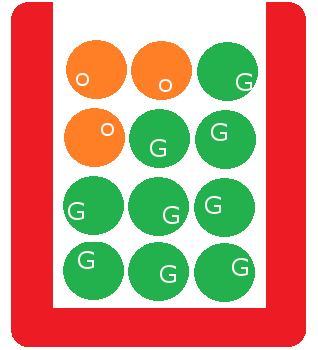
\includegraphics[width=2in]{02Background/prob/RedUrnMarked.png}
	\end{center}
	\caption[ตัวอย่างความน่าจะเป็น ลังใส่ลูกบอล]{ลังใส่ลูกบอล ซึ่งมีลูกบอลอยู่ภายใน $12$ ลูก เป็นลูกบอลสีส้มสามลูก และที่เหลือเป็นสีเขียว}
	\label{fig: prob red box}
\end{figure}
%

%
\begin{figure}
	\begin{center}
		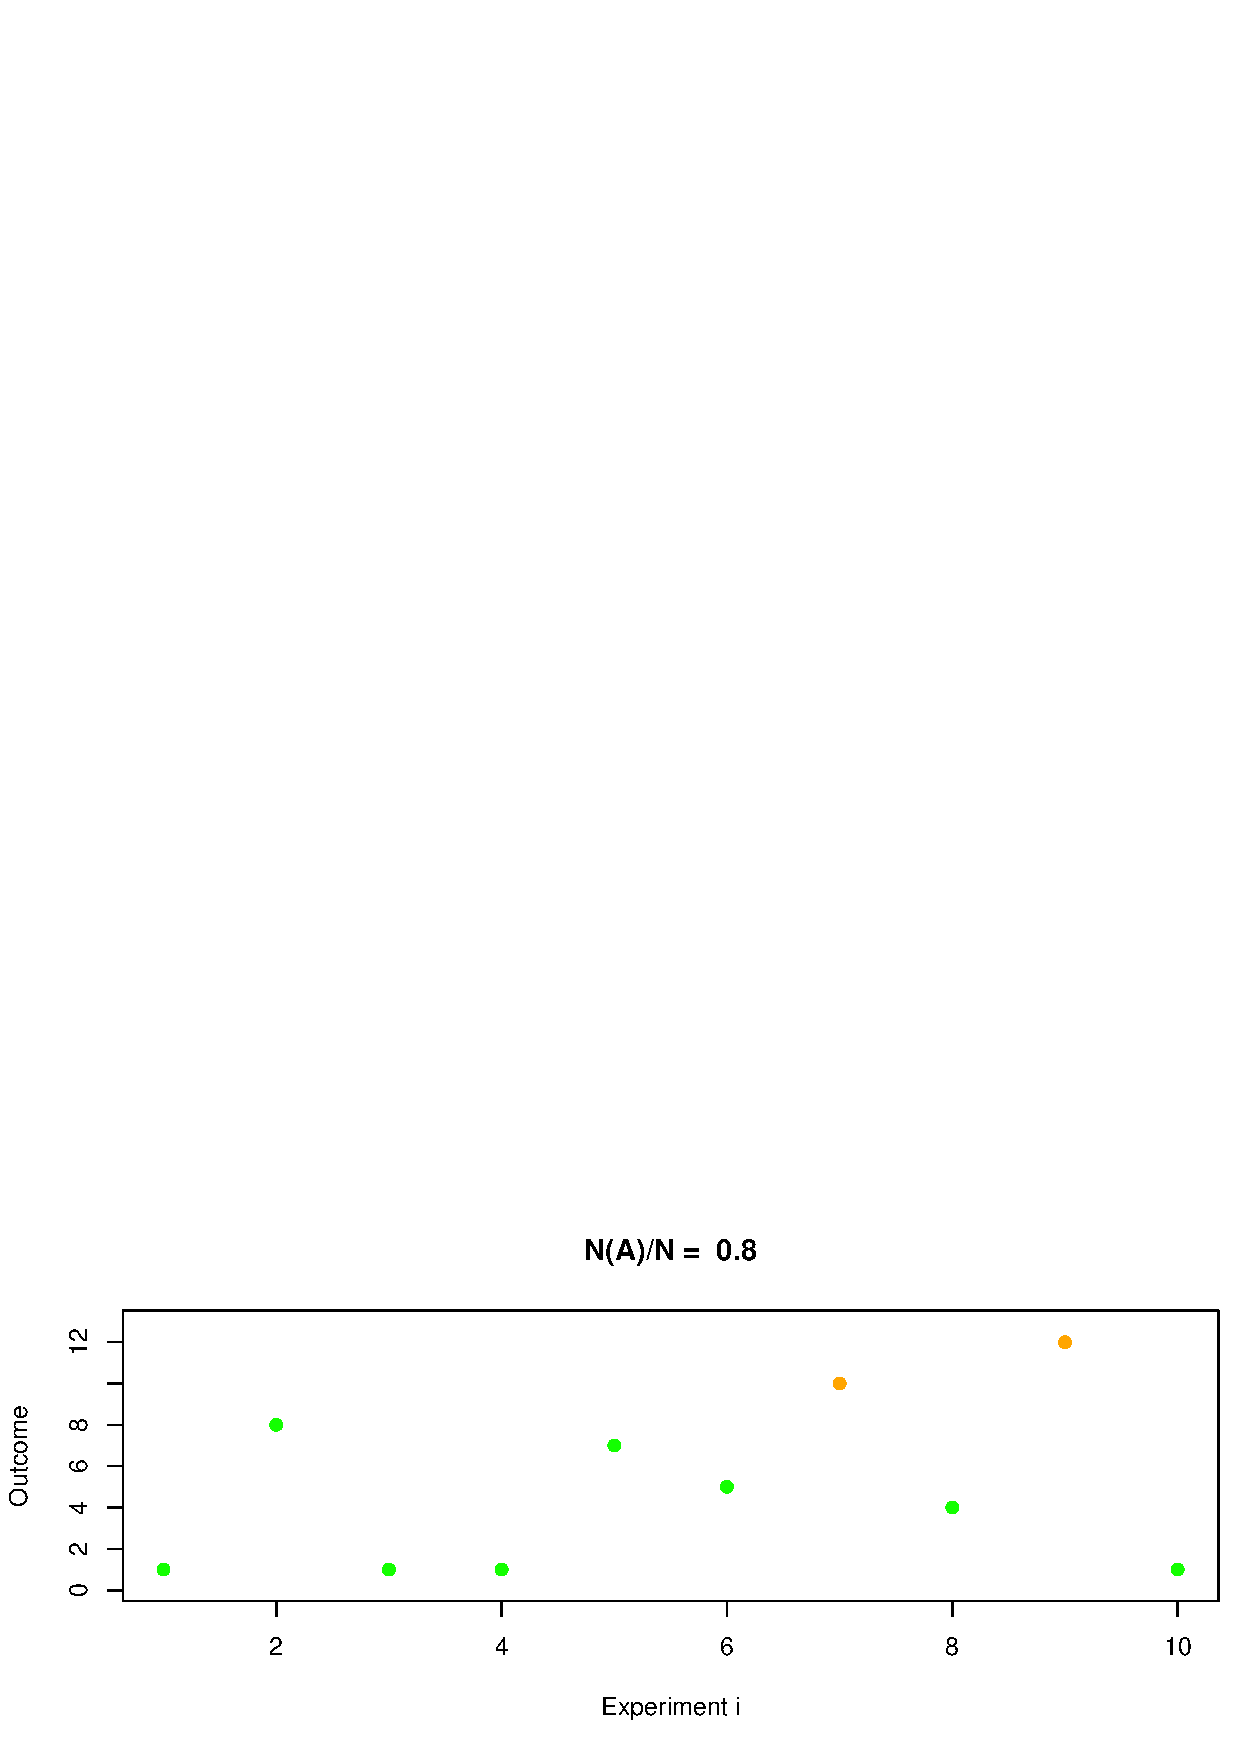
\includegraphics[width=4in]{02Background/prob/probDemo01.png}
	\end{center}
	\caption[ผลจากจำลองสุ่มหยิบลูกบอล]{ผลจากจำลองเหตุการณ์สุ่มหยิบลูกบอล $10$ ครั้ง จากกล่องลูกบอลที่แสดงในรูป~\ref{fig: prob red box}.
		%  ในกล่องมีลูกบอล $12$ ลูก,
		ลูกที่ 1--9 สีเขียว ลูกที่ 10--12 สีส้ม.
		จากการสุ่มทำ $10$ ครั้ง มีครั้งที่ 7 และ 9 ที่หยิบได้ลูกบอลสีส้ม.
		ดังนั้น อัตราส่วนจำนวนครั้งที่หยิบได้ลูกบอลสีเขียว คือ $0.8$ (ระบุที่ด้านบนของภาพ)}
	\label{fig: prob red box result N 10}
\end{figure}
%

\begin{table}[hbtp]
%	{\scriptsize
		\caption[อัตราส่วนของการหยิบได้สีเขียว]{อัตราส่วนของการสุ่มได้ลูกบอลสีเขียว เมื่อจำนวนการทำซ้ำเพิ่มขึ้น}
		\begin{center}
			\begin{tabular}{|r|c|c|c|c|c|c|c|}
				\hline 
				$N$ & $10$ & $100$ & $1000$ & $10^4$ & $10^5$ & $10^6$ & $10^7$ \\
				\hline 
				$\frac{N(A)}{N}$ &
				$0.8$  & $0.68$  & $0.754$  & $0.7564$ & $0.74917$ & $0.749291$ &  $0.7499472$ \\
				\hline
			\end{tabular} 
		\end{center}
		\label{tbl: prob demo N(A)/N}
%	}%end \small
\end{table}

%
\begin{figure}
	\begin{center}
		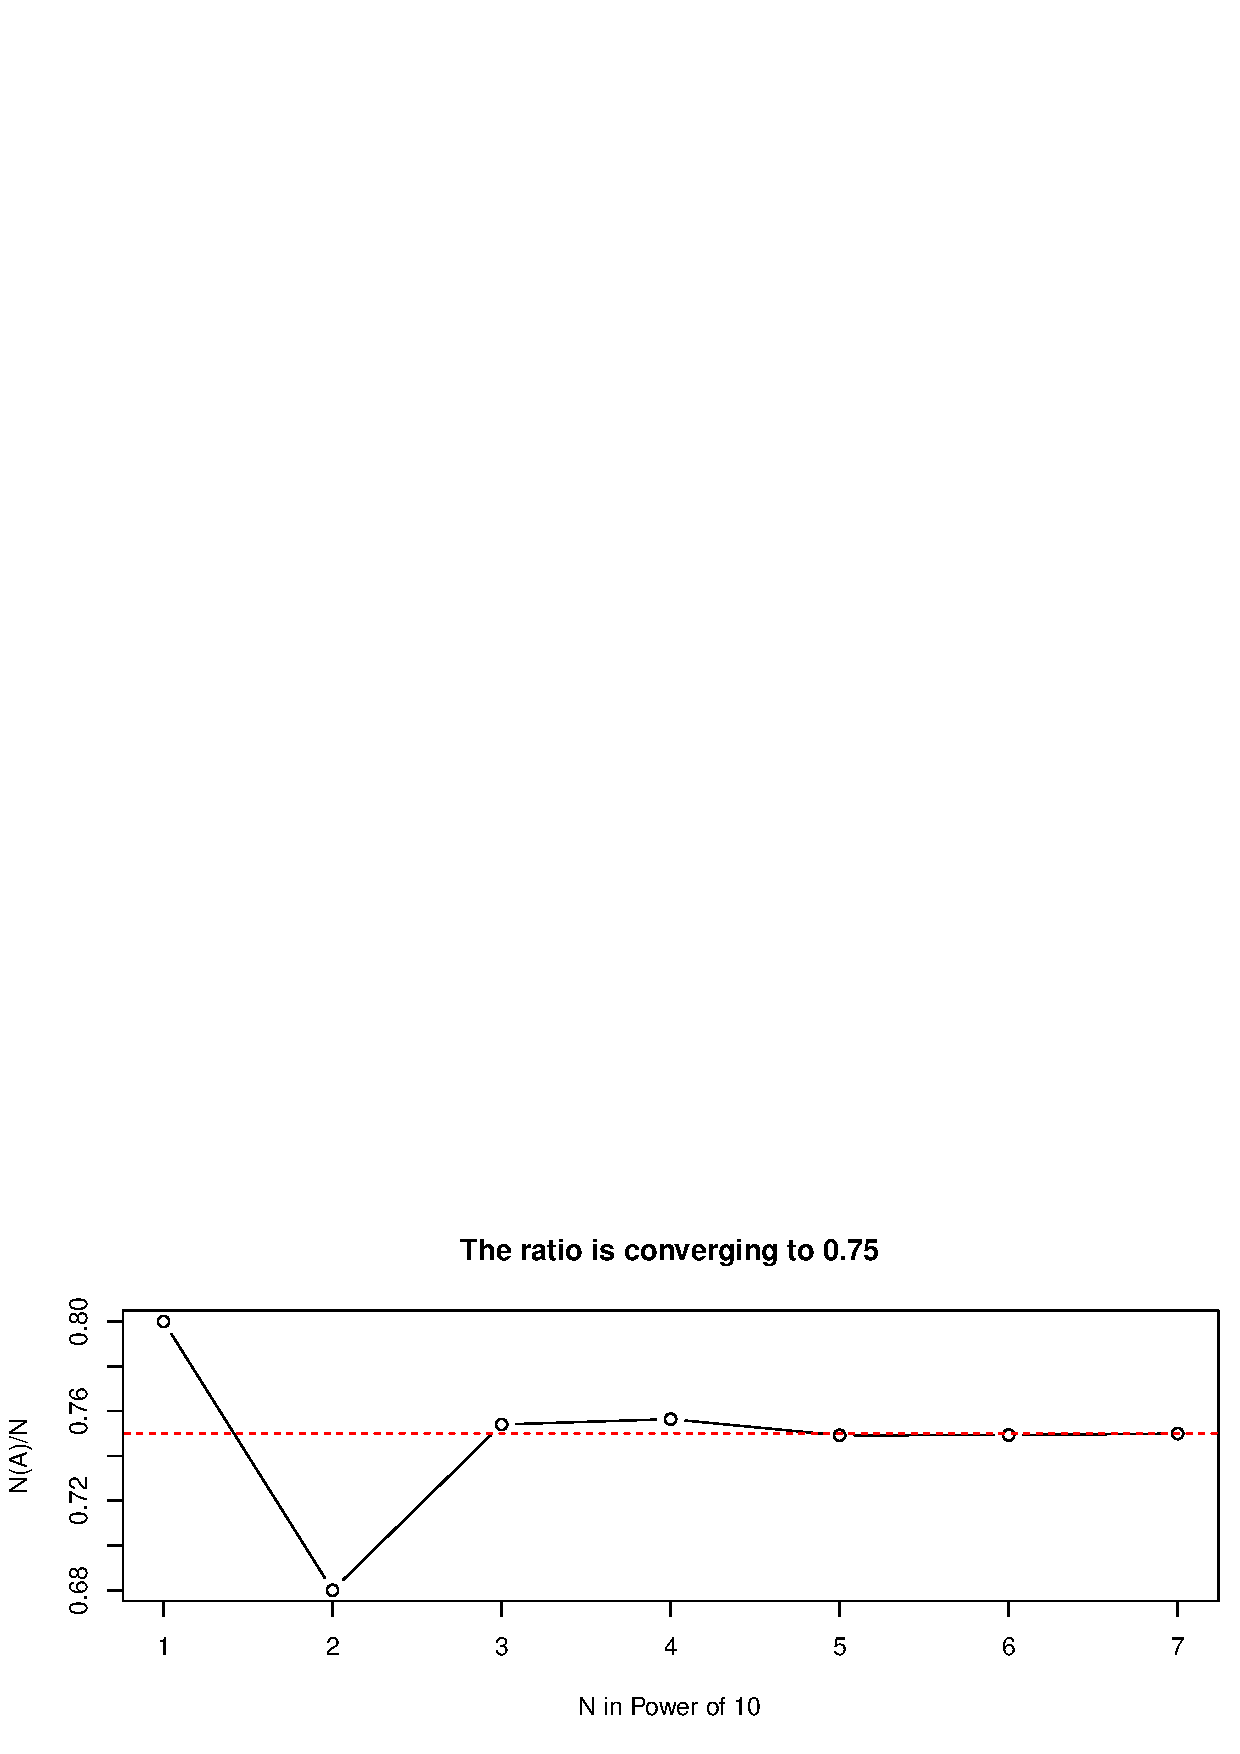
\includegraphics[width=4in]{02Background/prob/demoProb02.png}
	\end{center}
	\caption[การลู่เข้าของอัตราส่วนการหยิบได้สีเขียว]{อัตราส่วน $\frac{N(A)}{N}$ ลู่เข้าหา $\mathrm{Pr}(A) = 0.75$ เมื่อ $N$ เพิ่มขึ้น (แสดงด้วยเส้นประสีแดง)}
	\label{fig: prob demo N(A)/N}
\end{figure}
%

%
\begin{figure}
	\begin{center}
		
		\begin{tabular}{cc}
			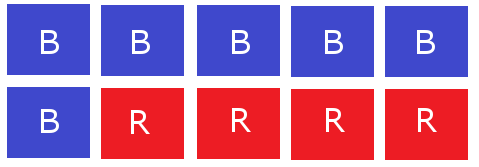
\includegraphics[width=2in]{02Background/prob/boxesMarked.png}
			&
			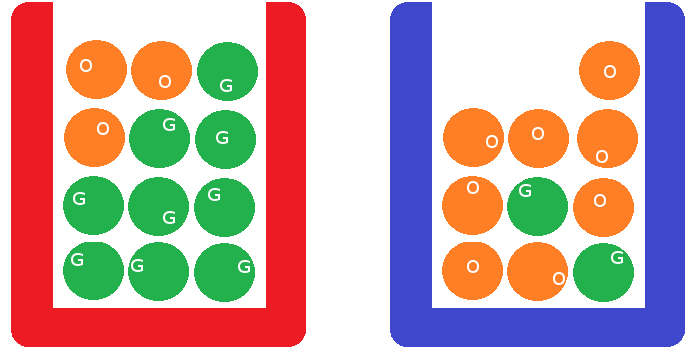
\includegraphics[width=2in]{02Background/prob/TwoUrnsMarked.png}
			\\
			(a) & (b) \\
		\end{tabular} 
	\end{center}
	\caption[ตัวอย่างความน่าจะเป็นแบบมีเงื่อนไข]{ตัวอย่างลังบรรจุลูกบอลสี.
		ภาพ (a) แสดงจำนวนลังสีฟ้ากับลังสีแดง (มีลังสีแดงอยู่ $4$ ลัง ที่เหลือเป็นสีฟ้า).
		ภาพ (b) แสดงลูกบอลสีภายในลัง โดย
		ลังซ้ายสีแดงมีลูกบอลสีส้มอยู่ $3$ ลูก ที่เหลือสีเขียว
		และลังขวาสีฟ้ามีลูกบอลสีเขียวอยู่ $2$ ลูก ที่เหลือสีส้ม}
	\label{fig: prob boxes}
\end{figure}
%

\paragraph{คุณสมบัติของความน่าจะเป็น.}
ความน่าจะเป็นมีคุณสมบัติที่น่าสนใจหลายอย่าง
เช่น
ความน่าจะเป็นที่จะเกิดผลลัพธ์จากกลุ่มผลลัพธ์ทั้งหมดทุกแบบที่เป็นไปได้ คือ ต้องพบแน่นอน ความน่าจะเป็นมีค่าสูงสุด.
นั่นคือ
$\mathrm{Pr}(\Omega) = 1$.
ความน่าจะเป็นที่จะพบเหตุการณ์ที่เป็นไปไม่ได้ คือ ต้องไม่พบแน่นอน ความน่าจะเป็นมีค่าต่ำสุด.
นั่นคือ
$\mathrm{Pr}(\emptyset) = 0$.
ความสัมพันธ์ระหว่างความน่าจะเป็นของเหตุการณ์ $A$ 
กับส่วนเติมเต็ม $A^c$ คือ
$\mathrm{Pr}(A) = 1 - \mathrm{Pr}(A^c)$
และ $\mathrm{Pr}(A \cup A^c) = 1$ 
และ $\mathrm{Pr}(A \cap A^c) = 0$.
ความน่าจะเป็นของยูเนียน คือ
$\mathrm{Pr}(A \cup B) = \mathrm{Pr}(A \setminus B) + \mathrm{Pr}(B \setminus A) + \mathrm{Pr}(A \cap B)$
หรือ
$\mathrm{Pr}(A \cup B) = \mathrm{Pr}(A) + \mathrm{Pr}(B) - \mathrm{Pr}(A \cap B)$.
ความน่าจะเป็นของผลต่าง คือ
$\mathrm{Pr}(A \setminus B) = \mathrm{Pr}(A) - \mathrm{Pr}(A \cap B)$.

\paragraph{เหตุการณ์ที่ไม่มีส่วนร่วมกัน.}
ถ้า $A \cap B = \emptyset$ 
แล้วจะเรียกว่า เหตุการณ์ $A$ และเหตุการณ์ $B$ \textbf{ไม่มีส่วนร่วมกัน} (disjoint)
\index{english}{probability!disjoint}
\index{thai}{ความน่าจะเป็น!ไม่มีส่วนร่วมกัน}
และยูเนียนของเหตุการณ์ที่ไม่มีส่วนร่วมกัน จะมีความน่าจะเป็น $\mathrm{Pr}(A \cup B) = \mathrm{Pr}(A) + \mathrm{Pr}(B)$.

\paragraph{กฎของการรวมความน่าจะเป็น.}
ถ้า $B_1 \cup B_2 \cup \cdots \cup B_n = \Omega$
และ $B_i \cap B_j = \emptyset$ สำหรับทุกๆค่าของ $i \neq j$ ตั้งแต่ $1, \ldots, n$
แล้ว
\textbf{กฎของความน่าจะเป็นรวม} (law of total probability)
\index{english}{probability!sum rule}
\index{english}{law of total probability}
\index{thai}{กฎของความน่าจะเป็นรวม}
กล่าวว่า
\begin{eqnarray}
\mathrm{Pr}(A) = \sum_{i=1}^n \mathrm{Pr}(A \cap B_i)
\label{eq: prob law of total prob}
\end{eqnarray}
จาก\textit{กฎของความน่าจะเป็นรวม}
กรณีพิเศษ คือ $\mathrm{Pr}(A) = \mathrm{Pr}(A \cap B) + \mathrm{Pr}(A \cap B^c)$.

\paragraph{ตัวแปรสุ่ม.}
\index{thai}{ตัวแปรสุ่ม}
\index{english}{random variable}
เพื่อความสะดวก
เหตุการณ์อาจถูกระบุด้วย
\textit{ตัวแปรสุ่ม} 
เช่น จากตัวอย่าง
เหตุการณ์ที่หยิบได้ลูกบอลสีเขียว
และเหตุการณ์ที่หยิบได้ลูกบอลสีส้ม
จะสามารถถูกอ้างถึงได้สะดวก และชัดเจนกว่า
ถ้ากำหนด \textit{ตัวแปรสุ่ม} $B$ แทนสีของลูกบอลที่ถูกสุ่มหยิบขึ้นมา.
เหตุการณ์ที่หยิบได้ลูกบอลสีเขียว 
สามารถ เขียนเป็น $B = 0$
เมื่อ $0$ แทนสีเขียว %\mbox{`g'}$
และ 
เหตุการณ์ที่หยิบได้ลูกบอลสีส้ม 
สามารถ เขียนเป็น $B = 1$
เมื่อ $1$ แทนสีส้ม.
\textbf{ตัวแปรสุ่ม} (random variable)
อาจถูกนิยามว่า
เป็นตัวแปรที่ค่าของมันขึ้นกับผลลัพธ์ของเรื่องที่สนใจ เมื่อเรื่องที่สนใจเป็นกระบวนการที่มี\textit{ความไม่แน่นอน}อยู่.
%a variable whose values depend on outcomes of a random phenomenon

หมายเหตุ \textit{ตัวแปรสุ่ม}เป็นการแทน\textit{เหตุการณ์}ด้วยค่าตัวเลข
โดยสำหรับธรรมชาติของเหตุการณ์ที่ไม่ได้เป็นตัวเลข การใช้งานตัวแปรสุ่มนี้อาจทำได้โดยการกำหนดความหมายให้กับตัวเลข 
เช่น $0$ แทนสีเขียว และ $1$ แทนสีส้ม.
แต่หลาย ๆ ครั้งเพื่อความสะดวกและชัดเจน
อาจมีการใช้สัญลักษณ์ เช่น
$\mbox{`g'}$ แทนตัวเลข $0$ ในกรณีที่ระบุถึงสีเขียว.

\textbf{ฟังก์ชันการแจกแจง} (distribution function)
	\index{thai}{ฟังก์ชันการแจกแจง}
	\index{english}{distribution function}
	ของ\textit{ตัวแปรสุ่ม} $X$
คือฟังก์ชัน 
$F: \mathbb{R} \rightarrow [0,1]$ 
โดย
\begin{eqnarray}
F(x) = \mathrm{Pr}(X \leq x)
\label{eq: cdf}
\end{eqnarray}
เมื่อ $x$ เป็นค่าของตัวแปรสุ่ม $X$.

สังเกตว่า เนื่องจาก\textit{ฟังก์ชันการแจกแจง} สื่อถึงค่าความน่าจะเป็นของเหตุการณ์ต่าง ๆ
ที่ตัวแปรสุ่มมีค่าจนถึงค่า $x$ ที่กำหนด
ดังนั้น%
\textit{ฟังก์ชันการแจกแจง}นี้
บางครั้งอาจเรียก
\textbf{ฟังก์ชันการแจกแจงสะสม} (cumulative distribution function คำย่อ cdf).
\index{english}{cumulative distribution function}
\index{thai}{ฟังก์ชันการแจกแจงสะสม}

ตัวแปรสุ่มอาจมีได้หลายแบบขึ้นกับลักษณะของค่าของมัน ซึ่งค่าของมันก็คือลักษณะของผลลัพธ์ที่เป็นไปได้.
\textbf{ตัวแปรสุ่มวิยุต} (discrete random variable)
คือตัวแปรสุ่มที่ค่าของมัน อยู่ใน\textit{เซตจำกัด} (finite set) หรืออยู่ใน\textit{เซตไม่จำกัดแต่นับได้} (countably infinite set).
ตัวอย่าง \textit{ตัวแปรสุ่ม}สีของลูกบอล $B$ นี้เป็น\textit{ตัวแปรสุ่มวิยุต}
เนื่องจากค่าของมันมาจาก\textit{เซตจำกัด} ได้แก่ $\{0, 1\}$ (มีจำนวนสมาชิกน้อยกว่าค่าอนันต์ $\infty$).
\textit{ตัวแปรสุ่ม}จำนวนต้นทุเรียน ก็เป็น\textit{ตัวแปรสุ่มวิยุต}
เนื่องจากค่าของมันมาจาก\textit{เซตไม่จำกัดแต่นับได้} ได้แก่ $\{0, 1, 2, 3, \ldots \}$.
แต่\textit{ตัวแปรสุ่ม}ปริมาณน้ำในอ่างเก็บน้ำ ไม่ใช่\textit{ตัวแปรสุ่มวิยุต}
เพราะว่า ค่าของมันมาจาก $\mathbb{R}^+$ 
%เช่น ปริมาณน้ำปีนี้อาจจะน้อยเหลือแค่ $8203046.91$ ลบ.ม.
\textit{ตัวแปรสุ่ม}ปริมาณน้ำในอ่างเก็บน้ำ จะเป็น\textit{ตัวแปรสุ่มต่อเนื่อง}.
หัวข้อ~\ref{sec: continuous random variable} อภิปราย\textit{ตัวแปรสุ่มต่อเนื่อง}เพิ่มเติม.

\textit{ตัวแปรสุ่มวิยุต} $X$ จะมี\textbf{ฟังก์ชันมวลความน่าจะเป็น} (probability mass function คำย่อ pmf) $f: \mathbb{R} \rightarrow [0,1]$ โดย $f(x) = \mathrm{Pr}(X = x)$.
\index{english}{probability mass function}
\index{english}{probability!mass function}
\index{english}{pmf}
\index{thai}{ฟังก์ชันมวลความน่าจะเป็น}


%\paragraph{ค่าคาดหมาย.}
\textbf{ค่าคาดหมาย} (expectation หรือ expected value) 
\index{english}{expectation}
\index{english}{expected value}
\index{thai}{ค่าคาดหมาย}
เป็น\textit{ค่าเฉลี่ย}ของ\textit{ตัวแปรสุ่ม}
และใช้สัญกรณ์ เช่น $E[X]$
สำหรับค่าคาดหมายของตัวแปรสุ่ม $X$.
โดยสำหรับ\textit{ตัวแปรสุ่มวิยุต}ที่เป็นตัวเลข
\textit{ค่าคาดหมาย}สามารถคำนวณได้จาก
\begin{eqnarray}
E[X] &=& \sum_x x \cdot \mathrm{Pr}(X=x)
\label{eq: prob expectation}.
\end{eqnarray}


\textbf{ความแปรปรวน} (variance)
\index{thai}{ความแปรปรวน}
\index{english}{variance}
ของ\textit{ตัวแปรสุ่ม}
ใช้สัญกรณ์ เช่น
$\mathrm{var}[X]$
ซึ่งค่า\textit{ความแปรปรวน} คำนวณได้จาก
\begin{eqnarray}
\mathrm{var}[X] &=& 
E[(X -E[X])^2]
\label{eq: prob variance}
\end{eqnarray}

% LATER
% ตัวอย่าง

\paragraph{ความน่าจะเป็นร่วม.}
\index{thai}{ความน่าจะเป็นร่วม}
\index{english}{joint probability}
\index{english}{probability!joint}
เมื่อใช้\textit{ตัวแปรสุ่ม}อธิบายเหตุการณ์
ในกรณีที่สนใจเหตุการณ์ที่เกี่ยวข้องกับ\textit{ตัวแปรสุ่ม}ตั้งแต่สองตัวขึ้นไป 
ความน่าจะเป็นที่ใช้ จะเรียกว่า
\textbf{ความน่าจะเป็นร่วม} (joint probability)
และใช้สัญกรณ์ 
เช่น $\mathrm{Pr}(X, Y)$ หรือ\textbf{ความน่าจะเป็นร่วม}ของ\textit{ตัวแปรสุ่ม} $X$ และ\textit{ตัวแปรสุ่ม} $Y$
และ\textit{ความน่าจะเป็นร่วม}
$\mathrm{Pr}(X, Y) = \mathrm{Pr}(X \cap Y)$.
นั่นคือ
$\mathrm{Pr}(X = x, Y = y)$
หมายถึง
ความน่าจะเป็นที่
\textit{ตัวแปรสุ่ม} $X$ จะมีค่าเป็น $x$
และ\textit{ตัวแปรสุ่ม} $Y$ จะมีค่าเป็น $y$.
%(หมายเหตุ สัญกรณ์ เช่น $\mathrm{Pr}(X, Y)$ เป็นการระบุถึง\textit{ความน่าจะเป็นร่วม}
%ในลักษณะทั่วไป และมักจะใช้เมื่อพิจารณรูปสมการที่แสดงความสัมพันธ์ระหว่างค่าตัวแปรสุ่มและค่าความน่าจะเป็น.)
%= placeholder

\textbf{ความแปรปรวนร่วมเกี่ยว} (covariance)
\index{thai}{ความแปรปรวนร่วมเกี่ยว}
\index{english}{covariance}
ของ\textit{ตัวแปรสุ่ม}สองตัว
ใช้สัญกรณ์ เช่น
$\mathrm{cov}[X, Y]$
ซึ่งค่า\textit{ความแปรปรวนร่วมเกี่ยว} คำนวณได้จาก
\begin{eqnarray}
\mathrm{cov}[X, Y] &=& 
E_{X,Y}[(X - E[X])(Y - E[Y])]
\nonumber \\
&=& E_{X,Y}[XY] - E[X]E[Y]
\label{eq: prob covariance}
\end{eqnarray}
เมื่อ $E_{X,Y}$ หมายถึง\textit{ค่าคาดหมาย} ที่คิดโดยคำนึงถึงความน่าจะเป็นร่วมของ $X$ และ $Y$.
นั่นคือ
สำหรับตัวแปรสุ่มวิยุต
$ 
\mathrm{cov}[X, Y] =
\sum_x \sum_y (x - E[X])(y - E[Y]) \cdot \mathrm{Pr}(X=x, Y=y)$.


\subsection{ความน่าจะเป็นแบบมีเงื่อนไข} 
\label{sec: cond prob}
\index{english}{conditional probability}
\index{thai}{ความน่าจะเป็นแบบมีเงื่อนไข}
\index{english}{probability!conditional}
\index{thai}{ความน่าจะเป็น!แบบมีเงื่อนไข}

\textbf{ความน่าจะเป็นแบบมีเงื่อนไข} (conditional probability) 
ประมาณโอกาสที่จะเกิดเหตุการณ์ที่สนใจ ในกรณีที่รู้ผลลัพธ์ของเงื่อนไข.
\textit{ความน่าจะเป็นแบบมีเงื่อนไข}จะเน้นบริบทของเงื่อนไข.
สัญกรณ์ เช่น $\mathrm{Pr}(A|B)$ 
แทน\textit{ความน่าจะเป็นแบบมีเงื่อนไข} 
ที่หมายถึง \textit{ความน่าจะเป็น}ของเหตุการณ์ $A$
ในกรณีที่เหตุการณ์ $B$ เป็นจริง.
เหตุการณ์ $B$ เป็นเงื่อนไข
และเป็นบริบทเสริม เป็นข้อมูลเสริมในการประมาณความน่าจะเป็น.

จากตัวอย่างของรูป~\ref{fig: prob red box} 
พิจารณาตัวอย่างที่คราวนี้
มีลังอยู่ $10$ ลัง ซึ่ง เป็นลังสีแดง $4$ ลัง และเป็นลังสีบานเย็น $6$ ลัง ดังรูป~\ref{fig: prob boxes}.
ถ้าสุ่มยกมาหนึ่งลัง โอกาสที่จะเป็นลังที่ 7 คือ $1/10$
แต่ถ้าเห็นว่าลังที่สุ่มมาเป็นสีแดง โอกาสที่จะเป็นลังที่ 7 คือ $1/4$ เพราะว่า มีแค่ลังที่ 7 ถึงลังที่ 10 ที่เป็นสีแดงอยู่แค่ $4$ ลัง.
ถ้าเห็นว่าลังที่สุ่มมาสีบานเย็น โอกาสที่จะเป็นลังที่ 7 ไม่มีเลย หรือโอกาสเป็น $0$ เพราะลังที่ 7 สีแดง.
ข้อมูลพิเศษ หรือบริบทเพิ่มเติมนี้ คือเงื่อนไขที่ใช้ประกอบการประมาณโอกาสของเหตุการณ์.


\paragraph{การคำนวณ.}
ความน่าจะเป็นแบบมีเงื่อนไข
สามารถคำนวณได้จาก
\begin{eqnarray}
\mathrm{Pr}(A|B) = \frac{\mathrm{Pr}(A \cap B)}{\mathrm{Pr}(B)}
\label{eq: prob cond prob relation}
\end{eqnarray}
เมื่อ $\mathrm{Pr}(B) > 0$.
จากสมการ~\ref{eq: prob cond prob relation} จะได้
\begin{eqnarray}
\mathrm{Pr}(X, Y) = \mathrm{Pr}(X|Y) \cdot \mathrm{Pr}(Y)
\label{eq: prob product rule}
\end{eqnarray}
เมื่อ $X$ และ $Y$ คือตัวแปรสุ่ม.
สมการ~\ref{eq: prob product rule} มักเรียกว่า \textbf{กฎผลคูณ} (product rule).
\index{english}{product rule}
\index{thai}{กฎผลคูณ}
นอกจากนั้น พิจารณาสมการ~\ref{eq: prob law of total prob} และ~\ref{eq: prob product rule}  จะพบว่า 
\begin{eqnarray}
\mathrm{Pr}(X) = \sum_y \mathrm{Pr}(X, Y=y) = \sum_y \mathrm{Pr}(X|Y = y) \cdot \mathrm{Pr}(Y = y) 
\label{eq: prob sum rule}
\end{eqnarray}
ซึ่ง สมการนี้มักเรียกว่า \textbf{กฎผลรวม} (sum rule).
\index{english}{sum rule}
\index{thai}{กฎผลรวม}
สังเกตว่า การใช้\textit{กฎผลรวม}
จะลดตัวแปรสุ่มลงไป
ซึ่งการทำเช่นนี้ 
จึงอาจถูกเรียกว่า \textit{การสลายปัจจัย} (marginalization).
\index{english}{marginalization}
\index{thai}{การสลายปัจจัย}



\textit{กฎผลคูณ}สามารถใช้ต่อเนื่องกัน ในลักษณะลูกโซ่
\begin{eqnarray}
\mathrm{Pr}(X_1, X_2, \ldots, X_n) 
&=& \mathrm{Pr}(X_1) \cdot \mathrm{Pr}(X_2, \ldots, X_n|X_1)
\nonumber \\
&=& \mathrm{Pr}(X_1) \cdot \mathrm{Pr}(X_2|X_1)
\cdot \mathrm{Pr}(X_3, \ldots, X_n|X_1, X_2)
\nonumber \\
&\vdots& 
\nonumber \\
&=& \mathrm{Pr}(X_1) \cdot \mathrm{Pr}(X_2|X_1)
\cdot \mathrm{Pr}(X_3|X_1, X_2)
\cdot \mathrm{Pr}(X_4|X_1, X_2, X_3)
\cdot \cdots
\nonumber \\
&\;& \;
\cdots \mathrm{Pr}(X_n|X_1, \ldots, X_{n-1})
\label{eq: prob chain rule}
\end{eqnarray}
ซึ่งสมการ~\ref{eq: prob chain rule} มักจะถูกเรียกว่า \textbf{กฎลูกโซ่ของความน่าจะเป็น} (chain rule of probability).
\index{thai}{กฎลูกโซ่ของความน่าจะเป็น}
\index{english}{chain rule of probability}

\textbf{กฎของเบส์} (Bayes' rule หรือ Bayes' theorem)
\index{thai}{กฎของเบส์}
\index{english}{Bayes' rule}
\index{english}{Bayes' theorem} 
คือ
\begin{eqnarray}
\mathrm{Pr}(Y|X) &=& \frac{\mathrm{Pr}(X|Y) \cdot \mathrm{Pr}(Y)}{\mathrm{Pr}(X)}
\label{eq: prob Bayes' 1} \\
&=&
\frac{\mathrm{Pr}(X|Y) \cdot \mathrm{Pr}(Y)}{\sum_y \mathrm{Pr}(X|Y=y) \cdot \mathrm{Pr}(Y=y)}
\label{eq: prob Bayes' 2}
\end{eqnarray}
จากความสัมพันธ์ที่ได้จาก\textit{กฎของเบส์}
การอนุมานค่าที่สนใจจากข้อมูล
มักจะเรียกชื่อพจน์ต่าง ๆ
ในสมการ~\ref{eq: prob Bayes' 1} เพื่อความสะดวก ดังนี้
ถ้ากำหนดให้ตัวแปรสุ่ม $Y$ แทนเป้าหมายของการอนุมาน
และตัวแปรสุ่ม $X$ แทนข้อมูลประกอบ
แล้ว
$\mathrm{Pr}(Y)$ จะเรียกว่า \textit{ความน่าจะเป็นก่อน}
(prior probability คำย่อ prior)
ซึ่งหมายถึง ก่อนการนำข้อมูลประกอบมาคิด
$\mathrm{Pr}(Y|X)$ จะเรียกว่า
\textit{ความน่าจะเป็นภายหลัง}
(posterior probability คำย่อ posterior)
ซึ่งหมายถึง ภายหลังการนำข้อมูลประกอบมาคิด
และ
หาก $\mathrm{Pr}(X|Y)$ เขียนอยู่ในรูปฟังก์ชัน $f(y) = \mathrm{Pr}(X|Y=y)$
ก็จะถูกเรียกว่า \textit{ฟังก์ชันควรจะเป็น} (likelihood function คำย่อ likelihood).
ดังนั้น จาก\textit{กฎของเบส์}
และชื่อพจน์ต่าง ๆ อาจสรุปความสัมพันธ์ได้เป็น
$\mathrm{posterior} \propto \mathrm{likelihood} \cdot \mathrm{prior}$.

\paragraph{ตัวอย่างการคำนวณ.}
กลับมาที่รูป~\ref{fig: prob boxes}
อีกครั้ง คราวนี้จะสุ่มเลือกลัง และพอได้ลังแล้วก็จะสุ่มหยิบลูกบอลออกมา.
โอกาสที่จะสุ่มได้ลังแดงเป็น $\frac{4}{10}$ หรือความน่าจะเป็นที่จะได้ลังสีแดง $\mathrm{Pr}(C = \mbox{`r'}) = 0.4$
โดย $C = \mbox{`r'}$ แทนเหตุการณ์ที่จะได้ลังสีแดง.
ในทำนองเดียวกัน ความน่าจะเป็นที่จะได้ลังสีบานเย็น $\mathrm{Pr}(C = \mbox{`m'}) = 0.6$.

ถ้ารู้ว่าเป็นลังสีแดง เมื่อสุ่มหยิบลูกบอลมา โอกาสที่จะหยิบได้ลูกบอลสีเขียว คือ $\frac{9}{12} = 0.75$ 
หรือเขียนเป็นสัญกรณ์ ได้ว่า
$\mathrm{Pr}(B = \mbox{`g'}|C = \mbox{`r'}) = 0.75$
โดย $B = \mbox{`g'}$ แทนเหตุการณ์ที่จะหยิบได้ลูกบอลสีเขียว.
ทำนองเดียวกัน ก็จะได้\textit{ความน่าจะเป็นแบบมีเงื่อนไข}อื่น ๆ ดังนี้
\begin{itemize}
	\item $\mathrm{Pr}(B = \mbox{`o'}|C = \mbox{`r'}) = 0.25$,
	\item $\mathrm{Pr}(B = \mbox{`g'}|C = \mbox{`m'}) = 0.20$, 
	\item $\mathrm{Pr}(B = \mbox{`o'}|C = \mbox{`m'}) = 0.80$.
	\hfill $\#$%$\square$	
\end{itemize}

สังเกตว่า \textit{ความน่าจะเป็นที่จะหยิบได้ลูกบอลสีเขียวเมื่อรู้ว่าลังสีแดง} $\mathrm{Pr}(B = \mbox{`g'}|C = \mbox{`r'})$ ไม่เหมือนกับ\textit{ความน่าจะเป็นที่จะหยิบลูกบอลสีเขียวและสุ่มได้ลังสีแดง} $\mathrm{Pr}(B = \mbox{`g'}, C = \mbox{`r'})$.
สำหรับ
$\mathrm{Pr}(B = \mbox{`g'}|C = \mbox{`r'}) = 0.75$
นั้นไม่ต้องสนใจเลยว่าโอกาสที่จะได้ลังสีแดงเป็นเท่าไร.
ในขณะที่
$\mathrm{Pr}(B = \mbox{`g'}, C = \mbox{`r'})$ จะประกอบด้วยโอกาสที่จะได้ลังสีแดง $\mathrm{Pr}(C = \mbox{`r'}) = 0.4$ และโอกาสที่จะหยิบได้ลูกบอลสีเขียวจากลังนั้น $\mathrm{Pr}(B = \mbox{`g'}|C = \mbox{`r'}) = 0.75$
ซึ่งจาก\textit{กฎผลคูณ} (สมการ~\ref{eq: prob product rule})
จะได้
\begin{eqnarray}
\mathrm{Pr}(B = \mbox{`g'}, C = \mbox{`r'}) &=& \mathrm{Pr}(C = \mbox{`r'}) \cdot \mathrm{Pr}(B = \mbox{`g'}|C = \mbox{`r'})
\nonumber \\
&=& (0.4) \cdot (0.75) = 0.3
\nonumber .
\end{eqnarray}

ในทำนองเดียวกันก็จะได้ค่าความน่าจะเป็นต่าง ๆ
ดังแสดงในตาราง~\ref{tbl: prob cond prob table}.

ทบทวน (1) ผลรวมของความน่าจะเป็นของทุก ๆ เหตุการณ์เป็น $1$. 
นั่นคือ
\begin{eqnarray}
\mathrm{Pr}(\Omega) &=& \mathrm{Pr}(C = \mbox{`r'}, B = \mbox{`g'})
+ \mathrm{Pr}(C = \mbox{`r'}, B = \mbox{`o'})
\nonumber \\
&\;&  
+ \mathrm{Pr}(C = \mbox{`b'}, B = \mbox{`g'})
+ \mathbb{P}(C = \mbox{`b'}, B = \mbox{`o'})    
\nonumber \\
&=& 0.3 + 0.1 + 0.12 + 0.48 = 1
\nonumber .
\end{eqnarray}
ธรรมชาตินี้เป็นคุณสมบัติพื้นฐานของความน่าจะเป็น.
ทบทวน (2) ความน่าจะเป็นของเหตุการณ์ $X$ เท่ากับผลรวมของความน่าจะเป็นของเหตุการณ์ $X$ และ $Y$ สำหรับทุก ๆ ความเป็นไปได้ของ $Y$ 
ดังเช่น
\begin{eqnarray}
\mathrm{Pr}(C = \mbox{`r'}) &=& \mathrm{Pr}(C = \mbox{`r'}, B = \mbox{`g'}) + \mathrm{Pr}(C = \mbox{`r'}, B = \mbox{`o'})
\nonumber \\
&=& 0.3 + 0.1 = 0.4
\nonumber \\
\mathrm{Pr}(C = \mbox{`m'}) &=& \mathrm{Pr}(C = \mbox{`m'}, B = \mbox{`g'}) + \mathrm{Pr}(C = \mbox{`m'}, B = \mbox{`o'})
\nonumber \\
&=& 0.12 + 0.48 = 0.6
\nonumber .
\end{eqnarray}
ธรรมชาตินี้คือ\textit{กฎผลบวก} (สมการ~\ref{eq: prob sum rule}).

จาก\textit{กฎของการบวก}
จะได้ ความน่าจะเป็นที่จะหยิบได้ลูกบอลสีเขียว และสีส้ม (โดยไม่สนใจสีของลัง)
\begin{eqnarray}
\mathrm{Pr}(B = \mbox{`g'}) &=& \mathrm{Pr}(C = \mbox{`r'}, B = \mbox{`g'}) + \mathrm{Pr}(C = \mbox{`m'}, B = \mbox{`g'})
\nonumber \\
&=& 0.3 + 0.12 = 0.42
\nonumber \\
\mathrm{Pr}(B = \mbox{`o'}) &=& \mathrm{Pr}(C = \mbox{`r'}, B = \mbox{`o'}) + \mathrm{Pr}(C = \mbox{`m'}, B = \mbox{`o'})
\nonumber \\
&=& 0.1 + 0.48 = 0.58
\nonumber .
\end{eqnarray}
และความน่าจะเป็นของลังถ้าหากรู้สีของลูกบอลที่สุ่มหยิบออกมาหนึ่งลูก
\begin{eqnarray}
\mathrm{Pr}(C = \mbox{`r'}|B = \mbox{`g'}) &=& \frac{\mathrm{Pr}(B = \mbox{`g'}|C = \mbox{`r'})
	\cdot \mathrm{Pr}(C = `r')}{\mathrm{Pr}(B = \mbox{`g'})}
\nonumber \\
&=& \frac{(0.75) (0.4)}{0.42} = 0.71
\nonumber . 
\end{eqnarray}
\textit{ความน่าจะเป็นแบบมีเงื่อนไข} และ\textit{ทฤษฎีของเบส์}
ช่วยให้สามารถหาค่า\textit{ความน่าจะเป็น}ที่สนใจได้
จาก\textit{ค่าของความน่าจะเป็น}อื่นที่ประเมิน\textit{ความน่าจะเป็น}ได้ง่ายกว่า
เช่น
$\mathrm{Pr}(B|C)$ จะประเมินได้ง่าย 
เพราะว่า ลูกบอลอยู่ในลัง ดังนั้นจะนับได้ง่ายว่า ในลังแต่ละสี มีลูกบอลสีไหนจำนวนเท่าไร ต่อจำนวนลูกบอลทั้งหมดในลัง.
$\mathrm{Pr}(C)$ ก็ประเมินได้ง่าย 
แต่ $\mathrm{Pr}(C|B)$ ประเมินตรง ๆ ได้ยาก
เพราะลูกบอลแต่สีกระจายไปทุก ๆ ลัง.

\begin{table}[hbtp]
	%{\scriptsize
	\caption[สรุปค่าความน่าจะเป็นร่วม]{สรุปค่าความน่าจะเป็นของตัวอย่างการสุ่มลังและลูกบอล}
	\begin{center}
		\begin{tabular}{|c|l|l|}
			\hline 
			ลัง & \multicolumn{2}{c|}{ลูกบอล $B$ } \\
			\cline{2-3}
			$C$ & เขียว `g' & ส้ม `o' \\
			\hline
			แดง `r' & 0.3 & 0.1 \\
			\hline
			บานเย็น `m' & 0.12 & 0.48 \\
			\hline
		\end{tabular} 
	\end{center}
	\label{tbl: prob cond prob table}
	%}%end \small
\end{table}


\paragraph{การตีความและความสับสนที่พบได้บ่อย.}
เพื่อหาความน่าจะเป็นที่จะได้ลูกบอลสีเขียว
$\mathrm{Pr}(B = \mbox{`g'})$
บ่อยครั้งมักถูกคำนวณด้วย
$11/22 = 0.5$ 
ซึ่งได้จากการนับลูกบอลสีเขียว เทียบกับลูกบอลทั้งหมด.
กรณีนี้
ค่าที่ถูกต้อง $\mathrm{Pr}(B = \mbox{`g'}) = 0.42$ 
ไม่เท่ากับ 
$11/22 = 0.5$ 
ซึ่ง $11/22$ ได้จากการนับลูกบอล
โดยเสมือนว่าไม่มีลัง.
กรณีหลังนั้น คือสถานการณ์ที่เทลูกบอลทั้งหมดออกจากลัง และสุ่มหยิบลูกไหนก็ได้.
ในขณะที่ตัวอย่างนี้ ต้องเลือกลังก่อน
ถ้าเลือกลังแล้ว ต้องสุ่มหยิบลูกจากในลังที่เลือก.

สองกรณีนี้ จะเห็นต่างกันชัดเจนมาก 
ถ้าพิจารณากรณี เช่น
ตัวอย่างในรูป~\ref{fig:prob common confusion} 
มีลังสีเหลืองแค่ $1$ ลัง มีลังสีฟ้า $4$ ลัง
แต่ลังสีเหลืองมีลูกบอล $8$ ลูก ที่ทั้งหมดสีเขียว
และลังสีฟ้ามีลูกบอล $2$ ลูก
ที่ทั้งหมดสีส้ม.
เมื่อคิดความน่าจะเป็นแล้วจะพบว่า
กรณีนี้
ถ้าเทลูกบอลทั้งหมดออกจากลัง แล้วสุ่มหยิบโอกาสที่จะได้สีเขียวเป็น $8/16 = 1/2$
แต่ถ้าสุ่มเลือกลังก่อน ลังสีเหลืองมีโอกาสแค่ $1/5$
แล้วโอกาสได้ลูกบอลสีเขียวจากลังนี้เป็น $1$ 
ในขณะที่โอกาสที่จะได้ลังสีฟ้าเป็น $4/5$ แต่โอกาสได้ลูกบอลสีเขียวเป็น $0$
ดังนั้นโอกาสได้ลูกบอลสีเขียวจะเป็นแค่ $(1/5) \cdot 1 + (4/5) \cdot 0 = 1/5$.

%
\begin{figure}
	\begin{center}
		\includegraphics[width=\textwidth]
		{02Background/prob/CommonConfusion.png}
	\end{center}
	\caption[ตัวอย่างเพิ่มเติม ความน่าจะเป็นแบบมีเงื่อนไข]{ตัวอย่างเน้นความต่างระหว่างสุ่มเลือกลังแล้วสุ่มเลือกลูกบอล (ในภาพ) เปรียบเทียบกับเทลูกบอลทั้งหมดมารวมกัน แล้วสุ่มเลือกลูกบอล (ไม่มีภาพ)}
	\label{fig:prob common confusion}
\end{figure}
%

ภาพความเกี่ยวเนื่องของเหตุการณ์ และความน่าจะเป็นร่วม และความน่าจะเป็นแบบมีเงื่อนไข
แสดงในรูป~\ref{fig:prob conditional visualization} สำหรับสองเหตุการณ์
และรูป~\ref{fig:prob conditional 3-event visualization} สำหรับสามเหตุการณ์.

%
\begin{figure}
	\begin{center}
		\includegraphics[width=\textwidth]
		{02Background/prob/cond_set2.png}
	\end{center}
	\caption[ความเกี่ยวเนื่องของสองเหตุการณ์]{ภาพแสดงความเกี่ยวเนื่องของเหตุการณ์ ภาพ ก แสดงเหตุการณ์ $A$ ด้วยวงกลมซ้าย และเหตุการณ์ $B$ ด้วยวงกลมขวา พื้นที่ที่ทับซ้อนกันคือ เหตุการณ์ร่วม $A \cap B$
	พื้นที่ทั้งหมดในกรอบคือผลลัพธ์ทุก ๆ แบบที่เป็นไปได้ ($\Omega$ หรือปริภูมิตัวอย่าง).
	ภาพ ข ความน่าจะเป็น $\mathrm{Pr}(A \cap B)$ มองโอกาสเกิดเหตุการณ์ร่วม $A \cap B$ จากบริบทของทุก ๆ ผลลัพธ์ที่เป็นไปได้. ภาพ ค ความน่าจะเป็น $\mathrm{Pr}(A | B)$ มองโอกาสเกิดเหตุการณ์ร่วม $A \cap B$ จากบริบทของเหตุการณ์ $B$.
    ภาพ ง ความน่าจะเป็น $\mathrm{Pr}(B | A)$ มองโอกาสเกิดเหตุการณ์ร่วม $A \cap B$ จากบริบทของเหตุการณ์ $A$.}
	\label{fig:prob conditional visualization}
\end{figure}
%

%
\begin{figure}
	\begin{center}
		\includegraphics[width=\textwidth]
		{02Background/prob/cond_set3.png}
	\end{center}
	\caption[ความเกี่ยวเนื่องของสามเหตุการณ์]{ภาพแสดงความเกี่ยวเนื่องของเหตุการณ์สามเหตุการณ์ ภาพ ก แสดงเหตุการณ์ $A$ เหตุการณ์ $B$ เหตุการณ์ $C$ ด้วยวงกลม
	พื้นที่ที่ทับซ้อนกันแทนเหตุการณ์ร่วม ฉลาก เช่น \texttt{(A,B)} ระบุเหตุการณ์ร่วม $A \cap B$
	และ \texttt{(A,B,C)} ระบุเหตุการณ์ร่วม $A \cap B \cap C$.
	พื้นที่ทั้งหมดในกรอบคือผลลัพธ์ทุก ๆ  แบบที่เป็นไปได้ ($\Omega$).
	ภาพ ข ความน่าจะเป็น $\mathrm{Pr}(A \cap B \cap C)$ มองโอกาสเกิดเหตุการณ์ร่วม $A \cap B \cap C$ จากบริบทของทุก ๆ ผลลัพธ์ที่เป็นไปได้. ภาพ ค ความน่าจะเป็น $\mathrm{Pr}(A | B, C)$ มองโอกาสเกิดเหตุการณ์ร่วม $A \cap B \cap C$ จากบริบทของเหตุการณ์ร่วม $B \cap C$.
	ภาพ ง ความน่าจะเป็น $\mathrm{Pr}(A, B | C)$ มองโอกาสเกิดเหตุการณ์ร่วม $A \cap B \cap C$ จากบริบทของเหตุการณ์ $C$.}
	\label{fig:prob conditional 3-event visualization}
\end{figure}
%


\paragraph{ความเป็นอิสระต่อกัน.}
เหตุการณ์ $A$ และเหตุการณ์ $B$
จะ\textbf{เป็นอิสระ}ต่อกัน (independent)
ก็ต่อเมื่อ
$\mathrm{Pr}(A \cap B) = \mathrm{Pr}(A) \cdot \mathrm{Pr}(B)$.
ดังนั้น จาก\textit{กฎผลคูณ} $\mathrm{Pr}(A \cap B) = \mathrm{Pr}(A|B) \cdot \mathrm{Pr}(B)$
จะได้ว่า $\mathrm{Pr}(A|B) = \mathrm{Pr}(A)$ เมื่อ $A$ และ $B$ เป็นอิสระต่อกัน.
ความหมายก็คือ
ถ้าเหตุการณ์ $A$ และเหตุการณ์ $B$ เป็นอิสระต่อกันแล้ว การรู้หรือไม่รู้ข้อมูลของ $B$ ก็ไม่ได้เปลี่ยนการประมาณค่าของ $A$.

\subsubsection{ตัวอย่างการใช้งานความน่าจะป็นแบบมีเงื่อนไข}
\label{sec: prob cond prob examples}

\paragraph{ปัญหาการตรวจเต้านมด้วยภาพเอ็กซเรย์.}
สมมติว่า ผู้หญิงอายุสี่สิบปีคนหนึ่ง ไปทำ\textit{การตรวจเต้านมด้วยภาพเอ็กซเรย์} (mammogram)
แล้วผลตรวจเป็น\textit{บวก} (positive ซึ่งหมายถึง เครื่องตรวจบอกว่าเป็นมะเร็ง)
โอกาสที่ผู้หญิงคนนี้จะเป็นมะเร็งจริง ๆ เป็นเท่าไร

สมมติว่าข้อมูลประกอบ คือ
วิธีการตรวจเต้านมด้วยเอ็กซเรย์มี\textit{ค่าความไว} (sensitivity) ที่ $80\%$
ซึ่งหมายความว่า ถ้าคนที่เป็นมะเร็งไปทำการตรวจแล้ว
โอกาสที่จะได้ผลเป็นบวก คือ $0.8$.
นั่นคือ $\mathrm{Pr}(M = 1|C = 1) = 0.8$
เมื่อ $M = 1$ แทนผลตรวจเป็นบวก (ถ้า $M = 0$ คือผลตรวจเป็นลบ)
และ $C = 1$ แทนผู้รับการตรวจเป็นมะเร็งจริง ๆ 
(ถ้า $C = 0$ คือผู้รับการตรวจไม่ได้เป็นมะเร็ง).

ความเข้าใจผิดอย่างหนึ่งที่พบบ่อย
คือ การสรุปว่า ผู้หญิงคนนั้นมีโอกาสเป็นมะเร็ง $80\%$ ซึ่งผิด
เพราะการสรุปนี้ ไม่ได้คำนึงถึง\textit{ความน่าจะเป็นก่อน} นั่นคือ โอกาสที่ผู้หญิงอายุสี่สิบปี
จะเป็นมะเร็งเต้านม ซึ่งจากสถิติ%
\footnote{%
จากรายงาน
Breast Cancer Facts \& Figures 2019-2020
ของ American Cancer Society.
%
%\url{https://www.cancer.org/content/dam/cancer-org/research/cancer-facts-and-statistics/breast-cancer-facts-and-figures/breast-cancer-facts-and-figures-2019-2020.pdf} (สืบค้น 18 มค 2563.
เนื้อหาของปัญหานี้ ดัดแปลงจาก \cite{Murphy2012}
โดยปรับปรุงสถิตินี้เป็นค่าล่าสุด.
}
คือ $17\%$.
นั่นคือ $\mathrm{Pr}(C = 1) = 0.17$.

นอกจากนั้น การสรุปยังต้องการข้อมูลว่า
วิธีการตรวจมี\textit{ผลบวกผิด} (false positive หรือสัญญาณหลอก false alarm)
\index{thai}{ผลบวกผิด} 
\index{english}{false positive}
เป็นเท่าไร
ถ้าวิธีการตรวจมี\textit{ผลบวกผิด} เป็น $10\%$.
นั่นคือ
$\mathrm{Pr}(M = 1|C = 0) = 0.1$.

ดังนั้น เมื่อรวมหลักฐานทุกอย่างเข้าด้วยกัน 
โดยใช้\textit{กฎของเบส์} จะได้ว่า
\begin{eqnarray}
\mathrm{Pr}(C = 1|M = 1) &=& \frac{\mathrm{Pr}(M = 1|C = 1) \mathrm{Pr}(C = 1)}{\mathrm{Pr}(M = 1|C = 0) \mathrm{Pr}(C = 0) + \mathrm{Pr}(M = 1|C = 1) \mathrm{Pr}(C = 1)}
\nonumber \\
&=& \frac{0.8 \cdot 0.17}{0.1 \cdot 0.83 + 0.8 \cdot 0.17}
= 0.62
\nonumber .
\end{eqnarray}
ดังนั้นคำตอบที่ถูกคือ $62\%$.

\paragraph{ปัญหามอนตี้ฮอล.}
ปัญหามอนตี้ฮอล (Monty Hall Problem)
\index{thai}{ปัญหามอนตี้ฮอล} \
\index{english}{Monty Hall Problem}
เป็นสถานการณ์การตัดสินใจของผู้เข้าแข่งขันเกมส์โชว์มอนตี้ฮอล. 
ผู้เข้าแข่งขันต้องเลือกเปิดประตูหนึ่งในสามประตู.
มีประตูหนึ่งที่ซ่อนรางวัลใหญ่ไว้.
อีกสองประตูมีแต่ของปลอบใจ.
ผู้เข้าแข่งขันจะได้อะไรก็ตามที่อยู่หลังประตูกลับบ้าน.
แต่หลังจากผู้เข้าแข่งขันเลือกประตูไปแล้ว แทนที่พิธีกรจะเปิดประตูนั้นออกทันที.
พิธีกรจะเดินไปที่ประตู
และเลือกเปิดประตูหนึ่ง ที่ผู้เข้าแข่งขันไม่ได้เลือก.
ประตูที่พิธีกรเปิด จะไม่มีรางวัลอยู่
และเสนอโอกาสให้ผู้เข้าแข่งขันเปลี่ยนใจ
ไปเลือกประตูที่เหลืออยู่.
ผู้เข้าแข่งขันควรจะเลือกยืนยันประตูเก่า หรือควรจะเลือกเปลี่ยนไปประตูใหม่

ปัญหานี้ ในมุมมองของ\textit{ความน่าจะเป็นแบบมีเงื่อนไข}
คือ การหาค่าความน่าจะเป็นที่ประตูใหม่จะมีรางวัล เปรียบเทียบกับการหาค่าความน่าจะเป็นที่ประตูเก่าจะมีรางวัล.

กำหนดให้
$\mathrm{Pr}(R = 3|C = 1, H = 2)$
แทน
การหาค่าความน่าจะเป็นที่รางวัลจะอยู่ประตูที่สาม
เมื่อผู้เข้าแข่งขันเลือกประตูที่หนึ่ง
และพิธีกรเปิดประตูที่สอง
โดย $R$ แทนประตูที่มีรางวัล
$C$ แทนประตูที่เลือก
และ $H$ แทนประตูที่พิธีกรเปิด.

พิจารณา กรณี
\begin{eqnarray}
\mathrm{Pr}(R = 1| C = 1, H = 2) &=& \frac{\mathrm{Pr}(R = 1, H = 2| C = 1)}{\mathrm{Pr}(H = 2| C = 1)}
\label{eq: prob monty hall stay}
\end{eqnarray}
ซึ่งเป็นตัวแทนของโอกาส 
ในกรณีผู้เข้าแข่งขันไม่เปลี่ยนใจแล้วได้รางวัล
เปรียบเทียบกับกรณี
\begin{eqnarray}
\mathrm{Pr}(R = 3| C = 1, H = 2) &=& \frac{\mathrm{Pr}(R = 3, H = 2| C = 1)}{\mathrm{Pr}(H = 2| C = 1)}
\label{eq: prob monty hall change}
\end{eqnarray}
ซึ่งเป็นตัวแทนของโอาส
ในกรณีผู้เข้าแข่งขันเปลี่ยนใจแล้วได้รางวัล.

เพื่อแก้สมการ~\ref{eq: prob monty hall stay}
และ~\ref{eq: prob monty hall change} 
\textit{กฎของเบส์}
ต้องการข้อมูลเพิ่มเติม.
โอกาสที่รางวัลจะอยู่ประตูไหน มีเท่า ๆ กัน.
นั่นคือ
$\mathrm{Pr}(R = 1) = \mathrm{Pr}(R = 2) = \mathrm{Pr}(R = 3) = 1/3$
และ เพราะประตูที่มีรางวัลเป็นอิสระกับประตูที่ผู้แข่งขันเลือก ดังนั้น $\mathrm{Pr}(R) = \mathrm{Pr}(R|C)$.
นั่นคือ
$\mathrm{Pr}(R = 1|C = 1) = \mathrm{Pr}(R = 2|C = 1) = \mathrm{Pr}(R = 3|C = 1) = 1/3$.

แต่พิธีกรต้องไม่เปิดประตูที่ผู้แข่งขันเลือก หรือไม่เปิดประตูที่มีรางวัล ดังนั้น
\\
\begin{tabular}{ll}
$\mathrm{Pr}(H = 2|C = 1, R = 1) = 1/2$ &
เพราะ พิธีกรเลือกเปิดประตูที่สองหรือที่สามก็ได้
\\
$\mathrm{Pr}(H = 2|C = 1, R = 2) = 0$ &
เพราะ พิธีกรเปิดประตูที่มีรางวัลไม่ได้
\\
$\mathrm{Pr}(H = 2|C = 1, R = 3) = 1$ &
เพราะ พิธีกรเปิดประตูที่สองได้เท่านั้น
\end{tabular}

จากข้อมูลประกอบเหล่านี้
อนุมานได้ว่า 
\begin{eqnarray}
\mathrm{Pr}(R = 1, H = 2| C = 1) 
&=& 
\mathrm{Pr}(H =2 | C = 1, R = 1) \cdot \mathrm{Pr}(R = 1| C= 1)
\nonumber \\
&=& (1/2) (1/3) = 1/6
\nonumber \\
\mathrm{Pr}(R = 2, H = 2| C = 1) 
&=& 
\mathrm{Pr}(H =2 | C = 1, R = 2) \cdot \mathrm{Pr}(R = 2| C= 1)
\nonumber \\
&=& (0) (1/3) = 0
\nonumber \\
\mathrm{Pr}(R = 3, H = 2| C = 1) 
&=& 
\mathrm{Pr}(H =2 | C = 1, R = 3) \cdot \mathrm{Pr}(R = 3| C= 1)
\nonumber \\
&=& (1) (1/3) = 1/3
\nonumber
\end{eqnarray}
ซึ่งเท่านี้ก็เพียงพอแล้ว จะสรุปได้ว่า
โอกาสที่จะได้รางวัล ถ้าผู้แข่งขันเปลี่ยนประตู จะมากกว่า โอกาสถ้าผู้แข่งขันไม่เปลี่ยน
(เพราะว่า
สมการ~\ref{eq: prob monty hall stay}
และ~\ref{eq: prob monty hall change}
มีตัวหารเท่ากัน).

อย่างไรก็ตาม ค่า $\mathrm{Pr}(H = 2|C = 1)$ ก็สามารถอนุมานได้จาก\textit{กฎผลรวม}.
นั่นคือ
\begin{eqnarray}
\mathrm{Pr}(H = 2|C = 1) 
&=& \mathrm{Pr}(R = 1, H = 2|C = 1) +
\mathrm{Pr}(R = 2, H = 2|C = 1) 
\nonumber \\
&\;& \quad
+
\mathrm{Pr}(R = 3, H = 2|C = 1)
\nonumber \\
&=& 1/6 + 0 + 1/3 = 3/6 = 1/2
\nonumber .
\end{eqnarray}
ดังนั้น สรุปได้ว่า
\\
\begin{tabular}{ll}
โอกาสเมื่อยืนยันประตูเดิม &
$\mathrm{Pr}(R = 1|C =1, H = 2) = (1/6)/(1/2) = 1/3$
\\
โอกาสเมื่อเปลี่ยนประตูใหม่ &
$\mathrm{Pr}(R = 3|C =1, H = 2) = (1/3)/(1/2) = 2/3$.
\end{tabular}

\subsection{ตัวแปรสุ่มต่อเนื่อง}
\label{sec: continuous random variable}
\index{english}{continuous random variable}
\index{thai}{ตัวแปรสุ่มต่อเนื่อง}
\textit{ตัวแปรสุ่ม} $X$ จะเรียกว่า
เป็น\textbf{ตัวแปรสุ่มต่อเนื่อง} (continuous random variable)
ก็ต่อเมื่อ
\textit{ฟังก์ชันการแจกแจง}ของ $X$
สามารถแสดงได้ในรูป
\begin{eqnarray}
F(x) = \int_{-\infty}^x f(u) du
,
\quad x \in \mathbb{R}
\label{eq: prob continuous rv}
\end{eqnarray}
สำหรับฟังก์ชัน
$f: \mathbb{R} \rightarrow [0, \infty)$
ที่สามารถหาปริพันธ์ได้ (integrable function).
ฟังก์ชัน $f$ นี้จะเรียกว่า 
\textbf{ฟังก์ชันความหนาแน่นความน่าจะเป็น}
(probability density function) บางครั้งอาจเรียก
\textit{ฟังก์ชันความหนาแน่น} (density function คำย่อ pdf) ของ $X$.
%หรือ).

\paragraph{สิ่งที่มักสับสน.}
\textit{ตัวแปรสุ่มต่อเนื่อง}
มีีคุณสมบัติหลายอย่างที่มักถูกเข้าใจผิด.
ทั้ง\textit{ตัวแปรสุ่มวิยุต}และ\textit{ตัวแปรสุ่มต่อเนื่อง}ใช้บรรยายเหตุการณ์ ซึ่งเหตุการณ์จะสามารถนำไปหาค่า\textit{ความน่าจะเป็น}ได้.
\textit{ความน่าจะเป็น}
ยังมีคุณสมบัติเหมือนเดิม 
ไม่ว่า
จะเป็น
\textit{ความน่าจะเป็น}ของเหตุการณ์ที่บรรยายด้วย\textit{ตัวแปรสุ่มวิยุต}
หรือด้วย\textit{ตัวแปรสุ่มต่อเนื่อง}.
นั่นคือ
\textit{ความน่าจะเป็น}
มีค่าระหว่างศูนย์ถึงหนึ่ง 
และผลรวมของความน่าจะเป็นทั้งหมดเป็นหนึ่ง.

แต่\textit{ตัวแปรสุ่มวิยุต}และ\textit{ตัวแปรสุ่มต่อเนื่อง}มีคุณสมบัติหลาย ๆ อย่างต่างกัน.
กำหนดให้
$D$ เป็น\textit{ตัวแปรสุ่มวิยุต}
และ
$C$ เป็น\textit{ตัวแปรสุ่มต่อเนื่อง}
สำหรับ\textit{ตัวแปรสุ่มวิยุต}
ความน่าจะเป็นของแต่ละผลลัพธ์
คือค่า\textit{ฟังก์ชันมวลความน่าจะเป็น}ของค่าผลลัพธ์นั้น
นั่นคือ $\mathrm{Pr}(D = d) = \mathrm{pmf}(d)$.
แต่สำหรับ\textit{ตัวแปรสุ่มต่อเนื่อง}
ความน่าจะเป็นของแต่ละผลลัพธ์เป็นศูนย์เสมอ
ไม่ว่าค่านั้นจะเป็นเท่าไร
นั่นคือ $\mathrm{Pr}(C = c) = 0$.

แม้ว่า
\textit{ความน่าจะเป็น}ของแต่ละค่าเป็นศูนย์
แต่\textit{ความน่าจะเป็น}ของช่วงค่าสามารถหาได้.
วิธีประเมิน\textit{ความน่าจะเป็น} ในกรณี\textit{ตัวแปรสุ่มต่อเนื่อง}
จะใช้\textit{ฟังก์ชันการแจกแจง} $F(c) = \mathrm{Pr}(C \leq c)$
และ\textit{ความน่าจะเป็น} $\mathrm{Pr}(C > c) = 1 - F(c)$.
เมื่อต้องการประเมิน\textit{ความน่าจะเป็น}เป็นช่วง ก็สามารถทำได้โดย
$\mathrm{Pr}(c_0 < C \leq c_1) = F(c_1) - F(c_0)$.
หากต้องการประเมิน\textit{ความน่าจะเป็น}บริเวณรอบ ๆ ค่าใดก็สามารถทำได้โดย
$\mathrm{Pr}(c - \epsilon < C \leq c + \epsilon) = F(c + \epsilon) - F(c - \epsilon)$ เมื่อ $\epsilon$ ระบุระยะของบริเวณรอบ ๆ.
ข้อควรระวัง ถ้า $\epsilon$ เล็กมาก ๆ แล้ว $\mathrm{Pr}(c - \epsilon < C \leq c + \epsilon)$ จะใกล้กับศูนย์
(\textit{ความน่าจะเป็น}ของค่าจุดจุดหนึ่งของ\textit{ตัวแปรสุ่มต่อเนื่อง}เป็นศูนย์).
%สังเกตว่าขอบของช่วงค่า เมื่อพิจารณา\textit{ความน่าจะเป็น}ของ\textit{ตัวแปรสุ่มต่อเนื่อง} ไม่สำคัญ
%เพราะ\textit{ความน่าจะเป็น}ที่จุดใด ๆ เป็นศูนย์และทำให้ $\mathrm{Pr}(C < c) = \mathrm{Pr}(C \leq c)$.

\textit{ตัวแปรสุ่มวิยุต}มี $\mathrm{pmf}$ แต่ไม่มี $\mathrm{pdf}$.
\textit{ตัวแปรสุ่มต่อเนื่อง}มี $\mathrm{pdf}$ ไม่มี $\mathrm{pmf}$.
ค่าของ $\mathrm{pmf}(d) \in [0,1]$ สำหรับทุก ๆ ค่า $d$
เพราะว่าค่าของ $\mathrm{pmf}(d)$ คือค่าความน่าจะเป็น.
แต่ค่าของ $\mathrm{pdf}(c) \geq 0$ ซึ่งอาจจะใหญ่กว่า $1$ ได้.
อย่างไรก็ตาม 
\begin{eqnarray}
\int_{-\infty}^{\infty} \mathrm{pdf}(c) dc &=& F(\infty)
	= \mathrm{Pr}(C \leq \infty) = 1
\nonumber
\end{eqnarray}

ตาราง~\ref{tbl: prob continuous rv}
สรุปคุณสมบัติของ\textit{ตัวแปรสุ่มต่อเนื่อง}
ที่มักถูกเข้าใจผิด
เปรียบเทียบกับคุณสมบัติของ\textit{ตัวแปรสุ่มวิยุต}ในประเด็นเดียวกัน.

\begin{table}[hbtp]
%	{%\scriptsize
		\caption{คุณสมบัติที่มักสับสนของตัวแปรสุ่มต่อเนื่อง}
		\begin{center}
			\begin{tabular}{l|l|l}
				\hline
ประเด็น & ตัวแปรสุ่มวิยุต $D$ & ตัวแปรสุ่มต่อเนื่อง $C$
\\ \hline
ฟังก์ชัน & $\mathrm{pmf}$ & $\mathrm{pdf}$ 
\nonumber \\
ช่วงค่า  & $\mathrm{pmf}: \mathbb{R} \rightarrow [0, 1]$
& $\mathrm{pdf}: \mathbb{R} \rightarrow [0, \infty)$
\\
ความน่าจะเป็น & $\mathrm{Pr}(D = d) = \mathrm{pmf}(d)$			
& $\mathrm{Pr}(C = c) = 0$ \\	
& & $\mathrm{pdf}$ ไม่ใช่ค่าความน่าจะเป็น
\\
\hline
ฟังก์ชันการแจกแจง & $F(d) = \mathrm{Pr}(D \leq d)$ & $F(c) = \mathrm{Pr}(C \leq c)$
\\
& $F(d)= \sum_{u \leq d} \mathrm{pmf}(u)$
&
  $F(c)= \int_{-\infty}^c \mathrm{pdf}(u) du$
\\
\hline
ค่าคาดหมาย & $E[D] = \sum_d d \cdot \mathrm{pmf}(d)$
& $E[C] = \int_{-\infty}^{\infty} c \cdot \mathrm{pdf}(c) dc$
\\
\hline
%กฎผลรวม & $\mathrm{Pr}(D_1) = \sum_{d_2} \mathrm{pmf}(D_1, D_2 = d_2)$
%&
%$\mathrm{Pr}(C_1) = \int \mathrm{pdf}(C_1, C_2 = c_2) d c_2$
%\\
%\hline
			\end{tabular} 
		\end{center}
		\label{tbl: prob continuous rv}
%	}%end \small
\end{table}

% LATER 
% uniform distribution

\paragraph{การแจกแจงเกาส์เซียน.}
%คุณสมบัติที่สำคัญของ\textit{ตัวแปรสุ่ม} $X$
%ก็คือ
%\textit{การแจกแจง} $F(x) = \mathrm{Pr}(X \leq x)$.
\textit{การแจกแจง}แบบต่อเนื่อง ชนิดหนึ่งที่สำคัญ คือ
\textbf{การแจกแจงเกาส์เซียน} (Gaussian distribution)
หรืออาจเรียกว่า 
\textbf{การแจกแจงปกติ} (normal distribution).
\index{english}{Gaussian distribution}
\index{english}{normal distribution}
\index{thai}{การแจกแจงเกาส์เซียน}
\index{thai}{การแจกแจงปกติ}
\index{english}{distribution!Gaussian}
\index{english}{distribution!normal}
\index{thai}{การแจกแจง!เกาส์เซียน}
\index{thai}{การแจกแจง!ปกติ}

\textit{การแจกแจงเกาส์เซียน} 
อธิบาย\textit{การแจกแจง}ของ\textit{ตัวแปรสุ่มต่อเนื่อง} $X$ ด้วย\textit{ฟังก์ชันความหนาแน่น}
\begin{eqnarray}
f(x) = \frac{1}{\sqrt{2 \pi \sigma^2}} \exp \left( - \frac{(x - \mu)^2}{2 \sigma^2} \right), \quad -\infty < x < \infty
\label{eq: prob gaussian pdf}
\end{eqnarray}
เมื่อ $\mu$ และ $\sigma^2$ เป็นพารามิเตอร์ของแบบจำลอง%
\footnote{%
ในที่นี้ 
\textit{การแจกแจงเกาส์เซียน} ถูกมองเป็นแบบจำลองที่ใช้ทำนายความน่าจะเป็นของ $X$.
}.
ฟังก์ชันการแจกแจงของ\textit{การแจกแจงเกาส์เซียน}
ไม่มี\textit{รูปแบบปิด} (closed form ซึ่งในคณิตศาสตร์ หมายถึง นิพจน์ที่สามารถเขียนโดยใช้การคำนวณพื้นฐานได้)
และ\textit{ฟังก์ชันการแจกแจง} มักเขียนในรูป
\begin{eqnarray}
F(x) = 
%\Phi \left(\frac{x - \mu}{\sigma} \right) = 
\frac{1}{2} \left( 1 + \mathrm{erf} \left(\frac{x - \mu}{\sigma \sqrt{2}} \right) \right)
\label{eq: prob gaussian cdf}
\end{eqnarray}
เมื่อ
\begin{eqnarray}
\mathrm{erf}(x) = \frac{2}{\sqrt{\pi}} \int_0^x \exp \left( -t^2 \right) dt
\label{eq: prob gaussian erf}.
\end{eqnarray}

รูป~\ref{fig: prob normal mu sigma} แสดงความสัมพันธ์ระหว่างพารามิเตอร์ $\mu$ กับ $\sigma$ 
และผลต่อค่า\textit{ความหนาแน่นความน่าจะเป็น}ของ\textit{การแจกแจงเกาส์เซียน}.
ค่า $\mu$ จะควบคุมตำแหน่งที่มีความหนาแน่นสูงสุด.
ค่า $\sigma$ ควบคุมการแผ่.
สังเกตว่า \textit{ความหนาแน่นความน่าจะเป็น} มีค่าเกินหนึ่งได้ (ภาพล่างที่สองจากซ้าย $\sigma = 0.2$).

รูป~\ref{fig: prob normal cdf} แสดง\textit{ความหนาแน่นความน่าจะเป็น} (pdf) และ\textit{การแจกแจงความน่าจะเป็น} (cdf).
สังเกตว่า \textit{การแจกแจงความน่าจะเป็น} 
จะเป็น\textit{ฟังก์ชันเพิ่ม} (increasing function)
เพราะว่า 
\textit{การแจกแจงความน่าจะเป็น} $F(x) = \mathrm{Pr}(X \leq x)$ 
ดังนั้น ที่ค่ามากขึ้น ความน่าจะเป็นจะไม่มีทางน้อยลง
และที่อนันต์ $F(\infty) = 1$.
\textit{การแจกแจงความน่าจะเป็น} 
เป็น\textit{ค่าปริพันธ์} (integral) ของ\textit{ความหนาแน่นความน่าจะเป็น}
ดังนั้น พื้นที่ใต้กราฟของ\textit{ความหนาแน่นความน่าจะเป็น} จนถึง ณ จุดที่สนใจ จะเท่ากับค่า\textit{การแจกแจงความน่าจะเป็น}.



%
\begin{figure}
	\begin{center}
		\includegraphics[width=\textwidth]
		{02Background/prob/gauss_pdf_mu_sigma.png}
	\end{center}
	\caption[การแจกแจงเกาส์เซียน]{ความหนาแน่นความน่าจะเป็น ของการแจกแจงเกาส์เซียน ที่ค่าพารามิเตอร์ต่าง ๆ.
	ภาพในแถวบน 
	แสดงผลของค่า $\mu$ ต่าง ๆ ตั้งแต่ $-1$ ถึง $2$   
	โดย ค่า $\mu$ ระบุอยู่ข้างบนแต่ละภาพ.
	ภาพซ้ายสุุด แสดงผลของค่า $\mu$ ต่าง ๆ ในภาพเดียวกัน เพื่อการเปรียบเทียบได้ชัดเจน. 
ภาพในแถวล่าง จัดเรียงในลักษณะเดียวกัน แต่เป็น
ผลของค่า $\sigma$ ต่าง ๆ ตั้งแต่ $0.2$ ถึง $2$.   
สังเกตว่า ความหนาแน่นความน่าจะเป็น มีค่ามากกว่าศูนย์เสมอ 
แต่อาจมีค่ามากกว่าหนึ่งได้ เช่นแสดงในภาพล่างที่สองจากซ้าย.
}
	\label{fig: prob normal mu sigma}
\end{figure}
%



%
\begin{figure}
	\begin{center}
		\begin{tabular}{cc}
		\includegraphics[width=0.4\columnwidth]
{02Background/prob/normal_pdf_cdf.png}
&
\includegraphics[width=0.4\columnwidth]
{02Background/prob/pdf_cdf_area.png}
\\
ก & ข
		\end{tabular}
	\end{center}

	\caption[ความหนาแน่นความน่าจะเป็นและการแจกแจงความน่าจะเป็นสะสม]{ภาพ ก แสดงความหนาแน่นความน่าจะเป็น (pdf) และการแจกแจงความน่าจะเป็นสะสม (cdf) ของการแจกแจงแบบเกาส์เซียน. 
	ภาพ ข แสดงค่าของการแจกแจงสะสม คือพื้นที่ใต้กราฟของความหนาแน่น. นั่นคือ ณ จุดที่แสดง $\mathrm{cdf}(x) = 0.95$ ซึ่งเท่ากับพื้นที่ใต้กราฟของความหนาแน่น (พื้นที่แรเงาสีเหลือง).}
	\label{fig: prob normal cdf}
\end{figure}
%


\section{การหาค่าดีที่สุด}
\label{sec: optimization}
\index{english}{optimization}
\index{english}{revise!optimization}
\index{thai}{การหาค่าดีที่สุด}
\index{thai}{ทบทวน!การหาค่าดีที่สุด}

\textit{การรู้จำรูปแบบ}
และ\textit{การเรียนรู้ของเครื่อง}
ถูกสร้างบนพื้นฐานของศาสตร์\textit{การหาค่าดีที่สุด}%
\footnote{%
เนื้อหาในหัวข้อนี้ได้รับอิทธิพลหลักจาก
\cite{ChongZak2ndEd}
และ \cite[App. B]{Eisenstein2019}
}
\textit{การรู้จำรูปแบบ} ต้องการค้นหารูปแบบที่สนใจออกมา
และต้องการให้ผลการค้นหานั้นผิดพลาดน้อยที่สุด.
\textit{การเรียนรู้ของเครื่อง} ต้องการที่จะทำภาระกิจที่ได้รับมอบหมาย ให้ได้สมรรถนะสูงสุด จากประสบการณ์ที่มี.

\textbf{การหาค่าดีที่สุด} (optimization) 
\index{thai}{การหาค่าดีที่สุด}
\index{english}{optimization}
คือ การหาค่าของปัจจัย (แทนด้วยตัวแปร)
ที่มีผลให้เป้าหมาย (แทนด้วยฟังก์ชันของตัวแปร)
มีค่าน้อยที่สุด (หรือมีค่ามากที่สุด ขึ้นกับเป้าหมายที่ต้องการ).
ปัจจัยที่ต้องการเลือก เรียกว่า \textbf{ตัวแปรตัดสินใจ} (decision variable)
และฟังก์ชันแทนเป้าหมาย ซึ่งประมาณความสัมพันธ์ระหว่างค่าของ\textit{ตัวแปรตัดสินใจ}และเป้าหมายที่ต้องการ เรียกว่า \textbf{ฟังก์ชันจุดประสงค์} (objective function). 
%หรืออาจเรียกง่าย ๆ ว่า \textbf{เป้าหมาย}.
\index{english}{decision variable}
\index{thai}{ตัวแปรตัดสินใจ}
\index{thai}{ฟังก์ชันจุดประสงค์}
\index{english}{objective function}
%

ตัวอย่าง ปัญหาการหาค่าดีที่สุด เช่น
การเลือกอุณหภูมิบ่มทุเรียน
และเป้าหมายคือได้ทุเรียนสุก ซึ่งวัดจากปริมาณน้ำตาล.
ถ้าปัจจัยค่าอุณหภูมิ แทนด้วยตัวแปร $x$  
และถ้ามีฟังก์ชัน $h$ ที่สามารถใช้ในการประมาณความสัมพันธ์
ระหว่างอุณหภูมิที่บ่มกับปริมาณน้ำตาลที่ได้
ดังนั้นตัวแปร $x$ คือ\textit{ตัวแปรตัดสินใจ}
และฟังก์ชัน $h$ คือ\textit{ฟังก์ชันจุดประสงค์}.
ถ้าปริมาณน้ำตาลที่ได้มาก เป็นดัชนีบอกว่าทุเรียนสุกดี
กรณีนี้คือ การหาค่า $x$ ที่ทำให้ได้ค่าฟังก์ชัน $h$ ที่มากที่สุด.

\paragraph{ปัญหาค่ามากที่สุด และปัญหาค่าน้อยที่สุด.}
การหาค่า\textit{ตัวแปรตัดสินใจ} ที่ทำให้ได้\textit{ฟังก์ชันจุดประสงค์}มีค่ามากที่สุด นั้นเรียกว่า \textbf{ปัญหาค่ามากที่สุด} (maximization problem).
\index{english}{maximization problem}
\index{english}{minimization problem}
\index{thai}{ปัญหาค่ามากที่สุด}
\index{thai}{ปัญหาค่าน้อยที่สุด}
ตัวอย่างปัญหาการเลือกอุณหภูมิบ่มทุเรียน
ข้างต้นเป็น \textit{การหาค่าดีที่สุด}แบบ\textit{ปัญหาค่ามากที่สุด}.
\textit{ปัญหาค่ามากที่สุด} ใช้สัญกรณ์ \begin{eqnarray}
\underset{x}{\mathrm{maximize}} & h(x)
\label{eq: opt max prob}
\end{eqnarray}
หรือ อาจเขียนย่อเป็น $\mathrm{max}_x \; h(x)$
ซึ่งระบุว่า ต้องการหาค่าของตัวแปรตัดสินใจ $x$ ที่ทำให้ฟังก์ชันจุดประสงค์ $h(x)$ มีค่ามากที่สุด.

ทำนองเดียวกัน 
การหาค่า\textit{ตัวแปรตัดสินใจ} ที่ทำให้ได้\textit{ฟังก์ชันจุดประสงค์}มีค่าน้อยที่สุด นั้นเรียกว่า \textbf{ปัญหาค่าน้อยที่สุด} (minimization problem).
ตัวอย่าง\textit{ปัญหาค่าน้อยที่สุด}
เช่น 
การหาเส้นทางขับรถจากขอนแก่นไปร้อยเอ็ด ที่ใช้เวลาเดินทางน้อยที่สุด (\textit{ตัวแปรตัดสินใจ}เลือกเส้นทาง และ\textit{ฟังก์ชันจุดประสงค์}ประมาณเวลาเดินทาง)
การหาทำเลตั้งเสาสัญญาณวิทยุ ที่ใช้งบประมาณรวมน้อยที่สุด
(\textit{ตัวแปรตัดสินใจ}เลือกตำแหน่งที่ตั้งเสาสัญญาณ และ\textit{ฟังก์ชันจุดประสงค์}ประเมินงบประมาณรวม)
การหารูปแบบการจัดรูปร่างของโปรตีน ที่ใช้พลังงานน้อยที่สุด
(\textit{ตัวแปรตัดสินใจ}เลือกรูปร่างของโปรตีน และ\textit{ฟังก์ชันจุดประสงค์}คำนวณพลังงานที่ใช้).
\textit{ปัญหาค่าน้อยที่สุด} ใช้สัญกรณ์ \begin{eqnarray}
\underset{x}{\mathrm{minimize}} & h(x)
\label{eq: opt min prob}
\end{eqnarray}
หรือ อาจเขียนย่อเป็น $\mathrm{min}_x \; h(x)$
ซึ่งระบุว่า ต้องการหาค่าของตัวแปรตัดสินใจ $x$ ที่ทำให้ฟังก์ชันจุดประสงค์ $h(x)$ มีค่าน้อยที่สุด.
บางครั้ง สัญกรณ์อาจระบุเซตของค่าตัวแปรตัดสินใจที่ใช้ค้นหา เช่น $\mathrm{min}_{x \in \mathbb{R}} \; h(x)$
ซึ่งระบุว่า ค่าของตัวแปรตัดสินใจสามารถเป็นจำนวนจริงใด ๆ
หรือ
$\mathrm{min}_{\bm{x} \in \mathbb{R}^2} \; h(\bm{x})$
ระบุว่า ค่าของตัวแปรตัดสินใจเป็นเวกเตอร์ที่มีสองส่วนประกอบจำนวนจริง.

ปัญหาค่าน้อยที่สุดและปัญหาค่ามากที่สุด จริง ๆ แล้ว
เป็นเสมือนเรื่องเดียวกันที่มองจากคนละมุม.
ปัญหาค่าน้อยที่สุดและปัญหาค่ามากที่สุด
สามารถแปลงไปมาระหว่างกันได้.
นั่นคือ
การหาตัวแปรตัดสินใจ $x$ ที่ทำให้ฟังก์ชันจุดประสงค์ $h(x)$ มีค่ามากที่สุด 
จะเทียบเท่ากับการหาค่า $x$ ที่ทำให้ $-h(x)$ มีค่าน้อยที่สุด.
นั่นคือ $\mathrm{max}_x \; h(x)$
$\equiv$
$\mathrm{min}_x \; -h(x)$.
%
รูป~\ref{fig: opt max min problems} 
แสดงภาพเปรียบเทียบค่าฟังก์ชัน $h(x)$ และ $-h(x)$ ที่เปรียบเสมือนภาพภูเขา และเงาของภาพภูเขาที่สะท้อนน้ำ โดยค่าของฟังก์ชันจะพลิกกลับรอบ ๆ ค่าศูนย์ (ค่าบวกเปลี่ยนเป็นลบ ค่าลบเปลี่ยนเป็นบวก ค่าศูนย์อยู่ที่เดิม ค่าบวกมากอยู่สูงจะเปลี่ยนเป็นค่าลบมากอยู่ต่ำ เป็นต้น).

ดังนั้นเพื่อความสะดวก ตำรานี้จะอ้างถึง \textit{ปัญหาค่าน้อยที่สุด} แทน\textit{ปัญหาการหาค่าดีที่สุด} โดยเฉพาะ เมื่ออภิปรายถึงวิธีการที่ใช้แก้ปัญหา
ซึ่งเมื่อปัญหาทั้งสองแบบเทียบเท่ากัน
วิธีต่าง ๆ ที่แก้\textit{ปัญหาค่าน้อยที่สุด}ได้
ก็สามารถใช้แก้\textit{ปัญหาค่ามากที่สุด}ได้เช่นกัน.

%ในบริบทของ\textit{ปัญหาค่าน้อยที่สุด}
หมายเหตุ
\textit{ฟังก์ชันจุดประสงค์} อาจถูกเรียกด้วยชื่ออื่น ๆ 
เช่น
ฟังก์ชันค่าใช้จ่าย (cost function),
ฟังก์ชันความสูญเสีย (loss function),
ฟังก์ชันพลังงาน (energy function),
ฟังก์ชันผลประโยชน์ (utility function) และ
ฟังก์ชันคุณค่า (value function).
ชื่อเหล่านี้ คือ\textit{ฟังก์ชันจุดประสงค์}.
แต่ชื่อของฟังก์ชันเหล่านี้
อาจบ่งบอกได้ชัดเจนกว่าว่า ปัญหาเป็นปัญหาค่าน้อยที่สุด 
(เช่น ฟังก์ชันค่าใช้จ่าย, 
ฟังก์ชันความสูญเสีย
และฟังก์ชันพลังงาน) 
หรือปัญหาเป็นปัญหาค่ามากที่สุด 
(เช่น ฟังก์ชันผลประโยชน์ และฟังก์ชันคุณค่า).
ชื่อเหล่านี้
มีการใช้อย่างกว้างขวางตามศาสตร์ ตามสาขาวิชา และตามงานประยุกต์ใช้งานด้านต่าง ๆ
เช่น
\textit{เศรษฐศาสตร์} มักใช้ฟังก์ชันผลประโยชน์,
ศาสตร์\textit{การวิจัยปฏิบัติการ} (operation research) มักพบคำว่า ฟังก์ชันค่าใช้จ่าย. 
ศาสตร์การเรียนรู้ของเครื่อง มักเลือกใช้คำว่า ฟังก์ชันความสูญเสีย.
ส่วนคำว่า ฟังก์ชันพลังงาน 
อาจพบเห็นได้บ้าง ในงานทางด้านการประมวลผลภาพ.
\index{english}{cost function}
\index{english}{loss function}
\index{english}{energy function}
\index{thai}{ฟังก์ชันค่าใช้จ่าย}
\index{thai}{ฟังก์ชันความสูญเสีย}
\index{thai}{ฟังก์ชันพลังงาน}

%
\begin{figure}
	\begin{center}
		\includegraphics[height=3.0in]
		{02Background/opt/minmax.png}
	\end{center}
	\caption[ปัญหาค่ามากที่สุดกับ ปัญหาค่าน้อยที่สุด]{ปัญหาค่ามากที่สุดกับ ปัญหาค่าน้อยที่สุดเป็นเรื่องเดียวกันที่มองจากคนละมุม. การหาค่า $x$ (เปรียบเหมือนตำแหน่งตามแนวนอน) ของ $h(x)$ ที่มากที่สุด (เปรียบเหมือนยอดเขา) เป็นเรื่องเดียวกับ การหาค่า $x$ ที่ทำให้ $-h(x)$ มีค่าน้อยที่สุด (ยอดเขาสูงเท่าไร เงาของยอดเขายิ่งต่ำลงมามากเท่านั้น แต่ตำแหน่งตามแนวนอนเป็นที่เดิม).}
	\label{fig: opt max min problems}
\end{figure}
%

ผลลัพธ์จาก\textit{การหาค่าดีที่สุด}
คือ 
ค่าของ\textit{ตัวแปรตัดสินใจ}
ที่ทำให้\textit{ฟังก์ชันจุดประสงค์}มีค่าน้อยที่สุด.
ค่าที่ได้นี้ เรียกว่า \textbf{ค่าทำให้น้อยที่สุด} (minimizer)
\index{english}{minimizer}
\index{thai}{ค่าทำให้น้อยที่สุด}
และนิยมใช้สัญลักษณ์เป็นตัวแปรตัดสินใจตามด้วยตัวยกที่เป็นดาว เช่น $x^\ast$ เพื่อระบุว่า กำลังกล่าวถึง \textit{ค่าทำให้น้อยที่สุด}ที่หามาเสร็จแล้ว ไม่ใช่ $x$ ที่เป็น \textit{ตัวแปรตัดสินใจ} ที่อาจใช้ค่าใด ๆ ก็ได้.
หมายเหตุ \textit{ค่าทำให้น้อยที่สุด} โดยทั่วไปจะไม่ใช่ค่าที่น้อยที่สุด.
รูป~\ref{fig: opt minimizers} แสดงแกนนอนแทนค่าของตัวแปรตัดสินใจ $x$ และแกนตั้งแทนค่าของฟังก์ชันจุดประสงค์ $f(x)$.
ค่า $x$ ที่น้อยที่สุด แทนด้วยสัญกรณ์ $x_{\min} $ คือ $-\infty$
เพราะว่า
$-\infty$ เป็นค่าที่น้อยที่สุดของจำนวนจริง และไม่ได้มีข้อจำกัดค่าของ $x$ (ดูหัวข้อ~\ref{sec: opt contrained opt} สำหรับกรณีปัญหาแบบมีข้อจำกัด).
ค่าทำให้น้อยที่สุด $x^\ast = x_1$ เพราะว่า
ที่ค่า $x_1$ ทำให้ฟังก์ชันจุดประสงค์มีค่าน้อยที่สุด นั่นคือ $f(x_1) = f_{\min}$
หรือ $f(x_1) \leq f(x)$ สำหรับทุก ๆ ค่าของ $x$.

สัญกรณ์ $\mathrm{min}_x \; f(x)$ นี้ใช้เพื่อระบุเป้าหมายและตัวแปรที่เกี่ยวข้องเท่านั้น.
หากต้องการระบุความสัมพันธ์ในสมการ
อาจใช้สัญกรณ์ เช่น $v = \arg\min_x f(x)$
เพื่อระบุว่า ค่า $v = x^\ast$  ที่หาได้จากการแก้ปัญหา $\min_x f(x)$.
หากต้องการระบุค่าฟังก์ชันจุดประสงค์ที่น้อยที่สุด
อาจระบุด้วยสัญกรณ์ เช่น $f(x^\ast)$ หรือ สัญลักษณ์ เช่น $f_{\min}$ เป็นต้น.

\paragraph{ค่าทำให้น้อยที่สุดท้องถิ่น และค่าทำให้น้อยที่สุดทั่วหมด.}
จากรูป~\ref{fig: opt minimizers}
สังเกตว่า แม้ $x_1$ จะเป็น\textit{ค่าทำให้น้อยที่สุด}
แต่ $x_2, x_3, x_4, x_5, x_6$ ก็มีลักษณะที่น่าสนใจ.
ค่า $x_1, x_2, x_3, x_4, x_5, x_6$ ทั้งหมด
จะเป็น \textit{ค่าทำให้น้อยที่สุดท้องถิ่น}.
\index{english}{local minimizer}
\index{english}{minimizer!local}
\index{thai}{ค่าทำให้น้อยที่สุดท้องถิ่น}
\index{thai}{ค่าทำให้น้อยที่สุด!ท้องถิ่น}
%
\textbf{ค่าทำให้น้อยที่สุดท้องถิ่น} (local minimizers)
คือ
ค่าของตัวแปรตัดสินใจ 
ที่ทำให้ฟังก์ชันจุดประสงค์มีค่าน้อยกว่าหรือเท่ากับค่าฟังก์ชันจุดประสงค์จากบริเวณรอบ ๆ.
กล่าวอีกอย่างได้ว่า
\textit{ค่าทำให้น้อยที่สุดท้องถิ่น} คือ ค่าที่ทำให้ฟังก์ชันจุดประสงค์มีค่าน้อยที่สุดในท้องถิ่น (ไม่มีใครในละแวกที่น้อยเกิน).
ค่า $x_1, x_2, x_3, x_4, x_5, x_6$ ต่างก็ทำให้ค่าฟังก์ชันจุดประสงค์น้อยกว่าหรือเท่ากับค่าจากบริเวณรอบ ๆ
แต่ค่า $x_1$ นอกจากจะทำให้ $f(x_1)$ มีค่าน้อยกว่าค่าจากบริเวณรอบ ๆ แล้ว 
(ซึ่งทำให้ $x_1$ เป็นค่าทำให้น้อยที่สุดท้องถิ่น)
ค่า $f(x_1)$ ยังน้อยที่สุดทุกที่ด้วย.
ค่าตัวแปรตัดสินใจ 
ที่ทำให้ฟังก์ชันจุดประสงค์มีค่าน้อยกว่าหรือเท่ากับ
ฟังก์ชันจุดประสงค์ของค่าตัวแปรทุกตัวที่เป็นไปได้
เรียกว่า \textbf{ค่าทำให้น้อยที่สุดทั่วหมด} (global minimizer).
กล่าวอีกอย่างได้ว่า
\textit{ค่าทำให้น้อยที่สุดทั่วหมด} 
คือ
ค่าที่ทำให้ฟังก์ชันจุดประสงค์มีค่าน้อยที่สุดทั่วหมดทุกที่ (ไม่มีใครในหล้าที่น้อยเกิน).
\textit{ค่าทำให้น้อยที่สุดทั่วหมด}
จะเป็น\textit{ค่าทำให้น้อยที่สุดท้องถิ่น}ด้วยเสมอ.
แต่\textit{ค่าทำให้น้อยที่สุดท้องถิ่น}
อาจไม่ใช่\textit{ค่าทำให้น้อยที่สุดทั่วหมด}.
สถานการณ์ที่ การแก้ปัญหาค่าดีที่สุด 
แล้วได้\textit{ค่าทำให้น้อยที่สุดท้องถิ่น}
แต่ไม่ใช่\textit{ค่าทำให้น้อยที่สุดทั่วหมด}
มักถูกอ้างถึงว่าเป็น \textbf{สถานการณ์ที่ดีที่สุดท้องถิ่น} (local optimum).

สังเกตว่า บริเวณ $x_3$ และ $x_4$ จะเป็นที่เสมือนที่ราบ ซึ่งนอกจาก $x_3$ และ $x_4$ ค่าบริเวณนั้นก็จะให้ฟังก์ชันจุดประสงค์ที่เท่ากัน ค่า $x$ บริเวณที่ราบนั้น ก็จะเรียกว่าเป็น \textit{ค่าทำให้น้อยที่สุดท้องถิ่น}ได้ทั้งหมด 
เพราะว่า 
รอบ ๆ ข้างไม่มีใครทำให้ฟังก์ชันจุดประสงค์น้อยเกินได้.
ค่า $x_5$ ก็เป็นค่าทำให้น้อยที่สุดท้องถิ่น
แต่เป็นลักษณะที่เรียกว่า \textit{จุดอานม้า} (saddle point).
 
%
\begin{figure}
	\begin{center}
		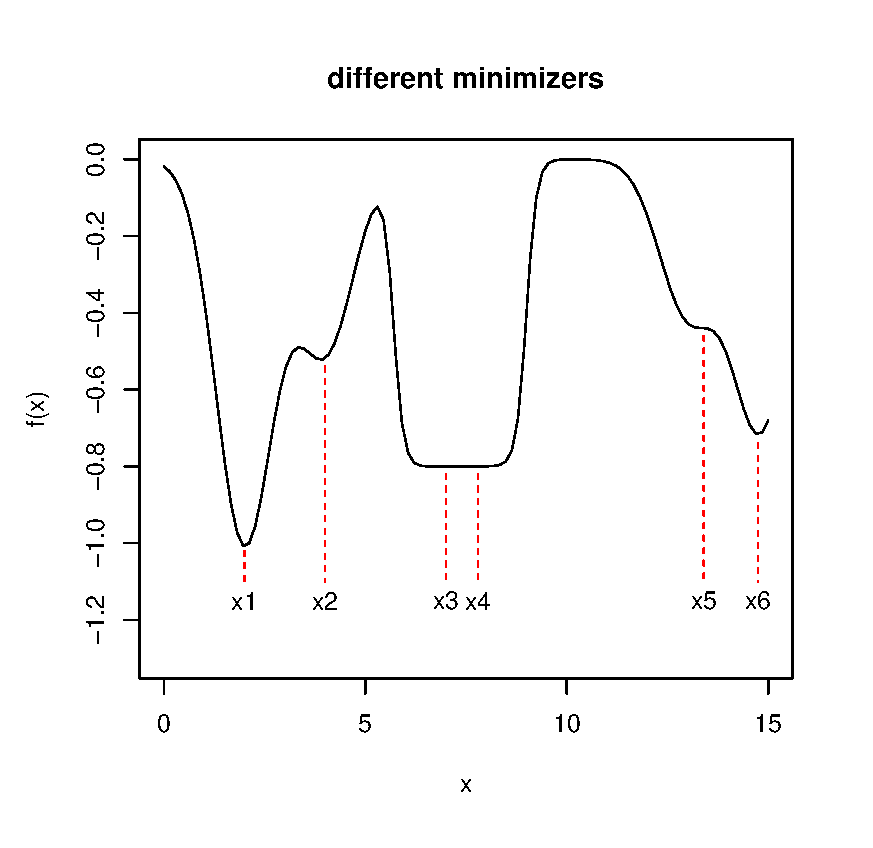
\includegraphics[width=3.0in]
		{02Background/opt/minimizers.png}
	\end{center}
	\caption[ค่าทำให้น้อยที่สุดต่าง ๆ]{ค่าทำให้น้อยที่สุดต่าง ๆ ของปัญหา $\mathrm{min}_x \; f(x)$. ค่าน้อยที่สุดของ $x$ หรือ $x_{\min} = -\infty$ แต่ค่าทำให้น้อยที่สุด $x^\ast = x_1$. ค่า $x_2, x_3, x_4, x_5, x_6$ เป็นค่าทำให้น้อยที่สุดท้องถิ่น. }
	\label{fig: opt minimizers}
\end{figure}
%



\subsection{การแก้ปัญหาด้วยวิธีลงเกรเดียนต์}
\label{sec: opt grad desc}
\index{thai}{วิธีลงเกรเดียนต์}
\index{english}{gradient descent algorithm}
\index{english}{optimization!gradient descent algorithm}
\index{thai}{การหาค่าดีที่สุด!วิธีลงเกรเดียนต์}

ศาสตร์\textit{การหาค่าดีที่สุด}นั้นกว้างขวาง
และมีการประยุกต์ใช้ที่หลากหลาย.
สำหรับการประยุกต์ใช้กับงาน\textit{การรู้จำรูปแบบ}
และ\textit{การเรียนรู้ของเครื่อง}
ลักษณะปัญหา มักจะถูกตีกรอบออกมาให้ตัวแปรตัดสินใจ $\bm{v} \in \mathbb{R}^n$ เมื่อ $n$ เป็นจำนวนเต็มมีค่าตั้งแต่หนึ่งขึ้นไป
และฟังก์ชันจุดประสงค์ 
%$g: \mathbb{R}^n \mapsto \mathbb{R}$ 
%โดยฟังก์ชัน 
$g$ เป็น\textit{ฟังก์ชันที่สามารถหาอนุพันธ์ได้} (differentiable function).
การมีฟังก์ชันจุดประสงค์ที่สามารถหาอนุพันธ์ได้
ช่วยให้สามารถใช้ขั้นตอนวิธีแก้ปัญหาค่าน้อยที่สุด
ที่มีประสิทธิภาพได้.

\textbf{วิธีลงเกรเดียนต์} (gradient descent algorithm) เป็น\textit{ขั้นตอนวิธี} (algorithm) สำหรับปัญหาค่าน้อยที่สุด.
\textit{วิธีลงเกรเดียนต์}เป็นขั้นตอนวิธีที่เรียบง่าย และใช้ได้ผลดี โดยเฉพาะกับปัญหาขนาดไม่ใหญ่มาก.
แนวคิดของ\textit{วิธีลงเกรเดียนต์} 
คือ
การใช้ค่าเกรเดียนต์
ช่วยในการหาค่าของ\textit{ตัวแปรตัดสินใจ}
โดย การเริ่มต้นด้วย
\textit{ค่าของตัวแปรตัดสินใจ} ค่าหนึ่ง
และคำนวณค่าเกรเดียนต์ ณ จุดนั้นออกมา
แล้วใช้ค่าเกรเดียนต์ที่ได้ บอกทิศทางในการปรับค่าของ\textit{ตัวแปรตัดสินใจ} ว่าควรปรับเพิ่มหรือลด มากน้อยเท่าไร 
ดำเนินการปรับค่าตัวแปรตัดสินใจ
และวนทำไปเรื่อย ๆ 
จนพบจุดที่เป็น\textit{ค่าทำให้น้อยที่สุด}.

เกรเดียนต์ 
ซึ่งเป็นอนุพันธ์ของฟังก์ชันจุดประสงค์ต่อตัวแปรตัดสินใจ
จะบอกอัตราการเปลี่ยนค่าของฟังก์ชันจุดประสงค์
เมื่อตัวแปรตัดสินใจเพิ่มค่าขึ้น.
ดังนั้นหาก{เกรเดียนต์}เป็นบวกและมีค่ามาก
นั่นหมายถึง 
ถ้าเพิ่มค่าตัวแปรตัดสินใจขึ้น
แล้วฟังก์ชันจุดประสงค์จะมีค่าเพิ่มขึ้นมาก.
หากค่าของ{เกรเดียนต์}เป็นบวกแต่มีขนาดเล็ก
การเพิ่มค่าตัวแปรตัดสินใจขึ้น
จะไปเพิ่มค่าฟังก์ชันจุดประสงค์ขึ้น แต่ไม่มาก
และหากเกรเดียนต์เป็นลบ
เมื่อเพิ่มค่าตัวแปรตัดสินใจขึ้น
ค่าฟังก์ชันจุดประสงค์จะลดลง.
ดังนั้นเกรเดียนต์จึงสามารถใช้เป็นเสมือนเงื่อนงำ 
ที่บอกทิศทางที่จะปรับค่า\textit{ตัวแปรตัดสินใจ} เพื่อลดค่าฟังก์ชันจุดประสงค์ลงไปเรื่อย ๆ
จนไปถึงค่าฟังก์ชันจุดประสงค์ที่น้อยที่สุดได้.
สมการ~\ref{eq: opt gd} 
แสดงการคำนวณค่าตัวแปรตัดสินใจ
ด้วยวิธีลงเกรเดียนต์
\begin{eqnarray}
\bm{v}^{(k+1)}
&=&
\bm{v}^{(k)} - \alpha \nabla g(\bm{v}^{(k)})
\label{eq: opt gd}
\end{eqnarray}
เมื่อ 
ตัวแปร $\bm{v}^{(k+1)}$
เป็นค่าใหม่ของตัวแปรตัดสินใจ (ที่ได้จากการคำนวณครั้งที่ $k+1$)
และ
ตัวแปร $\bm{v}^{(k)}$
เป็นค่าเดิมของตัวแปรตัดสินใจ (ที่ได้จากการคำนวณครั้งที่ $k$)
และ
เกรเดียนต์
$\nabla g(\bm{v}^{(k)})$
คือค่าเกรเดียนต์ของฟังก์ชันจุดประสงค์
ที่ค่าเดิมของตัวแปรตัดสินใจ 
(ค่าตัวแปรตัดสินใจที่ได้จากการคำนวณครั้งที่ $k$)
และค่าสเกล่าร์ $\alpha > 0$ เรียกว่า \textbf{ขนาดก้าว} (step size)
\index{thai}{ขนาดก้าว}
\index{english}{step size}
เป็นค่าที่ใช้ควบคุมอัตราเร็วในการปรับค่าของตัวแปรตัดสินใจ.

แนวคิดนี้ อุปมาเหมือน คนที่อยู่บนยอดเขาสูง 
ที่หมอกลงมากจนมองอะไรไม่เห็น 
และต้องการกลับบ้านที่อยู่พื้นล่าง.
เปรียบฟังก์ชันจุดประสงค์
เป็นเหมือนระดับความสูงของพื้นที่ ณ จุดที่ยืนอยู่
และตัวแปรตัดสินใจเป็นเหมือนตำแหน่งเส้นรุ้งเส้นแวง (latitude-longitude location) ณ จุดที่ยืนอยู่
ตัวแปร $\bm{v}^{(k)}$ ก็เสมือนตำแหน่งที่ยืนอยู่ปัจจุบัน
และเกรเดียนต์ $\nabla g(\bm{v}^{(k)})$ ก็เหมือนความชัน
ณ ตำแหน่งที่ยืนปัจจุบัน
ที่บอกว่าทิศทางไหนที่รู้สึกว่าพื้นชันขึ้น.
ถ้าต้องการกลับบ้าน หรือไปตำแหน่งที่ระดับความสูงที่ต่ำที่สุด
วิธีคือ ขยับจากจุดที่ยืนปัจจุบันไปจุดใหม่
โดยขยับไปในทิศทางลง (ซึ่งคือ ทิศทางตรงข้ามกับทิศที่พื้นชันขึ้น ได้แก่ ทิศ $-\nabla g(\bm{v}^{(k)})$)
โดยต้องค่อย ๆ เดิน ค่อย ๆ ก้าวเล็ก ๆ เพราะถ้าก้าวยาวเกินไป อาจก้าวข้ามทางเดินลงเขาแคบ ๆ ที่จะกลับบ้านได้ และ\textit{ขนาดก้าว} $\alpha$ ก็เป็นค่าที่ใช้คุมไม่ให้ก้าวยาวเกินไป
หลังจากก้าวไปแล้ว
ตอนนี้ ตำแหน่งที่ยืนก็จะเปลี่ยนใหม่เป็น $\bm{v}^{(k+1)}$
และก็ขยับแบบนี้อีก ทำซ้ำเรื่อย ๆ จนกลับถึงบ้าน.

\paragraph{ตัวอย่าง.}
การหา\textit{ค่าทำให้น้อยที่สุด}ของ $f(x) = - e^{ - (x-5)^2 }$ ด้วยวิธีลงเกรเดียนต์.
%
	\begin{itemize}
		\item
	เริ่มต้นด้วยการเลือกจุดเริ่มต้น สมมติเลือก $x^{(0)} = 6.5$ และเลือกใช้ค่าขนาดก้าว
	สมมติเลือกเป็น $\alpha = 0.5$.
	เกรเดียนต์สามารถวิเคราะห์การคำนวณไว้ได้
		\begin{eqnarray}
		\nabla f(x) &=& 
		\frac{d f(x)}{d x} = - e^{ - (x-5)^2 } \cdot (-2 x + 10).
		\nonumber   
		\end{eqnarray} 
%	
		\item ปรับค่าตัวแปรตัดสินใจ ตามสมการ~\ref{eq: opt gd}
		\\ 
		\begin{eqnarray}
		%(k=1) 
		&\;& \mbox{การคำนวณครั้งแรก } (k=1)
		\nonumber \\
		x^{(1)} &=& x^{(0)} - (0.5) \cdot \nabla f (x^{(0)})
%		\nonumber \\
%		&=& 
		= 6.5 - (0.5) \cdot \nabla f (6.5) 
		\nonumber \\ 
		&=& 6.5 - (0.5) \cdot \left(- e^{ - (6.5-5)^2 } \cdot (-2 \cdot (6.5) + 10) \right) 
		= 6.3419.
		\nonumber
\\		
%		\end{eqnarray}
%		\begin{eqnarray}
		%(k=2) 
		&\;& \mbox{การคำนวณที่สอง } (k=2)
\nonumber \\
		x^{(2)} &=& x^{(1)} - (0.5) \cdot \nabla f (x^{(1)})
%\nonumber \\
%&=& 
 = 6.3419 - (0.5) \cdot \nabla f (6.3419) = 6.1202
\nonumber
\\
%		\end{eqnarray}
%		\begin{eqnarray}	
%		&\;& \mbox{การคำนวณที่สาม } (k=3)
		&\;& \mbox{การคำนวณต่อ ๆ มา}
\nonumber \\
		x^{(3)} &=& 6.1202 - (0.5) \cdot \nabla f (6.1202) = 5.8009
\nonumber
%		\end{eqnarray}
%		\begin{eqnarray}	
%		&\;& \mbox{การคำนวณที่สี่ } (k=4)
%		&\;& \mbox{การคำนวณต่อ ๆ มา}
%\nonumber 
\\
x^{(4)} &=& 5.8009 - (0.5) \cdot \nabla f (5.8009) = 5.3792
\nonumber 
%\\
\end{eqnarray}
%
และ $x^{(5)} = 5.0508$;
$x^{(6)} = 5.0001$;
$x^{(7)} = 5.0000$;
$x^{(8)} = 5.0000$.
%\begin{eqnarray}	
%		&\;& \mbox{การคำนวณที่ห้า } (k=5)
%\nonumber \\
%		x^{(5)} &=& 5.0508   
%\end{eqnarray}
%\begin{eqnarray}	
%\nonumber \\
%		&\;& \mbox{การคำนวณที่หก } (k=6)
%\nonumber \\   
%x^{(6)} &=& 5.0001   
%\nonumber \\   
%		&\;& \mbox{การคำนวณที่เจ็ด } (k=7)
%\nonumber \\
%x^{(7)} &=& 5.0000   
%\nonumber \\   
%		&\;& \mbox{การคำนวณที่แปด } (k=8)
%\nonumber \\
%x^{(8)} &=& 5.0000   
%\nonumber
%		\end{eqnarray}
%		
		\item และผลลู่เข้าสู่ $x = 5$ ซึ่งคือ\textit{ค่าทำให้น้อยที่สุด}.
		ส่วน $f(5) = -1$ เป็นค่าฟังก์ชันจุดประสงค์ที่น้อยที่สุด 
		และค่าเกรเดียนต์ ณ จุดนี้คือ $\nabla f(5) = 0$.
	\hfill $\#$%$\square$
	\end{itemize}
%	
สังเกตว่า ที่ค่าทำให้น้อยที่สุด $x^\ast$ จะทำให้เกรเดียนต์ $\nabla f(x^\ast) = 0$
และนี่คือ ธรรมชาติ%
\footnote{%
	นี่คือ \textit{เงื่อนไขจำเป็นอันดับแรก} (First-Order Necessary Condition).
	ดู \cite{ChongZak2ndEd} สำหรับรายละเอียด.
}
ของ\textit{ค่าทำให้น้อยที่สุด}
ซึ่งคือ
ณ จุด\textit{ค่าทำให้น้อยที่สุด}
เกรเดียนต์จะมีค่าเป็นศูนย์%
\footnote{%
เกรเดียนต์ $\nabla f(x^\ast) = 0$
เป็นจริง 
ในกรณีทั่วไปของปัญหาค่าน้อยที่สุดแบบไม่มีข้อจำกัด.
หัวข้อ~\ref{sec: opt contrained opt} อภิปรายกรณีปัญหาค่าน้อยที่สุดแบบมีข้อจำกัด
และแบบฝึกหัด~\ref{ex: opt min problem piecewise} แสดงตัวอย่างกรณีพิเศษ
ที่  
ณ จุด\textit{ค่าทำให้น้อยที่สุด}
แต่ค่าเกรเดียนต์ไม่เป็นศูนย์.
}
ดังนั้น ถึงแม้จะคำนวณต่อ
ค่าของตัวแปรตัดสินใจก็จะยังคงติดอยู่ที่\textit{ค่าทำให้น้อยที่สุด}.

\paragraph{การใช้งานวิธีลงเกรเดียนต์.}
\textit{วิธีลงเกรเดียนต์} มี\textit{อภิมานพารามิเตอร์}
เป็นค่า\textit{ขนาดก้าว}.
\index{thai}{อภิมานพารามิเตอร์}
\index{thai}{พารามิเตอร์!อภิมาน}
\index{english}{meta-parameter}
\index{english}{hyper-parameter}
\index{english}{parameter!meta-}
\index{english}{parameter!hyper-}
%
\textbf{อภิมานพารามิเตอร์}
(meta-parameter หรือ hyper-parameter)
หมายถึง ปัจจัยระดับสูงของวิธีการคำนวณ แต่ละวิธี
ที่ผู้ใช้ต้องเลือกให้เหมาะสม.
สำหรับ\textit{วิธีลงเกรเดียนต์}
ผู้ใช้ต้องเลือกค่าของ\textit{ขนาดก้าว}.
ถ้าเลือกใช้\textit{ขนาดก้าว}ที่มีค่าเล็กพอ
\textit{วิธีลงเกรเดียนต์}
จะรับประกัน\textit{การลู่เข้าได้}%
\footnote{%
\textit{วิธีลงเกรเดียนต์}
รับประกันการลู่เข้าสู่ค่าทำน้อยที่สุดท้องถิ่น
เมื่อเลือกใช้ขนาดก้าวที่มีค่าเล็กพอ
แต่ไม่ได้รับประกันว่า
จะเจอค่าทำน้อยที่สุดทั่วหมด
หรือไม่ได้รับประกันว่า จะไม่ไปติดอยู่\textit{จุดอานม้า} เป็นต้น.
}.
\textbf{การลู่เข้า} (convergence)
\index{english}{convergence}
\index{thai}{การลู่เข้า}
หมายถึง พฤติกรรมที่ดีของผลการคำนวณ
สำหรับ\textit{การคำนวณลักษณะการวนซ้ำขัดเกลา} (iterative refinement computation)
นั่นคือ
ค่าของผลการคำนวณของแต่ละรอบคำนวณ
มีการเปลี่ยนแปลงน้อยลง เมื่อรอบการคำนวณเพิ่มมากขึ้น
อาจกล่าวได้ว่า
การลู่เข้าคือพฤติกรรมที่ ผลลัพธ์จากการคำนวณเปลี่ยนแปลงค่าเข้าหา(ลู่เข้าหา)ค่าใดค่าหนึ่ง ในลักษณะคงที่
เมื่อรอบการคำนวณเพิ่มมากขึ้น.

\textit{ขนาดก้าว}ที่ใหญ่เกินไป อาจทำให้การคำนวณล้มเหลวได้
แต่\textit{ขนาดก้าว}ที่เล็กเกินไป อาจทำให้ต้องทำการคำนวณหลายรอบมาก ๆ 
ซึ่งมีผลให้ใช้เวลาในการคำนวณนาน
(ดูแบบฝึกหัด~\ref{ex: opt gd step size} ประกอบ).
ในทางปฏิบัติ
เพื่อให้ไม่เสียเวลาคำนวณมากเกินไป
\textbf{เงื่อนไขการจบ}การคำนวณ (terminating condition)
มักถูกใช้ประกอบ.
\index{english}{terminating condition}
\index{thai}{เงื่อนไขการจบ}
%
\textit{เงื่อนไขการจบ}ที่นิยมใช้กับ\textit{วิธีลงเกรเดียนต์}
ได้แก่ เงื่อนไข\textit{จำนวนรอบสูงสุด} (maximum number of iterations)
และ
เงื่อนไข\textit{ความคลาดเคลื่อนยินยอม} (tolerance).

เงื่อนไข\textit{จำนวนรอบสูงสุด}
จะกำหนดจำนวนรอบที่จะหยุดทำการคำนวณ
ไม่ว่าการคำนวณนั้น จะดำเนินไปถึงสิ้นสุดหรือไม่ จะได้\textit{ค่าทำให้น้อยที่สุด}แล้วหรือไม่.
นั่นคือ กำหนด
$\bm{v}^{(k+1)} = \bm{v}^{(k)} - \alpha \nabla g (\bm{v}^{(k)})$ สำหรับ $k = 1, \ldots, N_{\max}$
เมื่อ $N_{\max}$ คือจำนวนรอบคำนวณที่มากที่สุด
และการใช้เงื่อนไขนี้ จะทำให้ผู้ใช้ต้องกำหนด\textit{จำนวนรอบสูงสุด}นี้ด้วย.
ดังนั้น\textit{อภิมานพารามิเตอร์}
จะมี\textit{จำนวนรอบสูงสุด}ขึ้นอีกตัว.

\textit{เงื่อนไขความคลาดเคลื่อนยินยอม}
กำหนดค่าความคลาดเคลื่อนที่ยอมรับได้ ซึ่งอาจเลือกใช้เงื่อนไข 
ขนาดของเกรเดียนต์
$\epsilon = \|\nabla g(\bm{v}^{(k+1)})\|$.
แบบฝึกหัด~\ref{ex: opt gd simple code}
แสดงตัวอย่างโปรแกรม\textit{วิธีลงเกรเดียนต์}อย่างง่าย
ที่ใช้\textit{เงื่อนไขการจบ}แค่\textit{จำนวนรอบสูงสุด}.
แบบฝึกหัด~\ref{ex: opt gd termination code} 
แสดงตัวอย่างโปรแกรม\textit{วิธีลงเกรเดียนต์}ที่ใช้\textit{เงื่อนไขคลาดเคลื่อนยินยอม}.

\textit{วิธีลงเกรเดียนต์}ประยุกต์ใช้ได้ง่าย
ต้องการแค่เกรเดียนต์ และค่าเริ่มต้น.
ค่าเริ่มต้นก่อนการคำนวณของตัวแปรตัดสินใจ 
อาจเป็นค่าใดก็ได้%
\footnote{%
\textit{วิธีลงเกรเดียนต์}ทนทานต่อค่าเริ่มต้นต่าง ๆ
ในแง่ที่ว่า โดยทั่วไปแล้ว (ถ้าปัญหาไม่ยากเกินไป)
\textit{วิธีลงเกรเดียนต์}จะสามารถหา\textit{ค่าทำให้น้อยที่สุด}ได้
แม้เลือกค่าเริ่มต้นต่างกัน
แต่การเลือกค่าเริ่มต้นที่ดี
จะช่วยให้\textit{วิธีลงเกรเดียนต์}ทำงานได้เร็วขึ้น
และสำหรับหลาย ๆ กรณี
ค่าเริ่มต้นต่างกันอาจนำไปสู่\textit{ค่าทำให้น้อยที่สุดท้องถิ่น}คนละตัว (กรณีปัญหา\textit{หลายภาวะ} multi-modal problem ดูแบบฝึกหัด~\ref{ex: opt gd init} เพิ่มเติม)
หรือสำหรับบางกรณี
ค่าเริ่มต้นบางค่า อาจทำให้\textit{วิธีลงเกรเดียนต์}ไม่สามารถทำงานได้เลย.
ดูแบบฝึกหัด~\ref{ex: opt gd init} ประกอบ.
}
แต่โดยทั่วไป มักนิยมใช้\textbf{การกำหนดค่าเริ่มต้น} (initialization) ให้กับ\textit{ตัวแปรตัดสินใจ}
ด้วยค่าที่สุ่มขึ้นมา.
(ดูแบบฝึกหัด~\ref{ex: opt gd random.norm init})

ปัญหาที่ตัวแปรตัดสินใจมีหลาย ๆ ตัว 
สามารถใช้วิธีลงเกรเดียนต์ได้
โดยการจัดหลาย ๆ ตัวแปรตัดสินใจ 
เข้ามารวมกันเป็นเวกเตอร์ตัวแปรตัดสินใจเวกเตอร์เดียว
และวิธีลงเกรเดียนต์เตรียมการมาสำหรับกรณีนี้อยู่แล้ว 
(สมการ~\ref{eq: opt gd}).
สังเกตว่า ตัวแปรตัดสินใจเขียนเป็นเวกเตอร์
และอัตราการเปลี่ยนก็ใช้เกรเดียนต์
แต่การนำ\textit{วิธีลงเกรเดียนต์}
ไปเขียนโปรแกรมเพื่อทำงานกับเวกเตอร์
จะต้องระวังเรื่องของตัวแปรเป็นพิเศษ. 
(ดูแบบฝึกหัด~\ref{ex: opt gd vec code} ประกอบ)
นอกจากนั้น เพื่อช่วยให้สามารถตรวจสอบความก้าวหน้า
ในการหา\textit{ค่าทำให้น้อยที่สุด}ได้อย่างมีประสิทธิภาพ ควรตรวจสอบ\textit{ค่าฟังก์ชันจุดประสงค์}ทุก ๆ รอบคำนวณ.
ตัวอย่างต่อไปนี้ แสดงการคำนวณของ\textit{วิธีลงเกรเดียนต์} เมื่อตัวแปรตัดสินใจมีสองค่า.

%
\begin{figure}
	\begin{center}
		\begin{tabular}{cc}
			\includegraphics[width=3.0in]
			{02Background/opt/code_opt_2Dcontour.png}
			&
			\includegraphics[width=3.0in]
			{02Background/opt/code_opt_2Dpersp.png}\\\
			ก & ข	
		\end{tabular}
	\end{center}
	\caption[ภาพคอนทัวร์และภาพสามทัศนมิติของฟังก์ชันจุดประสงค์]{ภาพคอนทัวร์ (ก) และภาพสามทัศนมิติ (ข) ของฟังก์ชันจุดประสงค์ $g(\bm{v}) = -e^{-53-v_1^2 -2v_2^2-v_1 v_2 + 10 v_1 + 19 v_2}$}
	\label{fig: opt 2D}
\end{figure}

\paragraph{ตัวอย่าง เมื่อตัวแปรตัดสินใจเป็นเวกเตอร์.}
%จงใช้วิธีลงเกรเดียนต์ 
%เพื่อแก้
ปัญหา เช่น $\min_{\bm{v}} \; g$ เมื่อ
$\bm{v} =[v_1, v_2]^T$
และ
$g(\bm{v}) = -e^{-53-v_1^2 -2v_2^2-v_1 v_2 + 10 v_1 + 19 v_2}$
ซึ่งรูป~\ref{fig: opt 2D} แสดงฟังก์ชันจุดประสงค์ในรูปคอนทัวร์ (contour plot) และในรูปสามทัศนมิติ (3d perspective plot)
ปัญหานี้สามารถแก้ด้วยวิธีลงเกรเดียนต์ ดังนี้.

	\begin{itemize}
	\item
	เลือก\textit{อภิมานพารามิเตอร์}
	ได้แก่ ค่าขนาดก้าว $\alpha = 0.01$

	\item 
	เตรียมฟังก์ชันคำนวณเกรเดียนต์
	\begin{eqnarray}
	\nabla g(\bm{v}) &=& 
	\begin{bmatrix}
	\frac{\partial g}{\partial v_1} \\
	\frac{\partial g}{\partial v_2}
	\end{bmatrix}
	= 
	\begin{bmatrix}
g(\bm{v}) \cdot (-2 v_1 - v_2 + 10) \\
g(\bm{v}) \cdot (-4 v_2 - v_1 + 19)
\end{bmatrix}
= g(\bm{v}) \cdot 
\begin{bmatrix}
-2 v_1 - v_2 + 10
\\
-4 v_2 - v_1 + 19
\end{bmatrix}
	\nonumber .  
	\end{eqnarray} 
สังเกต ค่าฟังก์ชันจุดประสงค์ $g(\bm{v})$ เป็นสเกล่าร์
แต่ค่าเกรเดียนต์ $\nabla g(\bm{v})$ เป็นเวกเตอร์ ที่มีสัดส่วน (จำนวนส่วนประกอบ) เท่ากับสัดส่วนของตัวแปรตัดสินใจ $\bm{v}$.
	
\item สุ่มเลือกค่าเริ่มต้น สมมติว่าสุ่มได้ $\bm{v}^{(0)} = [2.5, 3.5]^T$

\item ปรับค่าตัวแปรตัดสินใจ ตามสมการ~\ref{eq: opt gd}
	\\ 
	\begin{eqnarray}
	%(k=1) 
	&\;& \mbox{การคำนวณครั้งแรก } (k=1)
	\nonumber \\
	\bm{v}^{(1)} &=& \bm{v}^{(0)} - (0.01) \cdot \nabla g (\bm{v}^{(0)})
	\nonumber \\
	&=& [2.5, 3.5]^T - 0.01 \cdot (-0.3679) \cdot [-2(2.5)-3.5+10, -4(3.5)-2.5+19]^T
	\nonumber \\
	&=& [2.5, 3.5]^T - 0.01 \cdot [-0.5518,
	-0.9197]^T = [2.506, 3.509]^T
\nonumber \\	
	&\;& \mbox{การคำนวณที่สอง } (k=2)
\nonumber \\		
	\bm{v}^{(2)} &=& \bm{v}^{(1)} - (0.01) \cdot \nabla g (\bm{v}^{(1)})
\nonumber \\	
&=& [2.506, 3.509]^T - 0.01 \cdot [-0.5615, -0.9326]^T = [2.511, 3.519]^T
\nonumber \\
	&\;& \mbox{การคำนวณที่สาม } (k=3)
	\nonumber \\
	\bm{v}^{(3)} &=& \bm{v}^{(2)} - (0.01) \cdot \nabla g (\bm{v}^{(2)})
\nonumber \\	
&=& [2.511, 3.519]^T - 0.01 \cdot [-0.5711, -0.9452]^T = [2.517, 3.528]^T
\nonumber 
	\nonumber
	\end{eqnarray}
	
	\item และเมื่อดำเนินการคำนวณต่อไป
	(ดูแบบฝึกหัด~\ref{ex: opt gd vec code} ประกอบ)
	จะพบว่า 
%	$\bm{v}^{(100)} = [2.928, 4.013]^T$,
%	$\bm{v}^{(200)} = [2.987, 4.005]^T$,
	$\bm{v}^{(300)} = [2.997, 4.001]^T$,
	$\bm{v}^{(400)} = [2.999, 4.000]^T$,
	$\bm{v}^{(500)} = [3.000, 4.000]^T$,
	$\bm{v}^{(600)} = [3.000, 4.000]^T$.
	ค่าของ $\bm{v}$ ปรับน้อยมาก ๆ จนถึงแทบไม่ปรับเลยในรอบคำนวณหลัง ๆ นี่คือ $\bm{v}$ ลู่เข้าหา $[3, 4]^T$.
	รูป~\ref{fig: opt gd 2D trajectory} แสดงการปรับค่าตัวแปรตัดสินใจ ในรูปเส้นทางบนภาพคอนทัวร์%
	\footnote{รูปเส้นทางบนภาพคอนทัวร์ เช่นนี้ สามารถแสดงได้เฉพาะกรณีที่ตัวแปรตัดสินใจ $\bm{v} \in \mathbb{R}^2$ หากตัวแปรตัดสินใจอยู่ในมิติปริภูมิที่ใหญ่ขึ้น การนำเสนอด้วยภาพจะทำได้ยากมาก.}
	ของฟังก์ชันจุดประสงค์.
	รูป~\ref{fig: opt gd 2D} แสดง \textit{ความก้าวหน้า} (progress) ของการดำเนินการหาค่าทำให้น้อยที่สุด.
	\hfill $\#$%$\square$
\end{itemize}

จากรูป~\ref{fig: opt gd 2D} 
ค่าของ\textit{ตัวแปรตัดสินใจ} $\bm{v}$ ทั้งสองค่า 
จะปรับเข้าหา $[3, 4]^T$
นั่นคือคำตอบลู่เข้า.
เมื่อดูที่จุดลู่เข้า  ดังที่ได้อภิปรายมาแล้ว
ขนาดของเกรเดียนต์จะเป็นศูนย์ที่\textit{จุดดีที่สุด} (optimal point)
\index{thai}{จุดที่ดีที่สุด}
\index{english}{optimal point}
ซึ่งเป็นจุดที่\textit{ตัวแปรตัดสินใจ}ปรับค่าไปอยู่ที่\textit{ค่าทำให้น้อยที่สุด}.
ขนาดของเกรเดียนต์จึงนิยมใช้เป็นเงื่อนไขในการจบโปรแกรม เพื่อไม่ต้องคำนวณมากรอบเกินไป เช่นกรณีนี้ จะเห็นว่าทำการคำนวณแค่ราว ๆ $500$ รอบก็เห็นการลู่เข้าชัดเจนแล้ว.
เมื่อดูที่ฟังก์ชันจุดประสงค์ (ภาพ Loss บนซ้าย) ค่าฟังก์ชันจุดประสงค์จะน้อยลงเรื่อย ๆ ถ้าเลือกค่า\textit{ขนาดก้าว}ไม่ใหญ่เกินไป.
พฤติกรรมการทำงานของ\textit{วิธีลงเกรเดียนต์}จะมีลักษณะเช่นนี้ คือ 
ค่าฟังก์ชันจุดประสงค์จะลดลง เมื่อรอบคำนวณเพิ่มขึ้น.
การดูค่าฟังก์ชันจุดประสงค์ต่อรอบคำนวณเช่นนี้
สะดวก เพราะสามารถตรวจสอบได้ ไม่ว่าตัวแปรตัดสินใจจะมีจำนวนเท่าใด
และถูกใช้เป็นแนวทางปฎิบติ
เพื่อติดตามความก้าวหน้า
และวิเคราะห์การทำงานของการแก้ปัญหาค่าน้อยที่สุด ว่าดำเนินการได้ดีมากน้อยเพียงใด.

%
\begin{figure}
	\begin{center}
		\includegraphics[width=0.75\textwidth]
		{02Background/opt/code_opt_2Dgd_trajectory.png}
	\end{center}
	\caption[เส้นทางการหาค่าทำให้น้อยที่สุด]{เส้นทางการหา\textit{ค่าทำให้น้อยที่สุด} จุดวงกลมสีดำแสดงจุดเริ่มต้น (ตำแหน่ง $[2.5, 3.5]^T$) และจุดดาวสีแดงแสดงจุดสุดท้าย (ตำแหน่ง $[3, 4]^T$). เส้นทางระหว่างจุดทั้งสอง คือค่าต่าง ๆ ที่ตัวแปรตัดสินใจถูกปรับตั้งแต่รอบคำนวณแรก ๆ ไปจนถึงรอบคำนวณท้าย ๆ.
	}
	\label{fig: opt gd 2D trajectory}
\end{figure}
%


%
\begin{figure}
	\begin{center}
		\includegraphics[width=0.75\textwidth]
		{02Background/opt/code_opt_2Dgd_progress.png}
	\end{center}
	\caption[ความก้าวหน้าในการหาค่าทำให้น้อยที่สุด]{\textit{ความก้าวหน้า}ในการหา\textit{ค่าทำให้น้อยที่สุด}. 
	ภาพบนซ้าย (\texttt{Loss}) แสดงค่าฟังก์ชันจุดประสงค์ต่อรอบการคำนวณ. 
	ภาพล่างซ้าย (\texttt{|grad|}) แสดงขนาดเกรเดียนต์ต่อรอบการคำนวณ.
	ขนาดเกรเดียนต์นิยมใช้เป็น\textit{เงื่อนไขการจบ} เพื่อลดเวลาคำนวณลง.
	ภาพขวาแสดงค่า\textit{ตัวแปรตัดสินใจ}ต่อรอบการคำนวณ ภาพบนแสดง $v_1$ และภาพล่างแสดง $v_2$.
    }
	\label{fig: opt gd 2D}
\end{figure}
%


%วิธีลงเกรเดียนต์นั้น นอกจากใช้งานได้ดีกับปัญหาค่าน้อยที่สุดแล้ว
%ยังใช้ได้ดีกับชีวิตด้วย
\begin{quote}
วิธีลงเกรเดียนต์:\\
``ไม่ว่าเราเริ่มต้นอยู่ที่ไหน ถ้าเราขยับไปทิศทางที่ดีขึ้นเรื่อย ๆ
\\
เราจะไปถึงจุดที่ดีที่สุดได้
เพียงต้องทำเรื่อย ๆ และไม่รีบเกินไป''
\end{quote}
\index{english}{quote!gradient descent}



\subsection{การหาค่าดีที่สุดแบบมีข้อจำกัด}
\label{sec: opt contrained opt}
\index{english}{constrained optimization}
\index{thai}{การหาค่าดีที่สุดแบบมีข้อจำกัด}
\index{english}{optimization!constrained}
\index{thai}{การหาค่าดีที่สุด!แบบมีข้อจำกัด}

\textit{การหาค่าดีที่สุด}ที่ได้อภิปรายมา
ค่าของตัวแปรตัดสินใจเป็นค่าจำนวนจริงใด ๆ
ซึ่งเขียนเป็นสัญกรณ์ทั่ว ๆ ไป $\mathrm{min}_{\bm{v}} g(\bm{v})$ โดย $\bm{v} \in \mathbb{R}^n$ เมื่อ $n$ เป็นจำนวนเต็มที่มีค่าตั้งแต่หนึ่งเป็นต้นไป
\textit{การหาค่าดีที่สุด}แบบนี้ 
ไม่ได้มีเงื่อนไขจำกัดค่าของตัวแปรตัดสินใจ (นอกจากเป็นจำนวนจริง)
และ\textit{การหาค่าดีที่สุด}แบบนี้ จะเรียกว่า
\textbf{การหาค่าดีที่สุดแบบไม่มีข้อจำกัด} (unconstrained optimization).

กรณีที่มีข้อจำกัดของค่าของตัวแปรตัดสินใจ
จะเรียกว่า
\textbf{การหาค่าดีที่สุดแบบมีข้อจำกัด} (constrained optimization)
และจะใช้สัญกรณ์ เพื่อระบุข้อจำกัดอย่างชัดเจน เช่น
\begin{eqnarray}
\underset{\bm{v}}{\mathrm{minimize}} & g(\bm{v})
\nonumber \\
\mbox{subject to} & \bm{v} \in \Omega 
\label{eq: opt contrained opt}
\end{eqnarray}
เมื่อ $\bm{v} \in \mathbb{R}^n$ เป็นตัวแปรตัดสินใจ
ฟังก์ชัน $g: \mathbb{R}^n \rightarrow \mathbb{R}$ เป็นฟังก์ชันจุดประสงค์
และเซต $\Omega$ เป็นเซตย่อยของ $\mathbb{R}^n$ ที่ระบุค่าของตัวแปรตัดสินใจในช่วงที่สนใจ หรือกลุ่มค่าที่ยอมรับได้.
ค่าคำตอบของ $\bm{v}$ ที่ได้จะต้องอยู่ในเซตย่อยนี้.
เซต $\Omega$ นี้ เรียกว่า \textbf{เซตข้อจำกัด} (constraint set หรือ เซตที่เป็นไปได้ feasible set).
กรณีที่ $\Omega = \mathbb{R}^n$
ปัญหาในกรณีนี้จะเป็น
\textit{การหาค่าดีที่สุดแบบไม่มีข้อจำกัด}.
สัญกรณ์~\ref{eq: opt contrained opt} อาจเขียนย่อเป็น $\mathrm{min}_{\bm{v}} \; g(\bm{v}) \; \mbox{s.t.} \; \bm{v} \in \Omega$.

จากตัวอย่าง การหาอุณหภูมิบ่มทุเรียน ถ้ากำหนดว่า อุณหภูมิบ่มต้องอยู่ในช่วง $30$ ถึง $80$ องศาเซลเซียส (เพราะว่าเตาบ่มที่มี ทำอุณหภูมิได้ในช่วงแค่นั้น)
ปัญหานี้จะเป็น\textit{การหาค่าดีที่สุดแบบมีข้อจำกัด}
และอาจเขียนเป็น สัญกรณ์ $\mathrm{max}_t \; \mathrm{sugar}(t) \; \mbox{s.t.} \; 30 \leq t \leq 80$
เมื่อ $t$ แทนอุณหภูมิบ่มในหน่วยองศาเซลเซียส
ฟังก์ชัน $\mathrm{sugar}$ ประเมินระดับน้ำตาลที่ได้ จากการบ่มด้วยอุณหภูมิ $t$
และข้อจำกัด $30 \leq t \leq 80$ ระบุค่าของ $t$ ที่ใช้ได้ว่า อยู่ในช่วง $30$ ถึง $80$.
(ปัญหาค่ามากที่สุดนี้ เทียบเท่า
ปัญหาค่าน้อยที่สุด
$\mathrm{min}_t \; -\mathrm{sugar}(t) \; \mbox{s.t.} \; 30 \leq t \leq 80$
)

\paragraph{ค่าทำให้น้อยที่สุดท้องถิ่น และค่าทำให้มากที่สุดทั่วหมด.}
ในกรณีที่มีข้อจำกัด ค่าของตัวแปรตัดสินใจจะพิจารณาจากค่าที่\textit{เป็นไปได้} (feasible) เท่านั้น.
\textit{ค่าทำให้น้อยที่สุดท้องถิ่น}
คือ ค่าของตัวแปรตัดสินใจ ที่ทำให้ฟังก์ชันจุดประสงค์มีค่าน้อยกว่าหรือเท่ากับค่าฟังก์ชันจุดประสงค์ของค่าที่\textit{เป็นไปได้}บริเวณรอบ ๆ.
นั่นคือ
%\footnote{
%	สัญกรณ์ $\rho_1 \subset \rho_2$ บอกว่า เซต $\rho_1$ เป็นเซตย่อยของ $\rho_2$.
%	สัญกรณ์ $\rho_1 \setminus \rho_2$ เป็นการดำเนินการลบสมาชิก โดยผลลัพธ์คือ สมาชิกทุกตัวในเซต $\rho_1$ ที่ไม่ได้เป็นสมาชิกของเซต $\rho_2$.
%} 
ถ้ากำหนดให้ $g: \mathbb{R}^n \rightarrow \mathbb{R}$ เป็นฟังก์ชันค่าจริง 
ที่นิยามสำหรับเซต $\Omega \subset \mathbb{R}^n$
แล้ว จุด $\bm{v}^\ast \in \Omega$ เป็น\textit{ค่าทำให้น้อยที่สุดท้องถิ่น} ของฟังก์ชัน $g$ บนเซต $\Omega$ ถ้ามีค่า $\epsilon > 0$ ที่ $g(\bm{v}) \geq g(\bm{v}^\ast)$ สำหรับทุกค่าของ $\bm{v} \in \Omega \setminus \{ \bm{v}^\ast \}$
และ $\|\bm{v} - \bm{v}^\ast\| < \epsilon$.
ส่วน\textit{ค่าทำให้น้อยที่สุดทั่วหมด}
คือ ค่าของตัวแปรตัดสินใจ ที่ทำให้ฟังก์ชันจุดประสงค์มีค่าน้อยกว่าหรือเท่ากับค่าฟังก์ชันจุดประสงค์ของค่าที่\textit{เป็นไปได้}อื่น ๆ ทุกค่า.
นั่นคือ
จุด $\bm{v}^\ast \in \Omega$ จะเป็น\textit{ค่าทำให้น้อยที่สุดทั่วหมด}ของฟังก์ชัน $g$ บนเซต $\Omega$ ถ้า $g(\bm{v}) \geq g(\bm{v}^\ast)$ สำหรับ ทุกค่าของ $\bm{v} \in \Omega \setminus \{ \bm{v}^\ast \}$.

\paragraph{วิธีแก้ปัญหาค่าน้อยที่สุดแบบมีข้อจำกัด.}
มีสองแนวทางหลักที่ทั่วไปนิยมใช้แก้ปัญหาค่าน้อยที่สุดแบบมีข้อจำกัด คือ
\textit{แนวทางการแปลงมุมมอง}
และ\textit{แนวทางการลงโทษ}.
\index{english}{constrained optimization}
\index{english}{optimization!constrained}
\index{english}{constrained optimization!projection}
\index{english}{constrained optimization!penalty}
\index{thai}{การหาค่าดีที่สุดแบบมีข้อจำกัด!แนวทางการแปลงมุมมอง}
\index{thai}{การหาค่าดีที่สุดแบบมีข้อจำกัด!แนวทางการลงโทษ}

\textbf{แนวทางการแปลงมุมมอง} (projection approach)
จะใช้ฟังก์ชัน $F: \mathbb{R}^n \rightarrow \Omega$ เพื่อแปลงค่าของตัวแปรตัดสินใจมาเป็น\textit{ค่าที่เป็นไปได้}.
ตัวอย่าง เช่น เมื่อใชักับ\textit{วิธีลงเกรเดียนต์} อาจทำโดย
\begin{eqnarray}
\bm{v}^{(k+1)} = F \left( \bm{v}^{(k)} - \alpha \cdot \nabla g(\bm{v}^{(k)}) \right)
\label{eq: opt const projection} 
\end{eqnarray}
ในทางปฏิบัติแล้ว 
ฟังก์ชันแปลง $F$ นี้
อาจจะยากที่หา หรือยากที่จะคำนวณ
ในหลาย ๆ สถานการณ์.
งาน\textit{การเรียนรู้ของเครื่อง} มักนิยมใช้\textit{แนวทางการลงโทษ}มากกว่า.

\textbf{แนวทางการลงโทษ}
(penalty approach)
\index{english}{penalty method}
\index{thai}{วิธีการลงโทษ}
จะใช้การลงโทษ
เมื่อค่า\textit{ตัวแปรตัดสินใจ}ไม่อยู่ใน\textit{เซตข้อจำกัด}
โดยการปรับกรอบปัญหาจากเดิม $\min_{\bm{v}} g(\bm{v}) \; \mbox{s.t.} \; \bm{v} \in \Omega$
ไปเป็นกรอบปัญหาใหม่
\begin{eqnarray}
\underset{\bm{v}}{\mathrm{min}} \; g(\bm{v}) + \lambda P(\bm{v})
\label{eq: opt const penalty}
\end{eqnarray}
เมื่อ $\lambda \in \mathbb{R}$ 
เป็น\textbf{พารามิเตอร์ลงโทษ} (penalty parameter) ซึ่งนิยมเรียกว่า \textit{ลากรานจ์พารามิเตอร์} (Lagrange parameter)
\index{english}{Lagrange parameter}
\index{thai}{ลากรานจ์พารามิเตอร์}
และฟังก์ชัน $P: \mathbb{R}^n \rightarrow [0, \infty)$ เป็น\textit{ฟังก์ชันต่อเนื่อง} (continuous function)
เรียกว่า
\textbf{ฟังก์ชันลงโทษ} (penalty function)
\index{thai}{ฟังก์ชันลงโทษ}
\index{english}{penalty function}
โดย 
\textit{ฟังก์ชันลงโทษ}จะมีค่าเป็นศูนย์
เมื่อค่าตัวแปรตัดสินในอยู่ในเซตข้อจำกัด
นั่นคือ $P(\bm{v}') = 0$ สำหรับ $\bm{v}' \in \Omega$.

%ตัวอย่าง เช่นปัญหาบ่มทุเรียน
%$\min_t - \mathrm{sugar}(t) \; \mbox{s.t.} \; t \leq 80$
%ก็อาจจะถูกตีกรอบใหม่ตามแนวทางการลงโทษได้เป็น
%$\min_t - \mathrm{sugar}(t) + \lambda P_o (t)$
%เมื่อ

% np.sin(x)/(1 + x**2)
ตัวอย่างเช่น ปัญหา $\min_x \sin (x) /(1 + x^2) \; \mbox{s.t.} \; x \geq 0$.
รูป~\ref{fig: opt constrained problem} แสดงฟังก์ชันจุดประสงค์ 
%$\sin (x) /(1 + x^2)$
และแสดงส่วนที่ไม่ผ่านเงื่อนไขด้วยแรเงาสีเทา.
รูปแสดงให้เห็นว่า จุดที่ทำให้ค่าฟังก์ชันจุดประสงค์น้อยที่สุด มีค่าเป็นลบ แต่จุดนี้ละเมิดข้อจำกัด และใช้เป็นคำตอบไม่ได้.
การหาคำตอบด้วยวิธีลงโทษ
อาจเลือกใช้ฟังก์ชัน
\begin{eqnarray}
P(x) = \left \{ 
     \begin{array}{l l}
0 & \quad \mbox{เมื่อ} \quad x \geq 0, \\
-x & \quad \mbox{เมื่อ} \quad x < 0.
\end{array} 
\right.
\label{eq: opt const penalty function}
\end{eqnarray}
ซึ่งเป็นฟังก์ชันต่อเนื่อง (ทำให้สามารถหาอนุพันธ์ได้ และสามารถใช้วิธีแก้ปัญหา เช่น วิธีลงเกรเดียนต์ได้)
และฟังก์ชัน $P$ ลงโทษค่าที่ละเมิดข้อจำกัดตามปริมาณที่ละเมิด.
รูป~\ref{fig: opt penalty function} แสดงค่าของฟังก์ชันลงโทษในสมการ~\ref{eq: opt const penalty function}
และเมื่อนำฟังก์ชันลงโทษนี้
ไปใช้ร่วมกับฟังก์ชันจุดประสงค์
ฟังก์ชันที่ปรับใหม่จะเปลี่ยนพฤติกรรมไป
ดังแสดงในรูป~\ref{fig: opt penalized loss}.

วิธีใช้การลงโทษนี้ ก็คือ
การเปลี่ยนจาก\textit{ปัญหาแบบมีข้อจำกัด}
กลับมาเป็น\textit{ปัญหาแบบไม่มีข้อจำกัด}
โดย
การดัดแปลงฟังก์ชันจุดประสงค์ใหม่
เพื่อให้คำตอบ 
อยู่ในช่วงค่าที่\textit{เป็นไปได้}.
ดังนั้น ขั้นตอนการหาคำตอบต่อไป ก็สามารถดำเนินการได้
โดยใช้วิธีแก้ปัญหา แบบเดียวกับ\textit{ปัญหาแบบไม่มีข้อจำกัด}. % เช่น วิธีลงเกรเดียนต์ เป็นต้น.

รูป~\ref{fig: opt penalized loss} แสดงให้เห็นว่า
เมื่อ
ค่าของ\textit{ลากรานจ์พารามิเตอร์}ใหญ่มากพอ
\textit{ค่าทำน้อยที่สุด}ของฟังก์ชันจุดประสงค์ใหม่
จะถูกบังคับให้อยู่ในช่วงค่าที่\textit{เป็นไปได้}.
กลไกการทำงานของการลงโทษ คือ
การลงโทษจะทำให้
คำตอบของ\textit{ปัญหาค่าน้อยที่สุด}ใหม่ ที่รวม\textit{การลงโทษ}เข้าไป จะเป็น%
\footnote{%
กำหนดให้ $\bm{v}^{(k)}$ เป็นคำตอบของปัญหาที่มีการลงโทษด้วยค่า $\lambda_k$ 
และฟังก์ชันจุดประสงค์เดิม $g$ เป็นฟังก์ชันต่อเนื่อง
และ $\lambda_k \rightarrow \infty$
เมื่อ $k \rightarrow \infty$
แล้ว
\textit{ลิมิต} (limit) ของลำดับที่ลู่เข้า $\{ \bm{v}^{(k)} \}$ จะเป็นคำตอบของ\textit{ปัญหาแบบมีข้อจำกัด}เดิม. 
ดู \cite{ChongZak2ndEd} สำหรับรายละเอียด.
}%
คำตอบของ\textit{ปัญหาค่าน้อยที่สุดแบบมีข้อจำกัด}เดิม
เมื่อ\textit{ลากรานจ์พารามิเตอร์}มีค่าใหญ่มากพอ.

ในทางปฏิบัติ
การแก้ปัญหาด้วยวิธีลงโทษ จะเลือกค่าของ\textit{ลากรานจ์พารามิเตอร์}มาค่าหนึ่ง และดำเนินการแก้ปัญหา
แล้วตรวจสอบค่าคำตอบที่ได้ ว่าอยู่ภายใต้ข้อจำกัดหรือไม่
ถ้าคำตอบที่ได้ อยู่ภายใต้ข้อจำกัด นี่ก็คือ
คำตอบของปัญหาที่ใช้ได้.
แต่ถ้าคำตอบที่ได้ ไม่อยู่ภายใต้ข้อจำกัด
จะต้องเพิ่มค่าของ\textit{ลากรานจ์พารามิเตอร์}ขึ้น และดำเนินการแก้ปัญหาอีก และทำเช่นนี้ เพิ่มค่า\textit{ลากรานจ์พารามิเตอร์}ขึ้น
จนกว่าจะได้คำตอบที่อยู่ภายใต้ข้อจำกัด.


%นั่นคือ
%ถ้ากำหนดให้ 
%$\min_{\bm{v}} g(\bm{v}) 
%\mbox{ s.t. } \bm(v) \in \Omega$
%เป็นปัญหาแบบมีข้อจำกัด
%และ\textit{ปัญหาที่ถูกลงโทษ} (penalized problem) 
%ตีกรอบปัญหาเป็น 
%$\min_{\bm{v}} g(\bm{v}) + \lambda P(\bm(v))$
%เมื่อ $P(\bm{v})$ คือฟังก์ชันที่ลงโทษ $\bm{v} \notin \Omega$ 
%และ $\lambda$ คือลากรานจ์พารามิเตอร์
%และกำหนดให้ 
%$\bm{v}^{(k)}$ เป็นคำตอบของ\textit{ปัญหาที่ถูกลงโทษ} ใช้ค่าลากรานจ์ $\lambda_k$
%และ $g$ เป็น\textit{ฟังก์ชันต่อเนื่อง}
%และ $\

%เนื่องจาก\textit{วิธีการลงโทษ}ใช้การปรับตีกรอบ\textit{ฟังก์ชันจุดประสงค์}ใหม่
%เพื่อลดความสับสนและเพื่อความกระชับ
%จากนี้ไป อาจใช้คำว่า \textit{ฟังก์ชันจุดประสงค์}
%กับค่าว่า \textit{ฟังก์ชันสูญเสีย}
%สำหรับ\textit{ฟังก์ชันจุดประสงค์}ดั่งเดิม
%และ
%สำหรับ\textit{ฟังก์ชันจุดประสงค์}ใหม่ ที่มีการลงโทษอยู่ ตามลำดับ.
%ตัวอย่าง เช่น อาจอ้างถึง
%\textit{ฟังก์ชันจุดประสงค์} $g$
%และ\textit{ฟังก์ชันสูญเสีย} $g + \lambda P(\bm{v})$ เป็นต้น.

%
\begin{figure}
	\begin{center}
		\includegraphics[height=2.0in]
		{02Background/opt/code_opt_constrained.png}
	\end{center}
	\caption[ตัวอย่างปัญหาที่มีข้อจำกัด]{ตัวอย่างปัญหาที่มีข้อจำกัด $\min_x \sin (x) /(1 + x^2) \; \mbox{s.t.} \; x \geq 0$.
เส้นกราฟ แสดงค่าฟังก์ชันจุดประสงค์ $\sin (x) /(1 + x^2)$ ส่วนพื้นที่แรเงา แสดงข้อจำกัดที่ค่าตัวแปรตัดสินใจใช้ไม่ได้.
}
	\label{fig: opt constrained problem}
\end{figure}
%

%
\begin{figure}
	\begin{center}
		\includegraphics[height=2.0in]
		{02Background/opt/code_opt_penalty.png}
	\end{center}
	\caption[ตัวอย่างฟังก์ชันลงโทษ]{ตัวอย่างฟังก์ชันลงโทษ $P(x) = 0 \mbox{ เมื่อ } x \geq 0 \mbox{ นอกจากนั้น } P(x) = -x$.
	}
	\label{fig: opt penalty function}
\end{figure}
%

%
\begin{figure}
	\begin{center}
		\includegraphics[width=\textwidth]
		{02Background/opt/loss_wPenalty.png}
	\end{center}
	\caption[ตัวอย่างฟังก์ชันสูญเสียที่ถูกลงโทษ]{ตัวอย่าง\textit{ฟังก์ชันสูญเสียที่รวมการลงโทษเข้าไป} (เส้นหนาสีเขียว)
	ที่ใช้\textit{ลากรานจ์พารามิเตอร์}ค่าต่าง ๆ (ตั้งแต่ $0$ ถึง $10$ ตามที่ระบุในแต่ละภาพ) เปรียบเทียบกับฟังก์ชันเดิม (เส้นบางสีฟ้า).
	}
	\label{fig: opt penalized loss}
\end{figure}
%

%LATER
%\subsection{วิธีแก้ปัญหาที่ไม่อาศัยเกรเดียนต์}

%LATER
%\paragraph{Beam Search}

%LATER
%\paragraph{Simulated Annealing}

%LATER
%\paragraph{Genetic Algorithm}





%\section{การคำนวณเชิงเลข}
%\index{numerical computation}
%\index{revise!numerical computation}
%\index{การคำนวณเชิงเลข}
%\index{ทบทวน!การคำนวณเชิงเลข}

%\begin{minipage}{5.5in}
{\small
	\begin{shaded}
		\paragraph{\small เกร็ดความรู้ สติปัญญาของลิง}
		\index{thai}{สติปัญญา}
		\index{english}{Intelligence}
		\index{english}{side story}
		\index{english}{side story!Intelligence}
		\index{thai}{เกร็ดความรู้}
		\index{thai}{เกร็ด!สติปัญญา}
		
		
		รายการ\textit{โนวา} ออกอากาศสารคดีสติปัญญาของลิงไม่มีหาง
		เรื่อง ``Ape Genius''
		ทางสถานีโทรทัศน์พีบีเอส ของสหรัฐอเมริกา ในปี ค.ศ. 2008.
		%
		รายการนำเสนองานศึกษาสติปัญญาของลิงชิมแปนซีและลิงโบโนโบหลาย ๆ งาน (ลิงชิมแปนซีและลิงโบโนโบ มีพันธุ์กรรมต่างจากมนุษย์แค่ประมาณ $1.2\%$.
		มนุษย์แต่ละคนมีพันธุ์กรรมแตกต่างกันประมาณ $0.1\%$)
		%		จาก \verb|http://humanorigins.si.edu/evidence/genetics| สืบค้น 12 สิงหาคม 2559)
		รายการ พยายามจะตอบคำถาม ที่ถามว่า ลักษณะของสติปัญญาแง่มุมใดที่ต่างกัน และทำให้ชิมแปนซีและโบโนโบไม่สามารถพัฒนาขึ้นมาสร้างอารยธรรม เช่นเดียวกับที่มนุษย์ทำได้.
		%\begin{itemize}
		%\item 
		
		ความสามารถในการสร้างและใช้เครื่องมือ.
		มีหลักฐานชัดเจนว่า ลิงชิมแปนซีมีการสร้างและใช้เครื่องมือ เช่น \textit{เจน กูดดอล} พบลิงชิมแปนซีในแทนซาเนีย ใช้กิ่งไม้ในการล่อมดมากิน
		และ
		\textit{จิล พริตซ์} พบลิงชิมแปนซีในป่า\textit{โฟกอลี} ในประเทศเซเนกัล ที่สร้างหอกจากกิ่งไม้ และใช้เป็นเครื่องมือในการล่าหาอาหาร
		%อีกทั้งลิงอีกหลาย ๆ ตัวในฝูงก็สามารถสร้างและใช้เครื่องมือในแบบเดียวกันได้
		%\item 
		
		ความสามารถในการทำงานร่วมกัน.
		มีหลักฐานหลายอย่างของพฤติกรรมการออกล่าร่วมกันของลิงชิมแปนซี
		และ สถาบันวิจัยลิงใหญ่ไม่มีหาง (Great Ape Research Institute) ของญี่ปุ่น
		พบว่า ลิงชิมแปนซีมีความสามารถในการทำงานร่วมกัน มีความสามารถในการขอความช่วยเหลือ และก็สามารถให้ความช่วยเหลือมนุษย์ได้เวลาที่ถูกร้องขอ
		%\item 
		
		ความสามารถในการแก้ปัญหา.
		การศึกษาหนึ่งทดลอง โดยใส่เมล็ดถั่วไว้ในหลอดยาว ที่ลิงไม่สามารถจะล้วงเข้าไปหยิบได้
		และตัวหลอด ก็ยึดติดกับกรงแน่น จนลิงไม่สามารถขยับได้.
		ลิงใช้เวลาพักหนึ่ง ก่อนจะพบวิธีแก้ปัญหา.
		มันไปที่บ่อน้ำในกรง อมน้ำแล้วมาพ่นใส่หลอด แล้วอาหารก็ลอยขึ้นบนน้ำ 
		มันเติมน้ำเข้าไป จนอาหารลอยอยู่ในระดับที่เอื้อมถึงได้
		สิ่งนี้ แสดงถึงความสามารถในการแก้ปัญหาของลิง.
		%\item 
		
		ความสามารถในการเลียนแบบ.
		ทีมของนักจิตวิทยา\textit{แอนดรู วิทเทน}ต้องการทดสอบความสามารถในการเลียนแบบของลิง.
		ทีมสร้างเครื่องกลไกที่ลิงจะต้องทำสองขั้นตอน ได้แก่ หมุนจานให้พอดีช่อง และโยกคันโยก เพื่อจะได้กินอาหาร
		และนำเครื่องไปทดสอบกับตัวลิง.
		ลิงไม่สามารถจะหาวิธีทำนี้ได้เอง.
		แต่ทีมงานค่อย ๆ สอนลิงขึ้นมาตัวหนึ่ง
		จากนั้นลองให้ลิงตัวอื่นดูลิงตัวนี้ทำงาน
		แล้วสังเกตว่าลิงตัวอื่น ๆ ก็สามารถเลียนแบบ เพื่อทำงานสองขั้นตอนนี้ได้อย่างง่ายดาย.
		
		ความสามารถทางตัวเลข.
		\textit{เททซูโร มัตซูซาวา}แห่งมหาวิทยาลัยเกียวโต นำเสนอผลการทดสอบลิงชิมแปนซีชื่อ\textit{ไอ} ที่แสดงความสามารถทางตัวเลข ในการเข้าใจความหมายของตัวเลขอารบิก และยังสามารถรู้ลำดับของตัวเลขได้
		
		ความสามารถทางภาษาและการสื่อสาร.
		ลิงโบโนโบชื่อ\textit{คานซี} เรียนรู้ภาษาอังกฤษได้เอง โดยไม่ได้ถูกสอนโดยตรง
		และ\textit{ซู ซาเวจ-รัมบาว}แสดงให้เห็นว่า\textit{คานซี}เข้าใจภาษาอังกฤษและสามารถทำตามคำสั่งได้อย่างถูกต้อง
		
		\paragraph{\small ความสามารถที่ลิงไม่มี} 
		ความสามารถที่กล่าวมาข้างต้น เป็นความสามารถที่พบหลักฐานในลิงชิมแปนซีหรือโบโนโบ.
		แต่ความสามารถที่ลิงชิมแปนซีหรือโบโนโบไม่มี
		และเป็นปัจจัยสำคัญที่ทำให้ลิงไม่สามารถพัฒนาอารยธรรมขึ้นมาได้
		เชื่อว่าคือ\textit{ความสามารถด้านอารมณ์}.
		ลิงชิมแปนซีมีปัญหาที่เห็นได้ชัดเจน คือปัญหาด้านอารมณ์ ทั้งการแก่งแย่งชิงดีกัน ความรุนแรง และที่สำคัญคือ การควบคุมอารมณ์ตัวเอง.
		
		ความสามารถในการควบคุมตัวเอง.
		การทดลองของ\textit{แซลลี่ บอยเซน}มหาวิทยาลัยรัฐโอไอโอ
		แสดงให้เห็นโดยให้ลิงเลือกจานอาหารระหว่างจาน สองจาน ที่มีขนมอยู่ไม่เท่ากัน
		แต่จานที่ลิงเอื้อมมือไปหา จะเป็นจานที่จะไปให้กับลิงอีกตัว.
		ถ้าเป็นขนมที่อยู่บนจาน ลิงไม่สามารถจะอดใจและเอื้อมไปที่จานที่น้อยกว่าได้
		มันจะเอื้อมไปที่จานที่มันเห็นอาหารมากกว่าตลอด.
		แต่พอ\textit{แซลลี่ บอยเซน}เปลี่ยนจากการที่เอาขนมวางไว้ในจานให้เห็น
		กลับใช้ตัวเลขซึ่งลิงเข้าใจความหมาย วางไว้แทน.
		ลิงสามารถเรียนรู้ที่จะเอื้อมไปที่จานที่ตัวเลขน้อยกว่าได้.
		การทดลองนี้แสดงให้เห็นว่า ลิงชิมแปนซีมีปัญหาในการควบคุมอารมณ์ของตัวมันเอง.
		เวลาที่มันเห็นอาหารอยู่ มันไม่สามารถควบคุมตัวเพื่อเลือก\textit{ทางเลือกที่ดีกว่า}ได้
		แต่พอตัดแรงกระตุ้นทางอารมณ์ออก (ใช้ตัวเลขวางแทนอาหารจริง) มันสามารถเลือก\textit{ทางเลือกที่ดีกว่า}ได้.
		
		นอกจากการขาดความสามารถในการควบคุมตนเองแล้ว
		ปัจจัยสำคัญอีกสองอย่างที่รายการสรุปว่า เป็นอุปสรรคที่ทำให้สติปัญญาของลิงไม่อาจสะสม สร้างเสริมไปสู่การพัฒนาในระดับเดียวกับมนุษย์ได้ ก็คือ
		ความสามารถในการเรียนรู้โดยรับการถ่ายทอดจากคนอื่น (หรือลิงตัวอื่น)
		และความสามารถในการสอน.
		แม้เด็กอาจไม่ได้แสดงความสามารถในการแก้ปัญหาได้ดีเท่ากับลิงชิมแปนซี
		แต่เด็ก ๆ แสดงความสามารถที่สามารถเรียนรู้จากสิ่งที่ถูกสอนได้ดีกว่า
		สุนัขเองก็ยังมีความสามารถในการเรียนจากการสอนของมนุษย์ได้ดีกว่าลิง.
		
		นอกจากความสามารถในการเรียนจากการถ่ายทอด
		ความเต็มใจที่จะถ่ายทอด หรือความเต็มใจที่จะสอน ก็เป็นส่วนประกอบสำคัญที่ทำให้การถ่ายทอดความรู้เกิดขึ้นได้
		และลิงชิมแปนซีไม่มีทั้งสององค์ประกอบนี้.
		อารยธรรมของมนุษย์สร้างโดยการส่งผ่านความรู้และปัญญาจากรุ่นสู่รุ่น.
		แม้ลิงสามารถเรียนรู้จากลิงตัวอื่นได้โดยการเลียนแบบ
		แต่การเรียนรู้โดยการเลียนแบบนั้นมักจะช้าและตื้นเขิน.
		บางครั้งยังอาจมีการสูญหายไป จากการเปลี่ยนรุ่นของลิงอีกด้วย.
		ลิงรุ่นเก่าตายไป ลิงรุ่นใหม่อาจไม่ได้เรียนรู้สิ่งที่ลิงรุ่นเก่ารู้แล้ว
		หลาย ๆ อย่างที่ลิงรุ่นเก่ารู้แล้ว เช่นวิธีการใช้เครื่องมือ อาจหายไปจากลิงรุ่นใหม่
		และอาจใช้เวลาอีกนานกว่าที่ลิงรุ่นใหม่จะพบวิธีใช้เครื่องมืออีกครั้ง.
		
		การควบคุมตัวเอง การเรียนรู้จากการถ่ายทอด และความเต็มใจที่จะสอน เป็นคุณสมบัติที่แยกมนุษย์ออกจากลิง 
		และเป็นพื้นฐานอารยธรรมของมนุษย์.
		%สิ่งที่เราเรียนรู้จากสติปัญญาของลิง หวังว่าจะช่วยบอกวิธีที่เราจะใช้สติปัญญาของเรา
		\\
		
%\vspace{1cm}		
\begin{Parallel}[c]{0.42\textwidth}{0.38\textwidth}
	\selectlanguage{english}
	\ParallelLText{
		``... just as a bird needs two wings,\\ 
		we need both wisdom and compassion.''
		\begin{flushright}
		---Robina Courtin
		\end{flushright}
	}
	\selectlanguage{thai}
	\ParallelRText{
		``... แบบเดียวกับที่นกต้องมีสองปีก \\
		เราต้องมีทั้งปัญญาและเมตตา''
		\begin{flushright}
		---โรบิน่า เคอร์ทิน
		\end{flushright}
	}
\end{Parallel}
\index{english}{words of wisdom!Robina Courtin}
\index{english}{quote!wisdom and compassion}
		
		
		
%		\begin{center}
%			``เมตตาและปัญญาเป็นสองปีกที่คู่กัน.'' ---อาจารย์พรหมวังโส
%		\end{center}
%		\index{quote!compassion and wisdom}
%		\index{words of wisdom!Ajahn Brahm}
		
	\end{shaded}
}
%\end{minipage}


%\section{Glossary}
\section{อภิธานศัพท์}

\begin{description}
	\item[มิติ (dimension):]
	\index{english}{dimension}
	\index{thai}{มิติ}
	มุมมอง
	หรือหมายถึง	มิติปริภูมิค่า ที่เป็นจำนวนตัวเลขที่ใช้ เพื่อระบุตำแหน่งของค่าที่สนใจในปริภูมิค่า เช่น เวกเตอร์ $\bm{v} \in \mathbb{R}^{12}$ จะอยู่ใน $12$ มิติปริภูมิค่า
	หรือหมายถึงลำดับชั้น เช่น เทนเซอร์ $\bm{V} \in \mathbb{R}^{2 \times 3 \times 16}$ จะมี $3$ ลำดับชั้น.
	
	\item[เทนเซอร์ (tensor):]
	โครงสร้างลำดับชั้นของตัวเลข.

	\item[นอร์ม (norm):]
	ขนาดของเวกเตอร์.
	
	\item[ภาพฉายเชิงตั้งฉาก (orthogonal projection):]
	การแปลงค่าที่สนใจ ลงไปบนทิศทางใหม่ โดยการคูณกับเวกเตอร์หนึ่งของทิศทางใหม่.
	
	\item[การแยกส่วนประกอบเชิงตั้งฉาก (orthogonal decomposition):]
	การแยกส่วนประกอบของค่าที่สนใจออกเป็นส่วน
	ที่แต่ละส่วนอยู่ในปริภูมิย่อยที่ตั้งฉากกัน
	โดยปริภูมิย่อยทั้งหมดที่ได้จากการแยกส่วนประกอบ จะแผ่ทั่วปริภูมิเดิม.
	
	\item[เวกเตอร์ลักษณะเฉพาะ (Eigenvector):]
	เวกเตอร์ $\bm{v} \neq \bm{0}$ ใด ๆ ที่ทำให้สมการ $\bm{A} \bm{v} = \lambda \bm{v}$ เป็นจริง เมื่อ $\bm{A}$ เป็นเมทริกซ์ที่สนใจ.
	
	\item[ค่าลักษณะเฉพาะ (Eigenvalue):]
	ค่าสเกล่าร์ $\lambda$ ที่คู่กับเวกเตอร์ลักษณะเฉพาะ
	ในการทำให้สมการ $\bm{A} \bm{v} = \lambda \bm{v}$ เป็นจริง.

	\item[ความน่าจะเป็น (probability):]
\index{thai}{ความน่าจะเป็น}
\index{english}{probability}
ค่าประเมินโอกาสที่จะเกิดเหตุการณ์ที่สนใจ.

\item[ผลลัพธ์ (outcome):]
\index{thai}{ความน่าจะเป็น!ผลลัพธ์}
\index{english}{probability!outcome}
ผลเฉลย หรือความจริงที่เกิดขึ้น สิ่งที่เกิดขึ้น หรือสิ่งที่ประจักษ์ภายหลัง.

\item[ปริภูมิตัวอย่าง sample space):]	
\index{english}{sample space}
\index{thai}{ปริภูมิตัวอย่าง}
เซตของผลลัพธ์แบบต่าง ๆ ที่เป็นไปได้ทั้งหมด.

\item[เหตุการณ์ (event):]
\index{english}{probablity!event}
\index{thai}{ความน่าจะเป็น!เหตุการณ์}
กลุ่มของผลลัพธ์ที่เป็นไปได้.

\item[ตัวแปรสุ่ม (random variable):]
\index{english}{random variable}
\index{thai}{ตัวแปรสุ่ม}
ตัวแปรที่ใช้อธิบายเหตุการณ์ที่สนใจ
ในรูปตัวเลข. 

\item[ฟังก์ชันการแจกแจง (distribution function):]
\index{thai}{ฟังก์ชันการแจกแจง}
\index{english}{distribution function}
ฟังก์ชันการแจกแจงของตัวแปรสุ่ม $X$ คือฟังก์ชัน $F: \mathbb{R} \rightarrow [0,1]$ โดย $F(x) = \mathrm{Pr}(X \leq x)$.

\item[ตัวแปรสุ่มวิยุต (discrete random variable):]	
\index{thai}{ตัวแปรสุ่มวิยุต} \index{english}{discrete random variable}
ตัวแปรสุ่มที่ค่าของมันอยู่ในเซตจำกัด 
หรืออยู่ในเซตไม่จำกัดแต่นับได้ 
เช่น 
$X \in \{0, \ldots, 255\}$
เซตของเลขศูนย์ถึงสองร้อยห้าสิบห้า
หรือ
$Y \in \mathbb{I}$ เซตของเลขจำนวนเต็ม.

\item[ตัวแปรสุ่มต่อเนื่อง (continuous random variable):]	
\index{thai}{ตัวแปรสุ่มต่อเนื่อง}\index{english}{continuous random variable}
ตัวแปรสุ่ม
ที่ฟังก์ชันการแจกแจงของมัน สามารถเขียนได้ในรูป
$F(x) = \int_{-\infty}^x f(u) du$ เมื่อ $f: \mathbb{R} \rightarrow [0, \infty)$ เป็นฟังก์ชันความหนาแน่น.

\item[ฟังก์ชันมวลความน่าจะเป็น (probability mass function):]
\index{thai}{ฟังก์ชันมวลความน่าจะเป็น}
\index{english}{probability mass function}
ฟังก์ชันของตัวแปรสุ่มวิยุต
ที่ค่าของมันเท่ากับความน่าจะเป็น.

\item[ฟังก์ชันความหนาแน่นความน่าจะเป็น (probability density function):]
\index{thai}{ฟังก์ชันความหนาแน่นความน่าจะเป็น}
\index{english}{probability density function}
ฟังก์ชันของตัวแปรสุ่มต่อเนื่อง
ที่ค่าของมันมากกว่าหรือเท่ากับศูนย์.
ค่าของฟังก์ชันความหนาแน่น
ไม่ใช่ความน่าจะเป็น
แต่ค่าปริพันธ์ในช่วงขอบเขตของมัน 
จะเป็นความน่าจะเป็นของช่วงขอบเขตนั้น.

\item[ค่าคาดหมาย (expectation):]
\index{thai}{ค่าคาดหมาย} \index{english}{expectation}
ค่าเฉลี่ยของตัวแปรสุ่ม.

\item[ความน่าจะเป็นแบบมีเงื่อนไข (conditional probability):]
\index{thai}{ความน่าจะเป็นแบบมีเงื่อนไข}
\index{english}{conditional probability}
ค่าประมาณโอกาสที่จะเกิดเหตุการณ์ที่สนใจ
เมื่อรู้ผลลัพธ์ของเงื่อนไข.

\item[ความน่าจะเป็นก่อน (prior probability):]
\index{thai}{ความน่าจะเป็นก่อน} \index{english}{prior probability}
ความน่าจะเป็นของตัวแปรสุ่มที่ต้องการอนุมาน ก่อนที่จะมีข้อมูลประกอบ.

\item[ความน่าจะเป็นภายหลัง (posterior distribution):]
\index{thai}{ความน่าจะเป็นภายหลัง} \index{english}{posterior distribution}
ความน่าจะเป็นของตัวแปรสุ่มที่ต้องการอนุมาน หลังจากรู้ข้อมูลประกอบแล้ว.

\item[ฟังก์ชันควรจะเป็น (likelihood function):]
\index{thai}{ฟังก์ชันควรจะเป็น} \index{english}{likelihood function}
ฟังก์ชันของค่าของเงื่อนไข
ของความน่าจะเป็นแบบมีเงื่อนไข.

\item[การสลายปัจจัย (marginalization):]
\index{thai}{การสลายปัจจัย} \index{english}{marginalization}
การใช้กฎผลรวม เพื่อลดจำนวนตัวแปรสุ่มลง
จากความน่าจะเป็นที่พิจารณา. 

	
	\item[การหาค่าดีที่สุด (optimization):] 
	การหาค่าของตัวแปรตัดสินใจ เพื่อให้ได้ค่าเป้าหมายดีที่สุด.
	\index{english}{optimization}
	\index{thai}{การหาค่าดีที่สุด}	

	\item[ตัวแปรตัดสินใจ (decision variable):]
	ตัวแปรที่ต้องการหาค่าใน\textit{การหาค่าดีที่สุด}.
	
	\item[ฟังก์ชันจุดประสงค์ (objective function):]
	ฟังก์ชันที่ใช้ประมาณค่าเป้าหมายใน\textit{การหาค่าดีที่สุด} หรือบางครั้งอาจเรียกว่า ฟังก์ชันสูญเสีย.
	\index{english}{objective function}
	\index{english}{loss function}
	\index{thai}{ฟังก์ชันจุดประสงค์}
	\index{thai}{ฟังก์ชันสูญเสีย}

	\item[ปัญหาค่าน้อยที่สุด (minimization problem):]
	การหาค่าดีที่สุด ที่ต้องการให้ค่าฟังก์ชันจุดประสงค์น้อยที่สุด.
	
	\item[ค่าทำให้น้อยที่สุด (minimizer):]
	ค่าของตัวแปรตัดสินใจ ที่ทำให้ค่าฟังก์ชันจุดประสงค์น้อยที่สุด.
	\index{english}{minimizer}
	\index{thai}{ค่าทำให้น้อยที่สุด}
	
	\item[ค่าทำให้น้อยที่สุดท้องถิ่น (local minimizer):]
	ค่าที่ดีกว่า(หรือไม่แย่กว่า)ค่ารอบ ๆ ข้าง ในปัญหาค่าน้อยที่สุด
	ต่างจาก\textit{ค่าทำให้น้อยที่สุดทั่วหมด}ที่ดีกว่า(หรือไม่แย่กว่า)ค่าอื่น ๆ ทั้งหมด.
	\textit{ค่าทำให้น้อยที่สุดทั่วหมด}จะเป็น\textit{ค่าทำให้น้อยที่สุดท้องถิ่น}ด้วยเสมอ
	แต่\textit{ค่าทำให้น้อยที่สุดท้องถิ่น}อาจไม่ใช่\textit{ค่าทำให้น้อยที่สุดทั่วหมด}.
	
	\item[วิธีลงเกรเดียนต์ (gradient descent algorithm):]
	ขั้นตอนวิธีหนึ่งในการแก้ปัญหาค่าน้อยที่สุด
	โดยการคำนวณแบบวนซ้ำ และอาศัยค่าเกรเดียนต์ของฟังก์ชันจุดประสงค์เทียบกับตัวแปรตัดสินใจ.
	\index{thai}{วิธีลงเกรเดียนต์}
	\index{english}{gradient descent algorithm}
	
	\item[ขนาดก้าว (step size):]
	ค่าสเกล่าร์ที่ใช้ควบคุมความเร็วในการปรับค่าตัวแปรตัดสินใจ ของขั้นตอนวิธีเพื่อแก้ปัญหาค่าน้อยที่สุด เช่น วิธีลงเกรเดียนต์.
	
	\item[เงื่อนไขการจบ (terminating condition):]
	เงื่อนไขที่ใช้หยุดการคำนวณ.

	\item[การกำหนดค่าเริ่มต้น (initialization):]
	การกำหนดค่าเริ่มต้นให้กับตัวแปร.
	\index{english}{initialization}
	\index{thai}{การกำหนดค่าเริ่มต้น}
	
	\item[การลู่เข้า (convergence):]
	ผลลัพธ์จากวิธีการคำนวณแบบวนซ้ำที่ค่าของผลลัพธ์เข้าใกล้ค่า ๆ หนึ่งมากขึ้นเรื่อย ๆ เมื่อจำนวนรอบคำนวณเพิ่มขึ้น.
	\index{thai}{การลู่เข้า}
	\index{english}{convergence}
	
	
\end{description}





 %to edit
	% LATER: decision theory 
	% LATER: information theory

\section{แบบฝึกหัด}

\subsection{แบบฝึกหัดเชิงทฤษฏี}

\begin{Parallel}[c]{0.55\textwidth}{0.36\textwidth}
	\selectlanguage{english}
	\ParallelLText{
		``As to methods there may be a million and then some, 
		but principles are few. The man who grasps principles can successfully select his own methods. The man who tries methods, ignoring principles, is sure to have trouble.''
		\begin{flushright}
		---Ralph~Waldo~Emerson
		\end{flushright}
	}
	\selectlanguage{thai}
	\ParallelRText{
		``วิธีการมีเป็นล้านและมากกว่า แต่หลักการมีไม่มาก
		บุคคลผู้ยึดในหลักการสามารถเลือกวิธีการได้อย่างดี
		บุคคลผู้ลองแต่วิธีการ ละเลยหลักการ ย่อมแน่นอนว่าจะมีปัญหา''
		\begin{flushright}
		---ราล์ฟ~วัลโด~อีเมอร์สัน
		\end{flushright}
	}
\end{Parallel}
\index{english}{words of wisdom!Ralph Waldo Emerson}
\index{english}{quote!principles}


\begin{Exercise}
	\label{ex: lin alg lin equation nxn repeat column}
	\index{english}{linear equations}
	\index{thai}{ระบบสมการเชิงเส้น}

จากระบบสมการ
\begin{eqnarray}
x + y + z &=& 6 
\label{eq: lin alg exercise singular 1} \\
2 x + 2 y + 3 z &=& 14
\label{eq: lin alg exercise singular 2} \\
x + y + 4z &=& 15
\label{eq: lin alg exercise singular 3}
\end{eqnarray}
จงวิเคราะห์และอภิปรายว่า
ระบบสมการนี้ สามารถหาคำตอบได้หรือไม่ 
หรือถ้าได้
คำตอบมีชุดเดียว
หรือคำตอบมีหลายชุด.
สังเกต
แต่ละแถว เป็นอิสระเชิงเส้นกัน
แต่สดมภ์หนึ่งและสอง (สัมประสิทธิ์ของ $x$ และ $y$)
ไม่เป็นอิสระเชิงเส้นกัน
จากมุมมองของสารสนเทศที่ได้รับ
ถ้าการไม่เป็นอิสระเชิงเส้นกันของแถว
หมายถึง สมการที่ได้ไม่ได้ให้สารสนเทศเพียงพอ
สมการหนึ่งได้มาจากการแปลงเชิงเส้นของสมการอื่น
แล้ว
การไม่เป็นอิสระเชิงเส้นกันของสดมภ์
จะหมายถึงอะไร อภิปราย

\end{Exercise}

\begin{Exercise}
	\label{ex: prob variance vs entropy}
	
	\textit{ความแปรปรวน} (variance) เป็นค่าประเมินการแจกแจงของข้อมูลจากค่าเฉลี่ย.
	\index{english}{variance}
	\index{thai}{ความแปรปรวน}
	ความแปรปรวน อาจถูกสับสนกับ\textit{เอนโทรปี}.
	\textbf{เอนโทรปีสารสนเทศ} (information entropy)
	หรือเรียกสั้น ๆ ว่า
	\textbf{เอนโทรปี} (entropy)
	\index{english}{entropy}
	\index{thai}{เอนโทรปี}
	เป็นการประมาณค่าคาดหมายของปริมาณสารสนเทศที่ได้รับ.
	กำหนดให้ตัวแปรสุ่ม $X$ แทนข้อความที่ได้รับ.
	ถ้าข้อความที่ได้รับ มีความน่าจะเป็นสูง หมายถึง ข้อมูลมีสารสนเทศน้อย.
	ถ้า $\mathrm{Pr}(X = x) = 1$ แปลว่า $x$ ไม่มีสารสนเทศอะไรอยู่เลย เป็นเรื่องที่รู้กันอยู่แล้ว.
	ถ้าข้อความที่ได้รับ มีความน่าจะเป็นต่ำ หมายถึง ข้อความมีสารสนเทศมาก เป็นเรื่องใหม่ เป็นเรื่องที่น่าแปลกใจ เป็นข่าวที่คิดไม่ถึง.
	ปริมาณสารสนเทศของแต่ละข้อความ ถูกนิยามเป็น $h(x) = -\log_2 \mathrm{Pr}(X = x)$ เมื่อ $x$ เป็นข้อความที่ได้รับ.
	\textit{ลอการิทึม} (logarithm) เป็น\textit{ฟังก์ชันทางเดียว} (monotonic function)
	และการทำลบ ช่วยให้ได้ความสัมพันธ์ที่
	$h(x)$ ค่าน้อย 
	เมื่อ $\mathrm{Pr}(X = x)$ ค่ามาก 
	และ
	$h(x)$ ค่ามาก 
	เมื่อ $\mathrm{Pr}(X = x)$ ค่าน้อย 
	นอกจากนั้น ยังช่วยให้ $h(x)$ 
	มีค่ามากกว่าหรือเท่ากับศูนย์ด้วย.
	ค่าเฉลี่ย หรือค่าคาดหมายของปริมาณสารสนเทศ
	\begin{eqnarray}
	H[X] = - \sum_x \mathrm{Pr}(X = x) \cdot \log_2 \mathrm{Pr}(X = x)
	\label{eq: Entropy}
	\end{eqnarray}
	จะเรียกว่า เอนโทรปีสารสนเทศ.
	
	จงคำนวณค่าความแปรปรวนและค่าเอนโทรปี
	ของข้อมูลต่อไปนี้.
	ข้อมูลชุดที่ 1 มีความน่าจะเป็นดังนี้
	\begin{eqnarray}
	\mathrm{Pr}(X = x) = 
	\left\{
	\begin{array}{l l}
	\frac{1}{4} 
	& \quad \mbox{เมื่อ } x = 0 \mbox{ หรือ } x = 1 \mbox{ หรือ } x = 2 \mbox{ หรือ } x = 3, \\
	0 
	& \quad \mbox{เมื่อ } x \mbox{ เป็นค่าอื่น ๆ}.
	\end{array} \right.
	\label{eq: ex prob var entropy dist 1}
	\end{eqnarray}
	
	และข้อมูลชุดที่ 2 มีความน่าจะเป็นดังนี้
	\begin{eqnarray}
	\mathrm{Pr}(X = x) = 
	\left\{
	\begin{array}{l l}
	\frac{1}{4} 
	& \quad \mbox{เมื่อ } x = 0 \mbox{ หรือ } x = 2 \mbox{ หรือ } x = 4 \mbox{ หรือ } x = 8, \\
	0 
	& \quad \mbox{เมื่อ } x \mbox{ เป็นค่าอื่น ๆ}.
	\end{array} \right.
	\label{eq: ex prob var entropy dist 2}
	\end{eqnarray}
	%	
	รูป~\ref{fig: prob var vs entropy}
	แสดง\textit{การแจกแจง}ของข้อมูลทั้งสองชุด.
	\textit{การแจกแจง} $F(x) = \mathrm{Pr}(X \leq x) = \sum_{v \leq x} \mathrm{Pr}(X = v)$.
	สังเกตผลลัพธ์ของค่าความแปรปรวนและค่าเอนโทรปีที่คำนวณได้.
	สรุปและอภิปรายค่าความแปรปรวน และค่าเอนโทรปีของข้อมูลสองชุดนี้
	พร้อมอภิปรายความต่างกันของค่าความแปรปรวน และค่าเอนโทรปี
	โดยทั่วไป
	และยกตัวอย่างลักษณะของข้อมูลที่ทำให้เห็นความต่างชัดเจนประกอบ.
	
	\begin{figure}[H]
		\begin{center}
			\begin{tabular}{cc}
				\includegraphics[width=0.5\columnwidth]{02Background/prob/var_entropy1}
				&
				\includegraphics[width=0.5\columnwidth]{02Background/prob/var_entropy2}
			\end{tabular}
			
		\end{center}
		\caption[ตัวอย่างแสดงความต่างของค่าแปรปรวนและเอนโทรปี]{ภาพ ก แสดงการแจกแจงของข้อมูลชุดที่ 1.
			ภาพ ข แสดงการแจกแจงของข้อมูลชุดที่ 2.}
		\label{fig: prob var vs entropy}
	\end{figure}
	
	\textit{คำใบ้}
	ถ้ากำหนด $X_1$ เป็นตัวแปรสุ่มของข้อมูลชุดที่ 1
	แล้ว\textit{ค่าคาดหมาย} 
	$E[X_1] = \sum_x x \cdot \mathrm{Pr}(X_1 = x) = 0 (1/4) + 1 (1/4) + 2 (1/4) + 3 (1/4) = 1.5$.
	%คำสั่ง \verb|np.log2| ช่วยคำนวณค่า\textit{ลอการิทึม}ฐานสอง.
\end{Exercise}

% LATER
%\begin{Exercise}
%	\label{ex: KL Divergence vs Loglikelihood}
% minimizing KL Divergence is equivalent to minimizing neg log likelihood (See Murphy)
% this gives MLE a nice interpretation: maximizing the likelihood of data under our estimate is equal to minimizing the difference between our estimate and the real data distribution. We can see MLE as a proxy for fitting our estimate to the real distribution, which cannot be done directly as the real distribution is unknown to us.
%
%KL Divergence หรือ Kullback Leibler Divergence: ค่าวัดว่าค่าการแจกแจงที่ทำนาย ต่างจากการแจกแจงอ้างอิงเท่าไร.
%ถ้ากำหนดให้ $f(X, \beta)$ เป็นค่า pdf หรือ pmf ที่ทำนายจากแบบจำลอง และ $g(X, \mu)$ เป็นค่า pdf หรือ pmf ของการแจกแจงอ้างอิง (หรือค่าที่วัดได้จากข้อมูล) แล้วค่า KL Divergence นิยามว่า
%\begin{equation}
%I(g, f) = \int g(X, \mu) \log \frac{g(X, \mu)}{f(X, \beta)} dX
%\end{equation}
%เมื่อ $\beta$ และ $\mu$ เป็นค่าพารามิเตอร์ต่าง ๆ ของแบบจำลอง $f$ และ $g$ ตามลำดับ.
%ปริมาณ I(g,f) ใช้วัดสารสนเทศที่สูญเสียไป เมื่อใช้แบบจำลอง $f$ แทนการแจกแจง $g$.
%
%\end{Exercise}

\begin{Exercise}
	\label{ex: opt min problem softplus sigmoid gaussian}
	จงแก้ปัญหา
	$\underset{v}{\mathrm{min}} \; g(v)
	\mbox{ s.t. } v \leq 2$
	เมื่อ 
	\begin{eqnarray}
	%	g(v) = 0.2 \log(1 + \exp(-v-3)) 
	%	+ \frac{1.5}{1 + 
	%		\exp(-v +2)}
	%	-2.5 \exp(-0.01 (v - 10)^2)
	%	%
	g(v) = 0.2 \log(1 + e^{-v-3}) 
	+ \frac{1.5}{1 + 
		e^{-v +2}}
	-2.5 e^{-0.01 (v - 10)^2}
	%	\nonumber \\
	\label{eq: ex opt const simple f}
	\end{eqnarray}
	%    p1 = 0.2 * np.log(1 + np.exp(-x-3))  
	%p2 = 1.5/(1 + np.exp(-x +2))
	%p3 = -2.5*np.exp(-0.01*(x - 10)**2)
	%
	%
	โดยใช้\textit{วิธีการลงโทษ} (penalty method)
	\index{english}{penalty method}
	\index{thai}{วิธีการลงโทษ}
	\index{english}{constrained optimization}
	พร้อมอภิปรายว่า
	(1) กำหนด\textit{ฟังก์ชันลงโทษ}เป็นอะไร
	(2) ฟังก์ชันจุดประสงค์ที่รวมการลงโทษเข้าไปแล้วเป็นอะไร
	(3) เกรเดียนต์ของฟังก์ชันจุดประสงค์
	เกรเดียนต์ของฟังก์ชันลงโทษ
	และเกรเดียนต์ของ\textit{ฟังก์ชันที่ถูกลงโทษ} (ฟังก์ชันจุดประสงค์ ที่รวมการลงโทษเข้าไปแล้ว)
	เป็นอะไรบ้าง
	และ (4) คำตอบของปัญหาคืออะไร
	และเลือกค่า\textit{ลากรานจ์พารามิเตอร์}อย่างไร ยกตัวอย่างค่าที่ทำงานได้
	ดูแบบฝึกหัด~\ref{ex: opt gd penalty} สำหรับผลจากการแก้ปัญหา ด้วยโปรแกรม.
	
	\textit{คำใบ้}
	พจน์แรกในฟังก์ชันจุดประสงค์
	ได้แก่ $0.2 \log(1 + e^{-v-3})$
	คือ \textit{ฟังก์ชันบวกอ่อน} (softplus function)
	\index{english}{softplus function}
	\index{thai}{ฟังก์ชันบวกอ่อน}
	ซึ่งมีรูปพื้นฐานคือ $\log(1 + e^x)$
	และมีอนุพันธ์คือ
	$1/(1 + e^{-x})$
	ที่เรียกว่า \textit{ฟังก์ชันซิกมอยด์} (sigmoid function).
	พจน์ที่สองได้แก่ $1.5/(1 + 
	e^{-v +2})$
	คือ \textit{ฟังก์ชันซิกมอยด์} 
	ที่พึ่งกล่าวไป 
	และ\textit{ฟังก์ชันซิกมอยด์}ในรูปพื้นฐาน $\sigma(x) = 1/(1 + e^{-x})$
	มีอนุพันธ์คือ
	$e^x / ( 1 + e^x)^2$
	หรือเท่ากับ $\sigma(x) \cdot (1 - \sigma(x))$.
	พจน์ที่สามได้แก่
	$-2.5 e^{-0.01 (v - 10)^2}$
	คือ \textit{ฟังก์ชันเกาส์เซียน} (Gaussian function)
	ซึ่งรูปพื้นฐาน $e^{-x^2}$
	มีอนุพันธ์เป็น $-2 x e^{-x^2}$.
	
	
	
	
\end{Exercise}



\begin{Exercise}
	\label{ex: opt min problem piecewise}
	จงแก้ปัญหา
	$\underset{v}{\mathrm{min}} \; g(v)
	\mbox{ s.t. } v \leq -0.5$
	เมื่อ 
	\begin{eqnarray}
	g(v) = \left\{ 
	\begin{array}{lcl}
	-(x + 1) & \mbox{ เมื่อ } & x < -1, \\
	x + 1 & \mbox{ เมื่อ } & -1 \leq x < 0, \\
	(-x + 1) & \mbox{ เมื่อ } & 0 \leq x < 1, \\
	x - 1 & \mbox{ เมื่อ } & x \geq 1.
	\end{array}
	\right.
	\label{eq: ex opt const piecewise f}
	\end{eqnarray}
	%p1 =  (x < -1) * a[0] * -(x + 1)  
	%p2 = (-1 <= x ) * (x < 0 ) * a[1] * (x + 1) 
	%p3 = (0 <= x) * (x < 1) * (a[2]*-x + a[1])
	%p4 = (x > 1) * (a[3]*(x-1) - a[2] + a[1])
	
	
	%np.cos(4*x)/(1 + x**2)
	%
	โดยใช้\textit{วิธีการลงโทษ} \index{english}{penalty method}
	\index{thai}{วิธีการลงโทษ}
	\index{english}{constrained optimization}
	พร้อมอภิปรายว่า
	(1) กำหนด\textit{ฟังก์ชันลงโทษ}เป็นอะไร
	(2) ฟังก์ชันจุดประสงค์ที่รวมการลงโทษเป็นอะไร
	(3) เกรเดียนต์ของฟังก์ชันจุดประสงค์
	เกรเดียนต์ของฟังก์ชันลงโทษ
	และเกรเดียนต์ของ\textit{ฟังก์ชันที่ถูกลงโทษ} (ฟังก์ชันจุดประสงค์ที่รวมการลงโทษเข้าไปแล้ว)
	เป็นอะไรบ้าง
	และ
	(4) คำตอบของปัญหาคืออะไร
	และเลือกค่า\textit{ลากรานจ์พารามิเตอร์}อย่างไร ยกตัวอย่างค่าที่ทำงานได้
	
	\textit{คำใบ้}
	อนุพันธ์ของ\textit{ฟังก์ชันต่อเนื่องเป็นช่วง}
	สามารถหาได้ในแต่ละช่วง.
	
	\textit{หมายเหตุ}
	ฟังก์ชัน $g$ เป็น\textit{ฟังก์ชันต่อเนื่องเป็นช่วง} (piecewise continuous function)
	ซึ่งเป็นกรณีพิเศษ ที่ ณ จุดดีที่สุด 
	ค่าเกรเดียนต์อาจจะไม่เป็นศูนย์.
	
	
\end{Exercise}

\subsection{แบบฝึกหัดการเขียนโปรแกรม}


\subsubsection{แบบฝึกหัดไพธอนแก่น}
แบบฝึกหัดต่อไปนี้
ทบทวนการเขียนโปรแกรมด้วยภาษาไพธอนพื้นฐาน
โดยยังไม่แนะนำให้เรียกใช้มอดูลอื่น ณ ตอนนี้.

\begin{Exercise}
	\label{ex: linalg addition python}
	
	จงเขียนฟังก์ชัน \verb|add_matrix| ที่รับเมทริกซ์สองตัว 
	เป็นอาร์กิวเมนต์ ซึ่งแต่ละตัวเป็นลิสต์ที่มีโครงสร้างสองลำดับมิติ (เหมือนเมทริกซ์)
	ตรวจสอบ
	ว่าขนาดของเมทริกซ์เท่ากัน
	ทำการบวกเมทริกซ์
	และรีเทิร์นผลลัพธ์ออกมาในรูปลิสต์
	ที่มีโครงสร้างแบบเดียวกัน
	
\end{Exercise}

\begin{Exercise}
	\label{ex: linalg matrix mult python}
	
	จงเขียนฟังก์ชัน \verb|mult_matrix| ที่รับเมทริกซ์สองตัว 
	เป็นอาร์กิวเมนต์ ซึ่งแต่ละตัวเป็นลิสต์ที่มีโครงสร้างสองลำดับมิติ (เหมือนเมทริกซ์)
	ตรวจสอบ
	ว่าขนาดของเมทริกซ์สามารถทำการคูณเมทริกซ์ได้
	ทำการคูณเมทริกซ์
	และรีเทิร์นผลลัพธ์ออกมาในรูปลิสต์
	ที่มีโครงสร้างลักษณะเดียวกัน
	
\end{Exercise}

%\begin{Exercise}
%	\label{ex: linalg det cofactor expansion python}
%\end{Exercise}

\begin{Exercise}
	\label{ex: linalg mat inverse}
	การหาเมทริกซ์ผกผัน ด้วย\textit{วิธีเกาส์จอร์แดน} (Gauss Jordan method) ทำได้โดยขั้นตอนต่อไปนี้.
	เมื่อต้องการหา $\bm{A}^{-1}$ ของเมทริกซ์ $\bm{A} \in \mathbb{R}^{n \times n}$
	\begin{enumerate}
		\item ขยายเมทริกซ์ $\bm{A}$ ด้วยเมทริกซ์เอกลักษณ์.
		เมทริกซ์ขยาย $\bm{A}' \in \mathbb{R}^{n \times 2n}$ จะเป็น
		\begin{eqnarray}
		\bm{A}' = \begin{bmatrix}
		a_{11} & a_{12} & \ldots & a_{1n} & 1 & 0 & \ldots & 0
		\\
		a_{21} & a_{22} & \ldots & a_{2n} & 0 & 1 & \ldots & 0
		\\
		\vdots & \vdots & \ddots & \vdots &
		\vdots & \vdots &
		\ddots & \vdots 
		\\
		a_{n1} & a_{n2} & \ldots & a_{nn} & 0 & 0 & \ldots & 1		
		\end{bmatrix}
		\label{eq: augmented matrix}
		\end{eqnarray}
		\item ดำเนินปฏิบัติการเชิงเส้นกับแถวของ $\bm{A}'$ 
		จนส่วนหน้ากลายเป็นเมทริกซ์เอกลักษณ์ ดังเช่น
		\begin{eqnarray}
		\bm{B}' = \begin{bmatrix}
		1 & 0 & \ldots & 0
		&
		b_{11} & b_{12} & \ldots & b_{1n} 
		\\
		0 & 1 & \ldots & 0
		&
		b_{21} & b_{22} & \ldots & b_{2n}
		\\
		\vdots & \vdots & \ddots & \vdots &
		\vdots & \vdots &
		\ddots & \vdots 
		\\
		0 & 0 & \ldots & 1
		&
		b_{n1} & b_{n2} & \ldots & b_{nn}		
		\end{bmatrix}
		\label{eq: linear transformed augmented matrix}
		\end{eqnarray}
		รายละเอียดการดำเนินปฎิบัติการ
		คือ 
		(1) 
		ที่แถว $i$ 
		เพื่อทำให้ส่วนประกอบแนวทะแยงมุมเป็นหนึ่ง
		ดำเนินการ $r_{ij} = a_{ij}/a_{ii}$ สำหรับ $j = 1, \ldots, 2n$
		เมื่อ $r_{ij}$ คือค่าส่วนประกอบภายหลังการคำนวณที่ตำแหน่ง $(i,j)$.
		(2)
		ที่แถวอื่น ๆ แถว $k \neq i$
		เพื่อทำให้ส่วนประกอบ ตำแหน่ง $(k,i)$ นอกแนวทะแยงมุมเป็นศูนย์
		ดำเนินการ $s_{kj} = a_{kj} - r_{ij} \cdot a_{ki}$
		สำหรับ $j = 1, \ldots, 2n$
		เมื่อ $s_{ij}$ คือค่าส่วนประกอบภายหลังการคำนวณที่ตำแหน่ง $(i,j)$.
		(3) ดำเนินการเช่นนี้ โดยทำทุกแถว จากแถว $i = 1, \ldots, n$
		แล้วผลลัพธ์จะได้ $\bm{B}'$.
		
		\item ส่วนหลังของ $\bm{B}'$ (สดมภ์ที่ $(n+1)^{th}$ จนถึงสดมภ์สุดท้าย) คือเมทริกซ์ผกผันของ $\bm{A}$.
		
	\end{enumerate}
	
	จากโปรแกรมตัวอย่างในรายการ~\ref{code: gauss-jordan inverse matrix}
	จงเขียนโปรแกรมไพธอน เพื่อหาเมตริกผกผันด้วยวิธีเกาส์จอร์แดน
	และทดสอบผลลัพธ์ที่ได้ โดยใช้การคูณเมทริกซ์ จากแบบฝึกหัด~\ref{ex: linalg matrix mult python}
	แล้วศึกษาโปรแกรม
	และอภิปรายข้อจำกัด
	และกรณีที่อาจเสี่ยงทำให้โปรแกรมรันผิดพลาด พร้อมเสนอการปรับปรุงแก้ไข.
	\textit{คำใบ้} การหารด้วยศูนย์จะทำให้โปรแกรมล่มได้.
	
	\lstinputlisting[language=Python, caption={[วิธีหาเมทริกซ์ผกผันด้วยวิธีเกาส์จอร์แดน]ตัวอย่างโปรแกรม วิธีหาเมทริกซ์ผกผันด้วยวิธีเกาส์จอร์แดน}, label={code: gauss-jordan inverse matrix}]{02Background/code/code_gauss_jordan.py}
	
\end{Exercise}

\subsubsection{แบบฝึกหัดไพธอนด้วยนัมไพ}
เนื่องจากโปรแกรมการรู้จำรูปแบบ
ใช้\textit{การคำนวณเชิงเลข} (numerical computation) อย่างมาก
ดังนั้น การใช้มอดูลการคำนวณเชิงเลขประกอบจึงมีประโยชน์มาก 
เพื่อช่วยลดภาระ 
และเพื่อจะได้ทุ่มเทไปที่\textit{ศาสตร์ของการรู้จำรูปแบบ}
และ\textit{การเรียนรู้ของเครื่อง}ได้เต็มที่มากขึ้น.
หัวข้อนี้ แนะนำมอดูลคำนวณเชิงเลข \textit{นัมไพ} (Numpy) และ\textit{แมทพล๊อตลิป} (Matplotlib) เพื่อช่วยการคำนวณเชิงเลข
และ\textit{การนำไปสร้างภาพให้เห็น} (visualization)
\index{english}{numerical programming}
\index{thai}{การเขียนโปรแกรมเชิงเลข}

นอกจากมอดูล\textit{นัมไพ}
และ\textit{แมทพล๊อตลิป}
มีมอดูลที่มีประโยชน์
และนิยมใช้
สำหรับงานรู้จำรูปแบบอีกมาก
ซึ่ง 
ตำรานี้ จะได้แนะนำมอดูลอื่น ๆ อีก ตามเนื้อหาที่เหมาะสมต่อไป

ตัวอย่างโปรแกรมในแบบฝึกหัดต่าง ๆ จากนี้ จะนำเข้ามอดูล \texttt{numpy} และ \texttt{matplotlib}
ดัวยคำสั่ง 
%\verb|import numpy as np|
%และ \verb|from matplotlib import pyplot as plt|
%\begin{Verbatim}[fontsize=\small}
%import numpy as np
%from matplotlib import pyplot as plt
%\end{Verbatim}
\begin{verbatim}
import numpy as np
from matplotlib import pyplot as plt
\end{verbatim}
ซึ่งจะนำเข้ามอดูล 
\texttt{numpy} และ 
\texttt{matplotlib.pyplot}. 
มอดูล \texttt{pyplot} เป็นมอดูลย่อย
เพื่อใช้ในการวาดกราฟ.
การนำเข้านั้น ได้ตั้งชื่อใหม่ให้กับมอดูลทั้งสองเพื่อความสะดวก เป็น \texttt{np} และ \texttt{plt}.

\begin{Exercise}
	\label{ex: numpy np.array}
	จงสร้างตัวแปร \texttt{a1} เป็น \texttt{np.array} จาก \texttt{list} เช่น \verb|[2, 4, 8, 9]|
	และเรียนรู้คำสั่งต่อไปนี้
	คำสั่ง \texttt{len(a1)}
	คำสั่ง \texttt{a1.shape}
	คำสั่ง \texttt{type(a1)}
	คำสั่ง \texttt{a1.tolist()}
	แล้วสร้าง
	\texttt{a2} เป็น \texttt{np.array} จาก \texttt{list} สองมิติ 
	เช่น \verb|[[2, 4], [8, 9]]|
	และเรียนรู้คำสั่งแบบเดียวกัน รวมทั้งทดลอง
	และอภิปรายผลของคำสั่งตัดส่วน
	(สังเกตชนิด และสัดส่วน ลอง \texttt{type} และ \texttt{shape})
	เช่น
	คำสั่ง \verb|a2[0]|
	คำสั่ง \verb|a2[0,:]|
	คำสั่ง \verb|a2[0][1]|
	และคำสั่ง \verb|a2[0,1]|.
	
\end{Exercise}

\begin{Exercise}
	\label{ex: numpy addition}
	จากคำสั่งต่อไปนี้ ทดลอง
	ดัดแปลง สังเกต และอภิปรายสิ่งที่ได้เรียนรู้.
	\begin{itemize}
		\item คำสั่ง 
		\verb|v1 = np.array([[1,2,3,4]])|
		\item คำสั่ง
		\verb|v2 = np.array([[2,4,1,-1]])|
		\item คำสั่ง
		\verb|v1 + 5|
		เปรียบเทียบกับคำสั่ง
		\verb|v1 + v2|
		และคำสั่ง
		\verb|v1 + v2.transpose()|
		\item คำสั่ง
		\verb|v1 * 5|
เปรียบเทียบกับคำสั่ง
\verb|v1 * v2|
และคำสั่ง
\verb|v1 * v2.transpose()|
		\item ทดลองแและเปรียบเทียบ
		การคูณด้วยคำสั่งต่าง ๆ 
		ได้แก่
		คำสั่ง \verb|v1*v2|
		คำสั่ง \verb|np.dot(v1,v2)|
		คำสั่ง \verb|np.multiply(v1,v2)|
		คำสั่ง	
		\verb|np.matmul(v1,v2)|
		รวมถึงทดลองเปลี่ยนสัดส่วนของ \verb|v1| และ \verb|v2| เป็นอย่างอื่น (รวมถึงเป็นเมทริกซ์ และเทนเซอร์)	
		
	\end{itemize}	
\end{Exercise}

\begin{Exercise}
	\label{ex: numpy inverse}
	จงทดลองคำสั่งการหาเมทริกซ์ผกผัน \verb|np.linalg.inv|
	และหาเมทริกซ์ผกผันต่่อไปนี้
	และเปรียบเทียบผลกับแบบฝึกหัด~\ref{ex: linalg mat inverse}.
	\begin{eqnarray}
	\bm{A}_1 &=& \begin{bmatrix}
	1 & 2 & 4 \\
	4 & 0 & 8 \\
	7 & 3 & 5
	\end{bmatrix}
	\nonumber \\
	\bm{A}_2 &=& \begin{bmatrix}
	-1 & 2 & 4 \\
	4 & 1 & -1 \\
	9 & 3 & 8
	\end{bmatrix}
	\nonumber \\
	\bm{A}_3 &=& \begin{bmatrix}
	4 & 0 & 4 \\
	1 & 2 & 3 \\
	7 & 3 & 10
	\end{bmatrix}
	\nonumber	
	\end{eqnarray}
	
	
\end{Exercise}

%\begin{Exercise}
%	\label{ex: numpy solve lin eqn}
%	
%\end{Exercise}
%
%\begin{Exercise}
%	\label{ex: numpy solve lin eqn matrix}
%	
%\end{Exercise}
%
%\begin{Exercise}
%	\label{ex: numpy determinant}
%	
%\end{Exercise}

%\begin{Exercise}
%	\label{ex: numpy norm}
%	
%\end{Exercise}

%\begin{exercise}
%	\label{ex: numpy orthogonal vector}
%	
%\end{exercise}
%
%\begin{exercise}
%	\label{ex: numpy vector rotation}
%	
%\end{exercise}


%\begin{exercise}
%	\label{ex: numpy orthogonal projection 3D}
%	
%\end{exercise}
%
%\begin{exercise}
%	\label{ex: numpy orthogonal projection 3D onto 2D}
%	
%\end{exercise}

\begin{Exercise}
	\label{ex: numpy eigenvector}
	
	จงหาค่าและเวกเตอร์ลักษณะเฉพาะของเมทริกซ์ในแบบฝึกหัด~\ref{ex: numpy inverse}.
	
	\textit{คำใบ้} ฟังก์ชัน \texttt{numpy.linalg.eig} เรียกใช้ \textit{เลแพค} (LAPACK) ซึ่งเป็นมอดูลที่ได้รับความเชื่่อถือในการคำนวณค่าและเวกเตอร์ลักษณะเฉพาะ.
	\textit{เลแพค} ใช้วิธีคำนวณด้วย\textit{การแยกตัวประกอบค่าเอกฐาน} (singular value decomposition) ที่มีประสิทธิภาพมากกว่า ตัวอย่างวิธีคำนวณที่อภิปรายในหัวข้อ~\ref{sec: Eigenvectors and Eigenvalues}.	
\end{Exercise}


\begin{Exercise}
	\label{ex: numpy matplotlib plot multiple plots color linestyle}
	
	จงเขียนโปรแกรม 
	เพื่อวาดกราฟของฟังก์ชันบวกอ่อน $f(x) = \log(1 + e^x)$
	ฟังก์ชันซิกมอยด์ $f(x) = 1/(1 + e^{-x})$ และฟังก์ชันเกาส์เซียน $f(x) = e^{-x^2}$
	โดย วาดกราฟทั้งสามให้อยู่ในภาพเดียวกัน ดังแสดงในรูป~\ref{fig: num plot softplus sigmoid gaussian}.
	\index{english}{softplus function}
	\index{english}{sigmoid function}
	\index{english}{gaussian function}
	\index{thai}{ฟังก์ชันบวกอ่อน}
	\index{thai}{ฟังก์ชันซิกมอยด์}
	\index{thai}{ฟังก์ชันเกาส์เซียนส์}
	
	\textit{คำใบ้} ดูคำสั่ง \verb|np.linspace| 
	คำสั่ง \verb|plt.plot| โดยเฉพาะอาร์กิวเมนต์ เช่น \verb|color=(1,0.5,0)| 
	และ 
	\verb|linestyle='--'|
	คำสั่ง \verb|plt.legend|
	คำสั่ง \verb|plt.title|
	โดยเฉพาะอาร์กิวเมนต์ เช่น \verb|fontsize=18|.
	
	%
	\begin{figure}[H]
		\begin{center}
			\includegraphics[width=3.0in]
			{02Background/num/code_linalg_matplot.png}
		\end{center}
		\caption[ฟังก์ชันบวกอ่อน ฟังก์ชันซิกมอยด์ และฟังก์ชันเกาส์เซียน]{กราฟแสดงพฤติกรรมของของฟังก์ชันบวกอ่อน ฟังก์ชันซิกมอยด์ และฟังก์ชันเกาส์เซียน}
		\label{fig: num plot softplus sigmoid gaussian}
	\end{figure}
	%
	
\end{Exercise}


\begin{Exercise}
	\label{ex: numpy matplotlib imshow manipulate pixels}
	
	จงเขียนโปรแกรม โดยใช้มอดูล \verb|matplotlib.pyplot| เพื่อนำเข้าภาพ (ซึ่งอาจจะเป็นไฟล์นามสกุล \verb|.png|) แล้วนำมาแสดง
	ดังตัวอย่างในรูป~\ref{fig: num imshow} (ภาพ ก).
	การดำเนินการนี้ ต้องอ่านภาพเข้ามาก่อน แล้วจึงค่อยแสดงภาพออกหน้าจอ.
	คำสั่ง เช่น
	\verb|img = plt.imread('t.png')|
	อ่านภาพจากไฟล์ชื่อ \verb|'t.png'|.
	ตรวจสอบสัดส่วนข้อมูล และลักษณะข้อมูล เช่น 
	ใช้คำสั่ง \verb|print(img.shape)|
	ใช้คำสั่ง
	\verb|print(img)|.
	สังเกต \texttt{plt.imread} อ่านภาพ 
	ออกมาเป็นข้อมูลที่มีสัดส่วน $4$ ลำดับชั้น สำหรับ ช่องสีแดง ช่องสีเขียว ช่องสีน้ำเงิน และช่อง\textit{อัลฟ่า} (alpha channel)
	และแต่ละพิกเซลมีค่าระหว่าง $0$ ถึง $1$.
	การแสดงภาพทำได้ ด้วยคำสั่ง เช่น \verb|plt.imshow(img)|.
	
	หลังจากนั้นทดลองเปลี่ยนค่าพิกเซลของภาพ แล้วสังเกตผล.
	ตัวอย่างในรูป~\ref{fig: num imshow} ภาพ ข ที่แสดงการเปลี่ยนค่าพิกเซล
	ด้วยคำสั่ง เช่น 
	\verb|img[1000:1010, 1400:1620, 1] = 1| จะเปลี่ยนค่าพิกเซลต่าง ๆ ที่ตำแหน่ง 1000 ถึง 1009 ตามแนวตั้ง
	และตำแหน่ง 1400 ถึง 1619 ตามแนวนอน  ในช่องสีที่หนึ่ง (ช่องสีเขียว) โดยเปลี่ยนค่าเป็นหนึ่ง (ค่ามากที่สุด).
	เมื่อเปลี่ยนค่าเสร็จแล้ว และนำข้อมูลมาแสดงดูใหม่ จะเห็นเส้นสีเขียวปรากฎขึ้นมา (ภาพ ข มีการเปลี่ยนค่าลักษณะนี้สี่ครั้ง สำหรับสี่เส้นที่เห็นแสดงเป็นกรอบ).
	หมายเหตุ ถ้ากำหนดค่าใหม่ให้กับพิกเซลแล้ว ภาพนั้นจะมีตำหนิ นั่นคือ เส้นสีเขียวจะไม่สามารถถูกลบออกได้ (แต่ถูกเขียนทับได้).
	หากต้องการเก็บภาพต้นฉบับไว้ ให้ทำสำเนาไว้ก่อนที่จะมีการดัดแปลงภาพ เช่น \verb|marked = img.copy()| และดำเนินการเปลี่ยนค่าพิกเซลที่สำเนาแทน.
	
	
	%
	\begin{figure}[H]
		\begin{center}
			\begin{tabular}{cc}
				\includegraphics[width=0.5\columnwidth]{02Background/num/original_image.png}
				&
				\includegraphics[width=0.5\columnwidth]{02Background/num/marked_image.png}
				\\
				ก & ข
			\end{tabular}
			
		\end{center}
		\caption[ตัวอย่างภาพและผลการแก้ค่าพิกเซล]{ภาพ ก เป็นภาพต้นฉบับ.
			ภาพ ข ดัดแปลงจาก ภาพ ก โดยกำหนดค่าความเข้มของพิกเซลใหม่}
		\label{fig: num imshow}
	\end{figure}
	%
\end{Exercise}


\begin{Exercise}
	\label{ex: opt loss 2D plot}
	
	จากค่าฟังก์ชัน $g(\bm{v}) = -e^{-53-v_1^2 -2v_2^2-v_1 v_2 + 10 v_1 + 19 v_2}$
	จงเขียนโปรแกรม 
%	โดยใช้มอดูล \verb|matplotlib.pyplot| 
	เพื่อวาดภาพคอนทัวร์
	และภาพสามทัศนมิติ ดังรูป~\ref{fig: opt 2D}.
	
	\textit{คำใบ้}
	คำสั่ง \verb|plt.contour| จะวาดภาพคอนทัวร์
	จากค่าพิกัดสามแกนมิติ 
	ดังนั้นเพื่อจากวาดภาพคอนทัวร์
	จะต้องคำนวณค่าฟังก์ชัน $g$ ที่ $v_1$ และ $v_2$ ต่าง ๆ ทั้งหมดที่ครอบคลุมบริเวณที่จะวาด.
	ตัวอย่าง เช่น หากต้องการวาดครอบคลุมบริเวณ $v_1$ มีค่า $1$ ถึง $5$ และ $v_2$ มีค่า $2$ ถึง $6$ โดยวาดให้มีความละเอียดมิติละ $40$ จุด
	จะต้องคำนวณค่า ฟังก์ชัน $g$ ที่ $v_1$ และ $v_2$ ในบริเวณนี้ออกมา $1600$ ค่า.
	คำสั่ง \verb|np.meshgrid| อาจช่วยลดภาระการจับคู่ค่า $v_1$ และ $v_2$ ได้.
	
\end{Exercise}

%\subsubsection{วิธีลงเกรเดียนต์}
%จากเนื้อหาในหัวข้อ~\ref{sec: opt grad desc}
%แบบฝึกหัดต่อไปนี้ทบทวน เสริมความเข้าใจ
%และให้ตัวอย่างสำหรับการนำไปลงมือปฏิบัติและทดลอง.

\begin{Exercise}
	\label{ex: prob monty hall simulation}
	
	จากปัญหามอนตี้ฮอล ในหัวข้อ~\ref{sec: prob cond prob examples}
	%
	จงเขียนโปรแกรมเพื่อจำลองสถานการณ์
	และแสดงให้เห็นว่า 
	โอกาสที่ผู้เข้าแข่งขันจะได้รางวัล  หากเลือกที่จะเปลี่ยนประตูเป็น $2/3$
	และโอกาสที่ผู้เข้าแข่งขันจะได้รางวัล  หากเลือกประตูเดิมเป็น $1/3$.
	
	อภิปรายโปรแกรม
	และผลการทดลอง
	พร้อมออกแบบวิธีนำเสนอผล
	ให้ประจักษ์ชัดเจน.
	รูป~\ref{fig: prob monty hall sim results}
	แสดงตัวอย่างวิธีนำเสนอผล
	ซึ่งจากรูปจะเห็นว่า
	เมื่อจำนวนซ้ำมากขึ้น
	โอกาสที่จะชนะเมื่อเลือกประตูเดิม (ภาพกลาง) จะประมาณ $0.33$ หรือ $1/3$
	ในขณะที่ ถ้าเปลี่ยนไปประตูใหม่
	โอกาสจะประมาณ $0.67$ หรือ $2/3$.
	
	\begin{figure}[H]
		\begin{center}
			\includegraphics[width=\textwidth]{02Background/prob/monty_hall_simulated_results.png}
		\end{center}
		\caption[ผลการจำลองปัญหามอนตี้ฮอล]{ผลลัพธ์จากการจำลองสถานการณ์ ปัญหามอนตี้ฮอล. ภาพซ้าย แสดงผลลัพธ์ $10$ ครั้งแรก.
			สัญลักษณ์ `o' สีแดงแทนรางวัล
			สัญลักษณ์ `x' สีน้ำเงินแทนประตูที่ผู้แข่งขันเลือก เช่น ครั้งแรกสุด (ครั้งที่ $0$) ผู้เข้าแข่งขันเลือกประตูที่สาม แต่รางวัลอยู่ประตูที่สอง.
			ประตูที่พิธีกรเปิดไม่ได้แสดงในภาพ.
			ภาพกลางแสดงอัตราส่วนสะสมของจำนวนครั้งที่ผู้เข้าแข่งขันชนะได้รางวัล เมื่อเลือกประตูเดิม.
			ภาพขวาแสดงอัตราส่วนสะสมของจำนวนครั้งที่ผู้เข้าแข่งขันชนะได้รางวัล เมื่อตัดสินใจเปลี่ยนไปประตูใหม่.}
		\label{fig: prob monty hall sim results}
	\end{figure}
	
	\textit{คำใบ้}
	คำสั่ง \verb|np.random.choice|
	ใช้สุ่มเลือกค่าจาก\textit{ลิสต์}.
	รางวัลอาจสุ่มให้อยู่ประตูไหนก็ได้.
	ประตูที่ผู้เข้าแข่งขันเลือก ก็อาจอยู่ประตูไหนก็ได้.
	แต่ประตูที่พิธีกรเลือกเปิด
	จะเป็นประตูที่มีรางวัลไม่ได้
	หรือจะเป็นประตูที่ผู้แข่งขันเลือกก็ไม่ได้.
	การเลือกประตูของพิธีกร
	ต้องทำหลังจากการเลือกประตูรางวัล
	และการเลือกประตูของผู้แข่งขัน.
	
\end{Exercise}

\begin{Exercise}
	\label{ex: prob standard error of mean}
%	Goodfellow et al 2016, pp. 124

ผลการคำนวณค่าสถิติจากข้อมูลที่จำกัด จะมีความไม่แน่นอนอยู่%
\footnote{เนื้อหาในแบบฝึกหัดนี้ ได้รับแรงบันดาลใจและอิทธิพลหลัก ๆ จาก \cite{GoodfellowEtAl2016}.}
ในแง่ที่ว่า
หากสุ่มกลุ่มข้อมูลออกมาใหม่ แล้วผลการคำนวณอาจจะเปลี่ยนไป.

หากคำนวณค่าเฉลี่ยของกลุ่มข้อมูลที่สุ่มมาจากการแจกแจงเดียวกัน
และนำค่าเฉลี่ยของแต่ละการสุ่มมาวิเคราะห์
จะพบว่า\cite{GoodfellowEtAl2016}
\textit{ค่าเบี่ยงเบนมาตราฐาน}ของ\textit{ค่าเฉลี่ย}
\begin{eqnarray}
\mathrm{SD}(\mu_N) = \sqrt{\mathrm{var}\left[ \frac{1}{N} \sum_{n=1}^N x_n \right]} = \frac{\sigma}{\sqrt{N}}
\label{eq: standard error}
\end{eqnarray}
เมื่อ $\mu_N$ คือค่าเฉลี่ยที่ของกลุ่มขนาด $N$
และ $x_n$ คือจุดข้อมูลในกลุ่มที่สุ่มขึ้นมา
และ $\sigma$ คือ ค่าเบี่ยงเบนมาตราฐานของการแจกแจง.

จากทฤษฎีข้างต้น 
ยิ่งกลุ่มข้อมูลมีขนาดใหญ่ ($N$ มีค่ามาก)
ค่าเฉลี่ยที่คำนวณได้จะยิ่งมีความแม่นยำใกล้เคียงกับค่าเฉลี่ยจริงของการแจกแจงเท่านั้น.

จงเขียนโปรแกรม เพื่อแสดงในเห็นว่า
สมการ~\ref{eq: standard error} เป็นจริง.

ตัวอย่างการนำเสนอ แสดงในรูป~\ref{fig: prob stdev of mean}.
(ไม่จำเป็นต้องทำตามตัวอย่างนี้.)
ผลที่ได้ มาจาก\textit{การจำลอง} (simulation)
โดย กำหนดการแจกแจงแบบเกาส์เซียน ที่มีค่าเฉลี่ยเป็นศูนย์ และค่าความแปรปรวน $\sigma^2$
และจำลองการสุ่มกลุ่มจำนวน $N$ ขึ้นมา.
ตัวอย่างนี้ ทดลองค่า $\sigma$ สามค่าได้แก่ $0.2$, $1.0$, และ $5.0$ แสดงด้วย ภาพซ้าย กลาง และขวา ตามลำดับ.


	\begin{figure}[H]
	\begin{center}
		\includegraphics[width=\textwidth]{02Background/prob/standardError_Average1.png}
	\end{center}
	\caption[ความสัมพันธ์ของความคลาดเคลื่อนการคำนวณกับขนาดข้อมูล]{
ความสัมพันธ์ของความคลาดเคลื่อนการคำนวณกับขนาดข้อมูล.
แต่ละภาพ แสดง \textit{ค่าเบี่ยงเบนมาตราฐาน}ของ\textit{ค่าเฉลี่ย} ที่คำนวณจากกลุ่มข้อมูลที่สุ่มขึ้นมา
(เส้นทึบ สีน้ำเงิน) กับค่าที่คำนวณทางทฤษฎี (เส้นประ สีแดง).
แกนนอน แสดงจำนวนจุดข้อมูลในกลุ่ม.
ภาพต่าง ๆ ทางซ้าย แสดงผล เมื่อการแจกแจงของข้อมูลมี $\sigma = 0.2$ 
ภาพต่าง ๆ แนวกลาง $\sigma = 1$
และภาพต่าง ๆ ทางขวา $\sigma = 5$.
ภาพต่าง ๆ ในแถวบน แสดงผลเมื่อทำซ้ำ $10$ ครั้ง
แถวกลาง ทำซ้ำ $50$ ครั้ง
และแถวล่าง ทำซ้ำ $250$ ครั้ง.
}
	\label{fig: prob stdev of mean}
\end{figure}

จากนั้น 
คำนวณค่า $\mu_N$ ของกลุ่ม โดยทำซ้ำ 
$10$ ครั้ง (ผลแสดงในภาพต่าง ๆ แถวบน)
ทำซ้ำ $50$ ครั้ง (แถวกลาง)
และทำซ้ำ $250$ ครั้ง (แถวล่าง).
ค่าเฉลี่ยของแต่ละซ้ำจะถูกนำมาคำนวณค่าเบี่ยงเบนมาตราฐาน.
นั่นคือ $\widehat{\mathrm{SE}} = \sqrt{\frac{\sum_{r=1}^R m_r - \bar{m}}{R - 1} }$
เมื่อ
$\widehat{\mathrm{SE}}$ คือ\textit{ค่าเบี่ยงเบนมาตราฐาน}ของ\textit{ค่าเฉลี่ย} 
และ
$R$ คือ จำนวนซ้ำ.
ส่วน $m_r = \frac{1}{N} \sum_{n=1}^N x_n$ 
คือ ค่าเฉลี่ยของกลุ่มของซ้ำที่ $r^{th}$
และ $\bar{m} = \frac{1}{R} \sum_{r=1}^R m_r$.
%คือ ค่าเฉลี่ยของค่าเฉลี่ยกลุ่ม.
ค่า $\widehat{\mathrm{SE}}$
(แทนด้วย เส้นทึบสีน้ำเงิน และสัญกรณ์ \verb|stdev(mu(x))| ในภาพ)
เป็นค่าที่คำนวณจากข้อมูล
ส่วน $\sigma/N$ เป็นค่าที่คำนวณจากทฤษฎี
(แทนด้วย เส้นประสีแดง และสัญกรณ์ \verb|sigma/sqrt(N)| ในภาพ).
ในแต่ละภาพ แกนตั้ง แสดง\textit{ค่าเบี่ยงเบนมาตราฐาน}ของ\textit{ค่าเฉลี่ย}
และแกนนอน แสดงค่าขนาดของกลุ่ม $N$ ซึ่งในตัวอย่างใช้ $10$, $50$, $100$, $500$, และ $1000$.

ผลที่ได้ แสดงในเห็นว่า
(1) เมื่อ $N$ ขนาดใหญ่ขึ้น \textit{ค่าเบี่ยงเบนมาตราฐาน}ของ\textit{ค่าเฉลี่ย}มีค่าเล็กลง.
(2) ถ้า $\sigma$ ของการแจกแจง มีค่าใหญ่ 
\textit{ค่าเบี่ยงเบนมาตราฐาน}ของ\textit{ค่าเฉลี่ย} ก็จะมีค่าใหญ่ตามสัดส่วน.
(3) \textit{ค่าเบี่ยงเบนมาตราฐาน}ของ\textit{ค่าเฉลี่ย} ที่ได้จากการคำนวณกับข้อมูล เป็นไปตามทฤษฎี
และจะเห็นความสอดคล้องได้ชัดเจนมากขึ้น เมื่อจำนวนซ้ำเพิ่มขึ้น.

หมายเหตุ ในทางปฏิบัติ เราไม่รู้ค่า $\sigma$ ของการแจกแจง.
ดังนั้น การประเมินความคลาดเคลื่อนของการคำนวณ เมื่อกลุ่มข้อมูลมีขนาดจำกัด จะไม่สามารถทำได้สะดวกเช่นนี้.
ในทางปฏิบัติ เราจะสามารถประเมินความคลาดเคลื่อน ต่อขนาดข้อมูลได้อย่างไร.
หรือ ที่น่าสนใจกว่าคือคำถามว่า
ทำอย่างไร เราถึงจะสามารถประเมิน ได้ว่าภาระกิจที่กำลังทำอยู่ ต้องการจำนวนข้อมูลเท่าไร.
อภิปราย พร้อมให้เหตุผลประกอบ.


\end{Exercise}


\begin{Exercise}
	\label{ex: opt gd simple code}
	%\lstinputlisting[language=Python, caption={ฟังก์ชันคำนวณตำแหน่งเพื่อวาดลูกศร}]{02Background/opt/code_gd.py}
	
	จากตัวอย่างปัญหาค่าน้อยที่สุด $\min_x f(x)$ เมื่อ $f(x) = -e^{-(x-5)^2}$
	ในหัวข้อ~\ref{sec: opt grad desc}
	%
	เราสามารถนำวิธีลงเกรเดียนต์สามารถนำไปเขียนโปรแกรมได้ง่าย ๆ โดยเริ่มจาก
	เตรียมเกรเดียนต์ของฟังก์ชันจุดประสงค์.
	นั่นคือ $\nabla f(x) = -e^{-(x-5)^2} \cdot (-2x + 10)$
	และไพธอนฟังก์ชัน \texttt{grad} ดังแสดงในรหัสโปรแกรมข้างล่าง จะทำหน้าที่คำนวณเกรเดียนต์นี้
\begin{Verbatim}[fontsize=\small]
def grad(x):
    return -np.exp(-(x - 5)**2) * (-2*x +10)
\end{Verbatim}
	และหลังจากมีเกรเดียนต์แล้ว 
	โปรแกรมวิธีลงเกรเดียนต์ก็สามารถทำงานได้
	ดังแสดงในรายการ~\ref{code: gd simple}. 
	%
	โปรแกรมเลือกใช้ค่าขนาดก้าว  \verb|step_size| เป็น $0.5$ (ตัวแปร $\alpha$ ในสมการ~\ref{eq: opt gd})
	และใช้เงื่อนไขจบเป็นจำนวนรอบสูงสุด ซึ่งในที่นี้ใช้เป็น $8$ รอบ ที่ระบุลงไปให้ลูปเลย ด้วย \texttt{for i in range(8)}
	
	ค่าเริ่มต้นของตัวแปรตัดสินใจ เลือกกำหนดให้เป็น $6.5$ ในบรรทัดที่สอง
	และคำสั่งในบรรทัดที่สี่ %\verb|x = x - grad(x) * step_size|
	คือการคำนวณสมการ~\ref{eq: opt gd}.
	%สังเกต\textit{โปรแกรมเชิงคำสั่ง} (imperative programming)
	%ค่าตัวแปรจะเปลี่ยนตามสถานะ
	%ดังนั้นจึงสามารถกำหนดค่าคำนวณทางซ้ายมือให้กับตัวแปร \texttt{x} ทางขวามือได้เลยด้วยตัวดำเนินการกำหนดค่า \texttt{=}
	%ซึ่งต่างจากคณิตศาสตร์ที่ $=$ เป็นเครื่องหมายระบุความสัมพันธ์
	%ที่หมายถึงการเท่ากันของค่าทางซ้ายและทางขวาของเครื่องหมาย
	%
	\begin{lstlisting}[language=Python, caption={[วิธีลงเกรเดียนต์]ตัวอย่างโปรแกรม วิธีลงเกรเดียนต์อย่างง่าย ๆ},
	label={code: gd simple}]
step_size = 0.5
x = 6.5
for i in range(8):
    x = x - step_size * grad(x) 
print('x = ', x, '; grad = ', grad(x))
	\end{lstlisting}
	
	จากโปรแกรมนี้ ทดลองรัน และเปรียบผลลัพธ์ที่ได้กับตัวอย่าง
	%(อย่าลืมนำเข้า \texttt{numpy} มาเป็น \texttt{np})
	
\end{Exercise}


\begin{Exercise}
	\label{ex: opt gd termination code}
	การใช้งานวิธีลงเกรเดียนต์ในทางปฏิบัติ นิยมเพิ่ม\textit{เงื่อนไขการจบ}
	เพื่อให้สามารถเลือก\textit{จำนวนรอบสูงสุด}ไว้มาก ๆ ก่อน
	โดยไม่ต้องกังวลว่า จะเสียเวลารันโดยไม่จำเป็น (ดูแบบฝึกหัด~\ref{ex: opt gd motivation to term} ประกอบ)
	
	จากแบบฝึกหัด~\ref{ex: opt gd simple code}
	โปรแกรมวิธีลงเกรเดียนต์ง่าย ๆ ที่แสดงในรายการ~\ref{code: gd simple}
	สามารถเพิ่ม\textit{เงื่อนไขการจบ}เข้าไปได้
	ดังแสดงในรายการ~\ref{code: gd term}.
	\textit{เงื่อนไขจำนวนรอบสูงสุด} ควบคุมได้โดยผ่านตัวแปร \texttt{Nmax}.
	โปรแกรมตัวอย่างนี้ ใช้\textit{เงื่อนไขความคลาดเคลื่อนยินยอม} 
	%ที่ค่าความคลาดเคลื่อนของเกรเดียนต์
	วัดค่าผ่าน \texttt{eps}
	โดย 
	ถ้า \texttt{eps} น้อยกว่าหรือเท่ากับ\textit{ค่าที่ยินยอมได้}
	ก็จะจบการคำนวณทันที.
	\textit{ค่าที่ยินยอมได้} (tolerance)  %ที่ควบคุม\textit{เงื่อนไขความคลาดเคลื่อนยินยอม}ทั้งสามนี้ 
	กำหนดผ่าน \texttt{tol}.
	
	\begin{lstlisting}[language=Python, caption={[วิธีลงเกรเดียนต์ที่มีเงื่อนไขการจบ]ตัวอย่างโปรแกรม วิธีลงเกรเดียนต์ที่มีเงื่อนไขการจบด้วยความคลาดเคลื่อนที่ยินยอมได้},
	label={code: gd term}]
step_size = 0.5
Nmax = 500
tol = 0.00001
x = 6.5
for i in range(Nmax):
    x = x - step_size * grad(x)    
    print(i, ': x = ', x, '; grad = ', grad(x))
	
    eps = np.abs(grad(x))
    if eps <= tol:
        print('Reach termination criteria.')
        break
	\end{lstlisting}
	
	%สังเกตว่า
	%โปรแกรมในรายการ~\ref{code: gd term} มีการเรียกใช้ \texttt{f(x)} ซึ่งคือฟังก์ชันคำนวณค่า\textit{ฟังก์ชันจุดประสงค์}
	%และในตัวอย่างนี้ที่\textit{ฟังก์ชันจุดประสงค์}
	%$f(x) = -e^{-(x-5)^2}$
	%สามารถนำมาเขียนโปรแกรมได้ดังนี้
	%\begin{verbatim}
	%def f(x):
	%    return -np.exp(-(x - 5)**2)
	%\end{verbatim}
	
	%หมายเหตุ
	%โปรแกรมในรายการ~\ref{code: gd term}
	%ใช้ \texttt{gradx} แทนค่าเกรเดียนต์ปัจจุบัน (เกรเดียนต์ก่อนปรับค่า \texttt{x})
	%และใช้ \texttt{grad(x)}
	%แทนเกรเดียนต์ใหม่ (เกรเดียนต์หลังปรับค่า \texttt{x}).
	
	สังเกตว่า
	โปรแกรมนี้
	มีการคำนวณที่ซ้ำซ้อนมาก ในแต่ละรอบ  เช่น \texttt{grad(x)} มีการคำนวณค่าเดียวกันถึงสามครั้ง.
	ความซ้ำซ้อนนี้สามารถลดลงได้ โดยการเก็บค่าไว้ในตัวแปร เช่น
	\begin{Verbatim}[fontsize=\small]
...
x = 6.5
gradx = grad(x)
for i in range(Nmax):
    x = x - step_size * gradx
    gradx = grad(x)
    print(i, ': x = ', x, '; grad = ', gradx)
    eps = np.abs(gradx)
    if eps <= tol:
        print('Reach termination criteria.')
        break
	\end{Verbatim}
	โดย \texttt{...} แทนโค้ดต่าง ๆ ที่ละไว้ ไม่ได้หมายถึงการพิมพ์จุดสามครั้งเข้าไปในโปรแกรม.
	ตัวแปร \texttt{gradx} ใช้เก็บค่าเกรเดียนต์ที่คำนวณไว้แล้ว
	และค่าเกรเดียนต์ที่คำสั่งปรับค่า \verb|x = x -step_size * gradx| จะเป็นคนละค่ากับที่คำสั่ง \texttt{print} และที่กำหนดค่า \texttt{eps}
	ดังนั้นตำแหน่งของ \texttt{gradx = grad(x)} จึงต้องอยู่หลังการปรับค่า \texttt{x}
	และเพื่อให้รอบคำนวณแรกสามารถทำได้ จึงต้องมีคำสั่ง
	\texttt{gradx = grad(x)} อยู่ก่อนเข้าลูปด้วย.
	
	จากโปรแกรมในรายการ~\ref{code: gd term}
	จงทดลองรัน และเปรียบเทียบผล
	แล้วทดลองเปลี่ยนค่า \texttt{tol} เป็นค่าอื่น ๆ เช่น \texttt{0}, \verb|1e-5|, \verb|1e-3|.
	
	คำถามเพิ่มเติม. 
	ทำไม\textit{เงื่อนไขความคลาดเคลื่อน}
	นั่นคือ \texttt{eps <= tol}
	ถึงเขียนด้วยการเปรียบเทียบน้อยกว่าหรือเท่ากับ 
	ทดลองเปลี่ยนเป็นการเปรียบเทียบน้อยกว่า ได้แก่ \texttt{eps < tol} และทดลองค่า \texttt{tol} ต่าง ๆ อีกครั้ง 
	สังเกตและอภิปรายผล
	
\end{Exercise}

\begin{Exercise}
	\label{ex: opt gd motivation to term}
	จากแบบฝึกหัด~\ref{ex: opt gd simple code}
	จงทดลองเปลี่ยนจุดเริ่มต้น (บรรทัดที่สอง) เป็นค่าต่าง ๆ เช่น $4$, $5$, $6$, $7$, $8$. ทดลองเพิ่มหรือลดจำนวนรอบสูงสุดถ้าจำเป็น 
	ลองรันโปรแกรมในรายการ~\ref{code: gd simple} ใหม่
	แล้วสังเกตผลที่ได้ ว่าที่ค่าเริ่มต้นต่าง ๆ ต้องคำนวณกี่รอบ ถึงจะได้คำตอบ เช่น จากตัวอย่าง ถ้าใช้ \texttt{x = 6.5} จะได้คำตอบที่รอบที่เจ็ด
	(ให้ใช้ค่า\textit{ขนาดก้าว}เท่ากันหมดเป็น $0.5$ ก่อน)
	
	อภิปรายถึงประเด็นปัญหาที่จะเกิด เมื่อนำโปรแกรมนี้ไปรันในทางปฏิบัติ
	แล้วทำการทดลองใหม่ โดยรันโปรแกรมในรายการ~\ref{code: gd term} และอภิปรายข้อดีของการใช้เงื่อนไขการจบ ที่มีในโปรแกรม~\ref{code: gd term}.
	
\end{Exercise}

\begin{Exercise}
	\textit{เงื่อนไขความคลาดเคลื่อนยินยอม}
	จะกำหนดค่าความคลาดเคลื่อนที่ยอมรับได้ ซึ่งอาจทำได้หลายวิธี เช่น
	ใช้ค่าความคลาดเคลื่อนของตัวแปร $\epsilon_{\bm{v}} = \|\bm{v}^{(k+1)} - \bm{v}^{(k)}\|$
	ใช้ค่าความคลาดเคลื่อนของเกรเดียนต์
	$\epsilon_{\nabla} = \|\nabla g(\bm{v}^{(k+1)}) - \nabla g(\bm{v}^{(k)})\|$
	หรือใช้ค่าความคลาดเคลื่อนของฟังก์ชันจุดประสงค์
	$\epsilon_g = | g(\bm{v}^{(k+1)}) -  g(\bm{v}^{(k)})|$
	หรือใช้ค่าความคลาดเคลื่อนข้างต้นผสมกัน.
	อภิปราย\textit{เงื่อนไขความคลาดเคลื่อนยินยอม}แต่ละแบบ
	\textit{คำใบ้} พิจารณาสมการ~\ref{eq: opt gd} และความหมายของเกรเดียนต์.
	
\end{Exercise}


\begin{Exercise}
	\label{ex: opt gd vec code}
	จากตัวอย่าง ปัญหาค่าน้อยที่สุด เมื่อตัวแปรตัดสินใจเป็นเวกเตอร์
	$\min_{\bm{v}} \; g$ เมื่อ
	$\bm{v} =[v_1, v_2]^T$
	และ
	$g(\bm{v}) = -e^{-53-v_1^2 -2v_2^2-v_1 v_2 + 10 v_1 + 19 v_2}$.
	%	
	คล้ายกับแบบฝึกหัด~\ref{ex: opt gd simple code} 
	วิธีลงเกรเดียนต์ต้องการฟังก์ชันคำนวณค่าเกรเดียนต์ ซึ่งอาจทำได้โดย 
	\begin{Verbatim}[fontsize=\small]
def grad(u):
    assert type(u) == type(np.array([]))
    assert u.shape == (2,1)
	
    gu = g(u)
    gradu = gu * np.array([[-2*u[0,0] - u[1,0] + 10],
           [-4*u[1,0] - u[0,0] + 19]])
    return gradu
	\end{Verbatim}
	ฟังก์ชัน \texttt{grad} นี้ใช้คำสั่ง \texttt{assert} เพื่อจำกัดชนิดของอินพุต \texttt{u}  เพื่อป้องกันปัญหาจากชนิดข้อมูล.
	ตัวแปร \texttt{u}
	แทนเวกเตอร์ $\bm{u} = [u_1, u_2]^T$.
	ค่าส่วนประกอบ $u_1$ และ $u_2$
	เข้าถึงได้โดย \texttt{u[0,0]} และ \texttt{u[1,0]} ตามลำดับ.
	นอกจากนี้ ฟังก์ชัน \texttt{grad} ยังเรียกใช้ฟังก์ชันจุดประสงค์ ซึ่งเขียนได้ดังนี้
	\begin{Verbatim}[fontsize=\small]
def g(u):
    assert type(u) == type(np.array([]))
    assert u.shape == (2, 1)
	
    loss = -np.exp(-53 - u[0,0] ** 2 - 2 * u[1,0] ** 2 - u[0,0] * u[1,0] 
          + 10 * u[0,0] + 19 * u[1,0])
    return loss
	\end{Verbatim}
	
	รายการ~\ref{code: gd vec} แสดงตัวอย่างโปรแกรม วิธีลงเกรเดียนต์ เมื่อตัวแปรเป็นเวกเตอร์.
	%\begin{lstlisting}[language=Python, caption={ตัวอย่างโปรแกรม วิธีลงเกรเดียนต์ เมื่อตัวแปรเป็นเวกเตอร์},
	%label={code: gd vec}]{code_gd_vec.py}
	%\end{lstlisting}
	
	\lstinputlisting[language=Python, caption={[วิธีลงเกรเดียนต์ เมื่อตัวแปรเป็นเวกเตอร์]ตัวอย่างโปรแกรม วิธีลงเกรเดียนต์ เมื่อตัวแปรเป็นเวกเตอร์},
	label={code: gd vec}]{02Background/code/code_gd_vec.py}
	
	สังเกตว่า โปรแกรมบันทึกค่าฟังก์ชันจุดประสงค์ หรือเรียกว่าย่อ ๆ ว่า \textbf{ค่าสูญเสีย} (loss) 
	ของทุกรอบการคำนวณไว้ใน \texttt{losses}.
	\textit{ค่าสูญเสีย}ต่อรอบคำนวณ
	สามารถนำมาใช้ เพื่อตรวจสอบการทำงานแก้ปัญหาค่าน้อยที่สุดได้
	ดังแสดงในภาพขวาบนของรูป~\ref{fig: opt gd 2D}.
	ภาพอื่น ๆ ในรูป~\ref{fig: opt gd 2D} ก็จะสามารถทำได้ในแบบเดียวกัน เพียงแต่ต้องบันทึกค่านั้น ๆ ขณะรันด้วย ซึ่งในที่นี้ ขอละไว้เพื่อไม่ให้โปรแกรมดูซับซ้อนเกินไป.
	
	ลองเปรียบเทียบฟังก์ชัน \texttt{grad} กับการคำนวณหาค่าเกรเดียนต์ด้วยมือ
	และเปรียบเทียบโปรแกรมในรายการ~\ref{code: gd vec} เปรียบเทียบกับรายการ~\ref{code: gd term}
	และอภิปรายจุดแตกต่าง
	
	ทดลองรันโปรแกรมในรายการ~\ref{code: gd vec}
	แล้วแก้ไขค่า \verb|step_size| รัน และตรวจสอบผลที่ได้ กับการคำนวณของตัวอย่างในหัวข้อ~\ref{sec: opt contrained opt}.
	
	
\end{Exercise}

% LATER
%\begin{exercise}
%	\label{ex: opt numerical grad test}
%	%\lstinputlisting[language=Python, caption={ฟังก์ชันคำนวณตำแหน่งเพื่อวาดลูกศร}]{02Background/opt/code_gd_vec.py}
%	
%\end{exercise}


\begin{Exercise}
	\label{ex: opt gd step size}
	%\lstinputlisting[language=Python, caption={ฟังก์ชันคำนวณตำแหน่งเพื่อวาดลูกศร}]{02Background/opt/code_gd_vec.py}
	
	จากปัญหาในแบบฝึกหัด~\ref{ex: opt gd vec code}
	ทดลอง เปลี่ยนค่าขนาดก้าว (ตัวแปร \verb|step_size|) ต่าง ๆ เช่น $0.1$, $0.2$, $0.4$, $0.8$
	แล้วสังเกตผลและอภิปราย และเตรียมหลักฐานเพื่อประกอบการอภิปราย เช่น รูป~\ref{fig: ex opt gd step sizes}
	รูป~\ref{fig: ex opt gd step sizes zoomin}
	และรูป~\ref{fig: ex opt gd step sizes final answers}.
	ทดลองค่าอภิมานพารามิเตอร์อื่น ๆ เพื่อยืนยันข้อสรุปที่ได้อภิปราย.
	
	รูป~\ref{fig: ex opt gd step sizes}
	แสดงความก้าวหน้าของการแก้ปัญหา (\textit{ค่าสูญเสีย}ต่อรอบคำนวณ)
	เมื่อใช้ค่าขนาดก้าวต่าง ๆ 
%	\verb|step_size| ต่าง ๆ 
	(ตามระบุเหนือภาพ) โดย\textit{ค่าอภิมานพารามิเตอร์}อื่น ๆ 
	คือ ใช้\textit{จำนวนรอบสูงสุด} $1000$ รอบ
	ใช้ค่าตัวแปรตัดสินใจเริ่มต้นเป็น $[2.5,3.5]^T$
	และใช้ค่า\textit{ความคลาดเคลื่อนยินยอม} เป็น $10^{-6}$.

	%
\begin{figure}[H]
	\begin{center}
		\includegraphics[width=\textwidth]
		{02Background/opt/losses_step_sizes.png}
	\end{center}
	\caption[ผลการทำงานวิธีลงเกรเดียนต์ ที่ค่าขนาดก้าวต่าง ๆ]{ตัวอย่างแสดงผลการทำงานวิธีลงเกรเดียนต์ เมื่อใช้ค่าขนาดก้าวต่าง ๆ.}
	\label{fig: ex opt gd step sizes}
\end{figure}
%
	
รูป~\ref{fig: ex opt gd step sizes zoomin} 
แสดงความก้าวหน้าของการแก้ปัญหา เมื่อใช้ค่าขนาดก้าวต่าง ๆ
ในภาพเดียวกัน 
โดยค่าขนาดก้าวที่ใช้ระบุด้วยสัญลักษณ์
ดังแสดงใน\textit{กรอบคำอธิบายสัญลักษณ์} (legend).
ภาพซ้ายแสดงในช่วง $80$ รอบคำนวณแรก 
(เมื่อใช้ขนาดก้าวบางค่า การคำนวณจบก่อน $80$ รอบ).
ภาพขวาแสดงในช่วง $10$ รอบคำนวณแรก
เพื่อให้เห็นชัดเจนว่าที่ค่าขนาดก้าวเท่าใดลู่เข้าสู่คำตอบได้เร็วที่สุด
(ค่าสูญเสียลดลงต่ำสุด ในรอบคำนวณที่น้อยที่สุด หมายถึงการลู่เข้าสู่คำตอบได้เร็วที่สุด).
ตัวอย่างนี้ จะเห็นว่าขนาดก้าว $0.4$ 
ช่วยให้วิธีลงเกรเดียนต์ลู่เข้าเร็วที่สุด
และขนาดก้าวที่น้อยลง มีผลให้ลู่เข้าช้าลง.
แต่หากใช้ขนาดก้าวที่ใหญ่เกินไป (เช่น $0.8$ ในตัวอย่างนี้)
อาจทำให้วิธีลงเกรเดียนต์ไม่สามารถลู่เข้าสู่คำตอบได้.
รูป~\ref{fig: ex opt gd step sizes final answers}
แสดงค่าของตัวแปรตัดสินใจ $v_1$ และ $v_2$
สังเกตว่า เมื่อใช้ขนาดก้าว $0.1, 0.2, 0.4$ ค่าของตัวแปรตัดสินใจลู่เข้าสู่ค่า $3$ และ $4$ ตามลำดับ
โดย เมื่อใช้ขนาดก้าว $0.4$ ค่าของ
$v_1$ และ $v_2$ มีการส่ายอยู่บ้างก่อนส่ายน้อยลงจนลู่เข้าสู่คำตอบ.
แต่เมื่อใช้ขนาดก้าว $0.8$ ค่าของ
$v_1$ และ $v_2$ แสดงการส่ายต่อเนื่องไปจนครบ $1000$ รอบฝึกโดยไม่มีแนวโน้มจะลู่เข้า
ขนาดก้าว $0.8$ เป็นขนาดก้าวที่ใหญ่เกินไปอย่างชัดเจน.
อภิปราย พฤติกรรมนี้ พร้อมวาด เสนทางการหาคาทำใหนอยที่สุด (เช่นรูป~\ref{fig: opt gd 2D trajectory}) เพื่อประกอบการอภิปราย.

	%
\begin{figure}[H]
	\begin{center}
		\includegraphics[width=0.8\textwidth]
		{02Background/opt/losses_step_sizes_zoomin.png}
	\end{center}
	\caption[ผลการทำงานวิธีลงเกรเดียนต์ ที่ค่าขนาดก้าวต่าง ๆ ในรอบคำนวณต้น ๆ]{ผลการทำงานวิธีลงเกรเดียนต์
		ในรอบคำนวณต้น ๆ เมื่อใช้ค่าขนาดก้าวต่าง ๆ เมื่อวาดรวมกัน.}
	\label{fig: ex opt gd step sizes zoomin}
\end{figure}
%
	
	%
\begin{figure}[H]
	\begin{center}
		\includegraphics[width=\textwidth]
		{02Background/opt/vs_step_sizes.png}
	\end{center}
	\caption[ผลลัพธ์จากวิธีลงเกรเดียนต์ ที่ใช้ค่าขนาดก้าวต่าง ๆ]{ผลลัพธ์จากวิธีลงเกรเดียนต์ เมื่อใช้ค่าขนาดก้าวต่าง ๆ.}
	\label{fig: ex opt gd step sizes final answers}
\end{figure}
%	
	
หมายเหตุ 
อย่างไรก็ตาม
ค่าขนาดก้าวนี้ไม่จำเป็นต้องใช้เป็นค่าเดียวกันตลอดทุกรอบการคำนวณ
อาจเปลี่ยนขนาดได้ตามความเหมาะสม เช่น อาจปรับให้ขนาดเล็กลง เมื่อจำนวนรอบคำนวณมาก ๆ ได้
หรืออาจใช้กลไกการปรับที่ซับซ้อนขึ้นได้ เช่น \textit{วิธีลงเกรเดียนต์ชันที่สุด} (steepest gradient descent method ดู \cite{ChongZak2ndEd} เพิ่มเติม สำหรับผู้ที่สนใจ).
\end{Exercise}

\begin{Exercise}
	\label{ex: opt gd init}
	
	จงแก้ปัญหา $\min_u \cos(2 \pi u - \frac{\pi}{4}) \cdot \exp \left( -\frac{u^2}{\pi}\right)$	 
	ด้วยวิธีลงเกรเดียนต์.
	
	ทดลองค่าเริ่มต้นต่าง ๆ เช่น
	$-2, -1, -0.7, 0, 0.12301636938191951, 0.5, 1, 1.5$.
	เลือกค่าอภิมานพารามิเตอร์อื่น ๆ ให้เหมาะสม รันวิธีลงเกรเดียนต์จนสำเร็จ
	และสังเกตผลลัพธ์ที่ได้จากการใช้ค่าเริ่มต้นต่าง ๆ. 
	อภิปรายความสัมพันธ์ระหว่างค่าเริ่มต้นต่าง ๆ กับผลลัพธ์ที่ได้.
	เมื่อใช้ค่าเริ่มต้นเป็น $0.12301636938191951$ ผลลัพธ์เป็นอย่างไร ทำไมถึงเป็นเช่นนั้น?
	
	รูป~\ref{fig: ex opt gd multimodal} แสดงค่าฟังก์ชันจุดประสงค์ $g(u)$.
	อภิปรายการใช้งานวิธีลงเกรเดียนต์กับปัญหาลักษณะนี้ 
	โดยเฉพาะในทางปฏิบัติ
	ที่มักไม่สามารถวาดกราฟของฟังก์ชันจุดประสงค์ได้.
	

	
\begin{figure}[H]
	\begin{center}
		\includegraphics[width=0.3\textwidth]
		{02Background/opt/multimodal.png}
	\end{center}
	\caption[ฟังก์ชันจุดประสงค์ของปัญหาหลายภาวะ]{ฟังก์ชันจุดประสงค์ $g(u) =\cos(2 \pi u - \frac{\pi}{4}) \cdot \exp \left( -\frac{u^2}{\pi}\right)$.}
	\label{fig: ex opt gd multimodal}
\end{figure}
%	
	
หมายเหตุ ปัญหาในแบบฝึกหัดนี้ จะเรียกว่า
\textit{ปัญหาหลายภาวะ} (multi-modal problem)
ซึ่งคือ ปัญหาค่าน้อยที่สุดที่มีค่าทำน้อยที่สุดท้องถิ่นหลายที่
และวิธีลงเกรเดียนต์จะพบคำตอบที่ใกล้ที่สุด
ที่ทิศทางเกรเดียนต์ของจุดเริ่มต้นชี้ไป เมื่อใช้ขนาดก้าวเล็กพอ.
	
\end{Exercise}

\begin{Exercise}
	\label{ex: opt gd random.norm init}

จงแก้ปัญหาของแบบฝึกหัด~\ref{ex: opt gd init}
โดยใช้การกำหนดค่าเริ่มต้นด้วยวิธีการสุ่ม
แล้วทดลอง 
%วิธีลงเกรเดียนต์ด้วยค่าสุ่ม
เพิ่มจำนวนทำซ้ำให้มากขึ้นเท่าตัว.
สังเกตผลลัพธ์ที่ได้
อภิปรายว่า
การกำหนดค่าเริ่มต้นด้วยวิธีการสุ่ม
จะช่วยบรรเทาปัญหาของการติดอยู่ใน\textit{สถานการณ์ที่ดีที่สุดท้องถิ่น}ได้อย่างไร

\textit{คำใบ้} ลองคำสั่งการสุ่มค่า เช่น คำสั่ง \verb|np.random.uniform|,
คำสั่ง\verb|np.random.normal|,
หรือคำสั่ง \verb|np.random.randn|.

\end{Exercise}





\begin{Exercise}
	\label{ex: opt gd penalty}
	จากแบบฝึกหัด~\ref{ex: opt min problem softplus sigmoid gaussian}
	จงเขียนโปรแกรม เพื่อแก้ปัญหาแบบมีีข้อจำกัด
	และเปรียบเทียบผลที่ได้
	กับผลที่แสดงในรูป~\ref{fig: ex opt gd penalty}.
	ผลที่แสดงในรูป~\ref{fig: ex opt gd penalty}
	ได้จากการคำนวณวิธีลงเกรเดียนต์ โดยใช้ \textit{รอบคำนวณสูงสุด} เป็น $5000$ และใช้ค่า\textit{ขนาดก้าว}เป็น
	$0.02$.
	
	%
	\begin{figure}[H]
		\begin{center}
			\includegraphics[width=0.8\textwidth]
			{02Background/opt/constraint_penalty.png}
		\end{center}
		\caption[ตัวอย่างแสดงผลการแก้ปัญหาค่าน้อยที่สุดแบบมีข้อจำกัด เมื่อใช้วิธีการลงโทษ]{ตัวอย่างแสดงผลทำงานวิธีลงเกรเดียนต์ ของแบบฝึกหัด~\ref{ex: opt gd penalty}.
			แต่ละแถวแสดงผล เมื่อเลือก $\lambda$ เป็น $0.01, 0.1, 0.2$ ตามลำดับ.
			ภาพในสดมภ์แรก แสดงความก้าวหน้า (ค่าฟังก์ชันจุดประสงค์ต่อรอบฝึก) โดยเส้นบางสีเขียว แสดงความก้าวหน้า เมื่อค่าเริ่มต้นเป็น $-5$
			และเส้นหนาสีน้ำเงินเขียว แสดงความก้าวหน้า เมื่อค่าเริ่มต้นเป็น $5$.
			กราฟทั้งหมดลู่เข้าดี ยกเว้นที่ $\lambda = 0.1$ และค่าเริ่มต้นเป็น $5$ (กราฟกลางเส้นหนาสีน้ำเงินเขียว) ที่ดูเหมือนกำลังลดลง แต่อาจต้องการรอบคำนวณเพิ่ม.
			ภาพในสดมภ์ที่สองและที่สาม
			แสดง ค่าฟังก์ชันจุดประสงค์ดั่งเดิม (เส้นบางสีฟ้า)
			ค่าฟังก์ชันจุดประสงค์ที่ถูกลงโทษ (เส้นหนาสีส้ม)
			ค่าเริ่มต้นของตัวแปรตัดสินใจ (กากบาทสีดำ)
			และค่าสุดท้ายของการคำนวณ
			(จุดกลมสีแดง)
			พื้นที่สีเทาแสดงบริเวณที่ละเมิดข้อจำกัด
			คำตอบใดที่อยู่ในบริเวณนี้ถือว่าใช้ไม่ได้
			โดยภาพในสดมภ์ที่สอง 
			แสดงผลเมื่อค่าเริ่มต้นเป็น $-5$
			และภาพในสดมภ์ที่สาม
			แสดงผลเมื่อค่าเริ่มต้นเป็น $5$.
		}
		\label{fig: ex opt gd penalty}
	\end{figure}
	%
	
	รูป~\ref{fig: ex opt gd penalty} แสดงให้เห็นว่า
	เมื่อเลือกใช้ค่า $\lambda$ ขนาดใหญ่มากพอ
	ไม่ว่าจะเลือกใช้ค่าเริ่มต้นที่ไหน
	คำตอบที่ได้จะเป็นค่าที่\textit{ใช้ได้} (feasible) 
	ดังที่เห็นในแถวล่างสุด ภาพกลางและขวา.
	
\end{Exercise}


\begin{Exercise}
	\label{ex: opt kkt}
\index{english}{Karush-Kuhn-Tucker theorem}
\index{thai}{ทฤษฎีบทคารูชคุนทักเกอร์}	
\index{english}{KKT}
	
\textbf{ทฤษฎีบทคารูชคุนทักเกอร์} (Karush-Kuhn-Tucker theorem คำย่อ KKT)%
\footnote{%
เนื้อหาในส่วนนี้ เรียบเรียงจาก \cite{ChongZak2ndEd}.
}
กล่าวถึงเงื่อนไขสำหรับ\textit{ค่าทำให้น้อยที่สุด}ของปัญหา
\begin{eqnarray}
\mathrm{minimize} &  f(\bm{x}) &
\nonumber \\
\mbox{subject to} & \bm{h}(\bm{x}) & = \bm{0},
\nonumber \\
                  & \bm{g}(\bm{x}) & \leq \bm{0}.
\nonumber                  
\end{eqnarray}
เมื่อตัวแปร $\bm{x} \in \mathbb{R}^n$.
ฟังก์ชันจุดประสงค์ $f: \mathbb{R}^n \mapsto \mathbb{R}$.
ฟังก์ชันข้อจำกัด $\bm{h}: \mathbb{R}^n \mapsto \mathbb{R}^m$, $\bm{h} = [h_1, \ldots, h_m]^T$.
และฟังก์ชันข้อจำกัด $\bm{g}: \mathbb{R}^n \mapsto \mathbb{R}^p$, $\bm{g} = [g_1, \ldots, g_p]^T$.

\textit{ทฤษฎีบทคารูชคุนทักเกอร์}
กล่าวว่า
หากกำหนดให้ฟังก์ชัน $f$, $\bm{h}$, และ $\bm{g}$ เป็นฟังก์ชัน\textit{ที่สามารถหาอนุพันธ์ได้อย่างต่อเนื่อง} (continuously differentiable) ซึ่งระบุด้วยสัญกรณ์ $f, \bm{h}, \bm{g} \in \mathcal{C}^1$
และกำหนดให้ $\bm{x}^\ast$ เป็น\textit{จุดปรกติ} และเป็น\textit{ค่าทำให้น้อยที่สุด}ท้องถิ่นของปัญหา
$\min f(\bm{x})$ $\mbox{ s.t. }$ $\bm{h}(\bm{x}) = \bm{0},$ $\bm{g}(\bm{x}) \leq \bm{0}$
แล้วจะต้องมี $\bm{\alpha} \in \mathbb{R}^m$ และ $\bm{\beta} \in \mathbb{R}^p$ โดยที่
\\
%\begin{center}
\begin{tabular}{ll}
(หนึ่ง) & $\bm{\beta} \geq \bm{0}$, \\
(สอง) & $\nabla f(\bm{x}^\ast) + \bm{\alpha}^{T} \nabla \bm{h}(\bm{x}^\ast) + \bm{\beta}^{T} \nabla \bm{g}(\bm{x}^\ast) = \bm{0}^T$, และ \\
(สาม) & $\bm{\beta}^{T} \bm{g}(\bm{x}^\ast) = 0$.
\end{tabular} 
%\end{center}

การประยุกต์ใช้\textit{ทฤษฎีบทคารูชคุนทักเกอร์} จะใช้เงื่อนไขทั้งสามนี้ ประกอบกับอีกสองเงื่อนไขข้อจำกัดเดิม ได้แก่ $\bm{h}(\bm{x}^\ast) = \bm{0}$ และ $\bm{g}(\bm{x}^\ast) \leq \bm{0}$
เพื่อค้นค่า $\bm{x}$'s ต่าง ๆ ที่มีโอกาสเป็น\textit{ค่าทำให้น้อยที่สุด} $\bm{x}^\ast$.

 %
%\footnote{
%%สำหรับปัญหาการหาค่าดีที่สุด $\min f(\bm{x}) \mbox{ s.t. } \bm{h}(\bm{x}) = \bm{0}$
%%เมื่อตัวแปร $\bm{x} \in \mathbb{R}^n$,
%%ฟังก์ชันจุดประสงค์ $f: \mathbb{R}^n \mapsto \mathbb{R}$
%%และฟังก์ชันเงื่อนไข $\bm{h}: \mathbb{R}^n \mapsto \mathbb{R}^m$, $\bm{h} = [h_1, \ldots, h_m]^T$ 
%%และ $m \leq n$ โดย $\bm{h} \in \mathcal{C}^1$ 
%%แล้ว
%จุดข้อมูล $\bm{x}^\ast$ ที่สอดคล้องกับเงื่อนไข $h_1(\bm{x}^\ast) = 0$, $\ldots$, $h_m(\bm{x}^\ast) = 0$
%จะเรียกว่าเป็น \textit{จุดปรกติ} (regular point) ของเงื่อนไข ถ้าเกรเดียนต์เวกเตอร์ $\nabla h_1(\bm{x}^\ast), \ldots, \nabla h_m(\bm{x}^\ast)$ เป็น\textit{อิสระเชิงเส้น}ต่อกัน.
%\index{regular point}
%\index{จุดปรกติ}
%}

หมายเหตุ
\textit{จุดปรกติ} (regular point) หมายถึง 
ค่า $\bm{x}^\ast$ ที่สอดคล้องกับข้อจำกัดทั้งหมด 
และมีเกรเดียนต์ของข้อจำกัด\textit{ที่ทำงาน}เป็นอิสระเชิงเส้นกัน.
นั่นคือ
ค่า $\bm{x}^\ast$ จะเป็น\textit{จุดปรกติ} เมื่อ
เงื่อนไขดั้งเดิม
$h_1(\bm{x}^\ast) = 0$, $\ldots$, $h_m(\bm{x}^\ast) = 0$
และเงื่อนไขดั้งเดิม
%$\bm{g}(\bm{x}^\ast) \leq \bm{0}$ (นั่นคือ 
$g_1(\bm{x}^\ast) \leq 0$, $\ldots$, $g_p(\bm{x}^\ast) \leq 0$
และเกรเดียนต์เวกเตอร์
$\nabla h_i(\bm{x}^\ast)$, $\nabla g_j(\bm{x}^\ast)$ สำหรับ $i=1, \ldots, m$ และ $j \in J(\bm{x}^\ast)$
เป็น\textit{อิสระเชิงเส้นต่อกัน}
โดย 
%$J(\bm{x}^\ast)$ เป็นเซตของดัชนีเงื่อนไขอสมการ\textit{ที่ทำงาน}.
เซตของดัชนีข้อจำกัดที่ทำงาน $J(\bm{x}^\ast) \equiv \{j : g_j(\bm{x}^\ast) = 0 \}$.

ข้อจำกัดแบบภาวะไม่เท่ากัน $g_j(\bm{x}) \leq 0$ จะเรียกว่า \textit{ทำงาน} (active) ที่ $\bm{x}^\ast$
ถ้า $g_j(\bm{x}^\ast) = 0$
และข้อจำกัด จะเรียกว่า \textit{ไม่ทำงาน} (inactive) ที่ $\bm{x}^\ast$
ถ้า $g_j(\bm{x}^\ast) < 0$.
\index{thai}{เงื่อนไข!ทำงาน}
\index{thai}{เงื่อนไข!ไม่ทำงาน}
\index{english}{constraint!active}
\index{english}{constraint!inactive}

ความหมายของ\textit{ทฤษฎีบทคารูชคุนทักเกอร์} คือ
ด้วยเงื่อนไข $\beta_j \geq 0$ และข้อจำกัด $g_j(\bm{x}^\ast) \leq 0$
ทำให้เงื่อนไข $\bm{\beta}^T \bm{g}(\bm{x}^\ast) = \beta_1 g_1(\bm{x}^\ast) + \ldots + \beta_p g_p(\bm{x}^\ast)$
สามารถอนุมานได้ว่า
ถ้า $g_j(\bm{x}^\ast) < 0$ แล้ว $\beta_j = 0$ 
แต่ถ้า $g_j(\bm{x}^\ast) = 0$ แล้ว $\beta_j$ อาจจะมีค่าเป็นบวกก็ได้ หรือเป็นศูนย์ก็ได้. 
%(เพราะแต่ละพจน์น้อยกว่าหรือเท่ากับศูนย์ แต่บวกกันทั้งหมดเป็นศูนย์ 
%ดังนั้นแต่ละพจน์ต้องเป็นศูนย์)

จงวิเคราะห์ค่า $\bm{x}^\ast$ ด้วยเงื่อนไขจาก\textit{ทฤษฎีบทคารูชคุนทักเกอร์} สำหรับปัญหา
$\min f(\bm{x})$
s.t.
$\bm{g}(\bm{x}) \leq 0$ 
โดย $g_1(\bm{x})= (x_1 - 1.5)^2 + x_2 - 5.5$
และ
$g_2(\bm{x}) = 0.2 x_1^2 - x_2 + 2.5 \leq 0$
และ
$f(\bm{x}) = 1.5 (x_1 + c_1)^2 + 1.5 (x_2 + c_2)^2$
เมื่อ
\begin{itemize}
	\item (สถานการณ์ ก) $c_1 = 3.27$ และ $c_2 = 4.8$. % และ $\bm{x}^\ast = [2.52242385, 4.45464947]^T$.
	\item (สถานการณ์ ข) $c_1 = 3.27$ และ $c_2 = 3.98950997289$. % และ $\bm{x}^\ast = [2.72901995, 3.98950997]^T$.
	\item (สถานการณ์ ค) $c_1 = 2$ และ $c_2 = 4$. % และ $\bm{x}^\ast = [2, 4]^T$.	
\end{itemize}
พร้อมเขียนโปรแกรม เพื่อแสดงผลเช่นรูป~\ref{fig: ex opt KKT}. % แสดงสถานการณ์ทั้งสามกรณี.

ตัวอย่างการตรวจสอบเงื่อนไขคารูชคุนทักเกอร์ 
%พิจารณาจุด $\bm{x}_a = [2.52242385, 4.45464947]^T$
พิจารณาสถานการณ์ ก เมื่อ $f(\bm{x}) = 1.5 (x_1 + 3.27)^2 + 1.5 (x_2 + 4.8)^2$.
%
%ก่อนอื่นตรวจสอบข้อจำกัด $g_1(\bm{x}_a) = (2.52242385 - 1.5)^2 + 4.45464947 - 5.5 = 0$
%และทำนองเดียวกัน $g_2(\bm{x}_a) = -0.682 < 0$.
%จุด $\bm{x}_a$ ผ่านข้อจำกัด โดยเนื่องจาก $g_2 < 0$ ทำให้ $\beta_2 = 0$.
%ดังนั้นจากเงื่อนไข 
%$\nabla f(\bm{x}_a) + \beta_1 \nabla g_1(\bm{x}_a) + \beta_2 \nabla g_2(\bm{x}_a) = 0$
%ทำให้ได้ว่า
%\[
%\begin{bmatrix}
%3(x_1 - 3.27) + 2 \beta_1 (x_1 - 1.5) + 0.4 \beta_2 x_1 \\
%3(x_2 - 4.8) + \beta_1 - \beta_2 
%\end{bmatrix}
%= 0
%\]
%ซึ่งเมื่อแทนค่า $x_1$, $x_2$, และ $\beta_2$ แล้วจะได้ $\beta_1 > 0$ ซึ่งสอดคล้องกับเงื่อนไขแรกของทฤษฎีบทคารูชคุนทักเกอร์.
จากเงื่อนไขที่หนึ่ง $\beta_1 \leq 0$ และ $\beta_2 \leq 0$.
เงื่อนไขที่สอง $\nabla f(\bm{x}) + \beta_1 \nabla g_1(\bm{x}) + \beta_2 \nabla g_2(\bm{x}) = 0$.
นั่นคือ
\[
\begin{bmatrix}
3(x_1 - 3.27) + 2 \beta_1 (x_1 - 1.5) + 0.4 \beta_2 x_1 \\
3(x_2 - 4.8) + \beta_1 - \beta_2 
\end{bmatrix}
= 
\begin{bmatrix}
0 \\
0
\end{bmatrix}
\]
และเงื่อนไขที่สาม $\beta_1 g_1(\bm{x}) + \beta_2 g_2(\bm{x}) = 0$.
นั่นคือ
$\beta_1 (x_2 + (x_1 - 1.5)^2 - 5.5) + \beta_2 (-x_2 + 0.2 x_1^2 + 2.5) = 0$.

กรณีแรก (a) ถ้า $\beta_1 = \beta_2 =0$.
เมื่อแทนค่า $\beta_1$ และ $\beta_2$ เข้าไปในเงื่อนไขที่สองแล้วจะได้ว่า
$\bm{x}_a = [3.27, 4.8]^T$
แต่เมื่อตรวจสอบเงื่อนข้อจำกัด $g_1(\bm{x}_a) = 2.4329$ ซึ่งละเมิดข้อจำกัด $g_1(\bm{x}) \leq 0$.
ดังนั้น $\bm{x}_a$ ไม่ใช่คำตอบ.

กรณีที่สอง (b) ถ้า $\beta_1 = 0$.
เมื่อแทนค่า $\beta_1$ เข้าไปในเงื่อนไขที่สองและเงื่อนไขที่สาม จะได้สามสมการ ซึ่งสามารถแก้สมการเพื่อหาค่า $x_1, x_2, \beta_2$ ออกมาได้
หลังจากแก้สมการแล้ว จะได้
$\bm{x}_b = [3.348, 4.742]^T$ และ $\beta_2 = -0.175$
%
%beta2: -0.174662928770235, x1: 3.34796880491982, x2: 4.74177902374325
ซึ่งค่า $\beta_2 < 0$ ละเมิดเงื่อนไขแรก.
ดังนั้น $\bm{x}_b$ ไม่ใช่คำตอบ.

กรณีที่สาม (c) ถ้า $\beta_2 = 0$.
เมื่อแทนค่า $\beta_2$ เข้าไปในเงื่อนไขที่สองและเงื่อนไขที่สาม จะได้สามสมการ ซึ่งสามารถแก้สมการเพื่อหาค่า $x_1, x_2, \beta_2$ ออกมาได้
หลังจากแก้สมการแล้ว จะได้
$\bm{x}_c = [2.529, 4.440]^T$ และ $\beta_1 = 1.079$
%
%beta1: 1.07912060381198, x1: 2.52942064674132, x2: 4.44029313206267
ซึ่งค่า $\beta_1 > 0$ สอดคล้องกับเงื่อนไขแรก
และเมื่อตรวจสอบ $g_1(\bm{x}_c) = 0$ และ $g_2(\bm{x}_c) = -0.661$ ซึ่งก็สอดคล้องกับข้อจำกัด $\bm{g}(\bm{x}) \leq \bm{0}$.
ดังนั้น $\bm{x}_c$ สามารถเป็นคำตอบได้.

	%
\begin{figure}[H]
	\begin{center}
\begin{tabular}{ccc}
		\includegraphics[width=0.3\textwidth]{02Background/opt/KKT1.png}
		&
		\includegraphics[width=0.3\textwidth]{02Background/opt/KKT2.png}
		&
		\includegraphics[width=0.3\textwidth]{02Background/opt/KKT3.png}
\end{tabular} 		
	\end{center}
	\caption[ตัวอย่างปัญหาค่าน้อยที่สุดแบบมีข้อจำกัด และเงื่อนไขคารูชคุนทักเกอร์]{
		ตัวอย่างปัญหาค่าน้อยที่สุดแบบมีข้อจำกัดกรณีต่าง ๆ.
		ภาพซ้าย แสดงสถานการณ์ ก ที่\textit{ค่าทำให้น้อยที่สุด}อยู่ตำแหน่งที่ทำให้ข้อจำกัด $g_1 = 0$ แต่ $g_2 < 0$.
		ภาพกลาง แสดงสถานการณ์ ข ที่ทำให้ข้อจำกัดทั้ง $g_1 = g_2 = 0$.
		ภาพขวา แสดงสถานการณ์ ค ที่ทำให้ข้อจำกัดทั้ง $g_1 < 0$ และ $g_2 < 0$.
		ตัวแปร $\bm{x} \in \mathbb{R}^2$ แสดงด้วยแกนนอนแทน $x_1$ และแกนตั้งแทน $x_2$.
สำหรับ แต่ละภาพ
ค่าฟังก์ชันจุดประสงค์ $f$ แสดงด้วยวาดภาพคอนทัวร์ (เส้นระดับสีเทา).
เส้นสีน้ำเงิน แสดงขอบเขตของข้อจำกัด $g_1$ (เส้นแทน $g_1(\bm{x}) = 0$).
บริเวณค่าที่สอดคล้องกับข้อจำกัด $g_1$ อยู่ด้านล่างของเส้นสีน้ำเงิน.
เส้นสีเขียว แสดงขอบเขตของข้อจำกัด $g_2$  (เส้นแทน $g_2(\bm{x}) = 0$).
บริเวณค่าที่สอดคล้องกับข้อจำกัด $g_2$ อยู่ด้านบนของเส้นสีเขียว.
พื้้นที่แรเงาสีเหลือง แสดงบริเวณค่าที่ยอมรับได้ (ผ่านข้อจำกัดของ $g_1$ และ $g_2$).
จุดสีแดงคือ $\bm{x}^\ast$ ที่ถูกต้องสำหรับแต่ละกรณี.
	}
	\label{fig: ex opt KKT}
\end{figure}
%

\textit{หมายเหตุ}
การแก้สมการด้วยมือ เป็นการฝึกทักษะที่ดี.
แต่อย่างไรก็ตาม ไพธอนมีเครื่องมือที่สะดวกในการช่วยแก้สมการลักษณะแบบนี้.
คำสั่งข้างล่างนี้ แสดงตัวอย่างการใช้ \verb|sympy| เพื่อช่วยในการแก้สมการ (สถานการณ์ ก กรณี a)
%
\begin{Verbatim}[fontsize=\small]
from sympy.solvers import solve
from sympy import Symbol
x1, x2, beta2 = Symbol('x1'), Symbol('x2'), Symbol('beta2')
solve([3*(x1 - 3.27) + 0.4*beta2*x1, 
       3*(x2-4.8) - beta2, 
       beta2*(-x2 + 0.2*x1**2 + 2.5)])
\end{Verbatim}

ในทางปฏิบัติ การแก้ปัญหาแบบมีีข้อจำกัด อาจจะสะดวกกว่าที่จะเลือกใช้\textit{วิธีการลงโทษ}
แต่ทฤษฎีบทคารูชคุนทักเกอร์ ช่วยให้ความเข้าใจเกี่ยวกับคำตอบของปัญหา 
ซึ่งในหลาย ๆ กรณี ได้นำไปสู่วิธีการแก้ปัญหาที่มีประสิทธิภาพมาก. 
(หัวข้อ~\ref{sec: SVM} อธิบายแบบจำลองจำแนกค่าทวิภาค ที่การพัฒนาใช้ประโยชน์จากทฤษฎีบทคารูชคุนทักเกอร์)

\end{Exercise}

\begin{Exercise}
	\label{ex: opt penalty inequality}

จงเขียนโปรแกรม เพื่อแก้ปัญหาในแบบฝึกหัด~\ref{ex: opt kkt} โดยใช้\textit{วิธีการลงโทษ}.

\textit{คำใบ้} วิธีการลงโทษต้องการ\textit{ฟังก์ชันลงโทษ}.
ตัวอย่างเช่น \textit{ฟังก์ชันลงโทษ} $P_1(\bm{x})$ สำหรับข้อจำกัด $g_1(\bm{x}) \leq 0$
อาจกำหนดเป็น 
$P_1(\bm{x}) = \delta(g_1(\bm{x})) \cdot g_1(\bm{x})$
%และจะมีเกรเดียนต์เป็น $(1 - \delta(-a))$ สำหรับ $(-\infty, 0]$
%$\nabla P_1(\bm{x}) = \delta(g_1(\bm{x})) \cdot [2 (x_1-1.5), \; 1]^T$
เมื่อ $\delta$ เป็น\textit{ฟังก์ชันขั้นบันไดหนึ่งหน่วย} (unit step function).
\index{thai}{ฟังก์ชันขั้นบันไดหนึ่งหน่วย}
\index{english}{unit step function}
นั่นคือ
\[
\delta(a) = 
\left\{
\begin{array}{l l}
0 & \quad \mbox{เมื่อ} \quad a < 0, \\
1 & \quad \mbox{เมื่อ} \quad a \geq 0.
\end{array} \right.
\]

%\[
%P_1(\bm{x}) = 
%\left\{
%\begin{array}{l l}
%0 & \quad \mbox{เมื่อ} \quad g_1(\bm{x}) \leq 0 \\
%g_1(\bm{x}) & \quad \mbox{เมื่อ} g_1(\bm{x}) > 0
%\end{array} \right.
%\] 
%ดังนั้นเกรเดียนต์ $\nabla P_1(\bm{x}) = $ จะเป็น
%\[
%\nabla P_1(\bm{x}) = \delta(g_1(\bm{x})) \begin{bmatrix}
%2 (x_1-1.5) \\
%\end{bmatrix}
%\]

คำสั่งข้างล่าง แสดงตัวอย่างโปรแกรมเกรเดียนต์ $\nabla P_1(\bm{x})$ ของฟังก์ชันลงโทษ $P_1(\bm{x})$.
\begin{Verbatim}[fontsize=\small]
def dPenalized_g1(x):
    g1 = x[1,0] + (x[0,0] - 1.5)**2 - 5.5
    dP = (g1 > 0) * np.array([[2*(x[0,0]-1.5)],[1]])
return dP
\end{Verbatim}
สังเกต การเขียนโปรแกรมข้างต้นใช้กลไก \verb|(g1 > 0)| ซึ่งเทีียบเท่า $(1 - \delta(-g_1))$.
การใช้กลไกลักษณะนี้จะให้ค่าเป็นหนึ่ง (ลงโทษ) เมื่อ \verb|g1| มากกว่าศูนย์
และให้ค่าเป็นศูนย์ (ไม่มีการลงโทษ) เมื่อ \verb|g1| น้อยกว่าหรือเท่ากับศูนย์.
เงื่อนไขที่ขอบ (ที่ \verb|g1| เท่ากับศูนย์) จะไม่มีเกรเดียนต์.
เมื่อเปรียบเทียบกับ \verb|(g1 >= 0)| ซึ่งเทีียบเท่า $\delta(g_1)$
ผลลัพธ์อาจต่างกันเพียงเล็กน้อย แต่การรวมเงื่อนไขขอบที่ถูกต้องอาจช่วยให้การทำงานของวิธีลงเกรเดียนต์มีเสถียรภาพมากขึ้น.

หมายเหตุ ปัญหาในแบบฝึกหัด~\ref{ex: opt kkt} มีสองข้อจำกัด แต่ที่นี้แสดงตัวอย่างแค่สำหรับ $g_1(\bm{x}) \leq 0$.
	
	
\end{Exercise}


\begin{Exercise}
	\label{ex: opt duality}
\index{english}{optimization!duality}
\index{thai}{การหาค่าดีที่สุด!ภาวะคู่กัน}
	
หลาย ๆ สถานการณ์พบว่า 
ปัญหาการหาค่าดีที่สุดแบบมีเงื่อนไข จะมีคู่ปัญหาของมัน.
และในกรณีนั้น
ปัญหาการหาค่าดีที่สุดแบบมีเงื่อนไขดั้งเดิม จะเรียกว่า \textbf{ปัญหาปฐม} (primal problem)
ส่วนปัญหาที่เป็นคู่ของ\textit{ปัญหาปฐม} จะเรียกว่า \textbf{ปัญหาคู่} (dual problem).
\index{english}{primal problem}
\index{english}{dual problem}
\index{english}{optimization!duality!primal problem}
\index{english}{optimization!duality!dual problem}

สำหรับตัวอย่างของ\textbf{ภาวะคู่กัน} (duality) 
พิจารณาปัญหาเชิงเส้นที่เขียนในรูป
%\begin{tabular}{ll}
%ปัญหาปฐม              & ปัญหาคู่ 
%\\
\begin{eqnarray}
\underset{\bm{x}}{\mathrm{minimize}} & \bm{c}^T \bm{x} & 
\nonumber \\
\mbox{subject to} & \bm{A} \bm{x} & \geq \bm{b}, 
\nonumber \\
& \bm{x}        & \geq \bm{0}.
\nonumber
\end{eqnarray}
%&
%\begin{eqnarray}
%\underset{\bm{\lambda}}{\mathrm{maximize}} & \bm{c}^T \bm{x} & 
%\nonumber \\
%\mbox{subject to} & \bm{A} \bm{x} & \geq \bm{b} 
%\nonumber \\
%& \bm{x}        & \bm{0}
%\nonumber
%\end{eqnarray}
%\end{tabular} 
ฟังก์ชันจุดประสงค์ $f(\bm{x}) = \bm{c}^T \bm{x}$ เป็นฟังก์ชันเชิงเส้น
และข้อจำกัดต่าง ๆ ก็เป็นฟังก์ชันเชิงเส้น.
การหาค่าดีที่สุดแบบมีเงื่อนไข สำหรับปัญหาเชิงเส้น มักถูกอ้างถึงด้วยชื่อ \textbf{การโปรแกรมเชิงเส้น} (linear programming).
\textit{การโปรแกรมเชิงเส้น} เป็นการศึกษาถึงขั้นตอนวิธีต่าง ๆ ที่มีประสิทธิภาพ สำหรับการหาค่าดีที่สุดแบบมีเงื่อนไข เพื่อใช้กับปัญหาเชิงเส้น.
รายละเอียดของ\textit{การโปรแกรมเชิงเส้น} สามารถศึกษาเพิ่มเติมได้จาก \cite{ChongZak2ndEd} หรือ \cite{NashSofer1996}.

จาก\textit{วิธีลากรานจ์} (Lagrange method ศึกษาได้จาก \cite{ChongZak2ndEd})
ปัญหาเชิงเส้นแบบมีข้อจำกัดข้างต้น สามารถเขียนในรูปปัญหาที่ไม่มีข้อจำกัดได้เป็น
\[
\underset{\bm{x}}{\mathrm{min}} \quad \bm{c}^T \bm{x} 
- \bm{\lambda}_1^T (\bm{A} \bm{x} - \bm{b})
- \bm{\lambda}_2^T \bm{x}
\]
เมื่อ $\bm{\lambda}_1 \geq \bm{0}$, $\bm{\lambda}_1 \geq \bm{0}$, 
และทั้ง $\bm{\lambda}_1$ กับ $\bm{\lambda}_2$ มีค่าใหญ่มากพอ. 
สังเกตว่า หากมีการละเมิดข้อจำกัด เช่น $\bm{A} \bm{x} < \bm{b}$ จะทำให้พจน์ $- \bm{\lambda}_1^T (\bm{A} \bm{x} - \bm{b})$ มีค่าเป็นบวก 
และเมื่อประกอบกับกลไกของ\textit{ลากรานจ์พารามิเตอร์} $\bm{\lambda}_1 \geq \bm{0}$ ที่หาก $\bm{\lambda}_1$ มีขนาดใหญ่มากพอ
จะทำให้ ค่าจุดประสงค์รวมมากขึ้น และส่งผลต่อเนื่องทำให้การค้นหาค่า $\bm{x}$ จะต้องปรับค่า $\bm{x}$ 
และส่งผลเป็นการแก้ไขการละเมิดดังกล่าว.

วิธีของ\textit{วิธีลากรานจ์} จะต้องเลือก\textit{ลากรานจ์พารามิเตอร์}ให้เหมาะสม
นั่นคือมีค่าใหญ่มากพอที่ข้อจำกัดจะไม่ถูกละเมิด.
แต่การเลือก\textit{ลากรานจ์พารามิเตอร์}ที่มีค่าใหญ่มากเกินไป จะไปขัดขวางการค้นหาค่าที่ดีที่สุด (ผลลัพธ์ที่ได้ จะไม่ละเมิดข้อจำกัด แต่จะไม่ใช่ค่าที่ดีที่สุดที่เป็นไปได้%
\footnote{%
\textit{วิธีลากรานจ์} จะต่างจากวิธีการลงโทษ
โดยวิธีลากรานจ์ ใช้\textit{ลากรานจ์พารามิเตอร์}และต้องเลือกค่าให้เหมาะสม.
แต่วิธีการลงโทษ ใช้ฟังก์ชันการลงโทษ ซึ่งจะลงโทษเฉพาะตอนที่ละเมิดข้อจำกัด
ดังนั้นการเลือกค่าน้ำหนักในการลงโทษจึงผ่อนคลายกว่า.
นั่นคือ สำหรับวิธีการลงโทษ 
เพียงเลือกค่าน้ำหนักให้มีค่าใหญ่มากพอเท่านั้น ไม่ต้องห่วงว่ามากเกินไปจะไปรบกวนฟังก์ชันจุดประสงค์หลัก.
แต่ความสะดวกนี้ ก็จะแลกมาด้วยการเลือกใช้ฟังก์ชันลงโทษให้เหมาะสม และประสิทธิภาพการทำงาน.
}%
).
ดังนั้น 
การเลือกขนาดของ\textit{ลากรานจ์พารามิเตอร์}เอง ก็สามารถถูกมองเป็นปัญหาการหาค่าดีที่สุดได้.
นั่นคือ เลือกขนาดของ\textit{ลากรานจ์พารามิเตอร์}ที่ใหญ่ที่สุด ที่จะไม่ทำร้ายจุดประสงค์เดิมของ\textit{ปัญหาปฐม}.

%\textit{ปัญหาคู่}ของ\textit{ปัญหาปฐม}ที่พิจารณาได้.

%จากทฤษฎีบทคารูชคุนทักเกอร์
%โดยเฉพาะเงื่อนไขที่สอง

เพื่อความสะดวก กำหนดให้ฟังก์ชันจุดประสงค์รวม 
\[
L \equiv \bm{c}^T \bm{x} 
- \bm{\lambda}_1^T (\bm{A} \bm{x} - \bm{b})
- \bm{\lambda}_2^T \bm{x}
\]
โดย $\bm{\lambda}_1 \geq \bm{0}$ และ $\bm{\lambda}_2 \geq \bm{0}$.

ดังนั้นเกรเดียนต์ 
\[
\nabla_{\bm{x}} L = \bm{c}^T - \bm{\lambda}_1^T \bm{A} - \bm{\lambda}_2^T
\]
และเมื่อพิจารณา ณ จุดดีที่สุด%
\footnote{%
การวิเคราะห์นี้เทียบเท่าทฤษฎีบทคารูชคุนทักเกอร์ โดยเฉพาะเงื่อนไขที่สอง.
}
%
นั่นคือ ที่ $\nabla_{\bm{x}} L = 0$ และแก้สมการจะได้ $\bm{\lambda}_2^T = \bm{c}^T - \bm{\lambda}_1^T \bm{A}$.
%นี่หมายความว่า ณ ที่จุดดีที่สุดค่า $\bm{\lambda}_2^T = bm{c}^T - \bm{\lambda}_1^T \bm{A}$.
ดังนั้น 
ค่าฟังก์ชันจุดประสงค์รวม ณ จุดดีที่สุด (เมื่อแทนค่า $\bm{\lambda}_2$ เข้าไป) จะเป็น
\[
L' = \bm{\lambda}_1^T \bm{b}
\]
โดย $\bm{\lambda}_1 \geq \bm{0}$ 
และ $\bm{\lambda}_2 \geq \bm{0}$.
และ ณ จุดดีที่สุด เงื่อนไข $\bm{\lambda}_2 \geq \bm{0}$
%$\equiv \bm{c}^T - \bm{\lambda}_1^T \bm{A} \geq \bm{0}$ 
$\equiv \bm{\lambda}_1^T \bm{A} \leq \bm{c}^T$.
สังเกตว่า
(1) $L$ เป็นค่าฟังก์ชันจุดประสงค์รวม ที่ค่าขึ้นกับ $\bm{x}$
แต่ $L'$  เป็นค่าฟังก์ชันจุดประสงค์รวม ที่ได้เลือก $\bm{x}$ ให้ดีที่สุดแล้ว
และ (2)
$L'$ ไม่ใช่ฟังก์ชันของ $\bm{x}$ แต่เป็นฟังก์ชันของ $\bm{\lambda}_1$.
%เพราะว่า ณ จุดที่ดีที่สุด หมายความว่า ได้ปรับค่า $\bm{x}$ ให้ดีที่สุดแล้ว.
การมองจากปัญหาจากมุมมองของ $\bm{\lambda}_1$
จะทำให้ได้\textit{ปัญหาคู่} ซึ่งเขียนได้เป็น
%พิจารณาบทบาทของ $\bm{\lambda}_1$ ใน $L$ ซึ่ง
\begin{eqnarray}
\underset{\bm{\lambda}_1}{\mathrm{maximize}} & \bm{\lambda}_1^T \bm{b} & 
\nonumber \\
\mbox{subject to} & \bm{\lambda}_1        & \geq \bm{0},
\nonumber \\
& \bm{\lambda}_1^T \bm{A}        & \leq \bm{c}^T.
\nonumber
\end{eqnarray}
สังเกต 
ข้อจำกัด $\bm{\lambda}_1^T \bm{A} \leq \bm{c}^T$
เปรียบเสมือน เงื่อนไขที่ควบคุมไม่ให้ $\bm{\lambda}_1$ มีค่าใหญ่เกินไปจนไปรบกวนจุุดประสงค์ดั้งเดิมในปัญหาปฐม.
% $\min \bm{c}^T \bm{x}$.
%เปรียบเทียบกับสองพจน์แรกใน $L$ จะพบว่า

หากเปรียบเทียบ 
ปัญหาปฐมเป็นเสมือนการหาค่า $\bm{x}$ ที่ทำให้จุดประสงค์เดิมเล็กที่สุด 
แต่การดำเนินการให้จุดประสงค์เดิม $f$ มีขนาดเล็ก ถูกควบคุมด้วยข้อจำกัดดั้งเดิมต่าง ๆ.
ดังนั้น จุดประสงค์เดิมจะเล็กได้เท่าที่ข้อจำกัดเดิมอนุญาต.
ในขณะที่ปัญหาคู่ มองจากอีกด้านของมุม
มองจากจุดที่ปรับ $\bm{x}$ ได้ดีที่สุดแล้ว แต่ต้องการคุมไม่ให้ละเมิดข้อจำกัด.
ปัญหาคู่ จึงเสมือนการหาค่า $\bm{\lambda}_1$ ที่ทำให้จุดประสงค์รวม $L'$ (ซึ่งรวมข้อจำกัดเดิม และปรับ $\bm{x}$ ดีที่สุดแล้ว) 
มีค่ามากที่สุด เพื่อรักษาข้อจำกัดเดิมต่าง ๆ ไว้
แต่การดำเนินการให้ $L'$ ใหญ่ ถูกควบคุมไม่ให้มากเกินไปจนรบกวนจุุดประสงค์ดั้งเดิม.

เมื่อแก้ปัญหาคู่เสร็จ คำตอบจะได้ $\bm{\lambda}_1^\ast$ และทำให้สามารถคำนวณ $\bm{\lambda}_2^\ast = \bm{c} - \bm{A}^T \bm{\lambda}_1^\ast$.
ด้วยความเชื่อมโยงและทฤษฎีบทคารูชคุนทักเกอร์ คำตอบของปัญหาปฐม สามารถพิจารณาได้ดังนี้.
ตรวจดูส่วนประกอบต่าง ๆ นั่นคือ $\bm{\lambda}_1^\ast = [\lambda_{11}, \ldots, \lambda_{1m}]^T$
และ $\bm{\lambda}_2^\ast = [\lambda_{21}, \ldots, \lambda_{2n}]^T$.
ถ้า $\lambda_{1i} > 0$ แปลว่า เงื่อนไขที่ตำแหน่ง $i^{th}$ ทำงาน นั่นคือ $\bm{A}_{i,:} \cdot \bm{x} = b_i$.
ถ้า $\lambda_{2i} > 0$ แปลว่า $x_i = 0$.
ค่าของ $\bm{x}^\ast$ สามารถวิเคราะห์ได้จากสมการที่ได้เหล่านี้.

ตัวอย่างปัญหาเชิงเส้นข้างล่าง
\begin{eqnarray}
\underset{x_1, x_2}{\mathrm{minimize}} & 2 x_2 - x_1 & 
\nonumber \\
\mbox{subject to} & -4 x_1 - x_2 & \geq -2, 
\nonumber \\
& x_1        & \geq 0,
\nonumber \\
& x_2        & \geq 0.
\nonumber
\end{eqnarray}
ซึ่งอยู่ใน\textit{ปฐมรูป} (primal form).
เปรียบเทียบกับแก้ปัญหา
\begin{eqnarray}
\underset{\lambda_1}{\mathrm{maximize}} & -2 \lambda_1 & 
\nonumber \\
\mbox{subject to} & \lambda_1 & \geq 0, 
\nonumber \\
& -4 \lambda_1        & \leq -1,
\nonumber \\
& -\lambda_1        & \leq 2.
\nonumber
\end{eqnarray}
ซึ่งเป็น\textit{รูปคู่} (dual form) ของปัญหาข้างต้น.

เมื่อแก้ปัญหาคู่เสร็จ ผลลัพธ์คือ $\lambda_1^\ast = 0.25$.
ดังนั้น $\bm{\lambda}_2^\ast = [-1, 2]^T - [-4, -1]^T \cdot 0.25$
$= [0, 2.25]^T$. 
เนื่องจาก $\lambda_{22} > 0$ ดังนั้น $x_2 = 0$.
และเนื่องจาก $\lambda_1 > 0$ ดังนั้น $-4 x_1 - x_2 = -2$.
เมื่อวิเคราะห์ผลทั้งหมดรวมกันจะได้ว่า $\bm{x}^\ast = [0.5, 0]^T$.
รูป~\ref{fig: ex opt duality}
แสดงภาพของภาวะคู่กันในตัวอย่างนี้.

\begin{figure}[H]
	\begin{center}
		\begin{tabular}{cc}
			\includegraphics[width=0.45\columnwidth]{02Background/opt/primal.png}
			&
			\includegraphics[width=0.45\columnwidth]{02Background/opt/dual.png}
		\end{tabular} 		
	\end{center}
	\caption[ตัวอย่างภาวะคู่กัน]{
		ตัวอย่างภาวะคู่กัน.
		ภาพซ้าย แสดงปัญหาปฐม (ปัญหาค่าน้อยที่สุด) ด้วยค่าฟังก์ชันจุดประสงค์ในปริภูมิของตัวแปร $\bm{x}$.
		ค่าฟังก์ชันจุดประสงค์ $f(\bm{x}) = 2 x_2 - x_1$ แสดงด้วยวาดภาพคอนทัวร์.
		เส้นสีน้ำเงิน แสดงขอบเขตของข้อจำกัด $-4 x_1 - x_2 \geq -2$ (เส้นแทน $-4 x_1 - x_2 = -2$).
		เส้นสีเขียว แสดงขอบเขตของข้อจำกัด $x_2 \geq 0$  (เส้นแทน $x_2 = 0$).
		เส้นสีฟ้าเขียว แสดงขอบเขตของข้อจำกัด $x_1 \geq 0$  (เส้นแทน $x_1 = 0$).
		พื้้นที่แรเงาสีเหลือง แสดงบริเวณค่าที่ยอมรับได้ (ผ่านข้อจำกัดทั้งสาม).
		จุดสีแดงคือ $\bm{x}^\ast$.
		ภาพขวา แสดงปัญหาคู่ (ปัญหาค่ามากที่สุด) ด้วยแกนตั้งเป็นค่าฟังก์ชันจุดประสงค์ของปัญหาคู่ และแกนนอนแสดงค่า $\lambda$.
		เส้นสีดำทึบ คือ ค่าฟังก์ชันจุดประสงค์ของปัญหาคู่ $L'(\lambda_1) = -2\lambda_1$.
		เส้นประ แสดงขอบเขตของข้อจำกัด $\lambda_1 \geq 0$ (เส้นสีเขียว)
		และข้อจำกัด $-4 \lambda_1 \leq -1 \equiv \lambda_1 \geq 0.25$ 
		และ $-\lambda_1 \leq 2 \equiv \lambda_1 \geq -2$ (ทั้งคู่แสดงด้วยเส้นสีฟ้าเขียว).
		พื้นที่แรเงาสีเหลือง แสดงบริเวณค่าที่ยอมรับได้ (ผ่านข้อจำกัดทั้งสาม).
		จุดสีแดง (ในทั้งสองภาพ) แทนคำตอบที่ถูกต้อง.
		นั่นคือ ปัญหาปฐม $x_1^\ast = 0.5,\; x_2^\ast = 0$
		และปัญหาคู่ $\lambda_1^\ast = 0.25$.
	}
	\label{fig: ex opt duality}
\end{figure}

จากปัญหาเชิงเส้นข้างล่าง 
จงแปลงเป็นรูปคู่ แก้ปัญหาทั้งในรูปปฐม และรูปคู่ และตรวจสอบคำตอบ.
\begin{eqnarray}
\underset{x_1, x_2}{\mathrm{minimize}} & 2 x_2 + 2 x_1 & 
\nonumber \\
\mbox{subject to} & -4 x_1 - x_2 & \geq -2, 
\nonumber \\
& x_1        & \geq 0,
\nonumber \\
& x_2        & \geq 0.
\nonumber
\end{eqnarray}

\textit{หมายเหตุ}
วิธีลงเกรเดียนต์ และวิธีลงโทษสามารถใช้ช่วยหาคำตอบได้
%(สังเกตผลและพฤติกรรมการทำงาน รวมถึงความยากง่ายในการปรับแต่ง เพื่อให้ได้คำตอบที่ถูกต้อง)
แต่ปัญหาเชิงเส้น เป็นกลุ่มปัญหาที่ได้รับการศึกษาอย่างกว้างขวาง
และมีขั้นตอนวิธีต่าง ๆ ที่ได้พัฒนาขึ้นเฉพาะ ซึ่งมีประสิทธิภาพมากกว่าวิธีลงเกรเดียนต์มาก 
เช่น วิธีซิมเพล็กซ์ (simplex method) 
และวิธีจุดภายใน (interior-point method).
เนื้อหาของปัญหาการหาค่าดีที่สุดสำหรับปัญหาเชิงเส้น เกินขอบเขตของหนังสือเล่มนี้
ผู้อ่านที่สนใจสามารถศึกษาเพิ่มเติมได้จาก \cite{NashSofer1996}.

\end{Exercise}

%\subsubsection{ความน่าจะเป็น}
%จากเนื้อหาในหัวข้อ~\ref{sec: probability} แบบฝึกหัดต่อไปนี้
%เป็นตัวอย่างสำหรับการนำทฤษฎีความน่าจะเป็นไปเขียนโปรแกรม.

\subsubsection{การคำนวณเชิงเลข}
การเขียนโปรแกรมคำนวณเชิงเลข
มีปัจจัยด้านข้อจำกัดที่ต้องคำนึงถึง.
แบบฝึกหัดต่อไปนี้ แนะนำบางประเด็นที่ควรคำนึงถึง
เวลานำทฤษฎีทางคณิตศาสตร์มาเขียนโปรแกรม.

\begin{Exercise}
	\label{ex: num sampling effect}
	
	โปรแกรมข้างล่างนี้ใช้วาดรูป~\ref{fig: num sampling effect}.
	\begin{Verbatim}[fontsize=\small]
	x = np.linspace(0, 100, 5)
	plt.plot(x, np.sin(x))
	\end{Verbatim}
	จงวิเคราะห์และอธิบายว่า
	ทำไมรูปที่ได้ไม่เห็นเป็นรูปโค้งขึ้นลง เช่น รูปของค่าพังชั่นไซน์ที่คุ้นเคย
	
	%
	\begin{figure}[H]
		\begin{center}
			\includegraphics[width=3.0in]
			{02Background/num/code_num_sampling.png}
		\end{center}
		\caption[ผลการวาดกราฟฟังก์ชันไซน์ ที่ดูต่างจากความคาดหวัง]{ผลจากคำสั่ง \texttt{plt.plot(x, np.sin(x))} จากแบบฝึกหัด~\ref{ex: num sampling effect}.}
		\label{fig: num sampling effect}
	\end{figure}
	%
	
\end{Exercise}


\begin{Exercise}
	\label{ex: num round off}
	จากโปรแกรมและผลการรันดังแสดงข้างล่างนี้
	จงอภิปรายว่าทำไมมี $x$ บางตัวไม่เท่ากับ $7 \cdot y$ ทั้ง ๆ ที่ $y = x/7$.
	โปรแกรมคำนวณ
	\begin{Verbatim}[fontsize=\small]
x = np.linspace(1,10, 20)
y = x/7
print(x == 7*y)
	\end{Verbatim}
	และผลลัพธ์ที่ได้คือ
	\begin{Verbatim}[fontsize=\small]
[ True  True  True  True  True  True  True  True  True  True  True  True
True False False  True  True  True  True  True]
	\end{Verbatim}
ทำไม จึงมีผลบางค่าที่เป็น \verb|False| ทั้ง ๆ ที่ $\frac{x}{7} \cdot 7$ มีค่าเท่ากับ $x$ ?	
จงวิเคราะห์และอธิบายผลของ \verb|x == 7*(x/7)| กับ \verb|x == 7*x/7| ประกอบ
พร้อมอภิปรายประเด็นที่ได้เรียนรู้นี้
กับสถานการณ์ที่อาจจะเกิดขึ้น.
\end{Exercise}

\begin{Exercise}
\label{ex: num plot Inf}
จากคณิตศาสตร์ $\log(\exp(x)) = x$
โปรแกรมข้างล่างนี้
\begin{Verbatim}[fontsize=\small]
xs = np.linspace(100, 800)
plt.plot(xs, xs/xs, 'r', linewidth=4)
plt.plot(xs, xs/np.log(np.exp(xs)), 'b', linewidth=1.5)
\end{Verbatim}
วาดกราฟของ $x/x$ เปรียบเทียบกับ $x/\log(\exp(x))$ 
โดย $x$ มีค่าตั้งแต่ $100$ ถึง $799$
ซึ่ง ทั้ง $x/x$ และ $x/\log(\exp(x))$ ก็มีค่าเท่ากับ $1$ เมื่อ $x > 0$.
ดังนั้น ผลลัพธ์น่าจะเห็นเส้นตรงแนวนอนที่ค่าหนึ่ง เท่าเดิมคงที่ตลอดช่วง.
แต่ผลที่ได้เป็นดังแสดงในรูป~\ref{fig: num infty effect}.
จงสืบกรณีนี้
อธิบายสิ่งที่เกิดขึ้น
และอภิปรายผลที่อาจเกิดขึ้นในทางปฏิบัติ
จากประเด็นที่ได้เรียนรู้.

\textit{คำใบ้}
ตรวจดูค่า \verb|np.exp(x)|
ที่ค่า \verb|x| ต่าง ๆ
และลองสืบค้นข้อมูลเรื่อง IEEE754 จากอินเตอร์เนต.

	%
\begin{figure}[H]
	\begin{center}
		\includegraphics[width=2.0in]
		{02Background/num/infty.png}
	\end{center}
	\caption[ผลจากการวาดกราฟ ซึ่งกราฟที่ได้ดูแปลกจากที่คาด]{ผลจากการวาดกราฟ $x/x$ (เส้นสีแดงหนา) และกราฟ $x/\log(\exp(x))$ 
	(เส้นสีน้ำเงินบาง) โดย $x$ มีค่าตั้งแต่ $100$ ถึง $799$. เส้นกราฟ อาจดูต่างจากที่คาด. แบบฝึกหัด~\ref{ex: num plot Inf}.}
	\label{fig: num infty effect}
\end{figure}
%

\end{Exercise}

\begin{Exercise}
	\label{ex: num nan}
	
	\textbf{ฟังก์ชันซอฟต์แมกซ์} (softmax function)
	\index{english}{softmax}
	\index{english}{function!softmax}
	\index{thai}{ฟังก์ชันซอฟต์แมกซ์}
	\index{thai}{ฟังก์ชัน!ซอฟต์แมกซ์}
	\index{thai}{ซอฟต์แมกซ์}
	ซึ่งมักใช้สัญลักษณ์ $\mathrm{softmax}: \mathbb{R}^n \mapsto \mathbb{R}^n$ นิยามว่า
	เมื่อ อินพุตของ\textit{ซอฟต์แมกซ์} $\bm{v} = [v_1, \ldots, v_n]^T$
	แล้วผลลัพธ์ $\bm{u} = \mathrm{softmax}(\bm{v})$ โดย
	\begin{eqnarray}
	u_i
	= \frac{\exp(v_i)}{\sum_{j=1}^n \exp(v_j)}
	\nonumber 
	\end{eqnarray}
	สำหรับ $i = 1, \ldots, n$ เมื่อ $u_i$ เป็นส่วนประกอบของ $\bm{u}$.
ฟังก์ชันซอฟต์แมกซ์นิยมใช้อย่างมาก ในงานรู้จำรูปแบบ.
โปรแกรมข้างล่างนี้ เขียนการคำนวณฟังก์ชันซอฟต์แมกซ์แบบง่าย ๆ
\begin{Verbatim}[fontsize=\small]
def softmax(v):
    ev = np.exp(v)
    return ev/np.sum(ev)
\end{Verbatim}

จงทดสอบฟังก์ชันนี้ ด้วยค่า \verb|v| ต่าง ๆ
เช่น \verb|softmax(np.array([1, 2, 5]))|
%
%\verb|softmax(np.array([-1, -2, -5]))|
%\verb|softmax(np.array([1, 0, -5]))|
%\verb|softmax(np.array([-1, 0, -5]))|
(ลองผสมค่าหลาย ๆ แบบ ทั้งค่าบวก ค่าลบ และศูนย์)
อภิปรายการพฤติกรรมของฟังก์ชันซอฟต์แมกซ์.
%
แล้วลองทดสอบอีกครั้งด้วยค่าขนาดใหญ่ เช่น
\verb|softmax(np.array([1000, 2000, 5000]))|
สังเกตผลลัพธ์ที่ได้
อภิปรายถึงปัญหาและสาเหตุ พร้อมเสนอวิธีแก้ปัญหา.

\textit{คำใบ้}
ปัญหาอยู่ที่ไหน 
วิธีแก้อาจใช้คณิตศาสตร์ไปช่วยบรรเทาสาเหตุ.
(หัวข้อ~\ref{sec: ann exercises}
อภิปรายวิธีเขียนโปรแกรม
ฟังก์ชันซอฟต์แมกซ์ที่\textit{ทนทาน} (robust)
สำหรับใช้งานในทางปฏิบัติ.)

\end{Exercise}

%LATER
%\begin{Exercise}
%	\label{ex: num underflow}
	
%	\textit{ความน่าจะเป็น}เป็นทฤษฎีที่ใช้งานได้อย่างกว้างขวาง
%	แต่ค่า\textit{ความน่าจะเป็น}จะอยู่ระหว่างศูนย์ถึงหนึ่ง
%	และผลรวมของ\textit{ความน่าจะเป็น}ของทุกเหตุการณ์จะเป็นหนึ่ง.
%	ดังนั้นสำหรับ เรื่องที่มีผลลัพธ์ได้หลายรูปแบบมาก
%	แต่ละรูปแบบของผลลัพธ์อาจจะมีค่า\textit{ความน่าจะเป็น}ที่ต่ำมาก ๆ.
	
	
%\end{Exercise}


    % linear algebra
    % probability
	% optimization 
	% * GD
	% * penalty term
	% * LATER: non-gradient optimization, e.g., Beam search, Sim Anneal, GA,

\chapter{การเรียนรู้ของเครื่องและโครงข่ายประสาทเทียม}
\label{chapter: ANN}

\begin{Parallel}[c]{0.45\textwidth}{0.4\textwidth}
	\selectlanguage{english}
	\ParallelLText{
		``If I have seen further, 
		it is by standing upon the shoulders of giants.''
		\begin{flushright}
		---Isaac Newton
		\end{flushright}
	}
	\selectlanguage{thai}
	\ParallelRText{
		``ถ้าผมมองเห็นได้ไกลกว่า  มันก็มาจากการยืนอยู่บนไหล่ของเหล่ายักษ์''
		\begin{flushright}
		---ไอแซค นิวตัน
		\end{flushright}
	}
\end{Parallel}
\index{english}{words of wisdom!Isaac Newton}
\index{english}{quote!build up knowledge}
\vspace{1cm}


วิธี\textit{การเรียนรู้ของเครื่อง}
มีมากมาย หลากหลายแบบ แตกต่างกันไปตามลักษณะงานที่ต้องการ.
ตัวอย่าง \textit{การปรับเส้นโค้งด้วยฟังก์ชันพหุนาม}
ในหัวข้อ~\ref{sec: curve fitting} อภิปรายตัวอย่างง่าย ๆ 
ที่เป็นแนวทางหลัก
และสะท้อนหลักการที่สำคัญของ\textit{การเรียนรู้ของเครื่อง}.
หัวข้อ~\ref{sec: model selection}
%LATER
%และ~\ref{sec: curses of dimensionality}
อภิปรายพื้นฐาน หลักการ และประเด็นสำคัญของศาสตร์\textit{การเรียนรู้ของเครื่อง}. 
%ที่เป็นพื้นฐานกับไม่ว่าจะใช้แบบจำลองเล็ก หรือใหญ่ ไม่ว่าปัญหาธรรมดา หรือปัญหาที่ซับซ้อน ไม่ว่าจะใช้แบบจำลองแบบไหน ใช้โครงข่ายประสาทเทียมหรือไม่ ใช้โครงข่ายประสาทเทียม.
หัวข้อ~\ref{sec: ann}
อภิปราย\textit{โครงข่ายประสาทเทียม}
ซึ่งเป็นแบบจำลองที่สำคัญ ใช้งานได้กว้างขวาง
และเป็นหนึ่งในศาสตร์และศิลป์ของ\textit{การเรียนรู้ของเครื่อง}.
หัวข้อ~\ref{sec: ann applications}
อภิปรายการประยุกต์ใช้งานของ\textit{โครงข่ายประสาทเทียม}.
หัวข้อ~\ref{sec: practical suggestions}
อภิปรายคำแนะนำทั้งสำหรับการใช้งาน\textit{โครงข่ายประสาทเทียม} และการใช้งาน\textit{การเรียนรู้ของเครื่อง}โดยทั่วไป.

\section{การปรับเส้นโค้งด้วยฟังก์ชันพหุนาม}
\label{sec: curve fitting}

\textbf{การทำแบบจำลอง} คือการสร้างสมการคณิตศาสตร์ เพื่อคำนวณค่าคำตอบ $\bm{y}$ จากค่าคำถาม $\bm{x}$.
และหลังจากทำแบบจำลองเสร็จเรียบร้อยแล้ว
แบบจำลองที่ได้ (สมการคณิตศาสตร์ที่นิยามการคำนวณครบทุกอย่างทุกขั้นตอน)
\index{english}{model}
\index{thai}{แบบจำลอง}
จะสามารถนำไปใช้\textit{อนุมาน}หรือ\textit{ทำนาย}ค่าคำตอบ สำหรับคำถามที่สงสัยได้.

พิจารณากรณีที่ทั้งอินพุตและเอาต์พุตเป็นมิติเดียว นั่นคือ คำถาม $x \in \mathbb{R}$
และ $y \in \mathbb{R}$.
หากต้องการจะทำนายค่า $y$ ที่สัมพันธ์กับค่า $x$
โดยที่มีตัวอย่างข้อมูลเป็นคู่ ๆ ของ $(x,y)$
ได้แก่ $(x_1, y_1)$, $(x_2, y_2)$, $\ldots$, $(x_n, y_n)$ %เป็นข้อมูลที่เป็นคู่ ๆ ของค่าที่สนใจ $x$ และ $y$ 
ทั้งหมดจำนวน $n$ คู่.
ตัวแปรต้น $x$ เป็นค่าที่ถามมา
เพื่อหา $y$ ที่เป็นตัวแปรตาม หรือค่าที่อยากได้คำตอบไป.
แต่ละคู่ $(x_i, y_i)$ อาจเรียกว่า \textbf{จุดข้อมูล} (datapoint).
\index{thai}{จุดข้อมูล}
\index{english}{datapoint}

รูป~\ref{fig: curve fitting 10 datapoints}
แสดงตัวอย่างจุดข้อมูล $10$ จุด.
ตำแหน่งของแต่ละ\textit{จุดข้อมูล}ในภาพ
ระบุจากค่า $x$ ตามแกนนอน
และค่า $y$ ตามแกนตั้ง.
ตัวแปรต้น $x$ อาจเรียก \textit{อินพุต} หรือ\textit{ข้อมูลนำเข้า} (input)
และตัวแปรตาม $y$ อาจเรียก \textit{เอาต์พุต} หรือ\textit{ข้อมูลนำออก} (output).
\index{english}{input}
\index{english}{output}
\index{thai}{อินพุต}
\index{thai}{เอาต์พุต}
\index{thai}{ข้อมูลนำเข้า}
\index{thai}{ข้อมูลนำออก}
จากตัวอย่างในภาพ จุดข้อมูลแรกสุด มีค่า $x = 0$ ค่า $y = 0.16$.

เป้าหมายของตัวอย่างนี้คือ การทำนายค่าประมาณเอาท์พุต $y$ ของค่าอินพุต $x$ ที่สงสัย 
โดยอินพุต $x$ อาจจะเป็นค่าเดิม หรืออาจจะเป็นค่าใหม่ที่ไม่เคยเห็นมาก่อน.
%
แนวทางคือ การใช้แบบจำลอง ซึ่งเป็นการคำนวณทางคณิตศาสตร์ ที่เป็นฟังก์ชันของตัวแปร $x$ และใช้ค่าที่ฟังก์ชันคำนวณได้ ทายเป็นค่า $y$.
\index{english}{model}
\index{thai}{แบบจำลอง}
แบบจำลองที่จะเลือกใช้สำหรับตัวอย่างนี้ คือ \textbf{ฟังก์ชันพหุนาม} (polynomial function).
\index{english}{polynomial function}
\index{thai}{ฟังก์ชันพหุนาม}
\textit{ฟังก์ชันพหุนาม} $f$
คำนวณค่า $y$ จาก $x$ โดย
\begin{eqnarray}
y &=& f(x, \bm{w}) = w_0 + w_1 \cdot x + w_2 \cdot x^2 + w_3 \cdot x^3 + \ldots + w_m \cdot x^m
\label{eq: polynomial}
\end{eqnarray}
เมื่อ $\bm{w} = [w_0, \; w_1 \; w_2, \; \ldots, w_m]^T$ เป็นค่า\textit{พารามิเตอร์}ของ\textit{ฟังก์ชันพหุนาม} และ $m$ เป็น\textbf{ระดับขั้น} (degree) ของ\textit{ฟังก์ชันพหุนาม}.
ก่อนที่จะสามารถนำ\textit{ฟังก์ชันพหุนาม}
ไปใช้ทำนายค่า $y$ จากค่า $x$ ที่ถามได้
ต้องกำหนด\textit{ระดับขั้น} $m$
และค่าของ\textit{พารามิเตอร์} $\bm{w}$ ให้เรียบร้อยก่อน.

ตัวอย่างเช่น
หากเลือก
\textit{ระดับขั้น} $m = 2$
และค่าของ\textit{พารามิเตอร์} $\bm{w} = [0.7, -0.65, 1]^T$
สำหรับแบบจำลอง $f_1$ 
นั่นคือ \textit{ฟังก์ชันพหุนาม} $y = f_1(x) = 0.7 -0.65 x + x^2$
แล้วที่ $x = 0.5$
จะทำนายค่า $y$ เป็น $0.625$. 
\textit{ระดับขั้น} 
และค่าของ\textit{พารามิเตอร์}ที่เลือกใช้
ส่งผลโดยตรงกับค่าที่ทำนาย
เช่น
หากเลือก
\textit{ระดับขั้น} $m = 3$
และค่าของ\textit{พารามิเตอร์} $\bm{w} = [0, 13, -39, 32]^T$
สำหรับแบบจำลอง $f_2$
นั่นคือ \textit{ฟังก์ชันพหุนาม} $y = f_2(x) = 13 x -39 x^2 + 32 x^3$
แล้วที่ $x = 0.5$
จะทำนายค่า $y$ เป็น $0.75$ 
ซึ่งแตกต่างจากผลทำนายจาก $f_1$.

%
\begin{figure}[H]
	\begin{center}
		\includegraphics[width=2.0in]
		{03Ann/curvefit/datapoints.png}
	\end{center}
	\caption[ตัวอย่างจุดข้อมูล]{ตัวอย่างจุดข้อมูล $(0, 0.160)$,
		$(0.111, 0.724)$,
		$(0.222, 0.931)$,
		$(0.333, 0.712)$,
		$(0.444, 0.610)$,
		$(0.556, -0.460)$,
		$(0.667, -0.684)$,
		$(0.778, -1.299)$,
		$(0.889, -1.147)$,
		และ $(1, -0.045)$ รวม $10$ จุด.}
	\label{fig: curve fitting 10 datapoints}
\end{figure}
%


\textit{ระดับขั้น}และค่า\textit{พารามิเตอร์}ต่าง ๆ
จะให้ผลการทำนายต่างกัน.
รูป~\ref{fig: polynomial different params} แสดงพฤติกรรมการทำนาย
ของฟังก์ชันพหุนาม
เมื่อเลือกใช้\textit{ระดับขั้น}และค่า\textit{พารามิเตอร์}ต่าง ๆ.
\textit{พฤติกรรมการทำนาย}
หมายถึง
ความสัมพันธ์ระหว่างอินพุตกับเอาต์พุต.
\textit{การปรับเส้นโค้ง}
ใช้ประโยชน์จากการที่
พฤติกรรมการทำนายเปลี่ยนตาม\textit{ระดับขั้น}และค่า\textit{พารามิเตอร์}.
ดังนั้น 
\textit{การปรับเส้นโค้ง}
ทำได้โดยปรับ\textit{ระดับขั้น}
และค่า\textit{พารามิเตอร์}ของสมการ
เพื่อปรับเส้นโค้งให้ได้ผลการทำนายที่ดีขึ้น.

ระดับขั้นของสมการพหุุนาม
จะกำหนดจำนวนพารามิเตอร์ของฟังก์ชันพหุนาม.
การเลือกระดับขั้น เป็นการเลือกความสามารถของแบบจำลองโดยรวม.
ระดับขั้นสูง แบบจำลองจะมีความสามารถมาก
แต่ก็เพิ่มจำนวนพารามิเตอร์ที่ต้องหาค่า เท่ากับ เพิ่มความยากในการปรับแบบจำลองขึ้น.
หัวข้อ~\ref{sec: model selection} 
อภิปรายวิธีการเลือกระดับขั้น.
ตอนนี้ สมมติว่าระดับขั้น $m$ ถูกเลือกมาแล้ว
หากเลือกระดับขั้นเป็น $m$
ฟังก์ชันพหุนามจะมีจำนวนพารามิเตอร์ เป็น $m+1$ ตัว.
การหาค่าของพารามิเตอร์เหล่านี้ จะเรียกว่า \textbf{การฝึก} (training) หรือ \textbf{การเรียนรู้} (learning).
\index{english}{training}
\index{english}{learning}
\index{thai}{การฝึก}
\index{thai}{การเรียนรู้}

%
\begin{figure}[H]
	\begin{center}
		\includegraphics[width=\textwidth]
		{03Ann/curvefit/bgPolynomial.png}
	\end{center}
	\caption[ฟังก์ชันพหุนามต่าง ๆ]{ฟังก์ชันพหุนาม เมื่อเลือกใช้\textit{ระดับขั้น}และค่า\textit{พารามิเตอร์}ต่าง ๆ. \textit{ระดับขั้น} \texttt{M} แสดงเหนือแต่ละภาพ และค่า\textit{พารามิเตอร์} แสดงภายในแต่ละภาพ.}
	\label{fig: polynomial different params}
\end{figure}
%

\paragraph{การฝึกแบบจำลอง.}
\textit{การฝึกแบบจำลอง}
คือการหาค่าพารามิเตอร์ของแบบจำลอง
เพื่อให้แบบจำลองทำนายได้ถูกต้องมากที่สุด
หรือกล่าวอีกอย่างคือ
เพื่อให้แบบจำลองทำนายผิดน้อยที่สุด.
การวัดว่าแบบจำลองทำนายได้ผิดมากน้อยเท่าใด
สามารถใช้แนวทางของ\textbf{วิธีกำลังสองน้อยที่สุด} (Least Square method) ได้.
\textit{วิธีกำลังสองน้อยที่สุด} 
วัดว่าแบบจำลองทำนายได้ผิดมากน้อยเท่าใด
จาก ผลต่างกำลังสอง ระหว่างค่าเอาต์พุตที่ทำนายกับค่าเอาต์พุตจริง.
นั่นคือ $E_n = (\hat{y}_n - y_n)^2$
เมื่อ $E_n$ คือ\textbf{ความผิดพลาด} (error) ของการทำนาย\textit{จุดข้อมูล}ที่ $n^{th}$
ซึ่งวัดจากผลต่างกำลังสองระหว่าง
ค่าเอาต์พุตที่ทำนาย $\hat{y}_n$
สำหรับ\textit{จุดข้อมูล}ที่ $n^{th}$
และค่าเอาต์พุตจริง $y_n$
ของ\textit{จุดข้อมูล}ที่ $n^{th}$.
ค่า $y_n$ ที่ได้จากข้อมูล อาจเรียกว่า \textbf{เอาต์พุตจริง} (ground truth) หรือ \textbf{ค่าเฉลย}.
\index{english}{ground truth}
\index{thai}{ค่าเฉลย}
\index{thai}{เอาต์พุตจริง}
รูป~\ref{fig: square errors}
แสดงผลต่างระหว่างค่าที่ทำนายและค่าเอาต์พุตจริง.
ความผิดพลาดรวม สามารถคำนวณได้ดังสมการ~\ref{eq: SSE}.
%
\begin{eqnarray}
E &=& \frac{1}{2} \sum_{n=1}^N  E_n = \frac{1}{2} \sum_{n=1}^N  (\hat{y}_n - y_n)^2
\label{eq: SSE} .
\end{eqnarray}
%
การยกกำลังสอง
ช่วยให้ความผิดพลาดจากการทายขาดไม่ไปหักล้างกับความผิดพลาดจากการทายเกิน. 
ค่าคงที่ $\frac{1}{2}$ ถูกใช้เพื่อความสะดวก 
(ที่จะได้เห็นต่อไป เมื่อทำการหาอนุพันธ์).

ด้วยวิธีวัดความผิดพลาดนี้ การฝึกฟังก์ชันพหุนามระดับขั้น $m$ ก็สามารถทำได้โดย
$\bm{w}^\ast = \arg\min_{\bm{w}} E$.
เมื่อจบการฝึกแล้ว 
ค่าพารามิเตอร์
$\bm{w}^\ast$
จะถูกนำไปใช้กับฟังก์ชันพหุนามเพื่อทำนาย.
ฟังก์ชันพร้อมด้วยค่าพารามิเตอร์ที่ได้จากการฝึก มักจะเรียกรวม ๆ ว่า \textit{แบบจำลองที่ฝึกแล้ว}.

%
\begin{figure}[H]
	\begin{center}
		\includegraphics[width=0.5\textwidth]
		{03Ann/curvefit/errors.png}
	\end{center}
	\caption[ความผิดพลาดของการทำนาย]{ความผิดพลาดของการทำนายที่จุดข้อมูลต่าง ๆ. จุดดาวสีแดง แสดงจุดข้อมูล. 
	เส้นทึบสีฟ้า แทนพฤติกรรมทำนายจากแบบจำลอง.
ความผิดพลาดวัดจากที่ค่า $x$ เดียวกัน ค่าที่แบบจำลองทำนายห่างจากค่า $y$ ของจุดข้อมูลเท่าไร ในภาพ เน้นความห่างนี้ด้วยเส้นประสีเขียว.}
	\label{fig: square errors}
\end{figure}
%

\paragraph{ตัวอย่างการฝึกแบบจำลองพหุนามระดับขั้นหนึ่ง.}
สำหรับตัวอย่างข้อมูลในรูป~\ref{fig: curve fitting 10 datapoints}
สมมติระดับขั้นที่เลือกคือ ระดับขั้นหนึ่ง ($m=1$)
นั่นคือ $\hat{y} = w_0 + w_1 x$.
ในการฝึกแบบจำลอง ซึ่งคือการหา $w_0$ และ $w_1$ ที่ทำนายผิดพลาดน้อยที่สุด
นั่นคือ การหา $w_0^\ast, w_1^\ast = \arg\min_{w_0, w_1} E$
เมื่อ $E = \frac{1}{2} \sum_{n=1}^N  E_n$
และ
$E_n =  (w_0 + w_1 x_n - y_n)^2$.

ค่าความผิดพลาดต่ำสุด เกิดเมื่อ $\frac{\partial E}{\partial w_0} = 0$ 
และ
$\frac{\partial E}{\partial w_1} = 0$ ซึ่งเมื่อเขียน $E$ ในรูปฟังก์ชันของ $w_0$ และ $w_1$ จะได้
\begin{eqnarray}
\frac{\partial \frac{1}{2} \sum_{n=1}^N \{ w_0 + w_1 x_n - y_n \}^2}{\partial w_0} &=& 0, 
\label{eq: polynomial derivatives 2a}
\\
\frac{\partial \frac{1}{2} \sum_{n=1}^N \{ w_0 + w_1 x_n - y_n \}^2}{\partial w_1} &=& 0
\label{eq: polynomial derivatives 2b}
\end{eqnarray}
และหลังจากหาอนุพันธ์เสร็จจะได้
\begin{eqnarray}
\sum_{n=1}^N \{ (w_0 + w_1 x_n - y_n) \cdot (1 + 0 - 0) \} &=& 0, 
\label{eq: polynomial derivatives 3a} \\
\sum_{n=1}^N \{ (w_0 + w_1 x_n - y_n) \cdot (0 + x_n - 0) \} &=& 0.
\label{eq: polynomial derivatives 3b}
\end{eqnarray}

ทำการจัดรูปใหม่ โดยเรียงตามพารามิเตอร์ จะได้
\begin{eqnarray}
%
w_0 \sum_{n=1}^N \{ 1 \} + w_1 \sum_{n=1}^N \{ x_n \} - \sum_{n=1}^N \{ y_n \} &=& 0, 
\label{eq: poly 4a} \\
w_0 \sum_{n=1}^N \{ x_n \} + w_1 \sum_{n=1}^N \{ x_n^2 \} - \sum_{n=1}^N \{ y_n \cdot x_n \} &=& 0 
\label{eq: poly 4b}
\end{eqnarray}
ซึ่งเมื่อจัดรูปสมการ~\ref{eq: poly 4a} และ~\ref{eq: poly 4b} ให้อยู่ในรูปเมทริกซ์จะได้
\begin{eqnarray}
%
\left[ 
\begin{matrix}
N & \sum_{n=1}^N x_n \\
\sum_{n=1}^N x_n & \sum_{n=1}^N x_n^2
\end{matrix}
\right] \cdot 
\left[ 
\begin{matrix}
w_0 \\
w_1
\end{matrix}
\right]
=
\left[ 
\begin{matrix}
\sum_{n=1}^N y_n \\
\sum_{n=1}^N y_n \cdot x_n
\end{matrix}
\right].
\label{eq: polynomial M1}
\end{eqnarray}

เมื่อนำค่าจุดข้อมูลในรูป~\ref{fig: curve fitting 10 datapoints} มาคำนวณ
ผลจะได้ว่า $N = 10$, $\sum_{n=1}^N x_n = 5$, $\sum_{n=1}^N x_n^2 = 3.519$, $\sum_{n=1}^N y_n = -0.498$, และ $\sum_{n=1}^N y_n x_n = -1.992$.
เมื่อแก้สมการแล้วจะได้ค่า 
$[w_0, \; w_1]^T $ $= [0.805, \; -1.710]^T$.
นั่นคือ แบบจำลอง $\hat{y} = 0.805 - 1.71 x$
พฤติกรรมของแบบจำลองนี้แสดงดังในรูป~\ref{fig: deg-1 polynomial fitting}.

การใช้งาน หรือการทำนายด้วยแบบจำลอง $\hat{y} = 0.805 - 1.71 x$
คือ การคำนวณโดยแทนค่า $x$ ที่ถามลงไป
เช่น ที่ $x = 0.5$ แบบจำลองนี้ทำนาย
$\hat{y} = 0.805 - 1.71 (0.5)$
$=-0.05$.
ความสามารถของแบบจำลองนี้
ประเมินคราว ๆ ได้จาก\textit{ค่าความผิดพลาดรวม} (สมการ~\ref{eq: SSE}) $E = 1.487$. 


%
\begin{figure}[H]
	\begin{center}
		\includegraphics[width=0.5\textwidth]
		{03Ann/curvefit/Degree1Fitting.png}
	\end{center}
	\caption[พหุนามระดับขั้นหนึ่งที่ฝึกแล้ว]{พฤติกรรมของแบบจำลองพหุนามระดับขั้นหนึ่งที่ฝึกแล้ว (เส้นทึบสีฟ้า) กับจุดข้อมูลที่ฝึก (ดาวสีแดง).}
	\label{fig: deg-1 polynomial fitting}
\end{figure}
%

{\small
	\begin{shaded}
		\paragraph{\small เกร็ดความรู้สมองมนุษย์}
		(เรียบเรียงจาก \cite{NIND} \cite{BuddhasBrain} และ \cite{Wikipedia})
		\index{thai}{สมองมนุษย์}
		\index{english}{Human Brain}
		\index{english}{side story}
		\index{english}{side story!Human Brain}
		\index{thai}{เกร็ดความรู้}
		\index{thai}{เกร็ด!สมองมนุษย์}
		
		โดยเฉลี่ยแล้ว สมองมนุษย์มีขนาดประมาณ $1.13$ ถึง $1.26$ ลิตร และหนักประมาณ $1.3$ กก.
		ใช้ออกซิเจนประมาณ $20$ เปอร์เซ็นของปริมาณทั้งหมดที่ร่างกายรับเข้าไป
		และใช้กำลังงานประมาณ $25$ วัตต์\cite{GodwinCham2012a}.
		%
		
		สมองเชื่อมต่อกับส่วนอื่น ๆ ของร่างกายผ่านไขสันหลัง 
		%(สมองและไขสันหลังประกอบกันเป็น\textit{ระบบประสาทกลาง} (Central Nervous System คำย่อ CNS) 
		และ\textit{ระบบประสาทนอกส่วนกลาง} (Peripheral Nervous System คำย่อ PNS) 
		%
		%และ\textit{ไขสันหลัง} (Spinal Cord)ประกอบกันเป็น\textit{ระบบประสาทกลาง} (Central Nervous System คำย่อ CNS).
		ไขสันหลังทำหน้าที่หลัก ๆ คือเชื่อมต่อสัญญาณควบคุมจากสมองไปยังส่วนต่าง ๆ ของร่างกาย และส่งผ่านสัญญาณรับรู้จากส่วนต่าง ๆ ของร่างกายกลับไปยังสมอง
		และไขสันหลังเองก็มีระบบประสาทของตัวเองที่ช่วยทำงาน เช่น การควบคุมการตอบสนองฉับพลัน.
		ระบบประสาทนอกส่วนกลาง มีหน้าที่หลัก
		คือเชื่อมต่อสัญญาณจากสมองและไขสันหลังไปสู่อวัยวะต่าง ๆ.
		%
		%The spinal cord functions primarily in the transmission of neural signals between the brain and the rest of the body but also contains neural circuits that can independently control numerous reflexes and central pattern generators. The spinal cord has three major functions: as a conduit for motor information, which travels down the spinal cord, as a conduit for sensory information in the reverse direction, and finally as a center for coordinating certain reflexes.
		
		การทำงานของสมองมีลักษณะคล้ายคณะกรรมการของกลุ่มผู้เชี่ยวชาญจำนวนมาก
		นั่นคือ ส่วนต่าง ๆ ของสมองทำงานร่วมกัน แต่ว่าแต่ละส่วนของสมองมีหน้าที่เฉพาะด้าน.
		เราอาจมองได้ว่าส่วนของสมองมีสามส่วนใหญ่ ๆ คือ \textit{สมองส่วนบน} (forebrain), \textit{สมองส่วนกลาง} (midbrain), และ \textit{สมองส่วนล่าง} (hindbrain).
		
		สมองส่วนล่างนับรวมส่วนบนของไขสันหลัง \textit{ก้านสมอง} (brain stem) และ \textit{เซเรเบลัม} (cerebellum).
		สมองส่วนล่างจะควบคุมการทำงานที่เป็นพื้นฐานของการดำรงชีพ เช่น การหายใจ และการเต้นของหัวใจ.
		เซเรเบลัมช่วยประสานงานเรื่องการเคลื่อนไหวและการเรียนรู้ของการเคลื่อนไหวที่เกิดจากการฝึกทำซ้ำ ๆ เช่น 
		การเล่นเปียโนหรือการตีลูกเทนนิส จะอาศัยการทำงานของเซเรเบลัมช่วย.
		%การฝึกการเคลื่อนไหวของศิลปะการต่อสู้ ที่ฝึกกระบวนท่าต่าง ๆ ซ้ำ ๆ บ่อย ๆ จนเกิดความชำนาญ
		
		สมองส่วนกลางอยู่ด้านบนของก้านสมอง ทำหน้าที่เกี่ยวกับการควบคุมการตอบสนองแบบฉับพลัน และเป็นส่วนหนึ่งในระบบการควบคุมการเคลื่อนไหวของดวงตาและการเคลื่อนไหวโดยสมัครใจอื่น ๆ.
		สมองส่วนกลางนี้มีส่วนที่ทำงานประมวลผลภาพอยู่ด้วย.
		\textit{สภาวะเห็นทั้งบอด} (blindsight) เป็นสภาวะของผู้พิการทางสายตา ที่การพิการเกิดจากส่วนประมวลผลภาพหลักที่\textit{เปลือกสมองส่วนการเห็น} (visual cortex ซึ่งจัดอยู่ในสมองส่วนบน)ไม่สามารถทำหน้าที่ได้ แต่ดวงตาและส่วนอื่น ๆ ในระบบการมองเห็น รวมถึงส่วนประมวลผลภาพของสมองส่วนกลางยังดีอยู่.
		สภาวะเช่นนี้ ตัวผู้พิการจะไม่รับรู้ถึงการมองเห็น 
		แต่เมื่อมีการทดลอง
		โดยบังคับให้ผู้มีสภาวะเห็นทั้งบอดบรรยายรูปร่างหรือตำแหน่งของวัตถุด้วยการเดา
		ผู้มีสภาวะเห็นทั้งบอดจะบรรยายได้ถูกต้องทั้งรูปร่าง ตำแหน่ง และการเคลื่อนไหว
		ซึ่งความถูกต้องแม่นยำที่ได้สูงมากเกินกว่าที่จะได้มาจากการคาดเดา.
		คำอธิบายสภาวะนี้ก็คือ สมองกลับไปใช้ผลการประมวลภาพจากสมองส่วนกลาง ซึ่งแม้จะไม่มีความสามารถในการประมวลผลได้ดีเท่ากับเปลือกสมองส่วนการเห็น
		แต่ก็ช่วยให้เกิดการมองเห็นใต้จิตสำนึกนี้เกิดขึ้นได้.
		
		เนื่องจากระบบประมวลผลภาพในสมองมีทั้งที่สมองส่วนกลางและบริเวณเปลือกสมองส่วนการเห็นในสมองส่วนบน ทฤษฎีวิวัฒนาการเชื่อว่า
		การประมวลภาพที่สมองส่วนกลางเป็นวิวัฒนาการในช่วงก่อน
		(สัตว์หลายชนิด เช่น กบ ใช้การประมวลภาพที่สมองส่วนกลางเป็นหลัก)
		และเปลือกสมองส่วนการเห็นเป็นวิวัฒนาการในช่วงต่อมา.
		ผู้เชี่ยวชาญด้านประสาทวิทยาเดวิด ลินเดน (ผู้เขียนหนังสือ 
		%\textit{จิตอุบัติ}
		Accidental Mind\cite{Linden2008a}) ได้อธิบายเพิ่มเติมในการสนทนาส่วนตัวว่า
		%ลินเดน อธิบายว่ากรณีที่เปลือกสมองส่วนการเห็นเสียหายแต่ส่วนอื่น ๆ ดีอยู่ จะเป็นสภาวะเห็นทั้งบอด
		หากการประมวลผลภาพของสมองส่วนกลางเสียหาย แต่ส่วนอื่น ๆ ในระบบการมองเห็นยังดีอยู่ รวมถึงเปลือกสมองส่วนการเห็นก็ยังดีอยู่
		ผู้ป่วยจะรับรู้ถึงการมองเห็นได้ แต่พบว่าผู้ป่วยจะมีการตอบสนอง\textit{การประสานงานระหว่างมือและตา} (hand-eye coordination) ที่ช้าลงอย่างชัดเจน.
		
		
		%Researchers applied the same type of tests that were used to study blindsight in animals to a patient referred to as DB. The normal techniques that were used to assess visual acuity in humans involved asking them to verbally describe some visually recognizable aspect of an object or objects. DB was given forced-choice tasks to complete instead. This meant that even if he or she wasn't visually conscious of the presence, location, or shape of an object they still had to attempt to guess regardless. The results of DB's guesses—if one would even refer to them as such—showed that DB was able to determine shape and detect movement at some unconscious level, despite not being visually aware of this. DB themselves chalked up the accuracy of their guesses to be merely coincidental.[
		
		สมองส่วนบนเป็นส่วนที่ใหญ่ที่สุดในสามส่วน.
		สมองส่วนบนประกอบด้วย\textit{เซเรบรัม} (cerebrum) และ\textit{ส่วนสมองใน} (the inner brain).
		หมายเหตุ เซเรบรัม (ของสมองส่วนบน) มาจากภาษาลาติน แปลตรงตัวว่า สมอง
		ขณะที่ เซเรเบลัม (ของสมองส่วนล่าง) มาจากภาษาลาติน ซึ่งแปลตรงตัวว่า สมองน้อย.
		%ซึ่ง ทฤษฎีวิวัฒนาการเชื่อว่า
		เซเรบรัมคือภาพของสมองที่คนทั่วไปจะนึกถึงเมื่อกล่าวถึงสมอง.
		เซเรบรัม ทำหน้าที่หลักในการรับรู้ ความจำ การวางแผน การคิด การจินตนาการ รวมถึงศีลธรรม นิสัย และบุคคลิกภาพ.
		เมื่อมองจากด้านบน เซเรบรัมดูเหมือนจะแบ่งได้เป็นซีกซ้ายและซีกขวา โดยมีดูเหมือนมีร่องแบ่งสมองสองซีกนี้ออกจากกัน.
		สมองทั้งสองซีกเชื่อมต่อกันผ่านเส้นใยประสาทเรียกว่า \textit{คอร์ปัส คาโลซัม} (corpus callosum).
		สมองทั้งสองซีกนี้ทำงานร่วมกัน แต่สมองซีกซ้ายจะควบคุมการทำงานของร่างกายซีกขวา และสมองซีกขวาจะควบคุมการทำงานของร่างกายซีกซ้าย
		โดยสมองซีกซ้ายจะเด่นด้านการทำงานเกี่ยวกับภาษา การวิเคราะห์รายละเอียด และทักษะเชิงรูปธรรม
		ในขณะที่สมองซีกขวาจะเด่นด้านการอ่านภาพรวม และทักษะเชิงนามธรรม.
		การทำงานไขว้ระหว่างซีกสมองกับร่างกายนั้น แม้จะยังไม่มีคำอธิบายว่าเหตุใดกลไกของร่างกายจึงเป็นเช่นนั้น
		แต่ข้อเท็จจริงคือสัญญาณจากสมองซีกหนึ่งจะไขว้ไปบังคับร่างกายอีกซีกหนึ่ง
		ดังนั้น หากสมองซีกหนึ่งเสียหาย ร่ายกายอีกซีกหนึ่งจะได้รับผลกระทบ
		เช่น 
		ผู้ป่วยโรคหลอดเลือดสมอง เมื่อเกิดสมองซีกขวาเสียหาย จะส่งผลให้ผู้ป่วยเป็นอัมพาตในซีกซ้ายของร่างกาย.
		
		การศึกษาที่น่าสนใจเกี่ยวกับสมองซีกซ้ายและขวา หลายกรณีได้มาจากการศึกษาผู้ป่วยโรคลมชักรุนแรง ที่แพทย์ต้องตัดคอร์ปัส คาโลซัมเพื่อลดความรุนแรงของอาการลมชักไม่ให้แพร่ขยายข้ามซีกสมองได้.
		หนึ่งในตัวอย่าง\cite{Vinogradov2007a}
		คือ การศึกษาที่นำผู้ป่วยที่ผ่านการตัดการเชื่อมต่อระหว่างสมองซีกซ้ายและขวาออกจากกัน มาใส่คอนแทกเลนส์พิเศษเพื่อแยกการมองเห็นระหว่างตาซ้ายและตาขวาออกจากกัน.
		ตาซ้ายและร่างการซีกซ้ายเชื่อมโยงกับสมองซีกขวา
		ตาขวาและร่างการซีกขวาเชื่อมโยงกับสมองซีกซ้าย.
		เมื่อให้ตาขวารับภาพของเท้าของไก่
		และให้ตาซ้ายรับภาพของบ้านที่ถูกหิมะท่วม
		พร้อมสั่งให้ผู้ทดลองชี้เลือกภาพที่เกี่ยวข้องด้วยมือซ้ายและขวา
		ผู้ทดลองชี้มือขวาไปที่ภาพตัวแม่ไก่
		และชี้มือซ้ายไปที่ภาพพลั่ว
		ผู้ทดลอง อธิบายถึงเท้าไก่ได้ แต่ไม่สามารถอธิบายภาพของบ้านที่ถูกหิมะท่วมได้
		และเมื่อให้ผู้ทดลองอธิบายเหตุผลที่ชี้เลือกภาพแม่ไก่ และพลั่ว
		สมองส่วนซ้าย ซึ่งไม่ได้รับรู้ภาพของบ้านที่ถูกหิมะท่วม ก็พยายามอธิบายไปว่า เท้าไก่เกี่ยวข้องกับแม่ไก่ 
		และพลั่วเกี่ยวข้องคือเป็นเครื่องมือตักมูลไก่.
		กรณีนี้ ผู้เชี่ยวชาญอธิบายว่า สมองซีกซ้ายซึ่งมีความสามารถทางภาษา แต่ไม่ได้รับภาพที่สมองซีกขวาเห็น ไม่ได้รับรู้ถึงภาพบ้านหิมะท่วม
		แต่สมองซีกขวา แม้จะรับรู้ภาพของบ้านหิมะท่วมและยังบังคับมือซ้ายไปชี้ที่พลั่ว 
		ซึ่งเป็นสิ่งที่มักจะเชื่อมโยงกับภาพหิมะท่วม ในกลุ่มคนที่คุ้นเคยกับสภาพหิมะ 
		แต่สมองซีกขวาไม่มีความสามารถทางภาษา จึงไม่สามารถอธิบายออกมาเป็นคำพูดได้.
		%กรณีนี้เป็นหนึ่งในตัวอย่างที่ยืนยันของการทำงานของสมองทั้งสองซีก.
		
		เซเรบรัมแต่ละซีกยังสามารถแบ่งเป็นส่วนย่อย ๆ ลงไปได้อีก ซึ่งแต่ละส่วนของเซเรบรัมมักจะเรียกว่า\textit{กลีบ}(lobe).
		เซเรบรัมมีกลีบหลัก ๆ เช่น \textit{กลีบหน้า} (frontal lobe), \textit{กลีบข้าง} (parietal lobe), \textit{กลีบท้ายทอย} (occipital lobe), และ\textit{กลีบขมับ} (temporal lobe).
		สมองกลีบหน้าจะอยู่บริเวณหลังหน้าผากของเรา 
		และทำหน้าที่เกี่ยวกับ การวางแผน การจินตนาการถึงอนาคต การใช้เหตุผล
		การควบคุมตัวเอง บุคคลิกภาพ และ ศีลธรรม.
		ลึกเข้าไปท้าย ๆ กลีบจะเป็นบริเวณที่ทำหน้าที่เกี่ยวกับการควบคุมการเคลื่อนไหว.
		ในกลีบหน้าของสมองซีกซ้ายจะมี\textit{บริเวณโบรก้า} (ฺBroca's area) ซึ่งเป็นส่วนที่ทำหน้าที่เกี่ยวกับการใช้ภาษา.
		
		สมองกลีบข้างซึ่งอยู่ถัดจากกลีบหน้าเข้ามา (บริเวณใต้กลางกระหม่อม) ทำหน้าที่เกี่ยวกับรส กลิ่น สัมผัส รวมถึงการรับรู้การเคลื่อนไหวของร่างกาย
		ความสามารถในการอ่านหนังสือและการคิดคำนวณตัวเลข ก็เกี่ยวข้องกับสมองกลีบข้าง.
		%
		สมองกลีบท้ายทอยอยู่ถัดจากกลีบข้างไปทางหน้าหลัง (บริเวณท้ายทอย) ทำหน้าที่หลักเกี่ยวกับการมองเห็น.
		เปลือกสมองส่วนการเห็น ซึ่งเป็นส่วนประมวลผลการมองเห็นหลักก็อยู่ในบริเวณกลีบท้ายทอย.
		%
		สมองกลีบขมับจะอยู่ใต้กลีบหน้าและกลีบข้าง ซึ่งเมื่อเทียบกับภายนอกแล้วจะอยู่บริเวณขมับ.
		สมองกลีบขมับทำหน้าที่หลักเกี่ยวกับการประมวลผลเสียงต่าง ๆ และมีหน้าที่ช่วยในการรวมความจำและความรับรู้ต่าง ๆ ทั้งภาพ เสียง กลิ่น และ สัมผัส เข้าด้วยกัน.
		
		ที่ผิวชั้นนอกของเซเรบรัมจะเป็นชั้นของเนื้อเยื่อที่หนาประมาณ $2$ ถึง $4$ มิลลิเมตร ซึ่งเรียกว่า \textit{เซเรบรอลคอร์เท็กซ์} (cerebral cortex).
		การประมวลผลของสมองส่วนใหญ่เชื่อกันว่าเกิดขึ้นภายในเนื้อเยื่อส่วนนี้
		เนื้อเยื่อส่วนนี้จะมีสีเข้มกว่าเนื้อเยื้อส่วนด้านใน 
		และมักถูกอ้างถึงในชื่อของ\textit{เนื้อเทา} (gray matter)
		เปรียบเทียบกับ\textit{เนื้อขาว} (white matter) ซึ่งอยู่ภายใน.
		เนื้อเทาจะประกอบด้วยเซลล์ประสาท หลอดเลือดฝอย และ เซลล์เกลีย.
		เซลล์ประสาทในเนื้อเทาจะมีไขมันที่เป็นฉนวนน้อยกว่าเซลล์ประสาทในเนื้อขาว
		จึงทำให้สีของเนื้อเยื้อโดยรวมดูเข้มกว่า.
		(ดูรายละเอียดของเซลล์ประสาท ในเกร็ดความรู้เซลล์ประสาท.)
		เนื่องจากเซเรบรอลคอร์เท็กซ์เป็นผิวของสมอง รอยหยักของสมองจะช่วยเพิ่มพื้นที่ผิวและปริมาณของเนื้อเทาซึ่งสัมพันธ์กับปริมาณของข้อมูลที่สมองสามารถประมวลผลได้.
		
		ส่วนสมองในเป็นอีกบริเวณในสมองส่วนบน.
		ส่วนสมองในนี้จะเชื่อมต่อไขสันหลังเข้ากับเซเรบรัม.
		ส่วนสมองในทำหน้าที่เกี่ยวอารมณ์  
		มีส่วนในการเปลี่ยนแปลงการรับรู้และการตอบสนองไปตามสถานะของอารมณ์ในขณะนั้น ๆ
		มีส่วนช่วยเริ่มการเคลื่อนไหวต่าง ๆ ที่เราทำโดยเราไม่ต้องคิดถึงการเคลื่อนไหวเหล่านั้น
		และมีส่วนสำคัญในกระบวนการสร้างความจำ.
		ส่วนประกอบต่าง ๆ ของส่วนสมองในนี้จะมีเป็นคู่ ๆ ทางซ้ายและขวา โดยมีส่วนประกอบที่สำคัญ เช่น
		\textit{ไฮโปธาลามัส} (hypothalamus)
		\textit{ธารามัส} (thalamus)
		\textit{บาซอลแกงเกลีย} (basal ganglia)
		\textit{อะมิกดาลา} (amygdala)
		และ\textit{ฮิปโปแคมปัส} (hippocampus).
		ไฮโปธาลามัสเป็นเสมือนศูนย์กลางการจัดการอารมณ์.
		ธาลามัสช่วยจัดการข้อมูลที่ผ่านไปมาระหว่างเซเรบรัมและไขสันหลัง.
		บาซอลแกงเกลียช่วยการเริ่มและประสานงานการเคลื่อนไหวต่าง ๆ.
		โรคพาร์กินสันซึ่งผู้ป่วยจะมีอาการที่เด่นชัดคือมีปัญหากับการเคลื่อนไหว เช่น อาการสั่น เดินหรือเคลื่อนไหวได้ช้า
		เป็นโรคที่เกี่ยวพันกับเซลล์ประสาทที่เชื่อมต่อกับบาซอลแกงเกลียนี้.
		อะมิกดาลาทำหน้าที่เกี่ยวกับอารมณ์ ความกลัว ความก้าวร้าว และ ความจำที่เกี่ยวข้องกับอารมณ์ความรู้สึก.
		มีงานศึกษาที่พบความเกี่ยวข้องกันระหว่างขนาดของอะมิกดาลาของบุคคลกับความสัมพันธ์ทางสังคมของบุคคลนั้น.
		ฮิปโปแคมปัสทำหน้าที่จัดส่งความจำใหม่ไปเก็บในตำแหน่งที่เหมาะสมในเซเรบรัม
		และค้นหาความจำที่ต้องการจากเซเรบรัม.
		ผู้ป่วยที่สูญเสียฮิปโปแคมปัสไปจะสูญเสียความสามารถในการสร้างความทรงจำใหม่.
		%ปริมาณของเนื้อเทาถูกพบว่ามีความสัมพันธ์เกี่ยวข้องกับความจำ
		
	\end{shaded}
}%small



\section{คุณสมบัติความทั่วไปและการเลือกแบบจำลอง}
\label{sec: model selection}

หัวข้อ~\ref{sec: curve fitting}
แสดงตัวอย่างของการปรับเส้นโค้ง
ด้วยฟังก์ชันพหุนามระดับขั้นหนึ่ง.
ระดับขั้นของฟังก์ชันพหุนาม
เป็น\textit{อภิมานพารามิเตอร์}
\index{thai}{อภิมานพารามิเตอร์}
\index{english}{meta-parameter}
\index{english}{hyper-parameter}
ของแบบจำลองพหุนาม.
การสร้างแบบจำลองสามารถใช้ระดับขั้นใดก็ได้
แต่การเลือกระดับขั้นที่เหมาะสม เพื่อได้แบบจำลองทำนายที่ดี
จะได้อภิปรายในหัวข้อนี้.
รูป~\ref{fig: multiple degs polynomial fitting} 
แสดงพฤติกรรมการทำนายที่ระดับขั้นต่าง ๆ.

จากรูป~\ref{fig: multiple degs polynomial fitting}
สังเกตว่า ระดับขั้นที่สูงขึ้นช่วยให้แบบจำลองยืดหยุ่นมากขึ้น
และสามารถปรับตัวเข้าหาจุดข้อมูลได้ง่ายขึ้น
และที่ระดับขั้นสูงมาก ๆ เช่น 
ที่ระดับขั้นเก้า ฟังก์ชันพหุนามสามารถปรับเข้าหาจุดข้อมูลได้ใกล้มาก ๆ.
แต่ที่ระดับขั้นเก้า
พฤติกรรมทำนาย ระหว่างจุดข้อมูลมีการเปลี่ยนแปลงรุนแรงมาก.

การสร้างแบบจำลองทำนาย
ต้องการแบบจำลองทำนายที่มี\textit{คุณสมบัติความทั่วไป}.
คุณสมบัติที่แบบจำลองสามารถทำนายได้ดี แม้กับข้อมูลที่ไม่เคยเห็นมาก่อน จะเรียกว่า
\textbf{คุณสมบัติความทั่วไป} (generalization).
\index{english}{generalization}
\index{thai}{คุณสมบัติความทั่วไป}
\index{english}{model selection}
\index{thai}{การเลือกแบบจำลอง}
%
ปกติแล้ว ข้อมูลจะมีสัญญาณรบกวนประกอบเข้ามาด้วย
แบบจำลองที่ดีควรจะจับสารสนเทศที่สำคัญของข้อมูล.
เมื่อแบบจำลองปรับตัวเข้ากับข้อมูลที่ใช้ฝึก มากเกินไป
แบบจำลองอาจจะจับสัญญาณรบกวนเข้าไปปนกับสารสนเทศที่สำคัญ
ซึ่งจะส่งผลให้แบบจำลองสามารถทำนายข้อมูลที่ใช้ฝึกได้อย่างแม่นยำ แต่อาจไม่สามารถทำนายข้อมูลใหม่ได้ดี.

%
\begin{figure}
	\begin{center}
		\includegraphics[width=\textwidth]
		{03Ann/generaliz/DegreesOverfitting.png}
	\end{center}
	\caption[ผลของพหุนามระดับขั้นต่าง ๆ]{พฤติกรรมการทำนายของแบบจำลองที่ระดับขั้นต่าง ๆ. เส้นกราฟสีแดง แสดงพฤติกรรมของฟังก์ชันพหุนาม. 
	สัญลักษณ์ดาวสีฟ้า แทนจุดข้อมูล.}
	\label{fig: multiple degs polynomial fitting}
\end{figure}
%

ตัวอย่างข้อมูลที่แสดงนี้
จริง ๆ แล้วสร้างมาจากความสัมพันธ์ $y = \sin(2 \pi x) + \epsilon$
เมื่อสัญญาณรบกวน $\epsilon$ สุ่มขึ้นมากจากการแจกแจงเกาส์เซียน
ที่มีค่าเฉลี่ยเป็น $0$ และค่าเบี่ยงเบนมาตราฐานเป็น $0.3$.
นั่นคือ $\epsilon \sim \mathcal{N}(0, 0.3)$.
รูป~\ref{fig: multiple degs curve fitting with true nature}
แสดงพฤติกรรมการทำนาย
เปรียบเทียบกับสารสนเทศที่สำคัญของข้อมูล (แสดงด้วยเส้นประสีดำ).
แบบจำลองที่ดี คือแบบจำลองที่สามารถประมาณสารสนเทศที่สำคัญของข้อมูลได้
แต่ในทางปฏิบัติ
การสร้างแบบจำลอง
ไม่ได้รู้สารสนเทศที่สำคัญ
เพราะหากรู้ ก็สามารถสร้างแบบจำลอง
จากสารสนเทศที่สำคัญที่รู้นั้นได้โดยตรง.
ดังนั้น 
การใช้งานแบบจำลองทำนาย
ในทางปฏิบัติ
ต้องการกลไก หรือกระบวนการที่จะทวนตรวจสอบว่า
แบบจำลองยังมี\textit{คุณสมบัติความทั่วไป}ดีอยู่หรือไม่.

กระบวนการที่ใช้ตรวจสอบ
\textit{คุณสมบัติความทั่วไป}
ที่ตรงมาตรงไปที่สุด
คือการใช้\textit{ข้อมูลทดสอบ}.
\textbf{ข้อมูลทดสอบ} (test data)
คือข้อมูลอีกชุด ที่ไม่ได้ถูกใช้ในกระบวนการฝึก เป็นข้อมูลที่แบบจำลองไม่เคยเห็นเลย
จะใช้เพื่อทดสอบแบบจำลองเท่านั้น.
เพื่อให้สามารถจำแนกได้ชัดเจน
ว่ากำลังพูดถึงข้อมูลสำหรับจุดประสงค์ใดอยู่
ข้อมูลที่ใช้ฝึกแบบจำลอง จะเรียกว่า
\textbf{ข้อมูลฝึก} (training data).
\index{english}{test data}
\index{english}{training data}
\index{thai}{ข้อมูลฝึก}
\index{thai}{ข้อมูลทดสอบ}
\index{thai}{ข้อมูล!ฝึก}
\index{thai}{ข้อมูล!ทดสอบ}
\index{english}{data!test}
\index{english}{data!training}
\index{english}{evaluation}

จากตัวอย่างการปรับเส้นโค้งข้างต้น
สมมติมี\textit{ข้อมูลทดสอบ}
ที่ได้แยกไว้คือ
$(0.1,0.881)$,
$(0.3,1.015)$,
$(0.5,-0.152)$,
$(0.7,-1.015)$, และ
$(0.9,-0.537)$ รวม $5$ จุดข้อมูล.
รูป~\ref{fig: train and test data} ภาพ ก แสดงจุดข้อมูลฝึก ($10$ จุด) และจุดข้อมูลทดสอบ ($5$ จุด).
ภาพ ข แสดงค่าผิดพลาดของแบบจำลองที่ระดับขั้นต่าง ๆ เมื่อทดสอบกับชุดข้อมูลฝึก และชุดข้อมูลทดสอบ.

%
\begin{figure}
	\begin{center}
		\includegraphics[width=\textwidth]
		{03Ann/generaliz/DegreesOverfittingErrors.png}
	\end{center}
	\caption[พฤติกรรมทำนายกับธรรมชาติจริงของข้อมูล]{พฤติกรรมการทำนายของแบบจำลองที่ระดับขั้นต่าง ๆ ที่แสดงความสัมพันธ์จริงด้วยเส้นประสีดำประกอบ. 
	ความสัมพันธ์จริง คือความสัมพันธ์ระหว่าง $x$ และ $y$ ที่ใช้ในกระบวนการสร้างจุดข้อมูลสำหรับตัวอย่าง.
	กระบวนการสร้างจุดข้อมูลสำหรับตัวอย่างนี้ ใช้ความสัมพันธ์จริง $y = \sin(2 \pi x)$
	ประกอบกับสัญญาณรบกวน $\epsilon$. 
	นั่นคือ จุดข้อมูลสร้างจาก $y = \sin(2 \pi x) + \epsilon$.
ค่าผิดพลาด (ระบุด้วยคำย่อ \texttt{Err}) เหนือแต่ภาพคือ
ค่าผิดพลาดของแต่ละแบบจำลอง โดยคิดจาก $10$ จุดข้อมูลฝึก.
}
	\label{fig: multiple degs curve fitting with true nature}
\end{figure}
%


%
\begin{figure}
	\begin{center}
	\begin{tabular}{cc}
		\includegraphics[width=0.4\columnwidth]
{03Ann/generaliz/TrainTestData.png}
&
\includegraphics[width=0.4\columnwidth]
{03Ann/generaliz/ErrorDegree.png}
\\
ก & ข
	\end{tabular}
	\end{center}
	\caption[ค่าผิดพลาดชุดฝึกกับค่าผิดพลาดชุดทดสอบ]{ภาพ ก แสดงข้อมูลฝึก (ดาวสีฟ้า) และข้อมูลทดสอบ (วงกลมสีเขียว).
	ภาพ ข แสดงค่าผิดพลาดของแบบจำลอง เมื่อทดสอบกับชุดข้อมูลฝึกและชุดข้อมูลทดสอบ.}
	\label{fig: train and test data}
\end{figure}
%

จาก ภาพ ข
สังเกตว่า ค่าผิดพลาดเมื่อทดสอบกับชุดฝึก ซึ่งค่านี้มักเรียกว่า \textbf{ค่าผิดพลาดชุดฝึก} (training error)
\index{english}{training error}
\index{thai}{ค่าผิดพลาดชุดฝึก}
มีค่าลดลงเรื่อย ๆ เมื่อระดับขั้นเพิ่มขึ้น.
แต่ค่าผิดพลาดเมื่อทดสอบกับชุดทดสอบ ซึ่งค่านี้มักเรียกว่า \textbf{ค่าผิดพลาดชุดทดสอบ} (test error)
\index{english}{test error}
\index{thai}{ค่าผิดพลาดชุดทดสอบ}
\index{english}{evaluation}
\index{english}{evaluation!test error}
มีค่าลดลงจนต่ำสุดที่
ในตัวอย่างนี้
เป็นระดับขั้นสาม
และค่ากลับเพิ่มขึ้น เมื่อระดับขั้นเพิ่มขึ้นหลังจากนั้น.
ณ จุดที่\textit{ค่าผิดพลาดชุดฝึก}ต่ำลง แต่\textit{ค่าผิดพลาดชุดทดสอบ}กลับสูงขึ้น
เป็นสัญญาณบ่งชี้ว่า
แบบจำลองเริ่มเสีย\textit{คุณสมบัติความทั่วไป}
ซึ่งมักเรียกว่า แบบจำลองเกิดการ\textbf{โอเวอร์ฟิต} (overfitting)
\index{thai}{โอเวอร์ฟิต}
\index{english}{overfitting}.
\index{english}{evaluation!overfitting}

ผลจาก\textit{ค่าผิดพลาดชุดทดสอบ}
บ่งชี้ว่าแบบจำลองพหุนามระดับขั้นสี่ขึ้นไป เริ่มเกิด\textit{โอเวอร์ฟิต}
และแบบจำลองที่มี\textit{คุณสมบัติความทั่วไป}ดีที่สุดในการทดสอบนี้
คือ แบบจำลองพหุนามระดับขั้นสาม.
หากสังเกต รูป~\ref{fig: multiple degs curve fitting with true nature} จะเห็นว่า ระดับขั้นสามให้การประมาณธรรมชาติจริงของข้อมูลดีที่สุด (พฤติกรรมของแบบจำลอง เส้นทึบแดง มีลักษณะใกล้เคียงกับธรรมชาติจริง เส้นประสีดำ มากกว่าระดับขั้นอื่น ๆ).

การ\textit{โอเวอร์ฟิต}ของแบบจำลอง
สัมพันธ์โดยตรงกับข้อมูล
โดยเฉพาะกับจำนวนจุดข้อมูล.
ฟังก์ชันพหุนามที่มีระดับขั้นสูง
เรียกว่า เป็นแบบจำลองที่มี
\textbf{ความซับซ้อน} (complexity) สูง.
\index{english}{model complexity}
\index{thai}{ความซับซ้อนของแบบจำลอง}
แบบจำลองที่มี\textit{ความซับซ้อน}สูง
มีความยืดหยุ่นมาก.
จำนวนจุดข้อมูลที่มีมากพอ
จะช่วยให้เห็นสารสนเทศที่สำคัญ
จากสัญญาณรบกวนที่ปนมาได้ชัดเจนขึ้น
และช่วยการฝึกแบบจำลองที่มี\textit{ความซับซ้อน}สูง ให้มี\textit{คุณสมบัติความทั่วไป}ดีขึ้นได้.

%
\begin{figure}[H]
	\begin{center}
		\begin{tabular}{cc}
			\includegraphics[width=0.4\columnwidth]
			{03Ann/generaliz/more_datapoints.png}
			&
\includegraphics[width=0.4\columnwidth]
{03Ann/generaliz/MoreDataErrors.png}
\\
\multicolumn{2}{c}{			
			\includegraphics[width=0.8\columnwidth]
			{03Ann/generaliz/MoreDataFit.png}
			}
		\end{tabular}
	\end{center}
	\caption[แบบจำลองพหุนามเมื่อใช้จำนวนจุดข้อมูลมากขึ้น]{ภาพบนซ้าย แสดงจุดข้อมูลจำนวนมาก สร้างจาก $y = \sin(2 \pi x) + \epsilon$ โดยสารสนเทศที่สำคัญวาดด้วยเส้นประสีบานเย็น. จุดข้อมูล $500$ จุดถูกสร้างขึ้นมาเป็นข้อมูลฝึก (จุดสีน้ำเงินเขียว). จุดข้อมูล $250$ จุดถูกสร้างขึ้นมาเป็นข้อมูลทดสอบ (ไม่ได้แสดงในภาพ). 
	ภาพบนขวา แสดงค่าผิดพลาดชุดฝึก (เส้นประสีน้ำเงิน) และชุดทดสอบ (เส้นทึบสีเขียว). ด้วยจุดข้อมูลจำนวนมาก ไม่มีสัญญาณบ่งบอกถึงการโอเวอร์ฟิตให้เห็น.
	ภาพล่าง แสดงพฤติกรรมการทำนายของฟังก์ชันพหุนามที่ระดับขั้นต่าง ๆ (ระบุเหนือภาพ ด้วยคำย่อ เช่น \texttt{Deg 0} สำหรับ ระดับขั้น 0 หรือ degree 0).
	 }
	\label{fig: more datapoints}
\end{figure}
%

รูป~\ref{fig: more datapoints} 
แสดงให้เห็นว่า
ข้อมูลจำนวนมาก
สามารถช่วยลดปัญหาโอเวอร์ฟิตได้.
ภาพบนซ้ายแสดง
ค่าผิดพลาดชุดทดสอบลดลงจนถึงค่อนข้างคงที่หลังจากระดับขั้นที่สาม.

ผู้เชี่ยวชาญบางคนแนะนำว่า\cite{Bishop2006a}
จุดข้อมูลควรมีจำนวนไม่น้อยกว่า $5$ เท่าของจำนวนพารามิเตอร์ของแบบจำลอง.
ตัวอย่างเช่น ฟังก์ชันพหุนามระดับขั้นเก้า มีพารามิเตอร์ $10$ ตัว ดังนั้นควรจะมีจุดข้อมูลไม่น้อยกว่า $50$ จุดตามคำแนะนำนี้.

อย่างไรก็ตาม
นอกจากการเพิ่มจำนวนจุดข้อมูล
ยังมีกลไกอื่น ๆ อีก
ที่สามารถช่วยลดปัญหาโอเวอร์ฟิต
เมื่อใช้แบบจำลองที่มีความซับซ้อนสูงได้
เช่น 
การใช้แนวทาง\textit{เบย์เชี่ยน} (Bayesian)
หรือ
การทำ\textit{เรกูลาไรซ์}.

อีกประเด็นหนึ่งที่น่าสนใจ
สังเกตระดับค่าผิดพลาดที่แสดงในรูป~\ref{fig: more datapoints} เปรียบเทียบกับที่แสดงในรูป~\ref{fig: train and test data}
ระดับค่าที่แสดงในรูป~\ref{fig: train and test data} (ภาพซ้าย) มีค่าค่อนข้างต่ำ (แกน $y$ สูงสุดประมาณ $3.0$)
ในขณะที่
ระดับค่าที่แสดงในรูป~\ref{fig: more datapoints} (ภาพซ้ายบน)
มีค่าสูงมาก (แกน $y$ สูงสุดเกิน $140$).
นั่นเป็นเพราะ
ทั้งสองภาพวัดค่าผิดพลาดด้วย \textit{ผลรวมค่าผิดพลาด} $E = 0.5 \sum_n E_n$.
โดยปกติแล้ว
เมื่อจำนวนจุดข้อมูลมากขึ้น \textit{ผลรวมค่าผิดพลาด}จะมากขึ้นตามไปด้วย.
ในทางปฏิบัติ การประเมินผล มักรายงานผลด้วย
\textbf{ค่าความแม่นยำ} (accurary)
\index{english}{accurary}
\index{thai}{ค่าความแม่นยำ}
\index{english}{evaluation!accuracy}
\index{thai}{การประเมินผล!ค่าความแม่นยำ}
ซึ่งอาจวัดด้วย
\textbf{ค่าเฉลี่ยความผิดพลาดกำลังสอง} (mean square error คำย่อ MSE) 
หรือ
\textbf{รากที่สองของค่าเฉลี่ยความผิดพลาดกำลังสอง} (root mean square error คำย่อ RMSE)
ที่ให้ผลคงเส้นคงวามากกว่า\textit{ผลรวมค่าผิดพลาด}.
\index{english}{MSE}
\index{thai}{ค่าเฉลี่ยความผิดพลาดกำลังสอง}
\index{english}{mean square error}
\index{english}{evaluation!MSE}
\index{english}{RMSE}
\index{thai}{รากที่สองของค่าเฉลี่ยความผิดพลาดกำลังสอง}
\index{english}{root mean square error}
\index{english}{evaluation!RMSE}
\textit{ค่าเฉลี่ยความผิดพลาดกำลังสอง} คำนวณจาก
$\mathrm{MSE} = \frac{1}{N} \sum_{n=1}^N E_n$
เมื่อ $N$ คือจำนวนจุดข้อมูล
และค่าผิดพลาดกำลังสองของแต่ละจุดข้อมูล $E_n = (\hat{y}_n - y_n)^2$ โดย 
$\hat{y}_n$ กับ $y_n$ คือค่าที่ทำนาย และค่าเฉลย สำหรับจุดข้อมูลที่ $n^{th}$ ตามลำดับ.
ในทำนองเดียวกัน
\textit{รากที่สองของค่าเฉลี่ยความผิดพลาดกำลังสอง} คำนวณจาก
$\mathrm{RMSE} = \sqrt{\frac{1}{N} \sum_{n=1}^N E_n}$.

\paragraph{การทำเรกูลาไรซ์.}
\index{thai}{การทำเรกูลาไรซ์}
\index{thai}{โอเวอร์ฟิต!การทำเรกูลาไรซ์}
\index{english}{regularization}
\index{english}{overfitting!regularization}
การทำ\textit{เรกูลาไรซ์} (regularization)
เป็นวิธีหนึ่งที่นิยมใช้เพื่อช่วยลดปัญหาการโอเวอร์ฟิต.
แนวทางหนึ่ง คือ การทำ\textit{ค่าน้ำหนักเสื่อม} (weight decay)
\index{thai}{ค่าน้ำหนักเสื่อม}
\index{english}{weight decay}
\index{thai}{การทำเรกูลาไรซ์!ค่าน้ำหนักเสื่อม}
\index{english}{regularization!weight decay}
โดย การใส่พจน์เสมือนการ\textit{ลงโทษ} เข้าไปใน\textit{ฟังก์ชันเป้าหมาย}
เพื่อจะถ่วงดุลไม่ให้พารามิเตอร์ของแบบจำลองมีค่าใหญ่เกินไป.
สมการ~\ref{eq: bg regularization} แสดง\textit{ฟังก์ชันเป้าหมาย}
ที่ประกอบด้วยพจน์\textit{ค่าผิดพลาด}และพจน์\textit{ค่าน้ำหนักเสื่อม} 
ซึ่งเป็นพจน์แรกและพจน์ที่สองทางขวามือ ตามลำดับ.
%
นั่นคือ ฟังก์ชันเป้าหมาย
\begin{eqnarray}
\tilde{E}(\mathbf{w}) &=& \frac{1}{2} \sum_{n=1}^N \{ y(x_n, \mathbf{w}) - t_n \}^2 + \frac{\lambda}{2} \| \mathbf{w} \|^2
\label{eq: bg regularization}
\end{eqnarray}
เมื่อ $\| \mathbf{w} \|^2 \equiv \mathbf{w}^T \mathbf{w} = w_0^2 + w_1^2 + \ldots + w_M^2$ และ พารามิเตอร์ $\lambda$ ควบคุมสมดุลย์ระหว่างอิทธิพลของค่าผิดพลาดจากการทำนาย และอิทธิพลจากพจน์ค่าน้ำหนักเสื่อม.
%
จากมุมมองของการหาค่าน้อยที่สุด 
พารามิเตอร์ $\lambda$ อาจถูกเรียกเป็น \textit{ลากรานจ์พารามิเตอร์}.
%
บิชอบ\cite{Bishop2006a} ชี้ว่า บ่อยครั้งที่ พจน์\textit{ค่าน้ำหนักเสื่อม} จะไม่รวม $w_0$.
%นั่นคือ ใช้ $\sum_{i=1}^M w_i^2$ แทน $\| \mathbf{w} \|^2$.
หรือ ถ้ามี $w_0$ ก็อาจจะมีลากรานจ์พารามิเตอร์เฉพาะของตัวเอง.

รูป~\ref{fig: bg poly M9 reg different lambdas} แสดงผลจากการทำเรกูลาไรซ์ ด้วยการใช้ค่าลากรานจ์ต่าง ๆ.
ภาพซ้ายสุด $\lambda = 0$ เทียบเท่ากับการไม่ได้ใช้วิธี\textit{ค่าน้ำหนักเสื่อม}.
{การโอเวอร์ฟิต}เห็นได้ชัดในกรณีนี้.
ภาพกลาง แสดงค่า{ลากรานจ์}ที่เหมาะสม 
ค่า{ลากรานจ์}พารามิเตอร์ที่เหมาะสม จะช่วยบังคับแบบจำลองที่มีความซับซ้อนสูง
ให้ทำตัวเสมือนมีความซับซ้อนต่ำลง.
ค่าประมาณจากแบบจำลอง (แสดงด้วยเส้นทึบสีแดง) มีลักษณะใกล้เคียงกับ $\sin(2 \pi x)$ ที่ใช้สร้างจุดข้อมูล.
แต่ถ้าหากใช้ลากรานจ์ค่าใหญ่เกินไป ก็อาจทำให้เกิดการ\textit{อันเดอร์ฟิต}ได้ 
ดังแสดงในภาพขวาสุด.

%เทียบกับตาราง~\ref{tbl: bg polynomial coeff} 
ตาราง~\ref{tbl: bg polynomial coeff regularization} แสดงให้เห็นว่า
ถ้าใช้ค่า $\lambda$ ใหญ่พอดี
การทำค่าน้ำหนักเสื่อม ช่วยควบคุมให้ค่าพารามิเตอร์ไม่ใหญ่เกินไปได้.
แต่ถ้าใช้ค่า $\lambda$ ใหญ่เกินไป 
ก็ทำให้ค่าพารามิเตอร์น้อยเกินไปได้ เช่นกัน.
รูป~\ref{fig: bg poly regularization evaluation} แสดงผลค่าผิดพลาดของแบบจำลองพหุนามระดับขั้นเก้า กับการทำค่าน้ำหนักเสื่อมที่ลากรานจ์ค่าต่าง ๆ 
เมื่อประเมินกับข้อมูลชุดฝึกหัดและชุดทดสอบ.
สังเกตุค่าผิดพลาดของแบบจำลอง 
เมื่อประเมินกับชุดฝึกหัด ค่าผิดพลาดของแบบจำลองจะน้อยลง เมื่อใช้ลากรานจ์ค่าน้อย ๆ (ให้ผลคล้ายกับการใช้ฟังก์ชันพหุนามระดับขั้นสูง ๆ).
ส่วนเมื่อประเมินกับชุดทดสอบ ค่าผิดพลาดของแบบจำลองจะลดลงต่ำสุดที่ค่าลากรานจ์ราว ๆ $0.001$ หรือ $\log(\lambda) \approx -6.91$.

\begin{table}[hbtp]
	\caption{ค่าพารามิเตอร์ของแบบจำลองพหุนาม กับการทำค่าน้ำหนักเสื่อมที่ลากรานจ์ค่าต่าง ๆ}
	\begin{center}
		\begin{tabular}{|c|r|r|r|}
			\hline 
			%
			พารามิเตอร์ & $\lambda = 0$ & $\lambda = 10^{-5}$ & $\lambda = 1$ \\
			\hline
			$w_0$ & -0.17  & -0.04  & 0.5  \\
			$w_1$ & -18.6  & 11.85  & -0.47  \\
			$w_2$ & 1009.96  & -38.18  & -0.49  \\
			$w_3$ & -11723.66  & 37.64  & -0.35  \\ 
			$w_4$ & 64085.01  & -7.29  & -0.2  \\
			$w_5$ & -195203.42  & -20.61  & -0.07  \\
			$w_6$ & 349413.48  & -0.2  & 0.02  \\
			$w_7$ & -365010.66  & 20.7  & 0.1  \\
			$w_8$ & 205750.66  & 17.33  & 0.16  \\ 
			$w_9$ & -48302.79  & -21.36  & 0.21  \\ 
			%
			\hline 
		\end{tabular} 
	\end{center}
	\label{tbl: bg polynomial coeff regularization}
\end{table}


%
\begin{figure}
	\begin{center}
		\includegraphics[width=\textwidth]{03Ann/regulariz/bgPolyM9regLambdas.png}
	\end{center}
	\caption[พหุนามระดับขั้นเก้า กับการทำค่าน้ำหนักเสื่อม]{พหุนามระดับขั้นเก้า กับการทำค่าน้ำหนักเสื่อม ด้วยลากรานจ์ค่าต่าง ๆ.
		ภาพซ้าย แสดงการโอเวอร์ฟิต ($\lambda = 0$).
		ภาพกลาง แสดงแบบจำลองที่เหมาะสม ($\lambda = 0.001$).
		ภาพขวา แสดงการอันเดอร์ฟิต ($\lambda = 1$).
	จุดวงกลม คือจุดข้อมูลฝึก และเส้นทึบสีแดง แสดงค่าที่แบบจำลองทำนาย.}
	\label{fig: bg poly M9 reg different lambdas}
\end{figure}
%

%
\begin{figure}
	\begin{center}
		\includegraphics[height=4in]{03Ann/regulariz/bgPolyM9regTrainTest.png}
	\end{center}
	\caption[การทำน้ำหนักเสื่อมด้วยลากรานจ์ค่าต่าง ๆ]{การทำน้ำหนักเสื่อมด้วยลากรานจ์ค่าต่าง ๆ ประเมินด้วยข้อมูลชุดฝึกหัด (เส้นทึกสีดำ) กับ ชุดทดสอบ (เส้นประสีแดง). แกนตั้ง แสดงค่าผิดพลาด. แกนนอน แสดงค่าของ $\log \lambda$.}
	\label{fig: bg poly regularization evaluation}
\end{figure}
%

สำหรับการประเมินแบบจำลอง ปัจจัยสำคัญ คือ แบบจำลองสามารถทำนายข้อมูลที่ไม่เคยเห็นมาก่อนได้ดี 
หรือ แบบจำลองมี\textit{คุณสมบัติความทั่วไป}.
ดังนั้น 
เพื่อเลือกความซับซ้อนของแบบจำลอง เช่น การเลือกระดับขั้นของพหุนาม 
หรือการเลือกค่าลากรานจ์ของการทำค่าน้ำหนักเสื่อม 
จึงควรทำการวัด\textit{คุณสมบัติความทั่วไป}ของแบบจำลองที่ความซับซ้อนต่าง ๆ กัน.
วิธีที่ง่ายและตรงไปตรงมาที่สุด ก็คือ การแบ่งข้อมูลออกเป็น $2$ ชุด
ได้แก่ \textit{ข้อมูลชุดฝึก} ที่ใช้ฝึกแบบจำลอง นั่นคือใช้หาค่าของพารามิเตอร์ $\mathbf{w}$ 
และ\textit{ชุดตรวจสอบ}
% (validation set หรือ hold-out set) 
\index{english}{validation} 
\index{thai}{ข้อมูลชุดตรวจสอบ} 
ที่ใช้เลือกความซับซ้อนของแบบจำลอง เช่น $M$ หรือ $\lambda$.

หลังจากเลือกแบบจำลองเสร็จแล้ว 
เพื่อประเมินแบบจำลอง ควรจะใช้\textit{ข้อมูลชุดทดสอบ} ซึ่งเป็นข้อมูลอีกชุด สำหรับการทดสอบ.
การที่ต้องใช้\textit{ชุดทดสอบ}ที่แยกออกมานี้ เพื่อกันปัญหา ที่อาจจะเลือกแบบจำลองที่เกิดการโอเวอร์ฟิตกับชุดตรวจสอบได้.
หากทำการเลือกแบบจำลองได้ดี ค่าผิดพลาดที่ประเมินกับ\textit{ข้อมูลชุดทดสอบ} ไม่ควรห่างมากจากค่าผิดพลาดที่ประเมินกับ\textit{ข้อมูลชุดตรวจสอบ}.

\paragraph{ครอสวาลิเดชั่น.}
ถ้าข้อมูลมีจำนวนมาก
การแบ่งบางส่วนของข้อมูลมาเป็นชุดตรวจสอบนั้น ไม่ได้ดูว่ามีปัญหาอะไร
แต่หากข้อมูลมีปริมาณจำกัด ควรจะจัดการสถานการณ์อย่างไร 
เมื่อการฝึกแบบจำลองให้ดีต้องการข้อมูลจำนวนมาก
แต่คุณภาพของการตรวจสอบเลือกความซับซ้อน และการทดสอบ ก็ต้องการข้อมูลจำนวนมากเช่นกัน.
การแบ่งส่วนข้อมูลที่มีปริมาณน้อยอยู่แล้ว ยิ่งจะทำให้แต่ละส่วนมีปริมาณน้อยลงไปอีก.
วิธีหนึ่งที่ออกแบบมาเพื่อบรรเทาปัญหานี้ คือ การทำ\textit{ครอสวาลิเดชั่น} (cross-validation). \index{english}{cross-validation} 
\index{thai}{ครอสวาลิเดชั่น}
แนวคิดคือ การสุ่มและใช้ผลเฉลี่ย
โดยทำการฝึกแบบจำลองและการตรวจสอบหลาย ๆ ครั้ง 
แต่ละครั้ง แบ่งข้อมูลต่าง ๆ กันไป
แล้วเอานำผลลัพธ์ที่ได้มาเฉลี่ยกัน เพื่อสรุปหาแบบจำลองที่มี\textit{คุณสมบัติความทั่วไป}ดีที่สุด.
การดำเนินการ จะแบ่งข้อมูลออกเป็น $K$ ส่วน 
แต่ละครั้งจะเลือกส่วนหนึ่งมาเป็น\textit{ชุดตรวจสอบ}
และใช้ส่วนที่เหลือ ($K-1$ ส่วน) สำหรับฝึกแบบจำลอง.
เนื่องจาก การแบ่งข้อมูลเป็น $K$ ส่วน 
วิธีนี้ มักถูกเรียกว่า วิธีครอสวาลิเดชั่น $K$ พับ (K-fold cross-validation).

วิธีครอสวาลิเดชั่น $K$ พับทำการฝึกและตรวจสอบ $K$ ครั้ง
ที่แต่ละครั้งจะเลือกส่วนที่ทำการตรวจสอบแตกต่างกัน.
เมื่อทำจนครบทุกส่วนแล้ว จึงนำผลประเมินจากแต่ละครั้ง รวม $K$ ค่า มาหาค่าเฉลี่ย เป็น\textit{ค่าประเมินครอสวาลิเดชั่น}ของแบบจำลอง (cross-validation evaluation).
\textit{ค่าประเมินครอสวาลิเดชั่น}นี้
สามารถใช้เปรียบเทียบกับแบบจำลองอื่น (หรือแบบจำลองเดียวกันแต่ความซับซ้อนอื่น) เพื่อหาแบบจำลอง(หรือความซับซ้อน)ที่ดีที่สุด.

%
\begin{figure}
	\begin{center}
		\includegraphics[height=2in]{03Ann/regulariz/crossvalidation.png}
	\end{center}
	\caption[วิธีครอสวาลิเดชั่นห้าพับ]{วิธีครอสวาลิเดชั่น $5$ พับ. 
		ข้อมูลทั้งหมดจะถูกแบ่งออกเป็น $5$ ส่วน 
		และวิธีครอสวาลิเดชั่นจะทำทั้งหมด $5$ ครั้ง
		โดยแผนภาพแสดงในเห็นว่า การทำครั้งแรกใช้ข้อมูล $4$ ส่วนแรกสำหรับการฝึก และส่วนสุดท้ายสำหรับการตรวจสอบ.
		ส่วนที่ใช้สำหรับการตรวจสอบ แสดงเป็นสีเข้ม.
		ครั้งที่สอง สาม สี่ และห้าก็ทำเช่นเดิม เพียงแต่เปลี่ยนส่วนที่ทำการตรวจสอบ.
	}
	\label{fig: bg cross validation}
\end{figure}
%

รูป~\ref{fig: bg cross validation} แสดงแผนภาพการแบ่งข้อมูลสำหรับวิธีครอสวาลิเดชั่น $5$ พับ ($K=5$) และการจัดสรรข้อมูลสำหรับการฝึก และการตรวจสอบในแต่ละครั้ง. 
การฝึกและตรวจสอบแต่ละครั้ง
จะเรียกเป็น\textit{วาลิเดชั่นรัน} (validation run).
ในภาพแสดง $5$ \textit{วาลิเดชั่นรัน} 
ที่รันแรก (Run 1) ฝึกแบบจำลองด้วยข้อมูล $4$ ส่วนแรก 
และนำแบบจำลองที่ฝึกแล้ว ไปตรวจสอบกับข้อมูลส่วนหลังสุด (แรงเงาสีเข้มในรูป).
รันที่สอง ฝึกแบบจำลองด้วยข้อมูลส่วนอื่นยกเว้นส่วนที่ $4$ (แรงเงา) 
แล้วตรวจสอบกับส่วนที่ $4$ ที่กันออกไว้.
ทำเช่นนี้จนครบ $5$ รัน แล้วนำเอาผลที่ได้มาเฉลี่ย.

ด้วยวิธีนี้ แต่ละรันจะฝึกแบบจำลองด้วยข้อมูลขนาด $K-1$ ส่วนของที่มีอยู่ทั้งหมด $K$ ส่วน 
และผลค่าผิดพลาดจากการตรวจสอบ เป็นค่าเฉลี่ยของค่าผิดพลาดที่ได้จากทุกส่วนของข้อมูล.
วิธีครอสวาลิเดชั่นนี้ ทำให้เสมือนว่ามีข้อมูลมากขึ้น ทั้งการฝึกและการตรวจสอบ.
%ซึ่งเมื่อได้ผลเปรียบเทียบจากครอสวาลิเดชั่นแล้ว เราก็จะสามารถเลือกแบบจำลองได้จาก.

แม้วิธีครอสวาลิเดชั่น
จะบรรเทาปัญหาของขนาดข้อมูลที่จำกัด และเป็นวิธีที่ใช้ข้อมูลได้อย่างคุ้มค่า
แต่ข้อเสียของวิธีครอสวาลิเดชั่นคือ การที่ต้องทำการรันทั้งหมด $K$ ครั้ง.
ถ้าเลือกค่า $K$ ใหญ่ ก็จะเปรียบเสมือนได้ใช้ข้อมูลปริมาณมากในการฝึก
แต่ข้อเสีย คือเท่ากับเพิ่มจำนวนรันด้วย
โดยเฉพาะ ถ้าการรันแต่ละครั้งใช้เวลามาก.
กล่าวอีกนัยก็คือ วิธีครอสวาลิเดชั่น
ใช้การคำนวณที่เพิ่มขึ้น เพื่อบรรเทาปัญหาข้อมูลปริมาณน้อย.
ดังนั้น หากถ้าการรันแต่ละครั้งใช้การคำนวณมากอยู่แล้ว แนวทางของวิธีครอสวาลิเดชั่นอาจจะไม่เหมาะสม.
%เช่น การฝึกแบบจำลองอาจจะมีการคำนวณสูง
%หรือการทำครอสวาลิเดชั่นกับแบบจำลองที่มีพารามิเตอร์ที่ควบคุมความซับซ้อนหลายตัว
%อาทิ การทำเรกูลาไรเซชั่นด้วยลากรานจ์พารามิเตอร์หลายตัว อาจทำปริมาณการคำนวณเพิ่มขึ้นมหาศาล.


%LATER
%\section{คำสาปของมิติ}
%\label{sec: curses of dimensionality}

{\small
	\begin{shaded}
\paragraph{\small เกร็ดความรู้เซลล์ประสาท}
(เรียบเรียงจาก \cite{BuddhasBrain} และ \cite{Wikipedia})
		\index{thai}{เซลล์ประสาท}
		\index{english}{Biological Neurons}
		\index{english}{side story}
		\index{english}{side story!Neurons}
		\index{thai}{เกร็ดความรู้}
		\index{thai}{เกร็ด!เซลล์ประสาท}
		
%\footnote{จาก \url{https://en.wikipedia.org/wiki/Brain_size} (สืบค้น 21 ส.ค. 2559)}
สมองมนุษย์ประกอบด้วยเซลล์ชนิดต่าง ๆ มากมาย
		เช่น 
		เส้นเลือด 
		เซลล์เกลีย
		เซลล์ประสาท.
		เส้นเลือดทำหน้าที่รับส่งอากาศ น้ำ อาหาร.
		\textit{เซลล์เกลีย}(neuroglia) ทำหน้าที่สนับสนุนต่าง ๆ รวมถึงการรักษา\textit{ภาวะธำรงดุล} (homeostasis) เพื่อให้ภายในสมองมีสภาวะที่เหมาะ เช่น การควบคุมระดับความเข้มข้นของโซเดียมและแคลเซียมไอออน.
		%ซึ่งในจำนวนนั้น 
		เซลล์ประสาททำหน้าที่หลักของสมอง ได้แก่การควบคุมระบบการทำงานต่าง ๆ ในร่างกายให้เป็นปกติ 
		รวมไปถึง การให้ความสามารถในการจำ การเรียนรู้ การคิด การรับรู้ และการตอบสนอง.
		
		สมองมนุษย์มีเซลล์ประสาทอยู่ประมาณแสนล้านเซลล์ 
		เซลล์ประสาทเองก็มีอยู่หลายประเภท แต่โครงสร้างพื้นฐานมีลักษณะคล้าย ๆ กัน.
		%
		นั่นคือ
		เซลล์ประสาทแต่ละเซลล์
		มีใยประสาทเพื่อรับสัญญาณเข้าสู่เซลล์
		เรียกว่า \textit{เดนไดรต์} (dendrite).
		สัญญาณต่าง ๆ 
		ทั้งสัญญาณกระตุ้นและสัญญาณยับยั้งที่เข้าสู่เซลล์
		จะถูกนำมารวมกันที่นิวเคลียส
		และผลรวมของสัญญาณที่รับเข้ามา  
		จะเป็นตัวตัดสินว่า
		เซลล์ประสาทนั้นจะอยู่ในสถานะถูกกระตุ้นหรือไม่.
		ถ้าเซลล์ประสาทอยู่ในสถานะถูกกระตุ้น มันจะส่งสัญญาณออกไปให้กับเซลล์ประสาทอื่น ๆ ที่รับสัญญาณจากมัน
		โดยส่งออกผ่านใยประสาทนำออกสัญญาณ
		เรียกว่า \textit{แอกซอน} (axon). 
		จุดต่อระหว่างแอกซอนของเซลล์ประสาทตัวหนึ่งกับเดนไดรต์ของเซลล์ประสาทอีกเซลล์หนึ่ง 
		%เซลล์ประสาทแต่ละเซลล์เชื่อมต่อกับเซลล์ประสาทอื่น ๆ ผ่าน
		เป็นจุดประสานประสาทที่เรียกว่า \textit{ไซแนปส์} (synapse).
		แนวคิดพื้นฐานนี้เองที่ \textit{โรเซนแบลท} (หัวข้อ~\ref{sec: ann}) นำไปสร้างแบบจำลอง\textit{เพอร์เซปตรอน} (ดูรูป~\ref{fig: ANN neuron} และ \ref{fig: ANN synapse} ประกอบ)
		เมื่อเปรียบเทียบเพอร์เซปตรอน (รูป~\ref{fig: ANN perceptron})
		กับเซลล์ประสาท ผลคูณของอินพุตกับค่าน้ำหนักของเพอร์เซปตรอน (เช่น $x_1 w_1$ และ $x_2 w_2$) เทียบได้กับ ความแรงของสัญญาณประสาท แต่ละสัญญาณที่รับเข้ามาผ่านไซแนปส์
		แล้วเดินทางเข้าสู่นิวเคลียสของเซลล์ประสาท
		เพื่อไปรวมกับความแรงของสัญญาณประสาทที่รับเข้ามาผ่านไซแนปส์จุดอื่น ๆ.
		ความแรงของสัญญาณประสาท แต่ละสัญญาณที่รับเข้ามาผ่านไซแนปส์ จะขึ้นอยู่กับ
		สัญญาณที่ส่งมา (เปรียบเทียบกับ $x_i$) และ ความแข็งแรงในการเชื่อมต่อสัญญาณของไซแนปส์ (เปรียบเทียบกับ $w_i$).
		
		โดยเฉลี่ยแล้ว เซลล์ประสาทแต่ละเซลล์จะมีไซแนปส์ประมาณห้าพันจุด
		ซึ่งนั่นคือเมื่อรวมแล้ว ในสมองมนุษย์หนึ่งคนจะมีการเชื่อมต่อประสาทอยู่ราว ๆ ห้าร้อยล้านล้านไซแนปส์.
		การรับส่งสัญญาณประสาทระหว่างเซลล์ประสาทมีหลายกลไก เช่น กลไกทางเคมี (ผ่านสารสื่อประสาท) กลไกทางไฟฟ้า และ กลไกเชิงภูมิคุ้มกัน.
		แต่กลไกหลักของการส่งสัญญาณประสาทคือกลไกทางเคมี
		ซึ่งคือการรับส่งสัญญาณประสาทระหว่างเซลล์ประสาทโดยดำเนินการผ่าน\textit{สารสื่อประสาท} (neurotransmitter). 
		เซลล์ประสาทที่ส่งสัญญาณจะปล่อยสารสื่อประสาทออกมา
		ผ่านโปรตีนที่ทำหน้าที่ส่งสารสื่อประสาท.
		โปรตีนส่งสาร เรียกว่า \textit{ทรานสปอร์ตเตอร์} (neurotransmitter transporter). 
		และเซลล์ประสาทที่รับสัญญาณ จะรับสารสื่อประสาทเหล่านั้น
		ด้วยโปรตีนที่ทำหน้าที่รับสารสื่อประสาท.
		โปรตีนรับสาร เรียกว่า \textit{รีเซปเตอร์} (receptor).
		% 220 MPH speed of neural impulse\cite{GodwinCham2012a}
		
		
		%[กลไกของ chemical synapse: binding to response]
		เมื่อรีเซปเตอร์ได้รับสารสื่อประสาท
		นั่นคือ โครงสร้างของสารสื่อประสาทจับกับโครงสร้างของรีเซปเตอร์
		แล้วทำให้กลไกของรีเซปเตอร์เปิดทำงาน
		%เพื่อรับโมเลกุลของสารสื่อประสาทเข้าสู่เซลล์ประสาท.
		%
		โมเลกุลที่จับกับรีเซปเตอร์ จะเรียกว่า \textit{ลิแกนต์} (ligand).
		กลไกของการจับตัวระหว่างรีเซปเตอร์กับลิแกนต์นี้
		จะเป็นกลไกในลักษณะ\textit{แม่กุญแจกับลูกกุญแจ} (lock and key).
		นั่นคือ โครงสร้างของรีเซปเตอร์แต่ละชนิดจะจับตัวได้เฉพาะกับลิแกนต์ที่มีโครงสร้างที่เข้ากันได้เท่านั้น
		เช่น สารสื่อประสาท\textit{อาเซ็ตทิลคอลีน} (acetylcholine) ซึ่งเป็นสารสื่อประสาทที่เซลล์ประสาทใช้ติดต่อกระตุ้นเซลล์กล้ามเนื้อ
		จะจับกับรีเซปเตอร์สำหรับอาเซ็ตทิลคอลีนได้เท่านั้น
		และ รีเซปเตอร์สำหรับสารสื่อประสาทตัวอื่น ก็ไม่อาจจับกับอาเซ็ตทิลคอลีนได้เช่นกัน.
		การเข้าใจกลไกการทำงานลักษณะนี้ 
		ช่วยให้เภสัชศาสตร์สามารถออกแบบตัวยาที่เฉพาะเจาะจงกับสารสื่อประสาทเฉพาะตัวได้
		เช่น ยาต้านอาการเศร้าซึม \textit{ฟลูโอเซตทีน} (Fluoxetine) ที่เฉพาะเจาะจงกับสารสื่อประสาท\textit{เซอโรโทนิน} (Serotonin).
		
		หมายเหตุ เซลล์ประสาทแต่ละชนิดจะมีลักษณะเฉพาะตัวต่างกันและจะทำงานกับสารสื่อประสาทเฉพาะชนิด
		เช่น
		\textit{เซลล์ประสาทเซอโรโทนิน} (serotonin neurons) ที่อยู่บริเวณ\textit{ดอร์ซอลราฟีนูเคลียส} (dorsal raphe nucleus) ของก้านสมอง จะทำงานกับสารสื่อประสาทเซอโรโทนิน\cite{LiEtAl2016a},
		\textit{เซลล์ประสาทซีเอ1พีรามิดอล} (CA1 pyramidal neurons) ที่อยู่บริเวณ\textit{ซีเอ1} (CA1) ของฮิปโปแคมปัส
		จะทำงานกับสารสื่อประสาท\textit{กลูตาเมท}(Glutamate)\cite{NeuroBank},
		\textit{เซลล์ประสาทมิดเบรนโดพามิเนอจิก} (midbrain dopaminergic neurons) ที่อยู่หลาย ๆ  บริเวณรวมถึง \textit{พื้นที่เวนทรอลเทกเมนทอล} (ventral tegmental area) ในสมองส่วนกลาง
		จะทำงานกับสารสื่อประสาท\textit{โดพามีน} (Dopamine)\cite{NeuroBank}.
		เซลล์ประสาทบางชนิดทำงานกับสารสื่อประสาทมากกว่าหนึ่งชนิด เช่น
		เซลล์ประสาทหนามกลาง (medium spiny neurons) ที่อยู่บริเวณบาซอลแกงเกลีย
		ส่งสัญญาณออกผ่าน\textit{กาบา} (GABA) แต่สามารถรับสัญญาณผ่านสารสื่อประสาทหลายชนิดรวมถึงกลูตาเมทและโดพามีน.
		
		%$\Box$
	\end{shaded}
}

%
\begin{figure}
	\begin{center}
		\begin{tabular}{cc}
			\includegraphics[height=1.8in]{03Ann/ann/Synapse1.png}
			&
			\includegraphics[height=1.8in]{03Ann/ann/chemicalSynapseCol.png}
			\\
			(ก) & (ข) \\
		\end{tabular} 
		
	\end{center}
	\caption[ไซแนปซ์]{ภาพแสดงเซลล์ประสาทเชื่อมต่อสัญญาณกันผ่าน\textit{ไซแนปซ์} 
		โดยสัญญาณที่สื่อสารกันนั้นทำโดยผ่านกลไกของ\textit{สารสื่อประสาท}.
		ภาพ ก แสดงเซลล์ทางซ้ายมือส่งสัญญาณผ่านไซแนปซ์ ไปสู่เซลล์ทางขวามือ.
%		{\footnotesize 
%			(ภาพดัดแปลงจาก \texttt{http://en.wikipedia.org/wiki/File:Neuron\_Hand-tuned.svg})
%		}
		ภาพ ข แสดงภาพขยายส่วนของไซแนปส์ ซึ่ง\textit{ส่วนปลายของแอกซอน} (presynaptic terminal) จะส่งสารสื่อประสาทออกมา และ\textit{ส่วนปลายของเดนไดรต์} (postsynaptic terminal) จะรับสารสื่อประสาท.
	}
	\label{fig: ANN synapse}
\end{figure}
%


\section{โครงข่ายประสาทเทียม}
\label{sec: ann}


%LATER
%\begin{minipage}{5.5in}
%{\small
%	\begin{shaded}
%		\paragraph{\small เกร็ดความรู้ เรื่องราวของการสอนเครื่องให้เรียน}
%		\index{side story}
%		\index{side story!ANN history}
%		\index{เกร็ดความรู้}
%		\index{เกร็ด!เรื่องของโครงข่ายประสาทเทียม}
%		
%		ประวัติย่อของ ANN.
%		... จาก Rosenblatt ... AI winter ... Backpropagation ... SVM ... Deep learning
%		+ Deep learning
%		
%		\cite{GoodfellowEtAl2016} Historial Trends in Deep Learning (\textsection 1.2)
%		
%		
%		% start two column, bilingual environment
%		\begin{Parallel}[c]{0.54\textwidth}{0.41\textwidth}
%			\selectlanguage{english}
%			\ParallelLText{
%				``dummy.''
%				\\
%				---Sean B. Carroll
%			}
%			\selectlanguage{thai}
%			\ParallelRText{
%				``dummy.'' \\
%				----ฉอน บี คาโรล
%			}
%		\end{Parallel}
%		\index{quote}
%		\index{quote!regulation}
%		
%		
%		
%	\end{shaded}
%}
%\end{minipage}

\textbf{โครงข่ายประสาทเทียม} (Artificial Neural Network)
\index{thai}{โครงข่ายประสาทเทียม}
\index{english}{Artificial Neural Network คำย่อ ANN}
เป็นแบบจำลองทำนาย
ที่ใช้ลักษณะการคำนวณง่าย ๆ คล้าย ๆ กัน จำนวนมาก
ที่เมื่อนำมารวมกันแล้ว ให้ผลโดยรวม เป็นแบบจำลองทำนายที่มีความสามารถสูง.
%โดยในยุคเริ่มแรก
%\textit{โครงข่ายประสาทเทียม}
%ได้รับแรงบันดาลใจ จากโครงข่ายประสาททางชีววิทยา (biological neural networks).

\textit{โครงข่ายประสาทเทียม} มีอยู่หลายชนิด
หนึ่งในชนิดที่สำคัญและได้รับความนิยมอย่างมาก
คือ \textit{เพอร์เซปตรอนหลายชั้น}.
\textbf{เพอร์เซปตรอนหลายชั้น} (multi-layer perceptron คำย่อ MLP)
\index{english}{multi-layer perceptron}
\index{english}{MLP}
\index{thai}{เพอร์เซปตรอนหลายชั้น}
ที่รวมการคำนวณของหน่วยคำนวณย่อย ที่เรียกว่า 
\textit{เพอร์เซปตรอน} หลาย ๆ หน่วย
เข้าด้วยกัน
ในลักษณะเป็นชั้น ๆ.

หน่วยคำนวณย่อย \textbf{เพอร์เซปตรอน} (perceptron)
\index{thai}{เพอร์เซปตรอน}
\index{english}{perceptron}
ถูกพัฒนาโดยการเลียนแบบเซลล์ประสาทของสิ่งมีชีวิต.
%
เซลล์ประสาทของสิ่งมีชีวิตมีอยู่หลายชนิด
แต่มีลักษณะทั่ว ๆ ไป 
ดังแสดงในรูป~\ref{fig: ANN neuron}.
แต่ละเซลล์รับสัญญาณกระตุ้นจากเซลล์อื่น ๆ ผ่าน\textit{เดนไดรต์} (dendrite)
เมื่อผลรวมของสัญญาณกระตุ้นมากพอเซลล์จะเข้าสู่สถานะถูกกระตุ้น และส่งสัญญาณออกผ่าน\textit{แอกซอน} (axon)
ไปให้เซลล์อื่น ๆ ต่อไป.
ความแรงของสัญญาณกระตุ้นที่รับมาจากแต่ละเซลล์ก็ต่าง ๆ กันไป ขึ้นกับการเชื่อมต่อ ซึ่งความแข็งแรงของการเชื่อมต่อ ก็มีการปรับเปลี่ยนตามการใช้งาน.

%
\begin{figure}
	\begin{center}
		\includegraphics[height=3in]{03ANN/ann/typicalNeuron1.png}
	\end{center}
	\caption[เซลล์ประสาท]{รูปแสดงโครงสร้างของเซลล์ประสาททั่ว ๆ ไป
		\textit{เดนไดรต์}  ทำหน้าที่เสมือนอินพุตของเซลล์ 
		และ \textit{แอกซอน}  ทำหน้าที่เสมือนกับเอาต์พุตของเซลล์. 
เมื่อสัญญาณกระตุ้นจากอินพุตรวมกันมากพอ
เซลล์จะเข้าสู่สถานะถูกกระตุ้น 
และส่งการกระตุ้นออกต่อไป ผ่าน\textit{แอกซอน}.
%		{\footnotesize 
%			(ภาพวาดขึ้น โดยดัดแปลงจาก \texttt{http://en.wikipedia.org/wiki/File:Neuron\_Hand-tuned.svg})
%		}
	}
	%:////en.wikipedia.org//wiki//File:Neuron_Hand-tuned.svg}.}
	\label{fig: ANN neuron}
\end{figure}
%

แฟรงค์ โรเซนแบลท (Frank Rosenblatt) ออกแบบ สร้าง และได้สาธิตการทำงานของ
เพอร์เซปตรอน 
ที่สร้างด้วยวงจรไฟฟ้า
เพื่อจำลองการทำงานของเซลล์ประสาท
ในปี 1957. 
รูป~\ref{fig: ANN perceptron} แสดงโครงสร้างแนวคิดของเพอร์เซปตรอน.

%
\begin{figure}
	\begin{center}
		\includegraphics[height=3in]{03ANN/ann/perceptron.png}
	\end{center}
	\caption[เพอร์เซปตรอน]{แผนผังแสดงโครงสร้างของเพอร์เซปตรอน ที่เอาต์พุต $y$ แสดงสถานะของหน่วยประสาทเทียม
	โดย หน่วยประสาทเทียมจะอยู่ในสถานะถูกกระตุ้น เมื่อผลรวมสัญญาณกระตุ้น ซึ่งคือ $w_1 \cdot x_1 + w_2 \cdot x_2 + \ldots + w_D \cdot x_D$ มีค่ามากพอ (มากถึงหรือเกินค่าระดับกระตุ้น $\tau$).
	ค่า $x_1, \ldots, x_D$ เป็นอินพุตต่าง ๆ ของเพอร์เซปตรอน.
	ค่า $w_1, \ldots, w_D$ เป็นค่าน้ำหนัก แสดงความแข็งแรงของการเชื่อมต่อกับแต่ละอินพุต.
%	  $y = h(b + w_1 \cdot x_1 + w_2 \cdot x_2 + \ldots + w_D \cdot x_D)$ เมื่อ ฟังก์ชันกระตุ้น $f$ เป็น\textit{ฟังก์ชันจำกัดแข็ง}.
  }
	\label{fig: ANN perceptron}
\end{figure}
%

การคำนวณของเพอร์เซปตรอน
ดำเนินการ โดย การนำอินพุตแต่ละตัว
ไปคูณกับค่าน้ำหนักของอินพุตนั้น ๆ 
และนำค่าผลคูณทั้งหมดมาบวกกัน.
แล้วหากผลบวกมีค่ามากพอ 
นั่นคือ มีค่าเท่ากับหรือมากกว่า\textit{ค่าระดับกระตุ้น}  เพอร์เซปตรอนจะอยู่ในสถานะถูกกระตุ้น (ให้เอาต์พุตเป็น $1$)
แต่หากผลบวกมีค่าน้อยกว่าระดับกระตุ้น 
เพอร์เซปตรอนจะอยู่ในสถานะไม่ถูกกระตุ้น (ให้เอาต์พุตเป็น $0$).
ดังนั้น เอาต์พุตของเพอร์เซปตรอน สามารถเขียนดังสมการ~\ref{eq: perceptron neural sim}.
\begin{eqnarray}
y = \left\{
\begin{array}{l l}
0 & \quad \mbox{เมื่อ} \quad w_1 x_1 + \cdots + w_D x_D < \tau , \\
1 & \quad \mbox{เมื่อ} \quad w_1 x_1 + \cdots + w_D x_D \geq \tau .
\end{array} \right.
\label{eq: perceptron neural sim}
\end{eqnarray}
เมื่อ $w_1, \ldots, w_D$ เป็น\textbf{ค่าน้ำหนัก} (weights)
\index{thai}{ค่าน้ำหนัก}
\index{english}{weights}
ของอินพุต $x_1, \ldots, x_D$ ตามลำดับ
และ
$\tau$ คือ ค่าระดับกระตุ้น
โดยผลลัพธ์ $y = 1$ 
แทนสถานะการถูกกระตุ้น 
และ $y = 0$ แทนสถานะไม่ถูกกระตุ้น.
%
บางครั้ง อินพุต $x_1, \ldots, x_D$
อาจถูกมองรวม คือมองเป็น
อินพุต $\bm{x} = [x_1, \ldots, x_D]^T$
โดย แต่ละตัว หรือแต่ละส่วนประกอบ $x_i$ จะเรียกเป็น \textit{มิติ} (dimension) 
หรือ\textbf{คุณลักษณะ} (feature)
ของอินพุต.
\index{english}{dimension}
\index{english}{feature}
\index{english}{input!dimension}
\index{english}{input!feature}
\index{thai}{คุณลักษณะ}
\index{thai}{มิติ}
\index{thai}{อินพุต!คุณลักษณะ}
\index{thai}{อินพุต!มิติ}


เพื่อความสะดวก นิยาม \textbf{ไบอัส} (bias)
\index{english}{bias}
\index{thai}{ไบอัส}
เป็น $b = -\tau$ และเพอร์เซปตรอนสามารถเขียนได้เป็น
\begin{eqnarray}
y = \left\{
\begin{array}{l l}
0 & \quad \mbox{เมื่อ} \quad  w_1 x_1 + \cdots + w_D x_D + b < 0, \\
1 & \quad \mbox{เมื่อ} \quad w_1 x_1 + \cdots + w_D x_D + b \geq 0.
\end{array} \right.
\label{eq: perceptron bias}
\end{eqnarray}
และเมื่อมองในมุมที่กว้างขึ้น สมการ~\ref{eq: perceptron bias} สามารถเขียนได้เป็น
\begin{eqnarray}
y = h\left( \sum_{i=1}^D w_i x_i + b \right)
\label{eq: ANN perceptron}
\end{eqnarray}
เมื่อ $h$ เป็น\textbf{ฟังก์ชันกระตุ้น} (activation function)
ซึ่งอาจนิยามเป็น
\textbf{ฟังก์ชันจำกัดแข็ง} (hard limit function หรือบางครั้งอาจเรียก ฟังก์ชันขั้นบันไดหนึ่งหน่วย unit step function)
\index{english}{hard limit function}
\index{english}{activation function}
\index{thai}{ฟังก์ชันกระตุ้น}
\index{thai}{ฟังก์ชันจำกัดแข็ง} 
\index{thai}{ฟังก์ชันขั้นบันไดหนึ่งหน่วย}
\index{english}{unit step function}
ได้แก่
\begin{eqnarray}
h(a) = \left\{
\begin{array}{l l}
0 & \quad \mbox{เมื่อ} \quad a < 0,\\
1 & \quad \mbox{เมื่อ} \quad a \geq 0.
\end{array} \right.
\label{eq: ANN hard limit}
\end{eqnarray}

%
%\begin{figure}
%\begin{center}
%\includegraphics[height=3in]{04ANN/hardlim.eps}
%\end{center}
%\caption{ตัวอย่าง hard limit function ซึ่งเป็น activation function ของ perceptron: $f(a) = 1$ เมื่อ $a > 0$ และ $f(a) = 0$ เมื่อ $a < 0$.}
%\label{fig: ANN hard limit function}
%\end{figure}
%

ในตอนนั้น งานของโรเซนแบลททำให้วงการคอมพิวเตอร์ โดยเฉพาะอย่างยิ่งวงการปัญญาประดิษฐ์ตื่นเต้นมาก
ที่แนวทางนี้
อาจเป็นโอกาสที่มนุษย์จะสามารถสร้างเครื่องจักร
ที่สามารถเลียบแบบการทำงานของสมองมนุษย์ได้
และเป้าหมายของปัญญาประดิษฐ์ และความฝันของวิทยาการคอมพิวเตอร์อาจจะสำเร็จได้
เกิดการคาดการณ์ถึงศักยภาพ ความสามารถต่าง ๆ ที่เครื่องคอมพิวเตอร์จะสามารถทำได้.
แต่ความฝันและความหวังก็ล่มสลายไป 
หลังจาก มาร์วิน มินสกี้ (Marvin Minsky) และ เซมัวร์ ปาเปิต (Seymour Papert) ได้ร่วมกันเขียนหนังสือเพอร์เซปตรอนส์\cite{MinskyPapert1969a} ที่วิเคราะห์โครงสร้างและการทำงานของเพอร์เซปตรอน.
ประเด็นสำคัญของหนังสือ คือ
มินสกี้และปาเปิตถก และวิจารณ์ว่า
เพอร์เซปตรอนนั้นสามารถทำได้แต่งานง่าย ๆ 
เช่นหากเป็นงานการจำแนกประเภท ก็สามารถทำงานได้กับปัญหาที่สามารถแบ่งได้ด้วยเส้นแบ่งตัดสินใจเชิงเส้นเท่านั้น 
ไม่สามารถทำงานที่ซับซ้อนกว่านั้นได้.
\index{english}{linearly separable problem}
\index{thai}{ปัญหาที่สามารถแบ่งแยกได้เชิงเส้น}
พร้อมทั้งยังยกตัวอย่าง การทำงานของตรรกะ \textit{เอ็กซ์ออร์} (XOR หรือ exclusive OR) ที่เพอร์เซปตรอนไม่สามารถเลียบแบบได้.
ตาราง~\ref{tbl: ANN XOR} แสดงพฤติกรรมของตรรกะเอ็กซ์ออร์.

%
\begin{table}[hbtp]
	\caption[ตรรกะเอ็กซ์ออร์]{ตรรกะ\textit{เอ็กซ์ออร์} ที่อ้างว่าเพอร์เซปตรอน ไม่สามารถทำงานได้. 
	ตรรกะ\textit{เอ็กซ์ออร์} เป็นตรรกะ ที่ผลลัพธ์ไม่สามารถใช้เส้นแบ่งตัดสินใจเชิงเส้น มาตัดสินได้.}
	\begin{center}
		\begin{tabular}{|c|c|c|}
			\hline 
			$x_1$ & $x_2$ & $y$ \\
			\hline
			0     &    0  & 0   \\
			0     &    1  & 1   \\
			1     &    0  & 1   \\
			1     &    1  & 0   \\
			\hline
		\end{tabular} 
	\end{center}
	\label{tbl: ANN XOR}
\end{table}


ผลจากคำวิจารณ์ของมินสกี้และปาเปิต นอกจากจะทำให้เพอร์เซปตรอนเสื่อมความสนใจแล้ว 
ยังทำให้เทคนิคทางด้านโครงข่ายประสาทเทียมทั้งหมด รวมไปถึงสาขาวิชาปัญญาประดิษฐ์ 
เสียความนิยมและเสื่อมความสนใจไปในช่วงหลายปีต่อจากนั้น
จนเรียกกันว่า ช่วงเวลานั้นเป็น \textit{หน้าหนาวของปัญญาประดิษฐ์} (AI Winter).
%ช่วงนั้น ทุนวิจัย สำหรับงานด้านปัญญาประดิษฐ์ หาได้ยากมาก.
นอกจากคำวิจารณ์ของมินสกี้และปาเปิต
เหตุผลอื่น ๆ ที่มีส่วนทำให้โครงข่ายประสาทเทียมเสียความนิยมไป
ได้แก่
(1) การกำหนดโครงสร้างการเชื่อมต่อของโครงข่ายประสาทเทียม
ที่ตอนนั้นยังใหม่มาก และยังไม่มีแนวทางที่ชัดเจน%
\footnote{%
สถาปัตยกรรมที่ต่อหน่วยคำนวณย่อยเป็นลักษณะของชั้นคำนวณ ไม่ได้มาโดยธรรมชาติ แต่มาจากการออกแบบภายหลัง.
}
และ (2)
การใช้งานโครงข่ายประสาทเทียม
จะต้องเลือก\textit{ค่าน้ำหนัก}
และ\textit{ค่าไบอัส}ให้ถูกต้อง
ซึ่ง ณ ช่วงเวลานั้น
ยังไม่มีวิธีการที่มีประสิทธิภาพในการเลือก\textit{ค่าน้ำหนัก}
และ\textit{ค่าไบอัส}.
(ยังไม่มีแม้แต่ หลักในการเลือกจำนวนเพอร์เซปตรอนที่เหมาะสมกับการใช้งาน.)

จนกระทั่งราวทศวรรษให้หลัง งานของเวอร์โบส\cite{Werbos1974a}และโดยเฉพาะอย่างยิ่งงานของกลุ่มของรูเมลาร์ต ฮินตัน และวิลเลี่ยม\cite{RumelhartEtAl1986a} ที่ออกมาแสดงให้เห็นถึงประสิทธิผลของโครงข่ายประสาทเทียม 
พร้อมนำเสนอวิธีที่มีประสิทธิภาพ ในการหา\textit{ค่าน้ำหนัก}
และ\textit{ค่าไบอัส}
ซึ่งงานเหล่านี้ ได้ช่วยฟื้นฟูความนิยมของโครงข่ายประสาทเทียมกลับมาใหม่.

%
\begin{figure}
	\begin{center}
		\includegraphics[height=2.5in]{03ANN/ann/MLPXor.png}
	\end{center}
	\caption[ตัวอย่างโครงข่ายเพอร์เซปตรอนสองชั้น]{ตัวอย่างโครงข่ายเพอร์เซปตรอนสองชั้น ที่ทำตรรกะเอ็กซ์ออร์. 
		เพอร์เซปตรอนสามหน่วยต่อในลักษณะชั้นคำนวณ โดย
		เพอร์เซปตรอนสองหน่วย รับอินพุต $x_1$ และ $x_2$
		และคำนวณเอาต์พุตออกมา เป็น $z_1$ (หน่วยบน) และ $z_2$ (หน่วยล่าง).
		เอาต์พุต $z_1$ และ $z_2$ จากสองหน่วย ถูกใช้เป็นอินพุตของเพอร์เซปตรอนตัวสุดท้าย (ตัวขวาสุด) 
		และเอาต์พุตของเพอร์เซปตรอนตัวสุดท้าย $y$ ถูกใช้เป็นเอาต์พุตของโครงข่าย.	
		ค่าน้ำหนักระหว่างการเชื่อมต่อ เขียนบริเวณเส้นแสดงการเชื่อมต่อ. 
		ในภาพ ค่า{ไบอัส} ถูกแสดงด้วยค่าน้ำหนักของอินพุตค่าคงที่หนึ่ง.}
	\label{fig: ANN MLP for XOR}
\end{figure}
%

เมื่อจะกล่าวไปแล้ว สิ่งที่มินสกี้กับปาเปิตวิจารณ์ว่า เพอร์เซปตรอนทำงานได้แต่งานง่าย ๆ ก็ไม่ได้ผิดซะทั้งหมด.
เพียงแต่ว่า มินสกี้กับปาเปิตสรุปความเห็น จากการวิเคราะห์การทำงานของ\textit{เพอร์เซปตรอน}ที่เป็นโครงข่ายชั้นเดียว.
การทำงานของโครงข่ายสมองมนุษย์ไม่ได้เป็นชั้นเดียว 
ในลักษณะเดียวกัน
โครงข่ายประสาทเทียมที่มีประสิทธิผล จะต้องมีโครงสร้างมากกว่าหนึ่งชั้น.
นั่นก็คือ ที่มาของพัฒนาการต่อมา ได้แก่ \textit{เพอร์เซปตรอนหลายชั้น} ซึ่งชื่อได้เน้นย้ำ
ถึงการใช้โครงข่ายต่อเชื่อมกันในลักษณะหลายชั้น
ของหน่วยคำนวณแบบเพอร์เซปตรอน.

รูป~\ref{fig: ANN MLP for XOR} แสดง\textit{เพอร์เซปตรอนสองชั้น} (two-layer perceptron) ที่สามารถเลียนแบบการทำงานของตรรกะเอ็กซ์ออร์ได้
โดยใช้เพอร์เซปตรอนสามตัว ต่อกันในลักษณะสองชั้นคำนวณ.
เพอร์เซปตรอนแต่ละตัว อาจถูกเรียกว่า
\textbf{โหนด} (node) หรือ \textbf{หน่วยคำนวณ} (unit).
\index{english}{node}
\index{english}{unit}
\index{thai}{โหนด}
\index{thai}{หน่วยคำนวณ}
ผลลัพธ์จากโหนดในชั้นคำนวณแรก
และส่งไปเป็นอินพุตให้กับโหนดในชั้นคำนวณที่สอง.
การจัดโครงสร้างเป็นลักษณะ\textbf{ชั้นคำนวณ} (layer) แบบนี้
\index{english}{layer}
\index{thai}{ชั้นคำนวณ}
ช่วยให้โครงข่ายประสาทเทียมสามารถทำงานที่ซับซ้อนได้.
เอาต์พุตของเพอร์เซปตรอนสองโหนดในชั้นแรก ซึ่งคือ $z_1 = h(-30 x_1 + 30 x_2 - 20)$ และ $z_2 = h(30 x_1 - 30 x_2 - 20)$
ทำหน้าที่เป็นอินพุตของเพอร์เซปตรอนตัวที่อยู่ชั้นที่สอง.
เอาต์พุตของเพอร์เซปตรอนชั้นที่สอง 
ซึ่งเป็นชั้นสุดท้าย ที่จะใช้เป็นเอาต์พุตของทั้งโครงข่าย
คำนวณด้วย $y = h(30 z_1 + 30 z_2 - 20)$.

ตาราง~\ref{tbl: ANN MLP for XOR} แจกแจงการทำงาน โดย $a^{(1)}_1$
และ $a^{(1)}_2$ เป็นตัวกระตุ้น (ผลรวมของสัญญาณกระตุ้น) ของโหนดตัวบน และของตัวล่างในชั้นที่หนึ่ง ตามลำดับ
และ $a^{(2)}$ เป็นของโหนดในชั้นที่สอง.
สังเกตว่า ค่าน้ำหนักและไบอัส
สามารถเปลี่ยนไปใช้ค่าอื่นได้ โดยที่การทำงานยังคงเดิมได้ 
เช่น อาจใช้ค่า $20, -20, -10$ แทน $30, -30, -20$ ในรูป~\ref{fig: ANN MLP for XOR} ได้ โดยพฤติกรรมการทำนายยังคงเดิม.
นี่เป็น
ลักษณะอย่างหนึ่งของโครงข่ายประสาทเทียม 
ที่ ค่าน้ำหนักและไบอัสที่ดีที่สุด มีได้หลายชุด.


%
\begin{table}[hbtp]
	\caption[ตัวอย่างการทำงานของเพอร์เซปตรอน]{การทำงานในแต่หน่วยของเพอร์เซปตรอน $2$ ชั้นในรูป~\ref{fig: ANN MLP for XOR}.
	แต่ละแถว แสดงแต่ละกรณี ตั้งแต่ $(x_1, x_2)$ เป็น $(0,0)$, $(0,1)$, $(1,0)$ และ $(1,1)$.
	สดมภ์ แสดงค่าของตัวแปรต่าง ๆ ดังระบุที่หัวสดมภ์ ได้แก่ อินพุต $x_1$ และ $x_2$,
ค่าการกระตุ้น $a_1$ และ $a_2$, ผลลัพธ์การกระตุ้น $z_1$ และ $z_2$ และเอาต์พุต $y$.	
}
	{\footnotesize	
%	{\small
		\begin{center}
			\begin{tabular}{|c|c|c|c|c|c|c|c|}
				\hline 
				$x_1$ & $x_2$ 
				& $a^{(1)}_1$ & $z_1$ 
				& $a^{(1)}_2$ & $z_2$ 
				& $a^{(2)}$ & $y$ \\
				\hline
				& & & & & & & \\
				$0$     &    $0$  
				& $-30 (0) + 30 (0) - 20$   & $h(-20)$
				& $30 (0) - 30 (0) - 20$   & $h(-20)$
				& $30 (0) + 30 (0) - 20$  & $h(-20)$ \\
				& 
				& $= -20$ & $= 0$
				& $= -20$ & $= 0$
				& $= -20$ &  $= 0$ \\
				\hline
				& & & & & & & \\
				$0$     &    $1$  
				& $-30 (0) + 30 (1) - 20$   & $h(10)$
				& $30 (0) - 30 (1) - 20$   & $h(-50)$
				& $30 (1) + 30 (0) - 20$  & $h(10)$ \\
				& 
				& $= 10$ & $= 1$
				& $= -50$ & $= 0$
				& $= 10$ &  $= 1$ \\
				\hline
				& & & & & & & \\				
				$1$     &    $0$  
				& $-30 (1) + 30 (0) - 20$   & $h(-50)$
				& $30 (1) - 30 (0) - 20$   & $h(10)$
				& $30 (1) + 30 (0) - 20$  & $h(10)$ \\
				& 
				& $= -50$ & $= 0$
				& $= 10$ & $= 1$
				& $= 10$ &  $= 1$ \\
				\hline
				& & & & & & & \\
				$1$     &    $1$  
				& $-30 (1) + 30 (1) - 20$   & $h(-20)$
				& $30 (1) - 30 (1) - 20$   & $h(-20)$
				& $30 (0) + 30 (0) - 20$  & $h(-20)$ \\
				& 
				& $= -20$ & $= 0$
				& $= -20$ & $= 0$
				& $= -20$ &  $= 0$ \\
				\hline
			\end{tabular} 
		\end{center}
	}%end /small
	\label{tbl: ANN MLP for XOR}
\end{table}



%\begin{minipage}{5.5in}
%{\small
%	\begin{shaded}
%		หากมองจากทฤษฎีการหาค่าดีที่สุด  
%		ปัญหาการหาค่าน้ำหนักที่ดีที่สุดของโครงข่ายประสาทเทียม จะเป็นปัญหาในลักษณะที่เรียกว่า \textit{ปัญหาที่ไม่เป็นคอนเวกซ์} (non-convex problem)
%		ซึ่งการหาค่าน้ำหนักที่ดีที่สุดในปัญหาแบบนี้จะทำได้ยาก.
%		%
%		ในทางปฏิบัติ การฝึกโครงข่ายประสาทเทียมก็คือการหาค่าน้ำหนักที่ดี 
%		แต่ไม่อาจรับประกันได้เลยว่าเราจะได้ค่าน้ำหนักที่ดีที่สุด 
%		ซึ่งเรื่องนี้เป็นลักษณะอย่างหนึ่งที่ผู้ใช้โครงข่ายประสาทเทียมมักสะท้อนออกมาว่า
%		%ให้ความเห็นว่า
%		โครงข่ายประสาทเทียมนั้นฝึกยาก
%	\end{shaded}
%}
%\end{minipage}


การคำนวณของโครงข่ายประสาทเทียม
แบบเพอร์เซปตรอนหลายชั้น สรุปได้ดังสมการ~\ref{eq: mlp feedforward x} ถึง~\ref{eq: mlp feedforward y}.
\begin{align}
z_j^{(0)} &= x_j &\mbox{สำหรับ }& j = 1, \ldots, D;
\label{eq: mlp feedforward x} \\ 
a_j^{(q)} &= \sum_i z_i^{(q-1)} \cdot w_{ji}^{(q)} + b_j^{(q)}
&\mbox{สำหรับ }& j = 1, \ldots, M_q;
\label{eq: mlp feedforward a} \\
z_j^{(q)} &= h(a_j^{(q)}) 
&\mbox{สำหรับ }& j = 1, \ldots, M_q;
\label{eq: mlp feedforward z} \\
\hat{y}_k &= z_k^{(L)}
&\mbox{สำหรับ }& k = 1, \ldots, K
\label{eq: mlp feedforward y} 
\end{align}
เมื่อ $q = 1, \ldots, L$ โดย $L$ เป็นจำนวนชั้นคำนวณ
และ
$\bm{x} = [x_1, \ldots, x_D]^T$ เป็นอินพุตของแบบจำลอง
และ $\bm{\hat{y}} = [\hat{y}_1, \ldots, \hat{y}_K]^T$ เป็นเอาต์พุตของแบบจำลอง.

ตัวแปร $a_j^{(q)}$ คือตัวกระตุ้นของโหนดที่ $j^{th}$ ในชั้นคำนวณที่ $q^{th}$.
การบวกในสมการ~\ref{eq: mlp feedforward a}
ทำสำหรับทุกโหนดในชั้นก่อนหน้า 
นั่นคือ $a_j^{(q)} = b_j^{(q)} + \sum_{i=1}^{M_{q-1}} z_i^{(q-1)} \cdot w_{ji}^{(q)}$
โดยกำหนด $M_0 = D$.
ชั้นคำนวณที่ $q^{th}$
มีโหนด จำนวน $M_q$ โหนด.
พารามิเตอร์ $w_{ji}^{(q)}$
เป็นค่าน้ำหนักสำหรับการเชื่อมต่อของโหนด $j^{th}$ ในชั้น $q^{th}$
กับโหนด $i^{th}$ ในชั้นก่อนหน้า.
พารามิเตอร์ $b_j^{(q)}$
เป็นค่าไบอัสของโหนด $j^{th}$ ในชั้น $q^{th}$.
ฟังก์ชัน $h$ เป็นฟังก์ชันกระตุ้น.

ตัวแปร $z_j^{(q)}$ เป็นเอาต์พุตของโหนด $j^{th}$ ในชั้น $q^{th}$ สำหรับ $q = 1, \ldots, L$
โดยสมการ~\ref{eq: mlp feedforward x} นิยามเอาต์พุตของชั้น $0^{th}$ เป็นอินพุตของแบบจำลอง เมื่อความกระทัดรัด.

เอาต์พุตของแบบจำลองคือ
เอาต์พุตของโหนดต่าง ๆ ในชั้นสุดท้าย (ดังระบุในสมการ~\ref{eq: mlp feedforward y})
ดังนั้น $M_L = K$ โดย $K$ เป็นจำนวนมิติของเอาต์พุตที่ต้องการ.
จำนวนชั้นคำนวณ 
และจำนวนโหนดในแต่ละชั้น
เป็น
\textit{อภิมานพารามิเตอร์}
\index{thai}{อภิมานพารามิเตอร์}
\index{english}{meta-parameter}
\index{english}{hyper-parameter}
ของแบบจำลองเพอร์เซปตรอนหลายชั้น.

สมการ~\ref{eq: mlp feedforward x} ถึง~\ref{eq: mlp feedforward y}
แสดงการคำนวณของเพอร์เซปตรอน
ในรูปตัวแปรสเกล่าร์.
การคำนวณของเพอร์เซปตรอน
สามารถเขียนได้กระชับกว่า
โดยเขียนในรูปเวกเตอร์และเมทริกซ์
ดังสมการ~\ref{eq: mlp feedforward a vec}
และ~\ref{eq: mlp feedforward z vec} 
ซึ่ง การจัดรูปในลักษณะนี้จะเรียกว่า
\textbf{เวคตอไรเซชั่น} (vectorization).
\index{english}{vectorization}
\index{thai}{เวคตอไรเซชั่น}
\begin{align}
\bm{a}^{(q)} &=   \bm{W}^{(q)} \cdot \bm{z}^{(q-1)} + \bm{b}^{(q)}
\label{eq: mlp feedforward a vec} \\
\bm{z}^{(q)} &= h(\bm{a}^{(q)})
\label{eq: mlp feedforward z vec}
\end{align}
สำหรับ $q = 1, \ldots, L$
เมื่อ $L$ คือจำนวนชั้นคำนวณ.
ตัวแปร $\bm{a}^{(q)} = [a^{(q)}_1, \;a^{(q)}_2, \ldots, \; a^{(q)}_{M_q}]^T$ คือตัวกระตุ้นของชั้นคำนวณ $q^{th}$
ที่มี $M_q$ โหนด.
ตัวแปร $\bm{z}^{(q)} = [z^{(q)}_1, \;z^{(q)}_2, \ldots, \; z^{(q)}_{M_q}]^T$ คือ ผลลัพธ์การกระตุ้นในชั้นคำนวณ $q^{th}$
โดยกำหนดให้
อินพุตเสมือนมาจากโหนดชั้นศูนย์ นั่นคือ
$\bm{z}^{(0)}  = \bm{x} = [x_1, \ldots, x_D]^T$
และเอาต์พุตของระบบ
$[\hat{y}_1, \ldots, \hat{y}_K]^T = \bm{\hat{y}} \equiv \bm{z}^{(L)}$.
เมทริกซ์ $\bm{W}^{(q)} \in \mathbb{R}^{M_q \times M_{q-1}}$
และเวกเตอร์ $\bm{b}^{(m)} \in \mathbb{R}^{M_q}$
คือค่าน้ำหนักและค่าไบอัสของชั้นคำนวณ $q^{th}$
และ $M_0 = D$ และ $M_L = K$.
ฟังก์ชัน $h$ เป็นฟังก์ชันกระตุ้น
ซึ่งสำหรับฟังก์ชันกระตุ้น $h: \mathbb{R} \mapsto \mathbb{R}$
นิยามสัญกรณ์ เช่น $h(\bm{a})$ เป็นปฏิบัติการที่มีลักษณะการคำนวณ\textit{เชิงตัวต่อตัว} (element-wise) เมื่อใช้กับเวกเตอร์ เมทริกซ์ หรือเทนเซอร์ (ยกเว้นจะระบุเป็นอย่างอื่น).
นั่นคือ เช่น $h([a_1, \ldots, a_m]^T) =[h(a_1), \ldots, h(a_m)]^T$.

สังเกตว่า
การคำนวณจะดำเนินการในลักษณะคล้าย ๆ กัน
เป็น\textit{ชั้นคำนวณ} \index{english}{layer}
\index{thai}{ชั้นคำนวณ}
อินพุตของระบบถูกป้อนให้กับชั้นคำนวณแรก
เมื่อคำนวณผลจากชั้นหนึ่งเสร็จแล้ว ผลลัพธ์จะถูกใช้ป้อนเป็นอินพุตให้กับชั้นคำนวณต่อไป และดำเนินการเช่นนี้ต่อไปจนถึงชั้นคำนวณสุดท้าย
ผลลัพธ์ของชั้นคำนวณสุดท้าย จะใช้เป็นเอาต์พุตของระบบ.
เนื่องจากการคำนวณมีลักษณะที่คำนวณเป็นชั้น ๆ ผ่านไปทิศทางเดียว 
\textit{เพอร์เซปตรอนหลายชั้น}
บางครั้งอาจถูกเรียกว่า \textbf{โครงข่ายแพร่กระจายไปข้างหน้า} (feedforward network)
\index{english}{feedforward network}
\index{thai}{โครงข่ายแพร่กระจายไปข้างหน้า}.
ชั้นคำนวณทั้งหมดที่อยู่ก่อนชั้นสุดท้าย
นั่นคือ ชั้น $q = 1, \ldots, L-1$
จะเรียกว่า \textbf{ชั้นซ่อน} (hidden layer)
\index{english}{hidden layer}
\index{thai}{ชั้นซ่อน}
เนื่องจากเอาต์พุตของชั้นคำนวณเหล่านี้
ไม่ได้ใช้เป็นเอาต์พุตสุดท้ายของแบบจำลอง
และโหนดต่าง ๆ ที่อยู่ใน\textit{ชั้นซ่อน} จะเรียกว่า \textbf{โหนดซ่อน} (hidden node) หรือ \textbf{หน่วยซ่อน} (hidden unit).
\index{english}{hidden node}
\index{english}{hidden unit}
\index{thai}{หน่วยซ่อน}
\index{thai}{โหนดซ่อน}
การเลือก\textit{อภิมานพารามิเตอร์}ของเพอร์เซปตรอนหลายชั้น
บางครั้งนิยม อ้างถึงจำนวนชั้นซ่อน เช่นในตัวอย่างรูป~\ref{fig: ANN perceptron} อาจอ้างถึงเป็น
โครงข่ายประสาทเทียม หนึ่งชั้นซ่อน ที่มีสองหน่วยซ่อน.
หมายเหตุ ถึงแม้โครงข่ายประสาทเทียม
จะมีหลายชนิด
แต่เพอร์เซปตรอนหลายชั้น เป็นชนิดแรก และเป็นชนิดที่รู้จักกันอย่างกว้างขวาง
บ่อยครั้งที่ 
คำว่า 
\textit{เพอร์เซปตรอนหลายชั้น},
\textit{โครงข่ายประสาทเทียม}
หรือ\textit{โครงข่ายแพร่กระจายไปข้างหน้า} ถูกใช้แทนกัน.

%
ปัจจุบันโครงข่ายประสาทเทียม
เป็นแบบจำลองได้ถูกนำไปใช้อย่างกว้างขวาง ในงานหลาย ๆ ลักษณะ เช่น การหาค่าถดถอย การจำแนกประเภท การประมาณฟังก์ชัน. 
%และใช้เป็นส่วนประกอบภายในแอพพลิเคชั่นต่าง ๆ อย่างกว้างขวาง. 
%
นอกจากนั้น มีการศึกษาโครงข่ายประสาทเทียมในทางทฤษฎี และพิสูจน์ว่าโครงข่ายประสาทเทียม
เป็น\textit{ตัวประมาณค่าสากล} (universal approximator)\cite{Cybenko1989a, Hornik1991a}
\index{english}{universal approximator}
\index{thai}{ตัวประมาณค่าสากล}
ซึ่งความหมายคือ 
โครงข่ายประสาทเทียม
สามารถแทนฟังก์ชันใด ๆ ก็ได้ ที่ความละเอียดตามที่ต้องการ หากมีจำนวนหน่วยคำนวณมากเพียงพอ.
ตามทฤษฎีแล้ว แค่โครงข่ายประสาทเทียมแบบสองชั้น
ก็เป็นตัวประมาณค่าสากลได้แล้ว
แต่การใช้โครงข่ายประสาทเทียมแบบลึก
มีประโยชน์หลายอย่าง
ดังที่จะอภิปรายในบทที่~\ref{chapter: Deep Learning}.
%
%อภิปรายโครงข่ายประสาทเทียมแบบลึก ที่ลึกมากกว่าสองชั้น และประโยชน์.
%ก็สามารถที่ จะแทนฟังก์ชันใด ๆ ได้แล้ว หากมีจำนวนเพอร์เซปตรอนใน ชั้นที่ซ่อนไว้มากเพียงพอ.
%
%โครงข่ายประสาทเทียม $2$ ชั้น สามารถประมาณแทนฟังก์ชันได้ทุกชนิด ในความละเอียดตามที่ต้องการได้ เพียงต้องมีจำนวน หน่วยประสาทเทียมที่มากเพียงพอเท่านั้น.



\subsection{การฝึกโครงข่ายประสาทเทียม}
\label{sec: ann training}
\index{thai}{การฝึก}
\index{thai}{การฝึก!โครงข่ายประสาทเทียม}
\index{thai}{โครงข่ายประสาทเทียม!การฝึก}
\index{english}{train}
\index{english}{artificial neural network!train}
\index{english}{train!artificial neural network}

กลับมาที่เรื่องการหา\textit{ค่าน้ำหนัก}และ\textit{ค่าไบอัส}ที่เหมาะสม
อย่างที่เห็นจากตัวอย่าง การที่โครงข่ายประสาทเทียมจะสามารถทำงานได้ตามที่ต้องการนั้น 
นอกจากโครงข่ายจะต้องมีโครงสร้างที่รองรับได้แล้ว
(โครงสร้างเป็นลักษณะชั้น ๆ ต่อกันที่เหมาะสม และมีจำนวนหน่วยคำนวณเพียงพอ) 
\textit{ค่าน้ำหนัก}และ\textit{ค่าไบอัส}ต่าง ๆ
จะต้องมีค่าที่เหมาะสมด้วย.

\textit{ค่าน้ำหนัก}และ\textit{ค่าไบอัส}
ของ\textit{โครงข่ายประสาทเทียม}
ก็คือ \textit{พารามิเตอร์}ต่าง ๆ ของแบบจำลอง.
ดังนั้น 
การหา\textit{ค่าน้ำหนัก}และ\textit{ค่าไบอัส}
ก็สามารถทำได้ในลักษณะเดียวกับ การหาค่าพารามิเตอร์ของฟังก์ชันพหุนามที่ได้อภิปรายในหัวข้อ~\ref{sec: curve fitting}.
นั่นคือ
การใช้วิธีของการหาค่าดีที่สุด
และเช่นเดียวกัน
การหา\textit{ค่าน้ำหนัก}และ\textit{ค่าไบอัส}
จะเรียกว่า \textit{การฝึก}.

อย่างไรก็ตาม 
เปรียบเทียบการฝึกแบบจำลองพหุนาม
กับการฝึกโครงข่ายประสาทเทียม
มีประเด็นที่น่าสนใจ คือ
อนุพันธ์ของฟังก์ชันจุดประสงค์ต่อค่าพารามิเตอร์.
การหาอนุพันธ์
เป็นกลไกสำคัญ
สำหรับวิธีของการหาค่าดีที่สุดอย่างมีประสิทธิภาพ.
เพอร์เซปตรอนใช้\textit{ฟังก์ชันจำกัดแข็ง}
เป็นฟังก์ชันกระตุ้น
แต่เนื่องจาก \textit{ฟังก์ชันจำกัดแข็ง} (สมการ~\ref{eq: ANN hard limit}) เป็นฟังก์ชันที่มีค่าไม่ต่อเนื่อง (ที่ $a = 0$) 
ทำให้ไม่สามารถหาค่าอนุพันธ์ของ\textit{ฟังก์ชันจำกัดแข็ง}
และส่งผลให้การหาค่าน้ำหนักที่เหมาะสมของเพอร์เซปตรอนทำได้ยาก.

\textit{ฟังก์ชันจำกัดแข็ง} แม้จะเลียนแบบการทำงานของเซลล์ประสาท แต่ลักษณะทางคณิตศาสตร์ของมัน
เป็นอุปสรรคสำคัญ
ต่อการฝึกโครงข่ายประสาทเทียม.
การสร้างแบบจำลองคณิตศาสตร์
เพื่อทำความเข้าใจเซลล์ประสาทชีวภาพ 
จัดอยู่ในขอบข่ายของ\textit{ประสาทวิทยาเชิงคำนวณ} (computational neuroscience) 
ซึ่งเป็นสาขาเฉพาะ และอยู่นอกเหนือจากขอบเขตของหนังสือเล่มนี้.
%
แม้กระนั้น \textit{ฟังก์ชันจำกัดแข็ง}
ก็ไม่ได้อธิบายการทำงานของเซลล์ประสาทชีวภาพได้เที่ยงตรงซะทีเดียว
นอกจากนั้น สิ่งที่ต้องการจริง ๆ ในมุมมองทางวิศวกรรม ก็คือเครื่องมือที่ใช้งานได้ เช่น แบบจำลองที่มีความสามารถในการทำนายที่ดี.
%ดังนั้นจึงไม่มีเหตุผล ที่จะยึดติดกับฟังก์ชันจำกัดแข็ง.

การฝึกโครงข่ายประสาทเทียมที่ใช้\textit{ฟังก์ชันจำกัดแข็ง}จะทำได้ยาก
และไม่สามารถทำได้อย่างมีประสิทธิภาพ.
%
เมื่อปัญหาอยู่ที่\textit{ฟังก์ชันจำกัดแข็ง} 
วิธีแก้ก็แก้ที่\textit{ฟังก์ชันจำกัดแข็ง}.
สิ่งที่รูเมลาร์ต ฮินตัน และวิลเลี่ยม\cite{RumelhartEtAl1986a} เสนอคือ ใช้\textbf{ฟังก์ชันซิกมอยด์} (sigmoid function หรือบางครั้งเรียก logistic function หรือ logistic sigmoid function)
เป็นฟังก์ชันกระตุ้น แทน\textit{ฟังก์ชันจำกัดแข็ง}.
สมการ~\ref{eq: sigmoid} แสดงการคำนวณ\textit{ฟังก์ชันซิกมอยด์}
\begin{eqnarray}
\mathrm{sigmoid}(a) = \frac{1}{1 + \exp(-a)}
\label{eq: sigmoid}.
\end{eqnarray}
\index{english}{sigmoid}
\index{english}{function!sigmoid}
\index{thai}{ฟังก์ชันซิกมอยด์}
\index{thai}{ฟังก์ชัน!ซิกมอยด์}
\index{english}{activation!sigmoid}
\textit{ฟังก์ชันซิกมอยด์} เป็นฟังก์ชันค่าต่อเนื่อง ดังนั้นจึงสามารถหาอนุพันธ์ได้.
รูป~\ref{fig: ANN activation function} แสดงค่าผลลัพธ์การกระตุ้นจาก\textit{ฟังก์ชันจำกัดแข็ง}เปรียบเทียบกับ\textit{ฟังก์ชันซิกมอยด์}.


อย่างไรก็ตามแม้ ชื่อของเพอร์เซปตรอนจะเชื่อมโยงกับ\textit{ฟังก์ชันจำกัดแข็ง}
แต่ในทางปฏิบัติแล้ว 
โดยทั่วไป
ชื่อ\textit{เพอร์เซปตรอนหลายชั้น} ก็มักอ้างถึงโครงข่ายประสาทเทียม
ที่ใช้\textit{ฟังก์ชันซิกมอยด์}เป็นฟังก์ชันกระตุ้น.
นอกจาก\textit{ฟังก์ชันซิกมอยด์}แล้ว
\textbf{ฟังก์ชันไฮเปอร์บอลิกแทนเจนต์} (hyperbolic tangent function)
ซึ่งคำนวณโดย
$\tanh(x) = (e^x - e^{-x})/(e^x + e^{-x})$ 
\index{english}{hyperbolic tangent}
\index{english}{tanh}
\index{english}{activation!tanh}
ก็นิยมใช้เป็นฟังก์ชันกระตุ้นของโครงข่ายประสาทเทียม.

%
\begin{figure}
	\begin{center}
		\includegraphics[height=2in]{03ANN/ann/hardlim_sigmoid.png}
	\end{center}
	\caption[ฟังก์ชันจำกัดแข็งกับฟังก์ชันซิกมอยด์]{ภาพเปรียบเทียบฟังก์ชันจำกัดแข็ง (เส้นบางสีฟ้า) กับฟังก์ชันซิกมอยด์ (เส้นหนาสีแดง).}
	\label{fig: ANN activation function}
\end{figure}
%

อีกประเด็น
ฟังก์ชันกระตุ้น $h$ ในสมการ~\ref{eq: mlp feedforward z} หรือ~\ref{eq: mlp feedforward z vec}
ไม่จำเป็นต้องใช้เหมือนกันทุก ๆ ชั้นคำนวณ.
นั่นคือ สมการ~\ref{eq: mlp feedforward z vec} อาจเขียนใหม่ เพื่อเน้นประเด็นนี้ ได้เป็น $\bm{z}^{(q)} = h_q(\bm{a}^{(q)})$
เมื่อ $h_q$ เป็นฟังก์ชันกระตุ้นของชั้น $q^{th}$.
ในทางปฏิบัติแล้ว
ฟังก์ชันกระตุ้นของชั้นคำนวณสุดท้าย
มักจะต่างจากฟังก์ชันกระตุ้นของชั้นอื่น ๆ.
ชั้นคำนวณสุดท้าย มักถูกเรียกว่า
\textbf{ชั้นเอาต์พุต} (output layer)
\index{thai}{ชั้นเอาต์พุต}
\index{english}{output layer}
เป็นชั้นที่จะเตรียมค่าของเอาต์พุต
ให้อยู่ในรูปแบบที่ใกล้เคียง
กับรูปแบบเอาต์พุตที่เหมาะสมกับภารกิจมากที่สุด.
%
ฟังก์ชันกระตุ้นของชั้นเอาต์พุต เรียกสั้น ๆ ว่า 
\textbf{ฟังก์ชันกระตุ้นเอาต์พุต} (output activation function)
\index{thai}{ฟังก์ชันกระตุ้นเอาต์พุต}
\index{english}{output activation function}
จะถูกเลือกใช้ตามภาระกิจ และลักษณะค่าเอาต์พุตที่ต้องการ.
ตัวอย่างเช่น
\textit{การหาค่าถดถอย} ซึ่งต้องการเอาต์พุต $y \in \mathbb{R}$.
	\index{english}{regression}
	\index{thai}{การหาค่าถดถอย}
	\index{english}{task!regression}
	\index{thai}{ภารกิจ!การหาค่าถดถอย}
	%
	ฟังก์ชันกระตุ้นเอาต์พุต นิยมใช้\textit{ฟังก์ชันเอกลักษณ์} (identity function).
	นั่นคือ $h(a) = a$.
\index{thai}{ฟังก์ชันกระตุ้นเอาต์พุต!ฟังก์ชันเอกลักษณ์}
\index{english}{output activation function!identity function}
	
เมื่อเลือกใช้ฟังก์ชันกระตุ้นเป็นฟังก์ชันต่อเนื่องแล้ว
การฝึกโครงข่ายประสาทเทียม
ก็สามารถทำได้อย่างมีประสิทธิภาพ
โดยอาศัยค่าอนุพันธ์.
เช่นเดียวกับแบบจำลองทำนายอื่น ๆ
การฝึกโครงข่ายประสาทเทียม
คือ การหา
$\bm{\Theta}^\ast = \arg\min_{\bm{\Theta}} E$
เมื่อ 
$E$ คือ ฟังก์ชันค่าผิดพลาดที่เป็นจุดประสงค์
และ
$\bm{\Theta}$ คือพารามิเตอร์ของแบบจำลอง ซึ่งสำหรับโครงข่ายประสาทเทียม จากสมการ~\ref{eq: mlp feedforward a} ก็คือ 
%$\bm{\Theta} = \{ \bm{W}^{(1)},  \bm{b}^{(1)}, \ldots, \bm{W}^{(L)},  \bm{b}^{(L)} \}$.
$\bm{\Theta} = \{ w_{ji}^{(q)}, b_j^{(q)} \}$
โดย $q=1,\ldots,L;$ 
$j=1, \ldots, M_q;$ 
และ $i = 1, \ldots, M_{q-1}$.
%
%หมายเหตุ
%สัญกรณ์ เช่น $\{v_i\}_{i=1,\ldots,M}$ หมายถึงเซต $\{v_1, \; v_2, \; v_3, \; \ldots, \; v_M\}$.

สำหรับงาน\textbf{การหาค่าถดถอย} (regression)
\index{thai}{การหาค่าถดถอย}
\index{english}{regression}
ซึ่งคือการทำนายเอาต์พุตที่ค่าเป็นจำนวนจริง
ฟังก์ชันค่าผิดพลาด $E$
สามารถนิยามด้วย \textit{ค่าเฉลี่ยค่าผิดพลาดกำลังสอง}
\index{english}{loss!mean square error}
\index{thai}{ฟังก์ชันสูญเสีย!ค่าเฉลี่ยค่าผิดพลาดกำลังสอง}
ดังแสดงในสมการ~\ref{eq: ann E} สำหรับข้อมูลจำนวน $N$ จุดข้อมูล.
\begin{align}
E =& \frac{1}{N}\sum_{n=1}^N E_n
\label{eq: ann E} \\
E_n =& \frac{1}{2} \|\bm{\hat{y}}(\bm{x}_n, \bm{\Theta}) - \bm{y}(n)\|^2
\label{eq: ann En}
\end{align}
เมื่อ $\bm{y}(n)$ คือ\textit{เฉลย} หรือค่า\textit{ตัวแปรตาม}จากจุดข้อมูลที่ $n^{th}$
และ $\bm{\hat{y}}(\bm{x}_n, \bm{\Theta})$ ที่อาจเขียนย่อเป็น $\bm{\hat{y}}$ หากบริบทชัดเจน
คือค่าที่แบบจำลองทำนายสำหรับจุดข้อมูลที่ $n^{th}$ เมื่อใช้ค่าพารามิเตอร์เป็น $\bm{\Theta}$.
ค่าของ
$\bm{\hat{y}} = \bm{z}^{(L)}$ 
คำนวณได้จากสมการ~\ref{eq: mlp feedforward a vec}
และ~\ref{eq: mlp feedforward z vec}
โดยให้ $\bm{z}^{(0)} = \bm{x}_n$ 
เมื่อ $\bm{x}_n$
เป็นค่า\textit{ตัวแปรต้น}ของจุดข้อมูลที่ $n^{th}$.

การหา
$\bm{\Theta}^\ast = \arg\min_{\bm{\Theta}} E$
ที่มีประสิทธิภาพ ต้องการค่าเกรเดียนต์ $\nabla_{\Theta} E = \frac{1}{N} \sum_{n=1}^N \nabla_{\Theta} E_n$ ซึ่งสามารถพิจารณาได้จาก
%เกรเดียนต์ 
\begin{align}
\nabla_{\Theta} E_n =& 
\begin{bmatrix}
\frac{\partial E_n}{\partial w_{1,1}^{(1)}}
& \ldots &
%\frac{\partial E_n}{\partial w_{1,M_0}^{(1)}}
%& \ldots &
\frac{\partial E_n}{\partial w_{M_1,M_0}^{(1)}}
&
\frac{\partial E_n}{\partial b_1^{(1)}}
& \ldots &
\frac{\partial E_n}{\partial b_{M_1}^{(1)}}
& \ldots &
\frac{\partial E_n}{\partial w_{M_L,M_{L-1}}^{(L)}}
& \ldots &
\frac{\partial E_n}{\partial b_{M_L}^{(L)}}
\end{bmatrix}^T
\label{eq: backprop grad dEn}
\end{align}
หรืออาจเขียนย่อ ๆ เป็น
$\nabla_{\Theta} E_n = \left[ \frac{\partial E_n}{\partial w_{ji}^{(q)}}, \; \frac{\partial E_n}{\partial b_j^{(q)}} \right]^T$
โดย $q=1,\ldots,L;$ 
$i=1,\ldots,M_{q-1};$
และ $j=1,\ldots,M_q$.

พิจารณาแต่ละส่วนประกอบของเกรเดียนต์ 
จากกฎลูกโซ่ของการหาอนุพันธ์
$\frac{\partial E_n}{\partial w_{ji}^{(q)}} =
\frac{\partial E_n}{\partial a_j^{(q)}} \cdot
\frac{\partial a_j^{(q)}}{\partial w_{ji}^{(q)}}$
เพื่อความกระชับ
สัญกรณ์ที่แสดง อาจละตัวยก $\;^{(q)}$ ในกรณีที่บริบทชัดเจน
นั่นคือ อนุพันธ์ดังกล่าวจะเขียนเป็น
\begin{align}
\frac{\partial E_n}{\partial w_{ji}} 
& =
\frac{\partial E_n}{\partial a_j} \cdot
\frac{\partial a_j}{\partial w_{ji}}
&
\mbox{และ} &&
\frac{\partial E_n}{\partial b_j} & =
\frac{\partial E_n}{\partial a_j} \cdot
\frac{\partial a_j}{\partial b_j}
\label{eq: backprop dE/dw}
\end{align}

กำหนดให้ $\delta_j^{(q)} \equiv \frac{\partial E_n}{\partial a_j^{(q)}}$ และเมื่อบริบทชัดเจน อาจเขียนย่อเป็น
\begin{align}
\delta_j \equiv &
\frac{\partial E_n}{\partial a_j}
\label{eq: backprop delta}.
\end{align}

จากสมการ~\ref{eq: mlp feedforward a} นั่นคือ $a_j = \sum_i z_i^{(q-1)} \cdot w_{ji} + b_j$ 
ดังนั้น
\begin{align}
\frac{\partial a_j}{\partial w_{ji}}
&
= z_i^{(q-1)}
&
\mbox{และ} &&
\frac{\partial a_j}{\partial b_j} &
= 1
\label{eq: backprop da/dw}
\end{align}
เมื่อแทนสมการ~\ref{eq: backprop da/dw} ลงในสมการ~\ref{eq: backprop dE/dw} จะได้
\begin{align}
\frac{\partial E_n}{\partial w_{ji}^{(q)}}
&
= \delta_j^{(q)} \cdot z_i^{(q-1)}
&
\mbox{และ} &&
\frac{\partial E_n}{\partial b_j^{(q)}} &
= \delta_j^{(q)}
\label{eq: backprop dE/dw in delta}.
\end{align}

พิจารณา $\delta_j^{(q)} = \frac{\partial E_n}{\partial a_j^{(q)}}$ ที่ชั้นเอาต์พุต $q = L$
แทนค่า $E_n$ จากสมการ~\ref{eq: ann En} และสำหรับ\textit{การหาค่าถดถอย} \textit{ฟังก์ชันกระตุ้นเอาต์พุต}ใช้\textit{ฟังก์ชันเอกลักษณ์} นั่นคือ $[\hat{y}_1, \; \ldots, \; \hat{y}_K]^T = [a_1^{(L)}, \; \ldots, \; a_K^{(L)}]^T$
จะได้ว่า
$\delta_k^{(L)} = \frac{\partial E_n}{\partial a_k^{(L)}}$
$= \frac{\partial \frac{1}{2} \sum_m (\hat{y}_m - y_m)^2}{\partial a_k^{(L)}}$
และหลังจากหาอนุพันธ์จะได้
\begin{align}
\delta_k^{(L)}
&
= \hat{y}_k - y_k
\label{eq: backprop delta L}.
\end{align}
ที่ชั้นซ่อน $q < L$ 
ตัวกระตุ้น $a_j^{(q)}$ จะส่งผลต่อ $E_n$ ผ่านโหนดต่าง ๆ ในชั้นถัดไป (รูป~\ref{fig: backpropagation})
ดังนั้น
จากกฎลูกโซ่ของการหาอนุพันธ์
\begin{align}
\delta_j^{(q)} &
= \frac{\partial E_n}{\partial a_j^{(q)}}
= 
\sum_m \frac{\partial E_n}{\partial a_m^{(q+1)}} \cdot \frac{\partial a_m^{(q+1)}}{\partial a_j^{(q)}}
\label{eq: backprop dE/da chain rule}.
\end{align}
พจน์หน้า $\frac{\partial E_n}{\partial a_m^{(q+1)}} = \delta_m^{(q+1)}$
มาจากชัดถัดไป.
พจน์หลังคำนวณได้โดยเขียน $a_m^{(q+1)}$
จากสมการ~\ref{eq: mlp feedforward a} และ~\ref{eq: mlp feedforward z}
และหาอนุพันธ์
ซึ่งผลลัพธ์คือ
$\frac{\partial a_m^{(q+1)}}{\partial a_j^{(q)}}$
%$= \frac{\partial \sum_k w_{mk}^{(q+1)} z_k^{(q)} + b_m^{(q+1)}}{\partial a_j^{(q)}}$
%$= w_{mj}^{(q+1)} \frac{\partial z_j^{(q)}}{\partial a_j^{(q)}}$
$= w_{mj}^{(q+1)} \frac{\partial h(a_j^{(q)})}{\partial a_j^{(q)}}$.
แทนทั้งสองพจน์นี้ในสมการ~\ref{eq: backprop dE/da chain rule} แล้วจะได้ว่า สำหรับชั้นซ่อน ($q < L$)
แล้ว
\begin{align}
\delta_j^{(q)} 
& = h'(a_j^{(q)}) \cdot \sum_m \delta_m^{(q+1)} \cdot w_{mj}^{(q+1)}
\label{eq: backprop delta q < L}
\end{align}
เมื่อ $h'(a_j^{(q)}) = \frac{\partial h(a_j^{(q)})}{\partial a_j^{(q)}}$ คืออนุพันธ์ของฟังก์ชันกระตุ้น
ที่ค่า $a_j^{(q)}$.
หมายเหตุ  $h'(a_j^{(q)})$ เป็นอนุพันธ์ของฟังก์ชันกระตุ้นของชั้น $q^{th}$
และบางครั้ง
อาจใช้สัญกรณ์ $h_q'(a_j^{(q)}) = \frac{\partial h_q(a_j^{(q)})}{\partial a_j^{(q)}}$
ในกรณีที่อาจสับสน.

ทั้งหมดที่อภิปรายมา
สรุปได้ว่า
เกรเดียนต์ของโครงข่ายประสาทเทียม
$\nabla_{\Theta} E_n$ สามารถหาได้โดยกระบวนการดังนี้
\begin{enumerate}
	\item ทำ\textit{การคำนวณไปข้างหน้า} (forward propagation หรือ forward pass) โดยคำนวณสมการ~\ref{eq: mlp feedforward x} ถึง~\ref{eq: mlp feedforward y}.
	สิ่งที่ได้คือ ค่าที่ทำนาย $\bm{\hat{y}}$ กับ ค่าตัวกระตุ้นและผลลัพธ์การกระตุ้นต่าง ๆ $\bm{a}^{(q)}$ และ $\bm{z}^{(q)}$ สำหรับ $q = 1, \ldots, L$.
 	\item คำนวณค่า $\delta_k^{(L)}$ สำหรับทุก ๆ โหนดเอาต์พุต $k = 1, \ldots, K$ ตามสมการ~\ref{eq: backprop delta L}.
 	สิ่งที่ได้คือ $\bm{\delta}^{(L)}$.
 	\item คำนวณค่า $\delta_j^{(q)}$ สำหรับทุก ๆ โหนด ในทุก ๆ ชั้นซ่อน $j = 1,\ldots,M_q; q = 1, \ldots, L-1$ ตามสมการ~\ref{eq: backprop delta q < L}.
 	สิ่งที่ได้คือ $\bm{\delta}^{(q < L)}$.
 	\item คำนวณค่าอนุพันธ์ที่ต้องการ จากสมการ~\ref{eq: backprop dE/dw in delta}.
 	สิ่งที่ได้คือ $\frac{\partial E_n}{\partial w_{ji}}$ 
 	และ $\frac{\partial E_n}{\partial b_j}$
 	ค่าต่าง ๆ ทุกค่า ซึ่งรวมกันเป็นเกรเดียนต์ $\nabla_{\Theta} E_n$.
\end{enumerate}

เกรเดียนต์ $\nabla_{\Theta} E_n$ ที่ได้สามารถนำไปใช้กับ\textit{ขั้นตอนวิธีการหาค่าดีที่สุด} (optimization algorithm) เช่น \textit{วิธีลงเกรเดียนต์}ที่อภิปรายในหัวข้อ~\ref{sec: optimization} ได้.
กระบวนการหาเกรเดียนต์ $\nabla_{\Theta} E_n$ ที่ได้อภิปรายมานี้ คือ วิธี\textbf{การแพร่กระจายย้อนกลับ} (error backpropagation หรือ backpropagation)
\index{thai}{การแพร่กระจายย้อนกลับ}
\index{english}{backpropagation}
\index{english}{train!backpropagation}
คณะของ
ที่รูเมลาร์ต\cite{RumelhartEtAl1986a} เสนอในปี ค.ศ. 1986
และเป็นการค้นพบที่ฟื้นฟูความสนใจในโครงข่ายประสาทเทียมกลับมา หลังจากกว่าทศวรรษของ\textit{หน้าหนาวของปัญญาประดิษฐ์}.


%
\begin{figure}[H]
	\begin{center}
		\includegraphics[width=3.0in]
		{03Ann/ann/backprop.png}
	\end{center}
	\caption[ผลจากโหนดที่ส่งผ่านโหนดอื่น ๆ ในชั้นคำนวณถัดไป]{ภาพแสดงการเชื่อมต่อ และเน้นผลของโหนด $j^{th}$ ในชั้น $q^{th}$ ที่มีต่อค่าผิดพลาด
	โดยผ่านโหนดต่าง ๆ ในชั้น $(q+1)^{th}$.
	ค่า $a_j$ (ไม่ได้แสดงในภาพ) ส่งผลผ่าน $z_j$ ซึ่งส่งผลต่อโหนดต่าง ๆ ในชั้นถัดไปผ่านค่าน้ำหนักของการเชื่อมต่อ.}
	\label{fig: backpropagation}
\end{figure}
%

{\small
	\begin{shaded}
		\paragraph{\small เกร็ดความรู้จิตและการเรียนรู้}
		(เรียบเรียงจาก \cite{Wikipedia}, \cite{AccessInsight}, และ \cite{Poo2010a})\\
		%"All things are preceded by the mind, led by the mind, created by the mind." 
		%Mind precedes all mental states. Mind is their chief; they are all mind-wrought.
		``ทุกสิ่งเริ่มที่จิต นำโดยจิต และสร้างโดยจิต'' ธรรมบท\cite{AccessInsight}\\
		\index{english}{Mind}
		\index{thai}{จิต}
		\index{english}{side story}
		\index{english}{side story!Mind}
		\index{thai}{เกร็ดความรู้}
		\index{thai}{เกร็ด!จิต}

		
		% Five Aggregates (ขันธ์ 5): 
		% 1. รูป rupa = body
		% 2. วิญญาณ vijnana = primary conciousness = Awareness, experience, in the sense that the presence of consciousness together with the sense organ and the object of the sense organ produces a sense experience or awareness.
		% 3. สัญญา samjna = perception = the five sense consciousnesses (smell, touch, taste, seeing and hearing) and mental consciousness, in other words, direct perception. Perception also refers to the activity of recognition, or identification, such as attaching a name to an object of experience. It includes the formulation of a concept about a particular object.
		% 4. เวทนา vedana = feelings = this refers only to the mental separation of perceptions into pleasant, unpleasant and neutral (nothing more).
		% 5. สังขาร sankhara =  these are all other remaining mental processes, in general "thoughts"
		จิตคือสภาวะเชิงการรับรู้และเชิงสติปัญญา ซึ่งรวมถึง 
		สติรู้ตัว
		การรับรู้สัมผัส  
		ความรู้สึก อารมณ์ 
		การคิด การตัดสินใจ การจดจำ การรับประสบการณ์ การเรียนรู้ และการตอบสนองต่อสภาวะแวดล้อม.
		ส่วนประกอบของจิตนั้น อาจจัดออกได้เป็น $4$ หมวด.
		%กลุ่มได้คือ (1) สติรู้ตัว (2) การรับรู้ผ่านทางสัมผัส (3) ความรู้สึก และ (4) ความคิดและกระบวนการเชิงสติปัญญาอื่น ๆ.
		%
		หมวดหนึ่ง %(1) 
		\textit{วิญญาณ} (vijnana) ซึ่งคือ\textit{สติรู้ตัว} (conciousness).
		หมวดสอง %(2)
		\textit{สัญญา} (samjana) ซึ่งคือ\textit{การรับรู้} (perception) ผ่านสัมผัสทางการมองเห็น สัมผัสทางการได้ยิน สัมผัสทางการได้กลิ่น
		สัมผัสการรับรส สัมผัสทางกาย และสัมผัสที่มาจากจิตเอง.
		จิตเองก็มีสัมผัสเช่นกัน ดังตัวอย่างของ\textit{อาการแขนขาลวง} (phantom limps) ที่เกิดในผู้ที่เสียแขนหรือขาไป แต่ภายหลังยังรู้สึกคันหรือเจ็บที่แขนหรือขาที่ไม่มีอยู่.
		แม้ว่าสาเหตุของอาการนี้ยังไม่มีคำอธิบายที่ทางการแพทย์ยอมรับร่วมกันอย่างกว้างขวาง
		แต่นายแพทย์\textit{วิลายานุร์ รามาฉันทรัน} (Vilayanur S. Ramachandran)
		อธิบายว่า สัมผัสที่รู้สึกนั้นมาจากประสาทส่วนที่เคยทำงานกับแขนหรือขาส่วนนั้นขาดสัญญาณที่เคยได้รับ
		และอาจส่งสัญญาณออกมาทั้ง ๆ ที่ไม่ได้รับสัญญาณรับรู้จริง ๆ.
		จากทฤษฎีนั้น นายแพทย์รามาฉันทรันเสนอวิธีการบำบัดอาการแขนขาลวง
		โดยออกแบบกระบวนการให้ผู้มีอาการได้ฝึกประสาทรับรู้ใหม่ ซึ่งพบว่าได้ผลดีมาก.
		หากมองจากมุมมองทางวิศวกรรม สัญญาณที่ขาดหายไปจากแขนขาที่เสียไปนั้น 
		%หากเส้นทางของสัญญาณไม่ได้มีการจัดการใหม่ 
		อาจให้ผลในลักษณะคล้ายการที่วงจรไฟฟ้ารับอินพุตมาจากขั้วปลายที่ปล่อยลอยอยู่
		ซึ่งขั้วปลายที่ปล่อยลอยอาจรับ\textit{สัญญาณรบกวน}เข้ามาแทนได้ 
		การฝึกประสาทรับรู้ใหม่ ก็อาจคล้ายการต่อขั้วปลายนั้นเข้ากับสายสัญญาณเส้นอื่น
		เพื่อไม่ให้มีสายลอยที่จะรับสัญญาณรบกวนเข้ามา.
%		ลง\textit{กราวด์} (ground) เพื่อปิดสัญญาณรบกวนนั้นลง.
		หมวดสาม
		%(3) 
		\textit{เวทนา} (vedana) ซึ่งคือ\textit{ความรู้สึก} (feeling) อารมณ์ ความชอบ ความไม่ชอบ ความวางเฉย.
		และ
		หมวดสี่ 
		%(4) 
		\textit{สังขาร} (sankhara) ซึ่งคือ\textit{การคิดและกระบวนการเชิงสติปัญญาอื่น ๆ} (mental activity) 
		ได้แก่ การตัดสินใจ การตอบสนองต่อสภาวะแวดล้อม การจดจำ การรับประสบการณ์ และการเรียนรู้.
		
		นักประสาทวิทยาด้านสติปัญญาชั้นนำ รีเบกก้า แซก\cite{Saxe2012a} เชื่อว่า
		รูปแบบของกิจกรรมทางไฟฟ้าของเซลล์ประสาทเกี่ยวข้องโดยตรงกับ%ความคิด ศีลธรรม และ
		จิตของเรา
		เพียงแต่วงการวิทยาศาสตร์ยังไม่รู้อะไรมากเกี่ยวกับจิตและความสัมพันธ์ระหว่างรูปแบบของกิจกรรมทางไฟฟ้าและจิต
		
		จากมุมมองของกิจกรรมทางไฟฟ้า
		การเรียนรู้ก็เหมือนการปรับเปลี่ยนวงจรหรือเปลี่ยนการเชื่อมต่อภายในวงจร ซึ่งส่งผลให้เกิดการปรับเปลี่ยนพฤติกรรมของกิจกรรมทางไฟฟ้า.
		%(
		%พฤติกรรมของกิจกรรมทางไฟฟ้าของเซลล์ประสาทนั้นสามารถจะปรับตัวได้
		%ซึ่งคือการเรียนรู้นั่นเอง.
		\textit{สภาพพลาสติกของระบบประสาท} (synaptic plasticity) คือ ความสามารถของระบบประสาทที่สามารถเพิ่มหรือลดความแข็งแรงของการเชื่อมต่อสัญญาณประสาทระหว่างเซลล์ได้.
		สภาพพลาสติกของระบบประสาทนี้เชื่อว่าเป็นคุณสมบัติที่อยู่เบื้องหลังความสามารถในการจดจำและการเรียนรู้ของสมอง.
		กลไกนี้เปรียบเทียบได้กับการปรับค่าน้ำหนักหรือการฝึกโครงข่ายประสาทเทียม
		แต่ประเด็นหนึ่งที่ต่างกันก็คือ
		การเปลี่ยนค่าน้ำหนักของโครงข่ายประสาทเทียมจะทำเฉพาะในขั้นตอนการฝึกโครงข่ายประสาทเทียม
		และค่าน้ำหนักที่ดีแล้วจะถูกตรึงให้คงค่าเหล่านั้นไว้คงที่ขณะใช้งาน.
		แต่ระบบประสาท(ทางชีวภาพ)จะเปลี่ยนแปลงตัวเองตลอดเวลา 
		เปลี่ยนขณะเรียนรู้ เปลี่ยนขณะคิด เปลี่ยนขณะทำกิจกรรมต่าง ๆ เปลี่ยนขณะทำงาน เปลี่ยนขณะไม่ได้ทำงาน เปลี่ยนขณะเล่น เปลี่ยนขณะทำสิ่งที่มีประโยชน์ เปลี่ยนขณะพักผ่อน เปลี่ยนขณะนอนหลับ และที่สำคัญเปลี่ยนแม้แต่ขณะทำสิ่งที่เป็นโทษ เช่น เมื่อสิ่งที่เราคาดหวังไม่ได้ดั่งใจ แล้วเราไม่ชอบใจ ถ้าเราเลือกที่จะโกรธ สมองจะเรียนรู้การตอบสนองนั้น และ
		เมื่อเราทำแบบนั้นบ่อย ๆ เราก็จะกลายเป็นคนที่โกรธง่าย หรือกล่าวอย่างชัดเจนก็คือ เราฝึกสมองของเราให้เก่งที่จะอยู่ในสภาวะอารมณ์โกรธนั่นเอง.
		
		กลไกเบื้องหลังการส่งสัญญาณของระบบประสาท
		กล่าวโดยคร่าว ๆ ก็คือ 
		เมื่อสัญญาณจากนิวเคลียสของเซลล์ประสาทเดินทางถึงปลายแอกซอนซึ่งเป็นปลายสำหรับส่งสัญญาณออก
		สัญญาณซึ่งถ่ายทอดมาในรูปความต่างศักดิ์จะทำให้\textit{ช่องไอออนที่ควบคุมด้วยแรงดันไฟฟ้า} (voltage-gated ion channel) ของปลายแอกซอนเปิดออก
		ทำให้\textit{แคลเซียมไอออน} (calcium ion สัญญลักษณ์ $Ca^{2+}$) ซึ่งอยู่ในของเหลวรอบ ๆ เซลล์ ไหลเข้าสู่ปลายแอกซอน.
		แคลเซียมไอออนที่เข้าสู่ปลายแอกซอนจะทำปฏิกิริยากับโปรตีนและเอนไซม์ภายในแอกซอน
		ซึ่งส่งผลให้เกิดการปล่อยสารสื่อประสาทออกมา.
		สารสื่อประสาทที่ออกมา
		จะมีบางโมเลกุลที่ได้จับกับรีเซปเตอร์ที่ปลายเดนไดรต์ ซึ่งปลายเดนไดรต์คือปลายประสาทที่นำสัญญาณเข้าสู่เซลล์ประสาทตัวที่จะรับสัญญาณ.
		เมื่อรีเซปเตอร์จับกับสารสื่อประสาทแล้ว การจับตัวกันทำให้รีเซปเตอร์เปลี่ยนโครงสร้าง ซึ่งจะเปิดช่องให้ไอออนบวกไหลเข้าสู่เดนไดรต์ เมื่อไอออนบวกไหลเข้าสู่เดนไดรต์จะทำให้ความต่างศักดิ์ของเดนไดรต์จุดนั้นเปลี่ยนไป
		ซึ่งความต่างศักดิ์นี้เองเป็นสัญญาณที่จะถ่ายทอดต่อไปยังนิวเคลียสของเซลล์ประสาท.
		
		%เมื่อพิจารณาที่ตัวสารสื่อประสาท 
		สารสื่อประสาทเป็นกลไกหลักในการช่วยส่งสัญญาณประสาทข้ามเซลล์ประสาท
		แต่ตัวสารสื่อประสาทเองไม่ได้ถูกส่งเข้าไปในเดนไดรต์ของเซลล์ประสาทตัวรับ.
		มันทำหน้าที่เสมือนช่วยเปิดประตูให้ไอออนบวกได้เข้าไปในปลายเดนไดรต์ดังที่ได้อธิบายไปข้างต้น.
		หลังจากสารสื่อประสาทจับกับรีเซปเตอร์ได้สักพัก มันจะหลุดออกมา.
		สารสื่อประสาททั้งที่พึ่งหลุดมาจากการจับกับรีเซปเตอร์และที่ยังไม่ได้จับกับรีเซปเตอร์เลยจะถูกกำจัดออกไปโดยกลไกหลาย ๆ ชนิด เช่น การทำลายทิ้ง หรือ การที่ปลายแอกซอนดึงสารสื่อประสาทเหล่านี้กลับเข้าไปภายในเพื่อนำกลับไปใช้ใหม่.
		
		การเรียนรู้หรือการปรับความแข็งแรงของการเชื่อมต่อสัญญาณระหว่างเซลล์ประสาท
		เกี่ยวข้องกับการปรับความสามารถในการรับส่งสัญญาณประสาทระหว่างเซลล์.
		%
		เมื่อกล่าวถึงสัญญาณประสาทโดยละเอียดขึ้น 
		สัญญาณประสาทจะถูกส่งในหลายรูปแบบ ขณะที่สัญญาณประสาทส่งผ่านเส้นทางจากนิวเคลียสของเซลล์ประสาทตัวหนึ่งไปสู่นิวเคลียสของเซลล์ประสาทอีกตัวหนึ่ง
		มีการเปลี่ยนรูปแบบอยู่หลายครั้ง.
		เมื่อเซลล์ประสาทอยู่ในสถานะถูกกระตุ้น นิวเคลียสของเซลล์จะส่งสัญญาณออกมาในรูปความถี่ของพัลส์.
		นั่นคือ นิวเคลียสของเซลล์ประสาทจะส่งสัญญาณในลักษณะ\textit{พัลส์} (pulse) ซึ่งมักเรียกว่า\textit{ศักยะงาน} (action potential) 
		เช่น ค่าความต่างศักย์ภายในเซลล์ประสาทจะมีค่าประมาณ $-70$ มิลลิโวลต์เมื่อเทียบกับจุดภายนอกเซลล์
		แต่เมื่อมีศักยะงานเกิดขึ้น ค่าความต่างศักย์นี้เพิ่มขึ้นอย่างรวดเร็วจากค่าพักตัวที่ประมาณ $-70$ มิลลิโวลต์
		ไปสูงสุดที่ประมาณ $40$ มิลลิโวลต์ หลังจากนั้นจะลดค่าลงอย่างรวดเร็วมาที่ราว ๆ $-90$ มิลลิโวลต์ และกลับมาจบที่ค่าพักตัวที่ประมาณ $-70$ มิลลิโวลต์
		โดยที่ศักยะงานแต่ละลูกจะยาวนานประมาณ $4$ มิลลิวินาที.
		ความถี่หรือจำนวนศักยะงานต่อวินาที จะขึ้นกับความแรงของการกระตุ้น 
		เช่น \textit{เซลล์โอล์แฟกตอรีคอร์เท็กซ์ไพรามิดอล} (Olfactory Cortex pyramidal cell) ที่ทำงานเกี่ยวกับการรับรู้กลิ่น จะส่งศักยะงานออกมาที่ความถี่ประมาณ $0.8$ ถึง $2.0$ ลูกต่อวินาที ขณะหายใจปกติ 
		แต่จะส่งศักยะงานความถี่ประมาณ $4$ ถึง $11$ ลูกต่อวินาที ขณะที่เรากำลังดมอะไรอยู่\cite{NeuroBank}.
		สัญญาณในรูปความถี่นี้ได้มีการศึกษามาตั้งแต่ ค.ศ. 1926 ที่ เอเดรียนและโซตเตอมัน\cite{AdrianZotterman1926a}
		รายงานการศึกษาการกระตุ้นและสัญญาณไฟฟ้าเซลล์ประสาท
		โดยใช้ตุ้มน้ำหนักดึงกล้ามเนื้อของกบและวัดสัญญาณไฟฟ้าจากเนื้อเยื้อประสาทของมัน
		และพบความสัมพันธ์ที่ชัดเจน ระหว่างค่าน้ำหนักที่ยืดกล้ามเนื้อออก (ตัวแทนของปริมาณความแรงของการกระตุ้น)
		กับความถี่ของศักยะงานที่เกิดขึ้น.
		%แต่\textit{ขนาด}(magnitude)ของศักยะงานมีค่าประมาณคงที่ และไม่พบว่าเกี่ยวข้องกับความแรงของการกระตุ้นเลย.
		ศักยะงานนี้คือสัญญาณที่ถูกส่งออกจากนิวเคลียสผ่านไปที่ปลายแอกซอน
		สัญญาณที่ส่งผ่านออกจากปลายแอกซอนของเซลล์ตัวส่งเข้าไปสู่ปลายเดนไดร์ตของเซลล์ตัวรับจะส่งผ่านกลไกของสารสื่อประสาท
		และปลายเดนไดรต์รับสัญญาณประสาทเข้ามาในรูประดับความต่างศักย์ระหว่างภายในปลายเดนไดร์ตและภายนอก.
		รูปแบบที่เปลี่ยนไปของสัญญาณประสาทจากนิวเคลียสของตัวส่งไปจนถึงปลายแอกซอน (ในรูปศักยะงาน) ผ่านไซแนปซ์ (ในรูปสารสื่อประสาท) และรับเข้าสู่ปลายเดนไดร์ตไปจงถึงส่งเข้าไปสู่นิวเคลียสของตัวรับ (ในรูประดับความแรงของความต่างศักย์) รูปแบบเหล่านี้ เกี่ยวข้องสัมพันธ์กับทฤษฎีที่ใช้อธิบายกระบวนการเรียนรู้ของเซลล์ประสาท.
		
		%เซลล์โอล์แฟกตอรีคอร์เท็กซ์ไพรามิดอล (Olfactory Cortex pyramidal cell) 
		%& olfactory cortex
		%& Glutamate 
		%Individual pyramidal cell spike trains represent input associated with the theta rhythm (3-12 Hz), respiration (0.8-2.0 Hz), exploratory sniffing (4-11 Hz) and the mean spike rates of olfactory bulb mitral cells (3-20 Hz)
		
		ทฤษฎีที่อธิบายการปรับความแข็งแรงของการเชื่อมต่อสัญญาณระหว่างเซลล์ประสาท
		กล่าวถึง กลไกหลัก $2$ กลไก.
		นั่นคือ \textit{การเพิ่มความแข็งแรงเชิงประสาทระยะยาว} (long-term synaptic potentiation คำย่อ LTP) และ \textit{การถดถอยความแข็งแรงเชิงประสาทระยะยาว} (long-term synaptic depression คำย่อ LTD).
		\index{english}{long-term synaptic potentiation}
		\index{english}{LTP}
		\index{english}{learning!long-term synaptic potentiation}
		\index{english}{learning!LTP}
		จากงานศึกษาการเชื่อมต่อของเซลล์ในฮิปโปแคมปัส โดยเฉพาะ ไซแนปส์ที่เชื่อมต่อระหว่างเซลล์ประสาทในบริเวณ\textit{ซีเอ3} (CA3) ที่ส่งแอกซอน ซึ่งเรียกว่า \textit{แชฟเฟอร์คอแลทเตอรอล} (Schaffer collaterals) ไปเชื่อมต่อกับเซลล์ประสาทในบริเวณซีเอ1 
		สรุปว่า
		เมื่อมีการกระตุ้นด้วยสัญญาณประสาทความถี่สูงผ่านไซแนปส์ ค่าความต่างศักย์ที่ได้รับที่ปลายเดนไดรต์ของไซแนปส์นั้นจะมีค่าเพิ่มขึ้นมาก และค่านั้นจะคงอยู่เป็นเวลานาน (หลายนาทีหรือหลายวัน หลังจากการกระตุ้นนั้น)
		โดยค่าความต่างศักย์ที่ปลายเดนไดรต์ที่เชื่อมต่อไซแนปส์อื่นจะไม่ได้รับผลกระทบ.
		สิ่งนี้เรียกว่า การเพิ่มความแข็งแรงเชิงประสาทระยะยาว.
		
		ในทางกลับกัน
		เมื่อมีการกระตุ้นด้วยสัญญาณประสาทความถี่ต่ำผ่านไซแนปส์ ค่าความต่างศักย์ที่ได้รับที่ปลายเดนไดรต์ของไซแนปส์นั้นจะมีค่าลดลงมาก และค่านั้นก็คงอยู่เป็นเวลานาน
		โดยค่าความต่างศักย์ที่ปลายเดนไดรต์ที่เชื่อมต่อไซแนปส์อื่นจะไม่ได้รับผลกระทบ.
		สิ่งนี้เรียกว่า การถดถอยความแข็งแรงเชิงประสาทระยะยาว.
		ประเด็นสำคัญ คือ (1) มีการเปลี่ยนแปลงความแข็งแรงของไซแนปส์ระยะยาวเกิดขึ้น
		(2) ผลการเปลี่ยนแปลงความแข็งแรงขึ้นกับความถี่
		(3) ผลการเปลี่ยนแปลงเกิดขึ้นเฉพาะตัวของไซแนปส์.
		
		กลไกเบื้องหลัง%
		%ทั้งการเพิ่มความแข็งแรงเชิงประสาทระยะยาวและการถดถอยความแข็งแรงเชิงประสาทระยะยาว
		นั้นอธิบายว่า
		ไซแนปส์ของแชฟเฟอร์คอแลทเตอรอล ทำงานผ่านสารสื่อประสาทกลูตาเมท
		และปลายประสาทของเซลล์ตัวรับที่ซีเอ1มีรีเซปเตอร์ที่ทำงานกับกลูตาเมทอยู่ $2$ ชนิด คือ \textit{แอมปารีเซปเตอร์} (AMPA receptor) และ \textit{เอนเอมดีเอรีเซปเตอร์} (NMDA receptor).
		เมื่อปลายประสาทของเซลล์ที่ซีเอ3 จะส่งสัญญาณกระตุ้นผ่านไซแนปส์ 
		มันจะปล่อยสารสื่อประสาท กลูตาเมท ออกมา.
		เมื่อกลูตาเมทจับกับแอมปารีเซปเตอร์ แอมปารีเซปเตอร์จะเปิดออก 
		และด้วยคุณสมบัติของแอมปารีเซปเตอร์ โซเดียมไอออนจะไหลเข้าสู่ปลายเดนไดรต์ตัวรับที่ซีเอ1
		แคลเซียมไอออนบางส่วนก็อาจไหลเข้าได้บ้างแต่ไม่มาก.
		แอมปารีเซปเตอร์ที่เปิดรับโซเดียมไอออนแล้วซักพักก็จะปิดลง.
		%
		เมื่อกลูตาเมทจับกับเอนเอมดีเอรีเซปเตอร์ เอนเอมดีเอรีเซปเตอร์จะเปิดออกเช่นกัน แต่เอนเอมดีเอรีเซปเตอร์จะมีแมกนีเซียมไอออนปิดช่องอยู่ ทำให้ไอออนยังไม่สามารถไหลผ่านได้.
		หลังจากโซเดียมไอออนผ่านแอมปารีเซปเตอร์เข้าสู่เซลล์ซีเอ1
		สักพักปริมาณโซเดียมไอออนจะถูกสูบออกโดยกลไกของ\textit{โซเดียม-โปแตสเซียมปั๊ม} (sodium-potassium pump) ซึ่งเป็นเอนไซมน์ที่ทำงานรักษาสมดุลของเซลล์.
		
		\paragraph{\small การเพิ่มความแข็งแรงเชิงประสาทระยะยาว}
		หากการกระตุ้นมีความถี่สูงพอที่โซเดียมไอออนที่ไหลเข้ามาจะสะสมได้ (ความถี่สูงพอที่จะสะสมโซเดียมไอออน ที่เหลือจากการสูบออกของโซเดียม-โปแตสเซียมปั๊ม)
		ปริมาณโซเดียมไอออนที่เพิ่มขึ้นมาก จะเพิ่มระดับแรงดันไฟฟ้าสถิตย์ขึ้น. 
		และเมื่อไฟฟ้าสถิตย์มากพอ มันจะสร้างแรงที่จะผลักแมกนีเซียมไอออน ที่ปิดเอนเอมดีเอรีเซปเตอร์ออกไปได้.
		เมื่อแมกนีเซียมหลุดออกไป แคลเซียมไอออนก็สามารถผ่านเข้ามาทางเอนเอมดีเอรีเซปเตอร์ได้.
		แคลเซียมไอออนที่ไหลเข้าปริมาณมากจะช่วยเพิ่มค่าความต่างศักย์ที่ได้รับที่ปลายเดนไดรต์ขึ้นไป.
		นอกจากนั้นแคลเซียมไอออนปริมาณมากจะจับกับ\textit{โปรตีนคีเนส} (Protein kinases) ซึ่งส่งผลให้เกิดการสร้างแอมปารีเซปเตอร์และติดตั้งแอมปารีเซปเตอร์ที่สร้างใหม่
		เข้าไปที่ปลายเชื่อมประสาท
		ทำให้จำนวน แอมปารีเซปเตอร์เพิ่มขึ้น.
		ผลการเพิ่มแอมปารีเซปเตอร์จากกระบวนการนี้
		จะคงอยู่เพียงแค่เวลาสั้น ๆ ไม่กี่ชั่วโมงเท่านั้น
		%แต่หากแคลเซียมไอออนปริมาณมากนี้เกิดเพียงช่วงสั้น ๆ (การตุ้นด้วยสัญญาณความถี่สูง ในระยะเวลาสั้น ๆ) 
		%และ
		แต่หากมีแคลเซียมไอออนไหลเข้ามาในปริมาณมากเป็นระยะเวลานานพอ (มีการกระตุ้นด้วยสัญญาณประสาทความถี่สูงเป็นระยะเวลานาน) จะส่งผลต่อเนื่องไปจนทำให้เกิดการเพิ่ม\textit{ปัจจัยการลอกรหัสดีเอ็นเอ} (transcription factor) ซึ่งส่งผลต่อ\textit{การแสดงออกของยีน} (gene expression) และทำให้เกิดการสร้างโปรตีนที่ทำให้เกิดทั้งแอมปารีเซปเตอร์ใหม่เพิ่มขึ้น และ \textit{โกรทแฟคเตอร์} (growth factor) ที่จะไปทำให้เกิดการสร้างไซแนปส์ใหม่เพิ่มขึ้น ซึ่งผลจากกระบวนการนี้จะยาวนานและคงทนมาก.
		
		\paragraph{\small การถดถอยความแข็งแรงเชิงประสาทระยะยาว}
		สำหรับการกระตุ้นที่มีความถี่ต่ำ จะส่งผลให้ปริมาณของแคลเซียมไอออนอยู่ในระดับต่ำ.
		ปริมาณของแคลเซียมไอออนที่อยู่ในระดับต่ำจะไปกระตุ้นการทำงานของเอนไซม์\textit{ฟอสเฟตเตส} (phosphatase)
		ซึ่งส่งผลไปลดจำนวนแอมปารีเซปเตอร์ที่ทำงานได้ลง.
		
		การเพิ่มความแข็งแรงเชิงประสาทระยะยาว และ การถดถอยความแข็งแรงเชิงประสาทระยะยาว ต่างก็มีปัจจัยมาจากปริมาณแคลเซียมไอออนในปลายไซแนปส์ตัวรับ
		โดย ปริมาณแคลเซียมไอออนในระดับสูงจะทำให้เกิดการเพิ่มความแข็งแรงเชิงประสาทระยะยาว
		และ ปริมาณแคลเซียมไอออนในระดับต่ำจะทำให้เกิดการถดถอยความแข็งแรงเชิงประสาทระยะยาว.
		%
		ระดับที่เป็นขีดแบ่งระหว่างการเพิ่มและการถดถอยนี้
		เชื่อว่าน่าจะเปลี่ยนแปลงตามสภาวะของเซลล์ในลักษณะที่ช่วยรักษาสมดุลย์
		(\textit{ทฤษฎีบีซีเอ็ม} BCM theory\cite{BCM1982})
		ได้แก่
		การเปลี่ยนแปลงในลักษณะ\textit{การป้อนกลับเชิงลบ} (negative feedback)
		เช่น
		เมื่อไซแนปส์อยู่ในภาวะการเพิ่มความแข็งแรงเชิงประสาทระยะยาว ระดับขีดแบ่งนี้จะสูงขึ้น
		เพื่อช่วยลดความเสี่ยงของการเพิ่มมหาศาลลง
		และ เมื่อไซแนปส์อยู่ในภาวะการถดถอยความแข็งแรงเชิงประสาทระยะยาว ระดับขีดแบ่งนี้น่าจะลดลงเพื่อช่วยลดความเสี่ยงของการถดถอยจนสูญเสียการเชื่อมต่อ.
		
		จากสภาพพลาสติกของระบบประสาทและทฤษฎีบีซีเอ็ม
		เราอาจกล่าวได้ว่า การเรียนรู้ที่มีประสิทธิภาพคือ
		การเรียนรู้ต่อเนื่อง สลับกับการหยุดพักผ่อน
		เพื่อให้เกิดการกระตุ้นประสาทต่อเนื่องยาวนานเพียงพอ ที่จะทำให้เกิดการสร้างการเชื่อมต่อใหม่
		และ หยุดพักเพื่อให้ระดับขีดแบ่งปรับตัวลงมา ทำให้การสร้างการเชื่อมต่อใหม่ทำได้ง่ายขึ้น
		เพราะ การเรียนรู้ต่อเนื่องเป็นเวลานานเกินไป จะเพิ่มระดับขีดแบ่งซึ่งจะทำให้การเข้าสู่ภาวะการเพิ่มความแข็งแรงเชิงประสาทระยะยาวทำได้ยากขึ้น.
		\\
		
%		%\setlength{\parindent}{0cm}
%		%\begin{tabular}{ll}
%		\hspace{-0.2in}
%		\begin{tabular}{ >{\arraybackslash}m{3.4in}  >{\arraybackslash}m{3.2in} }
%			``Never go to excess, but let moderation be your guide.''
%			&
%			``ทำสิ่งใดอย่ามากเกินไป ให้ความพอดีเป็นตัวชี้ทาง''
%			\\
%			---Marcus Tullius Cicero
%			&
%			---มาร์คัส ทูลลิอุส ซิเซอโร
%		\end{tabular} 
%		%\setlength{\parindent}{default}
		
	\vspace{0.5cm}
% start two column, bilingual environment
\begin{Parallel}[c]{0.54\textwidth}{0.45\textwidth}
	\selectlanguage{english}
	\ParallelLText{
		``Never go to excess, but let moderation be your guide.''
		\begin{flushright}
			---Marcus Tullius Cicero
		\end{flushright}
	}
	\selectlanguage{thai}
	\ParallelRText{
		``ทำสิ่งใดอย่ามากเกินไป ให้ความพอดีเป็นตัวชี้ทาง.''
		\begin{flushright}
			----มาร์คัส ทูลลิอุส ซิเซอโร
		\end{flushright}
	}
\end{Parallel}
\index{english}{quote!moderation}
\index{english}{words of wisdom!Marcus Tullius Cicero}
		
		
		%อออนที่ปิดเอนเอมดีเอรีเซปเตอร์อยู่ เมื่อเอนเอมดีเอรีเซปเตอร์จับกับ
		
		%มีโอกาสจะจับกับกลูตาเมทรอบใหม่และเปิดออกเพื่อรับโซเดียมไอออนเข้าไปเพิ่ม
		%ปริมาณของโซเดียมไอออนที่เข้าไปเป็นจำนวนมากในช่วงเวลาสั้น ๆ จะ
		
		
		%หากการกระตุ้นมีความถี่ต่ำปริมาณโซเดียมและ
		
		
		%ทั้งแอมปารีเซปเตอร์และเอนเอมดีเอรีเซปเตอร์นั้นยอมให้แคลเซียมไอออนสามารถผ่านได้
		%แต่เอนเอมดีเอรีเซปเตอร์นั้นยอมให้แคลเซียมไอออนสามารถผ่านได้ดีกว่าแอมปารีเซปเตอร์มาก
		%เพียงแต่เอนเอมดีเอรีเซปเตอร์จะมีแมกนีเซียมไอออนปิดช่องอยู่.
		
		
		
		
		
		
		%หรือมักเรียกว่า อีพีเอสพี (Excitatory postsynaptic potential คำย่อ EPSP)
		
		
		%คำอธิบายกลไกเบื้องหลังของการเพิ่มความแข็งแรงเชิงประสาทระยะยาว และการถดถอยความแข็งแรงเชิงประสาทระยะยาว
		%ได้มาจากการอนุมานความรู้ที่ได้จากงานวิจัยต่าง ๆ ที่ศึกษาการเชื่อมต่อของเซลล์ในฮิปโปแคมปัส โดยเฉพาะการเชื่อมต่อระหว่างเซลล์ประสาทในบริเวณ\textit{ซีเอ3} (CA3) ที่ส่งแอกซอน (ซึ่งเรียกว่า \textit{แชฟเฟอร์คอแลทเตอรอล} Schaffer collaterals) ไปเชื่อมต่อกับเซลล์ประสาทในบริเวณซีเอ1.
		%งาน
		%สรุปได้ความว่า
		
		
		
		%งานที่เป็นต้นแบบของงานศึกษาการเพิ่มความแข็งแรงเชิงประสาทระยะยาว คืองานของบลิสกับโลโม\cite{BlissLomo1973} ที่ศึกษาสมองของกระต่ายในส่วนฮิปโปแคมปัส และพบว่าการกระตุ้นแอกซอนด้วยความถี่สูงในช่วงสั้น ๆ จะส่งผลให้การเชื่อมต่อที่ไซแนปส์ระหว่างแอกซอนนั้นกับเดนไดรต์ของเซลล์ตัวรับแข็งแรงขึ้น.
		
		
		
		
		
		%Most neuronal AMPARs contain this critical subunit (GluR2)
		%AMPA with GluR2 subunit is impermeable to Calcium ion.
		%(Why? 
		%Calcium ion is about the same size as sodium ion (Ca++ 114pm c.f. Na+ 116pm)
		%)
		
		%Double bouquet cell
		%& visual cortex 
		%& GABA
		
		
		%CA1 pyramidal neuron
		%& CA1, hippocampus
		%& Glutamate
		
		
		%[Jennifer Aniston neurons]
		
		
		%[ความสุขและศาสนา]
		
		%เซลล์[ตัวอย่าง /อ้างอิง] เมื่อไม่อยู่ในสถานะถูกกระตุ้นจะส่งศักยะงานนี้ออกมาประมาณ ... ลูกต่อวินาที
		%ส่วนเซลล์ที่ถูกกระตุ้นจะส่งศักยะงานนี้ออกมาประมาณ ... ลูกต่อวินาที
		
		%https://en.wikipedia.org/wiki/Neural_coding
		
		%ใครเจอ ... LTP ...
		%[LTP/LTD]
		
		%http://neuroscience.uth.tmc.edu/s1/chapter07.html
		
		%There are two general forms of synaptic plasticity, intrinsic and extrinsic. Intrinsic mechanisms, also known as homosynaptic mechanisms, refer to changes in the strength of a synapse that are brought about by its own activity. (Homo from the Greek meaning the same.) Extrinsic plasticity, or heterosynaptic plasticity, is a change in the strength of a synapse brought about by activity in another pathway.
		
		%...
		%[vdo synaptic plasticity]
		%[vdo neuroscience LTP]
		
		
		%[neuroplasticity]
		%https://en.wikipedia.org/wiki/Neuroplasticity
		%
		%https://en.wikipedia.org/wiki/Long-term_potentiation
		
		%In neuroscience, long-term potentiation (LTP) is a persistent strengthening of synapses based on recent patterns of activity. These are patterns of synaptic activity that produce a long-lasting increase in signal transmission between two neurons.[2] The opposite of LTP is long-term depression, which produces a long-lasting decrease in synaptic strength.
		%It is one of several phenomena underlying synaptic plasticity, the ability of chemical synapses to change their strength. As memories are thought to be encoded by modification of synaptic strength,[3] LTP is widely considered one of the major cellular mechanisms that underlies learning and memory.[2][3]
		%LTP was discovered in the rabbit hippocampus by Terje Lømo in 1966 and has remained a popular subject of research since. Many modern LTP studies seek to better understand its basic biology, while others aim to draw a causal link between LTP and behavioral learning. Still others try to develop methods, pharmacologic or otherwise, of enhancing LTP to improve learning and memory. LTP is also a subject of clinical research, for example, in the areas of Alzheimer's disease and addiction medicine.
		
	\end{shaded}
}%small

%[Pheneas Gage]
%[RTPj]

%But, we know much less about is how [would] a pattern of electrical activity in a brain cell relates to thinking about morality. 

%What pattern of activity is it ...

%[brain to mind]
%สมองกับจิตใจ

%http://www.scientificamerican.com/article/electrical-circuits-encode-your-reality/
% c.f. role of neurotransmitters

%{\small
%\begin{shaded}
%\paragraph{\small เกร็ดความรู้กลไกการส่งสัญญาณประสาท}
%(เรียบเรียงจาก \cite{BuddhasBrain} และ \cite{Wikipedia})

%https://en.wikipedia.org/wiki/Action_potential
%โดยทั่ว ๆ ไปแล้ว ความต่างศักย์ภายในเซลล์ของมนุษย์จะมีค่าประมาณ $-70$ mV เมื่อเทียบกับภายนอกเซลล์ ความต่างศักย์นี้เรียกว่า \textit{ความต่างศักย์เมมเบรน} (membrane potential).
%เซลล์หลายชนิดจะมีค่าความต่างศักย์เมมเบรนค่อนข้างคงที่
%แต่ค่าความต่างศักย์เมมเบรนของเซลล์ประสาทไม่คงที่ %และเปลี่ยนแปลงบ่อย ๆ ในลักษณะของการเพิ่มขึ้นของรวดเร็วและตามด้วยการลดลงอย่างรวดเร็ว
%รอบของการเพิ่มและลดของค่าความต่างศักย์เมมเบรนของเซลล์ประสาทนี้จะเรียกว่า \textit{ศักยะงาน} (action potential)


%\paragraph{\small สารสื่อประสาท}
%[Neurotransmitter]
%สารสื่อประสาทมีหลากหลายชนิด
%แต่ละชนิดทำหน้าที่ต่าง ๆ กัน

%check if ratio of neurotransmitter intake is actually the connection strength.
%https://en.wikipedia.org/wiki/Chemical_synapse#Synaptic_strength

%An electrochemical wave called an action potential travels along the axon of a neuron. When the action potential reaches the presynaptic terminal, it provokes the release of a small quantity of neurotransmitter molecules, which bind to chemical receptor molecules located in the membrane of another neuron, the postsynaptic neuron, on the opposite side of the synaptic cleft.


%\end{shaded}
%}


\subsection{การฝึกแบบหมู่กับการฝึกแบบออนไลน์}
\label{sec: online and batch training}
\index{english}{online training}
\index{english}{batch training}
\index{english}{training!online}
\index{english}{training!batch}
\index{thai}{การฝึกแบบออนไลน์}
\index{thai}{การฝึกแบบหมู่}
\index{thai}{การฝึก!ออนไลน์}
\index{thai}{การฝึก!หมู่}

ค่าเกรเดียนต์ที่คำนวณได้จากวิธี\textit{การแพร่กระจายย้อนกลับ}
สามารถนำมาช่วยการฝึกโครงข่ายประสาทเทียมได้.
แต่สมการเกรเดียนต์ของโครงข่ายประสาทเทียม
ต่างจากสมการเกรเดียนต์ของฟังก์ชันพหุนาม.
คำตอบของ
เกรเดียนต์ฟังก์ชันพหุนามเป็นศูนย์
%สามารถ
%เขียนอยู่ใน\textit{รูปปิด}ได้
%(เช่น 
%จากสมการ~\ref{eq: polynomial M1}
%สามารถหา
%$\bm{w} = \bm{A}^{-1} \bm{b}$ เมื่อเมทริกซ์ $\bm{A}$ 
%เวกเตอร์ $\bm{w}$
%คือเมทริกซ์และเวกเตอร์ทางซ้ายมือ
%และเวกเตอร์ $\bm{b}$
%คือเวกเตอร์ทางขวามือ).
สามารถแก้สมการ
เพื่อคำนวณหาค่าพารามิเตอร์ของฟังก์ชันพหุนามได้ทันที (คำตอบ สามารถเขียนอยู่ใน\textit{รูปแบบปิด}ทางคณิตศาสตร์ได้).
แต่สำหรับโครงข่ายประสาทเทียม
คำตอบ ไม่สามารถหาได้โดยตรงจากการแก้สมการคณิตศาสตร์
และต้องใช้\textit{ขั้นตอนวิธี}มาช่วย.
\textit{ขั้นตอนวิธีการหาค่าดีที่สุด} เช่น \textit{วิธีลงเกรเดียนต์}
สามารถนำมาช่วยแก้ปัญหานี้ได้.

การนำ\textit{ขั้นตอนวิธีการหาค่าดีที่สุด}ไปใช้กับการฝึกแบบจำลอง มีประเด็นที่น่าสนใจคือ
จังหวะการปรับค่าพารามิเตอร์
ควรทำบ่อยขนาดไหน.
ตัวอย่างเช่น \textit{วิธีลงเกรเดียนต์}
ปรับค่าพารามิเตอร์ด้วยสมการ~\ref{eq: opt gd} ที่นำมาเขียนในพจน์ของโครงข่ายประสาทเทียม
\begin{align}
\bm{\Theta}^{(i)}
&=
\bm{\Theta}^{(i-1)}
- \alpha \cdot
\nabla_{\Theta} E \left(\bm{\Theta}^{(i-1)}\right)
\label{eq: gd ann}
\end{align}
เมื่อ
$\bm{\Theta}^{(i)}$
คือค่าพารามิเตอร์ของแบบจำลอง
ที่ได้จากการคำนวณรอบที่ $i^{th}$.
ค่าสเกล่าร์
$\alpha$ คือขนาดก้าว
ซึ่งสำหรับการฝึกแบบจำลอง
นิยมเรียกว่า
\textbf{อัตราเรียนรู้} (learning rate).
\index{english}{learning rate}
\index{thai}{อัตราเรียนรู้}
เวกเตอร์
$\nabla E_{\Theta} \left(\bm{\Theta}^{(i-1)}\right)$
เป็นค่าเกรเดียนต์
ณ ค่าพารามิเตอร์ก่อนการคำนวณรอบที่ $i^{th}$.
การคำนวณแต่ละรอบ จะเรียกว่า \textbf{สมัย} (epoch)
\index{english}{epoch}
\index{thai}{สมัย}.

หากตีความตรงตัว จะได้การปรับค่าน้ำหนัก ตามสมการ~\ref{eq: gd ann}.
การปรับค่าพารามิเตอร์ ที่ปรับทีเดียว ในแต่ละ\textit{สมัย} 
โดย
การปรับ
ใช้ค่าเฉลี่ยของเกรเดียนต์ที่คิดจาก\textit{จุดข้อมูลฝึก}ทุกจุด.
การปรับค่าน้ำหนักในลักษณะนี้ จะเรียกว่า
\textbf{การฝึกแบบหมู่} (batch training).

แต่จากสมการ~\ref{eq: ann E}
นั้นเท่ากับ
$\nabla_{\Theta} E = \frac{1}{N} \sum_n \nabla_{\Theta} E_n$
เมื่อ $N$ คือจำนวนจุดข้อมูล
ในชุด\textit{ข้อมูลฝึก}
ดังนั้น
\begin{align}
\bm{\Theta}^{(i)}
&=
\bm{\Theta}^{(i-1)}
- \alpha \cdot
\frac{1}{N} \sum_{n=1}^N \nabla_{\Theta} E_n \left(\bm{\Theta}^{(i-1)}\right)
\label{eq: gd batch}.
\end{align}
%เมื่อ $\nabla E_n \left(\bm{w}^{(i-1)}\right)$ 
%คือเกรเดียนต์ที่คำนวณ
%จากจุดข้อมูลที่ $n^{th}$.

หากดัดแปลงเล็กน้อย
โดยการปรับค่าพารามิเตอร์ให้ถี่ขึ้น
คือการปรับค่าพารามิเตอร์
แต่ละครั้งสำหรับแต่ละจุดข้อมูล ดังแสดงในสมการ~\ref{eq: gd online}
และจะปรับค่าพารามิเตอร์
$N$ ครั้งในแต่ละ\textit{สมัย}.
การปรับค่าพารามิเตอร์ในลักษณะเช่นนี้ จะเรียกว่า \textbf{การฝึกแบบออนไลน์} (online training).
\begin{align}
\bm{\Theta}^{(i)}
&=
\bm{\Theta}^{(i-1)}
- 
\frac{\alpha}{N} \cdot \nabla_{\Theta} E_n \left(\bm{\Theta}^{(i-1)}\right)
\label{eq: gd online}.
\end{align}
การฝึกแบบออนไลน์ จะสามารถรับข้อมูลเข้ามาฝึกเพิ่มได้ตลอด
บางครั้งจึงอาจถูกเรียกว่า \textit{การฝึกในโหมดเพิ่ม} (training in an incremental mode).

โดยทั่วไป
\textit{การฝึกแบบหมู่}จะทำได้เร็วกว่า
แต่ก็ต้องการหน่วยความจำมากกว่า\textit{การฝึกแบบออนไลน์}.
สำหรับคุณภาพการฝึก
เฮย์กิน\cite{Haykin2009a}
ได้อภิปรายถึงข้อดีข้อเสียว่า
\textit{การฝึกแบบหมู่}
จะให้การประมาณค่าเกรเดียนต์ที่แม่นยำกว่า ดังนั้น
เมื่อทำงานกับ\textit{วิธีลงเกรเดียนต์}
แล้วจะได้ค่าพารามิเตอร์ที่ดีกว่า.
นอกจากนั้น \textit{การฝึกแบบหมู่}
มีธรรมชาติเข้ากับการคำนวณแบบขนานมากกว่า และสามารถนำ\textit{การประมวลผลแบบขนาน} (parallel processing) มาช่วยการประมวลผลได้ง่ายกว่า.
เมื่อมองจากมุมมองทางสถิติศาสตร์ \textit{การฝึกแบบหมู่}
เป็นรูปแบบ\textit{การอนุมานทางสถิติ} (statistical inference) อย่างหนึ่ง 
ดังนั้น\textit{การฝึกแบบหมู่}
จะเหมาะกับงาน\textit{การหาค่าถดถอย}.
แต่ข้อเสียของ\textit{การฝึกแบบหมู่} ก็คือความต้องการใช้หน่วยความจำปริมาณมาก
(เพราะว่าใช้ข้อมูลทั้งหมดทีเดียว ในการคำนวณแต่ละ\textit{สมัย}).

ข้อดีของ\textit{การฝึกแบบออนไลน์}
เมื่อทำร่วมกับการสลับลำดับข้อมูลในแต่ละ\textit{สมัย}
จะช่วยลดความเสี่ยงในการเข้าไปติดอยู่ที่\textit{ค่าทำให้น้อยที่สุดท้องถิ่นได้}
และเมื่อเทียบกับ\textit{การฝึกแบบหมู่} \textit{การฝึกแบบออนไลน์} ต้องการใช้หน่วยความจำปริมาณน้อยกว่า.
นอกจากนั้นในทางปฎิบัติแล้วพบว่า \textit{การฝึกแบบออนไลน์} สามารถใช้ประโยชน์จากข้อมูลที่ซ้ำซ้อนกันได้มากกว่า\textit{การฝึกแบบหมู่}.
\textit{การฝึกแบบออนไลน์}ยังอาจช่วยให้การติดตามการเปลี่ยนแปลงเล็ก ๆ ในข้อมูล 
ทำได้สะดวกขึ้น โดยเฉพาะอย่างยิ่ง
สำหรับข้อมูลที่มีลักษณะ\textit{ไม่นิ่งทางสถิติ} (nonstationary).
แม้ว่า\textit{การฝึกแบบออนไลน์}
จะทำงานได้ช้ากว่า
แต่\textit{การฝึกแบบออนไลน์}
ก็มีการใช้อย่างแพร่หลาย
โดยเฉพาะกับงานการจำแนกรูปแบบ
ส่วนหนึ่ง เพราะว่า \textit{การฝึกแบบออนไลน์}
สามารถขยายขึ้นไปทำงานกับข้อมูลขนาดใหญได้ง่ายกว่า.
อย่างไรก็ตาม
พัฒนาการต่อมา 
นิยมใช้การผสม\textit{การฝึกแบบหมู่}
และ\textit{การฝึกแบบออนไลน์}
ที่เรียกว่า
\textit{การฝึกแบบหมู่เล็ก} ดังที่จะอภิปรายในบท~\ref{chapter: Deep Learning}.

\paragraph{การกำหนดค่าเริ่มต้นในการฝึก.}
\textit{ขั้นตอนวิธี}ในการฝึกโครงข่ายประสาทเทียม
ใช้การปรับปรุงค่าพารามิเตอร์ให้ดีขึ้นเรื่อย ๆ
ในแต่ละ\textit{สมัย}ฝึก.
\textit{สมัย}ฝึกแรกสุด 
ต้องการค่าเริ่มต้นของพารามิเตอร์.
การกำหนดค่าเริ่มต้นของพารามิเตอร์
ที่มักเรียกว่า \textbf{การกำหนดค่าน้ำหนักเริ่มต้น} (weight initialization)
\index{english}{weight initialization}
\index{thai}{การกำหนดค่าน้ำหนักเริ่มต้น}
\index{english}{training!weight initialization}
\index{thai}{การฝึก!การกำหนดค่าน้ำหนักเริ่มต้น}
วิธีที่นิยมในการกำหนดค่าเริ่มต้น
คือการกำหนดค่าเริ่มต้นด้วยการสุ่ม
(แบบฝึกหัด~\ref{ex: ann weight init}).
นอกจากนั้น 
มีเทคนิคจำนวนมาก สำหรับวิธีการกำหนดค่าเริ่มต้นที่มีประสิทธิภาพ เช่น 
\textit{วิธีเหงี่ยนวิดโดรว์} (Nguyen-Widrow weight initialization\cite{NguyenWidrow1990a}) 
%ก็พบว่า
%สามารถใช้งานได้ดีมาก โดยเฉพาะกับโครงข่ายประสาทเทียมสองชั้นที่ใช้ฟังก์ชันกระตุ้นซิกมอยด์.
%\textit{วิธีเซเวียร์} (Xavier weight initialization\cite{GlorotAISTATS2010})
%และวิธีไคมิง (Kaiming weight initializatoin\cite{He2015DelvingDI}).
หัวข้อ~\ref{sec: weight init}
อภิปรายวิธีการกำหนดค่าเริ่มต้นที่มีประสิทธิภาพ
โดยเฉพาะสำหรับโครงข่ายประสาทเทียมแบบลึก.


\subsection{โครงข่ายประสาทเทียมสำหรับการจำแนกกลุ่ม}
\label{sec: ann classification}
\index{english}{classification}
\index{thai}{การจำแนกกลุ่ม}

สมการ~\ref{eq: ann En} แสดงค่าผิดพลาดกำลังสอง
ซึ่งนิยมใช้เป็น\textit{ฟังก์ชันจุดประสงค์} สำหรับ\textit{งานการหาค่าถดถอย}.
\textit{การรู้จำรูปแบบ}
ที่บ่อยครั้ง มักจะถูกตีกรอบปัญหาเป็น\textit{การจำแนกกลุ่ม} 
มีสองภาระกิจหลัก ๆ คือ
\textit{การจำแนกค่าทวิภาค}
\index{english}{binary classification}
\index{thai}{การจำแนกค่าทวิภาค}
และ\textit{การจำแนกกลุ่ม}
\index{thai}{การจำแนกกลุ่ม}
\index{english}{multi-class classification}.

\paragraph{การจำแนกค่าทวิภาค.}
การจำแนกค่าทวิภาค
เป็นภาระกิจที่ต้องการทำนายผลลัพธ์
ซึ่งมีรูปแบบที่เป็นไปได้สองแบบ.
รูปแบบที่เป็นไปได้ทั้งสอง นั้นมักจะถูกเลือกให้แทนด้วย $1$ และ $0$
เช่น ปัญหาการทายผลการตรวจข้อมูลเอ็กซ์เต้านมของมวลเนื้อ
(แบบฝึกหัด~\ref{ex: mammography})
ที่ผลทายมีอยู่สองอย่างคือ \textit{เนื้อร้าย} หรือ \textit{ไม่ใช่เนื้อร้าย}.





\textbf{การจำแนกค่าทวิภาค} (binary classification)
ซึ่งต้องการเอาต์พุต $y \in \{0, 1\}$
\index{english}{binary classification}
\index{thai}{การจำแนกค่าทวิภาค}
\index{english}{task!binary classification}
\index{thai}{ภารกิจ!การจำแนกค่าทวิภาค}
นิยมใช้\textit{ฟังก์ชันกระตุ้นเอาต์พุต}เป็น\textit{ฟังก์ชันซิกมอยด์}.
นั่นคือ $h(a) = 1/(1 + e^{-a})$
ซึ่งจะทำให้ค่าที่ทำนาย $\hat{y} \in (0,1)$.
\index{thai}{ฟังก์ชันกระตุ้นเอาต์พุต!ฟังก์ชันซิกมอยด์}
\index{english}{output activation function!sigmoid function}
%
เพื่อให้การฝึกแบบจำลองทำได้มีประสิทธิภาพ
\textit{ฟังก์ชันจุดประสงค์} 
สำหรับ\textit{การจำแนกค่าทวิภาค}
นิยมใช้ \textbf{ฟังก์ชันสูญเสียครอสเอนโทรปี} (cross entropy loss).
\index{thai}{ฟังก์ชันสูญเสียครอสเอนโทรปี}
\index{english}{cross entropy loss}
\index{englissh}{loss!cross entropy}
\index{thai}{ฟังก์ชันสูญเสีย!ครอสเอนโทรปี}
%
\textit{ฟังก์ชันสูญเสียครอสเอนโทรปี} สำหรับการจำแนกค่าวิภาค
นิยามดังสมการ~\ref{eq: cross entropy loss binary}.
\begin{align}
E_n &
= 
\left\{
\begin{array}{l l}
-\log\left(\hat{y}(\bm{x}_n, \bm{\Theta})\right) & \quad \mbox{เมื่อ} \quad y(n) = 1,\\
-\log\left(1 - \hat{y}(\bm{x}_n, \bm{\Theta})\right) & \quad \mbox{เมื่อ} \quad y(n) = 0. 
\end{array} 
\right.
\label{eq: cross entropy loss binary}
\end{align}
เมื่อ $y(n)$ คือ\textit{เฉลย} หรือค่า\textit{ตัวแปรตาม}ของจุดข้อมูลที่ $n^{th}$
และ $\hat{y}(\bm{x}_n, \bm{\Theta})$ คือผลทาย สำหรับจุดข้อมูลที่ $n^{th}$ 
(ที่มี\textit{ตัวแปรต้น}เป็น $\bm{x}_n$) และใช้ค่าพารามิเตอร์ $\bm{\Theta}$.
สมการ~\ref{eq: cross entropy loss binary} มักถูกเขียนย่อเป็น
\begin{align}
E_n &= - y_n \cdot \log(\hat{y}_n)
      - (1 - y_n) \cdot \log(1 - \hat{y}_n)
\label{eq: cross entropy loss binary short}.   
\end{align}
รูป~\ref{fig: ann losses}
แสดงพฤติกรรมของ\textit{ฟังก์ชันสูญเสีย}ชนิด\textit{ค่าผิดพลาดกำลังสอง}
เปรียบเทียบกับชนิด\textit{ครอสเอนโทรปี}.


%
\begin{figure} %[H]
	\begin{center}
\begin{tabular}{ccc}
\includegraphics[height=1.8in]
{03Ann/ann/loss_mse_1d.png}

\includegraphics[height=1.8in]
{03Ann/ann/loss_bin_crossentroy_y0_1d.png}

\includegraphics[height=1.8in]
{03Ann/ann/loss_bin_crossentroy_y1_1d.png}
\end{tabular}		
		
	\end{center}
	\caption[ฟังก์ชันสูญเสีย]{พฤติกรรมของฟังก์ชันสูญเสีย.
	ภาพซ้าย	แสดงพฤติกรรมฟังก์ชันสูญเสียแบบ\textit{ค่าผิดพลาดกำลังสอง}.
	แกนนอนแสดงผลต่างระหว่างค่าทำนายและค่าเฉลย แกนตั้งแสดงค่าผิดพลาดกำลังสอง.
	ภาพกลางแสดง
	ค่าฟังก์ชันสูญเสียแบบ\textit{ครอสเอนโทรปี} เมื่อเฉลยมีค่าเป็น $0$. 
	แกนนอนแสดงค่าทำนาย.
	หากค่าทำนายถูกต้อง ค่าสูญเสียจะเป็น $0$ แต่หากทำนายผิด ค่าสูญเสียจะสูงมาก และหากทำนายผิดเต็มที่ นั่นคือ $\hat{y} = 1$ ค่าสูญเสียจะเป็นอนันต์ (ไม่สามารถแสดงในภาพ).
	ภาพขวาแสดง
	ค่าฟังก์ชันสูญเสียแบบ\textit{ครอสเอนโทรปี} เมื่อเฉลยมีค่าเป็น $1$. 
	เช่นเดียวกับภาพกลาง ค่าสูญเสียจะสูงมาก เมื่อทายผิด.}
	\label{fig: ann losses}
\end{figure}
%


\paragraph{การจำแนกกลุ่ม.}
การจำแนกลุ่ม
เป็นภาระกิจที่ต้องการทำนายกลุ่มของรูปแบบ
ตัวอย่างเช่น การรู้จำตัวเลขลายมือ
(แบบฝึกหัด~\ref{ex: mnist})
ที่ต้องการระบุกลุ่มของภาพตัวเลขที่เขียนด้วยลายมือ
ว่าอยู่กลุ่มตัวเลขใด ระหว่าง $0$ ถึง $9$.

\textbf{การจำแนกกลุ่ม} (classification หรือ multi-class classification)
\index{english}{multiclass classification}
\index{thai}{การจำแนกกลุ่ม}
\index{english}{task!multiclass classification}
\index{english}{classification}
\index{thai}{ภารกิจ!การจำแนกกลุ่ม}
ซึ่งต้องการเอาต์พุตที่ระบุ\textit{ฉลาก}ของกลุ่ม ซึ่งฉลาก
นิยมกำหนดด้วย\textbf{รหัสหนึ่งร้อน} (one-hot coding หรือ one-of-K coding).
\index{thai}{รหัสหนึ่งร้อน}
\index{english}{one-hot coding}
\textit{รหัสหนึ่งร้อน}
จะใช้ตัวเลข $K$ ตัว ในการระบุกลุ่ม $K$ กลุ่ม. ตำแหน่งของเลขแต่ละตัว
แทนกลุ่มที่สนใจ แต่ละกลุ่ม.
หากจุดข้อมูล อยู่ในกลุ่มใด ตัวเลขที่อยู่ตำแหน่งของกลุ่มนั้นจะเป็นหนึ่ง
และตัวเลขอื่น ๆ จะเป็นศูนย์.
นั่นคือ
เอาต์พุตใน\textit{รหัสหนึ่งร้อน} $\bm{y} = [y_1, \; \ldots, \; y_K]^T$ โดย $y_k \in \{0,1\}$ 
และ $\sum_k y_k = 1$.
การจำแนกกลุ่ม นิยมใช้ฟังก์ชันกระตุ้นเอาต์พุต
เป็น\textbf{ฟังก์ชันซอฟต์แมกซ์} (softmax function)
\index{thai}{ฟังก์ชันซอฟต์แมกซ์}
\index{english}{softmax}
\index{thai}{ฟังก์ชันกระตุ้นเอาต์พุต!ฟังก์ชันซอฟต์แมกซ์}
\index{english}{output activation function!softmax function}
ซึ่งคำนวณโดย
สมการ~\ref{eq: softmax vec}.
\begin{align}
h(\bm{a}) = 
\begin{bmatrix}
\frac{e^{a_1}}{\sum_{k=1}^K e^{a_k}}
&
\cdots
&
\frac{e^{a_K}}{\sum_{k=1}^K e^{a_k}}	
\end{bmatrix}^T
\label{eq: softmax vec}
\end{align}
สมการ~\ref{eq: softmax vec} มักเขียนย่อเป็น
\begin{align}
h(a_i) = \frac{e^{a_i}}{\sum_{k=1}^K e^{a_k}}	
\label{eq: softmax}.
\end{align}
\textit{ฟังก์ชันซอฟต์แมกซ์}
ช่วยให้ค่าที่ทำนาย $\hat{\bm{y}} = h(\bm{a})$
สามารถเปรียบเทียบได้กับเฉลยที่อยู่ใน\textit{รหัสหนึ่งร้อน}.
นั่นคือ
$\bm{\hat{y}} = [\hat{y}_1, \; \ldots, \; \hat{y}_K]^T$ โดย 
$\sum_k \hat{y}_k = 1$
และ
$\hat{y}_k \in (0,1)$ สำหรับทุก $k =1, \ldots, K$.
%เมื่อ $\hat{\bm{y}} = h(\bm{a})$
%และ $\bm{a}$ คือผลรวมการกระตุ้นจากชั้นคำนวณสุดท้าย.

ในการฝึกแบบจำลอง
\textit{ฟังก์ชันจุดประสงค์}สำหรับ\textit{การจำแนกกลุ่ม}
นิยมใช้\textit{ฟังก์ชันสูญเสียครอสเอนโทรปี}
ที่นิยามดังสมการ~\ref{eq: cross entropy loss category}.
\begin{align}
E_n &
= -\log\left(\hat{y}_c(\bm{x}_n, \bm{\Theta})\right)
\label{eq: cross entropy loss category}
\end{align}
เมื่อ $c$ คือดัชนีของกลุ่มที่เฉลย นั่นคือ $y_c(n) = 1$.
สมการ~\ref{eq: cross entropy loss category}
มักถูกเขียนเป็น
\begin{align}
E_n &
= -\sum_{k=1}^K y_k(n) \cdot \log \left(\hat{y}_k(\bm{x}_n, \bm{\Theta}) \right)
\label{eq: cross entropy loss category short}
\end{align}
เมื่อ $K$ คือจำนวนของกลุ่มทั้งหมด.

\textit{ฟังก์ชันสูญเสียครอสเอนโทรปี}ในสมการ~\ref{eq: cross entropy loss binary}
และ~\ref{eq: cross entropy loss category} ต่างมาจากพื้นฐานเดียวกัน
แต่ปรากฎรูปต่างกัน.
เพื่อลดความสับสน
สมการ~\ref{eq: cross entropy loss binary} จะเรียกว่า
\textit{ฟังก์ชันสูญเสียครอสเอนโทรปี}สำหรับการจำแนกค่าทวิภาค และอาจเรียกย่อเป็น \textit{ครอสเอนโทรปีทวิภาค} 
(binary cross entropy).
สมการ~\ref{eq: cross entropy loss category} เป็น\textit{ครอสเอนโทรปีสำหรับการจำแนกกลุ่ม}
และอาจเรียกย่อเป็น \textit{ครอสเอนโทรปีพหุกลุ่ม} 
(multi-class cross entropy หรือ categorical cross entropy).

\section{การประยุกต์ใช้โครงข่ายประสาทเทียม}
\label{sec: ann applications}

หัวข้อ~\ref{sec: ann} อภิปรายกลไกที่จำเป็นสำหรับการทำงานของโครงข่ายประสาทเทียม.
การประยุกต์ใช้โครงข่ายประสาทเทียม
ในทางปฏิบัติ มีประเด็นอื่น ๆ ที่ต้องพิจารณาประกอบ
เพื่อให้การฝึก และการใช้งานโครงข่ายประสาทเทียมทำงานได้ดี.
ประเด็นหนึ่งที่สำคัญ และค่อนข้างจะทั่วไป ไม่ได้เจาะจงกับภาระกิจใดเฉพาะ 
%ประเด็นที่ว่า 
คือ
\textbf{การทำนอร์มอไลซ์} (normalization) สำหรับอินพุต.
\textit{การทำนอร์มอไลซ์}สำหรับอินพุต 
คือ
การปรับขนาดอินพุต
เพื่อช่วยให้การฝึก
และการทำงานของโครงข่ายประสาทเทียมทำได้ง่ายขึ้น.
\index{english}{normalization}
\index{thai}{การทำนอร์มอไลซ์}
\index{english}{artificial neural network!normalization}
\index{thai}{โครงข่ายประสาทเทียม!การทำนอร์มอไลซ์}

ก่อนอภิปรายวิธี\textit{การทำนอร์มอไลซ์}อินพุต
พิจารณาผลการฝึก และทดสอบโครงข่ายประสาทเทียมของข้อมูลสองชุด ซึ่งลักษณะข้อมูล ความก้าวหน้าในการฝึก และผลการทำนายกับข้อมูลทดสอบ แสดงในรูป~\ref{fig: ann normalizaton motivation}.
ผลการทดสอบ (ระบุในคำบรรยายภาพ)
และภาพในรูป~\ref{fig: ann normalizaton motivation}
แสดงให้เห็นชัดเจนว่า
แบบจำลองทำงานได้ดีกับข้อมูลชุดเอ (dataset A)
แต่ทำงานได้แย่มากกับข้อมูลชุดบี (dataset B).
ข้อมูลทั้งสองชุด มีลักษณะความสัมพันธ์ระหว่าง\textit{ตัวแปรต้น} $x$ และ\textit{ตัวแปรตาม} $y$ ในแบบเดียวกัน.
ความต่างระหว่างข้อมูลชุดเอและชุดบี 
มีอย่างเดียวคือ
ขนาดของอินพุตของข้อมูล.
ขนาดของอินพุตของข้อมูลชุดเอ 
อยู่ในช่วง $0$ ถึง $1$
ในขณะที่ขนาดของอินพุตของข้อมูลชุดบี 
อยู่ในช่วง $100$ ถึง $110$.


%
\begin{figure} %[H]
\begin{center}
\begin{tabular}{ccc}
\includegraphics[width=0.32\columnwidth]
{03Ann/annapp/norm_motiv_dataA.png}
&
\includegraphics[width=0.32\columnwidth]
{03Ann/annapp/norm_motiv_trainA.png}
&
\includegraphics[width=0.32\columnwidth]
{03Ann/annapp/norm_motiv_testA.png}
\\
\includegraphics[width=0.32\columnwidth]
{03Ann/annapp/norm_motiv_dataB.png}
&
\includegraphics[width=0.32\columnwidth]
{03Ann/annapp/norm_motiv_trainB.png}
&
\includegraphics[width=0.32\columnwidth]
{03Ann/annapp/norm_motiv_testB.png}
\end{tabular}	
\end{center}
\caption[โครงข่ายประสาทเทียมกับขนาดของอินพุต]{การใช้โครงข่ายประสาทเทียมกับข้อมูลชุดเอ (แถวบน) และข้อมูลชุดบี (แถวล่าง).
จุดข้อมูลต่าง ๆ แสดงในภาพซ้าย.
การดำเนินการกับข้อมูลทั้งสองชุดทำเหมือนกันทุกประการ
ได้แก่ แบ่งข้อมูลออกเป็นชุดฝึกและชุดทดสอบ
ฝึกแบบจำลองกับข้อมูลชุดฝึก (ความก้าวหน้าในการฝึก บ่งชี้จากค่าผิดพลาดต่อสมัยฝึก แสดงในภาพกลาง)
และทดสอบกับข้อมูลชุดทดสอบ.
ข้อมูลชุดเอ ได้ค่าผิดพลาดกำลังสองเป็น $0.0007$ สำหรับทั้งชุดฝึกและชุดทดสอบ.
ข้อมูลชุดบี ได้ค่าผิดพลาดกำลังสองเป็น $0.0338$ สำหรับชุดฝึก
และ $0.0369$ สำหรับชุดทดสอบ.
ผลการทำนายของแบบจำลอง แสดงในภาพขวา.
}
\label{fig: ann normalizaton motivation}
\end{figure}
%

พิจารณากลไกของ\textit{การแพร่กระจายย้อนกลับ} 
โดยเฉพาะสมการ~\ref{eq: backprop delta q < L} 
%และ~\ref{eq: mlp feedforward a} 
จะเห็นว่า
$h'(a_j^{(q)})$ มีผลโดยตรงกับเกรเดียนต์.
ค่า $h'(a_j^{(q)})$ คืออนุพันธ์ของฟังก์ชันกระตุ้น
ซึ่งซิกมอยด์เป็นฟังก์ชันกระตุ้นที่ใช้.
อนุพันธ์ของซิกมอยด์ (แสดงในรูป~\ref{fig: d sigmoid})
จะมีค่าน้อยมาก ๆ เมื่อตัวกระตุ้นมีค่าใหญ่ ๆ (เช่นมากกว่าห้า หรือน้อยกว่าลบห้า) ซึ่งจะขับค่าของฟังก์ชันซิกมอยด์ไปที่ปลาย%
\footnote{%
บางครั้งช่วงค่าซิกมอยด์ในย่านที่มีค่าใกล้ ๆ หนึ่ง หรือค่าใกล้ ๆ ศูนย์ มักถูกเรียกว่า ช่วงอิ่มตัว (saturation region)
เนื่องจาก ในย่านเหล่านั้น ค่าฟังก์ชันซิกมอยด์มีการเปลี่ยนแปลงน้อยมาก เมื่อเทียบกับค่าตัวกระตุ้น (อนุพันธ์มีค่าใกล้ศูนย์).
}
(ค่าใกล้ ๆ หนึ่ง หรือค่าใกล้ ๆ ศูนย์).
ค่าอินพุตที่มีขนาดใหญ่ จะทำให้ตัวกระตุ้นมีค่าใหญ่ และจะส่งผลให้อนุพันธ์ของซิกมอยด์มีค่าน้อย
ซึ่งส่งผลต่อให้เกรเดียนต์มีค่าน้อย
และสุดท้าย
ส่งผลให้การฝึกแบบจำลองทำได้ช้า.
%เพราะว่า 
%การฝึก
% คือการปรับค่าพารามิเตอร์
%ซึ่งการปรับค่า อาศัยเกรเดียนต์ และการจะปรับค่าได้มากหรือน้อย ก็ขึ้นกับว่าเกรเดียนต์มีค่ามากหรือน้อย.

การทำ\textit{นอร์มอไลซ์}อินพุต ซึ่งเป็นการปรับขนาดของอินพุตให้อยู่ในช่วงที่การฝึกแบบจำลองทำได้ง่าย จึงสำคัญอย่างมากในทางปฏิบัติ.
การเรียนรู้สำหรับสิ่งมีชีวิตก็เช่นเดียวกัน
หากสภาพแวดล้อมเหมาะกับการเรียนรู้
สิ่งมีชีวิตก็จะเรียนรู้ได้เร็วขึ้น เรียนรู้ได้ดีขึ้น.

การทำ\textit{นอร์มอไลซ์}สามารถทำได้หลายวิธี 
สองวิธีทั่ว ๆ ไปที่นิยมมาก คือ วิธีการปรับสู่ช่วงที่กำหนด และวิธีการปรับสู่ค่าสถิติที่กำหนด.
วิธีการปรับสู่ช่วงที่กำหนด จะปรับขนาดของอินพุต
ให้ค่าอยู่ในช่วงที่กำหนด เช่น $[-1,1]$ หรือ $[0,1]$.
หากช่วงที่ต้องการคือ
$[x'_{\min}, x'_{\max}]$ 
ค่าอินพุตที่ผ่านการทำ\textit{นอร์มอไลซ์}
หรือเรียกสั้น ๆ ว่า \textit{นอร์มอไลด์อินพุต} (normalized input) สัญลักษณ์ $x'$ สามารถคำนวณจาก
\index{thai}{นอร์มอไลด์อินพุต}
\index{english}{normalized input}
\begin{align}
x' = (x'_{\max} - x'_{\min}) \cdot \frac{x - x_{\min}}{x_{\max} - x_{\min}} + x'_{\min}
\label{eq: ann normalization [0,1]}
\end{align}
เมื่อ $x$ คือค่าอินพุตเดิม 
และ
$x_{\min}$ กับ $x_{\max}$ คือค่าน้อยที่สุดกับค่ามากที่สุดของอินพุตเดิม.

วิธีการปรับสู่ค่าสถิติที่กำหนด
นิยมปรับค่าอินพุต
เพื่อให้ค่าเฉลี่ย
และค่าเบี่ยงเบนมาตราฐาน เป็น $0$ กับ $1$ ตามลำดับ.
ดังนั้น
\textit{นอร์มอไลด์อินพุต} $x'$ สามารถคำนวณได้จาก
\begin{align}
x' = \frac{x - \bar{x}}{\sigma_x}
\label{eq: ann normalization stat}
\end{align}
เมื่อ $\bar{x}$ และ $\sigma_x$ คือค่าเฉลี่ยและค่าเบี่ยงเบนมาตราฐาน ของค่าอินพุตเดิม.

หมายเหตุ
สำหรับอินพุตขนาดหลายมิติ $\bm{x} \in \mathbb{R}^D$ เมื่อ $D$ เป็นจำนวนมิติของ\textit{ปริภูมิอินพุต}.
\index{english}{dimension}
การทำ\textit{นอร์มอไลซ์} 
ยังช่วยรักษาสมดุลของขนาดของอินพุตในมิติต่าง ๆ กันด้วย.
การทำ\textit{นอร์มอไลซ์}
จะทำแต่ละมิติ 
เช่น กรณีสองมิติ $\bm{x} = [x_1, x_2]^T$ และต้องการทำ\textit{นอร์มอไลซ์}
ให้อยู่ในช่วง $[0,1]$ ทั้งคู่
จะดำเนินการโดย 
\[
\bm{x}' = \begin{bmatrix}
x'_1 \\
x'_2
\end{bmatrix}
= \begin{bmatrix}
(x_1 - {x_1}_{\min})/({x_1}_{\max} - {x_1}_{\min}) \\
(x_2 - {x_2}_{\min})/({x_2}_{\max} - {x_2}_{\min}) \\
\end{bmatrix}
\]
เมื่อ 
$x'_1$ และ $x'_2$ คือค่า\textit{นอร์มอไลด์อินพุต}
ของมิติที่หนึ่งและมิติที่สองตามลำดับ
และ
${x_1}_{\min}$ กับ ${x_1}_{\max}$ คือค่าน้อยที่สุดกับค่ามากที่สุดของอินพุตเดิมในมิติที่หนึ่งและ ${x_2}_{\min}$ กับ ${x_2}_{\max}$ คือค่าน้อยที่สุดกับค่ามากที่สุดของอินพุตเดิมในมิติที่สอง.




%
\begin{figure}
	\begin{center}
		\includegraphics[height=2in]{03ANN/annapp/dsigmoid.png}
	\end{center}
	\caption[ฟังก์ชันซิกมอยด์]{ฟังก์ชันซิกมอยด์ (เส้นหนาสีแดง) และอนุพันธ์ (เส้นบางสีเขียว).}
	\label{fig: d sigmoid}
\end{figure}
%

\paragraph{การหยุดก่อนกำหนด.}
\index{thai}{การหยุดก่อนกำหนด}
\index{english}{early stopping}
%
ประเด็นของการ\textit{โอเวอร์ฟิต} และ\textit{คุณสมบัติความทั่วไป} 
เป็นประเด็นสำคัญสำหรับการใช้งานแบบจำลองทำนาย ที่รวมถึง\textit{โครงข่ายประสาทเทียม}.
การเลือกใช้แบบจำลองที่มีความยืดหยุ่นสูง ๆ เช่น
การใช้\textit{โครงข่ายประสาทเทียมสองชั้น}
ที่มีจำนวนหน่วยซ่อนมาก ๆ
หรือการใช้\textit{โครงข่ายประสาทเทียม}ที่มีชั้นลึก ๆ
ก็เสี่ยงที่จะเกิดการ\textit{โอเวอร์ฟิต}ได้. 
\index{english}{generalization!early stopping}
\index{thai}{คุณสมบัติความทั่วไป!การหยุดก่อนกำหนด}

รูป~\ref{fig: early stopping motivation}
แสดงผลการฝึกโครงข่ายสองชั้นขนาด $100$ หน่วยซ่อน กับข้อมูลฝึก $40$ จุดข้อมูล.
ราว ๆ $5000$ ถึง $10000$ \textit{สมัย} ให้ผลการทำนายที่ดี และการฝึกต่อเพิ่มไป
นอกจากเสียเวลาเพิ่ม แล้วยังทำให้แบบจำลอง\textit{โอเวอร์ฟิต}อีกด้วย
ดังเห็นได้จากค่าผิดพลาดกับข้อมูลทดสอบที่เพิ่มขึ้น (ภาพล่างสุดซ้าย)
และเวลาที่ใช้ยังเป็นราว ๆ $9$ ถึง $18$ เท่าอีกด้วย เวลาที่ใช้ฝึกระบุในคำบรรยายภาพ.
หมายเหตุ เวลาที่ระบุ แสดงเป็น\textit{เวลานอร์มอไลซด์} (normalized time). 
\index{thai}{เวลานอร์มอไลซด์}
\index{english}{normalized time}
\index{thai}{รายงานผล!เวลานอร์มอไลซด์}
\index{english}{report!normalized time}
%
นั่นคือ เวลาที่แสดงเป็นอัตราส่วน โดยใช้เวลาที่อ้างอิงเป็นตัวหาร.
เวลาที่รายงานในรูป~\ref{fig: early stopping motivation}
ใช้เวลาที่ฝึกแบบจำลอง $5000$ สมัยเป็นเวลาอ้างอิง.
การรายงานเวลา ด้วย\textit{เวลานอร์มอไลซด์} แทนเวลาสมบูรณ์ ช่วยบอกภาพรวมของเวลาการทำงาน โดยลดความจำเป็นในการรายงานรายละเอียด
ของฮาร์แวร์และระบบที่ใช้ทดสอบลง.

การฝึก\textit{โครงข่ายประสาทเทียม}ใช้เวลานาน
การฝึกโดยการใช้\textit{สมัย}ฝึกมาก จนเกิด\textit{โอเวอร์ฟิต}
นอกจากจะได้แบบจำลองที่ไม่มี\textit{คุณสมบัติความทั่วไป}แล้ว
ยังเสียเวลาฝึกด้วย.
การปฏิบัติที่นิยม ก็คือ \textbf{การหยุดก่อนกำหนด} (early stopping).
\textit{การหยุดก่อนกำหนด} คือ
การใช้เงื่อนไขเพื่อหยุดการฝึก
โดยเงื่อนไข 
คือเมื่อค่าผิดพลาดของข้อมูลทดสอบสูงขึ้นกว่าเดิม
ให้หยุดการฝึก.
ค่าผิดพลาดของข้อมูลทดสอบสูงขึ้นกว่าเดิม เป็นสัญญาณของการ\textit{โอเวอร์ฟิต}
และเพื่อให้ไม่มีการใช้ข้อมูลทดสอบสุดท้าย ในกระบวนการฝึกจริง ๆ
ข้อมูลทดสอบ เพื่อใช้สำหรับ\textit{การหยุดก่อนกำหนด}จะแบ่งออกมาจากข้อมูลชุดฝึก เรียกว่า \textbf{ข้อมูลตรวจสอบ} (validation data).
\index{thai}{ข้อมูลตรวจสอบ}
\index{english}{validation data}
\index{english}{data!validation}
\index{thai}{ข้อมูล!ตรวจสอบ}
\textit{ข้อมูลตรวจสอบ} 
เป็นข้อมูลอีกชุดที่แยกออกมา.
\textit{ข้อมูลตรวจสอบ} ไม่ใช้ในการฝึก (ไม่ใช้ในการคำนวณเพื่อปรับค่าน้ำหนัก)
และไม่ใช้ในการทดสอบสุดท้าย 
(ไม่ใช้ในการทดสอบ เพื่อรายงานผลการทำงานของแบบจำลอง).
\textit{ข้อมูลตรวจสอบ}
เป็นข้อมูลที่ใช้ในกระบวนการฝึก แต่ไม่ได้ใช้ในการฝึก
\textit{ข้อมูลตรวจสอบ} จะใช้เพื่อเลือกแบบจำลอง หรือใช้เพื่อเลือกความซับซ้อนของแบบจำลอง (เช่น จำนวนหน่วยซ่อน)
หรือใช้เพื่อ\textit{การหยุดก่อนกำหนด} เป็นต้น.

%
\begin{figure}
	\begin{center}
\begin{tabular}{cc}
\includegraphics[width=0.48\columnwidth]
{03Ann/annapp/early_epoch1k.png}
&
\includegraphics[width=0.48\columnwidth]
{03Ann/annapp/early_epoch5k.png}
\\
\includegraphics[width=0.48\columnwidth]
{03Ann/annapp/early_epoch10k.png}
&
\includegraphics[width=0.48\columnwidth]
{03Ann/annapp/early_epoch50k.png}
\\
\includegraphics[width=0.48\columnwidth]
{03Ann/annapp/early_epoch100k.png}
&
\includegraphics[width=0.45\columnwidth]
{03Ann/annapp/early_RMSEs.png}
\end{tabular} 			
	\end{center}
	\caption[การฝึกหลาย ๆ สมัย]{ผลการฝึกโครงข่ายสองชั้นขนาดหน่วยซ่อน $100$ หน่วย ที่จำนวน\textit{สมัย}ฝึก $1000$, $5000$, $10000$, $50000$ และ $100000$ รอบ. ห้าภาพแรก แสดงจุดข้อมูลฝึก (กากบาทสีฟ้า) จุดข้อมูลทดสอบ (วงกลมสีแดง) ค่าทำนายจากแบบจำลอง (เส้นสีเขียว) ชื่อภาพระบุจำนวนหน่วยซ่อน และจำนวน\textit{สมัย}ที่ได้ทำการฝึกไป. ภาพสุดท้าย (ล่างสุดซ้าย) แสดง\textit{ค่ารากที่สองของค่าเฉลี่ยค่าผิดพลาดกำลังสอง}ที่วัดจากข้อมูลฝึก (กากบาทและเส้นบางสีฟ้า) และที่วัดจากข้อมูลทดสอบ (วงกลมและเส้นหนาสีแดง) ต่อจำนวน\textit{สมัย}ฝึก.
	\textit{ค่ารากที่สองของค่าเฉลี่ยค่าผิดพลาดกำลังสอง}ของชุดทดสอบ ได้แก่ 
	$0.1038$, $0.0707$, $0.0720$,
	$0.0770$, และ $0.0787$
	หลังจากฝึกไปแล้ว
	$1000$, $5000$, $10000$, $50000$,
	และ $100000$ \textit{สมัย}ตามลำดับ
	โดยใช้เวลาฝึก เป็น	
	$0.2456$, $1$,           $1.9123$, $9.4386$, และ $18.3509$ ตามลำดับ.}
	\label{fig: early stopping motivation}
\end{figure}
%










%\begin{figure}[htp]
%	\centering
%	\caption{ผลจากโครงข่ายขนาดหน่วยซ่อนสิบหน่วย ($M=10$) กับหนึ่งร้อยหน่วย ($M=100$) ที่การฝึกผ่าน
%		%ห้าพันรอบ สองหมื่นรอบ และหนึ่งแสนรอบ  
%		$5000$, $20000$, และ $100000$ รอบ
%		โดย แกนนอนแสดงค่าอินพุต แกนตั้งแสดงค่าเอาต์พุต
%		เส้นทึบสีแดงแสดงเอาต์พุตของโครงข่าย
%		กากบาทแทนจุดข้อมูลฝึก 
%		และวงกลมแทนจุดข้อมูลทดสอบ}
%	\label{fig: ANN simple example overfitting}
%	
%	\begin{tabular}{cc}
%		\includegraphics[width=60mm]{03Ann/annapp/simpleM10E5000.eps}&    
%		\includegraphics[width=60mm]{03Ann/annapp/simpleM100E5000.eps}     \\
%		\includegraphics[width=60mm]{03Ann/annapp/simpleM10E20000.eps}    &    
%		\includegraphics[width=60mm]{03Ann/annapp/simpleM100E20000.eps}     \\
%		\includegraphics[width=60mm]{03Ann/annapp/simpleM10E100000.eps}&    
%		\includegraphics[width=60mm]{03Ann/annapp/simpleM100E100000.eps}           
%	\end{tabular}
%\end{figure}




\section{คำแนะนำสำหรับการใช้แบบจำลองทำนาย}
\label{sec: practical suggestions}

การประเมินผล เป็นกลไกที่สำคัญมากสำหรับการใช้แบบจำลองทำนาย.
แต่หากผลที่ประเมินได้ไม่น่าพอใจ และต้องการปรับปรุงให้ได้ผลการทำนายดีขึ้น
มีทางเลือกต่าง ๆ มากมาย เช่น
การเพิ่มจำนวนข้อมูลที่จะใช้สำหรับการฝึก %(collect more training examples)
หรือการคัดเลือกตัวแปรต้นของข้อมูล โดยเลือกเฉพาะ\textit{คุณลักษณะ}ที่สำคัญ  นั่นคือเลือกเฉพาะมิติ บางมิติที่สำคัญ มาใช้เป็นอินพุตสำหรับแบบจำลอง %ลักษณะที่สำคัญมาเป็นอินพุต (select smaller sets of features)
หรือการเพิ่ม\textit{คุณลักษณะ}ใหม่เข้าไปในอินพุตของแบบจำลอง %(get additional features)
หรือการเพิ่ม\textit{ความซับซ้อน}ของแบบจำลองขึ้น %(try increase model's complexity)
หรือการลด\textit{ความซับซ้อน}ของแบบจำลองลง. %(try decrease model's complexity)

ทางเลือกที่หลากหลาย อาจทำให้สับสนได้
และการปรับปรุงแบบจำลอง
ควรจะลองทำอะไรก่อน อะไรหลัง
ซึ่งการลองทำแต่ละอย่าง อาจใช้เวลามาก และยังอาจเพิ่มงบประมาณด้วย 
เช่น การออกไปหาข้อมูลมาเพิ่ม (เพิ่มจำนวนจุดข้อมูล) 
หรือการเพิ่มลักษณะสำคัญชนิดใหม่เข้าไป (เพิ่มมิติใหม่สำหรับอินพุต).
ผู้เชี่ยวชาญศาสตร์การเรียนรู้ของเครื่อง
แอนดรูว์ อึ้ง\cite{Ng2013a} แนะนำว่า
ก่อนตัดสินใจเลือกทดลองปรับปรุงด้วยวิธีใด
ควรทำการทดลองง่าย ๆ 
และใช้\textbf{เส้นโค้งเรียนรู้} (Learning Curve) เป็นตัวชี้แนะ.
\index{english}{learning curve}
\index{thai}{เส้นโค้งเรียนรู้}
การใช้\textit{เส้นโค้งเรียนรู้}
มีพื้นฐานมาจากการศึกษาเรื่องคุณภาพการทำนาย
ที่สัมพันธ์กับ\textit{ความลำเอียง} (bias%
\footnote{ในบริบทของพฤติกรรมโดยรวมของแบบจำลอง ไม่ใช่บริบทของพารามิเตอร์ของโครงข่ายประสาทเทียม.})
\index{english}{bias (model behavior)}
\index{thai}{ความลำเอียง}
และ\textit{ความแปรปรวน} (variance).
\index{english}{variance (model behavior)}
\index{thai}{ความแปรปรวน}

\subsection{ความลำเอียงกับความแปรปรวน}
\label{sec: bias v.s. variance}
\index{english}{bias-variance}
\index{thai}{ความลำเอียงกับความแปรปรวน}



พิจารณารูป~\ref{fig: multiple degs polynomial fitting}
ที่ใช้\textit{ฟังก์ชันพหุนาม}ทำนายข้อมูล.
ภาพ ข ใน รูป~~\ref{fig: train and test data}
แสดงค่าผิดพลาดที่ได้ต่อระดับขั้น. 
ระดับขั้น บอกความซับซ้อนของแบบจำลองฟังก์ชันพหุนาม.
ที่ความซับซ้อนของแบบจำลองที่เหมาะสม ค่าผิดพลาดของชุดข้อมูลทดสอบ
จะมีค่าต่ำที่สุด.

ฟังก์ชันพหุนามระดับขั้นเก้าก็\textit{โอเวอร์ฟิต}ข้อมูลอย่างชัดเจน.
ส่วนฟังก์ชันพหุนามระดับขั้นศูนย์ ระดับขั้นหนึ่ง และระดับขั้นสอง\textit{อันเดอร์ฟิต}ของข้อมูลอย่างชัดเจน.
การ\textbf{อันเดอร์ฟิต} (underfit)
หมายถึง
การที่ความซับซ้อนของแบบจำลอง
ไม่เพียงพอที่จะประมาณความสัมพันธ์ของข้อมูลได้.
\index{english}{underfit}
\index{thai}{อันเดอร์ฟิต}
%
ช่วงที่ความซับซ้อนของแบบจำลองน้อยเกินไป %ซึ่งคือกรณีการ\textit{อันเดอร์ฟิต}
มีจุดสังเกตสำคัญคือ ค่าผิดพลาดจะสูงกับทั้งข้อมูลชุดทดสอบและชุดฝึกหัด.
เมื่อความซับซ้อนของแบบจำลองไม่พอ
แบบจำลองจะไม่ยืดหยุ่นพอที่ปรับตัว
เพื่อลดค่าผิดพลาดกับข้อมูลชุดฝึกลงได้.
กรณีที่แบบจำลองทำงานได้ไม่ดี
เนื่องจาก\textit{ความซับซ้อนของแบบจำลองน้อยเกินไป}นี้ จะเรียกว่า กรณีที่มี\textit{ความลำเอียงสูง} (high bias) 
ซึ่งสื่อถึงการ\textit{อันเดอร์ฟิต}.
\index{english}{high bias}
\index{thai}{ความลำเอียงสูง}

ส่วนกรณีที่ความซับซ้อนของแบบจำลองมากเกินไป
ซึ่งคือกรณีการ\textit{โอเวอร์ฟิต}มีจุดสังเกตที่สำคัญคือ ค่าผิดพลาดกับชุดฝึกจะต่ำมาก แต่ค่าผิดพลาดกับชุดทดสอบจะสูง.
%ความต่างระหว่างค่าผิดพลาดของชุดฝึกหัดกับชุดทดสอบมีค่ามาก.
แบบจำลองที่มีความซับซ้อนมาก
จะสามารถปรับพฤติกรรมการทำนาย
เพื่อลดค่าผิดพลาดกับข้อมูลชุดฝึกหัดลงได้ดี
แต่หากความซับซ้อนมากเกินไป จนไปลดค่าผิดพลาดกับข้อมูลชุดฝึกหัดที่เกิดจากสัญญาณรบกวนด้วย แบบจำลองจะทำนายข้อมูลชุดทดสอบได้ไม่ดี.
กรณีนี้จะเรียกว่า เป็นกรณีที่มี\textit{ความแปรปรวนสูง} (high variance) 
ซึ่งสื่อถึงการ\textit{โอเวอร์ฟิต}.
\index{english}{high variance}
\index{thai}{ความแปรปรวนสูง}

กล่าวอีกอย่างหนึ่ง \textit{ความลำเอียงสูง}
หมายถึงแบบจำลองของไม่ยืดหยุ่นมากพอ 
ส่วน\textit{ความแปรปรวนสูง}หมายถึงแบบจำลองของยืดหยุ่นมากเกินไป.
%
แบบจำลองที่ดีที่สุดที่ทำได้ คือ แบบจำลองที่ลดให้ทั้ง\textit{ความลำเอียง}และ\textit{ความแปรปรวน}มีค่าต่ำ.
แต่ไม่ว่าแบบจำลองไหนก็ตาม เราทำดีที่สุด ได้แค่ดีที่สุด จะฝืนข้อจำกัดของธรรมชาติไม่ได้.

ทฤษฎีที่กล่าวถึงข้อจำกัดของการทำแบบจำลองนี้คือ \textbf{ทวิบถของความลำเอียงกับความแปรปรวน} (ฺBias/Variance Dilemma).
\index{english}{Bias/Variance Dilemma}
\index{thai}{ทวิบถของความลำเอียงกับความแปรปรวน}
\textit{ทวิบถของความลำเอียงกับความแปรปรวน} 
เสนอโดย
เจมันและคณะ\cite{GemanEtAl1992a} จากการศึกษาความสามารถ
และขีดจำกัดของการทำแบบจำลอง.
\textit{ทวิบถของความลำเอียงกับความแปรปรวน}
สรุปว่า เราสามารถทำแบบจำลองให้ดีที่สุดได้
โดยลดทั้งค่าความลำเอียงและความแปรปรวนให้ต่ำ.
แต่ค่าผิดพลาดก็มีขีดจำกัดหนึ่ง (ขึ้นกับธรรมชาติของปัญหา) ที่เราไม่สามารถลดค่าผิดพลาดลงไปให้ต่ำกว่านั้นได้. การที่เราพยายามจะลดค่าผิดพลาดให้ต่ำกว่านั้น
โดยการลดส่วนหนึ่ง ก็จะไปเพิ่มอีกส่วน 
เช่น หากพยายามลดค่าผิดพลาดจากความลำเอียงมากเกินไป ก็จะทำให้ส่วนที่เกิดจากความแปรปรวนเพิ่ม 
และในทางกลับกัน
หากพยายามลดค่าผิดพลาดจากความแปรปรวนมากเกินไป ก็จะทำให้ส่วนที่เกิดจากความลำเอียงเพิ่ม. 

\subsection{เส้นโค้งเรียนรู้}
\label{sec: learning curve}
\index{english}{Learning Curve} \index{thai}{เส้นโค้งเรียนรู้}
\textbf{เส้นโค้งเรียนรู้} (Learning Curve)
เป็นเครื่องมือช่วยแสดงความสัมพันธ์ระหว่างความพยายามที่ใช้ไปในการฝึกแบบจำลอง
กับผลการทำงานของแบบจำลอง.
\textit{เส้นโค้งเรียนรู้}
สามารถใช้เพื่อช่วยให้เงื่อนงำว่า แบบจำลองที่ใช้อยู่
มีความเสี่ยงที่จะมี\textit{ความลำเอียง}สูง
หรือเสี่ยงที่จะมี\textit{ความแปรปรวน}สูง.
เส้นโค้งเรียนรู้ สร้างโดย การตรวจสอบ\textit{ผลการฝึกแบบจำลอง}ที่จำนวนจุดข้อมูลฝึกต่าง ๆ 
แล้วนำค่าผิดพลาดเฉลี่ยกับชุดฝึก
และค่าผิดพลาดเฉลี่ยกับชุดทดสอบ
มาวาดกราฟ ดังแสดงในรูป~\ref{fig: learning curve high bias vs high variance}.

การวัดค่าผิดพลาดกับชุดฝึก
วัดเฉพาะกับจุดข้อมูลที่ใช้ฝึก
เช่น หากฝึกแบบจำลองด้วย $10$ จุดข้อมูล ก็หาค่าผิดพลาดของการทำนายค่า $10$ จุดข้อมูลนี้.
ดังนั้น เมื่อจำนวนจุดข้อมูลฝึกน้อย
แบบจำลองมีโจทย์ที่ต้องทำน้อย
ก็มีโอกาสที่จะทำค่าผิดพลาดของชุดฝึกน้อยด้วย.
เมื่อเพิ่มจำนวนจุดข้อมูลฝึกขึ้น ค่าผิดพลาดของชุดฝึกก็จะเพิ่มขึ้น
และลู่เข้าสู่ค่า ๆ หนึ่ง.
ในขณะเดียวกัน เมื่อจำนวนจุดข้อมูลฝึกเพิ่มขึ้น ค่าผิดพลาดของชุดทดสอบจะลดลงจนลู่เข้าสู่ค่า ๆ หนึ่ง.

ในกรณีที่ แบบจำลองมีความเสี่ยงจาก\textit{ความลำเอียง}สูง
ถ้าข้อมูลทดสอบ และข้อมูลฝึกมีปริมาณเพียงพอ
พฤติกรรมการทำนายของแบบจำลอง
จะให้ผลในลักษณะเดียวกัน
และทำให้ค่าผิดพลาดจากชุดฝึก
และจากชุดทดสอบ
มีค่าใกล้เคียงกัน.
แต่กรณีที่แบบจำลองมี\textit{ความแปรปรวน}สูง นั่นคือ แบบจำลองมีความยืดหยุ่นมากเกินไป มากจนพอที่จะปรับตัวเข้ากับสัญญาณรบกวนในข้อมูลฝึกได้.
ผลคือแบบจำลองสามารถลดค่าผิดพลาดของชุดฝึกได้ต่ำ
และทำให้ผลต่างระหว่างค่าผิดพลาดจากชุดฝึก
และจากชุดทดสอบมีค่าต่างกัน.
ดังนั้นความต่างระหว่างค่าผิดพลาดจากข้อมูลทดสอบและจากข้อมูลฝึกจึงสามารถใช้บ่งชี้สถานการณ์คร่าว ๆ ของแบบจำลองได้.

%
\begin{figure}
	\begin{center}
\begin{tabular}{cc}
\includegraphics[width=0.4\columnwidth]{03Ann/annapp/highbias.png}
&
\includegraphics[width=0.4\columnwidth]{03Ann/annapp/highvariance.png}		
\end{tabular} 		
\end{center}
	\caption[เส้นโค้งเรียนรู้]{ภาพวาด\textit{เส้นโค้งเรียนรู้}.
	 ภาพซ้าย แสดงกรณีแบบจำลองมีความลำเอียงสูง. 
เมื่อจำนวนจุดข้อมูลฝึกมากขึ้น ค่าผิดพลาดกับชุดฝึก
และค่าผิดพลาดกับชุดทดสอบ
มีค่าใกล้เคียงกัน.
ภาพขวา แสดงกรณีแบบจำลองมีความแปรปรวนสูง. เมื่อจำนวนของจุดข้อมูลฝึกมากขึ้น ค่าผิดพลาดกับชุดฝึก
และค่าผิดพลาดกับชุดทดสอบ
มีค่าต่างกัน.}
	\label{fig: learning curve high bias vs high variance}
\end{figure}

รูป~\ref{fig: learning curve high bias vs high variance} เป็นภาพวาดเพื่อให้เห็นภาพรวม
แต่
ในสถานการณ์จริง \textit{เส้นโค้งเรียนรู้}ที่ได้
อาจจะมีสัญญาณรบกวนมาก 
หรือแม้แต่สเกลของการวาดกราฟ
อาจทำให้ต้องใช้ความระมัดระวัง
ในการอ่านผลจากเส้นโค้งเรียนรู้.
%
รูป~\ref{fig: learning-curve tests}
แสดงกระบวนการทดสอบแบบจำลอง เพื่อวาด\textit{เส้นโค้งเรียนรู้}.
%(แบบฝึกหัด~\ref{ex: learning curve})
รูป~\ref{fig: real learning curves} แสดงเส้นโค้งเรียนรู้ที่ได้จาก
%ตัวอย่างการทดลองขนาดเล็ก.
%หมายเหตุ ตัวอย่างนี้เลือกสถานการณ์เพื่อให้เห็นภาพได้ชัดเจน.
%และดำเนินการทดลองโดยใช้ทรัพยากรไม่มากเกินไป.
%รูป~\ref{fig: learning-curve tests}
%และ~\ref{fig: real learning curves}
%แสดง
แบบจำลองที่มีความซับซ้อนต่าง ๆ กัน
เพื่อให้เห็นตัวอย่างลักษณะของเส้นโค้งเรียนรู้
ในกรณีต่าง ๆ.
%การใช้เส้นโค้งเรียนรู้
%ก็เพื่อที่จะเป็นตัวบ่งชี้
%และลดความจำเป็นที่จะต้องทดลองกับหลาย ๆ แบบจำลองแทนการทดลองที่จะใช้ทรัพยากรเช่นนี้.
%
%ในสถานการณ์จริง อาจทดลองหลาย ๆ แบบจำลองในลักษณะนี้ได้ยาก เนื่องจากทรัพยากรที่ต้องการ เช่น เวลาและแรงงานในการฝึกและทดสอบแต่ละแบบจำลอง โดยเฉพาะแบบจำลองที่มีความซับซ้อนสูงอาจต้องการเวลาและแรงงานในการฝึกมาก.
%การใช้\textit{เส้นโค้งเรียนรู้} ก็เพื่อที่จะเป็นแนวทางว่าแบบจำลองใหม่ที่จะสร้างมาเปรียบเทียบเช่นนี้
%ควรจะเลือก
%
%ใช้ทดสอบแบบจำลองเดียวที่มีอยู่ สำหรับตัดสินใจว่าควรจะปรับปรุงแบบจำลองนี้อย่างไร ก่อนที่จะลองสร้างแบบจำลองใหม่ขึ้นมา

จากรูป~\ref{fig: learning-curve tests} และคำบรรยาย
แบบจำลองโครงข่ายประสาทเทียมสองชั้น
ขนาด $4$ หน่วยซ่อน \textit{อันเดอร์ฟิต}ข้อมูล
และ\textit{เส้นโค้งเรียนรู้} ก็ลู่เข้าหากัน
โดยอัตราความต่างระหว่างค่าผิดพลาดจากชุดทดสอบและชุดฝึกค่อนข้างต่ำ (ประมาณ $1.55$).
แบบจำลองโครงข่ายประสาทเทียมสองชั้นขนาด $200$ หน่วยซ่อน \textit{โอเวอร์ฟิต}ข้อมูลอย่างชัดเจน (รูป~\ref{fig: learning-curve tests})
และ\textit{เส้นโค้งเรียนรู้}ก็ลู่เข้าห่างกันชัดเจน
โดยอัตราความต่างระหว่างค่าผิดพลาดจากชุดทดสอบและชุดฝึกสูง (ประมาณ $5.62$ รูป~\ref{fig: real learning curves}).



%
\begin{figure} %[H]
	\begin{center}
		\begin{tabular}{c}
\includegraphics[width=\columnwidth]
			{03Ann/annapp/predictM4.png}
\\
\includegraphics[width=\columnwidth]
{03Ann/annapp/predictM16.png}
\\
\includegraphics[width=\columnwidth]
{03Ann/annapp/predictM64.png}
\\
\includegraphics[width=\columnwidth]
{03Ann/annapp/predictM100.png}
\\
\includegraphics[width=\columnwidth]
			{03Ann/annapp/predictM200.png}
		\end{tabular} 			
	\end{center}
\caption[ตัวอย่างพฤติกรรมของแบบจำลองที่ความซับซ้อนต่าง ๆ]{ตัวอย่างกระบวนการทดสอบแบบจำลองเพื่อวาด\textit{เส้นโค้งเรียนรู้}
สำหรับโครงข่ายประสาทเทียมสองชั้น ขนาด $4$ ขนาด $16$ ขนาด $64$ ขนาด $100$ และขนาด $200$ หน่วยซ่อน จากแถวบนลงล่าง ตามลำดับ. 
แต่ละแถวแสดง $5$ ภาพ ที่แต่ละภาพเป็นการฝึกกับข้อมูลฝึกขนาด $8$ จุด
ขนาด $16$ จุด ขนาด $24$ จุด ขนาด $32$ จุด และขนาด $40$ จุด จากซ้ายมาขวา ตามลำดับ. 
แต่ละภาพใช้กากบาทสีฟ้าแสดงจุดข้อมูลฝึก และใช้วงกลมสีแดงแสดงจุดข้อมูลทดสอบ
เส้นสีเขียวแสดงค่าที่แบบจำลองที่ฝึกเสร็จแล้วทำนาย.
ชื่อแต่ละภาพระบุความซับซ้อนของแบบจำลองด้วยจำนวนหน่วยซ่อน และระบุจำนวนจุดข้อมูลที่ใช้ฝึก.
ตัวอย่างนี้ เพื่อแสดงในเห็นกระบวนการดำเนินการอย่างชัดเจน และเพื่อเปรียบเทียบผลของเส้นโค้งเรียนรู้.
ในสถานการณ์จริง การใช้เส้นโค้งเรียนรู้ ก็เพื่อหลีกเลี่ยงการที่จะต้องทดลองโดยตรงกับหลาย ๆ แบบจำลองเช่นนี้.
\textit{ค่ารากสองของค่าเฉลี่ยค่าผิดพลาดกำลังสอง}ของโครงข่ายสองชั้นกับ\textit{ข้อมูลทดสอบ} 
$40$ จุด
คือ
$1.48$,
$1.14$,
$1.40$,
$1.39$,
และ $1.58$ เมื่อใช้หน่วยซ่อน
$4$, $16$, $64$, $100$, 
และ $200$ หน่วยตามลำดับ.
}
	\label{fig: learning-curve tests}
\end{figure}

%4 = RMSE =  1.48064555297
%16 = RMSE =  1.13918654497
%64 = RMSE =  1.39957246803
%100 = RMSE =  1.38691844958
%200 = RMSE =  1.58293197337




%
\begin{figure} %[H]
	\begin{center}
\begin{tabular}{ccc}
\includegraphics[width=0.3\columnwidth]
{03Ann/annapp/learncurvM4.png}
&
\includegraphics[width=0.3\columnwidth]
{03Ann/annapp/learncurvM16.png}	
&
\includegraphics[width=0.3\columnwidth]
{03Ann/annapp/learncurvM64.png}
\\	
\includegraphics[width=0.3\columnwidth]
{03Ann/annapp/learncurvM100.png}	
&
\includegraphics[width=0.3\columnwidth]
{03Ann/annapp/learncurvM200.png}
&
\includegraphics[width=0.3\columnwidth]
{03Ann/annapp/gaps.png}
\end{tabular} 			
	\end{center}
	\caption[ตัวอย่างเส้นโค้งเรียนรู้]{ตัวอย่างเส้นโค้งเรียนรู้ จากแบบจำลองขนาด $4$, $16$, $64$, $100$, และ $200$ หน่วยซ่อน ตามที่ระบุในชื่อแต่ละภาพ. ภาพล่างขวา แสดงความต่างระหว่างค่าผิดพลาดจากข้อมูลฝึกกับค่าผิดพลาดจากข้อมูลทดสอบ (แกนตั้ง) และความซับซ้อนของแบบจำลอง (แกนนอน). 
	ความต่างแสดงในรูปแบบอัตราส่วน
	นั่นคือ  $E_{\mathrm{test}}/E_{\mathrm{train}}$
เมื่อ $E_{\mathrm{test}}$ คือรากที่สองของค่าเฉลี่ยค่าผิดพลาดกำลังสอง
จากข้อมูลทดสอบ และ $E_{\mathrm{train}}$ คือ จากข้อมูลฝึก.
ความต่างในภาพ คือ
$1.55$, $1.77$, $2.97$, $2.77$, และ $5.62$ สำหรับแบบจำลองขนาด $4$, $16$, $64$, $100$, และ $200$ หน่วยซ่อน ตามลำดับ.
}
\label{fig: real learning curves}
\end{figure}
%

หลังจากพอรู้แล้วว่า 
สถานการณ์อยู่ในกรณี\textit{ความลำเอียง}
หรืออยู่ในกรณี\textit{ความแปรปรวน}สูง
แอนดรูว์ อึ้ง\cite{Ng2013a}
แนะนำให้พิจารณาทางเลือก ดังนี้
\begin{itemize}
	\item \emph{เก็บข้อมูลมาเพิ่มสำหรับการฝึก.} % (collect more training examples),
	การเพิ่มจำนวนข้อมูลในการฝึก จะช่วยในกรณี\textit{ความแปรปรวน}สูง.
	\item \emph{เลือกเฉพาะบางมิติของข้อมูลมาเป็นอินพุต.} % (select smaller sets of features),
	การเลือกเฉพาะบางมิติของข้อมูลมาเป็นอินพุต. 
	การลดมิติของอินพุตลง
	ก็จะช่วยในกรณี\textit{ความแปรปรวน}สูง
	โดยเฉพาะ
สำหรับโครงข่ายประสาทเทียม.
ตัวอย่าง เช่น โครงข่ายประสาทเทียมสองชั้น
ที่มีจำนวนหน่วยซ่อนเท่าเดิม
การลดมิติของอินพุตลง เท่ากับลดจำนวนพารามิเตอร์ลง.
	\item \emph{เพิ่มลักษณะที่สำคัญใหม่เข้าไปในอินพุต.} % (get additional features),
	การเพิ่มลักษณะที่สำคัญใหม่เข้าไปในอินพุต การเพิ่มมิติของอินพุตขึ้น โดยทั่วไปแล้ว จะช่วยในกรณี\textit{ความลำเอียง}สูง.
	\item \emph{เพิ่มความซับซ้อนของแบบจำลองขึ้น.} % (try increase model's complexity), 
	การเพิ่มความซับซ้อนของแบบจำลอง เช่น การเพิ่มจำนวนหน่วยซ่อน จะช่วยในกรณี\textit{ความลำเอียง}สูง.
	\item \emph{ลดความซับซ้อนของแบบจำลองลง.} % (try decrease model's complexity),
	การลดความซับซ้อนของแบบจำลอง เช่น การลดจำนวนหน่วยซ่อน การทำ\textit{เรกูลาไรซ์} หรือ การทำ\textit{การหยุดก่อนกำหนด} จะช่วยในกรณี\textit{ความแปรปรวน}สูง.
\end{itemize}

ตาราง~\ref{tbl: ann tips options by bias variance} 
สรุปทางเลือกที่แอนดรูว์ อึ้ง\cite{Ng2013a}
แนะนำ
สำหรับกรณีความลำเอียงสูง
และกรณีความแปรปรวนสูง.
สุดท้าย
หากลองวิธีทั่ว ๆ ไปดังนี้แล้ว ผลยังไม่น่าพอใจ
อาจจะลองวิเคราะห์ และตรวจสอบผลที่\textit{ขั้นตอนวิธี}ทำผิด ดูว่าผิดลักษณะไหน อย่างไร.
เผื่อว่า อาจจะพบคุณสมบัติเฉพาะบางอย่างที่ผลมักจะผิด เช่น 
หากเป็นการจำแนกตัวเลขจากภาพ \textit{ขั้นตอนวิธี}ที่ใช้ อาจจะจำแนกเลข 2 เป็นเลข 4 บ่อย ๆ ซึ่งเมื่อดูภาพของเลขที่จำแนกผิด ก็อาจพบว่า มีรูปแบบการเขียนเลข 2 แบบหนึ่ง ที่มักจะจำแนกผิด.
หากพบรูปแบบเฉพาะนั้น อาจเพิ่มการจัดการพิเศษเฉพาะสำหรับรูปแบบนั้นได้.

%* Start w/ a simple algorithm that you can implement quickly (1 day). Implement it and test it on your cross validation data.
%* Plot learning curves to decide if more data, more featue, etc. are likely to help.
%* Do error analysis: manually examine the examples that your algorithm made errors on. See if you spot any systematic trend in what type of examples it is makig errors on.

\begin{table}[hbtp]
%	{\footnotesize %scriptsize
		\caption[สรุปคำแนะนำสำหรับปรับปรุงแบบจำลอง]{สรุปทางเลือกที่แนะนำในกรณีความลำเอียงสูงและความแปรปรวนสูง.}
		\label{tbl: ann tips options by bias variance}
		\begin{center}
			\begin{tabular}{|l|c|c|}
				\hline 
				& \multicolumn{2}{c|}{กรณี} \\
				\cline{2-3}
				ทางเลือก & ความลำเอียงสูง & ความแปรปรวนสูง \\
				\hline
				เพิ่มรอบฝึก            & แนะนำ      &   \\
				เพิ่มจำนวนหน่วยย่อย     & แนะนำ      &   \\
				ทำเรกูลาไรซ์        &           & แนะนำ \\
				ทำหยุดก่อนกำหนด    &           & แนะนำ \\
				ลดมิติของอินพุตลง       &           & แนะนำ \\
				เพิ่มมิติของอินพุตขึ้น      & แนะนำ      &  \\
				เพิ่มจำนวนจุดข้อมูลฝึก     &             & แนะนำ \\
				%
				\hline
			\end{tabular} 
		\end{center}
%	}%end \small
\end{table}




% LATER
%\section{แผนที่การจัดระเบียบตัวเอง}
%\label{sec: SOM}


%\section{Glossary}
\section{อภิธานศัพท์}

\begin{description}
	
	\item[การปรับเส้นโค้ง (curve fitting):] 
\index{thai}{การปรับเส้นโค้ง}
\index{english}{curve fitting}	
การปรับพฤติกรรมของแบบจำลองทำนาย 
โดยการเปลี่ยนค่าของพารามิเตอร์ เพื่อให้พฤติกรรมทำนายสอดคล้องกับข้อมูลที่มี.

\item[จุดข้อมูล (datapoint):] 
\index{thai}{จุดข้อมูล}
\index{english}{datapoint}	
ตัวอย่างข้อมูลที่มีค่าของตัวแปรต้น $x$ และตัวแปรตาม $y$ ที่เป็นคู่กัน.

\item[ฟังก์ชันพหุนาม (polynomial function):] 
\index{thai}{ฟังก์ชันพหุนาม}
\index{english}{polynomial function}	
ฟังก์ชัน $f: \mathbb{R} \mapsto \mathbb{R}$
ที่แสดงความสัมพันธ์ระหว่างตัวแปรต้น $x$ และตัวแปรตาม $y$ ด้วยสมการพหุนาม
$y = f(x, \bm{w}) = \sum_{m=0}^M w_m x^m$
เมื่อ พารามิเตอร์ของฟังก์ชัน $\bm{w}$ $= [w_0, \; w_1, \; \ldots, \; w_M]^T$.

\item[การฝึก (training):] 
\index{thai}{การฝึก}
\index{english}{training}	
\index{thai}{การเรียนรู้}
\index{english}{learning}
การฝึก หรือการเรียนรู้ คือการปรับค่าพารามิเตอร์ของแบบจำลอง เพื่อให้แบบจำลองมีพฤติกรรมการทำนายสอดคล้องกับข้อมูล.

\item[ค่าเฉลย (ground truth):] 
\index{thai}{ค่าเฉลย}
\index{english}{ground truth}	
ค่าของตัวแปรตาม $y$ จากข้อมูล ที่คู่กับตัวแปรต้น $x$ ที่สนใจ.

\item[คุณสมบัติความทั่วไป (generalization):] 
\index{thai}{คุณสมบัติความทั่วไป}
\index{english}{generalization}	
ความสามารถของแบบจำลองทำนาย ที่สามารถทำนายข้อมูลที่ไม่เคยเห็นได้ดี.

\item[ข้อมูลฝึก (training data):] 
\index{thai}{ข้อมูลฝึก}
\index{english}{training data}	
ข้อมูลที่ใช้ในกระบวนการฝึกแบบจำลอง

\item[ข้อมูลทดสอบ (test data):] 
\index{thai}{ข้อมูลทดสอบ}
\index{english}{test data}	
ข้อมูลที่ใช้ในทดสอบแบบจำลอง.

\item[การโอเวอร์ฟิต (overfitting):] 
\index{thai}{โอเวอร์ฟิต}
\index{english}{overfitting}	
การที่แบบจำลองสามารถทำนายข้อมูลฝึกได้ดี แต่ทำนายข้อมูลใหม่ที่ไม่เคยเห็นได้ไม่ดี
นั่นคือ การที่แบบจำลองไม่มีคุณสมบัติความทั่วไป.

\item[ความซับซ้อนของแบบจำลอง (model complexity):] 
\index{thai}{ความซับซ้อนของแบบจำลอง}
\index{english}{model complexity}	
การยืดหยุ่นของแบบจำลอง อาจบ่งชี้ได้จากจำนวนพารามิเตอร์ของแบบจำลอง.

\item[โครงข่ายประสาทเทียม (artificial neural network):]
แบบจำลองคำนวณ
ที่ทำการคำนวณ
โดยใช้หน่วยคำนวณย่อยหลาย ๆ หน่วย
ที่แต่ละหน่วยทำการคำนวณในแบบคล้าย ๆ กัน.

\item[เพอร์เซปตรอนหลายชั้น (multi-layer perceptron):]
โครงข่ายประสาทเทียม
ที่หน่วยคำนวณต่าง ๆ ต่อกันเป็นโครงข่ายในลักษณะชั้นคำนวณ.

\item[โหนด หรือหน่วยคำนวณ (node หรือ unit):]
การคำนวณย่อยของโครงข่ายประสาทเทียม
ที่มีลักษณะการคำนวณง่าย ๆ ไม่ซับซ้อน.

\item[ชั้นคำนวณ (layer):]
กลุ่มของโหนด ในโครงข่ายประสาทเทียม
ที่จัดโครงสร้างเป็นลักษณะชั้นคำนวณ
โดย
กลุ่มของโหนดในชั้นคำนวณเดียวกัน
จะรับอินพุตจาก(กลุ่มของโหนดใน)ชั้นคำนวณก่อนหน้า
หรือจะส่งเอาต์พุตออกไปให้(กลุ่มของโหนดใน)ชั้นคำนวณถัดไป
หรือทั้งสองอย่าง.

\item[ชั้นซ่อน (hidden layer):]
ชั้นคำนวณที่จะส่งเอาต์พุตออกไปให้(กลุ่มของโหนดใน)ชั้นคำนวณถัดไป
โดยเอาต์พุตของชั้นซ่อนจะไม่ใช่เอาต์พุตสุดท้ายของโครงข่าย.

\item[หน่วยซ่อน (hidden node หรือ hidden unit):]
โหนดในชั้นซ่อน.

\item[ค่าน้ำหนักและค่าไบอัส (weights and biases):]
ค่าพารามิเตอร์ต่าง ๆ ของโครงข่ายประสาทเทียม.

\item[ฟังก์ชันกระตุ้น (activation function):]
ฟังก์ชันคำนวณของโหนด.

\item[ชั้นเอาต์พุต (output layer):]
ชั้นคำนวณชั้นสุดท้าย
ที่เอาต์พุตของชั้น จะเป็นเอาต์พุตของโครงข่าย.

\item[การแพร่กระจายย้อนกลับ (backpropagation หรือ error backpropagation):]
ขั้นตอนวิธีการคำนวณหาค่าเกรเดียนต์ เพื่อปรับค่าน้ำหนัก สำหรับโครงข่ายประสาทเทียม.

\item[การฝึกแบบหมู่ (batch training):]
การฝึกที่ใช้ข้อมูลฝึกทั้งหมดทีเดียว
นั่นคือ การปรับค่าพารามิเตอร์ทำเดียวในแต่ละสมัยฝึก.

\item[การฝึกแบบออนไลน์ (online training):]
การฝึกที่ใช้ข้อมูลฝึกทีละหนึ่งจุดข้อมูล
นั่นคือ การปรับค่าพารามิเตอร์จะทำหลาย ๆ ครั้ง
แต่ละครั้งสำหรับแต่ละจุดข้อมูล
และจะทำจนกว่าจะครบทุกจุดข้อมูล ในแต่ละสมัยฝึก.

\item[สมัย (epoch):]
รอบการปรับค่าพารามิเตอร์
โดยแต่ละรอบจะนับเมื่อมีการใช้ข้อมูลฝึกครบทุกจุด.

\item[อัตราเรียนรู้ (learning rate):]
ขนาดก้าว ที่เป็นค่าสเกล่าร์
เพื่อควบคุมความเร็วในการฝึกแบบจำลอง
เป็นค่าที่ใช้กับ\textit{ขั้นตอนวิธีการหาค่าดีที่สุด}ที่อยู่เบื้องหลังการฝึก.

\item[การกำหนดค่าน้ำหนักเริ่มต้น (weight initialization):]
การกำหนดค่าน้ำหนักและไบอัส
ให้กับโครงข่ายประสาทเทียม ก่อนการฝึก.

\item[การจำแนกค่าทวิภาค (binary classification):]
ภาระกิจการทำนาย ที่ผลการทำนายมีได้สองแบบ.

\item[ฟังก์ชันสูญเสียครอสเอนโทรปี (cross entropy loss):]
ฟังก์ชันจุดประสงค์
สำหรับการจำแนกค่าทวิภาค หรือการจำแนกกลุ่ม.

\item[รหัสหนึ่งร้อน (one-hot coding หรือ one-of-K coding):]
รูปแบบแทนข้อมูลที่มีลักษณะเป็นกลุ่ม
โดย รหัสจะมีจำนวนส่วนประกอบเท่ากับจำนวนกลุ่มทั้งหมด
และตำแหน่งของแต่ละส่วนประกอบ
แทนฉลากของกลุ่มแต่ละกลุ่ม.
รหัสจะระบุฉลากของกลุ่ม โดยกำหนดให้
ส่วนประกอบที่อยู่ตำแหน่งฉลากนั้น 
มีค่าเป็นหนึ่ง
และส่วนประกอบอื่น ๆ มีค่าเป็นศูนย์.

\item[ซอฟต์แมกซ์ (softmax):]
ฟังก์ชันคำนวณ เพื่อควบคุมให้เอาต์พุต
ให้อยู่ในรูปแบบที่สามารถเปรียบเทียบได้กับรหัสหนึ่งร้อน.

\item[การทำนอร์มอไลซ์อินพุต (input normalization):]
การปรับขนาดของอินพุตทั้งหมด.

\item[การหยุดก่อนกำหนด (early stopping):]
การทำเงื่อนไขจบการฝึก
โดยใช้ข้อมูลตรวจสอบ.


\item[ข้อมูลตรวจสอบ (validation data):]
ชุดข้อมูล
เพื่อเสริมกระบวนการเตรียมแบบจำลอง
อาจใช้ช่วยกระบวนการฝึก
แต่ไม่ได้ใช้ฝึกแบบจำลองโดยตรง.

	
\end{description}






\section{แบบฝึกหัด}
\label{sec: ann exercises}

\begin{Parallel}[c]{0.46\textwidth}{0.45\textwidth}
	\selectlanguage{english}
	\ParallelLText{
		``I learned that 
		courage was not the absence of fear,
		but the triumph over it. 
		The brave man is not he who does not feel afraid, 
		but he who conquers that fear.''
		\begin{flushright}
			---Nelson Mandela
		\end{flushright}
	}
	\selectlanguage{thai}
	\ParallelRText{
		``ผมได้เรียนรู้ว่า 
		ความกล้าหาญไม่ใช่การปราศจากความกลัว
		แต่เป็นการเอาชนะความกลัว.
		คนกล้าหาญ ไม่ใช่คนที่ไม่รู้สึกกลัว
		แต่เป็นคนที่อยู่เหนือความกลัวนั้น.''
		\begin{flushright}
			---เนลสัน แมนเดลา
		\end{flushright}
	}
\end{Parallel}
\index{english}{words of wisdom!Nelson Mandela}
\index{english}{quote!courage}
\vspace{1cm}



\begin{Exercise}
	\label{ex: curvefit deg M}
	\index{english}{Degree-M polynomial}
	\index{thai}{ฟังก์ชันพหุนามระดับขั้นใด ๆ}
	\index{english}{curve fitting!degree-M polynomial}
	\index{thai}{การปรับเส้นโค้ง!ฟังก์ชันพหุนามระดับขั้นใด ๆ}
	
	จากตัวอย่างการฝึกแบบจำลองพหุนามระดับขั้นหนึ่ง ในหัวข้อ~\ref{sec: curve fitting}
	จงเขียนรูปสมการในลักษณะเดียวกับสมการ~\ref{eq: polynomial M1} สำหรับแบบจำลองพหุนามระดับขั้นใด ๆ $m$.
	%
	\textit{คำใบ้}
	ลองทำสำหรับระดับขั้นสอง หรือระดับขั้นสามก่อน.

\end{Exercise}

\begin{Exercise}
\label{ex: ann sigmoid derivative}
\index{english}{sigmoid}
\index{english}{sigmoid!derivative}
\index{thai}{ซิกมอยด์}
\index{thai}{ซิกมอยด์!อนุพันธ์}
	
จงแสดงให้เห็นว่าอนุพันธ์ของฟังก์ชันซิกมอยด์ คือ
\begin{align}
h'(a) &
= z \cdot (1 - z)
\label{eq: ann dsigmoid}
\end{align}
เมื่อ 
$h'(a) = \frac{d h(a)}{d a}$
และ
$a$ คือผลรวมการกระตุ้น
และ $z$ คือผลลัพธ์จากการกระตุ้น นั่นคือ $z = h(a)$.
\end{Exercise}

\begin{Exercise}
	\label{ex: ann tanh derivative}
\index{english}{tanh}
\index{english}{tanh!derivative}
\index{thai}{ไฮเปอร์บอลิกแทนเจนต์}
\index{thai}{ไฮเปอร์บอลิกแทนเจนต์!อนุพันธ์}
	
	
	จงแสดงให้เห็นว่าอนุพันธ์ของฟังก์ชันไฮเปอร์บอลิกแทนเจนต์ $\mathrm{tanh}(a) = (e^a - e^{-a})/(e^a + e^{-a})$ คือ
	\begin{align}
	\mathrm{tanh}'(a) &
	= 1 - z^2
	\label{eq: ann dtanh}
	\end{align}
	เมื่อ 
	$\mathrm{tanh}'(a) = \frac{d \mathrm{tanh}(a)}{d a}$
	และ
	$a$ คือผลรวมการกระตุ้น
	และ $z$ คือผลลัพธ์จากการกระตุ้น นั่นคือ $z = \mathrm{tanh}(a)$.
	
\end{Exercise}

\begin{Exercise}
\label{ex: ann radial basis derivative}
\index{english}{radial basis}
\index{thai}{เรเดียวเบซิส}
\index{english}{radial basis!derivative}
\index{thai}{เรเดียวเบซิส!อนุพันธ์}
	
	จงแสดงให้เห็นว่าอนุพันธ์ของฟังก์ชัน\textit{เรเดียวเบซิส} (radial basis function) 
	$r(a) = e^{-a^2}$
	คือ
	\begin{align}
	r'(a) &
	= -2 a \cdot z
	\label{eq: ann dradial}
	\end{align}
	เมื่อ 
$r'(a) = \frac{d r(a)}{d a}$
และ
$a$ คือผลรวมการกระตุ้น
และ $z$ คือผลลัพธ์จากการกระตุ้น นั่นคือ $z = r(a)$.		
\end{Exercise}

\begin{Exercise}
\label{ex: ann classification derivative}
\index{english}{loss!derivative}
\index{thai}{ฟังก์ชันสูญเสีย!อนุพันธ์}

จงแสดงให้เห็นว่า $\delta_k^{(L)} = \frac{\partial E}{\partial a_k^{(L)}} = \hat{y}_k - y_k$
สำหรับกรณีดังนี้
\begin{itemize}
	\item (ก) การหาค่าถดถอย ใช้\textit{ฟังก์ชันเอกลักษณ์} ซึ่งคือ $\hat{y}_k = a^{(L)}_k$\\ และ\textit{ฟังก์ชันจุดประสงค์}ค่าผิดพลาดกำลังสอง คือ $E = \frac{1}{2} \sum_k (\hat{y}_k - y_k)^2$.
	\item (ข) การจำแนกค่าทวิภาค
	ใช้\textit{ฟังก์ชันซิกมอยด์} ซึ่งคือ $\hat{y}_k = \frac{1}{1 + \exp(-a^{(L)}_k)}$\\ และ\textit{ฟังก์ชันจุดประสงค์}ครอสเอนโทรปี $E = - \sum_k \left\{ y_k \log (\hat{y}_k) + (1-y_k) \log (1-\hat{y}_k) \right\}$.
	\item (ค) การจำแนกกลุ่ม ใช้\textit{ฟังก์ชันซอฟต์แมกซ์} ซึ่งคือ $\hat{y}_k = \frac{\exp(a^{(L)}_k)}{\sum_{j=1}^K \exp(a^{(L)}_j)}$ \\
	และ\textit{ฟังก์ชันจุดประสงค์}ครอสเอนโทรปี $E = - \sum_j y_j \log (\hat{y}_j)$.
\end{itemize}

\end{Exercise}


\begin{Exercise}
\label{ex: ann regularization}
\index{english}{regularization}
\index{thai}{การทำเรกูลาไรซ์}

การทำ\textbf{เรกูลาไรซ์} กล่าวง่าย ๆ คือการควบคุมพฤติกรรมการทำนายของแบบจำลอง
เพื่อช่วยลดความเสี่ยง\textit{การโอเวอร์ฟิต} โดยยังคง\textit{ความซับซ้อน}ของแบบจำลองไว้.
โครงข่ายประสาทเทียมสามารถทำ\textit{เรกูลาไรซ์}ได้ ดังเช่น
ฟังก์ชันจุดประสงค์ ในสมการ~\ref{eq: ann En}
สามารถถูกดัดแปลงเป็น
\begin{eqnarray}
\mathrm{loss}_n &=& E_n + \frac{\lambda}{2} \sum_q \sum_j \sum_i  w_{ji}^2(q)
\label{eq: ann regularized En}   
\end{eqnarray}
เมื่อ $w_{ji}(q) \equiv w_{ji}^{(q)}$ แทนค่าน้ำหนักใน\textit{ชั้น} $q^{th}$ ของแบบจำลอง.
หมายเหตุ สัญลักษณ์ $w_{ji}(q)$ ใช้แทน $w_{ji}^{(q)}$ เพื่อลดความรุงรัง.
จงแสดงให้เห็นว่า
\begin{eqnarray}
\frac{\partial \mathrm{loss}_n}{\partial w_{ji}^{(q)}} &=& \frac{\partial E_n}{\partial w_{ji}^{(q)}} + \lambda w_{ji}^{(q)}
\label{eq: ann regularized derivative}. 
\end{eqnarray}

สังเกตว่า
การทำ\textit{เรกูลาไรซ์}ไม่รวมค่าไบอัส.


\end{Exercise}

	
%	... แทงกั๊ก ...
%	MSE:
%	yhat = 0.5 for y = 0 
%	and 
%	yaht = 0.5 for y = 1
%	E = 0.5.
%	vs
%	yhat = 0.9 for y = 0
%	and
%	yhat = 0.1 for y = 1
%	E = 0.82
%	Both are wrong, 
%	but the cheater gets less penalty.
%	
%	VS Cross-Entropy
%yhat = 0.5 for y = 0 
%and 
%yaht = 0.5 for y = 1
%E = 1.4.
%vs
%yhat = 0.9 for y = 0
%and
%yhat = 0.1 for y = 1
%E = 0.82
	
%	
%	สังเกตว่า หาก $\hat{y} = 0.5$ และ $y = 0$
%	ค่าฟังก์ชันสูญเสียแบบค่าผิดพลาดกำลังสอง
%	จะเป็น $0.25$ 
%	แต่ค่าฟังก์ชันสูญเสียแบบครอสเอนโทรปี
%	จะเป็น $0.69$.


\subsection{แบบฝึกหัดเขียนโปรแกรม}

\begin{Exercise}
	\label{ex: curvefit prog deg 1}
\index{english}{polynomial curve fitting}
\index{thai}{การปรับเส้นโค้งด้วยฟังก์ชันพหุนาม}
	
จากตัวอย่างการฝึกแบบจำลองพหุนามระดับขั้นหนึ่ง ในหัวข้อ~\ref{sec: curve fitting}
โปรแกรมในรายการ~\ref{code: deg-1 poly example}
แสดงตัวอย่างการปรับเส้นโค้งด้วยฟังก์ชันพหุนามระดับขั้นหนึ่ง.
สามบรรทัดแรกเป็นการเตรียมข้อมูล.
บรรทัดที่สี่ เป็นการฝึกแบบจำลอง
ซึ่งเรียกใช้โปรแกรม \verb|train_poly1| ที่แสดงในรายการ~\ref{code: train deg-1 polynomial}.
หลังจากฝึกแบบจำลองเรียบร้อย
แบบจำลองที่ฝึกเสร็จ (แบบจำลองที่เลือก พร้อมค่าพารามิเตอร์ที่หามาได้)
จะสามารถนำไปใช้งาน 
ซึ่งคือการทำนายคำตอบ จากค่าที่ถามได้
บรรทัดสุดท้าย แสดงตัวอย่างที่ทำนายค่า $y$ สำหรับค่า $x = 5$
ซึ่งทำโดยเรียกใช้ฟังก์ชัน \verb|fmodel|
ที่โปรแกรมแสดงในรายการ~\ref{code: polynomial model}.
	
จงทำความเข้าใจโปรแกรมเหล่านี้
ทดสอบโปรแกรม
และเปรียบเทียบผลกับตัวอย่างในหัวข้อ~\ref{sec: curve fitting}.
	
	\lstinputlisting[language=Python, caption={[แบบจำลองพหุนาม]ตัวอย่างฟังก์ชันพหุนาม}, label={code: polynomial model}]{03Ann/code/polymodel.py}
	\index{english}{polynomial!code}

	\lstinputlisting[language=Python, caption={[โปรแกรมฝึกพหุนามระดับขั้นหนึ่ง]ตัวอย่างฟังก์ชันฝึกแบบจำลองพหุนามระดับขั้นหนึ่ง}, label={code: train deg-1 polynomial}]{03Ann/code/train_poly1.py}
	\index{english}{polynomial!train!code}


\begin{lstlisting}[language=Python, 
caption={[ตัวอย่างโปรแกรมการปรับเส้นโค้ง]ตัวอย่างการปรับเส้นโค้งด้วยฟังก์ชันพหุนามระดับขั้นหนึ่ง},
label={code: deg-1 poly example}]	
DX = [0.000, 0.111, 0.222, 0.333, 0.444, 0.556, 0.667, 0.778, 0.889, 1]
DY = [0.160, 0.724, 0.931, 0.712, 0.610, -0.460, -0.684, -1.299, -1.147, -0.045]
X, Y = np.array(DX), np.array(DY)
wo = train_poly1(X, Y); print('trained w =\n', wo)
print('Predict y = %.3f at x = 5'%fmodel(5, wo))	
\end{lstlisting}	
\end{Exercise}


\begin{Exercise}
\label{ex: curvefit prog deg M}
จากแบบฝึกหัด~\ref{ex: curvefit deg M}
และตัวอย่างโปรแกรมในแบบฝึกหัด~\ref{ex: curvefit prog deg 1}
จงเขียนฟังก์ชัน \verb|train_poly| ที่รับอาร์กิวเมนต์เป็นข้อมูล \verb|datax| และ \verb|datay| และระดับขั้นของฟังก์ชันพหุนาม \verb|M| เพื่อฝึกแบบจำลองพหุนามระดับขั้น \verb|M|.

\end{Exercise}

\begin{Exercise}
	\label{ex: curvefit model selection}
\index{english}{model selection}
\index{thai}{การเลือกแบบจำลอง}	
	
	จากแบบฝึกหัด~\ref{ex: curvefit prog deg M}
	จงเขียนโปรแกรม เพื่อศึกษา\textit{คุณสมบัติความทั่วไป}ของแบบจำลอง (หัวข้อ~\ref{sec: model selection}) โดยการสร้างข้อมูล $y = \sin (2 \pi x) + \epsilon$ เมื่อ
	$\epsilon \sim \mathcal{N}(0, 0.3)$ โดยสร้างข้อมูลขึ้นมา $10$ จุดข้อมูลสำหรับการฝึก และ $5$ จุดข้อมูลสำหรับการทดสอบ.
	ให้ $x$ อยู่ในช่วง $0$ ถึง $1$.
	พร้อมเขียนโปรแกรม เพื่อวาดกราฟดังรูป~\ref{fig: multiple degs curve fitting with true nature} และ~\ref{fig: train and test data}. 
	
\textit{คำใบ้} ดูคำสั่ง
\verb|np.linspace| และ \verb|np.random.normal|.

\end{Exercise}

\begin{Exercise}
	\label{ex: XOR}
\index{english}{artificial neural network!XOR}
\index{thai}{โครงข่ายประสาทเทียม!ตรรกะเอ็กซ์ออร์}	

รายการ~\ref{code: mlp} 
แสดงโปรแกรมคำนวณโครงข่ายประสาทเทียม.
โปรแกรมคำนวณตามสมการ~\ref{eq: mlp feedforward a vec}
และ~\ref{eq: mlp feedforward z vec}.
โดยรับ
จำนวนชั้นคำนวณ 
ผ่าน \verb|net_params['layers']|.
ค่าของพารามิเตอร์ต่าง ๆ ก็รับผ่าน \verb|net_params|
%ได้แก่ ค่าไบอัสและค่าน้ำหนักของชั้นต่าง ๆ
เช่น ค่าไบอัสชั้นที่หนึ่ง 
ผ่าน \verb|net_params['bias1']|
ค่าน้ำหนักชั้นที่หนึ่ง
ผ่าน  \verb|net_params['weight1']|
โดยตัวเลขตามหลังชื่อระบุชั้นของพารามิเตอร์.
ค่าไบอัส เป็นเวกเตอร์ที่มีจำนวนส่วนประกอบเท่ากับจำนวนโหนดในชั้นคำนวณ.
ค่าน้ำหนัก
เป็นเมทริกซ์ขนาด $M_q \times M_{q-1}$ เมื่อ $M_q$ คือจำนวนโหนดของชั้นคำนวณ
และ $M_{q-1}$
คือจำนวนโหนดของชั้นคำนวณก่อนหน้า.
เพื่อความสะดวกในการเขีียนโปรแกรม
อินพุตถูกกำหนด เป็นเสมือนเอาต์พุตจากชั้นคำนวณที่ศูนย์.
อินพุต \texttt{X} ที่รับเข้าต้องอยู่ในรูปเมทริกซ์
ขนาด $D \times N$
เมื่อ $D$ เป็นจำนวนมิติของอินพุต
และ $N$ เป็นจำนวนจุดข้อมูล.
โครงข่ายประสาทเทียมจะให้เอาต์พุตออกมา
ในรูปเมทริกซ์ ขนาด $K \times N$ เมื่อ $K$ คือจำนวนมิติของเอาต์พุตที่ต้องการ.

การกำหนดจำนวนโหนดในแต่ละชั้นคำนวณ ทำทางอ้อมผ่านการกำหนดขนาดของค่าไบอัส 
และขนาดของค่าน้ำหนัก.
นอกจากจำนวนชั้นคำนวณ
ค่าไบอัส และค่าน้ำหนักแล้ว
ฟังก์ชันกระตุ้นสามารถกำหนดได้ในแต่ละชั้นคำนวณ
เช่น
หากกำหนดฟังก์ชันกระตุ้นของชั้นคำนวณที่หนึ่ง เป็นฟังก์ชันจำกัดแข็ง
อาจทำโดย 
การกำหนดค่า \verb|net_params['act1']| 
ให้เป็น \verb|hardlimit|
เมื่อ \verb|hardlimit| อ้างถึงฟังก์ชันจำกัดแข็งที่โปรแกรมแสดงในรายการ~\ref{code: hardlimit}.

ข้อสังเกต ฟังก์ชัน \verb|hardlimit| 
ไม่ได้เขียนโดยใช้คำสั่ง \verb|if|.
อะไรคือข้อดีข้อเสีย
ของการเขียนโปรแกรมในแบบรายการ~\ref{code: hardlimit} เปรียบเทียบกับการเขียนโดยใช้คำสั่ง \verb|if|


\lstinputlisting[language=Python, caption={[โครงข่ายประสาทเทียม]โปรแกรมคำนวณโครงข่ายประสาทเทียม}, label={code: mlp}]{03Ann/code/code_mlp.py}
\index{english}{artificial neural network!code}
\index{english}{mlp!code}
\index{thai}{โครงข่ายประสาทเทียม!โปรแกรม}

\lstinputlisting[language=Python, caption={[ฟังก์ชันจำกัดแข็ง]โปรแกรมคำนวณฟังก์ชันจำกัดแข็ง}, label={code: hardlimit}]{03Ann/code/code_hardlimit.py}
\index{english}{hard limit!code}
\index{thai}{ฟังก์ชันจำกัดแข็ง!โปรแกรม}

การใช้งานโปรแกรมคำนวณโครงข่ายประสาทเทียม
สามารถทำได้ เช่น หากทำการคำนวณตรรกะเอ็กซ์ออร์
ในรูป~\ref{fig: ANN MLP for XOR}
การคำนวณสามารถทำได้ดังแสดงในรายการ~\ref{code: xor}.
ตัวแปร \verb|net| กำหนดจำนวนชั้นคำนวณ
ค่าน้ำหนัก ค่าไบอัส และฟังก์ชันกระตุ้น.

จงศึกษาโปรแกรมเหล่านี้
ทดลองรัน และปรังแต่งโครงข่ายประสาทเทียม
โดยใช้ค่าน้ำหนักและค่าไบอัสอื่น หรือปรับแต่งเป็นโครงสร้างอื่น 
สังเกตผล และสรุป.
หมายเหตุ โครงข่ายในรูป~\ref{fig: ANN MLP for XOR} เป็นโครงข่ายสองชั้น
แต่การเรียกใช้โปรแกรม \verb|mlp| กำหนด \verb|'layers': 3|
ซึ่งในโปรแกรม \verb|mlp| นับอินพุตเป็นชั้นคำนวณที่ศูนย์เข้าไปด้วย โดยชั้นคำนวณที่ศูนย์ไม่มีการคำนวณ (ใช้ \verb|Z = X| แล้วเริ่มคำนวณลูปจากดัชนีที่หนึ่ง ดูรายการ~\ref{code: mlp} ประกอบ).

\lstinputlisting[language=Python, caption={[ตัวอย่างโครงข่ายประสาทสำหรับตรรกะเอ็กซ์ออร์]ตัวอย่างการปรับแต่งโปรแกรมคำนวณโครงข่ายประสาทสำหรับรูป~\ref{fig: ANN MLP for XOR}}, label={code: xor}]{03Ann/code/code_xor.py}

\end{Exercise}

\begin{Exercise}
	\label{ex: ann train regression mlp}
\index{english}{artificial neural network!train}
\index{english}{mlp!train}
\index{thai}{โครงข่ายประสาทเทียม!การฝึก}
	
รายการ~\ref{code: train_mlp}
แสดงโปรแกรมฝึกโครงข่ายประสาทเทียม
\verb|train_mlp|
ที่ใช้\textit{วิธีแพร่กระจายย้อนกลับ}
คำนวณค่าเกรเดียนต์
และใช้\textit{วิธีลงชันที่สุด} เพื่อปรับค่าพารามิเตอร์.
การปรับค่าพารามิเตอร์ใช้ข้อมูลฝึกทุกจุดทีเดียว
และการปรับทำครั้งเดียวในแต่ละสมัยฝึก
นี่คือ \textit{การฝึกแบบหมู่}.
โปรแกรม \verb|train_mlp|
รับแบบจำลอง (พร้อมค่าพารามิเตอร์เริ่มต้น)
ผ่านอาร์กิวเมนต์ \verb|net_params|
ซึ่งเป็นไพธอนดิกชันนารีที่มีกุญแจต่าง ๆ
ดังอภิปรายในแบบฝึกหัด~\ref{ex: XOR}.
อาร์กิวเมนต์  \verb|trainX|
และ \verb|trainY|
เป็นตัวแปรต้น และตัวแปรตามของ\textit{ข้อมูลฝึก}
ที่อยู่ในรูป $D \times N$ และ $K \times N$ ตามลำดับ
เมื่อ $D$, $K$, และ $N$
เป็นจำนวนมิติของอินพุต
จำนวนมิติของเอาต์พุต
และจำนวนจุดข้อมูล ตามลำดับ.
อาร์กิวเมนต์ \verb|loss|
อ้างถึง\textit{ฟังก์ชันสูญเสีย}
ที่จะใช้เป็นฟังก์ชันจุดประสงค์.
อาร์กิวเมนต์ \verb|lr|
แทน\textit{อัตราการเรียนรู้}.
อาร์กิวเมนต์ \verb|epochs|
แทนจำนวน\textit{สมัย}ที่จะฝึก.

โปรแกรม \verb|train_mlp| 
รีเทิร์นไพธอนดิกชันนารี \verb|net_params|
ที่แทนโครงสร้างแบบจำลอง ซึ่งค่าพารามิเตอร์ได้ถูกปรับเปลี่ยนไปแล้ว
จากการฝึก
และรีเทิร์นไพธอนลิสต์ \verb|train_losses|
ที่บันทึก\textit{ค่าเฉลี่ยค่าผิดพลาดกำลังสอง}ของแบบจำลองหลังฝึกแต่ละสมัย.
สังเกต ขั้นตอนที่สามของ\textit{การแพร่กระจายย้อนกลับ}
ในโปรแกรมใช้
\verb|delta[i - 1] = dsigmoid(Z[i - 1]) * sumdw|
ซึ่งเรียกใช้อนุพันธ์ของซิกมอยด์
ดังนั้น หากชั้นซ่อนใช้ฟังก์ชันกระตุ้นอื่น นอกจากซิกมอยด์
จะต้องแก้ไขโปรแกรมที่ส่วนนี้.
ในเบื้องต้นนี้ โปรแกรมใช้คำสั่ง \verb|assert act_f == sigmoid| เพื่อป้องกัน ความพลั้งเผลอที่อาจเกิดขึ้น.
	
\lstinputlisting[language=Python, caption={โปรแกรมฝึกโครงข่ายประสาทเทียม}, label={code: train_mlp}]{03Ann/code/code_train_mlp.py}
\index{english}{mlp!train!code}
\index{english}{backpropagation!code}
\index{thai}{การแพร่กระจายย้อนกลับ!โปรแกรม}

รายการ~\ref{code: sigmoid}
แสดงโปรแกรมคำนวณฟังก์ชันซิกมอยด์และอนุพันธ์.
สังเกตว่า 
อนุพันธ์ของซิกมอยด์
รับอาร์กิวเมนต์ที่เป็นผลลัพธ์จากการกระตุ้นแล้ว $\bm{Z}$
ไม่ใช่ผลรวมการกระตุ้น $\bm{A}$.
(ดูแบบฝึกหัด~\ref{ex: ann sigmoid derivative} และอภิปรายถึงข้อดีข้อเสียของการเขียนโปรแกรมให้รับอาร์กิวเมนต์เป็น $\bm{Z}$ เปรียบเทียบกับการเขียนโปรแกรมให้รับอาร์กิวเมนต์เป็น $\bm{A}$. \textit{คำใบ้} โปรแกรมที่มีประสิทธิภาพ ควรลดการคำนวณที่ซ้ำซ้อน.)

รายการ~\ref{code: identity}
แสดงโปรแกรมคำนวณฟังก์ชันเอกลักษณ์
ซึ่งทำหน้าที่ เป็นจุดอ้างอิง
เพื่อให้โปรแกรม \verb|mlp| และ \verb|train_mlp|
รวมถึงการปรับแต่งโครงข่ายประสาทเทียม
ผ่านไพธอนดิกชันนารี \verb|net_params|
ทำได้สะดวก และยืดหยุ่น.

\lstinputlisting[language=Python, caption={โปรแกรมฟังก์ชันซิกมอยด์และอนุพันธ์}, label={code: sigmoid}]{03Ann/code/code_sigmoid.py}

\lstinputlisting[language=Python, caption={โปรแกรมฟังก์ชันเอกลักษณ์}, label={code: identity}]{03Ann/code/code_identity.py}

รายการ~\ref{code: w_initn}
แสดงโปรแกรมกำหนดค่าน้ำหนักเริ่มต้นด้วยการสุ่ม.
โปรแกรม \verb|w_initn| สุ่มค่าไบอัสและค่าน้ำหนัก
จากการแจกแจงเกาส์เซียน ซึ่งค่าดีฟอลต์คือค่าเฉลี่ยเป็น $0$
และค่าเบี่ยงเบนมาตราฐานเป็น $1$.
โปรแกรมรับอาร์กิวเมนต์ \verb|Ms|
เป็นลิสต์ของเลขที่ระบุจำนวนโหนดในแต่ละชั้น
โดยเริ่มจากจำนวนโหนดในชั้นอินพุต (ซึ่งคือจำนวนมิติของอินพุต)
และตามด้วยจำนวนโหนดในชั้นคำนวณที่หนึ่ง
จนถึงจำนวนโหนดในชั้นเอาต์พุต (ซึ่งเท่ากับจำนวนมิติของเอาต์พุตสุดท้าย).
โปรแกรมรีเทิร์นไพธอนดิกชันนารี ในรูปแบบของโครงข่ายประสาทเทียม
ที่จะสามารถใช้ได้กับ \verb|mlp| (รายการ~\ref{code: mlp}) และ \verb|train_mlp| (รายการ~\ref{code: train_mlp})
ถ้าเพิ่มค่าของฟังก์ชันกระตุ้นเข้าไป.

\lstinputlisting[language=Python, caption={โปรแกรมกำหนดค่าน้ำหนักเริ่มต้นด้วยการสุ่ม}, label={code: w_initn}]{03Ann/code/code_w_initn.py}
\index{english}{weight initialization!code}
\index{english}{weight initialization!random!code}
\index{thai}{การกำหนดค่าน้ำหนักเริ่มต้นด้วยการสุ่ม!โปรแกรม}

รายการ~\ref{code: sqr_error}
แสดงโปรแกรมคำนวณค่าผิดพลาดกำลังสอง
ซึ่งใช้ช่วยประเมินการฝึก.

\lstinputlisting[language=Python, caption={[ค่าผิดพลาดกำลังสอง]โปรแกรมคำนวณค่าผิดพลาดกำลังสอง}, label={code: sqr_error}]{03Ann/code/code_sqr_error.py}

จากโปรแกรมต่าง ๆ ที่มี
ตัวอย่างต่อไปนี้แสดง การสร้าง การฝึก และใช้แบบจำลองที่ฝึกแล้วในการทำนาย.
สมมติ ข้อมูลจำนวน $200$ จุดข้อมูล ทั้งตัวแปรต้นและตัวแปรตามมีมิติเดียว ได้มาดังนี้
\begin{Verbatim}[fontsize=\small]
x = np.linspace(0, 1, 200)
noise = np.random.rand(200)
y = x + 0.3 * np.sin(2 * np.pi * x) + 0.1 * noise
x, y = x.reshape((1, -1)), y.reshape((1, -1))
\end{Verbatim}

สมมติต้องการใช้โครงข่ายประสาทเทียมสองชั้น
ขนาด $8$ หน่วยซ่อน
โครงข่ายประสาทเทียมสามารถถูกสร้าง
และฝึกได้ดังนี้
%
\begin{Verbatim}[fontsize=\small]
net = w_initn([1, 8, 1])
net['act1'] = sigmoid
net['act2'] = identity
tnet, losses = train_mlp(net, x, y, sqr_error, lr=0.3, epochs=40000)
\end{Verbatim}
เมื่อ เลือกใช้อัตราเรียนรู้ $0.3$ และทำการฝึก $40000$ สมัย.
ผลลัพธ์ที่ได้คือ แบบจำลองที่ฝึกแล้ว \verb|tnet| 
และความก้าวหน้าในการฝึก \verb|losses|.
การฝึกทุกครั้งควรตรวจสอบความก้าวหน้าในการฝึก
ว่าดำเนินไปได้ด้วยดี เช่น ทำ \verb|plt.plot(losses)|
เพื่อดูว่ากราฟลู่ลงจนราบดีแล้ว.
หลังจากฝึกเสร็จแล้ว
แบบจำลอง \verb|tnet|
สามารถนำไปใช้ทำนายได้
เช่น \verb|Yp = mlp(tnet, x)|
เมื่อ \verb|x| เป็นตัวแปรต้นที่ถาม 
และผลลัพธ์การทำนายคือ \verb|Yp|.

จงศึกษาโปรแกรมเหล่านี้
ทดลองสร้าง ทดลองฝึก และทดลองใช้แบบจำลองทำนาย
รวมไปถึงประเมินผลการทำนาย 
เช่น ลองวัดค่ารากที่สองของค่าเฉลี่ยค่าผิดพลาดกำลังสอง 
\texttt{np.sqrt(np.mean(}
\verb|sqr_error(Yp, y)))|
และลองวาดผลการทำนาย เปรียบเทียบกับข้อมูล
เช่น 
\begin{Verbatim}[fontsize=\small]
plt.plot(x[0], y[0], 'r*', label='Ground Truth')
plt.plot(x[0], Yp[0], 'go', label='ANN')
\end{Verbatim}
อภิปราย และสรุปสิ่งที่ได้เรียนรู้.

\end{Exercise}


\begin{Exercise}
\label{ex: ann weight init}
\index{english}{weight initialization}
\index{thai}{การกำหนดค่าน้ำหนักเริ่มต้น}

การกำหนดค่าน้ำหนักเริ่มต้น
มีผลอย่างมากต่อการฝึกโครงข่ายประสาทเทียม.
จงสร้างข้อมูล (ดูแบบฝึกหัด~\ref{ex: ann train regression mlp}) แบ่งข้อมูลออกเป็น\textit{ข้อมูลฝึก}
และ\textit{ข้อมูลทดสอบ}.
จากนั้น
เลือกโครงข่ายประสาทเทียมที่เหมาะสม
แล้วทดลองฝึกโครงข่ายประสาทเทียม
และวัดผลการทำงานกับ\textit{ข้อมูลทดสอบ}.
ทดลองซ้ำทั้งหมดไม่น้อยกว่า $40$ ซ้ำ
ซึ่งในแต่ละซ้ำ
ทำการกำหนดค่าน้ำหนักเริ่มต้นใหม่ทุกครั้ง
นอกนั้นให้ทำอย่างอื่นเหมือนเดิม.
การกำหนดค่าน้ำหนักเริ่มต้น ให้ใช้วิธีการสุ่ม (รายการ~\ref{code: w_initn})
สังเกตผลการทำงานจากการทดลองซ้ำ
อภิปรายผล และทำการทดลองเช่นนี้อีก แต่ใช้วิธีเหงี่ยนวิดโดรว์ (รายการ~\ref{code: w_initngw}) ในการกำหนดค่าน้ำหนักเริ่มต้น
เปรียบเทียบผลที่ได้ อภิปราย และสรุปสิ่งที่ได้เรียนรู้.

หมายเหตุ 
การแบ่งข้อมูล อาจทำได้ดังนี้
เมื่อ \verb|x| และ \verb|y| 
เป็นตัวแปรต้นและตัวแปรตามของข้อมูล ซึ่งมีจำนวน \verb|N| จุดข้อมูล.
ในตัวอย่างแบ่งข้อมูล โดยแบ่งให้ประมาณ $60\%$ ของข้อมูลทั้งหมดใช้เป็นข้อมูลฝึก (\verb|trainx| และ \verb|trainy|)
และที่เหลือเป็นข้อมูลทดสอบ (\verb|testx| และ \verb|testy|).
\begin{Verbatim}[fontsize=\small]
_, N = x.shape
ids = np.random.choice(N, N, replace=False)
train_size = 0.6
mark = round(train_size*N)
train_ids = ids[:mark]
test_ids = ids[mark:]
trainx, trainy = x[:, train_ids], y[:, train_ids]
testx, testy = x[:, test_ids], y[:, test_ids]
\end{Verbatim}
\index{thai}{การแบ่งข้อมูล!โปรแกรม}
\index{english}{data separation!code}

หากแบ่งข้อมูลดังคำสั่งข้างต้นแล้ว
การฝึกแบบจำลอง
การใช้แบบจำลองทำนายข้อมูลทดสอบ และวัดผลการทดสอบด้วยค่ารากที่สองของค่าเฉลี่ยค่าผิดพลาดกำลังสอง (\verb|rmse|) สามารถทำได้ดังเช่น
\begin{Verbatim}[fontsize=\small]
tnet, losses = train_mlp(net, trainx, trainy, sqr_error, 0.3, 40000)
Yp = mlp(trained_net, testx)
rmse = np.sqrt(np.mean(sqr_error(Yp, testy)))
\end{Verbatim}


\lstinputlisting[language=Python, caption={[การกำหนดค่าน้ำหนักเริ่มต้นเหงี่ยนวิดโดรว์]โปรแกรมกำหนดค่าน้ำหนักเริ่มต้นตามแนวทาง\textit{เหงี่ยนวิดโดรว์}\cite{NguyenWidrow1990a}}, label={code: w_initngw}]{03Ann/code/code_w_initngw.py}
\index{english}{weight initialization!Nguyen-Widrow!code}
\index{thai}{การกำหนดค่าน้ำหนักเริ่มต้นด้วยวิธีเหงี่ยนวิดโดรว์!โปรแกรม}


รูป~\ref{fig: prediction initn}
และ~\ref{fig: prediction initngw}
แสดงตัวอย่างผลจากการทดลอง 
ซึ่งเลือกผลที่ดีที่สุด (ค่าผิดพลาดทดสอบต่ำสุด)
จากการทดลองซ้ำ $40$ ครั้ง
เมื่อกำหนดค่าน้ำหนักเริ่มต้น
ด้วยการสุ่ม และด้วยวิธีเหงี่ยนวิดโดรว์
ตามที่ระบุในคำบรรยายรูป.

\begin{figure}[H]
	\begin{center}
\includegraphics[width=0.6\columnwidth]
		{03Ann/exercises/predict_initn.png}
	\end{center}
	\caption[ผลเมื่อสุ่มกำหนดค่าน้ำหนักเริ่มต้น]{ตัวอย่างผลการทำนายที่ดีที่สุด
		จากการทดลอง $40$ ครั้ง  เมื่อกำหนดค่าน้ำหนักเริ่มต้น ด้วยการสุ่ม.}
	\label{fig: prediction initn}
\end{figure}

\begin{figure}[H]
	\begin{center}
		\includegraphics[width=0.6\columnwidth]
		{03Ann/exercises/predict_initngw.png}
	\end{center}
	\caption[ผลเมื่อกำหนดค่าน้ำหนักเริ่มต้นด้วยวิธีเหงี่ยนวิดโดรว์]{ตัวอย่างผลการทำนายที่ดีที่สุด 
				จากการทดลอง $40$ ครั้ง เมื่อกำหนดค่าน้ำหนักเริ่มต้น ด้วยวิธีเหงี่ยนวิดโดรว์.}
	\label{fig: prediction initngw}
\end{figure}

รูป~\ref{fig: init results}
และ~\ref{fig: box init results}
แสดงตัวอย่างวิธีการนำเสนอผลศึกษา.
ตาราง~\ref{tbl: ann init effects}
แสดงตัวอย่างค่าสถิติจากการศึกษา.
สังเกตจากผลในตัวอย่าง ผลการทำงานของแบบจำลองที่ฝึกแล้ว เมื่อใช้การสุ่มกำหนดค่าเริ่มต้น
จะมีความหลากหลายค่อนข้างมาก.
เมื่อเปรียบเทียบกับวิธีเหงี่ยนวิดโดรว์
(1) ผลลัพธ์ที่ดีที่สุด 
เมื่อกำหนดค่าเริ่มต้นด้วยวิธีสุ่ม
หากฝึกนานพอ
ไม่ได้ต่างจาก
ผลลัพธ์ที่ดีที่สุด
เมื่อกำหนดค่าเริ่มต้นด้วยวิธีเหงี่ยนวิดโดรว์.
แต่ (2)
การกำหนดค่าเริ่มต้นด้วยวิธีเหงี่ยนวิดโดรว์
สามารถช่วยให้ได้แบบจำลองที่ดี โดยใช้จำนวนสมัยฝึกที่น้อยกว่า
การกำหนดค่าเริ่มต้นด้วยวิธีสุ่ม.
(3)
ผลลัพธ์โดยเฉลี่ย
ของการกำหนดค่าเริ่มต้นด้วยวิธีเหงี่ยนวิดโดรว์
ดีกว่า
ผลลัพธ์โดยเฉลี่ย เมื่อกำหนดค่าเริ่มต้นด้วยวิธีสุ่ม.
(4) โอกาสที่จะได้แบบจำลองที่ดี เมื่อกำหนดค่าเริ่มต้นด้วยวิธีเหงี่ยนวิดโดรว์
จะสูงกว่าเมื่อกำหนดค่าเริ่มต้นด้วยวิธีสุ่ม
ถึงสองเท่าครึ่ง หากฝึกนานพอ.

ที่ $40000$ สมัย นับค่าผิดพลาดน้อยกว่า $0.04$ ได้ $12$ ครั้งจาก $40$ ครั้ง 
หรือคิดเป็น มีโอกาสประมาณ $30\%$ 
เมื่อใช้วิธีสุ่ม และฝึกนานพอ  เปรียบเทียบกับ 
ประมาณ $95\%$ (นับได้ $38$ ครั้ง) เมื่อใช้วิธีเหงี่ยนวิดโดรว์. 
แต่ที่ $5000$ สมัย 
ค่าผิดพลาดที่ต่ำกว่า $0.04$ ไม่มีเลย
เมื่อใช้วิธีสุ่ม 
เปรียบเทียบกับ 
มีโอกาสประมาณ $80\%$ (นับได้ $32$ ครั้ง)
เมื่อใช้วิธีเหงี่ยนวิดโดรว์.
%(4)
%ทั้งสองวิธี ต่างก็ให้ผลลัพธ์ที่หลากหลาย.
เปรียบเทียบผลที่ได้ทำการทดลองเอง
กับผลตัวอย่างที่นำเสนอในรูป~\ref{fig: init results} และตาราง~\ref{tbl: ann init effects} อภิปรายผลที่ได้ กับข้อสังเกตที่ตั้งไว้นี้
รวมถึงอภิปรายถึงแนวทางปฏิบัติ เมื่อทำแบบจำลองโครงข่ายประสาทเทียม.

\end{Exercise}

\begin{figure} %[H]
	\begin{center}
		\includegraphics[width=0.5\columnwidth]
		{03Ann/exercises/rmse_initn.png}
		\\
		\includegraphics[width=0.5\columnwidth]
		{03Ann/exercises/rmse_initngw.png}
	\end{center}
	\caption[ผลการทดลองซ้ำ กับวิธีการกำหนดค่าน้ำหนักเริ่มต้น]{ผลการทำนาย
		ที่ได้จากการทดลองซ้ำ $40$ ครั้ง เมื่อใช้วิธีกำหนดค่าน้ำหนักเริ่มต้นแบบต่าง ๆ.
		สองภาพในแถวบน แสดงฮิสโตแกรมของผลที่ได้ เมื่อกำหนดค่าน้ำหนักเริ่มต้น ด้วยวิธีการสุ่ม.
		สองภาพในแถวล่าง แสดงฮิสโตแกรมของผลที่ได้ เมื่อกำหนดค่าน้ำหนักเริ่มต้น ด้วยวิธีเหงี่ยนวิดโดรว์.
		ภาพทางซ้าย แสดงผลหลังจากทำการฝึกไป $5000$ สมัย.
		ภาพทางขวา แสดงผลหลังจากทำการฝึกไป $40000$ สมัย.
	}
	\label{fig: init results}
\end{figure}

\begin{figure} %[H]
	\begin{center}
		\includegraphics[width=\textwidth]
		{03Ann/exercises/compare_inits.png}
	\end{center}
	\caption[แผนภูมิกล่องผลการทดลองซ้ำ]{
		แผนภูมิกล่อง 
		แสดงผลการทำนาย
		ที่ได้จากการทดลองซ้ำ $40$ ครั้ง
		สำหรับกรณีต่าง ๆ ดังระบุในแกนนอน
		ซึ่ง \texttt{Random} หมายถึง
		เมื่อกำหนดค่าน้ำหนักเริ่มต้นด้วยการสุ่ม.
		\texttt{Nguyen-Widrow} หมายถึง
		เมื่อกำหนดค่าน้ำหนักเริ่มต้นด้วยวิธีเหงี่ยนวิดโดรว์.
		คำต่อท้าย \texttt{@5k} หมายถึง
		วัดผลของแบบจำลองที่ได้ทำการฝึกไป $5000$ สมัย.
		คำต่อท้าย \texttt{@40k} หมายถึง
		วัดผลของแบบจำลองที่ได้ทำการฝึกไป $40000$ สมัย.
	}
	\label{fig: box init results}
\end{figure}


\begin{table}[h]
	\caption[ค่าสถิติของผลการฝึกแบบจำลอง
	จากการทดลองซ้ำ]{ค่าสถิติของผลการฝึกแบบจำลอง
		จากการทดลองซ้ำ $40$ ครั้ง เมื่อกำหนดค่าน้ำหนักเริ่มต้นด้วยวิธีการสุ่ม และด้วยวิธีเหงี่ยนวิดโดรว์.}
	\label{tbl: ann init effects}
	\begin{center}
		\begin{tabular}{|l|l|c|c|}
		\hline 
& & \multicolumn{2}{|c|}{ผลจากแบบจำลองที่ผ่านการฝึก}
\\
\cline{3-4}		
การกำหนดค่าน้ำหนักเริ่มต้น
& ค่าสถิติ & $5000$ สมัย & $40000$ สมัย \\
		\hline
& ค่าน้อยที่สุด & $0.140$ & $0.029$ \\
วิธีสุ่ม						
& ค่าเฉลี่ย & $0.144$ & $0.101$ \\
& ค่ามากที่สุด & $0.146$ & $0.144$ \\										\hline
& ค่าน้อยที่สุด & $0.030$ & $0.029$ \\		
วิธีเหงี่ยนวิดโดรว์
& ค่าเฉลี่ย & $0.041$ & $0.034$ \\
& ค่ามากที่สุด & $0.144$ & $0.143$ \\
\hline
		\end{tabular} 
	\end{center}
\end{table}
%initn5000
%0.130254825215
%0.135421986098
%0.136725960032
%initn40000
%0.0283503263754
%0.0960471016842
%0.135635384941
%nguyen-widrow5000
%0.0279125321571
%0.0399411952307
%0.125880531829
%nguyen-widrow40000
%0.0275269419896
%0.0337487385586
%0.124375561938

\paragraph{ความสำคัญของการทำซ้ำ.}
\index{thai}{การทำซ้ำ}
\index{english}{repeat}
เกี่ยวกับการทำซ้ำ
การทำแบบจำลองด้วยโครงข่ายประสาทเทียม
นิยมทำซ้ำหลายครั้ง (หากทรัพยากรอำนวย)
เนื่องจาก
ผลค่อนข้างจะหลากหลาย
ดังที่เห็นจากรูป~\ref{fig: init results}
โดยเฉพาะอย่างยิ่งเมื่อใช้วิธีการกำหนดค่าน้ำหนักเริ่มต้นด้วยการสุ่ม.
รูป~\ref{fig: repeat effect}
แสดงความสำคัญของการทำซ้ำ
ซึ่งช่วยให้มีโอกาสมากพอ
ที่จะพบแบบจำลองที่ดี
หรืออย่างน้อย ก็ช่วยให้ได้เห็นความสามารถโดยเฉลี่ยของแบบจำลองและการฝึกที่ใช้.

โปรแกรมข้างล่างนี้
เป็นตัวอย่างคำสั่งส่วนหนึ่ง (ไม่ใช่ทั้งหมด)
ที่ใช้สร้างรูป~\ref{fig: repeat effect}.
\begin{Verbatim}[fontsize=\small]
cave = []
cstd = []
cbest = []
for i in range(40):
    cave.append(np.mean(trmses[:(i+1)]))
    cstd.append(np.std(trmses[:(i+1)]))
    cbest.append(np.min(trmses[:(i+1)]))
cave = np.array(cave)
cstd = np.array(cstd)
cbest = np.array(cbest)

ci_u = cave + cstd
ci_l = cave - cstd
ci_ys = np.hstack( (ci_u, ci_l[::-1]) )
plt.fill(ci_xs, ci_ys, color=(1, 0.7, 0.2))
plt.plot(trmses, 'k.')
plt.plot(cbest, color=(0, 0, 1), label='best')
plt.plot(cave, 'r-', label='mean')
\end{Verbatim}
เมื่อ \verb|trmses| แทนไพธอนลิสต์ที่เก็บค่าผิดพลาดทดสอบของแต่ละซ้ำไว้ ทั้งหมด $40$ ซ้ำ.
หมายเหตุ ค่าสถิติที่ใช้ทำ \textit{แถบความเชื่อมั่น} (confidence intervals)
\index{english}{confidence intervals}
\index{thai}{แถบความเชื่อมั่น}
ในรูป คือ $\mu \pm \sigma$ (แสดงในโปรแกรมตัวอย่างข้างต้น)
และ $\mu \pm 2 \sigma$
กับ $\mu \pm 3 \sigma$
(ไม่ได้แสดงในโปรแกรมตัวอย่าง).
สังเกตว่า
แนวทางปฏิบัติ ที่ทำซ้ำหลาย ๆ ครั้ง และเลือกแบบจำลองที่ทำงานได้ดีที่สุด
นั้น เป็นเสมือน\textit{การหาค่าดีที่สุดอ่อน ๆ} (soft optimization) ที่ช่วยบรรเทา
การติดกับ\textit{สถานการณ์ที่ดีที่สุดท้องถิ่น}
ของขั้นตอนวิธีหาค่าดีที่สุดลงได้บ้าง.
\index{english}{local optimum}
\index{english}{soft optimization}

\begin{figure}[H]
	\begin{center}
		\includegraphics[width=0.5\textwidth]
		{03Ann/exercises/repeat_effect_initn.png}
	\end{center}
	\caption[ความสำคัญของการทำซ้ำ เมื่อสุ่มกำหนดค่าเริ่มต้น]{ค่าผิดพลาดทดสอบ จากการทำซ้ำ $40$ ครั้ง.
จุดสีดำ แสดงค่าผิดพลาดทดสอบ ของแต่ละซ้ำ.
ตำแหน่งตามแกนนอนของจุดสีดำ คือดัชนีของการทดลองซ้ำ.
ในขณะที่ ผลของแต่ละซ้ำก็แตกต่างกันไป แต่ค่าเฉลี่ยของผลลัพธ์ที่ได้ ที่จำนวนซ้ำต่าง ๆ
ที่แสดงด้วยเส้นสีแดง จะค่อนข้างนิ่ง เมื่อจำนวนซ้ำมากขึ้น.
แกนนอน แสดงจำนวนซ้ำ.
แถบสีส้มแก่ ส้มอ่อน และเหลืองแสดง\textit{แถบความเชื่อมั่น} 
		ของผลที่จะได้
หรือ การประเมินโอกาสของผลที่จะได้
โดยไล่จากโอกาสมากไปโอกาสน้อย ตามลำดับ.
\textit{แถบความเชื่อมั่น}
ประเมินคร่าว ๆ
จากค่าสถิติ 
ที่ได้คำนวณจากผลลัพธ์ของแต่ละซ้ำ.
เส้นสีน้ำเงิน แสดงค่าดีที่สุด ที่ได้จากการทำซ้ำ
ที่จำนวนซ้ำต่าง ๆ.}
	\label{fig: repeat effect}
\end{figure}


\begin{Exercise}
\label{ex: ann input normalization}
\index{english}{input normalization}
\index{thai}{การทำนอร์มอไลซ์อินพุต}

จากรูป~\ref{fig: ann normalizaton motivation}	
จงสร้างข้อมูลชุดบี 
จากความสัมพันธ์
$y = 0.1 (x - 100)
+ 0.3 \sin( 0.2 \pi (x - 100) ) + \epsilon$
เมื่อ $\epsilon \sim \mathcal{U}(0,1)$.
สัญกรณ์ $\epsilon \sim \mathcal{U}(0,1)$
หมายถึง
ค่าของ $\epsilon$ สุ่มจาก\textit{การแจกแจงเอกรูป}.
\index{english}{uniform distribution}
\index{thai}{การแจกแจงเอกรูป}
%y = x + 0.3 * np.sin(2 * np.pi * x) + 0.1 * noise
%
%xo = 10*x + 100
สร้างข้อมูลขึ้นมา $500$ จุดข้อมูลสำหรับการฝึก 
และ $250$ จุดข้อมูลสำหรับการทดสอบ.
ให้ $x$ อยู่ในช่วง $100$ ถึง $110$.
ทดลองใช้โครงข่ายประสาทเทียมสองชั้น ที่มีจำนวนหน่วยซ่อน $8$ หน่วย เลือก\textit{อภิมานพารามิเตอร์} เพื่อให้การฝึกสามารถทำงานได้ดี.
เปรียบเทียบ
(ก) การไม่ทำ\textit{นอร์มอไลซ์}
กับ
(ข) การทำ\textit{นอร์มอไลซ์}ให้อยู่ในช่วง $[0,1]$
และ 
(ค) การทำ\textit{นอร์มอไลซ์}ให้อยู่ในช่วง $[-1,1]$
และ 
(ง) การทำ\textit{นอร์มอไลซ์}ให้ค่าเฉลี่ย และค่าเบี่ยงเบนมาตราฐาน เป็น $0$ และ $1$ ตามลำดับ.
เปรียบเทียบ อภิปรายผล และสรุป พร้อมเขียนโปรแกรมเพื่อวาดกราฟนำเสนอผลสรุป.

\textit{คำใบ้}
ดูคำสั่ง \verb|np.random.rand|.
การทดลองกรณีง่ายก่อน จะช่วยให้การเลือกค่า\textit{อภิมานพารามิเตอร์}สะดวกขึ้น.
กรณีง่าย หมายถึง กรณีที่น่าจะช่วยให้การฝึกแบบจำลองทำได้ง่ายกว่า.

หมายเหตุ รายการ~\ref{code: normalize1} แสดงโปรแกรมสำหรับการนอร์มอไลซ์อินพุตแบบกำหนดช่วง.
ศึกษาโปรแกรม ทดลองใช้ อภิปราย และเขียนโปรแกรมสำหรับการนอร์มอไลซ์อินพุตแบบค่าสถิติ ทดสอบ แล้วนำโปรแกรมนอร์มอไลซ์อินพุตทั้งสองแบบ ไปทำการทดลอง.
\lstinputlisting[language=Python, caption={โปรแกรมนอร์มอไลซ์อินพุต}, label={code: normalize1}]{03Ann/code/code_normalize1.py}
\index{english}{input normalization!code}
\index{thai}{การทำนอร์มอไลซ์อินพุต!โปรแกรม}

\end{Exercise}

\begin{Exercise}
	\label{ex: ann yacht}

ชุดข้อมูลเรือยอชต์ (yacht dataset)
\index{english}{dataset!yacht}
\index{thai}{ชุดข้อมูล!ยอชต์}
%
จาก\textit{คลังข้อมูลยูซีไอ}\cite{Bache+Lichman:2013} 
ซึ่งดาวน์โหลดที่
\url{http://archive.ics.uci.edu/ml/datasets/Yacht+Hydrodynamics}
%
มีภารกิจ
คือการประมาณ\textit{ค่าแรงต้านที่เหลือค้าง} (residuary resistance) ของเรือยอชต์ขณะแล่น 
ซึ่งเป็นปัญหาการหาค่าถดถอย.
%
ข้อมูลชุดนี้มี $308$ ระเบียน 
นั่นคือ มี $308$ จุดข้อมูล 
และแต่ละจุดข้อมูลจะมี $7$ เขตข้อมูล ($7$ ลักษณะสำคัญ).
ตามมุมมองของ\textit{ฐานข้อมูล} (database)
จุดข้อมูล จะเรียก \textbf{ระเบียน} (record)
และคุณลักษณะสำคัญต่าง ๆในระเบียน
จะเรียก \textbf{เขตข้อมูล} (field).
\index{english}{record}
\index{english}{field}
\index{thai}{เขตข้อมูล}
\index{thai}{ระเบียน}

ชุดข้อมูลเรือยอชต์นี้ เขตข้อมูลที่หนึ่ง
ตำแหน่งตามแนวยาวเรือของศูนย์กลางการลอยตัว (longitudinal position of the center of buoyancy) เป็นลักษณะที่ช่วยอธิบายการกระจายน้ำหนักของเรือตามแนวยาว ว่าน้ำหนักกระจายอยู่หน้าลำ กลางลำ หรือท้ายลำอย่างไร.
เขตข้อมูลที่สอง ค่าสัมประสิทธิปริซึ่ม (prismatic coefficient) เป็นลักษณะที่ช่วยอธิบายรูปทรงของท้องเรือ 
โดยวัดจากอัตราส่วนของปริมาตรที่อยู่ใต้น้ำของท้องเรือ 
เปรียบเทียบกับปริมาตรของรูปทรงปริซึ่มที่มีความยาวเท่ากัน 
และพื้นที่หน้าตัดเท่ากับ พื้นที่หน้าตัดที่กว้างที่สุดของท้องเรือ.
เขตข้อมูลที่สาม 
อัตราส่วนความยาวเรือกับการกระจัด (length-displacement ratio) เป็นลักษณะที่ช่วยบ่งชี้ถึงความหนักของเรือ
เมื่อเทียบกับความยาว เรือที่หนักจะมีค่านี้มาก เรือที่เบาจะมีค่านี้น้อย.
เขตข้อมูลที่สี่ 
อัตราส่วนความกว้างเรือกับระดับจมน้ำ (beam-draught ratio) เป็นลักษณะทรงท้องเรือที่วัดจาก อัตราส่วนความกว้างเรือ
กับความกว้างของส่วนที่กว้างที่สุดของเรือในแนวระดับน้ำ.
เขตข้อมูลที่ห้า 
อัตราส่วนความยาวกับความกว้างเรือ (length-beam ratio).
เขตข้อมูลที่หก
ตัวเลขฟรูด (Froude number) เป็นค่าที่บอกความต้านทานของการที่วัตถุเคลื่อนที่ในน้ำ.
เขตข้อมูลทั้งหกนี้
บรรยายลักษณะรูปร่าง
และการกระจายน้ำหนักของท้องเรือ และเขตข้อมูลเหล่านี้จะใช้เป็นอินพุตของแบบจำลอง.

เขตข้อมูลที่เจ็ด 
(Residuary resistance per unit weight of displacement) 
เป็น\textit{ค่าความต้านทานเหลือค้าง}
ซึ่งเป็นแรงต้านสำคัญที่เกิดกับเรือ และเกี่ยวพันกับลักษณะต่าง ๆ ของเรือ (ที่บรรยายด้วยหกเขตข้อมูลแรก). 
การประมาณ\textit{ค่าความต้านทานเหลือค้าง}ได้แม่นยำ
จะช่วยในการประเมินสมถนะของเรือได้ดี
รวมถึงช่วยเป็นข้อมูลประกอบ
สำหรับการออกแบบเรือด้วย เช่น การเลือกรูปทรงและขนาดของท้องเรือ การกำหนดน้ำหนักบรรทุกของเรือ การเลือกขนาดของเครื่องยนต์ที่เหมาะสม.
(ดูคำอธิบายเพิ่มเติมจาก\textit{คลังข้อมูลยูซีไอ} และอรทิโกสาและคณะ\cite{OrtigosaEtAl2007a}.)

ข้อมูลมี $308$ ตัวอย่าง 
และสามารถอ่านข้อมูลเข้าได้ดังเช่นไฟล์ข้อความทั่วไป ดังแสดงในโปรแกรมตัวอย่างข้างล่าง 
เมื่อไฟล์ข้อมูลถูกดาวน์โหลดมาในชื่อ \verb|yacht_hydrodynamics.data|.
\begin{Verbatim}[fontsize=\small]
with open('yacht_hydrodynamics.data', 'r') as f:
    yacht = f.read()
\end{Verbatim}
ข้อมูลที่นำเข้ามาจะอยู่ในรูปข้อความ
เพื่อประสิทธิภาพในการประมวลผล ควรจัดข้อมูลเข้าในรูปนัมไพอาร์เรย์ก่อน ดังแสดงด้วยคำสั่งข้างล่าง
\begin{Verbatim}[fontsize=\small]
dataxy = []
lines = yacht.split('\n')
i = 0
for line in lines:
    i += 1
    row = []
    j = 0
    flag = False
    for d in line.split(' '):
        j += 1
        try:
            c = float(d)
            row.append(c)
        except:
            flag = True
    # end for d
    if flag: print(i, ',', j, '; d:', row)
    if len(row) > 0: dataxy.append(row)
# end for line
Dataxy = np.array(dataxy)
\end{Verbatim}
เมื่อ \verb|Dataxy| คือข้อมูลในรูปแบบ \verb|np.array| ขนาด $308 \times 7$.
รูป~\ref{fig: yacht data}
แสดงความสัมพันธ์ระหว่างเขตข้อมูลที่หนึ่งถึงหก (ทีละเขตข้อมูล) กับเขตข้อมูลที่เจ็ด (ที่เป็นตัวแปรตาม) หลังจากแบ่งข้อมูลแล้ว.
ในตัวอย่างนี้ ข้อมูล $185$ จุดข้อมูล (ประมาณ $60\%$) ถูกแบ่งเป็น\textit{ชุดฝึก} (\verb|trainx| และ \verb|trainy|)
และที่เหลือเป็น\textit{ชุดทดสอบ} (\verb|testx| และ \verb|testy|).

\begin{figure}[H]
	\begin{center}
		\includegraphics[width=\textwidth]
		{03Ann/yacht/yacht_separate_data.png}
	\end{center}
	\caption[ชุดข้อมูลเรือยอชต์]{ชุดข้อมูลเรือยอชต์ หลังจากแบ่งข้อมูลแล้ว.
แต่ละภาพแสดงความสัมพันธ์ของแต่ละเขตข้อมูลของตัวแปรต้น กับตัวแปรตาม.
กากบาทสีน้ำเงิน แทนจุดข้อมูลที่ถูกแบ่งไปชุดฝึก.
จุดสีแดง แทนจุดข้อมูลที่ถูกแบ่งไปชุดทดสอบ.
}
	\label{fig: yacht data}
\end{figure}

จากรูป~\ref{fig: yacht data}
สังเกตว่า อินพุตมิติต่าง ๆ มีขนาดแตกต่างกันพอสมควร
เช่น $x_1$ (ภาพซ้ายบน) มีขนาดตั้งแต่ $-5$ ถึ $0$ ในขณะที่ $x_6$ (ภาพขวาล่าง) มีขนาดไม่เกิน $0.5$.
เพื่อช่วยให้การฝึกแบบจำลองทำได้ง่ายขึ้น
สถานการณ์เช่นนี้ ควร\textit{นอร์มอไลซ์}อินพุต (หัวข้อ~\ref{sec: ann applications}).

จงสร้างแบบจำลองโครงข่ายประสาทเทียม เพื่อประมาณ\textit{ค่าความต้านทานเหลือค้าง}
จากคุณลักษณะทั้งหกของเรือ
โดยใช้ชุดข้อมูลเรือยอชต์ ในการฝึก และการทดสอบ
โดยแบ่งข้อมูลให้เรียบร้อย
ทำ\textit{นอร์มอไลซ์}อินพุต
อภิปรายว่า กรณีนี้การนอร์มอไลซ์ชนิดใด (ระหว่างนอร์มอไลซ์เข้าสู่ช่วงที่จำกัด กับนอร์มอไลซ์เข้าสู่ค่าสถิติที่กำหนด) เหมาะสมมากกว่ากัน พร้อมเหตุผลประกอบ.
หลังจากฝึกและทดสอบเสร็จ นำเสนอผลให้ชัดเจน.
%
รูป~\ref{fig: predict yacht}
แสดงตัวอย่างการนำเสนอผล.

\begin{figure}[H]
	\begin{center}
		\includegraphics[width=0.5\textwidth]
		{03Ann/yacht/yacht_prediction.png}
	\end{center}
	\caption[ผลทำนายชุดข้อมูลเรือยอชต์]{ตัวอย่างการนำเสนอผลการทำนายชุดข้อมูลเรือยอชต์.
	จุดข้อมูลทดสอบ ที่ตำแหน่งแกนนอนแทนด้วยค่าเฉลย และตำแหน่งแกนตั้งแทนด้วยค่าที่แบบจำลองทำนาย.
	เส้นประ แสดงตำแหน่งที่ค่าเฉลยและค่าทำนายเท่ากัน.
	ดังนั้น จุดที่อยู่ใกล้เส้นประแสดงถึงความแม่นยำในการทำนาย.
ผลตัวอย่างนี้ ได้จากโครงข่ายประสาทเทียมสองชั้นขนาด $16$ หน่วยซ่อน.
การฝึกใช้อัตราเรียนรู้ $0.1$ ฝึก $5000$ สมัย
และกำหนดค่าน้ำหนักเริ่มต้นด้วยวิธีเหงี่ยนวิดโดรว์.}
\label{fig: predict yacht}
\end{figure}
\index{thai}{การประเมินผล!กราฟการทำนายกับค่าเฉลย}
\index{english}{evaluation!predict-groudtruth plot}

การฝึกด้วยโปรแกรม ดังรายการ~\ref{code: train_mlp}
ซึ่งใช้ข้อมูลฝึกทั้งหมดในการปรับค่าพารามิเตอร์ทีเดียว
เป็น\textit{การฝึกแบบหมู่} (หัวข้อ~\ref{sec: online and batch training}).
เมื่อสามารถทำแบบจำลองประมาณ\textit{ค่าความต้านทานเหลือค้าง}ได้ดีพอสมควรแล้ว ศึกษาความแปรปรวนของผล ด้วยการทำซ้ำ
และเปรียบเทียบผลกับ\textit{การฝึกแบบออนไลน์}.

รายการ~\ref{code: train_online}
แสดงตัวอย่างโปรแกรมฝึกโครงข่ายประสาทเทียม
โดยใช้วิธีการฝึกแบบออนไลน์
(เปรียบเทียบกับรายการ~\ref{code: train_mlp}).
รูป~\ref{fig: yacht batch and online}
แสดงผลความแม่นยำ ที่ได้จากการฝึกแบบหมู่ เปรียบเทียบกับแบบออนไลน์ 
จากการทดลองซ้ำ $40$ ครั้ง.

\lstinputlisting[language=Python, caption={โปรแกรมฝึกโครงข่ายประสาทเทียมแบบออนไลน์}, label={code: train_online}]{03Ann/code/code_train_mlp_online_simple.py}
\index{english}{mlp!train!online!code}
	
\begin{figure}[H]
	\begin{center}
		\includegraphics[width=0.5\columnwidth]
		{03Ann/yacht/yacht_batch.png}
		\\
		\includegraphics[width=0.5\columnwidth]
{03Ann/yacht/yacht_online.png}		
	\end{center}
	\caption[ชุดข้อมูลเรือยอชต์ เปรียบเทียบการฝึกแบบหมู่ และการฝึกแบบออนไลน์]{ผลความแม่นยำ ที่ได้จากการฝึกแบบหมู่ เปรียบเทียบกับแบบออนไลน์ 
จากการทดลองซ้ำ $40$ ครั้ง.
ภาพในแถวบน แสดงผลเมื่อฝึกแบบหมู่.
ภาพในแถวล่าง แสดงผลเมื่อฝึกแบบออนไลน์}
	\label{fig: yacht batch and online}
\end{figure}
	
ในกรณีนี้
ดังผลที่แสดงในรูป~\ref{fig: yacht batch and online}
ความแม่นยำที่ได้ ไม่ได้แตกต่างกันเท่าไร
แต่เวลาในการฝึกต่างกันมาก 
เช่นในการทดลองตัวอย่าง
การฝึกแบบออนไลน์ใช้เวลาเป็น $36$ เท่าของเวลาฝึกแบบหมู่.
	
\end{Exercise}


\begin{Exercise}
\label{ex: mammography}
\index{english}{dataset!mammography}
\index{thai}{ชุดข้อมูล!ภาพเอ็กซเรย์เต้านม}
\index{english}{missing data}

\textit{ข้อมูลชุดภาพเอ็กซเรย์เต้านมของมวลเนื้อ} (Mammographic Mass dataset) 
จาก\textit{คลังข้อมูลยูซีไอ}ที่ \url{http://archive.ics.uci.edu/ml/datasets/Mammographic+Mass} 
เอลเตอร์และคณะ\cite{ElterEtAl2007a}
ใช้ศึกษาการทำนายผลการตรวจภาพเอ็กซเรย์เต้านม
ของ\textit{ร่องรอยมวลเนื้อ} (mammographic mass lesion) ว่าเป็น\textit{เนื้อดี} (benign) หรือ\textit{เนื้อร้าย} (malignant) จากค่าลักษณะสำคัญต่าง ๆ ของของภาพ ประกอบกับอายุของผู้ป่วย.
%จากคำอธิบายของชุดข้อมูล 
\textit{วิธีตรวจภาพเอ็กซเรย์เต้านม} (Mammography) เป็นวิธีที่มีประสิทธิผลมากในการตรวจมะเร็งทรวงอก \cite{ElterEtAl2007a}.
ข้อมูลชุดนี้ประกอบด้วย ค่าการประเมินไบแรตส์ (BI-RADS assessment เป็น\textit{ค่าเชิงเลขลำดับ} ordinal values),
อายุของผู้ป่วย (เลขจำนวนเต็ม),
รูปทรงของมวลเนื้อ (mass shape ซึ่งถูกแทนด้วย 
1 สำหรับทรงกลม round, 
2 สำหรับทรงรี oval, 
3 สำหรับทรงกลีบย่อย lobular, 
4 สำหรับทรงที่ผิดแปลก irregular), 
ลักษณะขอบของมวลเนื้อ (mass margin ซึ่งถูกแทนด้วย
1 สำหรับเขตรอบชัดเจน circumscribed, 
2 สำหรับขอบเขตเป็นกลีบย่อย ๆ microlobulated, 
3 สำหรับขอบเขตคลุมเครือ obscured, 
4 สำหรับขอบเขตยากจะระบุ ill-defined, 
5 สำหรับขอบเขตเป็นลักษณะหนามหรือปุ่ม spiculated),
ความหนาแน่นของมวลเนื้อ (mass density ซึ่งถูกแทนด้วย
1 สำหรับความหนาแน่นสูง high, 
2 สำหรับความหนาแน่นกลาง ๆ iso, 
3 สำหรับความหนาแน่นต่ำ low, 
4 สำหรับมวลเนื้อมีไขมันอยู่ fat-containing)
และความร้ายแรง (severity ซึ่งมีสองค่า
0 สำหรับ\textit{เนื้อดี} 
หรือ 1 สำหรับ\textit{เนื้อร้าย}).
ค่า\textit{ความร้ายแรง} คือค่าเป้าหมาย ที่ต้องการทำนาย.
การสามารถทำนายค่า\textit{ความร้ายแรง}ได้อย่างแม่นยำจะช่วยให้แพทย์และผู้ป่วยสามารถตัดสินใจได้ดีขึ้นว่า 
ควรจะทำการตัดเนื้อจากบริเวณที่สงสัยออกตรวจเพื่อยืนยันผลหรือไม่.

ข้อมูลชุดนี้มี $961$ ระเบียน 
เฉลยหรือผลการตรวจจริง ระบุ $516$ ระเบียนที่ผลเป็นเนื้อดี (ค่า\textit{ความร้ายแรง} เป็นศูนย์) และ $445$ ระเบียนที่ผลเป็นเนื้อร้าย (ค่า\textit{ความร้ายแรง} เป็นหนึ่ง).
%
ข้อมูลชุดนี้มีค่าบางค่าของเขตข้อมูลที่ไม่ครบ (missing attribute values) ได้แก่
ค่าการประเมินไบแรตส์ขาดไป $2$ ค่า, 
อายุขาดไป $5$ ค่า, 
รูปทรงของมวลเนื้อขาดไป $31$ ค่า,
ลักษณะขอบของมวลเนื้อขาดไป $48$ ค่า
และความหนาแน่นของมวลเนื้อขาดไป $76$ ค่า.
ส่วนความร้ายแรงมีค่าครบทุกระเบียน.

จงทำแบบจำลองโครงข่ายประสาทเทียมเพื่อทำนายค่าความร้ายแรง
จากลักษณะสำคัญ ด้วยข้อมูลชุดภาพเอ็กซเรย์เต้านม
เลือกแบบจำลอง ฝึก ทดสอบ วัดผล รายงานผลที่ได้ อภิปราย และสรุป.
%
ภาระกิจนี้ เป็น\textit{การจำแนกค่าทวิภาค}
ที่เอาต์พุต คือความร้ายแรง ซึ่งมีค่าเป็นหนึ่งหรือศูนย์.
%
การจัดการกับข้อมูลขาดหาย สามารถดำเนินการได้หลายแนวทาง.
แนวทางหนึ่ง ซึ่งเป็นแนวทางที่ง่ายที่สุด คือตัดระเบียนที่มีข้อมูลขาดหายทิ้งทั้งระเบียน.

คำสั่งข้างล่าง แสดงตัวอย่างการอ่านไฟล์ข้อมูล \verb|mammographic_masses.data| และเตรียมข้อมูล
\begin{Verbatim}[fontsize=\small]
with open('mammographic_masses.data', 'r') as f:
    mammo_text = f.read()
    
mammo1 = []
for line in mammo_text.split('\n'):
    row = []
    complete = True
    for field in line.split(','):
        try:
            val = int(field)
        except:
            complete = False
            val = None
        row.append(val)
    if complete:
        mammo1.append(row)
    else:
        mammo_miss.append(row)
# end for line
mammo1 = np.array(mammo1)
\end{Verbatim}
ซึ่งผลลัพธ์จะคือ \verb|mammo1| ซึ่งเป็นนัมไพอาร์เรย์ขนาด $830 \times 6$ ซึ่งทุกแถว (ทุกระเบียนข้อมูล) ครบถ้วนสมบูรณ์ ไม่มีข้อมูลขาดหาย.
ในขณะที่ \verb|mammo_miss| เป็นลิสต์ของระเบียนข้อมูลที่เหลือ
และทุกระเบียนใน \verb|mammo_miss| มีข้อมูลที่ขาดหายไป (ดูย่อหน้า การจัดการกับข้อมูลขาดหาย).

ข้อมูลของ \verb|mammo1| แสดงในรูป~\ref{fig: mammo data ordinal x1},~\ref{fig: mammo data integer x2}~และ~\ref{fig: mammo data nominal}.
สังเกตว่า ข้อมูลชุดภาพเอ็กซเรย์เต้านมนี้ อินพุตมิติแรก (รูป~\ref{fig: mammo data ordinal x1} และคำอธิบายข้อมูล ที่สามารถดาวน์โหลดได้พร้อมไฟล์ข้อมูล) เป็น\textit{ค่าเชิงเลขลำดับ} ซึ่งสามารถคิดเสมือนว่าเป็นค่าตัวเลขได้.
อินพุตมิติที่สอง เป็นจำนวนเต็มแสดงอายุ ซึ่งเป็นตัวเลขจริง ๆ.
แต่อินพุตมิติที่สามถึงห้า (รูป~\ref{fig: mammo data nominal})
เป็น\textit{ค่าแทนชื่อ} (nominal values)
ซึ่งไม่ได้มีความหมายเป็นปริมาณตามขนาดใหญ่เล็กของตัวเลขจริง ๆ
ตัวเลขทำหน้าที่ แค่เป็นดัชนีเพื่ออ้างถึงชื่อเท่านั้น.


รูป~\ref{fig: mammo naive and coding input}
แสดงผลลัพธ์ของการทำนาย
ด้วยแผนภูมิกล่อง จากตัวอย่างผลการทำนายของ  แบบจำลองที่ทำโดยไม่สนใจความหมายของอินพุต (กล่องซ้าย ระบุด้วยชื่อ \verb|Naive|)
และแบบจำลองที่ทำการเข้ารหัสอินพุตให้เหมาะสมกับความหมาย (กล่องขวา ระบุด้วยชื่อ \verb|Coding|).
แบบจำลองที่ทำโดยไม่สนใจความหมายของอินพุต
นั่นคือ ใช้ค่าตัวเลขของข้อมูลใส่เป็นอินพุตให้กับแบบจำลองโดยตรง
เช่น ในตัวอย่างข้างล่าง ที่เพียงทำนอร์มอไลซ์อินพุต
\begin{Verbatim}[fontsize=\small]
trainx = mammo1[train_ids,:5].transpose()      # 5 x N
trainy = mammo1[train_ids,5].reshape((1,-1))   # 1 x N
testx = mammo1[test_ids,:5].transpose()        # 5 x N
testy = mammo1[test_ids,5].reshape((1,-1))     # 1 x N
trainxn, normpars = normalize1(trainx)
# Configure binary classification net
net = w_initn([5, 10, 1])
net['act1'] = sigmoid
net['act2'] = sigmoid
# Train net
trained_net, train_losses = train_mlp(net, trainxn, trainy, 
binaries_cross_entropy, lr=0.1, epochs=5000)
\end{Verbatim}
เมื่อ \verb|train_ids| และ \verb|test_ids|
เป็นดัชนีที่สุ่มเลือก เพื่อใช้เป็นข้อมูลฝึก และข้อมูลทดสอบ ตามลำดับ.
ตัวอย่างผลที่แสดงในแบบฝึกหัดนี้ 
ได้จากการใช้ข้อมูลจำนวน $300$ จุดข้อมูลเป็นข้อมูลทดสอบ 
และใช้ที่ข้อมูลที่เหลือเป็นข้อมูลฝึก (ดูตัวอย่างวิธีแบ่งข้อมูล จากแบบฝึกหัด~\ref{ex: ann weight init}).
โปรแกรม \verb|normalize1|, \verb|w_initn|, \verb|sigmoid| และ \verb|train_mlp| ได้อภิปรายไปแล้ว ดังรายการ~\ref{code: normalize1},~\ref{code: w_initn},~\ref{code: sigmoid} และ~\ref{code: train_mlp} ตามลำดับ.
ส่วนโปรแกรม \verb|binaries_cross_entropy| เป็นฟังก์ชันสูญเสียครอสเอนโทรปีแบบทวิภาค ที่นิยมใช้กับงานจำแนกค่าทวิภาค
แสดงในรายการ~\ref{code: binaries_cross_entropy}.

\lstinputlisting[language=Python, caption={ฟังก์ชันสูญเสียครอสเอนโทรปีทวิภาค}, label={code: binaries_cross_entropy}]{03Ann/code/code_binaries_cross_entropy.py}

หลังจากการฝึกสมบูรณ์แล้ว แบบจำลองถูกทดสอบดังคำสั่งตัวอย่างข้างล่างนี้
\begin{Verbatim}[fontsize=\small]
testxn, _ = normalize1(testx, normpars)
Yp = mlp(trained_net, testxn)
Yc = cutoff(Yp)
accuracy = np.mean(Yc == testy)
\end{Verbatim}
เมื่อ \verb|Yp| เป็นค่าที่ทำนายจากแบบจำลอง ซึ่งมีค่าอยู่ในช่วง $[0,1]$
และเพื่อบังคับให้ผลตัดสินใจเป็น $0$ หรือ $1$ จึงใช้โปรแกรม \verb|cutoff| ช่วย.
ผลประเมินความแม่นยำของแบบจำลองจำแนกทวิภาค อาจวัดด้วยค่า\textit{ความแม่นยำ} \verb|accuracy| ที่มีค่าระหว่างศูนย์ถึงหนึ่ง และค่าใกล่หนึ่งหมายถึงความแม่นยำสูง.
โปรแกรม \verb|cutoff| เขียนด้วยคำสั่งดังนี้
\begin{Verbatim}[fontsize=\small]
def cutoff(a, tau=0.5):
    return (a > tau)*1
\end{Verbatim}


ผลลัพธ์ที่แสดงในรูป~\ref{fig: mammo naive and coding input}
ได้มาจากการทดลองซ้ำ $40$ ครั้ง.
แบบจำลอง \verb|naive| สร้างโดยไม่สนใจความหมายของข้อมูล ดังได้อภิปรายไป.
ส่วนแบบจำลอง \verb|coding| สร้างโดยแปลงอินพุตเป็นรหัสตามความหมายของลักษณะสำคัญ
แต่ละอย่าง โดยเฉพาะลักษณะสำคัญที่สามถึงห้า ซึ่งเป็น\textit{ค่าแทนชื่อ}
ได้แก่ รูปทรงของมวลเนื้อ ลักษณะขอบของมวลเนื้อ และความหนาแน่นของมวลเนื้อ.
แบบจำลอง \verb|coding| เข้ารหัสลักษณะทั้งสาม ด้วย\textit{รหัสหนึ่งร้อน}
โดยคำสั่ง \verb|trainxc, cparams = mammo_coding(trainx)|.
นอกจากลักษณะสำคัญทั้งสาม
ลักษณะสำคัญที่หนึ่งถูกเข้ารหัสเป็นระดับค่า
และลักษณะสำคัญที่สอง ซึ่งเป็นอายุ
ถูกนอร์มอไลซ์ด้วยค่าสถิติ.
โปรแกรม \verb|mammo_coding| เขียนด้วยคำสั่งดังนี้
\begin{Verbatim}[fontsize=\small]
def mammo_coding(xin, cpars=None):
    d0 = xin[[0],:].copy()
    d0[d0 > 5] = 5 # make it {0,...,5}
    d1 = xin[[1],:].copy()
    d2 = xin[[2],:].copy()
    d3 = xin[[3],:].copy()
    d4 = xin[[4],:].copy()
    code0 = coding(d0, level_cbook(6))    # ordinal
    code1, cpars = normalize2(d1, cpars)  # age normalized with stats
    z4code = np.vstack( (np.zeros((1,4)), onehot_cbook(4)) )
    z5code = np.vstack( (np.zeros((1,5)), onehot_cbook(5)) )
    code2 = coding(d2, z4code) # nominal
    code3 = coding(d3, z5code) # nominal
    code4 = coding(d4, z4code) # nominal
    return np.vstack((code0, code1, code2, code3, code4)), cpars
\end{Verbatim}
เมื่อ \verb|normalize2| เป็นโปรแกรมนอร์มอไลซ์อินพุต (ดูแบบฝึกหัด~\ref{ex: ann input normalization})
และ \verb|coding|, \verb|onehot_cbook| และ \verb|level_cbook| เขียนดังนี้
\begin{Verbatim}[fontsize=\small]
def coding(xin, code_book):
    '''
    xin: 1 x N
    code_book: np.array in K x C, K: key of x, C: code
    '''
    return code_book[xin][0].transpose()
    
def onehot_cbook(K):
    return np.diag(np.ones((K,)))

def level_cbook(K):
    return np.tril(np.ones((K,K)))
\end{Verbatim}

การเข้ารหัสอินพุตเช่นนี้ ทำให้อินพุตที่เข้าแบบจำลองกลายเป็น $20$ มิติ
แต่ช่วยให้ผลการทำงานดีขึ้นอย่างชัดเจน 
ดังตัวอย่างผลลัพธ์ที่แสดงในรูป~\ref{fig: mammo naive and coding input}.
%
รูป~\ref{fig: mammo naive and coding input}
รายงานผลด้วย\textit{ค่าความแม่นยำ} ในช่วง $0$ ถึง $1$.
บางครั้ง \textit{ค่าความแม่นยำ}นิยมรายงานเป็นเปอร์เซ็นต์ เช่น
ค่าความแม่นยำเฉลี่ยเป็น $80.9\%$ และ $82.3\%$ สำหรับแบบจำลอง \verb|naive|
และแบบจำลอง \verb|coding|.
\index{thai}{การประเมินผล!ความแม่นยำ}
\index{english}{evaluation!accuary}

นอกจากการรายงานผลด้วยค่าความแม่นยำแล้ว
\textbf{เมทริกซ์ความสับสน} (confusion matrix)
\index{thai}{เมทริกซ์ความสับสน}
\index{english}{confusion matrix}
\index{thai}{การประเมินผล!เมทริกซ์ความสับสน}
\index{english}{evaluation!confusion matrix}
%
เป็นการแจกแจงผลการทำงานออกเป็นสี่ชนิด
คือ \textbf{จำนวนบวกจริง} (true positive คำย่อ TP),
\textbf{จำนวนบวกเท็จ} (false positive คำย่อ FP),
\textbf{จำนวนลบจริง} (true negative คำย่อ TN)
และ\textbf{จำนวนลบเท็จ} (false negative คำย่อ FN).
\textit{จำนวนบวกจริง}
คือจำนวนจุดข้อมูลทดสอบที่ถูกทายเป็น $1$
และเฉลยเป็น $1$.
\textit{จำนวนบวกเท็จ}
คือจำนวนจุดข้อมูลทดสอบที่ถูกทายเป็น $1$
แต่เฉลยเป็น $0$.
\textit{จำนวนลบจริง}
คือจำนวนจุดข้อมูลทดสอบที่ถูกทายเป็น $0$
และเฉลยเป็น $0$.
\textit{จำนวนลบเท็จ}
คือจำนวนจุดข้อมูลทดสอบที่ถูกทายเป็น $0$
แต่เฉลยเป็น $1$.
\index{thai}{จำนวนบวกจริง}
\index{thai}{จำนวนลบจริง}
\index{thai}{จำนวนบวกเท็จ}
\index{thai}{จำนวนลบเท็จ}
\index{english}{true positive}
\index{english}{true negative}
\index{english}{false positive}
\index{english}{false negative}


%ตัวอย่างเช่น แบบจำลองหนึ่ง มีค่าความแม่นยำ $83\%$
%อาจจะมี
ตัวอย่าง\textit{เมทริกซ์ความสับสน}
แสดงข้างล่าง
\\

\begin{center}
\begin{tabular}{ccccc}
	
	&       & \multicolumn{2}{c}{ผลจริง} & \\
	&       & 1              &   0      & \\
	\cline{3-4}        
	&       & \multicolumn{1}{|c}{True Positive} & \multicolumn{1}{|c|}{False Positive} &  \\
	ผลทำนาย   &     1 & \multicolumn{1}{|c}{130} & \multicolumn{1}{|c|}{26} & Precision = 0.833 \\
	\cline{3-4}
	&      & \multicolumn{1}{|c}{False Negative} & \multicolumn{1}{|c|}{True Negative} & \\
	&     0 & \multicolumn{1}{|c}{25} & \multicolumn{1}{|c|}{119} & \\         
	\cline{3-4}
	&       & Recall = 0.839 &               &
\end{tabular} 
\end{center}

นอกจาก\textit{เมทริกซ์ความสับสน}แล้ว
ตัวอย่างยังรายงานค่า\textbf{ความเที่ยงตรง} (precision) และค่า\textbf{การระลึกกลับ} (recall)
ที่ด้านข้าง และด้านล่างของ\textit{เมทริกซ์ความสับสน}ด้วย.

ค่า\textit{ความเที่ยงตรง}และค่า\textit{การระลึกกลับ}
ออกแบบ โดยคำนึงถึง
ความสมดุลของการแจกแจงของกลุ่มข้อมูล.
ข้อมูลชุดนี้มีการแจกแจงข้อมูลพอ ๆ กัน.
ข้อมูลกลุ่ม 1 (ผลเป็นเนื้อร้าย) 
และข้อมูลกลุ่ม 0 (ผลเป็นเนื้อดี)
มีจำนวนระเบียนใกล้เคียงกัน คือ $445$ ระเบียนและ $516$ ระเบียน ตามลำดับ.
%และในข้อมูลทดสอบจำนวน $300$ จุดข้อมูลนี้ก็การแจกแจงพอ ๆ กัน $155$ จุด (ผลเฉลย 1) และ $145$ จุด (ผลเฉลย 0).
ลักษณะการแจกแจงเช่นนี้
ทำให้\textit{ค่าความแม่นยำ}
สามารถสะท้อนคุณภาพการทำนายจริงของแบบจำลองได้ดี.
%
แต่หากการแจกแจงไม่สมดุลอย่างมาก เช่น สมมติอัตราส่วนคนเป็นมะเร็งตับอ่อนต่อประชากรมีค่าน้อยกว่า $1\%$ เพียงแต่แบบจำลองทำนายผลเป็น $0$ คือไม่เป็นมะเร็ง สำหรับทุก ๆ ตัวอย่างที่เข้ามาทดสอบ 
แบบจำลองนั้นก็มีโอกาสถูกถึง $99\%$ (ความแม่นยำ เป็น $0.99$)
นั่นคือ เท่ากับทายว่าไม่มีใครเป็นมะเร็งตับอ่อนเลย ซึ่งแม้จะมีโอกาสทายถูกสูงมาก ๆ 
แต่มันไม่ได้มีประโยชน์ต่อการช่วยระบุกลุ่มเสี่ยงเลย.

ดังนั้นแทนที่จะใช้แค่ค่าความแม่นยำ
ค่า\textit{ความเที่ยงตรง} (สมการ~\ref{eq: precision}) และค่า\textit{การระลึกกลับ} (สมการ~\ref{eq: recall}) 
จะช่วยสะท้อนคุณภาพการทำนายได้ดีกว่า
โดยเฉพาะสำหรับข้อมูลที่มีการแจกแจงข้อมูลไม่สมดุล.
การตรวจสอบค่า\textit{ความเที่ยงตรง} และค่า\textit{การระลึกกลับ}
จะช่วยบอกได้ว่าแบบจำลองทำนายได้ดีอย่างสมดุลกับผลทำนาย.
%
สำหรับงานจำแนกค่าทวิภาค 
ค่าความเที่ยงตรง $P$ สามารถคำนวณได้จาก
\begin{eqnarray}
P &=& \frac{TP}{TP + FP}
\label{eq: precision}
\end{eqnarray}
\index{english}{evaluation!precision}
\index{thai}{การประเมินผล!ความเที่ยงตรง}
\index{english}{precision}
\index{thai}{ความเที่ยงตรง}
และค่าการระลึกกลับ $R$ สามารถคำนวณได้จาก
\begin{eqnarray}
R &=& \frac{TP}{TP + FN}
\label{eq: recall}
\end{eqnarray}
\index{english}{recall}
\index{thai}{การระลึกกลับ}
\index{english}{evaluation!recall}
\index{thai}{การประเมินผล!การระลึกกลับ}

หมายเหตุ เมื่อใช้ค่าความเที่ยงตรงและค่าการระลึกกลับในการวัดผล
กับข้อมูลที่มีการแจกแจงไม่สมดุล
จะกำหนดให้{กลุ่ม} 1 (กลุ่มบวก) เป็นกลุ่มที่มีสัดส่วนน้อย (เช่น กลุ่มของมะเร็งตับอ่อน) 
และ{กลุ่ม} 0 (กลุ่มลบ) เป็นกลุ่มใหญ่ (เช่น กลุ่มที่ไม่ได้เป็น).

ค่าความเที่ยงตรงและค่าการระลึกกลับ
ช่วยสะท้อนความสามารถของแบบจำลองได้ดีขึ้น โดยเฉพาะในกรณีที่ข้อมูลมีการแจกแจงระหว่างกลุ่มไม่สมดุล.
%
แต่การรายงานผล ด้วยตัวเลขสองตัวนั้น
อาจทำให้ลำบากในการเปรียบเทียบผล 
เช่น ผลของแบบจำลองหนึ่ง
อาจจะได้ค่าความเที่ยงตรงสูง แต่ค่าการระลึกกลับต่ำ 
แต่อีกแบบจำลองหนึ่ง มีค่าความเที่ยงตรงต่ำ
แต่ค่าการระลึกกลับสูง.
เพื่อความสะดวก ค่า\textbf{คะแนนเอฟ} (F Score หรือ บางครั้งเรียก F1 Score) ซึ่งเป็นค่าเฉลี่ยเชิงเรขาคณิต
มักใช้ในการสรุป
\textit{ค่าความเที่ยงตรง}
และ\textit{ค่าการระลึกกลับ} ให้เป็นตัวเลขตัวเดียว.
ค่า\textit{คะแนนเอฟ} สัญกรณ์ $F$ สามารถคำนวณได้จาก
\begin{eqnarray}
F = 2 \cdot \frac{P \cdot R}{P + R}
\label{eq: F score}.
\end{eqnarray}
\index{thai}{การประเมินผล!คะแนนเอฟ}
\index{english}{evaluation!F-score}
\index{thai}{คะแนนเอฟ}
\index{english}{F-score}

จากเมทริกซ์ความสับสนในตัวอย่าง ค่าคะแนนเอฟ จะเท่ากับ $0.836$.

สุดท้าย ย้อนกลับมาทบทวนเรื่องผลลัพธ์สุดท้าย
จากหัวข้อ~\ref{sec: prob cond prob examples}
ตัวอย่าง ปัญหาการตรวจเต้านมด้วยภาพเอ็กซเรย์.
ตัวอย่างนั้น อภิปรายการคำนวณหา
โอกาสที่จะเป็นมะเร็ง เมื่อผลการตรวจระบุว่าเป็น.
นั่นคือ หา $\mathrm{Pr}(C = 1|M = 1)$
เมื่อ $M = 1$ หมายถึงผลการตรวจระบุว่าเป็นมะเร็ง
และ $C = 1$ หมายถึงการเป็นมะเร็งจริง ๆ.

ข้อมูลประกอบ คือ $17\%$ ของผู้หญิงอายุเกิน 40 ปีเป็นมะเร็งเต้านม
นั่นคือ $\mathrm{Pr}(C = 1) = 0.17$.
ค่า $\mathrm{Pr}(M = 1|C = 1)$
สามารถประมาณได้จากค่าในเมทริกซ์ความสับสน $\mathrm{Pr}(M = 1|C = 1) \approx R$
เมื่อ $R$ คือค่าระลึกกลับ ซึ่งในตัวอย่างนี้เป็น $0.839$
และค่า $\mathrm{Pr}(M = 1|C = 0)$
ประเมินได้จาก $\mathrm{Pr}(M = 1|C = 0) \approx \frac{FP}{FP + TN}$
ซึ่งในตัวอย่างนี้เป็น $\frac{26}{26 + 119} = 0.179$.

เมื่อรวมหลักฐานทุกอย่างเข้าด้วยกัน 
โดยใช้\textit{กฎของเบยส์} จะได้ว่า
\begin{eqnarray}
\mathrm{Pr}(C = 1|M = 1) &=& \frac{\mathrm{Pr}(M = 1|C = 1) \mathrm{Pr}(C = 1)}{\mathrm{Pr}(M = 1|C = 0) \mathrm{Pr}(C = 0) + \mathrm{Pr}(M = 1|C = 1) \mathrm{Pr}(C = 1)}
\nonumber \\
&=& \frac{0.839 \cdot 0.17}{0.179 \cdot 0.83 + 0.839 \cdot 0.17}
= 0.4898
\nonumber .
\end{eqnarray}
ดังนั้น ผลตรวจภาพเอ็กซเรย์เต้านม จึงเป็นเสมือนแค่การตรวจเบื้องต้น
เพื่อประกอบการตัดสินใจ \textit{ตัดชิ้นเนื้อไปตรวจ} (biopsy).

\end{Exercise}

\begin{figure}
	\begin{center}
		\includegraphics[width=0.8\textwidth]
		{03Ann/mammo/mammo_data_remMissing_x1.png}
	\end{center}
	\caption[ข้อมูลชุดภาพเอ็กซเรย์เต้านม ลักษณะสำคัญมิติแรก]{ข้อมูลชุดภาพเอ็กซเรย์เต้านม ลักษณะสำคัญมิติแรก ค่าประเมินไบแรตส์ สำหรับกรณีก้อนเนื้อเป็นเนื้อดี (ภาพซ้าย) และเนื้อร้าย (ภาพขวา).}
	\label{fig: mammo data ordinal x1}
\end{figure}

\begin{figure} %[H]
	\begin{center}
		\includegraphics[width=0.8\textwidth]
		{03Ann/mammo/mammo_data_remMissing_x2.png}
	\end{center}
	\caption[ข้อมูลชุดภาพเอ็กซเรย์เต้านม ลักษณะสำคัญมิติที่สอง]{ข้อมูลชุดภาพเอ็กซเรย์เต้านม ลักษณะสำคัญมิติที่สอง อายุ สำหรับกรณีก้อนเนื้อเป็นเนื้อดี (ภาพซ้าย) และเนื้อร้าย (ภาพขวา).}
	\label{fig: mammo data integer x2}
\end{figure}

\begin{figure} %[H]
	\begin{center}
		\includegraphics[width=0.8\textwidth]
		{03Ann/mammo/mammo_data_remMissing_x3.png}
		\\
		\includegraphics[width=0.8\textwidth]
		{03Ann/mammo/mammo_data_remMissing_x4.png}
		\\
		\includegraphics[width=0.8\textwidth]
		{03Ann/mammo/mammo_data_remMissing_x5.png}	
	\end{center}
	\caption[ข้อมูลชุดภาพเอ็กซเรย์เต้านม ลักษณะสำคัญต่าง ๆ ที่เป็นค่าแทนชื่อ]{ข้อมูลชุดภาพเอ็กซเรย์เต้านม ลักษณะสำคัญมิติที่สามถึงห้า รูปทรงมวลก้อนเนื้อ ลักษณะมวลก้อนเนื้อ และความหนาแน่นของมวลเนื้อ ซึ่งลักษณะสำคัญเหล่านี้เป็นค่าแทนชื่อ.  
		ภาพซ้าย แสดงค่ากรณีก้อนเนื้อเป็นเนื้อดี.
		ภาพขวา แสดงค่ากรณีก้อนเนื้อเป็นเนื้อร้าย.}
	\label{fig: mammo data nominal}
\end{figure}

\begin{figure} %[H]
	\begin{center}
		\includegraphics[width=\textwidth]
		{03Ann/mammo/mammo1_naive_coding.png}
	\end{center}
	\caption[ผลการทำนายข้อมูลภาพเอ็กซเรย์เต้านม]{ผลการทำนายข้อมูลภาพเอ็กซเรย์เต้านม ของแบบจำลองฝึกด้วยข้อมูลโดยไม่สนใจความหมาย \texttt{naive} (กล่องซ้าย) เปรียบเทียบกับผลของแบบจำลองที่ฝึกด้วยข้อมูลที่เข้ารหัสตามความหมาย \texttt{coding} (กล่องขวา). แกนนอน แสดงค่าความแม่นยำ.}
	\label{fig: mammo naive and coding input}
\end{figure}



\paragraph{การจัดการกับข้อมูลขาดหาย.}
\index{english}{handling missing data}
\index{thai}{การจัดการกับข้อมูลขาดหาย}
%

แบบฝึกหัด~\ref{ex: mammography} แนะนำวิธีตัดระเบียนที่มีข้อมูลขาดหายทิ้งไป
ซึ่งเป็นหนึ่งในแนวทางที่นิยม และดำเนินการได้ง่าย.
นอกจากแนวทางตัดระเบียนทิ้ง
ยังมีแนวทางอื่น ๆ อีก
เช่น
วิธีการแทนค่าข้อมูลที่ขาดหายไป ด้วยค่าเฉลี่ย 
สำหรับมิติหรือเขตข้อมูลที่เป็นค่าต่อเนื่อง (continuous-value field)
หรือแทนด้วยค่าที่พบบ่อยที่สุด ในกรณีที่เขตข้อมูลเป็นค่าแทนชื่อ ฉลาก หรือหมวดหมู่ (categorical field).
อีกวิธีที่นิยม คือ วิธีการแทนค่าที่หายไป ด้วยค่าทุกค่าที่เป็นไปได้.
วิธีนี้ ระเบียนที่ข้อมูลขาดหายไป จะถูกแทนด้วยระเบียนใหม่หลาย ๆ ระเบียน โดยค่าข้อมูลต่าง ๆ ของระเบียนใหม่ จะเหมือนระเบียนเดิม 
ยกเว้นข้อมูลที่หายไป จะถูกแทนด้วยค่าหนึ่ง
ในกลุ่มค่าที่เป็นไปได้.
จำนวนระเบียนใหม่นี้จะเท่ากับจำนวนค่าที่เป็นไปได้ของเขตข้อมูลที่ข้อมูลขาดหายไป.
ดูกรึซีมาลาบุสเสและฮู\cite{Grzymala-BusseHu2000a}เพิ่มเติม 
สำหรับวิธีต่าง ๆ ในการจัดการข้อมูลที่ขาดหายไป.
นอกจากนั้น \textit{การเรียนรู้แบบกึ่งมีผู้ช่วยสอน}\cite{BlumMitchell1998}
ยังเสนอแนวทางที่น่าสนใจ ในจัดการกับข้อมูลขาดหายไป โดยเฉพาะกับฉลากที่ขาดหายไป.

วิธีแทนค่าขาดหายด้วยทุกค่าที่เป็นไปได้
การดำเนินการจะยุ่งยากกว่าวิธีอื่น ๆ
คำสั่งข้างล่างแสดงตัวอย่างวิธีทำ
\begin{Verbatim}[fontsize=\small]
mammo3 = []
for row in mammo_miss[:-1]:
    mammo3.extend(fix_row(row, field_vals))
\end{Verbatim}
เมื่อ \verb|mammo_miss| เป็นลิสต์ของระเบียนที่มีข้อมูลขาดหาย.
โปรแกรม \verb|fix_row|
แสดงในรายการ~\ref{code: fix_row}
และการทดลองตัวอย่าง
กำหนด \verb|field_vals|
ด้วย
\begin{Verbatim}[fontsize=\small]
field_vals = {0: [0,  2,  3,  4,  5], 1: list(range(18, 97, 6)), 
     2: [1, 2, 3, 4],
3: [1, 2, 3, 4, 5], 4: [1, 2, 3, 4]}
\end{Verbatim}
สังเกต การทดลองตัวอย่างเลือกแทนค่าอายุเป็นช่วง ๆ ช่วงละหกปี แทนการแทนทุกค่าที่เป็นไปได้ ซึ่งหากทำทุกค่า ในกรณีนี้
อาจเพิ่มจำนวนระเบียนขึ้นมหาศาลโดยไม่จำเป็น.

\lstinputlisting[language=Python, caption={[โปรแกรมแทนค่าขาดหายด้วยทุกค่าที่เป็นไปได้]โปรแกรมช่วยวิธีแทนค่าขาดหายด้วยทุกค่าที่เป็นไปได้.}, label={code: fix_row}]{03Ann/code/fix_row.py}

\begin{table}[h]
	\caption[ตัวอย่างผลวิธีจัดการกับข้อมูลขาดหาย]{ตัวอย่างผลการทำนายของชุดข้อมูลภาพเอ็กซเรย์เต้านม เมื่อใช้วิธีจัดการกับข้อมูลขาดหายแบบต่าง ๆ.}
	\label{tbl: ann mammo handling missing}
	\begin{center}
		\begin{tabular}{|l|c|c|}
			\hline 
			& \multicolumn{2}{c|}{ค่าความแม่นยำ}
			\\
			\cline{2-3}		
			วิธี & ค่าเฉลี่ย & ค่าเบี่ยงเบนมาตราฐาน \\
			\hline
			ตัดระเบียนไม่สมบูรณ์ออก & $0.8314$ & $0.0073$ \\
			แทนด้วยค่าเฉลี่ย หรือค่าพบบ่อยที่สุด & $0.8308$ & $0.0063$ \\
			แทนด้วยทุกค่าที่เป็นไปได้ & $0.8093$ & $0.0070$ \\
			แทนด้วยรหัสศูนย์ & $0.8203$ & $0.0061$ \\
			\hline
		\end{tabular} 
	\end{center}
\end{table}


รูป~\ref{fig: mammo handling missing}
และตาราง~\ref{tbl: ann mammo handling missing} แสดงตัวอย่างผลเปรียบเทียบ
วิธีจัดการข้อมูลขาดหายแบบต่าง ๆ.
นอกจากวิธีทั่วไป ดังอภิปรายข้างต้น
ในรูป ยังเสนอผลจากวิธีแทนข้อมูลค่าแทนชื่อที่ขาดหาย
ด้วยรหัสศูนย์.
เนื่องจากข้อมูลภาพเอ็กซเรย์เต้านม
มีเขตข้อมูลหลายเขต
ที่เป็นชนิดค่าแทนชื่อ
ซึ่งในตัวอย่างของแบบฝึกหัด~\ref{ex: mammography} ใช้การเข้ารหัสหนึ่งร้อน (ดูโปรแกรม \verb|coding| และ \verb|onehot_cbook|).
รหัสหนึ่งร้อน จะใช้ค่าทวิภาพหลายค่า แทนชื่อ โดยมีแค่หนึ่งค่าที่ตำแหน่งสำหรับชื่อนั้น ๆ ที่จะมีค่าเป็นหนึ่ง เพื่อระบุชื่อฉลากนั้น และค่าอื่น ๆ ในรหัสจะเป็นศูนย์
เช่น ฉลากหนึ่ง แทนด้วย $[1, 0, 0, 0]^T$ และฉลากสอง แทนด้วย $[0, 1, 0, 0]^T$ สำหรับกรณีที่มีสี่ฉลาก.
ข้อมูลที่ขาดหาย อาจสามารถแทนเป็นรหัสศูนย์ โดยไม่มีหนึ่งที่ตำแหน่งใดในรหัสเลย เช่น $[0, 0, 0, 0]^T$.
นี่คือ แนวคิดของวิธีแทนข้อมูลชนิดค่าแทนชื่อที่ขาดหายด้วยรหัสศูนย์ (ระบุด้วย \texttt{R/w nominal zeros} ในภาพ).
%ตาราง~\ref{tbl: ann mammo handling missing}
%แสดงค่าเฉลี่ยของค่าความแม่นยำ และค่าเบี่ยงเบนมาตราฐาน
%ของวิธีต่าง ๆ.

\begin{figure}[H]
	\begin{center}
		\includegraphics[width=\textwidth]
		{03Ann/mammo/mammo_handling_missing.png}
	\end{center}
	\caption[ผลเปรียบเทียบ
	วิธีการจัดการกับข้อมูลขาดหายแบบต่าง ๆ]{แผนภูมิกล่อง แสดงตัวอย่างผลเปรียบเทียบ
		วิธีการจัดการกับข้อมูลขาดหายแบบต่าง ๆ.
ผลได้จากการทดลองซ้ำ $40$ ครั้ง.
แกนตั้งแทนค่าความแม่นยำ.
กล่องซ้ายสุด \texttt{Discard} แสดงผลที่ได้ เมื่อใช้วิธีตัดระเบียนที่ข้อมูลไม่สมบูรณ์ทิ้ง.
กล่องที่สองจากซ้าย 
\texttt{R/w most frequent value}
แสดงผลเมื่อใช้วิธีแทนข้อมูลขาดหาย
ด้วยค่าเฉลี่ย หรือค่าที่พบบ่อยที่สุด.
กล่องที่สาม \texttt{R/w all values}
แสดงผลเมื่อใช้วิธีแทนข้อมูลขาดหาย
ด้วยทุกค่าที่เป็นไปได้.
กล่องที่สี่ \texttt{R/w nominal zeros} แสดงผลเมื่อใช้วิธีแทนข้อมูลขาดหาย
ที่เป็นค่าแทนชื่อ
ด้วยรหัสศูนย์.
}
	\label{fig: mammo handling missing}
\end{figure}



\begin{Exercise}
\label{ex: mnist}
\index{english}{hand-written digit recognition}
\index{thai}{การรู้จำตัวเลขลายมือ}
\index{english}{MNIST}
\index{thai}{เอมนิสต์}
\index{english}{dataset!MNIST}
\index{thai}{ชุดข้อมูล!เอมนิสต์}
\index{thai}{ชุดข้อมูล!การรู้จำภาพตัวเลขลายมือเขียน}

ข้อมูล\textit{เอมนิสต์}\cite{LeCunEtAl1990a}
เป็นชุดข้อมูลขนาดใหญ่ของภาพตัวเลขลายมือเขียน พร้อมเฉลย.
ชุดข้อมูลประกอบด้วย
$60000$ ตัวอย่าง สำหรับข้อมูลฝึก
และ $10000$ ตัวอย่าง สำหรับข้อมูลทดสอบ.
แต่ละตัวอย่าง ตัวเลขในภาพถูกปรับขนาด และปรับจุดศูนย์กลาง และอยู่ในภาพ\textbf{สเกลเทา} (gray scale)
ขนาด $28 \times 28$ พิกเซล.
\index{english}{gray scale}
\index{thai}{สเกลเทา}
%
คำอธิบาย และข้อมูลเอมนิสต์ 
สามารถหาได้ที่
\url{http://yann.lecun.com/exdb/mnist/}

จงทำแบบจำลองโครงข่ายประสาทเทียม
เพื่อรู้จำภาพตัวเลขลายมือเขียน.
นั่นคือ สร้างแบบจำลองที่ทายฉลากตัวเลข จากภาพตัวเลขลายมือเขียน
เลือกแบบจำลอง ฝึก ทดสอบ วัดผล
รายงานผล อภิปราย และสรุป.

%หรือ ตัวอย่างการรู้จำตัวเลขลายมือเขียน ดังที่ได้อภิปรายไปในหัวข้อ~\ref{sec: intro hand-written digit recognition} 
%ซึ่งตีกรอบปัญหา เป็นการหาค่า\textit{พารามิเตอร์} $\bm{w}$ ของ\textit{แบบจำลอง} เพื่อให้ทายได้ถูกต้องมากที่สุด.
%เพื่อวางปัญหาให้เป็น\textit{ปัญหาที่นิยามอย่างดี} (well-defined problem) ซึ่งคือมีการกำหนดปัจจัยและเป้าหมายต่าง ๆ อย่างชัดเจน
%การตีกรอบปัญหาการรู้จำตัวเลขลายมือเขียนนี้
%จึงต้องนิยามฟังก์ชัน $L$
%เพื่อประมาณการทายถูกของแบบจำลอง
%ที่รายละเอียดของการนิยามฟังก์ชัน $L$ 
%ต้องมากน้อยเพียงใดได้
%กรณีนี้ \textit{พารามิเตอร์} $\bm{w}$ คือ\textit{ตัวแปรตัดสินใจ}

ข้อมูลเอมนิสต์อยู่ในไฟล์ชนิดไบนารี (binary file)
และเก็บด้วยรูปแบบเอนเดียนใหญ่ (big endian).
ไฟล์ฉลาก เช่น \verb|train-labels.idx1-ubyte|
มีส่วนหัว $8$ ไบต์ ซึ่งเป็นตัวเลขขนาดสามสิบสองบิตสองตัว
แล้วจึงตามด้วยข้อมูลขนาด $60000$ ไบต์ 
แต่ละไบต์เป็นตัวเลขแทนฉลากของข้อมูลแต่ละระเบียน.
ไฟล์ข้อมูลภาพ เช่น \verb|train-images.idx3-ubyte|
มีส่วนหัว $16$ ไบต์ ซึ่งเป็นตัวเลขขนาดสามสิบสองบิตสี่ตัว
แล้วจึงตามด้วยข้อมูลที่แต่ละไบต์เป็นตัวเลขแทนค่าความเข้มของพิกเซล ($0$ ถึง $255$)
เรียงกันต่อกันไป $784$ ไบต์ต่อภาพ จำนวน $60000$ ภาพ
รวมเป็นข้อมูลภาพทั้งหมด $47040000$ ไบต์.

ตัวอย่างคำสั่งข้างล่างนำเข้าข้อมูลฉลากของชุดฝึก
\begin{Verbatim}[fontsize=\small]
import struct
with open('train-labels.idx1-ubyte','rb') as f:
# Read header
for i in range(2):
    try:
        bi = f.read(4)
        print('bi:', bi)
        print('* little endian:', struct.unpack_from("<I",bi)[0])
        print('* big endian:', struct.unpack_from(">I",bi)[0])
    except struct.error:
        print('error')

trainy = []
for i in range(60000):
    try:
        bi = f.read(1)
        trainy.append(struct.unpack_from(">B",bi)[0])
    except struct.error:
        print('error')
trainy = np.array(trainy).reshape((1,-1))
\end{Verbatim}

คำสั่งข้างต้นใช้คำสั่ง \verb|struct.unpack_from(">I",bi)| เพื่ออ่านตัวเลข (32 บิต) ออกมา
สำหรับตรวจสอบความถูกต้อง
และใช้คำสั่ง \verb|struct.unpack_from(">B",bi)| เพื่ออ่านข้อมูลตัวเลข (8 บิต) ออกมาเก็บรวบรวมใน
\verb|trainy|.
รูป~\ref{fig: mnist train data}
แสดงการแจกแจงของข้อมูลเอมนิสต์.

\begin{figure}[H]
	\begin{center}
		\includegraphics[width=0.3\textwidth]
		{03Ann/mnist/train_data.png}
	\end{center}
	\caption[การแจกแจงของข้อมูลเอมนิสต์]{การแจกแจงของข้อมูลเอมนิสต์ชุดฝึก. 
		จำนวนจุดข้อมูลของแต่ละฉลากแสดงในแกนตั้ง. 
		ฉลาก  (\texttt{0} ถึง \texttt{9}) แสดงในแกนนอน.}
	\label{fig: mnist train data}
\end{figure}

ในลักษณะเดียวกัน ข้อมูลภาพ เช่น
\verb|train-images.idx3-ubyte|
ก็สามารถนำเข้าเป็นตัวแปร \verb|trainx| (นัมไพอาร์เรย์ สัดส่วน \texttt{(784, 60000)}).
ข้อมูลอินพุตแต่ละระเบียน จะมี $784$ ค่าลักษณะ. 
แต่ละค่าลักษณะ 
เป็นเลขจำนวนเต็มตั้งแต่ $0$ ถึง $255$.
ตัวอย่างของอินพุตแต่ละระเบียน แสดงในรูป~\ref{fig: mnist input} ภาพซ้าย.
เมื่อนำค่าลักษณะ จะจัดเรียงใหม่เป็นสองลำดับชั้นมิติ
และนำไปวาดลงในภาพสองมิติ
จะได้ดังแสดงในภาพขวา
ซึ่งวาดด้วยคำสั่ง
\verb|plt.imshow(trainx[:,9].reshape((28,28)), cmap=plt.cm.bone)|
ซึ่งเลือกข้อมูลภาพลำดับที่เก้ามาแสดง.
ตัวอย่างภาพตัวเลขต่าง ๆ
ของข้อมูลเอมนิสต์ แสดงดังรูป~\ref{fig: mnist examples}.


\begin{figure}[H]
\begin{center}
\begin{tabular}{cc}
\includegraphics[height=1.5in]
{03Ann/mnist/data_input1D.png}
&
\includegraphics[height=1.5in]
{03Ann/mnist/data_input2D.png}
\end{tabular} 		
\end{center}
\caption[อินพุตของเอมนิสต์]{อินพุตของเอมนิสต์.
ภาพซ้าย แสดงโดยไม่มีโครงสร้างมิติ.
ค่าของอินพุตแสดงเรียงไปทั้ง $784$ ค่า. 
ดัชนีของค่าแสดงตามแกนนอน และแกนตั้งแสดงค่าความเข้มของพิกเซล.
ภาพขวา แสดงโดยจัดโครงสร้างมิติเป็นสองลำดับชั้น (อินพุต $784$ ค่าถูกจัดเรียงเป็น $28 \times 28$)
และค่าพิกเซลแทนด้วยระดับสีเทาต่าง ๆ ดังแสดงใน\textit{แถบแผนที่สี}ทางขวาของภาพ.
บนแต่ละภาพ แสดงลำดับของภาพและฉลากเฉลย.
ตัวอย่างนี้ ได้จากข้อมูลลำดับที่เก้า ซึึ่งฉลากเฉลยระบุว่าเป็นเลขสี่.
}
\label{fig: mnist input}
\end{figure}


\begin{figure}[H]
	\begin{center}
		\includegraphics[width=\textwidth]
		{03Ann/mnist/data_x.png}
	\end{center}
	\caption[ตัวอย่างภาพตัวเลขข้อมูลเอมนิสต์]{ตัวอย่างภาพตัวเลขข้อมูลเอมนิสต์.
	บนแต่ละภาพ แสดงดัชนี และฉลากเฉลย.}
	\label{fig: mnist examples}
\end{figure}

ภาระกิจการรู้จำตัวเลขลายมือ เป็นงานการจำแนกประเภท ที่เอาต์พุตมีค่าที่เป็นไปได้ $10$ ฉลาก.
คำสั่งข้างล่าง
แสดงตัวอย่างการสร้างโครงข่ายประสาทเทียมเป็นแบบจำลองสำหรับงานรู้จำตัวเลขลายมือ
โดยใช้ข้อมูลเอมนิสต์ในการฝึก.
\begin{Verbatim}[fontsize=\small]
trainxn = trainx/255   # normalize pixel [0,255] to [0,1] 
trainyc = coding(trainy, onehot_cbook(10))

# Configure net
net = w_initngw([784, 8, 10])
net['act1'] = sigmoid
net['act2'] = softmax

# Train net
trained_net, train_losses = train_mlp(net, trainxn, trainyc, 
                               cross_entropy, lr=1, epochs=300)
\end{Verbatim}
เมื่อ \verb|trainx| และ \verb|trainy|
เป็นข้อมูลเอมนิสต์สำหรับฝึก
ที่นำเข้ามา.
คำสั่ง \verb|trainxn = trainx/255| 
ปรับขนาดของอินพุตให้อยู่ในช่วงศูนย์ถึงหนึ่ง.
ส่วนคำสั่งถัดมา
% \verb|trainyc = coding(trainy, onehot_cbook(10))|
ปรับเอาต์พุตให้อยู่ใน\textit{รหัสหนึ่งร้อน}
(โปรแกรม \verb|coding| และ \verb|onehot_cbook| ดูแบบฝึกหัด~\ref{ex: mammography}).
ตัวอย่างนี้ใช้โครงข่ายประสาทเทียมสองชั้น ขนาด $8$ หน่วยซ่อน
โดยโครงข่ายรับอินพุตขนาด $784$ มิติ 
และให้เอาต์พุตออกมาขนาด $10$ มิติ.
ค่าน้ำหนักเริ่มต้น กำหนดด้วยวิธีเหงี่ยนวิดโดรว์ (รายการ~\ref{code: w_initngw}).
ฟังก์ชันซอฟต์แมกซ์
และฟังก์ชันสูญเสียครอสเอนโทรปี
ถูกเลือกใช้สำหรับภารกิจการจำแนกกลุ่ม
(รายการ~\ref{code: softmax}
และ~\ref{code: cross entropy}).
ตัวอย่างนี้ ฝึก $300$ สมัย โดยใช้อัตราเรียนรู้เป็น $1$.

สังเกต โปรแกรมซอฟต์แมกซ์ เขียนโดยอาศัยคุณสมบัติคณิตศาสตร์
\[
\frac{e^{a_k}}{\sum_i e^{a_i}} = \frac{e^{a_k - a_{\max}}}{\sum_i e^{a_i - a_{\max}}}
\nonumber
\]
เมื่อ $a_{\max}$ คือค่าส่วนประกอบของเวกเตอร์ที่มีค่ามากที่สุด.
(ทดลองรันฟังก์ชันซอฟต์แมกซ์ 
โดยใช้ค่า \verb|va| ต่าง ๆ.
ทดลองค่าใหญ่ ๆ ด้วย เช่น \verb|va = np.array([[800],[500],[100]])|
สังเกตผล 
และเปรียบเทียบกับผลจากโปรแกรมที่แสดงในแบบฝึกหัด~\ref{ex: num nan}
และอภิปราย.)
ฟังก์ชันสูญเสียครอสเอนโทรปี (รายการ~\ref{code: cross entropy})
ซึ่งคือ $-\log \hat{y}_k$ สำหรับ ทุก ๆ ค่า $k$ ที่ทำให้ $y_k = 1$
ก็เขียนด้วยการคำนวณ
\[
-\log\left( \sum_k y_k \cdot \hat{y}_k\right)
\]
เมื่อ $\hat{y}_k$ คือเอาต์พุตจากแบบจำลองที่ผ่านซอฟต์แมกซ์ออกมา สำหรับกลุ่มที่ $k^{th}$
และเอาต์พุตเฉลย $y_k$ เป็นส่วนประกอบของฉลากในรหัสหนึ่งร้อน $\bm{y} = [y_1, \ldots, y_K]$ เมื่อ $K$ เป็นจำนวนกลุ่ม.
นั่นคือ $y_k \in \{0, 1\}$ และ $\sum_{k=1}^K y_k = 1$.
(อภิปราย การเขียนโปรแกรมฟังก์ชันสูญเสียครอสเอนโทรปี ดังรายการ~\ref{code: cross entropy} 
เปรียบเทียบกับการเขียนโปรแกรมตาม $-\sum_k y_k \cdot \log \hat{y}_k$.)
หมายเหตุ ตัวแปร \verb|yhat| และ \verb|y| เป็นเมทริกซ์ขนาด $K \times N$ เมื่อ $N$ เป็นจำนวนจุดข้อมูล
และผลลัพธ์ของ \verb|cross_entropy| ซึ่งคือค่าสูญเสียของจุดข้อมูลต่าง ๆ เป็นเมทริกซ์ขนาด $1 \times N$.
ดังนั้นการคำนวณค่าสูญเสียไม่สามารถเขียนในรูป\textit{เวคตอไรเซชั่น}ได้.
โปรแกรมในรายการ~\ref{code: cross entropy} จึงเขียนด้วย \verb|-np.log(np.sum(y*yhat,axis=0))|.

\lstinputlisting[language=Python, caption={ฟังก์ชันซอฟต์แมกซ์}, label={code: softmax}]{03Ann/code/code_softmax.py}
\index{english}{softmax!code}

\lstinputlisting[language=Python, caption={ฟังก์ชันสูญเสียครอสเอนโทรปี}, label={code: cross entropy}]{03Ann/code/code_cross_entropy.py}
\index{english}{cross entropy!code}

หลังจากฝึกเสร็จ
แบบจำลองสามารถทำไปใช้งานได้.
คำสั่งข้างล่าง 
แสดงตัวอย่างการทดสอบแบบจำลองที่ฝึกมา
\begin{Verbatim}[fontsize=\small]
testxn  = testx/255
Yp = mlp(trained_net, testxn)
Yc = np.argmax(Yp, axis=0)
accuracy = np.mean(Yc == testy[0,:])
print('Accuracy = ', accuracy)
\end{Verbatim}
เมื่อ \verb|testx| และ \verb|testy| เป็นข้อมูลทดสอบ.
ตัวแปร \verb|Yp| 
เป็นเอาต์พุตของแบบจำลอง
ที่อยู๋ในรูปประมาณรหัสหนึ่งร้อน
ส่วน \verb|Yc| คือฉลากที่ทาย
โดย
เลือกฉลากที่มีส่วนประกอบในรหัสหนึ่งร้อน
มีค่าสูงสุด เป็นฉลากที่ทาย.

ตาราง~\ref{tbl: ann ex confusion matrix} แสดง
เมทริกซ์สับสน ของผลทดสอบตัวอย่างที่ได้.
ตัวเลขตามแนวทะแยงมุม คือจำนวนที่ทายถูก
ในแต่ละประเภท.
จากเมทริกซ์สับสนในตัวอย่าง
ช่วยให้การวิเคราะห์ความผิดพลาด
ทำได้สะดวกขึ้น
เช่น จากเมทริกซ์ ภาพตัวเลขที่ทายผิดมากที่สุด คือภาพเลขเก้า ที่ถูกทายเป็นเลขสี่ถึง $81$ ครั้ง
และในทางกลับกัน ก็มีผิดไป $48$ ครั้ง.
รูป~\ref{fig: mnist error analysis}
แสดงตัวอย่างรูปที่สับสนระหว่างภาพเลขสี่
และภาพเลขเก้า.

\end{Exercise}

\begin{table}[hbtp]
	\caption[เมทริกซ์สับสน]{เมทริกซ์สับสน แสดงผลการทำนาย โดยแยกตามประเภท 
		ทั้งประเภทที่ทาย (แสดงตามแถว) และประเภทจริง ที่ระบุด้วยฉลากเฉลย (แสดงตามสดมภ์).}
	{\small
		\begin{center}
			\begin{tabular}{|c|c|c|c|c|c|c|c|c|c|c|}
				\hline
				& \multicolumn{10}{c|}{ฉลากเฉลย}
				\\
				\cline{2-11}
				ทำนาย	& 0 & 1 & 2 & 3 & 4 & 
				5 &	6 & 7 & 8 & 9 \\
				\hline
				0	& 947 & 0 & 17 & 5 & 3 & 12 & 17 & 4 & 8 & 8 \\
				\hline
				1	& 1 & 1100 & 24 & 1 & 1 & 5 & 4 & 18 & 12 & 6 \\
				\hline
				2	& 1 & 4 & 900 & 30 & 3 & 3 & 5 & 28 & 5 & 1 \\
				\hline
				3	& 4 & 5 & 17 & 872 & 0 & 68 & 0 & 8 & 21 & 15  \\
				\hline
				4	& 0 & 1 & 11 & 0 & 896 & 14 & 14 & 11 & 13 & 81  \\
				\hline
				5	& 15 & 2 & 4 & 55 & 3 & 737 & 20 & 0 & 44 & 11  \\
				\hline
				6	& 6 & 4 & 10 & 2 & 14 & 19 & 894 & 0 & 21 & 1  \\
				\hline
				7	& 4 & 2 & 12 & 16 & 1 & 9 & 1 & 921 & 8 & 34  \\
				\hline
				8	& 2 & 17 & 31 & 22 & 13 & 18 & 3 & 2 & 831 & 8  \\
				\hline
				9	& 0 & 0 & 6 & 7 & 48 & 7 & 0 & 36 & 11 & 844  \\	
				\hline
				\multicolumn{11}{c}{ค่าความแม่นยำ $89.4 \%$.}	
			\end{tabular}
		\end{center}
	}%\small
	\label{tbl: ann ex confusion matrix}
\end{table}

\begin{figure}
	\begin{center}
		\includegraphics[width=0.5\textwidth]
		{03Ann/mnist/Error4on9.png}
		\\
		\includegraphics[width=0.5\textwidth]
		{03Ann/mnist/Error9on4.png}
	\end{center}
	\caption[ตัวอย่างภาพที่สับสนของเอมนิสต์]{ตัวอย่างภาพที่สับสนของเอมนิสต์. 
		ภาพในแถวบน เลขเก้าที่ถูกทายเป็นเลขสี่
		และภาพในแถวล่าง เลขสี่ที่ถูกทายเป็นเลขเก้า.}
	\label{fig: mnist error analysis}
\end{figure}


\begin{Exercise}
	\label{ex: binding affinity}
	\index{english}{unbalanced data}
	\index{thai}{สัดส่วนข้อมูลไม่สมดุล}
\index{english}{dataset!protein binding}
\index{thai}{ชุดข้อมูล!การจับตัวกับโปรตีน}	
	
	\textit{การทำนายการจับตัวกันระหว่างโปรตีนและโมเลกุลขนาดเล็ก} (protein-ligand binding prediction)
เป็นภารกิจที่สำคัญในกระบวน\textit{การค้นหายา} โดยเฉพาะ\textit{การออกแบบยา} (ดูเกร็ดความรู้การค้นหายา).
	แบบฝึกหัดนี้ ได้แรงบรรดาลใจจากงานศึกษา%การปรับปรุง\textit{การทำนายการจับตัวเข้าอู่} (docking) 
	ของซานเชซและคณะ\cite{SanchezEtAl2014a}.
	คณะของซานเชซ ใช้ข้อมูลจาก\textit{ฐานข้อมูลดียูดี} (DUD: A Directory of Useful Decoys \url{http://dud.docking.org/})
	ที่รวบรวมข้อมูลของ\textit{ลิแกนต์} และ\textit{ตัวหลอก} 
	ของโปรตีนต่าง ๆ 
	ซึ่ง\textit{ลิแกนต์} (ligand) 
	คือโมเลกุลที่จับตัวกับโปรตีนที่สนใจ
	ส่วน\textit{ตัวหลอก} (decoy)
	คือโมเลกุลที่ไม่จับตัวกับโปรตีนที่สนใจ.
		
	จงเลือกโปรตีนเป้าหมายจาก\textit{ฐานข้อมูลดียูดี}
	และสร้างแบบจำลองทำนายการจับตัวกันของโปรตีนเป้าหมาย กับโมเลกุลขนาดเล็ก
	โดยจะสร้างเป็นแบบจำลองเฉพาะสำหรับโปรตีนนั้น
	และใช้คุณลักษณะต่าง ๆ ของโมเลกุลขนาดเล็ก เพื่อทำนายว่าโมเลกุลจะสามารถจับกับโปรตีนเป้าหมายได้หรือไม่.
ทดสอบ วิเคราะห์ อภิปรายผล และสรุป.
	%
	หมายเหตุ การสร้างแบบจำลองทั่วไปที่สามารถทำนายการจับตัวระหว่างโมเลกุลกับโปรตีนใด ๆ มีความท้าทายมาก และคู่ควรกับโครงการวิจัยระยะยาว (งานวิจัยของคณะของซานเชซ\cite{SanchezEtAl2014a}เอง ก็เป็นการสร้างแบบจำลองเฉพาะกับแต่ละโปรตีน). ดังนั้น เพื่อให้เหมาะสมกับเนื้อหา ระดับความยาก และเวลา %พอได้เห็นภาพการประยุกต์ใช้แบบจำลองทำนาย 
	แบบฝึกหัดนี้จำกัดปัญหาเป็นการสร้างแบบจำลองเฉพาะโปรตีนก่อน.
		
	ภารกิจนี้ มีผลทำนายเป็นสองสถานะ คือ จับตัวกัน หรือไม่จับตัวกัน.
	ดังนั้น ภาระกิจนี้ควรวางกรอบเป็นงานการจำแนกค่าทวิภาค.
	อินพุตของแบบจำลองเป็นคุณลักษณะของโมเลกุล 
	ซึ่งคณะของซานเชซ\cite{SanchezEtAl2014a} 
	ใช้ไลบรารี่เคโมไพ (chemopy\cite{CaoEtAl2013a} \url{http://code.google.com/p/pychem/downloads/list})
	ช่วยในการจัดเตรียมคุณลักษณะของโมเลกุล จากข้อมูลรูปแบบ\textit{โมลสอง} (Tripos's mol-2 format)
	ที่ได้จาก\textit{ฐานข้อมูลดียูดี}.
	แต่ตัวอย่างที่จะแสดงต่อไปนี้ เลือกที่จะจัดเตรียมคุณลักษณะต่าง ๆ ของโมเลกุลเอง
	โดยเลือกทำเฉพาะคุณลักษณะง่าย ๆ ที่ไม่ซับซ้อนจนเกินไป.
	ผู้อ่านอาจทดลองไลบรารี่เคโมไพ หรือไลบรารี่ที่เกี่ยวข้องอื่น ๆ เช่น อาร์ดีคิต (RDKit \url{http://www.rdkit.org} ) หากสนใจ.

\textit{ฐานข้อมูลดียูดี}
มีข้อมูลของโปรตีนสำคัญ ๆ อยู่หลายตัว (\url{dud.docking.org/r2/})
เช่น แอนจิโอเท็นซินคอนเวิร์ตติง เอนไซม์ (Angiotensin-converting enzyme),
อะเซติลโคลีน เอสเตอเรส (Acetylcholine esterase)
%อะดีโนซีน ดีอะมีเนส (Adenosine deaminase) 
รวมถึง
เอชเอมจี โคเอ รีดักเตส (Hydroxymethylglutaryl-CoA reductase)
และไทโรซีนคิเนสซาร์ค (Tyrosine kinase SRC).
%
ตัวอย่างต่อไปนี้ เลือกเป้าหมายเป็นโปรตีน\textit{ไทโรซีนคิเนสซาร์ค}
ซึ่งเป็นเอนไซม์ทีี่เกี่ยวข้องกับโรคมะเร็งเนื้อเยื่อเกี่ยวพัน (sarcoma).
%เอนไซม์คือโปรตีนที่ทำหน้าที่เร่งปฏิกิริยาเคมีในสิ่งมีชีวิต.
%แสดงการสร้างแบบจำลองทำนาย\textit{การจับตัวกัน} 
%สำหรับ
รายการ~\ref{code: load_compounds}
แสดงโปรแกรมสำหรับนำเข้าข้อมูล โดยโปรแกรมรับชื่อไฟล์ข้อมูล (พร้อมเส้นทาง) ด้วยอาร์กิวเมนต์ \verb|cpath|
และรีเทิร์นลิสต์ของดิกชันนารีออกมา.
ลิแกนต์และตัวหลอก
ถูกโหลดได้ด้วยคำสั่ง เช่น
\begin{Verbatim}[fontsize=\small]
ligands = load_compounds('databases/dud_decoys2006/src_decoys.mol2')
decoys = load_compounds('databases/dud_ligands2006/src_ligands.mol2')
\end{Verbatim}
สำหรับโปรตีน\textit{ไทโรซีนคิเนสซาร์ค}นี้
ข้อมูลลิแกนต์มีอยู่ $159$ โมเลกุล
และข้อมูลตัวหลอกมีอยู่ $6319$ โมเลกุล.
โมเลกุลแต่ละตัว จะมีข้อมูลอยู่สามชนิดคือ
ข้อมูลทั่วไปของโมเลกุล
ข้อมูลของอะตอมต่าง ๆ ในโมเลกุล
และข้อมูลของพันธะที่เชื่อมอะตอมต่าง ๆ
ซึ่งสามารถเข้าถึง ได้ด้วยคำสั่งเช่น
\verb|ligands[0]['MOLECULE']|
หรือ
\verb|ligands[0]['ATOM']|
หรือ
\verb|ligands[0]['BOND']|
สำหรับ ข้อมูลต่าง ๆ ของลิแกนต์โมเลกุลแรก (ลำดับที่ศูนย์).
รูปแบบไฟล์ข้อมูล\textit{โมลสอง} และคำอธิบาย สามารถศึกษาเพิ่มเติมได้จากเอกสารประกอบ Tripos Mol2 SYBYL 7.1 (Mid-2005) ที่สามารถค้นหาได้จากอินเตอร์เนต.

\lstinputlisting[language=Python, caption={โปรแกรมโหลดข้อมูลสารประกอบ}, label={code: load_compounds}]{03Ann/code/bind_affin_load_compounds.py}

จากข้อมูลที่ได้นำเข้ามา
ตัวอย่างนี้เลือกแปลงข้อมูลของโมเลกุลเป็นลักษณะสำคัญเชิงเลข
โดยใช้จำนวนอะตอม 
จำนวนพันธะ
จำนวนอะตอมคาร์บอน
จำนวนอะตอมไฮโดรเจน
จำนวนอะตอมออกซิเจน
จำนวนอะตอมไนโตรเจน
จำนวนอะตอมกำมะถัน
จำนวนพันธะเดี่ยว
จำนวนพันธะคู่
จำนวนพันธะสาม
จำนวนพันธะเอไมด์
และ
จำนวนพันธะอะโรมาติก
ดังโปรแกรม \verb|compound_feat1|
ในรายการ~\ref{code: compound_feat1}.
ข้อมูลลิแกนต์และตัวหลอก (ตัวแปร \verb|xlig| และ \verb|xdec| ตามลำดับ)
เตรียมได้ดังตัวอย่างคำสั่ง 
\begin{Verbatim}[fontsize=\small]
xlig = np.zeros((12,0))
for c in ligands:
    xi = compound_feat1(c)
    xlig = np.hstack((xlig, xi))
xdec = np.zeros((12,0))
for c in decoys:
    xi = compound_feat1(c)
    xdec = np.hstack((xdec, xi))
\end{Verbatim}

โปรแกรม \verb|compound_feat1|
เรียกใช้ \verb|count_elements|
และ \verb|count_bonds|
ซึ่งแสดงในรายการ~\ref{code: bind affin count}.

\lstinputlisting[language=Python, caption={ตัวอย่างโปรแกรมเลือกลักษณะสำคัญของโมเลกุล}, label={code: compound_feat1}]{03Ann/code/bind_affin_compound_feat1.py}

\lstinputlisting[language=Python, caption={ตัวอย่างโปรแกรมนับอะตอมและนับพันธะ}, label={code: bind affin count}]{03Ann/code/bind_affin_count.py}

เนื่องจากสัดส่วนจำนวนข้อมูลลิแกนต์ 
ต่างจากจำนวนข้อมูลตัวหลอกมาก
ตัวอย่างคำสั่งข้างล่าง แบ่งข้อมูลประมาณ $60\%$ สำหรับการฝึก และที่เหลือสำหรับการทดสอบ
แล้วรวมข้อมูลลิแกนต์และตัวหลอกเข้าด้วยกัน
\begin{Verbatim}[fontsize=\small]
_, Nlig = xlig.shape
_, Ndec = xdec.shape
ids_lig = np.random.choice(Nlig, Nlig, replace=False)
ids_dec = np.random.choice(Ndec, Ndec, replace=False)
mark_lig = round(Nlig * 0.6)
trainx_lig = xlig[:, ids_lig[:mark_lig]]
testx_lig = xlig[:, ids_lig[mark_lig:]]
mark_dec = round(Ndec * 0.6)
trainx_dec = xdec[:, ids_dec[:mark_dec]]
testx_dec = xdec[:, ids_dec[mark_dec:]]

# Combine ligands and decoys
_, N1 = trainx_lig.shape
_, N0 = trainx_dec.shape
trainx = np.hstack((trainx_lig, trainx_dec))
trainy = np.hstack((np.ones((1, N1)), np.zeros((1, N0))))

_, N1 = testx_lig.shape
_, N0 = testx_dec.shape
testx = np.hstack((testx_lig, testx_dec))
testy = np.hstack((np.ones((1, N1)), np.zeros((1, N0))))
\end{Verbatim}

\begin{figure}[H]
	\begin{center}
		\includegraphics[width=0.8\textwidth]{03Ann/ligand/train_data1.png}
		\\
		\includegraphics[width=0.8\textwidth]{03Ann/ligand/train_data2.png}
		\\
		\includegraphics[width=0.8\textwidth]{03Ann/ligand/train_data3.png}
	\end{center}
	\caption[การแจกแจงของข้อมูลโมเลกุล]{การแจกแจงของลักษณะสำคัญเชิงเลข ทั้ง $12$ ลักษณะสำคัญ (\texttt{x[0]} ถึง \texttt{x[11]}) ของข้อมูลโมเลกุลสารประกอบทั้งลิแกนต์ (\texttt{y=1}) และตัวหลอก (\texttt{y=0}).}
	\label{fig: bind affin data}
\end{figure}

รูป~\ref{fig: bind affin data}
แสดงการแจกแจงของข้อมูลฝึก.
ค่าอินพุตมีช่วงค่อนข้างกว้าง
คำสั่งข้างล่างแสดงตัวอย่างการทำนอร์มอไลซ์อินพุต
เตรียมแบบจำลองโครงข่ายประสาทเทียมสองชั้นขนาด $8$ หน่วยซ่อน
และฝึก $500$ สมัยด้วยอัตราเรียนรู้ $0.1$.
\begin{Verbatim}[fontsize=\small]
trainxn, normpars = normalize2(trainx)
num_epochs = 500
learn_rate = 0.1
net = w_initn([12, 8, 1])
net['act1'] = sigmoid
net['act2'] = sigmoid
trained_net, train_losses = train_mlp(net, trainxn, trainy, 
     binaries_cross_entropy, lr=learn_rate, epochs=num_epochs)
\end{Verbatim}

ตัวอย่างคำสั่งข้างล่างทำการทดสอบผลการทำนาย
\begin{Verbatim}[fontsize=\small]
testxn, _ = normalize2(testx, normpars)
Yp = mlp(trained_net, testxn)
Yc = cutoff(Yp)
accuracy = np.mean(Yc == testy)
\end{Verbatim}
ผลลัพธ์ของตัวอย่าง แสดงค่าความแม่นยำออกมาที่ $97.5\%$.
หมายเหตุ ผลลัพธ์ที่ทดลองแต่ละครั้งอาจแสดงค่าที่ต่างกันไปเนื่องจากผลของการสุ่ม ซึ่งอยู่ในกระบวนการแบ่งข้อมูล และการกำหนดค่าน้ำหนักเริ่มต้น.
ดังนั้น หากต้องการศึกษาปัจจัยที่เกี่ยวข้องอย่างสมบูรณ์ ควรทำการทดลองซ้ำ โดยให้จำนวนทำซ้ำมากพอ%
\footnote{%
ประเด็นเรื่องจำนวนซ้ำ 
มีหลักการอยู่ว่า
จำนวนซ้ำต้องมากพอ ที่หลักการทางสถิติ เช่น \textit{การทดสอบนัยสำคัญ} (significance test) สามารถยืนยันความต่างได้ หากความต่างมีจริง.
\index{thai}{การทดสอบนัยสำคัญ}
\index{english}{significance test}
\index{thai}{การประเมินผล!การทดสอบนัยสำคัญ}
\index{english}{evaluation!significance test}
แต่หาก\textit{การทดสอบนัยสำคัญ} ไม่สามารถยืนยันความต่างได้
อาจหมายความได้ว่า (1) ผลที่เปรียบเทียบกันนั้นไม่ได้ต่างกันจริง ๆ ความต่างที่สังเกตเป็นเพียงความแปรปรวนของข้อมูล
หรือ (2) ผลที่เปรียบเทียบอาจต่างกันจริง ๆ เพียงแต่ด้วยจำนวนข้อมูลหรือจำนวนซ้ำที่มี ไม่สามารถยืนยันได้.
นั่นหมายความว่า
หากเลือกจำนวนซ้ำแล้ว \textit{การทดสอบนัยสำคัญ}สามารถยืนยันความต่างได้ แปลว่าจำนวนซ้ำที่เลือกนั้นเพียงพอ.
แต่หากเลือกจำนวนซ้ำแล้ว \textit{การทดสอบนัยสำคัญ}ไม่สามารถยืนยันความต่างได้
อาจแปลว่า (1) จำนวนซ้ำที่เลือกนั้นไม่เพียงพอ ควรเพิ่มจำนวนซ้ำ หรืออาจแปลว่า (2) ผลที่เปรียบเทียบไม่ได้ต่างกัน.
ดังนั้น ในทางปฏิบัติ หาก\textit{การทดสอบนัยสำคัญ} ยังไม่สามารถยืนยันความต่างได้ ผู้ทดลองอาจเลือกเพิ่มจำนวนซ้ำ หากผู้ทดลองเชื่อว่าเป็นกรณีแรก หรือผู้ทดลองอาจเลือกจบการทดลอง และสรุปว่า\textit{การทดสอบนัยสำคัญ}ไม่สามารถยืนยันความต่างได้
ที่ความมั่นใจที่ระบุ เมื่อใช้จำนวนซ้ำที่เลือก.
สังเกตว่า \textit{การทดสอบนัยสำคัญ} จะสามารถยืนยันความต่างได้ แต่ไม่สามารถยืนยันความเหมือน (หรือความไม่ต่าง).
นั่นคือ หาก\textit{การทดสอบนัยสำคัญ}ยืนยันว่าผลต่างกันจริง หมายถึงผลต่างกันจริง ๆ.
แต่หาก\textit{การทดสอบนัยสำคัญ}ไม่สามารถยืนยันความต่าง อาจแปลว่าหลักฐานไม่พอ หรืออาจแปลว่าผลไม่ต่างกัน.
}
เพื่อยืนยันผลว่าความต่างของผลลัพธ์เป็นผลมาจากปัจจัยที่ต่างกันจริง ๆ ไม่ใช่มาจากความแปรปรวนของข้อมูลหรือความแปรปรวนจากกระบวนการสุ่ม.
แต่เพื่อความกระชับ ตัวอย่างนี้ไม่ได้ทำซ้ำ.

ค่าความแม่นยำที่ได้ แม้จะดูดีมาก
แต่เมื่อพิจารณาเมทริกซ์ความสับสนที่ได้ (ดังแสดงข้างล่าง) 
แล้วจะพบว่าแบบจำลองนี้ล้มเหลว
เพราะมันไม่ระบุสารประกอบใดที่อาจจับตัวกับเป้าหมายเลย.
%
\begin{center}
	\begin{tabular}{cccc}
		
		&       & \multicolumn{2}{c}{ผลจริง} \\
		&       & 1              &   0      \\
		\cline{3-4}        
		&       & \multicolumn{1}{|c}{จำนวนบวกจริง} & \multicolumn{1}{|c|}{จำนวนบวกเท็จ}  \\
		ผลทำนาย   &     1 & \multicolumn{1}{|c}{0} & \multicolumn{1}{|c|}{0} \\
		\cline{3-4}
		&      & \multicolumn{1}{|c}{จำนวนลบเท็จ} & \multicolumn{1}{|c|}{จำนวนลบจริง} \\
		&     0 & \multicolumn{1}{|c}{64} & \multicolumn{1}{|c|}{2528} \\         
		\cline{3-4}
	\end{tabular} 
\end{center}

สังเกตว่า เมื่อสัดส่วนจำนวนข้อมูลต่างกันมาก
แบบจำลองเพียงทำนายว่า ไม่จับตัวกับเป้าหมาย กับทุก ๆ สารประกอบ ก็สามารถจะได้ค่าความแม่นยำที่สูงมากได้.
แต่เมื่อพิจารณาค่า\textit{ความเที่ยงตรง}
และค่า\textit{การระลึกกลับ}
ซึ่งเป็น $0/0$ และ $0$ ตามลำดับ
จะพบว่า \textit{ความเที่ยงตรง}
และ\textit{การระลึกกลับ}
สะท้อนความล้มเหลวของแบบจำลองทำนายได้ชัดเจนมาก.

ก่อนจะอภิปรายเรื่องวิธีจัดการกับปัญหา\textit{สัดส่วนจำนวนข้อมูลไม่สมดุล}
พิจารณาค่าเอาต์พุตที่ได้จากแบบจำลอง สำหรับกรณีของลิแกนต์และตัวหลอก.
รูป~\ref{fig: Yp decoy vs ligand naive}
แสดงให้เห็นว่า ค่าเอาต์พุตที่มากที่สุด มีค่าอยู่แค่ประมาณ $0.2$.
ค่าเอาต์พุตที่ได้จะถูกตัดสินใจสุดท้ายด้วย
โปรแกรม \verb|cutoff| (ดูแบบฝึกหัด~\ref{ex: mammography}) ที่ค่าดีฟอล์ตคือตัดทายหนึ่งที่ $0.5$.
ดังนั้น ค่าใด ๆ ที่น้อยกว่า $0.5$ จะทายเป็นศูนย์ และทำให้ทุก ๆ สารประกอบ ถูกทายเป็นศูนย์ (หรือทายว่าไม่จับตัวกับเป้าหมาย).
แต่เมื่อพิจารณารูป~\ref{fig: Yp decoy vs ligand naive}
โดยเฉพาะค่าความต่างระหว่างเอาต์พุตที่ได้สำหรับลิแกนต์ เปรียบเทียบกับตัวหลอก
จะพบว่า แม้ทั้งคู่จะมีค่าต่ำ แต่ค่าเอาต์พุตสำหรับลิแกนต์ส่วนใหญ่ ก็มากกว่าค่าเอาต์พุตสำหรับตัวหลอก ค่อนข้างชัดเจน.
ดังนั้น ความล้มเหลวของการทำนายนี้ อาจบรรเทาได้เพียงแค่การปรับ\textit{ระดับค่าขีดแบ่ง} (threshold) ลง.
\index{english}{threshold}
\index{thai}{ระดับค่าขีดแบ่ง}

พฤติกรรมการทำนายของแบบจำลองจำแนกค่าทวิภาค สามารถถูกปรับแต่งได้จากการปรับ\textit{ระดับค่าขีดแบ่ง}.
รูป~\ref{fig: bind affin F-score to threshold naive} แสดงค่าคะแนนเอฟ เมื่อใช้ระดับค่าขีดแบ่งต่าง ๆ.
หมายเหตุ เพื่อลดความยุ่งยากจากกรณี $0/0$
ตัวหารของค่าความเที่ยงตรง และค่าคะแนนเอฟ คำนวณด้วยคำสั่งดังตัวอย่าง
\begin{Verbatim}[fontsize=\small]
Precision = TP/(TP + FP + 1e-12)
fscore = 2 * Precision * Recall /(Precision + Recall + 1e-12)
\end{Verbatim}
เมื่อ \verb|TP|, \verb|FP|, และ \verb|Recall| เป็น\textit{จำนวนบวกจริง},
\textit{จำนวนบวกเท็จ},
และค่า\textit{การระลึกกลับ} ตามลำดับ.
ค่า \verb|1e-12| เป็นค่าน้อย ๆ ที่เพิ่มเข้าไป ซึ่งจะเปลี่ยนกรณี $0/0$ เป็น $0$ และไม่รบกวนกรณีอื่นๆมาก.

\begin{figure}[H]
	\begin{center}
		\includegraphics[width=0.8\textwidth]
		{03Ann/ligand/output_naive.png}
	\end{center}
	\caption[เอาต์พุตของแบบจำลอง สำหรับลิแกนต์และตัวหลอก]{แผนภูมิกล่องแสดงตัวอย่างผลจากแบบจำลองที่ทำนายการจับตัวกับโปรตีน สำหรับลิแกนต์และตัวหลอก.}
	\label{fig: Yp decoy vs ligand naive}
\end{figure}

\begin{figure}[H]
	\begin{center}
		\includegraphics[width=0.8\textwidth]
		{03Ann/ligand/Fscore_threshold_naive.png}
	\end{center}
	\caption[ค่าคะแนนเอฟต่อระดับค่าขีดแบ่ง]{ค่าคะแนนเอฟของการทำนายการจับตัว เมื่อใช้ระดับค่าขีดแบ่งต่าง ๆ.}
	\label{fig: bind affin F-score to threshold naive}
\end{figure}

จากรูป~\ref{fig: bind affin F-score to threshold naive}
ค่าคะแนนเอฟจะสูงสุด เมื่อเลือกใช้ระดับค่าขีดแบ่งประมาณ $0.05$
และเมื่อเลือกระดับค่าขีดแบ่งที่ประมาณ $0.05$ แล้วจะได้ผลทดสอบดังเมทริกซ์ความสับสน
%
\begin{center}
	\begin{tabular}{cccc}
		
		&       & \multicolumn{2}{c}{ผลจริง} \\
		&       & 1              &   0      \\
		\cline{3-4}        
		&       & \multicolumn{1}{|c}{จำนวนบวกจริง} & \multicolumn{1}{|c|}{จำนวนบวกเท็จ}  \\
		ผลทำนาย   &     1 & \multicolumn{1}{|c}{45} & \multicolumn{1}{|c|}{384} \\
		\cline{3-4}
		&      & \multicolumn{1}{|c}{จำนวนลบเท็จ} & \multicolumn{1}{|c|}{จำนวนลบจริง} \\
		&     0 & \multicolumn{1}{|c}{19} & \multicolumn{1}{|c|}{2144} \\         
		\cline{3-4}
	\end{tabular} 
\end{center}
%
และได้ค่าความเที่ยงตรง $0.105$ ค่าการระลึกกลับ $0.703$ และค่าคะแนนเอฟ $0.183$.
ผลลัพธ์ที่ได้ แม้จะยังแย่ แต่ก็ดีขึ้นกว่าเดิมมาก.
นอกจากนั้น
ระดับค่าขีดแบ่ง ก็สามารถเลือกปรับใช้ให้เหมาะกับความชอบส่วนบุคคล หรือให้เหมาะกับสถานการณ์ได้ 
เช่น บางภาระกิจ อาจเลือก บวกเท็จดีกว่าลบเท็จ (เช่น หากทรัพยากรเพียงพอ ได้ตัวหลอกเกินมา ดีกว่าขาดลิแกนต์ไป) 
ในขณะที่บางภาระกิจ อาจเลือก ลบเท็จดีกว่าบวกเท็จ (เช่น เมื่อทรัพยากรจำกัดมาก ๆ ตกลิแกนต์ไปบ้าง ดีกว่าได้ตัวหลอกมา และเปลืองค่าใช้จ่ายในขั้นตอนการพัฒนายาต่อไปเปล่า ๆ).
เนื่องจากการเลือกระดับค่าขีดแบ่ง มีผลต่อการทำนายมาก 
และยังอาจถูกปรับให้เหมาะกับความชอบส่วนบุคคลได้
การประเมินแบบจำลอง บางครั้งจึงนิยมใช้\textbf{กราฟอาร์โอซี} (Receiver Operating Characteristic คำย่อ ROC) และ\textbf{พื้นที่ใต้เส้นโค้ง} (Area Under Curve คำย่อ AUC).
\textit{กราฟอาร์โอซี}
\index{thai}{กราฟอาร์โอซี}
\index{english}{ROC}
\index{english}{Receiver Operating Characteristic}
\index{thai}{การประเมินผล!กราฟอาร์โอซี}
\index{english}{evaluation!ROC}
\index{english}{evaluation!Receiver Operating Characteristic}
%
หมายถึง กราฟแสดงผลการทำนาย โดยอาจเลือกใช้ดัชนีวัดได้หลายแบบ
เช่น
อาจใช้กราฟระหว่างค่า\textit{ความเที่ยงตรง}กับ\textit{ค่าการระลึกกลับ} (precision-recall plot)
หรืออาจใช้กราฟระหว่างค่า\textit{อัตราการตรวจจับได้}กับ\textit{อัตราสัญญาณหลอก} (detection-rate-to-false-alarm-rate plot).
\textit{อัตราการตรวจจับได้} อาจเรียกว่า\textit{ค่าความไว}
(sensitivity หรือ true positive rate)  $S_1 = \mathrm{Recall} = TP/(TP + FN)$
\index{english}{sensitivity}
\index{thai}{ค่าความไว}
\index{thai}{อัตราการตรวจจับได้}
\index{english}{detection rate}
เมื่อ $TP$ และ $FN$ คือจำนวนบวกจริง และจำนวนลบเท็จ ตามลำดับ.
\textit{อัตราสัญญาณหลอก} (false alarm rate) $FAR = FP/(TN + FP)$
หรือ $FAR = 1 - S_2$
เมื่อ $S_2$ คือ\textit{ค่าความจำเพาะ} (specificity หรือ true negative rate) ซึ่ง $S_2 = TN/(TN + FP)$
โดย $TN$ และ $FP$ คือจำนวนลบจริง และจำนวนบวกเท็จ ตามลำดับ.
\index{english}{specificity}
\index{thai}{ค่าความจำเพาะ}
\index{thai}{อัตราสัญญาณหลอก}
\index{english}{false alarm rate}

%หรืออาจใช้กราฟระหว่าง\textit{ค่าความไว}กับหนึ่งลบ\textit{ค่าความจำเพาะ} (sensitivity-to-one-minus-specificity plot) เป็นต้น.
รูป~\ref{fig: bind affin ROC naive} แสดงกราฟระหว่าง\textit{ค่าความไว}กับ\textit{อัตราสัญญาณหลอก}
จากผลตัวอย่าง.
จุดต่าง ๆ บนเส้นกราฟคำนวณโดยการปรับระดับค่าขีดแบ่งจากน้อยที่สุดไปมากที่สุด
และประเมินผลการทำนายสำหรับแต่ละระดับค่าขีดแบ่ง.
%เช่น สำหรับกราฟระหว่าง\textit{ค่าความไว}กับ\textit{อัตราสัญญาณหลอก}
%ที่แต่ละระดับค่าขีดแบ่ง 
%ประเมิน\textit{ค่าความไว} และประเมิน\textit{ค่าความจำเพาะ} (specificity หรือ true negative rate) $S_2 = TN/(TN + FP)$
%เมื่อ $TN$ และ $FP$ คือจำนวนลบจริง และจำนวนบวกเท็จ ตามลำดับ.
%
\textit{พื้นที่ใต้เส้นโค้ง}
\index{thai}{พื้นที่ใต้เส้นโค้ง}
\index{english}{AUC}
\index{english}{Area Under Curve}
\index{thai}{การประเมินผล!พื้นที่ใต้เส้นโค้ง}
\index{english}{evaluation!AUC}
\index{english}{evaluation!Area Under Curve}
%
ก็คือพื้นที่ใต้\textit{กราฟอาร์โอซี}ที่เลือกใช้.
รูป~\ref{fig: bind affin ROC naive} แสดงค่า\textit{พื้นที่ใต้เส้นโค้ง} กำกับไว้เหนือภาพ.
ค่า\textit{พื้นที่ใต้เส้นโค้ง}ที่ใกล้หนึ่ง แสดงถึงคุณภาพการทำนายที่ดีของแบบจำลอง.

\begin{figure}[H]
	\begin{center}
		\includegraphics[width=0.4\textwidth]
		{03Ann/ligand/ROC_naive.png}
	\end{center}
	\caption[กราฟอาร์โอซีการทำนายการจับตัวของโมเลกุลขนาดเล็กกับโปรตีน]{กราฟระหว่าง\textit{ค่าความไว} (\texttt{Sensitivity}) กับ\textit{อัตราสัญญาณหลอก} (\texttt{1 - Specificity}) ของตัวอย่างผลการทำนายการจับตัวของโมเลกุลขนาดเล็กกับโปรตีนไทโรซีนคิเนสซาร์ค.
		ค่า\textit{พื้นที่ใต้เส้นโค้ง} (\texttt{AUC}) แสดงเหนือภาพ.}
	\label{fig: bind affin ROC naive}
\end{figure}

สำหรับภารกิจการจำแนกค่าทวิภาค หรือการจำแนกกลุ่ม
เมื่อจำนวนจุดข้อมูลของแต่ละกลุ่มข้อมูลต่างกันมาก
จะเกิดปัญหา\textit{สัดส่วนจำนวนข้อมูลไม่สมดุล} (unbalanced data) ขึ้น.
วิธีจัดการปัญหาสัดส่วนจำนวนข้อมูลไม่สมดุลในชุดข้อมูลฝึก
สามารถทำได้หลายวิธี\cite{ChawlaEtAl2002a} เช่น วิธีการสุ่มเกิน (over sampling), วิธีการสุ่มขาด (under sampling),
วิธีปรับฟังก์ชันจุดประสงค์.
วิธีการสุ่มเกิน ใช้การสุ่มแบบคืนที่ (sampling with replacement) เพื่อเพิ่มจุดข้อมูลของกลุ่มน้อยขึ้นมาให้ใกล้เคียงกับกลุ่มใหญ่.
วิธีการสุ่มขาด ใช้การสุ่มเลือกบางส่วนของข้อมูลจากกลุ่มใหญ่ เพื่อให้ข้อมูลของที่ใช้ฝึกของกลุ่มใหญ่มีจำนวนใกล้เคียงกับจำนวนของกลุ่มน้อย.
วิธีีปรับฟังก์ชันจุดประสงค์ ปรับการคำนวณค่าฟังก์ชันจุดประสงค์ โดยให้น้ำหนักความสำคัญกับการทำนายกลุ่มน้อยมากขึ้น (หรือลดน้ำหนักความสำคัญของการทำนายกลุ่มใหญ่ลง หรือทำทั้งสองทาง) เพื่อชดเชยกับจำนวนข้อมูลที่ต่างกัน.

ตัวอย่างที่จะแสดงต่อไปนี้ ใช้\textit{วิธีการสุ่มเกิน} 
ซึ่งสัดส่วนความต่างกันของจำนวนข้อมูลทั้งสองกลุ่ม คือ $3791/95 \approx 40$ เท่า
เมื่อ $3791$ และ $95$ คือจำนวนจุดข้อมูลในชุดฝึกของกลุ่มใหญ่ (ตัวหลอก) และของกลุ่มน้อย (ลิแกนต์) ตามลำดับ.
ตัวอย่างนี้ เลือกเพิ่มจำนวนในกลุ่มน้อยขึ้นมาเป็นประมาณ $80\%$ ของจำนวนในกลุ่มใหญ่ ดังแสดงในคำสั่งข้างล่าง
\begin{Verbatim}[fontsize=\small]
over_factor = int(np.floor(N0/N1 * 0.8))
ids = np.random.choice(N1, over_factor * N1, replace=True)
trainx = np.hstack((trainx_lig[:, ids], trainx_dec))
trainy = np.hstack((np.ones((1, over_factor*N1)), np.zeros((1, N0))))
\end{Verbatim}
เมื่อ \verb|N0| คือจำนวนข้อมูลฝึกในกลุ่มใหญ่
และ \verb|N1| คือจำนวนข้อมูลฝึกในกลุ่มน้อย.
ตัวแปร \verb|trainx_lig| และ \verb|trainx_dec| คือตัวแปรค่าอินพุตของข้อมูลกลุ่มน้อย และของข้อมูลกลุ่มใหญ่ ตามลำดับ.
ฉลากเฉลยของข้อมูลลิแกนต์ กำหนดให้มีค่าเป็นหนึ่ง (ลิแกนต์ คือสารประกอบที่จับตัวกับโปรตีนเป้าหมาย)
และฉลากเฉลยของข้อมูลตัวหลอก กำหนดให้มีค่าเป็นศูนย์ (ตัวหลอก คือสารประกอบที่ไม่จับตัวกับโปรตีนเป้าหมาย).
ข้อมูลฝึกหลังทำการสุ่มเกินเพื่อปรับเพิ่มจำนวนข้อมูลกลุ่มน้อย 
คือ \verb|trainx| (อินพุต) และ \verb|trainy| (เอาต์พุต เฉลย).

หลังจากทำการนอร์มอไลซ์อินพุต ฝึกแบบจำลอง%
\footnote{%
ตัวอย่างนี้ ฝึกโครงข่ายประสาทเทียมสองชั้น ขนาด $8$ หน่วยซ่อน $10000$ สมัย ด้วยอัตราเรียนรู้ $0.1$.
การฝึกครั้งนี้ ใช้จำนวนสมัยฝึกมากกว่า จำนวนสมัยของการฝึกกับข้อมูลที่ไม่มีการจัดการข้อมูลไม่สมดุล
เนื่องจาก การฝึกควรทำจนการฝึกสมบูรณ์ หรือค่อนข้างสมบูรณ์ โดยพิจารณาจากความก้าวหน้าของการฝึก (\texttt{train\_losses}).
จากความก้าวหน้าของการฝึกที่ได้ กรณีการสุ่มเกิน ไม่สามารถฝึกแค่ $500$ สมัยได้ (เพราะการฝึกดูยังห่างความสมบูรณ์อยู่มาก)
แต่กรณีการไม่ทำอะไร สามารถฝึก $10000$ สมัยได้.
อย่างไรก็ตาม ผู้เขียนเห็นว่า การทดลองดังผลที่นำเสนอนี้กระชับ และเปิดโอกาสให้เห็นความเสี่ยงจากการพึ่งค่าความแม่นยำเพียงอย่างเดียว รวมถึงชี้ความสำคัญของการตรวจสอบผลที่ได้
ซึ่งน่าจะเป็นประโยชน์มากกว่า.
การทดลองโดยใช้จำนวนสมัยฝึกพอ ๆ กันสามารถทำได้ และผู้เขียนพบว่า ได้ผลลัพธ์ในทิศทางเดียวกัน เพียงแต่ผลต่างอาจไม่เด่นชัดเท่าที่นำเสนอในตัวอย่างนี้.
} และทดสอบแล้ว
ผลที่ได้แสดงดังเมทริกซ์ความสับสน
%
\begin{center}
	\begin{tabular}{cccc}
		
		&       & \multicolumn{2}{c}{ผลจริง} \\
		&       & 1              &   0      \\
		\cline{3-4}        
		&       & \multicolumn{1}{|c}{จำนวนบวกจริง} & \multicolumn{1}{|c|}{จำนวนบวกเท็จ}  \\
		ผลทำนาย   &     1 & \multicolumn{1}{|c}{59} & \multicolumn{1}{|c|}{87} \\
		\cline{3-4}
		&      & \multicolumn{1}{|c}{จำนวนลบเท็จ} & \multicolumn{1}{|c|}{จำนวนลบจริง} \\
		&     0 & \multicolumn{1}{|c}{5} & \multicolumn{1}{|c|}{2441} \\         
		\cline{3-4}
	\end{tabular} 
\end{center}
%
ค่าความเที่ยงตรง $0.404$ ค่าการระลึกกลับ $0.922$ และค่าคะแนนเอฟ $0.562$ ซึ่งปรับปรุงขึ้นมาก.
ผลประเมินนี้ได้จากการตัดสินผลทำนายด้วยระดับค่าขีดแบ่ง $0.5$.
ในลักษณะเดียวกัน รูป~\ref{fig: bind affin Yp boxplot over-sampling}
แสดงแผนภูมิกล่องของค่าเอาต์พุตจากแบบจำลอง สำหรับข้อมูลกลุ่มน้อย และกลุ่มใหญ่.
สังเกตว่า เอาต์พุตจากแบบจำลอง มีช่วงค่าแยกกันชัดเจนมากระหว่างข้อมูลกลุ่มน้อย (ค่าใกล้หนึ่ง) และข้อมูลกลุ่มใหญ่ (ค่าใกล้ศูนย์)
แม้จะมี\textit{ค่าผิดปกติ}บ้าง.
ในทางสถิติ 
\textit{ค่าผิดปกติ} (outliers) หมายถึง 
ค่าของจุดข้อมูลจำนวนน้อย ที่มีค่าต่างจากค่าของจุดข้อมูลอื่น ๆ ในกลุ่มอย่างมาก.
\index{thai}{ค่าผิดปกติ}
\index{english}{outliers}

\begin{figure}[H]
	\begin{center}
		\includegraphics[width=0.8\textwidth]
		{03Ann/ligand/output_oversampling.png}
	\end{center}
	\caption[แผนภูมิกล่องค่าเอาต์พุต หลังแก้ข้อมูลไม่สมดุล]{แผนภูมิกล่องของค่าเอาต์พุตจากแบบจำลอง สำหรับข้อมูลกลุ่มใหญ่ (\texttt{decoy}) และข้อมูลกลุ่มน้อย (\texttt{ligand})
		เมื่อใช้วิธีการสุ่มเกิน เพื่อจัดการปัญหาจำนวนข้อมูลไม่สมดุล.}
	\label{fig: bind affin Yp boxplot over-sampling}
\end{figure}

จากรูป~\ref{fig: bind affin Yp boxplot over-sampling} 
การตัดสินผลทำนาย อาจสามารถปรับปรุงได้ง่าย ๆ ด้วยการเปลี่ยนระดับค่าขีดแบ่ง.
พิจารณารูป~\ref{fig: bind affin F-score to threshold over-sampling}
ซึ่งแสดงค่าคะแนนเอฟ ที่ระดับค่าขีดแบ่งต่าง ๆ
และเมื่อเปลี่ยนระดับค่าขีดแบ่งเป็นประมาณ $0.92$
จะได้เมทริกซ์ความสับสน %ที่มีจำนวนบวกจริง $47$ จำนวนบวกเท็จ $5$ จำนวนลบเท็จ $17$ และจำนวนลบจริง $2523$.
%
\begin{center}
	\begin{tabular}{cccc}
		
		&       & \multicolumn{2}{c}{ผลจริง} \\
		&       & 1              &   0      \\
		\cline{3-4}        
		&       & \multicolumn{1}{|c}{จำนวนบวกจริง} & \multicolumn{1}{|c|}{จำนวนบวกเท็จ}  \\
		ผลทำนาย   &     1 & \multicolumn{1}{|c}{47} & \multicolumn{1}{|c|}{5} \\
		\cline{3-4}
		&      & \multicolumn{1}{|c}{จำนวนลบเท็จ} & \multicolumn{1}{|c|}{จำนวนลบจริง} \\
		&     0 & \multicolumn{1}{|c}{17} & \multicolumn{1}{|c|}{2523} \\         
		\cline{3-4}
	\end{tabular} 
\end{center}
%
ค่าความเที่ยงตรง $0.904$ ค่าการระลึกกลับ $0.734$ และค่าคะแนนเอฟ $0.810$ ซึ่งโดยทั่วไปแล้ว ค่าคะแนนเอฟขนาดนี้ ถือว่าแบบจำลองสามารถทำงานได้ดีพอสมควร.
รูป~\ref{fig: bind affin ROC over-sampling} แสดงแสดงกราฟระหว่าง\textit{ค่าความไว}กับ\textit{อัตราสัญญาณหลอก} พร้อมค่าพื้นที่ใต้เส้นโค้ง เมื่อใช้วิธีสุ่มเกิน (ภาพซ้าย) และเปรียบเทียบกับการไม่ทำอะไรเลย (ภาพขวา).
%
จากตัวอย่างข้างต้น วิธีสุ่มเกินสามารถช่วยปรับปรุงคุณภาพของการเตรียมแบบจำลองทำนาย ในกรณีจำนวนข้อมูลไม่สมดุลได้อย่างชัดเจน. 
%(ค่าพื้นที่ใต้เส้นโค้ง ปรับปรุงจาก $0.823$ เป็น $0.977$ หรือดีขึ้นประมาณ $18.7\%$).


\begin{figure}[H]
	\begin{center}
		\includegraphics[width=0.8\textwidth]
		{03Ann/ligand/Fscore_threshold_oversampling.png}
	\end{center}
	\caption[ค่าคะแนนเอฟ ที่ระดับค่าขีดแบ่งต่าง ๆ หลังแก้ข้อมูลไม่สมดุล]{ค่าคะแนนเอฟ ที่ระดับค่าขีดแบ่งต่าง ๆ
		เมื่อใช้วิธีการสุ่มเกิน เพื่อจัดการปัญหาจำนวนข้อมูลไม่สมดุล.}
	\label{fig: bind affin F-score to threshold over-sampling}
\end{figure}


\begin{figure}[H]
	\begin{center}	
		\begin{tabular}{cc}
			\includegraphics[width=0.4\columnwidth]
			{03Ann/ligand/ROC_oversampling.png}
			&
			\includegraphics[width=0.4\columnwidth]
			{03Ann/ligand/ROC_compared.png}	
		\end{tabular}		
	\end{center}
	\caption[กราฟอาร์โอซีการทำนายการจับตัวของโมเลกุล หลังปรับปรุงด้วยวิธีสุ่มเกิน]{ภาพซ้าย แสดงกราฟระหว่าง\textit{ค่าความไว}กับ\textit{อัตราสัญญาณหลอก} ของตัวอย่างการทำนายการจับตัวของโมเลกุลขนาดเล็กกับโปรตีนไทโรซีนคิเนสซาร์ค หลังปรับปรุงข้อมูลไม่สมดุลด้วยวิธีสุ่มเกิน
		และภาพขวา แสดงกราฟเปรียบเทียบระหว่างการไม่ทำอะไรเลยกับปัญหาข้อมูลไม่สมดุล (\texttt{no action}) กับการใช้วิธีสุ่มเกิน (\texttt{over-sampling}).}
	\label{fig: bind affin ROC over-sampling}
\end{figure}
\end{Exercise}



%
{\small
	\begin{shaded}
		\paragraph{\small เกร็ดความรู้การค้นหายา}		
		(เรียบเรียงจาก \cite{TheSerengetiRules} และ \cite{CourseraDrugDiscovery} และ \cite{Wikipedia})
		\index{thai}{การค้นหายา}
		\index{english}{drug discovery}
		\index{english}{side story}
		\index{english}{side story!drug discovery}
		\index{thai}{เกร็ดความรู้}
		\index{thai}{เกร็ด!การค้นหายา}
%
ยา โดยทั่วไปคือ โมเลกุลที่กระตุ้นหรือยับยั้งการทำงานของชีวโมเลกุล เช่น โปรตีน ซึ่งส่งผลทางการรักษาโรคกับผู้ป่วย.
แนวทางในการค้นหายาแบบดั้งเดิม 
%เภสัชเวท (pharmacognosy)
อาจจะเริ่มด้วยการหา\textit{ส่วนผสมออกฤทธิ์} (active ingredient) จากตำรับยาดั่งเดิม 
เช่น ยารีเซอร์พีน. 
รีเซอร์พีน (Reserpine) เป็นยาสำหรับบำบัดอาการความดันสูง 
ที่สะกัดจากรากของต้นระย่อมน้อย (Rauvolfia serpentina หรือชื่อสามัญ Indian snakeroot)
ที่อยู่ในตำรับยาอายุรเวทของอินเดียมาแต่โบราณ.
%... classifc drug discovery
หรืออาจจะเริ่มด้วยการค้นหาสารประกอบต่าง ๆ ที่ส่งผลที่ต้องการ
จากการทดลองกับสัตว์ที่ป่วยเป็นโรค 
หรือจากการทดลองในหลอดทดลองกับเซลล์ที่เป็นโรค.
%ก่อนจะได้\textit{สารประกอบหลัก}ต่าง ๆ.
สารประกอบที่พบจากการค้นหาเบื้องต้น
จะเรียกว่า \textit{สารประกอบหลัก}.
\textit{สารประกอบหลัก} (lead compounds)
คือ สารประกอบที่จากการทดลองแล้วพบว่าน่าจะช่วยรักษาโรคได้ 
แต่โครงสร้างทางเคมีอาจจะยังไม่ดีเท่าไร.
จากนั้น \textit{สารประกอบหลัก}ต่าง ๆ ที่ได้ จะถูกดัดแปลงทางเคมี
เพื่อปรับปรุง การออกฤทธิ์ (potency) และสมรรถนะการเลือก (selectivity) รวมถึงปรับปรุงคุณสมบัติทางเภสัชจลนศาสตร์อื่น ๆ ให้เหมาะสมที่จะเป็นยา และสามารถดำเนินการทดสอบกับสัตว์ทดลอง และทดสอบทางคลีนิคได้ต่อไป.
แนวทางในการค้นหายาแบบดั้งเดิมนี้ เริ่มจากการค้นหา\textit{สารประกอบหลัก}โดยสังเกตผลที่ได้โดยตรง และเมื่อพบ\textit{สารประกอบหลัก}ต่าง ๆ
แล้วจึงค่อยศึกษากลไกการทำงาน และชีวโมเลกุลต่าง ๆ ที่เกี่ยวข้องกับการทำงานของสารประกอบเหล่านั้น
และนำความรู้ความเข้าใจที่ได้ กลับมาปรับปรุงโครงสร้างของ\textit{สารประกอบหลัก} 
เพื่อให้ได้สารประกอบที่มีคุณสมบัติทางยาที่ดีมากขึ้น.
แต่แนวทางการพัฒนายา เช่น กลีเวค ที่อภิปรายไปในเกร็ดความรู้ รูปแบบของลูคีเมียและยารักษา
ดำเนินการกลับกัน คือ เริ่มจากการเข้าใจกลไกของโรค และวิถีที่เกี่ยวข้อง (biological pathway).
จากนั้น เลือกชีวโมเลกุลในวิถีที่เกี่ยวข้องกับโรค เป็นเป้าหมาย.
แล้วจึงออกแบบ\textit{ลิแกนต์}หรือโมเลกุลของสารประกอบที่จะเข้าไปจับกับชีวโมเลกุลเป้าหมาย
เพื่อปรับการทำงานของโมเลกุลเป้าหมายในทางรักษาบรรเทาโรค.
แนวทางหลังนี้ อาจเรียกว่า การค้นหายาแบบย้อนกลับ (reverse drug discovery) หรือ การค้นหายาโดยกำหนดเป้าหมาย (target-based drug discovery).

\textbf{การค้นหายาโดยกำหนดเป้าหมาย โรคหัวใจ คอเลสเตอรอล และกลุ่มยาสแตติน.}
แนวทางการค้นหายาโดยกำหนดเป้าหมาย เริ่มที่การเข้าใจกลไกของการทำงานของร่างกายและกลไกของโรค หรือเข้าใจเหตุก่อน.
จากนั้นเลือกเป้าหมายที่อยู่ในกลไก ซึ่งอาจเป็นโปรตีน หรือดีเอ็นเอ หรืออาร์เอ็นเอ 
แล้วจึงหาลิแกนต์ ซึ่งคือโมเลกุลจะเข้าไปจับกับเป้าหมาย และเปลี่ยนการทำงานของเป้าหมาย ในทางที่จะช่วยแก้ไขกลไกที่เป็นเหตุของโรค.
การค้นพบกลุ่มยาสแตติน (Statins) เป็นตัวอย่างหนึ่งของการค้นพบยาโดยกำหนดเป้าหมาย.

หลังสงครามโลกครั้งที่สองสงบ
ยุโรปหลังสงครามลำบากมาก ขาดแคลนแทบทุกอย่าง
แต่ อันเซิล คีส์ (Ancel Keys) นักผจญภัยและนักวิทยาศาสตร์ จากมินนิโซตา สหรัฐอเมริกา
พบสถิติที่น่าสนใจ คือ สถิติการตายด้วยโรคหัวใจในยุโรปหลังสงครามลดลงอย่างมาก 
ขณะที่สถิติในอเมริกาสูงมาก.
คีส์สงสัย และศึกษาว่าอะไรเป็นปัจจัยต่อการตายด้วยโรคหัวใจ 
%ด้วยงานศึกษาวิจัยหลายโครงการ
นอกจากนั้น ระหว่างท่องเที่ยว คีส์พบว่า ชาวประมงในเนเปิ้ล อิตาลี มีระดับคอเลสเตอรอลในกระแสเลือดต่ำกว่าระดับคอเลสเตอรอลของนักธุรกิจอเมริกันมาก ๆ.
จากข้อมูลที่เห็น คีส์เชื่อเลยว่า คนรวยกินอาหารที่อุดมด้วยไขมัน และก็หัวใจวายมากกว่า.
แต่ตอนนั้น ส่วนใหญ่ไม่ได้เชื่อแบบคีส์.

ถึงแม้ว่าก่อนหน้านั้น
มีงานศึกษาที่พบว่า หลอดเลือดแดงใหญ่จากเนื้อเยื้อผู้ป่วยโรคท่อเลือดแดงและหลอดเลือดแดงแข็ง
มีคอเลสเตอรอลมากกว่าที่เนื้อเยื้อปกติมี ถึงกว่ายี่สิบเท่า
และถ้าให้สัตว์กินคอเลสเตอรอลมาก ๆ แล้วมันจะป่วยเป็นโรคภาวะไขมันในเลือดสูง และโรคท่อเลือดแดงและหลอดเลือดแดงแข็ง
แต่คนส่วนใหญ่ก็ยังไม่ค่อยมั่นใจเท่าไรว่า อาหาร ระดับคอเลสเตอรอลในกระแสเลือด และโรคหัวใจ มันเกี่ยวข้องกัน.
ดังนั้น คีส์และเพื่อนนักวิจัย ได้ร่วมกันทำโครงการวิจัยระดับนานาชาติ เพื่อศึกษาปัจจัยความเสี่ยงต่ออาการหัวใจวาย 
โดยครอบคลุมกลุ่มตัวอย่างมากกว่า $12,000$ คน จากที่ต่าง ๆ  ของโลก ยูโกสลาเวีย อิตาลี กรีก ฟินแลนด์ เนเธอร์แลนด์ ญี่ปุ่น และสหรัฐอเมริกา ซึ่งแต่ละที่มีวัฒนธรรมอาหารการกินที่แต่ต่างกันมาก.
%ฝการศึกษาเริ่มใน พ.ศ. 2501 โดยวัดผลทุกห้าปี
ผลการศึกษาพบ ความสัมพันธ์ระหว่างอาหารที่กินกับระดับคอเลสเตอรอลในกระแสเลือด
และยืนยันว่า ระดับคอเลสเตอรอลในกระแสเลือดเป็นปัจจัยเสี่ยงหลักต่อการเป็นโรคหัวใจ
คนที่มีระดับคอเลสเตอรอลในกระแสเลือดสูงกว่า $260$ มิลลิกรัมต่อเดซิลิตร
จะมีโอกาสที่จะหัวใจวายเป็นห้าเท่าของคนที่มีระดับคอเลสเตอรอลในกระแสเลือดต่ำกว่า $200$ มิลลิกรัมต่อเดซิลิตร.

สิ่งหนึ่งที่ควรระลึก คือ
เช่นเดียวกับหลาย ๆ อย่างในธรรมชาติและชีวิต
ไม่มีอะไรที่ดีหรือชั่วโดยสมบูรณ์.
คอเลสเตอรอลไม่ใช่สิ่งชั่วร้าย น่ารังเกียจ ที่ต้องกำจัดออกไปให้สิ้นซาก ถอนรากถอนโคน.
คอเลสเตอรอลเป็นสิ่งที่จำเป็นกับชีวิต ร่างกายเราต้องการคอเลสเตอรอล
คอเลสเตอรอลเป็นส่วนประกอบสำคัญของเยื่อหุ้มเซลล์ในเซลล์ของสัตว์ทุกชนิด (รวมถึงเซลล์ของเราด้วย).
%ดังนั้นในร่างกายเราเอง ก็มีกลไกที่จะควบคุมปริมาณ รวมถึงสร้างคอเลสเตอรอลขึ้นมาในงาน.
คอเลสเตอรอลไม่ได้ชั่วร้าย 
เพียงแต่
ปริมาณของมันที่เกินระดับ จะสร้างปัญหา.

%\begin{center}
%	\begin{tabular}{ >{\arraybackslash}m{3.2in}  >{\arraybackslash}m{2.4in} }
%		``All things are poison, and nothing is without poison, the dosage alone makes it so a thing is not a poison.''
%		&
%		``ทุกสิ่งล้วนเป็นพิษ ไม่มีสิ่งใดปราศจากพิษ ปริมาณเท่านั้นที่จะทำให้ไม่เป็นพิษ.''
%		\\
%		---Paracelsus
%		&
%		---พาราเซลซุส
%	\end{tabular} 
%\end{center}
%\index{words of wisdom!Paracelsus}
%\index{quote!moderation}

\begin{Parallel}[c]{0.52\textwidth}{0.4\textwidth}
	\selectlanguage{english}
	\ParallelLText{
		``All things are poison, and nothing is without poison, 
		the dosage alone makes it so a thing is not a poison.''
		\begin{flushright}
			---Paracelsus
		\end{flushright}
	}
	\selectlanguage{thai}
	\ParallelRText{
		``ทุกสิ่งล้วนเป็นพิษ ไม่มีสิ่งใดปราศจากพิษ
		ปริมาณเท่านั้นที่จะทำให้ไม่เป็นพิษ.''
		\begin{flushright}
			---พาราเซลซุส
		\end{flushright}
	}
\end{Parallel}
\index{english}{words of wisdom!Paracelsus}
\index{english}{quote!moderation}
\vspace{1cm}



%1969-1970 พ.ศ. 2512-2513
ช่วงปี ค.ศ. 1969-1970 ระหว่างที่นายแพทย์โจเซฟ โกลด์สไตน์ (Joe Goldstein) ทำงานที่โรงพยาบาลของสถาบันหัวใจแห่งชาติ (National Heart Institute)
ในเมือง{เบเธสดา} รัฐแมรี่แลนด์ สหรัฐอเมริกา
โกลด์สไตน์ได้ดูแลคนไข้เด็กสองคนที่ป่วยเป็นโรคภาวะไขมันในเลือดสูงทางพันธุกรรม (familial hypercholesterolemia คำย่อ FH).
เด็กทั้งสองเป็นพี่น้องกัน อายุแค่หกขวบกับแปดขวบเท่านั้น 
แต่มีคอเลสเตอรอลในเลือดอยู่ในระดับสูงมาก คืออยู่ในช่วง $800$ มิลลิกรัมต่อเดซิลิตร.

โกลด์สไตน์สนใจกรณีนี้มาก และศึกษากรณีนี้ร่วมกับไมเคิล บราวน์ (Michael Brown).
ตอนนั้นในวงการแพทย์รู้อยู่แล้วว่า
ร่างกายมีการสังเคราะห์คอเลสเตอรอล
และการสังเคราะห์คอเลสเตอรอลเป็นกลไกการควบคุมแบบป้อนกลับ
นั่นคือ ถ้าให้อาหารที่มีคอเลสเตอรอลสูงกับสุนัข ร่างกายของสุนัขนั้นจะหยุดการสังเคราะห์คอเลสเตอรอลลง.
ความรู้นี้ ทำให้โกลด์สไตน์และบราวน์สงสัยว่า เด็กทั้งสองอาจจะมีการผิดปกติในกลไกการควบคุมแบบป้อนกลับนี้.

ขณะที่เพื่อน ๆ ของโกลด์สไตน์และบราวน์ ส่วนใหญ่ศึกษาเรื่องมะเร็ง หรือประสาทวิทยา หรือเรื่องอื่น ๆ ที่อยู่ในกระแส
แต่ทั้งโกลด์สไตน์และบราวน์ ตัดสินใจที่จะศึกษาเรื่องกลไกควบคุมคอเลสเตอรอลอย่างจริงจัง
ถึงแม้เพื่อน ๆ ของเขาจะชอบล้อเลียนว่า ``มันก็แค่ก้อนหยุ่ ๆ ไร้รูปร่าง''
โกลด์สไตน์และบราวน์ ได้ทำงานร่วมกันอย่างเป็นทางการ 
หลังจากทั้งคู่ย้ายไปศูนย์การแพทย์ตะวันตกเฉียงใต้มหาวิทยาลัยเท็กซัส.
ระหว่างสองปีที่ทั้งคู่มุ่งมั่นทำงานหนัก
ปริศนากลไกควบคุมคอเลสเตอรอลก็เฉลย.

โกลด์สไตน์และบราวน์ เริ่มสืบจากวิถีการสังเคราะห์คอเลสเตอรอลที่วงการแพทย์ตอนนั้นรู้ดีอยู่แล้ว.
ทั้งคู่มุ่งความสนใจที่อัตราการสังเคราะห์คอเลสเตอรอล ซึ่งจะขึ้นกับเอนไซม์ในขั้นแรกของวิถี ที่ชื่อ
เอชเอมจี โคเอ รีดักเตส (HMG-CoA reductase หรือ 3-hydroxy-3-methyl-glutaryl-coenzyme A reductase)
ซึ่งจะเรียกสั้น ๆ ว่า รีดักเตส.
ถ้ารีดักเตสทำงานมาก คอเลสเตอรอลจะถูกสังเคราะห์ออกมามาก.

การทำงานของรีดักเตส จะอยู่ที่ตับ
เพราะฉะนั้น โกลด์สไตน์และบราวน์ไม่สามารถศึกษาการทำงานของรีดักเตสโดยตรงได้.
ทั้งคู่ตัดสินใจ ศึกษาการทำงานของรีดักเตสจากเซลล์ที่ตัดและนำมาเพาะเลี้ยงไว้แทน.
เซลล์ที่เพาะเลี้ยงในหลอดทดลอง ต้องการสารอาหารที่จะป้อนให้ในรูปซีรัม (serum ซึ่งเป็นน้ำเลือดที่ไม่มีเม็ดเลือด).
โกลด์สไตน์และบราวน์ สังเกตว่าการทำงานของรีดักเตสถูกควบคุมจากอะไรบางอย่างในซีรัม 
คือ พอให้ซีรัม การทำงานของรีดักเตสลดลง
แต่พอเอาซีรัมออก การทำงานของรีดักเตสเพิ่มขึ้นเป็นสิบเท่า.
โกลด์สไตน์และบราวน์สงสัย และค้นหาว่าอะไรในซีรัมที่ควบคุมการทำงานของรีดักเตส
จนพบว่า \textit{ไขมันโปรตีนเบา} (low-density lipoprotein คำย่อ LDL)
เป็นตัวยับยั้ง (inhibitor) การทำงานของรีดักเตส.

โกลด์สไตน์และบราวน์มีสมมติฐานว่า ผู้ป่วยโรคภาวะไขมันในเลือดสูงทางพันธุกรรม
ที่ร่างกายสร้างคอเลสเตอรอลมากเกินไป
อาจเพราะมีการกลายพันธุ์ของยีนของ{รีดักเตส} ที่ทำให้มีการสร้างรีดักเตสที่ผิดปกติและไม่ตอบสนองต่อ\textit{ไขมันโปรตีนเบา}.
ทั้งคู่ทำการทดลอง และพบว่า 
เซลล์จากผู้ป่วยโรคภาวะไขมันในเลือดสูงทางพันธุกรรม
มีการทำงานของรีดักเตสมากกว่าเซลล์ปกติ สี่สิบถึงหกสิบเท่า
และ\textit{ไขมันโปรตีนเบา}ไม่มีผลต่อการทำงานของรีดักเตส.
แต่การทดลองต่อมาของทั้งคู่ กลับไม่พบความผิดปกติในตัวเอนไซม์รีดักเตสของผู้ป่วย ซึ่งชี้ว่า สมมติฐานรีดักเตสผิดปกติไม่ถูกต้อง.

\textit{ไขมันโปรตีนเบา}ยับยั้งการทำงานของรีดักเตสในเซลล์ปกติ แต่ไม่ทำให้เซลล์ผู้ป่วย.
รีดักเตสของเซลล์ผู้ป่วยไม่ได้ผิดปกติ.
ดังนั้น น่าจะต้องมีอะไรระหว่างกลาง ที่เป็นปัจจัย.
\textit{ไขมันโปรตีนเบา} จะประกอบไปด้วยโปรตีน ที่เรียกว่าลิโปโปรตีน และไขมัน ซึ่งรวมถึงคอเลสเตอรอล.
โกลด์สไตน์และบราวน์ 
ทดลองป้อนเฉพาะคอเลสเตอรอล โดยไม่มีลิโปโปรตีน
และพบว่า คอเลสเตอรอลยับยั้งการทำงานของรีดักเตสอย่างชัดเจน ทั้งในเซลล์ปกติและเซลล์ผู้ป่วย.
นั่นคือ 
รีดักเตสของผู้ป่วยทำงานได้ปกติ ถูกควบคุมด้วยคอเลสเตอรอลได้เหมือนกับรีดักเตสปกติ
แต่ถูกควบคุมไม่ได้ถ้าคอเลสเตอรอลอยู่ในรูป\textit{ไขมันโปรตีนเบา}.

\textit{ไขมันโปรตีนเบา}จับตัวได้ดีกับเซลล์ปกติ แต่ไม่จับกับเซลล์ของผู้ป่วย.
เซลล์ปกติมีรีเซปเตอร์สำหรับจับตัวกับไขมันโปรตีนเบา
แต่เซลล์ของผู้ป่วยไม่มี.
โกลด์สไตน์และบราวน์
ศึกษากลไกนี้ และพบว่า
ลิโปโปรตีนของ\textit{ไขมันโปรตีนเบา} นำคอเลสเตอรอลไปให้เซลล์
โดยตัวลิโปโปรตีนจะจับตัวกับ\textit{รีเซปเตอร์ไขมันโปรตีนเบา} (LDL receptors)
และคอเลสเตอรอลจะถูกแยกออกจากโปรตีนตอนที่เข้าไปอยู่ในเซลล์ 
ซึ่งคอเลสเตอรอลจะสามารถเข้าควบคุมการทำงานของรีดักเตสได้.

นั่นคือ
ในเซลล์ปกติ \textit{ไขมันโปรตีนเบา} (ซึ่งมีคอเลสเตอรอลอยู่) จับกับ\textit{รีเซปเตอร์ไขมันโปรตีนเบา} และส่งผลยับยั้งการทำงานของรีดักเตส.
แต่ในเซลล์ของผู้ป่วยโรคภาวะไขมันในเลือดสูงทางพันธุกรรม
\textit{ไขมันโปรตีนเบา} (ซึ่งมีคอเลสเตอรอลอยู่) 
ไม่สามารถส่งคอเลสเตอรอลเข้าไปในเซลล์ได้
การทำงานของรีดักเตสไม่ถูกยับยั้ง และส่งผลให้มีการสังเคราะห์คอเลสเตอรอลออกมาอย่างมาก มากกว่าในเซลล์ปกติหกสิบเท่า.

ช่วงเวลาใกล้เคียงกัน
อากีระ เอนโด๊ะ (Akira Endo) 
ที่ขณะนั้นทำงานกับบริษัทยาซันเคียว ในโตเกียว ญี่ปุ่น
พยายามค้นหาสารประกอบเพื่อยับยั้งการทำงานของรีดักเตส.
เอนโด๊ะมีประสบการณ์จากงานก่อนหน้า ที่เขาค้นพบเอนไซม์จากรา เพื่อย่อยเนื้อผลไม้ที่ปนมาในไวน์และเหล้าผลไม้.
เอนโด๊ะรู้เรื่องของราบางชนิด
ที่มีโมเลกุลเออโกสเตอรอล (ergosterol) เป็นส่วนประกอบสำคัญของเยื่อหุ้มเซลล์ แทนที่จะเป็นคอเลสเตอรอล
เขาเลยคิดว่า ราบางชนิดน่าจะมีสารประกอบที่ยับยั้งกระบวนการสังเคราะห์คอเลสเตอรอลได้.

เอนโด๊ะกับทีมงานค้นหาสารประกอบที่อยากได้ โดยค้นหาจากราประมาณ $6000$ ชนิด
และทดสอบดูว่า น้ำจากราแต่ละชนิด จะยับยั้งการทำงานของรีดักเตสได้หรือไม่
จากการค้นหาอยู่สองปี เอนโด๊ะกับทีมงาน พบสารออกฤทธิ์สกัดจากราสองชนิดที่ยับยั้งการทำงานของรีดักเตสได้
ตัวหนึ่งได้จากรา ไพเธียม อัลติมัม (Pythium ultimum) ซึ่งกลายเป็นยาปฏิชีวนะที่รู้จักกันอยู่แล้ว ชื่อ ซิตรินิน (citrinin).
ซิตรินินยับยั้งการทำงานของรีดักเตสได้ แต่เป็นพิษมาก.
อีกตัวหนึ่งได้จากรา เพนนิซิเลียม ซิตรินัม (Penicillium citrinum) ซึ่งมาจากสกุลเดียวกับราที่ใช้สกัดยาเพนนิซิลิน.

สำหรับศึกษาและพัฒนาความเป็นยาต่อ เอนโด๊ะกับทีมงานต้องเพาะเลี้ยงเพนนิซิเลียมซิตรินัมมากถึง $600$ ลิตร 
เพื่อที่จะสกัดสารประกอบมาได้ปริมาณ $23$ มิลลิกรัม
และพบว่า โมเลกุล ML-236B ซึ่งภายหลังคือ คอมแพคติน (Compactin หรือชื่ออื่น เมวาสแตติน Mevastatin) เป็นสารออกฤทธิ์.
เอนโด๊ะกับทีมงานเผยแพร่การค้นพบนี้\cite{Endo1976a} และพัฒนาคอมแพคตินต่อเพื่อเป็นยา ซึ่งคือการทดลองในสัตว์.
การทดลองในหนู แม้ว่าไม่พบผลเป็นพิษ แต่คอมแพคตินไม่ช่วยลดคอเลสเตอรอลในกระแสเลือดของหนูเลย ไม่ว่าจะให้ยาอยู่เจ็ดวัน หรือใช้ขนาดยาสูงอยู่ถึงห้าสัปดาห์.

ผิดหวัง แต่เอนโด๊ะยังไม่ยอมแพ้.
จากการทดลองที่ผ่าน ๆ มา 
เอนโด๊ะสงสัยว่า ที่คอมแพคตินไม่เป็นผลกับหนู อาจเป็นเพราะ ร่างกายของหนูมีกลไกควบคุมคอเลสเตอรอลที่ต่างไป
และเอนโด๊ะจึงเริ่มการทดลองใหม่ในไก่ ซึ่งได้ผลดีมาก และผลในลิงและผลในสุนัข ก็พบการลดลงของคอเลสเตอรอลอย่างเด่นชัด.
โอกาสของคอมแพคตินเริ่มสดใส และซันเคียวก็ให้การสนับสนุนอย่างเต็มที่.
แต่ นักพิษวิทยาเห็นความผิดปกติในเซลล์ตับของหนูที่ให้คอมแพคตินที่ขนาดยาสูงมาก
สุดท้ายหลังจากไตร่ตรองอยู่หลายเดือน ซันเคียวก็ตัดสินใจจะดำเนินการทดสอบทางคลีนิค.
แต่แล้ว
%ใน พ.ศ. 2523 %1980
ซันเคียว ก็สั่งหยุดการพัฒนาคอมแพคตินทันที
หลังจาก นักพิษวิทยาของบริษัทสงสัยว่า สุนัขที่ให้คอมแพคตินที่ขนาดยาสูงติดต่อกันสองปี จะมีเนื้องอกในลำไส้.

ในช่วงนั้น บริษัทยาต่าง ๆ รู้เรื่องการพัฒนาคอมแพคตินของซันเคียว.
รอย วาเจโลส (Roy Vagelos) หัวหน้าฝ่ายวิจัยของบริษัทเมอร์ค
อยากจะเปลี่ยนวิธีการค้นหายา
จากเดิมที่การค้นหาสารประกอบทำด้วยการทดลองกับเซลล์หรือจุลชีพ
วาเจโลสอยากจะเปลี่ยนเป็นการทดลองกับโมเลกุลเป้าหมาย.

จากงานของโกลด์สไตน์และบราวน์ และการค้นพบคอมแพคตินของเอนโด๊ะ 
วาเจโลสเห็นโอกาสที่จะได้ลองวิธีใหม่นี้.
วาเจโลสและทีมงานที่เมอร์ค ค้นหายาแบบคอมแพคตินจากราชนิดอื่น ๆ
และสุดท้าย พบสารประกอบจากรา อัสเพอร์จิลลัส เทอเรียส (Aspergillus terreus) ซึ่งภายหลังคือ โลวาสแตติน (Lovastatin).
แต่หลังจากที่เมอร์ครู้ข่าวซันเคียวยกเลิกการพัฒนาคอมแพคติน เมอร์คก็ตัดสินใจยกเลิกการพัฒนาโลวาสแตตินด้วย.

โกลด์สไตน์และบราวน์เองก็รู้เรื่องงานของเอนโด๊ะ.
ทั้งคู่สนใจ ติดต่อกับเอนโด๊ะ และได้ตัวอย่างคอมแพคตินมาทดลอง
ซึ่งผลการทดลอง
นอกจากแสดงในเห็นว่า
เมื่อใช้คอมแพคติน
การทำงานของรีดักเตสลดลงชัดเจนแล้ว.
สิ่งที่โกลด์สไตน์และบราวน์พบใหม่ก็คือ
เซลล์สร้างรีดักเตสเพิ่มขึ้น.

ในขณะที่การสังเคราะห์คอเลสเตอรอล ถูกควบคุมด้วยการทำงานของรีดักเตส
การสังเคราะห์รีดักเตสเองก็ถูกควบคุมยับยั้งด้วยปริมาณคอเลสเตอรอล.
ผลการทดลองที่โกลด์สไตน์และบราวน์พบ
แสดงให้เห็นถึง อิทธิพลภาคเสธคู่ (double-negative effect) ในการควบคุมปริมาณคอเลสเตอรอล.
นั่นคือ การยับยั้งการทำงานของรีดักเตส ส่งผลให้ไม่มีคอเลสเตอรอลผลิต 
เมื่อไม่มีคอเลสเตอรอล ก็ไม่มีอะไรยับยั้งการสังเคราะห์รีดักเตส
ดังนั้นปริมาณรีดักเตสจึงเพิ่มขึ้น.
หมายเหตุ แม้ปริมาณของรีดักเตสเพิ่มขึ้น แต่รีดักเตสไม่ได้ทำงาน.

โกลด์สไตน์และบราวน์ ดีใจมากกับการค้นพบนี้ 
เพราะว่า งานวิจัยก่อนหน้านี้ทำให้ทั้งคู่รู้ว่า 
การสังเคราะห์รีดักเตสและ\textit{รีเซปเตอร์ไขมันโปรตีนเบา}ถูกควบคุมไปพร้อม ๆ กัน
ดังนั้น การเห็นการสังเคราะห์รีดัสเตสเพิ่ม ก็อาจหมายถึงการสังเคราะห์\textit{รีเซปเตอร์ไขมันโปรตีนเบา}เพิ่มด้วย.
การเพิ่ม\textit{รีเซปเตอร์ไขมันโปรตีนเบา}
ก็น่าจะทำให้เซลล์สามารถดึง\textit{ไขมันโปรตีนเบา}จากกระแสเลือดเข้าเซลล์ได้มากขึ้น
และลดระดับคอเลสเตอรอลในกระแสเลือด ที่เป็นสาเหตุของอาการหัวใจวาย.

นั่นคือ
โกลด์สไตน์และบราวน์ วางสมมติฐานว่า
 สำหรับผู้ป่วยโรคภาวะไขมันในเลือดสูงทางพันธุกรรม
\textit{รีเซปเตอร์ไขมันโปรตีนเบา}มีจำนวนน้อย ทำให้คอเลสเตอรอลในกระแสเลือดมีปริมาณมาก.
แต่เมื่อใช้คอมแพคตินแล้ว การทำงานของรีดักเตสลด การสังเคราะห์คอเลสเตอรอลในเซลล์ลด การสังเคราะห์รีดักเตสและ\textit{รีเซปเตอร์ไขมันโปรตีนเบา}เพิ่ม
\textit{รีเซปเตอร์ไขมันโปรตีนเบา}มีจำนวนเพิ่มขึ้น สามารถรับ\textit{ไขมันโปรตีนเบา}จากกระแสเลือดเข้ามาในเซลล์ได้
ช่วยให้ภายในเซลล์มีคอเลสเตอรอลใช้ และทำให้คอเลสเตอรอลในกระแสเลือดมีปริมาณลดลง.

ทั้งคู่ทดสอบสมมติฐาน โดยขอตัวอย่างโลวาสแตตินมาจากเมอร์ค และทดลองกับสุนัข.
ผลคือ ทั้ง\textit{รีเซปเตอร์ไขมันโปรตีนเบา}มีจำนวนเพิ่มขึ้น และคอเลสเตอรอลในกระแสเลือดมีปริมาณลดลง.
ทั้งคู่มั่นใจกับผลการทำงาน 
แต่จะหายามาให้ผู้ป่วยจากไหน ในเมื่อทั้งซันเคียวและเมอร์คก็ระงับการพัฒนา เนื่องจากกลัวความเสี่ยงของการเกิดเนื้องอกในลำไส้.
โกลด์สไตน์และบราวน์ตัดสินใจไปญี่ปุ่นเพื่อปรึกษากับเอนโด๊ะ.
ตอนนั้นเอนโด๊ะไม่ได้ทำงานให้ซันเคียวแล้ว เอนโด๊ะย้ายไปทำงานที่มหาวิทยาลัยเกษตรและเทคโนโลยีโตเกียว.
เอนโด๊ะ เชื่อว่านักพิษวิทยาอาจจะตีความผลที่เห็นในสุนัขผิด
และคิดว่าสิ่งที่นักพิษวิทยาเห็นในลำไส้ อาจจะไม่ใช่เนื้องอก อาจจะเป็นยาที่ไม่ย่อยมากกว่า
เพราะว่า การทดลองใช้ขนาดยาที่สูงมาก ซึ่งมากกว่าที่จะใช้ในคนถึงร้อยเท่า.

ค่อนข้างมั่นใจกับยา
และด้วยโลวาสแตตินที่ได้มา
โกลด์สไตน์และบราวน์ร่วมกับเพื่อนอีกสองคน
ทดสอบยากับผู้ป่วยโรคภาวะไขมันในเลือดสูงทางพันธุกรรมจำนวนหกคน
และผลที่ได้ คือ\textit{รีเซปเตอร์ไขมันโปรตีนเบา}มีจำนวนเพิ่มขึ้น
และคอเลสเตอรอลในกระแสเลือดลดลงประมาณ $27\%$.
ผลที่ได้นี้ ช่วยให้เมอร์คตัดสินใจกลับมาพัฒนาโลวาสแตตินต่อ.
แต่ผู้บริหารของเมอร์ค ก็ยังกังวลกับความเสี่ยงจากเนื้องอกอยู่.
เพื่อทำประเด็นเรื่องเนื้องอกให้ชัดเจน และโอกาสในการใช้ยากับผู้ป่วยภาวะไขมันในเลือดสูงทั่วไป
เอ็ดเวิร์ด สโคนิค (Edward Skolnick) หัวหน้าฝ่ายวิจัยพื้นฐานของเมอร์ค
ตั้งทีมงานเฉพาะขึ้นมา เพื่อศึกษาผลทางพิษวิทยาให้สมบูรณ์.
สโคนิคปรึกษากับโกลด์สไตน์และบราวน์
และโกลด์สไตน์และบราวน์ได้แนะนำวิธีการทดสอบ
เพื่อระบุว่า สิ่งที่เห็นในสัตว์ทดลองว่าเป็นผลจากยาจริง ๆ หรือว่าแค่มาจากการทดสอบด้วยขนาดยาสูงมาก ซึ่งสามารถป้องกันได้ง่าย ๆ.
ทีมงานนักวิจัยของสโคนิคทดลอง และไม่พบผลร้ายจากยา.
สโคนิคโล่งอก และเมอร์คมั่นใจในความปลอดภัยของยา.

ผลจากการทดสอบอยู่สองปี
ยืนยันว่า โลวาสแตตินช่วยลดคอเลสเตอรอลในกระแสเลือดได้กว่า $20\%$
เมอร์คยื่นจดทะเบียนยา
และได้เริ่มขายโลวาสแตตินในปี ค.ศ. 1987.
ทั้งโลวาสแตติน และคอมแพคติน รวมไปถึงยาที่พัฒนาขึ้นมาภายหลังตัวอื่น ๆ ในกลุ่มนี้ จะเรียกว่า
กลุ่มยาสแตติน (Statins).
เพื่อการติดตามผลการใช้ยา
เมอร์คสนับสนุนการศึกษาห้าปี กับผู้ป่วยระดับคอเลสเตอรอลในกระแสเลือดสูง
จำนวน $4,444$ คน ที่ใช้ยาซิมวาสเตติน (ซึ่งเป็นยาในกลุ่มสแตติน ที่พัฒนาขึ้นมาภายหลัง)
และพบว่า ยาช่วยลดอัตราการตายจากหัวใจวายของผู้ป่วยลง $42\%$.
ปัจจุบัน มีีผู้ใช้ยาในกลุ่มสแตตินมากกว่ายี่สิบห้าล้านคนทั่วโลก และอัตราการตายจากหัวใจวายของชาวอเมริกันลดลงเกือบหกสิบเปอร์เซ็นต์ 
(นับจากที่ อันเซิล คีส์ พบอันตรายจากคอเลสเตอรอล).

\textbf{อุตสาหกรรมยา การค้นหาและพัฒนายา.} 
โรนัล คริสโตเฟอร์ (Ronald Christopher) จากบริษัทยาอารีนา 
% (Arena Pharmaceutical Company)
บรรยายเรื่อง การเลือกสารประกอบและการศึกษาก่อนคลีนิก\cite{CourseraDrugDiscovery}
% small molecule, macro molecule, monoclonal antibodies
ว่า
การค้นหายาเป็นกิจกรรมที่อัตราการล้มเหลวสูงมาก ประมาณหนึ่งในพัน
นั่นคือ จากขั้นตอนแรก ๆ อาจมีสารประกอบที่สนใจอยู่ประมาณห้าพันถึงหนึ่งหมื่นตัว
สุดท้ายจะเหลือแค่ประมาณสิบตัวที่ผ่านกระบวนการไปจนถึงการทดสอบทางคลีนิกกับมนุษย์ได้.
ระยะเวลาในการค้นหายา โดยเฉลี่ย จะประมาณสิบสองปี
และค่าใช้จ่ายในการพัฒนายาแต่ละตัว ประมาณ $1.3$ พันล้านดอลล่าร์%
หรือประมาณสี่แสนล้านบาท ต่อการค้นหาและพัฒนายาที่จะได้รับการขึ้นทะเบียนหนึ่งตัว.
(หมายเหตุ
คณะของดิมาสี\cite{DiMasiEtAl2016} ประมาณตัวเลขอยู่ที่ $2.87$ พันล้านดอลล่าร์
แต่ประสาตและมายลานคอดิ\cite{PrasadMailankody2017} ประมาณค่าใช้จ่ายอยู่ที่ 
$648$ ล้านดอลล่าร์ซึ่งต่ำกว่ามาก.
อย่างไรก็ตาม
แมทธิว เฮอร์เปอร์ 
ได้เขียนบทความ ``The Cost Of Developing Drugs Is Insane. That Paper That Says Otherwise Is Insanely Bad'' Oct 16, 2017,10:58am EST ในเวปไซต์ \url{http://www.forbes.com} 
% สืบค้นเมื่อ 8 มีค 2563
%\url{https://www.forbes.com/sites/matthewherper/2017/10/16/the-cost-of-developing-drugs-is-insane-a-paper-that-argued-otherwise-was-insanely-bad/#2258322f2d45}
%(Matthew Herper, ``The Cost Of Developing Drugs Is Insane. That Paper That Says Otherwise Is Insanely Bad,'' , \url{http://www.forbes.com}) ได้
ซึ่งวิจารณ์วิธีประเมินของประสาตและมายลานคอดิ
โดยเฉพาะเรื่องที่ประสาตและมายลานคอดิ ไม่ได้รวมค่าใช้จ่ายของความล้มเหลวในกระบวนการค้นหายาเข้าไปด้วย.
เฮอร์เปอร์วิจารณ์ว่า ผลสรุปของประสาตและมายลานคอดิเป็นลักษณะของ\textit{ความลำเอียงไปทางคนที่รอด} survivorship bias.
ความลำเอียงไปทางคนที่รอด หมายถึง
การวิเคราะห์ที่ใช้ผลสรุปแทนภาพรวมทั้งหมด แต่ใช้ข้อมูลเฉพาะจากกลุ่มข้อมูลที่ทำได้ดีหรือกลุ่มผู้รอด.
ไม่ว่าจะอย่างไร กิจกรรมการค้นหาพัฒนายาเป็นกิจกรรมที่ลงทุนมหาศาล อาศัยเครื่องมือขั้นสูงและทักษะกับความทุ่มเทอย่างยิ่งยวดของบุคคลากรที่เกี่ยวข้อง.)
%(จีดีพีของประเทศไทยในพ.ศ. 2562 อยู่ที่ประมาณ $529$ พันล้านดอลล่าร์ นั่นคือ การใช้จ่ายในการค้นหายาหนึ่งตัวโดยเฉลี่ยคิดเป็น 0.2\% ของจีดีพีของประเทศไทย)

%R&D
%Compound selection
%R&D activities
%-pharmacology
%-drug metabolism 
%-drug safety
%-case example

%R&D
% Discovery -> Ind: 1-5 years identify target - early development, testing, filing initial drug application
% IND -> NDA/BLA: ~ 6 years - drug across the state
% Review/Approval time: 1.1 avg
%Cost ~ >\$1.3B

%=============
%R&D
%=============
%
%candidates for a new drug: 5000-10000 compounds
%-> ~250 showing promise for further development
%-> ~10 will progress to human clinical trials
%
%success rate ~1/1000
%
%R&D
%* in vitro         
%(e.g. cell)
%* in vivo
%(animal)
%* clinical
%(e.g. Ph II)
%* launched drug

%โรนัล คริสโตเฟอร์
%อธิบายภาพรวมของการค้นหาและพัฒนายา
%ว่า เริ่มต้นจาก การเลือกเป้าหมาย (target identification) ที่อาจใช้เวลา 1-3 ปี
%หลังจากนั้น หาสารประกอบหลัก (lead generation) ที่ใช้เวลา 1-2 ปี
%ปรับปรุงสารประกอบหลัก (lead optimization) ใช้เวลา 1.5-2.5 ปี
%การพัฒนาก่อนคลีนิก (pre-clinical development) ใช้เวลา 1 ปี
%และสุดท้ายคือ การพัฒนาอย่างเป็นทางการ (formal development) ใช้เวลา 4-8 ปี.

%
%average industry R&D timeline > 12 years
%target identification (1-3 years)
%lead generation (1-2 years)
%lead optimization (1.5-2.5 years)
%pre-clinical development (1 years)
%formal development (4-8 years)
%
%desired R&D timeline < 7 years
%* lead generation (0.7 year)
%* lead optimization (0.9 year)
%* pre-clinical development (1 year)
%* formal development (4 y)
%
%discovery process for a small molecule ~ 1-5 years (more likely 5 years)
%
%discovery -> preclinical -> clinical
%
%===================
%Compound selection
%===================
%* Target choice
%** a lot of choices, e.g., ~400 kinases
%** a good target is a biological pathway that can be intercepted in some way to give a useful therapeutic outcome by an active small organic molecule.
%** biologists and chemists

%การเลือกเป้าหมาย
%จะเลือกโปรตีน หรือดีเอ็นเอ หรืออาร์เอ็นเอ
%ซึ่งมีตัวเลือกจำนวนมาก เช่น กลุ่มเอนไซม์คิเนสเองก็มีประมาณสี่ร้อยตัว.
%เป้าหมายที่ดี คือ โมเลกุลที่มีบทบาทในชีวะวิถี ที่สามารถจะถูกปรับปรุงในทางที่จะเป็นประโยชน์ต่อการรักษา

โรนัล คริสโตเฟอร์
อธิบายการเลือกสารประกอบมาเป็นยาว่า
มีเกณฑ์ในการพิจารณาอย่าง ๆ หลาย เช่น
%ความโดดเด่นของโครงสร้างโมเลกุล ซึ่งเกี่ยวข
คุณสมบัติทางเภสัชวิทยา ได้แก่ การออกฤทธิ์ที่ดี สมรรถนะการเลือกที่สูง (สารประกอบจับตัวกับเป้าหมายดีกว่าจับตัวกับชีวะโมเลกุลอื่นในร่างกาย มากกว่าพันเท่า) ประสิทธิผลที่ดีในการทดลองกับสัตว์ (แสดงให้เห็นว่ามันได้ผล).
นอกจากนั้น ก็ยังพิจารณาเรื่อง เมแทบอลิซึมของยา และคุณสมบัติทางเภสัชจลนศาสตร์ (ร่ายกายตอบสนองต่อยาอย่างไร)
รวมถึง การปฏิสัมพันธ์ระหว่างยากับยา (drug–drug interactions) ว่ายาตัวใหม่นี้จะไม่ไปกวนยาอื่นที่ผู้ป่วยใช้อยู่
และปัจจัยด้านความปลอดภัย เช่น ผลการศึกษาด้านความปลอดภัยในทางที่ดีทั้งการศึกษาในหลอดทดลอง และในสัตว์ทดลอง.

%typical compound criteria
%* first-in-class or best-in-class
%** first-in-class: first to come out (novel)
%** best-in-class: best molecule ... best response
%* structurally unique molecule
%* solid pharmacology
%** potency meets or exceeds gold standard
%** target selectivity > 1000 fold selective vs closely related target
%** efficacy in relevant animal models (durability of response important) ... shows that it works
%* excellent drug metabolism and pharmacokinetic properties ... how body handles the drug
%** No DDI liabilities  ... Drug–drug interactions (DDI) can cause profound clinical effects, either by reducing therapeutic efficacy or enhancing toxicity of drugs.
%** suitable for Q.D dosing (if oral) ... once a day
%** limited metabolism, etc.
%* Robust efficacy in rodent autoimmune disease models
%** e.g. 1 mg gets response --> larger dose gets larger response
%* excellent safety profile (in vitro and in vivo)
%
%in vitro = ในหลอดทดลอง
%in vivo = ในสัตว์ทดลอง

% Chemistry -> Enzyme

คริสโตเฟอร์ยกตัวอย่างประสบการณ์การพัฒนายาอโลกลิบติน สำหรับบำบัดโรคเบาหวาน.
โรคเบาหวาน เป็นภาวะที่ร่างกายมีน้ำตาลในเลือดสูง.
ระดับน้ำตาลในเลือด (blood glucose) ถูกควบคุมด้วยอินซูลิน (insulin).
การปล่อยอินซูลินถูกควบคุมด้วยฮอร์โมนอินคริตินส์ (incretins\cite{KimEgan2008})
การควบคุมอินคริตินส์ถูกควบคุมด้วยดีพีพีสี่ (Dipeptidyl peptidase-4 คำย่อ DPP-4).
การควบคุมในร่ายกายมีอยู่สองแบบหลัก ๆ ได้แก่ การควบคุมเชิงบวก คือการสนับสนุนหรือกระตุ้น และควบคุมเชิงลบ คือการลดหรือยับยั้ง.
อินซูลินควบคุมระดับน้ำตาลในเลือดในเชิงลบ
อินคริตินส์ควบคุมอินซูลินในเชิงบวก
ดีพีพีสี่ควบคุมอินคริตินส์ในเชิงลบ.
นั่นคือ หากอินซูลินเพิ่มขึ้น ระดับน้ำตาลในเลือดจะลดลง.
หากอินคริตินส์เพิ่มขึ้น อินซูลินจะเพิ่มขึ้น.
แต่หากดีพีพีสี่ทำงาน อินคริตินส์จะลดลง ส่งผลให้อินซูลินลดลง ส่งผลให้ระดับน้ำตาลในเลือดเพิ่มขึ้น.
ยาบางตัว เช่น เอ็กซีนาไทด์ (Exenatide) เลือกเป้าหมายเป็นรีเซปเตอร์ของอินคริตินส์.
ตัวยาจะไปจับกับรีเซปเตอร์ของอินคริตินส์ เพื่อส่งผลเหมือนการเพิ่มของอินคริตินส์.
เอ็กซีนาไทด์ เป็นยาฉีดและมีผลข้างเคียงค่อนข้างมาก.
ทีมงานของคริสโตเฟอร์ เลือกเป้าหมายเป็นดีพีพีสี่ และต้องการหา\textit{โมเลกุลที่ยับยั้งดีพีพีสี่} (DPP4 inhibitor).
การยับยั้งดีพีพีสี่ เท่ากับเพิ่มการทำงานของอินคริตินส์ อินคริตินส์ทำงานมากขึ้นจะไปเพิ่มอินซูลิน อินซูลินเพิ่มขึ้นจะไปลดระดับน้ำตาลในเลือด.

ตอนนั้น มียาที่ยับยั้งดีพีพีสี่ในตลาดอยู่หลายตัวแล้ว เช่น วิลดากลิปทิน.
%กาลวูส หรือ วิลดากลิปทิน (Vildaglibtin) ของบริษทโนวาร์ทิส.
ทีมงานของคริสโตเฟอร์
ศึกษาโครงสร้างทางเคมีของดีพีพีสี่ ซึ่งเป็นงานที่มีขั้นตอนที่ซับซ้อนมาก ตั้งแต่การโคลนดีพีพีสี่ และทำกระบวนการต่าง ๆ ที่จะทำให้ดีพีพีสี่ตกผลึก 
และถ่ายภาพดีพีพีสี่ที่ตกผลึกด้วยเอ็กซ์เรย์ ซึ่งต้องใช้เครื่องซินโครตรอน.
ภาพถ่ายที่ได้จะเป็นภาพของรูปแบบการกระเจิงของเอ็กซ์เรย์ 
ซึ่งต้องใช้นักชีววิทยาโครงสร้างอ่าน ตีความ และแปลงออกมาเป็นแบบจำลองคอมพิวเตอร์ของโครงสร้างเคมีสามมิติ ที่นักเคมีสามารถใช้วิเคราะห์ได้ต่อไป.
นักเคมีในทีมงานของคริสโตเฟอร์ ดูโครงสร้างดีพีพีสี่ และการเข้าอู่จับตัวกับวิลดากลิปทิน 
แล้วพบว่า ในการจับตัวกันของวิลดากลิปทินและดีพีพีสี่ มีการจับด้วยพันธะโควาเลนท์อยู่.
พันธะโควาเลนท์ทำให้โมเลกุลยาจับตัวกับดีพีพีสี่แน่น.
การจับดีพีพีสี่แน่นเกินไป อาจก่อให้เกิดผลข้างเคียงต่อระบบภูมิคุ้มกัน.
ทีมงานของคริสโตเฟอร์ ต้องการจะพัฒนายาใหม่ที่จับดีพีพีสี่ โดยไม่มีพันธะโควาเลนท์.
%ทีมงานของคริสโตเฟอร์ ต้องการยาที่จับตัวกับดีพีพี่สี่สักพักแล้วก็หลุด และกลับไปจับตัวใหม่ สลับกันไป เปิดโอกาสให้ดีพีพีสี่เป็นอิสระเป็นพัก ๆ.

การค้นหาออกแบบและพัฒนายาของทีมของคริสโตเฟอร์
ทำโดยอาศัยโครงสร้างโมเลกุล.
ในการค้นยาออกแบบยา
โดยทั่วไป จะมีสองแนวทางหลัก ๆ คือ อาศัยลิแกนต์ (ligand-based) หรืออาศัยโครงสร้าง (structure-based).
วิธีอาศัยลิแกนต์
ไม่จำเป็นต้องรู้โครงสร้างทางเคมีสามมิติของเป้าหมาย
แต่ต้องรู้จักบางลิแกนต์ของเป้าหมาย %บางโมเลกุลที่สามารถจับกับเป้าหมายได้
แล้วสร้างแบบจำลองทำนายการจับตัว
และค้นหาโมเลกุลที่อาจเป็นยาได้จากแบบจำลองทำนาย (ที่สร้างโดยอาศัยข้อมูลลิแกนต์เหล่านั้น). %โมเลกุลที่มีโครงสร้างคล้ายกับโมเลกุลเหล่านั้น.
วิธีอาศัยโครงสร้าง
ต้องรู้โครงสร้างของโมเลกุลเป้าหมาย.
ยา มักเป็นโมเลกุลขนาดเล็ก
แต่เป้าหมาย เช่น โปรตีน เป็นโมเลกุลขนาดใหญ่.
การหาโครงสร้างสามมิติของโมเลกุลขนาดใหญ่เป็นเรื่องซับซ้อนและใช้ทักษะสูง
แต่หากได้โครงสร้างสามมิติของโมเลกุลเป้าหมายมาแล้ว
นักเคมีจะดูโครงสร้างของตำแหน่งจับตัวในโปรตีนเป้าหมาย
แล้วจึงพิจารณาหาลิแกนต์ 
โดยอาจเริ่มจากส่วนเล็ก ๆ ของโครงสร้างทางเคมีที่ต้องการ แล้วค่อยค้นหาโมเลกุลของลิแกนต์ตามนั้น
หรืออาจจะค้นหาจากสารประกอบที่มีอยู่ในฐานข้อมูล ด้วยวิธีการกลั่นกรองเสมือน
หรืออาจจะออกแบบโครงสร้างของลิแกนต์ขึ้นมาใหม่เลยก็ได้.

วิธีการกลั่นกรองเสมือน (virtual screening\cite{KarRoy2013} คำย่อ vs)
เป็นการใช้คอมพิวเตอร์เข้ามาช่วยค้นหาโมเลกุลต่าง ๆ จากฐานข้อมูล
เพื่อหาโมเลกุลที่มีโอกาสสูงในการนำมาพัฒนาต่อเป็นยา.
โมเลกุลต่าง ๆ ที่อาจเป็นยาได้ มีจำนวนมหาศาล.
การทดสอบแต่ละโมเลกุลกับเป้าหมายในหลอดทดลองมีค่าใช้จ่ายสูง.
การใช้คอมพิวเตอร์ช่วยกลั่นกรองเลือกโมเลกุลต่าง ๆ ก่อน
แล้วค่อยเลือกทดสอบโมเลกุลที่ผ่านการกลั่นกรองขั้นต้นกับเป้าหมายในหลอดทดลอง
จะช่วยลดค่าใช้จ่าย เวลา และทรัพยากรบุคคลในการพัฒนายาลงได้มาก.
%
%อย่างไรก็ตาม ถึงแม้จะใช้คอมพิวเตอร์ช่วยค้นหาโมเลกุล
%แต่จำนวนโมเลกุลก็ยังมีมหาศาล 
ในทางปฏิบัติ วิธีการกลั่นกรองเสมือนก็ไม่ได้ค้นหากับทุกโมเลกุลที่เป็นไปได้
แต่อาจจะเลือกจากฐานข้อมูลของยาที่ได้มีการทดสอบแล้ว
อาจเลือกจากรายการของสารประกอบที่มีอยู่ในคลังของบริษัทแล้ว 
อาจเลือกจากฐานข้อมูลจากผู้ขาย เป็นต้น 
โดยอาจลำดับความสำคัญของการค้นหา จากยาที่มีการทดสอบแล้ว ต่อด้วยสารต่าง ๆ ที่มีอยู่คลัง แล้วไปสารต่าง ๆ ที่สามารถจัดซื้อได้ จนสุดท้ายถึงค้นหาสารต่าง ๆ ที่จะต้องสังเคราะห์ขึ้นใหม่.
หากพบโมเลกุลจากฐานข้อมูลยาที่มีการทดสอบแล้ว จะช่วยลดค่าใช้จ่ายในการศึกษาหลาย ๆ อย่างที่มีผลการศึกษาอยู่แล้ว.
สารที่มีอยู่แล้วในคลังก็จัดหาได้ง่ายกว่า
และสารที่สามารถหาซื้อได้ ก็สะดวกและมักเสียค่าใช้จ่ายน้อยกว่าการสังเคราะห์สารขึ้นมาเองใหม่.
%การกลั่นกรองเสมือน มักเป็นขั้นตอนต้น ๆ ของกระบวนการค้นหายา
%ซึ่งสารประกอบที่ผ่านการกลั่นกรองนี้ เรียกว่า ตัวที่เจอ (hit)

วิธีการกลั่นกรองเสมือน อาจใช้การทำนาย\textit{การเข้าอู่} (docking)
ซึ่ง
จะทำนายรูปร่างและทิศทางการวางตัวของโมเลกุล เมื่อโมเลกุลจับตัวกับเป้าหมาย
ซึ่งผลการทำนายนี้อาจใช้ประกอบ เพื่อทำนาย\textit{อัตราการจับตัวกัน} (binding affinity).
\textit{อัตราการจับตัวกัน} เป็นโอกาสของการจับตัวกันระหว่างลิแกนต์กับเป้าหมาย.
%this measurement typifies a tendency or strength of the effect.
แบบจำลองที่ทำนาย\textit{อัตราการจับตัวกัน} จะเรียกว่า
ฟังก์ชันคะแนน (scoring function).
ฟังก์ชันคะแนน อาจทำนายโอกาสของการจับตัว ด้วยพลังงานรวมของการจับตัวกัน
โดยคำนวณจากทฤษฎีสนามแรง ซึ่งอาศัยรูปร่างและทิศทางการวางตัวของโมเลกุลที่จับตัวกัน.
ค่าพลังงานที่ต่ำกว่า หมายถึงผลการจับตัวที่มีเสถียรภาพมากกว่า และโอกาสที่มากว่าของการจับตัวกัน.
การใช้แบบจำลองการเรียนรู้ของเครื่องเป็นอีกแนวทางหนึ่งที่สามารถนำมาใช้สร้างฟังก์ชันคะแนนได้.
หมายเหตุ ตัวอย่างในแบบฝึกหัด~\ref{ex: binding affinity} เป็นแค่การทำนายการจับตัวกัน
ไม่ได้มีการประเมินโอกาสจับตัวกันออกมาเป็นตัวเลข ซึ่งฐานข้อมูลดียูดีไม่มีข้อมูลนี้อยู่.
แต่หากมีข้อมูล\textit{อัตราการจับตัวกัน} ซึ่งมักวัดเป็นเปอร์เซ็นต์การจับตัวต่อความเข้มข้นของสารละลายของลิแกนต์ 
(\%binding per molar concentration)
%molar ตัวย่อ M หรือโมลต่อลิตร mol/L)
ก็สามารถนำมาสร้างเป็นแบบจำลองได้ โดยการทำนายลักษณะนี้เป็นการทำนายค่าต่อเนื่อง และเหมาะที่จะวางกรอบเป็นแบบจำลองการหาค่าถดถอย.

การค้นหาและพัฒนายา
มักดำเนินการในลักษณะการวนทวนกลั่นกรอง
นั่นคือ เป็นลักษณะวนค้นหา ปรับปรุง และสลับกันไป
จนกว่าจะได้ลิแกนต์ที่มีลักษณะความเป็นยาสูงออกมา. % (หรือจนกว่าจะตัดสินใจล้มเลิก).

หลังจากได้ลิแกนต์ที่ผ่านรอบแรกมา
ทีีมพัฒนาจะปรับปรุงโมเลกุล 
โดยอาจจะค้นหาโมเลกุลอื่น ๆ ที่ใกล้เคียงกับลิแกนต์เหล่านั้น
หรืออาจจะปรับโครงสร้างบางส่วนของลิแกนต์เหล่านั้น
เพื่อให้มีคุณสมบัติทางยาต่าง ๆ ดีขึ้น.
คุณสมบัติทางยาต่าง ๆ ที่ปรับปรุง
ได้แก่ อัตราการจับตัวกับเป้าหมาย ($IC_{50} \leq 100$ นาโนโมลาร์ ซึ่งค่า $IC_{50}$ วัดจากความเข้มข้นของลิแกนต์ที่สามารถจับกับเป้าหมายได้ครึ่งหนึ่ง), %concentration of ligand at which half of the receptor binding sites are occupied (wiki: Ligand_(biochemistry))
สมรรถนะการเลือก (ลิแกนต์มีการจับตัวกับเป้าหมายได้ดีกว่าจับตัวกับโมเลกุลอื่นที่คล้ายเป้าหมายหนึ่งพันเท่า),
%(ในกรณีตัวยับยั้งเอนไซม์ ปรับปรุงให้ชุดทดสอบเอนไซม์ลิแกนต์ enzyme/ligand assays มีค่า )
%ครึ่งชีวิต (half-life )
%metabolic half life
รวมถึงการออกฤทธิ์ของยา คุณสมบัติเมแทบอลิซึมของยา คุณสมบัติทางเภสัชจลนศาสตร์และเภสัชพลศาสตร์ เป็นต้น.
ในขั้นตอนการพัฒนายา อาจมีการใช้แบบจำลองทำนาย เช่น \textit{ความสัมพันธ์เชิงปริมาณระหว่างโครงสร้างและกิจกรรม} (Quantitative Structure-Activity Relationship\cite{NantasenamatEtAl2009, Mitchell2014} คำย่อ QSAR) เข้ามาช่วย.
\textit{ความสัมพันธ์เชิงปริมาณระหว่างโครงสร้างและกิจกรรม}
เป็นการทำนายกิจกรรมหรือคุณสมบัติของโมเลกุล จากโครงสร้างของโมเลกุล
ซึ่งกิจกรรมที่ทำนาย อาจเป็น
ผลกับเป้าหมายหลังการจับตัว (ว่าเป็น ผลทำการ agonism ที่ทำให้เป้าหมายทำงานมากขึ้น 
หรือผลต่อต้าน antagonism ที่ลดการทำงานของเป้าหมายลง),
ชีวปริมาณออกฤทธิ์ (bioavailability),
การละลายน้ำ (solubility),
สมรรถนะการเลือก, การออกฤทธิ์ เป็นต้น.
\textit{ความสัมพันธ์เชิงปริมาณระหว่างโครงสร้างและกิจกรรม}
อาจสร้างจากพื้นฐานทางฟิสิกส์และเคมี
หรืออาจจะสร้างตามแนวทางการเรียนรู้ของเครื่องโดยอาศัยข้อมูลก็ได้
โดย คล้ายกับแบบฝึกหัด~\ref{ex: binding affinity} 
โครงสร้างทางเคมีจะถูกแปลงเป็นลักษณะสำคัญเชิงเลข ที่อาจเรียกว่า ตัวบอก (descriptor) เพื่อให้สามารถใช้คำนวณในแบบจำลองได้.

%QSAR is a technique that tries to predict the activity, reactivity, and properties of an unknown set of molecules based on analysis of an equation connecting the structures of molecules to their respective measured activity and property.
%
%absorption, distribution, metabolism, and excretion

%Hit 
%* ~ binding affinity $10^{-6}$ M.
%
%
%Hit-to-Lead
%* ~ binding affinity $10^{-9}$ M.
%* metabolic half life
%* selectivity
%
%Lead optimization
%* improved potency, reduced off-target activities, and physiochemical/metabolic properties suggestive of reasonable in vivo pharmacokinetics.
%
%properties: 
%* affinity, selectivity, efficacy, hight water solubility, metabolic stability, high cell membrane permeability
%* low interference with P450 enzymes and P-glycoproteins
%* low cytotoxicity

หลังจากทีมงานของคริสโตเฟอร์ทำงานอย่างหนัก
กระบวนการค้นหาออกแบบและพัฒนาโมเลกุลเสร็จสิ้น
ทีมงานได้อโลกลิบติน (Aloglibtin).
อโลกลิบตินเข้าอู่จับตัวกับดีพีพีสี่ได้ และไม่มีพันธะที่เป็นพันธะโควาเลนท์.
อโลกลิบตินจับตัวกับดีพีพีสี่สักพักแล้วก็หลุด และกลับไปจับตัวใหม่ สลับกันไป เปิดโอกาสให้ดีพีพีสี่เป็นอิสระเป็นพัก ๆ
ลดความเสี่ยงของผลข้างเคียงต่อระบบภูมิคุ้มกัน.

%Part 5
ทีมงานทดสอบอโลกลิบตินในหลอดทดลอง 
และพบว่าอโลกลิบตินมีการออกฤทธิ์ที่ดี ($IC_{50} = 6.9$ ซึ่ง $IC_{50}$ สำหรับการออกฤทธิ์ของตัวยับยั้ง 
วัดจากความเข้มข้นของสารละลายยา %ในหน่วยโมลาร์หรือโมลต่อลิตร. I am not sure if it's M or nM
ที่เพียงพอที่จะยับยั้งการทำงานของเป้าหมายได้ $50\%$. ดังนั้นตัวเลขน้อยกว่า หมายถึงการออกฤทธิ์ที่ดีกว่า).
ยาตัวอื่นในกลุ่มเดียวกันที่อยู่ในตลาด มีการออกฤทธิ์วัดด้วย $IC_{50}$ เป็น $23.8$ และ $12.1$ ซึ่งทั้งหมดจัดว่ามีการออกฤทธิ์ที่ดี.
%IC50) is a measure of the potency of a substance in inhibiting a specific biological or biochemical function. IC50 is a quantitative measure that indicates how much of a particular inhibitory substance (e.g. drug) is needed to inhibit, in vitro, a given biological process or biological component by 50%.

ผลการทดสอบสมรรถนะการเลือกของอโลกลิบตินก็ออกมาดี.
%นั่นคือ 
อโลกลิบติน มีอัตราการจับตัวกับดีพีพีสี่ ดีกว่าการจับตัวกับโปรตีนที่ใกล้เคียงมากกว่าหนึ่งแสนเท่า 
สำหรับโปรตีนที่ใกล้เคียงแต่ละตัว ซึ่งได้แก่
DPP-2, DPP-8, DPP-9, FAP, PREP, และ Tryptase.

การทดสอบกับสัตว์ทดลอง
แสดงผลที่ดีเช่นกัน.
ผลในลิง
แสดง 
%(1 ผลทางเภสัชจลนศาสตร์) 
(1) ความเข้มข้นของยาในกระแสเลือดหลังจากรับยาเข้าไป โดยความเข้มข้นเพิ่มจนไปถึงจุดสูงสุด ใช้เวลาประมาณหนึ่งชั่วโมง หลังจากนั้นค่อย ๆ ลดลง และความเข้มข้นของยาในกระแสเลือดเป็นไปตามขนาดยาที่ได้
ซึ่งนี่เป็นการดูการตอบสนองของร่างกายต่อยา ซึ่งผลเป็นไปตามที่ทีมงานคาด
และ 
%(2 เภสัชพลศาสตร์) 
(2) เปอร์เซ็นต์การยับยั้งการทำงานของดีพีพีสี่ หลังรับยาเข้าไป ซึ่งเปอร์เซ็นต์ยับยั้งสูงสุดอยู่ที่ประมาณ $90$\% หลังจากรับยาไปราว ๆ สองถึงสามชั่วโมง แต่โดยรวมเปอร์เซ็นต์ยับยั้งค่อนข้างคงที่ต่อเวลาในรอบยี่สิบสี่ชั่วโมง และยังค่อนข้างคงที่ต่อขนาดยาที่ทดสอบด้วย (2mg/kg, 10mg/kg, และ 30 mg/kg)
ซึ่งทีมงานก็พอใจ.

%============
%in monkeys
%============
%
%Plasma concentration (ng/ml) - time (hour) @ 3 doses: 2mg/kg, 10mg/kg, 30mg/kg
%T_{1/2}(PO) = 6 hours
%F > 80\%
%(Pharmacokinetics: how body processes drug. High dose produces higher drug in circulation, as expected.)
%
%
%\% Inhibition of DPP-4 activity - time (hour) @ 3 doses: 2mg/kg, 10mg/kg, 30mg/kg
%inhibition initiated at 0.25 hour post dose
%maximum DPP-4 inhibition at 2 to 3 hours post dose (90\% to 91\%)
%(no dose response)



%============
%in diabetic animal
%Non-obese rats (control) vs Diabetic N-STZ-1.5 rats
%DIRECT EFFECT
%============
%
%DPP-4 activity \%
%control                        100\%
%diabetic w/ 0.1mg/kg dose      80\%
%diabetic w/ 0.3mg/kg dose      60\%
%diabetic w/ 1mg/kg dose        40\%
% 
%GLP-1 levels (incretins): active GLP-1 (pM)
%control                        22\%
%diabetic w/ 0.1mg/kg dose      38\%
%diabetic w/ 0.3mg/kg dose      42\%
%diabetic w/ 1mg/kg dose        43\%
%
%Alogliptin orally administered 1.5 h before meal load.
%N = 8, #P <= 0.025

%============
%in diabetic animal
%Non-obese rats (control) vs Diabetic N-STZ-1.5 rats
%END RESULT
%============
%
%Alogliptin lowers plasma glucose and increases plasma insulin (OGTT in N-STZ-1.5 rats)
%* plasma glucose (mg/?L) - time (min: from pre- 0 - 120min): control \& 3 doses
%---> show drop of glucose per dose
%* plasma insulin (mg/?L) - time (min: from pre- 0 - 120min): control \& 3 doses
%---> show increase of insulin per dose

ผลทดสอบกับหนูทดลอง
ที่มีกลุ่มควบคุม (ไม่เป็นโรค) และกลุ่มที่หนูเป็นโรคเบาหวาน (Neonatally streptozotocin-induced diabetic rats คำย่อ N-STZ-1.5 rats)
ก็ได้ผลที่ดี.
ผลกับการทำงานของดีพีพีสี่ แสดงการลดลงของเปอร์เซ็นต์การทำงานของดีพีพีสี่ตามขนาดยาที่ใช้.
ผลกับปริมาณของอินคริตินส์ แสดงการเพิ่มขึ้นของระดับอินคริตินส์ตามขนาดยาที่ใช้.
ผลกับอินซูลินในกระแสเลือดต่อเวลา แสดงการเพิ่มขึ้นของอินซูลินต่อเวลา ตามขนาดยาที่ใช้.
ผลกับกลูโคสในกระแสเลือดต่อเวลา แสดงการลดลงของกลูโคสต่อเวลา ตามขนาดยาที่ใช้.

นอกจากการทดสอบการลดระดับน้ำตาลในเลือดแล้ว 
สำหรับโรคเบาหวาน 
ยังต้องทดสอบด้วยว่ายาจะไม่ทำให้เกิดอาการน้ำตาลต่ำ (hypoglycemia).
นั่นคือ ต้องทดสอบว่า ยาจะไม่ไปลดน้ำตาลในเลือดมากเกินไป.
จากการทดลองกับหนูที่อดอาหาร และกินอโลกลิบตินเข้าไปที่ขนาดยาสูง (30mg/kg และ 100mg/kg) เปรียบเทียบกับกลุ่มควบคุม
และเปรียบเทียบกับกลุ่มที่กินนาทิไกลไนด์ ยาซึ่งทีมงานรู้ว่าให้ผลด้านนี้ไม่ดี
ทีมงานไม่พบว่า อโลกลิบตินทำให้ระดับน้ำตาลลดต่ำเกินไปหรือระดับอินซูลินสูงเกินไป.


%
%===================
%Effects on fasting plasma glucose in normal SD rats
%===================
%
%hyperglycemia 
%--> blood sugar drops below healthy level -> patient will faint.
%
%Fasting rats (7 wks old, male) were orally administered alogliptin at 0 min.
%N = 6, P <= 0.025
%tested at 2 doses: 30mg/kg and 100mg/kg, control, and another drug: nateglinide
%--> glucose/insulin stays clear in the safe zone, after taken (0 - 120min).

%Part 6
การทดลองต่าง ๆ ข้างต้นเป็นการให้ยาครั้งเดียว
การศึกษาสภาพทนทาน (robustness) ของยา
จะทดสอบโดยให้ยาติดต่อกันเป็นเวลานาน
ซึ่งผลที่ได้ แสดงการลดลงของการทำงานของดีพีพีสี่ตามขนาดยา
การเพิ่มขึ้นของอินคริตินส์ตามขนาดยา
เมื่อใช้ยาติดต่อกัน
สำหรับหนูทดลองหลาย ๆ ชนิด.
ผลสภาพทนทานเป็นไปด้วยดี.

%robustness of activity
%... give multiple doses
%
%repeated dosing
%
%* DPP-4 activity: drop in activity per dose
%* GLP-1 level: increase in activity per dose
%
%* pancreatic insulin content restored with drug
%--> bring a sick animal to health

การศึกษาเมแทบอลิซึมของยา 
พบว่ายาถูกย่อยสลายด้วยเอนไซม์ CYP-2D6 และ CYP-3A4
และยามีผลกระทบต่อการยับยั้งหรือกระตุ้นเอนไซม์ทั้งสองน้อยมาก.
นอกจากนั้น ผลศึกษาแสดงการจับของยากับโปรตีนในน้ำเลือดต่ำมาก
และไม่พบปฏิสัมพันธ์กับยาตัวอื่น เมื่อทดสอบกับยาเบาหวานตัวอื่น ๆ.
ทีมงานโล่งใจกับผลทดสอบนี้.

%CYP Isoforms involved in metabolism
%* CYP-2D6 (N-demethylated metabolite)
%* CYP-3A4 also involved in metabolism
%
%CYP induction/inhibition
%* minimal induction of CYP3A4/5 (up to 5.88X)
%* minimal inhibition of CYP2D6 (27\% at 100 umol/L)
%* low protein binding
%(Plasma protein binding refers to the degree to which medications attach to proteins within the blood. A drug's efficiency may be affected by the degree to which it binds. The less bound a drug is, the more efficiently it can traverse cell membranes or diffuse. Common blood proteins that drugs bind to are human serum albumin, lipoprotein, glycoprotein, and α, β‚ and γ globulins.)
%* no drug-drug interactions (in vitro) when co-administered with other diabetic agents

การทดสอบเพื่อวัดข้อมูลเภสัชจลนศาสตร์
%absorbtion
แสดงชีวปริมาณออกฤทธิ์ที่น่าพอใจ (F เป็น 87\% ในลิงที่ให้อโลกลิบตินขนาด 10mg/kg หนึ่งครั้ง 
ซึ่ง F เป็นสัดส่วนของยาที่ดูดซึมเข้าไปในกระแสเลือดต่อยาที่กินเข้าไป).
% the fraction of an administered dose of unchanged drug that reaches the systemic circulation
ค่าครึ่งอายุที่ 5.7 ชั่งโมง (ในลิง และค่าครึ่งอายุ เป็นดัชนีที่บอกเวลาที่ยาลดความเข้มข้นเหลือครึ่งหนึ่งจากความเข้มข้นสูงสุด)
%medication is the time it takes from its maximum concentration (Cmax) to half maximum concentration in human body
ซึ่งคริสโตเฟอร์รู้สึกว่าน้อยไปนิดและอยากได้ที่แปดชั่วโมง 
เพื่อที่ผู้ป่วยจะสามารถกินยาครั้งเดียวต่อวันได้ แต่ก็หวังว่าค่าครึ่งอายุในมนุษย์จะมากขึ้นกว่านี้.
เส้นทางการขับถ่ายยาออกจากร่างกายคือผ่านปัสสาวะและอุจจาระ.


%* half life --> T1/2 (elimination half-life)
%* bioavailability --> AUC
%* clearance
%clearance is a pharmacokinetic measurement of the volume of plasma from which a substance is completely removed per unit time. Usually, clearance is measured in L/h or mL/min.[1] The quantity reflects the rate of drug elimination divided by plasma concentration.



%AUC
%The AUC (from zero to infinity) represents the total drug exposure across time.
%bioavailability generally refers to the fraction of drug absorbed systemically, and is thus available to produce a biological effect. This is often measured by quantifying the "AUC". 
%
%F \% or fraction Bioavailability (systemic availability of the administered dose) 
%
%
%					Rat (20mg/kg)	Dog (2mg/kg)	Monkey (10mg/kg)
%Cmax(ng/mL)			1,192			278				3,208
%
%AUC(0-infty)		2821			699				15859
%ng hr/mL
%
%T1/2 (hours)		1.4				2.9				5.7
%(IV)
%
%Tmax (hours)		1.7				0.75			1.0
%F (\%)				42				71				87
%Excretion route		Urine,feces		Urine,feces		--

การทดลองด้านความปลอดภัยของยา ซึ่งทีมงานของคริสโตเฟอร์ต้องทำการศึกษามากกว่ายี่สิบการทดสอบ
และใช้งบประมาณไปหลักสิบล้านดอลล่าร์
ผลที่ได้สรุปว่า ไม่พบความเป็นพิษต่อระบบประสาทกลาง ไม่พบความเป็นพิษต่อหัวใจและหลอดเลือด ไม่พบความเป็นพิษกับระบบปอดและทางเดินหายใจ
ไม่พบความพิษทางพันธุกรรม ไม่พบความเป็นพิษเมื่อใช้ต่อเนื่อง (กับยาขนาด 200mg/kg ในสุนัข โดยให้ติดต่อกันทุกวันเป็นเวลา 9 เดือน)
ซึ่งจากผลที่ได้ทีมงานสามารถนำไปคำนวณความปลอดภัยในมนุษย์ ซึ่งผลที่ได้ถือว่าปลอดภัยมาก.

%~20 studies ~USD 10M spending 
%* No CNS, cardiovascular or pulmonary toxicities noted.
%* genetic toxicology: not mutagenic or clastogenic.
%* chronic toxicology: doses up to 900mg/kg (rat) and 200 mg/kg (dog)

หลังจากได้ผลที่น่าพอใจกับสัตว์ทดลองแล้ว
ยาจึงจะมีโอกาสได้ทดสอบทางคลีนิกกับมนุษย์ได้ต่อไป ก่อนที่จะได้รับการพิจารณาเพื่อการรับรองขึ้นทะเบียนยา.
%แล้ว ยังอาจมีการติดตามศึกษาผลการใช้ยาต่ออีกด้วย.
%การทดสอบระยะแรกในมนุษย์
%คล้ายกับที่ทำกับสัตว์ทดลอง
%เช่น
%การวัดความเข้มข้นของยาในกระแสเลือดต่อเวลา ที่ขนาดยาต่าง ๆ
%% กับอาสาสมัครที่สุขภาพดี ที่แสดงการกระจายของยาในกระแสเลือดที่ดี.
%%ผลการวัดค่าครึ่งอายุในมนุษย์ได้ที่ 21 ชั่วโมง ซึ่งแม้ผลจะต่างจากที่คริสโตเฟอร์และทีมงานประมาณไว้ที่ 8 ชั่วโมงมาก
%%แต่อย่างไรก็ตาม ยาก็สามารถกินวันละครั้งได้.
%การวัดการยับยั้งดีพีพีสี่ต่อเวลา ที่ขนาดยาต่าง ๆ รวมถึงยาหลอก (placebo) เป็นต้น.
%%ก็แสดงการยับยั้งดีพีพีสี่ตามขนาดของยา โดยกลุ่มที่รับยาหลอกไม่แสดงการยับยั้งดีพีพีสี่.
%ในการทดลองทางการแพทย์ มักใช้ยาหลอกประกอบในการทดลองด้วย เพื่อป้องกันการสรุปผลผิดเนื่องจากผลกระทบยาหลอก.
%ผลกระทบยาหลอก (placebo effect)
%คือ ปรากฎการณ์ที่คนไข้ที่รับยาจะรู้สึกดีขึ้นทันทีที่ได้กินยา ไม่ว่ายานั้นจะมีฤทธิ์จริงหรือไม่.
%การทดสอบทางคลีนิกกับมนุษย์ยังมีอีกมาก




%https://en.wikipedia.org/wiki/Drug_design
%Drug design with the help of computers may be used at any of the following stages of drug discovery: 
%* hit identification using virtual screening (structure- or ligand-based design)
%* hit-to-lead optimization of affinity and selectivity (structure-based design, QSAR, etc.)
%* lead optimization of other pharmaceutical properties while maintaining affinity
%
%DD has 2 approaches: ligand-based and structure-based  approaches.
%* Ligand-based: build a model of a target based on known ligands.
%* Structure-based: build a model based on 3D structure of the target.
%** Using the structure of the biological target, candidate drugs that are predicted to bind with high affinity and selectivity to the target may be designed using interactive graphics and the intuition of a medicinal chemist.
%** 3 methods
%*** search molecules and use docking program to predict binding affinity
%*** design a molecules out of a target's binding pocket
%*** A third method is the optimization of known ligands by evaluating proposed analogs within the binding cavity.
%
%https://en.wikipedia.org/wiki/Hit_to_lead
%Target validation (TV) -> Assay development -> High-throughput screening (HTS) -> Hit to lead (H2L) -> Lead optimization (LO) -> Preclinical development -> Clinical development
%
%Hit 
%* ~ binding affinity $10^{-6}$ M.
%
%
%Hit-to-Lead
%* ~ binding affinity $10^{-9}$ M.
%* metabolic half life
%* selectivity
%
%Lead optimization
%* improved potency, reduced off-target activities, and physiochemical/metabolic properties suggestive of reasonable in vivo pharmacokinetics.
%
%properties: 
%* affinity, selectivity, efficacy, hight water solubility, metabolic stability, high cell membrane permeability
%* low interference with P450 enzymes and P-glycoproteins
%* low cytotoxicity
%
%
%
%
%
%
%https://www.forbes.com/sites/matthewherper/2013/08/11/the-cost-of-inventing-a-new-drug-98-companies-ranked/#696b5ef52f08
%* 











%============
%Drug Design
%============
%The drug is most commonly an organic small molecule that activates or inhibits the function of a biomolecule such as a protein, which in turn results in a therapeutic benefit to the patient. 
%
%drug design involves the design of molecules that are complementary in shape and charge to the biomolecular target with which they interact and therefore will bind to it.
%
%
%...
%The phrase "drug design" is to some extent a misnomer. A more accurate term is ligand design (i.e., design of a molecule that will bind tightly to its target).
%Although design techniques for prediction of binding affinity are reasonably successful, there are many other properties, such as bioavailability, metabolic half-life, side effects, etc., that first must be optimized before a ligand can become a safe and efficacious drug.
%These other characteristics are often difficult to predict with rational design techniques. Nevertheless, due to high attrition rates, especially during clinical phases of drug development, more attention is being focused early in the drug design process on selecting candidate drugs whose physicochemical properties are predicted to result in fewer complications during development and hence more likely to lead to an approved, marketed drug.
%
%Furthermore, in vitro experiments complemented with computation methods are increasingly used in early drug discovery to select compounds with more favorable ADME (absorption, distribution, metabolism, and excretion) and toxicological profiles.
%
%(
%The relationship between ligand and binding partner is a function of charge, hydrophobicity, and molecular structure.
%---from https://en.wikipedia.org/wiki/Ligand_(biochemistry)
%
%...  The rate of binding is called affinity
%
%... in vivo = in live organism
%... in vitro = test tube experiment
%)
%===================================================================
%===================================================================
%https://en.wikipedia.org/wiki/Virtual_screening
%
%Virtual screening (VS) is a computational technique used in drug discovery to search libraries of small molecules in order to identify those structures which are most likely to bind to a drug target, typically a protein receptor or enzyme.
%Virtual screening has been defined as the "automatically evaluating very large libraries of compounds" using computer programs.
%
%VS has largely been a numbers game focusing on how the enormous chemical space of over $10^{60}$ conceivable compounds can be filtered to a manageable number that can be synthesized, purchased, and tested. Although searching the entire chemical universe may be a theoretically interesting problem, more practical VS scenarios focus on designing and optimizing targeted combinatorial libraries and enriching libraries of available compounds from in-house compound repositories or vendor offerings.
%Virtual Screening can be used to select in house database compounds for screening, choose compounds that can be purchased externally, and to choose which compound should be synthesized next. 
%
%
%===================================================================
%Good story
%https://en.wikipedia.org/wiki/Reserpine
%
%
%===================================================================
%
%https://www.sciencedaily.com/terms/drug_discovery.htm
%drug discovery is the process by which drugs are discovered and/or designed.
%
%In the past most drugs have been discovered either by identifying the active ingredient from traditional remedies or by serendipitous discovery.
%
%A new approach has been to understand how disease and infection are controlled at the molecular and physiological level and to target specific entities based on this knowledge.
%
%The process of drug discovery involves the identification of candidates, synthesis, characterization, screening, and assays for therapeutic efficacy.
%
%Once a compound has shown its value in these tests, it will begin the process of drug development prior to clinical trials.
%
%
%* https://en.wikipedia.org/wiki/Classical_pharmacology
%* https://en.wikipedia.org/wiki/Reverse_pharmacology
%** target-based drug discovery (TDD)
%* https://en.wikipedia.org/wiki/Pharmacognosy
%
%		
%
%		* small molecules
%		* macro molecules 
%Macromolecular drugs (protein and peptides) are highly specific and potent agents. They have shown great promise as a novel therapeutics in the treatment of many diseases.
%* https://www.ncbi.nlm.nih.gov/pmc/articles/PMC5565796/	
%* https://www.ncbi.nlm.nih.gov/pmc/articles/PMC4142088/
%		
%		
%		monoclonal antibody
%Monoclonal antibodies (mAb or moAb) are antibodies that are made by identical immune cells that are all clones of a unique parent cell. Monoclonal antibodies can have monovalent affinity, in that they bind to the same epitope (the part of an antigen that is recognized by the antibody).
%* https://www.mayoclinic.org/diseases-conditions/cancer/in-depth/monoclonal-antibody/art-20047808
%* https://www.cancer.org/treatment/treatments-and-side-effects/treatment-types/immunotherapy/monoclonal-antibodies.html				

%\begin{center}
%	\begin{tabular}{ >{\arraybackslash}m{3.2in}  >{\arraybackslash}m{2.5in} }
%		``Whatever you do may seem insignificant to you, but it is most important that you do it.''
%		&
%		``อะไรก็ตามที่เราทำ มันอาจดูเล็กน้อยไม่สำคัญ แต่มันสำคัญที่เราทำมัน.''
%		\\
%		---Mohandas Karamchand Gandhi
%		&
%		---มหาตมา คานธี
%	\end{tabular} 
%\end{center}
%\index{words of wisdom!Mohandas Karamchand Gandhi}
%\index{quote!insignificance}

\vspace{1cm}
\begin{Parallel}[c]{0.5\textwidth}{0.45\textwidth}
	\selectlanguage{english}
	\ParallelLText{
		``Whatever you do may seem insignificant to you, \\
		but it is most important that you do it.''
		\begin{flushright}
			---Mohandas Karamchand Gandhi
		\end{flushright}
	}
	\selectlanguage{thai}
	\ParallelRText{
		``อะไรก็ตามที่เราทำ มันอาจดูเล็กน้อยไม่สำคัญ \\
		แต่มันสำคัญที่เราทำมัน.''
		\begin{flushright}
			---มหาตมา คานธี
		\end{flushright}
	}
\end{Parallel}
\index{english}{words of wisdom!Mohandas Karamchand Gandhi}
\index{english}{quote!insignificance}



	\end{shaded}
}%small
	

\begin{Exercise}
\label{ex: early stopping}
\index{english}{early stopping}
\index{thai}{การหยุดก่อนกำหนด}

จากเรื่อง\textit{การหยุดก่อนกำหนด} 
ในหัวข้อ~\ref{sec: ann applications}
จงเขียนโปรแกรม เพื่อสร้างข้อมูล
และฝึกโครงข่ายประสาทเทียมสองชั้น
ขนาด $100$ หน่วยย่อย
และทดลอง
และเปรียบเทียบผลการทดลอง
กับผลที่แสดงในรูป~\ref{fig: early stopping motivation}.
สำหรับข้อมูล ให้สร้างจากความสัมพันธ์ 
$y = x + 0.3 \sin (2 \pi x) + 0.3 \epsilon$
เมื่อ $\epsilon \sim \mathcal{U}(0,1)$.
สร้าง $40$ จุดข้อมูลสำหรับการฝึก
และ $20$ จุดข้อมูลสำหรับการทดสอบ.
%noise = np.random.rand(N)
%y = x + 0.3 * np.sin(2 * np.pi * x) + 0.3 * noise
หลังจากนั้น ให้เพิ่มเงื่อนไข\textit{การหยุดก่อนกำหนด}
พร้อมแบ่งข้อมูลส่วนหนึ่งออกมาจาก\textit{ข้อมูลฝึก} มาเป็น\textit{ข้อมูลตรวจสอบ}
ทดลองฝึกแบบจำลอง ที่มี\textit{การหยุดก่อนกำหนด}
เปรียบเทียบผล สรุป และอภิปราย.

หมายเหตุ
ตัวอย่างในรูป~\ref{fig: early stopping motivation}
ใช้การกำหนดค่าน้ำหนักเริ่มต้น 
ที่ดัดแปลงมาจาก\textit{วิธีเหงี่ยนวิดโดรว์}
เพื่อให้เห็นภาพชัดเจนขึ้น และลดเวลาในการฝึก.
การใช้\textit{การกำหนดค่าน้ำหนักเริ่มต้น}จากการสุ่มค่า
อาจต้องทำการฝึกนานกว่าจำนวนสมัยฝึกที่เห็นในรูป~\ref{fig: early stopping motivation}.

\end{Exercise}

\begin{Exercise}
\label{ex: learning curve}
จากเรื่อง\textit{เส้นโค้งเรียนรู้} ในหัวข้อ~\ref{sec: learning curve}
จงเขียนโปรแกรม
เพื่อทดลองสร้างเส้นโค้งเรียนรู้.
จงสร้างข้อมูลขึ้นมา $40$ จุดสำหรับฝึก
และ $25$ จุดสำหรับทดสอบ
จากความสัมพันธ์
$y = x + 8 \sin(x) + \epsilon$
เมื่อ $x \in [0, 4\pi]$
และ $\epsilon \sim \mathcal{N}(0,1)$.
แล้ว สร้างเส้นโค้งเรียนรู้สำหรับ
%\begin{itemize}
%	\item 
	(ก) \textit{โครงข่ายประสาทเทียมสองชั้น} ที่มี $2$ หน่วยซ่อน,
%	\item 
	(ข) \textit{โครงข่ายประสาทเทียมสองชั้น} ที่มี $8$ หน่วยซ่อน
%	\item 
	และ (ค)
	\textit{โครงข่ายประสาทเทียมสองชั้น} ที่มี $64$ หน่วยซ่อน
%\end{itemize}
โดยดำเนินการฝึกและทดสอบแบบจำลอง $5$ ครั้ง
ครั้งแรกใช้ข้อมูลฝึก $8$ จุด
ต่อมาใช้ $16$, $24$, $32$, และ $40$ จุดตามลำดับ.
วัดค่า\textit{รากที่สองของค่าเฉลี่ยค่าผิดพลาดกำลังสอง}ของทั้งข้อมูลทดสอบ และข้อมูลฝึก. 
นำเสนอ (ดูตัวอย่างรูป~\ref{fig: learning-curve tests}
และ~\ref{fig: real learning curves})
อภิปรายผลที่ได้ และสรุป.

หมายเหตุ ให้ฝึกโครงข่ายประสาทเทียมให้สมบูรณ์ดีทุกครั้ง
อาจใช้\textit{วิธีเหงี่ยนวิดโดรว์} ช่วยในการกำหนดค่าน้ำหนักเริ่มต้น 
เพื่อช่วยลดเวลาในการฝึกลงได้.
\end{Exercise}

\begin{Exercise}
	\label{ex: numerical gradient}
\index{english}{numerical gradient}
\index{thai}{การหาเกรเดียนต์เชิงเลข}

จากวิธีคำนวณค่าเกรเดียนต์เชิงเลข
ด้วย
\begin{eqnarray}
\nabla_{\theta} E(\bm{\theta}) = 
\begin{bmatrix}
\frac{\partial E}{\partial \theta_1} \\
\frac{\partial E}{\partial \theta_2} \\  
\vdots \\
\frac{\partial E}{\partial \theta_M} \\   
\end{bmatrix}
\mbox{ และ }
\frac{\partial E}{\partial \theta_i} \approx
\frac{E(\begin{bmatrix}
	\vdots \\
	\theta_{i-1} \\
	\theta_i + \epsilon \\
	\theta_{i+1} \\
	\vdots \\  
	\end{bmatrix})
	- E(\begin{bmatrix}
	\vdots \\
	\theta_{i-1} \\
	\theta_i \\
	\theta_{i+1} \\
	\vdots \\  
	\end{bmatrix})}{\epsilon}
\label{eq: one-sided numerical grad}  
\end{eqnarray}
เมื่อ $E(\bm{\theta})$ คือค่าฟังก์ชันจุดประสงค์
และ $\bm{\theta} = \{\theta_1, \ldots, \theta_M \}$ 
คือพารามิเตอร์ของแบบจำลอง ที่มีจำนวนพารามิเตอร์ทั้งหมด $M$ ตัว.

จงตรวจสอบค่าเกรเดียนต์ที่คำนวณจากวิธีแพร่กระจายย้อนกลับ
เปรียบเทียบกับค่าเกรเดียนต์ที่คำนวณจากวิธีการเชิงเลข
โดยให้ใช้ค่า $\epsilon$ เป็น $1$, $0.01$ และ $0.0001$ ตามลำดับ.
จงสรุปและอภิปรายผล.

รายการ~\ref{code: nGrad}
แสดงตัวอย่างโปรแกรมคำนวณเกรเดียนต์เชิงเลยแบบทางเดียว (one-sided numerical gradient calculation) ตามสมการ~\ref{eq: one-sided numerical grad}.
ตัวอย่างการใช้งาน คือ
\begin{Verbatim}[fontsize=\small]
dE = nGrad_oneside(cross_entropy, x, y, net, epsilon=1e-4)
\end{Verbatim}
เมื่อ \verb|cross_entropy|
คือฟังก์ชันจุดประสงค์. 
ตัวแปร \verb|x| และ \verb|y|
เป็นข้อมูล.
ตัวแปร \verb|net| เป็นแบบจำลองของโครงข่ายประสาทเทียม
นิยามดังที่ได้อภิปราย.
ผลลัพธ์ \verb|dE| เป็นไพธอนดิกชันนารี
ที่เก็บค่าเกรเดียนต์ของค่าน้ำหนักและไบอัส
ที่เรียกได้ เช่น
\verb|dE['weight1']| 
และ
\verb|dE['bias1']| 
คือ
เกรเดียนต์ของค่าน้ำหนักและไบอัสของชั้นคำนวณที่หนึ่ง.

\lstinputlisting[language=Python, caption={โปรแกรมหาเกรเดียนต์เชิงเลข}, label={code: nGrad}]{03Ann/code/nGrad_oneside.py}
\index{english}{numerical gradient!code}
\end{Exercise}


	
	
	% curve fitting 
	% generalization
	% ann
	% ann app
	% ann recommend
	% LATER: regularization

%\chapter{ตัวอย่างการประยุกต์การเรียนรู้ของเครื่องในงานการรู้จำรูปแบบ}
\chapter{การเรียนรู้ของเครื่องในโลกกว้าง}
\label{chap: pattern recognition case studies}

%{\selectlanguage{english}
%``Failure is the key to success; each mistake teaches us something.''\\
%---Morihei Ueshiba
%
%}
%
%{\selectlanguage{thai}
%\strut\hfill ``ล้มเหลวเป็นกุญแจสู่สำเร็จ พลั้งแต่ละผิดสอนเราแต่ละอย่าง'' \\
%\strut\hfill ---โมเรเฮอิ อุเรชิบะ
%}

\begin{Parallel}[c]{0.45\textwidth}{0.45\textwidth}
	\selectlanguage{english}
	\ParallelLText{
		``Failure is the key to success; \\
		each mistake teaches us something.''
		\begin{flushright}
			---Morihei Ueshiba
		\end{flushright}
	}
	\selectlanguage{thai}
	\ParallelRText{
		``ความล้มเหลวเป็นกุญแจสู่ความสำเร็จ \\
		แต่ละความผิดพลาดสอนเราบางอย่าง.''
		\begin{flushright}
			---โมเรเฮอิ อุเรชิบะ
		\end{flushright}
	}
\end{Parallel}
\index{english}{words of wisdom!Morihei Ueshiba}
\index{english}{quote!failure}
\vspace{1cm}


%\begin{Parallel}[c]{0.54\textwidth}{0.46\textwidth}
%	\selectlanguage{english}
%	\ParallelLText{
%		``Failure is the key to success; \\
%		each mistake teaches us something.''\\
%		---Morihei Ueshiba
%	}
%	\selectlanguage{thai}
%	\ParallelRText{
%		``ความล้มเหลวเป็นกุญแจสู่ความสำเร็จ \\
%%		พลั้งแต่ละผิดสอนเราแต่ละอย่าง'' \\
%		แต่ละความผิดพลาดสอนเราบางอย่าง''\\
%		---โมเรเฮอิ อุเรชิบะ
%	}
%\end{Parallel}
%\index{words of wisdom!Morihei Ueshiba}
%\index{quote!failure is a key to success}

\vspace{1cm}

บทนี้
นำเสนอตัวอย่างการนำวิธี\textit{การเรียนรู้ของเครื่อง} ไปประยุกต์ใช้กับงาน\textit{การรู้จำรูปแบบ}
รวมถึง 
วิธี\textit{การเรียนรู้ของเครื่อง}แบบต่าง ๆ ที่หลากหลาย.
หัวข้อ~\ref{sec: customer behavior analytics} นำเสนอตัวอย่างระบบวิเคราะห์พฤติกรรมลูกค้า
ที่ใช้แบบจำลองการเรียนรู้ของเครื่องประกอบอยู่ในระบบ ทั้งในส่วนการตรวจจับตำแหน่งลูกค้า และการแสดงผล.
หัวข้อ~\ref{sec: customer behavior analytics}
อภิปราย เทคนิคหลาย ๆ อย่างที่ใช้ประกอบกับวิธีการเรียนรู้ของเครื่อง 
เพื่อสามารถใช้กับงานการรู้จำรูปแบบได้อย่างมีประสิทธิผล.
หัวข้อ~\ref{sec: SVM}
อภิปราย ซัพพอร์ตเวกเตอร์แมชชีน ซึ่งเป็นหนึ่งในวิธีการเรียนรู้ของเครื่องอีกที่ได้รับความนิยมอย่างมาก.
ซัพพอร์ตเวกเตอร์แมชชีน ออกแบบและพัฒนาโดยอาศัยศาสตร์การหาค่าดีที่สุด
มีทฤษฎีรองรับมั่นคง และมีเบื้องหลังการออกแบบที่สละสลวย.
%ซัพพอร์ตเวกเตอร์แมชชีน มีรายละเอียด 
%และเนื้อหาที่เกี่ยวข้องมาก
%และหัวข้อ~\ref{sec: SVM} อภิปรายเนื้อหาของซัพพอร์ตเวกเตอร์แมชชีน.

\section{การวิเคราะห์พฤติกรรมลูกค้า}
\label{sec: customer behavior analytics}
\index{english}{customer behavior analytic project}
\index{thai}{โครงการวิเคราะห์พฤติกรรมลูกค้า}

เนื้อหาในหัวข้อนี้ ได้รับอิทธิพลหลัก ๆ จากโครงการวิจัยการวิเคราะหพฤติกรรมลูกคาผานขอมูลวิดีโอจากกลองวงจรปด\cite{KatanyukulPonsawat2017a}.

\subsection{การวิเคราะห์พฤติกรรมลูกค้าจากภาพวิดีโอ}

ขอมูลวิดีโอจากกลองวงจรปดในรานคาปลีก 
นอกจากใชเพื่อเหตุผลดานความปลอดภัยแลว 
ขอมูลวิดีโอยังสามารถนำมาใช
เพื่อการวิเคราะหพฤติกรรมการจับจายของลูกคาที่เขามาภายในรานได. 
การเขาใจพฤติกรรมของลูกคาสามารถนำมาชวยเพิ่มโอกาสทางธุรกิจได 
เชน ความเขาใจบริเวณและเวลาที่ลูกคาใชขณะเขามาภายในราน 
สามารถใช้ประกอบการตัดสินใจ
สำหรับการจัดวางสินคา
หรือการจัดกิจกรรมสงเสริมการตลาดได้.

ระบบวิเคราะหพฤติกรรมอัตโนมัติจะชวยอำนวยความสะดวกในการวิเคราะหเบื้องตน ถึงพฤติกรรมของลูกคาที่เข้ามาในร้าน โดยใช้ขอมูลวิดีโอที่ถายจากกลองวงจรปด.
ระบบตัวอย่างนี้
%\textit{การวิเคราะหพฤติกรรมลูกคาผานขอมูลวิดีโอจากกลองวงจรปด}
วิเคราะหพฤติกรรม ซึ่งคือ การตรวจหาตำแหน่งของลูกค้า เมื่อลูกค้าเข้ามาใช้บริการภายในร้านค้า
และนำเสนอผลสรุป เป็นแผ่นภาพสรุป.
แผ่นภาพสรุปที่ได้ สามารถนำไปช่วยประกอบการตัดสินใจด้านการตลาด
และอาจช่วยให้เข้าใจรูปแบบการเข้าใช้พื้นที่ในบริเวณร้านได้ดีขึ้น.

ขอมูลจากกลองวงจรปดภายในรานคาปลีก 
ถูกนำมาใช้เพื่อประมวลผล และตรวจหาตำแหนงของลูกคา
แล้วจัดทำแผนภาพสรุป. 
รูป~\ref{fig: classic heatmap example} แสดงตัวอยาง ของรูปแบบภาพสรุป ที่จัดทำเป็นรูปแบบ\textit{แผนที่ความรอน} (heat map). 
ภาพสรุปแสดงบริเวณที่พบลูกคาบอยที่สุดดวยสีแดง
และสีโทนที่เย็นลงสื่อถึงความถี่ที่พบลูกคาลดลง (ความถี่ต่ำที่สุด แทนดวยสีที่เย็นที่สุด คือ สีน้ำเงิน). 

%
\begin{figure}
\begin{center}
\includegraphics[width=3in]{04Classic/heatmap_example.png}
\caption[แผนภาพความร้อน]{ตัวอย่างภาพสรุป ซึ่งเป็นภาพซ้อนของภาพถ่ายแสดงผังบริเวณร้านจากกล้องวงจรปิด และซ้อนทับด้วยแผนภาพความร้อนที่มีลักษณะกึ่งโปร่งใส.
แผนภาพความร้อนแสดงบริเวณที่พบลูกคาบอยที่สุดดวยสีแดง
และสีโทนที่เย็นลงสื่อถึงความถี่ที่พบลูกคาลดลง 
และความถี่ต่ำที่สุดแทนดวยสีที่เย็นที่สุดคือสีน้ำเงิน
(ภาพนี้เป็นภาพสี และในภาพได้ทำการปิดบังตราสัญญลักษณ์ของร้านค้าไว้)
}
\label{fig: classic heatmap example}
\end{center}
\end{figure}
%

\subsection{ขั้นตอนการทำงานของระบบวิเคราะห์พฤติกรรมลูกค้าจากภาพวิดีโอ}

ตัวอย่างระบบวิเคราะหพฤติกรรมอัตโนมัตินี้ มีส่วนประกอบหลักสองส่วน ได้แก่
(1) ส่วนการตรวจหาและระบุตำแหนงของลูกคาจากขอมูลวิดีโอ
และ (2) ส่วนนำเสนอผล ที่นำตำแหนงของลูกคาที่ตรวจหาไดมาสรุปและแสดงผลเปน\textit{แผนที่ความรอน}.

\subsection{ส่วนของการตรวจหาและระบุตำแหน่งของลูกค้า จากข้อมูลวิดีโอ}
\label{sec: classic task 1}

ลักษณะงานวิเคราะห์พฤติกรรมลูกค้า เป็นงานลักษณะ\textit{ออฟไลน์} (offline mode) 
หรือ\textit{ลักษณะการประมวลผลเป็นชุด} (batch processing ที่ไม่ใช่\textit{ระบบเวลาจริง} real-time processing).
เช่นเดียวกับงานของ\textit{เบเนนสันและคณะ}\cite{BenensonEtAl2014a} ที่ศึกษาการตรวจหาและระบุตำแหน่งคนเดินเท้า
ซึ่งเป็นงานในลักษณะใกล้เคียงกัน
งานการตรวจหาและระบุตำแหน่งลูกค้านี้ ดำเนินการโดย
การแปลงจากวิดีโอมาเป็นชุดลำดับของภาพ แล้วจึงใช้วิธีการประมวลผลภาพ เพื่อตรวจหาและระบุตำแหน่งของลูกค้า. 

การระบุตำแหน่งลูกค้าอาจทำได้หลายวิธี
เช่น 
(ก) แนวทางวิธีลบฉากพื้นหลัง
และ (ข) แนวทางวิธีตรวจหาภาพวัตถุ.

\subsubsection{แนวทางวิธีลบฉากพื้นหลัง}

แนวทางวิธีลบฉากพื้นหลัง ไม่ได้ใช้เทคนิคใดจากศาสตร์การเรียนรู้ของเครื่อง
แต่ใช้อาศัยเทคนิคการประมวลผลภาพ และอาศัยลักษณะเฉพาะของข้อมูล.
%
จากการสังเกตลักษณะเฉพาะของข้อมูล
พื้นหลังของภาพวิดีโอค่อนข้างคงที่
ส่วนใหญ่ สิ่งที่เคลื่อนที่ในภาพมักจะเป็นคน ที่รวมทั้งลูกค้าและพนักงาน.
แนวทางวิธีลบฉากพื้นหลัง อาศัยลักษณะเฉพาะของข้อมูลนี้เข้ามาช่วย.

แนวทางวิธีลบฉากพื้นหลัง (Background Subtraction) 
แสดงดังรูปที่~\ref{fig: Background Subtraction Pipeline} ซึ่งเป็นแผนภูมิลำดับกระบวนการ. 
%
ข้อมูลวิดีโอ (ภาพซ้ายล่าง) จะถูกแปลงเป็นเฟรมภาพ (ขั้นตอน 1.1).
หลังจากนั้น นำแต่ละภาพที่ได้ไปลบออกจาก\textit{ภาพพื้นหลัง} (background หรือภาพในบริเวณร้านที่ไม่มีลูกค้าอยู่) รวมถึงการปรับปรุงเพื่อขยายความต่างให้ชัดเจนขึ้น (ขั้นตอนที่ 1.2a – 1.2c).
สุดท้าย ทำการค้นหาและระบุตำแหน่งลูกค้าในภาพ (ขั้นตอนที่ 1.3a – 1.3b). 

ขั้นตอนที่ 1.1. การแปลงจากวิดีโอไฟล์เป็นภาพ มีกระบวนทางเทคนิคที่มีรายละเอียดมาก
รวมไปถึงข้อกำหนดต่าง ๆ ตามมาตราฐานของชนิดข้อมูลวิดีโอ 
แต่ในทางปฏิบัติมีเครื่องมือที่ช่วยทำงานเหล่านี้ได้มากมาย 
หนึ่งในเครื่องมือที่นิยมใช้ ก็เช่น \textit{โอเพ่นซีวี} (OpenCV\footnote{%
http://opencv.org/})  ซึ่งเป็น\textit{ไลบรารี่รหัสเปิด} (open-source library) สำหรับงานด้าน\textit{ทัศนคอมพิวเตอร์} (Computer Vision).
ขั้นตอนที่ 1.2 การปรับปรุงภาพ เพื่อให้ตำแหน่งของลูกค้าเด่นชัดขึ้น 
เพื่อช่วยให้การตรวจหาตำแหน่งของลูกค้าในขั้นตอนต่อไปทำได้ง่าย. 
ขั้นตอนย่อยในการปรับปรุงภาพนี้ ได้แก่ 
\textit{เทคนิควิธีลบพื้นหลัง} ที่นำภาพพื้นหลังไปลบออกจากภาพที่ต้องการตรวจหาตำแหน่งลูกค้า. 
สิ่งที่ต่างจากพื้นหลังก็จะปรากฏเด่นขึ้น (1.2a และ 1.2b)
และ \textit{เทคนิควิธีแยกส่วนโดยการกำหนดระดับค่าขีดแบ่ง} (segmentation by thresholding) ก็สามารถนำมาใช้
เพื่อแยกฉากหน้า (ที่อาจเป็นลูกค้า) ออกจากฉากหลัง. 
\textit{เทคนิควิธีแยกส่วนโดยการกำหนดระดับค่าขีดแบ่ง} 
คือการตั้งค่าระดับขีดแบ่งขึ้นมาหนึ่งค่า 
โดย หากค่าความเข้มของพิกเซลมากกว่าระดับนั้น 
ก็จะปรับเพิ่มค่าความเข้มของพิกเซลนั้นไปจนมีค่ามากที่สุด (สว่างเต็มที่) 
ไม่เช่นนั้นก็ปรับลดค่าลงเป็นศูนย์ (มืดเต็มที่). 
ดังนั้น ภาพจะถูกแยกเป็นส่วนสว่างและมืดอย่างชัดเจน.  
ขั้นตอน 1.3 เป็นการนำภาพที่ปรับปรุงความต่างระหว่างฉากหน้าและฉากหลัง ไปตรวจหาตำแหน่งของลูกค้า 
ซึ่งใช้\textit{เทคนิคการตรวจหาแบบหน้าต่างเลื่อน} (sliding window detection). 
\textit{เทคนิคการตรวจหาแบบหน้าต่างเลื่อน} เป็นหนึ่งในวิธีที่นิยมใช้สำหรับงานการตรวจหาภาพวัตถุ. 
\textit{เทคนิคการตรวจหาแบบหน้าต่างเลื่อน} 
\index{english}{sliding window}
\index{thai}{วิธีหน้าต่างเลื่อน}
เป็นเทคนิคการเลือกส่วนภาพ 
โดยส่วนภาพ(ในขนาดที่พอเหมาะแก่การตรวจสอบว่าเป็นวัตถุที่ต้องการหรือไม่) 
จะถูกเลือกขึ้นมาจากภาพที่สงสัย.
การเลือกจะเริ่มที่มุมด้านหนึ่งของภาพ และขยับเลือกไปเรื่อย ๆ จนครอบคลุมทั้งภาพ.
%ในลักษณะคล้ายกับการเลื่อนหน้าต่างกวาดไปดูส่วนต่างๆของภาพใหญ่ทีละส่วนๆ. 
%ดังนั้นเทคนิคนี้ จึงถูกเรียกว่าการตรวจหาแบบหน้าต่างเลื่อน.
%
ส่วนภาพขนาดเล็กที่ถูกเลือกออกมานั้นจะถูกตรวจสอบว่ามีวัตถุที่ค้นหาอยู่ในส่วนภาพนั้นหรือไม่
(ขั้นตอน 1.3a). 
เมื่อได้ผลการตรวจสอบส่วนภาพขนาดเล็กจากตำแหน่งต่าง ๆ แล้ว 
%(positive patches ส่วนภาพนั้นๆถูกจำแนกว่าเป็นส่วนภาพของวัตถุที่ค้นหา ซึ่งในที่นี้ก็คือ ลูกค้า)
ส่วนภาพต่าง ๆ ที่ได้ผลการตรวจเป็นบวกที่มีตำแหน่งใกล้ ๆ กัน จะถูกรวมกันตามเกณฑ์การรวมที่กำหนด 
และตำแหน่งของการรวมนั้นจะถูกบันทึกเป็นตำแหน่งของลูกค้าทั้งตัว (ขั้นตอน 1.3b).
เมื่อถึงขั้นตอนนี้ 
ระบบก็จะสามารถระบุได้แล้วว่า ลูกค้าอยู่ที่ตำแหน่งใดในภาพ. 

\begin{figure}
\centering
\includegraphics[width=5.8in]{04Classic/propTask1Diagram.png}
\caption[วิธีการลบฉากหลัง]{แผนภาพแสดงขั้นตอนต่าง ๆ ในการตรวจหาตำแหน่งลูกค้าจากข้อมูลวีดิโอด้วยแนววิธีการลบฉากหลัง}
\label{fig: Background Subtraction Pipeline}
\end{figure}

\subsubsection{แนวทางของวิธีตรวจหาวัตถุ}
\label{sec: classic object detection}

กลไกจริง ๆ ของวิธีการลบฉากหลัง คือ การตรวจหาตำแหน่งของวัตถุที่ต่างจากฉากหลัง ซึ่งสมมติฐานก็คือน่าจะเป็นลูกค้า.
วิธีการลบฉากหลังมีข้อดีคือ สามารถทำได้ง่ายและรวดเร็ว (ในกรณีที่มีภาพฉากหลังแล้ว).
แต่ข้อเสีย คือความสามารถดังกล่าวไม่สามารถขยายไปใช้ในการแยกวัตถุอื่นได้
เช่น ยากที่จะแยกคนกับรถเข็นออกจากกันได้
และไม่สามารถนำไปใช้ในกรณีที่ฉากหลังมีการเปลี่ยนแปลงสูงได้ เช่น ไม่สามารถนำไปใช้ตรวจจับภาพคนเดินถนน ที่ฉากหลังเป็นสภาพการจราจรได้
และก็ไม่สามารถใช้ในกรณีคนมีการขยับน้อย เช่น ในสวนที่มีคนนั่งอ่านหนังสือ ฝึกสมาธิ หรือนอนหลับอยู่.

อีกแนวทางหนึ่งที่สามารถทำได้ คือ แนวทางวิธีตรวจหาวัตถุ.
\textbf{การตรวจหาวัตถุ} (object detection) เป็นภารกิจการหาตำแหน่งของวัตถุในภาพ หากในภาพมีวัตถุปรากฎอยู่.
แนวทางของวิธีตรวจหาวัตถุมีพื้นฐานมาจากสมมติฐานทางสถิติ 
เช่น รูปทรงของคนแม้จะมีความหลากหลาย
แต่ก็มีรูปแบบและลักษณะร่วมกันอยู่มาก 
และวิธีการคือ การหาลักษณะร่วมเหล่านั้นออกมา
และใช้มันช่วยในการจำแนกระหว่างคนกับสิ่งอื่น ๆ ที่ไม่ใช่คน. 
%
รูปที่~\ref{fig: sliding window pipeline} แสดงขั้นตอนย่อย ๆ ในการตรวจหาตำแหน่งของลูกค้าด้วยวิธีการตรวจหาวัตถุ โดยเริ่มตั้งแต่
%
\begin{enumerate}
	\item การแปลงข้อมูลวิดีโอออกมาเป็นข้อมูลภาพหลาย ๆ ภาพ (frame capture) เทียบเท่าขั้นตอน 1.1 ของรูปที่~\ref{fig: Background Subtraction Pipeline} ของแนวทางการลบฉากหลัง.
	นั่นคือ การปรับปัญหาจากการทำงานกับข้อมูลวิดีโอ เป็นปัญหาเสมือนที่ทำงานกับภาพแทน.
	\item การย่อและขยายภาพให้อยู่ในหลาย ๆ ขนาด (scaling)  
	เพื่อให้วัตถุที่อยู่ห่างกล้องในระยะต่าง ๆ มีโอกาสที่จะถูกตรวจพบใกล้เคียงกัน.
	\item การเลือกส่วนภาพ (window sampling).
	แนวทางนี้ ก็ยังคงเลือกใช้เทคนิคหน้าต่างเลื่อน.
	นั่นคือ ตีกรอบปัญหาการตรวจจับภาพวัตถุ เป็นปัญหาการจำแนกค่าทวิภาค 
	โดยใช้การเลือกส่วนภาพออกมา เพื่อเป็นอินพุตของแบบจำลองจำแนก (ในขั้นตอนต่อไป).
	\item การจำแนกส่วนภาพว่ามีภาพคนอยู่หรือไม่ (window classification).
	ภาพขนาดเท่า ๆ กัน (ได้จากการสุ่มภาพด้วยวิธีหน้าต่างเลื่อน) จะถูกผ่านเข้าแบบจำลองจำแนกข้อมูล
	โดยแบบจำลองจะทำหน้าที่ทำนายว่าภาพอินพุตนั้น มีภาพของวัตถุที่ต้องการ (ในที่นี้คือ ภาพคน) หรือไม่.
	\item การลดผลการตรวจหาที่ซ้ำซ้อน (redundancy removal). 
	การสุ่มด้วยวิธีหน้าต่างเลื่อน มักทำในลักษณะที่มีการซ้อนทับกัน เพื่อปัองกันการตัดกรอบที่กลางวัตถุ
	แต่การสุ่มในลักษณะนี้ก็อาจทำให้ การสุ่มในตำแหน่งใกล้เคียงกัน ตรวจพบวัตถุเดียวกันได้.
	ดังนั้น หลังการตรวจพบวัตถุแล้ว จึงต้องมีการทำการลดการซ้ำซ้อนลง.
	หลังจากขั้นตอนการลดการซ้ำซ้อน เราจะสามารถระบุตำแหน่งของวัตถุที่ตรวจพบได้.
\end{enumerate}

\begin{figure}
	\centering
	\includegraphics[width=5.8in]{04Classic/cdPipeline02}
	\caption[วิธีการตรวจจับภาพวัตถุด้วยเทคนิคหน้าต่างเลื่อน]{แผนภาพแสดงขั้นตอนต่าง ๆ ในการตรวจหาตำแหน่งลูกค้าจากข้อมูลวีดิโอด้วยแนววิธีการตรวจจับภาพวัตถุ}
	\label{fig: sliding window pipeline}
\end{figure}


จากนั้น ผลการตรวจหาที่ได้จะนำไปสรุป และแสดงผลด้วยวิธีแผนที่ความร้อน (hot zone analysis ซึ่งเป็นขั้นตอนที่ 6 ในรูป~\ref{fig: sliding window pipeline}).
%
ขั้นตอนที่ 2 ถึง 5 คือขั้นตอนที่ต่างจากแนวทางวิธีลบฉากหลัง (เปรียบเทียบกับ 1.2a ถึง 1.3b ในรูปที่~\ref{fig: Background Subtraction Pipeline}) 
ถึงแม้ทั้งสองแนวทางจะใช้กลไกของการเลือกส่วนภาพด้วยวิธีหน้าต่างเลื่อนก็ตาม.

%\textit{วิธีเลือกด้วยขีดแบ่ง} (thresholding) หรืออาจใช้\textit{วิธียับยั้งค่าไม่มากที่สุด} (non-maximum suppression) ซึ่งจัดเป็นวิธี\textit{การลดผลการตรวจหาที่ซ้ำซอน} (redundancy removal)

\paragraph{การทำเทคนิคหน้าต่างเลื่อน.}
\index{english}{sliding window}
\index{thai}{วิธีหน้าต่างเลื่อน}
\index{english}{object detection!sliding window}
\index{thai}{การตรวจจับภาพวัตถุ!วิธีหน้าต่างเลื่อน}
%
\textbf{วิธีหน้าต่างเลื่อน}\cite{ViolaJones2001a} เป็นวิธีการเลือกส่วนภาพขนาดที่กำหนดจากข้อมูลภาพใหญ่
โดย
%จะเลือกส่วนภาพแบบทั่วถึง (exhaustive sampling).
%นั่นคือ 
การเลือกส่วนภาพจะเลือกทั่วถึงจากทุกบริเวณในภาพใหญ่
โดยอาจเริ่มจากมุมซ้ายบนของภาพใหญ่
เลือกส่วนภาพออกมา แล้วขยับไปทางขวา และทำเช่นนี้ไปจนสุดปลายด้านขวา
แล้วจึงขยับลงล่างและไปเริ่มจากซ้ายสุด 
และทำลักษณะเช่นนี้อีก จนครอบคลุมบริเวณทั้งภาพใหญ่.
ลำดับของภาพที่เลือกออกมา จะดูคล้ายกับลำดับของภาพที่มองจากหน้าต่างที่เลื่อนไปตำแหน่งต่าง ๆ ของภาพใหญ่
ดังนั้นเทคนิคนี้จึงเรียกว่า เทคนิคหน้าต่างเลื่อน.
%
ขนาดของหน้าต่าง (window size) ซึ่งคือขนาดของส่วนภาพที่เลือก
และขนาดของการขยับหน้าต่าง ที่มักเรียกว่า \textbf{ขนาดขยับเลื่อน} (stride) \index{english}{stride}%
\index{thai}{ขนาดขยับเลื่อน}
ซึ่งเป็นจำนวนพิกเซลของการขยับการเลือกส่วนภาพแต่ละครั้ง เป็น\textit{อภิมานพารามิเตอร์}ของวิธีหน้าต่างเลื่อน. 
%

%
\begin{figure}
	\begin{center}
		\includegraphics[width=5in]{04Classic/sliding_window.png}
		\caption[วิธีหน้าต่างเลื่อน]{ภาพแสดงตัวอย่างการเลือกส่วนภาพด้วยวิธีหน้าต่างเลื่อน.
		ภาพใหญ่และกรอบหน้าต่างเลือก แสดงในส่วนบน (พื้นหลังสีขาว).
		กรอบหน้าต่างเลือก แสดงด้วยกรอบสีเขียว.
		ส่วนภาพที่เลือกมาจากการขยับหน้าต่างแต่ละครั้ง แสดงในส่วนล่าง (พื้นหลังสีเข้ม).
		ในตัวอย่าง ภาพใหญ่ขนาด $16 \times 7$ (กว้าง คูณ สูง).
		ขนาดกรอบหน้าต่างเลือกเป็น $8 \times 4$ และขนาดขยับเลื่อนเป็น $4 \times 3$.
		}
		\label{fig: classic sliding window}
	\end{center}
\end{figure}
%

รูป~\ref{fig: classic sliding window}
แสดงตัวอย่างการทำงานของวิธีหน้าต่างเลื่อน.
ในตัวอย่าง ภาพใหญ่ขนาด $16$ พิกเซล
กรอบหน้าต่างเลือกกว้าง $8$ พิกเซล และขนาดขยับเลื่อนแนวนอนเป็น $4$ พิกเซล
ดังนั้นจึงสามารถขยับได้ $3$ ตำแหน่งในแนวนอน (ได้แก่ เริ่มต้นที่พิกเซล 0, ขยับไปพิกเซล 4, และขยับไปพิกเซล 8).
จำนวนตำแหน่งของหน้าต่างในแนวนอนและแนวตั้งสามารถเขียนเป็นการคำนวณทั่วไปได้ดังนี้
กำหนดให้เมทริกซ์ 
$\bm{F} = [f_{m,n}]$, $m = 0, \ldots, C-1$ และ $n = 0, \ldots, R-1$
แทนภาพใหญ่ขนาด $C \times R$
และ $f_{m,n} \in \mathbb{I}$ เป็นค่าความเข้มของพิกเซลที่ตำแหน่ง $(m,n)$
และให้ $\bm{W}_{ij} \in \mathbb{I}^{A \times B}$ แทนส่วนภาพขนาด $A \times B$ ของดัชนีหน้าต่าง $(i,j)$.
% along row and column dimensions,
หาก\textit{ขนาดขยับเลื่อน}ตามแนวนอนและตั้งเป็น $(a,b)$ แล้ว 
\textit{วิธีหน้าต่างเลื่อน} เป็นเสมือนฟังก์ชันแปลง $S: \bm{F} \mapsto \{ \bm{W}_{ij} \}$ %, for  
สำหรับดัชนี $i = 0, \ldots, \lfloor \frac{C - A}{a} \rfloor$ 
และดัชนี $j = 0, \ldots, \lfloor \frac{R - B}{b} \rfloor$.
แต่ละส่วนภาพ $\bm{W}_{ij} = [w_{p,q}(i,j)]$
เมื่อ $p = 0, \ldots, A-1$ และ $q = 0, \ldots, B-1$
เป็นเมทริกซ์ย่อย
%where %$W_{ij} = [w_{p,q}^{(i,j)}]$, for $p = 1, \ldots, A$, $q = 1, \ldots, B$, 
%and 
$w_{p,q}(i,j) = f_{a \cdot i + p, b \cdot j + q}$.

รูป~\ref{fig: classic sliding window on object detection}
แสดงตัวอย่างการใช้วิธีหน้าต่างเลื่อนกับงานการตรวจจับภาพเป้าหมาย.
ผลลัพธ์ที่ได้คือส่วนภาพต่าง ๆ.
ส่วนภาพต่าง ๆ จะถูกนำไปตรวจสอบ
ดัชนีของส่วนภาพที่พบว่ามีเป้าหมายอยู่ จะถูกนำไปใช้ระบุตำแหน่งของเป้าหมายในภาพใหญ่ (หากพบเป้าหมายในภาพ).
จากอภิมานพารามิเตอร์ที่ใช้ (หน้าต่างขนาด $128 \times 64$ ใช้ขนาดขยับเลื่อนเป็น $16 \time 16$)
และขนาดของภาพใหญ่ ($576 \times 704$)
หลังดำเนินการวิธีหน้าต่างเลื่อน จะได้ส่วนภาพ $\bm{W}_{0,0}, \ldots, \bm{W}_{28, 40}$ (จาก $\lfloor \frac{576 - 128}{16} \rfloor = 28$ และ $\lfloor \frac{704 - 64}{16} \rfloor = 40$).
แต่ละส่วนภาพตัดมาจากภาพใหญ่ เช่น 
\[
\bm{W}_{7,27} = 
\begin{bmatrix}
f_{112,432} & \ldots & f_{112,495} \\
\vdots & \ddots & \vdots \\
f_{239,432} & \ldots & f_{239,495} \\
\end{bmatrix}
\]
เมื่อ $f_{m,n}$ คือค่าความเข้มพิกเซลของภาพใหญ่ที่ตำแหน่งตามแนวตั้ง $m$ และแนวนอน $n$.

%
\begin{figure}
	\begin{center}
		\includegraphics[width=5in]{04Classic/sliding_window_example.png}
		\caption[วิธีหน้าต่างเลื่อนกับการตรวจจับภาพเป้าหมาย]{ตัวอย่างการใช้วิธีหน้าต่างเลื่อนกับงานการตรวจจับภาพเป้าหมาย.
			ภาพซ้ายแถวบนสุด แสดงส่วนภาพแรก (\texttt{W[0,0]}) ที่วิธีหน้าต่างเลื่อนเริ่มต้น.
			และภาพขวาแถวล่างสุด แสดงส่วนภาพสุดท้าย (\texttt{W[28,40]}) ที่วิธีหน้าต่างเลื่อนเลือกออกมา
			เมื่อภาพใหญ่มีขนาด $576 \times 704$ และหน้าต่างขนาด $128 \times 64$ ใช้ขนาดขยับเลื่อนเป็น $16 \time 16$.
		}
		\label{fig: classic sliding window on object detection}
	\end{center}
\end{figure}
%



\paragraph{การจำแนกและระบุตำแหน่งวัตถุ.}
สำหรับแต่ละส่วนภาพที่เลือกมา $\bm{W}_{ij}$
แบบจำลองจำแนกค่าทวิภาคสามารถใช้เพื่อทำนายว่าในส่วนภาพมีวัตถุเป้าหมายอยู่หรือไม่.
นั่นคือ แบบจำลองจำแนกค่าทวิภาค เป็นเสมือนฟังก์ชันแปลง $f: \bm{W}_{ij} \mapsto y_{ij}$
เมื่อ $y_{ij}$ คือค่าทวิภาคที่ทำนาย ซึ่งในกรณีตัวอย่างนี้นิยามเป็น $+1$ (มีเป้าหมายที่ค้นหาอยู่) หรือ $-1$ (ไม่มีเป้าหมายที่ค้นหาอยู่).
หาก $y_{ij} = 1$ นั้นหมายถึง ส่วนภาพ $\bm{W}_{ij}$ มีเป้าหมายอยู่ และตำแหน่งของเป้าหมาย ก็คือตำแหน่งต่าง ๆ ที่ $\bm{W}_{ij}$ ครอบคลุม.

การแปลงจากส่วนภาพเป็นค่าทวิภาค ในตัวอย่างนี้ จะดำเนินเป็นสองขั้นตอน ได้แก่ (1) การแปลงส่วนภาพ ที่มักมีจำนวนมิติสูงมาก เป็นลักษณะสำคัญ ที่มีจำนวนมิติน้อยลงและเกี่ยวข้องการจำแนกเป้าหมายจากสิ่งอื่น ๆ
และ (2) การแปลงลักษณะสำคัญที่ได้จากขั้นตอนแรกไปเป็นค่าทวิภาคที่ต้องการทำนาย.
%แนวทางของการเรียนรู้เชิงลึก\cite{SzegedyEtAl2015a} .
ลักษณะสำคัญ เป็นตัวแทนของอินพุตต้นฉบับในแบบที่ช่วยให้ภาระกิจเป้าหมายดำเนินการได้ง่ายขึ้น.
การเทคนิคที่สำคัญต่าง ๆ ในงานการตรวจจับภาพวัตถุ
ล้วนเกี่ยวข้องโดยตรงกับการทำลักษณะสำคัญแทนของอินพุตต้นฉบับ
ไม่ว่าจะเป็น
ลักษณะฮาร์ (Haar features\cite{ViolaJones2001a})
หรือ
แผนภูมิแท่งของทิศทางเกรเดียนต์ (Histogram of Oriented Gradient)
หรือ
ถุงของทัศนะถ้อยคำ (Bag of Visual Words\cite{FeiFeiPerona2005a}) เป็นต้น.
ลักษณะสำคัญที่พัฒนาขึ้นมาในยุคหลัง ๆ อาจสร้างขึ้นจากลักษณะสำคัญที่พัฒนามาก่อนแล้ว 
เช่น แบบจำลองแปลงรูป (deformable model\cite{FelzenszwalbEtAl2008a}) ที่ใช้แผนภูมิแท่งของทิศทางเกรเดียนต์
เป็นพื้นฐาน.
%\textit{แนวทางการรวมกลุ่ม} (ensemble approach) จากทีมของมาลิสเซียวิกซ์\cite{MalisiewiczEtAl2011a} 
%ทำนายผล โดยการรวมผลทำนายจากแบบจำลองทำนายซับพอร์ตเวกเตอร์แมชชีนเชิงเส้นหลายๆตัว (linear Support Vector Machines\cite{CortesVapnik1995a}) ที่แต่ละตัวฝึกด้วยข้อมูลแค่หนึ่งตัวอย่าง.
แม้แต่แนวทาง\textit{การเรียนรู้เชิงลึก} (บท~\ref{chapter: Deep Learning})
ที่โดยทั่วไปแล้ว ไม่จำเป็นต้องดำเนินการแปลงเป็นสองขึ้นตอน นั่นคือ ไม่ต้องเตรียมลักษณะสำคัญให้แบบจำลอง และสามารถรับอินพุตเป็นภาพต้นฉบับได้โดยตรง
ก็มีการใช้ลักษณะสำคัญ เพียงแต่แบบจำลองทำการสร้างลักษณะสำคัญขึ้นได้เองจากข้อมูลจำนวนมากที่ใช้ฝึก.

ตัวอย่างนี้ดำเนินการจำแนกค่าทวิภาคของส่วนภาพโดย (1) ส่วนภาพ $\bm{W}_{ij}$ จะถูกแปลงเป็นเวกเตอร์ลักษณะสำคัญ $\bm{X}_{ij}$ 
และจากนั้น (2) ลักษณะสำคัญ $\bm{X}_{ij}$ จะถูกแปลงเป็นฉลากทำนาย $y_{ij} \in \{-1, +1\}$.
ตัวอย่างนี้ แสดงการใช้แผนภูมิแท่งของทิศทางเกรเดียนต์\cite{DalalTriggs2005a} เป็นลักษณะสำคัญ
และใช้ซัพพอร์ตเวกเตอร์แมชชีน\cite{CortesVapnik1995a} เป็นแบบจำลองทำนาย.

หมายเหตุ
แนวทางนี้ เพียงตรวจจับตำแหน่งของบุคคลในภาพ และไม่ได้มีการจำแนกแยกแยะมโนคติระดับสูง 
ว่าบุคคลในภาพเป็นลูกค้าจริง ๆ หรือเป็นพนักงานร้าน.
เพื่อจะวิเคราะห์ในมโนคติระดับสูงดังกล่าว
รูปแบบของเครื่องแบบ และเส้นทางการเคลื่อนที่ อาจนำมาใช้ประกอบได้.

\paragraph{การสกัดลักษณะสำคัญ.}
\index{english}{HOG}
\index{english}{Histogram of Oriented Gradients}
\index{thai}{เอชโอจี}

แผนภูมิแท่งของทิศทางเกรเดียนต์ (Histogram of Oriented Gradients\cite{DalalTriggs2005a}) 
ที่มักย่อเป็น เอชโอจี (HOG) เป็นลักษณะสำคัญที่นิยมใช้ในงานคอมพิวเตอร์วิทัศน์.
เอชโอจี เป็นฟังก์ชันแปลง $H: \bm{W} \mapsto \bm{x}$ เมื่อ $\bm{W} \in \mathbb{I}^{A \times B}$
เป็นเมทริกซ์ของค่าความเข้มพิกเซล และ $\bm{x} \in \mathbb{R}^D$ เป็นเวกเตอร์ค่าลักษณะสำคัญเอชโอจี. %, $\mathbb{N}$ is a set of natural numbers.
%It should be noted that 
%Subscript is omitted when context is obvious. 
โดยทั่วไปแล้ว ขนาดของเวกเตอร์ $\bm{x}$ จะเล็กกว่าขนาดของ $\bm{W}$ มาก (นั่นคือ $D << A \times B$). 
สมมติฐานของเอชโอจี
คือการแจกแจงพิกเซลเกรเดียนต์ของภาพสามารถเป็นนัยที่บ่งชี้รูปร่างและสามารถใช้ระบุเป้าหมายได้.
%จากภาพที่แทนด้วยเมทริกซ์ $\bm{W} = [w_{ij}]_{i=1,\ldots,A; j=1,\ldots,B}$
%\[
%\bm{W} = \begin{bmatrix}
%w_{11} & w_{12} & \ldots & w_{1B} \\
%w_{21} & w_{22} & \ldots & w_{2B} \\
%\vdots & \vdots & \ddots & \vdots \\
%w_{A1} & w_{A2} & \ldots & w_{AB}
%\end{bmatrix}
%\]

เอชโอจีเริ่มด้วยการคำนวณพิกเซลเกรเดียนต์ $\bm{G}$. % = \{\bm{G}_x, \bm{G}_y \}$. 
พิกเซลเกรเดียนต์ที่ตำแหน่ง $(r,c)$ เขียนด้วยสัญกรณ์ $\bm{g}_{rc} =[g_x(r,c), g_y(r,c)]^T$ 
เมื่อ $g_x(r,c) =f_{r,c+1} - f_{r,c}$ และ $g_y(r,c) = f_{r+1,c} - f_{rc}$
และ $f_{rc}$ คือค่าความเข้มพิกเซลของภาพที่ตำแหน่งแนวตั้ง $r$ และแนวนอน $c$
โดย กำหนดให้ $f_{rc} \equiv 0$ เมื่อดัชนี $r$ หรือ $c$ เกินขอบเขตภาพ ($r > R$ หรือ $c > C$). 
%
%นั่นคือ
%$\bm{G} = \{\bm{G}_x, \bm{G}_y \}$ เมื่อ
%\[
%\bm{G}_x =
% \begin{bmatrix}
%w_{12} - w_{11} & w_{13} - w_{12} & \ldots & w_{1,B} - w_{1,B-1} & - w_{1,B}\\
%w_{22} - w_{21} & w_{23} - w_{22} & \ldots & w_{2,B} - w_{2,B-1} & - w_{2,B}\\
%\vdots & \vdots          & \vdots          & \ddots & \vdots & \vdots \\
%w_{A2} - w_{A1} & w_{A3} - w_{A2} & \ldots & w_{A,B} - w_{A,B-1} & - w_{A,B}\\
% \end{bmatrix}
%\]
%และ
%\[
%\bm{G}_y =
%\begin{bmatrix}
%w_{21} - w_{11} & w_{22} - w_{12} & \ldots & w_{2B} - w_{1B} \\
%w_{31} - w_{21} & w_{32} - w_{22} & \ldots & w_{3B} - w_{2B} \\
%\vdots & \vdots & \ddots & \vdots \\
%w_{A,1} - w_{A-1,1} & w_{A2} - w_{A-1,2} & \ldots & w_{AB} - w_{A-1,B} \\
%- w_{A,1} & - w_{A,2} & \ldots & - w_{A,B} \\
%\end{bmatrix}
%\]
%นั่นคือ 
พิกเซลเกรเดียนต์ สามารถเขียนในรูปขนาดและมุมได้ ด้วยสัญกรณ์ $\bm{g}_{rc} = m_{rc} \angle \theta_{rc}$ 
โดยขนาด $m_{rc} = \sqrt{g_x^2(r,c) + g_y^2(r,c)}$ และมุม%
\footnote{% 
หากเขียนให้สมบูรณ์ขึ้น คือ มุม $\theta_{rc} = \arctan \frac{g_y(r,c)}{g_x(r,c)}$ เมื่อ $g_x(r,c) > 0$.
มุม $\theta_{rc} = \pi + \arctan \frac{g_y(r,c)}{g_x(r,c)}$ เมื่อ $g_x(r,c) < 0$.
มุม  $\theta_{rc} = \pi/2$ เมื่อ $g_x(r,c) = 0$ และ $g_y(r,c) > 0$.
มุม $\theta_{rc} = -\pi/2$ เมื่อ $g_x(r,c) = 0$ และ $g_y(r,c) < 0$.
มุม $\theta_{rc}$ จะไม่มีความหมาย ถ้า $g_x(r,c) = 0$ และ $g_y(r,c) = 0$.
%$\theta_{rc} = \arctan \frac{g_y(r,c)}{g_x(r,c)} + \left(1 -\mathrm{sign}(g_x(r,c))\right) \cdot \pi$ โดย $\mathrm{sign}(a) = 1$ เมื่อ $a \geq 0$ และ $\mathrm{sign}(a) = 0$ เมื่อ $a < 0$
}	
$\theta_{rc} = \arctan \frac{g_y(r,c)}{g_x(r,c)}$.
รูป~\ref{fig: hog gradient} แสดงค่าพิกเซลเกรเดียนต์ของส่วนภาพตัวอย่างที่มีเป้าหมาย และที่ไม่มีเป้าหมายอยู่.

%
\begin{figure}
	\begin{center}
		\includegraphics[width=5in]{04Classic/hog_gradients.png}
		\caption[เกรเดียนต์ของภาพ]{ตัวอย่างพิกเซลเกรเดียนต์ของภาพ.
แถวบน แสดงตัวอย่างเมื่อส่วนภาพมีเป้าหมายอยู่.
แถวล่าง แสดงตัวอย่างเมื่อส่วนภาพไม่มีเป้าหมายอยู่.
ภาพซ้ายสุดแสดงส่วนภาพที่ในสเกลเทา.
ภาพที่สองและสามจากซ้าย แสดงพิกเซลเกรเดียนต์ในแนวนอนและแนวตั้งตามลำดับ.
ถัดอีกสองภาพ แสดงขนาด (\texttt{grad mag} สำหรับ gradient magnitude) และมุม (\texttt{grad angle} สำหรับ gradient angle)
ของพิกเซลเกรเดียนต์ ตามลำดับ.
สำหรับภาพแสดงขนาดเกรเดียนต์ สีขาวแทนขนาดที่มีค่ามาก และสีดำแทนขนาดที่มีค่าน้อย.
สำหรับภาพแสดงมุม สีแทนองศาของมุม ตามที่ระบุด้วยแถบสีด้านข้าง.
สีที่ใช้สำหรับแสดงมุม ใช้ระบบสีลักษณะวัฏจักร เนื่องจาก $360$ องศา เป็นทิศทางเดียวกับ $0$ องศา.
		}
		\label{fig: hog gradient}
	\end{center}
\end{figure}
%

จากนั้น เอชโอจีดำเนินการโดยแบ่งส่วนภาพ $\bm{W}$ เป็นส่วนย่อย ๆ และเรียกแต่ละส่วนย่อยว่า เซลล์ (cell).
ในแต่ละเซลล์ เอชโอจีจัดทำข้อมูล โดยจินตนาการเป็นเสมือนการทำแผนภูมิแท่ง
โดย  แต่ละแท่ง แทนค่าขนาดของเกรเดียนต์ในแต่ละทิศทาง (ทิศทางที่ใกล้เคียงกันจะถูกรวมอยู่ในแท่งเดียวกัน)
และความสูงของแต่ละแท่ง เรียกว่า โหวต (vote) คำนวณจากผลรวมขนาดของเกรเดียนต์ในทิศทางของแท่งนั้น ๆ.
ขึ้นตอนสุดท้าย เซลล์ต่าง ๆ ที่จะถูกรวมกันเป็นบล็อก (block) ในลักษณะซ้อนทับกัน
และค่าโหวตจากเซลล์ในบล็อกจะถูกนอร์มอร์ไลซ์ภายในบล็อก.
ค่าลักษณะสำคัญของเอชโอจี คือค่าโหวตที่ถูกนอร์มอร์ไลซ์แล้วจากบล็อกต่าง ๆ.
นั่นคือ
ขั้นตอนแรก คำนวณโหวตของเซลล์จากส่วนภาพ $\bm{W}$ ที่มีขนาด $A \times B$ 
โดยดำเนินการแปลง
$\bm{W} \mapsto \{\bm{v}_{ij}\}$ 
สำหรับดัชนีแนวตั้ง $i = 0, \ldots, \lfloor \frac{A}{h_v} \rfloor - 1$
และดัชนีแนวนอน  $j = 0, \ldots, \lfloor \frac{B}{w_v} \rfloor - 1$
เมื่อ $\bm{v}_{ij}$ เป็นเวกเตอร์ของเซลล์โหวต ที่เซลล์มีขนาด $h_v \times w_v$.

หากเลือกจำนวนทิศทางของแผนภูมิแท่งเป็น $K$ ทิศทาง 
เซลล์ $\bm{v}_{ij} \in \mathbb{R}^K$ จะมีส่วนประกอบที่ $k^{th}$ ของเซลล์ ที่เขียนเป็นสัญกรณ์ $v_k(i,j)$
และสามารถคำนวณค่าได้จากผลรวมของขนาดของเกรเดียนต์ในทิศทางที่ $k^{th}$ รวมถึงทิศทางใกล้เคียง ของพิกเซลที่อยู่ในขอบเขตของเซลล์.
นั่นคือ
หากส่วนภาพ $\bm{W} = [w_{r,c}]$ โดย $r = 0, \ldots, A-1$ และ $c = 0, \ldots, B-1$
มีขนาดพิกเซลเกรเดียนต์ $m_{rc}$ และมุมพิกเซลเกรเดียนต์ $\theta_{rc}$ 
แล้วเซลล์โหวต
$v_k(i,j) = \sum_{r,c \in \Omega_{\mathrm{cell}}} m_{rc}$
สำหรับ $k = 0, \ldots, K-1$
เมื่อเซต $\Omega_{\mathrm{cell}}$
แทนเงื่อนไขพิกเซลในขอบเขตของเซลล์ ได้แก่
$i \cdot h_v \leq r < (i+1) \cdot h_v$
และ $j \cdot w_v \leq c < (j+1) \cdot w_v$
และเงื่อนไขทิศทาง ได้แก่
$\frac{k \cdot 360}{K} \leq \theta_{rc} < \frac{(k+1) \cdot 360}{K}$.

รูป~\ref{fig: hog cells}
แสดงตัวอย่างการแบ่งส่วนภาพออกเป็นเซลล์.
จากอภิมานพารามิเตอร์ของตัวอย่าง ส่วนภาพถูกแบ่งออกเป็นเซลล์ $\bm{v}_{0,0}, \ldots, \bm{v}_{15, 7}$
รวมทั้งหมด $128$ เซลล์.
ค่าขนาดของพิกเซลเกรเดียนต์ในเซลล์จะถูกนำมารวมกันตามทิศทาง.
ในภาพแสดงตัวอย่างเมื่อเลือกทำ $9$ ทิศทาง 
ดังนั้นผลลัพธ์คือหนึ่งเซลล์จะมีส่วนประกอบ $9$ ตัวสำหรับทิศทาง $0, 40, 80, 120, 160, 200, 240, 280, 320$ องศา.
แต่ละทิศทางครอบคลุมทิศทางใกล้เคียง เช่น $0$ องศา ครอบคลุม $0 \leq \theta_{rc} < 40$.
หมายเหตุ ภาพในรูป~\ref{fig: hog cells} มีการใช้ค่าชดเชย (offset) เพื่อใช้ทิศทางตัวแทนอยู่ตรงกลาง.
นั่นคือใช้เงื่อนไขทิศทาง
$\frac{k \cdot 360}{K} + \delta \leq \theta_{rc} < \frac{(k+1) \cdot 360}{K} + \delta$
และใช้ค่าชดเชย $\delta = -\frac{360}{2 K}$ ซึ่งในกรณีนี้คือ $-20$.
นั่นทำให้ $0$ องศา ครอบคลุม $-20 \leq \theta_{rc} < 20$.

%
\begin{figure}
	\begin{center}
		\begin{tabular}{ccc}
		\includegraphics[height=1.2in]{04Classic/hog_cells.png}
		&
		\includegraphics[height=1.2in]{04Classic/hog_cells2.png}
		&
		\includegraphics[height=1.2in]{04Classic/hog_cellvote.png}
		\end{tabular} 
		\caption[ตัวอย่างการทำเอชโอจีเซลล์]{ตัวอย่างแสดงการทำเอชโอจีเซลล์.
		ภาพซ้ายสุดแสดงตัวอย่างส่วนภาพ.
		ภาพที่สองจากซ้ายแสดงตัวอย่างส่วนภาพ พร้อมขอบเขตของแต่ละเซลล์ ซึ่งแสดงด้วยเส้นสีเขียว.
		เส้นสีเขียวในภาพทำเพื่อการแสดงผลให้เห็นขอบเขตของแต่ละเซลล์เท่านั้น.
		เส้นสีเขียวไม่ได้เกี่ยวข้องกับกับการทำลักษณะสำคัญเอชโอจี.
		ส่วนภาพขนาด $128 \times 64$ ถูกแบ่งเป็นเซลล์ต่าง ๆ ที่แต่ละเซลล์ขนาด $8 \times 8$.
		ภาพที่สามแสดงเซลล์ $\bm{v}_{0,0}$ ซึ่งเป็นเซลล์แรกอยู่มุมซ้ายบนของส่วนภาพ.
		ภาพที่สี่และห้าแสดงขนาดและมุมของพิกเซลเกรเดียนต์ของเซลล์ $\bm{v}_{0,0}$.
		ภาพสุดท้าย (ขวาสุด) แสดงค่าเซลล์โหวต เมื่อเลือกจำนวนทิศทาง $K = 9$.
		}
		\label{fig: hog cells}
	\end{center}
\end{figure}
%

จากเซลล์โหวตที่ได้
เพื่อลดผลกระทบของแสงและเงาในบริเวณต่าง ๆ
เซลล์จะถูกรวมเป็นบล็อก.
นั่นคือ
หากบล็อกมีขนาด $n_y \times n_x$ เซลล์
และมีขนาดขยับเลื่อนบล็อกเป็น $m_y \times m_x$ เซลล์
ส่วนภาพ $\bm{W}$ ที่มีจำนวนเซลล์เป็น $N_y \times N_x$ %ขนาด $A \times B$ พิกเซล จะ
% เมื่อ $N_y = \lfloor \frac{A}{h_v} \rfloor$ และ $N_x = \lfloor \frac{B}{w_v} \rfloor$)
จะมีบล็อก $\bm{b}_{pq}$ สำหรับ $p = 0, \ldots, \lfloor \frac{N_y - n_y}{m_y} \rfloor$ 
และ $q = 0, \ldots, \lfloor \frac{N_x - n_x}{m_x} \rfloor$.
บล็อก $\bm{b}_{pq}$ จะมีส่วนประกอบเป็นค่าเซลล์โหวตของเซลล์ในขอบเขตของบล็อก.
นั่นคือ
$\bm{b}_{pq} = \{ \hat{\bm{v}}_{ij} \}_{i,j \in \Omega_{\mathrm{block}}}$
เมื่อเซต $\Omega_{\mathrm{block}}$ แทนเงื่อนไข $p \cdot m_y \leq i < p \cdot m_y + n_y$
และ $q \cdot m_x \leq j < q \cdot m_x + n_x$.
เวกเตอร์ $\hat{\bm{v}}_{ij}$ คือค่าเซลล์โหวตหลังการทำนอร์มอร์ไลซ์ 
นั่นคือ ส่วนประกอบที่ $k^{th}$ ของมัน $\hat{v}_k(i,j) = (v_k(i,j) - v_{\min}(p,q))/(v_{\max}(p,q) - v_{\min}(p,q))$
โดย 
$v_k(i,j)$ คือเซลล์โหวตที่ $k^{th}$ ของเซลล์ $(i,j)$
และ
$v_{\max}(p,q)$ กับ $v_{\min}(p,q)$ คือค่าเซลล์โหวตที่มากที่สุดกับน้อยที่สุดในบล็อก ตามลำดับ.

รูป~\ref{fig: hog block01} 
แสดงตัวอย่างขั้นตอนการทำบล็อก.
ในตัวอย่าง บล็อกขนาด $2 \times 2$ เซลล์ รวมผลโหวตของ $4$ เซลล์ หรือเท่ากับ $36$ ค่าโหวต.
หากส่วนภาพมีจำนวนเซลล์เป็น $16 \times 8$ เซลล์
จะมีจำนวนบล็อกทั้งหมดเป็น $\left( \lfloor \frac{16 - 2}{1} \rfloor + 1 \right) \times \left( \lfloor \frac{8 - 2}{1} \rfloor + 1 \right)$ $=105$ บล็อก.
ดังนั้น สำหรับส่วนภาพขนาด $128 \times 64$ ใช้เซลล์ขนาด $8 \times 8$ ทำโหวต $9$ ทิศทาง
ใช้บล็อกขนาด $2 \times 2$ และขนาดขยับเลื่อน $1 \times 1$ 
ลักษณะสำคัญของเอชโอจี จะมี $105 \times 2 \times 2 \times 9 = 3780$ ค่า.

%
\begin{figure}
	\begin{center}
			\includegraphics[width=\textwidth]{04Classic/hog_block01.png}
		\caption[ตัวอย่างการทำเอชโอจีบล็อก]{ขั้นตอนการทำเอชโอจีบล็อก.
		บล็อกขนาด $2 \times 2$ เซลล์ และใช้ขนาดขยับเลื่อน $1 \times 1$ เซลล์.
		แต่ละเซลล์ทำโหวต $9$ ทิศทาง.
		ภาพซ้าย แสดงส่วนภาพ โดยเส้นสีเขียวแสดงขอบเขตแบ่งเซลล์ $\bm{v}_{0,0}$ ถึง $\bm{v}_{1,2}$
		และเส้นสีแดงแสดงขอบเขตของบล็อก $\bm{b}_{0,1}$.	
		ภาพถัดมา (ชื่อภาพ \texttt{Cell[0,0]} ถึง \texttt{Cell[1,2]}) แสดงค่าเซลล์โหวตของเซลล์ $\bm{v}_{0,0}$ ถึง $\bm{v}_{1,2}$.
		ภาพขวาบน แสดงเซลล์โหวตภายในบล็อกก่อนทำนอร์มอร์ไลซ์.
		ภาพขวาล่าง ค่าของบล็อก.
		}
		\label{fig: hog block01}
	\end{center}
\end{figure}
%

รูป~\ref{fig: hog descriptors} แสดงตัวอย่างของลักษณะสำคัญของเอชโอจี สำหรับส่วนภาพที่มีเป้าหมาย และส่วนภาพที่ไม่มีเป้าหมาย.
ลักษณะสำคัญที่แปลงมาอาจจะดูยากด้วยตาเปล่า.
การวัดผลที่เหมาะสมจึงมีความสำคัญมาก. 

%
\begin{figure}
	\begin{center}
		\includegraphics[width=0.45\columnwidth]{04Classic/hog_descriptors_pos.png}
		\includegraphics[width=0.45\columnwidth]{04Classic/hog_descriptors_neg.png}
		\caption[ตัวอย่างลักษณะสำคัญเอชโอจี]{ตัวอย่างลักษณะสำคัญเอชโอจี.
		สองภาพทางซ้าย แสดงตัวอย่างสำหรับส่วนภาพที่มีเป้าหมายอยู่.
		สองภาพทางขวา แสดงตัวอย่างสำหรับส่วนภาพที่ไม่มีเป้าหมายอยู่.
		ภาพแรกและสามจากซ้าย แสดงส่วนภาพ $\bm{W}$ ขนาด $128 \times 64$ (เท่ากับ $8192$ มิติ).
		ภาพสองและสี่จากซ้าย แสดงลักษณะสำคัญเอชโอจี $\bm{x}$ ขนาด $3780$.
		มิติของลักษณะสำคัญเอชโอจีน้อยกว่ามิติของส่วนภาพมาก.
		}
		\label{fig: hog descriptors}
	\end{center}
\end{figure}
%

ข้อสังเกต
การตรวจจับภาพวัตถุ ที่ใช้วิธีการหน้าต่างเลื่อนกับลักษณะสำคัญเอชโอจี
มีการทำงานในลักษณะพื้นที่ย่อย.
นั่นคือ 
หน้าต่างและขนาดขยับเลื่อน ในวิธีหน้าต่างเลื่อน แบ่งจากภาพใหญ่เป็นส่วนภาพ.
เซลล์ ในเอชโอจี แบ่งจากส่วนภาพเป็นเซลล์
แล้วใช้บล็อกกับขนาดขยับเลื่อนบล็อก แบ่งจากส่วนภาพเป็นบล็อก โดยอาศัยค่าที่ได้จากเซลล์.
ทั้งสามระดับมีการทำงานในลักษณะคล้าย ๆ กัน ขั้นตอนหนึ่งต่อจากอีกขั้นตอนหนึ่ง.
บทที่~\ref{chapter: Deep Learning} อภิปรายแนวคิดของการเรียนรู้เชิงลึก และโครงสร้างคอนโวลูชั่น
ที่ทำแนวคิดในลักษณะนี้ แต่ทำในลักษณะที่ทั่วไปและยืดหยุ่นขึ้น.
ปัจจุบัน การเรียนรู้เชิงลึกและโครงสร้างคอนโวลูชั่น
เป็นศาสตร์และศิลป์ของการตรวจจับภาพวัตถุ
และสามารถให้ผลการทำงานที่แม่นยำมาก.

\paragraph{การจำแนกค่าทวิภาค.}
จากภาพ $\bm{F}$ เลือกส่วนภาพต่าง ๆ $\bm{W}_{ij}$ ออกมาด้วยวิธีหน้าต่างเลื่อน.
แต่ละส่วนภาพ $\bm{W}_{ij}$ จะถูกสกัดเป็นลักษณะสำคัญ $\bm{x}_{ij}$.
ตอนนี้จากลักษณะสำคัญ $\bm{x}_{ij}$ แบบจำลองจำแนกค่าทวิภาคสามารถนำมาใช้เพื่อทำนายผลว่าที่ตำแหน่ง $(i,j)$
มีเป้าหมายอยู่หรือไม่.
แบบจำลองจำแนกค่าทวิภาค มีหลายชนิด.
บทที่~\ref{chapter: ANN} อภิปรายโครงข่ายประสาทเทียม.
โครงข่ายประสาทเทียม ก็สามารถนำมาใช้ได้
แต่ตัวอย่างนี้ นำเสนอแบบจำลองจำแนกค่าทวิภาค อีกชนิดที่ได้รับความนิยมมาก คือ ซัพพอร์ตเวกเตอร์แมชชีน.

แบบจำลองจำแนกค่า (ทั้งการจำแนกค่าทวิภาค และการจำแนกกลุ่ม) มีหลายชนิด และอาจแบ่งเป็นแนวทางใหญ่ ๆ ได้สามแนวทาง.
แนวทางแรก เรียกว่า แนวทาง\textbf{แบบจำลองแบ่งแยก} (discriminative model).
แนวทางนี้ เริ่มจากการสร้าง\textbf{แบบจำลองแบ่งแยก} ที่ทำนายความน่าจะเป็นแบบมีเงื่อนไข
ที่เอาต์พุตจะเป็นหนึ่ง สำหรับอินพุตที่ถาม นั่นคือ $\mathrm{Pr}(y=1|\bm{x})$ 
หรือสำหรับการจำแนกกลุ่ม ความน่าจะเป็นแบบมีเงื่อนไขของเอาต์พุตกลุ่มที่ $k^{th}$ สำหรับอินพุตที่ถาม นั่นคือ $\mathrm{Pr}(y=k|\bm{x})$.
หลังจากนั้น ใช้ทฤษฎีการตัดสินใจ เช่น วิธีระดับค่าขีดแบ่ง เพื่อเลือกค่าทวิภาพ หรือฉลากของกลุ่ม สำหรับกรณีการจำแนกกลุ่ม.
โครงข่ายประสาทเทียม (บท~\ref{chapter: ANN}) สำหรับการจำแนกค่าทวิภาค หรือสำหรับการจำแนกกลุ่ม ก็จัดเป็น\textbf{แบบจำลองแบ่งแยก}.
\index{thai}{แบบจำลองแบ่งแยก}
\index{english}{discriminative model}
อย่างไรก็ตาม 
การตีความเอาต์พุตของโครงข่ายประสาทเทียมในเชิงความน่าจะเป็น โดยเฉพาะกรณีจำแนกกลุ่มว่า 
$\hat{y}_k \approx \mathrm{Pr}(y=k|\bm{x})$
มีข้อสังเกต ข้อสงสัย และประเด็นที่กำลังสำรวจและศึกษาวิจัยอยู่\cite{NakjaiEtAl2019a}.

แนวทางที่สอง เรียกว่า แนวทาง\textbf{แบบจำลองสร้างกำเนิด} (generative model).
แนวทางนี้ อาศัยความน่าจะเป็นแบบมีเงื่อนไขของอินพุต สำหรับเอาต์พุตแต่ละแบบ นั่นคือ $\mathrm{Pr}(\bm{x}|y)$
และ\textit{ความน่าจะเป็นก่อน}ของเอาต์พุตแต่ละแบบ นั่นคือ $\mathrm{Pr}(y)$
เพื่ออนุมาน\textit{ความน่าจะเป็นภายหลัง} จาก\textit{กฎของเบส์}.
นั่นคือ 
\begin{eqnarray}
\mathrm{Pr}(y=k|\bm{x}) = \frac{\mathrm{Pr}(\bm{x}|y=k) \cdot \mathrm{Pr}(y=k)}{\mathrm{Pr}(\bm{x})}
\label{eq: generative model}
\end{eqnarray}
โดย $\mathrm{Pr}(\bm{x}) = \sum_k \mathrm{Pr}(\bm{x}|y=k) \cdot \mathrm{Pr}(y=k)$.
หมายเหตุ บางแบบจำลอง แม้อาศัยการอนุมานการแจกแจงของอินพุต แต่อาจไม่ได้ประมาณ $\mathrm{Pr}(\bm{x}|y)$ ออกมาโดยตรง
เช่น โครงข่ายปรปักษ์เชิงสร้างกำเนิด (Generative Adversarial Network\cite{GoodfellowEtAl2014a} คำย่อ GAN)
หรือ ตัวเข้าอัตรหัส (Autoencoder\cite{KingmaWelling2019a}).
\index{thai}{แบบจำลองสร้างกำเนิด}
\index{english}{generative model}
\index{thai}{ตัวเข้าอัตรหัส}
\index{thai}{โครงข่ายปรปักษ์เชิงสร้างกำเนิด}
\index{english}{Generative Adversarial Network}
\index{english}{Autoencoder}

แนวทางที่สาม เป็นการสร้างฟังก์ชันที่แปลงอินพุตไปเป็นเอาต์พุตโดยตรง นั่นคือ $f: \bm{x} \mapsto y$ โดยไม่ได้อาศัยความน่าจะเป็น
หรือไม่สามารถตีในเชิงความเป็นความน่าจะเป็น.
แนวทางนี้ เรียกว่า แนวทาง\textbf{ฟังก์ชันแบ่งแยก} (discriminant function).
ซัพพอร์ตเวกเตอร์แมชชีน ก็จัดอยู่ในแนวทางนี้.
\index{thai}{ฟังก์ชันแบ่งแยก}
\index{english}{discriminant function}
หัวข้อ~\ref{sec: SVM} อภิปรายซัพพอร์ตเวกเตอร์แมชชีน และทฤษฎีเบื้องหลัง.

\subsection{การกำจัดการระบุซ้ำซ้อน}
\label{sec: classic redundancy removal}
\index{thai}{การกำจัดการระบุซ้ำซ้อน}
\index{english}{redundancy removal}

หลังจากขั้นตอนการจำแนกส่วนภาพที่มีเป้าหมายแล้ว
ตำแหน่งของส่วนภาพที่ถูกจำแนกว่ามีเป้าหมาย จะถูกบันทึกเป็นค่าตำแหน่งที่ตรวจพบ.
ตำแหน่ง อาจบันทึกเป็นพิกัดของ\textbf{กล่องขอบเขต} (bounding box) 
เช่น พิกัด $(x,y)$ มุมขวาบนของ\textit{กล่องขอบเขต} กับพิกัดมุมล่างซ้าย
หรืออาจจะเป็น พิกัดมุมขวาบนกับความกว้างและความสูง.
\textit{กล่องขอบเขต} สามารถนิยามเป็นขอบเขตของหน้าต่างที่เลือกส่วนภาพออกมา.
\index{thai}{กล่องขอบเขต}
\index{english}{bounding box}
ส่วนภาพในบริเวณใกล้เคียงกัน อาจถูกระบุว่ามีเป้าหมาย โดยที่เป้าหมายที่ส่วนภาพเหล่านั้นมี เป็นเป้าหมายเดียวกัน
ซึ่งเป็นการระบุซ้ำซ้อน.
รูป~\ref{fig: classic sliding window on object detection} แสดงตัวอย่างส่วนภาพ ที่ได้จากวิธีหน้าต่างเลื่อน.
สังเกตว่า มีหลายส่วนภาพที่ครอบคลุมเป้าหมายเดียวกัน และอาจมีการระบุซ้ำซ้อนเกิดขึ้น.

จากตำแหน่งของส่วนภาพต่าง ๆ ที่ซ้ำซ้อน จะมีแค่ตำแหน่งเดียวที่จะเป็นตัวแทนของตำแหน่งของเป้าหมาย
และที่เหลือจะถูกลบทิ้งไป.
ขั้นตอนการกำจัดการระบุซ้ำซ้อนนี้ จะเรียกว่า \textbf{การกำจัดความซ้ำซ้อน} (redundancy removal).
\index{thai}{การกำจัดความซ้ำซ้อน}
\index{english}{redundancy removal}
\textit{การกำจัดความซ้ำซ้อน} ดำเนินการตั้งแต่ตรวจสอบความซ้ำซ้อน และกำจัดความซ้ำซ้อนที่พบ.
ผลลัพธ์คือ ตำแหน่งต่าง ๆ ของการตรวจจับ ที่ไม่ซ้ำซ้อนกัน.

เพื่อตรวจสอบความซ้ำซ้อน
แนวทางที่นิยม คือ
กำหนดค่าระดับขีดแบ่ง $\tau$
และ\textit{กล่องขอบเขต}สองกล่อง
จะถือว่าซ้ำซ้อนกัน 
เมื่อ
บริเวณซ้อนทับกันมีค่าการซ้อนทับมากกว่า ค่าระดับขีดแบ่ง $\tau$.
ค่าการซ้อนทับ มักถูกวัดด้วย \textbf{ไอโอยู} (IoU ซึ่งย่อมาจาก Intersect over Union)
ซึ่งเป็นสัดส่วนพื้นที่ซ้อนทับกันต่อพื้นที่รวม.
นั่นคือ 
\begin{eqnarray}
\mathrm{IoU} = \frac{A_1 \cap A_2}{A_1 \cup A_2}
\label{eq: IoU}
\end{eqnarray}
เมื่อ $A_1$ และ $A_2$ คือพื้นที่ของ\textit{กล่องขอบเขต}สองกล่องที่พิจารณา.
\index{english}{IoU}
\index{thai}{ไอโอยู}

สำหรับ\textit{กล่องขอบเขต}ต่าง ๆ ที่ซ้ำซ้อนกัน
การกำจัดความซ้ำซ้อน อาจทำโดยสุ่มเลือก\textit{กล่องขอบเขต}ไว้กล่องหนึ่ง และตัดกล่องที่เหลือทิ้งก็ได้
แต่อาจทำให้คุณภาพโดยรวมของการตรวจจับด้อยลง.
\textbf{วิธีการระงับค่าไม่มากสุดท้องถิ่น} (non-local-maximum suppression\cite{MalisiewiczEtAl2011a})
%
%เทคนิค\textit{การตรวจจับขอบภาพ} (edge detection) ก็มีีปัญหาเช่นเดียวกัน
%และ\textit{วิธีแคนนี่} (Canny Edge Detection\cite{Canny1986a}) ซึ่งเป็นวิธีตรวจจับขอบภาพที่รู้จักกันดีในวงการ\textit{การประมวลผลภาพ}
%ใช้แนวทาง\textit{การระงับค่าไม่มากที่สุดท้องถิ่น} (non-local maxima suppression) เพื่อแก้ปัญหา.
จะระงับหรือตัดทิ้ง\textit{กล่องขอบเขต} 
ที่มี\textit{ค่าความเหมาะสม}ไม่มากที่สุด เมื่อเปรียบเทียบกับ\textit{กล่องขอบเขต}อื่น ๆ ที่อยู่รอบ ๆ กล่องนั้น.
\textit{ค่าความเหมาะสม}ของ\textit{กล่องขอบเขต} อาจได้มาจากแบบจำลองจำแนก
เช่น 
กรณีโครงข่ายประสาทเทียม ค่าเอาต์พุตของโครงข่าย (ก่อนผ่านการตัดสินใจด้วยวิธีระดับค่าขีดแบ่ง)
ถูกตีความเป็นค่าความน่าจะเป็น และสามารถนำมาใช้เป็น\textit{ค่าความเหมาะสม}ได้.
สำหรับกรณีซัพพอร์ตเวกเตอร์แมชชีน
ค่า\textit{คะแนนตัดสินใจ} (decision score สมการ~\ref{eq: svm discriminant function support vectors})
สามารถนำมาใช้ได้.
อาณาเขตรอบกล่องที่พิจารณา
โดยทั่วไป มักหมายถึงกล่องที่อยู่ติดกัน
แต่อย่างไรก็ตาม ความกว้างของอาณาเขตนี้ สามารถกำหนดเป็นอภิมานพารามิเตอร์ได้.

\subsection{การนำเสนอผลด้วยแผนที่ความร้อน}
\label{sec: classic heat map}
\index{english}{heat map}
\index{thai}{แผนที่ความร้อน}

แผนที่ความร้อน เป็นแผนภาพสี ที่ให้ข้อมูลความถี่เชิงพื้นที่.
ความถี่ของตำแหน่งที่พบลูกค้าบ่อย ๆ อนุมานมาจากพิกัดตำแหน่งต่าง ๆ ที่ตรวจพบลูกค้า จากชุดลำดับภาพของวิดีโอ.
เวลาที่ลูกค้าใช้ในแต่ละตำแหน่ง จะสะท้อนออกมาในความถี่ที่แสดงนี้.

จากพิกัดตำแหน่งที่ตรวจพบลูกค้า ซึ่งอาจเป็นพิกัดของ\textit{กล่องขอบเขต} จะถูกแปลงเป็นพิกัดตัวแทน
ซึ่งอาจใช้จุดศูนย์กลางของ\textit{กล่องขอบเขต}.
จากนั้น พิกัดตำแหน่งที่ตรวจพบลูกค้าในแต่ละภาพจะถูกนำมารวมกัน ซึ่งเขียนเป็น $\bm{D} = \{\bm{d}_i\}$
สำหรับ $i=1,\ldots, N$ เมื่อ $\bm{d}_i = [x_i, y_i]^T$ เป็นพิกัดตำแหน่งที่พบลูกค้า ในแนวนอนและแนวตั้งของภาพ ตามลำดับ.
ดัชนี $i$ เป็นดัชนีของพิกัด และ $N$ คือจำนวนพิกัดทั้งหมดที่ต้องการนำมาสรุปเป็นความถี่เชิงพื้นที่.
หมายเหตุ ในทางปฏิบัติ การเลือกพิกัดตรวจพบมาสรุปนั้น อาจเลือกตามระยะเวลา เช่นภายในหนึ่งเดือนที่ผ่านมา 
หรือ อาจเลือกตามช่วงเวลาที่สนใจได้ เช่นแยกสรุประหว่างวันธรรมดา และวันเสาร์อาทิตย์.
แต่ ณ ที่นี้ แสดงดัชนี $i$ เป็นดัชนีสำหรับพิกัดที่คัดเลือกมาแล้ว และ $N$ เป็นจำนวนทั้งหมดที่ต้องการนำมาสรุปรวมกัน.

การสร้างแผนที่ความร้อน ก็คือ
การแปลงข้อมูล $\{\bm{d}_i\}$ 
%\in \mathbb{R}^{2 \times N}$ 
ไปเป็นภาพสีขนาด $H \times W$.
%นั่นคือ $\mathbb{R}^{2 \times N} \mapsto \mathbb{I}^{3 \times H \times W}$.
วิธีหนึ่งที่นิยมคือ \textbf{วิธีการประมาณความหนาแน่นแก่น} (Kernel Density Estimation คำย่อ KDE).
\index{thai}{วิธีการประมาณความหนาแน่นแก่น}
\index{english}{Kernel Density Estimation}
\textit{วิธีการประมาณความหนาแน่นแก่น}
เป็นการคำนวณการแจกแจงความน่าจะเป็นของข้อมูล
และจัดเป็น\textit{แบบจำลองสร้างกำเนิด}ชนิดหนึ่ง.
อย่างไรก็ตาม \textit{วิธีการประมาณความหนาแน่นแก่น}ใช้การคำนวณมาก
ดังนั้น \textit{วิธีการประมาณความหนาแน่นแก่น}จึงมีการใช้งานค่อนข้างจำกัด ในทางปฏิบัติ.
และข้อจำกัดนี้ จะเห็นได้ชัดมากขึ้น เมื่อจำนวนข้อมูลมีมากขึ้น หรือข้อมูลมีมิติมากขึ้น.

\begin{figure}
	\begin{center}
		\includegraphics[width=0.6\textwidth]{04Classic/kde/kde_sigmas.png}
		%
	\end{center}
	\caption[วิธีการประมาณความหนาแน่นแก่น]{ผลการประมาณความหนาแน่นความน่าจะเป็น ด้วยวิธีการประมาณความหนาแน่นแก่น เมื่อใช้ค่า $\sigma$ ต่าง ๆ ได้แก่ $0.01$, $0.1$, $1$, $2$, และ $3$.
		ค่า $\sigma$ ระบุไว้เหนือรูป.
		ภาพซ้ายแสดงความหนาแน่นที่ประมาณ ซ้อนอยู่บนฮิสโตแกรมของจุดข้อมูล โดยความหนาแน่นที่ประมาณถูกปรับขนาด เพื่อเปรียบเทียบกับฮิสโตแกรมได้ชัดเจน.
		ภาพขวาแสดงความหนาแน่นที่ประมาณ โดยแกนนอนแสดงค่าข้อมูล $x$ และแกนตั้งแสดงค่าความหนาแน่นความน่าจะเป็น $p(x)$ ที่ได้จากการประมาณ.
	}
	\label{fig: kde sigma's}
\end{figure}

\textit{วิธีการประมาณความหนาแน่นแก่น}
ประมาณการแจกแจงความน่าจะเป็น
ที่ $\bm{v} \in \mathbb{R}^M$
จากข้อมูล $\bm{d}_i \in \mathbb{R}^M$ สำหรับ $i = 1, \ldots, N$
โดยคำนวณ
\begin{eqnarray}
\hat{p}(\bm{v}) = \frac{1}{\sqrt{2\pi\sigma^2}} \cdot z(\bm{v})
\label{eq: KDE shell}
\end{eqnarray}
เมื่อ
\begin{eqnarray}
z(\bm{v}) = \frac{1}{N} \sum_{i=1}^N \exp \left( - \frac{\| \bm{v} - \bm{d}_i \|^2}{2 \sigma^2} \right)
\label{eq: KDE kernel}
\end{eqnarray}
และ $\sigma$ เป็นอภิมานพารามิเตอร์ ซึ่งควบคุมความราบรื่นความต่อเนื่องของผลลัพธ์.

ตัวหารในสมการ~\ref{eq: KDE shell}
ทำเพื่อให้ $\hat{p}(\bm{v})$ มีคุณสมบัติความหนาแน่นความน่าจะเป็นที่ถูกต้อง.
เพื่อการสร้างแผนที่ความร้อน 
การคำนวณเฉพาะค่า $z$ ที่ตำแหน่งต่าง ๆ ก็เพียงพอ.
นั่นคือ สำหรับภาพขนาด $H \times W$
แผนที่ความร้อน $\bm{Z} = [z([c, r]^T)]$ สำหรับ $c = 0, \ldots, W-1$
และ $r = 0, \ldots, H-1$.
จากนั้น $\bm{Z}$ จะถูกนำไปวาดบนภาพสี โดยการแปลงค่า $z$ ที่แต่ละพิกเซลเป็นสีตามแต่ระบบสีที่จะเลือกใช้.

รูป~\ref{fig: kde sigma's}
แสดงผลการประมาณความหนาแน่นความน่าจะเป็น ด้วยวิธีการประมาณความหนาแน่นแก่น เมื่อใช้ค่า $\sigma$ ต่าง ๆ.
ค่า $\sigma$ อาจมองเหมือนเป็นการปรับความเรียบของความหนาแน่นที่จะประมาณ
หรืออาจเปรียบเสมือนสมมติฐานเบื้องต้น เกี่ยวกับการความหนาแน่นของข้อมูล
ว่าข้อมูลมีความหนาแน่นที่มีลักษณะเป็น\textit{การแจกแจงฐานนิยมเดี่ยว} (unimodal distribution)
หรือแบบ\textit{พหุฐาน} (multimodal) และการแจกแจกมีความหลากหลาย มีความซับซ้อนมากขนาดไหน.
ภาพในรูป แสดง ค่า $\sigma$ ขนาดเล็กให้ผลการประมาณความหนาแน่นที่มีความซับซ้อนมาก มีจำนวนฐานมาก ฐานแคบ.
ค่า $\sigma$ ขนาดใหญ่ให้ผลการประมาณความหนาแน่นที่ซับซ้อนน้อย มีจำนวนฐานน้อยลง
และความหนาแน่นมีการกระจายตัวออกไปมากขึ้น ฐานกว้าง.


\subsection{การประเมินผลการตรวจจับ}
\label{sec: object detection evaluation}
\index{english}{mean Average Precision}
\index{english}{mAP}
\index{thai}{ค่าเฉลี่ยค่าประมาณความเที่ยงตรง}

การประเมินผลเป็นหัวใจของงานการเรียนรู้ของเครื่อง เป็นหัวใจของงานวิศวกรรมและวิทยาศาสตร์ 
และเป็นหัวใจของ น่าจะเรียกได้ว่า ทุกภาระกิจ.
การประเมินผลการตรวจจับวัตถุ อาจทำได้หลายวิธี.
หนึ่งในวิธีทีี่นิยม คือ การประเมินด้วย\textit{ค่าเฉลี่ยค่าประมาณความเที่ยงตรง}.

\textbf{ค่าเฉลี่ยค่าประมาณความเที่ยงตรง} (mean Average Precision คำย่อ mAP) เป็นตัวชี้วัดที่นิยมใช้ประเมินคุณภาพ\textit{ระบบตรวจจับภาพวัตถุ}.
\textit{ค่าเฉลี่ยค่าประมาณความเที่ยงตรง}สามารถใช้ประเมินความแม่นยำในการตรวจจับตำแหน่ง พร้อมกับประเมินความแม่นยำในการทายชนิดของวัตถุ 
โดยเป็นการประเมินความสามารถของระบบโดยรวม ไม่เฉพาะเจาะจงกับการเลือก\textit{ระดับค่าขีดแบ่ง}.
(ดูแบบฝึกหัด~\ref{ex: binding affinity} สำหรับตัวอย่างผลจากการเลือก\textit{ระดับค่าขีดแบ่ง}ที่ต่างกัน.)
%
\textit{ค่าเฉลี่ยค่าประมาณความเที่ยงตรง} สามารถคำนวณได้จาก
%
\begin{eqnarray}
\mathrm{mAP} &=& \frac{1}{K} \sum_{k \in \mathrm{Classes}} \mathrm{AP}_k
\label{eq: mAP}
\end{eqnarray}
เมื่อ $\mathrm{Classes}$ คือเซตของฉลากกลุ่มต่าง ๆ ที่เกี่ยวข้อง.
ค่า $K$ คือจำนวนของชนิดฉลากที่เกี่ยวข้อง (ขนาดของเซต $\mathrm{Classes}$).
ค่า $\mathrm{AP}_k$ คือ\textit{ค่าประมาณความเที่ยงตรง}ของสำหรับการตรวจจับภาพของวัตถุชนิด $k$.

\textit{ค่าประมาณความเที่ยงตรง}ของวัตถุแต่ละชนิด $\mathrm{AP}_k$ สามารถประเมินได้จาก
\begin{eqnarray}
\mathrm{AP}_k = \sum_{j \in \mathrm{Ranks}} p_{kj} \cdot \Delta r_{kj}
\label{eq: mAP class AP}
\end{eqnarray}
เมื่อ $\mathrm{Ranks}$ คือเซตลำดับของผลลัพธ์การตรวจพบวัตถุชนิด $k$.
ค่า $p_{kj}$ เป็น\textit{ค่าความเที่ยงตรง}สำหรับชนิด $k$ ที่ลำดับ $j$.
และ $\Delta r_{kj} = r_{kj} - r_{k,j-1}$
โดย $r_{kj}$ เป็น\textit{ค่าการเรียกกลับ}สำหรับวัตถุชนิด $k$ ที่ลำดับ $j$.
\index{english}{precision/recall}
\index{thai}{ค่าความเที่ยงตรง/ค่าการเรียกกลับ}

%
\begin{figure}
	\begin{center}
		\includegraphics[width=6in]{./04Classic/mAP/mAP_Example.png}
		\caption[ตัวอย่างแสดงผลลัพธ์การตรวจจับและผลเฉลย]{ตัวอย่างแสดงผลลัพธ์การตรวจจับและผลเฉลยของวัตถุชนิด A และชนิด B สำหรับภาพ $2$ ภาพ.
			ทุก\textit{กล่องขอบเขต}ของการตรวจจับ จะมีค่าการตรวจจับ $v$ และตัวเลขกำกับ.
			ค่าการตรวจจับ $v$ จะนำไปใช้จัดลำดับการตรวจจับได้.
			ภาพ 1 (ทางซ้าย) มีวัตถุชนิด A (กรอบเส้นทึบสีน้ำเงิน) อยู่ $8$ วัตถุ.
			วัตถุชนิด B (กรอบเส้นทึบสีเขียวภายในสีเหลือง) อยู่ $3$ วัตถุ
			การตรวจจับให้ผลลัพธ์ออกมาเป็น \textit{กล่องขอบเขต} $12$ ตำแหน่งสำหรับชนิด A (กรอบเส้นประสีแดง) และตรวจไม่พบวัตถุชนิด B เลย (ไม่\textit{กล่องขอบเขต}ของ B ที่แทนด้วยกรอบลายไม้).
			ภาพ 2 (ทางขวา) มีวัตถุชนิด A อยู่ $4$ วัตถุ.
			วัตถุชนิด B มีอยู่ $4$ วัตถุ.
			การตรวจจับให้ผลลัพธ์ออกมาเป็น \textit{กล่องขอบเขต} $4$ ตำแหน่งสำหรับชนิด A
			และ $4$ ตำแหน่งสำหรับชนิด B.
			ผลลัพธ์จากการตรวจจับมีทั้ง (1) กรณีที่ตรวจจับได้ถูกต้องทั้งตำแหน่งและชนิด 
			ได้แก่ 
			ชนิด A คือ R1, R2, R4, R5, R6, R8, R9, R11, A2, A3
			และชนิด B คือ B1, B3.
			%ที่ความแม่นยำในการระบุตำแหน่งแตกต่างกัน
			(2) กรณีตรวจจับตำแหน่งได้ถูกต้องแต่ผิดชนิด
			ได้แก่ 
			ทาย A ให้ B คือ
			R3, R7, R10, A1
			และทาย B ให้ A คือ B2.
			(3) กรณีผิดทั้งตำแหน่งและชนิด
			ได้แก่ R12, A4, B4.
			และ (4) กรณีตรวจไม่พบวัตถุ ทั้ง ๆ ที่มีวัตถุอยู่ ได้แก่ ภาพขวา (Image 2) วัตถุ A แถบบนตำแหน่งที่สองจากขวา และวัตถุ B แถวล่างตำแหน่งสองจากขวา.
			นอกจากนั้น ตัวอย่างนี้ยังแสดงความแม่นยำในการระบุตำแหน่งที่แตกต่างกันอีกด้วย.}
		\label{fig: mAP Example}
	\end{center}
\end{figure}
%

%
\begin{figure}
	\begin{center}
		\begin{tabular}{cc}
			\includegraphics[width=3in]{./04Classic/mAP/PR_A.png}
			&
			\includegraphics[width=3in]{./04Classic/mAP/AP_A.png}
		\end{tabular} 
		\caption[ความเที่ยงตรงและการเรียกกลับและพื้นที่ใต้กราฟ]{ภาพซ้าย กราฟ\textit{ความเที่ยงตรง}และ\textit{การเรียกกลับ} ของการตรวจจับวัตถุชนิด A (ดูตาราง~\ref{tbl: mAP Example} ประกอบ).
			ภาพขวา ค่าประมาณพื้นที่ใต้กราฟ\textit{ความเที่ยงตรง}และ\textit{การเรียกกลับ} ของการตรวจจับวัตถุชนิด A}
		\label{fig: mAP P-R Curve}
	\end{center}
\end{figure}
%

รูป~\ref{fig: mAP Example}
แสดงเฉลย และผลการตรวจจับวัตถุสองชนิด จากภาพสองภาพ.
แต่ละการตรวจจับจะมี\textit{ค่าการตรวจจับ}ระบุอยู่ ($v$ ในภาพ).
มีหลายวิธีในการนำความแม่นยำในการตรวจจับตำแหน่ง เข้ามารวมด้วย.
วิธีง่าย ๆ อาจใช้วิธี\textit{ระดับค่าขีดแบ่ง} กับการวัด\textit{ไอโอยู} เพื่อตัดการตรวจจับที่ตำแหน่งคลาดเคลื่อนมากทิ้ง.
ตัวอย่างเช่น
หาก\textit{กล่องขอบเขต}ของการตรวจจับ มีค่า\textit{ไอโอยู}กับ\textit{กล่องขอบเขต}เฉลย
ต่ำกว่า $0.5$ ถือว่าผิด
นั่นคือเท่ากับ ตรวจจับเกินหนึ่ง 
%($FP + 1$) 
สำหรับการตรวจจับลอย 
และตรวจไม่พบหนึ่ง 
%($FN + 1$) 
สำหรับเฉลยที่ไม่มี\textit{กล่องขอบเขต}ตรวจพบ.
หรืออาจใช้ค่า\textit{ไอโอยู}เข้าไปคำนวณประกอบกับค่าความมั่นใจอื่น เพื่อสรุปออกมาเป็น\textit{ค่าการตรวจจับ}ก็ได้
ซึ่งจะทำให้\textit{กล่องขอบเขต}ของการตรวจจับ 
ที่มีตำแหน่งคลาดเคลื่อนไปมาก จะได้คะแนน\textit{ค่าการตรวจจับ}น้อย.

ตัวอย่าง การประเมิน\textit{ค่าเฉลี่ยค่าประมาณความเที่ยงตรง}
จากรูป~\ref{fig: mAP Example} \textit{ค่าเฉลี่ยค่าประมาณความเที่ยงตรง}ของการตรวจจับ สามารถหาได้จาก
(1) เรียงลำดับการตรวจจับตามชนิด
(2) ตรวจสอบผลลัพธ์จากการตรวจจับ เปรียบเทียบกับผลเฉลย
(3) คำนวณหาค่า\textit{ความเที่ยงตรง} $p_{kj}$ และค่า\textit{การเรียกกลับ} $r_{kj}$
(4) คำนวณพื้นที่ใต้กราฟ\textit{ความเที่ยงตรง}และ\textit{การเรียกกลับ} (Area under P-R curve)
และ (5) คำนวณพื้นที่ใต้กราฟเฉลี่ยของทุก ๆ ชนิด ซึ่งคือ\textit{ค่าเฉลี่ยค่าประมาณความเที่ยงตรง} $\mathrm{mAP}$.
ตาราง~\ref{tbl: mAP Example} แสดงตัวอย่างการคำนวณ\textit{ค่าเฉลี่ยค่าประมาณความเที่ยงตรง}.

\begin{table}
	\caption[ค่าเฉลี่ยค่าประมาณความเที่ยงตรง]{ตัวอย่างการคำนวณ\textit{ค่าเฉลี่ยค่าประมาณความเที่ยงตรง}}
	\begin{center}
\begin{tabular}{|c|c|c|c|c|c|c|c|c|c|}
	\hline 
	ผลลัพธ์ & ค่าการตรวจจับ & ความถูกต้อง & ชนิด & $TP$ & $FP$ & $p_{kj}$ & $r_{kj}$ & $\Delta r_{kj}$ & $p_{kj} \cdot \Delta r_{kj}$ \\
	\hline 
	%\multicolumn{10}{|c|}{ทำนายวัตถุชนิด A (เฉลยมีจำนวณวัตถุชนิด A อยู่ $12$ วัตถุ หรือ $N_A = 12$)}  \\
	%\hline 
	R1 & 0.99 & 1 & A & 1 & 0 & 1.00 & 0.08 & 0.08 & 0.08 \\
	R3 & 0.98 & 0 & A & 1 & 1 & 0.50 & 0.08 & 0.00 & 0.00 \\
	R2 & 0.97 & 1 & A & 2 & 1 & 0.67 & 0.17 & 0.08 & 0.06 \\
	R4 & 0.95 & 1 & A & 3 & 1 & 0.75 & 0.25 & 0.08 & 0.06 \\
	A2 & 0.94 & 1 & A & 4 & 1 & 0.80 & 0.33 & 0.08 & 0.07 \\
	R5 & 0.92 & 1 & A & 5 & 1 & 0.83 & 0.42 & 0.08 & 0.07 \\
	R6 & 0.91 & 1 & A & 6 & 1 & 0.86 & 0.50 & 0.08 & 0.07 \\
	R7 & 0.90 & 0 & A & 6 & 2 & 0.75 & 0.50 & 0.00 & 0.00 \\
	R8 & 0.81 & 1 & A & 7 & 2 & 0.78 & 0.58 & 0.08 & 0.06 \\
	A3 & 0.75 & 1 & A & 8 & 2 & 0.80 & 0.67 & 0.08 & 0.07 \\
	A4 & 0.70 & 0 & A & 8 & 3 & 0.73 & 0.67 & 0.00 & 0.00 \\
	R9 & 0.35 & 1 & A & 9 & 3 & 0.75 & 0.75 & 0.08 & 0.06 \\
	A1 & 0.30 & 0 & A & 9 & 4 & 0.69 & 0.75 & 0.00 & 0.00 \\
	R12 & 0.25 & 0 & A & 9 & 5 & 0.64 & 0.75 & 0.00 & 0.00 \\
	R10 & 0.20 & 0 & A & 9 & 6 & 0.60 & 0.75 & 0.00 & 0.00 \\
	R11 & 0.10 & 1 & A & 10 & 6 & 0.63 & 0.83 & 0.08 & 0.05 \\
	\hline
	\multicolumn{9}{|r|}{$AP_A = $} & $0.65$ \\
	\hline 
	%\multicolumn{10}{|c|}{ทำนายวัตถุชนิด B (เฉลยมีจำนวณวัตถุชนิด B อยู่ $7$ วัตถุ หรือ $N_B = 7$)}\\
	%\hline
	B2 & 0.51 & 0 & B & 0 & 1 & 0 & 0 & 0 & 0 \\
	B3 & 0.45 & 1 & B & 1 & 1 & 0.50 & 0.14 & 0.14 & 0.07 \\
	B4 & 0.42 & 0 & B & 1 & 2 & 0.33 & 0.14 & 0.00 & 0.00 \\
	B1 & 0.10 & 1 & B & 2 & 2 & 0.50 & 0.29 & 0.14 & 0.07 \\
	\hline
	\multicolumn{9}{|r|}{$AP_B = $} & $0.14$ \\
	\hline 
	\multicolumn{9}{|r|}{\textit{ค่าเฉลี่ยค่าประมาณความเที่ยงตรง} $\mathrm{mAP} = \mathrm{mean}_k AP_k = \frac{AP_A + AP_B}{2} \approx $} & $0.40$ \\
	\hline 
\end{tabular} 
\end{center}
	\label{tbl: mAP Example}
\end{table}

ผลลัพธ์การตรวจหาวัตถุถูกนำมาจัดลำดับตาม\textit{ค่าการตรวจจับ}.
\textit{ค่าการตรวจจับ}นี้อาจเป็น\textit{ค่าความน่าจะเป็น}ที่ระบบตรวจจับวัตถุให้ออกมา 
หรืออาจจะเป็นค่าอื่นในลักษณะคล้ายกัน 
เช่น
\textit{ค่าความมั่นใจ}\cite{YOLO1} 
หรือ\textit{ค่าไอโอยู} (สมการ~\ref{eq: IoU})
หรือ\textit{ค่าความน่าจะเป็น}คูณกับ\textit{ค่าไอโอยู}\cite{YOLO2}
ก็ได้.
ในตัวอย่างนี้ \textit{ค่าการตรวจจับ}ที่สูง หมายถึงการตรวจจับได้รับลำดับความสำคัญเป็นลำดับต้น ๆ.
สังเกตว่า การจัดลำดับ ทำตามชนิดวัตถุที่ทำนาย
เช่น ทุกการตรวจจับวัตถุที่ถูกทำนายเป็นชนิด A จะถูกนำมาจัดลำดับด้วยกัน ไม่ว่าจะเป็นการทำนายที่ภาพใด (หรือผลทำนายถูกหรือไม่ หรือว่าเฉลยจริงเป็นชนิดใด).

แต่ละผลลัพธ์จากการตรวจจับ จะถูกเปรียบเทียบกับผลเฉลย. 
ในตาราง~\ref{tbl: mAP Example} สดมภ์\textit{ความถูกต้อง} จะระบุเป็น 1 หากมีผลเฉลยชนิดนั้นในตำแหน่งบริเวณนั้น
และค่า\textit{ความถูกต้อง} จะระบุเป็น 0 หากไม่ใช่.
ตัวอย่างเช่น ในรูป~\ref{fig: mAP Example} ภาพซ้าย 
กล่องขอบเขต R3, R7, และ R10 ที่ทายตำแหน่งของวัตถุชนิด A แต่บริเวณนั้นไม่มีวัตถุชนิด A อยู่ (มีแต่วัตถุชนิด B) หรือ กล่องขอบเขต R12 ที่ทายตำแหน่งของวัตถุชนิด A แต่บริเวณนั้นไม่มีวัตถุใดอยู่เลย
ค่า\textit{ความถูกต้อง}ของกล่องขอบเขตเหล่านี้ จะเป็นศูนย์.

หากผลลัพธ์จากการตรวจจับถูกต้อง ค่า\textit{บวกจริง} $TP$ จะเพิ่มขึ้นหนึ่ง (เริ่มจากลำดับบนสุด)
แต่หากผลลัพธ์จากการตรวจจับไม่ถูกต้อง ค่า\textit{บวกเท็จ} $FP$ จะเพิ่มขึ้นหนึ่ง (เริ่มจากลำดับบนสุด).
ค่า\textit{ความเที่ยงตรง} $p_{kj}$ ซึ่งเป็นอัตราส่วนการทายถูกต่อการทายทั้งหมด
จะสามารถคำนวณได้จาก $p_{kj} = TP/(TP +FP)$ เมื่อ $TP$ และ $FP$ เป็นค่า\textit{บวกจริง} และค่า\textit{บวกเท็จ} สำหรับชนิดวัตถุ $k$ ที่ลำดับ $j$
เช่น สำหรับการทายวัตถุชนิด A ที่ลำดับแรกสุด นั่นคือ การทายกล่องขอบเขต R1 ทำให้ได้ $TP = 1, FP = 0$ และ $p_{A1} = 1$.
แต่ที่ลำดับที่สอง (เปรียบเสมือนการตั้งค่าขีดแบ่งอ่อนลง) 
นั่นคือ การทายกล่องขอบเขต R1 กับกล่องขอบเขต R3 ทำให้ได้ $TP = 1, FP = 1$ และ $p_{A2} = 0.5$.
ค่า\textit{การเรียกกลับ} $r_{kj}$ เป็นอัตราส่วนการทายถูกต่อผลเฉลยทั้งหมด สำหรับชนิดวัตถุ $k$ ที่ลำดับ $j$
ซึ่งคำนวณได้จาก $r_{kj} = TP/N_k$ เมื่อ $N_k$ คือจำนวนผลเฉลยทั้งหมดของวัตถุชนิด $k$.
ในที่นี้ (ดูรูป~\ref{fig: mAP Example} ประกอบ)
จำนวนผลเฉลยทั้งหมดชนิด A หรือ $N_A = 12$
และ
จำนวนผลเฉลยทั้งหมดชนิด B หรือ $N_B = 7$.
ดังนั้น ที่ลำดับล่าง ๆ (เทียบเท่ากับ เมื่อทายมากขึ้น) ค่า\textit{การเรียกกลับ} $r_{kj}$ จึงมีแนวโน้มเพิ่มขึ้น เช่น
สำหรับการทายวัตถุชนิด A ที่ลำดับที่หนึ่ง (เทียบเท่า การทาย R1 อันเดียว) ค่า\textit{การเรียกกลับ} $r_{A1} = 1/12 \approx 0.08$.
แต่ที่ลำดับที่สิบหก (ลำดับสุดท้าย เทียบเท่า การทายผลลัพธ์ทั้ง $16$ อันออกไป) ซึ่งทายถูก $10$ อัน ($TP = 10$) ทำให้ได้ค่า\textit{การเรียกกลับ} $r_{A16} = 10/12 \approx 0.83$.

ค่า $p_{kj}$ และ $r_{kj}$ ที่ได้สามารถนำมาวาดกราฟ\textit{ความเที่ยงตรง}และ\textit{การเรียกกลับ} (Area under P-R curve) ได้.
รูป~\ref{fig: mAP P-R Curve} (ภาพซ้าย) แสดงกราฟ\textit{ความเที่ยงตรง}และ\textit{การเรียกกลับ}ของการตรวจจับวัตถุชนิด A.
\textit{ค่าประมาณความเที่ยงตรง}เป็นการประมาณพื้นที่ใต้กราฟ\textit{ความเที่ยงตรง}และ\textit{การเรียกกลับ}. 
หากพื้นที่ใต้กราฟมีขนาดใหญ่ หมายถึงคุณภาพที่ดีของ\textit{ตรวจจับภาพวัตถุ}.
การประมาณพื้นที่ใต้กราฟ\textit{ความเที่ยงตรง}และ\textit{การเรียกกลับ}ของการตรวจจับวัตถุชนิด A
แสดงในรูป~\ref{fig: mAP P-R Curve} (ภาพขวา).

การประมาณพื้นที่ใต้กราฟ\textit{ความเที่ยงตรง}และ\textit{การเรียกกลับ} อาจใช้วิธีการคำนวณสี่เหลี่ยมคางหมูที่ช่วยให้ได้พื้นที่ที่แม่นยำกว่าได้
แต่โดยทั่วไปแล้ว การประมาณคร่าว ๆ ด้วยสี่เหลี่ยมก็เพียงพอ.
พื้นที่ใต้กราฟ หรือ\textit{ค่าประมาณความเที่ยงตรง}ของวัตถุแต่ละชนิด จะถูกนำมาเฉลี่ยกัน 
เพื่อคำนวณเป็น\textit{ค่าเฉลี่ยค่าประมาณความเที่ยงตรง} เช่นในตัวอย่างนี้ $mAP = 0.40$.

\section{ซัพพอร์ตเวกเตอร์แมชชีน}
\label{sec: SVM}
\index{thai}{ซัพพอร์ตเวกเตอร์แมชชีน}
\index{english}{SVM}
\index{english}{Support Vector Machine}

ซัพพอร์ตเวกเตอร์แมชชีน (Support Vector Machine\cite{CortesVapnik1995a} คำย่อ SVM)
เป็นแบบจำลองจำแนกค่าทวิภาค ในแนวทาง\textit{ฟังก์ชันแบ่งแยก} 
ซึ่งแปลงค่าอินพุต $\bm{x} \in \mathbb{R}^D$ ไปเป็นเอาต์พุต $\hat{y} \in \{-1, +1\}$ โดยตรง
และไม่มีความเชื่อมโยงกับค่าความน่าจะเป็น.
%แนวคิดและกลไกการทำงานของซัพพอร์ตเวกเตอร์แมชชีน แตกต่างจากโครงข่ายประสาทเทียมมาก.
%เริ่มแรก ซัพพอร์ตเวกเตอร์แมชชีนถูกออกแบบมาสำหรับงานการจำแนกค่าทวิภาค.
กลไกการทำงานของซัพพอร์ตเวกเตอร์แมชชีน
อาศัยการแปลงข้อมูลจากปริภูมิของข้อมูลต้นฉบับไปสู่ปริภูมิใหม่
ซึ่งอาจเรียกว่า \textbf{ปริภูมิลักษณะสำคัญ} (feature space)
\index{thai}{ปริภูมิลักษณะสำคัญ}
\index{english}{feature space}
โดย\textit{ปริภูมิลักษณะสำคัญ}นี้จะช่วยให้การแบ่งแยกข้อมูลออกเป็นกลุ่มได้ง่ายขึ้น
และอาศัย\textit{อภิระนาบ}ใน\textit{ปริภูมิลักษณะสำคัญ}
เพื่อตัดแบ่งแยกข้อมูลออกเป็นสองกลุ่ม.

\textbf{อภิระนาบ} (hyperplane) หมายถึง ระนาบในปริภูมิหลายมิติ.
\index{thai}{อภิระนาบ}
\index{english}{hyperplane}
ในปริภูมิสองมิติ \textit{อภิระนาบ} จะหมายถึง เส้นตรง.
นั่นคือ \textit{อภิระนาบ} จะสามารถระบุได้ด้วยสมการ $w_1 x_1 + w_2 x_2 + b = 0$
เมื่อ $\bm{x} = [x_1, x_2]^T$ เป็นตัวแปรในปริภูมิ
และ
$\bm{w} = [w_1, w_2]^T$ กับ $b$ เป็นค่าสัมประสิทธิ์.
ในปริภูมิสามมิติ \textit{อภิระนาบ} จะหมายถึง ระนาบ (แผ่นตรงเรียบ ในสามมิติ).
นั่นคือ \textit{อภิระนาบ} จะสามารถระบุได้ด้วยสมการ $w_1 x_1 + w_2 x_2 + w_3 x_3 + b = 0$
เมื่อ $\bm{x} = [x_1, x_2, x_3]^T$ เป็นตัวแปรในปริภูมิ.
ในปริภูมิ $D$ มิติ \textit{อภิระนาบ} อาจจะยากที่จะจินตนาการ
แต่\textit{อภิระนาบ} ก็จะสามารถระบุได้ด้วยสมการ $\bm{w}^T \bm{x} + b = 0$
เมื่อ $\bm{w}, \bm{x} \in \mathbb{R}^D$.

\begin{figure}
	\begin{center}
		\begin{tabular}{ccccc}
			\includegraphics[width=0.18\columnwidth]{04Classic/svm/hplane2.png} &
			\includegraphics[width=0.18\columnwidth]{04Classic/svm/hplane3.png} &
			\includegraphics[width=0.18\columnwidth]{04Classic/svm/hplane1.png} &
			\includegraphics[width=0.18\columnwidth]{04Classic/svm/hplane4.png} &
			\includegraphics[width=0.18\columnwidth]{04Classic/svm/hplane5.png} 
			%
		\end{tabular} 
	\end{center}
	\caption[อภิระนาบ]{อภิระนาบในสองมิติ เทียบเท่าเส้นตรง.
	แต่ละภาพแสดงอภิระนาบในสองมิติ เมื่อใช้ค่า $\bm{w}$ และ $b$ ต่าง ๆ ซึ่งค่าระบุอยู่ด้านบนของภาพ.
	อภิระนาบแสดงด้วยเส้นทึบสีฟ้า.
}
	\label{fig: hyperplane in 2D}
\end{figure}

รูป~\ref{fig: hyperplane in 2D}
แสดงอภิระนาบในสองมิติ.
สังเกตความสัมพันธ์ระหว่างทิศทางและตำแหน่งของอภิระนาบ
กับค่าของ $\bm{w}$ และ $b$.
หากกำหนดให้ $\bm{x}_a$ และ $\bm{x}_b$ เป็นจุดใด ๆ บนระนาบ.
นั่นคือ $\bm{w}^T \bm{x}_a + b = 0$ และ $\bm{w}^T \bm{x}_b + b = 0$
เวกเตอร์จาก $\bm{x}_a$ ไป $\bm{x}_b$ ซึ่งคือ $\bm{x}_b - \bm{x}_a$
เป็นเวกเตอร์ในแนวของระนาบ.
ดูรูป~\ref{fig: hyperplane w and b} ภาพซ้ายประกอบ.
พิจารณาผลคูณเวกเตอร์ระหว่าง $\bm{w}$ กับเวกเตอร์ในแนวระนาบ
%นั่นคือ พิจารณา $\bm{w}^T \cdot (\bm{x}_b - \bm{x}_a)$.
และจากคุณสมบัติของจุดบนระนาบ ทำให้พบว่า
%\begin{eqnarray}
%\bm{w}^T \cdot (\bm{x}_b - \bm{x}_a) &=& 
%   \bm{w}^T \bm{x}_b - \bm{w}^T\bm{x}_a
%\nonumber \\
%   &=& 
%   \bm{w}^T \bm{x}_b + b - \bm{w}^T\bm{x}_a -b = 0
%\nonumber
%\end{eqnarray}
$\bm{w}^T \cdot (\bm{x}_b - \bm{x}_a)$
$=\bm{w}^T \bm{x}_b - \bm{w}^T\bm{x}_a$
$=\bm{w}^T \bm{x}_b + b - \bm{w}^T\bm{x}_a -b = 0$.
%นั่นคือ
ผลคูณของ $\bm{w}$ กับเวกเตอร์ในแนวระนาบ จะเป็นศูนย์เสมอ.
นั่นแปลว่า เวกเตอร์ $\bm{w}$ ตั้งฉากกับแนวระนาบ.
ดังนั้น ทิศทางของระนาบกำหนดด้วยค่าของเวกเตอร์ $\bm{w}$.

แต่ระนาบจะห่างจาก\textit{จุดกำเนิด}เท่าไร
พิจารณารูป~\ref{fig: hyperplane w and b} ภาพขวา.
\textit{จุดกำเนิด} (origin) คือจุด $[0,0]^T$ ในปริภูมิสองมิติ แสดงด้วยจุดกลมสีดำในภาพ (ภาพขวา จุดนี้อาจถูกบังจากเวกเตอร์ต่าง ๆ).
ระยะห่างระหว่างจุดกำเนิดกับระนาบ คือระยะจากจุดกำเนิดไประนาบในทิศทางที่ตั้งฉากกับระนาบ. 
นั่นคือ 
%ระยะจากจุดกำเนิดไประนาบในทิศทางของ $\bm{w}$.
หากกำหนดให้ $\bm{x}_c$ เป็นจุดใด ๆ ในระนาบ
ขนาดของภาพฉายของ $\bm{x}_c$ ลงบนเวกเตอร์หนึ่งหน่วยในแนว $\bm{w}$ 
จะเป็นระยะทางจากจุดกำเนิดไปถึงระนาบ.
ดังนั้น ระยะทางจากจุดกำเนิดไประนาบ สามารถคำนวณได้จาก
$d = \frac{\bm{w}^T}{\|\bm{w}\|} \cdot \bm{x}_c = \frac{\bm{w}^T \bm{x}_c}{\|\bm{w}\|}$
เมื่อ $d$ คือระยะทางจากจุดกำเนิดไประนาบ.
จากคุณสมบัติของระนาบ $\bm{w}^T \bm{x}_c + b = 0$ 
ทำให้ พบว่า
%\begin{eqnarray}
%d = \frac{-b}{\|w\|} 
%\label{eq: svm distance}
%\end{eqnarray}
$d = \frac{-b}{\| \bm{w}\|}$.
หมายเหตุ ขนาดของการฉายภาพเป็นลบ หมายถึงทิศทางของภาพที่ฉาย จะกลับทิศกับเวกเตอร์หนึ่งหน่วยที่เป็นเสมือนฉาก.
ถ้า $b < 0$ ทำให้ ระยะ $d > 0$ ระนาบจะห่างจุดกำเนิดออกไปขนาด $|d|$ ทางทิศ $\bm{w}$
ถ้า $b > 0$ ทำให้ ระยะ $d < 0$ ระนาบจะห่างจุดกำเนิดออกไปขนาด $|d|$ ทางทิศตรงข้ามกับ $\bm{w}$
และถ้า $b = 0$ หมายถึง ระนาบจะผ่านจุดกำเนิด.

\begin{figure}
	\begin{center}
		\begin{tabular}{cc}
			\includegraphics[width=0.5\columnwidth]{04Classic/svm/wandplane.png} &
			\includegraphics[width=0.5\columnwidth]{04Classic/svm/xcprojected.png}
			%
		\end{tabular} 
	\end{center}
	\caption[อภิระนาบและค่าพารามิเตอร์]{ความสัมพันธ์ระหว่างพารามิเตอร์ $\bm{w}$ และ $b$ กับคุณลักษณะของอภิระนาบ.
	ภาพซ้าย $\bm{x}_a$ และ $\bm{x}_b$ เป็นจุดใด ๆ บนระนาบ.
	ระนาบแสดงด้วยเส้นสีฟ้า.
	เวกเตอร์จาก $\bm{x}_a$ ไป $\bm{x}_b$ แสดงด้วยลูกศรสีฟ้าเขียว.
	เวกเตอร์จากจุดกำเนิดไป $\bm{w}$ แสดงด้วยลูกศรสีเขียว.
	ภาพขวา $\bm{x}_c$ เป็นจุดใด ๆ บนระนาบ ซึ่งระนาบแสดงด้วยเส้นสีฟ้า.
	เวกเตอร์จากจุดกำเนิดไปหาจุด $\bm{x}_c$ แสดงด้วยลูกศรสีส้ม.
	เวกเตอร์หนึ่งหน่วยในทิศทาง $\bm{w}$ ซึ่งคือ $\bm{w}/\|\bm{w}\|$ แสดงด้วยลูกศรสีเขียว.
	ขนาดของเวกเตอร์ $\bm{x}_c$ ที่ฉายลงบน $\bm{w}/\|\bm{w}\|$ แสดงด้วยเส้นสีเหลือง.
แต่บริเวณนั้นมีการซ้อนทับกันมาก อาจมองไม่ชัด เส้นสีฟ้าเขียวที่มีลูกศรสองทาง ขยับออกมาแสดงขนาดของการฉายให้ชัดเจนขึ้น.
	}
	\label{fig: hyperplane w and b}
\end{figure}

\paragraph{การวางกรอบปัญหาของซัพพอร์ตเวกเตอร์แมชชีน.} 
ซัพพอร์ตเวกเตอร์แมชชีน ในปัจจุบันถูกประยุกต์ในงานหลากหลายทั้งงานการหาค่าถดถอย และการจำแนกกลุ่ม
แต่ดั้งเดิมเริ่มต้น
ซัพพอร์ตเวกเตอร์แมชชีน ถูกออกแบบสำหรับการจำแนกค่าทวิภาค.
ข้อมูลจะถูกแบ่งออกเป็น กลุ่มบวก และกลุ่มลบ.
แนวคิดของซัพพอร์ตเวกเตอร์แมชชีน
คือ
การใช้อภิระนาบเป็นเสมือนเส้นแบ่งการตัดสินใจ
และข้อมูลฝึกจะถูกนำมาใช้ 
เพื่อเลือกอภิระนาบในปริภูมิลักษณะสำคัญ 
ที่ทำให้ช่องว่างที่แบ่งระหว่างจุดข้อมูลกลุ่มบวกกับกลุ่มลบห่างกันมากที่สุด.
%หรือมักถูกอ้างถึงสั้นๆว่า เพื่อทำให้ช่องว่างของการแบ่งกว้างที่สุด (maximize the margin of separation).

ซัพพอร์ตเวกเตอร์แมชชีน อาศัยกลไกที่สำคัญสองอย่าง.
กลไกสำคัญแรก คือ การแปลงจุดข้อมูลไปสู่ปริภูมิลักษณะสำคัญ.
เนื่องจากอภิระนาบเป็นฟังก์ชันเชิงเส้น
บทบาทของการแปลงข้อมูล จะช่วยในการแปลงข้อมูลไปสู่ปริภูมิที่ข้อมูลจะสามารถถูกแบ่งได้ดีด้วยอภิระนาบ.
กำหนดให้ลักษณะสำคัญ $\bm{z} = \phi(\bm{x})$
เมื่อ $\bm{x}$ เป็นจุดข้อมูลในปริภูมิข้อมูลดั้งเดิม
และ $\phi: \mathbb{R}^D \mapsto \mathbb{R}^M$ เป็นฟังก์ชันที่ใช้แปลงข้อมูลไปสู่ปริภูมิลักษณะสำคัญ
โดย $D$ และ $M$ คือจำนวนมิติของปริภูมิข้อมูลดั้งเดิมและของปริภูมิลักษณะสำคัญตามลำดับ.
ดังนั้น จุดข้อมูล $\bm{x}$ (ในปริภูมิข้อมูลดั้งเดิม) จะถูกแทนด้วย $\bm{z}$ ในปริภูมิลักษณะสำคัญ.
%และข้อมูลฝึก คือ $\{ \bm{z}_i, y_i \}$ 
%เมื่อ $i$ แทนดัชนีของตัวอย่างข้อมูลฝึก.
%ตัวแปร $\bm{z}_i \in \mathbb{R}^D$ คือลักษณะสำคัญของอินพุตของข้อมูลฝึกที่ $i^{th}$ 
%และ $y_i \in \{-1, +1\}$ คือเอาต์พุตเฉลย.
การใช้งานซัพพอร์ตเวกเตอร์แมชชีนให้มีประสิทธิผล เกี่ยวพันโดยตรงกับการเลือกฟังก์ชันลักษณะสำคัญให้เหมาะสม
ซึ่งจะได้อภิปรายรายละเอียดในหัวข้อ~\ref{sec: svm kernel function}.
หมายเหตุ
การเลือกที่จะทำการแบ่งข้อมูลในปริภูมิดั้งเดิม สามารถทำได้
และในหลาย ๆ กรณี ก็เป็นทางเลือกที่เหมาะสม.
การเลือกที่จะทำการแบ่งข้อมูลในปริภูมิดั้งเดิม
ก็เปรียบเสมือนการเลือกใช้ฟังก์ชันเอกลักษณ์เป็นฟังก์ชันลักษณะสำคัญ นั่นคือ $\phi(\bm{x}) = \bm{x}$ 
และ $\bm{z} = \bm{x}$.

กลไกสำคัญที่สอง คือ
การหาอภิระนาบที่ทำให้\textit{ขอบเขตของการแบ่ง}กว้างที่สุด.
รูป~\ref{fig: margin of separation}
แสดงตัวอย่างความสัมพันธ์ระหว่าง จุดข้อมูลต่าง ๆ ในปริภูมิลักษณะสำคัญ
อภิระนาบตัดสินใจ และ\textit{ขอบเขตของการแบ่ง}.
ออกแบบเพื่อการแบ่งกลุ่มสองกลุ่มโดยเฉพาะ
จุดประสงค์ของซัพพอร์ตเวกเตอร์แมชชีน
ไม่ใช่แค่หาอภิระนาบใดก็ได้ที่แบ่งข้อมูลได้
แต่ต้องการหาอภิระนาบที่แบ่งข้อมูลได้ และแบ่งได้โดยมี\textbf{ขอบเขตของการแบ่ง} (margin of separation)
ที่กว้างที่สุดด้วย.
\index{english}{margin of separation}
\index{thai}{ขอบเขตของการแบ่ง}
สังเกตว่า ในรูป~\ref{fig: margin of separation}
หากเอียงอภิระนาบตัดสินใจเพิ่มขึ้นหรือลดลงเล็กน้อย
ผลที่ได้ก็จะยังคงสามารถแบ่งข้อมูลได้สมบูรณ์
แต่\textit{ขอบเขตของการแบ่ง}จะแคบลง.

จุดข้อมูลที่อยู่บนแนว\textit{ขอบเขตของการแบ่ง}
ซึ่งเป็นจุดข้อมูลที่อยู่ใกล้กับจุดข้อมูลจากต่างกลุ่มมากที่สุด
เป็นจุดที่แบ่งยากที่สุด
และอภิระนาบจะถูกกำหนดด้วยจุดข้อมูลเหล่านี้.
จุดข้อมูลเหล่านี้จะเรียกว่า \textbf{ซัพพอร์ตเวกเตอร์} (support vectors)
\index{english}{support vectors}
\index{thai}{ซัพพอร์ตเวกเตอร์}
ซึ่งเป็นที่มาของชื่อ ซัพพอร์ตเวกเตอร์แมชชีน.
จุดข้อมูลอื่น ๆ ที่อยู่ลึกลงไปในเขตของกลุ่ม เป็นจุดข้อมูลที่แบ่งแยกได้ง่ายกว่า จะไม่มีบทบาทในการกำหนดอภิระนาบ.

\begin{figure}
\begin{center}
\includegraphics[width=0.5\textwidth]{04Classic/svm/feature_space_hyperplane.png}
\end{center}
	\caption[ช่องว่างของการแบ่งกลุ่ม]{จุดข้อมูลต่าง ๆ ในปริภูมิลักษณะสำคัญ (จุดกากบาทสีแดงกลุ่มลบ และจุดดาวสีเขียวกลุ่มบวก) และอภิระนาบตัดสินใจ (เส้นทึบสีน้ำเงิน).
	เส้นประสีฟ้าเขียว แสดง\textit{ขอบเขตของการแบ่ง}. 
	ระยะจากอภิระนาบถึง\textit{ขอบเขตของการแบ่ง} แสดงในรูปด้วยลูกศรสีม่วง. 
	จุดข้อมูลที่อยู่บนแนว\textit{ขอบเขตของการแบ่ง} เน้นด้วยสีเหลืองรอบ ๆ จุด.
	}
	\label{fig: margin of separation}
\end{figure}

ปัญหาการจำแนกค่าทวิภาคในทางปฏิบัติ 
อาจจะมี\textit{ขอบเขตของการแบ่ง} ที่ซับซ้อนกว่าสถานการณ์ในรูป~\ref{fig: margin of separation}
ซึ่งสามารถแบ่งกลุ่มได้อย่างสมบูรณ์ด้วยอภิระนาบ.
ในที่นี้ พิจารณาการพัฒนาซัพพอร์ตเวกเตอร์แมชชีน สำหรับกรณีที่ข้อมูลสามารถแบ่งแยกได้สมบูรณ์ก่อน
และหัวข้อ~\ref{sec: svm non-separable problem} อภิปรายการพัฒนาขยายความสามารถสำหรับกรณีทั่วไป 
(ซึ่งรวมถึงสถานการณ์ที่ไม่สามารถแบ่งแยกกลุ่มได้สมบูรณ์).

\paragraph{การหาอภิระนาบ.}
หากอภิระนาบตัดสินใจ บรรยายด้วย $\bm{w}^T \bm{z} + b = 0$
และมีข้อมูลฝึก $\{\bm{x}_i, y_i\}_{i=1, \ldots, N}$ 
ซึ่งเทียบเท่า $\{\bm{z}_i, y_i\}$ โดย $\bm{z}_i = \phi(\bm{x}_i)$
แล้ว 
อภิระนาบที่แบ่งแยกข้อมูลได้อย่างสมบูรณ์ คือ
อภิระนาบที่มีค่าพารามิเตอร์ $\bm{w}$ กับ $b$ ที่ทำให้
\begin{eqnarray}
\bm{w}^T \bm{z}_i + b &> 0 & \mbox{ เมื่อ } y_i = 1
\nonumber \\
\bm{w}^T \bm{z}_i + b &< 0 & \mbox{ เมื่อ } y_i = -1
\label{eq: svm separable starting criteria}
\end{eqnarray}
สำหรับ $i = 1, \ldots, N$ โดย $N$ เป็นจำนวนข้อมูลฝึก.

เพื่อความสะดวก
กำหนดฟังก์ชันแบ่งแยก $f$ เป็น
\begin{eqnarray}
f(\bm{z}) = \bm{w}^T \bm{z} + b
\label{eq: svm discriminant function}.
\end{eqnarray}

ผลทายกลุ่ม หรือผลตัดสินใจ $\hat{y}$ สามารถคำนวณได้จาก
\begin{eqnarray}
\hat{y} =
\left\{
\begin{array}{l l}
1 & \mbox{ เมื่อ } f(\bm{z}) > 0, \\
-1 & \mbox{ เมื่อ } f(\bm{z}) < 0. \\
\end{array}
\right.
\label{eq: svm separable yhat}
\end{eqnarray}

นอกจากแบ่งแยกข้อมูลได้สมบูรณ์แล้ว 
เรายังต้องการให้\textit{ขอบเขตของการแบ่ง}กว้างที่สุดด้วย.
พิจารณาระยะจากอภิระนาบไปสู่จุดข้อมูลใด ๆ.
ดูรูป~\ref{fig: distance from hyperplane to point} ประกอบ.
เมื่อแทนจุดใด ๆ ในปริภูมิด้วยเวกเตอร์จากจุดกำเนิดไปจุดนั้น
เวกเตอร์ $\bm{z}_i$ สามารถเขียนในรูปส่วนประกอบได้ว่า
\[
\bm{z}_i = \bm{z}_p + r \vec{u}
\]
เมื่อ $\bm{z}_p$ คือจุดภาพฉายเชิงตั้งฉากจากจุด $\bm{z}_i$ ลงบนอภิระนาบ
และ $\vec{u} = \bm{w}/\|\bm{w}\|$ คือเวกเตอร์หนึ่งหน่วยในทิศทางตั้งฉากกับอภิระนาบ
และ $r$ คือระยะห่างระหว่างจุด $\bm{z}_i$ กับอภิระนาบ.
ดังนั้น จุดใด ๆ $\bm{z}_i = \bm{z}_p + r \bm{w}/\|\bm{w}\|$
และค่าฟังก์ชันแบ่งแยก
\begin{eqnarray}
f(\bm{z}_i) &=& f(\bm{z}_p + r \bm{w}/\|\bm{w}\|)
= \bm{w}^T \cdot (\bm{z}_p + r \bm{w}/\|\bm{w}\|) + b
\nonumber \\
&=& \bm{w}^T \bm{z}_p + b + r \|\bm{w}\|^2/\|\bm{w}\| = r \|\bm{w}\|
\nonumber \\
r &=& \frac{f(\bm{z}_i)}{\|\bm{w}\|}
\label{eq: svm distance from hyperplane}.
\end{eqnarray}
นั่นคือ ระยะห่างระหว่างจุดใด ๆ $\bm{z}_i$ กับอภิระนาบจะเท่ากับค่าฟังก์ชันแบ่งแยกหารด้วยขนาดของ $\bm{w}$.
ถ้า $f(\bm{z}_i) = 0$ ก็คือระยะห่าง $r = 0$ จุดอยู่บนระนาบ.
ถ้า $f(\bm{z}_i) > 0$ และจุดนั้นอยู่ห่างระนาบตามคำนวณ ไปทางฝั่งกลุ่มบวก.
ถ้า $f(\bm{z}_i) < 0$ และจุดนั้นอยู่ห่างระนาบไปทางฝั่งกลุ่มลบ.
หมายเหตุ จุดกำเนิด $\bm{0}$ จะอยู่ห่างระนาบ $r = f(\bm{0})/\|\bm{w}\| = b/\|\bm{w}\|$.
%โดย ถ้า $b > 0$ จุดกำเนิดอยู่ฝั่งของกลุ่มบวก.
%ถ้า $b < 0$ จุดกำเนิดอยู่ฝั่งของกลุ่มลบ
%และถ้า $b = 0$ จุดกำเนิดอยู่บนระนาบ.
สังเกตว่า ระยะ $r$ คือระยะจากระนาบไปจุดใด ๆ
ซึ่งเมื่อพิจารณาที่จุดกำเนิด
ระยะ $r$ กับระยะจากจุุดกำเนิดไประนาบ $d$ (ที่อภิปรายตอนต้นหัวข้อ) จะกลับทิศทางกัน.


\begin{figure}
	\begin{center}
		\includegraphics[width=0.5\textwidth]{04Classic/svm/point_on_feature_space.png}
	\end{center}
	\caption[ระยะทางจากอภิระนาบไปจุดข้อมูล]{ระยะไปสู่จุดข้อมูลใด ๆ จากอภิระนาบแทนด้วย $r$ ซึ่งคือขนาดของเวกเตอร์จากจากจุด $\bm{z}_p$ ไป $\bm{z}_i$.
	จุดข้อมูลใด ๆ $\bm{z}_i$ แสดงด้วยดาวสีเขียวเข้ม (บางส่วนถูกบัง).
	อภิระนาบ แสดงด้วยเส้นหนาสีน้ำเงิน.
	จุด $\bm{z}_p$ (จุดกลมสีม่วง บางส่วนถูกบัง) คือจุดที่ถูกฉาย จาก $\bm{z}_i$ ลงบนระนาบ.
	เวกเตอร์จากจุดกำเนิดไป $\bm{z}_i$ (เวกเตอร์สีเขียว) เท่ากับเวกเตอร์จากจุดกำเนิดไป $\bm{z}_p$ (เวกเตอร์สีฟ้าอ่อน) บวกกับเวกเตอร์จาก $\bm{z}_p$ ไป $\bm{z}_i$ (เวกเตอร์สีฟ้าเข้ม).
	}
	\label{fig: distance from hyperplane to point}
\end{figure}

พารามิเตอร์ของอภิระนาบที่ทำให้\textit{ขอบเขตของการแบ่ง}กว้างที่สุด
อาจเขียนเป็นเงื่อนไขทั่วไปได้ว่า
\begin{eqnarray}
\bm{w}^T \bm{z}_i + b & \geq +1 & \mbox{ สำหรับ } y_i = +1
\nonumber \\
\bm{w}^T \bm{z}_i + b & \leq -1 & \mbox{ สำหรับ } y_i = -1
\label{eq: svm margin constraints}
\end{eqnarray}
ในสถานการณ์ที่ข้อมูลสามารถแบ่งแยกได้โดยสมบูรณ์
ค่าพารามิเตอร์ $\bm{w}$ และ $b$ ที่ได้ สามารถนำไปปรับขนาดโดยคูณค่าคงที่เข้าไป 
เพื่อให้เงื่อนไขในอสมการ~\ref{eq: svm margin constraints} เป็นจริงได้.
จุดข้อมูล $i^{th}$ ที่ทำให้เงื่อนไขในอสมการ~\ref{eq: svm margin constraints} \textit{ทำงาน}%
\footnote{%
	ในทฤษฎีการหาค่าดีที่สุด \textit{เงื่อนไขอสมการ}หรือ\textit{ข้อจำกัดอสมการ} (inequality constraint) 
	เมื่อนำมาเขียนในรูป $g(x) \geq 0$ 
	จะเรียกว่า \textit{ทำงาน} (active) ที่ค่า $x_0$ ถ้า $g(x_0) = 0$.
	ตัวอย่างเช่น $\bm{w}^T \bm{z}_i + b \geq 1$ ซึ่งเทียบเท่า 
	$\bm{w}^T \bm{z}_i + b - 1 \geq 0$ จะเรียกว่า
	ทำงานที่ $\bm{z}_0$ เมื่อ $\bm{w}^T \bm{z}_i + b - 1 = 0$.
	\index{english}{active constraint}
	\index{thai}{ข้อจำกัดที่ทำงาน}
}
จะอยู่บนแนว\textit{ขอบเขตของการแบ่ง} และจุดเหล่านี้จะเรียกว่า \textit{ซัพพอร์ตเวกเตอร์}. (ดูรูป~\ref{fig: margin of separation} ประกอบ).
ค่าฟังก์ชันแบ่งแยกของซัพพอร์ตเวกเตอร์ เป็น
\[
f(\bm{z}'_i) = \bm{w}^T \bm{z}'_i + b = 
\left\{
\begin{array}{ll}
+1 & \mbox{ เมื่อ } y'_i = +1, \\
-1 & \mbox{ เมื่อ } y'_i = -1. 
\end{array}
\right.
\]
โดย $\bm{z}'_i$ และ $y'_i$ คือค่าลักษณะสำคัญและเฉลยของซัพพอร์ตเวกเตอร์ดัชนี $i^{th}$.

ระยะจากอภิระนาบไปซัพพอร์ตเวกเตอร์ $\bm{z}'_i$ จะเป็น
\[
r = \frac{f(\bm{z}'_i)}{\|\bm{w}\|}
= \left\{
\begin{array}{lll}
\frac{+1}{\|\bm{w}\|} & \mbox{ เมื่อ } & y'_i = +1, \\
\frac{-1}{\|\bm{w}\|} & \mbox{ เมื่อ } & y'_i = -1. \\
\end{array}
\right.
\]
ดังนั้นความกว้างของ\textit{ขอบเขตของการแบ่ง} $\rho = 2 r = 2/\|\bm{w}\|$
และปัญหาค่ามากที่สุด
$\max_{\bm{w}, b} \rho = \frac{2}{\|\bm{w}\|}$
ก็เทียบเท่าปัญหาค่าน้อยที่สุด
$\min_{\bm{w}, b} \|\bm{w}\|$.
%
นอกจากนั้น
อสมการ~\ref{eq: svm margin constraints} สามารถเขียนให้กระชับขึ้นได้เป็น
\begin{eqnarray}
y_i \cdot (\bm{w}^T \bm{z}_i + b) & \geq 1 
\label{eq: svm concise margin constraints}.
\end{eqnarray}
นั่นคือ กรอบปัญหาการฝึกซัพพอร์ตเวกเตอร์แมชชีน สามารถเขียนได้เป็น
\begin{eqnarray}
\underset{\bm{w}, b}{\mathrm{minimize}} &  \frac{1}{2} \bm{w}^T \bm{w} &
\nonumber \\
\mbox{s.t.} 
& y_i (\bm{w}^T \bm{z}_i + b) \geq 1 & \mbox{ for } i =1, \ldots, N.
\label{eq: svm primal separable}
\end{eqnarray}
ฟังก์ชันจุดประสงค์ของซัพพอร์ตเวกเตอร์แมชชีน เป็น\textit{คอนเวกซ์} (convex function)
และข้อจำกัดเป็นฟังก์ชันเชิงเส้น 
ซึ่งเหล่านี้ล้วนเป็นคุณสมบัติที่ดี
จากมุมมองของการแก้\textit{ปัญหาค่าดีที่สุด} (หัวข้อ~\ref{sec: optimization}) เพราะว่า
ลักษณะเหล่านี้
ทำให้ 
เมื่อแก้ปัญหาและพบ\textit{ค่าทำให้น้อยที่สุดท้องถิ่น}แล้ว 
\textit{ค่าทำให้น้อยที่สุดท้องถิ่น}จะเป็น
\textit{ค่าทำให้น้อยที่สุดทั่วหมด}ด้วย.

การใช้งานซัพพอร์ตเวกเตอร์แมชชีนในทางปฏิบัติจะไม่แก้ปัญหานี้โดยตรง
แต่จะใช้คุณสมบัติของ\textit{ภาวะคู่กัน} (ดูแบบฝึกหัด~\ref{ex: opt duality} เพิ่มเติม) เพื่อแปลงปัญหาในนิพจน์~\ref{eq: svm primal separable} ซึ่งเป็น\textit{ปัญหาปฐม}
ไปอยู่ในรูป\textit{ปัญหาคู่} ซึ่งจะสามารถใช้งานได้มีประสิทธิภาพกว่า.

\paragraph{ปัญหาคู่.}
จาก\textit{วิธีลากรานจ์}\cite{ChongZak2ndEd}
จุดประสงค์และข้อจำกัดที่ระบุด้วยนิพจน์~\ref{eq: svm primal separable}
จะแทนด้วยลากรานจ์ฟังก์ชัน
\begin{eqnarray}
J(\bm{w}, b, \bm{\alpha}) = \frac{1}{2} \bm{w}^T \bm{w} 
- \sum_{i=1}^N \alpha_i \cdot \left( y_i \cdot (\bm{w}^T \bm{z}_i + b)- 1\right)
\label{eq: svm primal lagrange objective}
\end{eqnarray}
เมื่อ $\bm{\alpha} = [\alpha_1, \ldots, \alpha_N]^T$
เป็นลากรานจ์พารามิเตอร์ โดย $\alpha_i \geq 0$ สำหรับ $i=1, \ldots, N$.

จาก\textit{ทฤษฎีบทคารูชคุนทักเกอร์} (ดูแบบฝึกหัด~\ref{ex: opt kkt})
ที่กล่าวว่า 
หากกำหนดให้ $\bm{w}_o$ และ $b_o$ แทนชุดค่าพารามิเตอร์ที่ดีที่สุด (\textit{ค่าทำให้น้อยที่สุด}) แล้ว
ณ จุดที่ดีที่สุด  เงืื่อนไขต่อไปนี้จะต้องเป็นจริง.
เงื่อนไขที่หนึ่ง คือ $\alpha_i \geq 0$ สำหรับทุก ๆ ค่าของ $i$.
เงื่อนไขที่สอง คือ
\begin{eqnarray}
\nabla_{\bm{w}} J (\bm{w}_o, b_o, \bm{\alpha}) = 0
\nonumber \\
\nabla_{b} J(\bm{w}_o, b_o, \bm{\alpha}) = 0
\nonumber 
\end{eqnarray}
ซึ่งเมื่อหาอนุพันธ์และแก้สมการแล้วจะได้ว่า
\begin{eqnarray}
\bm{w}_o &=& \sum_{i=1}^N \alpha_i y_i \bm{z}_i
\label{eq: svm w} \\
\sum_{i=1}^N \alpha_i y_i &=& 0
\label{eq: svm dual eq constraint}
\end{eqnarray}
และเงื่อนไขที่สาม คือ
\[
\sum_{i=1}^N \alpha_i \cdot \left( y_i (\bm{w}_o^T \bm{z}_i + b_o) - 1 \right) = 0.
\]
ดังนั่น เมื่อพิจารณาเงื่อนไขที่หนึ่งกับเงื่อนไขที่สามแล้วจะพบว่า
ณ จุดที่ดีที่สุด
ถ้า $\alpha_i > 0$ แล้ว เรารู้แน่ ๆ เลยว่า $y_i (\bm{w}_o^T \bm{z}_i + b_o) - 1 = 0$.
นั่นคือข้อจำกัด\textit{ทำงาน}
ซึ่งหมายถึง จุดข้อมูลที่ $i^{th}$ เป็นซัพพอร์ตเวกเตอร์.
%ระวังว่า ถ้า $\alpha_i = 0$ แล้ว $y_i (\bm{w}^T \bm{z}_i + b) - 1$ อาจจะเป็นศูนย์ หรือมากกว่าศูนย์ก็ได้.

กำหนดให้ $J'$ แทนลากรานจ์ฟังก์ชัน เมื่อใช้ชุดค่าพารามิเตอร์ที่ดีที่สุด (ใช้ $\bm{w}_o$ และ $b_o$)
พร้อมแทนค่าจากสมการ~\ref{eq: svm w} และ~\ref{eq: svm dual eq constraint}
จะได้
\[
J'(\bm{\alpha}) = \sum_{i=1}^N \alpha_i 
   - \frac{1}{2}\sum_{i=1}^N \sum_{j=1}^N \alpha_i \alpha_j y_i y_j \bm{z}^T_i \bm{z}_j
\]
เมื่อ $\alpha \geq 0$ และ $\sum_{i=1}^N \alpha_i y_i = 0$.
กำหนดให้ \textbf{ฟังก์ชันเคอร์เนล}
$k(\bm{x}_i, \bm{x}_j) = \phi(\bm{x})^T_i \phi(\bm{x})_j$
$=\bm{z}^T_i \bm{z}_j$. 
\index{thai}{ฟังก์ชันเคอร์เนล}
\index{english}{kernel}

ดังนั้น\textit{ปัญหาคู่} สามารถระบุได้เป็น
\begin{eqnarray}
\underset{\bm{\alpha}}{\mathrm{maximize}} &  \sum_{i=1}^N \alpha_i 
- \frac{1}{2}\sum_{i=1}^N \sum_{j=1}^N \alpha_i \alpha_j y_i y_j k(\bm{x}_i, \bm{x}_j) 
\nonumber \\
\mbox{s.t.} & 
\nonumber \\
%& \sum_{i=1}^N \alpha_i y_i = 0 \mbox{ for } i =1, \ldots, N 
%\nonumber \\
%& \alpha \geq 0 \mbox{ for } i =1, \ldots, N
&
\begin{array}{ll}
\sum_{i=1}^N \alpha_i y_i = 0, &  \\
\alpha \geq 0 & \mbox{ for } i =1, \ldots, N.
\end{array}
\label{eq: svm dual separable}
\end{eqnarray}
สังเกตว่า 
(1) ปัญหาปฐมเป็นปัญหาค่าน้อยที่สุด แต่ปัญหาคู่เป็นปัญหาค่ามากที่สุด%
\footnote{%
พิจารณาฟังก์ชันจุดประสงค์ของปัญหาคู่ จะเห็นว่าฟังก์ชันจุดประสงค์ของปัญหาคู่ ได้รับอิทธิพลส่วนหนึ่งมาจากข้อจำกัดในปัญหาปฐม.
ปัญหาปฐม ต้องการหาค่าทำน้อยที่สุด ภายใต้ข้อจำกัด.
ปัญหาคู่
% มองข้อจำกัดของปัญหาปฐมเป็นจุดประสงค์ และ
ต้องการหาค่าทำมากที่สุด เพื่อจะรักษาข้อจำกัดปฐมไว้ได้โดยไม่ทำร้ายจุดประสงค์ปฐม.
}.
(2) ปัญหาคู่อยู่ในรูปของตัวแปร $\bm{\alpha}$ เท่านั้น ไม่มี $\bm{w}$ ไม่มี $b$.


หาก $\bm{\alpha}^\ast$ เป็นลากรานจ์พารามิเตอร์ที่ดีที่สุดที่หาได้มา
แล้วการทำนายกลุ่มของจุดข้อมูล $\bm{x}$
สามารถคำนวณได้โดย\textit{ค่าฟังก์ชันแบ่งแยก} $f(\phi(\bm{x})) = \bm{w}_o^T \phi(\bm{x}) + b_o$.
เพื่อความสะดวก นิยาม $g(\bm{x}) =  \bm{w}_o^T \phi(\bm{x}) + b_o$.
เมื่อแทนค่าสมการ~\ref{eq: svm w} เข้าไปแล้วจะได้
\begin{eqnarray}
g(\bm{x}) &=& \sum_{i=1}^N \alpha^\ast_i y_i \phi(\bm{x}_i)^T \phi(\bm{x}) + b_o
\nonumber \\
&=& \sum_{i=1}^N \alpha^\ast_i y_i k(\bm{x}_i,\bm{x}) + b_o
\label{eq: svm score function}
\end{eqnarray}
เมื่อ $\bm{x}_i, y_i$ คือจุดข้อมูลฝึก.

เนื่องจากตัวแปร $\alpha^\ast_i$ ทำหน้าที่ของลากรานจ์พารามิเตอร์
ดังนั้น สำหรับข้อจำกัดที่ไม่ได้\textit{ทำงาน} 
ซึ่งสัมพันธ์กับจุดข้อมูลที่อยู่ลึกลงไปในกลุ่ม ไม่ได้อยู่บริเวณ\textit{ขอบเขตของการแบ่ง}
ไม่ใช่ซัพพอร์ตเวกเตอร์ 
ค่า $\alpha^\ast_i$ ของจุดข้อมูลเหล่านั้นจะเป็นศูนย์ (เงื่อนไขที่สามและที่หนึ่งของคารูชคุนทักเกอร์).
สำหรับ $\alpha^\ast_i = 0$ ไม่ได้ส่งผลต่อการคำนวณสมการ~\ref{eq: svm score function} เลย.
ดังนั้น การใช้ซัพพอร์ตเวกเตอร์แมชชีนอนุมานกลุ่ม จึงไม่จำเป็นต้องใช้ข้อมูลทุกตัว
ใช้เฉพาะซัพพอร์ตเวกเตอร์ก็พอ.
นั่นคือ ค่าการอนุมานกลุ่ม คำนวณจาก
\begin{eqnarray}
g(\bm{x}) 
&=& \sum_{i \in S} \alpha^\ast_i y_i k(\bm{x}_i,\bm{x}) + b_o
\label{eq: svm discriminant function support vectors}
\end{eqnarray}
เมื่อ $S$ คือ 
เซตของดัชนีของซัพพอร์ตเวกเตอร์
นั่นคือ
$S = \{i: \alpha^\ast_i > 0\}$.

สำหรับค่าของพารามิเตอร์ $b_o$ พิจารณาจากซัพพอร์ตเวกเตอร์ ($i \in S$)
ที่มี $\alpha^\ast_i > 0$.
จากทฤษฎีบทของคารูชคุนทักเกอร์ทำให้รู้ว่า
ถ้า $\alpha^\ast_i > 0$ หมายถึง เงื่อนไข $y_i (\bm{w}_o^T \bm{z}_i + b_o) \geq 0$ ทำงาน.
นั่นคือ
สำหรับ $i \in S$ แล้ว
\begin{eqnarray}
y_i \cdot g(\bm{x}_i) &=& 1
\label{eq: svm active constraints for b} \\
y_i \cdot (\sum_{j \in S} \alpha^\ast_j y_j k(\bm{x}_j,\bm{x}_i) + b_o) &=& 1
\label{eq: svm solve for b}.
\end{eqnarray}
เมื่อคูณ $y_i$ เข้าไปทั้งสองข้าง (ซึ่ง $y_i^2 = 1$) และจัดรูปใหม่จะได้
\begin{eqnarray}
b_o &=& y_i - \sum_{j \in S} \alpha^\ast_j y_j k(\bm{x}_j,\bm{x}_i)
\nonumber
\end{eqnarray}
การคำนวณ อาจสุ่มเลือกดัชนี $i$ ของซัพพอร์ตเวกเตอร์ขึ้นมาหนึ่งตัว
หรือที่นิยม\cite{Haykin2009a} คือการใช้ค่าเฉลี่ย
\begin{eqnarray}
b_o &=& \frac{1}{|S|} \sum_{i \in S} \left( y_i - \sum_{j \in S} \alpha^\ast_j y_j k(\bm{x}_j,\bm{x}_i) \right)
\label{eq: svm b}
\end{eqnarray}
เมื่อ $|S|$ คือจำนวนของซัพพอร์ตเวกเตอร์.

ตัวอย่างผลลัพธ์จากการฝึกซัพพอร์ตเวกเตอร์แมชชีน แสดงในรูป~\ref{fig: discriminant function}.
ภาพซ้ายเป็นค่า $\bm{\alpha}$ ที่ได้จากการฝึก.
ภาพขวาแสดงค่าฟังก์ชันแบ่งแยก ที่คำนวณจากสมการ~\ref{eq: svm discriminant function support vectors}.
ซัพพอร์ตเวกเตอร์ คือจุดข้อมูลที่เน้น ดังแสดงในภาพขวา ซึ่งระบุได้จากค่า $\alpha_i$ ที่สัมพันธ์กับมันมีค่ามากกว่าศูนย์.

\begin{figure}
	\begin{center}
		\begin{tabular}{cc}
		\includegraphics[width=0.48\columnwidth]{04Classic/svm/OptimizedAlphas_wSV.png}
		&
		\includegraphics[width=0.48\columnwidth]{04Classic/svm/separable_dual_discriminant_wSV.png}
		\end{tabular}
	\end{center}
	\caption[ผลลัพธ์ของซัพพอร์ตเวกเตอร์แมชชีน]{ผลลัพธ์ของซัพพอร์ตเวกเตอร์แมชชีน.
		ภาพซ้าย แสดงค่า $\bm{\alpha}$ ที่ได้จากการฝึก.
		$\alpha_i > 0$ เน้นด้วยสีฟ้าเขียวรอบ ๆ.
		เส้นประสีดำ แสดงแนวของค่าศูนย์.
		ภาพขวา แสดงค่าฟังก์ชันแบ่งแยกของซัพพอร์ตเวกเตอร์แมชชีนในปริภูมิลักษณะสำคัญ.
		ค่าฟังก์ชันแบ่งแยกเป็นค่าต่อเนื่อง แต่ในภาพค่าฟังก์ชันแบ่งแยกแสดงด้วยระดับสีเทา $18$ ระดับ ซึ่งค่าระบุด้วยแถบสีด้านข้าง.
		เส้นประสีม่วง สีน้ำเงิน และสีฟ้าเขียว แสดงแนวที่ค่าฟังก์ชันแบ่งแยกเป็น $-1$, $0$, และ $1$ ตามลำดับ.		
		จุดข้อมูลฝึก แสดงด้วยวงกลมสีเขียว (กลุ่มบวก) และดาวสีแดง (กลุ่มลบ).
		จุดข้อมูลฝึกที่ถูกเลือกเป็นซัพพอร์ตเวกเตอร์ เน้นด้วยสีเหลืองรอบ ๆ.
	}
	\label{fig: discriminant function}
\end{figure}




\subsection{สถานการณ์ที่ไม่สามารถแบ่งแยกกลุ่มได้สมบูรณ์}
\label{sec: svm non-separable problem}

ในทางปฏิบัติ การแจกแจงของกลุ่มข้อมูลอาจจะทำให้บริเวณของข้อมูลมีการซ้อนทับกันได้.
สมมติฐานการแบ่งแยกได้อย่างสมบูรณ์ อาจจะทำให้ได้แบบจำลองที่\textit{การโอเวอร์ฟิต} ขาด\textit{คุณสมบัติความทั่วไป}.
ดังนั้น เพื่อผ่อนสมมติฐานการแบ่งแยกได้อย่างสมบูรณ์
ควรจะยอมให้มีบางจุดข้อมูลที่อาจล้ำเข้าไปใน\textit{ขอบเขตของการแบ่ง}บ้าง หรือแม้แต่ยอมให้มีบางจุดข้อมูลที่ถูกจำแนกกลุ่มผิดบ้าง.

ซัพพอร์ตเวกเตอร์แมชชีนผ่อนปรน\textit{สมมติฐานการแบ่งแยกสมบูรณ์}ลง
ด้วยการผ่อนปรนข้อจำกัดของ\textit{ขอบเขตของการแบ่ง} (อสมการ~\ref{eq: svm margin constraints})
ผ่านกลไกของ\textit{ตัวแปรช่วย} $\xi_i$ เป็น
\begin{eqnarray}
\bm{w}^T \bm{z}_i + b & \geq +1 - \xi_i & \mbox{ สำหรับ } y_i = +1 
\nonumber \\
\bm{w}^T \bm{z}_i + b & \leq -1 + \xi_i & \mbox{ สำหรับ } y_i = -1 
\label{eq: svm margin xi constraints}
\end{eqnarray}
โดย $\xi_i \geq 0$
สำหรับ $i = 1, \ldots, N$ เมื่อ $N$ เป็นจำนวนข้อมูลฝึก.

ดังนั้น ถ้า $\xi_i = 0$ หมายถึง จุดข้อมูลที่ $i^{th}$ จะอยู่ห่างอภิระนาบออกมาทางกลุ่มที่ถูกต้อง และอยู่นอก\textit{ขอบเขตของการแบ่ง}.
รูป~\ref{fig: non-linearly-separable data} แสดงตัวอย่างต่าง ๆ เมื่อผ่อนปรนเงื่อนไขแบ่งแยกสมบูรณ์ลง.
โดยในรูป จุด b, จุด c, และจุด f จะมี $\xi_b, \xi_c, \xi_f = 0$.
ถ้า $\xi_i > 0$ หมายถึง จุดข้อมูลที่ $i^{th}$ อยู่ล้ำแนวของ\textit{ขอบเขตของการแบ่ง}ออกไป.
ในรูป จุด a, จุด d, และจุด e จะมี $\xi_a, \xi_d, \xi_e > 0$.

พิจารณากรณี ที่ $0 < \xi_i < 1$ นั่นคือ จุดข้อมูลอยู่ล้ำแนวของ\textit{ขอบเขตของการแบ่ง}ออกไป
แต่ยังไม่ถึงอภิระนาบ
เช่น จุด e ในรูป จะมี $0 < \xi_e < 1$. 
และเนื่องจากจุดข้อมูลยังอยู่ฝั่งของกลุ่มอยู่ จุดข้อมูลที่มี $0 < \xi_i < 1$ จะยังถูกจำแนกได้ถูกต้อง.
กรณีที่ $\xi_i = 1$ นั่นคือ จุดข้อมูลอยู่ล้ำแนวของ\textit{ขอบเขตของการแบ่ง}ออกไป
และไปอยู่บนอภิระนาบพอดี
เช่น ในรูป $\xi_d = 1$.
กรณีที่ $\xi_i > 1$
นั่นคือ จุดข้อมูลอยู่ล้ำแนวของ\textit{ขอบเขตของการแบ่ง}ออกไปมาก
มากจนเลยแนวของอภิระนาบ ข้ามไปอยู่อีกฝั่งของการจำแนก
ดังนั้น จุดข้อมูลจะถูกจำแนกผิด
เช่น ในรูป $\xi_a > 1$.

เงื่อนไขในอสมการ~\ref{eq: svm margin xi constraints} เขียนให้กระชับขึ้นเป็น
\begin{eqnarray}
y_i \left( \bm{w}^T \bm{z}_i + b \right) &\geq 1 - \xi_i & \mbox{ สำหรับ } i = 1, \ldots, N
\label{eq: svm margin xi concise}
\end{eqnarray}
เมื่อ $\xi_i \geq 0$.
การปรับเงื่อนไขนี้ เปรียบเสมือนการปรับจากข้อจำกัดที่เข้มงวด ผ่อนปรนลงมาเป็นข้อจำกัดที่อ่อนลง.
กรอบปัญหา จึงถูกวางใหม่เป็น
\begin{eqnarray}
\underset{\bm{w}, b, \bm{\xi}}{\mathrm{minimize}} &  \frac{1}{2} \bm{w}^T \bm{w} + C \sum_{i=1}^N \xi_i
\nonumber \\
\mbox{s.t.} & 
%\nonumber \\
%&
\begin{array}{ll}
y_i \left( \bm{w}^T \phi(\bm{x}_i) + b \right) \geq 1 - \xi_i & \mbox{ for } i =1, \ldots, N
\end{array}
\label{eq: csvm primal}
\end{eqnarray}
เมื่อ $C > 0$.
อภิมานพารามิเตอร์ $C$ เป็นเหมือนค่าที่ใช้ควบคุมความเข้มงวดของข้อจำกัด.
ค่า $C$ ที่เล็กจะยอมให้มีการจำแนกผิดได้มากขึ้น ในขณะที่ค่า $C$ ใหญ่จะบังคับให้แบบจำลองจำแนกผิดให้น้อยลง.

\begin{figure}
	\begin{center}
	\includegraphics[width=0.9\textwidth]{04Classic/svm/nonseparable.png}
	\end{center}
	\caption[ข้อมูลที่ไม่สามารถแบ่งแยกกลุ่มได้สมบูรณ์]{ข้อมูลที่ไม่สามารถแบ่งแยกกลุ่มได้สมบูรณ์.
	ภาพซ้าย แสดงจุดข้อมูลต่าง ๆ ในปริภูมิลักษณะสำคัญ.
	จุดข้อมูลไม่สามารถถูกแบ่งแยกกลุ่มได้อย่างสมบูรณ์ด้วยอภิระนาบ.
	วงกลมสีเขียว แทนจุดข้อมูลของกลุ่มบวก.
	ดาวสีแดง แทนจุดข้อมูลของกลุ่มลบ.
	ภาพขวา แสดงจุดข้อมูลกับบริเวณของการแบ่งต่าง ๆ.
	เส้นทึบสีน้ำเงิน แทนอภิระนาบ.
	เส้นประสีฟ้าเขียว แทนแนวของ\textit{ขอบเขตของการแบ่ง}.
	บริเวณพื้นหลังสีเขียวอ่อน แทนบริเวณของกลุ่มบวก.
	บริเวณพื้นหลังสีเขียวมะกอก แทนบริเวณที่อยู่ภายใน\textit{ขอบเขตของการแบ่ง}ฝั่งกลุ่มบวก.
	บริเวณพื้นหลังสีชมพูอ่อน แทนบริเวณของกลุ่มลบ.
	บริเวณพื้นหลังสีม่วง แทนบริเวณที่อยู่ภายใน\textit{ขอบเขตของการแบ่ง}ฝั่งกลุ่มลบ.
	จุดข้อมูล a เป็นจุดข้อมูลกลุ่มบวก ที่ตำแหน่งไปอยู่ในฝั่งของกลุ่มลบ จุดนี้จะถูกจำแนกผิดเป็นกลุ่มลบ.
	จุดข้อมูล b อยู่พอดีบนแนวของ\textit{ขอบเขตของการแบ่ง}ฝั่งกลุ่มบวก.
	จุดข้อมูล c และ f อยู่ลึกลงไปในบริเวณของกลุ่มบวก.
	จุดข้อมูล d อยู่พอดีบนอภิระนาบแบ่ง.
	จุดข้อมูล e อยู่ล้ำแนวออกมาจนเข้าไปอยู่ใน\textit{ขอบเขตของการแบ่ง} แต่ยังอยู่ในฝั่งของกลุ่มบวก.
	}
	\label{fig: non-linearly-separable data}
\end{figure}

\paragraph{ปัญหาคู่.}
ในทำนองเดียวกัน
\textit{ลากรานจ์ฟังก์ชัน}ของ\textit{ปัญหาปฐม} (นิพจน์~\ref{eq: csvm primal})
คือ
\[
J(\bm{w}, b, \bm{\xi}, \bm{\alpha})
= \frac{1}{2} \bm{w}^T \bm{w} + C \sum_{i=1}^N \xi_i
- \sum_{i=1}^N \alpha_i \cdot \left(y_i \left( \bm{w}^T \phi(\bm{x}_i) + b \right) - 1 + \xi_i\right)
- \sum_{i=1}^N \beta_i \xi_i
\]
โดย $\alpha_i, \beta_i \geq 0$.
ทั้ง $\alpha_i$ และ $\beta_i$ เป็นลากรานจ์พารามิเตอร์.

จากทฤษฎีบทคารูชคุนทักเกอร์
ณ จุดที่ดีที่สุด
ค่าพารามิเตอร์ที่ดีที่สุด $\bm{w}_o, b, \bm{\xi}_o$ จะทำให้เงื่อนไขดังนี้เป็นจริง.
เงื่อนไขที่หนึ่ง $\alpha_i \geq 0$ และ $\beta_i \geq 0$.
เงื่อนไขที่สอง
\begin{eqnarray}
\nabla_{\bm{w}} J (\bm{w}_o, b, \bm{\xi}_o) = 0
\nonumber \\
\nabla_{b} J (\bm{w}_o, b, \bm{\xi}_o) = 0
\nonumber \\
\nabla_{\bm{\xi}} J (\bm{w}_o, b, \bm{\xi}_o) = 0
\nonumber .
\end{eqnarray}
หลังจากหาอนุพันธ์และแก้สมการแล้ว 
สรุปได้ว่า
\begin{eqnarray}
\bm{w}_o &=& \sum_{i=1}^N \alpha_i y_i \phi(\bm{x}_i) 
\label{eq: kkt2 w} \\
\sum_{i=1}^N \alpha_i y_i &=& 0 
\label{eq: kkt2 b} \\
C - \alpha_i - \beta_i &=& 0 \mbox{ for } i =1, \ldots, N
\label{eq: kkt2 xi}.
\end{eqnarray}
สมการ~\ref{eq: kkt2 xi} 
คือ $\beta_i = C - \alpha_i$.
แทนค่าเหล่านี้ เข้าไปใน\textit{ลากรานจ์ฟังก์ชัน}แล้ว
\textit{ลากรานจ์ฟังก์ชัน} ณ จุดที่ดีที่สุด $J'$ สามารถเขียนได้ว่า
\begin{eqnarray}
J'(\bm{\alpha}) &=& \sum_{i=1}^N \alpha_i 
-\frac{1}{2} \sum_{i=1}^N \sum_{j=1}^N \alpha_i \alpha_j y_i y_j k(\bm{x}_i, \bm{x}_j)
\label{eq: csvm J'}
\end{eqnarray}
เมื่อ
$\sum_{i=1}^N \alpha_i y_i = 0$
และ
$\alpha_i \geq 0$
กับ $\beta_i \geq 0$.
แต่ $\beta_i \geq 0$ เทียบเท่ากับ $\alpha_i \leq C$.
ดังนั้น\textit{ปัญหาคู่}สามารถระบุได้เป็น
\begin{eqnarray}
\underset{\bm{\alpha}}{\mathrm{maximize}} &  \sum_{i=1}^N \alpha_i 
- \frac{1}{2}\sum_{i=1}^N \sum_{j=1}^N \alpha_i \alpha_j y_i y_j k(\bm{x}_i, \bm{x}_j) 
\nonumber \\
\mbox{s.t.} & 
\nonumber \\
%& \sum_{i=1}^N \alpha_i y_i = 0 \mbox{ for } i =1, \ldots, N 
%\nonumber \\
%& \alpha \geq 0 \mbox{ for } i =1, \ldots, N
&
\begin{array}{ll}
\sum_{i=1}^N \alpha_i y_i = 0, &  \\
0 \leq \alpha_i \leq C & \mbox{ for } i =1, \ldots, N.
\end{array}
\label{eq: svm dual}
\end{eqnarray}
สังเกตุว่า
ปัญหาคู่สำหรับกรณีทั่วไป แทบจะเหมือนกับปัญหาคู่กรณีข้อมูลแบ่งแยกได้โดยสมบูรณ์เลย
ต่างกันเพียงแต่เงื่อนไขของค่า $\alpha_i$ 
ที่เปลี่ยนมาเป็น $0 \leq \alpha_i \leq C$.
%หมายเหตุ 
%ถ้า $\alpha_i < C$ นั่นคือ $\beta_i > 0$ ซึ่งจากคารูชคุนทักเกอร์ ทำให้รู้ว่า $\xi_i = 0$.
%แต่ $\alpha_i = C$ นั่นคือ $\beta_i = 0$ แต่ $\xi_i$ อาจจะ $>0$ หรือ $=0$ ก็ได้.

การอนุมานค่า\textit{ฟังก์ชันแบ่งแยก}ก็ทำได้โดยการคำนวณสมการ~\ref{eq: svm score function} เช่นเดิม.
และค่าพารามิเตอร์ $b_o$ 
%ก็พิจารณาจาก $y_i \cdot g(\bm{x}_i) = 1$ (เช่นเดิม สมการ~\ref{eq: svm active constraints for b})
ในกรณีที่ข้อมูลไม่สามารถแบ่งแยกได้สมบูรณ์ 
สามารถพิจารณาจาก
เงื่อนไข $y_i \left( \bm{w}^T \bm{z}_i + b \right) \geq 1 - \xi_i$ (อสมการ~\ref{eq: svm margin xi concise})
ที่เมื่อ $\alpha_i > 0$ แล้ว เงื่อนไขจะ\textit{ทำงาน}. 
นั่นคือ $y_i \left( \bm{w}^T \bm{z}_i + b \right) = 1 - \xi_i$.
แต่เรายังไม่สามารถแก้สมการนี้ได้ เพราะเรายังไม่รู้ค่า $\xi_i$.
อย่างไรก็ตาม จากการที่ $\xi_i \geq 0$ เป็นเงื่อนไข ที่ควบคุมด้วยลากรานจ์พารามิิเตอร์ $\beta_i$.
นั่นคือ เรารู้ว่า เมื่อ $\beta_i > 0$ (เทียบเท่า $\alpha_i < C$) แล้ว เงื่อนไขจะ\textit{ทำงาน} ซึ่งคือ $\xi_i = 0$.
ดังนั้น จุดข้อมูลที่ $0 < \alpha_i < C$ จะบอกได้ว่า $y_i \left( \bm{w}^T \bm{z}_i + b \right) = 1$
ซึ่งเราสามารถใช้จุดข้อมูลเหล่านี้ แก้สมการหาค่า $b_o$ ได้.
นั่นคือ
\begin{eqnarray}
y_i \cdot g(\bm{x}_i) &=& 1  \mbox{ เมื่อ } i \in \{j: 0 < \alpha_j < C \}
\label{eq: non-sep for b} \\
\sum_{j \in S} \alpha^\ast_j y_j k(\bm{x}_j,\bm{x}_i) + b_o &=& y_i 
\nonumber \\
b_o &=& y_i - \sum_{j \in S} \alpha^\ast_j y_j k(\bm{x}_j,\bm{x}_i)
\label{eq: svm b general}.
\end{eqnarray}
เช่นเดียวกัน $i$ อาจเลือกจากดัชนีหนึ่ง ซึ่งทำให้ $0 < \alpha_i < C$ 
หรือ อาจใช้ค่าเฉลี่ย ซึ่งคือ
\begin{eqnarray}
b_o &=& \frac{1}{|S'|} \sum_{i \in S'} \left( y_i - \sum_{j \in S} \alpha^\ast_j y_j k(\bm{x}_j,\bm{x}_i) \right)
\label{eq: svm bo}
\end{eqnarray}
เมื่อ $S = \{i: \alpha_i > 0\}$ และ $S' = \{i: 0 < \alpha_i < C\}$ เป็นเซตดัชนีของซัพพอร์ตเวกเตอร์ และซัพพอร์ตเวกเตอร์ที่แนว\textit{ขอบเขตของการแบ่ง} ตามลำดับ.
หมายเหตุ $S$ มาจากสมการ~\ref{eq: kkt2 w} ที่คำนวณทุกตัว แต่ $\alpha_i = 0$ ไม่มีผล ดังนั้นจึงเลือกเฉพาะที่ $\alpha_i > 0$ มาคำนวณ เพื่อลดการคำนวณที่ไม่จำเป็นและลดข้อมูล $(\bm{x}_i, y_i)$ ที่ต้องเก็บรักษาไว้.
ส่วน $S'$ มาจากทฤษฎีบทคารูชคุนทักเกอร์ที่ทำให้อสมการ~\ref{eq: svm margin xi concise} เปลี่ยนมาอยู่ในรูปสมการ~\ref{eq: non-sep for b} เพื่อทำให้สามารถคำนวณค่า $b_o$ ได้.

รูป~\ref{fig: csvm results} แสดงค่า $\alpha_i$ ต่าง ๆ ที่ฝึกเสร็จ (ภาพซ้าย)
และค่าฟังก์ชันแบ่งแยก (ภาพขวา).
รูป~\ref{fig: csvm different Cs} แสดงตัวอย่างของพฤติกรรมการจำแนกของแบบจำลอง
เมื่อเลือกค่า $C$ ต่าง ๆ.
สังเกตุว่า ที่ค่า $C$ ขนาดเล็ก จะเห็น\textit{ขอบเขตของการแบ่ง}กว้าง 
และมีจุดข้อมูลล้ำแนว\textit{ขอบเขตของการแบ่ง}จำนวนมาก.
ที่ค่า $C$ ขนาดใหญ่ ฟังก์ชันแบ่งแยกจะปรับการคำนวณ 
เพื่อให้จุดข้อมูลล้ำแนว\textit{ขอบเขตของการแบ่ง}ออกไปน้อยลง แต่ก็ทำให้\textit{ขอบเขตของการแบ่ง}แคบลง.

\begin{figure}
	\begin{center}
		\begin{tabular}{cc}
			\includegraphics[width=0.45\columnwidth]{04Classic/svm/cSVM_alpha.png}
			&
			\includegraphics[width=0.45\columnwidth]{04Classic/svm/cSVM_sv.png}
		\end{tabular}				
	\end{center}
	\caption[ผลการฝึกซัพพอร์ตเวกเตอร์แมชชีนกรณีทั่วไป]{ผลการฝึกซัพพอร์ตเวกเตอร์แมชชีนกรณีทั่วไป.
ภาพซ้าย แสดงค่า $\alpha_i$ ที่ดัชนี $i$ ต่าง ๆ.
เส้นประสีดำ และเส้นประสีแดง แสดงแนวศูนย์ และแนวค่า $C$ ซึ่งเป็นขอบของช่วงค่าที่อนุญาตสำหรับ $\alpha_i$.
ค่า $\alpha_i > 0$ เน้นด้วยสีเหลือง
และค่า $\alpha_i = C$ เน้นด้วยขอบสีดำอีกที.
ภาพขวา แสดงจุดข้อมูลและค่าฟังก์ชันแบ่งแยกในปริภูมิลักษณะสำคัญ.
ซัพพอร์ตเวกเตอร์ ($\alpha_i > 0$) เน้นด้วยสีเหลือง
และซัพพอร์ตเวกเตอร์ที่มี $\alpha_i = C$ เน้นด้วยขอบสีดำอีกที.
	}
	\label{fig: csvm results}
\end{figure}

\begin{figure}
	\begin{center}
	\begin{tabular}{cc}
	\includegraphics[width=0.45\columnwidth]{04Classic/svm/C0p1.png}
	&
	\includegraphics[width=0.45\columnwidth]{04Classic/svm/C1.png}
\\
	\includegraphics[width=0.45\columnwidth]{04Classic/svm/C10.png}
	&
	\includegraphics[width=0.45\columnwidth]{04Classic/svm/C100.png}	
	\end{tabular}				
	\end{center}
	\caption[พฤติกรรมของซัพพอร์ตเวกเตอร์แมชชีนที่ค่า $C$ ต่าง ๆ]{พฤติกรรมของซัพพอร์ตเวกเตอร์แมชชีนที่ค่า $C$ ต่าง ๆ.
แต่ละภาพ 
แสดง จุดข้อมูล (วงกลมสีเขียว แทนจุดข้อมูลกลุ่มบวก. ดาวสีแดง แทนจุดข้อมูลกลุ่มลบ)
ค่าฟังก์ชันแบ่งแยก (สีพื้น ที่แสดงในระบบระดับสีเทา โดยค่าของสีแสดงด้วยแถบสีด้านข้าง) 
อภิระนาบ (เส้นประสีน้ำเงิน) และแนวขอบเขตของการแบ่ง (เส้นประสีม่วงอ่อน สำหรับแนวฝั่งลบ และเส้นประสีฟ้าเขียว สำหรับแนวฝั่งบวก).
ค่าพารามิเตอร์ $C$ แสดงอยู่เหนือภาพ.
	}
	\label{fig: csvm different Cs}
\end{figure}

นอกจาก
ซัพพอร์ตเวกเตอร์แมชชีนในรูปแบบดั้งเดิม ที่ระบุด้วยนิพจน์~\ref{eq: svm dual} 
ยังมีรูปแบบที่พัฒนาขึ้นมาใหม่อีก
เช่น \textit{นูซัพพอร์ตเวกเตอร์แมชชีน} ($\nu$-SVM\cite{SchoelkopfEtAl2000a})
ที่วางกรอบปัญหาเป็น
\begin{eqnarray}
\underset{\bm{\alpha}}{\mathrm{maximize}} &  
- \frac{1}{2}\sum_{i=1}^N \sum_{j=1}^N \alpha_i \alpha_j y_i y_j k(\bm{x}_i, \bm{x}_j) 
\nonumber \\
\mbox{s.t.} & 
\nonumber \\
%& \sum_{i=1}^N \alpha_i y_i = 0 \mbox{ for } i =1, \ldots, N 
%\nonumber \\
%& \alpha \geq 0 \mbox{ for } i =1, \ldots, N
&
\begin{array}{ll}
\sum_{i=1}^N \alpha_i y_i = 0, &  \\
\sum_{i=1}^N \alpha_i \geq \nu , & \\
0 \leq \alpha_i \leq 1/N & \mbox{ for } i =1, \ldots, N.
\end{array}
\label{eq: nu-svm}
\end{eqnarray}
โดย $\nu$ เป็นอภิมานพารามิเตอร์ แทน $C$ ในนิพจน์~\ref{eq: svm dual}.

\subsection{ฟังก์ชันเคอร์เนล}
\label{sec: svm kernel function}

ซัพพอร์ตเวกเตอร์แมชชีน จัดการการคำนวณอย่างสละสลวยที่ในการฝึก (นิพจน์~\ref{eq: svm dual} และสมการ~\ref{eq: svm bo})
และการอนุมาน (สมการ~\ref{eq: svm discriminant function support vectors})
สามารถทำงานโดยตรงกับ\textit{ฟังก์ชันเคอร์เนล} (kernel function) $k(\bm{x}, \bm{x}')$
โดยไม่จำเป็นต้องอาศัย\textit{ฟังก์ชันลักษณะสำคัญ} $\phi(\bm{x})$.
โอกาสเช่นนี้ ทำให้การใช้งานซัพพอร์ตเวกเตอร์แมชชีน สามารถกำหนด\textit{ฟังก์ชันเคอร์เนล}
ที่เทียบเท่าการทำงานในปริภูมิลักษณะสำคัญที่มีจำนวนมิติมาก ๆ ได้ โดยไม่จำเป็นต้องเข้าไปทำงานในปริภูมิที่มีมิติสูงนั้นโดยตรง.
การใช้ประโยชน์แง่มุมนี้ มักถูกเรียกว่า \textbf{ลูกเล่นเคอร์เนล} (kernel tricks).
\index{english}{kernel tricks}
\index{thai}{ลูกเล่นเคอร์เนล}

\textit{ฟังก์ชันเคอร์เนล} อาจนิยมตรง ๆ จาก\textit{ฟังก์ชันลักษณะสำคัญ}ด้วย
\begin{eqnarray}
k(\bm{x}, \bm{x}') &=& \phi(\bm{x})^T \phi(\bm{x}') = \sum_{m=1}^M \phi_m(\bm{x}) \phi_m(\bm{x}')
\label{eq: kernel function}
\end{eqnarray}
เมื่อ $\bm{x}$ และ $\bm{x}'$ เป็นจุดข้อมูลสองจุด.
ฟังก์ชัน $\phi(\bm{x})$ เป็นฟังก์ชันลักษณะสำคัญ 
และ $\phi_m(\bm{x})$ เป็นส่วนประกอบที่ $m^{th}$ ของค่าฟังก์ชันลักษณะสำคัญ.
\textit{ฟังก์ชันเคอร์เนล} สามารถถูกออกแบบได้หลายวิธี.
วิธีหนึ่ง (1) อาจกำหนดผ่านฟังก์ชันลักษณะสำคัญ และสมการ~\ref{eq: kernel function}
อีกวิธีหนึ่งในการสร้างเคอร์เนล (2) อาจกำหนดฟังก์ชันเคอร์เนลโดยตรง โดยไม่ต้องอาศัยฟังก์ชันลักษณะสำคัญ
แต่ต้องตรวจสอบว่าฟังก์ชันที่กำหนดนั้น มีคุณสมบัติเป็นฟังก์ชันเคอร์เนลได้.
การตรวจสอบนั้น อาจจะใช้\textit{ทฤษฎีบทของเมอร์เซอร์} (Mercer's theorem ดู \cite{Haykin2009a} สำหรับรายละเอียด)
%ที่กล่าวว่า
%กำหนดให้ $k(\bm{x}, \bm{x}')$ เป็นเคอร์เนลที่ต่อเนื่องและสมมาตร ที่ถูกนิยามในช่วงปิด $\bm{x}_{\min} \leq \bm{x} \leq \bm{x}_{\max}$ และ $\bm{x}_{\min} \leq \bm{x}' \leq \bm{x}_{\max}$.
%\textit{ฟังก์ชันเคอร์เนล} $k(\bm{x}, \bm{x}')$ จะสามารถถูกกระจายออกในรูปอนุกรม ดังนี้
%\begin{eqnarray}
%k(\bm{x}, \bm{x}') &=& \sum_{}
%\end{eqnarray}
หรือ ใช้การตรวจ\textit{แกรมเมทริกซ์} (Gram matrix) $\bm{K} = [k_{ij}]$ สำหรับ $i,j = 1, \ldots, N$ เมื่อ $N$ เป็นจำนวนจุดข้อมูลฝึก (หรือจำนวนซัพพอร์ตเวกเตอร์)
และ $k_{ij} = k(\bm{x}_i, \bm{x}_j)$.
ฟังก์ชันจะมีคุณสมบัติเป็น\textit{ฟังก์ชันเคอร์เนล}ได้
หาก\textit{แกรมเมทริกซ์}เป็น\textit{เมทริกซ์บวกแน่นอน}%
\footnote{%
\textit{เมทริกซ์บวกแน่นอน} ไม่ได้หมายถึง ทุกส่วนประกอบเป็นบวก.
แต่มีความหมาย ดังนิยามว่า
เมทริกซ์สมมาตร $\bm{Q}$ จะเรียกว่า \textit{บวกแน่นอน} (positive definite) 
ก็ต่อเมื่อทุก ๆ \textit{ค่าลักษณะเฉพาะ} (eigenvalues) ของ $\bm{Q}$ เป็นบวก.
เมทริกซ์สมมาตร $\bm{Q}$ จะเรียกว่า \textit{บวกกึ่งแน่นอน} (positive semidefinite) 
ก็ต่อเมื่อทุก ๆ \textit{ค่าลักษณะเฉพาะ}ของ $\bm{Q}$ เป็นบวกหรือศูนย์.
\index{english}{positive definite}
\index{english}{positive semidefinite}
\index{thai}{บวกแน่นอน}
\index{thai}{บวกกึ่งแน่นอน}
}
(positive definite matrix) สำหรับทุก ๆ ค่าที่เป็นไปได้ของ $\bm{x}$ และ $\bm{x}'$.

แต่ (3) วิธีที่สะดวกกว่าในการสร้างฟังก์ชันเคอร์เนล 
คือสร้างจากฟังก์ชันเคอร์เนลที่ถูกตรวจสอบมาแล้ว ด้วยคุณสมบัติดังนี้ (จาก \cite{Bishop2006a}).
หาก $k_1(\bm{x}, \bm{x}')$ และ $k_2(\bm{x}, \bm{x}')$ มีคุณสมบัติเป็นฟังก์ชันเคอร์เนลได้แล้ว
ฟังก์ชันต่อไปนี้ก็จะมีคุณสมบัติเป็นเคอร์เนลได้เช่นกัน 
\begin{eqnarray}
k(\bm{x}, \bm{x}') &=& c k_1(\bm{x}, \bm{x}')
\label{eq: kernel 1} \\
k(\bm{x}, \bm{x}') &=& f(\bm{x}) k_1(\bm{x}, \bm{x}') f(\bm{x}')
\label{eq: kernel 2} \\
k(\bm{x}, \bm{x}') &=& \mathrm{polynomial}^+( k_1(\bm{x}, \bm{x}') )
\label{eq: kernel 3} \\
k(\bm{x}, \bm{x}') &=& \exp( k_1(\bm{x}, \bm{x}') )
\label{eq: kernel 4} \\
k(\bm{x}, \bm{x}') &=& k_1(\bm{x}, \bm{x}') + k_2(\bm{x}, \bm{x}')
\label{eq: kernel 5} \\
k(\bm{x}, \bm{x}') &=& k_1(\bm{x}, \bm{x}') \cdot k_2(\bm{x}, \bm{x}')
\label{eq: kernel 6} \\
k(\bm{x}, \bm{x}') &=& k_3(g(\bm{x}), g(\bm{x}'))
\label{eq: kernel 7} \\
k(\bm{x}, \bm{x}') &=& \bm{x}^T \bm{A} \bm{x}'
\label{eq: kernel 8} \\
k(\bm{x}, \bm{x}') &=& k_a(\bm{x}_a, \bm{x}'_a) + k_b(\bm{x}_b, \bm{x}'_b)
\label{eq: kernel 9} \\
k(\bm{x}, \bm{x}') &=& k_a(\bm{x}_a, \bm{x}'_a) \cdot k_b(\bm{x}_b, \bm{x}'_b)
\label{eq: kernel 10}
\end{eqnarray}
เมื่อ $c > 0$ เป็นค่าคงที่.
ฟังก์ชัน $f: \mathbb{R}^D \mapsto \mathbb{R}$ เป็นฟังก์ชันใด ๆ.
ฟังก์ชัน $\mathrm{polynomial}^+$ เป็น\textit{ฟังก์ชันพหุนาม}ที่สัมประสิทธิ์ไม่มีค่าลบ.
ฟังก์ชัน  $g: \mathbb{R}^D \mapsto \mathbb{R}^M$ 
และ $k_3$ มีคุณสมบัติเป็นฟังก์ชันเคอร์เนลสำหรับ $\mathbb{R}^M$.
เมทริกซ์ $\bm{A}$ สมมาตร และเป็น\textit{บวกกึ่งแน่นอน}%
\footnote{%
ดูนิยาม \textit{บวกกึ่งแน่นอน} (positive semidefinite).
}
เวกเตอร์ $\bm{x}_a, \bm{x}'_a$ เป็นส่วนหน้าของ $\bm{x}, \bm{x}'$
และเวกเตอร์ $\bm{x}_b, \bm{x}'_b$ เป็นส่วนหน้าของ $\bm{x}, \bm{x}'$
นั่นคือ $\bm{x} = [\bm{x}_a, \bm{x}_b]^T$ 
และ $k_a$ กับ $k_b$ เป็นคุณสมบัติเป็นฟังก์ชันเคอร์เนลสำหรับปริภูมิย่อยดังกล่าว. 

ฟังก์ชันเคอร์เนลที่นิยม และแนะนำสำหรับการเริ่มต้นใช้งานซัพพอร์ตเวกเตอร์แมชชีน\cite{ChangEtAl2011a}
ได้แก่
\textit{ฟังก์ชันเคอร์เนลเชิงเส้น} 
และ\textit{ฟังก์ชันเคอร์เนลเกาส์เซียน}.

\textbf{ฟังก์ชันเคอร์เนลเชิงเส้น} (linear kernel) 
\index{english}{linear kernel}
\index{thai}{ฟังก์ชันเคอร์เนลเชิงเส้น}
\index{english}{SVM!linear kernel}
\index{thai}{ซัพพอร์ตเวกเตอร์แมชชีน!ฟังก์ชันเคอร์เนลเชิงเส้น}
ที่นิยามเป็น 
\begin{eqnarray}
k(\bm{x}, \bm{x}') = \bm{x}^T \bm{x}'
\label{eq: svm linear kernel}
\end{eqnarray}
ซึ่งคือ ฟังก์ชันลักษณะสำคัญเป็นฟังก์ชันเอกลักษณ์ $\phi(\bm{x}) = \bm{x}$.
\textit{ฟังก์ชันเคอร์เนลเชิงเส้น} สร้างจากนิยามของเคอร์เนลในสมการ~\ref{eq: kernel function}.


\textbf{ฟังก์ชันเคอร์เนลเกาส์เซียน} (Gaussian kernel)
\index{english}{Gaussian kernel}
\index{thai}{ฟังก์ชันเคอร์เนลเกาส์เซียน}
\index{english}{SVM!Gaussian kernel}
\index{thai}{ซัพพอร์ตเวกเตอร์แมชชีน!ฟังก์ชันเคอร์เนลเกาส์เซียน}
นิยามเป็น
\begin{eqnarray}
k(\bm{x}, \bm{x}') = \exp\left( -\frac{\|\bm{x} - \bm{x}'\|^2}{2 \sigma^2}\right)
\label{eq: svm gaussian kernel}
\end{eqnarray}
\textit{ฟังก์ชันเคอร์เนลเกาส์เซียน} อาจจะมองว่าสร้างมาจากคุณสมบัติของเคอร์เนล.
พิจารณา
\[
\|\bm{x} - \bm{x}'\|^2 = \bm{x}^T \bm{x} - 2 \bm{x}^T \bm{x}' + (\bm{x}')^T \bm{x}'
\]
ซึ่งเท่ากับว่า
\[
k(\bm{x}, \bm{x}') =  \exp \left(-\frac{1}{2 \sigma^2}\bm{x}^T \bm{x}\right) \cdot \exp \left(\frac{1}{\sigma^2} \bm{x}^T \bm{x}'\right) \cdot \exp \left(-\frac{1}{2 \sigma^2} (\bm{x}')^T \bm{x}'\right).
\]
นั่นคือ ใช้\textit{ฟังก์ชันเคอร์เนลเชิงเส้น} $\bm{x}^T \bm{x}'$ เป็นพื้นฐาน
และใช้คุณสมบัติในสมการ~\ref{eq: kernel 2},~\ref{eq: kernel 4},~และ~\ref{eq: kernel 1} ประกอบ.

รูป~\ref{fig: csvm gaussian kernels} แสดง\textit{ค่าฟังก์ชันแบ่งแยก}
เมื่อใช้\textit{ฟังก์ชันเคอร์เนลเกาส์เซียน} 
ที่ค่า $\sigma$ ต่าง ๆ.
สังเกตุว่า ในภาพเส้นค่า\textit{ค่าฟังก์ชันแบ่งแยก}เป็นศูนย์ (ซึ่งสะท้อนถึงอภิระนาบในปริภูมิลักษณะสำคัญ) สามารถโค้งเลี้ยวไปตามข้อมูลได้ในปริภูมิข้อมูล.
ภาพต่างทางขวา แสดง\textit{ขอบเขตตัดสินใจ} (decision boundary)
ซึ่งเป็นส่วนในปริภูมิข้อมูล ที่ข้อมูลที่อยู่ภายในบริเวณจะถูกตัดสินตามชนิดของ\textit{ขอบเขตตัดสินใจ}.
\index{english}{decision boundary}
\index{thai}{ขอบเขตตัดสินใจ}

รูป~\ref{fig: csvm linear kernel on wave datapoints} แสดงการใช้\textit{ฟังก์ชันเคอร์เนลเชิงเส้น}
เพื่อเปรียบเทียบ. 

\begin{figure}
	\begin{center}
		\begin{tabular}{cc}
\includegraphics[width=0.3\columnwidth]{04Classic/svm/GaussianC1s01.png}
&			
\includegraphics[width=0.3\columnwidth]{04Classic/svm/decision_boundary_gaussianC1s01.png}
\\
%\includegraphics[width=0.3\textwidth]{04Classic/svm/GaussianC1s025.png}
%&
%\includegraphics[width=0.3\textwidth]{04Classic/svm/decision_boundary_gaussianC1s025.png}
%\\
\includegraphics[width=0.3\columnwidth]{04Classic/svm/GaussianC1s05.png}
&
\includegraphics[width=0.3\columnwidth]{04Classic/svm/decision_boundary_gaussianC1s05.png}
\\
\includegraphics[width=0.3\columnwidth]{04Classic/svm/GaussianC1s1.png}
&
\includegraphics[width=0.3\columnwidth]{04Classic/svm/decision_boundary_gaussianC1s1.png}
\\
\includegraphics[width=0.3\columnwidth]{04Classic/svm/GaussianC1s2.png}
&
\includegraphics[width=0.3\columnwidth]{04Classic/svm/decision_boundary_gaussianC1s2.png}
\\
\includegraphics[width=0.3\columnwidth]{04Classic/svm/GaussianC1s4.png}
&
\includegraphics[width=0.3\columnwidth]{04Classic/svm/decision_boundary_gaussianC1s4.png}
		\end{tabular}				
	\end{center}
	\caption[ซัพพอร์ตเวกเตอร์แมชชีน ด้วยเกาส์เซียนเคอร์เนลที่ค่า $\sigma$ ต่าง ๆ]{การทำงานของซัพพอร์ตเวกเตอร์แมชชีน ด้วยเกาส์เซียนเคอร์เนลที่ค่า $\sigma$ ต่าง ๆ.
ค่า $C$ และ $\sigma$ ระบุไว้เหนือภาพ.
ภาพซ้าย แสดงค่า\textit{ฟังก์ชันแบ่งแยก}ของซัพพอร์ตเวกเตอร์แมชชีนในปริภูมิข้อมูล.
ค่า\textit{ฟังก์ชันแบ่งแยก}แสดงด้วยระดับสีเทา ซึ่งค่าระบุด้วยแถบสีด้านข้าง.
เส้นประสีม่วง สีน้ำเงิน และสีฟ้าเขียว แสดงแนวที่ค่าฟังก์ชันแบ่งแยกเป็น $-1$, $0$, และ $1$ ตามลำดับ.		
จุดข้อมูลฝึก แสดงด้วยวงกลมสีเขียว (กลุ่มบวก) และดาวสีแดง (กลุ่มลบ).		
ภาพขวา แสดงจุดข้อมูลฝึก กับ\textit{ขอบเขตตัดสินใจ}.
\textit{ขอบเขตตัดสินใจ}สำหรับกลุ่มบวก แสดงด้วยสีเขียวอ่อน.
\textit{ขอบเขตตัดสินใจ}สำหรับกลุ่มลบ แสดงด้วยสีชมพู.
	}
	\label{fig: csvm gaussian kernels}
\end{figure}

\begin{figure}
	\begin{center}
	\includegraphics[width=0.3\textwidth]{04Classic/svm/linearC10.png}
	\end{center}
	\caption[ซัพพอร์ตเวกเตอร์แมชชีน ด้วยเคอร์เนลเชิงเส้น เพื่อเปรียบเทียบกับเกาส์เซียน]{การทำงานของซัพพอร์ตเวกเตอร์แมชชีน ด้วยเคอร์เนลเชิงเส้น เพื่อเปรียบเทียบกับเกาส์เซียนในรูป~\ref{fig: csvm gaussian kernels}.}
	\label{fig: csvm linear kernel on wave datapoints}
\end{figure}





%LATER
%\section{การวิเคราะห์องค์ประกอบหลัก}
%\label{sec: PCA}
%
%\subsection{หน้าไอเกน}
%\label{sec: Eigenface}


%\section{วิธีการวิเคราะห์ส่วนประกอบหลัก}
%\label{sec: principal component analysis}
%
%
%\subsection{หน้าไอเกน}
%\label{sec: eigenface}

%\section{วิธีการแบ่งกลุ่มแบบเคมีนส์}
%\label{sec: K-means}
%
%\subsection{เวกเตอร์ควอนไทเซชั่น}
%\label{sec: vector quantization}

%LATER
%\section{ระบบแนะนำสินค้า}

%LATER
%\section{การเรียนรู้แบบเสริมกำลัง}


%\section{Glossary}
\section{อภิธานศัพท์}

\begin{description}
	
	\item[การตรวจหาวัตถุ (object detection):] 
	ภารกิจการหาตำแหน่งของวัตถุในภาพ หากภาพมีวัตถุอยู่.
	\index{english}{object detection}
	\index{thai}{การตรวจหาวัตถุ}

	\item[วิธีหน้าต่างเลื่อน (sliding window):] 
วิธีการเลือกส่วนภาพขนาดที่กำหนดจากข้อมูลภาพใหญ่
โดยการเลือกส่วนภาพ จะเลือกทั่วถึงจากทุกบริเวณในภาพใหญ่
ซึ่งอาจเริ่มจากมุมซ้ายบนของภาพใหญ่
เลือกส่วนภาพออกมา แล้วขยับไปทางขวา และทำเช่นนี้ไปจนสุดปลายด้านขวา
แล้วจึงขยับลงล่างและไปเริ่มจากซ้ายสุด 
และทำลักษณะเช่นนี้อีก จนครอบคลุมบริเวณทั้งภาพใหญ่.
\index{english}{sliding window}
\index{thai}{วิธีหน้าต่างเลื่อน}

	\item[ขนาดขยับเลื่อน (stride):] 
ขนาดของการเลื่อนหน้าต่างแต่ละครั้ง.
\index{english}{stride}
\index{thai}{ขนาดขยับเลื่อน}
			
	\item[การสกัดลักษณะสำคัญ (feature extraction):] 
การแปลงอินพุตดั้งเดิม ให้อยู่ในรูปแบบใหม่ โดยที่รูปแบบใหม่นี้จะช่วยให้ภาระกิจที่ต้องการดำเนินการได้สะดวกขึ้น.
\index{thai}{การสกัดลักษณะสำคัญ}
\index{english}{feature extraction}

	\item[แบบจำลองแบ่งแยก (discriminative model):] 
แบบจำลองการจำแนกกลุ่ม ที่อาศัยหรือตีความได้ว่าใช้\textit{ความน่าจะเป็นภายหลัง} $\mathrm{Pr}(y|x)$ เมื่อ $y$ เป็นค่ากลุ่มที่ต้องการทำนาย และ $x$ เป็นอินพุตหรือตัวแปรต้น.
ตัวอย่างเช่น โครงข่ายประสาทเทียม.
\index{thai}{แบบจำลองแบ่งแยก}
\index{english}{discriminative model}

	\item[แบบจำลองสร้างกำเนิด (generative model):] 
แบบจำลองการจำแนกกลุ่ม 
ที่อาศัยความน่าจะเป็น $\mathrm{Pr}(x|y)$ ทางตรงหรือทางอ้อม 
เมื่อ $x$ เป็นอินพุตหรือตัวแปรต้น และ $y$ เป็นค่ากลุ่ม.
โดยทั่วไปแล้ว $x$ จะอยู่ในปริภูมิที่มีขนาดใหญ่กว่า $y$ มาก ๆ
เช่น ปัญหาการจำแนกภาพคน โดยเป็นภาพสเกลเทาขนาด $H \times W$
ตัวแปร $\bm{x}$ อยู่ในปริภูมิ $\mathbb{R}^{H \times W}$ 
ในขณะที่ตัวแปร $\bm{y}$ อยู่ในปริภูมิ $\{+1, -1\}$.
%ปัจจุบัน แบบจำลองสร้างกำเนิดที่มีประสิทธิภาพทำได้ยากมาก 
%และยังคงเป็นหัวข้อวิจัยที่ได้รับความสนใจอย่างกว้างขวาง
%ศักยภาพของแบบจำลองสร้างกำเนิดที่มีประสิทธิภาพ จะ 
\index{thai}{แบบจำลองสร้างกำเนิด}
\index{english}{generative model}

\item[ฟังก์ชันแบ่งแยก (discriminant function):] 
แบบจำลองการจำแนกกลุ่ม ทำการคำนวณค่าเพื่อจำแนกกลุ่มโดยตรง 
ไม่อาศัยและไม่สามารถตีความในเชิงความน่าจะเป็น.
ตัวอย่างเช่น ซัพพอร์ตเวกเตอร์แมชชีน.
\index{thai}{ฟังก์ชันแบ่งแยก}
\index{english}{discriminant function}

\item[กล่องขอบเขต (bounding box):]
บริเวณสี่เหลี่ยมที่เป็นขอบเขตภายในภาพ ซึ่งแต่ละกล่องขอบเขตสามารถระบุได้ด้วยสี่ค่า 
เช่น พิกัด $(x,y)$ มุมซ้ายบน และขนาดความกว้างกับความสูงของกล่อง $(w,h)$.
\index{thai}{กล่องขอบเขต}
\index{english}{bounding box}

\item[การกำจัดการระบุซ้ำซ้อน (redundancy removal):]
กลไกที่สำคัญสำหรับการตรวจจับภาพวัตถุ 
เพื่อกำจัดการระบุการตรวจพบตั้งแต่สองอันขึ้นไป ที่จริง ๆ  แล้วระบุถึงวัตถุเดียวกัน.
\index{thai}{การกำจัดการระบุซ้ำซ้อน}
\index{english}{redundancy removal}

\item[วิธีระงับค่าไม่มากสุดท้องถิ่น (non-local-maximum suppression):]
วิธีหนึ่งใน\textit{การกำจัดการระบุซ้ำซ้อน}
ที่ดำเนินการด้วยการตัดทิ้ง\textit{กล่องขอบเขต}ที่มี\textit{ค่าความเหมาะสม}ไม่มากที่สุด เมื่อเปรียบเทียบกับ\textit{กล่องขอบเขต}อื่น ๆ ที่อยู่รอบ ๆ กล่องนั้น
โดย \textit{ค่าความเหมาะสม}
คือค่าที่ใช้วัดความมั่่นใจว่า\textit{กล่องขอบเขต}นั้นมีวัตถุที่ค้นหาอยู่.
\index{thai}{วิธีระงับค่าไม่มากสุดท้องถิ่น}
\index{english}{non-local-maximum suppression}

\item[ไอโอยู (IoU หรือ intersection of union):]
ปริมาณวัด 
ที่วัดจากสัดส่วนพื้นที่ซ้อนทับกันของ\textit{กล่องขอบเขต}สองกล่อง ต่อพื้นที่รวม 
เพื่อบอกความใกล้เคียงของตำแหน่งการตรวจจับ
อาจใช้ในกลไกของการตรวจจับ หรือใช้ในกระบวนการประเมินผล.
\index{thai}{ไอโอยู}
\index{english}{IoU}

\item[วิธีการประมาณความหนาแน่นแก่น (kernel density estimation):]
วิธีหนึ่งในการประมาณความหนาแน่นความน่าจะเป็นของข้อมูล.
\index{thai}{วิธีการประมาณความหนาแน่นแก่น}
\index{english}{kernel density estimation}

\item[ค่าเฉลี่ยค่าประมาณความเที่ยงตรง (mean Average Precision หรือ mAP):]
วิธีการวัดความสามารถของระบบตรวจจับภาพวัตถุ
ที่คำนวณจากค่าประมาณพื้นที่ใต้กราฟของค่าความเที่ยงตรงและค่าระลึกกลับของวัตถุชนิดต่าง ๆ
แล้วนำมาเฉลี่ยกัน.
\index{thai}{ค่าเฉลี่ยค่าประมาณความเที่ยงตรง}
\index{english}{mean Average Precision}
\index{english}{mAP}

\item[ปริภูมิลักษณะสำคัญ (feature space):]
ปริภูมิหรือเซตของของค่าต่าง ๆ ที่เป็นไปได้ทั้งหมดของข้อมูล ในรูปแบบที่น่าจะช่วยให้ภาระกิจที่ต้องการทำได้ง่ายขึ้น.
\index{thai}{ปริภูมิลักษณะสำคัญ}
\index{english}{feature space}

\item[ซัพพอร์ตเวกเตอร์แมชชีน (support vector machine):]
แบบจำลองจำแนกค่าทวิภาค 
ที่จำแนกข้อมูล ด้วยการใช้อภิระนาบในปริภูมิลักษณะสำคัญ.
อภิระนาบที่ใช้ ถูกเลือกมาจากอภิระนาบที่สามารถแบ่งข้อมูลตัวอย่างได้\textit{ขอบเขตของการแบ่ง}กว้างที่สุด.
\index{thai}{ซัพพอร์ตเวกเตอร์แมชชีน}
\index{english}{Support Vector Machine}

\item[อภิระนาบ (hyperplane):]
ระนาบในปริภูมิหลายมิติ.
สำหรับปริภูมิสองมิติ {อภิระนาบ}คือเส้นตรง.
สำหรับปริภูมิสามมิติ {อภิระนาบ}คือแผ่นตรงเรียบ.
ปริภูมิหลายมิติใด ๆ (กี่มิติก็ตาม) {อภิระนาบ}สามารถบรรยายได้ด้วยสมการ $\bm{w}^T \bm{x} + b = 0$ 
เมื่อ $\bm{x}$ เป็นจุดใด ๆ ในปริภูมิ และ $\bm{w}$ กับ $b$ เป็นพารามิเตอร์ของอภิระนาบ.
\index{thai}{อภิระนาบ}
\index{english}{hyperplane}
	
\item[ขอบเขตของการแบ่ง (margin of separation):]
ความห่างที่แบ่งกลุ่มข้อมูลสองกลุ่มออกจากกัน (ซึ่งอาจแบ่งได้สมบูรณ์ หรือไม่สมบูรณ์ก็ตาม).
\index{thai}{ขอบเขตของการแบ่ง}
\index{english}{margin of separation}

\item[ขอบเขตตัดสินใจ (decision boundary):]
บริเวณในปริภูมิข้อมูล ที่จุดข้อมูลต่าง ๆ หากอยู่ภายในบริเวณจะถูกจำแนกชนิดตามชนิดของ\textit{ขอบเขตตัดสินใจ}.
\index{english}{decision boundary}
\index{thai}{ขอบเขตตัดสินใจ}


\item[ซัพพอร์ตเวกเตอร์ (support vectors):]
จุดข้อมูลที่สำคัญต่อการกำหนดอภิระนาบ.
\index{thai}{ซัพพอร์ตเวกเตอร์แมชชีน!ซัพพอร์ตเวกเตอร์}
\index{english}{support vector machine!support vectors}
\index{thai}{ซัพพอร์ตเวกเตอร์แมชชีน}
\index{english}{support vector machine}

\item[ลูกเล่นเคอร์เนล (kernel tricks):]
การอาศัยรูปแบบการคำนวณของซัพพอร์ตเวกเตอร์แมชชีน
ที่สามารถกำหนดฟังก์ชันเคอร์เนลได้โดยตรง และไม่ต้องกำหนดฟังก์ชันลักษณะสำคัญ.
\index{thai}{ซัพพอร์ตเวกเตอร์แมชชีน!ลูกเล่นเคอร์เนล}
\index{english}{support vector machine!kernel tricks}
\index{thai}{ลูกเล่นเคอร์เนล}
\index{english}{kernel tricks}

\item[ฟังก์ชันเคอร์เนล (kernel function):]
ฟังก์ชันคำนวณค่าสเกล่าร์ ที่บรรยายความสัมพันธ์ระหว่างจุดข้อมูลสองจุด. 
ในปริภูมิลักษณะสำคัญ.
\index{thai}{ซัพพอร์ตเวกเตอร์แมชชีน!ฟังก์ชันเคอร์เนล}
\index{english}{support vector machine!kernel function}
\index{thai}{ฟังก์ชันเคอร์เนล}
\index{english}{kernel function}

\item[ฟังก์ชันเคอร์เนลเชิงเส้น (linear kernel):]
ฟังก์ชันเคอร์เนล $k(\bm{x}, \bm{x}) = \bm{x}^T \bm{x}'$.
\index{thai}{ซัพพอร์ตเวกเตอร์แมชชีน!ฟังก์ชันเคอร์เนล!ฟังก์ชันเคอร์เนลเชิงเส้น}
\index{english}{support vector machine!kernel function!linear kernel}
\index{thai}{ฟังก์ชันเคอร์เนล!ฟังก์ชันเคอร์เนลเชิงเส้น}
\index{english}{kernel function!linear kernel}
\index{english}{linear kernel}
\index{thai}{ฟังก์ชันเคอร์เนลเชิงเส้น}

\item[ฟังก์ชันเคอร์เนลเกาส์เซียน (gaussian kernel):]
ฟังก์ชันเคอร์เนล $k(\bm{x}, \bm{x}') = \exp\left( -\frac{\|\bm{x} - \bm{x}'\|^2}{2 \sigma^2}\right)$.
\index{thai}{ซัพพอร์ตเวกเตอร์แมชชีน!ฟังก์ชันเคอร์เนล!ฟังก์ชันเคอร์เนลเกาส์เซียน}
\index{english}{support vector machine!kernel function!gaussian kernel}
\index{thai}{ฟังก์ชันเคอร์เนล!ฟังก์ชันเคอร์เนลเกาส์เซียน}
\index{english}{kernel function!gaussian kernel}
\index{english}{gaussian kernel}
\index{thai}{ฟังก์ชันเคอร์เนลเกาส์เซียน}
	
	
\end{description}



\section{แบบฝึกหัด}

\begin{Parallel}[c]{0.48\textwidth}{0.45\textwidth}
	\selectlanguage{english}
	\ParallelLText{
		``Try not to become a man of success,\\
		but rather try to become a man of value.''
		\begin{flushright}
			---Albert Einstein
		\end{flushright}
	}
	\selectlanguage{thai}
	\ParallelRText{
		``อย่าพยายามเป็นคนประสบความสำเร็จ\\
		แต่ให้พยายามเป็นคนที่มีคุณค่า.''
		\begin{flushright}
			---อัลเบิร์ต ไอน์สไตน์
		\end{flushright}
	}
\end{Parallel}
\index{english}{words of wisdom!Albert Einstein}
\index{english}{quote!value}
\vspace{1cm}

%
%\begin{Parallel}[c]{0.52\textwidth}{0.44\textwidth}
%	\selectlanguage{english}
%	\ParallelLText{
%		``Try not to become a man of success,
%		but rather try to become a man of value.''\\
%		---Albert Einstein
%	}
%	\selectlanguage{thai}
%	\ParallelRText{
%		``อย่าพยายามเป็นคนประสบความสำเร็จ
%		แต่ให้พยายามเป็นคนที่มีคุณค่า'' \\
%		---อัลเบิร์ต ไอน์สไตน์
%	}
%\end{Parallel}
%\index{words of wisdom!Albert Einstein}
%\index{quote!value}


%\begin{Exercise}
%	\label{ex: opencv read}
%	
%\end{Exercise}
%
%\begin{Exercise}
%	\label{ex: opencv write}
%	
%\end{Exercise}
%
%\begin{Exercise}
%	\label{ex: opencv vdo}
%	
%\end{Exercise}
%
%\begin{Exercise}
%	\label{ex: hog}
%	
%\end{Exercise}

%LATER
%\begin{Exercise}
%	\label{ex: sliding window}
%	\index{sliding window}
%	\index{วิธีหน้าต่างเลื่อน}
%	
%\end{Exercise}

%LATER
%\begin{Exercise}
%	\label{ex: simple obj det}
%	\index{การตรวจจับภาพวัตถุ}
%	\index{object detection}
%	
%\end{Exercise}

\begin{Exercise}
	\label{ex: kde}
	\index{english}{KDE}
	\index{english}{Kernel Density Estimation}
	\index{thai}{วิธีการประมาณความหนาแน่นแก่น}

จงสร้างข้อมูลหนึ่งมิติขึ้นมา 
(อาจใช้คำสั่ง เช่น \verb|np.random.normal|)
และใช้\textit{วิธีการประมาณความหนาแน่นแก่น} (สมการ~\ref{eq: KDE shell} และ~\ref{eq: KDE kernel})
เพื่อประมาณความหนาแน่นความน่าจะเป็น จากข้อมูลนั้น
โดยทดลองค่า $\sigma$ หลาย ๆ ค่า.
สังเกตผล อภิปราย และสรุป.

รายการ~\ref{code: kde} แสดงโปรแกรมวิธีการประมาณความหนาแน่นแก่น.
ตัวอย่างการเรียกใช้ เช่น
\begin{Verbatim}[fontsize=\small]
datax = np.random.normal(3, 2, 100).reshape((1,-1))
xs = np.linspace(-2, 8, 50).reshape((1,-1))
pdx = kde(xs, datax, sigma=1)
plt.plot(xs[0,:], pdx[0,:], 'k')
\end{Verbatim}
บรรทัดแรกเป็นคำสั่งเพื่อสร้างข้อมูล \verb|datax| ขึ้นมา จากการแจกแจงแบบเกาส์เซียน จำนวน $100$ จุดข้อมูล โดยมีค่าเฉลี่ยเป็น $3$ และค่าเบี่ยงเบนมาตราฐานเป็น $2$.
บรรทัดที่สอง สร้างค่า $x$ ที่ต้องการถาม และบรรทัดที่สาม คือการเรียกโปรแกรม \verb|kde| เพื่อประมาณความหนาแน่นความน่าจะเป็นของข้อมูล \verb|datax|.
บรรทัดสุดท้ายเป็นการวาดกราฟแสดงความหนาแน่นที่ค่าอินพุตต่าง ๆ.
%
ดูตัวอย่างจากรูป~\ref{fig: kde sigma's}.

\lstinputlisting[language=Python, caption={[วิธีการประมาณความหนาแน่นแก่น]โปรแกรมวิธีการประมาณความหนาแน่นแก่น}, label={code: kde}]{04Classic/code/code_kde.py}
\index{english}{kernel density estimation!code}
\index{thai}{วิธีการประมาณความหนาแน่นแก่น!โปรแกรม}

\end{Exercise}


\begin{Exercise}
	\label{ex: kde 2D}
	\index{english}{KDE}
	\index{english}{Kernel Density Estimation}
	\index{thai}{วิธีการประมาณความหนาแน่นแก่น}
	
	จงสร้างข้อมูลสองมิติขึ้นมา 
	โดยอาจใช้คำสั่ง เช่น
\begin{Verbatim}[fontsize=\small]
mu = [6, 9]
cov = [[8, -5], [-5, 9]]
x = np.random.multivariate_normal(mu, cov, 500).reshape((2,-1))
\end{Verbatim}
เมื่อ \verb|mu| และ \verb|cov| แทนค่าเฉลี่ยและค่าความแปรปรวนร่วมเกี่ยว ตามลำดับ
และสร้างเป็นข้อมูลสองมิติจำนวน $500$ จุดข้อมูล.
และใช้\textit{วิธีการประมาณความหนาแน่นแก่น} (สมการ~\ref{eq: KDE shell} และ~\ref{eq: KDE kernel})
เพื่อประมาณความหนาแน่นความน่าจะเป็น จากข้อมูลนั้น
โดยทดลองค่า $\sigma$ หลาย ๆ ค่า.
สังเกตผล อภิปราย และสรุป.

รูป~\ref{fig: kde 2D} แสดงตัวอย่างข้อมูลสองมิติที่สร้างขึ้น และค่าความหนาแน่นที่ประมาณออกมา.
%
\begin{figure}[H]
	\begin{center}
	\begin{tabular}{cc}
	\includegraphics[width=0.48\columnwidth]{04Classic/kde/data2D.png}
&
	\includegraphics[width=0.48\columnwidth]{04Classic/kde/kde_2D.png}
	\end{tabular}
	\end{center}
	\caption[ตัวอย่างการประมาณค่าความหนาแน่นความน่าจะเป็นสำหรับข้อมูลสองมิติ]{ตัวอย่างการประมาณค่าความหนาแน่นความน่าจะเป็นสำหรับข้อมูลสองมิติ.
ภาพซ้าย แสดงจุดข้อมูลตัวอย่าง.
ภาพขวา แสดงค่าประมาณความหนาแน่นความน่าจะเป็นของข้อมูล.
ระดับสีแทนค่าความหนาแน่นความน่าจะเป็น ซึ่งค่าแสดงด้วยแถบสีด้านข้าง.
	}
	\label{fig: kde 2D}
\end{figure}
	
\end{Exercise}

%LATER
%\begin{Exercise}
%	\label{ex: heatmap}
%	\index{heatmap}
%	\index{แผนที่ความร้อน}
%	
%In practice, it is more convenient for marketing personnel to be able to adjust a color scheme so that some ranges of visiting frequencies become more striking at desired degrees.
%Instead of directly changing a color scheme,
%this can be achieved easily by introducing another parameter to globally manipulate heat values.
%Then, the manipulated heat values can be mapped on a same color scheme, but the resulting hot zone map appears as if it is produced on a different mapping color scale. 
%A manipulated heat value is called ``heat intensity.''
%One simple manipulation is to power a normalized heat value to a fraction of the manipulation parameter.
%That is, given heat value $z$ and parameter $u$, heat intensity is calculated by, 
%\begin{eqnarray}
%z' = \left( \frac{z - z_{\min}}{z_{\max} - z_{\min}} \right)^{\frac{1}{u}}
%\label{eq: hot zone intensity}.
%\end{eqnarray}
%
%Fig.~\ref{fig: hot zone map} shows examples of hot zone maps produced from the same heat values, but different values of parameter $u$.
%It should be noted that using $u > 1$ leads to a heat intensification effect, which allows lower visiting frequencies to be more noticeable.
%The left most picture shows a hot zone map without intensification ($u=1$).
%Without intensification, only the most frequently visited area, which is around cashier counter, is noticeable.
%This is trivial and provides virtually no marketing insight.
%With different degrees of intensification, the second most and other less frequently visited areas can be identified and examined, as shown in other pictures ($u=2, 3, 5, 8, 10$).
%
%\begin{figure}[H]
%\begin{center}
%	\begin{tabular}{cccccc}
%		\includegraphics[width=0.15\textwidth]{04Classic/GTheatmap1b.png} &
%		\includegraphics[width=0.15\textwidth]{04Classic/GTheatmap2b.png} &
%		\includegraphics[width=0.15\textwidth]{04Classic/GTheatmap3b.png} &
%		\includegraphics[width=0.15\textwidth]{04Classic/GTheatmap5b.png} &
%		\includegraphics[width=0.15\textwidth]{04Classic/GTheatmap8b.png} &
%		\includegraphics[width=0.15\textwidth]{04Classic/GTheatmap10b.png}
%		%
%		\\
%		$u = 1$ &
%		$u = 2$ &
%		$u = 3$ &
%		$u = 5$ &
%		$u = 8$ &
%		$u = 10$ 
%	\end{tabular} 
%\end{center}
%	\caption{Hot zone maps at various intensities.}
%	\label{fig: hot zone map}
%\end{figure}
%	
%\end{Exercise}


\begin{Exercise}
	\label{ex: svm primal}
	\index{english}{SVM}
	\index{english}{Support Vector Machine}
	\index{thai}{ซัพพอร์ตเวกเตอร์แมชชีน}
แบบฝึกหัดนี้ เราจะศึกษา\textit{รูปปฐม}ของซัพพอร์ตเวกเตอร์แมชชีน.
จงสร้างข้อมูลขึ้นมาจำนวน $200$ จุดข้อมูล โดยเป็นกลุ่มบวกและกลุ่มลบอย่างละครึ่ง
จุดข้อมูลอยู่ในปริภูมิสองมิติ และข้อมูลสามารถแบ่งแยกได้อย่างสมบูรณ์เชิงเส้น
เช่น ข้อมูลที่แสดงในรูป~\ref{fig: linearly separable datapoints}.
แล้วแก้ปัญหาใน\textit{รูปปฐม}ของซัพพอร์ตเวกเตอร์แมชชีน 
เพื่อหาอภิระนาบแบ่งแยก นั่นคือ หาค่าพารามิเตอร์ $\bm{w}$ และ $b$
ดังแสดงในรูป~\ref{fig: linearly separable primal gd}.

ทบทวนปัญหาปฐม สำหรับข้อมูลที่สามารถแบ่งแยกได้โดยสมบูรณ์เชิงเส้น
คือ
\begin{eqnarray}
\underset{\bm{w}, b}{\mathrm{minimize}} &  \frac{1}{2} \bm{w}^T \bm{w} &
\nonumber \\
\mbox{s.t.} 
& y_i (\bm{w}^T \bm{x}_i + b) \geq 1 & \mbox{ for } i =1, \ldots, N.
%\label{eq: svm primal separable}
\nonumber
\end{eqnarray}

หมายเหตุ ปัญหานี้ เราจะใช้ฟังก์ชันเอกลักษณ์เป็นลักษณะสำคัญ นั่นคือ $\bm{z} = \phi(\bm{x}) = \bm{x}$
(ซึ่งเทียบเท่าการใช้เคอร์เนลเชิงเส้น $k(\bm{x}, \bm{x}') = \bm{x}^T \bm{x}'$).

เราอาจสามารถแก้ปัญหาได้ด้วย\textit{วิธีการลงโทษ}
เช่นอาจกำหนด\textit{ฟังก์ชันลงโทษ} เป็น
\[
P(\bm{w}, b) = \sum_i \mathrm{relu}\left(1 - y_i \cdot (\bm{w}^T \bm{x}_i + b)\right)
\]
เมื่อ 
\begin{eqnarray}
\mathrm{relu}(a) = \left\{ 
\begin{array}{ll}
a & \mbox{ เมื่อ } a \geq 0, \\
0 & \mbox{ หากเป็นกรณีอื่น} .
\end{array}
\right.
\nonumber
\end{eqnarray}
\index{english}{relu}
\index{thai}{เรลู}

จากปัญหาปฐมของซัพพอร์ตเวกเตอร์แมชชีน ตัวอย่างคำสั่งข้างล่าง
\begin{Verbatim}[fontsize=\small]
la = 100
loss_adaptor = lambda wb: loss(wb[:2], wb[2], la)[0,0]
dloss_adaptor = lambda wb: dloss(wb[:2], wb[2], la)
wb0 = np.zeros((3,1))
wbo, gd_losses, wbs = gd(dloss_adaptor, wb0, loss_adaptor, 
    step_size = 0.0001, Nmax = 5000)
\end{Verbatim}
ใช้ค้นหาอภิระนาบ (ระบุด้วย $\bm{w}$ และ $b$ ซึ่งคือ \verb|wbo[:2]| และ \verb|wbo[2]| ตามลำดับ).
โปรแกรม \verb|loss| และ \verb|dloss| 
รวมถึงโปรแกรมอื่นที่เกี่ยวข้องกำหนดดังแสดงในรายการ~\ref{code: svm primal gd}.
โปรแกรม \verb|gd| (แสดงในรายการ~\ref{code: gd as function}) คำนวณวิธีลงเกรเดียนต์.

\lstinputlisting[language=Python, caption={[โปรแกรมค้นหาอภิระนาบ ในปัญหาปฐมของซัพพอร์ตเวกเตอร์แมชชีน]ตัวอย่างโปรแกรมการค้นหาอภิระนาบ จากปัญหาปฐมของซัพพอร์ตเวกเตอร์แมชชีน ด้วยวิธีลงเกรเดียนต์. 
ตัวแปร \texttt{datax} และ \texttt{datay} แทนข้อมูลอินพุตและฉลากกลุ่ม ตามลำดับ
โดยทั้งคู่เป็น \texttt{np.array} สัดส่วน \texttt{(2,N)} และ \texttt{(1,N)} เมื่อ \texttt{N} เป็นจำนวนจุดข้อมูล.
หมายเหตุ ตัวแปร \texttt{datax} และ \texttt{datay} เป็น\textit{ตัวแปรส่วนกลาง} (global variables).
ดูแบบฝึกหัด~\ref{ex: svm primal scipy.optimize} สำหรับตัวอย่างการทำเป็น\textit{โปรแกรมเชิงวัตถุ}
ซึ่งมีการจัดการข้อมูลที่เป็นสัดเป็นส่วนมากกว่า.
}, label={code: svm primal gd}]{04Classic/code/code_primal_gd.py}
\index{english}{support vector machine!primal!code}
\index{thai}{ซัพพอร์ตเวกเตอร์แมชชีน!ปัญหาปฐม!โปรแกรม}
\index{english}{relu!code}
\index{thai}{เรลู!โปรแกรม}


\lstinputlisting[language=Python, caption={โปรแกรมวิธีลงเกรเดียนต์}, label={code: gd as function}]{02Background/code/code_gd_fn.py}
\index{english}{gradient descend method!code}
\index{thai}{วิธีลงเกรเดียนต์!โปรแกรม}

\begin{figure}[H]
	\begin{center}
\includegraphics[width=0.5\textwidth]{04Classic/svm/ex_primal_separable.png}
	\end{center}
	\caption[ตัวอย่างข้อมูลที่สามารถแบ่งแยกได้โดยสมบูรณ์เชิงเส้น]{ตัวอย่างข้อมูลที่สามารถแบ่งแยกได้โดยสมบูรณ์เชิงเส้น.
	}
	\label{fig: linearly separable datapoints}
\end{figure}

\begin{figure}[H]
	\begin{center}
		\includegraphics[width=0.5\textwidth]{04Classic/svm/ex_primal_separable_GD.png}
	\end{center}
	\caption[ตัวอย่างอภิระนาบที่หาได้จากรูปปฐม]{ตัวอย่างอภิระนาบที่หาได้จากรูปปฐม สำหรับข้อมูลที่สามารถแบ่งแยกได้โดยสมบูรณ์เชิงเส้น.
	เส้นทึบสีน้ำเงิน แสดงอภิระนาบที่หาได้.
	}
	\label{fig: linearly separable primal gd}
\end{figure}

\end{Exercise}

\paragraph{มอดูลไซไพ.}
หัวข้อนี้ แนะนำมอดูล\textit{ไซไพ} (Scipy) ซึ่งมีเครื่องมือหลายอย่างสำหรับงานคำนวณทางวิทยาศาสตร์
รวมถึงมอดูล \verb|optimize|. 
มอดูล \verb|optimize| มีเครื่องมือการหาค่าดีที่สุดอยู่หลายวิธี.
แม้วิธีลงเกรเดียนต์ (หัวข้อ~\ref{sec: opt grad desc}) เป็นวิธีการที่ใช้งานได้
แต่ในทางปฏิบัติ มีวิธีที่มีประสิทธิภาพมากกว่าวิธีลงเกรเดียนต์อยู่มากมาย
และด้วยแบบจำลอง \verb|optimize| เราสามารถไปใช้วิธีเหล่านั้นได้ โดยไม่ต้องใช้เวลาในการศึกษารายละเอียดของวิธีเหล่านั้นมากนั้น.
มอดูล \verb|optimize| สามารถนำเข้าได้ด้วยคำสั่ง
\begin{Verbatim}[fontsize=\small]
from scipy import optimize
\end{Verbatim}
แบบฝึกหัด~\ref{ex: svm primal scipy.optimize} จะแก้ปัญหาเดียวกับแบบฝึกหัด~\ref{ex: svm primal} เพียงแต่จะใช้เครื่องมือจากแบบจำลอง \verb|optimize| แทนวิธีลงเกรเดียนต์.

\begin{Exercise}
	\label{ex: svm primal scipy.optimize}
	\index{english}{SVM}
	\index{english}{Support Vector Machine}
	\index{thai}{ซัพพอร์ตเวกเตอร์แมชชีน}

เช่นเดียวกับแบบฝึกหัด~\ref{ex: svm primal}
จงสร้างข้อมูลขึ้นมาจำนวน $200$ จุดข้อมูล โดยเป็นกลุ่มบวกและกลุ่มลบอย่างละครึ่ง
จุดข้อมูลอยู่ในปริภูมิสองมิติ และข้อมูลสามารถแบ่งแยกได้อย่างสมบูรณ์เชิงเส้น
แล้วแก้ปัญหาใน\textit{รูปปฐม}ของซัพพอร์ตเวกเตอร์แมชชีน 
เพื่อหาอภิระนาบแบ่งแยก.

ศึกษาการเขียนโปรแกรมด้วยการใช้มอดูล \verb|optimize| (ดังแสดงในตัวอย่างของแบบฝึกหัดนี้) เปรียบเทียบกับด้วยวิธีลงเกรเดียนต์ (แบบฝึกหัด~\ref{ex: svm primal}) 
ทดลองใช้งาน สังเกตผล อภิปราย และสรุป.

ตัวอย่างคำสั่งข้างล่าง ฝึกแบบจำลอง และรายงานผลอภิระนาบที่พบ
\begin{Verbatim}[fontsize=\small]
svm = primal_SVM()
svm.phi = lambda xq: xq # identity projection
res = svm.train(datax, datay)
print('w=', svm.wopt.T)
print('b=', svm.bopt)
\end{Verbatim}
โดย
บรรทัดแรก เป็นการสร้างตัวแปรวัตถุ \verb|svm|
จาก\textit{คลาส} \verb|primal_SVM| ซึ่งแสดงในรายการ~\ref{code: primal SVM}.
บรรทัดที่สอง กำหนดฟังก์ชันลักษณะสำคัญเป็นฟังก์ชันเอกลักษณ์.
บรรทัดที่สาม เป็นการฝึกซัพพอร์ตเวกเตอร์แมชชีน ด้วยข้อมูล \verb|datax| และ \verb|datay|.
ผลลัพธ์ที่ได้จากการฝึกจะสรุปออกมาเป็นค่าของพารามิเตอร์ \verb|svm.wopt| และ \verb|svm.bopt| ที่ใช้บรรยายอภิระนาบ.
สังเกตว่า \textit{เมท็อด} \verb|train| มีการเรียกใช้
\begin{Verbatim}[fontsize=\small]
res = optimize.minimize(minf, wb0, method='SLSQP', jac=gradf,
          constraints=ineq_cons, options=options)
\end{Verbatim}
ซึ่งเป็นเครื่องมือการหาค่าดีที่สุด โดยระบุวิธีเป็น \verb|'SLSQP'| (ศึกษารายละเอียดเพิ่มเติมจากเวปไซต์ของ\textit{ไซไพ} หากสนใจ)
โดยภายใน \textit{เมท็อด} \verb|train| 
ได้กำหนดค่า \verb|minf| และ \verb|gradf|
ซึ่งคือ ฟังก์ชันจุดประสงค์ และฟังก์ชันเกรเดียนต์ ตามลำดับ
พร้อมทั้ง\textit{ข้อจำกัด}แบบอสมการ \verb|ineq_cons|.

หมายเหตุ การใช้งานจริง สิ่งที่ต้องการ คือการทำนายกลุ่มของข้อมูล.
\textit{เมท็อด} \verb|decision_score| ใช้คำนวณค่า\textit{ฟังก์ชันแบ่งแยก}
ซึ่งจะนำไปใช้ตัดสินกลุ่ม.
ส่วนค่าของ $\bm{w}$ และ $b$ นั้น เป็นรายละเอียดภายใน ไม่จำเป็นต้องรายงาน
และการใช้งานจริงของซัพพอร์ตเวกเตอร์แมชชีน ก็จะไม่มีการคำนวณค่า $\bm{w}$ ออกมา
เพราะว่า รูปแบบการคำนวณถูกแปลงไป เพื่อใช้ประโยชน์จากฟังก์ชันเคอร์เนล.
ดูแบบฝึกหัด~\ref{ex: svm dual} สำหรับโปรแกรมซัพพอร์ตเวกเตอร์แมชชีนที่ใช้งานจริง.

\lstinputlisting[language=Python, caption={[ซัพพอร์ตเวกเตอร์แมชชีน ปัญหาปฐม กรณีแบ่งแยกได้โดยสมบูรณ์]โปรแกรมซัพพอร์ตเวกเตอร์แมชชีน จากปัญหาปฐม สำหรับกรณีแบ่งแยกได้โดยสมบูรณ์}, label={code: primal SVM}]{04Classic/code/primal_SVM.py}
\index{english}{support vector machine!primal!code}
\index{thai}{ซัพพอร์ตเวกเตอร์แมชชีน!ปัญหาปฐม!โปรแกรม}

\end{Exercise}

\begin{Exercise}
	\label{ex: svm dual}
	\index{english}{SVM}
	\index{english}{Support Vector Machine}
	\index{thai}{ซัพพอร์ตเวกเตอร์แมชชีน}

ปัญหาเดียวกับแบบฝึกหัด~\ref{ex: svm primal scipy.optimize}
แต่แก้ปัญหาจาก\textit{ปัญหาคู่}.
\begin{eqnarray}
\underset{\bm{\alpha}}{\mathrm{maximize}} &  \sum_{i=1}^N \alpha_i 
- \frac{1}{2}\sum_{i=1}^N \sum_{j=1}^N \alpha_i \alpha_j y_i y_j k(\bm{x}_i, \bm{x}_j) 
\nonumber \\
\mbox{s.t.} & 
\nonumber \\
&
\begin{array}{ll}
\sum_{i=1}^N \alpha_i y_i = 0, &  \\
0 \leq \alpha_i \leq C & \mbox{ สำหรับ } i =1, \ldots, N.
\end{array}
\nonumber 
\end{eqnarray}
เนื่องจาก \textit{ปัญหาคู่} สำหรับกรณีแบ่งแยกได้โดยสมบูรณ์ กับกรณีทั่วไปต่างกัน เพียงข้อกำหนด $\alpha_i \leq C$ ซึ่งหากเลือกค่า $C$ ขนาดใหญ่ก็จะให้ผลแบบเดียวกับกรณีแบ่งแยกได้โดยสมบูรณ์
ตัวอย่างข้างล่างนี้ จึงใช้รูปแบบที่มีอภิมานพารามิเตอร์ $C$.

โปรแกรมในรายการ~\ref{code: cSVM}
แสดงตัวอย่างโปรแกรมซัพพอร์ตเวกเตอร์แมชชีน.
สังเกต วิธีการเขียนโปรแกรมจะใช้การทำ\textit{เวคตอไรเซชั่น}มากที่สุดเท่าที่จะทำได้
เนื่องจากประสิทธิภาพการคำนวณและความยืดหยุ่น.
ตัวอย่าง เช่น 
หากการคำนวณค่าพารามิเตอร์ $b$ คือ
$b_o = y_i  - \sum_{j \in S} \alpha_j y_j k(\bm{x}_j, \bm{x}_i)$ สำหรับ $i \in \{j: 0 < \alpha_j < C \}$.
นั่นคือ เทียบเท่า
$b_o = y_i - (\bm{\alpha}^T \odot \bm{y}) \cdot \bm{K}_{:,i}$ สำหรับ $i \in \{j: 0 < \alpha_j < C \}$.
หมายเหตุ โปรแกรม~\ref{code: cSVM} คำนวณค่า $b$ ด้วยค่าเฉลี่ย ซึ่งจะซับซ้อนกว่าตัวอย่างการทำ\textit{เวคตอไรเซชั่น}ที่อภิปรายข้างต้นเล็กน้อย.

%นอกจากนั้น สังเกตว่า โปรแกรมในรายการ~\ref{code: cSVM} ไม่มีการคำนวณค่า $\bm{w}$ ออกมา
%และใช้\textit{เมท็อด} \verb|decision_score| ในการคำนวณค่าฟังก์ชันแบ่งแยกสำหรับข้อมูลที่สนใจ.

คล้ายกับตัวอย่างในแบบฝึึกหัด~\ref{ex: svm primal scipy.optimize}
คำสั่งข้างล่าง แสดงตัวอย่างการฝีก และการอนุมานด้วยซัพพอร์ตเวกเตอร์แมชชีน
\begin{Verbatim}[fontsize=\small]
svm = cSVM()
svm.kernel = lambda xq, xp: np.dot(xq.T, xp) # linear kernel
C = 1
res = svm.train(datax, datay, C=C)
svm.decision_score(testx)
\end{Verbatim}
ในตัวอย่าง ใช้อภิมานพารามิเตอร์ $C=1$ ฝึกด้วยข้อมูล \verb|datax| และ \verb|datay|
ที่ต้องเป็นชนิด \verb|np.array| สัดส่วน \verb|(D, N)| และ \verb|(1, N)| ตามลำดับ
เมื่อ \verb|D| และ \verb|N| แทนจำนวนมิติของอินพุต และจำนวนจุดข้อมูล ตามลำดับ.
คำสั่งสุดท้าย ใช้คำนวณค่าฟังก์ชันแบ่งแยกสำหรับ ข้อมูลทดสอบ \verb|testx|.

จงศึกษาวิธีการเขียนโปรแกรม ทดลองใช้งาน สังเกตผล อภิปราย และสรุป.
ทดลองค่า $C$ ต่าง ๆ และรายงานดังตัวอย่างในรูป~\ref{fig: csvm different Cs}.


\lstinputlisting[language=Python, caption={ซัพพอร์ตเวกเตอร์แมชชีน}, label={code: cSVM}]{04Classic/code/code_cSVM.py}
\index{english}{support vector machine!code}
\index{thai}{ซัพพอร์ตเวกเตอร์แมชชีน!โปรแกรม}

\end{Exercise}

\begin{Exercise}
	\label{ex: svm dual gaussian}
	\index{english}{SVM}
	\index{english}{Support Vector Machine}
	\index{thai}{ซัพพอร์ตเวกเตอร์แมชชีน}

จงสร้างข้อมูลที่ไม่สามารถแบ่งแยกสมบูรณ์ได้เชิงเส้น
โดยจะสร้างให้มีลักษณะใดก็ได้ แต่ควรทำให้สามารถตรวจดูได้สะดวก เช่น อินพุตควรจะเป็นสองมิติ.
ตัวอย่างอาจจะเช่นที่แสดงในรูป~\ref{fig: non-linearly-separable datapoints}.
ทดลองใช้ซัพพอร์ตเวกเตอร์แมชชีน กับเคอร์เนลเชิงเส้น และเคอร์เนลเกาส์เซียนที่ค่า $\sigma$ ต่าง ๆ.
ดูรูป~\ref{fig: csvm linear kernel on wave datapoints} กับ~\ref{fig: csvm gaussian kernels} สำหรับตัวอย่าง.
ออกแบบการทดลอง เพื่อศึกษาผลของ $C$ และ $\sigma$.
ทดลอง สังเกตผล อภิปราย และสรุป.

ตัวอย่าง คำสั่งข้างล่างแสดงการกำหนดค่าเคอร์เนลของ\textit{ตัวแปรวัตถุ} (จาก\texttt{cSVM})
ให้เป็นเคอร์เนลเกาส์เซียน (ใช้ $\sigma = 2$)
\begin{Verbatim}[fontsize=\small]
svm.kernel = lambda xq, xp: gaussian(xq, xp, sigma=2)
\end{Verbatim}
โดยโปรแกรม \verb|gaussian| แสดงในรายการ~\ref{code: gaussain kernel}.

\lstinputlisting[language=Python, caption={[เคอร์เนลเกาส์เซียน]โปรแกรมเคอร์เนลเกาส์เซียน สำหรับซัพพอร์ตเวกเตอร์แมชชีน}, label={code: gaussain kernel}]{04Classic/code/gaussian.py}
\index{english}{support vector machine!gaussian kernel!code}
\index{thai}{ซัพพอร์ตเวกเตอร์แมชชีน!เกาส์เซียนเคอร์เนล!โปรแกรม}

%
\begin{figure}[H]
	\begin{center}
		\includegraphics[width=0.4\textwidth]{./04Classic/svm/nonlinsep.png}
		\caption[ตัวอย่างข้อมูลที่ไม่สามารถแบ่งแยกสมบูรณ์ได้เชิงเส้น]{ต้วอย่างข้อมูลที่ไม่สามารถแบ่งแยกสมบูรณ์ได้เชิงเส้น.}
		\label{fig: non-linearly-separable datapoints}
	\end{center}
\end{figure}
%
	
\end{Exercise}

%LATER
%\paragraph{มอดูลไซคิทเลิร์น.}

% LATER
%\begin{Exercise}
%	\label{ex: svm pulsar}
%	\index{SVM}
%	\index{Support Vector Machine}
%	\index{ซัพพอร์ตเวกเตอร์แมชชีน}
%	
%\end{Exercise}


%\begin{Exercise}
%	\label{ex: mAP}
%
%
%
%\end{Exercise}

%% Betagro project	
	% LATER PCA
	% LATER K-Means
	% LATER Reinforcement learning
	% LATER Recommender

\part{การเรียนรู้เชิงลึก}

%
\chapter{การเรียนรู้เชิงลึก}
\label{chapter: Deep Learning}
\index{english}{deep learning}
\index{thai}{การเรียนรู้เชิงลึก}

\begin{Parallel}[c]{0.52\textwidth}{0.35\textwidth}
\selectlanguage{english}
\ParallelLText{
``What you get by achieving your goals is not as important as
what you become by achieving your goals.''
\begin{flushright}
---Johann Wolfgang von Goethe
\end{flushright}
}
\selectlanguage{thai}
\ParallelRText{
		``สิ่งที่คุณได้จากการบรรลุจุดมุ่งหมายไม่สำคัญเท่า
		สิ่งที่คุณเป็นจากการบรรลุจุดหมาย.''
\begin{flushright}
		---โยฮันน์ โวล์ฟกัง วอน เกอเธ่
\end{flushright}
}
\end{Parallel}
\index{english}{words of wisdom!Johann Wolfgang von Goethe}
\index{english}{quote!achieving the goal}

\vspace{1cm}


%"Reality cannot be realized through conceptual constructions,
%since concepts are contained inside reality, not vice versa."
%--- Nagarjuna
%"สัจธรรม มิอาจแจ้งผ่านการครุ่นคิด 
%เพราะความคิดเป็นส่วนอยู่ในความจริง หาใช่กลับกันไม่"
%---นาคารชุนะ

%\begin{verse}
%``What you get by achieving your goals is not as important as what you become by achieving your goals.'' \\
%---Johann Wolfgang von Goethe
%\end{verse}
%
%
%\begin{verse}
%``สิ่งที่คุณได้จากการบรรลุจุดมุ่งหมายไม่สำคัญเท่าสิ่งที่คุณเป็นจากการบรรลุจุดหมาย''\\
%---โยฮันน์ โวล์ฟกัง วอน เกอเธ่
%\end{verse}
%\index{words of wisdom}

โครงข่ายประสาทเทียมความลึกสองชั้นนั้น แม้จะสามารถทำงานหลาย ๆ อย่างได้ดี ดังที่แสดงในตัวอย่างบท~\ref{chapter: ANN}
และในทางทฤษฎีนั้น โครงข่ายประสาทเทียมความลึกสองชั้นนั้น จะสามารถฝึกให้ประมาณฟังก์ชันอะไรก็ได้\cite{Cybenko1989a, Hornik1991a}
แต่ในทางปฏิบัติแล้ว สำหรับงานที่ซับซ้อนมาก ๆ ทั้งจำนวนหน่วยซ่อนที่ต้องเพิ่มจำนวนมหาศาล
และการฝึกที่ใช้ทรัพยากรการคำนวณมาก รวมถึงข้อมูลพร้อมฉลากที่ต้องมีจำนวนมากพอ
ทำให้ การประยุกต์กับงาน\textit{การรู้จำรูปแบบ}ของโครงข่ายประสาทเทียมสองชั้น จำกัดอยู่มาก 
โดยเฉพาะกับงานที่ซับซ้อนมาก ๆ เช่น งานรู้จำภาพ เสียงพูด หรือภาษาธรรมชาติ.

จนกระทั่ง ความก้าวหน้าล่าสุด
%ที่สร้างความตื่นเต้นกับศาสตร์การเรียนรู้ของเครื่อง 
%วงการปัญญาประดิษฐ์และคอมพิวเตอร์โดยรวม ไปจนถึงผู้สนใจทั่วไป 
ก็คือ แนวทางของ\textbf{การเรียนรู้เชิงลึก} (Deep Learning)
ที่ได้ขยายความสามารถของการประยุกต์ใช้โครงข่ายประสาทเทียมไปแบบก้าวกระโดด
\textit{การเรียนรู้เชิงลึก} แม้จะมีโครงสร้างพื้นฐานเป็นโครงข่ายประสาทเทียม
แต่มีกลไกสำคัญหลายอย่างที่ช่วยขยายความสามารถ
ซึ่งหนึ่งในนั้นคือ การใช้โครงสร้างเชิงลึก หรือการใช้โครงข่ายประสาทเทียมที่มีจำนวนชั้นคำนวณมาก%
\footnote{%
การนับจำนวนชั้นของโครงข่าย ไม่ได้มีข้อตกลงสากล และอาจมีวิธีนับที่แตกต่างกันไป.
ตัวอย่าง เช่น
โครงข่ายสองชั้น $\bm{y} =h^{(2)}(\bm{W}^{(2)} \bm{z}^{(1)} + \bm{b}^{(2)})$
โดย $\bm{z}^{(1)} =h^{(1)}(\bm{W}^{(1)} \bm{x} + \bm{b}^{(1)})$
เมื่อ $\bm{y}$ คือเอาต์พุตที่ทำนาย
และ $\bm{x}$ คืออินพุตที่ถาม.
โครงข่ายลักษณะนี้ อาจนับเป็นสองชั้น ตามจำนวนชุดของค่าน้ำหนัก $\bm{W}^{(2)}$
และ $\bm{W}^{(1)}$
ซึ่ง ณ ที่นี้ ใช้แบบแผนนี้ในการนับ.
แต่ผู้อ่านอาจพบ บางแห่งนับเป็นสามชั้น โดยนับชุดค่าของหน่วยย่อย ได้แก่ $\bm{y}$, $\bm{z}^{(1)}$, และ $\bm{x}$ โดยมองเสมือนว่า อินพุตก็เป็นชุดค่าของหน่วยย่อย.
บางแห่ง อาจเลือกอ้างถึงโครงข่ายนี้
ว่าเป็นโครงข่ายจำนวนหนึ่งชั้นซ่อน ได้แก่ ชั้นซ่อน $\bm{z}^{(1)}$
เนื่องจากหากมองอินพุตกับเอาต์พุตเป็นชั้นของโครงข่าย อินพุตกับเอาต์พุตก็จะเป็นชั้นที่มีกันทุก ๆ โครงข่าย ฉะนั้น รายงานเฉพาะส่วนที่ต่าง  ซึ่งก็คือจำนวนชั้นซ่อนก็พอ.
วิธีการนับจำนวนชั้นของโครงข่าย
จะมีความสำคัญน้อยลง เมื่อพิจารณาโครงข่ายที่มีความซับซ้อนมากขึ้น
เช่น โครงข่าย\textit{อเล็กซ์เน็ต} (หัวข้อ~\ref{sec: AlexNet}) ที่มีการแยกเส้นทางการคำนวณ
และนำผลการคำนวณจากแต่ละเส้นทางกลับมารวมกันภายหลัง. 
}.
\index{english}{network depth}
\index{thai}{ความลึกของโครงข่าย}
%ความลึกของโครงข่ายประสาทเทียม
%หมายถึงจำนวนชั้นคำนวณของโครงข่าย.

%แต่ในที่นี้ เราจะใช้แบบแผนการนับตามจำนวนชุดของค่าน้ำหนัก. 
%ตัวอย่างเช่น โครงข่ายประสาทเทียมความลึกสิบชั้น
%หมายถึง โครงข่ายประสาทเทียมที่มีชั้นคำนวณสิบชั้น 
%
%เรียกว่ามี.

หากจะเริ่มต้นกล่าวถึง\textit{การเรียนรู้แบบลึก} แม้แนวคิดจะมีมานานมากพอ ๆ กับจุดกำเนิดของโครงข่ายประสาทเทียมเอง 
และ\textit{วิธีการแพร่กระจายย้อนกลับ} (ฺหัวข้อ~\ref{sec: ann training}) ก็มี\textit{ความทั่วไป}มากพอ ที่จะใช้ในกระบวนการฝึกของโครงข่ายประสาทเทียมกี่ชั้นก็ได้. %ไม่ได้จำกัดเฉพาะกับโครงข่าย $2$ ชั้น.
แต่การประยุกต์ใช้\textit{โครงข่ายประสาทเทียมแบบลึก}ในช่วงก่อนศตวรรษที่ยี่สิบเอ็ดนั้นจำกัดอยู่มาก.
อุปสรรคที่ที่สำคัญสำหรับการประยุกต์ใช้\textit{โครงข่ายประสาทเทียมแบบลึก} ก็คือ \textit{ปัญหาการเลือนหายของเกรเดียนต์}.

จนกระทั่งงานศึกษาที่สำคัญของ\textit{ฮินตันและซาลาคูทดินอฟ}\cite{HintonSalakhutdinov2006a} 
ที่พบวิธีการฝึก\textit{โครงข่ายประสาทเทียมแบบลึก}ได้อย่างมีประสิทธิภาพ.
หลังจากนั้น ก็มีการศึกษา\textit{การเรียนรู้เชิงลึก}อย่างกว้างขว้าง 
และการเรียนรู้เชิงลึกก็กลายเป็นศาสตร์และศิลป์ที่สำคัญสำหรับศาสตร์หลาย ๆ แขนง \cite{LeCunEtAl2015a, Jones2014a, Schmidhuber2015a,MNIST20150311,DahlSainathHinton2013a,DengEtAl2013a, 
ErhanEtAl2010a,CaetanoDosSantoEtAl2015,RamsundarEtAl2015,
ChenEtAl2014a,MaEtAl2015a,XiongEtAl2015a} เช่น \textit{คอมพิวเตอร์วิทัศน์} (Computer Vision), \textit{การรู้จำคำพูด} (Speech Recognition), \textit{การประมวลผลภาษาธรรมชาติ} (Natural Language Processing), \textit{การค้นหายา} (Drug Discovery), และ \textit{จีโนมิกส์} (Genomics).
ความสนใจในการเรียนรู้เชิงลึกและโครงข่ายประสาทเทียมมีสูงมาก จนทำให้เกิดการศึกษาและพัฒนาอุปกรณ์คำนวณ สำหรับโครงข่ายประสาทเทียมโดยเฉพาะ ได้แก่
%MIT Technology Review 2013 ได้ยกให้ การเรียนรู้แบบลึก (deep learning) เป็น 1 ใน 10 breakthroughs ของปี 2013.
%ในขณะที่ รายการของปี 2014 ได้ยกให้ Neuromorphic Processing Unit เป็น 1 ใน breakthorughs ของปี.
\textit{หน่วยประมวลผลเชิงประสาทแปลง} (Neuromorphic Processing Unit\cite{MerollaEtAl2014a} คำย่อ NPU).
% ซึ่งคือ ฮาร์ดแวร์ที่โครงสร้างออกแบบเฉพาะ สำหรับ การใช้งานโครงข่ายประสาทเทียมหลากหลายรูปแบบ (รวมถึง โครงสร้างแบบลึก).
%สถาปัตยกรรมนี้ ต่างจาก von Neumann machine ที่เป็นแนวคิดหลักของคอมพิวเตอร์ในปัจจุบัน อย่างสิ้นเชิง.
%ผู้อ่านที่สนใจ เรื่อง NPU สามารถศึกษาได้ จาก งานที่สำคัญของ เมอโรลาและคณะ จาก IBM \cite{MerollaEtAl2014a}.


%\section{ปัญหาการเลือนหายของเกรเดียนต์ในโครงข่ายประสาทเทียมเชิงลึก}
%\section{ความท้าทายของโครงข่ายเชิงลึก}
%\paragraph{อุปสรรคสำคัญและปัจจัยของความสำเร็จ.}

%\paragraph{ทำไมการเรียนรู้เชิงลึกจึงทำงานได้ดี}
%%เควิน คลาร์ค Kevin Clark cs224N (Stanford 2017?)
%* better tricks, e.g., CNN, RNN, ReLu, dropout, better optimizers (e.g., Adam),
%batch norm, attention, pre-training
%* better H/W allows larger models
%* larger datasets


ปัจจัยของความสำเร็จของ\textit{การเรียนรู้เชิงลึก}
หรือ\textit{โครงข่ายประสาทเทียมแบบลึก}
%ที่มีส่วนช่วยการฝึกโครงข่ายประสาทเทียมแบบลึก
มีอยู่หลายประการ
ตั้งแต่ ฮาร์ดแวร์ที่เร็วขึ้น,
ข้อมูลที่มากและหลากหลายขึ้น, 
วิธีการเตรียมข้อมูลที่ดีขึ้น รวมถึงการทำ\textit{การฝึกก่อน}\cite{ErhanEtAl2010},
\index{english}{pre-training}
\index{thai}{การฝึกก่อน}
ขั้นตอนวิธีการหาค่าดีที่สุดที่มีประสิทธิภาพมากขึ้น\cite{IoffeSzegedy2015a, KingmaBa2015}, 
\index{english}{batch normalization}
\index{english}{adam}
\textit{การฝึกทีละหมู่เล็ก}\cite{Bengio2012a},\index{english}{minibatch}
การใช้แบบจำลองที่จับลักษณะสำคัญของข้อมูลได้ดีขึ้น เช่น \textit{โครงข่ายคอนโวลูชั่น}\cite{LeCunEtAl2015a}\index{english}{CNN} และ\textit{โครงข่ายประสาทเวียนกลับ}\index{english}{RNN}\cite{HochreiterEtAl2001a, HochreiterSchmidhuber1997, SchusterPaliwal1997},
การใช้กลไก\textit{การตกออก}\index{english}{dropout}\cite{srivastavaEtAl2014a},  การใช้กลไก\textit{ความใส่ใจ}\index{english}{attention}\cite{Devlin2019BERTPO, VaswaniEtAl2017},
การใช้กลไก\textit{โครงข่ายปรปักษ์เชิงสร้าง}\index{english}{Generative Adversarial Network}\index{english}{GAN}%
\cite{GoodfellowEtAl2014a, PalssonEtAl2018}
ไปจนถึงการเปลี่ยน\textit{ฟังก์ชันกระตุ้น}จาก\textit{ซิกมอยด์}ไปเป็น\textit{ฟังก์ชันกระตุ้น}ที่ลดช่วงค่าอิ่มตัว เช่น \textit{เรลู}\cite{HintonSalakhutdinov2006a}.

บทที่~\ref{chapter: Deep Learning} นี้ อภิปรายการแก้ปัญหาการเลือนหายของเกรเดียนต์
ด้วยฟังก์ชันกระตุ้นเรลู (หัวข้อ~\ref{sec: relu}),
เทคนิคการจัดการฝึกกับข้อมูลขนาดใหญ่ด้วยการฝึกทีละหมู่เล็ก (หัวข้อ~\ref{sec: minibatch}),
เทคนิคการตกออก
(หัวข้อ~\ref{sec: dropout}),
วิธีการกำหนดค่าน้ำหนักเริ่มต้น
(หัวข้อ~\ref{sec: weight init}),
และขั้นตอนวิธีการฝึกที่มีประสิทธิภาพมากขึ้น
(หัวข้อ~\ref{sec: adv training opt}).
นอกจากนั้น ปัจจัยหนึ่งที่มีส่วนอย่างมาก
ในพัฒนาการ และความสนใจ  ไปจนถึงการประยุกต์ใช้ที่กว้างขวาง
ก็คือเครื่องมือที่ช่วยให้การใช้งานเทคนิคต่าง ๆ เหล่านี้ทำได้สะดวกมากขึ้น
หัวข้อ~\ref{section: deep exercises}
อภิปรายตัวอย่างเครื่องมือที่ได้รับความนิยมอย่างสูง สำหรับการประยุกต์ใช้การเรียนรู้เชิงลึก.

การใช้\textit{โครงข่ายคอนโวลูชั่น} ที่เหมาะกับข้อมูลที่มีลักษณะเชิงท้องถิ่นสูง เช่น ข้อมูลภาพ
% (หัวข้อ~\ref{sec: CNN}).
รวมไปจนถึงเทคนิคการฝึกก่อน
%(หัวข้อ~\ref{sec: pre-train})
และตัวอย่างโครงสร้างของ\textit{โครงข่ายคอนโวลูชั่น}ที่รู้จักกันอย่างกว้างขวาง
อภิปรายในบทที่~\ref{chapter: Convolution}. 
การนำ\textit{โครงข่ายคอนโวลูชั่น}
ไปประยุกต์ใช้กับงานการรู้จำทัศนรูปแบบ เป็นเนื้อหาหลักที่อภิปรายในบทที่~\ref{chapter: Convolution Applications}.

บทที่~\ref{chapter: RNN} อภิปรายโครงข่ายประสาทเวียนกลับ
ที่เหมาะกับข้อมูลที่มีลักษณะเชิงลำดับ.
ตัวอย่างการประยุกต์ใช้โครงข่ายประสาทเวียนกลับ
กับงานการรู้จำรูปแบบเชิงลำดับ
เช่น การประมวลผลภาษาธรรมชาติ
รวมไปถึง\textit{กลไกความใส่ใจ}
%(หัวข้อ~\ref{sec: attention})
เป็นเนื้อหาหลักที่อภิปรายในบทที่~\ref{chapter: NLP}.

\section{ปัญหาการเลือนหายของเกรเดียนต์}
\label{sec: relu}
\index{thai}{ปัญหาการเลือนหายของเกรเดียนต์}
\index{english}{vanishing gradient problem}

ปัญหาสำคัญที่ทำให้โครงข่ายลึกไม่ได้รับความนิยมในยุคต้นของพัฒนาการ
คือ
%
%ที่พบ เมื่อต้องการขยายความลึก จากโครงข่ายประสาทเทียมขนาดสองชั้น ไปสู่โครงข่ายประสาทเทียมที่มีความลึกมากขึ้น
%ก็คือ 
การฝึกโครงข่ายประสาทเทียมที่ลึกมากนั้นทำได้ยากมาก.

รูป~\ref{fig: deep vanishing gradient training losses}
แสดงความก้าวหน้าของการฝึก เมื่อใช้ความลึกต่าง ๆ.
แนวโน้มรวม ก็คือ ยิ่งความลึกมาก ดูเหมือนจะต้องการจำนวนสมัยฝึกที่มากขึ้น
ค่าฟังก์ชันสูญเสียต่อสมัยของความลึกที่มากขึ้น ลู่ลงที่จำนวนสมัยมากขึ้น.
.
สังเกต ความก้าวหน้าของการฝึกเมื่อใช้ความลึกสิบชั้น (เส้นทึบหนาสีดำ) ซึ่งมีลักษณะลู่ลงราบเรียบร้อย แสดงถึงการฝึกที่สมบูรณ์
แต่ผลการฝึกได้คุณภาพการทำนายแย่มาก.
นั่นคือ การฝึกเสร็จสิ้น แต่ฝึกไม่สำเร็จ 
ซึ่งยืนยันอย่างชัดเจนจากรูป~\ref{fig: deep vanishing gradient final training losses}
ที่สรุปค่าฟังก์ชันสูญเสียของการฝึก เมื่อใช้ความลึกต่าง ๆ.

ปัญหาของการฝึกโครงข่ายลึกแบบนี้ ภายหลังพบว่า
สาเหตุคือ ขนาดเกรเดียนต์ในชั้นต้น ๆ ของโครงข่ายที่เล็กมากเกินกว่าจะที่ปรับค่าน้ำหนักและไบอัสได้อย่างมีประสิทธิภาพ.
รูป~\ref{fig: deep vanishing gradient sigmoid} แสดงตัวอย่างขนาดเฉลี่ยของเกรเดียนต์ที่ชั้นต่าง ๆ
ของโครงข่ายประสาทเทียมสิบชั้น.
รูป~\ref{fig: deep vanishing gradient sigmoid definitive} สรุปค่าใหญ่ที่สุดของขนาดเฉลี่ยเกรเดียนต์ในชั้นต่าง ๆ.
สังเกตว่า ขนาดเฉลี่ยเกรเดียนต์แต่ละชั้นแตกต่างกันอย่างมาก.
(แบบฝึกหัด~\ref{ex: vanishing gradient}).

การฝึกโครงข่ายประสาทเทียม ก็คือการหาค่าน้ำหนักที่เหมาะสม 
ซึ่งแนวทางที่ใช้ก็คือใช้เกรเดียนต์ของ\textit{ฟังก์ชันจุดประสงค์}ต่อ\textit{ค่าน้ำหนัก}.
แต่หากเกรเดียนต์มีขนาดเล็กมาก การหาค่าน้ำหนักที่เหมาะสมก็ทำได้ยาก และในหลายสถานการณ์ก็คือความล้มเหลวของการฝึกโครงข่าย.
ปัญหาการฝึกโครงข่ายลึก ดังที่อภิปรายนี้ รู้จักกันในชื่อ\textbf{ปัญหาการเลือนหายของเกรเดียนต์} (vanishing gradient problem). 
%\cite{HochreiterEtAl2001a}). 
\index{english}{vanishing gradient problem} \index{thai}{ปัญหาการเลือนหายของเกรเดียนต์}
นั่นคือ ค่าเกรเดียนต์ที่คำนวณจาก\textit{วิธีแพร่กระจายย้อยกลับ}สำหรับค่าน้ำหนักในชั้นต้น ๆ (ใกล้อินพุต) จะมีขนาดเล็กลงมาก จนแทบไม่สามารถปรับค่าน้ำหนักได้
ซึ่งส่งผลให้ การฝึกโครงข่ายลึกล้มเหลว.

%
\begin{figure}
	\begin{center}
%		\begin{tabular}{cc}
		\includegraphics[width=0.9\textwidth]{05Deep/relu/traininglossesEmph10.png}	
%		\end{tabular}		
		\caption[ค่าฟังก์ชันสูญเสียต่อสมัยฝึกที่ความลึกต่าง ๆ]{
			ค่าฟังก์ชันสูญเสียต่อสมัยฝึก เมื่อใช้โครงข่ายประสาทเทียมที่ความลึกต่าง ๆ
			โดย ความลึกสองชั้นถึงเจ็ดชั้น โครงข่ายสามารถถูกฝึกได้ภายใน $5000$ สมัย
			แต่ความลึกแปดชั้นและเก้าชั้น ต้องทำการฝึกถึง $10000$ สมัย
			และที่ความลึกสิบชั้น (เส้นทึบหนาสีดำ) แม้ทำการฝึกไป $10000$ สมัยแล้ว ซึ่งความก้าวหน้าของการฝึกก็ดูคล้ายการฝึกสมบูรณ์ 
			แต่ได้ผลการฝึกที่แย่มาก.}
		\label{fig: deep vanishing gradient training losses}
	\end{center}
\end{figure}
%

%
\begin{figure}
	\begin{center}
		\begin{tabular}{cc}
			\includegraphics[height=1.8in]{05Deep/relu/TrainLosses.png}
		\end{tabular}		
		\caption[การฝึกโครงข่ายลึกล้มเหลว]{การฝึกโครงข่ายลึกล้มเหลว.
			ภาพ แสดงการสรุปค่าฟังก์ชันสูญเสียสำหรับข้อมูลฝึกที่ความลึกต่าง ๆ.
			สรุปค่าฟังก์ชันสูญเสียสำหรับข้อมูลฝึก หลังจากฝึกเสร็จ ($5000$ สมัยสำหรับโครงข่าย $2$ ถึง $7$ ชั้น และ $10000$ สมัยสำหรับโครงข่าย $8$ ถึง $10$ ชั้น).
			ในขณะที่โครงข่ายที่ตื้นกว่าสามารถฝึกได้ดี แต่การฝึกโครงข่ายลึกกลับล้มเหลว.
		}
		\label{fig: deep vanishing gradient final training losses}
	\end{center}
\end{figure}
%			&
	
%
\begin{figure}
	\begin{center}
		\begin{tabular}{c}
			\includegraphics[width=\textwidth]{05Deep/relu/sigmoid10_dEw.png}	
		\end{tabular}		
		\caption[ปัญหาการเลือนหายของเกรเดียนต์]{ปัญหาการเลือนหายของเกรเดียนต์.
			ตัวอย่างความก้าวหน้าของการฝึกโครงข่ายประสาทเทียมสิบชั้น.
			แต่ละภาพแสดงค่าเฉลี่ยเกรเดียนต์ของค่าน้ำหนัก (เส้นทึบสีฟ้า) และไบอัส (เส้นประสีแดง) ของแต่ละชั้นคำนวณ (ระบุเหนือภาพ)
			โดยแกนนอนเป็นสมัยฝึก.
			%ภาพบนสุดซ้าย แสดงค่าฟังก์ชันสูญเสียต่อสมัยฝึก.
			%ภาพบนสุดขวา แสดงขนาดเฉลี่ยของเกรเดียนต์ของค่าน้ำหนักและของไบอัสในชั้นคำนวณต่าง ๆ.
			%ภาพอื่น ๆ แยกแสดงขนาดเฉลี่ยของเกรเดียนต์ดังระบุไว้ในชื่อเหนือภาพ.
		}
		\label{fig: deep vanishing gradient sigmoid}
	\end{center}
\end{figure}
%

%
\begin{figure}
	\begin{center}
		\begin{tabular}{c}
			\includegraphics[width=0.4\textwidth]{05Deep/relu/vanishing_gradients.png}	
		\end{tabular}		
		\caption[การเลือนหายของเกรเดียนต์เป็นสาเหตุของการฝึกโครงข่ายลึกล้มเหลว]{การเลือนหายของเกรเดียนต์ในโครงข่ายสิบชั้น.
		ภาพแสดงขนาดเฉลี่ยเกรเดียนต์ของแต่ละชั้นเปรียบเทียบกัน 
		โดย
		แกนตั้ง แสดงค่าใหญ่ที่สุดของขนาดเฉลี่ยเกรเดียนต์ของแต่ละชั้น
		และแกนนอนระบุชั้นคำนวณ.
		เกรเดียนต์ของค่าน้ำหนัก แสดงด้วยเส้นทึบสีฟ้า.
		เกรเดียนต์ของค่าไบอัส แสดงด้วยเส้นประสีแดง.
		เส้นไข่ปลาสีเทา แสดงแนวค่าศูนย์.
		ขนาดเกรเดียนต์ตั้งแต่ชั้นที่หกย้อนไปถึงชั้นที่หนึ่งมีค่าน้อยมาก ๆ (ใกล้ศูนย์)
		ซึ่งเป็นสาเหตุทำให้การฝึกล้มเหลว.
		}
		\label{fig: deep vanishing gradient sigmoid definitive}
	\end{center}
\end{figure}
%


การเลือนหายของเกรเดียนต์เอง ก็พบว่าสาเหตุหลักมาจากการใช้ฟังก์ชันกระตุ้นซิกมอยด์ ที่มีช่วงพลวัตรแคบ.
เพื่อแก้ปัญหาช่วงพลวัตรของฟังก์ชันกระตุ้นซิกมอยด์
\textit{ฟังก์ชันกระตุ้นเรคติไฟด์ลิเนียร์} (rectified linear ซึ่งมักย่อว่า เรลู relu สำหรับ rectified linear unit\cite{HintonSalakhutdinov2006a}) ถูกเสนอขึ้นมา.
การเปลี่ยนไปใช้ฟังก์ชันกระตุ้น ที่เป็น\textit{ฟังก์ชันเรคติไฟด์ลิเนียร์} หรือ\textit{เรลู}
เป็นปัจจัยที่สำคัญ ที่ช่วยให้การฝึกโครงข่ายประสาทเทียมเชิงลึกทำได้ง่ายขึ้น และช่วยลดปัญหาการเลือนหายของเกรเดียนต์.
สมการ~\ref{eq: deep rectified linear} แสดงการคำนวณของฟังก์ชันกระตุ้น\textit{เรลู}
\index{thai}{เรคติไฟด์ลิเนียร์}
\index{english}{rectified linear}
\index{english}{relu}
\index{english}{activation!relu}
\index{thai}{เรลู}
\begin{equation}
   \mathrm{relu}(a) = \left\{
     \begin{array}{l l}
        a & \quad \mbox{เมื่อ } a \geq 0, \\
        0 & \quad \mbox{เมื่อ } a < 0. 
     \end{array} \right.
\label{eq: deep rectified linear}
\end{equation}
\index{english}{relu}\index{thai}{เรลู}
ซึ่งอนุพันธ์สามารถคำนวณได้จาก
\begin{equation}
   \frac{d \mathrm{relu}}{da} = \left\{
     \begin{array}{l l}
        1 & \quad \mbox{เมื่อ } a \geq 0, \\
        0 & \quad \mbox{เมื่อ } a < 0.
     \end{array} \right.
\label{eq: deep rectified linear derivative}
\end{equation}

รูป~\ref{fig: deep activations and gradients} ภาพบนซ้ายแสดงการกระตุ้นของฟังก์ชันซิกมอยด์ เมื่อเปรียบเทียบกับการกระตุ้นของฟังก์ชันเรลู (ภาพบนขวา)
และค่าอนุพันธ์ของฟังก์ชันซิกมอยด์ (ภาพล่างซ้าย) และค่าอนุพันธ์ของฟังก์ชันเรลู (ภาพล่างขวา).
สังเกตว่า ค่าอนุพันธ์ของฟังก์ชันซิกมอยด์ จะมีช่วงพลวัตรอยู่ในบริเวณแคบ ๆ ใกล้ ๆ ศูนย์ 
ในขณะที่ ค่าอนุพันธ์ของฟังก์ชันเรลู
จะมีช่วงพลวัตรครอบคลุมบริเวณที่มีค่าเป็นบวกทั้งหมด.
การที่ค่าอนุพันธ์ของฟังก์ชันซิกมอยด์มีช่วงพลวัตรแคบ 
ทำให้การฝึกโครงข่ายประสาทเทียมที่ใช้ฟังก์ชันกระตุ้นเป็นซิกมอยด์ทำได้ยาก.
ในที่นี้ ช่วงพลวัตร หมายถึง ช่วงบริเวณของอินพุตที่ค่าอนุพันธ์มีขนาดใหญ่.
จากรูป~\ref{fig: deep activations and gradients} 
เราจะเห็นว่าค่าอนุพันธ์ของฟังก์ชันเรลู มีขนาดเป็นหนึ่ง ตลอดช่วงอินพุตที่มีค่าเป็นบวก 
เปรียบเทียบกับอนุพันธ์ของฟังก์ชันซิกมอยด์
ที่มีค่ามากกว่าศูนย์อย่างชัดเจน อยู่แค่บริเวณที่อินพุตมีค่าใกล้ ๆ ศูนย์เท่านั้น.

%
\begin{figure}
\begin{center}
\includegraphics[width=4in]{05Deep/vgradDemo04dActFn.png}
\end{center}
\caption[ฟังก์ชันกระตุ้นต่าง ๆ]{ฟังก์ชันกระตุ้นซิกมอยด์ (ภาพบนขวา) ฟังก์ชันกระตุ้นเรลู (ภาพบนซ้าย) เกรเดียนต์ของฟังก์ชันซิกมอยด์ (ภาพล่างขวา) เกรเดียนต์ของฟังก์ชันเรลู (ภาพล่างซ้าย).}
\label{fig: deep activations and gradients}
\end{figure}
%

รูป~\ref{fig: deep vanishing gradient mitigated with relu}
และ~\ref{fig: deep vanishing gradient sigmoid vs relu definitive}
แสดงให้เห็นว่า
การเปลี่ยนฟังก์ชันกระตุ้นจากซิกมอยด์มาเป็นเรลู ช่วยแก้ปัญหาการเลื่อนหายของเกรเดียนต์ได้อย่างชัดเจน.
%
เปรียบเทียบรูป~\ref{fig: deep vanishing gradient sigmoid definitive} (ใช้ฟังก์ชันกระตุ้นซิกมอยด์)
กับรูป~\ref{fig: deep vanishing gradient sigmoid vs relu definitive} (ใช้ฟังก์ชันกระตุ้นเรลู)
ซึ่งทั้งคู่ เป็นโครงข่ายประสาทเทียมสิบชั้นเหมือนกัน เพียงแต่ใช้ฟังก์ชันกระตุ้นต่างกัน.
จะเห็นว่า
เมื่อใช้ฟังก์ชันกระตุ้นซิกมอยด์
ขนาดของเกรเดียนต์จะลดลงเรื่อย ๆ จากชั้นสุดท้ายไปสู่ชั้นต้น.
นอกจากขนาดเกรเดียนต์ลดลงเรื่อย ๆ แล้ว ขนาดเกรเดียนต์ยังลดลงไปอยู่ในระดับใกล้ศูนย์ด้วย (เส้นประสีเทา แสดงแนวค่าศูนย์).
ขณะที่ เมื่อใช้ฟังก์ชันกระตุ้นเรลู (รูป~\ref{fig: deep vanishing gradient sigmoid vs relu definitive})
นอกจาก จะไม่เห็นแนวโน้มการลดลงของเกรเดียนต์จากชั้นสุดท้ายไปชั้นต้นแล้ว
(1) ขนาดเกรเดียนต์มีค่าใหญ่ขึ้นมาก
และ (2) ขนาดเกรเดียนต์มีค่าอยู่ในระดับมากกว่าศูนย์อย่างเห็นได้ชัด (อยู่เหนือเส้นประสีเทา).

รูป~\ref{fig: deep vanishing gradient final training losses compared}
แสดงให้เห็นว่า เมื่อแก้ปัญหาการเลื่อนหายของเกรเดียนต์ได้ 
การฝึกโครงข่ายลึกก็สามารถทำได้ดีขึ้นมาก.
% แสดงผลการใช้ฟังก์ชันกระตุ้นเรลูเปรียบเทียบกับการใช้ฟังก์ชันกระตุ้นซิกมอยด์ ซึ่งแสดงให้เห็นการแก้ปัญหาการฝึกโครงข่ายลึก.

%
\begin{figure}
	\begin{center}
		\begin{tabular}{c}
			\includegraphics[width=\textwidth]{05Deep/relu/relu10_dEw.png}	
		\end{tabular}		
		\caption[ความก้าวหน้าของการฝึกโครงข่ายประสาทเทียมสิบชั้น เมื่อใช้ฟังก์ชันกระตุ้นเรลู]{
			ตัวอย่างความก้าวหน้าของการฝึกโครงข่ายประสาทเทียมสิบชั้น เมื่อใช้ฟังก์ชันกระตุ้นเรลู.
			แต่ละภาพแสดงค่าเฉลี่ยเกรเดียนต์ของค่าน้ำหนัก (เส้นทึบสีฟ้า) และไบอัส (เส้นประสีแดง) ของแต่ละชั้นคำนวณ (ระบุเหนือภาพ)
			โดยแกนนอนเป็นสมัยฝึก.
		}
		\label{fig: deep vanishing gradient mitigated with relu}
	\end{center}
\end{figure}
%

%
\begin{figure}
	\begin{center}
		\begin{tabular}{c}
			\includegraphics[width=0.4\textwidth]{05Deep/relu/vanishing_gradients_mitigated.png}	
		\end{tabular}		
		\caption[การเลือนหายของเกรเดียนต์บรรเทาลงด้วยการเปลี่ยนฟังก์ชันกระตุ้น]{
			ขนาดเฉลี่ยเกรเดียนต์ของแต่ละชั้นเปรียบเทียบกัน 
			โดย
			แกนตั้ง แสดงค่าใหญ่ที่สุดของขนาดเฉลี่ยเกรเดียนต์ของแต่ละชั้น
			และแกนนอนระบุชั้นคำนวณ.
			เกรเดียนต์ของค่าน้ำหนัก แสดงด้วยเส้นทึบสีฟ้า.
			เกรเดียนต์ของค่าไบอัส แสดงด้วยเส้นประสีแดง.
			การใช้ฟังก์ชันกระตุ้นเรลู ช่วยให้ค่าเกรเดียนต์ของทั้งสิบชั้นมีขนาดค่าใหญ่พอสำหรับการปรับค่าน้ำหนักและไบอัสอย่างมีประสิทธิภาพ.
		}
		\label{fig: deep vanishing gradient sigmoid vs relu definitive}
	\end{center}
\end{figure}
%

%
\begin{figure}
	\begin{center}
		\begin{tabular}{cc}
			\includegraphics[height=1.8in]{05Deep/relu/trainlosses_relu_sigmoid.png}
		\end{tabular}		
		\caption[ฟังก์ชันกระตุ้นเรลูช่วยให้การฝึกโครงข่ายลึกดีขึ้น]{ค่าฟังก์ชันสูญเสียสำหรับข้อมูลฝึกที่ความลึกต่าง ๆ เปรียบเท่ียบเมื่อใช้ฟังก์ชันกระตุ้นซิกมอยด์กับเมื่อใช้ฟังก์ชันกระตุ้นเรลู.
			ฟังก์ชันกระตุ้นเรลูช่วยให้การฝึกโครงข่ายลึกทำได้ดีขึ้นมาก.
		}
		\label{fig: deep vanishing gradient final training losses compared}
	\end{center}
\end{figure}

\section{การฝึกทีละหมู่เล็ก}
\label{sec: minibatch}
\index{english}{minibatch}
\index{thai}{หมู่เล็ก}

การมีข้อมูลจำนวนมาก แม้เป็นโอกาสที่ดี แต่ก็ต้องการกลไกที่ช่วยในการจัดการข้อมูลมหาศาล
เพื่อการใช้งานหน่วยประมวลผลและหน่วยความจำได้อย่างมีประสิทธิภาพ.
หนึ่งในกลไกที่สำคัญนั้น คือ \textit{การฝึกทีละหมู่เล็ก} (minibatch training).

บท~\ref{chapter: ANN} ได้อภิปรายถึง ทางเลือกในการฝึก 
โดย
การฝึกที่ใช้ข้อมูลทั้งหมดในการปรับปรุงค่าน้ำหนักพร้อม ๆ กันทีเดียว ซึ่งเรียกว่า
\textit{การฝึกแบบออฟไลน์} (offline training) หรือ \textit{การฝึกแบบหมู่}
และ
การฝึกที่ใช้ข้อมูลทีละจุดข้อมูลและปรับปรุงค่าน้ำหนักทีละครั้งสำหรับแต่ละจุดข้อมูล ซึ่งเรียกว่า
\textit{การฝึกแบบออนไลน์} (online training) หรือ \textit{การฝึกแบบส่วนเพิ่ม} (incremental mode).
นอกจากนั้น ยังได้อภิปรายถึงข้อดีและข้อเสียต่าง ๆ ของทางเลือกทั้งสองนี้
นั่นคือ \textit{การฝึกแบบออฟไลน์} สามารถทำการคำนวณได้อย่างรวดเร็ว และยังสามารถใช้การประมวลผลแบบขนาน (parallel processing) มาช่วยทำให้การคำนวณมีประสิทธิภาพมากขึ้นได้ แต่ข้อเสียคือ ต้องการหน่วยความจำมาก.
ในขณะที่ ข้อดีของการฝึกแบบออนไลน์ นอกจากต้องการใช้หน่วยความจำปริมาณน้อยกว่า คือ เมื่อทำร่วมกับการสลับลำดับของข้อมูลแต่ละสมัยฝึก จะช่วยลดความเสี่ยงในการเข้าไปติดอยู่ใน\textit{ค่าตัวทำต่ำสุดท้องถิ่น}ได้ หรือ กล่าวอีกอย่างอาจช่วยปรับปรุงคุณภาพของการฝึกได้.
ประเด็นเรื่องการฝึกแบบออนไลน์ช่วยคุณภาพของการฝึกนี้ 
กูดเฟโลและคณะ\cite{GoodfellowEtAl2016} เสริมว่า
การฝึกโดยใช้ข้อมูลทีละน้อย ๆ อาจจะช่วยให้ผลคล้ายการทำ\textit{เรกูลาไรซ์}\cite{WilsonMartinez2003}
ซึ่งอาจจะเพราะสัญญาณรบกวนที่ปนเข้ามาในกระบวนการฝึก.

การฝึกทีละ\textbf{หมู่เล็ก} (minibatch) เป็นเทคนิคที่ประณีประนอม ระหว่างแนวทาง\textit{การฝึกแบบหมู่} และ\textit{การฝึกแบบออนไลน์} เพื่อใช้เวลาในการฝึกไม่นานเกินไป ใช้หน่วยความจำไม่มากเกินไป และได้คุณภาพการฝึกที่ดี.
นั่นคือ การฝึกทีละหมู่เล็ก จะแบ่งข้อมูลออกเป็นกลุ่มเล็ก ๆ 
โดยที่ แต่ละกลุ่มมีจำนวนข้อมูลมากกว่าหนึ่งจุดข้อมูล แต่น้อยกว่าจำนวนข้อมูลฝึกทั้งหมด. 
การฝึกแต่ละ\textit{สมัย} จะปรับค่าน้ำหนักและไบอัสสำหรับการคำนวณกับแต่ละหมู่เล็กนี้ จนครบทุกหมู่.
สมการ~\ref{eq: deep minibatch} แสดงการคำนวณของค่าน้ำหนักสำหรับแต่ละหมู่เล็ก (การคำนวณไบอัสก็ทำได้ในลักษณะเดียวกัน)

\begin{eqnarray}
%w^{(l)}_{ji} \leftarrow w^{(l)}_{ji} - \alpha \sum_{n= (m-1) \cdot B + 1}^{m \cdot B} \frac{\partial E_n}{\partial w^{(l)}_{ji}}, 
w^{(l)}_{ji} \leftarrow w^{(l)}_{ji} - \alpha \frac{1}{|B_m|} \sum_{n \in B_m} \frac{\partial E_n}{\partial w^{(l)}_{ji}}, 
\label{eq: deep minibatch}
\end{eqnarray}
สำหรับ $m = 1, 2, \ldots, \left\lceil\frac{N}{|B|}\right\rceil$ 
เมื่อ 
$w^{(l)}_{ji}$ เป็นค่าน้ำหนักระหว่างหน่วย $j$ ของชั้น $l$ และหน่วย $i$  ของชั้นก่อนหน้า.
พจน์ $\frac{\partial E_n}{\partial w^{(l)}_{ji}}$ คือ ค่าอนุพันธ์ของฟังก์ชันจุดประสงค์ คำนวณจากจุดข้อมูลที่ $n^{th}$ จากจำนวนทั้งหมด $N$ จุดข้อมูล.
ตัวแปร $m$ แทนดัชนีของหมู่เล็ก.
สัญกรณ์ $|B_m|$ และ $|B|$ แทน \textit{ขนาดของหมู่เล็ก}ที่ $m^{th}$ และ\textit{ขนาดของหมู่เล็ก}ส่วนใหญ่ ตามลำดับ.
\textbf{ขนาดของหมู่เล็ก} (batch size) คือ จำนวนจุดข้อมูลในหมู่เล็ก.
เซต $B_m$ เป็นเซตของดัชนีของจุดข้อมูลที่ถูกจัดอยู่ในหมู่เล็กที่ $m^{th}$
โดยดัชนีของจุดข้อมูล จะถูกสุุ่มจัดเข้าหมู่เล็ก 
และหากจำนวนข้อมูลทั้งหมดไม่อาจแบ่งได้เท่า ๆ กันทุกหมู่เล็ก
จะมีหมู่เล็กหนึ่งหมู่ที่มีจำนวนต่างจากหมู่อื่น ๆ (หรือหมู่เศษนี้อาจถูกตัดทิ้ง เพื่อประสิทธิภาพของการคำนวณ).
\index{english}{minibatch}
\index{english}{minibatch!batch size}
\index{thai}{ขนาดของหมู่เล็ก}
\index{thai}{การฝึกทีละหมู่เล็ก!ขนาดของหมู่เล็ก}

การทำลักษณะเช่นนี้ จะคล้ายกับการฝึกแบบหมู่ ในแง่ที่ว่า แต่ละการคำนวณกับหมู่เล็กจะเป็นการคำนวณกับจุดข้อมูลหลาย ๆ จุดพร้อม ๆ กัน 
และก็จะคล้ายกับการฝึกแบบออนไลน์ ในแง่ที่ว่า ค่าน้ำหนักจะถูกปรับหลาย ๆ ครั้งในหนึ่งสมัย (แต่ละครั้ง ปรับสำหรับแต่ละหมู่เล็ก).
%
%หัวข้อ~\ref{sec: mini-batch example} แสดงตัวอย่างของการฝึกทีละหมู่

กูดเฟโลและคณะ\cite{GoodfellowEtAl2016}
อภิปรายว่า 
ขนาดของหมู่เล็กที่เหมาะสม ขึ้นกับทั้งฮาร์ดแวร์และ\textit{ขั้นตอนวิธีการหาค่าดีที่สุด}ที่เลือกใช้
เช่น หากใช้การคำนวณด้วย\textit{หน่วยประมวลผลกราฟิกส์} (Graphics Processing Unit หรือ GPU)
การเลือกขนาดหมู่เล็กเป็นจำนวนของสองยกกำลัง เช่น $16, 32, 64, 128, 256$ จะช่วยให้ได้เวลาประมวลผลที่เร็ว.
\textit{ขั้นตอนวิธีการหาค่าดีที่สุด}ที่ใช้แค่ค่าเกรเดียนต์  เช่น \textit{วิธีลงเกรเดียนต์} 
โดยทั่วไปแล้ว มักจะทนทานและสามารถได้งานได้ดีกับขนาดต่าง ๆ ของหมู่เล็กได้.

หมายเหตุ แต่\textit{ขั้นตอนวิธีการหาค่าดีที่สุด}ที่ใช้ทั้งค่าเกรเดียนต์และ\textit{เฮเชี่ยน}%
\footnote{%
\textit{เฮเชี่ยน} (Hessian) คือ เมทริกซ์ของอนุพันธ์อันดับที่สอง.
ขั้นตอนวิธีการหาค่าดีที่สุดหลายอย่าง อาศัย\textit{เฮเชี่ยน} เพื่อเพิ่มประสิทธิภาพในการทำงาน.
ตัวอย่างเช่น วิธีนิวตัน (Newton method) และ วิธีบีเอฟจีเอส (BFGS method)
ที่สามารถทำงานได้อย่างรวดเร็ว แต่ต้องการ\textit{เฮเชี่ยน}.
ดู ชองและเซค\cite{ChongZak2ndEd} เพิ่มเติมสำหรับรายละเอียดของขั้นตอนวิธีการหาค่าดีที่สุดที่อาศัย\textit{เฮเชี่ยน}.
}
ต้องการขนาดหมู่เล็กที่ใหญ่พอที่จะสามารถประมาณค่า\textit{เฮเชี่ยน}ได้อย่างมีประสิทธิภาพ เช่น\cite{GoodfellowEtAl2016} $10000$.

รูป~\ref{fig: deep minibatch batch sizes} 
แสดงเวลาที่ใช้ในการฝึก เมื่อใช้ขนาดหมู่เล็กต่าง ๆ.
หมายเหตุ การใช้ขนาดหมู่เล็กเป็นหนึ่ง เทียบเท่า\textit{การฝึกแบบออนไลน์}
และการใช้ขนาดหมู่เล็กเท่ากับหรือมากกว่าจำนวนข้อมูล (ซึ่งในตัวอย่างแสดงในรูป คือ $150$) เทียบเท่า\textit{การฝึกแบบหมู่}.
สังเกตว่า ขนาดหมู่ที่เล็กลง จะใช้เวลาในการฝึกนานขึ้น.
แม้ว่า การใช้ขนาดหมู่ที่เล็กลง จะทำให้เวลาในการฝึกนานขึ้น 
แต่ขนาดหมู่ที่เล็กลง ทำให้ในการคำนวณทำงานกับเมทริกซ์ขนาดเล็กลงด้วย.
การเลือกขนาดหมู่ เป็นเสมือนการหาสมดุลระหว่างเวลาฝึกและขนาดหน่วยความจำ.

นอกจากนั้น ผลทางอ้อมของการฝึกหมู่เล็ก ยังช่วยให้คุณภาพการฝึกดีขึ้นได้ด้วย (ถ้าทำอย่างเหมาะสม)
ดังแสดงในรูป~\ref{fig: deep minibatch batch sizes quality}.
กูดเฟโลและคณะ\cite{GoodfellowEtAl2016} อภิปรายว่า
ขนาดหมู่เล็ก อาจจะช่วยให้ผลในเชิงการ\textit{เรกูลาไรซ์} หรือคุมความซับซ้อนของแบบจำลอง
ช่วยลดโอกาสการ\textit{โอเวอร์ฟิต}ข้อมูลลง
ซึ่งอาจจะเป็น เพราะผลจากสัญญาณรบกวนจากการฝึกหมู่เล็ก ในกระบวนการหาค่าดีที่สุด.
ในทางปฏิบัติ การใช้ขนาดหมู่ที่เล็กลง มักจะทำให้ต้องการจำนวนสมัยฝึกน้อยลง
(ถึงแม้แต่ละสมัย อาจจะใช้เวลาฝึกนานขึ้น).
%ดูแบบฝึกหัด~\ref{ex: torch mnist different Ms}).

%
\begin{figure}
	\begin{center}
		\begin{tabular}{ccc}
			\includegraphics[height=1.8in]{05Deep/minibatch/norm_ttime_per_batchsize_fixed.png}
%			&
%			\includegraphics[height=1.8in]{05Deep/minibatch/memusage_batchsize.png}
		\end{tabular}		
		\caption[ตัวอย่างเวลาการฝึก เมื่อใช้ขนาดหมู่เล็กต่าง ๆ]{ตัวอย่างเวลาการฝึก เมื่อใช้ขนาดหมู่เล็กต่าง ๆ.
		โครงข่ายขนาดสองชั้น สี่ชั้น และสิบชั้น แสดงด้วยสัญลักษณ์ ดังระบุในภาพ.
		พื้นที่สีเขียวอ่อน ฟ้าอ่อน และชมพู แสดงช่วงระหว่างค่ามากที่สุดและน้อยที่สุดของเวลาฝึกโครงข่ายสองชั้น สี่ชั้น และสิบชั้น ตามลำดับ.
		หมายเหตุ พื้นที่สีเขียวอ่อน อาจสังเกตได้ยากในภาพ เนื่องจากเวลาที่ทดสอบพบว่ามีความผันผวนต่ำ.
		}
		\label{fig: deep minibatch batch sizes}
	\end{center}
\end{figure}

%
\begin{figure}
\begin{center}
\begin{tabular}{c}
\includegraphics[height=1.8in]{05Deep/minibatch/test_acc_per_batchsize_fixed.png}	
\end{tabular}		
\caption[ตัวอย่างคุณภาพการทำนายเมื่อใช้ขนาดหมู่เล็กต่าง ๆ]{ตัวอย่างคุณภาพการทำนายเมื่อใช้ขนาดหมู่เล็กต่าง ๆ.
ในด้านคุณภาพการทำนาย ผลอาจจะไม่ได้ชี้ไปในแนวทางใดอย่างชัดเจนมาก 
นอกจากการใช้ขนาดหมู่ที่เล็กลง โดยรวมแล้ว ช่วยเพิ่มคุณภาพการทำนายจากการฝึกแบบหมู่ (\texttt{Batch size 150} ในภาพ).
โครงข่ายขนาดสองชั้น สี่ชั้น และสิบชั้น แสดงด้วยสัญลักษณ์ ดังระบุในภาพ.
}
\label{fig: deep minibatch batch sizes quality}
\end{center}
\end{figure}

กลไกที่สำคัญในการฝึกหมู่เล็ก คือการสุ่มลำดับของข้อมูล.
การสุ่มนี้อาจจะสุ่มครั้งเดียว และใช้ลำดับนั้นตลอด
หรือจะสุ่มทุกสมัยฝึกก็ได้.
ในทางปฏิบัติ 
กูดเฟโลและคณะ\cite{GoodfellowEtAl2016} อภิปรายว่า
ผลจากการสุ่มแค่ครั้งเดียว กับการสุ่มทุกสมัยฝึก ไม่ได้ต่างกันมาก
แต่สำคัญมาก ๆ ที่ต้องทำการสุ่ม.
รูป~\ref{fig: deep minibatch shuffle}
ภาพซ้าย แสดงเวลาในการฝึก เมื่อฝึกหมู่เล็กด้วยลำดับข้อมูลแบบต่าง ๆ ได้แก่ ไม่มีการสุ่มลำดับ, สุ่มลำดับครั้งเดียว, และสุ่มลำดับทุกสมัยฝึก.
ภาพขวา แสดงผลความแม่นยำของการทำนาย.
จากภาพ เวลาในการฝึกเมื่อทำการสุ่มครั้งเดียว ไม่ได้ต่างจากการไม่สุ่มมาก แต่การสุ่มทุกรอบฝึกมีผลในการเพิ่มเวลาฝึกอย่างชัดเจน
ในขณะที่ คุณภาพของการฝึก (ความแม่นยำในการทำนาย)
การสุ่มครั้งเดียว และการสุ่มทุกสมัย ไม่ได้ต่างกันมาก แต่มีผลดีกว่าการไม่สุ่มอย่างชัดเจน.
%0.84133333,  0.91666667,  0.92666667

%
\begin{figure}
\begin{center}
\begin{tabular}{cc}
\includegraphics[height=1.8in]{05Deep/minibatch/normalized_training_time_per_shuffle.png}
&
\includegraphics[height=1.8in]{05Deep/minibatch/test_accuracy_shuffle.png}	
\end{tabular}		
\caption[ตัวอย่างผลจากการใช้วิธีจัดหมู่เล็กแบบต่าง ๆ]{ตัวอย่างผลจากการใช้วิธีจัดหมู่เล็กแบบต่าง ๆ.
ภาพซ้าย แผนภูมิกล่องแสดงเวลาที่ใช้.
ภาพขวา แผนภูมิกล่องแสดงผลการทดสอบของแบบจำลองที่ฝึกแบบหมู่เล็ก โดยจัดหมู่เล็ก 
(1) ตามลำดับข้อมูล (ไม่มีการเปลี่ยนลำดับ \texttt{none})
(2) ตามการสุ่มลำดับโดยสุ่มครั้งเดียวและใช้ลำดับที่สุ่มน้ำตลอดทุกสมัย (\texttt{once})
และ (3) ตามการสุ่มลำดับโดยสุ่มใหม่สำหรับแต่ละสมัย (\texttt{often}).
จุดสีน้ำเงิน แสดงค่าเฉลี่ยความแม่นยำ.
}
\label{fig: deep minibatch shuffle}
\end{center}
\end{figure}




%\paragraph{การสลับลำดับ}


%\begin{lstlisting}[language=python]
%http://keras.io/optimizers/

%## Learning Rate Decay

%lr = self.lr * (1. / (1. + self.decay * self.iterations))


%## nesterov

%v = self.momentum * m - lr * g  # velocity

%if self.nesterov:
%    new_p = p + self.momentum * v - lr * g
%else:
%    new_p = p + v
%\end{lstlisting}

%\subsection{ตัวอย่างเปรียบเทียบประโยชน์ของโครงข่ายลึก เมื่อเทียบกับโครงข่ายตื้น}

%ลอง MNIST ดีกว่า (แต่ต้องหลังจาก min batch ก่อน เพราะถ้าไม่ทำ minit batch run นานมาก 
%3 layers (8, 8, 8) => train 1.5 hrs on keras/tensorflow, test acc 0.91)
% ไม่สำเร็จ ลอง 1 layer (8) => ได้ test acc = (8, 8, 8)

%LATER
%{\small
%	\begin{shaded}
%		\paragraph{\small เกร็ดความรู้ รูปแบบความเชื่อมโยงของชีวิต}
%		\index{trophic cascades}
%		\index{ความเชื่อมโยงทางโภชนาการ}
%		\index{side story}
%		\index{side story!Life and Trophic Cascades}
%		\index{เกร็ดความรู้}
%		\index{เกร็ด!รูปแบบของชีวิตและความเชื่อมโยง}
%		
%		%LATER 
%		BREAK HERE!
%		\begin{center}
%			\begin{tabular}{ >{\arraybackslash}m{3.2in}  >{\arraybackslash}m{2.4in} }
%				``dummy ...''
%				&
%				``...''
%				\\
%				---dummy credit
%				&
%				---ใคร
%			\end{tabular} 
%		\end{center}
%		\index{words of wisdom}
%		\index{words of wisdom!who?}
%		\index{quote!what?}
%		
%		% Serengeti rule 1
%		(Rule 1) Keystones: Not all species are equal.
%		Some species exert effects on the stability and diversity of their communities that are disproportionate to their numbers or biomass.
%		The importance of keystone species is the magnitude of their influence, not their rung in the food chain.
%		
%		(Rule 2)
%		Some species mediate strong indirect effects through trophic cascades.
%		
%		Kick and see method.
%		
%		(Rule 3)
%		Competition: Some species compete for common resources.
%		Species that compete for space, food, or habitat can regulate the abundance of other species.
%		
%		(Rule 4)
%		Body size affects the mode of regulation.
%		Animal body size is an important determinant of the mechanism of population regulation in food webs, with smaller animals regulated by predators (top-down regulation)
%		and larger animals by food supply (bottom-up regulation)
%		
%		(Rule 5)
%		Density: The regulation of some species depends on their density.
%		Some animal populations are regulated by density-dependent factors that tend to stabilize population size.
%		
%		(Rule 6)
%		Migration increases animal numbers by increasing access to food (reducing bottom-up regulation) and decreasing susceptibility to predation (reducing top-down regulation).
%		
%		Tony Sinclair.
%		
%		\hspace{-0.5in}
%		\begin{center}
%			\begin{tabular}{ >{\arraybackslash}m{3.4in}  >{\arraybackslash}m{2.5in} }
%				``...''
%				&
%				``...''
%				\\
%				---?
%				&
%				---?
%			\end{tabular} 
%		\end{center}
%		\index{words of wisdom}
%		
%	\end{shaded}
%}%small

\section{เทคนิคการตกออก}
\label{sec: dropout}

เทคนิค\textbf{การตกออก} (drop out\cite{srivastavaEtAl2014a})
เป็นกลไกสำหรับการทำ\textit{เรกูลาไรซ์}สำหรับโครงข่ายประสาทเทียม
โดยได้รับแรงบันดาลใจ
จากการทำงานของโครงข่ายประสาททางชีววิทยา
ที่ผลการทำงานเชื่อถือได้สูง
ในขณะที่
เซลล์ประสาทต่าง ๆ ที่เป็นส่วนประกอบของโครงข่าย
แต่ละเซลล์มีการทำงานที่เชื่อถือไม่ค่อยได้.
นั่นคือ ในขณะที่ แต่ละเซลล์ บางครั้งอาจจะทำงาน บางครั้งอาจจะไม่ทำงาน
แต่ด้วยการที่โครงข่ายมีเซลล์จำนวนมาก
และการเชื่อมต่อได้เตรียมสำหรับความไม่แน่นอนนี้ไว้
ทำให้ผลโดยรวม ยังคงรักษาการทำงานที่เชื่อถือได้สูง.

สำหรับโครงข่ายประสาทเทียม
\textit{การตกออก} สามารถทำได้โดยการสุ่มเลือก\textit{หน่วยคำนวณ} ที่จะปิดการทำงาน
ซึ่ง
ทางการคำนวณ สามารถทำได้ง่ายๆ โดยคูณด้วยค่าศูนย์.
ดังนั้น อาจมองได้ว่า
\textit{การตกออก}
เป็นเสมือน
การใช้\textit{หน้ากาก} หรือค่าสัมประสิทธิ์ของการตกออก
$m$ ไปคูณกับค่า\textit{หน่วยคำนวณ} $z$
โดย ค่าของ $m$ สุ่มมาจากค่าศูนย์หรือหนึ่ง.

นั่นคือ
ค่า\textit{หน่วยคำนวณ}หลังทำ\textit{การตกออก} $\tilde{z}$
คำนวณได้จาก
$\tilde{z} = m \cdot z$
เมื่อ $m \sim \mathrm{Bernoulli}(p)$
โดย $\mathrm{Bernoulli}(p)$
หมายถึง
การแจกแจงแบบ\textit{แบร์นูลลี่} (Bernoulli distribution)
ที่โอกาสที่ค่า $m=1$ คือ $p$
นอกนั้น (โอกาส $1-p$)
$m = 0$.
%
การคำนวณการตกออก
เขียนในรูปเวกเตอร์ได้เป็น
\begin{eqnarray}
\tilde{\bm{z}}
&=& \bm{m} \odot \bm{z}
\label{eq: drop out} 
\end{eqnarray}
เมื่อ หน้ากาก $\bm{m}$ มีส่วนประกอบแต่ละตัวเป็นค่าที่สุ่มมาจากหนึ่งหรือศูนย์ (การแจกแจงแบบ\textit{แบร์นูลลี่}).

\textit{การตกออก}
จะให้ผลในลักษณะคล้ายกับการทำ\textit{เรกูลาไรซ์}
นั่นคือ ช่วย\textit{คุณสมบัติความทั่วไป}ของแบบจำลอง.
นอกจากนั้น
ยังเชื่อว่า
\textit{การตกออก}
ยังช่วยเพิ่มความยืดหยุ่น ความทนทานในการเชื่อมต่อ
ในลักษณะที่ช่วยลดการพึ่งพา\textit{คุณลักษณะ}ที่สำคัญไม่กี่อย่างลง
และเพิ่มโอกาสที่ทำให้แบบจำลองได้เรียนรู้\textit{คุณลักษณะ}ที่สำคัญต่าง ๆ ของรูปแบบได้ครบถ้วนมากขึ้น.
การสุ่มปิดการทำงานของ\textit{หน่วยคำนวณ}
เชื่อว่า น่าจะช่วย\textit{หยุดการปรับตัวร่วมกัน}
(break co-adaptation)
%break co-adaptation
และน่าจะส่งผลให้เกิดความหลากหลายในการเชื่อมต่อมากขึ้น.
และเพราะความหลากหลายในการเชื่อมต่อ 
สัมพันธ์โดยตรงกับความยืดหยุ่นกับความทนทานของระบบโดยรวม
จึงเชื่อว่า \textit{การตกออก} จะช่วยให้แบบจำลองมีความยืดหยุ่น
และทนทาน(ต่ออินพุตที่หลากหลาย)ได้ดีขึ้น.
\index{english}{drop out!break co-adaptation}
\index{english}{drop out!robustness}
\index{english}{drop out!learn features more thoroughly}

\paragraph{การใช้งาน\textit{การตกออก}.}
การสุ่มปิดการทำงาน มักจะใช้เฉพาะตอนฝึกเท่านั้น.
ตอนใช้งานอนุมาน จะเปิดการทำงานของทุกส่วน.
เนื่องจาก หากฝึกได้ดีพอ ส่วนย่อยต่าง ๆ ในโครงข่ายจะทำงานได้ดีพอสมควร
ดังนั้น 
หากเปิดทุกส่วนหมดพร้อมกัน
จะต้องทำการชดเชย เพื่อไม่ให้เอาต์พุตที่ได้มีค่ามากเกินไป.
การชดเชยนี้ มักถูกเรียกว่า \textbf{การปรับส่วนค่าน้ำหนัก} (weight scaling).
\index{thai}{การปรับส่วนค่าน้ำหนัก}
\index{english}{weight scaling}
นั่นคือ หากสุ่มด้วยความน่าจะเป็น $0.5$ 
หมายถึง โดยประมาณ \textit{หน่วยคำนวณ}ต่าง ๆ ในโครงข่ายจะทำงานแค่ครึ่งเดียว.
ถ้าหากเปิดทุก\textit{หน่วยคำนวณ}พร้อม ๆ กัน
จะต้องชดเชยด้วยการลดความแรงของค่า\textit{หน่วยคำนวณ}ลงครึ่งหนึ่ง.
และในกรณีทั่ว ๆ ไป สำหรับความน่าจะเป็นของการคงอยู่ $p$ แล้ว
ค่า\textit{หน่วยคำนวณ}
\begin{eqnarray}
\bm{z}' &=& p \cdot \bm{z}
\label{eq: dropout eval1}
\end{eqnarray}
เมื่อ $\bm{z}'$ คือค่า\textit{หน่วยคำนวณ}หลัง\textit{การปรับส่วนค่าน้ำหนัก}
และ $p$ เป็นค่าความน่าจะเป็นของการคงอยู่
และ $\bm{z}$ คือค่า\textit{หน่วยคำนวณ} (ก่อน\textit{การปรับส่วนค่าน้ำหนัก}).

%
\begin{figure}
	\begin{center}
		\begin{tabular}{cc}
			\includegraphics[width=\textwidth]{05Deep/dropout/dropout_illustrated.png}	
		\end{tabular}		
		\caption[ภาพประกอบแสดงแนวคิดของการตกออก]{ภาพประกอบแสดงแนวคิดของการตกออก.
		ภาพแสดงโครงข่ายประสาทเทียมสามชั้น อินพุต (ห้ามิติ) อยู่ด้านบน และเอาต์พุต (สี่มิติ) อยู่ด้านล่าง ชั้นซ่อนทั้งสองชั้น แต่ละชั้นมีจำนวนหน่วยซ่อนแปดหน่วย.
		การฝึกโครงข่าย ใช้การตกออกโดย ความน่าจะเป็นของการคงอยู่เป็น $0.8$ สำหรับชั้นอินพุต และ $0.5$ สำหรับชั้นซ่อนทั้งสอง.
สี่โครงข่ายทางซ้าย แสดงตัวอย่างของการทำงานของโครงข่าย ขณะฝึก
ซึ่งแต่ละโครงข่าย สำหรับการคำนวณเกรเดียนต์แต่ละครั้ง.
แต่ละครั้ง การตกออกจะสุ่ม และให้ผลเป็นหน่วยคำนวณที่คงอยู่ต่าง ๆ  กันไป.
วงกลมสีเขียว แสดงหน่วยที่ทำงาน และวงกลมสีขาว แสดงหน่วยที่ถูกปิด.
โครงข่ายทางขวาสุด แสดงการทำงานของโครงข่าย ขณะใช้งานอนุมาน.
เมื่อใช้งาน ทุกหน่วยคำนวณจะทำงานพร้อม ๆ กันทั้งหมด แต่ค่าของหน่วยคำนวณจะถูกลดความแรงลง (ทำ\textit{การปรับส่วนค่าน้ำหนัก}) เพื่อไม่ให้เอาต์พุตมีค่ามากเกินไป.
สีของวงกลมที่ต่างไป สะท้อนการปรับค่าลงของหน่วยคำนวณ โดยชั้นอินพุตปรับลงเป็น $0.8$ เท่า และชั้นซ้อนปรับลงเป็น $0.5$ เท่า.}
		\label{fig: dropout}
	\end{center}
\end{figure}
%

รูป~\ref{fig: dropout} 
แสดงภาพประกอบแนวคิดของการตกออก.
ขณะฝึก จะมีหน่วยคำนวณบางส่วนถูกปิดไป และส่งผลเสมือนว่า 
กำลังใช้งานโครงข่ายย่อยอยู่
โดยที่โครงข่ายย่อยจะเปลี่ยนไปแบบสุ่มในการคำนวณเกรเดียนต์แต่ละครั้ง.
ขณะใช้งาน ทุกหน่วยคำนวณจะทำงานพร้อมกัน ดังนั้น เพื่อไม่ให้เอาต์พุตมีค่ามากเกินไป
ค่าหน่วยคำนวณจะถูกปรับขนาดลงอย่างเหมาะสม.
สังเกตว่า  การตกออก จะไม่ทำกับชั้นเอาต์พุต.

ในทางปฏิบัติ
การคำนวณค่าอนุมาน โดยชดเชยการตกออกที่ทำในขณะฝึก 
ค่อนข้างเทอะทะ และทำให้การใช้งานแบบจำลองต้องระมัดระวังมากในการนำค่าน้ำหนักที่ฝึกแล้วมาใช้.
นั่นคือ หากระหว่างการฝึก ไม่ได้ใช้การตกออก ก็ต้องไม่ทำ\textit{การปรับส่วนค่าน้ำหนัก}
แต่หากระหว่างการฝึก ทำการตกออก ก็ต้องทำ\textit{การปรับส่วนค่าน้ำหนัก}และปรับส่วนค่าน้ำหนักด้วยค่า $p$ ที่ใช้ (และแต่ละชั้นคำนวณสามารถทำการตกออก ด้วยค่า $p$ ที่ต่างกันได้).
ดังนั้น การนำค่าน้ำหนักที่ฝึกจากหลาย ๆ วิธีมาใช้ จะค่อนข้างยุ่งยากและมีความเสี่ยงมาก
รวมถึงยังจำกัดการฝึกด้วยว่า หากฝึกด้วยการตกออก แล้วต้องทำตลอดทุกสมัยฝึก และใช้ค่า $p$ เท่าเดิมตลอด.

เพื่อลดปัญหาดังกล่าว
การทำ\textit{การตกออก} จึงอาจเลือกทำ
\begin{eqnarray}
\tilde{\bm{z}}
&=& \frac{1}{p} \cdot \bm{m} \odot \bm{z}
\label{eq: drop out 2} 
\end{eqnarray}
ขณะฝึก
และไม่ต้องทำ\textit{การปรับส่วนค่าน้ำหนัก} ขณะใช้งานอนุมาน (นั่นคือ $\bm{z}' = \bm{z}$).
แนวทางนี้ ยืดหยุ่น สะดวก และลดความเสี่ยงของการชดเชยผิดลง.
การใช้ $\frac{1}{p}$ (ซึ่งมากกว่าหรือเท่ากับหนึ่ง)
เทียบเท่าการขยายขนาดของหน่วยคำนวณ ขณะทำการตกออก
ซึ่งจะบังคับให้แบบจำลองเรียนรู้ค่าน้ำหนัก ที่จะไม่ทำให้เอาต์พุตมีค่ามากเกินไป
ในอัตราส่วนที่สัมพันธ์กับโอกาสการคงอยู่.
ดังนั้น ค่าน้ำหนักที่ได้จึงสามารถนำไปใช้งานได้เลย โดยไม่ต้องทำ\textit{การปรับส่วนค่าน้ำหนัก}อีก.
%เมื่อไม่ได้ทำการตกออก 
%จึงไม่จำเป็นต้องชดเชย และทำให้การอนุมานของแบบจำลองสามารถคำนวณได้เช่นเดิม.

ประโยชน์ของ\textit{การตกออก}
ยังถูกมองว่า เป็นเพิ่มความน่าเชื่อถือได้ของการอนุมาน
ในลักษณะคล้ายแนวทาง\textbf{การจัดถุง} (bagging).
แนวทาง\textit{การจัดถุง}
เป็นหนึ่งในแนวทางหลัก ของ\textbf{การประสานการเรียนรู้}
(ensemble learning).
\index{thai}{การจัดถุง}
\index{english}{bagging}
\index{thai}{การประสานการเรียนรู้}
\index{english}{ensemble learning}
\textit{การประสานการเรียนรู้}
เป็นเทคนิคของ\textit{การเรียนรู้ของเครื่อง}
เพื่อปรับปรุงคุณภาพการอนุมาน
โดยใช้ค่าทำนายจากหลาย ๆ แบบจำลอง และนำค่าทำนายต่าง ๆ เหล่านั้นมาสรุปรวมเป็น ค่าทำนายของการประสานการเรียนรู้.
วิธีการสรุปอาจทำได้หลายแบบ ขึ้นกับภารกิจการทำนาย
เช่น หากเป็นการทำนายค่าถดถอย (เอาต์พุต $y \in \mathbb{R}$)
อาจใช้ค่าเฉลี่ยจากค่าทำนายของแบบจำลองต่าง ๆ.
แต่หากเป็นการจำแนกกลุ่ม (เอาต์พุต $y \in \{1, \ldots, K\}$ เมื่อ $K$ เป็นจำนวนกลุ่ม)
อาจสรุปโดยการ\textit{ลงคะแนนเสียง} (vote) นั่นคือ การใช้ค่าฐานนิยม หรือสรุปเป็นกลุ่มที่ถูกจำแนกมากที่สุด (ซึ่งอาจต้องการกลยุทธ์ในการจัดการกับกรณีเสมอกัน).

ในขณะที่ \textit{การประสานการเรียนรู้} เป็นเทคนิคแนวทางกว้างๆ ที่เน้นการนำผลทำนายจากหลาย ๆ แบบจำลอง มาสรุปร่วมกัน.
แนวทาง\textit{การจัดถุง} เป็นแนวทางการเตรียมแบบจำลองต่างๆ สำหรับใช้ใน\textit{การประสานการเรียนรู้}.

แบบจำลองต่างๆ ที่กล่าวถึงใน\textit{การประสานการเรียนรู้}
หมายถึง ฟังก์ชันการทำนายใดๆ ที่สร้างมาต่างกัน อาจจะโดยมีโครงสร้างทางคณิตศาสตร์ที่ต่างกัน (เช่น โครงข่ายประสาทเทียมสามชั้น กับโครงข่ายประสาทเทียมห้าชั้น หรือโครงข่ายประสาทเทียม กับซัพพอร์ตเวกเตอร์แมชชีน)
หรืออาจจะโดยมีโครงสร้างทางคณิตศาสตร์ที่เหมือนกัน แต่ผ่านกระบวนการฝึกที่ต่างกัน
เช่น ใช้ข้อมูลในการฝึกที่ต่างกัน
หรือต่างกันทั้งโครงสร้างทางคณิตศาสตร์และกระบวนการฝึก.

แนวทาง\textit{การจัดถุง}
เน้นการเตรียมแบบจำลองที่ต่างกัน ด้วยการใช้ข้อมูลฝึกที่ต่างกัน
นั่นคือ 
หากต้องการเตรียม $M$ แบบจำลองสำหรับใช้ใน\textit{การประสานการเรียนรู้}
จากชุดข้อมูลฝึกที่มีจำนวนจุดข้อมูลเป็น $N$
แนวทาง\textit{การจัดถุง} จะสร้างข้อมูลสำหรับฝึกขึ้นมา $M$ ชุด 
โดยแต่ละชุด จะสุ่มจุดข้อมูลจากชุดฝึกมาแบบหยิบคืน (sample with replacement) โดยจำนวนข้อมูลในแต่ละชุด $N'$ เป็นอภิมานพารามิเตอร์ของ\textit{การจัดถุง}.
จากนั้น แบบจำลองแต่ละตัว จะถูกฝึกกับข้อมูลที่สร้างขึ้นแต่ละชุด
และแบบจำลองทั้งหมดที่ฝึกเสร็จ ก็จะสามารถนำไปใช้ใน\textit{การประสานการเรียนรู้}ได้.

\textit{การตกออก} ถูกมองว่า เป็นกลไกในลักษณะคล้ายแนวทาง\textbf{การจัดถุง}
จากการที่ ขณะฝึก
การปรับค่าน้ำหนักแต่ละครั้ง จะมีเฉพาะบางส่วนของโครงข่ายเท่านั้นที่จะถูกปรับค่า
ส่วนที่ถูกปิดการทำงาน จะไม่ได้ถูกปรับค่าน้ำหนัก.
ดังนั้น เมื่อใช้งาน และเปิดการทำงานของทุกส่วน
จึงคล้ายการประสาทการเรียนรู้ของส่วนย่อยต่าง ๆ ภายในโครงข่าย.
แต่\textit{การตกออก} ก็ไม่ได้ทำให้การใช้งานโครงข่ายประสาทเทียมเหมือนการประสานการเรียนรู้แบบดั้งเดิม.
เพราะว่า
โดยทั่วไปแล้ว ส่วนต่าง ๆ ของโครงข่ายที่เปิดและปิดขณะฝึกจากกลไกของ\textit{การตกออก} จะมีการซ้อนทับกันอยู่มาก
ซึ่งต่างจาก การประสานการเรียนรู้แบบดั้งเดิม ที่แต่ละแบบจำลองมีความเป็นอิสระต่อกันสูงกว่ามาก.
อย่างไรก็ตาม ด้วยเหตุผลดังอภิปรายนี้ 
ในมุมมองหนึ่ง
\textit{การตกออก} ถูกตีความว่า น่าจะช่วยปรับปรุงคุณภาพของแบบจำลอง ได้จากกลไกที่ให้ผลในลักษณะของการประสานการเรียนรู้.

โดยทั่วไป \textit{การตกออก}
นิยมใช้ความน่าจะเป็นของการคงอยู่ $p$ เป็น $0.8$ สำหรับชั้นอินพุต และ $0.5$ สำหรับชั้นซ่อน
และ\textit{การตกออก} จะใช้งานได้ดีกับแบบจำลองที่มีขนาดใหญ่พอ (ความซับซ้อนมากเพียงพอ).
แต่\textit{การตกออก} อาจทำให้การฝึกทำได้ช้าลง.
การศึกษาของศรีวาสทาวาและคณะ\cite{srivastavaEtAl2014a}
รายงานว่า \textit{การตกออก} ให้ผลช่วยการฝึกได้ดีกว่าการทำ\textit{เรกูลาไรซ์}หลาย ๆ วิธี รวมถึง วิธีค่า\textit{น้ำหนักเสื่อม}.
ข้อเสียของการใช้ \textit{การตกออก}ที่สำคัญ
ก็เช่น\cite{GoodfellowEtAl2016} อาจทำให้การฝึกทำได้ช้าลง และอาจทำให้ต้องการแบบจำลองที่ใหญ่ขึ้น.
ลักษณะเดียวกับการทำ\textit{เรกูลาไรซ์}
\textit{การตกออก} อาจไม่ได้ช่วยมาก หากข้อมูลที่ฝึกมีปริมาณมาก
ซึ่งประโยชน์ที่ได้จากการทำ\textit{การตกออก} อาจจะน้อยกว่าข้อเสียที่จะทำให้ต้องการแบบจำลองใหญ่ขึ้น
และทำให้การฝึกช้าลง.

นอกจากเทคนิค\textit{การตกออก}แล้ว
เทคนิค\textit{การตกออก} ยังเป็นแรงบันดาลใจให้เกิดการพัฒนาเทคนิคอื่น ๆ ที่คล้าย ๆ กันจำนวนมาก
เช่น \textit{การตกออกเร็ว} (fast drop out\cite{WangManning2013a}),
\textit{การส่งเสริมการตกออก} (dropout boosting\cite{Warde-FarleyEtAl2014a}),
\textit{การเชื่อมตกออก} (DropConnect\cite{WanEtAl2013a}).
อย่างไรก็ตาม ด้วยผลลัพธ์การทำงาน ประสิทธิภาพ และความสะดวกของการใช้งาน
\textit{การตกออก} เป็นแนวทางที่ได้รับความนิยมสูงกว่าวิธีที่พัฒนาต่อ ๆ ขึ้นมาเหล่านี้.
กูดเฟโลและคณะ\cite{GoodfellowEtAl2016} 
อภิปรายสรุปว่า กลไกสำคัญที่เทคนิค\textit{การตกออก}เป็นตัวแทน
คือ การใส่ความไม่แน่นอนเข้าไปในการฝึกโครงข่าย
และทำการอนุมานโดยสรุปจากผลต่าง ๆ ที่ผ่านความไม่แน่นอน
ซึ่งในผลในลักษณะการ\textit{การจัดถุง} โดยมีการใช้พารามิเตอร์ร่วมกัน.
การใส่ความไม่แน่นอน เข้าไปจะช่วยให้แบบจำลองเรียนรู้ที่จะยืดหยุ่นขึ้น และครบถ้วนขึ้น
ซึ่งอาจจะคล้ายกับคน ที่เรียนรู้ที่จะยืดหยุ่นขึ้นและรอบคอบขึ้น เมื่อคำนึงความไม่แน่นอนที่อาจเกิดขึ้น.
ศรีวาสทาวาและคณะ\cite{srivastavaEtAl2014a}
ได้ทดลองใช้หน้ากากค่าจริง $\bm{m} \sim \mathcal{N}(\bm{1}, \bm{I})$ (การแจกแจงปกติ ที่มีค่าเฉลี่ยและค่าเบี่ยงเบนมาตราฐานเป็นหนึ่ง ไม่มี\textit{สหสัมพันธ์}ระหว่างตัวแปร)
แทนการแจกแจงแบร์นูลลี่ (สมการ~\ref{eq: drop out})
และพบว่า ได้ผลการทำงานที่ดีเช่นกัน
นอกจากนั้น หน้ากากค่าจริงนี้ มี\textit{ค่าคาดหมาย} $E[\bm{m}] = \bm{1}$
จึงไม่ต้องทำ\textit{การปรับส่วนค่าน้ำหนัก}.

\section{การกำหนดค่าน้ำหนักเริ่มต้น}
\label{sec: weight init}
\index{thai}{การกำหนดค่าน้ำหนักเริ่มต้น}
\index{english}{weight initialization}

การฝึกโครงข่ายประสาทเทียมแบบลึก
ใช้ขั้นตอนวิธี\textit{การหาค่าดีที่สุด}ที่อาศัยเกรเดียนต์.
ค่าเริ่มต้นของตัวแปร 
มีผลอย่างมากต่อการทำงาน\textit{การหาค่าดีที่สุด} 
เช่นการเริ่มต้นในตำแหน่งที่ค่าเกรเดียนต์พอดี จะช่วยทำให้การฝึกโครงข่ายทำได้ง่ายและเร็วขึ้น.
ในขณะที่การเริ่มต้นในตำแหน่งที่ค่าเกรเดียนต์เปลี่ยนแปลงอย่างรุนแรง อาจนำไปสู่ปัญหาเสถียรภาพของการฝึก
หรือหากเริ่มต้นในตำแหน่งที่ค่าเกรเดียนต์มีค่าน้อยมาก 
(มักอ้างถึงด้วยคำว่า ``ที่ราบ'' หรือ plateau)
อาจทำให้การฝึกไม่ก้าวหน้า หรือหยุดชะงักได้.

เนื่องจากความเข้าใจในกระบวนการเรียนรู้ของโครงข่ายประสาทเทียมยังไม่กระจ่างชัดสมบูรณ์
ปัจจัยต่าง ๆ ของการฝึก รวมถึงการกำหนดค่าน้ำหนักเริ่มต้น
จึงยังไม่มีข้อสรุปที่แน่ชัด.
นอกจาก
สิ่งหนึ่งที่จำเป็น
คือ ค่าน้ำหนักเริ่มต้น ต้องช่วยลดการปรับตัวไปเหมือน ๆ กัน (มักอ้างถึงเป็น break symmetry).
\index{english}{symmetry breaking}

การปรับตัวไปเหมือน ๆ กัน มาจากการที่โครงข่ายประสาทเทียมมีวิธีการคำนวณแต่ละหน่วยคำนวณเหมือน ๆ กัน.
ดังนั้นการที่แต่ละหน่วยคำนวณเริ่มต้นด้วยค่าเดียวกัน จะทำให้มันมีค่าเกรเดียนต์เท่ากัน และถูกปรับค่าไปเท่า ๆ กัน จนสุดท้าย แต่ละหน่วยคำนวณจะทำงานเหมือนกัน ตอบสนองกับรูปแบบย่อยเดียวกัน 
ไม่ได้แยกกันรับผิดชอบแต่ละรูปแบบย่อย ๆ
ทำให้ความสามารถโดยรวมของโครงข่าย ที่แม้จะมีจำนวนหน่วยคำนวณมาก แต่ให้ประสิทธิผลการทำงานเหมือนโครงข่ายที่มีหน่วยคำนวณน้อย (หรือ ในกรณีสุดโต่ง อาจทำงานเหมือนมีหน่วยคำนวณเดียว).

นอกจากลดการปรับตัวไปเหมือนกัน
อีกปัจจัยหนึ่งที่สำคัญในการกำหนดค่าเริ่มต้น
คือ
ขนาดของค่าน้ำหนักไม่ควรจะมากเกินไป
จนผลต่อเนื่อง
ให้เกรเดียนต์มีค่าน้อย (ฝึกยาก) หรือมากเกินไป (การคำนวณขาดเสถียรภาพ).
%และวิธีการได้มาซึ่งค่าน้ำหนักเริ่มต้น
%ก็ไม่ควรจะต้องทำการคำนวณมากเกินไป.
%ดังนั้น 
แนวปฏิบัติคือ
การใช้การสุ่มค่า เพื่อกำหนดค่าน้ำหนักเริ่มต้น.
การกำหนดค่าน้ำหนักเริ่มต้นด้วยการสุ่มจากการแจกแจงที่มีเอนโทรปีสูง (เช่น \textit{การแจกแจงเอกรูป})
สามารถทำได้ง่ายๆ และน่ามีโอกาสน้อยมาก
ที่ค่าน้ำหนักจะไปเริ่มต้นที่เดียวกัน แม้ว่าจะมีพารามิเตอร์ค่าน้ำหนักจำนวนมาก.

กูดเฟโลและคณะ\cite{GoodfellowEtAl2016}
อภิปรายว่า
แทนที่การสุ่ม
เราอาจจะคำนวณหาชุดค่าน้ำหนัก
ที่แต่ละชุดแตกต่างกันมาก ๆ ได้ 
เช่น ในกรณีที่เหมาะสม อาจใช้ขั้นตอนวิธี\textit{แกรมชมิดต์}%
\footnote{%
ขั้นตอนวิธีแกรมชมิดต์ (Gram-Schmidt algorithm)
เป็นวิธีคำนวณหาเวกเตอร์ที่ตั้งฉากกับเวกเตอร์ที่กำหนด.
ดู \cite{ChongZak2ndEd} เพิ่มเติมสำหรับรายละเอียด.
}
แต่แนวทางนี้ มักจะเพิ่มภาระการคำนวณก่อนการฝึกขึ้นมาก
และภาระการคำนวณก่อนการฝึกที่เพิ่มขึ้นมากนี้ 
อาจไม่คุ้มกับผลประโยชน์ที่ช่วยลดการภาระการคำนวณระหว่างการฝึกลง 
เมื่อเปรียบเทียบกับการใช้แนวทางการสุ่ม.

ค่าพารามิเตอร์น้ำหนัก $\bm{w}$
นิยมกำหนดค่าเริ่มต้นด้วยการสุ่ม
ส่วนค่าพารามิเตอร์ไบอัส $\bm{b}$
อาจกำหนดค่าเริ่มต้นเป็นค่าคงที่
หรืออาจจะสุ่มค่าเช่นเดียวกันก็ได้\cite{GoodfellowEtAl2016}.
การสุ่มค่าน้ำหนัก มักนิยมสุ่มจาก\textit{การแจกแจงเอกรูป}
หรือ\textit{การแจกแจงปกติ}.
ค่าการแจกแจงที่นิยม\cite{GlorotAISTATS2010}
%
%\footnote{
%ใช้เป็นดีฟอล์ต
%ของไพทอร์ช \texttt{nn}
%จาก
%\url{https://pytorch.org/docs/stable/nn.html}
%สืบค้น 21 พ.ค. 2563.
%}
คือ กำหนดค่าเริ่มต้นน้ำหนักจากการแจกแจงเอกรูป $\mathcal{U}\left(-\frac{1}{\sqrt{m_i}},\frac{1}{\sqrt{m_i}} \right)$
เมื่อ $m_i$ เป็นจำนวนอินพุตของชั้นคำนวณ 
(อาจอ้างถึงว่าเป็น ``จำนวนแผ่เข้า'' หรือ a number of fan-in units).
ค่า $\frac{1}{\sqrt{m_i}}$
เพื่อป้องกันไม่ให้ผลคำนวณมีค่าใหญ่เกินไป
จนผลเสียต่อเสถียรภาพของการฝึก
สำหรับโครงข่ายขนาดใหญ่.


ตัวอย่างเช่น
หากชั้นคำนวณ ทำ $\bm{a} = \bm{w}^T \bm{x} + \bm{b}$
กับ $\bm{z} = h(\bm{a})$
เมื่อ $h$ เป็นฟังก์ชันกระตุ้น
และอินพุตของชั้น $\bm{x} \in \mathbb{R}^{m_i}$.
ค่าน้ำหนักของชั้น $\bm{w} \in \mathbb{R}^{m_o \times m_i}$.
แล้ว ค่าเริ่มต้นของ $\bm{w}$ 
กำหนดโดย
\begin{eqnarray}
w_{kj}  &\sim& \mathcal{U}\left(-\frac{1}{\sqrt{m_i}},\frac{1}{\sqrt{m_i}} \right)
\label{eq: standard init}
\end{eqnarray}
เมื่อ $w_{kj}$ คือค่าน้ำหนักแต่ละค่า 
โดย $k = 1, \ldots, m_o$
และ 
$j = 1, \ldots, m_i$.


อย่างไรก็ตาม
เซเวียร์ โกลโรต์ และโยชัว เบนจิโอ\cite{GlorotAISTATS2010}
ศึกษาความยากของการฝึกโครงข่ายประสาทเทียม
ตีความผลที่ได้ และเมื่อประกอบกับผลงานศึกษาของแบรดลีย์\cite{Bradley2009} ที่พบว่า\textit{ความแปรปรวน} (variance) ของค่าเกรเดียนต์ที่แพร่กระจายย้อนกลับ
ลดลงเรื่อย ๆ ตามชั้นที่ย้อนกลับ
ทั้งคู่สันนิษฐานว่า
หาก\textit{ความแปรปรวน}
ของผลการกระตุ้น $\bm{z}$
และ\textit{ความแปรปรวน}ค่าเกรเดียนต์
ของแต่ละชั้นคำนวณมีค่าพอ ๆ กัน
จะช่วยให้สารสนเทศไหลผ่านได้ดีขึ้น และจะช่วยให้การฝึกโครงข่ายทำได้สะดวกขึ้น.
จากข้อสันนิษฐานดังกล่าว
ทั้งคู่วิเคราะห์\textit{ความแปรปรวน}ของของแต่ละชั้นคำนวณโดยประมาณ (อาศัยสมมติฐานหลายอย่าง 
รวมถึงสมมติฐานเชิงเส้น)
และเสนอว่า ควรกำหนดค่าเริ่มต้นสำหรับค่าน้ำหนัก
โดยให้
\begin{eqnarray}
\forall l, \mathrm{var}[\bm{w}^{(l)}] &=& \frac{2}{m_i^{(l)} + m_o^{(l)}}
\label{eq: premise xavier init}
\end{eqnarray}
เมื่อ $\mathrm{var}[\bm{w}^{(l)}]$
คือ\textit{ความแปรปรวน}ของค่าน้ำหนักชั้นคำนวณที่ $l^{th}$
และ $m_i^{(l)}$ คือจำนวนแผ่เข้า และ $m_o^{(l)}$ คือจำนวนหน่วยคำนวณในชั้น (หรือจำนวนเอาต์พุตของชั้นคำนวณ ที่อาจอ้างถึงเป็น ``จำนวนแผ่ออก'' หรือ a number of fan-out units).
เมื่อนำเงื่อนไขนี้ไปใช้กับ\textit{การแจกแจงเอกรูป} จะได้ว่า
\begin{eqnarray}
w_{kj} &\sim& \mathcal{U}\left( -\sqrt{\frac{6}{m_i + m_o}}, \sqrt{\frac{6}{m_i + m_o}}\right)
\label{eq: xavier initialization}.
\end{eqnarray}
%เมื่อ $w_{kj}$ คือค่าน้ำหนักแต่ละค่า.
การกำหนดค่าน้ำหนักด้วยนิพจน์~\ref{eq: xavier initialization}
นิยม เรียกว่า การกำหนดค่าน้ำหนักด้วย\textbf{วิธีเซเวียร์} 
(Xavier weight initialization).
\index{thai}{วิธีเซเวียร์}
\index{thai}{การกำหนดค่าน้ำหนักเริ่มต้น!วิธีเซเวียร์}
\index{english}{Xavier initialization}
\index{english}{weight initialization!Xavier}

การวิเคราะห์ของโกลโรต์และเบนจิโอ\cite{GlorotAISTATS2010}
คิดจากฟังก์ชันกระตุ้น\textit{ไฮเปอร์บอลิกแทนเจนต์} (tanh)
และฟังก์ชันกระตุ้น\textit{เครื่องหมายอ่อน} (softsign, $h(a) = \frac{a}{1+|a|}$).
\index{english}{softsign}
\index{thai}{ฟังก์ชันเครื่องหมายอ่อน}
\index{english}{activation!softsign}
\index{thai}{ฟังก์ชันกระตุ้น!ฟังก์ชันเครื่องหมายอ่อน}
ทั้งคู่เป็นฟังก์ชันที่สมมาตรที่ศูนย์%
\footnote{% 
ในแง่ที่ว่า ค่าห่างจากศูนย์ไปทางซ้ายและขวาเท่า ๆ กัน 
จะหักล้างกันได้.
}
ไคมิง เห้อ และคณะ\cite{He2015DelvingDI}
พบว่า เงื่อนไขที่โกลโรต์และเบนจิโอวิเคราะห์
อาจจะไม่เหมาะ
เมื่อพิจารณาฟังก์ชันกระตุ้นที่ไม่สมมาตรที่ศูนย์
เช่น ฟังก์ชันเรลู ที่นิยมใช้กับโครงข่ายลึก.
ตามแนวทางของโกลโรต์และเบนจิโอ
คณะของไคมิง เห้อ\cite{He2015DelvingDI}
ทำการวิเคราะห์เงื่อนไขของค่าน้ำหนัก โดยพิจารณาฟังก์ชันกระตุ้นเรลู และฟังก์ชันอื่นในลักษณะคล้ายกัน.
ฟังชั่งตระกูลเรลู
ที่คณะของเห้อพิจารณา
อาจเขียนเป็นรูปทั่วไปได้ดังสมการ~\ref{eq: PRelu}.
\begin{eqnarray}
h(a) = \left\{\begin{array}{cc}
a, & \mbox{เมื่อ } a > 0, \\
\alpha \cdot a, & \mbox{เมื่อ } a \leq 0.
\end{array}
\right.
\label{eq: PRelu}
\end{eqnarray}
เมื่อ $\alpha$ คือ พารามิเตอร์ของฟังก์ชัน.
หาก $\alpha = 0$ 
จะทำให้ $h(a)$ เป็นฟังก์ชันเรลู.
หาก $\alpha > 0$ เป็นค่าคงที่ โดยเป็นอภิมานพารามิเตอร์ที่กำหนดโดยผู้ใช้ 
จะทำให้ $h(a)$ เป็นฟังก์ชัน\textbf{เรลูรั่ว} (leaky relu).
นอกจากนั้น
คณะของเห้อ ได้เสนอฟังก์ชันกระตุ้นที่สามารถปรับตัวได้
โดยให้ $\alpha > 0$ เป็นค่าพารามิเตอร์ที่ถูกฝึกไปพร้อม ๆ กับค่าน้ำหนักและไบอัส
และคณะของเห้อ เรียกฟังก์ชันกระตุ้นนี้ว่า 
ฟังก์ชัน\textbf{พีเรลู} (PRelu).
\index{english}{PRelu}
\index{english}{leaky relu}
\index{english}{activation!PRelu}
\index{english}{activation!leaky relu}

เงื่อนไขที่คณะของเห้อเสนอ แสดงในสมการ~\ref{eq: premise kaiming init}.
\begin{eqnarray}
\mathrm{var}[\bm{w}^{(l)}] &=& \frac{2}{(1 + \alpha^2) \cdot m_i^{(l)} }
\label{eq: premise kaiming init}
\end{eqnarray}
เมื่อ $\alpha$ เป็นพารามิเตอร์ของฟังก์ชันตระกูลเรลู.

เมื่อนำเงื่อนไขในสมการ~\ref{eq: premise kaiming init} ไปใช้กับการแจกแจงปกติ (ที่มักนิยมใช้กับเงื่อนไขของคณะของเห้อ)
จะได้ว่า
\begin{eqnarray}
w_{kj} &\sim& \mathcal{N}\left(0, \sqrt{\frac{2}{(1 + \alpha^2) \cdot m_i}}\right)
\label{eq: kaiming init}.
\end{eqnarray}
การกำหนดค่าน้ำหนักเริ่มต้น
ด้วยนิพจน์~\ref{eq: kaiming init}
รู้จักกันทั่วไปในชื่อ การกำหนดค่าน้ำหนักด้วย\textbf{วิธีไคมิง} (Kaiming weight initialization).
สังเกต หากพิจารณากรณีฟังก์ชันกระตุ้นเรลู ($\alpha = 0$)
ความแปรปรวนของค่าน้ำหนัก จากเงื่อนไขไคมิง
คือ $\frac{2}{m_i}$.
ในขณะที่นิพจน์~\ref{eq: standard init}
ส่งผลให้
ความแปรปรวนของค่าน้ำหนัก คือ
$\frac{1}{3 \cdot m_i}$ (โดยนิพจน์~\ref{eq: standard init} ไม่คำนึงถึงฟังก์ชันกระตุ้น).

นอกจาก
การกำหนดค่าน้ำหนักเริ่มต้น
ด้วยการสุ่มดังอภิปรายนี้แล้ว
การทำ\textit{การฝึกก่อน} (หัวข้อ~\ref{sec: deep adv train})
เพื่อได้ค่าน้ำหนักที่ดี ก่อนที่จะทำการฝึกแบบจำลองสำหรับภารกิจที่ต้องการจริงๆ เป็นแนวทางหนึ่งที่ให้ผลดีมากในทางปฏิบัติ.
%หัวข้อ~\ref{sec: pre-train}
%อภิปราย\textit{การฝึกก่อน}.



%LATER/ WAY LATER
%{\small
%\begin{shaded}
%\paragraph{\small เกร็ดความรู้ ควอนตัมฟิสิกส์ และจิตสำนึก}
%\index{side discourse}
%
%%\paragraph{\small ชีวิต}
%%https://en.wikipedia.org/wiki/Meaning_of_life#Questions
%
%%https://en.wikipedia.org/wiki/Metabolism
%
%Consciousness and quantum physics
%
%consciousness v.s. mind
%
%https://en.wikipedia.org/wiki/Wigner%27s_friend
%
%
%วงการวิทยาศาสตร์ อ้างถึง ความลับของเอกภพ ความลับของชีวิต และความลับของจิต ว่าเป็นสามความลับที่ยิ่งใหญ่ที่สุด 
%
%\begin{center}
%\begin{tabular}{ >{\arraybackslash}m{3.2in}  >{\arraybackslash}m{2.4in} }
%``Two truths cannot contradict one another.''
%&
%``ไม่มีความจริงสองอย่างที่ขัดแย้งกัน''
%\\
%-- Ibn Rushd
%&
%-- อิบน์ รุชิด
%\end{tabular} 
%\end{center}
%\index{words of wisdom}
%
%\end{shaded}
%}%small



%\subsection{ตัวอย่าง}
%ตัวอย่างจาก ศรีวาสทาวาและคณะ\cite{srivastavaEtAl2014a}

\section{กลไกช่วยการฝึก}
\label{sec: adv training opt}

ขณะที่\textit{วิธีลงเกรเดียนต์}
หรือมักนิยมเรียก
\textit{วิธีลงเกรเดียนต์สโทแคสติก} (stochastic gradient descent)
\index{thai}{วิธีลงเกรเดียนต์สโทแคสติก}
\index{english}{stochastic gradient descent}
ที่เน้นถึงการสุ่มลำดับของการฝึกทีละหมู่เล็ก
เป็นวิธีที่นิยมใช้ในการฝึกโครงข่ายประสาทเทียม.

แต่บ่อยครั้งที่อาจพบว่า
\textit{วิธีลงเกรเดียนต์สโทแคสติก}
ทำให้การฝึกทำได้ช้า.
หลาย ๆ เทคนิคจากศาสตร์\textit{การหาค่าดีที่สุด}
ได้ถูกนำมาใช้
เพื่อปรับปรุงประสิทธิภาพการฝึก.
นอกจากนั้น 
ยังมีเทคนิคจำนวนมากที่พัฒนาขึ้นมาโดยเฉพาะสำหรับการเรียนรู้ของเครื่อง โดยเฉพาะการเรียนรู้เชิงลึก.
หัวนี้ อภิปรายเทคนิคต่าง ๆ บางส่วน 
โดยเฉพาะ
เทคนิคเด่น ๆ
ที่มีการใช้อย่างกว้างขวางกับการเรียนรู้เชิงลึก.

\subsection{กลไกโมเมนตัม}
\label{sec: momentum}

ในสถานะการณ์ที่ค่า\textit{ฟังก์ชันจุดประสงค์}ต่อค่า\textit{ตัวแปรตัดสินใจ}ต่าง ๆ
(ซึ่งหมายถึง ฟังก์ชันสูญเสียและค่าน้ำหนักและไบอัสทั้งหลาย ในกรณีโครงข่ายประสาทเทียม)
มีลักษณะความสัมพันธ์ที่มีการเปลี่ยนแปลงเร็ว
หรืออาจจะมีสัญญาณรบกวนมาก
กลไกของ\textbf{โมเมนตัม} (momentum\cite{Polyak1964})
\index{thai}{โมเมนตัม}
\index{english}{momentum}
นิยมถูกนำมาใช้เพื่อช่วยเพิ่มประสิทธิภาพการทำงานของขั้นตอนวิธีการหาค่าดีที่สุด.

รูป~\ref{fig: zig-zag behavior}
แสดงพฤติกรรมการทำงานของ\textit{วิธีลงเกรเดียนต์}
เมื่อ
ความสัมพันธ์ของฟังก์ชันสูญเสียกับค่าน้ำหนัก
ที่มีลักษณะโค้ง
แต่ความโค้งแตกต่างกันมากระหว่างน้ำหนักแต่ละตัว.
พฤติกรรมการทำงานปรับค่าน้ำหนัก
ของวิธีลงเกรเดียนต์
จะแสดงออกในลักษณะส่ายเข้าหาคำตอบ.

แทนที่จะใช้ค่าเกรเดียนต์เพียงอย่างเดียว
กลไกของ\textit{โมเมนตัม}
เสนอที่จะใช้
ทิศทางเดิม
ประกอบกับทิศทางใหม่
เพื่อลดการส่ายเข้าหาคำตอบ
เพื่อปรับค่าตัวแปร.
นั่นคือ
\begin{eqnarray}
\bm{v}^{(i+1)} &=&
\beta \bm{v}^{(i)} - \alpha 
\nabla L(\bm{\theta}^{(i)})
\label{eq: momentum update} \\ 
\bm{\theta}^{(i+1)} &=& \bm{\theta}^{(i)} + \bm{v}^{(i+1)} 
\label{eq: gd with momentum}
\end{eqnarray}
เมื่อ
$\bm{v}$ เป็นเวกเตอร์สำหรับปรับค่าตัวแปร
และ $\beta$ เป็นค่าโมเมนตัม.
ส่วน $\nabla L(\bm{\theta}^{(i)})$
คือ เกรเดียนต์ต่อตัวแปรตัดสินใจ
และ $\alpha$ คืออัตราการเรียนรู้. 
และ $\bm{\theta}$ เป็นตัวแปรตัดสินใจ เช่น ค่าน้ำหนักและไบอัส.
ตัวยก ระบุสมัยฝึก. % เช่น $i^{th}$
ค่าเริ่มต้นของ $\bm{v}$ อาจกำหนดเป็น $\bm{0}$.

เปรียบเทียบกับ
$\bm{\theta}^{(i+1)} = \bm{\theta}^{(i)} -\alpha \nabla L(\bm{\theta}^{(i)})$ ซึ่งเป็นวิธีลงเกรเดียนต์ที่ไม่มีกลไกโมเมนตัม
จะเห็นว่า หากให้ $\beta = 0$ นั่นเท่ากับปิดกลไกโมเมนตัม และการทำงานของสมการ~\ref{eq: momentum update} และ~\ref{eq: gd with momentum} จะลดรูปมาเป็นวิธีลงเกรเดียนต์ดั้งเดิม.

รูป~\ref{fig: momentum compared}
แสดงตัวอย่างที่กลไกโมเมนตัม ช่วยปรับปรุงประสิทธิภาพการฝึก
โดยลดการส่ายเข้าหาคำตอบระหว่างการฝึกลง.
นอกจาก กลไกของโมเมนตัม
ซึ่งเป็นเทคนิคที่รู้จักกันดีในวงการ\textit{การหาค่าดีที่สุด}อยู่แล้ว
อีเลีย ซุตส์เกเวอร์ (Ilya Sutskever)
นักวิจัยการเรียนรู้ของเครื่องชั้นนำ
ได้เสนอ
\textit{เนสเตอรอฟโมเมนตัม} (Nesterov momentum\cite{SutskeverEtAl2013a})
ซึ่งคำนวณสมการ~\ref{eq: nesterov momentum update} แทนสมการ~\ref{eq: momentum update}
\index{thai}{เนสเตอรอฟโมเมนตัม}
\index{english}{Nesterov momentum}

\begin{eqnarray}
\bm{v}^{(i+1)} &=&
\beta \bm{v}^{(i)} - \alpha 
\nabla L(\bm{\theta}^{(i)} + \beta \bm{v}^{(i)})
\label{eq: nesterov momentum update}.
\end{eqnarray}

เปรียบเทียบกับสมการ~\ref{eq: momentum update}
\textit{เนสเตอรอฟโมเมนตัม}
ใช้ค่าเกรเดียนต์ ที่คำนวณ
ณ ตำแหน่งค่าตัวแปรที่ขยับต่อออกมาตามโมเมนตัม
แทนตำแหน่งค่าตัวแปรปัจจุบัน.
ดูแบบฝึกหัด~\ref{ex: deep optim} %{ex: deep momentum} 
เพิ่มเติมสำหรับการใช้งานกลไกโมเมนตัม.

%
\begin{figure}
	\begin{center}
		\begin{tabular}{cc}
			\includegraphics[height=3in]{05Deep/deepopt/m0.png}	
		\end{tabular}		
		\caption[ภาพแสดงพฤติกรรมซิกแซกของวิธีลงเกรเดียนต์]{ภาพคอนทัวร์ของฟังก์ชันสูญเสียต่อตัวแปรค่าน้ำหนักสองตัว $w_1$ และ $w_2$
		พร้อมเส้นทางการปรับค่าน้ำหนัก.
		เส้นสีเทา แสดงระดับค่าของฟังก์ชันสูญเสีย.
	เส้นทึบสีแดง แสดงเส้นทางการปรับค่าน้ำหนัก ด้วยวิธีลงเกรเดียนต์.
ในภาพ ค่าเริ่มต้นจาก $(w_1, w_2)=(2, 3.5)$ (บริเวณด้านบนทางขวา).
จุดที่ค่าฟังก์ชันสูญเสียต่ำสุดอยู่ที่ $(0,0)$ (กลางภาพ).
สังเกตเส้นทางการปรับค่าตัวแปร
และเป็นลักษณะซิกแซก.}
		\label{fig: zig-zag behavior}
	\end{center}
\end{figure}
%


%
\begin{figure}
	\begin{center}
		\begin{tabular}{cc}
			\includegraphics[height=3in]{05Deep/deepopt/momentum.png}	
		\end{tabular}		
		\caption[ภาพแสดงการทำงานของกลไกโมเมนตัม]{ภาพแสดงการทำงานของกลไกโมเมนตัม (เส้นประสีน้ำเงิน) เปรียบเทียบกับ
		การไม่ใช้โมเมนตัม (เส้นทึบสีแดง).
		พื้นหลังแสดงคอนทัวร์ของฟังก์ชันสูญเสียต่อค่าตัวแปร.
		ในภาพ ทั้งสองวิธีเริ่มต้นจาก $(w_1, w_2)=(2, 3.5)$ (บริเวณด้านบนทางขวา).
		จุดที่ค่าฟังก์ชันสูญเสียต่ำสุดอยู่ที่ $(0,0)$ (กลางภาพ).
	สังเกต โมเมนตัมช่วยลดการส่ายของเส้นทางการปรับค่าตัวแปรลง.}
		\label{fig: momentum compared}
	\end{center}
\end{figure}
%

\subsection{ขั้นตอนวิธีที่ปรับค่าอัตราเรียนรู้}
\label{sub: adv optimization algo.}

\paragraph{อดาแกรต.}
\textit{อดาแกรต} (AdaGrad)
ปรับอัตราเรียนรู้สำหรับพารามิเตอร์แต่ละตัว 
โดยลดขนาดอัตราเรียนรู้ลง
ตามขนาดรากที่สองของผลรวมกำลังสองของเกรเดียนต์ที่ผ่านมา.
นั่นคือ
พารามิเตอร์ $\bm{\theta}$ จะถูกปรับค่าโดย
%
\begin{align}
\bm{\theta}^{(i+1)} = 
\bm{\theta}^{(i)} - \frac{\alpha}{\sqrt{\bm{r}^{(i+1)}} + \epsilon} \odot \bm{g}
\label{eq: adagrad}
\end{align}
เมื่อ ผลรวมกำลังสองของเกรเดียนต์ที่ผ่านมา
$\bm{r}^{(i+1)} = \bm{r}^{(i)} + 
\bm{g} \odot \bm{g}$
และเกรเดียนต์
$\bm{g} = \nabla L(\bm{\theta}^{(i)})$
โดย $\alpha$ คืออัตราเรียนรู้(ฐาน) ที่ผู้ใช้กำหนด
และ $\epsilon$ คือค่าคงที่ขนาดเล็ก เช่น $10^{-7}$ สำหรับเสถียรภาพการคำนวณ.
ค่า $\bm{r}^{(0)}$ อาจกำหนดเป็น $\bm{0}$.
สังเกตว่า 
\textit{อดาแกรต} ปรับอัตราการเรียนรู้แยกกันสำหรับพารามิเตอร์แต่ละตัว.
ในทางปฏิบัติพบว่า
\textit{อดาแกรต} 
ใช้งานได้ดีบางครั้ง และอาจลดอัตราเรียนรู้มากเกินไปในบางครั้ง\cite{GoodfellowEtAl2016}.


\paragraph{อาร์เอมเอสพรอป.}
\textit{อาร์เอมเอสพรอป} (RMSProp)
%ฮินตัน\cite{Hinton2012a}
ปรับปรุง\textit{อดาแกรต}
ด้วยการใช้\textit{ค่าเฉลี่ยเคลื่อนที่ถ่วงน้ำหนักแบบชี้กำลัง} (exponentially weighted moving average).
นั่นคือ
พารามิเตอร์ $\bm{\theta}$ จะถูกปรับค่าโดย
%
\begin{align}
\bm{\theta}^{(i+1)} = 
\bm{\theta}^{(i)} - \frac{\alpha}{\sqrt{\bm{r}^{(i+1)} + \epsilon}} \odot \bm{g}
\label{eq: RMSprop}
\end{align}
เมื่อ\textit{ค่าเฉลี่ยเคลื่อนที่ถ่วงน้ำหนักแบบชี้กำลัง}
$\bm{r}^{(i+1)} = \rho \cdot \bm{r}^{(i)} + (1 - \rho) \cdot \bm{g} \odot \bm{g}$
โดยอัตราการเสื่อมน้ำหนัก $\rho$ เป็นอภิมานพารามิเตอร์ที่เพิ่มขึ้นมา
และค่าคงที่ $\epsilon$ มักถูกเลือกเป็น $10^{-6}$.

แม้ว่า 
การเสนอ\textit{อาร์เอมเอสพรอป}ครั้งแรกไม่ได้ถูกเผยแพร่ด้วยช่องทางปกติสำหรับงานวิชาการ (การตีพิมพ์ในวารสารหรือการประชุมวิชาการ)
แต่เป็นส่วนหนึ่งของการบรรยายในการสอนออนไลน์\cite{Hinton2012a}
ในทางปฏิบัติ \textit{อาร์เอมเอสพรอป}เป็นหนึ่งในขั้นตอนวิธีที่ใช้งานได้ดี และมีการใช้งานอย่างแพร่หลายสำหรับการฝึกแบบจำลองเชิงลึก\cite{GoodfellowEtAl2016}.


\paragraph{อดัม.}
\textit{อดัม} (Adam\cite{KingmaBa2015}
ย่อจาก adaptive moments)
รวม\textit{อาร์เอมเอสพรอป}
เข้ากับโมเมนตัม
โดยเพิ่มกลไก\textit{ค่าเฉลี่ยเคลื่อนที่ถ่วงน้ำหนักแบบชี้กำลัง}กับการคำนวณโมเมนตัม
และการปรับแก้ขนาดตามสมัยฝึก.
นั่นคือ
สำหรับสมัยฝึก $i$ 
และเกรเดียนต์ $\bm{g}$
การปรับค่าพารามิเตอร์สามารถทำได้ดังสมการ~\ref{eq: adam update}.
\begin{align}
\bm{v}^{(i+1)} &= \rho_1 \cdot \bm{v}^{(i)} + (1-\rho_1) \cdot \bm{g}
\label{eq: adam 1st moment} \\
\bm{r}^{(i+1)} &= \rho_2 \cdot \bm{r}^{(i)} + (1-\rho_2) \cdot \bm{g} \odot \bm{g}
\label{eq: adam 2nd moment} \\
\bm{\hat{v}} &= \frac{\bm{v}^{(i+1)}}{1-\rho_1^i}
\label{eq: adam bias correct 1st} \\
\bm{\hat{r}} &= \frac{\bm{r}^{(i+1)}}{1-\rho_2^i}
\label{eq: adam bias correct 2nd} \\
\bm{\theta}^{(i+1)} &=  
\bm{\theta}^{(i)} - \frac{\alpha}{\sqrt{\bm{\hat{r}} + \epsilon}} \odot \bm{\hat{v}}
\label{eq: adam update}
\end{align}
เมื่อ $\bm{\theta}^{(i)}$ 
คือพารามิเตอร์หลังปรับค่าในสมัยฝึก $i^{th}$.
ค่าเริ่มต้นของ $\bm{v}^{(0)}$ และ $\bm{r}^{(0)}$
อาจกำหนดเป็น $\bm{0}$.
อภิมานพารามิเตอร์ $\alpha$ คืออัตราเรียนรู้(ฐาน),
$\epsilon$ คือค่าคงที่ขนาดเล็ก (ซึ่งอาจใช้ $10^{-8}$),
ค่า $\rho_1 \in [0,1]$ และ $\rho_2 \in [0,1]$
โดย ค่าที่แนะนำคือ $\rho_1 = 0.9$ และ $\rho_2 = 0.999$.

\textit{อดัม} เป็นอีกขั้นตอนวิธีที่นิยมใช้กับแบบจำลองเชิงลึก
และพบว่าค่อนข้างทนทานต่อค่าอภิมานพารามิเตอร์ที่เลือก แต่อาจจะต้องปรับค่าอัตราเรียนรู้ $\alpha$ บ้างเท่านั้น.

ปัจจุบันยังไม่มีข้อสรุปถึงขั้นตอนวิธีที่ดีที่สุดโดยทั่วไป
แต่ขั้นตอนวิธีที่นิยมใช้คือ\cite{GoodfellowEtAl2016}
วิธีลงเกรเดียนต์,
วิธีลงเกรเดียนต์กับโมเมนตัม,
อาร์เอมเอสพรอป,
อาร์เอมเอสพรอปกับโมเมนตัม,
และอดัม.

\subsection{แบชนอร์มอไลเซชั่น}
\label{sec: batch norm}
\index{thai}{แบชนอร์ม}
\index{english}{batch norm}

\textbf{แบชนอร์มอไลเซชั่น} (batch normalization)
หรือเรียกสั้นว่า \textit{แบชนอร์ม} (batch norm)
จริง ๆ แแล้ว ไม่ใช่ขั้นตอนวิธีการหาค่าดีที่สุด 
แต่เป็นกลไกเพื่อช่วยให้การฝึกทำได้ง่ายขึ้น.

ไอโอฟีกับเซเจดี\cite{IoffeSzegedy2015a}
ตั้งข้อสังเกตว่า
ความยากของการฝึกโครงข่ายเชิงลึก 
ส่วนหนึ่งมาจากการเปลี่ยนแปลงอยู่ตลอดของการแจกแจงของอินพุตสำหรับแต่ชั้นคำนวณ
ซึ่งการเปลี่ยนแปลงนี้ เกิดจากการเปลี่ยนแปลงของค่าพารามิเตอร์ในชั้นคำนวณก่อนหน้า.
ดังนั้น การฝึกจึงทำได้ช้า 
เพราะไม่สามารถเลือกค่าอัตราเรียนรู้ที่สูงได้
และยังต้องระวังอย่างมากในการกำหนดค่าพารามิเตอร์เริ่มต้น
และยังสร้างปัญหาอย่างมากกับการใช้ฟังก์ชันกระตุ้นที่มีช่วงอิ่มตัว (เช่น ซิกมอยด์).
ไอโอฟีกับเซเจดี เรียก 
การเปลี่ยนแปลงของการแจกแจงของอินพุตสำหรับแต่ชั้นคำนวณ
จากการเปลี่ยนแปลงของค่าพารามิเตอร์ในชั้นคำนวณก่อนหน้า
ว่า \textit{การเลื่อนของความแปรปรวนร่วมเกี่ยวภายใน} (internal covariance shift)
\index{english}{internal covariance shift}
\index{thai}{การเลื่อนของความแปรปรวนร่วมเกี่ยวภายใน}
และเสนอกลไก \textit{แบชนอร์ม} เพื่อลด\textit{การเลื่อนของความแปรปรวนร่วมเกี่ยวภายใน}.

%สำหรับชั้นคำนวณ $L^{th}$ ที่มีอินพุตเป็น $\bm{Z}^{(L-1)}
หากกำหนดให้ $\bm{X} = [x_{ij}]$ เป็นอินพุตของชั้นคำนวณ
โดย $i = 1, \ldots, D;$ $j \in B$
และ $D$ เป็นจำนวนมิติ และ $B$ เป็นเซตของดัชนีจุดข้อมูลในหมู่เล็ก
แล้ว \textit{แบชนอร์ม} เสนอแปลงอินพุตของชั้นคำนวณนี้
ดังสมการ~\ref{eq: batch norm 1} และ~\ref{eq: batch norm 2}.
ค่าคงที่ขนาดเล็ก $\epsilon$ มีเพื่อรักษาเสถียรภาพของการคำนวณ (อาจกำหนดให้ $\epsilon = 10^{-8}$).

\begin{align}
x'_{ij} &= \frac{x_{ij} - \mu_i}{ \sqrt{\sigma_j^2 + \epsilon}}
\label{eq: batch norm 1} , \\
\hat{x}_{ij} &= \gamma_i \cdot x'_{ij} + \beta_i
\label{eq: batch norm 2}.
\end{align}

ค่า $\gamma_i$ กับ $\beta_i$ เป็นพารามิเตอร์ของแบชนอร์ม ที่เรียนรู้ระหว่างการฝึก.
ส่วน $\mu_i$ และ $\sigma_i^2$ 
คือค่าเฉลี่ยและความแปรปรวน
นั่นคือ ในระหว่างการฝึก 
$\mu_i = \frac{1}{|B|}\sum_j x_{ij}$
กับ $\sigma_i^2 = \frac{1}{|B|}\sum_j (x_{ij} - \mu_i)^2$.
สำหรับ การใช้งานหลังฝึกเสร็จ
ค่า $\mu_i$ และ $\sigma_i^2$ 
สามารถใช้ค่าที่ประมาณเตรียมไว้ระหว่างการฝึกได้.

ค่าประมาณ 
$\hat{\mu}_i$ และ 
$\hat{\sigma^2}_i$ 
นิยมประมาณด้วย\textit{ค่าเฉลี่ยเคลื่อนที่ถ่วงน้ำหนักแบบชี้กำลัง}
เช่น
$\hat{\mu}_i^{(new)} = \rho \cdot \mu_i
+ (1-\rho) \cdot \hat{\mu}_i^{(old)}$
และ
$\hat{\sigma^2}_i^{(new)} = \rho \cdot \sigma^2_i
+ (1-\rho) \cdot \hat{\sigma^2}_i^{(old)}$
เมื่อ ค่าเสื่อมน้ำหนัก $\rho$ เป็นอภิมานพารามิเตอร์ 
และ
$\mu_i$ กับ $\sigma_i^2$
เป็นค่าที่คำนวณจากหมู่เล็กที่กำลังฝึก.

\paragraph{การใช้งานแบชนอร์ม.}
%สำหรับชั้นคำนวณ $q^{th}$
%ที่ทำการคำนวณ $\bm{A}^{(q)} = \bm{W}^{(q)} \cdot \bm{Z}^{(q-1)} + \bm{b}^{(q)}$
%และ $\bm{Z}^{(q)} = h(\bm{A}^{(q)})$
%เมื่อ $\bm{Z}^{(q-1)}$ คืออินพุตของชั้น
%และ $\bm{W}^{(q)}$ กับ $\bm{b}^{(q)}$ คือพารามิเตอร์ของชั้น
%แล้ว แบชนอร์มสามารถดำเนินการได้หลายแนวทาง.
%แนวทางที่หนึ่ง การทำแบชนอร์มกับ
ชั้นคำนวณ โดยทั่วไป
ทำการคำนวณ $h(\bm{W}^{(q)} \cdot \bm{Z}^{(q-1)} + \bm{b}^{(q)})$
เมื่อ $h$ เป็นฟังก์ชันกระตุ้น
และ $\bm{W}^{(q)}$ กับ $\bm{b}^{(q)}$ คือพารามิเตอร์ของชั้น.
การทำแบชนอร์ม อาจทำกับค่า $\bm{Z}^{(q-1)}$
โดยตรง หรืออาจทำกับ $\bm{W}^{(q)} \cdot \bm{Z}^{(q-1)} + \bm{b}^{(q)}$ ก็ได้.
ไอโอฟีและเซเจดี\cite{IoffeSzegedy2015a}
แนะนำให้ทำกับตัวกระตุ้น $\bm{A}^{(q)} = \bm{W}^{(q)} \cdot \bm{Z}^{(q-1)} + \bm{b}^{(q)}$.
การทำแบชนอร์มกับตัวกระตุ้นของชั้น ช่วยปรับค่าตัวกระตุ้นให้อยู่ในย่านที่ฟังก์ชันกระตุ้นทำงานง่ายขึ้นด้วย.
นอกจากนั้น
เมื่อรวมผลลัพธ์จาก การคำนวณผลคูณค่าน้ำหนัก
กับสมการ~\ref{eq: batch norm 1} และ~\ref{eq: batch norm 2}
แล้วจะเห็นว่า พารามิเตอร์ $\gamma_i$ และ $\beta_i$
ช่วยให้อิสระและความสะดวกในการเลือกปรับค่าความแปรปรวนและค่าเฉลี่ยได้.
อีกเรื่องที่ควรกล่าวถึงคือ  เมื่อรวมการคำนวณแบชนอร์มเข้าไปด้วยแล้ว 
จะเห็นว่า ไบอัส $\bm{b}^{(q)}$ ซ้ำซ้อนและเกินความจำเป็น สามารถตัดออกได้.
%นั่นคือ ชั้นคำนวณที่มีการใช้แบชนอร์ม สามารถสรุปได้เป็น
%$h(\hat{\bm{A}})$ เมื่อ
%$\hat{\bm{A}} = 

กลไกของแบชนอร์ม ช่วยให้การฝึกของโครงข่ายประสาทเทียมทำได้ง่ายขึ้น
ไอโอฟีและเซเจดี\cite{IoffeSzegedy2015a} 
พบว่า
แบชนอร์ม อาจช่วยให้การฝึกทำได้เร็วขึ้นถึงสิบสี่เท่า
และช่วยให้การกำหนดค่าเริ่มต้นและการเลือกค่าอัตราเรียนรู้ทำได้ง่ายขึ้น
(สามารถเลือกค่าได้ช่วงกว้างขึ้น 
โดยที่ผลลัพธ์ไม่แย่ลงมาก เมื่อเปรียบเทียบกับการเลือกค่าที่ดี).

หมายเหตุ
การทำแบชนอร์ม ควรดำเนินการอย่างระมัดระวัง
เพื่อไม่ใช้สูญเสียสารสนเทศที่สำคัญไป (ดูแบบฝึกหัด~\ref{ex: deep batch norm} ประกอบ).
ดังเช่นที่ไอโอฟีและเซเจดี\cite{IoffeSzegedy2015a}
ได้แนะนำการประยุกต์ใช้กลไกของแบชนอร์ม
กับโครงข่ายโครงข่ายคอนโวลูชั่นไว้เฉพาะ.
โครงข่ายคอนโวลูชั่น
(บทที่~\ref{chapter: Convolution})
นิยมใช้กับงานคอมพิวเตอร์วิทัศน์
ซึ่งข้อมูลมีลักษณะเชิงโครงสร้างของพิกเซล.
นั่นคือ แต่ละจุดข้อมูลประกอบด้วยค่าพิกเซลหลาย ๆ ค่าที่จัดเรียงกันในโครงสร้าง โดยความสัมพันธ์ของค่าพิกเซลกับตำแหน่งในโครงสร้างมีสารสนเทศที่สำคัญอยู่.
หากกำหนดให้
อินพุต (ค่าการกระตุ้น) 
$\bm{X} = [x_{ijc}(n)] \in \mathbb{R}^{H \times W \times C \times N}$ 
เป็นเทนเซอร์\textit{ลำดับชั้น}สี่
%
%ที่มีความสัมพันธ์เชิงพื้นที่ของลำดับชั้นที่หนึ่งและสอง
แทนรูปภาพจำนวน $N$ รูป
แต่ละรูปขนาด $H \times W$ 
และมีช่องสี $C$ ช่อง (ภาพสเกลเทา $C=1$.
ภาพสี $C=3$.
ภาพหลายสเปกตรัม multi-spectral image หรือ multi-band image ซึ่งคือภาพถ่ายของฉากเหตุการณ์เดียวกัน แต่ใช้อุปกรณ์รับสัญญาณหลายตัว และแต่ละตัวทำงานกับช่วงความถี่สัญญาณคลื่นแม่เหล็กไฟฟ้าต่าง ๆ กัน $C > 1$.
ในกรณีทั่วไปจำนวนช่องสีอาจมองเป็นจำนวนลักษณะสำคัญ)
แล้วการทำแบชนอร์มอาจทำได้ดังสมการ~\ref{eq: batch norm conv 1} และ~\ref{eq: batch norm conv 2} สำหรับ $c = 1, \ldots, C$.

\begin{align}
x'_{ijc}(n) &= \frac{x_{ijc}(n) - \mu_c}{ \sqrt{\sigma_c^2 + \epsilon}}
\label{eq: batch norm conv 1} , \\
\hat{x}_{ijc}(n) &= \gamma_c \cdot x'_{ijc}(n) + \beta_c
\label{eq: batch norm conv 2}
\end{align}
เมื่อ $\mu_c = \frac{1}{|B| \cdot H \cdot W} \sum_{n \in B} \sum_i \sum_j x_{ijc}(n)$
และ
$\sigma_c^2 = \frac{1}{|B| \cdot H \cdot W} \sum_{n \in B} \sum_i \sum_j (x_{ijc}(n) - \mu_c)^2$.
สังเกต แบชนอร์มสำหรับชั้นคำนวณคอนโวลูชั่น
จะใช้พารามิเตอร์ $\gamma_c$ และ $\beta_c$ หนึ่งคู่ต่อหนึ่งช่องสี% (หรือเรียกว่า หนึ่ง\textit{แผนที่ลักษณะสำคัญ})
.
\index{english}{batch norm!convoltion neural network}
\index{thai}{แบชนอร์ม!โครงข่ายคอนโวลูชั่น}

\subsection{กลไกช่วยการฝึกอื่น ๆ}
\label{sec: deep adv train}

กลไก\textbf{การฝึกก่อน} (pre-training)
\index{thai}{การฝึกก่อน}
\index{english}{pre-training}
ที่ใช้การฝึกแบบจำลองกับปัญหาที่ง่ายขึ้น หรือปัญหาที่ใกล้เคียง ก่อนจะนำค่าน้ำหนักที่ได้จากการฝึก(เบื้องต้น)
มาฝึกต่อ (หรือบางครั้งนิยมอ้างถึงว่าเป็น \textit{การปรับละเอียด} fine tuning) กับปัญหาที่ต้องการจริง ๆ ที่มักเรียกว่า ปัญหาเป้าหมาย.
\index{english}{fine tuning}
\index{thai}{การปรับละเอียด} 

\textit{การฝึกก่อน} อาจทำโดยใช้แบบจำลองแบบเดียวกับแบบจำลองสุดท้ายที่ต้องการ
แต่ฝึกกับข้อมูลอีกชุด หรือเป้าหมายอีกแบบ
หรือ อาจจะฝึกแบบจำลองที่เล็กกว่า
แล้วค่อยเพิ่มขยายเป็นแบบจำลองที่ต้องการ เมื่อนำมาใช้กับภารกิจเป้าหมาย
เช่น ในงานคอมพิวเตอร์วิทัศน์
การทำแบบจำลองอาจจะเลือกแบบจำลองที่นิยมอยู่แล้ว
เช่น \textit{อเล็กซ์เน็ต} (หัวข้อ~\ref{sec: AlexNet})
พร้อม%
%และนอกจากจะใช้โครงสร้างที่นิยมแล้ว
การเริ่มต้นด้วยค่าน้ำหนักของ\textit{อเล็กซ์เน็ต}ที่ผ่านการฝึกมาแล้ว
แทนที่จะเริ่มจากค่าน้ำหนักสุ่ม.
แล้วจึงค่อยดำเนินการฝึกต่อกับข้อมูลและฟังก์ชันสูญเสียของภารกิจเป้าหมาย.
บางครั้ง เพื่อให้แบบจำลองที่นำมา เหมาะกับภารกิจเป้าหมาย
อาจมีการปรับแต่งแบบจำลองบ้าง ได้แก่ เปลี่ยนชั้นคำนวณท้าย ๆ เช่น เปลี่ยนชั้นสุดท้ายให้มีจำนวนเอาต์พุตสุดท้ายตามที่ต้องการ.

การนำค่าน้ำหนักที่ฝึกแล้วมาใช้ในการฝึกต่อ
หากมีข้อมูลของภารกิจเป้าหมายมีปริมาณไม่มาก
การดำเนินการ นิยมตรึงค่าน้ำหนักที่ฝึกมาก่อนไว้ (ไม่มีการปรับค่าน้ำหนักเหล่านี้)
แต่ปรับค่าน้ำหนักเฉพาะกับชั้นคำนวณหลัง ๆ ซึ่งเชื่อว่าเกี่ยวข้องกับภารกิจเป้าหมายมากกว่า.
แต่หากมีข้อมูลของภารกิจเป้าหมายมีปริมาณมาก
อาจลดจำนวนชั้นคำนวณต้น ๆ ที่ตรึงค่าน้ำหนักที่ฝึกก่อนลง และเพิ่มจำนวนชั้นคำนวณหลัง ๆ ที่ปรับค่าน้ำหนักให้มากขึ้น
หรือ อาจจะเพียงใช้ค่าน้ำหนักที่ฝึกก่อนมาแทนค่าน้ำหนักเริ่มต้น แล้วฝึกค่าน้ำหนักทั้งหมดในโครงข่ายเลย.
รูป~\ref{fig: pre-training} แสดงแนวทางที่นิยมดำเนินการกับค่าน้ำหนักจาก\textit{การฝึกก่อน}.

%
\begin{figure}
	\begin{center}
%		\begin{tabular}{cc}
		\includegraphics[width=0.5\textwidth]{05Deep/pretrain1.png}	
%		\end{tabular}
		\caption[แนวทางที่นิยมดำเนินการกับค่าน้ำหนักจากการฝึกก่อน]{
			แนวทางที่นิยมดำเนินการกับค่าน้ำหนักจาก\textit{การฝึกก่อน}.
			ภาพบนสุด แสดงกรณีที่ข้อมูลเป้าหมายค่อนข้างน้อย วิธีที่นิยม คือ กำหนดค่าน้ำหนักของชั้นคำนวณต้น ๆ ด้วยค่าน้ำหนักจากการฝึกก่อน และตรึงค่าเหล่านี้ไว้ และดำเนินการฝึกโครงข่ายด้วยการปรับค่าน้ำหนักเฉพาะชั้นคำนวณหลัง ๆ.
		    ภาพกลาง กรณีที่มีข้อมูลเป้าหมายมีมากพอสมควร อาจลดจำนวนชั้นที่ตรึงค่าน้ำหนักลง
		    และฝึกจำนวนชั้นคำนวณมากขึ้น.
		    ภาพล่างสุด แสดงกรณีที่ใช้ค่าน้ำหนักจาก\textit{การฝึกก่อน} เป็นเพียงค่าน้ำหนักเริ่มต้น และทำการฝึกทั้งโครงข่ายใหม่. การเริ่มต้นฝึกจากค่าน้ำหนักที่ได้จาก\textit{การฝึกก่อน} จะช่วยให้การฝึกต่อทำได้ง่ายและเร็วขึ้น.
}
		\label{fig: pre-training}
	\end{center}
\end{figure}
%



ค่าน้ำหนักของ\textit{การฝึกก่อน}
อาจได้มาโดย\textit{การเรียนรู้แบบมีผู้สอน} ดังที่ได้อภิปรายไป
หรืออาจได้มาโดย\textit{การเรียนรู้แบบไม่มีผู้สอน} (unsupervised pre-training 
ดูเอรานและคณะ\cite{ErhanEtAl2010a} เพิ่มเติม).
%ซึ่งอาจทำการฝึกค่าน้ำหนักทีละชั้นคำนวณ.
% 
การฝึกก่อน จะช่วยทั้งในแง่ของลดเวลาในฝึกลง
เพิ่มคุณภาพ รวมถึงคุณสมบัติ\textit{ความทั่วไป}
และยังมองได้ว่า เป็นความสามารถใน\textbf{การถ่ายโอนการเรียนรู้} (transfer learning\cite{zhuang2019comprehensive, LinJung2017, PanYang2010}) อีกด้วย.
\index{english}{transfer learning}
\index{thai}{การถ่ายโอนการเรียนรู้}
\textit{การถ่ายโอนการเรียนรู้} 
อ้างถึง สถานการณ์ที่เราสามารถใช้ประโยชน์
จากการเรียนรู้ในภารกิจหนึ่ง
เพื่อช่วยการเรียนรู้ในอีกภารกิจได้
โดย การเรียนรู้ในภารกิจใหม่
ที่ได้รับ\textit{การถ่ายโอนการเรียนรู้}มา
จะทำได้ดีหรือเร็วกว่า 
การเรียนรู้ในภารกิจใหม่ ที่ไม่มี\textit{การถ่ายโอนการเรียนรู้}
และต้องเริ่มเรียนทุกอย่างจากศูนย์.
%หัวข้อ~\ref{sec: pre-train} อภิปรายการฝึกก่อนเพิ่มเติมในรายละเอียด.
ความสามารถใน\textit{การถ่ายโอนการเรียนรู้} ในโครงข่ายลึก
เป็นอีกปัจจัยที่ช่วยให้การประยุกต์ใช้การเรียนรู้เชิงลึกทำได้ง่ายขึ้น กว้างขวางขึ้น และมีส่วนอย่างมากที่ช่วยเร่งการพัฒนาของศาสตร์อย่างมาก.

แนวทางหรือกลไก 
ที่อาจมองว่าคล้ายการฝึกก่อน
เช่น 
\textit{ฟิตเน็ต} (FitNets\cite{RomeroEtAl2015})
ที่ใช้แบบจำลองครู (teacher model) 
กับแบบจำลองนักเรียน (student model)
โดยแบบจำลองครูเป็นแบบจำลองที่ตื้นแต่กว้าง 
(นั่นคือ มีจำนวนชั้นคำนวณน้อย แต่ว่าแต่ละชั้นมีจำนวนหน่วยคำนวณมาก) ซึ่งฝึกได้ง่ายกว่า. 
ส่วนแบบจำลองนักเรียนจะลึกแต่แคบ
ทำให้มีประสิทธิภาพในการคำนวณมากกว่า
แต่ฝึกยากกว่า.
กลไกการฝึกแบบครูนักเรียนนี้
คือ ในการฝึกแบบจำลองนักเรียน
นอกจากจะฝึกแบบจำลองนักเรียนสำหรับจุดประสงค์หลัก
แล้วยังฝึกให้แบบจำลองนักเรียน โดยเฉพาะในชั้นคำนวณต้นๆ ทำนายค่าผลการกระตุ้นของชั้นคำนวณซ่อนในแบบจำลองครูด้วย.
การทำดังนี้ คือการใช้ค่าผลการกระตุ้นของชั้นคำนวณซ่อนในแบบจำลองครู
เป็นเสมือนตัวช่วยนำทาง สำหรับการฝึกชั้นคำนวณซ่อนของแบบจำลองนักเรียน.

\textit{การเรียนหลักสูตร} (curriculum learning\cite{Bengio2009b}) เป็นอีกแนวทางหนึ่งของกลไกฝึกระดับสูง.
\index{english}{curriculum learning}
\index{thai}{การเรียนหลักสูตร}
กล่าวโดยทั่วไป
\textit{การเรียนหลักสูตร} จะจัดการฝึกเป็นหลาย ๆ ยก 
โดยเริ่มจากยกแรก ๆ ที่ทำการฝึกที่ง่าย แล้วเพิิ่มความยากในการฝึกขึ้นในแต่ละยก
จนสุดท้าย คือการฝึกกับปัญหาที่ต้องการ.
เบนจิโอ\cite{Bengio2009b}
ทดลองเปรียบเทียบ
\textit{การเรียนหลักสูตร}
ซึ่งทำการฝึกข้อมูลที่ง่ายก่อน ที่จะฝึกข้อมูลที่ยาก
กับการฝึกปกติ ที่ใช้ข้อมูลที่ยาก ที่เป็นเป้าหมายตั้งแต่แรก
ผลที่ได้พบว่า แบบจำลองสามารถเรียนรู้ได้ดีขึ้นอย่างชัดเจน.

นอกจากขั้นตอนวิธีและกลไกต่าง ๆ ที่ช่วยการฝึกแล้ว
แนวทางที่ประสบความสำเร็จอย่างมากเลย 
คือ การออกแบบโครงสร้างแบบจำลอง เพื่อช่วยให้การฝึกทำได้ง่ายขึ้น.
จริง ๆ แล้ว การเปลี่ยนฟังก์ชันกระตุ้น ก็เป็นการเปลี่ยนโครงสร้างของแบบจำลอง
เพื่อช่วยให้การฝึกทำได้ง่ายขึ้น.
กูดเฟโลและคณะ\cite{GoodfellowEtAl2016}
ตั้งข้อสังเกตว่า
โครงสร้างที่มีลักษณะเชิงเส้นมากขึ้น จะช่วยให้การฝึกทำได้ง่ายขึ้น.
กลไกของแบชนอร์ม ก็มีลักษณะเป็นการเปลี่ยนโครงสร้างของแบบจำลอง.
แบบจำลองหลายชนิด ถูกออกแบบมาให้มีเส้นทางการเชื่อมต่อระหว่างชั้นคำนวณ โดยอาจมีการเชื่อมต่อข้ามชั้นคำนวณได้
เพื่อช่วยในการฝึก
เช่น \textit{เรสเน็ต} ResNet\cite{He_2016_CVPR})
ที่มีการเชื่อมต่อข้ามชั้นคำนวณ
เพื่อช่วยให้การแพร่กระจายของเกรเดียนต์กลับไปหาชั้นคำนวณต้น ๆ ทำได้มีประสิทธิภาพขึ้น.
โครงข่ายคอนโวลูชั่น (บทที่~\ref{chapter: Convolution})
ก็เป็นลักษณะของการเปลี่ยนโครงสร้าง ซึ่งโครงสร้างของโครงข่ายคอนโวลูชั่น
ช่วยลดจำนวนพารามิเตอร์ที่ต้องการลง โดยอาศัยคุณสมบัติที่เหมาะกับข้อมูลที่มีลักษณะเชิงท้องถิ่น เช่น ภาพ.
การลดจำนวนพารามิเตอร์ที่ไม่จำเป็นลง ช่วยโดยตรงต่อกระบวนการฝึก.
แบบจำลองความจำระยะสั้นที่ยาว (บทที่~\ref{chapter: RNN})
ก็ถูกออกแบบมา
สำหรับข้อมูลเชิงลำดับ เพื่อช่วยให้การฝึก เรียนรู้ ความสัมพันธ์เชิงลำดับระยะยาวทำได้มีประสิทธิภาพมากขึ้น.



%\section{Glossary}
\section{อภิธานศัพท์}

\begin{description}
	
	\item[การเรียนรู้เชิงลึก  (deep learning):]
การเรียนรู้ของเครื่องที่ใช้โครงข่ายประสาทเทียมจำนวนชั้นคำนวณมาก รวมไปจนถึงเทคนิคและกลไกอื่นๆที่เกี่ยวข้อง
\index{english}{deep learning}
\index{thai}{การเรียนรู้เชิงลึก}

	\item[ปัญหาการเลือนหายของเกรเดียนต์ (vanishing gradient problem):]
ปัญหา หรือปรากฏการณ์ ที่ขนาดเฉลี่ยของเกรเดียนต์ลดลงอย่างมากที่ชั้นคำนวณต้น ๆ เมื่อเปรียบเทียบกับค่าเฉลี่ยชั้นคำนวณปลาย ๆ
\index{thai}{ปัญหาการเลือนหายของเกรเดียนต์} 
\index{english}{vanishing gradient problem}

	\item[ฟังก์ชันกระตุ้นเรคติไฟด์ลิเนียร์ (rectified linear function) หรือ เรลู  (relu):]
ฟังก์ชันกระตุ้น $\mathrm{relu}(a) = \max(a, 0)$
\index{thai}{ฟังก์ชันกระตุ้น!เรคติไฟด์ลิเนียร์}
\index{thai}{ฟังก์ชันกระตุ้น!เรลู}
\index{english}{relu}
\index{english}{rectified linear}

	\item[หมู่เล็ก (minibatch):]
ส่วนของข้อมูลที่ถูกแบ่งเป็นกลุ่มเล็ก ๆ สำหรับการฝึก โดยในหนึ่งสมัยฝึก จะต้องทำการปรับค่าน้ำหนักหลายครั้ง แต่ละครั้งสำหรับแต่ละหมู่เล็ก 
และการปรับแต่ละครั้ง คำนวณจากจุดข้อมูลต่างๆในหมู่เล็ก
และจะใช้ค่าเฉลี่ยของเกรเดียนต์ภายในหมู่ในการปรับค่าน้ำหนัก
เปรียบเทียบกับการฝึกแบบออน์ไลน์ ที่การปรับค่าน้ำหนักแต่ละครั้ง คำนวณจากหนึ่งจุดข้อมูล
และเปรียบเทียบกับการฝึกแบบออฟไลน์ ที่การปรับค่าน้ำหนัก
คำนวณจากข้อมูลทั้งหมดทีเดียว และปรับค่าแค่ครั้งเดียว ต่อสมัยฝึก
\index{english}{minibatch}
\index{thai}{หมู่เล็ก}

	\item[การตกออก (drop out):]
กลไกการทำเรกูลาไรซ์สำหรับโครงข่ายประสาทเทียม โดยการสุ่มปิดผลการกระตุ้น ของหน่วยคำนวณย่อยต่าง ๆ
\index{english}{drop out}
\index{thai}{การตกออก}

	\item[แบชนอร์ม (batch norm) หรือ แบชนอร์มอไลเซชั่น  (batch normalization):]
กลไก เพื่อช่วยการฝึกโครงข่ายประสาทเทียม โดยปรับค่าเฉลี่ยและความแปรปรวนของตัวกระตุ้นในชั้นคำนวณ
\index{thai}{แบชนอร์ม}
\index{english}{batch norm}

	
\end{description}







%\paragraph{1.} 
%จากบริบทของ\textit{ศาสตร์การหาค่าดีที่สุด} 
%จงอภิปรายเรื่องที่ช่วงพลวัตรแคบของค่าอนุพันธ์ของฟังก์ชันซิกมอยด์ 
%ทำให้การฝึกโครงข่ายประสาทเทียมที่ใช้ฟังก์ชันกระตุ้นเป็นซิกมอยด์ทำได้ยาก

%\paragraph{2.} 
%... ปัญหาการเลือนหายของเกรเดียนต์
%
%\paragraph{3.} 
%... experiment various kinds of activation functions

%
%
%\paragraph{5.}
%จากปัญหาการคำนวณเชิงเลข เมื่อโปรแกรมฟังก์ชัน \texttt{softmax}
%ยกตัวอย่างเปรียบเทียบการคำนวณด้วยสมการต้นฉบับ กับการคำนวณด้วยสมการ~\ref{eq: deep softmax stable}
%สำหรับทั้งสองกรณี. 
%นั่นคือ กรณี $a_q$ เป็นค่าลบที่ใหญ่มากๆ ทุก ๆ ดัชนี $q$
%และกรณี $a_q$ อย่างน้อยหนึ่งตัวที่มีค่าบวกที่ใหญ่มาก ๆ.



%% LATER: revise the entire chapter
%% LATER: shallow vs deep
\section{แบบฝึกหัด}
\label{section: deep exercises}

%For any scientist, the real challenge is not to stay within the secure garden of the known but to venture out into the wilds of the unknown."- Du Sautoy 2017
%
%“Everyone makes mistakes. The wise are not people who never make mistakes, but those who forgive themselves and learn from their mistakes.”
%— Ajahn Brahm

%\begin{Parallel}[c]{0.4\textwidth}{0.4\textwidth}
%	\selectlanguage{english}
%	\ParallelLText{
%		``Complaining is finding faults, wisdom is finding solutions.''
%		\begin{flushright}
%			---Ajahn Brahm
%		\end{flushright}
%	}
%	\selectlanguage{thai}
%	\ParallelRText{
%		``การพร่ำบ่น เป็นการหาข้อบกพร่อง\\
%		ปัญญา เป็นหาการวิธีแก้ปัญหา.''
%		\begin{flushright}
%			---อาจารย์ พรหม
%		\end{flushright}
%	}
%\end{Parallel}
%\index{words of wisdom!Ajahn Brahm}
%\index{quote!wisdom}
%\vspace{1cm}

\begin{Parallel}[c]{0.45\textwidth}{0.4\textwidth}
	\selectlanguage{english}
	\ParallelLText{
		``For any scientist, the real challenge is not to stay within the secure garden of the known but to venture out into the wilds of the unknown.''
		\begin{flushright}
			---Marcus Du Sautoy
		\end{flushright}
	}
	\selectlanguage{thai}
	\ParallelRText{
		``สำหรับนักวิทยาศาสตร์ ความท้าทายจริง ๆ ไม่ใช่การพักอยู่ภายในสวนที่ปลอดภัยของสิ่งที่รู้
		แต่เป็นการท่องออกไปในป่าของความไม่รู้.''
		\begin{flushright}
			---มาร์คัส ดู โซวทอย
		\end{flushright}
	}
\end{Parallel}
\index{english}{words of wisdom!Marcus Du Sautoy}
\index{english}{quote!science}
\vspace{1cm}



\begin{Exercise}
	\label{ex: vanishing gradient}
	\index{english}{vanishing gradient problem}
	\index{thai}{ปัญหาการเลือนหายของเกรเดียนต์}
	
จงศึกษาตัวอย่างและแสดง\textit{ปัญหาการเลือนหายของเกรเดียนต์}
พร้อมเปรียบเทียบผลลัพธ์จากการบรรเทา โดยเปลี่ยนมาใช้ฟังก์ชันกระตุ้น\textit{เรลู}.

%
\begin{figure}[H]
	\begin{center}
	\includegraphics[width=4in]{05Deep/relu/data_new.png}
	\end{center}
	\caption[ตัวอย่างข้อมูลสำหรับแสดงปัญหาการเลือนหายของเกรเดียนต์]{ตัวอย่างข้อมูลงานจำแนกประเภทเพื่อแสดงปัญหาการเลือนหายของเกรเดียนต์.
		ข้อมูลสร้างจาก จุดข้อมูลที่ $i^{th}$ ของกลุ่ม $c$ 
		นั่นคือ $\bm{x}_c(i) = [r_c(i) \cdot \sin \theta_c(i), r_c(i) \cdot \cos \theta_c(i)]^T$
		โดย $c$ เป็นดัชนีของกลุ่ม
		และทุก ๆ กลุ่มมี $r_c(i) = (i-1)/N$ 
		กับ $\theta_c(i) = (i-1) \cdot \frac{4 \pi}{3 N} + c \cdot \frac{2 \pi}{3} + \epsilon$
		สำหรับ $i \in \{1, \ldots, N\}$ และ $N$ คือจำนวนจุดข้อมูลของแต่ละกลุ่ม.
		ส่วนสัญญาณรบกวน $\epsilon \sim \mathcal{N}(0, 0.2)$.
	}
	\label{fig: deep vanishing gradient data}
\end{figure}
%

ตัวอย่างเช่น
(1) เขียนโปรแกรมเพื่อสร้างข้อมูล.
รูป~\ref{fig: deep vanishing gradient data}
แสดงตัวอย่างข้อมูล%
\footnote{%
ดัดแปลงจาก \url{https://cs224d.stanford.edu/notebooks/vanishing_grad_example.html} (ข้อมูลเมื่อ 24 พ.ค. 2560).
}
ที่เป็นปัญหาการจำแนกกลุ่ม โดยอินพุตมี $2$ มิติ และเอาต์พุตเป็นชนิดมี $3$ ชนิด
ซึ่งสร้างจากตัวอย่างคำสั่งข้างล่าง
\begin{Verbatim}[fontsize=\small]
N = 100
X = np.zeros((2, N*3))                # Initialize dummy input
y = np.zeros((1, N*3), dtype='uint8') # Initialize dummy output
sec = 2*np.pi/3

for k in range(3):
    ix = range(N*k,N*(k+1))  ## Indices of class k
    r = np.linspace(0.0,1,N) ## Radius
    t = np.linspace(k*sec,(k+2)*sec, N) + np.random.randn(N)*0.2 
	X[:, ix] = np.c_[r*np.sin(t), r*np.cos(t)].T   
	y[0, ix] = k
\end{Verbatim}

หมายเหตุ ไม่จำเป็นต้องสร้างข้อมูลตามตัวอย่างในรูป.

จากนั้น (2)
ทดลองสร้าง ฝึก และทดสอบโครงข่ายประสาทเทียมความลึกต่าง ๆ
โดยเพิ่มความลึกขึ้นเรื่อยๆ และสังเกตความยากของการฝึก.
ดูหัวข้อ~\ref{sec: relu} ประกอบ.
(ตัวอย่างโปรแกรม ศึกษาได้จากหัวข้อ~\ref{sec: ann exercises}.)

สุดท้าย (3)
ทดลองเปลี่ยนฟังก์ชันกระตุ้นเป็น\textit{เรลู}
(ตัวอย่างโปรแกรมการคำนวณเรลู แสดงในรายการ~\ref{code: svm primal gd}.)
สังเกตผล เปรียบเทียบ และอภิปราย.

	
\end{Exercise}

%%%%%%%%%%%%%%%%%%%%%%%%%%%%%%%%%%%%%%%%%%%%%%%%%%%%%%%%%%%%%%%%%%%%%%

\begin{Exercise}
	\label{ex: vanishing gradient 2}
	\index{english}{relu}
	\index{thai}{เรลู}
	
	จากแบบฝึกหัด~\ref{ex: vanishing gradient}
	ตั้งสมมติฐานถึงสาเหตุของปัญหาการฝึกโครงข่ายประสาทเทียมลึก
	ออกแบบการทดลอง เพื่อพิสูจน์และศึกษาสมมติฐานนั้น
	ดำเนินการทดลอง สังเกตผล วิเคราะห์ สรุป วิจารณ์และอภิปราย.
	ศึกษาและทดลองทั้งฟังก์ชันกระตุ้นซิกมอยด์ และเรลู 
	พร้อมสังเกตขนาดเกรเดียนต์ที่ชั้นต่าง ๆ ขณะฝึก.
	อภิปรายถึงสาเหตุอื่นที่อาจเป็นไปได้ นอกจากขนาดของเกรเดียนต์.
	ดูรูป~\ref{fig: deep ex vanishing gradient sigmoid}
	และผลในหัวข้อ~\ref{sec: relu} ประกอบ.
	
	รายการ~\ref{code: class ANN}
	แสดงโปรแกรมโครงข่ายประสาทเทียมที่ปรับปรุงใหม่ โดยเขียนอยู่ในรูปแบบโปรแกรมเชิงวัตถุ
	และที่เมท็อด \texttt{train} มีอาร์กิวเมนต์ \verb|track_grad| ที่สามารถสั่งให้เก็บขนาดของเกรเดียนต์ไว้เพื่อตรวจสอบภายหลังได้.
	ตัวอย่างคำสั่งข้างล่าง ฝึกและทดสอบโครงข่ายสามชั้น (จำนวนหน่วยซ๋อนเป็น $4$ และ $8$ ชั้นตามลำดับ)
สำหรับข้อมูล \verb|datax| และ \verb|y_onehot|
ที่อินพุตมีขนาดสองมิติและเอาต์พุตอยู่ในรูปแบบ\textit{รหัสหนึ่งร้อน} 
สำหรับงานจำแนกกลุ่มที่มีสามกลุ่ม โดยมีจำนวนข้อมูลฝึกเป็น $300$ จุดข้อมูล
\begin{Verbatim}[fontsize=\small]
net = w_initn([2, 4, 8, 3])
net['act1'] = sigmoid
net['act2'] = sigmoid
net['act3'] = softmax
ann = ANN(net, NB=300, shuffle='once')

# Train net
train_losses, maggrads = ann.train(datax, y_onehot, cross_entropy, 
lr=0.3/300, epochs=500, track_grad=True)

yp = ann.predict(testx)
yc = np.argmax(yp, axis=0)	
accuracy = np.mean(yc == testy[0,:])
print('Test accuracy: ', accuracy)
\end{Verbatim}
เมื่อ \verb|testx| และ \verb|testy|
เป็นอินพุตและเอาต์พุตของข้อมูลทดสอบ และเฉลย \verb|testy| ระบุฉลากที่ถูกต้องของจุดข้อมูล.
โปรแกรม \verb|w_initn|, \verb|sigmoid|, \verb|softmax|, และ \verb|cross_entropy|
แสดงในรายการ~\ref{code: w_initn},
~\ref{code: sigmoid},
~\ref{code: softmax}
และ~\ref{code: cross entropy}
ตามลำดับ.
โปรแกรม \texttt{cross\_entropy} ในรายการ~\ref{code: cross entropy}
คำนวณผลรวมของค่าฟังก์ชันสูญเสียต่อจุดข้อมูลออกมา
การกำหนดค่าอัตราการเรียนรู้ \texttt{lr=0.3/300}
ให้ผลในการฝึก
เสมือนว่าค่าน้ำหนักถูกปรับจากค่าเฉลี่ยของค่าฟังก์ชันสูญเสียต่อจุดข้อมูล
ด้วยอัตราการเรียนรู้ $0.3$.
นั่นคือ $w - (\alpha/N) \cdot \sum_n \nabla E$
$\equiv$ $w - \alpha \cdot \frac{1}{N} \sum_n \nabla E$.
แม้ว่าผลจริงไม่ได้แตกต่างกัน
แต่การใช้ค่าเฉลี่ย (ในวิธีที่แสดงนี้) ช่วยให้การเลือกอัตราเรียนรู้ทำได้สะดวกขึ้น.
ค่าอัตราเรียนรู้ สามารถเลือกได้โดยไม่ต้องคำนึงถึงจำนวนจุดข้อมูลฝึก.

หมายเหตุ นอกจากการเขียนในรูปโปรแกรมเชิงวัตถุ และเพิ่ม \verb|track_grad| แล้ว
ส่วนหนึ่งที่สำคัญคือ โปรแกรมในรายการ~\ref{code: class ANN}
ได้เตรียมความสามารถใน\textit{การฝึกหมู่เล็ก} (หัวข้อ~\ref{sec: minibatch})
ซึ่ง\textit{การฝึกหมู่เล็ก} ไม่ใช่จุดประสงค์ของแบบฝึกหัดนี้ 
และ ดังเช่นที่แสดงในตัวอย่างคำสั่งข้างต้น 
สามารถกำหนดให้ทำ\textit{การฝึกแบบหมู่} ได้โดยการกำหนดจำนวนหมู่เล็ก เท่ากับ(หรือมากกว่า)
จำนวนของจุดข้อมูลฝึก ดังเช่น
\begin{Verbatim}[fontsize=\small]
ann = ANN(net, NB=300, shuffle='once')
\end{Verbatim}
เมื่อ $300$ คือจำนวนจุดข้อมูลฝึก.
	
\lstinputlisting[language=Python, caption={[คลาสโครงข่ายประสาทเทียม]คลาส สำหรับคำนวณการฝึกและการทำนายของโครงข่ายประสาทเทียม}, label={code: class ANN}]{05Deep/code/code_ann1.py}
\index{english}{artificial neural network!code!class}
\index{thai}{โครงข่ายประสาทเทียม!โปรแกรม!คลาส}

รูป~\ref{fig: deep ex vanishing gradient sigmoid}
แสดงตัวอย่างการนำเสนอผล.
จากผลที่แสดงในรูป~\ref{fig: deep ex vanishing gradient sigmoid}
อาจอภิปราย ได้ดังนี้
(1) ภาพกลางแสดงในเห็นชัดเจนว่า ส่วนใหญ่ขนาดของเกรเดียนต์ในชั้นแรก น้อยกว่าชั้นสุดท้าย
และน้อยกว่ามากๆ โดยส่วนใหญ่.
แต่แนวโน้ม ไม่ได้เป็นไปในทางเดียว
นั่นคือ พบขนาดเกรเดียนต์ในชั้นแรกที่ใหญ่ที่สุด เมื่อใช้ความลึก $6$ ชั้น (ซึ่งมีขนาดถึงเกือบ $0.8$ หรือเกือบ $80\%$ ของขนาดเกรเดียนต์ชั้นสุดท้าย) และผลลัพธ์แสดงการลดลงในทั้งสองทิศทาง
โดยที่ความลึกสิบชั้น ขนาดเกรเดียนต์ในชั้นแรกมีค่าต่ำมากเมื่อเทียบกับชั้นสุดท้าย.
(2) ภาพซ้าย และภาพขวา แสดงสาเหตุในเห็นอีกมุมหนึ่ง 
คือไม่ใช่แค่ขนาดที่น้อยอย่างเดียว
แต่เป็น เมื่อไรที่ชั้นคำนวณต้น ๆ จะได้เกรเดียนต์ขนาดใหญ่.
%
%
%สมัยฝึกที่ได้เกรเดียนต์ขนาดใหญ่ในชั้นแรกด้วย.
ภาพซ้าย แสดงให้เห็นว่า 
เกรเดียนต์ชั้นแรกที่มีขนาดใหญ่จะมาช้าลง
ในโครงข่ายที่ลึกขึ้น.
ภาพขวา ยืนยันเรื่องที่เกรเดียนต์ขนาดใหญ่มาช้า ในโครงข่ายลึก.
สังเกตว่า
ชั้นสุดท้าย (เส้นหนาสีแดง) จะเห็นเกรเดียนต์ขนาดใหญ่ที่สุด ในสมัยฝึกต้นๆ (เห็นเร็ว) แทบจะทุกระดับความลึก (ยกเว้นความลึก $8$).
แต่ชั้นแรก (เส้นประสีน้ำเงิน) จะเห็นเกรเดียนต์ขนาดใหญ่ที่สุด ช้าลงเรื่อยๆ (สมัยฝึกสูง) เมื่อความลึกเพิ่มขึ้นเรื่อยๆ โดยแนวโน้มแทบจะเป็น\textit{ลำดับทางเดียว} (monotonic).
การที่เห็นเกรเดียต์ขนาดใหญ่ช้า อาจหมายถึง
การปรับค่าน้ำหนักของชั้นได้ช้าด้วย
ซึ่งตีความได้ว่า การใช้โครงข่ายที่ลึกนั้น ต้องการการฝึกที่ยาวนานขึ้น
และการฝึกที่ยาวนานขึ้น โดยทั่วไปแล้ว หมายถึง การฝึกที่ยาก.
	
\begin{figure}[H]
	\begin{center}
		\begin{tabular}{ccc}
			\includegraphics[width=0.3\columnwidth]{05Deep/relu/sigmoid_dEwL2toL5.png}
			&
			\includegraphics[width=0.3\columnwidth]{05Deep/relu/sigmoid_mags.png}
			&
			\includegraphics[width=0.3\columnwidth]{05Deep/relu/sigmoid_epochmags.png}	
		\end{tabular}		
		\caption[ขนาดของเกรเดียนต์ชั้นที่หนึ่ง ปัญหาการเลือนหายของเกรเดียนต์]{ปัญหาการเลือนหายของเกรเดียนต์.
		ภาพซ้าย แสดงขนาดเฉลี่ยของเกรเดียนต์ชั้นที่หนึ่ง ต่อสมัยฝึก ของโครงข่ายประสาทเทียมความลึกต่าง ๆ.
		ภาพกลาง แสดงอัตราส่วนระหว่างขนาดที่ใหญ่ที่สุดจากเกรเดียนต์ชั้นที่หนึ่ง กับขนาดที่ใหญ่ที่สุดจากเกรเดียนต์ชั้นสุดท้าย เมื่อใช้ความลึกต่าง ๆ.
		ภาพขวา แสดงสมัยฝึกที่เกรเดียนต์มีขนาดใหญ่ที่สุด ของชั้นแรก และชั้นสุดท้าย เมื่อใช้ความลึกต่าง ๆ.
		}
		\label{fig: deep ex vanishing gradient sigmoid}
	\end{center}
\end{figure}

	
\end{Exercise}

\begin{Exercise}
	\label{ex: relu}
	\index{english}{relu}
	\index{thai}{เรลู}
	
	จากแบบฝึกหัด~\ref{ex: vanishing gradient} และ~\ref{ex: vanishing gradient 2}
ออกแบบการทดลอง เพื่อวัดผลการแก้ปัญหาการฝึกโครงข่ายลึก และผลการบรรเทาปัญหาการเลือนหายของเกรเดียนต์
เมื่อใช้ฟังก์ชันกระตุ้นเรลู เปรียบเทียบกับซิกมอยด์
ดำเนินการทดลอง สังเกต วัดผล สรุปและนำเสนอผลให้ชัดเจน
ทั้งประเด็นใหญ่ (การฝึกโครงข่ายลึก)
และประเด็นย่อย (การเลือนหายของเกรเดียนต์).

\end{Exercise}

\begin{Exercise}
	\label{ex: minibatch}
	\index{english}{minibatch}
	\index{thai}{การฝึกแบบหมู่เล็ก}

	จากหัวข้อ~\ref{sec: minibatch}
ออกแบบการทดลอง เพื่อศึกษาผลของขนาดหมู่เล็ก ต่อเวลาในการฝึก ความยากง่ายในการฝึก
และคุณภาพการฝึก โดยมีปัจจัยประกอบคือ 
(1) ความลึกของโครงข่ายประสาทเทียม	
และ (2) จำนวนข้อมูลฝึก.
เลือก (หรือสร้าง) ข้อมูลขึ้นมา
ดำเนินการทดลอง
สังเกตและบันทึกผล
สรุปและอภิปราย.

ด้วยข้อมูลที่มีเพิ่มมากขึ้น 
ชุดข้อมูลที่มีขนาดใหญ่มากๆ อาจพบการฝึกแบบหมู่เล็กที่ทำเพียงสมัยเดียว 
หรือแม้แต่บางครั้งอาจจะไม่สามารถฝึกได้ครบทุกหมู่เล็ก (ไม่ครบสมัย และไม่ได้เห็นข้อมูลครบทั้งหมด).
สำหรับชุดข้อมูลที่มีขนาดใหญ่มากๆ 
อาจพบปัญหาประสิทธิภาพของการคำนวณ
และหากเลือกใช้ข้อมูลเพียงบางส่วน อาจเกิดปัญหาการ\textit{อันเดอร์ฟิต}ได้.
อภิปราย ประเด็นการทำงานกับข้อมูลขนาดใหญ่มาก และศึกษาเพิ่มเติมจากบทความวิจัยต่าง ๆ.
\index{english}{underfitting}
\index{thai}{การอันเดอร์ฟิต}
\index{english}{large dataset!issues}
\index{thai}{ข้อมูลขนาดใหญ่!ปัญหา}

	
\end{Exercise}


%\begin{Exercise}
%	\label{ex: mnist different Ms}
%	\index{MNIST}
%	\index{เอมนิสต์}
%	
%	คล้ายกับแบบฝึกหัด~\ref{ex: minibatch}
%จงดำเนินการศึกษาผลของ\textit{ขนาดหมู่เล็ก}ต่อการฝึก
%สำหรับข้อมูล\textit{เอมนิสต์}.
%	
%ตัวอย่าง
%เช่น
%การศึกษา โดยเปรียบเทียบ\textit{การฝึกแบบหมู่}, \textit{การฝึกแบบออนไลน์}, และ\textit{การฝึกทีละหมู่เล็ก} โดยใช้ข้อมูลลายมือเขียนตัวเลข \textit{เอมนิสต์} 
%(ดูแบบฝึกหัด~\ref{ex: mnist} ประกอบสำหรับข้อมูลชุด\textit{เอมนิสต์}). 
%	\index{MNIST}
%	\index{เอมนิสต์}
%	
%ข้อมูลชุดเอมนิสต์ แบ่งเป็นสองชุดย่อย คือ ชุดฝึกหัด ($60000$ จุดข้อมูล) และชุดทดสอบ ($10000$ จุดข้อมูล)
%โดยแต่ละจุดข้อมูลแทนภาพของลายมือเขียนตัวเลข
%ประกอบด้วย อินพุต $784$ ค่า ซึ่งแทนค่าเข้มของพิกเซลขนาด $28\times28$ แต่ละค่าอยู่ในช่วง $0$ ถึง $255$ และเอาต์พุตที่ระบุตัวเลขที่ลายมือเขียน.
%นั่นคือ แต่ละจุดข้อมูลประกอบด้วย อินพุต $\bm{x} \in \{0, 1, 2, \ldots, 255\}^{784}$ และเอาต์พุต $y \in \{0, 1, 2, \ldots, 9\}$.
%ภาพในรูป~\ref{fig: mnist examples} แสดงตัวอย่างของข้อมูลชุดเอมนิสต์ เมื่อนำอินพุตมาจัดเรียงเป็นภาพขนาด $28\times28$.
%	
%เมื่อนำโครงข่ายประสาทเทียมไปฝึกจำแนกภาพเขียนตัวเลข โดยฝึกแบบหมู่
%แต่ละสมัยฝึก
%ปรับค่าน้ำหนักของโครงข่ายแค่ครั้งเดียว
%และใช้ข้อมูลทั้งหมด $60000$ จุดข้อมูลคำนวณทีเดียว.
%%	และ
%%	นั่นคือ แต่ละสมัยฝึกจะทำ 
%%	%$w_{ji} \leftarrow w_{ji} - \alpha \sum_{n=1}^N \frac{\partial E_n}{\partial w_{ji}}$ 
%%	สมการ~\ref{eq: ANN update w grad desc batch} ครั้งเดียว.
%%	
%หากทำการฝึกแบบออนไลน์
%จะมีการปรับค่าน้ำหนักของโครงข่าย $60000$ ครั้งต่อสมัยฝึก
%แต่ละครั้งของการปรับ ใช้ข้อมูลทีละหนึ่งจุดข้อมูลสำหรับการคำนวณ.
%%	นั่นคือ แต่ละสมัยฝึกจะทำ %$w_{ji} \leftarrow w_{ji} - \alpha \frac{\partial E_n}{\partial w_{ji}}$ 
%%	สมการ~\ref{eq: ANN update w grad desc} 
%%	%สำหรับ $n = 1, 2, \ldots, N$.
%%	$60000$ ครั้ง
%%	
%หากทำการฝึกแบบหมู่เล็กโดยเลือกขนาดหมู่เล็กเป็น $1000$
%ข้อมูลฝึกทั้งหมด $60000$ จุดข้อมูล จะแบ่งออกได้เป็น $60$ หมู่เล็ก แต่ละหมู่เล็กมี $1000$ จุดข้อมูล.
%เมื่อทำการฝึก
%แต่ละสมัยฝึก จะปรับค่าน้ำหนัก $60$ ครั้ง แต่ละครั้งสำหรับแต่ละหมู่เล็ก.
%
%ตัวอย่างการนำเสนอผล เช่น		
%ภาพต่าง ๆ ในรูป~\ref{fig: deep Mini-Batch Training Time} 
%ที่เปรียบเทียบจำนวนสมัยฝึก (ภาพต่าง ๆ ทางด้านซ้าย) และเวลาในการฝึก (ภาพต่าง ๆ ทางด้านขวา) เมื่อใช้หมู่เล็กขนาดต่าง ๆ 
%ได้แก่ การฝึกแบบหมู่หรือออฟไลน์ (เทียบเท่า $B = 60000$ โดย $B$ แทนขนาดหมู่เล็ก), 
%หมู่เล็กขนาด $10000$, 
%หมู่เล็กขนาด $1000$, 
%หมู่เล็กขนาด $100$, 
%หมู่เล็กขนาด $10$, 
%และการฝึกแบบออนไลน์ (เทียบเท่า $B = 1$). 
%	
%รูป~\ref{fig: deep Mini-Batch Training Time and Accuracy} แสดงตัวอย่าง
%การนำเสนอ การเปรียบเทียบเวลาที่ใช้ในการฝึก
%และคุณภาพการฝึก (ความแม่นยำในการทำนายข้อมูลชุดทดสอบ).
%
%Terminating condition!!!
%
%สังเกตว่า 
%(1) เมื่อใช้\textit{หมู่เล็ก}ขนาดเล็กลง จะต้องการจำนวนสมัยฝึกน้อยลง เพื่อที่จะทำเกิดการลู่เข้า.
%(2) การใช้\textit{หมู่เล็ก}ขนาดเล็กลง แม้จะต้องการจำนวนสมัยฝึกน้อยลง แต่เวลาที่ใช้ในการประมวลผลแต่ละสมัยฝึกจะนานขึ้น.
%(3) การฝึกด้วยการใช้หมู่เล็ก ช่วยให้การฝึกได้คุณภาพการทำนายที่ดีขึ้น
%ดูอภิปรายในหัวข้อ~\ref{sec: online and batch training} และ~\ref{sec: minibatch} ประกอบ.
%
%% ซึ่งอาจเป็นผลโดยอ้อมจากการช่วยปรับปรุงเวลาในการฝึกโดยรวม (ปรับปรุงจาก การฝึกแบบออฟไลน์) 
%%	รวมถึงเวลาการฝึกต่อสมัยฝึก ที่ช่วยปรับปรุงการฝึกแบบออนไลน์ ซึ่งใช้เวลาต่อสมัยฝึกนานมาก.
%%	นั่นคือ การฝึกแบบออนไลน์จะใช้เวลาในการฝึกต่อสมัยฝึก เป็น $34.62/0.647 \approx 53.51$ เท่าของการฝึกแบบออฟไลน์.
%	
%	%
%	\begin{figure}[H]
%		\begin{center}
%			\includegraphics[width=6.5in]{05Deep/deepBenefitDemo03aTrainingTime.png}
%			\caption[การฝึกทีละหมู่เล็ก (mini-batch) และความเร็วในการฝึก]{ภาพแสดงค่าฟังก์ชันสูญเสียต่อสมัยฝึก (ภาพต่าง ๆ ทางด้านซ้าย)
%				ภาพแสดงค่าฟังก์ชันสูญเสียต่อเวลา (ภาพต่าง ๆ ทางด้านขวา)
%				ของการฝึกแบบออฟไลน์ (\texttt{60k}), หมู่เล็กขนาด $10000$ (\texttt{10k}), ขนาด $1000$ (\texttt{1k}), ขนาด $100$ (\texttt{100}), ขนาด $10$ (\texttt{10}), และแบบออนไลน์ (\texttt{1}) ตามระบุในภาพ.
%				เวลาเฉลี่ย (ในหน่วยวินาที) สำหรับการประมวลผลแต่ละสมัยฝึกคือ
%				$0.647$, $0.617$, $0.660$, $0.673$, 
%				$4.78$, $34.62$ สำหรับ \texttt{60k}, \texttt{10k}, \texttt{1k}, \texttt{100}, \texttt{10}, และ \texttt{1} ตามลำดับ.
%			}
%			\label{fig: deep Mini-Batch Training Time}
%		\end{center}
%	\end{figure}
%	%
%	
%	%
%	\begin{figure}[H]
%		\begin{center}
%			\includegraphics[width=6.5in]{05Deep/deepBenefitDemo04amPlots.png}
%			\caption[เวลาและคุณภาพการฝึก ในการฝึกแบบหมู่เล็ก]{ภาพบนแสดงลอการิทึมของฟังก์ชันสูญเสียต่อเวลา เปรียบเทียบให้เห็นระยะเวลาที่ใช้ในการฝึกจนลอการิทึมของฟังก์ชันสูญเสียลู่เข้า (การฝึกสมบูรณ์) เมื่อใช้ขนาดหมู่เล็กต่าง ๆ.
%				ภาพล่างซ้ายเปรียบเทียบเวลาฝึกเฉลี่ยต่อสมัยฝึก.
%				ภาพล่างขวาเปรียบเทียบค่าความแม่นยำในการทายข้อมูลชุดทดสอบ.
%				สัญญลักษณ์ 60k แทนการฝึกแบบออฟไลน์, 10k แทนหมู่เล็กขนาด $10000$ , 1k แทนหมู่เล็กขนาด $1000$, 100 แทนหมู่เล็กขนาด $100$, 10 แทนหมู่เล็กขนาด $10$, และ 1 แทนการฝึกแบบออนไลน์.
%			}
%			\label{fig: deep Mini-Batch Training Time and Accuracy}
%		\end{center}
%	\end{figure}
%	%
%	
%	ในทางปฎิบัติ แทนที่จะใช้\textit{วิธีลงเกรเดียนต์} (Gradient Descent Method) การฝึกหมู่เล็กมักใช้กับ\textit{วิธีลงเกรเดียนต์เฟ้นสุ่ม} (Stochastic Gradient Descent Method) 
%	ที่คล้ายกับการคำนวณที่บรรยายด้วยสมการ~\ref{eq: deep minibatch} แต่ว่าทำการสลับลำดับของข้อมูลในทุก ๆ สมัยฝึก.
%	รูป~\ref{fig: deep Mini-Batch GD v.s. SGD} แสดงความก้าวหน้าในการฝึกด้วย\textit{วิธีลงเกรเดียนต์} เปรียบเทียบกับ\textit{วิธีลงเกรเดียนต์เฟ้นสุ่ม}.
%	สังเกตว่า ความก้าวหน้าในการฝึกด้วย\textit{วิธีลงเกรเดียนต์เฟ้นสุ่ม}จะมีลักษณะสั่นมากกว่า 
%	ซึ่งลักษณะเช่นนี้เชื่อว่า จะช่วยให้\textit{วิธีลงเกรเดียนต์เฟ้นสุ่ม}สามารถทำงานกับปัญหาที่มีค่า\textit{ตัวทำน้อยที่สุด}หลายค่า (ปัญหาที่ไม่เป็นคอนเวกซ์ non-convex problem) ได้ดีกว่า\textit{วิธีลงเกรเดียนต์}.
%	
%	
%	%
%	\begin{figure}[H]
%		\begin{center}
%			\includegraphics[width=5in]{05Deep/deepBenefitDemo06aGDvsSGD.png}
%			\caption[วิธีลงเกรเดียนต์เฟ้นสุ่ม (stochastic gradient descend method)]{ภาพซ้ายความก้าวหน้าการฝึก (ค่าฟังก์ชันสูญเสียกับสมัยฝึก) เมื่อฝึกด้วยวิธีลงเกรเดียนต์
%				ภาพขวา เมื่อฝึกด้วยวิธีลงเกรเดียนต์เฟ้นสุ่ม
%				% test accuracy = 0.93 for both 03f (GD) and 03d (SGD)
%			}
%			\label{fig: deep Mini-Batch GD v.s. SGD}
%		\end{center}
%	\end{figure}
%	%
%	
%	
%	
%	
%	
%\end{Exercise}




%%%%%%%%%%%%%%%%%%%%%%%%%%%%%%%%%%%%%%%%%%%%%%%%%%%%%%%%%%%%%%%%%%%%%%%%

\paragraph{ไพทอร์ช.}
โปรแกรมการเรียนรู้เชิงลึก สามารถเขียนด้วย\textit{นัมไพ}ได้
แต่เนื่องจากการประยุกต์ใช้ที่เด่นๆ ข้องเกี่ยวกับข้อมูลที่มีมิติและจำนวนมหาศาล
การคำนวณด้วยจีพียู จะช่วยการทำงานกับข้อมูลเหล่านั้นให้เสร็จได้เร็วขึ้นมาก.
หัวข้อนี้ แนะนำมอดูล\textbf{ไพทอร์ช} (PyTorch) ซึ่งเป็นหนึ่งในเครื่องมือที่นิยมใช้กับการเรียนรู้เชิงลึก.
มอดูล\textit{ไพทอร์ช} ช่วยอำนวยความสะดวก ตั้งแต่การย้ายการคำนวณไปทำที่\textit{จีพียู}
การหาค่าเกรเดียนต์อัตโนมัติ ไปจนถึงโปรแกรมสำเร็จรูปสำหรับกลไกการเรียนรู้เชิงลึกเด่น ๆ
ซึ่งจะช่วยให้การใช้งาน และการเรียนรู้\textit{การเรียนรู้เชิงลึก}ทำได้สะดวกมากยิ่งขึ้น.

อย่างไรก็ตาม ถึงแม้\textit{ไพทอร์ช} จะได้เตรียมโปรแกรมสำเร็จต่าง ๆ ไว้ให้
แต่การได้เขียนโปรแกรมจากปฏิบัติการพื้นฐานขึ้นเอง ก็ยังเป็นกระบวนการเรียนรู้ที่สำคัญ
ที่ช่วยให้เข้าใจอย่างแท้จริง.
ดังนั้น การดำเนินเนื้อหาจะเป็นลักษณะเช่นเดิม นั่นคือ เริ่มจากการเขียนโปรแกรมกลไกต่าง ๆ ขึ้นเอง 
จากปฏิบัติการพื้นฐาน
แล้วค่อยทดลองใช้เครืื่องมือสำเร็จที่มี
ในลักษณะค่อย ๆ ขยับทีละขั้น เพื่อสร้างทั้งความเข้าใจ ความคุ้นเคย และสำคัญไม่แพ้กันคือ ความมั่นใจ.
%วิธีนี้จะช่วยสร้างพื้นฐานความเข้าใจที่แข็งแรง และช่วยให้รู้จักและคุ้นเคยกับเครื่องมือที่สะดวก เหมาะกับการใช้งานในทางปฏิบัติ.

การติดตั้ง\textit{ไพทอร์ช} แนะนำให้ศึกษาจากเวป \url{https://pytorch.org/}
โดยหากระบบมี\textit{จีพียู} และยังไม่ได้เตรียมการใช้งาน
แนะนำให้ติดตั้งและเตรียมการใช้งาน\textit{จีพียู} ก่อนติดตั้ง\textit{ไพทอร์ช}.
หลังติดตั้งเรียบร้อย
เช่นเดียวกับการใช้งานโมเดูลเพิ่มเติมอื่น ๆ
เราต้องนำเข้า มอดูล\textit{ไพทอร์ช}ก่อน ด้วยคำสั่งเช่น
\verb|import torch|
เมื่อนำเข้าสมบูรณ์
สามารถทดสอบง่าย ๆ ได้โดยการตรวจสอบเวอร์ชั่นของ\textit{ไพทอร์ช} เช่น
\begin{Verbatim}[fontsize=\small]
>>> print(torch.__version__)
1.0.0
\end{Verbatim}
ซึ่ง \texttt{1.0.0} คือเวอร์ชั่นที่ใช้\footnote{%
ตัวอย่างคำสั่งและโปรแกรมต่าง ๆ ที่จะแสดงนี้ ทดสอบกับ \textit{ไพทอร์ช} เวอร์ชั่น 1.0.0.
}
หาก\textit{ไพทอร์ช}ที่ติดตั้งเป็นเวอร์ชั่นอื่นก็จะได้ค่าอื่นออกมา.

รายการ~\ref{code: activation functions torch}
แสดงโปรแกรมฟังก์ชันกระตุ้นเรลู ซอฟต์แมกซ์ และครอสเอนโทรปี
พร้อมฟังก์ชันกำหนดค่าเริ่มต้น ซึ่งทั้งหมดเปลี่ยนเครื่องมือจาก\textit{นัมไพ}มาเป็น\textit{ไพทอร์ช}.
หมายเหตุ ฟังก์ชันครอสเอนโทรปี ใช้ \texttt{eps} เป็นกลไกในการลดปัญหาการคำนวณเชิงเลข.
นั่นคือ กรณีที่ค่าที่ทายเป็นศูนย์ สำหรับเฉลยเป็นหนึ่ง
(ทายผิดมากๆ อาจเกิดตอนเริ่มต้น) จะทำให้เกิด
$-\log(0) \rightarrow \infty$ .
กรณีเช่นนี้ จะทำให้การคำนวณพัง และไม่สามารถคำนวณต่อไปได้.
กลไกในการแก้คือใช้ค่าเล็กๆ เติมเข้าไป $-\log(0 + \epsilon) \rightarrow v_{\max}$ 
ซึ่ง $v_{\max}$ คือค่ามากที่สุด ($\approx 103$) เท่าที่ \texttt{-torch.log} จะสามารถคำนวณได้ก่อนจะให้ค่าออกมาเป็น \texttt{inf}.
ค่า \texttt{1e-45} ที่เลือกใช้ มาจากค่าบวกที่เล็กที่สุด 
ที่เลขทศนิยมขนาดสามสิบสองบิตจะแทนได้
ซึ่งตัวเลขนี้จะต่างจาก \texttt{1e-323} ในรายการ~\ref{code: cross entropy} ที่สำหรับเลขทศนิยมขนาดหกสิบสี่บิต
ซึ่งเป็นข้อมูลดีฟอล์ตของนัมไพ.
 %(ซึ่งประมาณ $1.4 \times 10^{-45}$).
รายการ~\ref{code: class ANN torch}
แสดงโปรแกรมคำนวณโครงข่ายประสาทเทียม ด้วยไพทอร์ช.
สังเกตว่า การสร้างเทนเซอร์ใหม่ จะมีการกำหนด \texttt{device} ด้วย
ซึ่ง การกำหนดนี้จะช่วยให้เราสามารถเปลี่ยนการคำนวณระหว่าง ซีพียู และจีพียูได้สะดวกขึ้น.
ดูแบบฝีกหัด~\ref{ex: torch GPU} %ex: torch mnist GPU} 
สำหรับการคำนวณด้วยจีพียู.

\lstinputlisting[language=Python, caption={[ฟังก์ชันกระตุ้น เขียนด้วยไพทอร์ช]ฟังก์ชันกระตุ้น เขียนด้วยไพทอร์ช}, label={code: activation functions torch}]{05Deep/code/code_torch.py}
\index{english}{artificial neural network!code!pytorch}
\index{thai}{โครงข่ายประสาทเทียม!โปรแกรม!ไพทอร์ช}

รายการ~\ref{code: class ANN torch}
แสดงโปรแกรมโครงข่ายประสาทเทียม
ที่เขียนด้วยไพทอร์ช.
เมื่อเปรียบเทียบโปรแกรมในรายการ~\ref{code: class ANN torch}
กับโปรแกรมในรายการ~\ref{code: class ANN}
จะพบว่า
(1) คลาส \verb|tANN1| \textit{รับมรดก}%
\footnote{%
การรับมรดก (inheritance) เป็นกลไก\textit{การเขียนโปรแกรมเชิงวัตถุ} (object-oriented programming) ที่สำคัญ ช่วยให้เราสามารถใช้โปรแกรมเดิมซ้ำได้ โดยเปลี่ยนเฉพาะส่วนที่จำเป็น.
}
มาจากคลาส \texttt{ANN} (รายการ~\ref{code: class ANN})
เพื่อลดความซ้ำซ้อน
และ
(2) เมท็อด \verb|train| และ \verb|predict| เพียงเปลี่ยนมาใช้คำสั่งของไพทอร์ชเท่านั้น%
\footnote{%
เพื่อลดความซับซ้อนของโปรแกรม
สำหรับชั้นซ่อน 
คลาส \texttt{tANN1} รับฟังก์ชันกระตุ้น \texttt{trelu} ได้เท่านั้น.
}.
นอกจากนั้น เพื่อความกระชับ เมท็อด \verb|train|
ได้ตัด \verb|track_grad| ออก (ไม่มี \verb|track_grad| ในเมท็อด \verb|train| เช่นในรายการ~\ref{code: class ANN torch}.
หมายเหตุ \verb|track_grad| ใช้ประกอบการศึกษาปัญหาการเลือนหายของเกรเดียนต์ ดูแบบฝึกหัด~\ref{ex: vanishing gradient 2} เพิ่มเติม).
ข้อควรระวังคือ เมื่อใช้ไพทอร์ช ข้อมูลเทนเซอร์ที่ประมวลผลทุกตัว ต้องอยู่ในรูปแบบเทนเซอร์ของไพทอร์ช.

ตัวอย่างคำสั่งต่อไปนี้ ฝึก และทดสอบโครงข่ายประสาทเทียมที่เขียนด้วยไพทอร์ช
\begin{lstlisting}[language=Python, , caption={[ตัวอย่างโปรแกรมรันโครงข่ายประสาทเทียมที่เขียนด้วยไพทอร์ช]ตัวอย่างโปรแกรมรันโครงข่ายประสาทเทียมที่เขียนด้วยไพทอร์ช}, label={code: torch ann run example}]
dev = torch.device('cpu')
net = tw_initn1([2, 8, 8, 3], dev=dev)
net['act1'] = trelu
net['act2'] = trelu
net['act3'] = tsoftmax
ann = tANN1(net, NB=50, shuffle='once')

t_losses = ann.train(x, y_onehot, tcross_entropy, 
                     lr=0.0017, epochs=500)
yp = ann.predict(ttestx)
ypn = yp.to(torch.device('cpu')).data.numpy()
yc = np.argmax(ypn, axis=0)
accuracy = np.mean(yc == testy[0,:])
print('**Test accuracy: ', accuracy)
\end{lstlisting}
เมื่อ \texttt{x}, \verb|y_onehot|, และ \texttt{ttestx}
เป็นอินพุตของข้อมูลฝึก, เอาต์พุตของข้อมูลฝึก, และอินพุตของข้อมูลทดสอบ ในรูปแบบของไพทอร์ช.
ส่วน \texttt{testy} เป็นเอาต์พุตของข้อมุลทดสอบในรูปแบบนัมไพ.

ข้อมูลสามารถแปลงไปมาระหว่างรูปแบบของนัมไพและไพทอร์ช ได้เช่น
คำสั่ง 
\begin{Verbatim}[fontsize=\small]
ypn = yp.to(torch.device('cpu')).data.numpy()
\end{Verbatim}
แปลง \verb|yp| จากรูปแบบไพทอร์ช ออกมาเป็นข้อมูลในรูปแบบนัมไพอาร์เรย์.
การแปลงจากข้อมูลนัมไพอาร์เรย์ ก็สามารถแปลงเป็นไพทอร์ช ได้เช่น
\begin{Verbatim}[fontsize=\small]
x = torch.from_numpy(trainx).float().to(dev)
\end{Verbatim}
เป็นการแปลงข้อมูลนัมไพอาร์เรย์ \verb|trainx| มาเป็นรูปแบบไพทอร์ช.

\lstinputlisting[language=Python, caption={[คลาสโครงข่ายประสาทเทียมแบบไพทอร์ช]คลาส สำหรับคำนวณการฝึกและการทำนายของโครงข่ายประสาทเทียม ด้วยไพทอร์ช}, label={code: class ANN torch}]{05Deep/code/code_ann_torch.py}
\index{english}{artificial neural network!code!pytorch}
\index{thai}{โครงข่ายประสาทเทียม!โปรแกรม!ไพทอร์ช}

\begin{Exercise}
	\label{ex: torch}
	\index{english}{pytorch}
	\index{thai}{ไพทอร์ช}

ศึกษาโปรแกรมในรายการ~\ref{code: class ANN torch}
เปรียบเทียบกับโปรแกรมในรายการ~\ref{code: class ANN}.
จงออกแบบการทดลองเพื่อทดสอบเปรียบเทียบโปรแกรมทั้งสองแบบ
ทั้งในเชิงเวลาในการฝึก เวลาในการอนุมาน คุณภาพการฝึก
โดยคำนึงถึงปัจจัยประกอบคือ 
ความลึกและความซับซ้อนของโครงข่ายประสาทเทียมที่เลือกใช้
และจำนวนจุดข้อมูลกับจำนวนมิติของอินพุต.
ดำเนินการทดลอง
สังเกต บันทึกผล สรุปและอภิปราย.
	
\end{Exercise}

\paragraph{การคำนวณด้วยจีพียู.}
จุดประสงค์หลักของการใช้ไพทอร์ช 
คือ การที่ไพทอร์ชสามารถส่งการคำนวณไปทำใน\textit{จีพียู}ได้
โดยไม่ต้องยุ่งเกี่ยวกับรายละเอียดปลีกย่อยระดับล่างของการเขียนโปรแกรมขนานและการเขียนโปรแกรม\textit{จีพียู}.

คำสั่ง
\verb|torch.cuda.device_count()|
ตรวจสอบจำนวน\textit{จีพียู}ที่สามารถใช้งานได้.
คำสั่ง
\verb|dev = torch.device('cuda:0')|
เตรียมตัวแปร\textit{วัตถุ} \texttt{dev} สำหรับการอ้างถึงอุปกรณ์\textit{จีพียู}
และเพื่อจะคำนวณด้วย\textit{จีพียู}
ตัวแปรเทนเซอร์ทุกตัว จะต้องกำหนดอุปกรณ์เป็น\textit{จีพียู}
ดังตัวอย่างเช่น 
\texttt{x = torch.randn(D, N, device=dev, dtype=torch.float)}
เมื่อ \texttt{D} และ \texttt{N} เป็นจำนวนส่วนประกอบในลำดับมิติที่หนึ่งและสองตามลำดับ.
หรือแม้แต่การแปลงตัวแปรจาก\textit{นัมไพอาร์เรย์}
ตัวอย่างเช่น
\verb|torchx = torch.from_numpy(datax).float().to(dev)|
เมื่อ \verb|datax| เป็นข้อมูลในรูปแบบ\textit{นัมไพอาร์เรย์} ที่ต้องการ.
สังเกตว่า นอกจากการกำหนดอุปกรณ์คำนวณแล้ว
ชนิดของข้อมูลก็ถูกกำหนดเป็นเลขทศนิยมขนาดสามสิบสองบิต (32-bit floating point number).

\begin{Exercise}
	\label{ex: torch GPU}
	
	คล้ายกับแบบฝึกหัด~\ref{ex: torch}
จงออกแบบการทดลองเพื่อทดสอบเปรียบเทียบโปรแกรมในรายการ~\ref{code: class ANN torch}
เมื่อทำการคำนวณด้วย\textit{จีพียู} 
เปรียบเทียบกับ เมื่อทำการคำนวณด้วย\textit{ซีพียู}
ทั้งในเชิงเวลาในการฝึก เวลาในการอนุมาน คุณภาพการฝึก
โดยคำนึงถึงปัจจัยประกอบคือ 
ความลึกและความซับซ้อนของโครงข่ายประสาทเทียมที่เลือกใช้
และจำนวนจุดข้อมูลกับจำนวนมิติของอินพุต.
ดำเนินการทดลอง
สังเกต บันทึกผล สรุปและอภิปราย.

หมายเหตุ
ดังที่ได้อภิปราย 
การเปลี่ยนอุปกรณ์คำนวณ 
สามารถทำได้โดยการระบุอุปกรณ์ที่เทนเซอร์ทุกตัว ตัวอย่างเช่น
คำสั่งในรายการ~\ref{code: torch ann run example}
สามารถเปลี่ยนอุปกรณ์คำนวณเป็น\textit{จีพียู}
ได้โดยแก้ไขคำสั่งกำหนดอุปกรณ์ในบรรทัดที่หนึ่งเป็น
%\begin{Verbatim}[fontsize=\small]
\verb|dev =|
\texttt{torch.device}
\verb|('cuda')|
%\end{Verbatim}
%(ทดสอบ ``นอกคำสั่ง'' `นอกคำสั่ง' \verb|"'in code'"|)
และเพิ่มคำสั่ง
\begin{Verbatim}[fontsize=\small]
x = x.to(dev)
y_onehot = y_onehot.to(dev)
ttestx = ttestx.to(dev)
\end{Verbatim}
เพื่อระบุอุปกรณ์ให้กับเทนเซอร์ของข้อมูลที่จะนำไปคำนวณ.


%ตัวอย่างคำสั่งข้างล่าง แสดงการฝึก และการทดสอบโครงข่ายประสาทเทียม
%เมื่อทำการคำนวณด้วย\textit{จีพียู}
%\begin{Verbatim}[fontsize=\small]
%dev = torch.device("cuda")
%
%net = tw_initn1([2, 8, 8, 3], dev=dev)
%net['act1'] = trelu
%net['act2'] = trelu
%net['act3'] = tsoftmax
%ann = tANN1(net, NB=50, shuffle='once')
%
%t_losses = ann.train(x, y_onehot, tcross_entropy, lr=0.5, epochs=500)
%
%yp = ann.predict(ttestx)
%ypn = yp.to(torch.device('cpu')).data.numpy()
%yc = np.argmax(ypn, axis=0)
%accuracy = np.mean(yc == testy[0,:])
%print('**Test accuracy: ', accuracy)
%\end{Verbatim}
%เมื่อ \texttt{x}, \verb|y_onehot|, และ \texttt{ttestx}
%เป็นอินพุตของข้อมูลฝึก, เอาต์พุตของข้อมูลฝึก, และอินพุตของข้อมูลทดสอบ ในรูปแบบของไพทอร์ช.
%ส่วน \texttt{testy} เป็นเอาต์พุตของข้อมุลทดสอบในรูปแบบนัมไพ.
	

\end{Exercise}

%%%%%%%%%%%%%%%%%%%%%%%%%%%%%%%%%%%%%%%%%%%%%%%%%%%%%%%%%%%%%%%%%%%



\paragraph{การหาเกรเดียนต์อัตโนมัติ.}
นอกจากความสามารถในการเปลี่ยนอุปกรณ์การคำนวณเป็น\textit{จีพียู}แล้ว
ความสามารถที่สะดวกมากอย่างหนึ่งของ\textit{ไพทอร์ช} คือ การหาค่าเกรเดียนต์ได้โดยอัตโนมัติ 
(ผ่านกลไกของมอดูลย่อย \texttt{torch.autograd}).
นั่นหมายถึง เราไม่จำเป็นต้องคำนวณและเตรียมโปรแกรมเพื่อคำนวณเกรเดียนต์เอง ดังเช่น
โปรแกรมที่เขียนสำหรับเมท็อด \texttt{train} ในรายการ%~\ref{code: class ANN} หรือ
~\ref{code: class ANN torch}.

การหาเกรเดียนต์อัตโนมัติด้วยไพทอร์ช 
(1) จะต้องระบุในตัวแปรที่ต้องการคำนวณเกรเดียนต์
โดยกำหนด \verb|requires_grad| ของเทนเซอร์ให้ค่าเป็น \texttt{True}
ตัวอย่างเช่น หากต้องการคำนวณเกรเดียนต์ $\nabla_{\bm{w}} E$ ซึ่งเป็นเกรเดียนต์ของค่า $E$ ต่อตัวแปร $\bm{w}$
อาจจะระบุที่ตัวแปร $\bm{w}$ โดยตรงด้วย \verb|w.requires_grad|
\texttt{ = True}
หรืออาจจะระบุไปพร้อมการกำหนดค่าเริ่มต้น ด้วย
\begin{Verbatim}[fontsize=\small]
w = torch.randn(M, D, requires_grad=True)
\end{Verbatim}
%\verb|w = torch.randn(M, D, requires_grad=True)|
ก็ได้.
การกำหนด \verb|requires_grad| เป็น \texttt{True}
จะบอกให้ไพทอร์ชติดตามการคำนวณที่เกี่ยวข้องกับตัวแปร เพื่อนำมาคำนวณหาค่าเกรเดียนต์ได้ถูกต้อง.

จากนั้นหลังการคำนวณค่าเป้าหมาย $E$ เสร็จสิ้น (2) ต้องระบุให้\textit{ไพทอร์ช}คำนวณเกรเดียนต์
ด้วยคำสั่ง เช่น \verb|E.backward()| เมื่อ \verb|E| เป็นตัวแปรเทนเซอร์แทนค่าเป้าหมาย $E$.
ค่าเกรเดียนต์ $\nabla_{\bm{w}} E$ ที่คำนวณได้ จะเก็บไว้ที่\textit{ลักษณะประจำ} (attribute) \verb|grad|
ของตัวแปร เช่น ในตัวอย่างนี้ คือ \verb|w.grad|.
แต่การปรับค่าพารามิเตอร์ ต้องทำนอกการขอบเขตของการคำนวณเกรเดียนต์อัตโนมัติ
และหลังการปรับค่า ต้องล้างค่าเกรเดียนต์ออกสำหรับการคำนวณครั้งต่อไป.
ตัวอย่างเช่น เมื่อต้องการปรับค่าพารามิเตอร์ อาจทำโดย
\begin{Verbatim}[fontsize=\small]
with torch.no_grad():
    w -= learning_rate * w.grad
    w.grad.zero_()
\end{Verbatim}
เมื่อ \verb|learning_rate| เป็นค่าอัตราการเรียนรู้.

แบบฝึกหัด~\ref{ex: torch mnist GPU autograd} 
แสดงตัวอย่างโปรแกรมโครงข่ายประสาทเทียมที่เขียนโดยใช้การหาเกรเดียนต์อัตโนมัติ
และการเรียกใช้.

\begin{Exercise}
	\label{ex: torch mnist GPU autograd}

รายการ~\ref{code: class ANN torch autograd}
แสดงโปรแกรมโครงข่ายประสาทเทียมที่เขียนด้วยไพทอร์ชและใช้การหาเกรเดียนต์อัตโนมัติ
โดยเพื่อลดความซ้ำซ้อน
คลาส \texttt{tANN2} \textit{รับมรดก} จากคลาส \texttt{tANN1} (รายการ~\ref{code: class ANN torch}).

นอกจาก คลาส \texttt{tANN2}
สังเกตว่า 
ฟังก์ชันต่างๆ ในเส้นทางของการแพร่กระจายย้อยกลับ ต้องถูกเขียนใหม่
และการเขียนเมท็อด \verb|backward| ต้องเขียนการคำนวณอนุพันธ์ย้อน
เช่น $\frac{\partial E}{\partial a}$
ซึ่ง $\frac{\partial E}{\partial a} = \frac{\partial z}{\partial a} \cdot \frac{\partial E}{\partial z}$
$=h'(a) \cdot \frac{\partial E}{\partial z}$.
กลไกของการหาเกรเดียนต์อัตโนมัติ จะคำนวณส่วน $\frac{\partial E}{\partial z}$ มาให้.
(เปรียบเทียบกับ \texttt{drelu} ในรายการ~\ref{code: activation functions torch} ซึ่งคำนวณ $h'(a)$.
ดูสมการ~\ref{eq: backprop delta q < L} ประกอบ.) 
%
%ไม่ใช่ $h'(a) = \frac{\partial h(a)}{\partial a}$.
ตัวอย่างนี้ แสดงฟังก์ชัน\textit{เรลู} และฟังก์ชัน\textit{เอกลักษณ์}
ฟังก์ชันอื่น ๆ ก็สามารถทำได้ในลักษณะเดียวกัน. %
%\footnote{
%ฟังก์ชันอื่นๆ เช่น ฟังก์ชันซอฟต์แมกซ์และฟังก์ชันครอสเอนโทรปี
%ก็สามารถทำได้ 
%เพียงแต่การคำนวณอนุพันธ์ของฟังก์ชันซอฟต์แมกซ์และฟังก์ชันครอสเอนโทรปี
%จะทำได้มีประสิทธิภาพมากกว่าหากทำรวมกัน
%การแยกหาเฉพาะอนุพันธ์ของฟังก์ชันซอฟต์แมกซ์ สามารถทำได้ แต่จะลดประสิทธิภาพการคำนวณลง.
%แม้แต่การใช้งานมอดูลสำเร็จของไพทอร์ช ก็แนะนำให้ใช้วิธีการคำนวณเป็นคู่.
%}

ดังที่ได้อภิปราย ตัวแปรที่ต้องการคำนวณเกรเดียนต์ต้องถูกระบุอย่างชัดเจน
ซึ่งดำเนินการในโปรแกรม \verb|tw_initn2| (เปรียบเทียบกับ \verb|tw_initn1| จากรายการ~\ref{code: activation functions torch}).

การใช้งานสามารถทำได้ในลักษณะเดิม ตัวอย่างเช่น
\begin{Verbatim}[fontsize=\small]
device = torch.device('cuda' if torch.cuda.is_available() else 'cpu')

net = tw_initn2([1, 16, 1], dev=device)
net['act1'] = auto_relu.apply
net['act2'] = auto_identity.apply

ann = tANN2(net, NB=50, shuffle='once')
train_losses = ann.train(tx, ty, sse, lr=0.2/50, epochs=500)

yp = ann.predict(torch.from_numpy(testx).float().to(device))
yn = yp.to(torch.device('cpu')).data.numpy()
print('test rmse', np.sqrt(np.mean((yn - testy)**2)))
\end{Verbatim}
เมื่อ \texttt{tx} กัย \texttt{ty} เป็นอินพุตและเอาต์พุตของข้อมูลฝึกในรูปแบบไพทอร์ช
และ 
\texttt{testx} กับ \texttt{testy} เป็นอินพุตและเอาต์พุตของข้อมูลทดสอบในรูปแบบนัมไพ.

\lstinputlisting[language=Python, caption={[โปรแกรมโครงข่ายประสาทเทียมด้วยไพทอร์ชและการหาเกรเดียนต์อัตโนมัติ]คลาสโครงข่ายประสาทเทียม 
สำหรับการหาค่าถดถอย ที่เขียนด้วยไพทอร์ชและการหาเกรเดียนต์อัตโนมัติ.}, label={code: class ANN torch autograd}]{05Deep/code/code_torch_autograd.py}
\index{english}{artificial neural network!code!class!pytorch|autograd}
\index{thai}{โครงข่ายประสาทเทียม!โปรแกรม!คลาส!ไพทอร์ช!การหาเกรเดียนต์อัตโนมัติ}

จากโปรแกรมตัวอย่างข้างต้น 
จงทดสอบโปรแกรม เปรียบเทียบกับการคำนวณเกรเดียนต์ด้วยมือ (รายการ~\ref{code: class ANN torch})
โดย ออกแบบการทดลอง เลือกหรือสร้างข้อมูล ดำเนินการทดลอง สังเกต บันทึกผล สรุปและอภิปราย.
\textit{หมายเหตุ} ตัวอย่างโปรแกรมในรายการ~\ref{code: class ANN torch autograd}
มีฟังก์ชัน \verb|identity| และ \verb|sse|.
ดังนั้นงานการหาค่าถดถอย สามารถทำได้ทันที
แต่งานอื่นๆ เช่น การจำแนกค่าทวิภาค (ต้องการฟังก์ชันซิกมอยด์และครอสเอนโทรปีสำหรับสองค่า) หรือการจำแนกกลุ่ม (ต้องการฟังก์ชันซอฟต์แมกซ์และครอสเอนโทรปี)
ซึ่งสามารถทำได้เช่นเดียวกัน แต่ต้องเตรียมฟังก์ชันที่เกี่ยวข้องให้พร้อมก่อน.
	
\end{Exercise}

\paragraph{มอดูลย่อย \texttt{nn}.}
การหาเกรเดียนต์อัตโนมัติ ช่วยลดภาระทั้งการวิเคราะห์เกรเดียนต์ และการเขียนโปรแกรมลงไปมาก.
แม้จะลดภาระลงไปมาก แต่การโปรแกรมโครงข่ายประสาทเทียม 
จากปฏิบัติการพื้นฐาน (ดังเช่นที่ทำตัวอย่างในรายการ~\ref{code: class ANN torch autograd})
ถือเป็นการเขียนโปรแกรมในระดับล่าง 
ซึ่งเป็น\textit{ภาระเชิงปัญญา} (cognitive burden).
เพื่อช่วยลดภาระนี้ รวมถึงช่วยในแง่ของ\textit{ลำดับชั้นของความคิด}%
\footnote{%
\textit{ลำดับชั้นของความคิด} เป็นแนวคิดทางวิศวกรรมคอมพิวเตอร์ และวิศวกรรมทั่วไป (และจริง ๆ แล้วก็รวมถึงกิจกรรมต่าง ๆ ไปจนถึงอารยธรรมของมนุษยชาติ)
ที่จะมองหรือแก้ปัญหาในหลาย ๆ ระดับของรายละเอียด
โดยการคิดในระดับบน จะละการพิจารณารายละเอียดของระดับล่างที่เกินความจำเป็นออก.
การละรายละเอียดระดับล่างออก ช่วยลด\textit{ภาระเชิงปัญญา} ทำให้สามารถมองปัญหาไปได้ไกลขึ้น กว้างขึ้น และเป็นองค์รวมมากขึ้น.
}
(hierarchy of abstraction)
\index{thai}{ลำดับชั้นของความคิด}
\index{english}{hierarchy of abstraction}
การประยุกต์ใช้งานโครงข่ายประสาทเทียมลึก
จะทำได้มีประสิทธิภาพกว่า เมื่อใช้มอดูลสำเร็จ เช่น มอดูล \texttt{nn}.
มอดูล \texttt{nn}
มีโครงสร้างและฟังก์ชันสำเร็จต่างๆ สำหรับกลไกที่มีการใช้อย่างแพร่หลาย.
ตัวอย่างคำสั่ง กำหนดโครงข่ายด้วยไพทอร์ช \texttt{nn}
แสดงในรายการ~\ref{code: class ANN torch nn}
โดยตัวอย่างคำสั่ง สำหรับการฝึกและทดสอบ
แสดงในรายการ~\ref{code: class ANN torch nn train test}.
%
หมายเหตุ 
ในรายการ~\ref{code: class ANN torch nn train test}
โปรแกรมทำ \verb|model.zero_grad()| ในช่วงปลายสมัย (หลังจากทำอย่างอื่นเสร็จ) 
เพื่อให้เปรียบเทียบได้ตรงมาตรงไปกับการฝึกที่แสดงในรายการ~\ref{code: class ANN torch autograd}. 
อย่างไรก็ตาม
ความนิยม คือทำการล้างค่าเกรเดียนต์ช่วงต้นสมัยฝึก (ทำก่อนที่จะทำอย่างอื่น).
%
\lstinputlisting[language=Python, caption={[โปรแกรมโครงข่ายประสาทเทียมด้วยไพทอร์ช \texttt{nn}]ตัวอย่างการใช้ไพทอร์ช \texttt{nn}
เพื่อกำหนดโครงข่ายประสาทเทียมสำหรับการจำแนกกลุ่ม
โดยอินพุตมีสองมิติและเอาต์พุตมีสามมิติ ชั้นซ่อนมี $8$ และ $16$ หน่วยตามลำดับ.
ฟังก์ชันกระตุ้นเป็นเรลู.
ฟังก์ชันกระตุ้นเอาต์พุตเป็นซอฟต์แมกซ์.
}, label={code: class ANN torch nn}]{05Deep/code/code_nn1a.py}
\index{english}{artificial neural network!code!class!pytorch|nn}
\index{thai}{โครงข่ายประสาทเทียม!โปรแกรม!คลาส!ไพทอร์ช!nn}

%
\lstinputlisting[language=Python, caption={[ตัวอย่างคำสั่งการฝึกและทดสอบโครงข่ายประสาทเทียม ที่เขียนด้วยมอดูล \texttt{nn}]ตัวอย่างคำสั่งการฝึกและทดสอบโครงข่ายประสาทเทียมของรายการ~\ref{code: class ANN torch nn}
โดยใช้ฟังก์ชันสูญเสียเป็นครอสเอนโทรปี.
ข้อมูลฝึก อินพุต \texttt{tdatax} เป็นไพทอร์ชเทนเซอร์สัดส่วน $D \times N$
เมื่อ $D$ เป็นจำนวนมิติ และ $N$ เป็นจำนวนข้อมูล.
ฉลากเฉลยของเอาต์พุต	\texttt{tdatay} เป็นไพทอร์ชเทนเซอร์สัดส่วน $1 \times N$.
	%ของเลขจำนวนเต็ม (นั่นคือ \verb|tyc.type()| จะให้ \verb|torch.cuda.LongTensor|)
	%และมีสัดส่วนเป็น $N$ (นั่นคือ \verb|tyc.shape| จะให้ \verb|torch.Size([2000])| เมื่อ $N = 2000$.)
เนื่องจาก
มอดูล \texttt{nn}
รับค่าอินพุตในสัดส่วน $N \times D$
และ \texttt{torch.nn.NLLLoss} รับฉลากเฉลยของเอาต์พุต
ในรูปเลขจำนวนเต็ม ในสัดส่วน $N$
ดังนั้น คำสั่งตัวอย่างจึงใช้ \texttt{tdatax.transpose(0,1)} และ \texttt{tdatay[0].long()} สำหรับการป้อนข้อมูลฝึก.
ข้อมูลทดสอบ อินพุต \texttt{ttestx} เป็นไพทอร์ชเทนเซอร์สัดส่วน $D \times N'$ เมื่อ $N'$ คือจำนวนข้อมูลทดสอบ.
ส่วนฉลากเฉลยของข้อมูลทดสอบ \texttt{ttesty} เป็นไพทอร์ชเทนเซอร์สัดส่วน $1 \times N'$.
ตัวแปร \texttt{nepochs} และ \texttt{lr} คือจำนวนสมัยฝึก และค่าอัตราเรียนรู้.
}, label={code: class ANN torch nn train test}]{05Deep/code/code_nn1b.py}
\index{english}{artificial neural network!code!class!pytorch|nn}
\index{thai}{โครงข่ายประสาทเทียม!โปรแกรม!คลาส!ไพทอร์ช!nn}


โปรแกรมในรายการ~\ref{code: class ANN torch nn}
คำนวณซอฟต์แมกซ์ด้วย
\verb|torch.nn.Softmax(dim = 1)|
และคำนวณครอสเอนโทรปีด้วย
\verb|loss =| \verb|loss_fn(torch.log(yhat),tdatay[0].long())|
โดย \verb|loss_fn = torch.nn.NLLLoss()|.
การจัดการคำนวณเช่นนี้ 
เพื่อให้โปรแกรมในรายการ~\ref{code: class ANN torch nn}
สามารถเปรียบเทียบกับโปรแกรมที่เขียนจากปฏิบัติการพื้นฐานได้สะดวกขึ้น.
แต่ในทางปฏิบัติ 
การคำนวณจะมีประสิทธิภาพมากกว่า
หากทำโดยใช้ \verb|nn.LogSoftmax| คู่กับ \verb|nn.NLLLoss|
หรือสะดวกกว่า
โดยใช้
\verb|nn.CrossEntropyLoss|
ซึ่งคำนวณซอฟต์แมกซ์และครอสเอนโทรปีรวมกันเลย.

หมายเหตุ 
โดยดีฟอล์ต
ทั้ง \verb|nn.NLLLoss| และ \verb|nn.CrossEntropyLoss|
คำนวณค่าสูญเสียเฉลี่ยต่อของหมู่เล็กออกมา (ดีฟอล์ต เป็น \texttt{reduction='mean'}.
ดูรายละเอียดการทำงานของแต่ละฟังก์ชันได้จาก 
\url{https://pytorch.org/docs/stable/nn.html}.)
%และ จะเฉลี่ยค่าสูญเสียของแต่ละจุดข้อมูลต่อหมู่เล็กออกมา 
%(สามารถเปลี่ยนได้ โดยกำหนดค่าอาร์กิวเมนต์ \texttt{reduction='mean'} 
%loss_fn = torch.nn.NLLLoss(reduction='sum'))
%
%คำนวณซอฟต์แมกซ์ด้วย
%\verb|torch.nn.LogSoftmax(dim = 1)|
%และครอสเอนโทรปีด้วย
%\verb|loss_fn = torch.nn.NLLLoss()|
%กับ
%\verb|loss = loss_fn(yhat, tdatay[0].long())|.
%หรือสะดวกกว่า
%โดยการคำนวณซอฟต์แมกซ์และครอสเอนโทรปีรวมกันเลย
%ด้วย
%\verb|loss_fn = torch.nn.CrossEntropyLoss()|
%กับ
%\verb|loss = loss_fn(yhat, tdatay[0].long())|
%และตัดบรรทัด \verb|torch.nn.Softmax(dim = 1)|
%ในรายการ~\ref{code: class ANN torch nn} ออกเลย.
%
ในเชิงตรรกะการทำงานแล้ว
การใช้ผลรวมหรือค่าเฉลี่ย ต่างกันเพียงค่าคงที่ที่นำไปหารค่าฟังก์ชันสูญเสียเท่านั้น.
แต่ในทางปฏิบัติ ความต่างนี้มีผลโดยตรง
คือ
(1)
หากเขียนโปรแกรมเอง
ผลรวม อาจทำได้อย่างมีประสิทธิภาพมาก
ผ่านการจัดการคูณเมทริกซ์ 
แต่ค่าเฉลี่ยต้องเพิ่มการหารเข้ามา
ซึ่งการหารนี้ อาจทำได้อย่างมีประสิทธิภาพมาก
โดยทำที่อัตราการเรียนรู้.
(2)
ไม่ว่าจะเขียนโปรแกรมเอง
หรือใช้โปรแกรมสำเร็จ
การใช้ค่าเฉลี่ย จะให้ผลคำนวณที่ค่อนข้างคงที่ เมื่อเทียบกับจำนวนข้อมูล.
นั่นคือ หากใช้ผลรวม เมื่อจำนวนข้อมูลมาก
ค่าสูญเสียที่เห็น (ซึ่งคือผลรวมค่าสูญเสีย)
จะมีตัวเลขใหญ่.
นั่นคือ
เมื่อเพิ่มจำนวนข้อมูลฝึกเข้าไป
ค่าสูญเสียขณะฝึกที่เห็น
จะมีค่ามากขึ้น
เมื่อเปรียบเทียบกับการฝึกด้วยข้อมูลน้อย ๆ
(ซึ่งไม่ได้แปลว่า การฝึกแย่ลง).
แต่หากใช้ค่าเฉลี่ย 
ค่าสูญเสียที่เห็น (ซึ่งคือค่าสูญเสียเฉลี่ย)
จะมีตัวเลขที่อยู่ในระดับเปรียบเทียบได้
ไม่ว่าจะใช้จำนวนจุดข้อมูลฝึกเท่าไร.
(3)
การเลือกค่าอัตราเรียนรู้
จะทำได้สะดวกกว่าในกรณีค่าเฉลี่ย.
นั่นคือ หากพบค่าอัตราเรียนรู้ที่ใช้ได้ดีกับชุดข้อมูล เมื่อมีจำนวนข้อมูลน้อยๆ 
แล้วถ้ามีจำนวนข้อมูลเพิ่มขึ้นมามาก
การใช้ค่าอัตราเรียนรู้เดิม โดยทั่วไป ก็จะสามารถใช้ได้ดี.
แต่หากใช้ผลรวม
เมื่อจำนวนข้อมูลเพิ่มขึ้น จะทำให้ผลรวมค่าสูญเสียและผลรวมเกรเดียนต์มากขึ้น
โดยธรรมชาติ เพราะมีพจน์ที่จะรวมมากขึ้น.
ดังนั้น ค่าอัตราเรียนรู้เดิม อาจจะใช้ได้ไม่ดี และอาจจะต้องปรับลดลงเป็นอัตราส่วนตามจำนวนข้อมูลที่เพิ่มขึ้น.
การรู้ระลึกถึงประเด็นผลรวมหรือค่าเฉลี่ยนี้
จะช่วยให้การเลือกค่าอัตราเรียนรู้
และการอ่านผลความก้าวหน้าการฝึก
ทำได้ดียิ่งขึ้น.

การใช้ \verb|nn.Sequential|
แม้จะสะดวก แต่หากต้องการกำหนด\textit{ทอพอโลยี} (topology การเชื่อมต่อ)
ที่อิสระ ยืดหยุ่น และหลากหลายมากขึ้น
การใช้ \verb|nn.Module| (ดังแสดงในรายการ~\ref{code: class ANN torch nn.Module}) อาจจะเหมาะสมกว่า.
ตัวอย่าง\textit{ทอพอโลยี}ที่เกินกว่า \verb|nn.Sequential| จะสามารถบรรยายได้
มีมากมาย รวมถึง \textit{อเล็กซ์เน็ต}\cite{Alexnet2012} (หัวข้อ~\ref{sec: AlexNet}).

การบันทึกแบบจำลองที่ฝึกแล้วก็สามารถทำได้ เช่น
\begin{Verbatim}[fontsize=\small]
torch.save(net.state_dict(), './sav/nn1.pth')
\end{Verbatim}
เมื่อ \texttt{net} เป็นแบบจำลองที่ต้องการบันทึกค่าเก็บไว้
และ \verb|'.sav/nn1.pth'| เป็นเส้นทางและชื่อไฟล์ที่บันทึก.
%
การเรียกใช้แบบจำลองที่บันทึกไว้สามารถทำได้ เช่น
\begin{Verbatim}[fontsize=\small]
net = Net().to(device)
net.load_state_dict(torch.load('.sav/nn1.pth'))
\end{Verbatim}
เมื่อ \texttt{Net()} เป็นโครงสร้างของแบบจำลอง.
สังเกตว่า การบักทึกค่า จะบันทึกเฉพาะค่าของพารามิเตอร์
ดังนั้น การเรียกใช้แบบจำลองจึงประกอบด้วยการสร้างตัวแปรวัตถุของแบบจำลองขึ้นมาใหม่
และกำหนดค่าของพารามิเตอร์ตามค่าที่บันทึกไว้.


\lstinputlisting[language=Python, caption={[โปรแกรมโครงข่ายประสาทเทียมด้วยไพทอร์ช \texttt{nn.Module}]	
	ตัวอย่าง แสดงโครงข่ายสามชั้น แบบเดียวกับโปรแกรมในรายการ~\ref{code: class ANN torch nn}
	แต่ใช้การกำหนด\textit{ทอพอโลยี}เอง (เมท็อด \texttt{forward}) โดยคลาส\textit{รับมรดก}จาก \texttt{nn.Module} ซึ่งยืดหยุ่นกว่า\textit{ทอพอโลยี}ของ \texttt{nn.Sequential}.
%	สังเกตว่าการเชื่อมต่อต่าง ๆ ถูกกำหนดขึ้นเอง จากสมการที่คำนวณในเมท็อด \texttt{forward}.
}, label={code: class ANN torch nn.Module}]{05Deep/code/code_nn2.py}
\index{english}{artificial neural network!code!class!pytorch|nn}
\index{thai}{โครงข่ายประสาทเทียม!โปรแกรม!คลาส!ไพทอร์ช!nn}

%หมายเหตุ
%สำหรับฟังก์ชันเรลู สามารถใช้ \verb|nn.functional.relu| แทนได้ \verb|nn.ReLU()| ได้
%แต่เพื่อให้รายการ~\ref{code: class ANN torch nn.Module} เปรียบเทียบได้ง่ายกับรายการ~\ref{code: class ANN torch nn}
%การนำเสนอ จึงเลือกรูปแบบข้างต้น.
%
%
% ได้ง่าย.
%และจะทำให้วากยสัมพันธ์กระชับขึ้น
%นั่นคือ
%ตัวอย่างเช่น
%แทนที่จะเป็น 
%\begin{Verbatim}[fontsize=\small]
%z1 = torch.nn.ReLU()(self.fc1(x))
%\end{Verbatim}
%วากยสัมพันธ์จะเป็น 
%\begin{Verbatim}[fontsize=\small]
%z1 = torch.nn.functional.relu(self.fc1(x))
%\end{Verbatim}

\begin{Exercise}
	\label{ex: pytorch nn}

จงทดสอบโปรแกรมโครงข่ายประสาทเทียม
ที่เขียนโดยใช้มอดูล \texttt{nn} 
เปรียบเทียบกับโปรแกรมที่เขียนการคำนวณเกรเดียนต์เอง (เช่น โปรแกรมในรายการ~\ref{code: class ANN torch})
โดย ออกแบบการทดลอง เลือกหรือสร้างข้อมูล ดำเนินการทดลอง สังเกต บันทึกผล สรุปและอภิปราย.

\end{Exercise}

\paragraph{มอดูลช่วยจัดหมู่ย่อย \texttt{utils.data.DataLoader}.}
การทำการฝึกหมู่เล็ก (ดังเช่น โปรแกรมในรายการ~\ref{code: class ANN})
ก็สามารถดำเนินการได้ด้วยมอดูลย่อย \texttt{utils.data.DataLoader}.
การใช้งาน % \texttt{utils.data.DataLoader}
จะต้องสร้างตัวแปรวัตถุของ \verb|DataLoader| 
โดยการสร้างตัวแปรวัตถุนี้ ต้องกำหนดข้อมูลที่ต้องการเข้าไป
และข้อมูลนี้ต้องอยู่ในรูป\textit{แม่แบบ}ของ \verb|utils.data.Dataset|
ที่ตัวอย่างคำสั่งข้างล่างใช้คลาส \texttt{MyDataset} (รายการ~\ref{code: MyDataset}) เข้ามาช่วย.
%
\begin{Verbatim}[fontsize=\small]
mydat = MyDataset()
mydat.assign_data(DX, DY)
datloader = torch.utils.data.DataLoader(mydat, batch_size=50, 
                shuffle=True, num_workers=0)
\end{Verbatim}
เมื่อกำหนดขนาดหมู่เล็กเป็น $50$.
ตัวแปร \texttt{DX} และ \texttt{DY}
เป็นข้อมูลอินพุตและเอาต์พุต ชนิดไพทอร์ชเทนเซอร์ สัดส่วน $N \times D_x$ และ $N \times D_y$
ตามลำดับ
โดย $N$ เป็นจำนวนจุดข้อมูล
และ
$D_x$ กับ $D_y$ เป็นมิติของอินพุตและเอาต์พุต.

การเรียกใช้ ก็สามารถทำได้ เช่นเดียวกับตัวแปร\textit{วนซ้ำ}%
\footnote{%
ตัวแปร\textit{วนซ้ำ} (iterable variable)
หมายถึง
ตัวแปรวัตถุ ที่สามารถให้ค่าสมาชิกของมันออกมาได้ทีละตัว
ซึ่งสามารถใช้งานได้สะดวกกับการวนซ้ำด้วยคำสั่ง \texttt{for}.
ไพธอน มีข้อมูลหลายชนิดที่เป็นตัวแปร\textit{วนซ้ำ} เช่น ลิสต์ ทูเพิล และดิกชันนารี.
}%
อื่น ๆ ของไพธอน เช่นตัวอย่าง
\begin{Verbatim}[fontsize=\small]
for t in range(num_epochs):
    for data in trainloader:
        inputs, labels = data
        yhat = net(inputs)
        loss = loss_fn(yhat, labels[:,0])
        loss.backward()
        with torch.no_grad():
            for param in net.parameters():
                param -= learn_rate * param.grad
        net.zero_grad()
\end{Verbatim}
เมื่อ \verb|num_epochs| และ \verb|learn_rate| เป็นจำนวนสมัยฝึกและอัตราการเรียนรู้ ตามลำดับ.
ในตัวอย่างคำสั่งนี้ โปรแกรม \verb|loss_fn| รับเฉลยในรูปแบบไพทอร์ชเทนเซอร์ หนึ่ง\textit{ลำดับชั้น}%
\footnote{%
นั่นคือ เมื่อตรวจดูสัดส่วน 
เช่น รันคำสั่ง \texttt{labels[:,0].shape} 
แล้วจะเห็นสัดส่วนเป็น \texttt{torch.Size([50])}
ไม่ใช่ \texttt{torch.Size([50, 1])} ที่หมายถึง ไพทอร์ชเทนเซอร์ สอง\textit{ลำดับชั้น}.
}
ดังนัั้น คำสั่ง \verb|loss = loss_fn(yhat, labels[:,0])| จึงต้องจัดฉลากเฉลยให้อยู่ในรูปแบบดังกล่าว.


\lstinputlisting[language=Python, caption={[คลาส \texttt{MyDataset} เพื่อใช้กับ \texttt{utils.data.DataLoader}]
คลาส \texttt{MyDataset} เพื่อใช้กับ \texttt{utils.data.DataLoader}.
หมายเหตุ หากยังไม่ได้ทำการนำเข้า \texttt{torch.utils.data} อาจต้องทำการนำเข้าก่อน.
}, label={code: MyDataset}]{05Deep/code/MyDataset.py}
\index{english}{artificial neural network!code!class!pytorch|MyDataset}
\index{thai}{โครงข่ายประสาทเทียม!โปรแกรม!คลาส!ไพทอร์ช!MyDataset}

\begin{Exercise}
	\label{ex: torch dataloader}
	
	จากแบบฝึกหัด~\ref{ex: mnist}
	จงเขียนโปรแกรมโดยใช้มอดูล \texttt{nn} 
	และการหาเกรเดียนต์อัตโนมัติ 
	พร้อมด้วยจัดการข้อมูลฝึกด้วย \texttt{utils.data.DataLoader} 
	และเปรียบเทียบผล กับผลลัพธ์จากแบบฝึกหัด~\ref{ex: mnist} 
	สรุป และอภิปราย.
\end{Exercise}

\begin{Exercise}
	\label{ex: torch dataloader built-in mnist}
\index{english}{torchvision}
\index{english}{built-in datasets!MNIST}	
\index{thai}{ชุดข้อมูลโหลดสำเร็จ!MNIST}	
	
จากแบบฝึกหัด~\ref{ex: torch dataloader}
ที่เราดาวน์โหลดข้อมูลเอง เตรียมข้อมูลเอง จัดรูปแบบต่าง ๆ จนข้อมูลสามารถนำเข้าไปใช้กับ
ตัวแปรวัตถุของ \verb|DataLoader| ได้.
%ซึ่งสามารถนำไปประยุกต์ใช้กับข้อมูลใด ๆ ก็ได้.
อย่างไรก็ตาม 
พัฒนาการของการเรียนรู้ของเครื่องและการรู้จำรูปแบบ ก้าวหน้าไปมาก
และมีชุดข้อมูลที่มีการศึกษาอย่างกว้างขวาง และนิยมใช้เพื่อเรียนรู้ หรือเพื่อการทดสอบกลไกใหม่ ๆ.
%เพื่ออำนวยความสะดวก
สำหรับชุดข้อมูลที่นิยมหลาย ๆ ชุด ไพทอร์ชมีกลไกช่่วยเหลือ
ด้วยมอดูล \texttt{torchvision} เพื่อลดภาระในการเตรียมข้อมูลเหล่านี้ลง.
ตัวอย่างคำสั่งข้างล่าง เตรียมชุดข้อมูลเอมนิสต์ตั้งแต่ดาวน์โหลด (หากยังไม่มี)
ไปจนถึงจัดเข้าตัวแปรวัตถุของ \verb|DataLoader| และพร้อมที่จะถูกเรียกใช้งาน
\begin{Verbatim}[fontsize=\small]
import torchvision
import torchvision.transforms as transforms

transform = transforms.Compose( [transforms.ToTensor(),
     transforms.Normalize((0.5, 0.5, 0.5), (0.5, 0.5, 0.5))])

trainset = torchvision.datasets.MNIST(root='./data', train=True,
            download=True, transform=transform)
trainloader = torch.utils.data.DataLoader(trainset, batch_size=50,
            shuffle=True, num_workers=0)
testset = torchvision.datasets.MNIST(root='./data', train=False,
            download=True, transform=transform)
testloader = torch.utils.data.DataLoader(testset, batch_size=50,
            shuffle=False, num_workers=0)
\end{Verbatim}
เมื่อตัวแปร \verb|trainloader| และ \verb|testloader|
คือตัวแปรวัตถุของ \verb|DataLoader| สำหรับข้อมูลฝึกและข้อมูลทดสอบตามลำดับ.

จงเขียนโปรแกรม เพื่อฝึกและทดสอบชุดข้อมูลเอมนิสต์
โดยใช้ข้อมูลโหลดสำเร็จ.
สังเกตผล สรุป และอภิปราย.
หมายเหตุ การวัดค่าความแม่นยำของข้อมูลทดสอบที่แบ่งเป็นหมู่เล็ก จะช่วยลดภาระการใช้หน่วยความจำทีเดียวมาก ๆ ได้.

%correct = 0
%N = 0
%for data in trainloader:
%    # get the inputs; data is a list of [inputs, labels]
%    inputs, labels = data
%    yp = net(inputs)
%    _, yc = torch.max(yp, 1)
%    correct += torch.sum((yc == labels[:,0]).float()).item()
%
%    N += 1
%
%print(correct/(50*N))


\end{Exercise}

\paragraph{มอดูลย่อย \texttt{optim}.}
ดังที่อภิปรายในหัวข้อ~\ref{sec: adv training opt}
มีขั้นตอนวิธีมากมาย ที่สามารถนำมาฝึกแบบจำลองได้.
มอดูล \texttt{optim}
จัดเตรียมขั้นตอนวิธีที่นิยมต่าง ๆ ไว้ให้.
โดยตัวอย่างคำสั่งต่อไปนี้
แสดงการใช้งาน วิธีลงเกรเดียนต์%
\footnote{%
โปรแกรม \texttt{optim.SGD} หมายถึง 
\textit{วิธีลงเกรเดียนต์แบบสโทแคสติก} (stochastic gradient descent method)
ซึ่งมีกลไกหลัก คือ วิธีลงเกรเดียนต์ และเน้นการสุ่มลำดับข้อมูล (ดูหัวข้อ~\ref{sec: minibatch})
นอกจากนั้น \texttt{optim.SGD} ยังมีกลไกโมเมนตัมด้วย (หัวข้อ~\ref{sec: momentum}).
}
%
ที่ใช้อัตราเรียนรู้เป็น $0.001$ และโมเมนตัมเป็น $0.0$
โดย \verb|net| คือแบบจำลองที่ต้องการฝึก 
\begin{Verbatim}[fontsize=\small]
device = torch.device('cuda')
net = torch.nn.Sequential( torch.nn.Linear(784, 8), torch.nn.ReLU(),
                           torch.nn.Linear(8, 10) ).to(device)
loss_fn = nn.CrossEntropyLoss()
optimizer = torch.optim.SGD(net.parameters(), lr=0.001, momentum=0.0)
\end{Verbatim}
และการฝึกก็สามารถทำได้ดังแสดงในรายการ~\ref{code: train optim}.
สังเกต โปรแกรมในรายการ~\ref{code: train optim} ล้างค่าเกรเดียนต์ \verb|net.zero_grad()| ตั้งแต่ต้นของลูป.

\lstinputlisting[language=Python, caption={[ตัวอย่างคำสั่งฝึกแบบจำลอง ด้วยมอดูล \texttt{optim}]ตัวอย่างการฝึกแบบจำลอง ด้วยมอดูล \texttt{optim}
โดย \texttt{nepochs} เป็นจำนวนสมัยฝึก.
% และ \texttt{nms} เป็นจำนวนหมู่เล็ก.
อินพุต \texttt{inputs} และเอาต์พุต \texttt{labels} มีีสัดส่วน \texttt{(N, 784)}
และสัดส่วน \texttt{N} ตามลำดับ
เมื่อ \texttt{N} เป็นขนาดหมู่เล็ก ที่กำหนดไว้กับ \texttt{trainloader}.
}, label={code: train optim}]{05Deep/code/code_train_optim.py}
\index{english}{artificial neural network!code!pytorch!optim}
\index{thai}{โครงข่ายประสาทเทียม!โปรแกรม!ไพทอร์ช!optim}

\begin{Exercise}
	\label{ex: torch optim}

	จงเลือกหรือสร้างข้อมูล เลือกแบบจำลอง ฝึกโดยใช้การหาค่าดีที่สุดจากมอดูล \texttt{optim}
	ทดสอบ สรุปและอภิปราย.
	
\end{Exercise}

\begin{Exercise}
	\label{ex: implement dropout}
	
	จากหัวข้อ~\ref{sec: dropout}
	จงศึกษาและเขียนโปรแกรมสำหรับกลไก\textit{การตกออก}
	จงเลือกหรือสร้างข้อมูล ทำแบบจำลอง โดยใช้เทคนิค\textit{การตกออก}ที่เขียนขึ้น
	ทดสอบ สังเกตผล สรุป และอภิปราย.
	หมายเหตุ การใช้\textit{การตกออก} อาจทำให้ต้องการแบบจำลองที่ใหญ่ขึ้น(ซับซ้อนขึ้น) จากการทำแบบจำลองที่ไม่ใช้\textit{การตกออก} รวมถึงอาจทำให้ต้องการจำนวนสมัยฝึกที่มากขึ้น.
	\textit{คำใบ้} การฝึกอาจทำได้ช้าลง แต่ให้สังเกตการลดลงของค่าฟังก์ชันสูญเสีย
	และในการทดสอบ อย่าลืมชดเชย การตกออก.
	แบบฝึกหัดนี้ ต้องการให้ได้ทดลองฝึกเขียนโปรแกรมด้วยตนเอง แต่หากต้องการ 
	แบบฝึกหัด~\ref{ex: implement dropout example} แสดงตัวอย่างโปรแกรม.

\end{Exercise}


\begin{Exercise}
	\label{ex: implement dropout example}

	จงศึกษา และเปรียบเทียบโปรแกรมที่เขียนขึ้นสำหรับแบบฝึกหัด~\ref{ex: implement dropout}
	กับโปรแกรมตัวอย่าง (รายการ~\ref{code: implement dropout} และการนำไปใช้ในแบบจำลอง แสดงในรายการ~\ref{code: NN with implemented dropout}.
	การฝึกและทดสอบ แสดงในรายการ~\ref{code: train test NN with implemented dropout})
	ทั้งวิธีการเขียน และพฤติกรรมการทำงาน.
	
	สังเกตว่า ถึงแม้ชื่อคือ \textit{การตกออก} แต่ค่าความน่าจะเป็น (ตัวแปร \texttt{oneprob} ในรายการ~\ref{code: implement dropout} ซึ่งจะรับค่า \texttt{0.8} และ \texttt{0.5} ในรายการ~\ref{code: NN with implemented dropout}) ระบุถึง%ความน่าจะเป็นของ $m=1$ หรือ
	ความน่าจะเป็นของการคงอยู่.
	\textit{ข้อควรระวัง} การใช้งานมอดูลสำเร็จ ควรศึกษาตรวจสอบพฤติกรรมการทำงานให้ชัดเจนก่อน.
%	เช่น ไพทอร์ช ใช้ค่าความน่าจะเป็นของการคงอยู่
%	และตัวอย่างโปรแกรมในแบบฝึกหัดนี้ ก็เขียนขึ้นเพื่อให้สอดคล้องกับไพทอร์ช. 
%%	ซึ่งครอบคลุมในแบบฝึกหัด~\ref{ex: dropout built-in}.
%	แต่มอดูลอื่นๆ อาจไม่ได้ยึดตามแนวปฏิบัตินี้.
%	 และอาจเลือกใช้%
%%	 \textit{เทนเซอร์โฟลว์} (Tensorflow) ซึ่งเป็นอีกมอดูลที่ได้รับความนิยมมาก 
%ใช้ค่าความน่าจะเป็นของการตกออกได้.
	
	
\lstinputlisting[language=Python, caption={[ตัวอย่างโปรแกรมการตกออก]ตัวอย่างโปรแกรมการตกออก.
สำหรับอนุพันธ์ $\frac{\partial E}{\partial z'} = \frac{\partial E}{\partial z} \cdot \frac{\partial z}{\partial z'}$
เมื่อ $E$ คือค่าฟังก์ชันสูญเสีย
และ $z'$ กับ $z$ คือ ค่าหน่วยย่อยหลังทำการตกออก และก่อนทำการตกออก ตามลำดับ.
ค่า $\frac{\partial z}{\partial z'} = m$
เมื่อ $m$ คือ \textit{หน้ากาก} หรือค่าสัมประสิทธิ์ของการตกออก ($m \in \{0, 1\}$ และ $m$ มีการแจกแจงแบบ\textit{แบร์นูลลี่} และความน่าจะเป็นของค่าหนึ่ง แทนด้วยอาร์กิวเมนต์ \texttt{onprob}).
}, label={code: implement dropout}]{05Deep/code/code_imp_dropout1.py}
\index{english}{artificial neural network!code!dropout}
\index{thai}{โครงข่ายประสาทเทียม!โปรแกรม!การตกออก}

\lstinputlisting[language=Python, caption={[ตัวอย่างโปรแกรมโครงข่ายประสาทเทียมที่ใช้การตกออกที่เขียนขึ้นเอง]ตัวอย่างโปรแกรมโครงข่ายประสาทเทียมที่ใช้การตกออกที่เขียนขึ้นเอง.
สังเกต 
(1) การตกออก ทำเฉพาะตอนฝึก
(2) การอนุมาน ต้องชดเชย\textit{การตกออก}.
โปรแกรม ใช้กลไกของ \texttt{nn.Module} ที่มีสถานะ \texttt{self.training}
ในการตรวจสอบว่า กำลังฝึก หรือกำลังใช้งานอนุมาน.
}, label={code: NN with implemented dropout}]{05Deep/code/code_dropout1_net.py}
\index{english}{artificial neural network!code!dropout}
\index{thai}{โครงข่ายประสาทเทียม!โปรแกรม!การตกออก}

\lstinputlisting[language=Python, caption={[ตัวอย่างการฝึกและทดสอบโครงข่ายประสาทเทียมที่ใช้การตกออกที่เขียนขึ้นเอง]ตัวอย่างการฝึกและทดสอบโครงข่ายประสาทเทียมที่ใช้การตกออกที่เขียนขึ้นเอง.
สังเกต เพื่อระบุว่า การคำนวณเป็นการฝึก หรืออนุมาน
จะใช้
คำสั่ง \texttt{net.train()}
และคำสั่ง \texttt{net.eval()}
ซึ่งคำสั่งทั้งสอง จะเข้าไปเปลี่ยนค่า \texttt{net.training}
ที่โปรแกรมภายในคลาส \texttt{Net} สามารถนำไปตรวจสอบได้.
}, label={code: train test NN with implemented dropout} ]{05Deep/code/code_run_nn_dropout1.py}
\index{english}{artificial neural network!code!dropout}
\index{thai}{โครงข่ายประสาทเทียม!โปรแกรม!การตกออก}

\end{Exercise}

\begin{Exercise}
	\label{ex: dropout implement example 2}

	ดังที่อภิปรายในหัวข้อ~\ref{sec: dropout}
การตกออก อาจดำเนินการชดเชย โดยใช้การหารค่าความน่าจะเป็น ออกจากค่าหน่วยย่อย ตอนฝึก
แทนการคูณเข้า ขณะทำการอนุมาน.
ตัวอย่างโปรแกรมในรายการ~\ref{code: implement dropout multiply w}
แสดงโปรแกรมการตกออก ที่เขียนโดยใช้การหาร ตอนฝึก เพื่อชดเชยค่าที่ตกออกไป.
จงเปรียบเทียบความต่างกับโปรแกรมในรายการ~\ref{code: implement dropout}
ทั้งวิธีการเขียน และพฤติกรรมการทำงาน.

\lstinputlisting[language=Python, caption={[ตัวอย่างโปรแกรมการตกออก โดยการชดเชยล่วงหน้า]ตัวอย่างโปรแกรมการตกออก  โดยการหารค่าความน่าจะเป็น ขณะฝึก เพื่อชดเชยการตกออก.
หมายเหตุ เพื่อให้แนวคิดตรรกะการทำงานชัดเจน โปรแกรมในตัวอย่างใช้การหาร.
ในทางปฏิบัติ การคูณด้วย $1.25$ และ $2$ จะให้ประสิทธิภาพและเสถียรภาพดีกว่า การหารด้วย $0.8$ และ $0.5$ ตามลำดับ.	
}, label={code: implement dropout multiply w}]{05Deep/code/code_dropout2_net.py}
\index{english}{artificial neural network!code!dropout}
\index{thai}{โครงข่ายประสาทเทียม!โปรแกรม!การตกออก}

\end{Exercise}

\paragraph{การตกออก ด้วย \texttt{nn.Dropout}.}
มอดูล \texttt{nn} มีมอดูลย่อยสำหรับทำ\textit{การตกออก} 
คือ \texttt{nn.Dropout}.
ตัวอย่างคำสั่งข้างล่าง แสดงการใช้ \texttt{nn.Dropout} เพื่อใช้งานกลไก\textit{การตกออก}
ในลักษณะเดียวกับโปรแกรมในรายการ~\ref{code: NN with implemented dropout}.
\begin{Verbatim}[fontsize=\small]
class Net(torch.nn.Module):
    def __init__(self):
        super(Net, self).__init__()
        self.do0 = torch.nn.Dropout(p=0.2)
        self.fc1 = torch.nn.Linear(784, 16)
        self.do1 = torch.nn.Dropout(p=0.5)
        self.fc2 = torch.nn.Linear(16, 10)

    def forward(self, x):
        xm = self.do0(x)
        z1 = torch.relu(self.fc1(xm))
        z1m = self.do1(z1)
        z2 = self.fc2(z1m)
        return z2
\end{Verbatim}
สังเกตการใช้ \texttt{nn.Dropout}
ไม่ต้องกำหนดการคำนวณแยกระหว่างการฝึก และการอนุมาน (เช่นที่ต้องทำในรายการ~\ref{code: NN with implemented dropout})
เพราะว่า
\texttt{nn.Dropout}
มีกลไกภายในที่จัดการเรื่องนี้ให้.

นอกจากนั้น 
\verb|nn.Dropout|
รับความน่าจะเป็นที่จะตกออก (เปรียบเทียบกับ โปรแกรมในรายการ~\ref{code: implement dropout} ที่เป็นความน่าจะเป็นของการคงอยู่)
ดังนั้น ณ ที่นี้ \verb|self.do0| สำหรับอินพุตจึงใช้ \verb|p=0.2| ซึ่งคือ โอกาสตกออกเป็น $0.2$ (หรือโอกาสคงอยู่ $0.8$).

%x = torch.rand(10)
%print('x:', x)
%d = torch.nn.Dropout(p=0.8)
%print('drop out:', d(x))


%
%อย่างไรก็ตาม เพื่อให้การฝึกและการอนุมานทำได้อย่างถูกต้อง
%การใช้แบบจำลองที่มี \texttt{nn.Dropout} ต้องระบุโหมดการทำงานให้ชัดเจน ดังตัวอย่างคำสั่งข้างล่าง
%สำหรับการฝึก
%\begin{Verbatim}[fontsize=\small]
%net = Net()
%net.train() # Set mode to training
%for t in range(nepochs):
%    for i, data in enumerate(trainloader):
%        x, y = data
%        yhat = net(x)
%        loss = loss_fn(yhat, y)
%        loss.backward()
%        optimizer.step()
%    # end for data
%# end for t
%\end{Verbatim}
%สังเกตการใช้ \texttt{net.train()} เพื่อระบุโหมดการทำงาน เป็นการฝึก
%(ซึ่ง ภายใน คือ การกำหนดค่า \texttt{net.training} ให้เป็น \texttt{True}).
%การอนุมาน สามารถทำได้ ดังตัวอย่างคำสั่งข้างล่าง
%\begin{Verbatim}[fontsize=\small]
%net.eval() # Set mode to evaluation
%correct = 0
%num = 0
%for data in testloader:
%    x, y = data
%    yp = net(x)
%    _, yc = torch.max(yp, 1)
%    correct += torch.sum((yc == y).float())
%    num += len(y)
%print('Accuracy', correct/num)
%\end{Verbatim}
%สังเกตการใช้ \texttt{net.eval()} เพื่อระบุโหมดการทำงาน เป็นการอนุมาน
%(ซึ่ง กำหนดค่า \texttt{net.training} ให้เป็น \texttt{False}).

\begin{Exercise}
	\label{ex: dropout built-in}
	จากแบบฝึกหัด~\ref{ex: implement dropout}
	จงทำแบบจำลองที่ใช้กลไก\textit{การตกออก} โดยใช้ \texttt{nn.Dropout}
	เปรียบเทียบโปรแกรม การทำงาน และผลการทำงาน
	สรุปผล และอภิปราย.
	
\end{Exercise}

\begin{Exercise}
	\label{ex: dropout behavior}

จงศึกษาการทำงานและผลของการใช้\textit{การตกออก}
โดยเปรียบเทียบกับ (1) การไม่ใช้เทคนิค\textit{การตกออก}
และ
(2) การทำค่า\textit{น้ำหนักเสื่อม}.
ทดสอบกับข้อมูลที่มีความยากต่าง ๆ กัน มีปริมาณข้อมูลต่าง ๆ กัน และเมื่อแบบจำลองมีความซับซ้อนต่าง ๆ กัน.
สังเกตผล สรุปและอภิปราย.

\end{Exercise}



\begin{Exercise}
	\label{ex: dropout vs noise}

จงเขียนโปรแกรมโครงข่ายประสาทเทียม
ที่มีชั้นสัญญาณรบกวน 
ที่รับค่าหน่วยย่อย 
$\bm{z}$
เป็นอินพุต
และให้ค่า $\bm{z}'$ เป็นเอาต์พุต
โดย $\bm{z}' = \bm{m} \odot \bm{z}$
เมื่อ $\bm{m}$ เป็นเมทริกซ์ขนาดเดียวกับ $\bm{z}$
และแต่ละส่วนประกอบ $m \sim \mathcal{N}(1, \sigma)$
และ $\sigma$ เป็นอภิมานพารามิเตอร์ กำหนดจากผู้ใช้.

ออกแบบการทดลอง เพื่อทดสอบประสิทธิภาพการใช้ชั้นสัญญาณรบกวน เปรียบเทียบกับ\textit{การตกออก}
ทั้งเรื่องการฝึก และผลของแบบจำลองที่ฝึกได้.
ดำเนินการทดลอง สังเกตผล สรุปและอภิปราย.
ศึกษางานวิจัยของศรีวาสทาวาและคณะ\cite{srivastavaEtAl2014a}
อภิปรายผลที่ได้ เปรียบเทียบกับผลจากศรีวาสทาวาและคณะ.

รายการ~\ref{code: implement noise multiply w}
แสดงตัวอย่างโปรแกรม.
สังเกตว่า การใช้ชั้นสัญญาณรบกวน สะดวกกว่า\textit{การตกออก}
ในแง่ที่ไม่ต้องทำการชดเชยขณะใช้งานอนุมาน.

\lstinputlisting[language=Python, caption={[ตัวอย่างโปรแกรมชั้นสัญญาณรบกวน]ตัวอย่างโปรแกรมชั้นสัญญาณรบกวน.
}, label={code: implement noise multiply w}]{05Deep/code/code_noise1.py}
\index{english}{artificial neural network!code!noise layer}
\index{thai}{โครงข่ายประสาทเทียม!โปรแกรม!ชั้นสัญญาณรบกวน}

\end{Exercise}

\begin{Exercise}
	\label{ex: ann predicts dists}
	
\textbf{การทำนายการแจกแจง.}
แม้การหาค่าถดถอย การจำแนกค่าทวิภาค และการจำแนกกลุ่ม เป็นกลุ่มภาระกิจที่มีการใช้งานมากที่สุด
แต่การใช้งานโครงข่ายประสาทเทียม ไม่ได้จำกัดอยู่แต่เฉพาะกลุ่มภาระกิจที่นิยมเหล่านี้.
โครงข่ายประสาทเทียม สามารถประยุกต์ใช้งานได้กว้างขวาง%
\footnote{%
เนื้อหา ในแบบฝึกหัดนี้ได้รับอิทธิพลหลัก ๆ จากกูดเฟโลและคณะ\cite[\textsection 6.2.2.4]{GoodfellowEtAl2016}.
}%
. หลักการของวิธี\textit{ค่าฟังก์ชันควรจะเป็นสูงสุด} (maximum likelihood)
\index{thai}{ค่าฟังก์ชันควรจะเป็นสูงสุด}
\index{english}{maximum likelihood}
เป็นแนวทางหนึ่งที่ทั่วไปมากพอ ที่สามารถใช้ออกแบบ\textit{ฟังก์ชันจุดประสงค์}สำหรับภาระกิจต่าง ๆ ที่ต้องการได้.

หลักการของวิธี\textit{ค่าฟังก์ชันควรจะเป็นสูงสุด} คือ
หากกำหนดให้ $\bm{X}$ และ $\bm{Y}$ เป็นข้อมูลที่สนใจ
และ
$p(\bm{Y}|\bm{X}; \bm{\theta})$
เป็น
ค่าประมาณ\textit{ความน่าจะเป็น} 
โดย $\bm{\theta}$ เป็นพารามิเตอร์แล้ว
ค่าของพารามิเตอร์ $\bm{\theta}$ สามารถหาได้จาก
\begin{eqnarray}
\bm{\theta}^\ast &=& \arg\max_{\bm{\theta}} p(\bm{Y}|\bm{X}; \bm{\theta})
\label{eq: maximum likelihood}
\end{eqnarray}
เมื่อ $\bm{\theta}^\ast$ คือค่าพารามิเตอร์ที่ดีที่สุด (สำหรับแบบจำลองและข้อมูลที่มี).

แบบฝึกหัดนี้
เราจะศึกษาการทำโครงข่ายประสาทเทียมสำหรับทำนาย\textit{การแจกแจง}ของข้อมูล.
นั่นคือ จากที่เคยใช้โครงข่ายประสาทเทียม $f$ ทำนายค่าเอาต์พุต $y$ จากอินพุต $x$
แบบฝึกหัดนี้จะใช้โครงข่ายประสาทเทียมทำนาย\textit{การแจกแจง}ของเอาต์พุต $y$ จากอินพุต $x$.
แนวทางคือ แทนที่จะใช้โครงข่ายประสาทเทียมทำนายค่าความน่าจะเป็น%
\footnote{%
เพื่อให้เนื้อหามีความทั่วไป และไม่เยิ่นเย้อมาก
ในที่นี้จะใช้คำว่า ความน่าจะเป็น ในความหมายของความน่าจะเป็น หรือในกรณีที่ตัวแปรที่เกี่ยวข้องเป็น\textit{ตัวแปรสุ่มต่อเนื่อง}
จะหมายถึง ความหนาแน่นความน่าจะเป็น.
ดูหัวข้อ~\ref{sec: continuous random variable} เพิ่มเติม สำหรับความต่างระหว่างความน่าจะเป็น
และความหนาแน่นความน่าจะเป็น.
} 
$p(y|x)$ 
โดยตรง 
เราจะใช้โครงข่ายประสาทเทียมทำนาย $\bm{\theta}(x)$ ซึ่งนำไปใช้คำนวณค่าประมาณความน่าจะเป็น $p(y; \bm{\theta}(x)) \approx p(y|x)$ อีกต่อหนึ่ง.

%
%และค่าพารามิเตอร์ $\bm{\theta}^\ast = \arg\min_{\bm{\theta}} -\log p(\bm{y}|\bm{x}; \bm{\theta})$.
แบบฝึกหัดนี้ การประมาณความน่าจะเป็น $p(y; \bm{\theta}(x))$ จะคำนวณด้วย \textit{แบบจำลองความหนาแน่นผสม} (mixture density model). 
\index{thai}{แบบจำลองความหนาแน่นผสม}
\index{english}{mixture density model}
\textit{แบบจำลองความหนาแน่นผสม} เป็นแบบจำลองทั่วไปในการประมาณค่าเอาต์พุต จากอินพุต
โดยรวมค่าประมาณจากส่วนผสมต่าง ๆ เข้าด้วยกัน
%ตามค่าน้ำหนัก 
%แต่ละส่วนผสมคำนวณด้วยฟังก์ชันความหนาแน่นของการแจกแจงเกาส์เซียน 
%และค่าน้ำหนักรวมกันเป็นหนึ่ง.
อาจมองว่า \textit{แบบจำลองความหนาแน่นผสม} มีพื้นฐานจาก\textit{กฎผลบวก} และ\textit{กฎผลคูณ}ของ\textit{ทฤษฎีเบส์}ได้
อันคือ $p(y|x) = \sum_{i=1}^M p(y|c=i) p(c=i|x)$
เมื่อ $c=i$ แทนส่วนผสม $i$ 
และ $M$ คือจำนวนส่วนผสมทั้งหมด.
ส่วนผสม $c=i$ อาจมองเสมือนว่าเป็นสถานะภายในของความสัมพันธ์ระหว่าง $x$ กับ $y$ ก็ได้.
ค่า $p(y|c=i)$ ถูกประมาณด้วยความหนาแน่นของการแจกแจงเกาส์เซียน.
ดังนั้น สรุปคือ \textit{แบบจำลองความหนาแน่นผสม} คำนวณ
\begin{eqnarray}
p(y; \bm{\theta}(x)) = \sum_{i=1}^M p(c=i|x) \cdot \mathcal{N}(y; \mu_i(x), \sigma_i(x)) 
\label{eq: GMM p(y; theta(x))}
\end{eqnarray}
เมื่อ $p(c=i|x)$ แทนความน่าจะเป็นของส่วนผสม $i$
และ
$\mathcal{N}(y; \mu_i(x), \sigma_i(x))$ เป็นค่าความหนาแน่นความน่าจะเป็นของการแจกแจงเกาส์เซียน ที่มีค่าเฉลี่ย $\mu_i(x)$ กับค่าเบี่ยงเบนมาตราฐาน $\sigma_i(x)$.
\textit{แบบจำลองเกาส์เซียนผสม} สามารถใช้ประมาณ\textit{ค่าความน่าจะเป็น}จากการแจกแจงใด ๆ ได้ หากมีจำนวนส่วนผสมเพียงพอ.
%โดยทั่วไป 
จำนวนส่วนผสม $M$ เป็นอภิมานพารามิเตอร์ของแบบจำลอง.

สังเกต รูปแบบสมการ~\ref{eq: GMM p(y; theta(x))} เขียนสำหรับกรณีเอาต์พุตมิติเดียว ($y \in \mathbb{R}$).
กรณีทั่วไป ก็สามารถคำนวณได้ในลักษณะเดียวกัน 
นั่นคือ 
$p(\bm{y}; \bm{\theta}(\bm{x})) = \sum_{i=1}^M p(c=i|\bm{x}) \cdot \mathcal{N}(\bm{y}; \bm{\mu}_i(\bm{x}), \bm{\Sigma}_i(\bm{x}))$.
%โดย $\bm{\mu}_i$ และ $\bm{\Sigma}_i$ แทนเวกเตอร์และเมทริกซ์ของค่าเฉลี่ยและความแปรปรวนร่วมเกี่ยว

สำหรับจุดข้อมูลที่ $n^{th}$
ค่าความน่าจะเป็น $p(y_n|x_n) \approx p(y_n; \bm{\theta}(x_n))$
และด้วยสมมติฐาน\textit{ไอ.ไอ.ดี.} (i.i.d. ย่อจาก independent and identically distributed random variables ซึ่ง ณ ที่นี้ หมายถึง สมมติฐานว่าจุดข้อมูลแต่ละจุดเป็นอิสระต่อกัน และมีการแจกแจงเหมือนกัน) \index{english}{i.i.d.}\index{thai}{ไอ.ไอ.ดี.}\index{english}{independent and identically distributed}
จะได้ว่า
\[
p([y_1, y_2, \ldots, y_N]|[x_1, x_2, \ldots, x_N]) = \prod_{n=1}^N p(y_n|x_n)
\]
%เนื่องจากค่าประมาณ\textit{ความน่าจะเป็น} มักจะมีค่าใกล้ ๆ ศูนย์ 
%ซึ่งในทางปฏิบัติ ค่าใกล้ ๆ ศูนย์มักส่งผลให้การคำนวณขาดเสถียรภาพ
%ในทางปฏิบัติ
เพื่อความสะดวกในการคำนวณ
\textit{ค่าลอการิทึมของฟังก์ชันควรจะเป็น} (log likelihood) 
\index{english}{log likelihood}
\index{thai}{ค่าลอการิทึมของฟังก์ชันควรจะเป็น}
จะถูกนิยมมากกว่า.
%นั่นคือ ทางปฏิบัติจะทำ $\bm{\theta}^\ast = \arg\max_{\bm{\theta}} \log p(\bm{y}|\bm{x}; \bm{\theta})$ แทนการคำนวณ~\ref{eq: maximum likelihood}.
นอกจากนั้น
สำหรับการฝึกแบบจำลอง นิยมวางกรอบเป็น\textit{ปัญหาค่าน้อยที่สุด}
ค่าฟังก์ชันสูญเสีย สามารถกำหนดเป็น \textit{ค่าลบลอการิทึมของฟังก์ชันควรจะเป็น} (negative log likelihood).
ดังนั้น ค่าฟังก์ชันสูญเสีย สามารถนิยามได้เป็น
%ได้แก่ $\mathrm{loss} = -\log p(y; \bm{\theta}(x))$.
\begin{eqnarray}
\mathrm{loss} &=& -\log \prod_{n=1}^N p(y_n|x_n)
\nonumber \\
&=& -\sum_n \log p(y_n|x_n)
\label{eq: neg log likelihood} \\
&=& -\sum_n \log \sum_{i=1}^M p(c=i|x_n) \cdot \mathcal{N}(y_n; \mu_i(x_n), \sigma_i(x_n))
\label{eq: neg log likelihood GMM}
\end{eqnarray}

สมการ~\ref{eq: neg log likelihood GMM} ได้จากการใช้\textit{แบบจำลองความหนาแน่นผสม}.
โครงข่ายประสาทเทียม สามารถใช้เพื่อประมาณ พารามิเตอร์ของ\textit{แบบจำลองความหนาแน่นผสม}
$\bm{\theta} = [p(c=i|x), \mu_i(x), \sigma_i(x)]^T$ สำหรับ $i=1, \ldots, M$.

จงศึกษาการทำโครงข่ายประสาทเทียม สำหรับประมาณการแจกแจง
ซึ่งมีรายละเอียด คือ
(1) จงสร้างข้อมูล $\{x_n,y_n\}$ สำหรับ $n=1, \ldots, N$ 
โดยกำหนดความสัมพันธ์ระหว่างตัวแปรต้น $x_n$ และตัวแปรตาม $y_n$
ดังนี้\\
%\begin{itemize}
%	\item 
	(a) สำหรับแต่ละค่าของตัวแปรต้น $x$ ตัวแปรตาม $y$ แสดงออกได้สองลักษณะ. \\
	(b) ลักษณะแรก $y \sim \mathcal{N}(\mu_0(x), \sigma_0(x))$ \\
	โดย $\mu_0(x) = 0.05 x^2 + 4$
	และ $\sigma_0(x) = 0.2 + \log\left(1 + \exp(x-5)\right)$.\\
	(c) ลักษณะที่สอง $y \sim \mathcal{N}(\mu_1(x), 0.5)$
โดย $\mu_1(x) = -0.05 x^2 - 4$. \\
	(d) โอกาสที่ $y$ จะแสดงออกในลักษณะแรก เป็น $0.25+ \frac{0.5}{1 + \exp(-0.4 x)} \times 100\%$. นอกนั้น $y$ จะแสดงออกในลักษณะที่สอง.\\
%\end{itemize}
(2) จงกำหนดโครงข่ายประสาทเทียม ฝึก ทดสอบ สังเกตผล สรุป และอภิปราย.

จากข้อกำหนดของข้อมูล
สังเกตว่า
(ก) ลักษณะข้อมูลเป็นไปตาม\textit{แบบจำลองความหนาแน่นผสม}
และจำนวนลักษณะแสดงออก คือจำนวนส่วนผสม นั่นคือ $M = 2$.
(ข) ความน่าจะเป็นของลักษณะแรก $p_0 = p(c=0|x) = 0.25+ \frac{0.5}{1 + \exp(-0.4 x)}$
และความน่าจะเป็นของลักษณะที่สอง $p_1 = p(c=1|x) = 1 - p(c=0|x)$.
ทั้ง $p_0$ และ $p_1$ เป็นฟังก์ชันของ $x$.
(ค) ลักษณะแรก ทั้งค่าเฉลี่ย $\mu_0$ และค่าเบี่ยงเบนมาตราฐาน $\sigma_0$ เป็นฟังก์ชันของ $x$.
ส่วนลักษณะที่สอง ค่าเฉลี่ย $\mu_1$ เป็นฟังก์ชันของ $x$ แต่ค่าเบี่ยงเบนมาตราฐาน $\sigma_1$ เป็นค่าคงที่.
(ง) ตัวแปรต้น $x \in \mathbb{R}$ ดังนั้น โครงข่ายประสาทเทียมรับอินพุตหนึ่งมิติ.
(จ) พารามิเตอร์ของ\textit{แบบจำลองความหนาแน่นผสม} จะมีทั้งหมด $6$ ตัว 
ได้แก่ $\bm{\theta} = [p_0, p_1, \mu_0, \mu_1, \sigma_0, \sigma_1]^T$
ซึ่งทั้ง $6$ ค่านี้ จะคำนวณมาจากโครงข่ายประสาทเทียม.
ดังนั้น โครงข่ายประสาทเทียมให้เอาต์พุตหกมิติ.
สรุปคือ โครงข่ายประสาทเทียม $f: \mathbb{R} \mapsto \mathbb{R}^6$.

รูป~\ref{fig: dist learn ann data}
แสดงตัวอย่างจุดข้อมูลที่สร้างตามข้อกำหนด.
สังเกตว่า ที่ตัวแปรต้น $x$ แต่ละค่า 
ตัวแปรตาม จะแสดงออกเป็นสองลักษณะ 
ซึ่งทั้งสองลักษณะมีการแจกแจงแบบสุ่ม
โดยลักษณะแรก มีค่ามากกว่าลักษณะที่สอง และแนวโน้มข้อมูลจะโค้งขึ้น 
ในขณะที่ลักษณะที่สอง แนวโน้มข้อมูลจะโค้งลง.
(เกี่ยวข้องกับ $\mu_0$ และ $\mu_1$.)
จุดข้อมูลลักษณะแรก จะเบาบาง (มีสัดส่วนจำนวนจุดน้อยกว่า)
จุดข้อมูลลักษณะที่สอง ในช่วงค่า $x < 0$.
จุดข้อมูลลักษณะที่สอง ดูเบาบางลง เมื่อ $x > 0$.
(เกี่ยวข้องกับ $p_0$ และ $p_1$.)
การแจกแจงของจุดข้อมูลลักษณะที่สอง ดูคงที่ตลอดช่วงค่าของ $x$
แต่จุดข้อมูลลักษณะแรก ดูเหมือนมีการแจกแจงเพิ่มขึ้นอย่างเห็นได้ชัดในช่วง $x$ มีค่ามาก ๆ.
(เกี่ยวข้องกับ $\sigma_0$ และ $\sigma_1$.)

%
\begin{figure}[H]
\begin{center}
\includegraphics[height=1.6in]{05Deep/ex/dist_learn_data.png}
\caption[ตัวอย่างจุดข้อมูล สำหรับโครงข่ายประสาทเทียมเพื่อทำนายการแจกแจง]{
ตัวอย่างจุดข้อมูล สำหรับโครงข่ายประสาทเทียม เพื่อทำนายการแจกแจง.
แกนนอน แสดงค่าตัวแปรต้น $x$
และแกนตั้ง แสดงค่าตัวแปรตาม $y$.
}
\label{fig: dist learn ann data}
\end{center}
\end{figure}

ตัวอย่างโปรแกรม
สำหรับสร้างข้อมูล 
แสดงในรายการ~\ref{code: dist learn relation}.
โปรแกรมเขียนเป็นคลาส และเมท็อดที่ใช้สร้างข้อมูล คือ \verb|sim_y| 
ซึ่งจะสร้างข้อมูลตัวแปรตาม ขึ้นมาจากข้อมูลตัวแปรต้นที่รับเข้าไป.
โปรแกรม สามารถทดสอบได้ง่ายๆ ด้วยคำสั่ง
\begin{Verbatim}[fontsize=\small]
r = relation()
xs = np.linspace(-10, 10, 1000)
ys = r.sim_y(xs)
\end{Verbatim}
ซึ่งค่า \texttt{xs} และ \texttt{ys} สามารถนำไปวาดกราฟ เพื่อดูความสัมพันธ์ได้.

\lstinputlisting[language=Python, caption={[โปรแกรมสร้างข้อมูลสำหรับการทำนายการแจกแจง]โปรแกรม \texttt{relation} เพื่อสร้างข้อมูลสำหรับการทำนายการแจกแจง}, label={code: dist learn relation}]{05Deep/code/code_relation.py}

ตัวอย่างโปรแกรมคำนวณฟังก์ชันสูญเสีย (คำนวณสมการ~\ref{eq: neg log likelihood GMM})
แสดงในรายการ~\ref{code: dist learn loss}.
สังเกต 
(1) แบบจำลองความหนาแน่นผสม ถูกโปรแกรมเป็นส่วนหนึ่งของฟังก์ชันสูญเสีย.
(2) ค่าความหนาแน่น $\mathcal{N}(\mu, \sigma) = \frac{1}{\sigma \sqrt{2 \pi}} \exp \left( -0.5 \left(\frac{y -  \mu}{\sigma}\right)^2 \right)$
คำนวณโดยปฏิบัติการพื้นฐาน ไม่ได้ใช้ฟังก์ชันสำเร็จ.

\lstinputlisting[language=Python, caption={[โปรแกรมคำนวณค่าลบลอการิทึมของฟังก์ชันควรจะเป็น]โปรแกรมคำนวณค่าลบลอการิทึมของฟังก์ชันควรจะเป็น ที่ใช้แบบจำลองความหนาแน่นผสมเป็นพื้นฐาน.
โปรแกรมรับค่า \texttt{yhat} ที่อยู่ในรูปไพธอนทูเพิล \texttt{(dmode, dmu, dsigma)}
เมื่อ \texttt{dmode},
\texttt{dmu}, 
และ \texttt{dsigma}
เป็นค่าทำนาย $[p_0, p_1]^T$, $[\mu_0, \mu_1]^T$,
และ $[\sigma_0, \sigma_1]^T$ ตามลำดับ.
ส่วนเฉลย \texttt{Y} เป็นค่าตัวแปรตามของจุดข้อมูลต่าง ๆ.
ค่า \texttt{eps} ใช้สำหรับป้องกัน 
\texttt{torch.log} ไม่ให้ค่าเป็น \texttt{-inf}.
%$\log(a) \to -\infty$ เมื่อ $a$ มีค่าน้อยมาก ๆ.
}, label={code: dist learn loss}]{05Deep/code/code_dist_learn_loss.py}

ค่าเอาต์พุตของโครงข่าย $\hat{y} = [p_0, p_1, \mu_0, \mu_1, \sigma_0, \sigma_1]^T$
มีลักษณะต่าง ๆ กัน.
ค่า $p_0$ และ $p_1$ เป็นค่าความน่าจะเป็น ซึ่ง $p_i \in [0,1]$ และ $\sum_i p_i = 1$.
ดังนั้น โปรแกรมตัวอย่าง (รายการ~\ref{code: dist ann}) ใช้ฟังก์ชันซอฟต์แมกซ์%
\footnote{%
เนื่องจาก $p_0$ และ $p_1$ 
ไม่ได้เปรียบเทียบกับรหัสหนึ่งร้อน
การใช้ซอฟต์แมกซ์ อาจเพิ่มการคำนวณโดยไม่จำเป็น
และอาจส่งผลเสียต่อเสถียรภาพและคุณภาพของฝึกอีกด้วย.
กรณีนี้
การทำ\textit{นอร์มอไลซ์}ให้เหมาะสม อาจจะเป็นทางเลือกที่ดีกว่า.
}
สำหรับ $[p_0, p_1]^T$ เพื่อคุมเงื่อนไขนี้.
ค่า $\mu_0$ และ $\mu_1$ ไม่มีข้อจำกัดอะไร.
ค่า $\sigma_0$ และ $\sigma_1$ เป็นค่าเบี่ยงเบนมาตราฐาน ซึ่ง $\sigma_i > 0$.
โปรแกรมตัวอย่าง ใช้\textit{ฟังก์ชันบวกอ่อน} $h(a) = \log(1 + \exp(a))$
สำหรับ $[\sigma_0, \sigma_1]^T$ เพื่อคุมเงื่อนไขนี้.

\lstinputlisting[language=Python, caption={[โปรแกรมโครงข่ายประสาทเทียม เพื่อทำนายการแจกแจง]โปรแกรมโครงข่ายประสาทเทียม เพื่อทำนายการแจกแจง.
โครงข่ายสองชั้น รับอินพุตหนึ่งมิิติ ใช้จำนวนหน่วยซ่อนเป็น $8$
ใช้เรลูเป็นฟังก์ชันกระตุ้นชั้นซ่อน และให้เอาต์พุตหกมิติ
โดยเอาต์พุตแยกออกเป็นสามชุด ได้แก่ 
\texttt{ymode}, \texttt{ymu}, และ \texttt{ysigma}
สำหรับ $[p_0, p_1]^T$, $[\mu_0, \mu_1]^T$,
และ $[\sigma_0, \sigma_1]^T$ ตามลำดับ.
}, label={code: dist ann}]{05Deep/code/code_dist_learn2.py}

ด้วยข้อมูล (รายการ~\ref{code: dist learn relation}),
แบบจำลอง (รายการ~\ref{code: dist ann}),
และฟังก์ชันสูญเสีย (รายการ~\ref{code: dist learn loss})
การฝึกก็สามารถทำได้ในลักษณะเดียวกับภาระกิจอื่น ๆ.
อย่างไรก็ตาม รายการ~\ref{code: dist ann train}
แสดงโปรแกรม \texttt{train} สำหรับตัวอย่างการฝึกโครงข่ายเพื่อทำนายการแจกแจง.
การฝึกสามารถทำได้ เช่นตัวอย่างคำสั่ง
\begin{Verbatim}[fontsize=\small]
device = torch.device('cuda')
net = Net().to(device)
net, train_losses = train(net, device, 500, 0.001)
\end{Verbatim}
สำหรับการรันด้วย\textit{จีพียู} $500$ สมัยฝึก ด้วยค่าอัตราเรียนรู้เป็น $0.001$.

หมายเหตุ 
การทำแบบฝึกหัดนี้ ไม่จำเพาะต้องใช้โครงสร้างแบบจำลองตามตัวอย่าง
หรือไม่จำเป็นต้องฝึกดังโปรแกรม \texttt{train}
ไม่จำเป็นต้องใช้ขั้นตอนวิธี\textit{อดัม}
หรือไม่จำเป็นต้องสร้างข้อมูลใหม่ทุกสมัยฝึก
สามารถเลือกวิธีทำ และดำเนินการได้อย่างอิสระ.
%ในการปรับค่าน้้ำหนัก.
%และสร้างข้อมูลใหม่ทุก ๆ สมัยฝึก.
%โครงสร้างของโครงข่าย และการฝึก
%สามารถเลือกโครงสร้างอื่น ๆ ใช้ขั้นตอนวิธีอื่น หรืออาจใช้ข้อมูลซ้ำในแต่ละสมัยฝึก. 

\lstinputlisting[language=Python, caption={[การฝึกโครงข่ายประสาทเทียม เพื่อทำนายการแจกแจง]โปรแกรม \texttt{train} ฝึกโครงข่ายประสาทเทียม เพื่อทำนายการแจกแจง.
.
โดย \texttt{train} รับ \texttt{net}, \texttt{device}, 
\texttt{nepochs}, และ \texttt{lr} สำหรับโครงสร้างของแบบจำลอง,
อุปกรณ์ที่ใช้รัน, จำนวนสมัยฝึก, และอัตราการเรียนรู้ ตาลำดับ.
โปรแกรม \texttt{train} ใช้ขั้นตอนวิธี\textit{อดัม}ในการปรับค่าน้ำหนัก.
และสร้างข้อมูลใหม่ทุก ๆ สมัยฝึก ด้วย \texttt{getdata}.
}, label={code: dist ann train}]{05Deep/code/code_dist_learn_train.py}

รูป~\ref{fig: dist learn ann results compared}
แสดงตัวอย่างผลลัพธ์%
\footnote{%
หลังจากฝึกไป $4000$ สมัยฝึก โดยเริ่มต้นค่าน้ำหนัก
ด้วย\textit{วิธีกำหนดค่าน้ำหนักเซเวียร์} ด้วยอัตรา $\sqrt{2}$
โดยการฝึก $2500$ สมัยแรก ฝึกกับข้อมูลที่ $\sigma_0 = \sigma_1 = 0.5$
และ $1500$ สมัยต่อมา จึงฝึกกับข้อมูลที่มีค่า $\sigma_0$ และ $\sigma_1$ ดังกำหนด.
การฝึกกับข้อมูลดังกำหนด ตั้งแต่แรก พบว่าให้ผลไม่ต่างกันอย่างมีนัยสำคัญ.
}
จากการฝึกแบบจำลองดังตัวอย่าง.
%torch.nn.init.xavier_normal_(m.weight, gain=np.sqrt(2))
%m.bias.data.fill_(0.01)
เนื่องจากลำดับของลักษณะไม่ได้สำคัญ
%นั่นคือ \texttt{mode 0} กับ
%\texttt{mode 1} ไม่ได้มีผลจริง ๆ
ดังนั้น เพื่อลดความสับสนจากลำดับ
ค่าเฉลยที่ใช้สร้างข้อมูลจะติดฉลากเป็น \texttt{mode 0} และ \texttt{mode 1}
ในขณะที่ ผลทำนายจากแบบจำลอง
จะติดฉลากเป็น \texttt{mode a} และ \texttt{mode b}.

จากการเปรียบเทียบ
จะเห็นว่า
แบบจำลองทำนายค่าเฉลี่ย
$\mu_0$ และ $\mu_1$ ได้ดีมาก
เปรียบเทียบ ภาพบนซ้ายกับภาพบนกลาง
จะเห็นแนวเส้นคล้ายกันมาก (เส้นทึบฟ้า \texttt{mode b} คล้ายเส้นทึบแดง \texttt{mode 0} และ เส้นทึบเขียว \texttt{mode a} คล้ายเส้นทึบน้ำเงิน \texttt{mode 1})
ความน่าจะเป็นของส่วนผสม
แบบจำลองก็ทำนายได้ดีพอสมควร 
เปรียบเทียบภาพล่างซ้ายและภาพล่างกลาง.

ภาพขวาบนและล่าง แสดงค่าเฉลี่ย (ภาพบน) และความน่าจะเป็นของส่วนผสม (ภาพล่าง)
ทั้งของเฉลยและที่ทำนายในภาพเดียวกัน.
%
ค่าเบี่ยงเบนมาตราฐาน แสดงด้วยความหนาของพื้นที่แรงเงา ในภาพบนซ้าย (เฉลย)
และภาพบนกลาง (ค่าทำนาย)
ซึ่ง
ลักษณะที่สอง (\texttt{mode 1} ภาพซ้าย และ \texttt{mode a} ภาพกลาง)
อาจจะมองเห็นความหนาได้ยาก
แต่ลักษณะแรก
โดยเฉพาะช่วงปลาย
เห็นชัดเจนว่า
เฉลยมีค่าเบี่ยงเบนมาตราฐานที่หนามาก
แต่ค่าที่ทำนาย แม้จะดูหนาขึ้นในช่วงปลาย แต่ก็ดูแคบกว่าเฉลยมาก.

รูป~\ref{fig: dist learn ann sigmas compared}
เน้นแสดงผลจากค่าเบี่ยงเบนมาตราฐาน (จุดข้อมูลแสดงด้วยขนาดที่เล็กลง และสีพื้นทีแรเงา เลือกให้เข้มขึ้น ในภาพซ้ายและภาพกลาง).
ภาพขวา แสดงค่าเบี่ยงเบนมาตราฐาน
ของทั้งเฉลยและทำนายในภาพเดียวกัน.
ถึงแม้ค่าที่ทำนายอาจจะยังดูห่างจากเฉลยมาก แต่เห็นได้ชัดว่าแบบจำลองสามารถจับแนวโน้มของ $\sigma_0$ (\texttt{sigma b}) ที่เพิ่มในช่วงปลาย
และ $\sigma_1$ (\texttt{sigma a}) ที่คงที่ตลอดช่วงได้.

%
%\begin{figure}[H]
%\begin{center}
%\includegraphics[width=0.8\textwidth]{05Deep/ex/dist_learn_pretrain2500_add1500.png}
%\caption[...]{...
%}
%\label{fig: dist learn ann results}
%\end{center}
%\end{figure}

%
\begin{figure}[H]
\begin{center}
\includegraphics[width=0.8\textwidth]{05Deep/ex/dist_learn_Prediction_Compared.png}
\caption[ผลลัพธ์การเรียนการแจกแจง]{ผลลัพธ์การเรียนการแจกแจง.
ภาพบนซ้ายและกลาง แสดงจุดข้อมูล (จุดสีเทา) พร้อมค่าเฉลี่ย ($\mu_0$ เส้นสีแดง กับ $\mu_1$ สีน้ำเงินในภาพซ้าย และเส้นฟ้ากับสีเขียวในภาพกลาง)
และค่าเบี่ยงเบนมาตราฐาน ($\sigma_0$ และ $\sigma_1$) ซึ่งแสดงด้วยความกว้างของพื้นที่แรเงา.
ภาพบนขวา
แสดงค่าเฉลี่ยของทั้งค่าที่ทำนาย (ใช้สัญลักษณ์ \texttt{y a} และ \texttt{y b} สำหรับ \texttt{mode a} และ \texttt{mode b} ตามลำดับ) และค่าเฉลย
(ใช้สัญลักษณ์ \texttt{Y 0} และ \texttt{Y 1} สำหรับ \texttt{mode 0} และ \texttt{mode 1} ตามลำดับ).
ภาพล่างซ้ายและกลาง 
แสดงค่าความน่าจะเป็นของส่วนผสม
($p_0$ เส้นสีแดง กับ $p_1$ เส้นสีน้ำเงิน ในภาพซ้าย
และเส้นสีฟ้ากับเส้นสีเขียวในภาพกลาง).
ภาพล่างขวา
แสดงค่าความน่าจะเป็นของส่วนผสมทั้งค่าที่ทำนาย (ใช้สัญลักษณ์ \texttt{i=a} และ \texttt{i=b} สำหรับ \texttt{mode a} และ \texttt{mode b} ตามลำดับ) และค่าเฉลย
(ใช้สัญลักษณ์ \texttt{I=0} และ \texttt{I=1} สำหรับ \texttt{mode 0} และ \texttt{mode 1} ตามลำดับ).
}
\label{fig: dist learn ann results compared}
\end{center}
\end{figure}



%
\begin{figure}[H]
\begin{center}
\includegraphics[width=0.8\textwidth]{05Deep/ex/dist_learn_Sigma_compared.png}
\caption[ผลลัพธ์การเรียนค่าเบี่ยงเบนมาตราฐาน]{ผลลัพธ์การเรียนค่าเบี่ยงเบนมาตราฐาน.
ภาพซ้ายและกลาง
แสดง จุดข้อมูล (จุดสีเทา)
และค่าเบี่ยงเบนมาตราฐาน ที่แทนด้วยความหนาของพื้นที่แรเงา.
ภาพขวา แสดงค่าเบี่ยงเบนมาตราฐาน ในแกนตั้ง และค่าตัวแปรต้น $x$ ในแกนนอน.
ค่าเบี่ยงเบนมาตราฐานที่ทำนาย
ใช้สัญลักษณ์ \texttt{sigma a} และ \texttt{sigma b} สำหรับ \texttt{mode a} และ \texttt{mode b} ตามลำดับ.
ค่าเบี่ยงเบนมาตราฐานของเฉลย
ใช้สัญลักษณ์ \texttt{sigma 0} และ \texttt{sigma 1} สำหรับ \texttt{mode 0} และ \texttt{mode 1} ตามลำดับ.	
}
\label{fig: dist learn ann sigmas compared}
\end{center}
\end{figure}

\end{Exercise}

\paragraph{การกำหนดค่าเริ่มต้น.}
เมื่อเราทำการสร้างตัวแปร ค่าของตัวแปรจะถูกกำหนดขึ้นมาด้วย
เช่น 
คำสั่งกำหนดค่า
\texttt{fc1 = torch.nn.Linear(800,5000)} 
จะสร้างพารามิเตอร์ของชั้นคำนวณ
ได้แก่
\texttt{fc1.weight} 
และ
\texttt{fc1.bias}
ซึ่งเป็นเทนเซอร์ สัดส่วน $(800,5000)$
และ
$(5000)$
ตามลำดับ
พร้อมค่าเริ่มต้น.
โดยดีฟอลต์ของไพทอร์ช 
ค่าเริ่มต้นทั้งของค่าน้ำหนักและไบอัส
จะถูกกำหนดดังเช่นสมการ~\ref{eq: standard init}
นั่นคือ
$\theta \sim \mathcal{U}(-\frac{1}{\sqrt{m_i}}, -\frac{1}{\sqrt{m_i}})$
เมื่อ $\theta$ คือค่าน้ำหนักหรือไบอัสแต่ละค่า
และ $m_i$ คือจำนวนแผ่เข้าของชั้นคำนวณ.
ตัวอย่างนี้ $m_i = 800$ และหากตรวจสอบการกระจายของค่าเริ่มต้นที่สร้างขึ้น
ด้วยคำสั่ง เช่น \texttt{plt.hist(fc1.bias.detach())}
จะเห็นแผนภูมิแท่งคล้ายตัวอย่างในรูป~\ref{fig: torch init bias} (ภาพ ก).
สังเกต ค่าต่ำสุดสูงสุดประมาณ $-0.035$ และ $0.035$ ($\frac{1}{\sqrt{800}} \approx 0.035$). 
%
\begin{figure}[h!]
	\begin{center}
\begin{tabular}{cc}
		\includegraphics[height=1.5in]{05Deep/ex/init_bias.png}
		&
		\includegraphics[height=1.5in]{05Deep/ex/init_bias2.png}
\\
ก. & ข.		
\end{tabular}		
\caption[ตัวอย่างการแจกแจงค่าเริ่มต้นของไบอัส]{การแจกแจงค่าเริ่มต้นของไบอัส.
ภาพ ก. $b \sim \mathcal{U}(-0.035, 0.035)$ และภาพ ข. $b \sim \mathcal{U}(-0.01, 0.01)$}			\label{fig: torch init bias}
	\end{center}
\end{figure}
%

หากต้องการกำหนดค่าเริ่มต้นนี้เป็นอื่นก็สามารถทำได้ ดังตัอย่างคำสั่งเช่น
\begin{Verbatim}[fontsize=\small]
with torch.no_grad():        
    fc1.bias.data = 2*0.01*torch.rand(800) - 0.01
\end{Verbatim}
เปลี่ยนค่าไบอัสเป็น $b \sim \mathcal{U}(-0.01, 0.01)$
ซึ่งเมื่อตรวจสอบ จะเห็นภาพคล้ายตัวอย่างในรูป~\ref{fig: torch init bias} (ภาพ ข).
หมายเหตุ จุดสำคัญอยู่ที่ค่าสูงสุดต่ำสุด ไม่ใช่ความสูงต่ำของแผนภูมิแท่งแต่ละแท่ง (ที่โดยรวมแสดงการแจกแจงเอกรูป 
แต่จำนวนข้อมูลที่น้อย $800$ ค่า อาจทำให้เห็นความไม่สมดุลของแต่ละแท่งบ้าง).

การกำหนดค่าเริ่มต้นให้กับโครงข่ายประสาทเทียม
อาจทำได้ดังตัวอย่าง

\begin{lstlisting}[language=Python, , caption={[ตัวอย่างการกำหนดค่าเริ่มต้นให้โครงข่ายประสาทเทียม]ตัวอย่างการกำหนดค่าเริ่มต้นให้โครงข่ายประสาทเทียม}, 
label={code: torch init net}]
with torch.no_grad():        
    net.fc1.bias.data = torch.rand(net.fc1.bias.shape)
    net.fc2.bias.data = torch.rand(net.fc2.bias.shape)
\end{lstlisting}
เมื่อ \texttt{net} เป็นตัวแปรแทนโครงข่ายประสาทเทียม
ที่มีชั้นคำนวณ \texttt{fc1} และ \texttt{fc2}
และต้องการกำหนดค่าเริ่มต้นของไบอัสแต่ละค่า
ให้เป็นค่าสุ่มจากการแจกแจงเอกรูป $\mathcal{U}(0, 1)$.
การกำหนดค่าน้ำหนักก็สามารถทำได้ในลักษณะเดียวกัน.

อย่างไรก็ตาม เพื่อความสะดวก
สำหรับการกำหนดค่าเริ่มต้นชั้นคำนวณต่าง ๆ
ด้วยวิธีเดียวกัน
เมท็อด \texttt{apply} ของ \texttt{nn.Module}%
\footnote{%
\texttt{nn.Module} จะเป็นคลาสแม่ของคลาสโครงข่ายประสาทเทียมที่เราสร้างขึ้น
ดังนั้น ตัวแปรวัตถุของคลาสโครงข่ายประสาทเทียมที่เราสร้างขึ้น จึงสามารถใช้เมท็อดต่าง ๆ ของคลาส \texttt{nn.Module} ได้.
}
สามารถช่วยลดภาระ การโปรแกรมซ้ำซ้อนลงได้
ดังคำสั่ง
\begin{Verbatim}[fontsize=\small]
with torch.no_grad():        
    net.apply(initx)
\end{Verbatim}
เมื่อ \texttt{net} คือตัวแปรโครงข่ายประสาทเทียมที่ต้องการกำหนดค่าน้ำหนักเริ่มต้น
และ \verb|initx|
คือฟังก์ชันกำหนดค่าเริ่มต้นที่ต้องการใช้กับค่าน้ำหนัก (และไบอัส) ทุกชั้นคำนวณ.
รายการ~\ref{code: xavier init}
แสดงตัวอย่างโปรแกรมของฟังก์ชันที่ใช้กำหนดค่าน้ำหนักและไบอัส (วิธีเซเวียร์ ดูสมการ~\ref{eq: xavier initialization} ประกอบ).
เนื่องจาก เมท็อด \texttt{apply} จะรันฟังก์ชันกับทุก ๆ มอดูลย่อยของ \texttt{net} (ตัวอย่างข้างต้น คือ \texttt{fc1} และ \texttt{fc2}) และตัวของ \texttt{net} เอง 
ดังนั้น ในฟังก์ชันที่จะใช้กำหนดค่าเริ่มต้น 
จึงต้องทำการเลือกกรณี (ตรวจสอบ \texttt{type(m)})
เพื่อจะดำเนินการได้ถูกต้อง.
	
\begin{lstlisting}[language=Python, , caption={[ฟังก์ชันกำหนดค่าน้ำหนักเริ่มต้นเซเวียร์]ฟังก์ชันกำหนดค่าน้ำหนักเริ่มต้นเซเวียร์
}, 
label={code: xavier init}]
def initx(m): # xavier initialization
    if type(m) == nn.Linear:        
        no, ni = m.weight.data.size()
        s = torch.sqrt(torch.Tensor([6/(ni + no)]))
        m.weight.data = 2*s*torch.rand(no, ni) - s
        m.bias.data = 0.1*torch.randn(m.bias.data.size())        
\end{lstlisting}

\begin{Exercise}
	\label{ex: deep init}

จากตัวอย่างวิธีกำหนดค่าเริ่มต้น
จงเขียนโปรแกรมกำหนดค่าเริ่มต้นแบบไคมิง
แล้วศึกษางานของโกลโรต์และเบนจิโอ\cite{GlorotAISTATS2010}
จากนั้น 
เลือกชุดข้อมูล 
ออกแบบการทดลอง เพื่อศึกษาผลกระทบจากฟังก์ชันกระตุ้น
และวิธีการกำหนดค่าเริ่มต้น
แล้วนำเสนอสิ่งที่ได้เรียนรู้ อภิปราย และสรุปผล.

ตัวอย่างนำเสนอผลและอภิปราย.
รูป~\ref{fig: deep init motivation}
แสดงตัวอย่างผลที่คาดว่า
เป็นส่วนหนึ่งที่ทำให้โกลโรต์และเบนจิโอ\cite{GlorotAISTATS2010}
ตั้งสมมติฐานว่า 
หากความแปรปรวนของค่าน้ำหนัก
ที่ชั้นต่าง ๆ มีค่าใกล้เคียงกัน
จะช่วยให้การฝึกทำได้ง่ายขึ้น.
สังเกตว่า
ในกรณีที่การฝึกทำได้ดี
ความห่างระหว่างเปอร์เซ็นไทล์ที่ 25 และ 75 (สื่อถึงความแปรปรวน) ของชั้นคำนวณต่าง ๆ จะมีความห่างใกล้เคียงกัน 
แต่อาจจะมีการขยายไล่เป็นชั้น ๆ จากชั้นต้น ๆ ที่จะขยายก่อนและไล่ไปชั้นหลัง ๆ
ซึ่งต่างจากผลที่เห็น ในกรณีการฝึกล้มเหลว ที่ความแปรปรวนระหว่างชั้นคำนวณต่างกันอย่างชัดเจน นอกจากนั้น ก็ยังไม่เห็นการขยายของความแปรปรวน.


%ตัวอย่างการนำเสนอผลสรุปสุดท้าย
%แสดงในรูป~\ref{fig: deep init test acc}.
รูป~\ref{fig: deep init test acc}
แสดงตัวอย่างผลสรุปที่สำคัญ
ได้แก่
(1) ฟังก์ชันกระตุ้น \texttt{tanh} และ \texttt{relu} ทำงานดีกว่า \texttt{sigmoid} ไม่ว่าจะใช้โครงข่ายที่มีความลึกเท่าใด.
(2) ผลดีจากการกำหนดค่าเริ่มต้นด้วยวิธีเซเวียร์และไคมิง (สัญกรณ์ย่อ \texttt{x} และ \texttt{k} ในภาพ)
จะเห็นชัดเจนขึ้น เมื่อใช้งานกับโครงข่ายที่ลึกขึ้น.
(3)
ทั้งวิธีเซเวียร์ และวิธีไคมิน
ให้ผล ดังที่คาดหมาย
นั่นคือ
วิธีเซเวียร์ ช่วยในกรณี \texttt{tanh} เมื่อเปรียบเทียบกับวิธีพื้นฐาน (สมการ~\ref{eq: standard init} สัญกรณ์ย่อ \texttt{u} ในภาพ).
และวิธีไคมิน
ช่วยในกรณี
\texttt{relu}
เมื่อเปรียบเทียบกับทั้งวิธีเซเวียร์และวิธีพื้นฐาน.
สังเกตว่า ทั้งวิธีเซเวียร์และวิธีไคมินพัฒนา โดยอาศัยสมมติฐานเชิงเส้น
ที่แม้จะไม่ตรงกับสถานการณ์จริง
แต่ในทางปฏิบัติ
กลับพบว่า
ทั้งสองวิธีทำงานได้ดีอย่างชัดเจน.

นอกจาก ผลสรุปเรื่องวิธีการกำหนดค่าเริ่มต้น
อีกประเด็นหนึ่งที่โกลโรต์และเบนจิโอ\cite{GlorotAISTATS2010}ได้ศึกษา
ก็คือ 
การตรวจดูค่าโดยรวม
ของผลการกระตุ้นและค่าเกรเดียนต์ระหว่างฝึก (ดังเช่นที่แสดงในรูป~\ref{fig: deep init motivation})
และตรวจสอบการแจกแจงของผลการกระตุ้นภายหลังการฝึก (ดังเช่นรูป~\ref{fig: deep init z hist})
ที่ทั้งคู่คิดว่าน่าจะช่วยให้สามารถทำความเข้าใจพฤติกรรมการเปลี่ยนแปลงของโครงข่ายจากการฝึกได้ดีขึ้น.


รูป~\ref{fig: deep init z hist}
แสดงให้เห็นว่า
กรณีที่การฝึกทำได้ดี (โครงข่ายสองชั้นทุกแบบ,
โครงข่ายสี่ชั้น เมื่อใช้ \texttt{tanh} หรือ \texttt{relu},
โครงข่ายสิบสี่ชั้น เมื่อใช้ \texttt{tanh} และวิธีเซเวียร์
หรือเมื่อใช้ \texttt{relu} และวิธีไคมิง.
ดูรูป~\ref{fig: deep init test acc} ประกอบ)
หน่วยคำนวณส่วนใหญ่ (ในเกือบทุกกรณี ยกเว้น \texttt{tanh} และวิธีเซเวียร์)
อยู่ในระดับ\textit{อิ่มตัว} (saturation)
นั่นคือ 
ค่าผลการกระตุ้น $z = 0$ หรือ $z = 1$ สำหรับฟังก์ชันซิกมอยด์,
ค่าการกระตุ้น 
$z = -1$ หรือ $z = 1$ สำหรับฟังก์ชันไฮเปอร์บอลิกแทนเจนต์,
และค่าการกระตุ้น 
$z = 0$ สำหรับเรลู.

	
\end{Exercise}

\begin{figure}
	\begin{center}	
		\includegraphics[width=\columnwidth]{05Deep/init/motivation_equal_var.png}
		\\
		\includegraphics[width=4.8in]{05Deep/init/Legend_activation_perEpoch.png}
		%
		\includegraphics[width=1.8in]{05Deep/init/Legend_percentile_activation_perEpoch.png}
	\end{center}	\caption[ผลการกระตุ้นระหว่างการฝึก]{ค่าผลการกระตุ้นระหว่างการฝึก (แสดงด้วยค่าเปอร์เซ็นไทล์ที่ 25, 50, และ 75) เมื่อใช้ฟังก์ชันซิกมอยด์ (ภาพในแถวบน) และไฮเปอร์บอลิกแทนเจนต์ (ภาพในแถวถัดมา) โดยมีโครงข่ายมีความลึก $2$ ชั้น (ภาพซ้าย ระบุเหนือภาพด้วย \texttt{D2}), $4$ ชั้น (ภาพกลาง ระบุด้วย \texttt{D4}), และ $14$ ชั้น (ภาพขวา ระบุด้วย \texttt{D14}).
		ภาพในแถวล่าง แสดงสี สำหรับค่าผลการกระตุ้นที่ชั้นคำนวณต่างๆ 
		และสัญลักษณ์ที่ระบุค่าเปอร์เซ็นไทล์.
		ในหกแบบจำลองนี้ 
		มีสามแบบจำลองที่การฝึกทำได้สำเร็จดี ได้แก่
		แบบจำลองสองชั้นที่ใช้ซิกมอยด์ (ภาพซ้ายบน)
		แบบจำลองสองและสี่ชั้นที่ใช้ไฮเปอร์บอลิกแทนเจนต์
		(ภาพซ้ายและกลาง แถวที่สอง).
	}			
	\label{fig: deep init motivation}
\end{figure}
%


\begin{figure}
	\begin{center}	
		\begin{tabular}{c}
			\includegraphics[width=4.5in]{05Deep/init/init_depth2mnist.png}
			\\
			\includegraphics[width=4.5in]{05Deep/init/init_depth4mnist.png}
			\\
			\includegraphics[width=4.5in]{05Deep/init/init_depth14mnist.png}
		\end{tabular}
	\end{center}		\caption[ผลเปรียบเทียบฟังก์ชันกระตุ้นและวิธีกำหนดค่าเริ่มต้น]{ค่าความแม่นยำกับข้อมูลทดสอบ เมื่อใช้โครงข่ายความลึก $2$ ชั้น (ภาพบนสุด) $4$ ชั้น (ภาพกลาง) และ $14$ ชั้น (ภาพล่าง) ประกอบกับฟังก์ชันกระตุ้นในชั้นซ่อนแบบต่างๆ (\texttt{sigmoid} ซิกมอยด์, 
		\texttt{tanh} ไฮเปอร์บอลิกแทนเจนต์,
		และ
		\texttt{relu} เรลู
		) และวิธีกำหนดค่าเริ่มต้นแบบต่าง ๆ (\texttt{u} วิธีพื้นฐาน สมการ~\ref{eq: standard init},
		\texttt{x} วิธีเซเวียร์ สมการ~\ref{eq: xavier initialization},
		และ
		\texttt{k} วิธีไคมิง สมการ~\ref{eq: kaiming init}).
		ค่าความแม่นยำที่แสดง
		เป็นค่าเฉลี่ยจากการทำซ้ำสิบครั้ง.}			
	\label{fig: deep init test acc}
\end{figure}
%

\begin{figure}
	\begin{center}	
		\includegraphics[width=0.8\textwidth]{05Deep/init/testz_histogram.png}
	\end{center}		
	\caption[การแจกแจงของค่าการกระตุ้น]{แต่ละภาพ แสดงการแจกแจงของค่าการกระตุ้น สำหรับแต่ละกรณี (ความลึก ฟังก์ชันกระตุ้นที่ใช้ และวิธีกำหนดค่าเริ่มต้น ระบุเหนือแต่ละภาพ ด้วยรหัสเช่นเดียวกับรูป~\ref{fig: deep init motivation}~ และ~\ref{fig: deep init test acc}). แกนนอน แสดงค่าผลการกระตุ้น และแกนตั้ง แสดงค่าความถี่หารด้วยจำนวนทั้งหมด.}
	\label{fig: deep init z hist}
\end{figure}
%


หมายเหตุ การฝึกเขียนโปรแกรมเอง (เช่น รายการ~\ref{code: xavier init}) จะช่วยให้เข้าใจกลไกภายในได้ดี
แต่การใช้งานในทางปฏิบัติ
การใช้ฟังก์ชันสำเร็จรูป จะช่วยเพิ่มความสะดวกในการทำงานและการสื่อสารได้ดีขึ้น 
(โดยเฉพาะในกรณีทำงานด้วยกันหลายคน).
ไพทอร์ชมีฟังก์ชันสำเร็จรูป
สำหรับการกำหนดค่าเริ่มต้นด้วยวิธีที่รู้จักดีต่างๆ รวมถึงวิธีเซเวียร์และไคมิง เช่น
\verb|nn.init.xavier_uniform_(w)|
สำหรับการกำหนดค่าน้ำหนักเริ่มต้นให้กับพารามิเตอร์ \texttt{w} ด้วยวิธีเซเวียร์.




%%
%\begin{figure}
%	\begin{center}
%		\includegraphics[width=7in]{05Deep/deepActDemo01aActFns.png}
%		\caption[ฟังก์ชันกระตุ้นและเกรเดียนต์]{ฟังก์ชันกระตุ้นแบบต่าง ๆ และเกรเดียนต์
%		}
%		\label{fig: deep activation functions}
%	\end{center}
%\end{figure}
%%
%
%ทดสอบเบื้องต้น %See deepActDemo01a.py to deepActDemo01e.py
%No. of W =	2853
%\begin{tabular}{|c|c|c|c|c|c|}
%	\hline 
%	& ReLu &	SoftPlus &	LeakyReLu &	LinSigm	&	LogSigm \\
%	\hline 
%	Time &	60.12 &	112.15 &		72.72 &		91.98 &		112.74 \\
%	\hline 
%	Loss &	3.89 &	4.18 &		3.90 &		13.91 &		4.53 \\
%	\hline 
%	
%	Acc	&	0.99 &	0.99 &		0.99 &		0.99 &		0.99 \\
%	\hline 
%\end{tabular} 
%
%... end new content ...
%
%... itanha
%... ikaha

\begin{Exercise}
\label{ex: deep optim}

จงเลือกขั้นตอนวิธีการฝึก จากวิธีลงเกรเดียนต์กับกลไกโมเมนตัม,
วิธีอาร์เมเอสพรอป,
วิธีอาร์เมเอสพรอป กับกลไกโมเมนตัม,
วิธีอดัม หรือวิธีอื่น ๆ ที่สนใจ
แล้วเขียนโปรแกรมวิธีดังกล่าว
เปรียบเทียบผลการทำงานกับโปรแกรมสำเร็จของวิธีนั้น
(ได้แก่ \texttt{optim.SGD},
\texttt{optim.RMSprop}, และ \texttt{optim.Adam})
และเปรียบเทียบกับวิธีลงเกรเดียนต์
เลือกชุดข้อมูลขึ้นมาเพื่อทดสอบ
ออกแบบการทดลอง เพื่อวัดผลทั้งในเชิงความเร็วและคุณภาพในการเรียนรู้ รวมถึงความทนทานต่อค่าอภิมานพารามิเตอร์ต่างๆที่เลือกใช้
และความทนทานกับการกำหนดค่าเริ่มต้นแบบต่างๆ
อภิปราย และสรุป.
	
\end{Exercise}


\begin{Exercise}
	\label{ex: deep batch norm}

จงออกแบบการทดลอง 
เพื่อทดสอบการทำงานของแบชนอร์ม
วัดผลทั้งในความเร็วในการฝึก
คุณภาพการฝึก
ความทนทานต่อค่าอัตราการเรียนรู้
ผลจากขนาดของหมู่เล็ก
รวมถึงตำแหน่งที่ทำแบชนอร์ม (ทำที่ตัวกระตุ้น นั่นคือก่อนฟังก์ชันกระตุ้น เปรียบเทียบกับทำที่ผลการกระตุ้น นั่นคือหลังฟังก์ชันกระตุ้น)
ทดลองเขียนโปรแกรมแบชนอร์ม (ตัวอย่างแสดงในรายการ~\ref{code: class MyBN})
และเปรียบเทียบกับโปรแกรมแบชนอร์มสำเร็จรูป (เช่น
คำสั่ง \verb|self.bn1 = nn.BatchNorm1d(8)|
เปรียบเทียบกับ
\verb|self.bn1 = MyBN(8)| 
ในรายการ~\ref{code: ann batch norm}
เมื่อ \verb|MyBN| กำหนดดังแสดงในรายการ~\ref{code: class MyBN}).
สังเกตผล อภิปราย และสรุป.

\begin{lstlisting}[language=Python, , caption={[ตัวอย่างโปรแกรมโครงข่ายประสาทเทียมที่ใช้แบชนอร์ม]ตัวอย่างโปรแกรมโครงข่ายประสาทเทียมที่ใช้แบชนอร์ม.
แบชนอร์มเหมือนชั้นคำนวณที่เพิ่มขึ้น.
คลาส \texttt{MyBN} เป็นชั้นคำนวณแบชนอร์ม กำหนดดังแสดงในรายการ~\ref{code: class MyBN}.
หมายเหตุ การใช้แบชนอร์ม ทำให้ไบอัสเกินความจำเป็นและซ้ำซ้อน
และสามารถตัดออกได้.
แต่ในตัวอย่างนี้ไม่ได้ตัดค่าไบอัสออก.
หากต้องการตัดไบอัสออก สามารถทำได้โดยคำสั่ง เช่น \texttt{self.fc1 = nn.Linear(1, 8, bias=False)}
}, label={code: ann batch norm}]
class MyNetManualBN(nn.Module):
    def __init__(self):
        super(MyNetManualBN, self).__init__()        
        self.fc1 = nn.Linear(1, 8)
        self.bn1 = MyBN(8)
        self.fc2 = nn.Linear(8, 8)
        self.bn2 = MyBN(8)
        self.fc3 = nn.Linear(8, 1)

    def forward(self, x):
        self.a1 = self.fc1(x)
        self.b1 = self.bn1(self.a1)
        self.z1 = torch.relu(self.b1)
        self.a2 = self.fc2(self.z1)
        self.b2 = self.bn2(self.a2)
        self.z2 = torch.relu(self.b2)
        self.z3 = self.fc3(self.z2)
        return self.z3
\end{lstlisting}

\lstinputlisting[language=Python, caption={[คลาสแบชนอร์ม]
โปรแกรมแบชนอร์ม.
การใช้ \texttt{nn.Parameter}
ช่วยให้เมท็อด \texttt{parameters()} ของแบบจำลอง
รู้จักพารามิเตอร์ที่กำหนดขึ้น (และการปรับค่าพารามิเตอร์ตามเกรเดียนต์ก็จะถูกทำโดยอัตโนมัติ เช่นเดียวกับค่าน้ำหนักและไบอัส).
การใช้ \texttt{register\_buffer}
ลงทะเบียนตัวแปร
เพื่อให้ตัวแปรที่ลงทะเบียน ถูกรวมเข้าไป
เมื่อทำการกำหนดอุปกรณ์ (เช่น \texttt{net.to(device)}) 
หรือการบันทึกแบบจำลอง (เช่น 
\texttt{torch.save(net.state\_dict(), 'savnet.pth')})
แต่ไม่ถูกรวมเข้าไปในกลุ่มพารามิเตอร์ของแบบจำลอง(และไม่ถูกปรับค่าอัตโนมัติจากเกรเดียนต์).
}, label={code: class MyBN}]{05Deep/code/MyBN.py}
\index{english}{batch norm!code}
\index{thai}{แบชนอร์ม!โปรแกรม}



รูป~\ref{fig: deep ex batchnorm effective},
~\ref{fig: deep ex batchnorm on A vs Z},
~\ref{fig: deep ex batchnorm diff LRs},
และ~\ref{fig: deep ex batchnorm diff batch sizes}
แสดงตัวอย่างการนำเสนอผล.
รูป~\ref{fig: deep ex batchnorm effective}
แสดงค่าสูญเสียระหว่างการฝึก จากการทดสอบสิบซ้ำ
ภาพซ้าย เมื่อไม่ได้ใช้แบชนอร์ม
และภาพขวา เมื่อใช้แบชนอร์ม.
เห็นได้ชัดเจนว่า
แบชนอร์มช่วยให้การฝึกทำได้เร็วขึ้นและแน่นอนขึ้น.

รูป~\ref{fig: deep ex batchnorm on A vs Z}
แสดงค่าทดสอบ ซึ่งในที่นี้ใช้ค่าเฉลี่ยกำลังสองน้อยที่สุด.
ภาพแสดงด้วยแผนภูมิกล่อง
กล่องซ้ายสุด
แสดงค่าผิดพลาด
เมื่อไม่ใช้แบชนอร์ม.
กล่องกลาง
เมื่อใช้แบชนอร์ม (ทำที่ตัวกระตุ้น นั่นคือ ใช้ ทำที่ $\bm{A}$ เมื่อ
ชั้นคำนวณ ทำ $h(\bm{A})$
โดย $\bm{A} = \bm{W} \cdot \bm{Z} + \bm{b}$
หรือ ทำก่อนเข้าฟังก์ชันกระตุ้น).
กล่องขวา
เมื่อใช้แบชนอร์ม แต่ทำแบชนอร์มที่ผลการกระตุ้น
แทนที่จะทำที่ตัวกระตุ้น
(นั่นคือ ทำที่ $\bm{Z}$
หรือทำหลังฟังก์ชันกระตุ้น).
รูป~\ref{fig: deep ex batchnorm on A vs Z}
แสดงในเห็นว่า
ไม่เพียงแต่ แบชนอร์มช่วยให้การฝึกดำเนินการได้เร็วขึ้น
แบชนอร์มยังช่วยคุณภาพการฝึกด้วย
และเพื่อให้ได้ประสิทธิภาพที่ดี
การทำแบชนอร์มควรทำที่ค่าตัวกระตุ้น (ค่าก่อนเข้าฟังก์ชันกระตุ้น).



\begin{figure}[H]
	\begin{center}	
%\begin{tabular}{cc}
		\includegraphics[height=1.4in]{05Deep/batchnorm/TrainLosses200.png}
%		&
%\includegraphics[height=1.1in]{05Deep/batchnorm/TestMSE.png}
%\\
%ก & ข
%\end{tabular} 				
	\end{center}		
\caption[ค่าฟังก์ชันสูญเสียต่อสมัยฝึก เมื่อไม่ใช้และใช้แบชนอร์ม]{ค่าฟังก์ชันสูญเสียต่อสมัยฝึก จากการทดสอบซ้ำ 10 ครั้ง เมื่อไม่ใช้แบชนอร์ม (ภาพซ้าย) และใช้แบชนอร์ม (ภาพขวา).}
	\label{fig: deep ex batchnorm effective}
\end{figure}
%


\begin{figure}[H]
	\begin{center}	
%		\begin{tabular}{cc}
%			\includegraphics[height=1.1in]{05Deep/batchnorm/TrainLosses_onZvsA.png}
%			\includegraphics[height=1.4in]{05Deep/batchnorm/TestMSE.png}
%			&
			\includegraphics[height=1.4in]{05Deep/batchnorm/TestMSE_onZvsA.png}
%			\\
%			ก & ข
%		\end{tabular} 		
%		
	\end{center}		
\caption[ค่าผิดพลาดเมื่อไม่ใช้และใช้แบชนอร์ม]{แผนภูมิกล่อง แสดงค่าเฉลี่ยค่าผิดพลาดกำลังสอง จากการทดสอบ 10 ครั้ง
เมื่อไม่ใช้แบชนอร์ม (กล่องซ้าย), 	
เมื่อใช้\atom{แบชนอร์ม} (กล่องกลาง)
และเมื่อใช้แบชนอร์ม แต่ทำแบชนอร์มที่ผลการกระตุ้น (กล่องขวา).}
	\label{fig: deep ex batchnorm on A vs Z}
\end{figure}
%

\begin{figure}[H]
	\begin{center}	
	\includegraphics[height=2.4in]{05Deep/batchnorm/TestMSE_differentLRs_batchnorm4.png}
	\end{center}		
\caption[ค่าผิดพลาดเมื่อไม่ใช้และใช้แบชนอร์ม
กับอัตราเรียนรู้ต่าง ๆ]{
แผนภูมิกล่องแสดงค่าเฉลี่ยค่าผิดพลาดกำลังสอง จากการทดสอบ 10 ครั้ง เมื่อไม่ใช้แบชนอร์ม
และเมื่อใช้แบชนอร์ม 
กับอัตราเรียนรู้ต่าง ๆ.
ตัวเลขที่แสดง หมายถึง ค่าอัตราเรียนรู้ที่ใช้
และอักษร \texttt{B} ที่กำกับหมายถึง มีการใช้แบชนอร์ม.}
	\label{fig: deep ex batchnorm diff LRs}
\end{figure}
%

\begin{figure}[H]
	\begin{center}	
		\includegraphics[width=\textwidth]{05Deep/batchnorm/TestMSE_trainLOSS_batchsizes_Legend.png}
	\end{center}		
\caption[ค่าเฉลี่ยค่าผิดพลาด ระหว่างการฝึก เมื่อใช้และไม่ใช้แบชนอร์ม ที่ขนาดหมู่เล็กต่าง ๆ]{
ค่าเฉลี่ยค่าผิดพลาด ระหว่างการฝึก เมื่อใช้และไม่ใช้แบชนอร์ม ที่ขนาดหมู่เล็กต่าง ๆ (ภาพต่าง ๆ ในแถวบน).
ค่าเฉลี่ยค่าฟังก์ชันสูญเสีย ระหว่างการฝึก เมื่อใช้และไม่ใช้แบชนอร์ม ที่ขนาดหมู่เล็กต่าง ๆ (ภาพต่าง ๆ ในแถวล่าง).	
	.}
	\label{fig: deep ex batchnorm diff batch sizes}
\end{figure}
%

\begin{figure}[H]
	\begin{center}	
		\includegraphics[width=\textwidth]{05Deep/batchnorm/FinalTestMSE_Batchsizes.png}
	\end{center}		
	\caption[แบชนอร์มและขนาดของหมู่เล็ก]{
		แผนภาพกล่อง แสดงค่าผิดพลาด จากการทดสอบ 10 ครั้ง เมื่อใช้และไม่ใช้แบชนอร์ม
		กับขนาดหมู่เล็กต่าง ๆ.}
	\label{fig: deep ex batchnorm diff batch sizes final test MSE}
\end{figure}
%

\begin{figure}[H]
	\begin{center}	
		\includegraphics[width=\textwidth]{05Deep/batchnorm/FinalTestMSE_Batchsizes2.png}
	\end{center}		
	\caption[แบชนอร์มเปลี่ยนความสัมพันธ์ของการฝึกและขนาดหมู่เล็ก]{แผนภาพกล่อง แสดงค่าผิดพลาด จากการทดสอบ 10 ครั้ง เมื่อใช้ขนาดหมู่เล็กต่าง ๆ ในกรณีที่ใช้และไม่ใช้แบชนอร์ม.
	เปรียบเทียบกับรูป~\ref{fig: deep ex batchnorm diff batch sizes final test MSE} รูปนี้นำเสนอจากอีกมุมมองหนึ่ง นั่นคือ การเลือกใช้หรือไม่ใช้แบชนอร์ม ควรพิจารณาประกอบกับขนาดของหมู่เล็กที่จะเลือกใช้ด้วย.}
	\label{fig: deep ex batchnorm Batchsize}
\end{figure}
%

\begin{figure}[H]
	\begin{center}	
		\includegraphics[width=\textwidth]{05Deep/batchnorm/batchnorm_extcovshift.png}
	\end{center}		
	\caption[คุณภาพของแบชนอร์มกับการเลื่อนของความแปรปรวนร่วมเกี่ยวภายนอก]{
ภาพซ้าย แสดงการทำงานของแบชนอร์มกับการเลื่อนของความแปรปรวนร่วมเกี่ยวภายนอก.		อัตราการปรับปรุงคุณภาพการทำนายเมื่อใช้แบชนอร์มเทียบกับไม่ใช้ แสดงด้วยเส้นประสีแดง โดย 
ค่าเป็นบวกหมายถึงคุณภาพดีขึ้นเมื่อใช้แบชนอร์ม
ศูนย์หมายถึงคุณภาพเท่ากัน 
และค่าเป็นลบหมายถึงคุณภาพแย่ลง.
เส้นทึบสีน้ำเงิน แสดงค่ามากที่สุดของความต่างระหว่างค่าเฉลี่ยของหมู่กับ
ค่าเฉลี่ยของข้อมูลทั้งหมด (ความต่างคิดเป็นค่าสัมบูรณ์).
ภาพขวา แสดงค่ามากที่สุดของความต่าง (แกนนอน)
กับเปอร์เซ็นต์การปรับปรุงคุณภาพเมื่อใช้แบชนอร์ม (แกนตั้ง).
}
	\label{fig: deep ex batchnorm external covariance shift}
\end{figure}
%




รูป~\ref{fig: deep ex batchnorm diff LRs}
แสดงให้เห็นว่า แบชนอร์มทำงานได้ดีที่ค่าอัตราเรียนรู้ต่าง ๆ.
รูป~\ref{fig: deep ex batchnorm diff batch sizes}
แสดง การทำงานของแบชนอร์ม
ในสถานการณ์ของขนาดหมู่เล็กต่าง ๆ ในช่วงสมัยฝึกต่าง ๆ.
สังเกตว่า
%(1) เมื่อใช้หมู่เล็กขนาดใหญ่ (ภาพซ้ายสุดบนและล่าง)
%แบชนอร์มต้องการจำนวนสมัยฝึกที่มากขึ้น
เมื่อใช้หมู่เล็กขนาดเล็กเกินไป
(ภาพขวาสุด บนและล่าง)
แบชนอร์มทำงานได้ไม่ดี และนำไปสู่การฝึกที่แย่กว่าการฝึกที่ไม่ใช้แบชนอร์ม.
รูป~\ref{fig: deep ex batchnorm diff batch sizes final test MSE}
แสดงค่าความผิดพลาดเมื่อนำแบบจำลองที่ฝึกไปทดสอบ.
รูป~\ref{fig: deep ex batchnorm diff batch sizes final test MSE}
ยืนยันว่า
หากใช้แบชนอร์ม
แล้วเลือกขนาดหมู่เล็กที่เล็กเกินไป
จะทำให้ผลการฝึกแย่ลงได้.

แบชนอร์ม ออกแบบมาเพื่อแก้ไข\textit{การเลื่อนของความแปรปรวนร่วมเกี่ยวภายใน} ที่เกิดจากการปรับค่าพารามิเตอร์ระหว่างการฝึก
แต่การทำแบชนอร์ม
ที่ปรับค่าเฉลี่ยและความแปรปรวนของหมู่เล็ก ก็เสี่ยงที่จะทำสารสนเทศจากข้อมูลเสียหาย.
หากความต่างของค่าเฉลี่ยและความแปรปรวนระหว่างหมู่
มาจากตัวข้อมูลเอง ไม่ใช่มาจากการเปลี่ยนแปลงของค่าพารามิเตอร์ในชั้นคำนวณก่อนหน้า.

หากการแจกแจงสารสนเทศของข้อมูลในหมู่เล็กแต่ละหมู่
ค่อนข้างคงเส้นคงวา และสามารถแทนการแจกแจงสารสนเทศของข้อมูลโดยรวมได้
การเลื่อนของค่าเฉลี่ยและความแปรปรวนระหว่างหมู่
มาจากการเปลี่ยนแปลงของค่าพารามิเตอร์ของชั้นคำนวณก่อนหน้า
การทำแบชนอร์มจะมีประสิทธิผลตามที่ออกแบบไว้.

แต่หากการเลื่อนของค่าเฉลี่ยและความแปรปรวนระหว่างหมู่
มาจากสารสนเทศที่ต่างกันของข้อมูลระหว่างหมู่เอง
ความเสี่ยงของการทำ\atom{แบชนอร์ม} จะสูงขึ้นมาก
และเมื่อประกอบกับแนวทางปฏิบัติของการสุ่มหมู่เล็ก
ที่มักทำการสุ่มแค่ครั้งแรก และใช้ลำดับและการจัดกลุ่มนั้นตลอด
ยิ่งจะซ้ำเติมความเสี่ยงนี้เข้าไปอีก.

ตัวอย่างของกรณีที่ใช้ขนาดหมู่เล็กเป็นสิบ
ภาพขวาสุดที่แสดงในรูป~\ref{fig: deep ex batchnorm diff batch sizes final test MSE}
แสดงให้เห็นว่า เมื่อขนาดหมู่เล็กลง โอกาสที่การแจกแจงสารสนเทศของข้อมูลระหว่างหมู่จะะสม่ำเสมอหรือจะเป็นตัวแทนของข้อมูลทั้งหมดได้ จะน้อยลง
และเมื่อการแจกแจงสารสนเทศของข้อมูลระหว่างหมู่ไม่สม่ำเสมอ การทำแบชนอร์มจึงทำสารสนเทศบางอย่างเสียหายไป
และส่งผลให้การฝึกทำได้แย่.
รูป~\ref{fig: deep ex batchnorm Batchsize}
เปรียบเทียบให้เห็นว่า
ความสัมพันธ์ระหว่างคุณภาพการฝึกกับขนาดของหมู่เล็ก
เปลี่ยนไป เมื่อใช้แบชนอร์ม.
ในทางปฏิบัติ หลายครั้ง 
ขนาดของหมู่เล็ก อาจถูกจำกัดจากหน่วยความจำ
และการเลือกใช้หรือไม่ใช้แบชนอร์ม 
ควรคำนึงถึงความเสี่ยง
จากประเด็นความสม่ำเสมอระหว่างหมู่เล็ก
ของการแจกแจงสารสนเทศจากตัวข้อมูลเองประกอบ.

รูป~\ref{fig: deep ex batchnorm external covariance shift}
แสดงประเด็นความสัมพันธ์ระหว่างประสิทธิผลการทำงานของแบชนอร์มกับการแจกแจงข้อมูลระหว่างหมู่เล็ก.
จากรูป
เมื่อ
การแจกแจงข้อมูลระหว่างหมู่เล็ก
ทำให้เกิดความต่างระหว่างหมู่เล็กมาก 
ประสิทธิผลการทำงานของแบชนอร์มจะต่ำลง
และอาจต่ำจนการใช้แบชนอร์มจะเป็นผลเสียมากกว่าผลดี
ดังแสดงออกมาเป็นเปอร์เซ็นต์ปรับปรุงที่ติดลบ.

แล้วกรณีที่ข้อมูลมีรูปแบบแปลก ๆ ที่พบได้ยาก
หรือกรณีประเด็นเรื่องวิธีประมาณค่า $\mu_i$ และ $\sigma_i^2$ ที่ใช้ทำแบชนอร์มภายหลังการฝึก
อาจก่อให้เกิดความเสี่ยงอย่างไรบ้าง
จงระดมความคิิด อภิปราย และสรุป. 

\end{Exercise}

\begin{Exercise}
	\label{ex: prep reading}

\textbf{การศึกษาหัวข้อที่สนใจ.}%
\footnote{%
ดัดแปลงจาก \cite{Alake2020}.
%How You Should Read Research Papers According To Andrew Ng
%โดย Richmond Alake.\\
%\url{https://towardsdatascience.com}
%2 ก.ค. 2020.
}
บางครั้งในบางจังหวะเวลา
ศาสตร์ที่เราศึกษา
มีการเปลี่ยนแปลงพัฒนาที่รวดเร็วมาก
และอาจจำเป็นต้องศึกษาความก้าวหน้าและพัฒนาการล่าสุดจากแหล่งอื่น ๆ เพิ่มเติม.

จงเลือกหัวข้อเรื่องที่สนใจ
(เช่น 
การบรรยายภาพอัตโนมัติ,
การแต่งเพลงอัตโนมัติ,
การทำนายพฤติกรรมโปรตีน)
แล้วศึกษา ทำความเข้าใจในหัวเรื่องดังกล่าว.

การศึกษา ทำความเข้าใจ
อาจทำโดย
(1) ค้นหาและรวบรวมแหล่งข้อมูล
เกี่ยวกับหัวข้อที่สนใจ
ซึ่งแหล่งข้อมูลอาจรวมถึง
หนังสือ บทความวิชาการ
บทความทั่วไป วีดีโอ เว็บเพจ เป็นต้น.

(2) ศึกษาแต่ละแหล่งข้อมูลที่ได้มาคร่าว ๆ
(ถ้าเป็นบทความวิชาการ รวมถึงบทความวิจัย อย่างน้อย อ่านบทคัดย่อและบทนำ) 
และอาจจะทำบันทึกย่อ 
ว่า
แต่ละแหล่งข้อมูลเกี่ยวข้องกับหัวข้อที่สนใจมากน้อยขนาดไหน
และเราเข้าใจเนื้อหาเข้าใจมากน้อยขนาดไหน
รวมถึงอาจจัดลำดับความสำคัญ
และหมายเหตุถึงสิ่งที่คิดว่าจะดำเนินการต่อ
เช่น
ไม่ค่อยเกี่ยวข้อง ตัดทิ้งไปก่อน 
หรือ เกี่ยวข้องมาก ศึกษาให้เข้าใจ
หรือ เกี่ยวข้องประมาณ $50\%$ พอเข้าใจแล้ว
เก็บไว้เป็นตัวอย่าง
หรือ ไม่แน่ใจว่าเกี่ยวข้อง เข้าใจดี
ชอบเทคนิคที่เขาใช้ อาจใช้เป็นประโยชน์กับงานของเราได้ เก็บไว้อ้างอิงทีหลัง.
หรือ ไม่แน่ใจว่าเกี่ยวข้อง ไม่ค่อยเข้าใจ
เก็บไว้ดูอีกทีหลังจากเข้าใจหัวข้อนี้ดีขึ้น.

โดยทั่วไป ถ้าเป็นบทความวิชาการหรือบทความวิจัย ที่ไม่ใช่\textit{บทความทบทวน} หรือไม่ใช่\textit{บทความสำรวจ}
เราอาจจะต้องอ่านตั้งแต่สามจนถึงสิบบทความ จึงอาจจะพอเข้าใจหัวข้อนั้นในระดับเบื้องต้นได้.
นักศึกษาปริญญาเอก ซึ่งถูกคาดหวังว่าจะเข้าใจในหัวข้อเป็นอย่างดี
อาจต้องอ่านบทความ ไม่น้อยกว่า $100$ บทความ.
และก็ไม่แปลกที่จะเห็น
\textit{บทความทบทวน} หรือ\textit{บทความสำรวจ}ของหัวข้อใด ๆ 
ที่คณะผู้เขียนอาจต้องอ่านบทความต่าง ๆ ที่เกี่ยวข้องกับหัวข้อนั้น ๆ มากกว่า $300$ บทความ.


(3) หากไม่สามารถเข้าใจบทความวิชาการส่วนใหญ่ได้
ให้ระบุศาสตร์พื้นฐานที่อาจจะขาดไป
เช่น
บทความที่หนึ่ง เกี่ยวข้องมาก แต่ไม่เข้าใจเลย ดูเหมือนจะใช้ทฤษฎีความน่าจะเป็นและ\textit{แคลคูลัสของการแปรผัน} (calculus of variations).
บทความที่สอง เกี่ยวข้อง แต่อ่านไม่เข้าใจ ใช้พีชคณิตเชิงเส้น, ความน่าจะเป็น และ\textit{ทฤษฎีสารสนเทศ}.
บทความที่ห้า เกี่ยวข้องมาก แต่ยังอ่านไม่เข้าใจ ใช้ทฤษฎีความน่าจะเป็น,
\textit{กระบวนการ\atom{สโทแคสติก}} และ\textit{การหาค่าดีที่สุด}.
บทความที่แปด เกี่ยวข้องบ้าง แต่อ่านไม่เข้าใจ เพราะประยุกต์ใช้กับงานชีวการแพทย์
ใช้\textit{การหาค่าดีที่สุด}
และชีวเคมี.
เช่นนี้ ก็จะช่วยให้เราพอเห็นว่า
เราขาดพื้นฐานอะไรไปบ้าง
และเราสามารถจัดลำดับความสำคัญ
และเลือกที่จะศึกษาพื้นฐานเหล่านี้ก่อน.
หมายเหตุ เราไม่จำเป็นต้องสร้างพื้นฐานทุก ๆ อย่าง
เช่น เราอาจเลือกว่า สิ่งที่เราสนใจไม่ได้เกี่ยวข้องกับงานชีวการแพทย์
เราอาจจะไม่เลือกเรียนรู้พื้นฐานด้านชีวเคมี ก็ได้
หรือ 
เราคิดว่าทฤษฎี\textit{กระบวนการสโทแคสติก} มีใช้บ้างกับงานบางประเภท บางแนวทาง ซึ่งเราอาจจะยังไม่สนใจ
ก็สามารถทำได้.
แต่ระวังว่า
หากอ่านบทความวิชาการไม่รู้เรื่อง
และพบว่าพื้นฐานอะไรบ้างที่เราต้องการ
แต่เราไม่อยากเรียนรู้พื้นฐานเหล่านั้นเลย
(โดยเฉพาะพื้นฐานที่จำเป็น)
อาจเป็นสัญญาณเตือนว่า 
จริง ๆ แล้ว ใจเราอาจจะไม่อยากศึกษาหัวข้อที่เลือกจริง ๆ.

(4) จากแหล่งข้อมูลที่ได้ศึกษาเบื้องต้น
เลือกแหล่งที่เกี่ยวข้องมาก ๆ ออกมาศึกษาต่อ ให้ละเอียดขึ้น.
สำหรับบทความวิจัย
ให้ลองสรุปบทความ 
โดยระบุการค้นพบที่สำคัญ, วิธีที่ใช้,
และคุณค่าเมื่อมองจากภาพรวมใหญ่ของหัวข้อ รวมถึงความสัมพันธ์กับงานอื่น ๆ.
อาจอภิปรายประเด็นเพิ่มเติมด้วย 
เช่น ข้อจำกัด  หรือศักยภาพ
หรือการตีความจากมุมมองอื่น
หรืออาจจะเป็นความเห็นส่วนตัว
หรือสิ่งที่ชอบ ประเด็นที่ไม่ชอบ หากมี.


(5) ถ้าสามารถทำได้ หากลุ่มคนที่สนใจเรื่องเดียวกัน
และอภิปรายเรื่องที่เรียนรู้ต่าง ๆ ด้วยกัน (อาจเป็น\atom{กลุ่ม}ที่สามารถพบปะตัวต่อตัว หรือกลุ่มแบบออนไลน์ก็ได้).
เรื่องที่จะอภิปรายอาจจะเลือกอย่างอิสระตามความสนใจของกลุ่ม หรือหากไม่รู้จะเริ่มจากเรื่องใด
อาจลองพิจารณาจากคำถามเหล่านี้
เป้าหมายที่สำคัญของหัวข้อนี้คืออะไร?
หัวข้อนี้มีศักยภาพและประโยชน์ต่อสังคมในวงกว้างอย่างไร?
ความท้าทายที่สำคัญของหัวข้อนี้มีอะไรบ้าง?
แนวทางและวิธีการต่าง ๆ ที่ใช้เพื่อจัดการกับความท้าทาย มีอะไรบ้าง?
และแต่ละแนวทางมีข้อดีข้อเสียอะไร?
งานเด่น ๆ ในหัวข้อดีมีอะไรบ้าง ทำไมมันถึงเด่นกว่างานอื่น ๆ?
อะไรคือสิ่งที่คนในวงการนี้ สนใจและอยากได้มากที่สุด?
ทำไมถึงอยากได้?
ในความเห็นส่วนตัวแล้ว คิดว่า
นอกจากแนวทางหลัก ๆ แล้ว
มีแนวทางอื่นอีกไหม?
แนวทางไหนบ้างที่น่าสนใจ และทำไม?
เป็นต้น

คำแนะนำในการอ่านบทความวิจัย.
ก่อนอ่าน อาจจะถามตัวเองว่า
ต้องการอะไรบ้าง จากบทความที่กำลังจะอ่าน.
หากมีสิ่งที่ต้องการรู้เฉพาะจากบทความ
เช่น อยากรู้วิธีประเมินผล
เมื่ออ่านก็ให้ความสำคัญเป็นพิเศษกับวิธีประเมินผล และหลังอ่านเสร็จให้กลับมาตอบตัวเอง
ว่าได้รู้สิ่งที่ค้นหาว่าอย่างไร.

แต่หากเป็นการอ่านเพื่อความเข้าใจภาพโดยทั่วไป ไม่ได้มีประเด็นที่เจาะจงเป็นพิเศษ
อาจลองวิธีดังนี้
(1) อ่านผ่าน ๆ รอบแรก โดยอ่านชื่อเรื่อง บทคัดย่อ และรูปภาพ.
(2) อ่านบทนำ และบทสรุป
แล้วดูรูปภาพและเนื้อหาส่วนอื่น ๆ คร่าว ๆ.
(3) อ่านเนื้อหาต่าง ๆ ในบทความ
โดยอาจจะยังไม่ต้องสนใจรายละเอียด โดยเฉพาะนิพจน์หรือสมการคณิตศาสตร์มากนัก.
(4) ทำความเข้าใจส่วนต่าง ๆ รวมถึงพจน์ นิพจน์ และสมการคณิตศาสตร์ต่าง ๆ.
(5) ตั้งคำถามกับตัวเอง เช่น
บทความนี้พยายามศึกษาหรือแก้ปัญหาอะไรอยู่?
แนวทางหรือวิธีที่ใช้ มันมีอะไรเป็นปัจจัยสำคัญ?
เนื้อหาที่อ่านมีประโยชน์อะไรบ้างกับเรา?
มีอ้างอิงรายการไหนบ้างที่เราอยากจะตามศึกษาต่อ?
(6) หากสนใจบทความ
อาจจะลองอภิปรายเพิ่มเติม เช่น
ผลการศึกษาอาจมีข้อจำกัดอะไรบ้าง หรืออาจแสดงถึงศักยภาพอะไรบ้าง?
จุดน่าสนใจ ความคิดสร้างสรรค์ของงานนี้
มีที่ใดบ้าง?

หลังอ่านจบแล้ว อาจลองทบทวนดูว่า
มันช่วยตอบคำถามอะไรบ้างในภาพรวม
ยังมีอะไรบ้างที่เป็นสิ่งที่เราสงสัยอยู่?
สำหรับนักศึกษาปริญญาเอก
หากสิ่งที่เราสงสัย
เป็นสิ่งที่ในวงการก็ยังไม่รู้ (ศึกษาแหล่งข้อมูลให้มากพอ เพื่อแน่ใจว่า ในวงการยังไม่รู้)
และเป็นสิ่งที่หากรู้แล้วจะมีประโยชน์ 
สิ่งนั้นอาจเป็นตัวเลือกที่น่าสนใจสำหรับหัวข้อวิจัยได้ ถ้าเราพอที่จะช่วยคลายความสงสัยนั้นลงได้บ้าง (การเลือกหัวข้อวิจัยมีความเสี่ยงสูงมาก ควรปรึกษาอาจารย์ที่ปรึกษาก่อนตัดสินใจ).


\end{Exercise}



\chapter{โครงข่ายคอนโวลูชั่น}
\label{chapter: Convolution}

\begin{Parallel}[c]{0.40\textwidth}{0.56\textwidth}
\selectlanguage{english}
\ParallelLText{
``Adapt or perish, now as ever,
is nature's inexorable imperative.''
\begin{flushright}
---H. G. Wells
\end{flushright}
}
\selectlanguage{thai}
\ParallelRText{
		``ปรับตัว หรือ สูญพันธ์ไป เป็นความจริงของธรรมชาติที่ไม่อาจหลีกเลี่ยงได้
ทั้งตอนนี้และเฉกเช่นเสมอมา.''
\begin{flushright}
		---เอช จี เวลส์
\end{flushright}
}
\end{Parallel}
\index{english}{words of wisdom!H. G. Wells}
\index{english}{quote!adaptation}

\vspace{1cm}


%\begin{quote}
%ยํ เว เสวติ ตาทิโส
%\\
%คบคนเช่นไร ย่อมเป็นคนเช่นนั้น
%\end{quote}
%\index{word of wisdom}

% convoluted = complicated; intricately involved: 

%\begin{eqnarray}
%\bar{x}_N &=& \frac{1}{N} \sum_{i=1}^N x_i
%\nonumber \\
%&=& \frac{x_N + \sum_{i=1}^{N-1} x_i }{N}
%\nonumber \\
%&=& \frac{x_N + (N-1) \cdot \frac{\sum_{i=1}^{N-1} x_i}{N-1} }{N}
%\nonumber \\
%&=& \frac{x_N + (N-1) \cdot \bar{x}_{N-1} }{N}
%\nonumber
%\end{eqnarray}

ดังที่กล่าวในบทที่~\ref{chapter: Deep Learning}
โครงข่ายคอนโวลูชั่น เป็นศาสตร์และศิลป์ที่สำคัญของการเรียนรู้ของเครื่อง.
โครงข่ายคอนโวลูชั่น
อาศัยโครงสร้างที่เหมาะสมกับ
ข้อมูลที่มีรูปแบบเชิงท้องถิ่นสูง
ซึ่งข้อมูลในงาน\textit{คอมพิวเตอร์วิทัศน์}
ก็มีลักษณะเช่นนี้.
งาน\textit{คอมพิวเตอร์วิทัศน์}
เป็นงานแรก ๆ ที่
โครงข่ายคอนโวลูชั่น
ได้พิสูจน์ให้เห็นศักยภาพของการเรียนรู้เชิงลึก 
และปัจจุบัน
โครงข่ายคอนโวลูชั่น
ได้กลายเป็นศาสตร์และศิลป์ของ\textit{คอมพิวเตอร์วิทัศน์}ในหลาย ๆ ด้าน.
ยาน เลอคุน (Yann LeCun) ผู้เชี่ยวชาญการเรียนรู้เชิงลึก
และผู้บุกเบิกการใช้งานโครงข่ายคอนโวลูชั่น ยกย่อง\cite{LeCunEtAl2015a}
โครงข่ายคอนโวลูชั่น ว่าเป็นส่วนที่นำพัฒนาการที่สำคัญมาให้กับวงการประมวลผลภาพ วิดีโอ คำพูด และเสียง.

%กล่าวโดยคร่าว ๆ 
%กลไกที่เหมืือนกระดูกสันหลังที่ทำให้เราสามารถฝึกโครงข่ายโครงสร้างลึกหลาย ๆ ชั้นได้ 
%คือ การใช้ฟังก์ชันกระตุ้นที่มีช่วงพลวัตรกว้าง เช่น เรลู
%และกลไกสำคัญหนึ่งที่ช่วยให้โครงข่ายสามารถใช้งานข้อมูลปริมาณมาก ๆ ได้ คือ การฝึกทีละหมู่เล็ก.

\textit{โครงข่ายคอนโวลูชั่น} (Convolutional Neural Network คำย่อ CNN)
\index{thai}{โครงข่ายคอนโวลูชั่น}
\index{english}{Convolutional Neural Network}
\index{english}{CNN}
%
เป็น\textit{โครงข่ายประสาทเทียม}
ที่จำกัดการเชื่อมต่อของ\textit{หน่วยย่อย}
และมีการใช้ค่าน้ำหนักร่วมกัน. 
\textit{โครงข่ายคอนโวลูชั่น} ถูกออกแบบมาสำหรับข้อมูลที่มีลักษณะเชิงท้องถิ่นสูง
และรูปแบบเชิงท้องถิ่นมีลักษณะร่วมกัน.
ดังนั้นเมื่อใช้กับข้อมูลที่มีลักษณะเชิงท้องถิ่น
การจำกัดการเชื่อมต่อและการใช้ค่าน้ำหนักร่วมกัน
จึงช่วยเพิ่มประสิทธิภาพ
การคำนวณอนุมานและการฝึกโครงข่ายขึ้นอย่างมาก
เพราะ
%การจำกัดการเชื่อมต่อ
ได้ลดภาระการคำนวณของการเชื่อมต่อที่มีผลกระทบน้อยออกไป
%และการใช้ค่าน้ำหนักร่วมกัน
%ทำให้การฝึก
และสามารถใช้สารสนเทศในแต่ละจุดข้อมูลได้คุ้มค่ามากขึ้น.

ข้อมูลหลาย ๆ ชนิด มีลักษณะเชิงท้องถิ่นสูง
และเป็นลักษณะเชิงท้องถิ่นภายใต้โครงสร้างของลำดับมิติ เช่น \textit{ภาพสเกลเทา}
ถูกแทนด้วยข้อมูลสอง\textit{ลำดับชั้น}ของค่าความเข้มพิกเซล (ลำดับค่าพิกเซลในแกนนอน และลำดับค่าพิกเซลในแกนตั้ง), 
%$3$ ชุด (สำหรับ $3$ ช่องสี แดง เขียว น้ำเงิน),
ภาพสี ถูกแทนด้วยข้อมูลสาม\textit{ลำดับชั้น}
(ลำดับค่าพิกเซลในแกนนอน, 
ลำดับค่าพิกเซลในแกนตั้ง, และชุดของช่องสีแดงเขียวน้ำเงิน),
ภาพมัลติสเปกตรัม (multispectral image)
ถูกแทนด้วยข้อมูลหลาย\textit{ลำดับชั้น}
(ลำดับค่าพิกเซลในแกนนอน, 
ลำดับค่าพิกเซลในแกนตั้ง, และชุดต่าง ๆ แต่ละชุดแทนค่าของแต่ละสเปกตรัม)
วิดีโอถูกแทนด้วยลำดับของภาพ,
เสียงถูกแทนด้วยสเปกโตแกรมเสียง (audio spectogram),
ภาษาเขียนถูกแทนด้วยลำดับของอักขระ เป็นต้น.

การที่กล่าวว่า ข้อมูลมีลักษณะเชิงท้องถิ่น
คือตัวอย่างเช่น ภาพถ่ายมุมสูงของหมู่บ้าน
ภายในภาพจะเห็นบริเวณและตัวบ้านหลาย ๆ หลัง.
รูปแบบของบ้านแต่ละหลัง จะสังเกตได้ทันทีจากตัวบ้านและบริเวณใกล้เคียง โดยไม่ต้องอาศัยส่วนอื่นของภาพที่อยู่ห่างออกไปประกอบ.
นอกจากนั้น ภาพของหมู่บ้านภาพเดียว
อาจแสดงรูปแบบของบ้านหลาย ๆ หลัง
และแม้ว่าบ้านแต่หลังอาจแตกต่างกัน
แต่มักจะมีลักษณะบางอย่างร่วมกันอยู่ เช่น อาจจะเป็น ขนาด รูปทรง หรือวัสดุที่ใช้ทำหลังคา.
นั่นคือ นอกจากรูปแบบของบ้านจะมีลักษณะเชิงท้องถิ่นแล้ว
รูปแบบเชิงท้องถิ่นยังมีลักษณะร่วมกันอีกด้วย
ซึ่งลักษณะร่วมเช่นนี้ 
ที่ทำให้วิธีการใช้ค่าน้ำหนักร่วมของ\textit{โครงข่ายคอนโวลูชั่น}
สามารถใช้ประโยชน์จากแต่ละจุดข้อมูลได้คุ้มค่า
เช่น การเรียนรู้รูปแบบของบ้าน จากส่วนภาพของบ้านหลาย ๆ หลัง ที่ปรากฏในภาพเดียวกัน.

\paragraph{โครงข่ายคอนโวลูชั่น กับมิติและลำดับชั้นของข้อมูล.}
\index{english}{dimension}
\index{thai}{มิติ}
\index{english}{rank}
\index{thai}{ลำดับชั้น}
\index{thai}{ชุดมิติ}
\index{thai}{ชุดลำดับมิติ}
% dimension series แต่งมาเอง เพื่อลดความสับสน

%ทบทวนมิติและลำดับชั้น
บทที่~\ref{chapter: background}
ได้อธิบาย
ความหมายของมิติจากมุมมองต่าง ๆ
และแนะนำความหมายของ\textit{ลำดับชั้น}.
\textit{ลำดับชั้น} (rank) คือโครงสร้างลำดับมิติ หรือชุดมิติ.

โครงสร้างของโครงข่ายประสาทเทียมดั่งเดิม
มองข้อมูลในรูปมิติที่ไม่มีโครงสร้างระหว่างมิติ
ตัวอย่างเช่น 
ข้อมูลชุดภาพเอ็กซเรย์เต้านมของมวลเนื้อ (แบบฝึกหัด~\ref{ex: mammography})
แต่ละจุดข้อมูลจะมี $6$ เขตข้อมูล ซึ่ง เขตข้อมูล\textit{ความร้ายแรง}เป็นเอาต์พุต 
และเขตข้อมูล (1) ค่าการประเมินไบแรตส์, (2) อายุของผู้ป่วย, (3) รูปทรงของมวลเนื้อ, (4) ลักษณะขอบของมวลเนื้อ, และ (5) ความหนาแน่นของมวลเนื้อ เป็นอินพุต.
นั่นคือ อินพุตของข้อมูลชุดนี้มี $5$ มิติ
เขตข้อมูลในแต่ละมิติ ไม่ได้เกี่ยวกันในเชิงโครงสร้าง
นั่นคือ การดำเนินการ โดยสลับลำดับของเขตข้อมูล
จะไม่ได้ทำให้สารสนเทศของข้อมูลเสียหาย.
% หมายความว่า 
%หากใช้ลำดับ (1) ค่าการประเมินไบแรตส์, (2) อายุของผู้ป่วย, (3) รูปทรงของมวลเนื้อ, (4) ลักษณะขอบของมวลเนื้อ, และ (5) ความหนาแน่นของมวลเนื้อ
%หรือสลับลำดับอื่น เช่น (1) อายุของผู้ป่วย, (2) ค่าการประเมินไบแรตส์, (3) รูปทรงของมวลเนื้อ, (4) ลักษณะขอบของมวลเนื้อ, และ (5) ความหนาแน่นของมวลเนื้อ ก็ไม่ได้เปลี่ยนความหมายของข้อมูล

เปรียบเทียบกับข้อมูลที่มิติเกี่ยวพันกันในเชิงโครงสร้าง
การสลับลำดับจะทำให้สูญเสียสารสนเทศของข้อมูลไป.
ดังหากพิจารณาข้อมูลในรูปแบบที่มีมิติลำดับตามธรรมชาติ เช่น 
ข้อมูลภาพสีในรูป~\ref{fig: deep image showing dimension structure}.
ข้อมูลภาพมีโครงสร้างมิติที่ชัดเจน นั่นคือมี (1) ชุดมิติของสี ที่มีสำหรับสีน้ำเงิน เขียว และแดง
(2) ชุดลำดับมิติของพิกเซลตามแนวตั้ง และ (3) ชุดลำดับมิติของพิกเซลตามแนวนอน.
หากแต่ละค่าความเข้มพิกเซลมีค่าอยู่ระหว่าง $0$ ถึง $255$
สามารถใช้ 
เทนเซอร์ลำดับชั้นสาม $\bm{X} \in \{0, \ldots, 255\}^{3 \times 133 \times 175}$ สำหรับแทนภาพสีหนึ่งภาพ
ขนาดสูง $133$ พิกเซล และกว้าง $175$ พิกเซลได้.
%
ข้อมูลลักษณะนี้ แม้ว่า แต่ละ\textit{จุดข้อมูล} (แต่ละภาพ) จะมี $69825$ ค่า (ภาพหนึ่งภาพดังตัวอย่าง ต้องการหน่วยความจำ $69825$ ไบต์) 
%สำหรับเก็บค่า \{0, \ldots, 255\} $\equiv 69825$ ไบต์)
แต่ค่าเหล่านี้
มีความสัมพันธ์กันเชิงลำดับด้วย เช่น ถ้าค่าพิกเซลที่อยู่ติด ๆ กันมีค่าใกล้เคียงกัน 
นั่น อาจหมายถึงลายเส้นที่สื่อความหมาย
และแม้จะมีบางค่าพิกเซลขาดหรือเกินไปบ้าง ความหมายก็ไม่ได้เปลี่ยนแปลง.
ความหมายได้จากผลเชิงรวมของค่าพิกเซลบริเวณใกล้เคียงกัน.
การที่ค่าต่าง ๆ บริเวณใกล้เคียงมีความสัมพันธ์ต่อกันในเชิงความหมายรวม จะเรียกว่า ลักษณะเชิงท้องถิ่น.

%
\begin{figure}
	\begin{center}
		\includegraphics[width=7in]{05Deep/convnetVisualized.png}
		\caption[โครงสร้างของมิติ]{ตัวอย่างข้อมูลที่เป็นภาพซึ่งมีโครงสร้างของมิติ (dimensional structure).
			ภาพล่างซ้าย (a) เป็นภาพสีขนาดสูง $133$ พิกเซล กว้าง $175$ พิกเซล.
			เมื่อลองขยายมุมบนซ้ายของภาพ บริเวณขนาด $10\times10$ พิกเซล (ขยาย $10$ เท่า) จะได้ภาพ ดังแสดงในภาพ (b).
			ภาพ (b) ที่เป็นภาพสี นั้นมีส่วนประกอบของสามช่องสี ดังแสดงในภาพ (c).
			และค่าความเข้มของพิกเซลที่ตำแหน่งต่าง ๆ ของแต่ละช่องสี แสดงดังตัวอย่างในภาพ (d).
			ภาพสีดังกล่าว (ภาพ a) จะมีโครงสร้างเป็นสามชุดมิติ หรือแทนด้วย เทนเซอร์ลำดับชั้นสามเช่น $\bm{X} \in \{0, \ldots, 255\}^{3 \times 133 \times 175}$ สำหรับภาพสี ($3$ ช่องสี) ขนาดสูง $133$ พิกเซล กว้าง $175$ พิกเซล แต่ละค่าแทนความเข้มของสีระหว่าง $0$ ถึง $255$.
		}
		\label{fig: deep image showing dimension structure}
	\end{center}
\end{figure}
%


%แต่ลำดับของค่าเหล่านี้ หากสลับลำดับแล้ว จะทำให้ความหมายของจุดข้อมูลผิดเพี้ยนไป.
%
โครงข่ายประสาทเทียมดั่งเดิม ไม่มีกลไกที่รองรับลำดับมิติ แต่ก็สามารถนำข้อมูลที่มีลำดับมิติเข้าไปประมวลผลได้
โดยการยุบชุดลำดับมิติรวมกัน เช่น จุดข้อมูล $\bm{X} \in \mathbb{R}^{3 \times 133 \times 175}$ ยุบเป็นจุดข้อมูล $\bm{x} \in \mathbb{R}^{69825}$.
%
%การมองโครงสร้างของข้อมูลทุกชนิด ไม่ว่าจะเป็น ภาพ หรือ วิดีโอ หรือ เสียง หรือ สัญญาณอะไรก็ตามในลักษณะลำดับชุดเดียวทั้งหมดนั้น
%
แม้ว่า ข้อมูลที่มีลำดับมิติจะสามารถถูกยุบได้ แต่การทำเช่นนี้จะทำให้โครงสร้างธรรมชาติของข้อมูลสูญหายไป (หรือไม่ชัดเจน)
และมีผลทำให้การฝึกโครงข่ายประสาทเทียม เพื่อทำงานกับข้อมูลลักษณะนี้ทำได้ยากขึ้น.
\textit{โครงข่ายคอนโวลูชั่น} ออกแบบมาโดยเฉพาะ
เพื่อรองรับข้อมูลที่มีโครงสร้างลำดับมิติ.

เพื่อลดการสับสนกับคำว่า\textit{มิติ}ในความหมายเดิม
คำว่า \textit{ลำดับมิติ} หรือ \textit{ชุดมิติ} หรือ \textit{ชุดลำดับมิติ}
หรือ \textit{ลำดับชั้น}
% (dimension series) 
จะถูกใช้สำหรับเน้นถึงโครงสร้างที่มีลักษณะลำดับมิติ.

กลไกที่สำคัญของ\textit{โครงข่ายคอนโวลูชั่น}ที่ใช้ประโยชน์จากลักษณะโครงสร้างมิติของข้อมูล ประกอบด้วย
(1) \textit{การเชื่อมต่อท้องถิ่น} (local connections),
(2) \textit{การใช้ค่าน้ำหนักร่วม} (shared weights),
(3) \textit{การดึงรวม} (pooling),
(4) การใช้โครงสร้างต่อกันหลายๆชั้น (multiple layers). % (many layers).
กลไกเหล่านี้ ดำเนินการผ่าน\textit{ชั้นคำนวณ}สองแบบ คือ \textit{ชั้นคอนโวลูชั่น} (convolution layer) และ \textit{ชั้นดึงรวม} (pooling layer).
\textit{ชั้นคอนโวลูชั่น}
ทำกลไกของ\textit{การเชื่อมต่อท้องถิ่น} และ\textit{การใช้ค่าน้ำหนักร่วม}.
\textit{ชั้นดึงรวม}
ทำกลไก\textit{การเชื่อมต่อท้องถิ่น} และ\textit{การดึงรวม}.
\textit{โครงข่ายคอนโวลูชั่น} จะใช้ทั้ง\textit{ชั้นคอนโวลูชั่น}และ\textit{ชั้นดึงรวม} หลาย ๆ ชั้นต่อกัน
และอาจใช้ชั้นคำนวณแบบดั่งเดิม 
ที่มักเรียกว่า \textit{ชั้นเชื่อมต่อเต็มที่} (fully connected layer)%
\index{thai}{ชั้นเชื่อมต่อเต็มที่}%
\index{english}{fully connected layer}%
\footnote{%
	คำว่า \textit{ชั้นเชื่อมต่อเต็มที่} มักใช้เพื่อจำแนกชั้นที่มีการเชื่อมต่อแบบดั่งเดิม ออกจาก \textit{ชั้นคอนโวลูชั่น}
} 
สำหรับคำนวณเอาต์พุตในรูปแบบที่ต้องการ.

รูป~\ref{fig: deep fully locally and weight sharing}
แสดงแผนภาพเปรียบเทียบ ชั้นเชื่อมต่อเต็มที่ ชั้นเชื่อมต่อท้องถิ่น และ ชั้นเชื่อมต่อท้องถิ่นที่ใช้ค่าน้ำหนักร่วม.
รูป~\ref{fig: deep fully locally and weight sharing}
แสดงกรณีข้อมูลที่มีโครงสร้างหนึ่งลำดับชั้น\footnote{%
ชั้นคอนโวลูชั่น ก็คือชั้นเชื่อมต่อท้องถิ่นที่ใช้ค่าน้ำหนักร่วม.
%แต่เนื่องจาก หัวข้อนี้อธิบายชั้นคอนโวลูชั่น กับการประยุกต์ใช้กับข้อมูลที่มีโครงสร้างเชิงมิติ
%	และ
รูป~\ref{fig: deep fully locally and weight sharing} เป็นแผนภาพอย่างง่าย
ที่แสดงข้อมูลหนึ่งลำดับชั้น.
การแสดงภาพของข้อมูลที่มีโครงสร้างมิติที่ซับซ้อนทำได้ยาก.
อย่างไรก็ตาม
รูป~\ref{fig: deep conv C1 F1}
แสดงตัวอย่างสำหรับทั้งข้อมูลหนึ่งลำดับชั้น และข้อมูลสองลำดับชั้น.
%ผู้เขียนจึงเลี่ยงไปใช้คำว่า ชั้นเชื่อมต่อท้องถิ่นที่ใช้ค่าน้ำหนักร่วม เพื่อช่วยลดความสับสนกับผู้อ่าน
}.

\paragraph{หมายเหตุ} %
แนวคิดของชั้นคอนโวลูชั้นนั้นมีความทั่วไปมากพอ ที่จะนำไปปรับใช้กับลักษณะข้อมูลที่อาจมีโครงสร้างมิติแบบต่าง ๆ ได้.
แต่เพื่อความกระชับ หัวข้อนี้อภิปรายโครงข่ายคอนโวลูชั่น สำหรับข้อมูลภาพ 
ซึ่งมักมีโครงสร้างมิติสำหรับหนึ่งภาพคือ $C \times H \times W$ เมื่อ 
$C$ แทนจำนวนลักษณะอิสระ เช่น จำนวนช่องสี
และ $H$ กับ $W$ แทนขนาดของชุดลำดับมิติ (ขนาดของภาพ ได้แก่ ความสูงกับความกว้าง).
กรณีเช่นนี้ มักถูกเรียกว่า \textit{คอนโวลูชั่นสองมิติ} (two-dimension convolution) สำหรับสองชุดมิติลำดับสัมพันธ์ ซึ่งเหมาะกับข้อมูล เช่น ภาพ.
สังเกตว่า แต่ภาพ อาจแทนด้วย เทนเซอร์สามลำดับชั้น $\bm{X} \in \mathbb{B}^{C \times H \times W}$
แต่ความสัมพันธ์เชิงลำดับมีเฉพาะชุดมิติที่สองและสาม.
ชุดมิติแรก (ชุดมิติของสี) ไม่มีความสัมพันธ์เชิงลำดับ.

\textit{คอนโวลูชั่นหนึ่งมิติ} (one-dimension convolution) สำหรับหนึ่งชุดมิติลำดับ จะเหมาะกับข้อมูล เช่น เสียง
โดย ชุดมิติที่มีลำดับ คือ เวลา.
\textit{คอนโวลูชั่นสามมิติ} (three-dimension convolution) จะเหมาะกับข้อมูล เช่น วิดีโอ
โดย
ชุดมิติที่มีลำดับ คือ 
ชุดมิติพิกเซลแนวตั้ง,
ชุดมิติพิกเซลแนวนอน,
และชุดมิติเวลา.


%
\begin{figure}
	\begin{center}
		\includegraphics[width=6.8in]{05Deep/layerCompare.png}
		\caption[ชั้นการเชื่อมต่อแบบต่าง ๆ]{ชั้นการเชื่อมต่อแบบต่าง ๆ.
รูปเปรียบเทียบการเชื่อมต่อเต็มที่ (ภาพซ้าย) การเชื่อมต่อท้องถิ่น (ภาพกลาง) และการเชื่อมต่อท้องถิ่นที่มีการใช้ค่าน้ำหนักร่วม (ภาพขวา). 
			อินพุต แสดงด้วย วงกลมทางซ้ายของแต่ละภาพ (อินพุตมี $4$ หน่วยในแต่ละภาพ).
			เอาต์พุต แสดงด้วย วงกลมทางขวาของแต่ละภาพ (เอาต์พุตมี $2$ หน่วยในแต่ละภาพ).
			เส้นตรงที่เชื่อมระหว่างอินพุตและเอาต์พุต แทนการเชื่อมต่อ หรือค่าน้ำหนักของเอาต์พุตสำหรับอินพุตต่างๆ.
			ภาพซ้ายแสดง\textit{ชั้นเชื่อมต่อเต็มที่} เอาต์พุตแต่ละตัวมีการเชื่อมต่อกับอินพุตทุกๆตัว จำนวนค่าน้ำหนักที่ต้องการ เท่ากับ จำนวนเอาต์พุตคูณจำนวนอินพุต ($8$ ค่าในภาพตัวอย่าง).
			ภาพกลางแสดง\textit{ชั้นเชื่อมต่อท้องถิ่น} เอาต์พุตแต่ละตัวมีการเชื่อมต่อกับอินพุตแค่บางตัวเท่านั้น
			จำนวนค่าน้ำหนักที่ต้องการ เท่ากับ จำนวนเอาต์พุตคูณจำนวนอินพุตที่อยู่ในท้องถิ่น ($6$ ค่าในภาพตัวอย่าง).
			ภาพขวาแสดง\textit{ชั้นเชื่อมต่อท้องถิ่น}ที่มีการใช้ค่าน้ำหนักร่วม เอาต์พุตแต่ละตัวมีการเชื่อมต่อกับอินพุตแค่บางตัวเท่านั้น แต่การเชื่อมต่อของเอาต์พุตแต่ละตัว จะใช้ค่าน้ำหนักชุดเดียวกัน.
			จำนวนค่าน้ำหนักที่ต้องการ เท่ากับ จำนวนอินพุตที่อยู่ในท้องถิ่น ($3$ ค่าในภาพตัวอย่าง).
		}
		\label{fig: deep fully locally and weight sharing}
	\end{center}
\end{figure}
%

\section{ชั้นคอนโวลูชั่น} 
\label{sec: convolution layer}
\textbf{ชั้นคอนโวลูชั่น} (convolution layer)
เป็นชั้นคำนวณ
ที่มีกลไกการเชื่อมต่อท้องถิ่น,
การใช้ค่าน้ำหนักร่วม และการรักษาโครงสร้างมิติของเอาต์พุต. 
รูป~\ref{fig: deep conv shared w} แสดงกลไกของการเชื่อมต่อท้องถิ่น และการใช้ค่าน้ำหนักร่วม.
ค่าเอาต์พุตของชั้น $z_i = h(a_i)$
โดย $h(\cdot)$ แทนฟังก์ชันกระตุ้น
และ 
คอนโวลูชั่นเอาต์พุต
$a_i = w_1 \cdot x_{i} + w_2 \cdot x_{i+1} + w_3 \cdot x_{i+2} + b$ เมื่อ $i = 1, 2, 3$ และ $b$ แทนค่าไบอัส (ไบอัส ไม่ได้แสดงในภาพ)
เช่น
$a_1 = w_1 \cdot x_1 + w_2 \cdot x_2 + w_3 \cdot x_3 + b$ (ภาพซ้าย เน้นให้เห็นการคำนวณสำหรับ $a_1$),
$a_2 = w_1 \cdot x_2 + w_2 \cdot x_3 + w_3 \cdot x_4 + b$ (ภาพกลาง),
และ
$a_3 = w_1 \cdot x_3 + w_2 \cdot x_4 + w_3 \cdot x_5 + b$ (ภาพขวา).
สังเกตว่า
(1) ค่าน้ำหนัก $w_1$, $w_2$, และ $w_3$ ถูกใช้ร่วมกัน (\textit{การใช้ค่าน้ำหนักร่วม})
และจำนวนค่าน้ำหนัก คือ $3$.
(2) แม้ว่าไบอัสไม่ได้แสดงในภาพ แต่ควรบันทึกไว้ว่า ค่าไบอัสก็ใช้ร่วมกัน นั่นคือ ทั้ง $a_1, a_2, a_3$ ก็ใช้ไบอัส $b$ ค่าเดียวกัน.
(3) เอาต์พุตแต่ละตัว เชื่อมต่อกับอินพุตจำนวนจำกัด ซึ่งจำนวนจะเท่ากับจำนวนค่าน้ำหนัก (\textit{การเชื่อมต่อท้องถิ่น}).
(4) อินพุตขนาดเป็น $5$ แต่เอาต์พุตมีขนาดเป็น $3$.
ถ้าใช้เอาต์พุตขนาดน้อยกว่า $3$ จะไม่สามารถครอบคลุมอินพุตได้ครบทุกตัว.
ถ้าใช้เอาต์พุตขนาดมากกว่า $3$ 
เอาต์พุตตัวที่สี่ ตัวที่ห้า และตัวที่หก จะมีอินพุตไม่ครบ.

%
\begin{figure}
	\begin{center}
		\begin{tabular}{ccc}
			\includegraphics[height=2in]{05Deep/convnetVis03a.png}
			&
			\includegraphics[height=2in]{05Deep/convnetVis03b.png}
			&
			\includegraphics[height=2in]{05Deep/convnetVis03c.png}
		\end{tabular} 
		\caption[การเชื่อมต่อของชั้นคอนโวลูชั่น]{แผนภาพการเชื่อมต่อของชั้นคอนโวลูชั่น (convolution layer) เมื่ออินพุตมีโครงสร้างชุดมิติเดี่ยว $\bm{x} \in \mathbb{R}^H$ เมื่อ $H$ เป็นขนาดชุดลำดับมิติ (ในรูป $H = 5$).
			เอาต์พุตแต่ละตัวเชื่อมต่อกับอินพุตจำนวนจำกัด (ในรูป ขนาดจำกัดที่ $3$ ตัว) และใช้ค่าน้ำหนักร่วม ($w_1, w_2, w_3$ ในรูปเขียน \texttt{w1}, \texttt{w2}, และ \texttt{w3} ตามลำดับ)
			นั่นคือ คอนโวลูชั่นเอาต์พุต $a_i = w_1 \cdot x_{i} + w_2 \cdot x_{i+1} + w_3 \cdot x_{i+2} + b$ เมื่อ $i = 1, 2, 3$ และ $b$ แทนค่าไบอัส (ไม่ได้แสดงในภาพ).
			ภาพซ้ายเน้นการเชื่อมต่อของ $a_1$
			ภาพกลาง $a_2$ และภาพขวา $a_3$.
		}
		\label{fig: deep conv shared w}
	\end{center}
\end{figure}
%

เนื่องจากประวัติการพัฒนาชั้นคอนโวลูชั่น
มาจากกลุ่มงานทางด้าน\textit{การประมวลผลภาพ} %(Image Processing)
ค่าน้ำหนักร่วมเหล่านี้ มักถูกเรียกว่า \textit{ฟิลเตอร์} (filter) หรือ \textit{เคอร์เนล} (kernel).
\index{english}{filter}
\index{thai}{ฟิลเตอร์}
\index{english}{kernel}
\index{thai}{เคอร์เนล}
จำนวนค่าน้ำหนัก ซึ่งกำหนดขนาดของอินพุตที่เชื่อมต่อกับเอาต์พุตแต่ละตัว จะถูกเรียกเป็น ขนาดของฟิลเตอร์ (filter size).
ขนาดของฟิลเตอร์เป็นพารามิเตอร์ของแบบจำลองที่ผู้ใช้เลือก. 
รูป~\ref{fig: deep conv Filter Sizes} แสดงให้เห็นการเชื่อมต่อเมื่อใช้ฟิลเตอร์ขนาดต่าง ๆ.
การคำนวณค่าคอนโวลูชั่นเอาต์พุตทำโดย
\begin{eqnarray}
a_k = b + \sum_{j=1}^{H_F} w_j \cdot x_{k+j-1} 
\label{eq: deep conv filter x of D}
\end{eqnarray}
สำหรับ $k = 1, \ldots, H - H_F + 1$
เมื่อ $b$ คือค่าไบอัส.
ค่าคงที่ $H_F$ คือขนาดของฟิลเตอร์.
ตัวแปร $w_j$ คือค่าน้ำหนัก.
ตัวแปร $x_i$ คืออินพุต สำหรับ $i = 1, \ldots, H$ โดย $H$ คือขนาดของอินพุต.

สังเกต
(1) ขนาดของฟิลเตอร์ยิ่งใหญ่ การเชื่อมต่อยิ่งครอบคลุมอินพุตจำนวนมากขึ้น
(2) ขนาดของเอาต์พุตลดลง เช่น 
อินพุตขนาด $6$ ใช้ฟิลเตอร์ขนาด $2$ มีเอาต์พุตขนาด $5$,
อินพุตขนาด $6$ ใช้ฟิลเตอร์ขนาด $3$ มีเอาต์พุตขนาด $4$,
อินพุตขนาด $6$ ใช้ฟิลเตอร์ขนาด $4$ มีเอาต์พุตขนาด $3$ เป็นต้น.
เมื่อพิจารณาดูจะพบว่า อินพุตขนาด $H$ เมื่อใช้ฟิลเตอร์ขนาด $H_F$ จะมีเอาต์พุตขนาด $H - H_F + 1$.

หมายเหตุ วงการและศาสตร์\textit{การเรียนรู้ของเครื่อง} จะเรียกกระบวนการดังสมการ~\ref{eq: deep conv filter x of D}
ว่า คอนโวลูชั่น.
ในขณะที่คณิตศาสตร์โดยทั่วไป และศาสตร์\textit{การประมวลผลสัญญาณ} (signal processing) มักเรียกกระบวนการ เช่นนี้ ว่า \textit{สหสัมพันธ์ข้าม} (cross-correlation)
และใช้คำว่า คอนโวลูชั่น กับปฏิบัติการ เช่น $a_k = \sum_j w_j \cdot x_{k-j-1}$
ซึ่งมีจุดต่างสำคัญอยู่ที่การกลับลำดับของตัวถูกดำเนินการตัวหนึ่ง.
เนื่องจากค่าน้ำหนักฟิลเตอร์ที่ใช้ของศาสตร์\textit{การเรียนรู้ของเครื่อง} มักได้จากกระบวนเรียนรู้
%ขั้นตอนการกลับลำดับ อาจส่งให้ผลลัพธ์สุดท้าย เพียงได้ค่าน้ำหนักของฟิลเตอร์ เช่นเดิม แต่กลับลำดับเท่านั้น และให้ผล
การทำหรือไม่ทำขั้นตอนการกลับลำดับ ไม่มีผลกับผลลัพธ์สุดท้าย.
ดังนั้นการตัดขั้นตอนกลับลำดับออก ช่วยให้โปรแกรมซับซ้อนน้อยลง และทำงานได้เร็วขึ้น.

%
\begin{figure}
	\begin{center}
		
		\begin{tabular}{ccc}
			\includegraphics[height=2in]{05Deep/convnetVis04a.png}
			&
			\includegraphics[height=2in]{05Deep/convnetVis04b.png}
			&
			\includegraphics[height=2in]{05Deep/convnetVis04c.png}
			\\
		\end{tabular} 
	\end{center}
	\caption[ฟิลเตอร์ขนาดต่าง ๆ ของชั้นคอนโวลูชั่น]{ชั้นคอนโวลูชั่นที่ใช้ฟิลเตอร์ขนาดต่าง ๆ (filter sizes).
		ภาพซ้าย ฟิลเตอร์ขนาด $2$.
		ภาพกลาง ฟิลเตอร์ขนาด $3$.
		ภาพขวา ฟิลเตอร์ขนาด $4$.
	}
	\label{fig: deep conv Filter Sizes}
\end{figure}
%

\paragraph{การเติมเต็มด้วยศูนย์.} \index{english}{padding} \index{english}{zero-padding} \index{thai}{การเติมเต็ม} \index{thai}{การเติมเต็มด้วยศูนย์}
ในทางปฏิบัติ เทคนิค\textit{การเติมเต็ม} (padding) หรือเรียกว่า \textit{การเติมเต็มด้วยศูนย์} (zero-padding) มักถูกนำมาใช้
เพื่อรักษาขนาดของเอาต์พุตให้เท่ากับขนาดของอินพุต 
(เช่น รักษาขนาดภาพของเอาต์พุต ให้เท่ากับขนาดภาพของอินพุต).
นั่นคือ เมื่อใช้ฟิลเตอร์ขนาด $H_F$ อินพุต $\bm{x}$ ขนาด $H$ จะถูกขยายเป็น $\bm{\hat{x}}$ ขนาด $H + H_F - 1$ โดยเพิ่มค่า $0$ เข้าไปจนเต็มขนาด.
%
ตัวอย่างเช่น
$H_F = 3$, $\bm{x} = \{x_1, x_2, x_3, x_4, x_5, x_6\}$ (ขนาด $H = 6$)
จะถูกขยายเป็น $\bm{\hat{x}} = \{0, x_1, x_2, x_3, x_4, x_5, x_6, 0\}$ ขนาดเพิ่มเป็น $6 + 3 - 1 = 8$.
นั่นคือ เพิ่มศูนย์ $2$ ตัว.
%
หรือเมื่อใช้ฟิลเตอร์ขนาด $H_F = 5$, 
อินพุต $\bm{x} = \{x_1, x_2, x_3, x_4, x_5, x_6\}$ (ขนาด $H = 6$)
จะถูกขยายเป็น $\bm{\hat{x}} = \{0, 0, x_1, x_2, x_3, x_4, x_5, x_6, 0, 0\}$ ขนาดเพิ่มเป็น $6 + 5 - 1 = 10$.
นั่นคือ เพิ่มศูนย์ $4$ ตัว.

ขนาดของฟิลเตอร์ มักถูกนิยมเลือกให้เป็นเลขคี่.
ขนาดของฟิลเตอร์เป็นเลขคี่ ทำให้การเติมเต็มด้วยศูนย์ สามารถเติมได้อย่างสมดุลย์ทั้งสองปลาย\footnote{%
	หากให้ฟิลเตอร์ขนาดเป็นเลขคี่ และ\textit{ก้าวย่าง}เป็นหนึ่ง จะทำให้จำนวนศูนย์ที่ต้องเติมเป็นเลขคู่.
	ดูสมการ~\ref{eq: deep size of padded input} เพิ่มเติม.
}.
ขนาดของฟิลเตอร์เป็นเลขคู่ก็สามารถทำได้ เพียงแต่จะมีปลายด้านหนึ่งที่จะถูกเติมมากกว่าอีกด้านเท่านั้น.
รูป~\ref{fig: deep conv zero padding} แสดงแผนภาพการเชื่อมต่อ เมื่อทำการเติมเต็มด้วยศูนย์.
ในภาพ
ขนาดของฟิลเตอร์เป็น $3$ ดังนั้นต้องเติมศูนย์ $H_F - 1 = 2$ ตำแหน่ง โดยกระจายการเติมไปทั้งสองปลาย.
%
เมื่อมีการเติมเต็ม การคำนวณค่าคอนโวลูชั่นเอาต์พุตทำโดย
\begin{eqnarray}
a_k = b + \sum_{j=1}^{H_F} w_j \cdot \hat{x}_{k+j-1} 
\label{eq: deep conv filter x of D padding}
\end{eqnarray}
สำหรับ $k = 1, \ldots, H$
%เมื่อ $b$ คือค่าไบอัส,
%$H_F$ คือขนาดของฟิลเตอร์,
%$w_j$ คือค่าน้ำหนัก,
และ $\hat{x}_i$ คืออินพุตที่ถูก\textit{เติมเต็มด้วยศูนย์} สำหรับ $i = 1, \ldots, H + H_F - 1$ โดย $H$ คือขนาดของอินพุตเดิม.
สำหรับกรณีขนาดฟิลเตอร์เป็นเลขคี่ ($H_F \; \mathrm{mod} \; 2 = 1$)
\begin{eqnarray}
\hat{x}_i = \left\{ 
\begin{array}{l l}
0, & \mbox{ สำหรับ } i \leq \frac{H_F-1}{2} \mbox{ หรือ } i > \frac{H_F-1}{2} + H,\\
x_{i - (H_F-1)/2}   , & \mbox{ นอกเหนือจากข้างต้น}.
\end{array}
\right.
\label{eq: deep padding}
\end{eqnarray}
โดย $i = 1, \ldots, H + H_F - 1$.

%
\begin{figure}
	\begin{center}
		\includegraphics[height=2in]{05Deep/convnetVis05aGray.png}
		\caption[การเติมเต็มด้วยศูนย์]{แผนภาพแสดงการเติมเต็มด้วยศูนย์ (zero padding).
			อินพุตเดิม \texttt{x1},..., \texttt{x6} ขนาด $6$ ถูกเติมขนาดให้เป็น $8$ ด้วยค่าศูนย์ทั้งสองปลาย.
			เอาต์พุตจะมีขนาด $6$ (เท่ากับขนาดอินพุตดั้งเดิม)}
		\label{fig: deep conv zero padding}
	\end{center}
\end{figure}
%

\paragraph{ขนาดก้าวย่าง.} 
\index{english}{stride} \index{thai}{ขนาดก้าวย่าง}
ตัวอย่างข้างต้น เอาต์พุตแต่ละหน่วยจะรับอินพุตต่างจากเอาต์พุตหน่วยข้าง ๆ โดยขยับลำดับอินพุตไปแค่หนึ่งตำแหน่ง.
การขยับตำแหน่งของอินพุตสำหรับเอาต์พุตหน่วยข้าง ๆ กันนี้ ไม่จำเป็นต้องจำกัดเพียง $1$ ตำแหน่งเท่านั้น.
การขยับตำแหน่งนี้
สามารถทำทีละหลาย ๆ ตำแหน่ง และการขยับตำแหน่งของเอาต์พุตหน่วยข้าง ๆ กันนี้ จะเรียกว่า \textit{ขนาดก้าวย่าง} (stride).
รูป~\ref{fig: deep conv Stride} แสดงการเชื่อมต่อ เมื่อใช้ฟิลเตอร์ขนาด $3$ และ $5$ กับ\textit{ขนาดก้าวย่าง}ต่าง ๆ.

%
\begin{figure}
	\begin{center}
		
		\begin{tabular}{ll}
			\textbf{Filter Size 3} & \textbf{Filter Size 5} \\
			\includegraphics[height=2in]{05Deep/convnetVis06a.png}
			&
			\includegraphics[height=2in]{05Deep/convnetVis07a.png}
			\\
			\includegraphics[height=2in]{05Deep/convnetVis06b.png}
			&
			\includegraphics[height=2in]{05Deep/convnetVis07b.png}
			\\
			\includegraphics[height=2in]{05Deep/convnetVis06c.png}
			&
			\includegraphics[height=2in]{05Deep/convnetVis07c.png}
			\\
		\end{tabular} 
	\end{center}
	\caption[ขนาดก้าวย่าง]{ชั้นคอนโวลูชั่นที่ใช้ฟิลเตอร์ขนาด $3$ (ภาพด้านซ้าย) และ
		ฟิลเตอร์ขนาด $5$ (ภาพด้านขวา)
		โดยแต่ละฟิลเตอร์ใช้กับ
		กับก้าวย่าง (strides) ขนาด $1$, $2$, และ $3$ จากบนลงล่าง.
		วงกลมที่อยู่ด้านบนของภาพ แทน หน่วยอินพุต.
		วงกลมที่อยู่ด้านล่างของภาพ แทน หน่วยเอาต์พุต.
		เส้นตรงทึบ (เฉดสี ทำเพื่อให้มองเห็นได้ชัดเจนเท่านั้น) แสดงการเชื่อมต่อ.
		วงกลมสีเทาและเส้นประ เน้นความสัมพันธ์ของ\textit{การเติมเต็ม} \textit{ขนาดฟิลเตอร์} \textit{ขนาดย่างก้าว} 
		และความครอบคลุมอินพุต.
	}
	\label{fig: deep conv Stride}
\end{figure}
%

หากอินพุตที่เติมมีขนาด $\hat{H}$ และฟิลเตอร์มีขนาด $H_F$ และก้าวย่างมีขนาด $S$
แล้วขนาดของเอาต์พุต $H'$ คำนวณได้จาก
\begin{eqnarray}
H' = \left\lfloor \frac{\hat{H} - H_F}{S} \right\rfloor + 1
\label{eq: deep size of conv output}
\end{eqnarray}

ดังนั้น
หากต้องการทำการเติมเต็ม
เพื่อให้ได้ขนาดของเอาต์พุตที่ต้องการ $\hat{H}'$
เราสามารถคำนวณขนาดของอินพุตหลังเติมเต็ม $\hat{H}$ ได้จาก
\begin{eqnarray}
%\hat{H} = 1 + S \cdot (H - 1) + (H_F - 1) = S \cdot (H - 1) + H_F
\hat{H} = S \cdot (\hat{H}' - 1) + H_F
\label{eq: deep size of padded input}
\end{eqnarray}
และ จำนวนของศูนย์ที่ต้องเติมใส่อินพุตจะเท่ากับ $\hat{H} - H$.

นั่นคือ หากต้องการเติมเต็ม เพื่อให้ได้ขนาดเอาต์พุตเท่ากับขนาดอินพุตเดิม $\hat{H}' = H$
จะได้ว่า จำนวนของศูนย์ที่ต้องเติมใส่อินพุตจะเท่ากับ $S \cdot (H - 1) + H_F - H$.
หรือ หากต้องการเติมเต็ม เพื่อให้ได้ขนาดเอาต์พุต $\hat{H}' = \left\lceil \frac{H}{S} \right\rceil$
จะได้ว่า จำนวนของศูนย์ที่ต้องเติมใส่อินพุตจะเท่ากับ $S \cdot (\left\lceil \frac{H}{S} \right\rceil - 1) + H_F - H$.

ตัวอย่างเช่น 
อินพุตขนาด $H = 6$ ใช้ฟิลเตอร์ขนาด $H_F = 3$ ใช้ขนาดย่างก้าว $S = 1$
และต้องการให้ขนาดเอาต์พุตเท่ากับขนาดอินพุตเดิม
%จะได้ $\hat{H} = 1 + (6 - 1) + 2 = 8$ และต้องเติมศูนย์ $2$ ตัว.
จะได้ $\hat{H} = 1 \cdot (6 - 1) + 3 = 8$ และต้องเติมศูนย์ $2$ ตัว.
%
อินพุตขนาด $H = 6$ ใช้ฟิลเตอร์ขนาด $H_F = 3$ ใช้ขนาดย่างก้าว $S = 2$
และต้องการให้ขนาดเอาต์พุตเท่ากับขนาดอินพุตเดิม
%จะได้ $\hat{H} = 1 + 10 + 2 = 13$ และต้องเติมศูนย์ $7$ ตัว.
จะได้ $\hat{H} = 2 \cdot (6 - 1) + 3 = 13$ และต้องเติมศูนย์ $7$ ตัว.
%
อินพุตขนาด $H = 8$ ใช้ฟิลเตอร์ขนาด $H_F = 5$ ใช้ขนาดย่างก้าว $S = 3$
และต้องการให้ขนาดเอาต์พุตเท่ากับขนาดอินพุตเดิม
%จะได้ $\hat{H} = 1 + 21 + 4 = 26$ และต้องเติมศูนย์ $18$ ตัว.
จะได้ $\hat{H} = 3 \cdot (8 - 1) + 5 = 26$ และต้องเติมศูนย์ $18$ ตัว.

ชั้นคอนโวลูชั่น ที่มีอินพุต $\bm{x} \in \mathbb{R}^H$
ใช้ฟิลเตอร์ $\bm{w} \in \mathbb{R}^{H_F}$
มีขนาดก้าวย่างเป็น $S$
และทำการเติมเต็มด้วยศูนย์เพื่อให้เอาต์พุต $\bm{a}$ มีขนาด $H$
สามารถคำนวณค่าคอนโวลูชั่นเอาต์พุตแต่ละค่า
ได้จาก
\begin{eqnarray}
a_k = b + \sum_{j=1}^{H_F} w_j \cdot \hat{x}_{S \cdot (k-1)+j} 
\label{eq: deep conv simple conv}
\end{eqnarray}
เมื่อ $k = 1, \ldots, H$
และ $b$ แทนค่าไบอัส.
สังเกตว่า $\bm{a}$ รักษาโครงสร้างมิติของ $\bm{x}$ ไว้.
อินพุต $\bm{x}$ มีลำดับมิติเดียว 
คอนโวลูชั่นเอาต์พุต $\bm{a}$ ก็มีลำดับมิติเดียว.

กรณีที่อภิปรายมาข้างต้น โครงสร้างมิติของอินพุตไม่ได้ซับซ้อน นั่นคือมีเพียงลำดับมิติเดียว.
ปัจจัยที่สำคัญต่อมาของชั้นคอนโวลูชั่น คือ กลไกที่ชัดเจนในการจัดการกับอินพุตที่มีโครงสร้างมิติที่ซับซ้อน
และการยอมใหเอาตพุตรักษาโครงสรางเชิงมิติบางสวนของอินพุตไวได.

รูป~\ref{fig: deep conv C1 F1} เปรียบเทียบโครงสร้างมิติเชิงเดี่ยว (ภาพซ้าย) กับโครงสร้างมิติที่มี $2$ ชุดลำดับ (ภาพกลาง) และตัวอย่างเชิงตัวเลข (ภาพขวา).
จากตัวอย่างเชิงเลขในรูปจะเห็นว่า

\begin{tabular}{lll}
	เอาต์พุต $a_{1,1}$ &  $= 2.7$ & $+ (1) \cdot 89 + (2) \cdot 84 + (1.5) \cdot 105$ \\
	&& $+ (2.5) \cdot 6 + (8) \cdot 0 + (2.3) \cdot 4$ \\
	&& $+ (1.6) \cdot 13 + (1.8) \cdot 52 + (1.4) \cdot 57$ \\
	&& $ = 635.6$ \\
	\multicolumn{3}{l}{ซึ่งเอาต์พุตตำแหน่ง $(1,1)$ ถูกเน้นในภาพขวา.}  
%\\
\end{tabular} 

\begin{tabular}{lll}	
	เอาต์พุต $a_{1,2}$ & $= 2.7$ & $+ (1) \cdot 84 + (2) \cdot 105 + (1.5) \cdot 116$ \\
	&& $+ (2.5) \cdot 0 + (8) \cdot 4 + (2.3) \cdot 20$ \\
	&& $+ (1.6) \cdot 52 + (1.8) \cdot 57 + (1.4) \cdot 14$ \\ 
	&& $= 754.1$ \\
	\multicolumn{3}{l}{$\ldots$}
%\\
\end{tabular} 

\begin{tabular}{lll}		
	เอาต์พุต $a_{2,1}$ &  $= 2.7$ & $+ (1) \cdot 6 + (2) \cdot 0 + (1.5) \cdot 4$ \\
	&& $+ (2.5) \cdot 13 + (8) \cdot 52 + (2.3) \cdot 57$ \\
	&& $+ (1.6) \cdot 50 + (1.8) \cdot 58 + (1.4) \cdot 60$ \\
	&& $= 862.7$ \\
	\multicolumn{3}{l}{เป็นต้น.}
\end{tabular} 
\\

สังเกตว่า 
(1) รูป~\ref{fig: deep conv C1 F1} ไม่มีการทำการเติมเต็มด้วยศูนย์.
(2) ขนาดก้าวย่างเป็น $1 \times 1$. 
นั่นคือ ขยับตามแนวตั้งทีละหนึ่งหน่วยอินพุต (พิกเซล) และขยับตามแนวนอนก็ทีละหนึ่งหน่วยอินพุต.
(3) คอนโวลูชั่นเอาต์พุตมี $2$ ลำดับมิติ เช่นเดียวกับอินพุต แม้จะขนาดเล็กกว่า เพราะไม่ได้ทำการเติมเต็ม. 
และ เพื่อเน้นถึงโครงสร้างมิติที่รักษาไว้นี้
คอนโวลูชั่นเอาต์พุต อาจจะถูกเรียกว่า \textit{แผนที่คอนโวลูชั่น} (convolution map) 
เพื่อกันการสับสนกับเอาต์พุตสุดท้ายของโครงข่ายทั้งหมด 
ซึ่งเอาต์พุตสุดท้าย คือ เอาต์พุตของชั้นสุดท้ายของโครงข่าย.
%ซึ่งเอาต์พุตสุดท้าย จะเป็นคำตอบตามแต่งานที่ต้องการทำ เช่น การหาค่าถดถอย หรือการจำแนนกลุ่ม.

%
\begin{figure}
	\begin{center}
		\includegraphics[width=\textwidth]{05Deep/convnetVis03.png}
	\end{center}
	\caption[การคำนวณชั้นคอนโวลูชั่น]{แผนภาพแสดงการคำนวณชั้นคอนโวลูชั่น. อินพุตแสดงอยู่ด้านบน.
	การเชื่อมต่อ (ค่าน้ำหนัก) แสดงตรงกลาง. 
	และคอนโวลูชั่นเอาต์พุตแสดงอยู่ด้านล่าง.
		%
		ภาพซ้ายสุด แสดงแผนภาพการเชื่อมต่อของชั้นคอนโวลูชั่น เมื่ออินพุตมีชุดลำดับมิติเดียว $\bm{x} \in \mathbb{R}^H$ เมื่อ $H$ เป็นขนาดชุดลำดับมิติ (ในรูป $H = 5$).
		%
		ภาพกลาง แสดงแผนภาพของชั้นคอนโวลูชั่น เมื่ออินพุตมีโครงสร้างชุดลำดับมิติสองชุด $\bm{x} \in \mathbb{R}^{H \times W}$ เมื่อ $H$ และ $W$ เป็นขนาดชุดลำดับมิติ (ในรูป สูง $H = 4$ กว้าง $W = 6$).
		ภาพกลางนี้ละเส้นเชื่อมต่อออก เพื่อความไม่ยุ่งเหยิง.
		เอาต์พุตแต่ละตัวเชื่อมต่อกับอินพุตจำนวนจำกัด (ในรูป ขนาดจำกัดที่ $3 \times 3$ ตัว) และใช้ค่าน้ำหนักร่วม $9$ ตัวดังแสดง.
%($w_{1,1}, w_{1,2}, \ldots, w_{3,3}$ ในรูปเขียน \texttt{w[1,1]}, \texttt{w[1,2]}, ..., \texttt{w[3,3]} ตามลำดับ)
		%
		ภาพขวา แสดงตัวอย่างเชิงตัวเลข เมื่ออินพุต (ด้านบน) มีโครงสร้างชุดมิติสองชุด ขนาด $10 \times 10$.
		ตรงกลางภาพ แสดงค่าน้ำหนัก หรือ\textit{ฟิลเตอร์} ขนาด $3 \times 3$ และค่าไบอัส.
		คอนโวลูชั่นเอาต์พุต แสดงด้านล่าง.
		ไม่มีการเติมเต็มด้วยศูนย์ และใช้ค่าก้าวย่างเป็น $1 \times 1$.
	}
	\label{fig: deep conv C1 F1}
\end{figure}
%

นั่นคือ
เมื่ออินพุต $\bm{X} \in \mathbb{R}^{H \times W}$ 
และเลือกใช้ฟิลเตอร์ขนาด $H_F \times W_F$ ซึ่งหมายถึง 
$\bm{W}  \in \mathbb{R}^{H_F \times W_F}$
และเลือกก้าวย่างขนาด $S_H \times S_W$ 
แล้ว
(ทำนองเดียวกับสมการ~\ref{eq: deep conv simple conv}) คอนโวลูชั่นเอาต์พุต $\bm{A} \in \mathbb{R}^{H \times W}$ สามารถคำนวณได้จาก
\begin{eqnarray}
a_{k,l} = b + \sum_{i=1}^{H_F} \sum_{j=1}^{H_W} w_{ij} \cdot \hat{x}_{S_H \cdot (k-1)+i, S_W \cdot (l-1)+j} 
\label{eq: deep conv conv HxW}
\end{eqnarray}
$k = 1, \ldots, H$,
$l = 1, \ldots, W$
โดย 
$\hat{x}$ คืออินพุตที่ผ่านการเติมเต็ม
และ $b$ คือไบอัส.

อย่างไรก็ตาม เมื่อพิจารณารูป~\ref{fig: deep image showing dimension structure} 
จะเห็นว่า
ข้อมูลภาพสีหนึ่งภาพมีโครงสร้างมิติเป็น $3$ ชุดมิติ ได้แก่ ชุดสำหรับช่องสีขนาด $3$, ชุดลำดับแนวตั้งขนาด $133$ และชุดลำดับสำหรับแนวนอนขนาด $175$.
นั่นคือ มีอินพุต $\bm{X} \in \mathbb{R}^{C \times H \times W}$.
โดยทั่วไป ชั้นคอนโวลูชั่น จะเลือกจัดการกับชุดมิติช่องสีเป็นเสมือนชุดมิติที่ไม่มีลำดับ แต่ชุดลำดับแนวตั้งและแนวนอนแบบชุดมิติมีลำดับ.
การคำนวณคอนโวลูชั่นเอาต์พุต $\bm{A} \in \mathbb{R}^{H \times W}$
สำหรับกรณีนี้ (โครงสร้างมีชุดมิติที่มีลำดับ และไม่มีลำดับ)
จะทำดังสมการ~\ref{eq: deep conv conv CxHxW}

\begin{eqnarray}
a_{k,l} = b + \sum_{c=1}^C \sum_{i=1}^{H_F} \sum_{j=1}^{H_W} w_{cij} \cdot \hat{x}_{c, S_H \cdot (k-1)+i, S_W \cdot (l-1)+j} 
\label{eq: deep conv conv CxHxW}
\end{eqnarray}
$k = 1, \ldots, H$ และ
$l = 1, \ldots, W$
เมื่อเลือกใช้ฟิลเตอร์ขนาด $H_F \times W_F$ ซึ่งหมายถึง 
$\bm{W}  \in \mathbb{R}^{C \times H_F \times W_F}$
เพราะ ชุดมิติแรกของฟิลเตอร์จะต้องมีขนาดเท่ากับขนาดชุดมิติที่ไม่มีลำดับของอินพุต,
ก้าวย่างขนาด $S_H \times S_W$,
และ
$\hat{x}$ คืออินพุตที่ผ่านการเติมเต็ม.

รูป~\ref{fig: deep convolution illustrating} แสดงการคำนวณคอนโวลูชั่น เมื่ออินพุตมีโครงสร้าง $3$ ชุดมิติ โดยชุดมิติแรกไม่มีลำดับ.
รูปเน้นให้เห็นความสัมพันธ์ระหว่างเอาต์พุต $a_{1,2}$ ที่เชื่อมโยงกับ
อินพุต $x_{1,1,2}, \ldots x_{1,3,4}$ (ช่องสีน้ำเงิน), 
$x_{2,1,2}, \ldots$ $x_{2,3,4}$ (ช่องสีเขียว), 
$x_{3,1,2}, \ldots x_{3,3,4}$ (ช่องสีแดง)
ดังที่เน้นคำในภาพ.
จากตัวอย่างเชิงเลขในรูปจะเห็นว่า

\begin{tabular}{lll}
	เอาต์พุต $a_{1,2}$ &  $= 2.7$ & (ไบอัส) \\
	& $+ (1) \cdot 84 + (2) \cdot 105 + (1.5) \cdot 116$ & \\
	& $+ (2.5) \cdot 0 + (8) \cdot 4 + (2.3) \cdot 20$ & \\
	& $+ (1.6) \cdot 52 + (1.8) \cdot 57 + (1.4) \cdot 14$ & (ช่องสีน้ำเงิน รวม $751.4$) 
	\\
%\end{tabular} 
%	
%\begin{tabular}{lll}	
	&  $+ (1.3) \cdot 90 + (2.1) \cdot 113 + (1.7) \cdot 124$ & \\
	& $+ (2.2) \cdot 3 + (6.4) \cdot 11 + (3.2) \cdot 29$ & \\
	& $+ (1.5) \cdot 60 + (2.1) \cdot 65 + (1.1) \cdot 24$ & (ช่องสีเขียว รวม $987.8$) 
%	\\
\end{tabular} 

\begin{tabular}{lll}	
	&  $+ (0.8) \cdot 103 + (1) \cdot 126 + (0.6) \cdot 137$ & \\
	& $+ (0.9) \cdot 18 + (2.3) \cdot 26 + (1.3) \cdot 43$ & \\
	& $+ (0.4) \cdot 77 + (0.8) \cdot 82 + (0.2) \cdot 41$ & (ช่องสีแดง รวม $527.1$) \\
	& $ = 2269.0$ & \\
	\multicolumn{3}{l}{เป็นต้น.}
\end{tabular} 

%
\begin{figure}
	\begin{center}
		\includegraphics[width=\textwidth]{05Deep/convnetVis02b.png}
		\caption[การคำนวณค่าคอนโวลูชั่นในข้อมูลที่มีโครงสร้างมิติ]{การคำนวณค่าคอนโวลูชั่นที่ตำแหน่ง $(1,2)$.
			อินพุตมีโครงสร้างมิติที่ซับซ้อน นั่นคือ มี $3$ ช่องสี และแต่ละช่องสีมีค่าความเข้มพิกเซลตามลำดับแนวตั้งและแนวนอน.
			ฟิลเตอร์ขนาด $3 \times 3$ ที่ใช้ จะต้องมีชุดมิติแรกขนาดเป็น $3$ เช่นกัน (รับกับ $3$ ช่องสีของอินพุต).
			เอาต์พุตจะรักษาโครงสร้างมิติเชิงลำดับไว้ 
			นั่นคือ อินพุตขนาด $C \times H \times W$ จะแปลงมาเป็น เอาต์พุตขนาด $(H-2) \times (W-2)$ เนื่องจากขนาดฟิลเตอร์เป็น $3 \times 3$ ขนาดก้าวย่างเป็น $1 \times 1$ และไม่มีการเติมเต็ม. 
		}
		\label{fig: deep convolution illustrating}
	\end{center}
\end{figure}
%

กลไกของคอนโวลูชั่นที่กล่าวมา เป็นเพียงการคำนวณค่าของคอนโวลูชั่นเอาต์พุต
การใช้งานชั้นคอนโวลูชั่นในโครงข่ายแบบลึกนั้น 
%จะไม่มีประโยชน์ที่จะนำเอาต์พุตที่คำนวณจากดังกล่าวมาต่อกันหลาย ๆ ชั้น
%เนื่องจาก ผลรวมจะเป็นดังเช่นการใช้งานชั้นคอนโวลูชั่นเพียงชั้นเดียว เนื่องจากการคำนวณทั้งหมดที่ผ่านเป็นเพียง\textit{ผลรวมเชิงเส้น} (linear combination) ของอินพุตและค่าน้ำหนัก.
%เช่นเดียวกับ \textit{ชั้นเชื่อมต่อเต็มที่} 
หลังจากทำการคำนวณคอนโวลูชั่น (ผลรวมเชิงเส้นระหว่างอินพุตกับค่าน้ำหนัก)
แล้ว
ค่าที่ได้จะนำไปผ่าน\textit{ฟังก์ชันกระตุ้น} เพื่อให้ได้ผลลัพธ์ของชั้นคอนโวลูชั่น ดังแสดงในสมการ~\ref{eq: deep conv output},
\begin{eqnarray}
z_{k,l} = h(a_{k,l})
\label{eq: deep conv output}
\end{eqnarray}
เมื่อ $h(\cdot)$ คือ\textit{ฟังก์ชันการกระตุ้น} (เช่น \textit{เรคติไฟด์ลิเนียร์}, สมการ~\ref{eq: deep rectified linear})
และ $a_{k,l}$ คือคอนโวลูชั่นเอาต์พุต (สมการ~\ref{eq: deep conv conv CxHxW}).
เอาต์พุต $\bm{Z} \in \mathbb{R}^{H \times W}$ นี้
อาจถูกเรียกว่า \textit{แผนที่ลักษณะสำคัญ} (feature map).
\index{thai}{แผนที่ลักษณะสำคัญ}
\index{english}{feature map}

การใช้กลไกของการเชื่อมต่อท้องถิ่น ร่วมกับการใช้ค่าน้ำหนักร่วม จะเปรียบเสมือนการทำ\textit{เทคนิคหน้าต่างเลื่อน}(หัวข้อ~\ref{sec: classic object detection})
%sec: sliding window}) 
เพื่อค้นหา\textit{รูปแบบ}
ที่อาจปรากฏอยู่ตำแหน่งต่าง ๆ ในอินพุตได้.
นั่นคือ เหมือนกับการเลื่อนฟิลเตอร์ (เทียบเท่ากับ\textit{หน้าต่าง}) ไปตำแหน่งต่าง ๆ ของอินพุต เพื่อค้นหา\textit{รูปแบบ}ลักษณะที่สำคัญ.
การใช้ฟิลเตอร์หนึ่งตัว ก็เปรียบเสมือน \textit{รูปแบบของลักษณะสำคัญ}หนึ่งรูปแบบ.
การใช้งานโครงข่ายคอนโวลูชั่น
ในทางปฏิบัติ จะใช้ฟิลเตอร์หลาย ๆ ตัว ซึ่งเปรียบเสมือน
การค้นหา\textit{รูปแบบของลักษณะสำคัญ}หลาย ๆ รูปแบบ
และ ผลลัพธ์ ก็จะได้\textit{แผนที่ลักษณะสำคัญ}หลาย ๆ แผนที่.

ทบทวนการคำนวณชั้นคอนโวลูชั่น
สำหรับอินพุต
$\bm{X} \in \mathbb{R}^{C \times H \times W}$ 
และฟิลเตอร์ขนาด $H_F \times W_F$ ทั้งหมด $F$ ตัว
นั่นคือ $\bm{W} \in \mathbb{R}^{F \times C \times H_F \times W_F}$
แล้วเอาต์พุต $\bm{Z} \in \mathbb{R}^{F \times H \times W}$ หาได้จาก
\begin{eqnarray}
a_{f,k,l} &=& b_f + \sum_{c=1}^C \sum_{i=1}^{H_F} \sum_{j=1}^{W_F} w_{fcij} \cdot \hat{x}_{c, S_H \cdot (k-1)+i, S_W \cdot (l-1)+j} 
\label{eq: deep conv conv FxCxHxW} \\
z_{f,k,l} &=& h(a_{f,k,l})
\label{eq: deep conv 2Dconv Output}
\end{eqnarray}
$f = 1, \ldots, F$,
$k = 1, \ldots, H$ และ
$l = 1, \ldots, W$
เมื่อ 
$S_H$, $S_W$ คือขนาดก้าวย่าง ตามแนวตั้งและนอน ตามลำดับ.
ฟังก์ชัน $h(\cdot)$ คือ ฟังก์ชันกระตุ้น,
ตัวแปร $b_f$ คือไบอัสร่วมของฟิลเตอร์ $f$ %ของเอาต์พุตตัวที่ $(f,k,l)$,
ส่วนตัวแปร 
$\hat{x}$ คืออินพุตที่ผ่านการเติมเต็ม.
%อินพุตที่ผ่านการเติมเต็ม $\bm{\hat{X}} \in \mathbb{R}^{C \times S_H \cdot (H-1) + H_F \times S_W \cdot (W-1) + W_F}$ โดย
%\begin{eqnarray}
%\hat{x}_i = \left\{ 
%\begin{array}{l l}
%0, & \mbox{ สำหรับ } i \leq \frac{H_F-1}{2} \mbox{ หรือ } i > \frac{H_F-1}{2} + H\\
%x_{i - (H_F-1)/2}   , & \mbox{ สำหรับ นอกจากข้างต้น}
%\end{array}
%\right.
%\label{eq: deep padding CxHxW}
%\end{eqnarray}

รูป~\ref{fig: deep convolution input filter 5x3xHxW output} แสดงแผนภาพโครงสร้างมิติของอินพุต ฟิลเตอร์ และเอาต์พุต ของชั้นคอนโวลูชั่น.
ในรูป ใช้ $5$ ฟิลเตอร์ และผลลัพธ์ก็จะได้แผนที่ลักษณะ $5$ แผนที่.
แต่ละแผนที่ระบุการตอบสนองต่อรูปแบบสำคัญที่ตำแหน่งต่าง ๆ สำหรับแต่ละรูปแบบสำคัญ.
สังเกตว่าเอาต์พุตของชั้นคอนโวลูชั่น $\bm{Z} \in \mathbb{R}^{F \times H' \times W'}$ ซึ่งมีโครงสร้างมิติเป็น $3$ ชุด โดยชุดแรกไม่มีลำดับ สองชุดหลังเป็นชุดลำดับที่สัมพันธ์กัน เช่นเดียวกับอินพุต
ดังนั้น เอาต์พุตจากชั้นคอนโวลูชั่นชั้นหนึ่ง สามารถส่งต่อไปเป็นอีกชั้นหนึ่งได้เลย โดยไม่ต้องมีการดัดแปลงใด ๆ.

%
\begin{figure}
	\begin{center}
		\includegraphics[width=6.8in]{05Deep/convnetVis08a.png}
		\caption[โครงสร้างมิติ]{โครงสร้างมิติของอินพุต ฟิลเตอร์ และเอาต์พุตของชั้นคอนโวลูชั่น.
			มีฟิลเตอร์ขนาด \texttt{HF} $\times$ \texttt{WF} อยู่ $5$ ตัว
			ดังนั้น เอาต์พุตซึ่งเป็นแผนที่ลักษณะ ก็จะมีอยู่ $5$ แผนที่
			แต่ละแผนที่ลักษณะคำนวณจากฟิลเตอร์แต่ละตัว. 
		}
		\label{fig: deep convolution input filter 5x3xHxW output}
	\end{center}
\end{figure}
%

\paragraph{สนามรับรู้.}
สนามรับรู้ (receptive field)
\index{thai}{สนามรับรู้}
\index{english}{receptive field}
สำหรับโครงข่ายคอนโวลูชั่น คือบริเวณพื้นที่ท้องถิ่นของอินพุต ที่หน่วยย่อยที่สนใจครอบคลุมถึง.
ขนาดของสนามรับรู้ สามารถคำนวณได้จาก 
\begin{eqnarray}
R_k = 1 + \sum_{j=1}^k (F_j - 1) \prod_{i=0}^{j-1} S_i
\label{eq: receptive field}
\end{eqnarray}
เมื่อ 
$R_k$ เป็นขนาดของสนามรับรู้
แล้ว
$F_j$ เป็นขนาดฟิลเตอร์ของชั้นที่ $j$ และ $S_i$ เป็นขนาดก้าวย่างของชั้นที่ $i$ 
และกำหนดให้ $S_0 = 1$.

ตัวอย่างเช่น โครงข่ายคอนโวลูชั่นสองชั้น 
ที่ชั้นแรกใช้ฟิลเตอร์ขนาด $3 \times 3$ ก้างย่างเป็น $1$ 
และชั้นที่สองก็ใช้ฟิลเตอร์ $3 \times 3$ และก้าวย่างเป็น $1$
แล้ว แต่ละหน่วยย่อยในชั้นที่สอง จะครอบคลุมพื้นที่ขนาด $3 \times 3$ ในชั้นที่หนึ่ง 
และจะครอบคลุมพื้นที่ขนาด $5 \times 5$ ของอินพุต.
นั่นคือ $R_2 = 1 + (F_2 - 1) S_0 \cdot S_1 + (F_1 - 1) S_0$ = $1 + (2)(1)(1) + (2)(1) = 5$.

\section{ชั้นดึงรวม}
\label{sec: pooling layer}
\index{english}{pooling layer} \index{thai}{ชั้นดึงรวม}
\textbf{ชั้นดึงรวม} (pooling layer) ถูกนำมาใช้สำหรับ (1) การทำ\textit{ซับแซมปลิง} (subsampling) เพื่อลดจำนวนข้อมูลลง
และ (2) การสรุปลักษณะสำคัญในระแวกใกล้เคียง.
กลไกการทำงานของชั้นดึงรวมจะคล้ายกับชั้นคอนโวลูชั่นที่จะขยับไปทีละก้าวย่าง เพื่อประมวลผลอินพุตในบริเวณจำกัด (การเชื่อมต่อท้องถิ่น)
แต่การประมวลของชั้นดึงรวมจะแยกมิติที่ไม่มีลำดับออกจากกัน ไม่นำมาประมวลผลรวมกัน.
นั่นคือ อินพุต $\bm{X} \in \mathbb{R}^{C \times H \times W}$ 
โดย $C$ คือชุดมิติที่ไม่มีลำดับ และ $H$ และ $W$ คือชุดมิติที่มีลำดับสัมพันธ์.
เอาต์พุตของชั้นดึงรวม $\bm{Z} \in \mathbb{R}^{C \times H' \times W'}$ 
สามารถคำนวณได้ดังนี้
\begin{eqnarray}
z_{c,k,l} &=& g( \{ \hat{x}_{c, S_H \cdot (k-1)+i, S_W \cdot (l-1)+j} \}_{i=1,\ldots, H_F, j=1,\ldots, W_F} ) 
\label{eq: deep conv pooling} 
\end{eqnarray}
$c = 1, \ldots, C$,
$k = 1, \ldots, H'$ และ
$l = 1, \ldots, W'$
เมื่อ 
$S_H$, $S_W$ คือขนาดก้าวย่าง ตามแนวตั้งและนอน ตามลำดับ,
$g(\cdot)$ คือ ฟังก์ชันดึงรวม,
และ
$\hat{x}$ คืออินพุตที่ผ่านการเติมเต็ม เพื่อให้เอาต์พุตครอบคลุมอินพุตทุกตัว.
สังเกตว่า การดึงรวมจะไม่ยุบชุดมิติอิสระ $C$.
เอาต์พุตที่ได้ยังคงมีขนาด $C$ สำหรับชุดมิติแรกเช่นเดิม. 

การทำการเติมเต็มสำหรับชั้นดึงรวม จะมีจุดประสงค์ต่างจากสำหรับชั้นคอนโวลูชั่น
ตรงที่ 
\textit{ชั้นดึงรวม}ไม่ต้องการรักษาขนาดชุดมิติของอินพุตไว้ 
ชั้นดึงรวมต้องการลดขนาดชุดมิติลำดับนี้ลง ($H' < H$ และ $W' < W$)
แต่การเติมเต็มสำหรับชั้นดึงรวม ทำเพื่อให้เอาต์พุตสามารถครอบคลุมอินพุตได้ทุกตัว.
ตัวอย่างเช่น
\textit{ชั้นดึงรวมแบบมากที่สุด} (max-pooling Layer) ขนาด $5 \times 5$
ใช้ก้าวย่างขนาด $2 \times 2$
หากอินพุต $\bm{X}$ มีขนาด $3 \times 60 \times 80$
%จากสมการ~\ref{eq: deep conv pooling} 
จะพบว่า 
หากไม่ทำการเติมเต็ม
อินพุตตัวสุดท้ายของแต่ละชุดมิติอิสระ $\{x_{1,60,80}, x_{2,60,80},$ $x_{3,60,80} \}$ 
จะถูกรับผิดชอบโดยเอาต์พุต ที่ตำแหน่ง $(29, 39)$ ซึ่ง (จากสมการ~\ref{eq: deep conv pooling}),
\begin{eqnarray}
z_{c,29,39} &=& \max \{ \hat{x}_{c, 56+i, 76+j} \}_{i=1,\ldots, 5, j=1,\ldots, 5}   
\nonumber \\
&=& \max \left\{
\begin{array}{lllll}
\hat{x}_{c, 57, 77}, & \hat{x}_{c, 57, 78}, & \hat{x}_{c, 57, 79}, & \hat{x}_{c, 57, 80}, & \hat{x}_{c, 57, 81},
\\
\hat{x}_{c, 58, 77}, & \hat{x}_{c, 58, 78}, & \hat{x}_{c, 58, 79}, & \hat{x}_{c, 58, 80}, & \hat{x}_{c, 58, 81},
\\
\hat{x}_{c, 59, 77}, & \hat{x}_{c, 59, 78}, & \hat{x}_{c, 59, 79}, & \hat{x}_{c, 59, 80}, & \hat{x}_{c, 59, 81},
\\
\hat{x}_{c, 60, 77}, & \hat{x}_{c, 60, 78}, & \hat{x}_{c, 60, 79}, & \hat{x}_{c, 60, 80}, & \hat{x}_{c, 60, 81},
\\
\hat{x}_{c, 61, 77}, & \hat{x}_{c, 61, 78}, & \hat{x}_{c, 61, 79}, & \hat{x}_{c, 61, 80}, & \hat{x}_{c, 61, 81} 
\end{array}
\right\}
\nonumber ,
\end{eqnarray}
$c = 1, 2, 3$
ต้องการค่าอินพุตที่ตำแหน่งแนวตั้งที่ 61 และตำแหน่งแนวนอนที่ 81 ซึ่งอินพุตดั้งเดิมนั้นไม่มี.
ดังนั้น $\bm{\hat{x}}$ จึงต้องมีการเติมเต็มในตำแหน่งดังกล่าว เพื่อให้การดึงรวมสามารถครอบคลุมอินพุตดั้งเดิมได้ทั้งหมด.

แต่หากว่า\textit{การดึงรวม}สามารถครอบคลุมอินพุตดั้งเดิมได้ทั้งหมดแล้วก็ไม่จำเป็นต้องมีการเติมเต็ม.
ตัวอย่างเช่น
\textit{ชั้นดึงรวมแบบมากที่สุด} ขนาด $3 \times 3$
ใช้ก้าวย่างขนาด $3 \times 3$ (ไม่มีการซ้อนทับ)
หากอินพุต $\bm{X}$ มีขนาด $3 \times 90 \times 120$
%จากสมการ~\ref{eq: deep conv pooling} 
จะพบว่า 
แม้ไม่ทำการเติมเต็ม
อินพุตตัวสุดท้ายของแต่ละชุดมิติอิสระ $\{x_{1,90,120},$ $x_{2,90,120}, x_{3,90,120} \}$ 
จะถูกรับผิดชอบโดยเอาต์พุต ที่ตำแหน่ง $(30, 40)$ พอดี
โดยไม่ต้องการ\textit{การเติมเต็ม}เพิ่ม, 
\begin{eqnarray}
z_{c,30,40} &=& \max \{ \hat{x}_{c, 87+i, 3 \cdot 117+j} \}_{i=1,\ldots, 3, j=1,\ldots, 3}  
\nonumber \\
&=& \max \left\{
\begin{array}{lllll}
\hat{x}_{c, 88, 118}, & \hat{x}_{c, 88, 119}, & \hat{x}_{c, 88, 120},
\\
\hat{x}_{c, 89, 118}, & \hat{x}_{c, 89, 119}, & \hat{x}_{c, 89, 120}, 
\\
\hat{x}_{c, 90, 118}, & \hat{x}_{c, 90, 119}, & \hat{x}_{c, 90, 120}
\end{array}
\right\}
\nonumber .
\end{eqnarray}
นั่นคือ หาก $(H - H_F) \;\mathrm{ mod }\; S_H = 0$
และ $(W - W_F) \;\mathrm{ mod }\; S_W = 0$ 
ก็ไม่จำเป็นต้องทำ\textit{การเติมเต็ม}.

เมื่อทำเติมเต็มตามความจำเป็น เพื่อให้การดึงรวมครอบคลุมอินพุตทุกหน่วยแล้ว
ขนาดของเอาต์พุต (หรืออาจเรียกว่า \textit{แผนที่เอาต์พุต} เพื่อเน้นโครงสร้างเชิงมิติ $2$ ชุดลำดับที่สัมพันธ์กัน) จะเป็น $H' \times W'$ โดย
\begin{eqnarray}
H' &=& \left\lceil \frac{H - H_F}{S_H} \right\rceil + 1
\label{eq: deep conv pooling H} \\
W' &=& \left\lceil \frac{W - W_F}{S_W} \right\rceil + 1
\label{eq: deep conv pooling W} .
\end{eqnarray}

ดังนั้น หากทำการดึงรวมด้วยฟิลเตอร์ขนาด $2 \times 2$ ก้าวย่างขนาด $2 \times 2$ ซึ่งเป็นการดึงรวมที่มักนิยมใช้
และอินพุตมีขนาด $H \times W$
จะได้
แผนที่เอาต์พุตที่มีขนาด $\left\lceil \frac{H}{2} \right\rceil \times \left\lceil \frac{W}{2} \right\rceil$ หรือ $\frac{H}{2} \times \frac{W}{2}$ หาก $H$ และ $W$ เป็นเลขคู่ (หรือหาก $H$ และ $W$ เป็นเลขคี่ ขนาดของเอาต์พุตก็จะเป็น $(1 + \frac{H}{2}) \times (1 + \frac{W}{2})$ ซึ่งโดยมาก $H >> 1, W >> 1$, ขนาดก็จะ $\approx \frac{H}{2} \times \frac{W}{2}$).
นั่นคือ ขนาด\textit{แผนที่เอาต์พุต}จะลดลงเหลือครึ่งหนึ่งของขนาดแผนที่อินพุต


%\paragraph{ฟังก์ชันดึงรวม}
ฟังก์ชันดึงรวม
นิยมใช้ ฟังก์ชันทางสถิติ
อาทิ 
ฟังก์ชันดึงรวมแบบมากที่สุด
และ
ฟังก์ชันดึงรวมแบบเฉลี่ย (average pooling)
เป็นต้น.
การทำงานของฟังก์ชันเหล่านี้ก็ตรงไปตรงมา คือ
ฟังก์ชันดึงรวมแบบมากที่สุด จะให้ค่าที่มากที่สุดในเซตออกมา
ฟังก์ชันดึงรวมแบบเฉลี่ย จะให้ค่าเฉลี่ยของค่าต่าง ๆ ในเซตออกมา.

\section{เกรเดียนต์ของโครงข่ายคอนโวลูชั่น}
ในขั้นตอนการฝึกโครงข่าย \textit{ขั้นตอนวิธี}ที่ใช้ มักอาศัยค่าเกรเดียนต์ (ดูหัวข้อ~\ref{sec: ann training}).
การใช้งานชั้นคอนโวลูชั่น และชั้นดึงรวม ก็มีผลต่อเกรเดียนต์.
นอกจากนั้น ชั้นคอนโวลูชั่นเองก็มีค่าน้ำหนักที่ต้องการ\textit{การฝึก}ด้วย.

\subsection{เกรเดียนต์ของชั้นคอนโวลูชั่น}
เปรียบเทียบกับหัวข้อ~\ref{sec: ann training} %sec: ANN backpropagation} 
พิจารณาความสัมพันธ์ ระหว่างฟังก์ชันเป้าหมายและชั้นคอนโวลูชั่น 
ฟังก์ชันเป้าหมาย $E_n$ จะขึ้นกับค่าน้ำหนัก $w_{fcij}$ (สมการ~\ref{eq: deep conv conv FxCxHxW} และ~\ref{eq: deep conv 2Dconv Output}) ผ่านคอนโวลูชั่นเอาต์พุต $a_{fkl}$ สำหรับทุก ๆ $k$ และ $l$ ที่ใช้ $w_{fcij}$ ร่วม.
ดังนั้นจาก\textit{กฎลูกโซ่}
\begin{eqnarray}
\frac{\partial E_n}{\partial w_{fcij}} = \sum_{k=1}^{H'} \sum_{l=1}^{W'} \frac{\partial E_n}{\partial a_{fkl}} \frac{\partial a_{fkl}}{\partial w_{fcij}}
\label{eq: deep conv grad E/w}
\end{eqnarray}

เมื่อแทนค่าสมการ~\ref{eq: deep conv conv FxCxHxW} เข้าไปในสมการ~\ref{eq: deep conv grad E/w} จะได้
\begin{eqnarray}
\frac{\partial E_n}{\partial w_{fcij}} = \sum_{k=1}^{H'} \sum_{l=1}^{W'} \frac{\partial E_n}{\partial a_{fkl}} 
\hat{x}_{c, S_H \cdot (k-1)+i, S_W \cdot (l-1)+j}
\label{eq: deep conv grad E/w 1}
\end{eqnarray}
โดย $\hat{x}_{c, S_H \cdot (k-1)+i, S_W \cdot (l-1)+j}$ เป็นอินพุตของ\textit{ชั้นคำนวณ} (layer).


เมื่อกำหนด 
\begin{eqnarray}
\delta_{fkl} \equiv \frac{\partial E_n}{\partial a_{fkl}}
\label{eq: deep conv grad delta}
\end{eqnarray}
%
จะได้
\begin{eqnarray}
\frac{\partial E_n}{\partial w_{fcij}} = \sum_{k=1}^{H'} \sum_{l=1}^{W'} \delta_{fkl} 
\hat{x}_{c, S_H \cdot (k-1)+i, S_W \cdot (l-1)+j}
\label{eq: deep conv grad E/w 2} 
\end{eqnarray}
สำหรับ
ดัชนี $f = 1, \ldots, F$, 
ดัชนี $c = 1, \ldots, C$,
ดัชนี $i = 1, \ldots, H_F$
และดัชนี $j = 1, \ldots, W_F$
เมื่อ $\hat{x}_{c, S_H \cdot (k-1)+i, S_W \cdot (l-1)+j}$ คือ 
อินพุตของชั้นคอนโวลูชั่น ที่ผ่านการเติมเต็ม,
$S_H$ และ $S_W$ เป็นค่าก้าวย่างตามแนวตั้งและนอน.

เมื่อเปรียบเทียบกับสมการ~\ref{eq: backprop dE/dw in delta} %eq: ANN BP dE/dw} 
จะเห็นว่าคล้ายกันมาก
ต่างกันเพียง
(1) สมการ~\ref{eq: deep conv grad E/w 2} มีการบวกพจน์ต่าง ๆ ที่ใช้ค่าน้ำหนักร่วมกัน
(2) ค่าน้ำหนักไม่ได้เฉพาะเจาะจงกับเอาต์พุต (เพราะใช้ค่าน้ำหนักร่วมกัน),
(3) จำนวนค่าน้ำหนักมีน้อยเมื่อเทียบกับจำนวนอินพุตและเอาต์พุต (ปกติ $H_F << H$ และ $W_F << W$).

ในทำนองเดียวกัน เกรเดียนต์ของไบอัส สามารถหาได้จาก
\begin{eqnarray}
\frac{\partial E_n}{\partial b_f} = 
\sum_{k=1}^{H'} \sum_{l=1}^{W'} \delta_{fkl} 
\label{eq: deep conv grad E/b} .
\end{eqnarray}

พิจารณา $\delta_{fkl}$ ของชั้นที่ $m^{th}$ ว่า 
$a_{fkl}^{(m)}$ เชื่อมไปสู่เอาต์พุตสุดท้ายและฟังก์ชันจุดประสงค์ $E_n$ ผ่านเอาต์พุตของชั้น $z_{fkl}^{(m)}$ และจาก\textit{กฎลูกโซ่} จะได้
\begin{eqnarray}
\delta_{fkl}^{(m)} = \frac{\partial E_n}{\partial a_{fkl}^{(m)}}
&=& \frac{\partial E_n}{\partial z_{fkl}^{(m)}} \cdot \frac{\partial z_{fkl}^{(m)}}{\partial a_{fkl}^{(m)}}
\nonumber
\end{eqnarray}
โดยตัวยก $\cdot^{(m)}$ เน้นระบุ\textit{ชั้นคำนวณ}.

จากสมการ~\ref{eq: deep conv 2Dconv Output} จะได้
\begin{eqnarray}
\delta_{fkl}^{(m)}
&=& \frac{\partial E_n}{\partial z_{fkl}^{(m)}} \cdot h'\left(a_{fkl}^{(m)}\right)
\label{eq: deep conv grad delta 1}
\end{eqnarray}

โครงข่ายคอนโวลูชั่นจะมีชั้นคำนวณ $3$ ชนิด ได้แก่ ชั้นคอนโวลูชั่น, ชั้นดึงรวม, และชั้นเชื่อมต่อเต็มที่
โดย การใช้งาน บางครั้งอาจมีหรือไม่มีชั้นดึงรวมหรือชั้นเชื่อมต่อเต็มที่ก็ได้
นอกจากนั้น จำนวนชั้นทั้งหมดและการเรียงลำดับของชั้นชนิดต่าง ๆ ก็อาจแตกต่างกันไป.
การคำนวณค่า $\frac{\partial E_n}{\partial z_{fkl}^{(m)}}$ ของชั้น $m^{th}$ จะขึ้นกับชั้นคำนวณถัดไป (หรือฟังก์ชันจุดประสงค์ หากชั้น $m^{th}$ เป็นชั้นสุดท้าย).
เพื่อความสะดวก กำหนด
\begin{eqnarray}
\hat{\delta}_{fkl}^{(m)}
\equiv
\frac{\partial E_n}{\partial z_{fkl}^{(m)}}
\label{eq: deep conv grad delta hat} .
\end{eqnarray}

ดังนั้น เช่นเดียวกับโครงข่ายประสาทเทียมแบบเชื่อมต่อเต็มที่
การคำนวณการแพร่กระจายย้อนกลับของโครงข่ายคอนโวลูชั่น แต่ละชั้นจะคำนวณค่า $\hat{\delta}$ ออกมาด้วย
เพียงแต่ ค่า $\hat{\delta}_{fkl}^{(m)}$ จะคำนวณมาจากชั้นที่ $(m+1)^{st}$
และชั้นที่ $m^{th}$ ก็จะต้องคำนวณค่า $\hat{\delta}_{fkl}^{(m-1)}$ เพื่อให้ชั้น $(m-1)^{st}$ สามารถนำไปคำนวณหาค่าเกรเดียนต์ของค่าน้ำหนักได้.

เนื่องจาก $\hat{\delta}_{fkl}^{(m)}$ จะได้จากการคำนวณจากชั้นที่ $(m+1)^{st}$
จึงสะดวกกว่าที่ เมื่อพิจารณาชั้นคำนวณ $v^{th}$ 
เราจะอภิปรายถึงการคำนวณหาค่า $\hat{\delta}^{(v-1)}$ ซึ่งเน้นว่า 
ค่า $\hat{\delta}^{(v-1)}$ นี้คำนวณจากชั้น $v^{th}$ 
แต่นำไปใช้ในการหาค่าอนุพันธ์สำหรับชั้น $(v-1)^{st}$.
รูป~\ref{fig: Deep Back Prop delta hat} แสดงภาพการผ่านค่า $\hat{\delta}$ ที่คำนวณจากชั้น $v^{th}$ เพื่อนำไปใช้คำนวณค่าเกรเดียนต์ของชั้น $(v-1)^{st}$.


%
\begin{figure}
	\begin{center}
		\includegraphics[width=4.8in]{05Deep/deepNetBackprop.png}
		\caption[การแพร่กระจายย้อนกลับเป็นชั้น ๆ]{แผนภาพการแพร่กระจายย้อนกลับของค่า $\hat{\delta}$ ในโครงข่ายประสาทเทียม $4$ ชั้น.
			จุดประสงค์หลักของการแพร่กระจายย้อนกลับ คือการคำนวณหาค่าเกรเดียนต์หรืออนุพันธ์ของฟังก์ชันจุดประสงค์เทียบกับค่าน้ำหนัก.
			นั่นคือ $\frac{\partial E}{\partial w^{(v-2)}}$, $\frac{\partial E}{\partial w^{(v-1)}}$, $\frac{\partial E}{\partial w^{(v)}}$, และ $\frac{\partial E}{\partial w^{(v+1)}}$.
			การคำนวณค่าเกรเดียนต์ของน้ำหนักแต่ละชั้น ต้องอาศัยค่า $\hat{\delta}$
			ซึ่งการคำนวณค่าเกรเดียนต์ของน้ำหนักชั้น $v-1$
			ต้องอาศัยค่า $\hat{\delta}^{(v-1)}$.
			ค่า $\hat{\delta}^{(v-1)}$ คำนวณมาจากชั้น $v$.
			ในทำนองเดียวกัน 
			เพื่อคำนวณ $\frac{\partial E}{\partial w^{(v)}}$ ชั้น $v$ เองก็อาศัยค่า $\hat{\delta}^{(v)}$ จากชั้น $v+1$.
			ชั้นสุดท้าย $v+1$ ก็ต้องการค่า $\hat{\delta}^{(v+1)}$ เพื่อคำนวณ $\frac{\partial E}{\partial w^{(v+1)}}$
			แต่ค่า $\hat{\delta}^{(v+1)}$ สามารถคำนวณได้โดยตรงจากการแทนค่าและหาอนุพันธ์.
			ค่า $\hat{\delta}$ ของชั้นสุดท้ายสามารถคำนวณได้โดยตรง เพราะ $\hat{\delta}$ คืออนุพันธ์ของฟังก์ชันจุดประสงค์เทียบกับเอาต์พุตของชั้น และเอาต์พุตของชั้นสุดท้ายเชื่อมโยงกับฟังก์ชันจุดประสงค์โดยตรง จึงทำให้ค่า $\hat{\delta}$ สามารถคำนวณได้โดยตรง.
			นอกจากนั้น สังเกตว่าชั้นคำนวณแรกสุด (ชั้น $v-2$) ต้องการค่า $\hat{\delta}^{(v-2)}$ จากชั้น $v-1$.
			แต่ชั้นคำนวณแรกสุด ไม่จำเป็นต้องผ่านค่า $\hat{\delta}$ ออกมา.
			ชั้นคำนวณ $v-2$ สามารถคำนวณค่า $\hat{\delta}^{(v-3)}$ ออกมาได้ แต่เนื่องจากไม่มีชั้นคำนวณ $v-3$ ที่ต้องค่า $\hat{\delta}^{(v-3)}$ นี้ จึงทำให้ชั้น $v-2$ ซึ่งเป็นชั้นคำนวณแรกสุด ไม่จำเป็นต้องผ่านค่า $\hat{\delta}$ ออกมา.
			%ชั้น $v^{th}$ มีอินพุตคือ $\bm{Z}^{(v-1)}$ และเอาต์พุตคือ $\bm{Z}^{(v)}$
			%โดยอินพุตของชั้น $v^{th}$ ก็คือเอาต์พุตของชั้น $(v-1)^{th}$.
		}
		\label{fig: Deep Back Prop delta hat}
	\end{center}
\end{figure}
%




%ที่จะเรียกชั้น $(m+1)^{st}$ ว่าชั้น $v^{th}$ 
%และที่ชั้นคำนวณ $v^{th}$ จะให้ค่า $\hat{\delta}_{fkl}^{(v-1)} \equiv \hat{\delta}_{fkl}^{(m)}$ ออกมา.
%หมายเหตุ การเปลี่ยนชื่อตัวแปรตอนนี้ อาจทำให้ผู้อ่านรู้สึกสับสนบ้าง 
%แต่การเปลี่ยนชื่อตัวแปรนี้จะช่วยมาก เมื่อนำหลักการเหล่านี้ไปเขียนโปรแกรม

เมื่อพิจารณาโครงข่ายคอนโวลูชั่น ชนิดของชั้นคำนวณก่อนหน้าของชั้นคอนโวลูชั่นจะเป็น ชั้นคำนวณคอนโวลูชั่น ชั้นดึงรวม หรืออินพุตได้เท่านั้น. 
โครงข่ายคอนโวลูชั่นไม่มีกรณีที่ชั้นเชื่อมต่อเต็มที่อยู่ก่อนหน้าชั้นคอนโวลูชั่น เพราะชั้นเชื่อมต่อเต็มที่ไม่มีโครงสร้างเชิงมิติของข้อมูล
ดังนั้นหากจัดเรียงชั้นเชื่อมต่อเต็มก่อนชั้นคอนโวลูชั่น จึงไม่สามารถใช้ประโยชน์จากการคอนโวลูชั่นกับโครงสร้างเชิงมิติของข้อมูลได้.

ชนิดของชั้นคำนวณหลังจากชั้นคอนโวลูชั่น อาจเป็น
ชั้นคอนโวลูชั่น ชั้นดึงรวม ชั้นเชื่อมต่อเต็มที่ หรือเอาต์พุตก็ได้.

\paragraph{กรณีชั้นเอาต์พุต}
%พิจารณาชั้น $v^{th}$ เป็นชั้นเอาต์พุต.
%นั่นคือ 
สำหรับกรณีชั้นคำนวณ $(v-1)^{st}$ เป็นชั้นคำนวณสุดท้าย
และชั้นคำนวณ $(v-1)^{st}$
ต้องการค่า $\hat{\delta}^{(v-1)}
= \frac{\partial E_n}{\partial z^{(v-1)}}$ จากชั้นเอาต์พุต.
รูป~\ref{fig: deep layer case output} แสดงการผ่านค่า $\hat{\delta}$ จากชั้นเอาต์พุตกลับไปให้ชั้นคำนวณสุดท้าย.

%
\begin{figure}
	\begin{center}
		\includegraphics[width=2.4in]{05Deep/deepNetBackpropCase1.png}
		\caption[การแพร่กระจายย้อนกลับจากชั้นเอาต์พุต]{แผนภาพการแพร่กระจายย้อนกลับของค่า $\hat{\delta}$ โดยชั้นเอาต์พุตจะผ่านค่า $\hat{\delta}$ จากชั้นเอาต์พุตกลับไปให้ชั้น $v-1$ เพื่อให้ชั้น $v-1$ สามารถใช้คำนวณเกรเดียนต์ต่อน้ำหนักของชั้นได้.
			ค่า $\hat{\delta}^{(v-1)} = \frac{\partial E}{\partial z^{(v-1)}}$ ซึ่งที่ชั้นเอาต์พุต ค่านี้สามารถคำนวณได้ตรงไปตรงมา โดยการแทนค่าฟังก์ชันจุดประสงค์ $E$ ที่กำหนดในพจน์ของ $z^{(v-1)}$ แล้วหาอนุพันธ์.
		}
		\label{fig: deep layer case output}
	\end{center}
\end{figure}
%


ที่ชั้นเอาต์พุต\footnote{%
	การมองชั้นเอาต์พุตเป็นชั้นเชิงตรรกะหลังจากชั้นคำนวณสุดท้าย 
	ก็เพื่อให้ง่ายต่อการเรียบเรียงเนื้อหา.
	นั่นคือ ทุกกรณี จะเรียกเป็นชั้น $v^{th}$ และจะแสดงวิธีการหา $\hat{\delta}^{(v-1)}$ สำหรับชั้นก่อนหน้า.
}
ค่า $\hat{\delta}^{(v-1)}$
ก็สามารถหาเกรเดียนต์ได้โดยตรง จากการแทนค่าฟังก์ชันจุดประสงค์ในพจน์ของตัวแปร $z^{(v-1)}$ และการหาค่าอนุพันธ์.

ตัวอย่างเช่น ฟังก์ชันจุดประสงค์ $E_n = \lambda \sum_{q=1}^F \sum_{r=1}^{H'} \sum_{s=1}^{W'} \left( y_{qrs} - z_{qrs}^{(v-1)} \right)^2$
เมื่อ $\lambda$ เป็นค่าคงที่, $F$ เป็นจำนวนชุดของเอาต์พุต, $H'$ และ $W'$ เป็นขนาดของเอาต์พุต,
$y_{qrs}$ เป็น\textit{เฉลย} (ground-truth),
และ $z_{qrs}^{(v-1)}$ คือเอาต์พุตจากชั้น $(v-1)^{st}$.

ดังนั้น จากการแทนค่าฟังก์ชันจุดประสงค์ในพจน์ของเอาต์พุต
\begin{eqnarray}
\hat{\delta}_{fkl}^{(v-1)} &=& \frac{\partial \lambda \sum_{q=1}^F \sum_{r=1}^{H'} \sum_{s=1}^{W'} \left( y_{qrs} - z_{qrs}^{(v-1)} \right)^2}{\partial z_{fkl}^{(v-1)}} 
\nonumber \\
&=& -2 \lambda (y_{fkl} - z_{fkl}^{(v-1)})
\nonumber .
\end{eqnarray}
%
ดูเนื้อหาโยโล่ ในหัวข้อ~\ref{sec: YOLO} %sec: deep YOLO} 
เพิ่มเติมสำหรับตัวอย่างการใช้โครงข่ายคอนโวลูชั่น โดยใช้ชั้นคอนโวลูชั่นเป็นชั้นคำนวณสุดท้าย.

แต่หากชั้นคอนโวลูชั่นไม่ได้เป็นชั้นคำนวณสุดท้าย ค่า $\hat{\delta}^{(v-1)}$ จะได้จากการคำนวณจากชั้นที่ $v^{th}$ ตามชนิดของชั้น $v^{th}$.
รูป~\ref{fig: deep layer case compute layer} แสดงแผนภาพการผ่านค่า $\hat{\delta}^{(v-1)}$ กลับไปให้ชั้นก่อนหน้า.

%
\begin{figure}
	\begin{center}
		\includegraphics[width=2.4in]{05Deep/deepNetBackpropCase2.png}
		\caption[การแพร่กระจายย้อยกลับจากชั้นซ่อน]{แผนภาพการแพร่กระจายย้อนกลับของค่า $\hat{\delta}$ โดยชั้นคำนวณที่ $v$ ผ่านค่า $\hat{\delta}^{(v-1)}$ กลับไปให้ชั้น $v-1$ เพื่อให้ชั้น $v-1$ สามารถใช้คำนวณเกรเดียนต์ต่อน้ำหนักของชั้นได้.
			ในขณะที่ชั้น $v$ เองก็รับ $\hat{\delta}^{(v)}$ มาเพื่อคำนวณเกรเดียนต์ต่อน้ำหนักของชั้น.
		}
		\label{fig: deep layer case compute layer}
	\end{center}
\end{figure}
%



\paragraph{กรณีชั้นเชื่อมต่อเต็มที่}
พิจารณาชั้นที่ $v^{th}$ เป็นชั้นเชื่อมต่อเต็มที่ ค่า $\hat{\delta}_{fkl}^{(v-1)}$ คำนวณได้จาก
%กรณีที่เอาต์พุต $z_{fkl}^{(m)}$ เชื่อมต่อไปถึงฟังก์ชันจุดประสงค์ $E_n$ ผ่านชั้นถัดไป 
%และชั้นถัดไปเป็น\textit{ชั้นเชื่อมต่อเต็มที่}.
%$z_{fkl}^{(v-1)}$
เอาต์พุต $z_{fkl}^{(v-1)}$ ของชั้น $(v-1)^{st}$ เชื่อมต่อไปถึงฟังก์ชันจุดประสงค์ $E_n$ ผ่านชั้น $v^{th}$ โดย
เอาต์พุตของชั้น $(v-1)^{st}$ จะกลายเป็นอินพุตของชั้น $v^{th}$.
%และชั้นถัดไปเป็น\textit{ชั้นเชื่อมต่อเต็มที่}


%, f = 1, \ldots, F, k = 1, \ldots, H', l = 1, \ldots, W'$ 
เอาต์พุต $z_{fkl}^{(v-1)}$ จากชั้นคอนโวลูชั่น เมื่อเข้าเป็นอินพุตของชั้นเชื่อมต่อเต็มที่ จะถูกสลายโครงสร้างลงเป็น $z_q^{(v-1)}$
%, q = 1, \ldots, Q$ ซึ่ง $Q = F \cdot H' \cdot W'$
โดย
$z_{fkl} = z_q$ เมื่อ $q = l + W' \cdot (k - 1) + H' W' \cdot (f - 1)$
สำหรับ $f = 1, \ldots, F; k = 1, \ldots, H'; l = 1, \ldots, W'$.

ดังนั้น
\begin{eqnarray}
\hat{\delta}_{fkl}^{(v-1)} = \frac{\partial E_n}{\partial z_{fkl}^{(v-1)}}
= 
\frac{\partial E_n}{\partial z_q^{(v-1)}}
\label{eq: deep conv grad delta hat FC next 1} .
\end{eqnarray}


ค่า $\frac{\partial E_n}{\partial z_q^{(v-1)}}$
ก็สามารถหาได้ เช่นเดียวกับชั้นเชื่อมต่อเต็มที่ ซึ่งได้อภิปรายในหัวข้อ~\ref{sec: ann training}.

{\small
	\begin{shaded}
		\paragraph{\small ทบทวนเรื่องเกรเดียนต์ของชั้นเชื่อมต่อเต็มที่ (จากหัวข้อ~\ref{sec: ann training})}
		พิจารณาที่ชั้น $v^{th}$ ซึ่งเป็นชั้นเชื่อมต่อเต็มที่.
		เอาต์พุตของชั้น $(v-1)^{st}$ ส่งอิทธิพลกับฟังก์ชันจุดประสงค์ $E_n$ ผ่านชั้น $v^{th}$
		และ เมื่อใช้\textit{กฎลูกโซ่}จะได้
		\begin{eqnarray}
		\frac{\partial E_n}{\partial z_q^{(v-1)}}
		&=& \sum_{r=1}^R \frac{\partial E_n}{\partial a_r^{(v)}}
		\cdot
		\frac{\partial a_r^{(v)}}{\partial z_q^{(v-1)}}
		\nonumber
		\end{eqnarray}
		สำหรับ $q = 1, \ldots, F \cdot H' \cdot W'$
		เมื่อ $a_r^{(v)}$ คือค่าการกระตุ้นของชั้นเชื่อมต่อเต็มที่
		และ $R$ คือจำนวนหน่วยซ่อนในชั้น $v^{th}$.
		จาก $a_r^{(v)} = \sum_q w_{rq}^{(v)} z_q^{(v-1)}$ และ $\delta_r^{(v)} \equiv \frac{\partial E_n}{\partial a_r^{(v)}}$ ทำให้ได้
		\begin{eqnarray}
		\frac{\partial E_n}{\partial z_q^{(v-1)}}
		&=& \sum_{r=1}^R \delta_r^{(v)}
		\cdot
		w_{rq}^{(v)}
		\nonumber 
		\end{eqnarray}
		และค่า $\delta_r^{(v)}$ ก็สามารถหาได้\textit{การแพร่กระจายย้อยกลับ} ดังอภิปรายในหัวข้อ~\ref{sec: ann training} (สมการ~\ref{eq: backprop delta L} สำหรับชั้นคำนวณสุดท้าย 
		หรือสมการ~\ref{eq: backprop delta q < L} สำหรับ\textit{ชั้นเชื่อมต่อเต็มที่}ที่ไม่ใช่ชั้นคำนวณสุดท้าย)
		
	\end{shaded}
}%small


\paragraph{กรณีชั้นคอนโวลูชั่น}
ที่ชั้นคอนโวลูชั่น $v^{th}$ ค่า $\hat{\delta}_{fkl}^{(v-1)}$  ก็สามารถหาได้ในลักษณะเดียวกับชั้นเชื่อมต่อเต็มที่ 
เพียงแต่หน่วยเอาต์พุตของชั้นคอนโวลูชั่นที่ $(v-1)^{st}$ เชื่อมต่อกับหน่วยในชั้น $v^{th}$ เฉพาะหน่วยที่สัมพันธ์กัน และค่าน้ำหนักมีการใช้ร่วมกัน.

หน่วย $z_{fkl}^{(v-1)}$ ส่งอิทธิพลไปถึงฟังก์ชันจุดประสงค์ $E_n$ ผ่านหน่วย $a_{qrs}^{(v)}$
แต่หน่วย $a_{qrs}^{(v)}$ เชื่อมต่อกับหน่วย $z_{fkl}^{(v-1)}$ เฉพาะหน่วยที่สัมพันธ์กัน.
%
รูป~\ref{fig: deep convolution back-credit} แสดงการเชื่อมต่อของเอาต์พุตของชั้น $(v-1)^{st}$ กับเอาต์พุตของชั้น $v^{th}$. ในรูปแสดงแผนภาพของ\textit{ชั้นคอนโวลูชั่นหนึ่งมิติ}
แต่การเชื่อมต่อ\textit{ชั้นคอนโวลูชั่นสองมิติ} ก็ทำในลักษณะเดียวกัน.

เมื่อพิจารณาการเชื่อมต่อ จะพบว่า
ตำแหน่งเอาต์พุตของชั้น $v^{th}$ สัมพันธ์กับตำแหน่งเอาต์พุตของชั้น $(v-1)^{st}$
โดย
สำหรับแต่ละลักษณะสำคัญ $q$,
หน่วย $a_{qrs}^{(v)}$ เชื่อมต่อ $z_{fkl}^{(v-1)}, f = 1, \ldots, F$
เมื่อ
$F$ คือจำนวนลักษณะสำคัญของชั้น $(v-1)^{st}$,
$r \in \Omega(k, S_H, H_F)$, 
$s \in \Omega(l, S_W, W_F)$,
ขนาดก้าวย่างกับขนาดฟิลเตอร์ของชั้น $v^{th}$ คือ $S_H \times S_W$ กับ $H_F \times W_F$ ตามลำดับ,
และ
ฟังก์ชันเซต 
\begin{eqnarray}
\Omega(k, S, H_F) & = & \left\{ \frac{k - i}{S} + 1: (k - i \geq 0) \;\mathrm{and}\; \left( (k - i) \;\mathrm{mod}\; S = 0 \right) \right\}_{i = 1, \ldots, H_F}
\label{eq: deep conv back r set}
\end{eqnarray}


%
\begin{figure}
	\begin{center}
		\includegraphics[width=4in]{05Deep/convnetVis07bBack1.png}
		\caption[การแพร่กระจายย้อยกลับผ่านโครงสร้างการต่อเชื่อม]{แผนภาพการเชื่อมต่อ แสดงหนึ่งหน่วยชั้น $v-1$ มีอิทธิพลกับสามหน่วยชั้น $v$
			โดยชั้น $v$ ใช้ก้าวย่างขนาด $2$ และฟิลเตอร์ขนาด $5$ และมีเพียงฟิลเตอร์เดียว.
			ตัวอย่างเน้นแสดงเอาต์พุตหน่วยที่ $5$ (ชั้น $v-1$) เชื่อมต่อกับคอนโวลูชั่นเอาต์พุตหน่วยที่ $1, 2, 3$ (ชั้น $v$).
			นั่นคือ $z_5^{(v-1)}$ เชื่อมต่อกับ $a_1^{(v)}, a_2^{(v)}, a_3^{(v)}$.
		}
		\label{fig: deep convolution back-credit}
	\end{center}
\end{figure}
%

ตัวอย่างเช่น
หน่วยเอาต์พุต $z_{fkl}^{(v-1)}$ สำหรับ 
$f=1,\ldots,4; k=1,\ldots,5; l=1,\ldots,5$.
นั่นคือ ชั้น $(v-1)^{st}$ มีสี่\textit{ลักษณะสำคัญ} ที่เกิดจากการใช้ฟิลเตอร์สี่ตัว
และได้แผนที่ลักษณะสำคัญแต่ละอันเป็นขนาด $5 \times 5$. 
%(ขนาด $5$ สำหรับชุดมิติแรก และขนาด $4$ สำหรับชุดมิติที่สอง).
เมื่อ หน่วยเอาต์พุตในชั้น $(v-1)^{st}$ เชื่อมต่อกับชั้น $v^{th}$ ที่เป็นชั้นคอนโวลูชั่น
โดยชั้น $v^{th}$ มีแปด\textit{ลักษณะสำคัญ} ($q = 1, \ldots, 8$)
ใช้ฟิลเตอร์ขนาด $3 \times 3$ สำหรับแต่ละลักษณะสำคัญ
และใช้ขนาดก้าวย่างเป็น $1 \times 1$
แล้ว
ดังนั้นหน่วย(คอนโวลูชั่นเอาต์พุต)ของชั้น $(v-1)^{st}$ เชื่อมต่อกับหน่วย(คอนโวลูชั่นเอาต์พุต)ของชั้น $v^{th}$ ดังนี้ \\
%
$\bullet$\;\; หน่วย $z_{1,1,1}^{(v-1)}$ เชื่อมต่อกับ 
$a_{1,1,1}^{(v)}, \ldots, a_{8,1,1}^{(v)}$. \\
จาก $z_{1,1,1}^{(v-1)}$ เชื่อมต่อกับ $a_{qrs}^{(v)}$ สำหรับ ทุก ๆ $q = 1,\ldots, 8; r = 1; s = 1$
เพราะว่า
$z_{1,1,1}^{(v-1)}$ มี $f = 1, k = 1, l = 1$.
ที่ $k = 1$ ทำให้
$r \in \Omega(k=1, S=1, H=3)$.
%จากที่ $S$ เป็นขนาดก้าวย่าง และ $H$ เป็นขนาดฟิลเตอร์ ใน\textit{มิติลำดับ}แรก.
เมื่อแทนค่าลงในสมการ~\ref{eq: deep conv back r set} จะได้ว่า
$ r \in \{\frac{1 - i}{1} + 1: (1 - i \geq 0) \;\mathrm{and}\; ( (1 - i) \;\mathrm{mod}\; 1 = 0) \}_{i = 1, \ldots, 3}$
และเมื่อพิจารณาสมาชิกกับเงื่อนไข.
ที่ $i = 1$, สมาชิก $\frac{1 - 1}{1} + 1 = 1$. 
ที่ $i = 2$, ค่า $1 - 2 < 0$ ไม่ผ่านเงื่อนไขแรก. 
ที่ $i = 3$, ค่า $1 - 3 < 0$ ไม่ผ่านเงื่อนไขแรก.
ดังนั้นที่ $k = 1$ ทำให้ $r \in \{1\}$
และในทำนองเดียวกัน ที่ $l = 1$ ทำให้ $s \in \{1\}$. \\
%
$\bullet$\;\; หน่วย $z_{1,2,1}^{(v-1)}$ เชื่อมต่อกับ 
$a_{1,1,1}^{(v)}, \ldots, a_{8,1,1}^{(v)}, a_{1,2,1}^{(v)}, \ldots, a_{8,2,1}^{(v)}$. \\
จาก $z_{1,1,1}^{(v-1)}$ เชื่อมต่อกับ $a_{qrs}^{(v)}$ สำหรับ ทุก ๆ $q = 1,\ldots, 8; r = 1, 2; s = 1$
เพราะว่า
$k = 2$ ทำให้ $r \in \{1, 2\}$ 
จาก 
$r \in \{\frac{2 - i}{1} + 1: (2 - i \geq 0) \;\mathrm{and}\; ( (2 - i) \;\mathrm{mod}\; 1 = 0) \}_{i = 1, \ldots, 3}$.
ที่ $i = 1$, สมาชิก $\frac{2 - 1}{1} + 1 = 2$.
ที่ $i = 2$, สมาชิก $\frac{2 - 2}{1} + 1 = 1$.
ที่ $i = 3$, ค่า $2 - 3 < 0$ ไม่ผ่านเงื่อนไขแรก. \\
%
$\bullet$\;\; หน่วย $z_{1,3,1}^{(v-1)}$ เชื่อมต่อกับ 
$a_{1,1,1}^{(v)}, \ldots, a_{8,1,1}^{(v)},$ 
$a_{1,2,1}^{(v)}, \ldots, a_{8,2,1}^{(v)},$ 
$a_{1,3,1}^{(v)}, \ldots, a_{8,3,1}^{(v)}$. \\
กรณีนี้ $k = 3$ ทำให้ $r \in \{1, 2, 3\}$ 
\\
%
$\bullet$\;\; หน่วย $z_{1,4,1}^{(v-1)}$ เชื่อมต่อกับ 
$a_{1,2,1}^{(v)}, \ldots, a_{8,2,1}^{(v)},$ 
$a_{1,3,1}^{(v)}, \ldots, a_{8,3,1}^{(v)},$
$a_{1,4,1}^{(v)}, \ldots, a_{8,4,1}^{(v)}$. \\
กรณีนี้ $k = 4$ ทำให้ $r \in \{2, 3, 4\}$ \\
%
$\vdots$ \\ %\;\;\; $\vdots$  \;\;\; $\vdots$
%
$\bullet$\;\; หน่วย $z_{1,5,5}^{(v-1)}$ เชื่อมต่อกับ \\
$a_{1,3,3}^{(v)}, \ldots, a_{8,3,3}^{(v)},$ 
$a_{1,4,3}^{(v)}, \ldots, a_{8,4,3}^{(v)},$
$a_{1,5,3}^{(v)}, \ldots, a_{8,5,3}^{(v)},$ \\
$a_{1,3,4}^{(v)}, \ldots, a_{8,3,4}^{(v)},$ 
$a_{1,4,4}^{(v)}, \ldots, a_{8,4,4}^{(v)},$
$a_{1,5,4}^{(v)}, \ldots, a_{8,5,4}^{(v)},$ \\
$a_{1,3,5}^{(v)}, \ldots, a_{8,3,5}^{(v)},$ 
$a_{1,4,5}^{(v)}, \ldots, a_{8,4,5}^{(v)},$
$a_{1,5,5}^{(v)}, \ldots, a_{8,5,5}^{(v)}$.  
\\
\; กรณีนี้ $k = 5$ ทำให้ $r \in \{3, 4, 5\}$.
$l = 5$ ทำให้ $s \in \{3, 4, 5\}$. \\
%
$\vdots$ \\
%
$\bullet$\;\; หน่วย $z_{4,5,5}^{(v-1)}$ เชื่อมต่อกับ \\
$a_{1,3,3}^{(v)}, \ldots, a_{8,3,3}^{(v)},$ 
$a_{1,4,3}^{(v)}, \ldots, a_{8,4,3}^{(v)},$
$a_{1,5,3}^{(v)}, \ldots, a_{8,5,3}^{(v)},$ \\
$a_{1,3,4}^{(v)}, \ldots, a_{8,3,4}^{(v)},$ 
$a_{1,4,4}^{(v)}, \ldots, a_{8,4,4}^{(v)},$
$a_{1,5,4}^{(v)}, \ldots, a_{8,5,4}^{(v)},$ \\
$a_{1,3,5}^{(v)}, \ldots, a_{8,3,5}^{(v)},$ 
$a_{1,4,5}^{(v)}, \ldots, a_{8,4,5}^{(v)},$
$a_{1,5,5}^{(v)}, \ldots, a_{8,5,5}^{(v)}$.  
\\
\; กรณีนี้ $k = 5$ ทำให้ $r \in \{2, 3, 4\}$ 
และ $l = 5$ ทำให้ $s \in \{2, 3, 4\}$ 
\\
เป็นต้น.
%

สังเกต
(1) ดัชนีเชิงลำดับ $k$ และ $l$ ของชั้น $(v-1)^{st}$ จะบอกดัชนีเชิงลำดับ $r$ และ $s$ สำหรับทุก ๆ ดัชนีอิสระ $q$ ของหน่วยในชั้น $v^{th}$ .
ตาราง~\ref{tbl: deep conv grad back} แสดงความสัมพันธ์ตำแหน่งหน่วยที่ $k$ ในชั้น $(v-1)^{st}$ กับตำแหน่งหน่วยที่ $r$ ในชั้น $v^{th}$.
ดัชนี $l$ ก็เป็นในลักษณะเดียวกัน.
%
(2) หน่วยที่มีตำแหน่งเชิงลำดับเดียวกัน แต่ต่างตำแหน่งอิสระ เช่น $z_{1, 5, 5}$
กับ $z_{4, 5, 5}$ เชื่อมต่อกับหน่วยเดียวกัน.

%
\begin{table}[hbtp]
	\caption[ความสัมพันธ์ของดัชนีหน่วยคำนวณ]{ตัวอย่างแสดงความสัมพันธ์ดัชนีของหน่วย(ในชั้น $v-1$) กับดัชนีของหน่วย(ในชั้น $v$) ที่เชื่อมต่อกัน. 
		ตำแหน่งหน่วยที่ $k$ (ในชั้น $v-1$) เชื่อมต่อกับตำแหน่งหน่วยที่ $r$ (ในชั้น $v$) เมื่อชั้น $v$ ใช้ก้าวย่าง และฟิลเตอร์ขนาดต่าง ๆ.
		วงเล็บใต้เซตค่าของ $r$ สรุปย่อ เหตุผลของค่าสมาชิกที่ได้และไม่ได้ 
		เช่น \texttt{(-, 1, x)} ที่ $k = 2, S_H = 2, H_F = 3$ หมายถึง ที่ $i=1$ ไม่ผ่านเงื่อนไขที่สอง ($(2 - 1) \;\mathrm{mod}\; 2 = 1$), ที่ $i=2$ ได้ค่าสมาชิกเป็น $1$, และ ที่ $i=3$ ไม่ผ่านเงื่อนไขที่หนึ่ง ($2 - 3 < 0$)   เป็นต้น}
	\begin{center}
		\begin{tabular}{|l|l|l|l|l|}
			\hline 
			ก้าวย่าง & \multicolumn{2}{|c|}{$S_H = 1$} & \multicolumn{2}{|c|}{$S_H = 2$} \\
			\hline
			ฟิลเตอร์ & $H_F = 3$ & $H_F = 5$ & $H_F = 3$ & $H_F = 5$ \\
			\hline
			$k=1$ & $r \in \{1\}$       & $r \in \{1\}$       & $r \in \{1\}$       & $r \in \{1\}$       \\
			& \texttt{(1, x, x)}& \texttt{(1, x, x, x, x)}& \texttt{(1, x, x)}& \texttt{(1, x, x, x, x)} \\ 
			\hline
			$k=2$ & $r \in \{1, 2\}$       & $r \in \{1, 2\}$       
			& $r \in \{1\}$       & $r \in \{1\}$       \\
			& \texttt{(2, 1, x)}
			& \texttt{(2 ,1, x, x, x)}
			& \texttt{(-, 1, x)}
			& \texttt{(-, 1, x, x, x)} \\ 
			\hline
			$k=3$ & $r \in \{1, 2, 3\}$       & $r \in \{1, 2, 3\}$       
			& $r \in \{1, 2\}$       & $r \in \{1, 2\}$       \\
			& \texttt{(3, 2, 1)}
			& \texttt{(3, 2, 1, x, x)}
			& \texttt{(2, -, 1)}
			& \texttt{(2, -, 1, x, x)} \\ 
			\hline
			$k=4$ & $r \in \{2, 3, 4\}$       & $r \in \{1, 2, 3, 4\}$       
			& $r \in \{2\}$       & $r \in \{1, 2\}$       \\
			& \texttt{(4, 3, 2)}
			& \texttt{(4, 3, 2, 1, x)}
			& \texttt{(-, 2, -)}
			& \texttt{(-, 2, -, 1, x)} \\ 
			\hline
			$k=5$ & $r \in \{3, 4, 5\}$       & $r \in \{1, 2, 3, 4, 5\}$       
			& $r \in \{2, 3\}$       & $r \in \{1, 2, 3\}$       \\
			& \texttt{(5, 4, 3)}
			& \texttt{(5, 4, 3, 2, 1)}
			& \texttt{(3, -, 2)}& \texttt{(3, -, 2, -, 1)} \\ 
			\hline
			
		\end{tabular} 
	\end{center}
	\label{tbl: deep conv grad back}
\end{table}

จากการเชื่อมต่อข้างต้น
เมื่อพิจารณาชั้นคอนโวลูชั่นที่ $v^{th}$, 
หน่วย $z_{fkl}^{(v-1)}$ เชื่อมต่อไปสู่เอาต์พุตสุดท้ายและค่าฟังก์ชันจุดประสงค์
ผ่าน $a_{qrs}^{(v)}$ 
และจาก\textit{กฎลูกโซ่} จะได้
\begin{eqnarray}
\hat{\delta}_{fkl}^{(v-1)} = 
\frac{\partial E_n}{\partial z_{fkl}^{(v-1)}}
= \sum_{q=1}^Q \sum_{r \in \Omega_r} \sum_{s \in \Omega_s} \frac{\partial E_n}{\partial a_{qrs}^{(v)}}
\frac{\partial a_{qrs}^{(v)}}{\partial z_{fkl}^{(v-1)}}
\label{eq: deep conv delta layer m 1}
\end{eqnarray} 
เมื่อ $Q$ คือจำนวนลักษณะสำคัญในชั้น $v^{th}$,
$\Omega_r = \Omega(k, S_H, H_F)$ และ
$\Omega_s = \Omega(l, S_W, W_F)$,
โดย $H_F \times W_F$ และ $S_H \times S_W$
เป็นขนาดฟิลเตอร์และขนาดก้าวย่างในชั้น $v^{th}$ ตามลำดับ.

จากนิยาม~\ref{eq: deep conv grad delta} และการคำนวณคอนโวลูชั่นสมการ~\ref{eq: deep conv conv FxCxHxW} (อินพุต $\bm{\hat{X}}$ ในสมการ~\ref{eq: deep conv conv FxCxHxW} คือ อินพุตของชั้น $v^{th}$ ซึ่งก็คือเอาต์พุตของชั้นก่อนหน้า,
นั่นคือ $\bm{\hat{X}} \equiv \bm{Z}^{(v-1)}$
และ
เพื่อให้ตัวแปรดัชนีฟิลเตอร์จำแนกได้ง่าย 
ที่นี้ใช้ดัชนี $\hat{f}$ แทนดัชนีฟิลเตอร์ สำหรับการคำนวณคอนโวลูชั่น), เมื่อแทนค่าลงไปในสมการ~\ref{eq: deep conv delta layer m 1} จะได้ว่า
%
\begin{eqnarray}
\frac{\partial E_n}{\partial z_{fkl}^{(v-1)}}
%&=& \sum_{q=1}^Q \sum_{r \in \Omega(k, S_H, H_F)} \sum_{s \in \Omega(l, S_W, W_F)} \delta_{qrs}^{(m+1)}
&=& \sum_q \sum_r \sum_s \delta_{qrs}^{(v)}
\frac{\partial \left(b_{q,r,s}^{(v)} + \sum_{\hat{f}} \sum_i \sum_j w_{q\hat{f}ij}^{(v)} z_{\hat{f}, S_H \cdot (r - 1) + i, S_W \cdot (s - 1) + j}^{(v-1)} \right)}{\partial z_{fkl}^{(v-1)}}
\nonumber \\
%\label{eq: deep conv delta layer m 2} \\
&=&
%\sum_{q=1}^Q \sum_{r \in \Omega(k, S_H, H_F)} \sum_{s \in \Omega(l, S_W, W_F)} \delta_{qrs}^{(m+1)}
\sum_q \sum_r \sum_s \delta_{qrs}^{(v)}
\cdot
w_{q,f,k-S_H \cdot (r - 1),l-S_W \cdot (s - 1)}^{(v)}
\label{eq: deep conv delta layer m 3} .
\end{eqnarray} 

สังเกตว่า เพื่อคำนวณหา $\hat{\delta}_{fkl}^{(v-1)} \equiv \frac{\partial E_n}{\partial z_{fkl}^{(v-1)}}$ สำหรับส่งไปให้ชั้น $(v-1)^{st}$,
ชั้น $v^{th}$ ต้องคำนวณ $\delta_{qrs}^{(v)}$
และ จากสมการ~\ref{eq: deep conv grad delta 1} ค่า
$\delta_{qrs}^{(v)} = \frac{\partial E_n}{\partial z_{qrs}^{(v)}} \cdot h'\left(a_{qrs}^{(v)}\right)$ เมื่อ $h'(\cdot)$ คืออนุพันธ์ของฟังก์ชันกระตุ้นชั้น $v^{th}$.
ส่วนค่า $\frac{\partial E_n}{\partial z_{qrs}^{(v)}} \equiv \hat{\delta}_{qrs}^{(v)}$ ก็ได้มาจากชั้น $(v+1)^{st}$ อีกทอดหนึ่ง.
หัวข้อ~\ref{sec: deep conv summary}
%ตาราง~\ref{tbl: deep conv grad summary} 
สรุปย่อขั้นตอนการคำนวณเกรเดียนต์สำหรับโครงข่ายคอนโวลูชั่น
และรายการ~\ref{code: net MyConv2D} %lst: deep code convnet numpy} 
แสดงตัวอย่างโปรแกรมโครงข่ายคอนโวลูชั่น.


{\small
	\begin{shaded}
		\paragraph{\small ขนาดก้าวย่างที่นิยม}
		พิจารณา $\hat{\delta}_{fkl}^{(v-1)}$ สำหรับกรณีชั้น $v^{th}$ ใช้ก้าวย่างขนาด $1 \times 1$ ซึ่งเป็นขนาดที่มักถูกใช้กับชั้นคอนโวลูชั่น.
		กรณีนี้จะทำให้
		%
		\begin{eqnarray}
		\Omega_r &=& \{k - i + 1: k - i \geq 0 \}_{i = 1,\ldots,H_F}
		\label{eq: deep conv grad omega r 1x1} , \\
		\Omega_s &=& \{l - i + 1: l - i \geq 0 \}_{i = 1,\ldots,W_F}
		\label{eq: deep conv grad omega s 1x1} .
		\end{eqnarray}
		%
		และ
		\begin{eqnarray}
		\hat{\delta}_{fkl}^{(v-1)}
		&=&
		\sum_{q=1}^Q \sum_{r \in \Omega_r} \sum_{s \in \Omega_s} \delta_{qrs}^{(v)}
		\cdot
		w_{q,f, k - r + 1, l - s + 1}
		\label{eq: deep delta hat stride 1x1}
		\end{eqnarray}
		เมื่อแทนสมการ~\ref{eq: deep conv grad omega r 1x1} และ~\ref{eq: deep conv grad omega s 1x1} ลงในสมการข้างต้น และเขียน $r$ และ $s$ ในรูป $i$ และ $j$ จะได้
		\begin{eqnarray}
		\hat{\delta}_{fkl}^{(v-1)}
		&=&
		\sum_{q=1}^Q 
		\sum_{i \in \{1, \ldots, H_F: i \leq k\}} 
		\sum_{j \in \{1, \ldots, W_F: j \leq l\}} \delta_{q, k - i + 1, l - j + 1}^{(v)}
		\cdot
		w_{q,f, i, j}
		\nonumber
		\end{eqnarray}
		%
		หรือ
		\begin{eqnarray}
		\hat{\delta}_{fkl}^{(v-1)}
		&=&
		\sum_{q=1}^Q 
		\sum_{i = 1}^{H_F} 
		\sum_{j = 1}^{W_F}
		\delta_{q, k - i + 1, l - j + 1}^{(v)}
		\cdot
		w_{q,f, i, j}
		\label{eq: deep delta stride 1x1 clean} 
		\end{eqnarray}
		สำหรับ $k \geq i$  และ $l \geq j$.
	\end{shaded}
}%


\paragraph{กรณีชั้นดึงรวม} หากชั้น $v^{th}$ เป็นชั้นดึงรวม
หน่วย $z_{fkl}^{(v-1)}$ เชื่อมต่อไปสู่เอาต์พุตสุดท้ายและค่าฟังก์ชันจุดประสงค์
ผ่านหน่วย $a_{frs}^{(v)}$.
สังเกตว่า เนื่องจากชั้นดึงรวมไม่ได้ประมวลผลในชุดมิติของมิติอิสระ
ดังนั้น หน่วยของชั้นดึงรวมในลักษณะสำคัญ $f$ เกี่ยวข้องกับหน่วยก่อนหน้าในลักษณะสำคัญ $f$ เช่นกันเท่านั้น.
ชั้นดึงรวมรักษาชุดมิติอิสระไว้ (ขนาดชุดมิติอิสระของอินพุตและเอาต์พุตเท่ากัน).

พิจารณาการคำนวณเอาต์พุตของชั้นดึงรวม (สมการ~\ref{eq: deep conv pooling})
\begin{eqnarray}
z_{frs}^{(v)} 
= g( \{ z_{f, S_H \cdot (r-1)+i, S_W \cdot (s-1)+j}^{(v-1)} \}_{i=1,\ldots, H_F, j=1,\ldots, W_F} ) 
%= g( \{ z_{fkl}^{(m)} \}_{k=1,\ldots, H', l=1,\ldots, W'} )
\label{eq: deep pooling z = g(set)}
\end{eqnarray}
เมื่อ 
$\{ z_{f, S_H \cdot (r-1)+i, S_W \cdot (s-1)+j}^{(v-1)} \}_{i=1,\ldots, H_F, j=1,\ldots, W_F}$
เป็นเซตของหน่วยต่าง ๆ ที่ถูกดึงมารวมกัน,
$g(\cdot)$ เป็นฟังก์ชันดึงรวม, และ
$z_{frs}^{(v)}$ คือเอาต์พุตของชั้น $v^{th}$ ซึ่งเป็นชั้นดึงรวม
%$\{ z_{f, 
%k, l}^{(v-1)} \}$
%S_H \cdot (r-1)+i, S_W \cdot (s-1)+j}^{(v-1)} \}_{i=1,\ldots, H_F, j=1,\ldots, W_F}$ 
โดย
$S_H \times S_W$ 
กับ $H_F \times W_F$ 
คือขนาดก้าวย่างกับขนาดฟิลเตอร์ ของชั้น $v^{th}$ ตามลำดับ.

สังเกตความสัมพันธ์ระหว่าง $z_{fkl}^{(v-1)}$ กับ $z_{frs}^{(v)}$ ในชั้นดึงรวม
จะคล้ายกับความสัมพันธ์ในชั้นคอนโวลูชั่น โดยต่างกันที่
(1) ชั้นดึงรวมไม่มีการคำนวณค่ากระตุ้น $a$
และ
(2) ชั้นดึงรวมไม่ได้ประมวลผลในชุดมิติของมิติอิสระ.
แต่หากมองเฉพาะความสัมพันธ์ในชุดมิติเชิงลำดับ จะพบว่าหน่วยในชั้นดึงรวมมีความสัมพันธ์กับหน่วยในชั้นติดกัน ในลักษณะเดียวกับชั้นคอนโวลูชั่น 
(เปรียบเทียบดัชนีชุดมิติเชิงลำดับ สมการ~\ref{eq: deep conv pooling} กับ สมการ~\ref{eq: deep conv conv FxCxHxW})
ดังนั้น เมื่อโยงความสัมพันธ์ย้อนกลับ ชั้นดึงรวมก็สามารถใช้ฟังก์ชัน $\Omega(\cdot)$ ในสมการ~\ref{eq: deep conv back r set}
ช่วยอธิบายความสัมพันธ์ได้ในลักษณะเดียวกัน.

เมื่อพิจารณา $\hat{\delta}_{fkl}^{(v-1)} \equiv \frac{\partial E_n}{\partial z_{fkl}^{(v-1)}}$
และจาก\textit{กฎลูกโซ่} จะได้
\begin{eqnarray}
\frac{\partial E_n}{\partial z_{fkl}^{(v-1)}}
= \sum_{r \in \Omega_r} \sum_{s \in \Omega_s} \frac{\partial E_n}{\partial z_{frs}^{(v)}}
\frac{\partial z_{frs}^{(v)}}{\partial z_{fkl}^{(v-1)}}
\label{eq: deep conv delta layer m 1 next pooling}
\end{eqnarray} 
เมื่อ $\Omega_r = \Omega(k, S_H, H_F)$ และ
$\Omega_s = \Omega(l, S_W, W_F)$.

เมื่อแทน $\frac{\partial E_n}{\partial z_{frs}^{(v)}} = \hat{\delta}_{frs}^{(v)}$ ลงไปจะได้
\begin{eqnarray}
\frac{\partial E_n}{\partial z_{fkl}^{(v-1)}}
= \sum_{r \in \Omega_r} \sum_{s \in \Omega_s} \hat{\delta}_{frs}^{(v)}
\frac{\partial z_{frs}^{(v)}}{\partial z_{fkl}^{(v-1)}}
\label{eq: deep conv grad delta hat next pooling} .
\end{eqnarray}

ชั้น $v^{th}$ รับค่า $\hat{\delta}_{frs}^{(v)}$ มาจากชั้น $(v+1)^{st}$.
ส่วนค่า $\frac{\partial z_{frs}^{(v)}}{\partial z_{fkl}^{(v-1)}}$ สามารถคำนวณได้ในชั้น $v^{th}$ นี้ 
โดยการหาอนุพันธ์ ดังนี้
%การหาอนุพันธ์จากการแทนสมการ~\ref{eq: deep pooling z = g(set)}
\begin{eqnarray}
\frac{\partial z_{frs}^{(v)}}{\partial z_{fkl}^{(v-1)}}
&=& 
\frac{\partial g( \{ z_{f, S_H \cdot (r-1)+i, S_W \cdot (s-1)+j}^{(v-1)} \}_{i=1,\ldots, H_F, j=1,\ldots, W_F} )}{\partial z_{fkl}^{(v-1)}}
\end{eqnarray}
ซึ่งผลการหาอนุพันธ์จะขึ้นกับฟังก์ชันดึงรวม.
%
พิจารณาฟังก์ชันดึงรวม $3$ แบบ ได้แก่ \textit{แบบมากที่สุด} (max pooling), \textit{แบบเฉลี่ย} (average pooling), และ\textit{แบบอาร์เอ็มเอส} (root-mean-squared pooling หรือ rms pooling).

\paragraph{เมื่อใช้การดึงรวมแบบมากที่สุด}
นั่นคือ ฟังก์ชันดึงรวม $g( \{ z_1, \ldots, z_n \} )$ 
$= $ 
$\max\{ z_1, \ldots, z_n \}$ และจะได้ว่า
\begin{eqnarray}
\frac{\partial z_{frs}^{(v)}}{\partial z_{fkl}^{(v-1)}}
&=& \left\{ 
\begin{array}{l l}
1 & \;\mbox{เมื่อ}\; z_{fkl}^{(v-1)} = \max\{
\{ z_{f, S_H \cdot (r-1)+i, S_W \cdot (s-1)+j}^{(v-1)} \}_{i=1,\ldots, H_F, j=1,\ldots, W_F}
\},
\\
0 & \;\mbox{เมื่อ}\; z_{fkl}^{(v-1)} \neq \max\{
\{ z_{f, S_H \cdot (r-1)+i, S_W \cdot (s-1)+j}^{(v-1)} \}_{i=1,\ldots, H_F, j=1,\ldots, W_F}
\}.
\end{array}
\right.
\nonumber \\
\;
\label{eq: deep conv grad max pool} .
\end{eqnarray}



\paragraph{เมื่อใช้การดึงรวมแบบเฉลี่ย}
นั่นคือ ฟังก์ชันดึงรวม $g( \{ z_1, \ldots, z_n \} ) = \frac{1}{n} \sum_{i=1}^n z_i$ และจะได้ว่า
\begin{eqnarray}
\frac{\partial z_{frs}^{(v)}}{\partial z_{fkl}^{(v-1)}}
&=& 
\frac{1}{H_F W_F}
\label{eq: deep conv grad average pool} .
\end{eqnarray}


\paragraph{เมื่อใช้การดึงรวมแบบอาร์เอ็มเอส}
นั่นคือ ฟังก์ชันดึงรวม $g( \{ z_1, \ldots, z_n \} ) = \sqrt{\frac{1}{n} \sum_{i=1}^n z_i^2}$ และจะได้ว่า
\begin{eqnarray}
\frac{\partial z_{frs}^{(v)}}{\partial z_{fkl}^{(v-1)}}
&=& 
\frac{z_{fkl}^{(v-1)}}{H_F W_F \cdot z_{frs}^{(v)}} 
\label{eq: deep conv grad rms pool}
\end{eqnarray}

ชั้นดึงรวมเองไม่มีค่าน้ำหนักที่ต้องปรับ 
จึงไม่ต้องคำนวณเกรเดียนต์เทียบน้ำหนักของชั้น
แต่ชั้นดึงรวมต้องผ่านค่า $\hat{\delta}_{fkl}^{(v-1)} = \frac{\partial E_n}{\partial z_{fkl}^{(v-1)}}$
ไปให้ชั้น $(v-1)^{st}$.

\section{สรุปการคำนวณของโครงข่ายคอนโวลูชั่นสองมิติ}
\label{sec: deep conv summary}

กำหนดให้อินพุตที่ผ่านการเติมเต็ม $\bm{Z}^{(0)} \in \mathbb{R}^{C \times H' \times W'}$.
คำนวณการแพร่กระจายไปข้างหน้า ตามชนิดของชั้นคำนวณ
สำหรับชั้น $m = 1, \ldots, M$
เมื่อ $M$ คือจำนวนชั้นคำนวณทั้งหมด 
ดังนั้นเอาต์พุตของโครงข่าย คือเอาต์พุตของชั้นสุดท้าย.
นั่นคือ $\bm{Z}^{(M)}$ เป็นเอาต์พุตสุดท้าย.

\paragraph{กรณีชั้นคอนโวลูชั่น}
คำนวณสมการ~\ref{eq: deep conv conv FxCxHxW} และ~\ref{eq: deep conv 2Dconv Output} นั่นคือ
\begin{eqnarray}
a_{f,k,l}^{(m)} &=& b_f^{(m)} + \sum_{c=1}^C \sum_{i=1}^{H_F} \sum_{j=1}^{W_F} w_{fcij}^{(m)} \cdot z_{c, S_H \cdot (k-1)+i, S_W \cdot (l-1)+j}^{(m-1)}
\nonumber \\
z_{f,k,l}^{(m)} &=& h^{(m)}(a_{f,k,l}^{(m)})
\nonumber
\end{eqnarray}
สำหรับ
$f = 1, \ldots, F$,
$k = 1, \ldots, H$ และ
$l = 1, \ldots, W$
เมื่อ
$b_f^{(m)}, w_{fcij}^{(m)}$ คือ ค่าไบอัส และค่าน้ำหนักของชั้น $m^{th}$,
$h^{(m)}$ คือฟังก์ชันกระตุ้นของชั้น $m^{th}$,
โดย
$F, H, W$ คือจำนวนลักษณะสำคัญและขนาดของแผนที่เอาต์พุตของชั้น $m^{th}$,
$H_F, W_F$ คือขนาดฟิลเตอร์ของชั้น $m^{th}$ ตามแนวตั้งและนอนตามลำดับ และ 
$S_H, S_W$ คือขนาดก้าวย่างของชั้น $m^{th}$ ตามแนวตั้งและนอนตามลำดับ.

\paragraph{กรณีชั้นดึงรวม}
คำนวณสมการ~\ref{eq: deep conv pooling}.
นั่นคือ
\begin{eqnarray}
z_{f,k,l}^{(m)} &=& g^{(m)}( \{ z_{f, S_H \cdot (k-1)+i, S_W \cdot (l-1)+j}^{(m-1)} \}_{i=1,\ldots, H_F, j=1,\ldots, W_F} ) 
\nonumber
\end{eqnarray}
สำหรับ
$f = 1, \ldots, F$,
$k = 1, \ldots, H$ และ
$l = 1, \ldots, W$
เมื่อ
$g^{(m)}$ คือฟังก์ชันดึงรวมของชั้น $m^{th}$,
โดย
$F, H, W$ คือจำนวนลักษณะสำคัญและขนาดของแผนที่เอาต์พุตของชั้น $m^{th}$,
$H_F, W_F$ คือขนาดฟิลเตอร์ของชั้น $m^{th}$ ตามแนวตั้งและนอนตามลำดับ และ 
$S_H, S_W$ คือขนาดก้าวย่างของชั้น $m^{th}$ ตามแนวตั้งและนอนตามลำดับ.

\paragraph{กรณีชั้นเชื่อมต่อเต็มที่}
สลายโครงสร้างอินพุต (ถ้าจำเป็น).
นั่นคือคำนวณ
\[
z_q^{(m-1)} = z_{fkl}^{(m-1)}
\nonumber
\]
เมื่อ 
$q = l + W' \cdot (k - 1) + H' W' \cdot (f - 1)$
สำหรับ $f = 1, \ldots, F'; k = 1, \ldots, H'; l = 1, \ldots, W'$
โดย $F', H', W'$ คือจำนวนลักษณะสำคัญ, ขนาดเอาต์พุตแนวตั้ง, ขนาดเอาต์พุตแนวนอนของชั้น $(m-1)^{st}$ ตามลำดับ.

คำนวณชั้นเชื่อมต่อเต็มที่ สมการ~\ref{eq: mlp feedforward a} %eq: ANN neural activation} 
และ~\ref{eq: mlp feedforward z}. %eq: ANN neural output}.
นั่นคือ
\begin{eqnarray}
a_f^{(m)} &=& b_f^{(m)} + \sum_{q=1}^Q w_{fq}^{(m)} z_q^{(m-1)}
\nonumber \\
z_f^{(m)} &=& h^{(m)}(a_f^{(m)})
\nonumber  
\end{eqnarray}
สำหรับ $f = 1, \ldots, F$ 
เมื่อ $b_f^{(m)}$, $w_{fq}^{(m)}$, $h^{(m)}$ คือค่าไบอัส ค่าน้ำหนัก และฟังก์ชันกระตุ้นของชั้น $m^{th}$
โดย $F$ เป็นจำนวนหน่วยเอาต์พุตในชั้น $m^{th}$.

\subsection{เกรเดียนต์ของโครงข่ายคอนโวลูชั่น} 
เกรเดียนต์ของโครงข่ายคอนโวลูชั่นสามารถหาได้
โดยใช้การแพร่กระจายย้อนกลับ โดยคำนวณทีละชั้นคำนวณ เริ่มจากเอาต์พุต แล้วไปชั้นสุดท้าย
แล้วไล่ย้อนกลับไปทีละชั้นจนครบทุกชั้น.
นั่นคือ หากชั้นคำนวณมีจำนวน $M$ ชั้น
วิธีแพร่กระจายย้อนกลับจะเริ่มที่เอาต์พุต (นับเป็น ชั้น $(M+1)^{st}$) แล้วไล่ย้อนกลับไปจนถึงชั้นแรก
(ชั้น $1^{st}$).

ค่าที่แต่ละชั้น $v^{th}$ ต้องส่งย้อนกลับไปให้ชั้นก่อนหน้า คือ ค่า $\hat{\delta}_{fkl}^{(v-1)} \equiv \frac{\partial E_n}{\partial z_{fkl}^{(v-1)}}$ 
สำหรับ $f = 1, \ldots, F'$; $k = 1, \ldots, H'$; 
$l = 1, \ldots, W'$
เมื่อ $F', H', W'$ คือ จำนวนลักษณะสำคัญ ขนาดเอาต์พุตในแนวตั้ง ขนาดเอาต์พุตในแนวนอน ของชั้น $(v-1)^{st}$ ตามลำดับ.

\paragraph{กรณีเอาต์พุต}
ในทีนี้ หมายถึง การคำนวณแรกสุด (ก่อนการคำนวณชั้นสุดท้าย).
ที่กรณีชั้น $v^{th}$ เป็นเอาต์พุต ($v = M+1$)
เอาต์พุตไม่มีค่าน้ำหนักที่ต้องปรับ แต่ต้องการคำนวณ $\hat{\delta}^{(v-1)} = \hat{\delta}^{(M)}$ เพื่อส่งกลับให้ชั้นคำนวณสุดท้าย.

ค่า $\hat{\delta}_{fkl}^{(M)}$ สามารถหาได้จาก
\[
\hat{\delta}_{fkl}^{(M)} = \frac{\partial E_n}{\partial z_{fkl}^{(M)}}
\nonumber 
\]
ซึ่งมักหาได้ไม่ยาก เนื่องจากฟังก์ชันจุดประสงค์ $E_n$ มักถูกนิยามในพจน์ของ $z_{fkl}^{(M)}$.

\paragraph{กรณีชั้นเชื่อมต่อเต็มที่}
ที่กรณีชั้น $v^{th}$ เป็นชั้นเชื่อมต่อเต็มที่
ชั้น $v^{th}$ รับ $\hat{\delta}_j^{(v)}$ มาจากชั้น $(v+1)^{st}$
และชั้น $v^{th}$ คำนวณเกรเดียนต์เทียบกับน้ำหนักของชั้นจากสมการ~\ref{eq: backprop dE/dw in delta}. %eq: ANN BP dE/dw}.
นั่นคือ
\begin{eqnarray}
\frac{\partial E_n}{\partial w_{jq}^{(v)}} &=& \delta_j^{(v)} z_q^{(v-1)}
\nonumber \\
\frac{\partial E_n}{\partial b_j^{(v)}} &=& \delta_j^{(v)}
\nonumber
\end{eqnarray}
เมื่อ $\delta_j^{(v)} = \hat{\delta}_j^{(v)} \cdot h'(a_j^{(v)})$
โดย $h'(\cdot)$ เป็นอนุพันธ์ของฟังก์ชันกระตุ้นในชั้น $v^{th}$.

ชั้น $v^{th}$ คำนวณ $\hat{\delta}_q^{(v-1)}$ เพื่อส่งย้อนไปให้ชั้น $(v-1)^{st}$ จากสมการ~\ref{eq: backprop delta q < L}. %eq: ANN BP delta j}.
นั่นคือ
% \delta_j = h'(a_j) \sum_k w_{kj} \delta_k.
\[
\hat{\delta}_q^{(v-1)} = \sum_j w_{jq}^{(v)} \delta_j^{(v)}
\nonumber 
\]
สำหรับ $q = 1, \ldots, Q$ 
เมื่อ $Q$ เป็นจำนวนเอาต์พุตทั้งหมดของชั้น $(v-1)^{st}$.

หากชั้น $(v-1)^{st}$ เป็นชั้นคอนโวลูชั่นหรือชั้นดึงรวม ต้องทำการรื้อฟื้นโครงสร้างกลับมาใหม่
นั่นคือ
\[
\hat{\delta}_{fkl}^{(v-1)} = \hat{\delta}_q^{(v-1)}
\nonumber
\]
เมื่อ 
$q = l + W' \cdot (k - 1) + H' W' \cdot (f - 1)$
สำหรับ $q = 1, \ldots, F' \cdot H' \cdot W'$
โดย $F', H', W'$ คือจำนวนลักษณะสำคัญ, ขนาดเอาต์พุตแนวตั้ง, ขนาดเอาต์พุตแนวนอนของชั้น $(v-1)^{st}$ ตามลำดับ.


\paragraph{กรณีชั้นดึงรวม}
ที่กรณีชั้น $v^{th}$ เป็นชั้นดึงรวม
ชั้น $v^{th}$ รับ $\hat{\delta}_{frs}^{(v)}$ มาจากชั้น $(v+1)^{st}$.
ชั้นดึงรวมไม่มีค่าน้ำหนัก ไม่จำเป็นต้องคำนวณเกรเดียนต์
แต่ชั้นดึงรวมต้องส่ง $\hat{\delta}_{fkl}^{(v-1)}$ ไปให้ชั้น $(v-1)^{st}$.
ค่า $\hat{\delta}_{fkl}^{(v-1)}$ คำนวณได้จากสมการ~\ref{eq: deep conv grad delta hat next pooling}.
นั่นคือ
\[
\hat{\delta}_{fkl}^{(v-1)}
= \sum_{r \in \Omega_r} \sum_{s \in \Omega_s} \hat{\delta}_{frs}^{(v)}
\frac{\partial z_{frs}^{(v)}}{\partial z_{fkl}^{(v-1)}}
\nonumber
\]
สำหรับ $f = 1, \ldots, F'$; $k = 1, \ldots, H'$ และ $l = 1, \ldots, W'$
เมื่อ $\Omega_r = \Omega(k, S_H, H_F)$; 
$\Omega_s = \Omega(l, S_W, W_F)$
และ $F', H', W'$ คือจำนวนลักษณะสำคัญ, ขนาดเอาต์พุตแนวตั้ง, ขนาดเอาต์พุตแนวนอนของชั้น $(v-1)^{st}$ ตามลำดับ.

ฟังก์ชันเซตคำนวณได้จากสมการ~\ref{eq: deep conv back r set},
\[
\Omega(k, S, H) = \left\{ \frac{k - i}{S} + 1: (k - i \geq 0) \;\mathrm{and}\; \left( (k - i) \;\mathrm{mod}\; S = 0 \right) \right\}_{i = 1, \ldots, H}
\nonumber .
\]

ค่า $\frac{\partial z_{frs}^{(v)}}{\partial z_{fkl}^{(v-1)}}$ ขึ้นกับชนิดการดึงรวม.
การดึงรวมแบบมากที่สุด ใช้สมการ~\ref{eq: deep conv grad max pool},
\[
\frac{\partial z_{frs}^{(v)}}{\partial z_{fkl}^{(v-1)}}
= \left\{ 
\begin{array}{l l}
1 & \;\mbox{เมื่อ}\; z_{fkl}^{(v-1)} = \max(
\{ z_{f, S_H \cdot (r-1)+i, S_W \cdot (s-1)+j}^{(v-1)} \}_{i=1,\ldots, H_F, j=1,\ldots, W_F}
),
\\
0 & \;\mbox{อื่น ๆ}.
\end{array}
\right.
\nonumber 
\]

การดึงรวมแบบเฉลี่ย ใช้สมการ~\ref{eq: deep conv grad average pool},
\[
\frac{\partial z_{frs}^{(v)}}{\partial z_{fkl}^{(v-1)}}
=
\frac{1}{H_F W_F}
\nonumber
\]
เมื่อ
$H_F \times W_F$ เป็นขนาดของฟิลเตอร์ชั้นที่ $v^{th}$.

การดึงรวมแบบอาร์เอ็มเอส ใช้สมการ~\ref{eq: deep conv grad rms pool}
\[
\frac{\partial z_{frs}^{(v)}}{\partial z_{fkl}^{(v-1)}}
= 
\frac{z_{fkl}^{(v-1)}}{H_F W_F \cdot z_{frs}^{(v)}}
\nonumber
\]
เมื่อ
$H_F \times W_F$ เป็นขนาดของฟิลเตอร์ชั้นที่ $v^{th}$.

\paragraph{กรณีชั้นคอนโวลูชั่น}
ที่กรณีชั้น $v^{th}$ เป็นชั้นคอนโวลูชั่น
ชั้น $v^{th}$ รับ $\hat{\delta}_{qrs}^{(v)}$ มาจากชั้น $(v+1)^{st}$
และชั้น $v^{th}$ คำนวณเกรเดียนต์เทียบกับน้ำหนักของชั้นจากสมการ~\ref{eq: deep conv grad E/w 2} และสมการ~\ref{eq: deep conv grad E/b}.
นั่นคือ

\begin{eqnarray}
%\frac{\partial E_n}{\partial w_{fcij}^{(v)}} &=& \sum_{k=1}^{H'} \sum_{l=1}^{W'} \delta_{fkl}^{(v)} 
%z_{c, S_H \cdot (k-1)+i, S_W \cdot (l-1)+j}^{(v-1)}
\frac{\partial E_n}{\partial w_{qfij}^{(v)}} &=& \sum_{r=1}^{H} \sum_{s=1}^{W} \delta_{qrs}^{(v)} 
z_{f, S_H \cdot (r-1)+i, S_W \cdot (s-1)+j}^{(v-1)}
\nonumber \\
\frac{\partial E_n}{\partial b_q^{(v)}} &=& 
\sum_{r=1}^{H} \sum_{s=1}^{W} \delta_{qrs}^{(v)} 
\nonumber
\end{eqnarray}
สำหรับ
$q = 1, \ldots, F$; 
$f = 1, \ldots, F'$;
$i = 1, \ldots, H_F$
และ $j = 1, \ldots, W_F$
เมื่อ 
$F, H_F, W_F$ เป็นจำนวนลักษณะสำคัญ ขนาดฟิลเตอร์แนวตั้ง ขนาดฟิลเตอร์แนวนอนของชั้น $v^{th}$ ตามลำดับ,
$F'$ เป็นจำนวนลักษณะสำคัญของชั้น $(v-1)^{st}$,
ค่า $z_{f, S_H \cdot (r-1)+i, S_W \cdot (s-1)+j}^{(v-1)}$ คือ 
อินพุตของชั้น $v^{th}$ ที่ผ่านการเติมเต็มแล้ว,
$S_H$ และ $S_W$ เป็นค่าก้าวย่างตามแนวตั้งและนอนของชั้น $(v-1)^{st}$
และ $\delta_{qrs}^{(v)} = \hat{\delta}_{qrs}^{(v)} \cdot h'(a_{qrs}^{(v)})$
โดย $h'(a_{qrs}^{(v)})$ เป็นอนุพันธ์การกระตุ้นของชั้น $v^{th}$.


ชั้น $v^{th}$ คำนวณ $\hat{\delta}_{fkl}^{(v-1)}$ เพื่อส่งย้อนไปให้ชั้น $(v-1)^{st}$ จากสมการ~\ref{eq: deep conv delta layer m 3}.
นั่นคือ

\begin{eqnarray}
%\frac{\partial E_n}{\partial z_{fkl}^{(v-1)}}
\hat{\delta}_{fkl}^{(v-1)}
&=&
\sum_{q=1}^F \sum_{r \in \Omega_r} \sum_{s \in \Omega_s} \delta_{qrs}^{(v)}
\cdot
w_{q,f,k-S_H \cdot (r - 1),l-S_W \cdot (s - 1)}^{(v)}
\nonumber
\end{eqnarray} 
สำหรับ $f = 1, \ldots, F'$; $k = 1, \ldots, H'$ และ $l = 1, \ldots, W'$
เมื่อ $\Omega_r = \Omega(k, S_H, H_F)$; 
$\Omega_s = \Omega(l, S_W, W_F)$;
$F, H_F, W_F, S_H, S_W$ คือจำนวนลักษณะสำคัญ ขนาดฟิลเตอร์ตามแนวตั้ง ขนาดฟิลเตอร์ตามแนวนอน ขนาดก้าวย่างตามแนวตั้ง ขนาดก้าวย่างตามแนวนอนของชั้น $v^{th}$ ตามลำดับ,
$F', H', W'$ คือจำนวนลักษณะสำคัญ, ขนาดเอาต์พุตแนวตั้ง, ขนาดเอาต์พุตแนวนอนของชั้น $(v-1)^{st}$ ตามลำดับ
และ จากสมการ~\ref{eq: deep conv back r set},
$
\Omega(k, S, H) = \{ \frac{k - i}{S} + 1: (k - i \geq 0) \;\mathrm{and}\; \left( (k - i) \;\mathrm{mod}\; S = 0 \right) \}_{i = 1, \ldots, H}
$.

\paragraph{พารามิเตอร์ที่นิยม.}
แม้ว่าปัจจุบันอาจจะยังไม่มีทฤษฎีที่ศึกษาอย่างดีรับรองการเลือกพารามิเตอร์ต่าง ๆ
แต่ค่าพารามิเตอร์ที่นิยมใช้สำหรับโครงข่ายคอนโวลูชั่น ได้แก่
สำหรับ\textit{ชั้นคอนโวลูชั่น} นิยมใช้กับ 
ฟิลเตอร์ขนาดเป็น $3 \times 3$ หรือ $5 \times 5$
และขนาดก้าวย่างเป็น $1 \times 1$.
สำหรับ\textit{ชั้นดึงรวม} นิยมใช้กับ 
ฟิลเตอร์ขนาดเป็น $2 \times 2$ หรือ $3 \times 3$
และขนาดก้าวย่างเป็น $2 \times 2$.

%LATER
%{\small
%	\begin{shaded}
%		\paragraph{\small เกร็ดความรู้ รูปแบบ``ประหลาด''ของควอนตัม และการประยุกต์ใช้คำนวณ}
%		\index{quantum computing}
%		\index{quantum superposition}
%		\index{quantum entanglement}
%		\index{ควอนตัม}
%		\index{side story}
%		\index{side story!quantum computing}
%		\index{เกร็ดความรู้}
%		\index{เกร็ด!รูปแบบของควอนตัม และการประยุกต์ใช้คำนวณ}
%		
%		%LATER 
%		BREAK HERE!
%\begin{Parallel}[c]{0.3\textwidth}{0.6\textwidth}
%	\selectlanguage{english}
%	\ParallelLText{
%		``Adapt or perish, now as ever, \\
%		is nature's inexorable imperative.''
%		\begin{flushright}
%			---H. G. Wells
%		\end{flushright}
%	}
%	\selectlanguage{thai}
%	\ParallelRText{
%		``ปรับตัว หรือ สูญพันธ์ไป เป็นความจริงของธรรมชาติที่ไม่อาจหลีกเลี่ยงได้
%		\\
%		ทั้งตอนนี้และเฉกเช่นเสมอมา.''
%		\begin{flushright}
%			---เอช จี เวลส์
%		\end{flushright}
%	}
%\end{Parallel}
%\index{words of wisdom!H. G. Wells}
%\index{quote!adaptation}
%
%		\begin{center}
%			\begin{tabular}{ >{\arraybackslash}m{3.2in}  >{\arraybackslash}m{2.4in} }
%				``Science is how we know what we know.''
%				&
%				``...''
%				\\
%				---Bill Bryson
%				&
%				---?
%			\end{tabular} 
%		\end{center}
%		\index{words of wisdom}
%		\index{words of wisdom!Bill Bryson}
%		\index{quote!science}
%
%	\end{shaded}
%}%small


%{\small
%\begin{shaded}
%\paragraph{\small เกร็ดความรู้จิต และการฝึกสมาธิ}
%\index{Mind}\index{จิต}\index{สมาธิ}\index{meditation}\index{side discourse}

%BREAK HERE

%
%\paragraph{\small ฌาน (Jhana)}
%\index{ฌาน}\index{jhana}
%
%\end{shaded}
%}%small

%LATER
%\section{เปรียบเทียบโครงข่ายตื้นและลึก}
%
%Deep Conv v.s. shallow conv v.s. shallow on Inria dataset
%\subsection{ตัวอย่างโครงข่ายคอนโวลูชั่น}
%Inria on HOG + shallow net
%Inria on shallow net
%Inria on shallow conv net
%Inria on deep net
%Inria on deep conv net


%LATER
%\section{การฝึกก่อน}
%\label{sec: pre-train}
%
%\subsection{Transfer Learning}
%Transfer learning through pre-training and fine-tuning
%
%\subsection{Adversarial Training}


\section{โครงข่ายคอนโวลูชั่นที่สำคัญ}

การออกแบบโครงสร้างของโครงข่ายคอนโวลูชั่นในปัจจุบัน 
นิยมทำด้วยมุุมมอง
\textit{การกำหนดสาระสำคัญในระดับสูง} (high level of abstraction).
นั่นคือ คล้ายกับการออกแบบวงจรอิเลกทรอนิกส์
ที่หากไม่ได้ต้องการคุณสมบัติอะไรพิเศษมากนัก 
แทนที่จะออกแบบวงจร
โดยเลือกอุปกรณ์พื้นฐาน เช่น ทรานซิสเตอร์ ตัวต้านทาน ตัวเก็บประจุ ไดโอด รีเลย์ และการเชื่อมต่อระหว่างอุปกรณ์พื้นฐานเหล่านี้
ปัจจุบันการออบแบบวงจร
นิยมเริ่มจากการเลือกวงจรรวมก่อน แล้วค่อยเสริม ประกอบ หรือดัดแปลง ให้เข้ากับความต้องการ.
% กับการใช้วงจรรวม (integrated circuit คำย่อ IC).

เช่นเดียวกัน การออกแบบโครงสร้างของโครงข่ายคอนโวลูชั่นในปัจจุบัน 
ก็นิยมเริ่มจากโครงข่ายคอนโวลูชั่นที่รู้จักกันดีแล้ว และดัดแปลงตามความเหมาะสม.
หัวข้อต่อไปนี้ อภิปรายตัวอย่างของโครงข่ายคอนโวลูชั่นเด่น ๆ ที่รู้จักกันดี และนิยมถูกเลือกมาเป็นจุดเริ่มต้นของโครงสร้าง
เช่น 
อเล็กซ์เน็ต\cite{Alexnet2012},
วีจีจีเน็ต\cite{VGG2015},
อินเซปชั่น\cite{Inception2015},
เรสเน็ต\cite{He_2016_CVPR},
และเดนซ์เน็ต\cite{Densenet2017}.

\subsection{อเล็กซ์เน็ต}
\label{sec: AlexNet}
\index{thai}{อเล็กซ์เน็ต}
\index{english}{AlexNet}

อเล็กซ์เน็ต (AlexNet\cite{Alexnet2012}) เป็นโครงข่ายคอนโวลูชั่น
ที่ได้รับความสนใจอย่างมาก
หลังจากชนะการแข่งขันจำแนกชนิดวัตถุในภาพถ่าย \textit{อิมเมจเนต} (ImageNet)
\index{thai}{อิมเมจเนต} 
\index{english}{ImageNet}
ในปี 2012 (ชุดข้อมูลมักถูกอ้างอิงว่า ImageNet LSVRC-2012).

อเล็กซ์เน็ตเป็นงานแรก ๆ ที่แสดงความสามารถการทำนายจากเครื่อง ที่ใกล้เคียงกับระดับของมนุษย์ได้.
การแข่งขัน\cite{ILSVRC15}%
\footnote{%
\url{http://www.image-net.org/challenges/LSVRC/2012/}
(ข้อมูลปรับปรุง 9 ก.พ. 2014. สืบค้น 25 ก.ค. 2020)
}
ทดสอบผลด้วย
%ซึ่งผลการแข่งขันทดสอบด้วย
ภาพถ่าย $100,000$ ภาพ
ที่แต่ละภาพมีฉลากเฉลยของชนิดวัตถุในภาพ.
ชุดข้อมูลครอบคลุมถึง $1000$ ชนิดวัตถุ.
ผลตัดสินวัดจากค่าผิดพลาดของห้าชนิดอันดับสูงสุด (top-5 error rate)
ซึ่งอเล็กซ์เน็ตทำได้ต่ำถึง $15.3\%$.
%
หมายเหตุ
ค่าผิดพลาดของห้าชนิดอันดับสูงสุด
\index{english}{top-5 error rate}
\index{thai}{ค่าผิดพลาดของห้าชนิดอันดับสูงสุด}
หมายถึง
อัตราการทายผิด 
ซึ่งคือ อัตราส่วน
จำนวนตัวอย่างที่ฉลากเฉลยไม่อยู่ในห้าชนิดอันดับแรกสุดที่ทาย
ต่อจำนวนตัวอย่างทั้งหมด.

อเล็กซ์เน็ตใช้ชั้นคอนโวลูชั่น $5$ ชั้น
%(ขนาดฟิลเตอร์ $11 \times 11$, $5 \times 5$, $3 \times 3$,
%$3 \times 3$, และ $3 \times 3$ ตามลำดับ)
แล้วตามด้วยชั้นเชื่อมต่อเต็มที่ $3$ ชั้น
รวมแล้วใช้ พารามิเตอร์ราว $60$ ล้านตัว.
อเล็กซ์เน็ต
ใช้เรลูเป็นฟังก์ชันกระตุ้น
เพื่อช่วยให้การเรียนรู้ทำได้ง่ายขึ้น
และใช้กลไกตกออก เพื่อลดปัญหาโอเวอร์ฟิตติ้ง.
ที่สำคัญคือ
อเล็กซ์เน็ต ใช้การประมวลผลจีพียูอย่างมีประสิทธิภาพ.
อเล็กซ์เน็ตถูกฝึกกับตัวอย่างภาพร่วม $1.2$ ล้านภาพ (จากชุดข้อมูลอิมเมจเนต ของปี 2010 หรือ LSVRC-2010).

โครงสร้างของอเล็กซ์เน็ต
แสดงดังรูป~\ref{fig: Alexnet}.
โครงสร้างของอเล็กซ์เน็ต 
แยกการคำนวณออกเป็นสองเส้นทาง
เพื่อแก้ปัญหาขนาดความจำ
โดยใช้การ์ดประมวลผลจีพียูสองการ์ดร่วมกัน.
%การคำนวณของชั้นคอนโวลูชั่น
%จะทำแยกกัน
%โดยมีการนำผลลัพธ์มารวมกัน
%(แต่ยังคำนวณต่อเป็นสองเส้นทาง)
%ในแผนที่ลักษณะสำคัญที่สาม.
การคำนวณของชั้นเชื่อมต่อเต็มที่
แม้จะแบ่งส่วนคำนวณ (กระจายภาระทางฮาร์ดแวร์)
แต่การนำผลลัพธ์มารวมกันทำให้ผลลัพธ์ที่ได้เสมือนกับว่าไม่มีการแบ่งส่วน.





%
\begin{figure}
	\begin{center}
		\includegraphics[height=2in]{06Conv/AlexNetFull0.png}
		\caption[โครงสร้างของอเล็กซ์เน็ต]{โครงสร้างของอเล็กซ์เน็ต (ปรับปรุง เพิ่มความสมบูรณ์จากต้นฉบับ\cite{Alexnet2012}).
แผนที่อินพุต (ภาพสีกำหนดขนาดตายตัว)สัดส่วน $224 \times 224 \times 3$ แสดงด้วยภาพกล่องสี่เหลี่ยมซ้ายมือสุด พร้อมขนาดในแนวนอนและแนวตั้ง รวมถึงจำนวนช่องสี่.
กล่องสี่เหลี่ยมเล็กภายในแผนที่อินพุต
แสดงฟิลเตอร์ของชั้นคอนโวลูชั่น (ขนาด $11 \times 11$)
เส้นประจากฟิลเตอร์ ระบุทิศทางของผลลัพธ์การคำนวณ.
กล่องสี่เหลี่ยมถัดมา
แสดงแผนที่ลักษณะสำคัญที่ได้จากชั้นคอนโวลูชั่นแรก.
เพื่อแก้ปัญหาขนาดความจำที่จำกัด
อเล็กซ์เน็ตแยกการคำนวณออกเป็นสองเส้นทาง (และใช้การ์ดจีพียูสองการ์ด แต่ละการ์ดคำนวณแต่ละเส้นทาง).
ดังนั้น 
แผนที่ลักษณะสำคัญชั้นแรก จึงแยกเป็นสองแผนที่ (เส้นทางบน และเส้นทางล่าง)
จำนวนช่องในแผนที่ชั้นแรก (ซึ่งเท่ากับจำนวนฟิลเตอร์)
คือ $48$ (ในแต่ละเส้นทาง หรือรวม $96$ ช่องในชั้นแรกทั้งสองเส้นทาง).
ชั้นคอนโวลูชั่นที่สอง ใช้ฟิลเตอร์ขนาด $5 \times 5$ จำนวน $128$ ในแต่ละเส้นทาง.
ชั้นคอนโวลูชั่นที่สาม ใช้ฟิลเตอร์ขนาด $3 \times 3$ 
โดยมีการนำผลลัพธ์จากแต่ละเส้นทางมาประกอบรวมกันเป็นแผนที่ลักษณะสำคัญขนาด $192$ ในแต่ละเส้นทาง.
ชั้นคอนโวลูชั่นที่สี่ ใช้ฟิลเตอร์ขนาด $3 \times 3$ จำนวน $192$ ชุด ในแต่ละเส้นทาง
โดยไม่มีการส่งผลลัพธ์ข้ามเส้นทาง.
ชั้นคอนโวลูชั่นที่ห้า ใช้ฟิลเตอร์ขนาด $3 \times 3$ จำนวน $128$ ชุด
ในแต่ละเส้นทาง.
สังเกตว่า
หลังชั้นคอนโวลูชั่นที่หนึ่ง
ที่สอง และที่ห้า มีชั้นดึงรวมแบบมากที่สุด
ทำให้ขนาดของแผนที่ลักษณะสำคัญในชั้นถัดไปลดลงราว ๆ เท่าตัว
($55 \times 55$ ลดลงเป็น $27 \times 27$.
$27 \times 27$ ลดลงเป็น $13 \times 13$.
ส่วนแผนที่ลักษณะสำคัญของชั้นคอนโวลูชั่นที่ห้า จะถูกลดขนาดลง
ก่อนถูกสลายโครงสร้าง เพื่อนำไปคำนวณกับชั้นเชื่อมต่อเต็มที่ต่อไป.
หมายเหตุ ขนาดของแผนที่ลักษณะสำคัญในชั้นที่หนึ่ง $55 \times 55$ ที่ลดลงจาก $224 \times 224$ เกิดจากการใช้ขนาดย่างก้าว $4$.
)
.
ชั้นเชื่อมต่อเต็มที่ชั้นแรก มีจำนวนหน่วยซ่อน $2048$  ต่อเส้นทาง
ซึ่งมีการส่งผลลัพธ์ข้ามเส้นทาง
และทำให้โครงสร้างสองเส้นทาง ทำงานเสมือนหนึ่งชั้นเชื่อมต่อเต็มที่ขนาด $4096$.
ชั้นเชื่อมต่อเต็มที่ชั้นสอง ก็มีจำนวนหน่วยซ่อน $2048$  ต่อเส้นทางเช่นกัน.
ชั้นเชื่อมต่อเต็มที่ชั้นที่สาม 
ซึ่งเป็นชั้นสุดท้าย และเป็นชั้นเอาต์พุตของอเล็กซ์เน็ต
มีจำนวนหน่วยซ่อน $1000$ หน่วย
(เท่ากับจำนวนชนิดฉลากที่ต้องการทำนาย)
และใช้ฟังก์ชันกระตุ้นเป็นซอฟต์แมกซ์.
}
		\label{fig: Alexnet}
	\end{center}
\end{figure}
%




%\subsection{วีจีจีเน็ต}
%\label{sec: VGG}

%https://cv-tricks.com/cnn/understand-resnet-alexnet-vgg-inception/

%%It makes the improvement over AlexNet by replacing large kernel-sized filters(11 and 5 in the first and second convolutional layer, respectively) with multiple 3X3 kernel-sized filters one after another. With a given receptive field(the effective area size of input image on which output depends), multiple stacked smaller size kernel is better than the one with a larger size kernel because multiple non-linear layers increases the depth of the network which enables it to learn more complex features, and that too at a lower cost. 

%You can see that in VGG-D, there are blocks with same filter size applied multiple times to extract more complex and representative features. This concept of blocks/modules became a common theme in the networks after VGG.


%\subsection{อินเซปชั่น}
%\label{sec: Inception}


%While VGG achieves a phenomenal accuracy on ImageNet dataset, its deployment on even the most modest sized GPUs is a problem because of huge computational requirements, both in terms of memory and time. It becomes inefficient due to large width of convolutional layers.


%%%%%%%%%%%%%%%%%%%%
%https://www.coursera.org/lecture/convolutional-neural-networks/inception-network-piR0x


%\subsection{เรสเน็ต}
%\label{sec: ResNet}
% \cite{He_2016_CVPR}

%\subsection{เดนซ์เน็ต}
%\label{sec: DenseNet}

%\section{คุณสมบัติของการเรียนรู้}
%
%สิ่งที่เครื่องเรียนรู้ต่างจากสิ่งที่คนเรียนรู้\cite{UllmanEtAl2016}
%
%* intriguing properties\cite{SzegedyEtAl2014, GoodfellowEtAl2015}
%
%%code:
%%https://github.com/revbucket/mister_ed
%
%
%* Latent Cognizance


% LATER
%\section{คุณสมบัติที่น่าสนใจ}
%
%\subsection{Adversarial examples}
%
%เขียนในเชิงคุณสมบัติ ว่า Model perceives image ไม่เหมือนกับที่คนทำ
%
%แล้วค่อย move to adversarial training
%
%1. adversarial training as a powerful regularization
%2. adv training encourages model to be invariant to small change in the input;
%while augmented dataset encourange invariances to certain direction change in the input.
%(See Goodfellow et al 2016, sec. 7.13 and pp. 265.)
%
%\subsection{Recognition awareness}
%
%latent cognizance.
%AIPR 2019
%+
%Recog Awareness (vs openmax)
%
%\subsection{Neural Style Transfer}



%\section{Glossary}
\section{อภิธานศัพท์}

\begin{description}

	\item[โครงข่ายคอนโวลูชั่น (convolution neural network):]
โครงข่ายประสาทเทียมที่มีชั้นคอนโวลูชั่น.

	\item[ชั้นคอนโวลูชั่น (convolution layer):]
	ชั้นคำนวณที่อาศัยการเชื่อมต่อท้องถิ่นและการใช้ค่าน้ำหนักร่วม.
	
	\item[ฟิลเตอร์ (filter):]
	ชุดค่าน้ำหนักของชั้นคอนโวลูชั่น
	อาจเรียกว่า เคอร์เนล.
	
	\item[เคอร์เนล (kernel):]
	ชุดค่าน้ำหนักของชั้นคอนโวลูชั่น
อาจเรียกว่า ฟิลเตอร์.
	
	\item[การเติมเต็มด้วยศูนย์ (zero-padding):]
	การขยายมิติของอินพุตของชั้นคอนโวลูชั่น
	ด้วยการเพิ่มมิติที่มีค่าเป็นศูนย์เข้าไป
	โดยมักมีจุดประสงค์ เพื่อควบคุมขนาดของเอาต์พุตของชั้นคอนโวลูชั่น
	
	\item[ขนาดก้าวย่าง (stride):]
	ขนาดการขยับตำแหน่งของอินพุต เพื่อนำมาคำนวณเอาต์พุตหน่วยถัดไป.

	\item[แผนที่ลักษณะสำคัญ (feature map):]
	เอาต์พุตจากชั้นคอนโวลูชั่น
	
	\item[ชั้นดึงรวม (pooling layer):]
	ชั้นคำนวณ ที่สรุปสถิติของบริเวณท้องถิ่นต่าง ๆ ของอินพุตออกมา.
	
	\item[ชั้นเชื่อมต่อเต็มที่ (fully connected layer):]
	ชั้นคำนวณโครงข่ายประสาทเทียมแบบดั้งเดิม (นั่นคือ ไม่คำนึงถึงโครงสร้างมิติของอินพุต และไม่มีโครงสร้างมิติของเอาต์พุต).
%	นั่นคือ หากชั้นคำนวณ รับอินพุต $\bm{x} \in \mathbb{R}^D$ มีค่าน้ำหนักและไบอัสเป็น $\bm{W} \in \mathbb{R}^{M \times D}$ และ $\bm{b} \in \mathbb{R}^M$
%	แล้วเอาต์พุตของชั้น $\bm{z} \in \mathbb{R}^M$ สามารถคำนวณได้จาก
%	$\bm{z} = h(\bm{W} \cdot \bm{x} + b)$
%	เมื่อ $h(\cdot)$ เป็นฟังก์ชันกระตุ้น (คำนวณแบบตัวต่อตัว).
	
\end{description}



\section{แบบฝึกหัด}

\begin{Parallel}[c]{0.49\textwidth}{0.49\textwidth}
	\selectlanguage{english}
	\ParallelLText{
		``Success is not final, failure is not fatal, it is the courage to continue that counts.''
		\begin{flushright}
			---Winston Churchill
		\end{flushright}
	}
	\selectlanguage{thai}
	\ParallelRText{
		``ความสำเร็จไม่ใช่สิ้นสุด
		ความล้มเหลวไม่ใช่จุดจบ
		มีเพียงความกล้าหาญที่ไปต่อเท่านั้นที่สำคัญ.''
		\begin{flushright}
			---วินสตัน เชอร์ชิล
		\end{flushright}
	}
\end{Parallel}
\index{english}{words of wisdom!Winston Churchill}
\index{english}{quote!courage}


\begin{Exercise}
\label{ex: convolution}

จงตอบคำถามต่อไปนี้ เกี่ยวกับชั้นคอนโวลูชั่น ลำดับชั้น และชุดมิติต่าง ๆ 
\begin{itemize}
\item (ก) อินพุตเป็นเวกเตอร์ นั่นคือ $\bm{x} \in \mathbb{R}^{10}$
และชั้นคอนโวลูชั่นใช้ฟิลเตอร์ $\bm{w}$ มีขนาด $3$ จำนวน $15$ ตัว โดยไม่มีการเติมเต็ม
ขนาดย่างก้าวเป็น $1$ แล้วผลลัพธ์จากชั้นคอนโวลูชั่น จะเป็นเทนเซอร์ขนาดเท่าใด?
\textit{คำใบ้} 
ดูสมการ~\ref{eq: deep conv filter x of D}
(สำหรับฟิลเตอร์แต่ละตัว เอาต์พุต $a_k = b + \sum_j w_j \cdot x_{k+j-1}$ โดย $k = 1, \ldots, H - H_F + 1$).
% เฉลย
% 15 x 8
สังเกต รูปแบบของเทนเซอร์ที่ใช้ คือ ชุดมิติแรกเป็นจำนวนลักษณะสำคัญ และตามด้วยชุดมิติอื่น ๆ (เช่น ชุดมิติลำดับ).
 
\item (ข) อินพุตเป็นเทนเซอร์สองลำดับชั้น คือ $\bm{X} \in \mathbb{R}^{8 \times 10}$.
ชั้นคอนโวลูชั่นใช้ฟิลเตอร์ $\bm{W}$ ขนาด $8 \times 3$ จำนวน $15$ ตัว
โดยทำคอนโวลูชั่น (การเชื่อมต่อท้องถิ่นและใช้ค่าน้ำหนักร่วม) เฉพาะกับชุดมิติที่สอง (ชุดมิติแรกเป็นเสมือนช่องลักษณะสำคัญที่ไม่มีความสัมพันธ์ในเชิงลำดับ).
ไม่มีการเติมเต็มอินพุต และใช้ขนาดย่างก้าวเป็น $1$.
ผลลัพธ์จากชั้นคอนโวลูชั่น จะเป็นเทนเซอร์ขนาดเท่าใด?
\textit{คำใบ้}
สำหรับฟิลเตอร์แต่ละตัว
เอาต์พุต $a_k = b + \sum_c \sum_j w_{c, j} \cdot x_{c, k+j-1}$ 
โดย $c$ แทนดัชนีของช่องลักษณะสำคัญ (ไม่มีความสัมพันธ์ในเชิงลำดับ)
และ $k = 1, \ldots, H - H_F + 1$.
% answer 15 x 8

\item (ค) อินพุตเป็นเทนเซอร์สามลำดับชั้น นั่นคือ $\bm{X} \in \mathbb{R}^{3 \times 100 \times 200}$.
ชั้นคอนโวลูชั่นใช้ฟิลเตอร์ $\bm{W}$ ขนาด $3 \times 5 \times 5$ จำนวน $24$ ตัว
โดยทำคอนโวลูชั่น (การเชื่อมต่อท้องถิ่นและใช้ค่าน้ำหนักร่วม) เฉพาะกับชุดมิติที่สองและสาม
(ชุดมิติแรกเป็นเสมือนช่องลักษณะสำคัญที่ไม่มีความสัมพันธ์ในเชิงลำดับ).
ไม่มีการเติมเต็มอินพุต และใช้ขนาดย่างก้าวเป็น $1$.
ผลลัพธ์จากชั้นคอนโวลูชั่น จะเป็นเทนเซอร์ขนาดเท่าใด?
\textit{คำใบ้} 
ดูสมการ~\ref{eq: deep conv conv CxHxW}
(สำหรับฟิลเตอร์แต่ละตัว เมื่อขนาดก้าวย่างเป็นหนึ่ง
เอาต์พุต
$a_{k,l} = b + \sum_{c} \sum_{i} \sum_{j} w_{c,i,j} \cdot x_{c, k+i-1, l+j-1}$%
%โดย $k = 1, \ldots, H - H_F + 1$ และ $$
). 
% answer 24 x 96 x 196

\item (ง) อินพุตเป็นเทนเซอร์สี่ลำดับชั้น นั่นคือ $\bm{X} \in \mathbb{R}^{4 \times 300 \times 400 \times 50}$.
ชั้นคอนโวลูชั่นใช้ฟิลเตอร์ $\bm{W}$ ขนาด $4 \times 11 \times 11 \times 7$ จำนวน $64$ ตัว
โดยทำคอนโวลูชั่น (การเชื่อมต่อท้องถิ่นและใช้ค่าน้ำหนักร่วม) เฉพาะกับชุดมิติที่สอง ที่สาม และที่สี่
(ชุดมิติแรกเป็นเสมือนช่องลักษณะสำคัญที่ไม่มีความสัมพันธ์ในเชิงลำดับ).
ไม่มีการเติมเต็มอินพุต และใช้ขนาดย่างก้าวเป็น $1$.
ผลลัพธ์จากชั้นคอนโวลูชั่น จะเป็นเทนเซอร์ขนาดเท่าใด?
\textit{คำใบ้} 
สำหรับฟิลเตอร์แต่ละตัว 
เอาต์พุต
$a_{k,l,m} = b + \sum_{c} \sum_{i} \sum_{j} \sum_{q} w_{c,i,j,q} \cdot x_{c, k+i-1, l+j-1, m+q-1}$.
%answer = 64 x 290 x 390 x 44

\end{itemize}

\end{Exercise}

\begin{Exercise}
	\label{ex: convolution strides}
	
จากแบบฝึกหัด~\ref{ex: convolution}
จงประมาณขนาดเทนเซอร์ของเอาต์พุต ในกรณีต่าง ๆ เมื่อใช้ขนาดย่างก้าวเป็น $2$, เป็น $3$ และเป็น $4$.
\textit{คำใบ้} ดูสมการ~\ref{eq: deep size of conv output}  (
$H' = \left\lfloor \frac{H - H_F}{S} \right\rfloor + 1$
).

%Stride = 2
% ก 15 x 4
% ข 15 x 4
% ค 24 x 48 x 98
% ง 64 x 145 x 195 x 22

%Stride = 3
% ก 15 x 3
% ข 15 x 3
% ค 24 x 32 x 66
% ง 64 x 97 x 130 x 15


%Stride = 4
% ก 15 x 2
% ข 15 x 2
% ค 24 x 24 x 49
% ง 64 x 73 x 98 x 11

\end{Exercise}

\begin{Exercise}
	\label{ex: convolution padding}

จากแบบฝึกหัด~\ref{ex: convolution}
จงประมาณการเติมเต็มด้วยค่าศูนย์ (จำนวนค่าศูนย์ที่ต้องเติม) ทั้ง $4$ กรณี
โดย
\begin{itemize}
	\item (แบบที่ 1) เติมให้เอาต์พุตมีขนาดเท่ากับอินพุต เมื่อใช้ขนาดก้าวย่างเป็น $1$ (พิจารณาเฉพาะในชุดมิติที่มีความสัมพันธ์เชิงลำดับ เช่น กรณี ข อินพุต $\bm{X} \in \mathbb{R}^{8 \times 10}$ แต่ชุดมิติแรกไม่มีความสัมพันธ์เชิงลำดับ.
	ดังนั้น สัดส่วนของเอาต์พุตที่ต้องการคือ $15 \times 10$ หรือเอาต์พุต $\bm{A} \in \mathbb{R}^{15 \times 10}$. ขนาด $15$ มาจากจำนวนฟิลเตอร์ที่ใช้ ไม่เกี่ยวกับการเติมเต็มด้วยค่าศูนย์). 
	\item (แบบที่ 2) เติมให้เอาต์พุตมีขนาดเท่ากับ $\left\lceil\frac{H}{S}\right\rceil$
	โดย $H$ คือขนาดอินพุต และ $S$ คือขนาดก้าวย่าง
	เมื่อใช้ขนาดก้าวย่างเป็น $2$, เป็น $3$, และเป็น $4$ ตามลำดับ.
	(พิจารณาเฉพาะในชุดมิติที่มีความสัมพันธ์เชิงลำดับ เช่น กรณี ค อินพุต $\bm{X} \in \mathbb{R}^{3 \times 100 \times 200}$ แต่ชุดมิติแรกไม่มีความสัมพันธ์เชิงลำดับ. 
	ดังนั้น สัดส่วนของเอาต์พุตที่ต้องการคือ $24 \times 50 \times 100$ เมื่อใช้ขนาดก้าวย่าง $2$ และคือ $24 \times 34 \times 67$ เมื่อใช้ขนาดก้าวย่าง $3$ เป็นต้น).
\end{itemize}
\textit{คำใบ้} ดูสมการ~\ref{eq: deep size of padded input}  
ซึ่งคือ $\hat{H} = S \cdot (\hat{H}' - 1) + H_F$
และ $\hat{H} - H$.

\end{Exercise}



\begin{Exercise}
	\label{ex: convolution output with padding}


จงคำนวณขนาดของเอาต์พุตจากชั้นคอนโวลูชั่น สำหรับกรณีต่าง ๆ ดังนี้ 
\begin{itemize}
	\item (ก) อินพุตเป็นเวกเตอร์ นั่นคือ $\bm{x} \in \mathbb{R}^{10}$
	และชั้นคอนโวลูชั่นใช้ฟิลเตอร์ $\bm{w}$ มีขนาด $3$ จำนวน $15$ ตัว โดยเติมเต็มด้วยค่าศูนย์จำนวนรวม $2$ ตัว
	ขนาดย่างก้าวเป็น $1$ แล้วผลลัพธ์จากชั้นคอนโวลูชั่น จะเป็นเทนเซอร์ขนาดเท่าใด?
	% เฉลย
	% 15 x 10
	
	\item (ข) อินพุตเป็นเทนเซอร์สองลำดับชั้น คือ $\bm{X} \in \mathbb{R}^{8 \times 10}$.
	ชั้นคอนโวลูชั่นใช้ฟิลเตอร์ $\bm{W}$ ขนาด $8 \times 3$ จำนวน $15$ ตัว
	โดยทำคอนโวลูชั่น (การเชื่อมต่อท้องถิ่นและใช้ค่าน้ำหนักร่วม) เฉพาะกับชุดมิติที่สอง (ชุดมิติแรกเป็นเสมือนช่องลักษณะสำคัญที่ไม่มีความสัมพันธ์ในเชิงลำดับ).
	มีการเติมเต็มอินพุตด้วยค่าศูนย์จำนวน $7$ ตัว และใช้ขนาดย่างก้าวเป็น $2$.
	ผลลัพธ์จากชั้นคอนโวลูชั่น จะเป็นเทนเซอร์ขนาดเท่าใด?
	% answer 15 x 8
	
	\item (ค) อินพุตเป็นเทนเซอร์สามลำดับชั้น นั่นคือ $\bm{X} \in \mathbb{R}^{3 \times 100 \times 200}$.
	ชั้นคอนโวลูชั่นใช้ฟิลเตอร์ $\bm{W}$ ขนาด $3 \times 5 \times 5$ จำนวน $24$ ตัว
	โดยทำคอนโวลูชั่น (การเชื่อมต่อท้องถิ่นและใช้ค่าน้ำหนักร่วม) เฉพาะกับชุดมิติที่สองและสาม
	(ชุดมิติแรกเป็นเสมือนช่องลักษณะสำคัญที่ไม่มีความสัมพันธ์ในเชิงลำดับ).
	มีการเติมเต็มอินพุตด้วยค่าศูนย์จำนวน $11$ ตัวในแต่ละชุดมิติ (ยกเว้นชุดมิติแรก) และใช้ขนาดย่างก้าวเป็น $3$.
	ผลลัพธ์จากชั้นคอนโวลูชั่น จะเป็นเทนเซอร์ขนาดเท่าใด?
	% answer 24 x 36 x 69
\end{itemize}
\textit{คำใบ้} $H' = \left\lfloor \frac{H - H_F + P}{S} \right\rfloor + 1$ เมื่อ $P$ คือจำนวนศูนย์ที่เติมเข้าไปทั้งหมด.

\end{Exercise}

\begin{Exercise}
\label{ex: receptive field}

จงคำนวณขนาดของสนามรับรู้ของหน่วยย่อยในชั้นสุดท้ายของกรณีต่อไปนี้
\begin{itemize}
	\item (ก) โครงข่ายคอนโวลูชั่นหนึ่งชัั้น ที่ใช้ฟิลเตอร์ขนาด $5 \times 5$ ขนาดก้าวย่างเป็น $1 \times 1$, เป็น $2 \times 2$ และเป็น $3 \times 3$ ตามลำดับ.
%	\\
%	ตัวอย่างนี้ โครงข่ายมีแค่ชั้นเดียว และคำตอบคือ สนามรับรู้มีขนาดเป็น $5 \times 5$ ไม่ว่าจะใช้ขนาดก้าวย่างเท่าไร.
%	
	\item (ข) โครงข่ายคอนโวลูชั่นสองชัั้น ทั้งสองชั้นใช้ฟิลเตอร์ขนาด $5 \times 5$ ขนาดก้าวย่างเป็น $1 \times 1$.
% R_2 = 9x9; 1 + 4(1)(1) + 4(1)	
	\item (ค) โครงข่ายคอนโวลูชั่นสองชัั้น ทั้งสองชั้นใช้ฟิลเตอร์ขนาด $11 \times 11$ ขนาดก้าวย่างเป็น $1 \times 1$.
% R_2 = 21x21; 1 + 10(1)(1) + 10(1)	
	\item (ง) โครงข่ายคอนโวลูชั่นสามชัั้น ทั้งสองชั้นใช้ฟิลเตอร์ขนาด $5 \times 5$ ขนาดก้าวย่างเป็น $1 \times 1$.
% R_3 = 13x13; 1 + 4(1)(1)(1) + 4(1)(1) + 4(1)
	\item (จ) โครงข่ายคอนโวลูชั่นห้าชั้น โดยฟิลเตอร์ชั้นแรก $11 \times 11$ ก้าวย่าง $1 \times 1$,
ฟิลเตอร์ชั้นสอง $5 \times 5$ ก้าวย่าง $1 \times 1$,
ฟิลเตอร์ชั้นสามถึงห้าใช้ฟิลเตอร์แบบเดียวกัน คือ $3 \times 3$ ก้าวย่าง $1 \times 1$.
% R_5 = 21x21; 1 + 10 + 4 + 2 + 2 + 2
	\item (ฉ) โครงข่ายคอนโวลูชั่นสิบชั้น โดยทุกชั้นใช้ฟิลเตอร์แบบเดียวกัน คือ $3 \times 3$ ก้าวย่าง $1 \times 1$.
% R_10 = 21x21; 1 + 2 + ... + 2 = 1 + 2(10)	
	\item (ช) โครงข่ายคอนโวลูชั่นสามชัั้น ชั้นที่หนึ่งและสามใช้ฟิลเตอร์ขนาด $3 \times 3$ ขนาดก้าวย่างเป็น $1 \times 1$
	แต่ชั้นที่สองใช้ฟิลเตอร์ขนาด $2 \times 2$ ก้าวย่าง $2 \times 2$.
% R_3 = 8x8; 1 + 2(2)(1) + 1(1) + 2	
\end{itemize}	
%	
\textit{คำใบ้} ดูสมการ~\ref{eq: receptive field} ($R_k = 1 + \sum_{j=1}^k (F_j - 1) \prod_{i=0}^{j-1} S_i$ และกำหนด $S_0 = 1$)

\end{Exercise}

\begin{Exercise}

จากสมการ~\ref{eq: deep conv conv FxCxHxW} และ~\ref{eq: deep conv 2Dconv Output} สำหรับ\textit{คอนโวลูชั่นสองมิติ}
จงเขียนสมการคำนวณแผนที่ลักษณะสำคัญ (เอาต์พุต) ของชั้นคอนโวลูชั่น
สำหรับ 
\begin{itemize}
	\item (ก) \textit{คอนโวลูชั่นหนึ่งมิติ} (มีชุดลำดับมิติชุดเดียว 
	อินพุต $\bm{X} \in \mathbb{R}^{C \times H}$ โดยชุดมิติแรกไม่มีความสัมพันธ์เชิงลำดับ).
	\item (ข) \textit{คอนโวลูชั่นสามมิติ} (มีชุดลำดับมิติสัมพันธ์สามชุด
	อินพุต $\bm{X} \in \mathbb{R}^{C \times H \times W \times D}$ โดยชุดมิติแรกไม่มีความสัมพันธ์เชิงลำดับ).
	\item (ค) \textit{คอนโวลูชั่นสี่มิติ} (มีชุดลำดับมิติสัมพันธ์สี่ชุด
	อินพุต $\bm{X} \in \mathbb{R}^{C \times H \times W \times D \times E}$ โดยชุดมิติแรกไม่มีความสัมพันธ์เชิงลำดับ).
\end{itemize}

\end{Exercise}

\paragraph{การโปรแกรมตรรกะของโครงข่ายคอนโวลูชั่น.}
การคำนวณของโครงข่ายคอนโวลูชั่น ประกอบด้วยการคำนวณของชั้นคำนวณสามชนิดหลัก ๆ ได้แก่ ชั้นคำนวณคอนโวลูชั่น ชั้นดึงรวม และชั้นเชื่อมต่อเต็มที่.
รายการ~\ref{code: MyConv2D} แสดงตัวอย่างโปรแกรมของชั้นคำนวณคอนโวลูชั่น.
โปรแกรมในรายการ~\ref{code: MyConv2D} อาศัยการจัดเรียงเทนเซอร์ใหม่ และใช้ประโยชน์จากการคูณเมทริกซ์.
รูป~\ref{fig: vectorize conv layer}
แสดงแนวคิด การจัดเรียงเทนเซอร์ใหม่
เพื่อที่การคูณเมทริกซ์จะให้ผลลัพธ์เสมือนการคำนวณคอนโวลูชั่น.
สังเกต สมการ~\ref{eq: deep conv conv FxCxHxW} เอาต์พุต $\bm{a}$ เป็นเทนเซอร์สัดส่วน $M \times H' \times W'$ 
(เมื่อ $M$ เป็นจำนวนลักษณะสำคัญ และ $H'$ กับ $W'$ เป็นขนาดความสูงและกว้างของแผนที่เอาต์พุต)
สำหรับจุดข้อมูลแต่ละจุด.
ดังนั้น สำหรับชุดข้อมูลหมู่ขนาด $N$ ผลลัพธ์จะเป็นเทนเซอร์สัดส่วน $N \times M \times H' \times W'$.
เอาต์พุต จากการคูณเมทริกซ์ $\bm{W}_{M \times C \cdot H_f \cdot W_f} \cdot \bm{X}_{C \cdot H_f \cdot W_f \times H' \cdot W' \cdot N}$
จะเป็นเมทริกซ์ขนาด $M \times H' \cdot W' \cdot N$ ซึ่งสามารถนำมาจัดเรียงเป็นเทนเซอร์สัดส่วน $N \times M \times H' \times W'$ ได้.

หมายเหตุ การเขียนโปรแกรมคำนวณคอนโวลูชั่น เช่น สมการ~\ref{eq: deep conv conv FxCxHxW}
ด้วยการวนลูป ก็สามารถทำได้ แต่การทำงานอาจทำได้ช้ามาก.
ผู้อ่านสามารถทดลองวิธีการเขียนโปรแกรมหลาย ๆ แนวทาง และเปรียบเทียบข้อดีข้อเสีย
ในแง่ต่าง ๆ เช่น ประสิทธิภาพการทำงาน  ความยากง่ายในการแก้ไขและปรับปรุง.

%
\begin{figure}
\begin{center}
	\includegraphics[width=\textwidth]{06Conv/VectorizedConv3.png}
\end{center}
\caption[ตัวอย่างการจัดเทนเซอร์ให้อยู่ในรูปที่การคูณเมทริกซ์เสมือนการคำนวณเทนเซอร์]{ตัวอย่างการจัดเทนเซอร์ของค่าน้ำหนักและอินพุตให้อยู่ในรูปที่การคูณเมทริกซ์เสมือนการคำนวณเทนเซอร์. 
ภาพภายในพื้นหลังสีเหลืองอ่อน แสดงค่าน้ำหนัก  
และอินพุต.
ในภาพ \texttt{m} แทนดัชนีของฟิลเตอร์ หรือลักษณะสำคัญ.
ตัว \texttt{C} เป็นดัชนีของช่อง.
ค่าน้ำหนักซึ่งเป็นเทนเซอร์สี่ลำดับชั้น
$\bm{w} \in \mathbb{R}^{2 \times 3 \times 3 \times 3}$ (สองฟิลเตอร์ แต่ละฟิลเตอร์มีสามช่อง และแต่ละช่องขนาด $3 \times 3$) แสดงด้วยกรอบหกกรอบจัดเรียงเป็นสองแถว (ตามจำนวนฟิลเตอร์) และสามสดมภ์ (ตามจำนวนช่อง).
ตัวเลขภายในกรอบแสดงค่าดัชนีเชิงพื้นที่ในแนวตั้งและแนวนอน (อาจเรียกเป็น $(i,j)$ แต่ไม่ได้ระบุในภาพ).
อินพุตซึ่งเป็นเทนเซอร์สี่ลำดับชั้น  
$\bm{x} \in \mathbb{R}^{3 \times 3 \times 5 \times 5}$
(สามจุดข้อมูล แต่ละจุดข้อมูลมีสามช่อง แต่ละช่องขนาด $5 \times 5$)
ใช้ตัว \texttt{n} แสดงดัชนีของจุดข้อมูล.
พื้นที่แรงเงาสีเขียว (เขียวแก่ เขียวอ่อน และเขียวไข่กา) แสดงความสัมพันธ์ของการคำนวณในก้าวย่างที่สองตามแนวนอน (อาจเรียกเป็น $(k,l) = (0,1)$ เมื่อ
\textit{ขนาดก้าวย่าง} $S = 1$).
%
ลูกศร เชื่อมเทนเซอร์สี่ลำดับชั้นในรูปเดิม กับรูปแบบใหม่ที่สะดวกต่อการคำนวณ.
แต่ละแถวของเมทริกซ์ของค่าน้ำหนัก
แทนฟิลเตอร์แต่ละตัว (ดัชนี \texttt{m} ช่วยระบุ).
แต่ละค่าภายในแถว แสดงด้วยดัชนีสามตัว $(c,i,j)$ สำหรับช่อง ตำแหน่งแนวตั้ง และตำแหน่งแนวนอน.
สำหรับเมทริกซ์ของอินพุตที่จัดใหม่
แต่ละสดมภ์ แทนตำแหน่งของเอาต์พุตและจุดข้อมูล (ดัชนี $(k,l,n)$ สำหรับตำแหน่งเอาต์พุตแนวตั้ง แนวนอน และจุดข้อมูลที่ $n^{th}$).
ภายในสดมภ์ แสดงดัชนีของช่อง ตำแหน่งแนวตั้ง และตำแหน่งแนวนอนของอินพุตเดิม $(c,i,j)$.
สังเกต การจัดเรียงดัชนีในเมทริกซ์อินพุต ที่ทำให้การคูณเมทริกซ์เป็นเสมือนการคำนวณคอนโวลูชั่น.
}
\label{fig: vectorize conv layer}
\end{figure}
%

\lstinputlisting[language=python, caption={ตัวอย่างโปรแกรมชั้นคำนวณคอนโวลูชั่น},
label={code: MyConv2D}]{./06Conv/code/MyConv2D.py}

โปรแกรมในรายการ~\ref{code: net MyConv2D} แสดงตัวอย่างการเรียกใช้ \texttt{MyConv2D}.
โปรแกรม \texttt{MyConv2D} เขียนขึ้นตามรูปแบบของไพทอร์ช \texttt{nn.Conv2d} 
ดังนั้น การใช้งานก็ทำในลักษณะเดียวกันได้.
โปรแกรมในรายการ~\ref{code: train net MyConv2D}
และ~\ref{code: test net MyConv2D} แสดงตัวอย่างฝึกและทดสอบโครงข่าย 
(ค่าอภิมานพารามิเตอร์ต่าง ๆ ใช้ได้ดีกับชุดข้อมูลเอมนิสต์. ดูแบบฝึกหัด~\ref{ex: torch dataloader built-in mnist} สำหรับตัวอย่างการนำเข้าชุดข้อมูลเอมนิสต์).

\lstinputlisting[language=python, caption={[ตัวอย่างการเรียกใช้ชั้นคำนวณคอนโวลูชั่น]ตัวอย่างการเรียกใช้ชั้นคำนวณคอนโวลูชั่น \texttt{MyConv2D}},
label={code: net MyConv2D}]{./06Conv/code/NetMyConv2D.py}

\lstinputlisting[language=python, caption={[ตัวอย่างการฝึกโครงข่ายคอนโวลูชั่น]การฝึกโครงข่ายที่ใช้ชั้นคำนวณคอนโวลูชั่น \texttt{MyConv2D} สามารถทำได้แบบเดียวกับโครงข่ายประสาทเทียมอื่น ๆ},
label={code: train net MyConv2D}]{./06Conv/code/trainMyConvnet.py}

\lstinputlisting[language=python, caption={[ตัวอย่างการทดสอบโครงข่ายคอนโวลูชั่น]การทดสอบโครงข่ายที่ใช้ชั้นคำนวณคอนโวลูชั่น \texttt{MyConv2D} สามารถทำได้ เช่นเดียวกับการทดสอบโครงข่ายประสาทเทียมอื่น ๆ} ,
label={code: test net MyConv2D}]{./06Conv/code/testMyConvnet.py}



\begin{Exercise}
	\label{ex: CNN implementation}
	\index{english}{CNN}
	\index{english}{Convolutional Neural Network}
	\index{thai}{โครงข่ายคอนโวลูชั่น}
	
	จงศึกษาการทำงานของชั้นคำนวณคอนโวลูชั่นและวิธีการเขียนโปรแกรมในรายการ~\ref{code: MyConv2D}
	แล้วทดสอบการทำงานเปรียบเทียบกับโปรแกรมสำเร็จรูป \texttt{nn.Conv2d} รวมถึงทดสอบโครงสร้างแบบอื่น ๆ (เปลี่ยนค่าอภิมานพารามิเตอร์ เช่น ขนาดฟิลเตอร์ จำนวนฟิลเตอร์ ขนาดก้าวย่าง จำนวนการเติมเต็มด้วยศูนย์) อภิปรายและสรุป.
	หมายเหตุ ในทางปฏิบัติ การใช้โปรแกรมสำเร็จรูปจะสะดวกกว่า การอ้างอิงก็ทำได้ง่ายกว่า ถูกยอมรับดีกว่า (โปรแกรมมาตราฐาน เชื่อว่าได้รับการตรวจสอบมาดีกว่า) และดังเช่นที่จะได้เห็นจากการทดลอง
	ในกรณีนี้ โปรแกรมสำเร็จรูป \texttt{nn.Conv2d} ทำงานได้มีประสิทธิภาพมากกว่าอย่างเห็นได้ชัด (การเขียนโปรแกรมประสิทธิภาพสูง อาจต้องอาศัยการโปรแกรมระดับล่าง ซึ่งอยู่นอกเหนือขอบเขตของหนังสือเล่มนี้).
	แต่การศึกษาโปรแกรมในรายการ~\ref{code: MyConv2D} ทำเพื่อให้เข้าใจกลไกการทำงานของชั้นคำนวณคอนโวลูชั่นอย่างกระจ่างแจ้ง.

\end{Exercise}

\begin{Exercise}
	\label{ex: CNN FC layer with backward}
	
	การเขียนโปรแกรมชั้นเชื่อมต่อเต็มที่ก็สามารถทำได้ในลักษณะเดียวกัน.
รายการ~\ref{code: MyFCBack} แสดงตัวอย่างโปรแกรมเชื่อมต่อเต็มที่ที่เขียนการแพร่กระจายย้อนกลับเอง
โดยการคำนวณจริงทำผ่านการเรียกฟังก์ชัน \texttt{fcf} ที่เขียนดังในรายการ~\ref{code: fcf}.
การใช้งานชั้นเชื่อมต่อเต็มที่ \texttt{MyFCBack} ก็ทำเช่นเดียวกับการเรียกใช้ชั้นคำนวณ \texttt{nn.Linear}
เช่น การเปลี่ยนบรรทัดคำสั่ง \texttt{self.fc1 = nn.Linear(8*7*7, 10)} ในรายการ~\ref{code: net MyConv2D}
เป็น \texttt{self.fc1 = MyFCBack(8*7*7, 10)} เท่านั้น
ที่เหลือก็สามารถดำเนินงานสร้างโครงข่าย ฝึก และทดสอบได้เช่นเดิม.

\lstinputlisting[language=python, caption={[ตัวอย่างโปรแกรมชั้นเชื่อมต่อเต็มที่]ตัวอย่างโปรแกรมการคำนวณการเชื่อมต่อเต็มที่และการแพร่กระจายย้อนกลับ \texttt{fcf}},
label={code: fcf}]{./06Conv/code/fcf.py}

\lstinputlisting[language=python, caption={[ตัวอย่างโปรแกรมชั้นเชื่อมต่อเต็มที่ ที่เขียนการแพร่กระจายย้อนกลับเอง]ตัวอย่างโปรแกรมชั้นเชื่อมต่อเต็มที่ที่เขียนการแพร่กระจายย้อนกลับเอง \texttt{MyFCBack}.
ตัวอย่างนี้ เรียกใช้ฟังก์ชัน \texttt{fcf} ที่นิยามในรายการ~\ref{code: fcf}.},
label={code: MyFCBack}]{./06Conv/code/MyFCBack.py}
	
จงทดสอบการทำงานของชั้นเชื่อมต่อเต็มที่ \texttt{MyFCBack} เปรียบเทียบกับโปรแกรมสำเร็จรูป \texttt{nn.Linear}
ทั้งในเชิงการทำงาน และเวลาในการทำงาน.
รวมถึง จงทดลองแก้การคำนวณในฟังก์ชัน \texttt{fcf} เพื่อตรวจสอบดูว่าการคำนวณการเชื่อมต่อและการคำนวณแพร่กระจายย้อนกลับ ว่าได้ทำผ่าน
\texttt{fcf.forward} และ \texttt{fcf.backward} จริง.
ตัวอย่างเช่น ทดลองแก้บรรทัดคำสั่ง \texttt{return dEzp, dEw, dEb} เป็น \texttt{return 0*dEzp, 0*dEw, 0*dEb} และสังเกตผล.
สรุป และอภิปราย.

หมายเหตุ แม้การเขียนโปรแกรมชั้นเชื่อมต่อเต็มได้ถูกอภิปรายไปแล้วในหัวข้อ~\ref{section: deep exercises}
	การทบทวนอีกครั้งในแบบฝึกหัด เพื่อให้คุ้นเคยกับรูปแบบการเขียนโปรแกรมชั้นคำนวณ% 
	เพื่อใช้กับไพทอร์ช ที่ระบุการคำนวณการแพร่กระจายย้อนกลับด้วย.
	การทบทวนนี้ จะคาดว่าจะช่วยผู้อ่านเข้าใจกลไกของการเขียนโปรแกรมชั้นคำนวณพร้อมการระบุการแพร่กระจายย้อนกลับของไพทอร์ช ก่อนที่จะเขียนโปรแกรมชั้นคอนโวลูชั่น ซึ่งซับซ้อนขึ้นในแบบฝีกหัด~\ref{ex: Conv layer with backward}.
	
\end{Exercise}

\begin{Exercise}
	\label{ex: Conv layer with backward}
	
	คล้ายกับแบบฝึกหัด~\ref{ex: CNN FC layer with backward} แบบฝึกหัดนี้ศึกษาการเขียนโปรแกรมชั้นคอนโวลูชั่นทั้งการคำนวณ และการแพร่กระจายย้อนกลับ.
รายการ~\ref{code: MyConv2DB} แสดงตัวอย่างโปรแกรมชั้นคอนโวลูชั่นที่เขียนการแพร่กระจายย้อนกลับเอง
โดยการคำนวณจริงทำผ่านการเรียกฟังก์ชัน \texttt{convf} ที่เขียนดังในรายการ~\ref{code: convf}%
\footnote{
	รหัสโปรแกรมนี้ดัดแปลงจากรหัสโปรแกรม\textit{ฮิปสเตอร์เน็ต} (Hipsternet), 
	จาก \url{https://github.com/wiseodd/hipsternet/tree/master/hipsternet},
	ปรับปรุงล่าสุด 12 ก.พ. 2017.
}.
%
โปรแกรมชั้นคอนโวลูชั่น \texttt{MyConv2DB} รับมรดกมาจาก \texttt{MyConv2D} (รายการ~\ref{code: MyConv2D})
เพื่อลดความซ้ำซ้อน ที่จะต้องกำหนดค่าเริ่มต้นค่าน้ำหนัก (ภายในเมท็อด \verb|__init__|).
การใช้งานชั้นคอนโวลูชั่น \texttt{MyConv2DB} ก็ทำเช่นเดียวกับ \texttt{MyConv2D}
เช่น การเปลี่ยนบรรทัดคำสั่ง \texttt{self.conv1 = MyConv2D(1, 16, 5, 1, 2)} 
และบรรทัดคำสั่ง \texttt{self.conv2 = MyConv2D(16, 8, 3, 1, 1)}
ในรายการ~\ref{code: net MyConv2D}
เป็น \texttt{self.conv1 = MyConv2DB(1, 16, 5, 1, 2)} 
และ \texttt{self.conv2 = MyConv2D(16, 8, 3, 1, 1)} ตามลำดับ เท่านั้น
ที่เหลือก็สามารถดำเนินงานสร้างโครงข่าย ฝึก และทดสอบได้เช่นเดิม.

\lstinputlisting[language=python, caption={[ตัวอย่างโปรแกรมชั้นคอนโวลูชั่น]ตัวอย่างโปรแกรมการคำนวณคอนโวลูชั่นพร้อมการแพร่กระจายย้อนกลับ \texttt{convf}},
label={code: convf}]{./06Conv/code/convf.py}

\lstinputlisting[language=python, caption={[ตัวอย่างโปรแกรมชั้นคอนโวลูชั่น ที่เขียนการแพร่กระจายย้อนกลับเอง]ตัวอย่างโปรแกรมชั้นคอนโวลูชั่นที่เขียนการแพร่กระจายย้อนกลับเอง \texttt{MyConv2DB}
ซึ่งกลไกการคำนวณจริงทำผ่านฟังก์ชัน \texttt{convf} ที่นิยามในรายการ~\ref{code: convf}.},
label={code: MyConv2DB}]{./06Conv/code/MyConv2DB.py}

จงทดสอบชั้นคำนวณ \texttt{MyConv2DB} ทั้งในเชิงผลการทำงาน และประสิทธิภาพการทำงาน (วัดเวลาทำงาน)
รวมถึงทดสอบว่า การแพร่กระจายย้อนกลับทำผ่าน \texttt{convf.backward} จริง (ดูแบบฝึกหัด~\ref{ex: CNN FC layer with backward} ประกอบ).
แล้วเปรียบเทียบกับโปรแกรมสำเร็จรูป \texttt{nn.Conv2d}.

หมายเหตุ การเขียนโปรแกรมเองในที่นี้เพื่อความกระจ่างในกลไกการทำงาน 
แต่ในทางปฏิบัติ แนะนำให้ใช้โปรแกรมสำเร็จรูป 
ด้วยเหตุผลด้านความสะดวก ประสิทธิภาพ การทดสอบที่ดีและครอบคลุมกว่า รวมถึงความยอมรับและความไว้วางใจของผู้เกี่ยวข้อง.

\end{Exercise}


\begin{Exercise}
	\label{ex: Maxpool layer with backward}

แบบฝึกหัดนี้ศึกษาการเขียนโปรแกรมชั้นดึงรวมแบบมากที่สุด ทั้งการคำนวณ และการแพร่กระจายย้อนกลับ.
รายการ~\ref{code: MyMaxpool} แสดงตัวอย่างโปรแกรมชั้นดึงรวมแบบมากที่สุด ที่เขียนการแพร่กระจายย้อนกลับเอง
โดยการคำนวณจริงทำผ่านการเรียกฟังก์ชัน \texttt{maxpoolf} ที่เขียนดังในรายการ~\ref{code: maxpoolf}%
\footnote{
	รหัสโปรแกรมนี้ดัดแปลงจากรหัสโปรแกรม\textit{ฮิปสเตอร์เน็ต} (Hipsternet), 
	จาก \url{https://github.com/wiseodd/hipsternet/tree/master/hipsternet},
	ปรับปรุงล่าสุด 12 ก.พ. 2017.
}.
%
การใช้งานชั้นดึงรวม \texttt{MyMaxpool} ก็ทำเช่นเดียวกับโปรแกรมสำเร็จรูป \texttt{nn.MaxPool2d}
เช่น การเปลี่ยนบรรทัดคำสั่ง \texttt{self.pool1 = nn.MaxPool2d(2,2)} 
และ %บรรทัดคำสั่ง 
\texttt{self.pool2 = nn.MaxPool2d(2, 2)}
ในรายการ~\ref{code: net MyConv2D}
เป็น \texttt{self.pool1 = MyMaxpool(2, 2, 0)} 
และ \texttt{self.pool2 = MyMaxpool(2, 2, 0)} ตามลำดับ เท่านั้น.
ส่วนที่เหลือก็สามารถดำเนินงานสร้างโครงข่าย ฝึก และทดสอบได้เช่นเดิม.

\lstinputlisting[language=python, caption={[ตัวอย่างโปรแกรมชั้นดึงรวมแบบมากที่สุด]ตัวอย่างโปรแกรมการคำนวณชั้นดึงรวมแบบมากที่สุดพร้อมการแพร่กระจายย้อนกลับ \texttt{maxpoolf}},
label={code: maxpoolf}]{./06Conv/code/maxpoolf.py}

\lstinputlisting[language=python, caption={[ตัวอย่างโปรแกรมชั้นดึงรวมแบบมากที่สุด ที่เขียนการแพร่กระจายย้อนกลับเอง]ตัวอย่างโปรแกรมชั้นชั้นดึงรวมแบบมากที่สุดที่เขียนการแพร่กระจายย้อนกลับเอง \texttt{MyMaxpool}
	ซึ่งกลไกการคำนวณจริงทำผ่านฟังก์ชัน \texttt{maxpoolf} ที่นิยามในรายการ~\ref{code: maxpoolf}.},
label={code: MyMaxpool}]{./06Conv/code/MyMaxpool.py}

จงทดสอบชั้นคำนวณ \texttt{MyMaxpool} ทั้งในเชิงผลการทำงาน และประสิทธิภาพการทำงาน (วัดเวลาทำงาน)
รวมถึงทดสอบว่า การแพร่กระจายย้อนกลับทำผ่าน \texttt{maxpoolf.backward} จริง.
แล้วเปรียบเทียบกับโปรแกรมสำเร็จรูป \texttt{nn.MaxPool2d}.

หมายเหตุ การเขียนโปรแกรมเองในที่นี้เพื่อความกระจ่างในกลไกการทำงาน 
แต่ในทางปฏิบัติ แนะนำให้ใช้โปรแกรมสำเร็จรูป 
ด้วยเหตุผลด้านความสะดวก ประสิทธิภาพ การทดสอบที่ดีและครอบคลุมกว่า รวมถึงความยอมรับและความไว้วางใจของผู้เกี่ยวข้อง.

\end{Exercise}


%{\small
%	\begin{shaded}
%		\paragraph{\small เกร็ดเทโลเมียร์ และการฝึกสมาธิ}
%		\index{Telomere}\index{เทโลเมียร์}
%		\index{Practice of Meditation}\index{การฝึกสมาธิ}
%		
%		\index{side discourse}
%		
%		\begin{center}
%			\begin{tabular}{ >{\arraybackslash}m{3.2in}  >{\arraybackslash}m{2.4in} }
%				``Dummy English Quote.''
%				&
%				``Dummy Thai Quote''
%				\\
%				Dummy attributed to who said the quote
%				&
%				who said (in Thai)
%			\end{tabular} 
%		\end{center}
%		\index{words of wisdom}
%		
%		https://www.youtube.com/watch?v=2wseM6wWd74
%		April 2017 The science of cells that never get old | Elizabeth Blackburn
%		TED Conference
%		Pond scum (Tetrahymena)
%		"Our findings meant that people's life events and the way we respond to these events can change how you maintain your telomeres."
%		
%		"they ere resilient to stress. Somehow they were able to experience their circumstances not as a threat day in and day out, but as a challenge,"
%		
%		"a study from the University of California, Los Angeles of people who are caring for a relative with dementia, long-term and looked at their caregiver's telomere maintenance capacity and found that it was improved by them practicing a form of meditation for as little as 12 minutes a day for two months."
%		
%		"... curious about a question we don't even know today is a question?"
%		
%	\end{shaded}
%	
%}%small

% LATER
%\paragraph{อเล็กซ์เน็ต}
%
%\begin{Exercise}
%	\label{ex: Alexnet}
%
%
%\url{https://pytorch.org/hub/pytorch_vision_alexnet/}
%
%\end{Exercise}



%\chapter{การประยุกต์ใช้ในการรู้จำทัศนรูปแบบ}
\chapter{การเรียนรู้เชิงลึกในโลกการรู้จำทัศนรูปแบบ}
\label{chapter: Convolution Applications}

\begin{Parallel}[c]{0.52\textwidth}{0.42\textwidth}
	\selectlanguage{english}
	\ParallelLText{
		``By three methods we may learn wisdom.
		First, it is by reflection, which is noblest.
		Second, it is by imitation, which is easiest.
		And, third, it is by experience, which is the bitterest.''
		\begin{flushright}
		---Confucius
		\end{flushright}
	}
	\selectlanguage{thai}
	\ParallelRText{
		``มีสามวิธีที่เราจะเรียนรู้.
		หนึ่ง ด้วยการคิดพิจารณา ซึ่งสูงส่งที่สุด.
		สอง ด้วยการเลียนแบบ ซึ่งง่ายที่สุด.
		สาม ด้วยประสบการณ์ ซึ่งขมขื่นที่สุด.''
		\begin{flushright}
		---ขงจื้อ
		\end{flushright}
	}
\end{Parallel}
\index{english}{words of wisdom!Confucius}
\index{english}{quote!learning}

%\vspace{1cm}

โครงข่ายคอนโวลูชั่น เหมาะกับข้อมูลที่มีลักษณะเชิงท้องถิ่นสูง.
ในทางปฎิบัติ ข้อมูลหลาย ๆ ชนิด มีลักษณะเชิงท้องถิ่นสูง รวมถึงข้อมูลเชิงทัศนะ เช่น ภาพ และวิดีโอ.
โครงข่ายคอนโวลูชั่นได้รับการประยุกต์ใช้อย่างกว้างขวางกับข้อมูลเชิงทัศนะ 
ไม่ว่าจะเป็น การรู้จำประเภทของวัตถุหลักในภาพ (image classification\cite{Alexnet2012, VGG2015, Inception2015, He_2016_CVPR, Densenet2017}),
การตรวจจับวัตถุในภาพ (object detection\cite{YOLO1, YOLO2, FasterRCNN2015}),
การตรวจจับท่าทาง (pose detection\cite{CaoEtAl2017}),
การรู้จำใบหน้า (face recognition\cite{SchroffEtAl2015}),
การแบ่งส่วนภาพตามความหมาย (semantic segmentation\cite{LongEtAl2015}),
การบรรยายภาพ (scene description\cite{KarpathyFeiFei2015, JohnsonEtAl2016, VinyalsEtAl2015},
การเพิ่มความละเอียดให้กับภาพ (enhance image resolution\cite{DongEtAl2014, ShiEtAl2016a, ShiEtAl2016},
การซ่อม เสริม และกำเนิดภาพ (image reparation/generation\cite{pixelRNN2016, VAE2019, GoodfellowEtAl2014a, PalssonEtAl2018}),
การจำแนกวิดีโอ (video classification\cite{KarpathyEtAl2014}),
การติดตามวัตถุ (object tracking\cite{WangEtAl2013b})
เป็นต้น.
การประยุกต์ใช้เหล่านี้ อาศัยความคิดสร้างสรรค์และความเข้าใจในภาระกิจ ทฤษฎี กลไกการทำงานของการเรียนรู้ของเครื่อง 
และในหลาย ๆ ครั้งได้พัฒนาทฤษฎีเฉพาะขึ้นมา.
การประยุกต์ใช้ที่น่าสนใจ มีมากมายและยังมีการพัฒนาอย่างต่อเนื่อง
บทนี้ เลือกอภิปรายบางส่วนของการประยุกต์ใช้ที่น่าสนใจ เพื่อให้เห็นตัวอย่างของความคิดสร้างสรรค์ในการประยุกต์ใช้โครงข่ายคอนโวลูชั่น.


\section{การตรวจจับวัตถุในภาพ}
\label{sec: object detection}

\textbf{การตรวจจับวัตถุในภาพ} (object detection)
\index{thai}{การตรวจจับวัตถุในภาพ}
\index{english}{object detection}
เป็นภาระกิจที่รับอินพุตเป็นภาพ และให้เอาต์พุตเป็นตำแหน่งของวัตถุที่พบในภาพ พร้อมชนิดของวัตถุ.
โดยทั่วไป ตำแหน่งของวัตถุ จะระบุด้วย\textit{กล่องขอบเขต} (bounding box) ซึ่งอาจอ้างอิงถึงด้วยพิกัดแนวนอนและแนวตั้งของจุดศูนย์กลางของ\textit{กล่องขอบเขต}
และความกว้างกับความสูงของ\textit{กล่องขอบเขต}.

รูป~\ref{fig: conv app classification vs detection} แสดงผลลัพธ์ของการตรวจจับวัตถุในภาพ (ภาพซ้าย)
เปรียบเทียบกับ\textbf{การรู้จำประเภทของวัตถุหลักในภาพ} (image classification ในภาพขวา).
\index{english}{image classification}
\index{thai}{การรู้จำประเภทของวัตถุหลักในภาพ}
\textit{การรู้จำประเภทของวัตถุหลักในภาพ} เป็นภาระกิจที่รับอินพุตเป็นภาพ และให้เอาต์พุตเป็นชนิดของวัตถุหลักในภาพ 
%(หรือความน่าจะเป็นของชนิดของวัตถุหลัก
ส่วน\textit{การตรวจจับวัตถุในภาพ} จะเพิ่มการระบุตำแหน่งของวัตถุออกมาให้ด้วย.

\textit{การรู้จำประเภทของวัตถุหลักในภาพ} ไม่มีการระบุตำแหน่งของวัตถุภายในภาพ
และมักถูกตีกรอบปัญหาเป็นปัญหา\textit{การจำแนกประเภท} (multi-class classification).
แบบจำลองของ\textit{การรู้จำประเภทของวัตถุหลักในภาพ} นิยมใช้โครงข่ายคอนโวลูชั่น ที่โครงสร้างเอาต์พุตใช้\textit{ชั้นเชื่อมต่อเต็มที่}ตามด้วยฟังก์ชันซอฟต์แมกซ์ 
ดังเช่น แบบจำลอง\textit{อเล็กซ์เน็ต} ที่ได้อภิปรายในหัวข้อ~\ref{sec: AlexNet}.

%
\begin{figure}
	\begin{center}
		\begin{tabular}{cc}
		การรู้จำประเภทของวัตถุหลักในภาพ (image classification)
		& การตรวจจับวัตถุในภาพ (object detection)
		\\
		\includegraphics[width=0.4\columnwidth]{07ConvApp/BabyKangaroo.png}
		&
		\includegraphics[width=0.4\columnwidth]{07ConvApp/BabyKangarooDetected.png}
		\\
		output: ``Baby Kangaroo'' & output: $(x, y, w, h, \mbox{``Baby Kangaroo''})$
		\end{tabular} 
		\caption[การรู้จำประเภทของวัตถุหลักในภาพ และการตรวจจับวัตถุในภาพ]{เปรียบเทียบการรู้จำประเภทของวัตถุหลักในภาพ และการตรวจจับวัตถุในภาพ. ภาพซ้ายมือแสดงผลลัพธ์จากการรู้จำประเภทของวัตถุหลักในภาพ ซึ่งจะระบุแค่ชนิดของวัตถุหลักในภาพ.
		ภาพขวามือแสดงผลลัพธ์จากการตรวจจับวัตถุในภาพ ซึ่งนอกจากระบุชนิดของวัตถุแล้วยังต้องระบุตำแหน่งด้วย. กรอบสีเขียวในภาพขวา คือ \textit{กล่องขอบเขต} ซึ่งมักถูกระบุด้วยพิกัด (แนวนอนและแนวตั้ง $x,y$) และขนาด (ความกว้างและความสูง $w,h$).}
		\label{fig: conv app classification vs detection}
	\end{center}
\end{figure}
%

\textit{การตรวจจับวัตถุในภาพ} อาจทำได้หลายวิธี. 
วิธีแบบดั่งเดิม ใช้\textit{การจำแนกประเภท} ร่วมกับ\textit{เทคนิคหน้าต่างเลื่อน} 
ดังอภิปรายในหัวข้อ~\ref{sec: classic object detection}
(หรือเทคนิคอื่นในลักษณะเดียวกัน\cite{FasterRCNN2015, DeformablePartModel2010}).
หนึ่งในศาสตร์และศิลป์ของ\textit{การตรวจจับวัตถุในภาพ} คือ \textbf{โยโล่} (YOLO\cite{YOLO1}) ซึ่งเป็น\textit{ระบบตรวจจับวัตถุในภาพแบบเวลาจริง} (real-time object detection)
และโยโล่ยังมีการทำงานภายใน ที่ใช้โครงสร้างกลไกหลักอย่างเดียว ทำให้การปรับแต่งประสิทธิภาพสามารถทำได้ง่าย.

\paragraph{โยโล่.}
\label{sec: YOLO}
\index{thai}{การตรวจจับภาพวัตถุ}\index{thai}{โยโล่}
\index{english}{Object Detection}\index{english}{YOLO}
\index{thai}{การตรวจจับภาพวัตถุ!โยโล่}
\index{english}{Object Detection!YOLO}
%
\textit{โยโล่}\cite{YOLO1, YOLO2}%
%\footnote{
%การประยุกต์ใช้โยโล่เป็นไปอย่างกว้างขวาง และมีพัฒนาการต่อเนื่อง
%เพื่อความกระชับ
%การอภิปรายในหัวข้อนี้ จะยึดแนวทางของ\textit{โยโล่} ที่นำเสนอโดยคณะของเรดมอน\cite{YOLO1} ในปี 2016 เป็นหลัก
%โดยอาจมีการดัดแปลงบ้างในรายละเอียด เพื่อความเหมาะสม.
%}
รับอินพุตเป็นภาพสี และให้เอาต์พุตออกมาเป็น\textit{กล่องขอบเขต}ระบุตำแหน่งของวัตถุที่ตรวจจับได้ในภาพ พร้อมชนิดของวัตถุที่พบ.
โยโล่ ใช้\textit{โครงข่ายคอนโวลูชั่น} ในการแปลงจากอินพุตไปเป็นเอาต์พุต.
%
ต่างจากระบบ\textit{การตรวจจับวัตถุในภาพ}แบบดั่งเดิม
โยโล่ ตั้งปัญหา\textit{การตรวจจับวัตถุในภาพ} เป็น\textit{การหาค่าถดถอย} เพื่อทำนายตำแหน่งของวัตถุ
และการ\textit{จำแนกประเภท} เพื่อทำนายชนิดของวัตถุที่พบ.
% โดยเพิ่มใช้วิธี{\color{red} non-max suppression or thresholding?} (non-max suppression, ดูหัวข้อ)
%รูป~\ref{fig: conv classic vs Yolo} แสดงแผนภาพเปรียบเทียบแนวทางการตรวจจับวัตถุแบบคลาสสิก (หัวข้อ~\ref{sec: classic object detection}) กับโยโล่.
%
%%
%\begin{figure}
%	\begin{center}
%		\includegraphics[width=6.8in]{07ConvApp/classicVYolo02.png}
%		\caption[การตรวจจับภาพวัตถุแบบคลาสสิกกับแบบโยโล่]{แผนภาพเปรียบเทียบการตรวจจับภาพวัตถุด้วยแนวทางคลาสสิก
%			กับแนวทางของโยโล่.
%			ภาพในแถวบนแสดงตัวอย่างภาพอินพุต
%			ตัวอย่างภาพที่ได้จากการตรวจจับก่อน\textit{การลดผลการตรวจหาที่ซ้ำซอน}
%			และตัวอย่างภาพเอาต์พุต.
%			ภาพในแถวกลางแสดงขั้นตอนคร่าวๆของแนวทางคลาสสิก ที่อาศัยการสุ่มส่วนภาพและการจำแนกส่วนของภาพ.
%			ภาพในแถวล่างสุดแสดงโครงสร้างของโยโล่ที่อาศัยเพียงโครงข่ายคอนโวลูชั่น และให้ผลลัพธ์ออกมาในรูปการทำนายค่าของพิกัดและขนาดของกรอบวัตถุ ความมั่นใจว่ามีวัตถุในกรอบ และความน่าจะเป็นของชนิดวัตถุต่างๆ.
%			สังเกตุว่า ขั้นตอนสุดท้ายโยโล่ก็ใช้\textit{วิธีเลือกด้วยขีดแบ่ง} (thresholding) หรืออาจใช้\textit{วิธียับยั้งค่าไม่มากที่สุด} (non-maximum suppression) ซึ่งจัดเป็นวิธี\textit{การลดผลการตรวจหาที่ซ้ำซอน} (redundancy removal)}
%		\label{fig: conv classic vs Yolo}
%	\end{center}
%\end{figure}
%%

แนวทางคือ
เพื่อสามารถตรวจจับตำแหน่งวัตถุได้สูงสุด $M$ วัตถุต่อภาพ 
เราต้องการเอาต์พุตเป็นเทนเซอร์ขนาดอย่างน้อย $5 M$
นั่นคือ สำหรับแต่ละการตรวจจับตำแหน่งวัตถุ โยโล่จะใช้ $5$ ค่า เพื่อระบุด้วยพิกัดของจุดศูนย์กลางและขนาดของ\textit{กล่องขอบเขต} ($x, y, w, h$ สำหรับพิกัดแนวนอนและแนวตั้ง ความกว้างและความสูง) พร้อมด้วยค่าความมั่นใจว่าภายในกล่องมีวัตถุอยู่.
ค่าความมั่นใจนี้ (confidence ใช้สัญกรณ์ $C$) มีเพื่อที่ช่วยให้ผลการทำนายสามารถยืดหยุ่นจำนวนวัตถุในภาพได้ ตั้งแต่ $0$ วัตถุ (ทุกตำแหน่งตรวจจับ มีค่าความมั่นใจต่ำหมด)
ไปจนถึง $M$ วัตถุ (ทุกตำแหน่งตรวจจับ มีค่าความมั่นใจสูงหมด).
อาจมองได้ว่า ค่าความมั่นใจ ทำหน้าที่เป็นเหมือนสวิตช์ปิดเปิดกล่องขอบเขต ว่าจะเลือกผลลัพธ์กล่องไหนบ้างให้ออกไป.

เพื่อให้การฝึกโครงข่ายทำได้อย่างมีประสิทธิิภาพ 
โยโล่ กำหนดพื้นที่รับผิดชอบของแต่ละตำแหน่งตรวจจับ.
การกำหนดพื้นที่รับผิดชอบของตำแหน่งตรวจจับ จำนวน $M$ ตำแหน่งตรวจจับ เทียบเท่ากับการแบ่งพื้นที่รับผิดชอบของภาพอินพุตออกเป็น $M$ ส่วน.
โยโล่แบ่งพื้นที่ภาพตามแนวนอนและแนวตั้งอย่างละเท่า ๆ กัน 
และเรียกการแบ่งนี้เป็นเสมือนช่องตาราง หรือ กริด (grid) และเรียกพื้นที่รับผิดชอบแต่ละส่วนว่า กริดเซลล์ (grid cell).
รูป~\ref{fig: Yolo Grid} แสดงแนวคิดนี้ ในรูปแสดงการแบ่งรูปออกเป็น $7 \times 7$ ส่วน ($M = 49$).
การกำหนดกริดเซลล์ให้รับผิดชอบพื้นที่อินพุตส่วนไหน ช่วยให้การฝึกทำได้มีประสิทธิภาพมากขึ้น 
โดยลดความสับสนว่า วัตถุควรจะถูกทายด้วยกริดเซลล์ไหน.
มันจะช่วยให้ การกำหนดฟังก์ชันสูญเสีย และการทำเฉลย ทำได้ง่ายขึ้น
เพราะถ้าไม่กำหนดความรับผิดชอบให้แน่นอน กริดเซลล์ใด ๆ หนึ่งใน $M$ กริดเซลล์ อาจทายวัตถุก็ได้
และการคำนวณค่าฟังก์ชันสูญเสียจะยุ่งยากมาก.
(ในระหว่างการฝึก ซึ่งการทายอาจจะยังผิดเพี้ยนอยู่มาก มันจะยากที่จะรู้ว่ากริดเซลล์ไหนที่กำลังทายเฉลยวัตถุไหน
และยังอาจมีกรณีที่ กริดเซลล์มากกว่าหนึ่งตัว พยายามทายวัตถุเดียวกันอีก.)

%
\begin{figure}
	\begin{center}
		\includegraphics[width=3in]{07ConvApp/BabyKangarooGrid.png}
		\caption[โยโล่ใช้เอาต์พุตที่มีโครงสร้างเทียบเท่าการแบ่งส่วนภาพอินพุต]{
			โยโล่ใช้เอาต์พุตที่มีโครงสร้างเป็น $G \times G$ ส่วน ซึ่งตัวอย่างนี้คือ $7 \times 7$ 
			และกำหนดให้แต่ละส่วนแบ่งขอบเขตรับผิดชอบอินพุต
			ซึ่งเทียบเท่าการแบ่งส่วนภาพอินพุตเป็น $7 \times 7$ ส่วน (โยโล่เรียก แต่ละส่วนว่า กริดเซลล์). แต่ส่วนถูกรับผิดชอบด้วยแต่ละกริดเซลล์ โดยหนึ่งกริดเซลล์ (หนึ่ง``พิกเซล''ในเอาต์พุต) จะมีค่าต่าง ๆ สำหรับระบุตำแหน่งการตรวจจับและชนิดวัตถุ. 
%			ในกรณีคือ หนึ่งกริดเซลล์ $30$ ค่า สำหรับกล่องขอบเขตสองกล่อง (แต่ละกล่อง ใช้ $5$ ค่าสำหรับพิกัดแกนนอนแกนตั้ง ความกว้าง ความสูง และค่าความมั่นใจ) และสำหรับชนิดวัตถุ $20$ ชนิด (รวม $5 \cdot 2 + 20 = 30$ ค่า).
%			เวกเตอร์ $30$ ค่า ทำนายตำแหน่งและขนาดของกล่องขอบเขตและชนิดวัตถุภายในพื้นที่รับผิดชอบ. 
%			หมายเหตุ โยโล่ จะปรับขนาดภาพอินพุตก่อน ในกรณีภาพอินพุตถูกปรับขนาดเป็น $448 \times 448$.			
		}
		\label{fig: Yolo Grid}
	\end{center}
\end{figure}
%

% Anchor Box
การกำหนดให้แต่ละกริดเซลล์ทายได้เพียงหนึ่งวัตถุ จะจำกัดความสามารถของการตรวจจับภาพวัตถุ
โดยเฉพาะกรณีที่วัตถุซ้อนท้บกันและมีจุดศูนย์กลางอยู่ใกล้กัน (ทำให้วัตถุตกอยู่ในความรับผิดชอบของกริดเซลล์เดียวกัน).
หลาย ๆ ครั้ง วัตถุที่ซ้อนทับกันนั้น อาจมีขนาดหรือรูปทรงที่แตกต่างกัน ทำให้ แม้จะทับซ้อนกัน ก็สามารถเห็นวัตถุต่าง ๆ ที่ทับซ้อนกันได้อย่างชัดเจน.
รูป~\ref{fig: example shows need for anchor box} แสดงตัวอย่างกรณีดังกล่าว.

%
\begin{figure}
	\begin{center}
		\includegraphics[width=3in]{07ConvApp/DiverShark.png}
		\caption[ตัวอย่างแสดงกรณีสำหรับเทคนิคกล่องสมอ]{ตัวอย่างแสดงกรณีสำหรับเทคนิคกล่องสมอ.
ในภาพ นักดำน้ำที่อยู่ด้านหน้า และฉลามที่อยู่ด้านหลัง มีจุดศูนย์กลางของกล่องขอบเขตอยู่ตำแหน่งเดียวกัน.
หากกำหนดให้การทายวัตถุสามารถทำได้เพียงหนึ่งวัตถุต่อกริดเซลล์ ความสามารถของระบบจะถูกจำกัดอย่างมากในกรณีนี้เช่นนี้.
สังเกตว่า แม้วัตถุจะทับซ้อนกันและมีจุดศูนย์กลางเดียวกันแต่ไม่ได้บังกันสนิท 
เนื่องจากวัตถุต่าง ๆ ที่ทับซ้อนกัน อาจมีขนาดหรือรูปทรงที่แตกต่างกัน.
กล่องขอบเขตในภาพ แสดงการทับซ้อนและการมีจุดศูนย์กลางใกล้เคียงกัน(อาจจะสังเกตได้ยาก) แต่มีขนาดและรูปทรงแตกต่างกันของวัตถุที่ทับซ้อนกัน 
(กล่องสีเขียว ตรวจจับนักดำน้ำ ส่วนกล่องสีเหลืองตรวจจับฉลาม).
}
		\label{fig: example shows need for anchor box}
	\end{center}
\end{figure}
%

วิธีแก้ไขเบื้องต้นคือ 
แทนที่จะให้แต่ละกริดเซลล์ทำนายตำแหน่งวัตถุได้แค่หนึ่งอัน ก็แค่อนุญาตให้หนึ่งกริดเซลล์ทำนายตำแหน่งวัตถุได้หลาย ๆ ตำแหน่ง โดยแต่ละการทายก็มีค่าความมั่นใจของตัวเอง.
เพียงแต่ ในการฝึก การคำนวณค่าฟังก์ชันสูญเสียจะจัดการให้มีประสิทธิภาพได้อย่างไร.
วิธีการที่ออกแบบมาเพื่อบรรเทาประเด็นนี้ คือ เทคนิค\textbf{กล่องสมอ} (anchor box\cite{FasterRCNN2015}).
\index{english}{anchor box}
\index{thai}{เทคนิคกล่องสมอ}

\paragraph{เทคนิคกล่องสมอ.} 
การทายตำแหน่งแต่ละกล่อง ในกริดเซลล์ จะเรียกว่า \textit{กล่องสมอ} 
โดยหนึ่งกริดเซลล์ สามารถทำนาย\textit{กล่องสมอ}ได้ $B$ กล่อง
และ \textit{กล่องสมอ}แต่ละกล่อง จะถูกกำหนดค่าเริ่มต้นให้มีขนาดหรือสัดส่วนต่างกัน.
การฝึก จะใช้ค่า\textit{ไอโอยู}ระหว่าง\textit{กล่องสมอ}กับเฉลย เป็นดัชนีกำหนดว่า \textit{กล่องสมอ}ใดจะรับผิดชอบเฉลยวัตถุใด (และอาจมีกฎในการกำหนดความรับผิดชอบในกรณีที่ค่า\textit{ไอโอยู}บังเอิญเท่ากัน).
\index{thai}{ไอโอยู}
\index{english}{IoU}
%เนื่องจากขนาดหรือสัดส่วนของ\textit{กล่องสมอ}แตกต่างกัน 
%เวลาฝึก ก็สามารถกำหนดให้ \textit{กล่องสมอ}ที่มีค่า\textit{ไอโอยู}สูงสุดสำหรับผิดชอบเฉลย
รูป~\ref{fig: Yolo anchor boxes} แสดงการใช้งานเทคนิคกล่องสมอในโยโล่.

%ซึ่งการจับคู่ระหว่าง\textit{กล่องสมอ}กับเฉลย
%อาจทำโดยเลือกจับคู่ คู่ที่มีค่า\textit{ไอโอยู}สูงสุดก่อน.
%แล้วไล่ลงมาสำหรับเฉพาะกับ\textit{กล่องสมอ}และเฉลยที่ยังไม่ถูกจับคู่กับใคร.

%
\begin{figure}
	\begin{center}
		\includegraphics[width=6in]{07ConvApp/BabyKangarooAnchorBox1.png}
		\caption[โยโล่เลือกกล่องสมอเพื่อรับผิดชอบวัตถุ]{
			โยโล่เลือกกล่องสมอเพื่อรับผิดชอบวัตถุ.
			ภาพซ้ายสุด แถวล่าง แสดงภาพอินพุต และส่วนรับผิดชอบต่าง ๆ พร้อมทั้งเฉลย (แสดงด้วยพื้นที่โปร่งใสสีแดง).
			ในภาพ สังเกต จุดศูนย์กลางของเฉลย จะตกอยู่ภายในกริดเซลล์ที่หกจากซ้ายและสี่จากบน และโยโล่จะใช้กริดเซลล์นี้รับผิดชอบเฉลย.
			ภาพซ้าย แถวบน แสดงเอาต์พุตขณะก่อนฝึก ที่แต่ละกริดเซลล์จะเป็นเวกเตอร์ทำนายกล่องสมอสองกล่อง (\texttt{B1} และ \texttt{B2} ในกริดเซลล์ที่รับผิดชอบเฉลย).
			%หากจุดศูนย์กลางของเฉลยตกอยู่ภายในบริเวณรับผิดชอบของกริด กริดนั้นจะทำนายค่าวัตถุนั้น
			กล่องสมอแต่ละตัวประกอบด้วยค่าตำแหน่งและขนาดกล่องขอบเขต ค่าความมั่นใจ และชนิดวัตถุ (ชนิดวัตถุ ระบุด้วยค่าความน่าจะเป็นของชนิดต่าง ๆ เตรียมไว้).
			ภาพล่างกลาง แสดงตัวอย่างของกล่องสมอก่อนเริ่มฝึก เมื่อเทียบกับเฉลย.
			กล่องสมอ ภายในกริดเซลล์เดียวกัน จะถูกกำหนดค่าเริ่มต้นให้มีขนาดหรือรูปทรงแตกต่างกัน.
			ขนาดหรือรูปทรงที่แตกต่างกัน ทำให้ค่า\textit{ไอโอยู}ระหว่างกล่องสมอต่าง ๆ กับเฉลย ต่างกัน และสามารถใช้เป็นดัชนี เพื่อกำหนดความรับผิดชอบได้.
			ในภาพ \textit{ไอโอยู} (ซึ่งคือ สัดส่วนทับซ้อน) ระหว่างกล่องสมอ \texttt{B2} กับเฉลย มีค่ามากกว่า ค่าของกล่องสมอ \texttt{B1} กับเฉลย.
			ดังนั้น ในกระบวนการฝึก โยโล่จะกำหนดให้ กล่องสมอ \texttt{B2} รับผิดชอบเฉลย. 
			%และหากกล่องสมอ \texttt{B1} ไม่มีเฉลยที่ต้องรับผิดชอบ มันจะถูกปล่อยทิ้ง.
			ภาพบนขวา แสดงตัวอย่างเอาต์พุตหลังฝึกเสร็จ (กริดเซลล์ที่ดูแลเฉลย เปลี่ยนค่าเป็น \texttt{B1*} และ \texttt{B2*})
			โดยเมื่อการฝึกสมบูรณ์ ค่าความมั่นใจของกล่องสมอที่ไม่ได้รับผิดชอบเฉลยใด (\texttt{C1}) จะใกล้กับศูนย์ 
			และค่าความมั่นใจของกล่องสมอที่ทำงาน (\texttt{C2}) จะใกล้กับหนึ่ง.
			%ทำนองเดียวกัน ค่าความน่าจะเป็นของชนิดที่ถูกต้องจะใกล้กับหนึ่ง และชนิดอื่น ๆ จะใกล้กับศูนย์.
			ภาพขวาล่าง แสดงผลลัพธ์ เมื่อนำไปวาดทับกับอินพุต.
			สังเกตว่า กล่องสมอที่รับผิดชอบเฉลย จะปรับขนาดและรูปทรงตามเฉลย.
			ตัวอย่างนี้ กริดเซลล์มีเพียงเฉลยเดียว จึงมีเพียงกล่องสมอเดียวที่ถูกใช้.
			หากกริดเซลล์รับผิดชอบวัตถุสองวัตถุทับซ้อนกัน กล่องสมอทั้งสองก็จะถูกใช้งาน และเลือกจับคู่โดยอาศัยค่า\textit{ไอโอยู}เป็นดัชนี.
			%ในภาพ วาดทั้งสองบล็อก เพื่อให้เห็นว่าบล็อกที่ถูกทิ้งจะไม่ได้ถูกปรับค่า และคงตำแหน่งและรูปทรงเดิม.
			%ในขณะที่บล็อกที่ถูกเลือก จะปรับตำแหน่งและรูปทรงให้เข้ากับเฉลย.
			%ในทางปฏิบัติ ผลลัพธ์จะเลือกเฉพาะบล็อกที่ใช้งาน และจะไม่แสดงบล็อกที่ถูกทิ้งออกมา.
		}
		\label{fig: Yolo anchor boxes}
	\end{center}
\end{figure}
%

สำหรับการตรวจจับวัตถุในภาพได้ครอบคลุม $K$ ชนิดวัตถุ 
แต่ละกล่องสมอจะมี $5 + K$ ค่า สำหรับตำแหน่งและขนาดของกล่องขอบเขต ($x, y, w, h$), ค่าความมั่นใจว่ามีวัตถุอยู่ภายในกล่อง $C$,
และค่าความน่าจะเป็นของวัตถุแต่ละชนิด $p(1), \ldots, p(K)$.
ดังนั้น สำหรับ $M$ กริดเซลล์ และ $B$ กล่องสมอต่อกริดเซลล์ แล้ว เอาต์พุตของโยโล่ $\bm{Y} \in \mathbb{R}^{M \cdot B \cdot (5 + K)}$ หรือ $\bm{Y} = [\tilde{x}_{mb}, \tilde{y}_{mb}, \tilde{w}_{mb}, \tilde{h}_{mb}$ $, \hat{C}_{mb},$ $\hat{p}_{mb}(1), \ldots, \hat{p}_{mb}(K)]$ สำหรับ $m = 1, \ldots, M; b = 1, \ldots, B$. 

เพื่อให้การฝึกแบบจำลองทำได้มีประสิทธิภาพมากขึ้น
แทนที่จะให้แบบจำลองทำนายค่าพิกัดและขนาดของกล่องขอบเขตโดยตรง
ค่าที่แบบจำลองทำนาย $\tilde{x}_{mb}, \tilde{y}_{mb}, \tilde{w}_{mb}, \tilde{h}_{mb}$
จะถูกคำนวณไปเป็นค่าพิกัดและขนาดของกล่องขอบเขต ดังนี้ (ละตัวห้อยออก เพื่อความกระชับ)
\begin{eqnarray}
\hat{x} &=&  c_w \cdot \sigma(\tilde{x}) + c_x
\label{eq: YOLO x} \\
\hat{y} &=&  c_h \cdot \sigma(\tilde{y}) + c_y
\label{eq: YOLO y} \\
\hat{w} &=&  p_w \cdot \exp(\tilde{w})
\label{eq: YOLO w} \\
\hat{h} &=&  p_h \cdot \exp(\tilde{h})
\label{eq: YOLO h}
\end{eqnarray}
เมื่อ $\hat{x}$ กับ $\hat{y}$ เป็นพิกัดแนวนอนกับแนวตั้งของศูนย์กลางกล่องขอบเขตที่ทำนาย
และ $\hat{w}$ กับ $\hat{h}$ เป็นความกว้างกับความสูงของกล่องขอบเขตที่ทำนาย
โดย $\sigma(\cdot)$ คือฟังก์ชันซิกมอยด์ (มีค่าระหว่างศูนย์ถึงหนึ่ง),
$c_x$ กับ $c_y$ เป็นพิกัดมุมซ้ายบนของกริดเซลล์,
$c_w$ กับ $c_h$ เป็นความกว้างกับความสูงของกริดเซลล์,
และ $p_w$ กับ $p_h$ เป็นค่าฐานของความกว้างกับความสูงของกล่องสมอ.

สังเกตว่า ถ้า $\tilde{x}$ มีค่าบวกขนาดใหญ่มาก จะทำให้ $\hat{x}$ อยู่ขอบขวาของกริดเซลล์.
ถ้า $\tilde{x}$ มีค่าลบขนาดใหญ่มาก จะทำให้ $\hat{x}$ อยู่ขอบซ้ายของกริดเซลล์.
ถ้า $\tilde{x}$ มีค่าเป็นศูนย์ จะทำให้ $\hat{x}$ อยู่ตรงกลางของกริดเซลล์.
ความสัมพันธ์ระหว่างค่า $\tilde{y}$ กับ $\hat{y}$ ก็เป็นในทำนองเดียวกัน.
ส่วนถ้า $\tilde{w}$ มีค่าบวก จะทำให้ $\hat{w}$ กว้างกว่าค่าฐาน $p_w$.
ถ้า $\tilde{w}$ มีค่าลบ จะทำให้ $\hat{w}$ แคบกว่าค่าฐาน $p_w$.
ถ้า $\tilde{w}$ มีค่าศูนย์ จะทำให้ $\hat{w}$ กว้างเท่ากับค่าฐาน $p_w$.
ความสัมพันธ์ระหว่างค่า $\tilde{h}$ กับ $\hat{h}$ ก็เป็นในทำนองเดียวกัน.

ค่าฐานของแต่ละกล่องสมอ $p_w$ และ $p_h$ อาจเลือกกำหนดเองตามเห็นว่าเหมาะสม.
คณะของเรดมอน\cite{YOLO2} ใช้\textit{การจัดกลุ่มข้อมูล}ด้วยวิธี\textit{เค-มีนส์} (K-means)
\index{thai}{การจัดกลุ่มข้อมูล}\index{english}{clustering}\index{thai}{เค-มีนส์}\index{english}{K-means}
\index{thai}{การจัดกลุ่มข้อมูล!เค-มีนส์}\index{english}{clustering!K-means}
สำรวจกล่องขอบเขตเฉลยของข้อมูลฝึกหัด
แล้วใช้ค่า\atom{\textit{เซนทรอยด์}}
ต่าง ๆ (centroids) ที่ได้มา เป็นค่าฐานของกล่องสมอต่าง ๆ.

โยโล่ นิยาม ค่าความมั่นใจ $\hat{C} = \mathrm{Pr}(\mbox{Object}) \cdot \mathrm{IOU}$
เมื่อ $\mathrm{Pr}(\mbox{Object})$ แทนค่าความน่าจะเป็นที่กล่องขอบเขตจะมีวัตถุ
และ $\mathrm{IOU}$ แทนค่า\textit{ไอโอยู}ระหว่างกล่องขอบเขตที่ทายกับกล่องขอบเขตเฉลย.
ดังนั้นค่าความมั่นใจเฉลย $C = 0$ ถ้าไม่มีวัตถุอยู่ภายในกริดเซลล์
และ $C = \mathrm{IOU}$ ถ้ามีวัตถุอยู่ภายในกริดเซลล์.

ในการฝึกการตรวจจับวัตถุในภาพ โยโล่กำหนดฟังก์ชันสูญเสียดังนี้
%\begin{eqnarray}
%\mathrm{loss} &=& \sum_{m=1}^M \sum_{b=1}^B \lambda_{\mathrm{coord}} \bm{1}_{mb}^{\mathrm{obj}} \cdot \left( (\hat{x}_{mb} - x_{mb})^2 + (\hat{y}_{mb} - y_{mb})^2 (\sqrt{\hat{w}_{mb}} - \sqrt{w_{mb}})^2 + (\sqrt{\hat{h}_{mb}} - \sqrt{h_{mb}})^2 \right)
%\nonumber \\
%&\;&
%+ \bm{1}_{mb}^{\mathrm{obj}} 
%\cdot \left( \hat{C}_{mb} - C_{mb} \right)^2
%\nonumber \\
%&\;&
%+ \bm{1}_{mb}^{\mathrm{obj}} \cdot \sum_{k \in \mathrm{classes}} 
%\cdot \left( \hat{p}_{mb}(k) - p_{mb}(k) \right)^2
%\nonumber \\
%&\;&
%+ \lambda_{\mathrm{noobj}} \bm{1}_{mb}^{\mathrm{noobj}} 
%\cdot \left( \hat{C}_{mb} - C_{mb} \right)^2
%\label{eq: YOLO loss function}
%\end{eqnarray}
%
%
\begin{eqnarray}
\mathrm{loss} &=& \lambda_{\mathrm{coord}} \sum_{m=1}^M \sum_{b=1}^B \bm{1}_{mb}^{\mathrm{obj}} \cdot \left( (\hat{x}_{mb} - x_{mb})^2 + (\hat{y}_{mb} - y_{mb})^2 \right)
\nonumber \\
&\;&
+ \lambda_{\mathrm{coord}} \sum_{m=1}^M \sum_{b=1}^B \bm{1}_{mb}^{\mathrm{obj}} \cdot \left( (\sqrt{\hat{w}_{mb}} - \sqrt{w_{mb}})^2 + (\sqrt{\hat{h}_{mb}} - \sqrt{h_{mb}})^2 \right)
\nonumber \\
&\;&
+ \sum_{m=1}^M \sum_{b=1}^B \bm{1}_{mb}^{\mathrm{obj}} 
\cdot \left( \hat{C}_{mb} - C_{mb} \right)^2
%&\;&
+ \lambda_{\mathrm{noobj}} \sum_{m=1}^M \sum_{b=1}^B \bm{1}_{mb}^{\mathrm{noobj}} 
\cdot \left( \hat{C}_{mb} - C_{mb} \right)^2
\nonumber \\
&\;&
+ \sum_{m=1}^M \sum_{b=1}^B  \bm{1}_{mb}^{\mathrm{obj}} \cdot \sum_{k \in \mathrm{classes}} 
\cdot \left( \hat{p}_{mb}(k) - p_{mb}(k) \right)^2
\label{eq: YOLO loss function}
\end{eqnarray}
เมื่อ 
%$\tilde{x}$, $\tilde{y}$, $\tilde{w}$, $\tilde{h}$ คือตัวอย่างเฉลย (annotated ground truth) เป็นพิกัดและขนาดของกล่องขอบเขต
%และ
$p_{mb}(k)$ คือเฉลยชนิดวัตถุที่กริดเซลล์ $m$ กล่องสมอ $b$
โดย $p_{mb}(k) = 1$ ถ้าที่กล่องสมอ มีภาพวัตถุชนิด $k$
และ $p_{mb}(k) = 0$ ถ้าที่กล่องสมอ มีภาพวัตถุชนิดอื่น.
%สัญญลักษณ์ $\bm{1}_{ij}^{\mathrm{obj}}$ ระบุว่าวัตถุปรากฏอยู่ในกริด $ij$.
สัญกรณ์ $\bm{1}_{mb}^{\mathrm{obj}}$ ใช้ระบุว่ากล่องสมอ $b$ ในกริดเซลล์ $m$ รับผิดชอบการทาย
นั่นคือ $\bm{1}_{mb}^{\mathrm{obj}} = 1$ เมื่อ กล่องสมอ $b$ ในกริดเซลล์ $m$ มีเฉลยที่รับผิดชอบอยู่
ถ้าไม่อย่างนั้นให้ $\bm{1}_{mb}^{\mathrm{obj}} = 0$.
โยโล่กำหนดการรับผิดชอบของกล่องสมอ
โดยให้กล่องสมอที่มีค่า\textit{ไอโอยู}ร่วมกับกรอบตัวอย่างเฉลยมากที่สุด ทำหน้าที่รับผิดชอบการทายเฉลยนั้น. 
%(ยกเว้น กล่องสมอนั้นจะถูกจับคู่กับเฉลยอื่นไปก่อนแล้ว).
สัญกรณ์ $\bm{1}_{mb}^{\mathrm{noobj}}$ ใช้ระบุว่ากล่องสมอ $b$ ในกริดเซลล์ $m$ ไม่มีวัตถุอยู่
ซึ่ง $\bm{1}_{mb}^{\mathrm{noobj}} = 1 - \bm{1}_{mb}^{\mathrm{obj}}$.

เนื่องจาก คณะของเรดมอน\cite{YOLO1} พบว่า ภาพต่าง ๆ ที่ใช้ฝึก ส่วนใหญ่มีวัตถุอยู่ไม่มาก.
กล่องสมอส่วนใหญ่ไม่มีวัตถุ และสัดส่วนการไม่มีวัตถุต่อการมีวัตถุสูงมาก (ข้อมูลไม่สมดุลย์ unbalanced data.\index{thai}{สัดส่วนข้อมูลไม่สมดุล}\index{english}{unbalanced data} แบบฝึกหัด~\ref{ex: binding affinity}).
ดังนั้น คณะของเรดมอน เลือกใช้แนวทางหนึ่งที่นิยมใช้บรรเทาปัญหาเช่นนี้ คือใช้ค่าน้ำหนักที่ต่างกันเพื่อชดเชย.
ค่า $\lambda_{\mathrm{coord}}$ และ $\lambda_{\mathrm{noobj}}$ เป็นเพียงเทคนิคเชิงเลข
เพื่อชดเชยความไม่สมดุลย์ของข้อมูล
(ซึ่งคณะของเรดมอน เลือกใช้ $\lambda_{\mathrm{coord}} = 5$ และ $\lambda_{\mathrm{noobj}} = 0.5$).

สังเกตว่า การคำนวณค่าผิดพลาดของความกว้างและความสูง ทำผ่านค่ารากที่สอง.
เนื่องจาก ค่าผิดพลาดสัมบูรณ์ ของการทำนายขนาดสำหรับกล่องขอบเขตขนาดเล็ก
แม้ตัวเลขจะเท่ากับค่าผิดพลาดสัมบูรณ์ ของการทำนายขนาดสำหรับกล่องขอบเขตขนาดใหญ่
แต่ถือเป็นความผิดพลาดที่รุนแรงกว่า.
ตัวอย่างเช่น การทายความกว้างผิดไป $10$ สำหรับความกว้าง $500$ นั้นถือว่าเล็กน้อยมาก จนผู้ใช้อาจไม่ได้เห็นความแตกต่าง
แต่ การทายความกว้างผิดไป $10$ สำหรับความกว้าง $5$ นั้นถือว่าผิดพลาดรุนแรงมาก และผลลัพธ์ก็เห็นได้อย่างชัดแจ้ง.
คณะของเรดมอน\cite{YOLO1} ใช้เทคนิคเชิงเลข โดยคำนวณความแตกต่างของค่ารากที่สองแทน เพื่อช่วยบรรเทาปัญหานี้.

ในกระบวนการฝึก คณะของเรดมอน\cite{YOLO1} ใช้\textit{การฝึกก่อน}
\index{thai}{การฝึกก่อน}\index{english}{pre-training}
โดยฝึกแบบจำลองกับงาน\textit{จำแนกชนิดวัตถุหลักในภาพ}ก่อนจนแบบจำลองทำงานได้ดีแล้ว.
จากนั้นจึงเพิ่มชั้นคำนวณท้าย ๆ (ด้านเอาต์พุต) เข้าไปแล้วจึงฝึกแบบจำลองสำหรับภาระกิจ\textit{การตรวจจับวัตถุในภาพ}.

หลังจากฝึกเสร็จ ในการงานอนุมาน
ค่าเอาต์พุตจะถูกนำมาประมวลผล 
โดยค่าของกล่องสมอที่ $\hat{C} > \tau$ จะถูกนำมาคำนวณตำแหน่งและขนาดของกล่องขอบเขต (สมการ~\ref{eq: YOLO x}, \ref{eq: YOLO y}, \ref{eq: YOLO w}, \ref{eq: YOLO h})
และวัตถุจะถูกอนุมานเป็นชนิด $k^\ast = \arg\max_k \hat{p}(k)$
เมื่อ $\tau$ เป็นระดับค่าขีดแบ่งที่กำหนด.
\index{english}{thresholding}

%เช่นเดียวกับภารกิจการตรวจจับภาพวัตถุทั่วไป 
%ขั้นตอนสุดท้าย
%ก่อนรายงานค่ากล่องขอบเขต $x'$, $y'$, $w'$, $h'$ และชนิด $k^\ast$ ของกรอบที่ผ่าน\textit{ขีดแบ่ง}
%ก็คือการทำ\textit{การลดการซ้ำซ้อน} (redundancy removal).
%โยโล่ทำ\textit{การลดการซ้ำซ้อน}ด้วย\textit{วิธีระงับค่าไม่มากที่สุด} (non-maximum suppression).
%\textit{วิธีระงับค่าไม่มากที่สุด}จะเปรียบเทียบ\textit{กล่องขอบเขต}ทีละคู่ 
%โดย\textit{กล่องขอบเขต}ที่อนุมานวัตถุชนิดเดียวกัน และมีบริเวณตรวจจับซ้อนทับกันมาก จะถือว่าเป็นการตรวจจับที่ซ้ำซ้อน (ตรวจพบวัตถุเดียวกัน).
%เมื่อพบการตรวจจับซ้ำซ้อน
%\textit{กล่องขอบเขต}ที่ความน่าจะเป็น $p'(k)$ มากที่สุดจะถูกรายงาน
%ส่วน\textit{กล่องขอบเขต}อื่น ที่ค่าความน่าจะเป็นไม่มากที่สุด จะถือว่าเป็นการตรวจพบซ้ำซ้อน
%และไม่ถูกรายงาน.
%
%การวัดปริมาณบริเวณทับซ้อนจะวัดด้วย\textit{ไอโอยู} (IOU, ย่อจาก Intersection Over Union) ซึ่งสำหรับบริเวณ $A$ และบริเวณ $B$
%ค่า $\mathrm{IOU} = \frac{A \cap B}{A \cup B}$.
%
%ในส่วนของการหาค่าพารามิเตอร์ 
%ค่าที่เหมาะสมของพารามิเตอร์ $\bm{\theta}$ 
%จะสามารถหาได้จากค่าที่ทำให้\textit{ฟังก์ชันสูญเสีย}มีค่าน้อยที่สุด.
%นั่นคือ $\bm{\theta} = \arg\min_{\bm{\theta}} \mathrm{loss}$.
%
%
%ภารกิจคือการทายค่า\textit{กล่องขอบเขต}จากภาพ.
%ประสบการณ์ได้จากตัวอย่างข้อมูลภาพและ\textit{กล่องขอบเขต}ที่สอดคล้องกัน.
%สมถนะวัดได้จากค่าฟังก์ชันสูญเสีย.

%นั่นคือ สำหรับ\textit{กล่องขอบเขต} 
%$\bm{f}_a = [x_a, y_a, w_a, h_a, p(c_1^{(a)}), \ldots, p(c_K^{(a)})]^T$
%กับ
%$\bm{f}_b = [x_b, y_b, w_b, h_b, p(c_1^{(b)}), \ldots, p(c_K^{(b)})]^T$
%ที่ทั้ง $C_a > \tau$ และ $C_b > \tau$
%แล้ว
%ถ้าค่า\textit{ไอโอยู}(IOU, ย่อจาก Intersect Over Union) ของกรอบ $\bm{f}_a$ และกรอบ $\bm{f}_b$ มีค่ามากกว่าค่าที่กำหนด
%จะถือว่ากรอบ $\bm{f}_a$ และกรอบ $\bm{f}_b$ ซ้ำซ้อน.
%เมื่อพบว่ากรอบ $\bm{f}_a$ และกรอบ $\bm{f}_b$ ซ้ำซ้อน
%\textit{วิธีระงับค่าไม่มากที่สุด}จะปรับค่า $p(c_k^{(a)}) = 0$ ถ้าหาก $p(c_k^{(a)}) < p(c_k^{(b)})$
%ไม่อย่างนั้นก็จะปรับค่า $p(c_k^{(b)}) = 0$ สำหรับแต่ละค่า $k$.
%หลังจากผ่านกระบวนการ\textit{วิธีระงับค่าไม่มากที่สุด}
%โยโล่จะรายงานเฉพาะ\textit{กล่องขอบเขต}ที่
%
%\begin{eqnarray}
%p(c_1) \cdot C
%\end{eqnarray}


%See explanation why train on 224x224 and use on 448x448 on cs231n (Winter 2016, Lecture 8, at about 18:39, explaining Overfeat, but I think it's the same idea.)
%
%(Fast R-CNN at about 44, this may inspire YOLO grid idea)
%
%(Faster R-CNN at about minute 50 has anchors, which may be similar to YOLO bounding boxes. Each anchor corresponds to different shape.)
%
%(YOLO is at 1:01:20.)

%\subsubsection{Training YOLO}
%
%We can simplify the YOLO loss function as,
%\begin{eqnarray}
%\mathrm{Cost} &=& \lambda_{\mathrm{coord}} \sum_{i=0}^{S^2} \sum_{j=0}^B \mathbf{1}_{ij}^{\mathrm{obj}} \cdot \left( (x_i - \hat{x}_i)^2 + (y_i - \hat{y}_i)^2 \right)^2
%\nonumber \\
%&\;&
%+ \lambda_{\mathrm{coord}} \sum_{i=0}^{S^2} \sum_{j=0}^B \mathbf{1}_{ij}^{\mathrm{obj}} \cdot \left( (\sqrt{w_i} - \sqrt{\hat{w}_i})^2 + (\sqrt{h_i} - \sqrt{\hat{h}_i})^2 \right)^2
%\nonumber \\
%&\;&
%+ \sum_{i=0}^{S^2} \sum_{j=0}^B \mathbf{1}_{ij}^{\mathrm{obj}} 
%\cdot \left( 1 - \hat{C}_{ij} \right)^2
%\nonumber \\
%&\;&
%+ \sum_{i=0}^{S^2} \mathbf{1}_{i}^{\mathrm{obj}} \cdot \sum_{c \in \mathrm{classes}} 
%\cdot \left( p_i(c) - \hat{p}_i(c) \right)^2
%\nonumber \\
%&\;&
%+ \lambda_{\mathrm{noobj}} \sum_{i=0}^{S^2} \sum_{j=0}^B \mathbf{1}_{ij}^{\mathrm{noobj}} 
%\cdot \left( 0 - \hat{C}_{ij} \right)^2
%\label{eq: loss function 2}
%\end{eqnarray}
%where 
%variables $x_i, y_i, w_i, h_i$ represent coordinates of the center, width, and height of the ground truth object responsible by the $i$th cell.
%Variable 
%\begin{eqnarray}
%p_i(c)= \left\{
%\begin{array}{l l}
%0 & \quad \mbox{when ground truth object of class } c \mbox{ appears in cell } i,\\
%1 & \quad \mbox{when ground truth object of class } c \mbox{ does not appear in cell } i. 
%\end{array} \right.
%\nonumber
%\end{eqnarray}
%Variables $x_i, y_i \in [0,1]$ are in grid coordinate format.
%Variables $w_i, h_i \in [0,1]$ are relative to the image size.
%Term $\mathbf{1}_i^{\mathrm{obj}} \in \{0,1\}$ denotes if the ground truth object appears in cell $i$.
%Term $\mathbf{1}_{ij}^{\mathrm{obj}}  \in \{0,1\}$ denotes if the $j$th bounding box predictor in cell $i$ is responsible for the ground truth object.
%Term $\mathbf{1}_{ij}^{\mathrm{noobj}}  \in \{0,1\}$ denotes if the $j$th bounding box predictor in cell $i$ is not responsible for the ground truth object, $\mathbf{1}_{ij}^{\mathrm{noobj}} = 1 - \mathbf{1}_{ij}^{\mathrm{obj}}$.
%Variables $\hat{x}_i, \hat{y}_i, \hat{w}_i, \hat{h}_i, \hat{C}_{ij}$ are bounding box predictions for x-coordinate, y-coordinate, width, height, and confidence of the object appear in the grid cell. 
%Variable $\hat{p}_i(c)$ is a grid cell prediction for probability of an object of class $c$ appear in the cell. 

%\subsubsection{Coordination Conversion}
%
%Given an image of width $M$ and height $N$,
%\begin{eqnarray}
%X &=& M \cdot (x + g_x)/G_x
%%x = (predict.x + col)/7 * w
%\label{eq: global x}
%\\
%W &=& w^2 \cdot M
%%output.h = sqrt(gt.h/imwidth)
%\label{eq: global w}
%\end{eqnarray}
%where $X \in \{0, \ldots, M\}$ is an actual $x$-coordinate of the bounding box center,
%$x \in [0,1]$ is a prediction output,
%$g_x \in \{0, \ldots, G_x - 1\}$ is a grid index along $x$-direction,
%$G_x$ is a number of grid cell along $x$-direction,
%$W \in \{0, \ldots, M\}$ is an actual bounding box width,
%and $w \in [0,1]$ is a prediction bounding width.
%An actual $y$-coordinate, $Y$, and an actual height, $H$, can be calculated likewise.
%
%For example, given an image of $448\times224$, grid $(3, 12)$ of the $7\times14$ grid system has a prediction of a bounding box $(x=0.5,y=0.3,w=0.2,h=0.45)$.
%That bounding box can be mapped to an actual coordinate,
%\begin{eqnarray}
%X &=& 448 \cdot (0.5 + 3)/7 = 224
%\nonumber \\
%Y &=& 224 \cdot (0.3 + 12)/14 = 196.8 \approx 197
%\nonumber \\
%W &=& 0.2^2 \cdot 448 = 17.92 \approx 18
%\nonumber \\
%H &=& 0.45^2 \cdot 224 = 45.36 \approx 45
%\nonumber .
%\end{eqnarray}


%\section{การตรวจจับความสัมพันธ์ส่วนประกอบวัตถุในภาพ}
%\label{sec: part affinity}
%\index{Part Affinity Fields}
%
%\textit{วิธีส่วนสัมพรรคภาพ} (Part Affinity\cite{CSWS2017})
%
%Part Affinity Fields\cite{CaoEtAl2017}

% LATER
%\section{การเรียนรู้คุณลักษณะตัวแทน}
%\label{sec: representation learning}
%
%... facenet
%... จะไหวมั้ย

%FaceNet\cite{SchroffEtAl2015}


% LATER
%\section{การรู้จำส่วนภาพตามความหมาย}
%\label{sec: semantic segmentation}

%... จะไหวมั้ย
%
%
%\section{คุณสมบัติที่น่าแปลก}
%\label{sec: intriguing properties}
%\index{adversarial examples}



%{\small
%\begin{shaded}
%\paragraph{\small เกร็ดความรู้  ....}
%\index{side discourse}
%
%
%\begin{center}
%\begin{tabular}{ >{\arraybackslash}m{3.2in}  >{\arraybackslash}m{2.4in} }
%``dummy.''
%&
%``dummy''
%\\
%-- ...
%&
%-- ...
%\end{tabular} 
%\end{center}
%\index{words of wisdom}
%
%\end{shaded}
%}%small
%

% LATER
%\subsection{การติดตามวัตถุ}
%Object Tracking
%\label{sec: object tracking}
%
%following an object of interest within a sequence of images over time.
%Applications: surveillance camera and traffic monitoring

% LATER
%\subsection{Face Recognition}
%facenet

%\subsection{Pose estimation}
%action recognition
%
%gesture recognition

%\subsection{การแบ่งส่วนภาพตามความหมาย}
%semantic segmentation
%
%\cite{LongEtAl2015}

%\subsection{scene description}
%
%\cite{KarpathyFeiFei2015, JohnsonEtAl2016}
%\cite{VinyalsEtAl2015}

\section{การซ่อม เสริม และก่อกำเนิดภาพ}
\label{sec: convapp fix enhance gen images}

การซ่อมภาพ คือการเติมส่วนของภาพที่ต้องการ (ส่วนของภาพที่เสียหาย)
โดยคำนึงถึงบริเวณรอบข้าง และลักษณะของภาพโดยรวม.
การเสริมภาพ มีความหมายครอบคลุมการเพิ่มความละเอียดให้กับภาพ (หัวข้อ~\ref{sec: convapp increase resolution}).
การก่อกำเนิดภาพ คือการสร้างภาพขึ้นมาใหม่ทั้งภาพ โดยภาพที่สร้างขึ้นเป็นภาพในลักษณะที่ต้องการ 
เช่น ดูคล้ายภาพจริง (หัวข้อ~\ref{sec: convapp GAN}).

การซ่อม เสริม และก่อกำเนิดภาพ เป็นศาสตร์ที่กำลังได้รับความสนใจและมีการพัฒนาอย่างรวดเร็ว
มีหลายแนวทาง เช่น \textit{พิกเซลอาร์เอนเอน} (PixelRNN\cite{pixelRNN2016}),
\index{thai}{พิกเซลอาร์เอนเอน}\index{english}{PixelRNN}
\textit{ตัวเข้ารหัสอัตแบบเปลี่ยนแปลง} (Variational Autoencoder\cite{VAE2019}),
\index{thai}{ตัวเข้ารหัสอัตแบบเปลี่ยนแปลง}\index{english}{Variational Autoencoder}
หรือ\textit{โครงข่ายปรปักษ์เชิงสร้าง} (Generative Adversarial Network\cite{GoodfellowEtAl2014a, PalssonEtAl2018}).

ความท้าทายที่สำคัญสำหรับภาระกิจเช่นนี้ โดยเฉพาะการก่อกำเนิดภาพ 
คือ ตัวภาระกิจเป็นเสมือนการเรียนรู้ความน่าจะเป็นของภาพ 
(ไม่ว่าจะเรียนรู้ชัดแจ้งโดยตรง ซึ่งได้ค่า\textit{ฟังก์ชันความหนาแน่นความน่าจะเป็น}ออกมา หรือโดยนัย ซึ่งคือทำภาระกิจได้ แต่ไม่ได้ค่า\textit{ฟังก์ชันความหนาแน่นความน่าจะเป็น}).
จากมุมของปริภูมิมิติ ภาพเป็นจุดข้อมูลที่อยู่ในปริภูมิหลายมิติ ที่มีจำนวนมิติมหาศาล%
\footnote{%
ลักษณะภาระกิจที่การดำเนินการทำได้ไม่ยาก เมื่อมิติของปริภูมิมีจำนวนน้อย แต่ทำได้ยากมาก หรือไม่อาจทำได้เลยในทางปฏิบัติ 
หากมิติของปริภูมิมีจำนวนมาก มักถูกอ้างอิงถึงว่าเสมือนเป็น \textbf{คำสาปของมิติ} (curses of dimensionality).
\index{english}{curses of dimensionality}\index{thai}{คำสาปของมิติ}
}.
%
นั่นคือ ภาพสีขนาด $W \times H$ (สัญกรณ์ $\bm{X} \in \mathbb{R}^{3 \times W \times H}$)
แต่ละภาพเปรียบเสมือนจุดหนึ่งจุดในปริภูมิ $3 \cdot W  \cdot H$ มิติ.
การประมาณ\textit{ฟังก์ชันความหนาแน่นความน่าจะเป็น} $p(\bm{X})$ ทำได้ยากมาก และต้องการข้อมูลจำนวนมหาศาล.

\textit{โครงข่ายปรปักษ์เชิงสร้าง} จัดเป็นศาสตร์และศิลป์ที่สำคัญของการเรียนรู้ของเครื่อง 
ดังอภิปรายเกริ่นในบทที่~\ref{chapter: Deep Learning}
และ
ได้แสดงให้เห็นว่า \textit{โครงข่ายปรปักษ์เชิงสร้าง}เป็นแนวทางที่ช่วยแก้ปัญหาของภารกิจการก่อกำเนิดภาพได้.
หัวข้อ~\ref{sec: convapp GAN} อภิปราย\textit{โครงข่ายปรปักษ์เชิงสร้าง} รวมถึงอุปสรรคความท้าทายในการประยุกต์ใช้\textit{โครงข่ายปรปักษ์เชิงสร้าง} และแนวทางในการบรรเทาอุปสรรค.

\subsection{การเพิ่มความละเอียดให้กับภาพ}
\label{sec: convapp increase resolution}
การเพิ่มความละเอียดให้กับภาพ คือ กระบวนการที่รับภาพความละเอียดต่ำ (low-resolution image)
และประมาณภาพความละเอียดสูง (high-resolution) ออกมา.

การเพิ่มความละเอียดให้กับภาพ อาจทำได้หลายวิธี.
คณะของตง\cite{DongEtAl2014}
ทำการ\textit{อัพแซมปลิ้ง} (upsampling) ซึ่งคือการเพิ่มพิกเซลเข้าไปในภาพ โดยค่าพิกเซลที่เพิ่มขึ้นจะได้จากการทำ\textit{การประมาณค่าในช่วงแบบไบคิวบิก} (bicubic interpolation).
จากนั้นใช้โครงข่ายคอนโวลูชั่นในการประมาณภาพความละเอียดสูงออกมา (เพื่อปรับปรุงคุณภาพจากการประมาณค่าในช่วงแบบไบคิวบิก).

กล่าวคือ จากภาพความละเอียดต่ำ $\bm{\tilde{X}}$ 
คณะของตงสร้างภาพความละเอียดสูง $\bm{X}'$ ขึ้นด้วยวิธี\textit{การประมาณค่าในช่วงแบบไบคิวบิก}
แล้วใช้ $\bm{X}'$ เป็นอินพุตของโครงข่ายคอนโวลูชั่น เพื่อทำนาย $\bm{\hat{X}}$
(ซึ่ง แม้จะความละเอียดเท่ากัน แต่ $\bm{\hat{X}}$ มีคุณภาพดีกว่า $\bm{X}'$).
%
หาก $f$ คือฟังก์ชันที่แทนการคำนวณของโครงข่าย และ $\bm{\Theta}$ เป็นค่าพารามิเตอร์ต่าง ๆ ของโครงข่าย
โครงข่ายคอนโวลูชั่นถูกฝึกให้ทำนาย $\bm{\hat{X}} = f(\bm{X}'; \bm{\Theta})$ ให้ใกล้เคียงกับเฉลย (ที่เป็นภาพความละเอียดสูง) $\bm{X}$ ให้มากที่สุด.
นั่นคือ ฟังก์ชันสูญเสีย $\mathrm{loss}(\bm{\Theta}) = \frac{1}{N} \sum_{n=1}^N \| f(\bm{X}'_n; \bm{\Theta}) - \bm{X}_n \|^2$
เมื่อ $N$ คือจำนวนข้อมูลฝึกทั้งหมด.

คุณภาพของการเพิ่มความละเอียดให้กับภาพ อาจประเมินจาก 
\textit{ค่าผิดพลาดกำลังสองเฉลี่ย} เช่นเดียวกับภาระกิจการหาค่าถดถอยทั่วไป
เช่น $\mathrm{mse} = \frac{1}{W \cdot H} \sum_i \sum_j (\hat{x}_{i,j} - x_{i,j})^2$ 
เมื่อ $W$ กับ $H$ เป็นความกว้างกับสูงของภาพ
และ
$\hat{x}_{i,j}$ เป็นค่าพิกเซลของภาพที่เพิ่มความละเอียดขึ้นจากภาพความละเอียดต่ำ $\tilde{\bm{X}}$. 
โดย ภาพความละเอียดต่ำ $\tilde{\bm{X}}$ เป็นภาพที่ถูกลดความละเอียดลงจากภาพความละเอียดสูง $\bm{X}$.
ภาพความละเอียดสูง $\bm{X}$ มีค่าพิกเซลต่าง ๆ เป็น $x_{i,j}$ และ $i$ กับ $j$ คือ ดัชนีแนวนอนกับแนวตั้งของภาพ.
อย่างไรก็ดี แม้\textit{ค่าผิดพลาดกำลังสองเฉลี่ย}พอใช้งานได้ แต่นักวิจัยต่างพบว่า ค่าผิดพลาดกำลังสองเฉลี่ยไม่สัมพันธ์กับคุณภาพของภาพที่คนรับรู้\cite{WangEtAl2003a}.
คุณภาพของภาพจึงมักวัดด้วยดัชนีอื่น ๆ ได้แก่
อัตราส่วนสัญญาณสูงสุดต่อสัญญาณรบกวน (peak signal-to-noise ration คำย่อ PSNR\cite{WangEtAl2004a}),
ความคล้ายคลึงเชิงโครงสร้าง (structural similarity คำย่อ SSIM\cite{WangEtAl2004a}),
เงื่อนไขความเที่ยงตรง (fidelity criterion คำย่อ IFC\cite{SheikhEtAl2005}),
มาตราวัดคุณภาพสัญญาณรบกวน (noise quality measure คำย่อ NQM\cite{Damera-VenkataEtAl2000}),
อัตราส่วนสัญญาณสูงสุดปรับค่าน้ำหนักต่อสัญญาณรบกวน (weighted peak signal-to-noise ratio คำย่อ WPSNR\cite{WangEtAl2003a}),
หรือ ดัชนีความคล้ายคลึงเชิงโครงสร้างหลายสเกล (multi-scale  structure  similarity  index คำย่อ MSSSIM\cite{WangEtAl2003a}) เป็นต้น.
%, which obtain high correlation with the human perceptual scores as reported in \cite{YangEtAl2014a}

ต่างจากงานของตงและคณะ\cite{DongEtAl2014} 
%ที่อาศัย\textit{การประมาณค่าในช่วงแบบไบคิวบิก}
%ที่ช่วยปรับขนาดอินพุต (ซึ่งคือความละเอียดของอินพุต) ให้เป็นไปตามต้องการ 
%ก่อนจะปรับปรุงคุณภาพด้วยโครงข่ายคอนโวลูชั่น
คณะของชือ\cite{ShiEtAl2016a, ShiEtAl2016}
ใช้โครงข่ายคอนโวลูชั่น เพื่อเพิ่มความละเอียดให้กับภาพ โดยรับอินพุตเป็นภาพความละเอียดต่ำโดยตรง
และให้เอาต์พุตสุดท้ายออกมาเป็นภาพความละเอียดสูงได้เลย.
% โดยไม่ต้องอาศัย\textit{การประมาณค่าในช่วง}.
การใช้โครงข่ายคอนโวลูชั่นกับภาพความละเอียดต่ำโดยตรง ช่วยลดภาระการคำนวณลงไปได้มาก
และคณะของชือ ยังแสดงให้เห็นคุณภาพของผลลัพธ์ที่ดีขึ้นด้วย.

กลไกสำคัญที่ชือและคณะใช้ อยู่ที่ชั้นคำนวณท้ายสุด.
สำหรับภาพขนาด $W \times H$ (ช่องสีเดียว%
\footnote{%
ที่นี้ ยกตัวอย่างภาพช่องสีเดียว เพื่อความกระชับของเนื้อหา.
เทคนิคที่อธิบายนี้ สามารถประยุกต์ใช้กับภาพหลายช่องสี ได้อย่างตรงไปตรงมา.
}%
)
และต้องการขยายความละเอียดขึ้น $r$ เท่า (นั่นคือ ภาพจะถูกขยายเป็น ภาพผลลัพธ์ขนาด $r W \times r H$)
คณะของชือ ออกแบบโครงข่ายคอนโวลูชั่นที่ให้เอาต์พุตออกมา 
เป็น\textit{แผนที่ลักษณะสำคัญ}ขนาดเท่ากับขนาดภาพอินพุต 
แต่มีจำนวนแผนที่เท่ากับ $r^2$. 
แล้วภาพผลลัพธ์ จะสร้างขึ้นจากการจัดเรียง\textit{แผนที่ลักษณะสำคัญ}ขนาด $W \times H$ จำนวน $r^2$ แผ่นที่
ให้เป็นแผนที่เดียว ขนาด $r W \times r H$ ซึ่งคือภาพความละเอียดสูงที่ต้องการ.
กลไกของการจัดเรียงผลลัพธ์แผนที่สำคัญเช่นนี้ เรียกว่า กลไกพิกเซลย่อย
ซึ่งเป็นรูปหนึ่งของ\textit{ชั้นดีคอนโวลูชั่น} (deconvolution layer\cite{ZeilerEtAl2010}).
\index{thai}{ชั้นดีคอนโวลูชั่น}
\index{english}{deconvolution layer}
\textit{ชั้นดีคอนโวลูชั่น} อาจทำได้หลายรูปแบบ
ชือและคณะ\cite{ShiEtAl2016} แจกแจงและอภิปรายข้อแตกต่างของ\textit{ชั้นดีคอนโวลูชั่น}แบบต่าง ๆ.
รูป~\ref{fig: conv app deconvolution} แสดงจุดเด่น (รับอินพุตเป็นภาพความละเอียดต่ำ และให้เอาต์พุตเป็นภาพความละเอียดสูงได้โดยตรง)
และกลไกสำคัญ (ชั้นดีคอนโวลูชั่น ที่จัดเรียงแผนที่ลักษณะสำคัญ $r^2$ แผนที่ เป็นผลลัพธ์ ภาพเดียวที่เป็นมีความละเอียดเพิ่มเป็น $r$ เท่า).


%
\begin{figure}
	\begin{center}
		\includegraphics[width=6.8in]{07ConvApp/Deconvolution3.png}
		\caption[การขยายความละเอียดภาพด้วยชั้นดีคอนโวลูชั่น]{การขยายความละเอียดภาพด้วยชั้นดีคอนโวลูชั่น (ดัดแปลงจากชือและคณะ\cite{ShiEtAl2016a})}
		\label{fig: conv app deconvolution}
	\end{center}
\end{figure}
%
	
	
\subsection{โครงข่ายปรปักษ์เชิงสร้าง}
\label{sec: convapp GAN}
\index{english}{Generative Adversarial Network}\index{english}{GAN}	

\textbf{โครงข่ายปรปักษ์เชิงสร้าง}%
\footnote{%
เนื้อหาในหัวข้อนี้ ได้รับอิทธิพลหลัก ๆ จากเครสเวลและคณะ\cite{OverviewGAN2018}.
}
%
(Generative Adversarial Networks คำย่อ GANs)
หมายถึง \textit{โครงข่ายประสาทเทียม}ที่สามารถเรียนรู้ความน่าจะเป็นของข้อมูลที่มีจำนวนมิิติสูง ๆ และมีหลาย ๆ โหมดได้ (high-dimensional and multi-modal distribution)
โดยโครงข่ายถูกเตรียมด้วย\textit{วิธีการฝึกแบบปรปักษ์}.
ด้วยกลไก\textit{วิธีการฝึกแบบปรปักษ์} ที่ใช้\textit{การเรียนรู้แบบกึ่งมีผู้ช่วยสอน}และ\textit{การเรียนรู้แบบไม่มีผู้สอน}
\index{thai}{การเรียนรู้แบบกึ่งมีผู้ช่วยสอน}\index{english}{semi-supervised Learning}
\index{thai}{การเรียนรู้แบบไม่มีผู้สอน}\index{english}{unsupervised learning}
\textit{โครงข่ายปรปักษ์เชิงสร้าง}สามารถใช้ประโยชน์จากข้อมูลจำนวนมากที่ไม่มีฉลากเฉลยได้
ซึ่งข้อมูลจำนวนมากนั้น จำเป็นต่อการเรียนรู้ความน่าจะเป็นของข้อมูลที่มีจำนวนมิิติสูง ๆ (เช่น ข้อมูลรูปภาพ).

อย่างไรก็ตาม การเรียนรู้ความน่าจะเป็นของข้อมูลด้วย\textit{โครงข่ายปรปักษ์เชิงสร้าง}
อาจเป็นเพียงการเรียนรู้เชิงนัย นั่นคือ อาจไม่ได้ค่าความน่าจะเป็นหรือไม่ได้ฟังก์ชันความหนาแน่นความน่าจะเป็น.
นั่นคือ 
โครงข่ายอาจสามารถสังเคราะห์ หรือสร้างตัวอย่างข้อมูลขึ้นมาใหม่ได้ 
โดยตัวอย่างข้อมูลที่สร้างขึ้นมาใหม่ มีลักษณะในแบบเดียวกับตัวอย่างข้อมูลจริง (กล่าวคือ มีความเป็นไปได้สูงว่ามาจากการแจกแจงเดียวกัน).
หากข้อมูลที่กล่าวถึง คือภาพ
\textit{โครงข่ายปรปักษ์เชิงสร้าง} อาจสามารถสร้างตัวอย่างภาพขึ้นมาใหม่ ซึ่งภาพที่สร้างขึ้นนี้อาจดูเหมือนภาพถ่ายจริง
ซึ่งเบื้องหลังหมายถึงว่า โครงข่ายได้เรียนรู้การแจกแจงข้อมูลของภาพถ่ายจริง และสามารถสังเคราะห์ตัวอย่างข้อมูลจากการแจกแจงนั้นได้
แต่ฟังก์ชันการแจกแจงนั้น อาจไม่สามารถเข้าถึงได้โดยตรง.

\textbf{วิธีการฝึกแบบปรปักษ์}  (adversarial training)
\index{thai}{วิธีการฝึกแบบปรปักษ์}\index{english}{adversarial training}
มีลักษณะเด่น คือ การใช้โครงข่ายสองโครงข่ายในการฝึก และโครงข่ายทั้งสองถูกฝึกโดยมีเป้าหมายที่ขัดแย้งกัน.
%
คณะของกูดเฟโล\cite{GoodfellowEtAl2014a} เสนอ\textit{โครงข่ายปรปักษ์เชิงสร้าง} เพื่อสร้างตัวอย่างภาพต่าง ๆ ที่เหมือนภาพถ่ายจริงออกมา.
\textit{วิธีการฝึกแบบปรปักษ์} ใช้โครงข่ายสองโครงข่าย หนึ่งเรียกว่า \textbf{โครงข่ายแบ่งแยก} (discriminator ใช้สัญกรณ์ $\mathcal{D}$)
และอีกหนึ่ง เรียกว่า \textbf{โครงข่ายก่อกำเนิด} (generator ใช้สัญกรณ์ $\mathcal{G}$).
\index{thai}{โครงข่ายแบ่งแยก}\index{english}{discriminator}
\index{thai}{โครงข่ายปรปักษ์เชิงสร้าง!โครงข่ายแบ่งแยก}\index{english}{GAN!discriminator}
\index{english}{generator}\index{thai}{โครงข่ายก่อกำเนิด}
\index{thai}{โครงข่ายปรปักษ์เชิงสร้าง!โครงข่ายก่อกำเนิด}\index{english}{GAN!generator}
\textit{โครงข่ายแบ่งแยก} $\mathcal{D}$ รับอินพุตเป็นภาพ และทำหน้าที่ทำนายว่า ภาพที่รับเข้ามาเป็นภาพถ่ายจริง หรือว่าเป็นภาพปลอม (ภาพที่สร้างขึ้น).
\textit{โครงข่ายก่อกำเนิด} $\mathcal{G}$ รับอินพุตเป็นค่าสุ่ม%
\footnote{%
ที่ต้องรับอินพุตเป็นค่าสุ่ม เพื่อให้\textit{โครงข่ายก่อกำเนิด} $\mathcal{G}$ เรียนรู้ที่จะสร้างเอาต์พุตที่หลากหลาย.
นั่นคือ อินพุตเป็นค่าหนึ่ง \textit{โครงข่ายก่อกำเนิด} $\mathcal{G}$ สร้างภาพหนึ่ง.
อินพุตเป็นอีกค่าหนึ่ง \textit{โครงข่ายก่อกำเนิด} $\mathcal{G}$ สร้างภาพอีกภาพหนึ่ง.
}
%
และทำหน้าที่สร้างภาพขึ้นมา.
ในกระบวนการฝึก
\textit{โครงข่ายแบ่งแยก} $\mathcal{D}$ ถูกฝึก โดยมีเป้าหมายคือ การแแยกแยะให้ถูกต้องมากที่สุด
ในขณะที่\textit{โครงข่ายก่อกำเนิด} $\mathcal{G}$ ถูกฝึก โดยมีเป้าหมายคือ การสร้างภาพปลอมให้เหมือน
จน\textit{โครงข่ายแบ่งแยก} $\mathcal{D}$ ทายถูกน้อยที่สุด.

%
\begin{figure}
\begin{center}
\includegraphics[width=6in]{07ConvApp/GAN/GAN.png}
\caption[วิธีการฝึกแบบปรปักษ์]{วิธีการฝึกแบบปรปักษ์. 
โครงข่ายก่อกำเนิด 
$\mathcal{G}$ (แสดงด้วยโครงข่ายเชื่อมต่อเต็มที่ มุมบนซ้าย) รับอินพุตเป็นเวกเตอร์ค่าสุ่ม $\bm{z}$
และให้เอาต์พุต $\bm{X}'$ ออกมา (ในภาพ แสดงเอาต์พุตถูกจัดเรียงใหม่เพื่อให้มีโครงสร้างเหมือนภาพจริง $\bm{X}$).
ภาพจริง $\bm{X}$ ถูกสุ่มออกมาจากชุดข้อมูล. 
โครงข่ายแบ่งแยก $\mathcal{D}$ (แสดงด้วยโครงข่ายคอนโวลูชั่น มุมล่างขวา)
รับอินพุตที่เป็นภาพ โดยโครงข่ายแบ่งแยกไม่รู้ว่าภาพอินพุตที่ได้ ถูกเลือกมาจากภาพจริง หรือภาพที่สร้างขึ้น
(การเลือกทำด้วยการสุ่ม) 
และ\textit{โครงข่ายแบ่งแยก}จะต้องทายว่าอินพุตที่เห็น เป็นภาพจริง หรือเป็นภาพที่สร้างขึ้น.
}
\label{fig: conv app GAN}
\end{center}
\end{figure}
%


รูป~\ref{fig: conv app GAN} แสดงแนวคิดของวิธีการฝึกแบบปรปักษ์ ซึ่งเป็นกลไกหลักของ\textit{โครงสร้างปรปักษ์เชิงสร้าง}.
%
ในการฝึก \textit{โครงข่ายแบ่งแยก} $\mathcal{D}$ จะรับอินพุต เป็นภาพ ที่ถูกสุ่มขึ้นมา โดยภาพที่ได้อาจสุ่มจากภาพจริง หรืออาจสุ่มมาจากภาพปลอมที่สร้างโดย \textit{โครงข่ายก่อกำเนิด} $\mathcal{G}$
แล้วให้ \textit{โครงข่ายแบ่งแยก} $\mathcal{D}$ ทำนาย.
ผลของการทำนายผิดหรือถูก จะถูกนำไปปรับค่าน้ำหนักเพื่อให้ \textit{โครงข่ายแบ่งแยก} $\mathcal{D}$ ทำงานได้ดีขึ้น แบ่งแยกได้ดีขึ้น (ทายถูกมากขึ้น)
และก็จะถูกนำไปปรับค่าน้ำหนัก \textit{โครงข่ายก่อกำเนิด} $\mathcal{G}$ เพื่อให้ $\mathcal{G}$ สร้างภาพได้ดีขึ้น (หลอก $\mathcal{D}$ ได้ดีขึ้น ทำให้ $\mathcal{D}$ ทายถูกน้อยลง).
หาก\textit{โครงข่ายก่อกำเนิด} $\mathcal{G}$ สามารถหลอก\textit{โครงข่ายแบ่งแยก} $\mathcal{D}$ ได้โดยสมบูรณ์แล้ว
\textit{โครงข่ายแบ่งแยก} $\mathcal{D}$ จะทายถูกได้ประมาณครึ่ง ๆ. 
นั่นคือ ถ้าภาพที่สร้างขึ้นเหมือนภาพจริง โอกาสคืิอเท่ากับเดาสุ่ม ซึ่งถ้าเดาดี ๆ โอกาสถูกคือแค่ประมาณ $0.5$ (หรือ $50\%$).
หมายเหตุ รูป~\ref{fig: conv app GAN} อาจแสดง\textit{โครงข่ายก่อกำเนิด}ด้วยโครงข่ายเชื่อมต่อเต็มที่
แต่การเปลี่ยนโครงสร้างไปเป็นโครงข่ายคอนโวลูชั่นก็สามารถทำได้ (ดู \cite{DCGAN, LAP-GAN} เพิ่มเติม).


การฝึก\textit{โครงข่ายปรปักษ์เชิงสร้าง} กล่าวโดยเจาะจงแล้วก็คือการแก้ปัญหาค่าดีที่สุด ในนิพจน์~\ref{eq: convapp GAN opt prob} ได้แก่
\begin{eqnarray}
\min_{\mathcal{G}} \max_{\mathcal{D}} V(\mathcal{G}, \mathcal{D})
\label{eq: convapp GAN opt prob}
\end{eqnarray}
เมื่อ
\begin{eqnarray}
V(\mathcal{G}, \mathcal{D}) &=& E_{\bm{X} \sim p_{data}}[\log \mathcal{D}(\bm{X})] 
+ E_{\bm{X} \sim p_{\mathcal{G}}}[\log(1 - \mathcal{D}(\bm{X}))]
\label{eq: convapp GAN obj function} 
\end{eqnarray}
โดย $\mathcal{D}(\bm{X}) \in (0,1)$
และ $\mathcal{D}(\bm{X}) \approx 1$ หมายถึง \textit{โครงข่ายแบ่งแยก}ทายว่า $\bm{X}$ เป็นภาพจริง
และ $\mathcal{D}(\bm{X}) \approx 0$ หมายถึง \textit{โครงข่ายแบ่งแยก}ทายว่า $\bm{X}$ เป็นภาพปลอมที่สร้างขึ้น.

พจน์ $E_{\bm{X} \sim p_{data}}[\log \mathcal{D}(\bm{X})]$
หมายถึง \textit{ค่าคาดหมาย}ของลอการิทึ่มของผลลัพธ์จาก\textit{โครงข่ายแบ่งแยก} เมื่ออินพุตของ\textit{โครงข่ายแบ่งแยก}มีการแจกแจงตามข้อมูลจริง (ดังระบุด้วยสัญกรณ์ $\bm{X} \sim p_{data}$)
หรือกล่าวง่าย ๆ คือ เมื่ออินพุตเป็นภาพจริง.
หาก\textit{โครงข่ายแบ่งแยก}ทำงานถูกต้องโดยสมบูรณ์ แล้ว $\mathcal{D}(\bm{X}) \approx 1$ สำหรับทุก ๆ ภาพจริง 
และ พจน์ $E_{\bm{X} \sim p_{data}}[\log \mathcal{D}(\bm{X})] \approx 0$.

ส่วนพจน์%
\footnote{%
คณะของกูดเฟโล\cite{GoodfellowEtAl2014a} ใช้พจน์ 
$E_{\bm{z} \sim p_z}[\log(1 - \mathcal{D}(\mathcal{G}(\bm{z})))]$
เมื่อ $\mathcal{G}(\bm{z})$ แทนภาพที่สร้างจากโครงข่ายก่อกำเนิดตามค่าสุ่ม $\bm{z}$ 
และ $E_{\bm{z} \sim p_z}$ หมายถึงค่าคาดหมายคำนวณตามการแจกแจงของตัวแปรสุ่ม.
แต่ ณ ที่นี้เขียนพจน์นี้ ตามเครสเวลและคณะ\cite{OverviewGAN2018}	
เพื่อความกระชับในการอธิบาย.
} 
%
$E_{\bm{X} \sim p_{\mathcal{G}}}[\log(1 - \mathcal{D}(\bm{X}))]$
แสดง\textit{ค่าคาดหมาย}ของลอการิทึ่มของ $1 - \mathcal{D}(\bm{X})$
เมื่ออินพุตของมีการแจกแจงตามการแจกแจงจาก\textit{โครงข่ายก่อกำเนิด}
(ดังระบุด้วยสัญกรณ์ $\bm{X} \sim p_{\mathcal{G}}$)
หรือกล่าวง่าย ๆ คือ เมื่ออินพุตถูกสร้างขึ้นจาก\textit{โครงข่ายก่อกำเนิด}.
หาก\textit{โครงข่ายแบ่งแยก}ทำงานถูกต้องโดยสมบูรณ์ แล้ว $\mathcal{D}(\bm{X}) \approx 0$ สำหรับทุก ๆ ภาพที่สร้างขึ้น 
และ พจน์ $E_{\bm{X} \sim p_{\mathcal{G}}}[\log(1 - \mathcal{D}(\bm{X}))] \approx 0$.
แต่หาก\textit{โครงข่ายแบ่งแยก} ทายผิด จะทำให้ได้ $\log(0) \rightarrow -\infty$ หรือทำให้ได้ค่าที่ต่ำมาก ๆ.

หมายเหตุ สัญกรณ์ที่ในนิพจน์~\ref{eq: convapp GAN opt prob} ใช้เพื่อความกระชับ.
เช่นเดียวกับการฝึกโครงข่ายประสาทเทียมอื่น ๆ 
การฝึก\textit{โครงข่ายก่อกำเนิด}และ\textit{โครงข่ายแบ่งแยก} ก็ดำเนินการผ่านการปรับค่าพารามิเตอร์ต่าง ๆ ของโครงข่าย.
นั่นคือ หากจะเขียนนิพจน์~\ref{eq: convapp GAN opt prob} ให้ละเอียดถูกต้องมากยิ่งขึ้น อาจเขียนเป็น
$\min_{\bm{\theta}} \max_{\bm{w}} V(\mathcal{G}_{\bm{\theta}}, \mathcal{D}_{\bm{w}})$
เมื่อ\textit{โครงข่ายก่อกำเนิด} $\mathcal{G}_{\bm{\theta}}$ 
และ\textit{โครงข่ายแบ่งแยก} $\mathcal{D}_{\bm{w}}$
ถูกควบคุมพฤติกรรมด้วยพารามิเตอร์ $\bm{\theta}$ และ $\bm{w}$ ตามลำดับ.
%$\min_{\bm{\theta}_\mathcal{G}} \max_{\bm{\theta}_\mathcal{D}} V(\mathcal{G}_{\bm{\theta}_\mathcal{G}}, \mathcal{D}_{\bm{\theta}_\mathcal{D}})$
%เมื่อ\textit{โครงข่ายก่อกำเนิด} $\mathcal{G}_{\bm{\theta}_\mathcal{G}}$ 
%และ\textit{โครงข่ายแบ่งแยก} $\mathcal{D}_{\bm{\theta}_\mathcal{D}}$
%ถูกควบคุมพฤติกรรมด้วยพารามิเตอร์ $\bm{\theta}_\mathcal{G}$ และ $\bm{\theta}_\mathcal{D}$ ตามลำดับ.


\textit{โครงข่ายแบ่งแยก} $\mathcal{D}$ จะถูกฝึกเพื่อให้ค่าฟังก์ชันจุดประสงค์นี้สูงที่สุด
ผ่านกลไกการทำนาย $\mathcal{D}(\bm{X})$.
ในขณะที่
\textit{โครงข่ายก่อกำเนิด} จะพยายามทำให้ค่าฟังก์ชันจุดประสงค์นี้ต่ำที่สุด
โดยผ่านกลไก $\bm{X} \sim p_{\mathcal{G}}$ 
ซึ่งคือ การสร้างภาพให้เหมือนภาพจริงที่สุด หรือพยายามเรียนรู้ให้การแจกแจง $p_{\mathcal{G}}$ ใกล้เคียงกับ $p_{data}$ มากที่สุด.
\textit{โครงข่ายก่อกำเนิด}ในอุดมคติ จะมี $p_{\mathcal{G}} \approx p_{data}$.
%ถ้า $p_{\mathcal{G}}$ เหมือนกับ $p_{data}$ โดยสมบูรณ์
%\textit{โครงข่ายแบ่งแยก} ไม่มีทางรู้ได้เลย สิ่งที่ทำได้ก็แค่เดา

ปัจจัยสำคัญประการหนึ่งคือ \textit{โครงข่ายก่อกำเนิด} $\mathcal{G}$ ไม่ได้รับข้อมูลเกี่ยวกับภาพจริงโดยตรงเลย
\textit{โครงข่ายก่อกำเนิด} $\mathcal{G}$ ถูกบังคับให้เรียนรู้การแจกแจงของภาพจริงผ่านปฏิสัมพันธ์กับ\textit{โครงข่ายแบ่งแยก} $\mathcal{D}$.
\textit{โครงข่ายแบ่งแยก} $\mathcal{D}$ เห็นทั้งภาพจริง และภาพที่สร้างขึ้น และได้รับเฉลยผ่านเกรเดียนต์หลังจากทายไป.
อีกทอดหนึ่ง \textit{โครงข่ายก่อกำเนิด} $\mathcal{G}$ ก็ได้รับเกรเดียนต์ของมันผ่านเกรเดียนต์ของ\textit{โครงข่ายแบ่งแยก} $\mathcal{D}$ อีกต่อหนึ่ง.

\textit{โครงข่ายก่อกำเนิด} อาจถูกมองว่าเป็นการเรียนรู้ เพื่อที่จะแปลงข้อมูลจากปริภูมิของตัวแทนสุ่ม ที่อาจถูกเรียกว่า \textit{ปริภูมิตัวแทน} (representation space) หรือ\textit{ปริภูมิซ่อนเร้น} (latent space) ไปสู่ปริภูมิของข้อมูล.
\index{english}{latent space}
\index{english}{representation space}
นั่นคือ $\mathcal{G}: \bm{z} \rightarrow \bm{X}$ เมื่อ $\bm{z}$ คือตัวแปรใน\textit{ปริภูมิซ่อนเร้น}
และ $\bm{X}$ คือตัวแปรในปริภูมิข้อมูล.
ส่วน\textit{โครงข่ายแบ่งแยก}ก็เป็นเสมือนการแปลงจากข้อมูลไปสู่ค่าระหว่างศูนย์กับหนึ่ง.
%ทวิภาค.
นั่นคือ $\mathcal{D}: \bm{X} \rightarrow (0,1)$.
% เมื่อ $\tilde{\bm{X}}$ คือตัวแปรในปริภูมิข้อมูล.
ภายหลังการฝึกเสร็จสิ้น 
\textit{โครงข่ายก่อกำเนิด} $\mathcal{G}$ สามารถนำไปใช้สร้างตัวอย่างข้อมูลได้ตามต้องการ.

\paragraph{โครงข่ายปรปักษ์เชิงสร้างแบบมีเงื่อนไข.}
เมียร์ซะและคณะ\cite{MirzaEtAl2014} ขยายความสามารถของโครงข่ายปรปักษ์เชิงสร้าง
โดยใช้ความน่าจะเป็นแบบมีเงื่อนไข.
โครงข่ายปรปักษ์เชิงสร้างที่มีความสามารถที่เพิ่มขึ้นมาเช่นนี้ ถูกเรียกว่า \textbf{โครงข่ายปรปักษ์เชิงสร้างแบบมีเงื่อนไข} (Conditional Generative Adversarial Networks).
\index{thai}{โครงข่ายปรปักษ์เชิงสร้างแบบมีเงื่อนไข}\index{english}{Conditional Generative Adversarial Networks}
\index{english}{GAN!Conditional GAN}
% 
กระบวนการฝึกของโครงข่ายปรปักษ์เชิงสร้างแบบมีเงื่อนไข อาจตั้งจุดประสงค์เป็น
\begin{eqnarray}
\min_{\mathcal{G}} \max_{\mathcal{D}} V(\mathcal{G}, \mathcal{D})
&=& E_{\bm{X} \sim p_{data|\bm{C}}}[\log \mathcal{D}(\bm{X}|\bm{C})] 
+ E_{\bm{X} \sim p_{\mathcal{G}|\bm{C}}}[\log(1 - \mathcal{D}(\bm{X}|\bm{C}))]
\label{eq: convapp conditional GAN opt prob}
\end{eqnarray}
เมื่อ $\mathcal{D}(\bm{X}|\bm{C})$ แทนผลการทำนายจาก\textit{โครงข่ายแบ่งแยก} ที่รับอินพุตหลักเป็น $\bm{X}$ 
และรับอินพุตรองเป็น $\bm{C}$ ซึ่งใช้ระบุเงื่อนไข.
สัญกรณ์ $\bm{X} \sim p_{data|\bm{C}}$ หมายถึง ตัวแปร $\bm{X}$ มีการแจกแจงตามข้อมูลจริงที่เป็นไปตามเงื่อนไข $\bm{C}$.
สัญกรณ์ $\bm{X} \sim p_{\mathcal{G}|\bm{C}}$ หมายถึง ตัวแปร $\bm{X}$ มีการแจกแจงตามการแจกแจงจากโครงข่ายก่อกำเนิด ที่เงื่อนไข $\bm{C}$.
รูป~\ref{fig: conv app conditional GAN} แสดงกลไกเพิ่มเติม เพื่อเพิ่มคุณสมบัติการใช้เงื่อนไข ให้กับ\textit{โครงข่ายปรปักษ์เชิงสร้าง}.
โครงสร้างและรายละเอียดในการทำโครงข่ายปรปักษ์เชิงสร้างแบบมีเงื่อนไข อาจแตกต่างไปได้ เช่น \textit{อินโฟแกน} (InfoGAN\cite{InfoGAN}).

%
\begin{figure}
	\begin{center}
		\includegraphics[width=6in]{07ConvApp/GAN/CGAN.png}
		\caption[การฝึกโครงสร้างปรปักษ์เชิงสร้างแบบมีเงื่อนไข]{การฝึกโครงสร้างปรปักษ์เชิงสร้างแบบมีเงื่อนไข. 
			คล้ายการฝึกโครงสร้างปรปักษ์เชิงสร้างแบบดั้งเดิม (ไม่มีเงื่อนไข)
			การฝึกโครงสร้างปรปักษ์เชิงสร้างแบบมีเงื่อนไข เพิ่มข้อมูลของเงื่อนไข และให้ข้อมูลเงื่อนไขนี้กับโครงข่ายก่อกำเนิด 
			และโครงข่ายแบ่งแยก
			รวมถึงข้อมูลที่จริงที่จะเลือกมา ก็ต้องถูกควบคุมให้เป็นข้อมูลที่ตรงกับเงื่อนไขด้วย.
			การกำหนดเงื่อนไขเช่นนี้ ช่วยให้เราสามารถควบคุมเอาต์พุตของโครงข่ายก่อกำเนิด เพื่อให้สร้างเอาต์พุตตามเงื่อนไขที่เราต้องการได้.
		}
		\label{fig: conv app conditional GAN}
	\end{center}
\end{figure}
%

\paragraph{การประยุกต์ใช้โครงข่ายปรปักษ์เชิงสร้าง.}
โครงข่ายปรปักษ์เชิงสร้าง เป็นพัฒนาการที่สำคัญสำหรับการเรียนรู้เชิงลึก 
และได้ทำให้เกิดการประยุกต์ใช้อย่างกว้างขวาง ขยายเข้าไปแม้แต่ในวงการศิลปะ.
การศึกษาวิจัยและขอบเขตการใช้งานของโครงข่ายปรปักษ์เชิงสร้าง เป็นไปอย่างรวดเร็วและต่อเนื่อง
จนโครงข่ายปรปักษ์เชิงสร้างเป็นเสมือนศาสตร์ย่อย ๆ ในตัวเอง.
ตัวอย่างการประยุกต์ใช้ทั่ว ๆ ไปส่วนหนึ่งของโครงข่ายปรปักษ์เชิงสร้าง ได้แก่
การจำแนกกลุ่ม (เช่น การนำโครงข่ายแบ่งแยกไปใช้),
การสกัดลักษณะสำคัญ (ซึ่งอาจจะได้จากทั้งค่าเอาต์พุตชั้นซ่อนภายในโครงสร้างของโครงข่ายแบ่งแยก หรืออาจจะได้จากการทำ\textit{พีชคณิตเวกเตอร์}
ที่จะอธิบายเพิิ่มเติมต่อไป),
การสังเคราะห์ข้อมูล (ซึ่งคือ การสร้างข้อมูล โดยใช้โครงข่ายก่อกำเนิด และนี่คือ จุดประสงค์หลักของโครงข่ายปรปักษ์เชิงสร้าง),
การแปลงรูปหนึ่งไปสู่อีกรูปหนึ่ง,
% เช่น \textit{การแปลงกระบวนแบบศิลปะ},
การเพิ่มความละเอียดให้กับภาพ เป็นต้น.

คณะของรีด\cite{ReedEtAl2016} ใช้โครงข่ายปรปักษ์เชิงสร้าง ในการสร้างภาพขึ้นมาตามคำบรรยาย.
\textit{โครงข่ายปรปักษ์เชิงสร้างอะไรที่ไหน} (Genverative Adversarial What-Where Network\cite{ReedEtAl2016a}) สามารถสร้างภาพขึ้นจากส่วนภาพเล็ก ๆ ที่แต่ละส่วนภาพสร้างขึ้นมาตามตำแหน่งที่กำหนด และตามลักษณะพืื้นผิวที่บรรยาย.
นอกจากนั้น มีการใช้โครงข่ายปรปักษ์เชิงสร้างไปใช้ในกระบวนแก้ไขและตกแต่งรูป\cite{BrockEtAl2017a, ZhuEtAl2016}.
การแปลงรูปหนึ่งไปสู่อีกรูปหนึ่ง\cite{IsolaEtAl2016} ก็มีการประยุกต์ใช้ที่หลากหลาย 
เช่น การแปลงกระบวนแบบศิลปะ (artistic style transfer\cite{LiWand2016}),
\textit{การแปลงกระบวนแบบ} (style transfer\cite{KarrasEtAl2019}),
การสร้างภาพเหมือนจริงตามส่วนภาพ ที่ศิลปินสามารถวาดภาพคร่าวแล้วให้โครงข่ายปรปักษ์เชิงสร้างช่วยเติมรายละเอียด (semantic image synthesis\cite{PartEtAl2019, GauGAN2019}),
การสร้างภาพล้อเลียนบุคคลอัตโนมัติ (automatic caricature generation\cite{ShiEtAl2019a}),
การเพิ่มอายุให้หน้า (age progression\cite{DebEtAl2020}).

%Child Face Age-Progression via Deep Feature Aging
%Debayan Deb, Divyansh Aggarwal, Anil K. Jain

\textit{พีชคณิตเวกเตอร์} (Vector arithmetic)
คือ การนำเวกเตอร์ค่าสุ่ม $\bm{z}$ ที่เป็นอินพุตของโครงข่ายก่อกำเนิด สำหรับภาพต่าง ๆ มาทำบวกหรือลบกัน
แล้วนำเวกเตอร์ผลลัพธ์เข้าไปเป็นอินพุตของโครงข่ายก่อกำเนิด 
ผลลัพธ์ที่ได้พบว่ามีลักษณะสำคัญจากภาพของเวกเตอร์ที่เป็นตัวถูกดำเนินการ ผสมกันในลักษณะเชิงเส้น.
ตัวอย่างเช่น แรดฟอร์ดและคณะ\cite{DCGAN} เลือกภาพผู้หญิงยิ้มสามภาพออกมา 
แล้วหาเวกเตอร์เฉลี่ย $\bar{\bm{z}}_{\mathrm{smile, woman}}$ จากเวกเตอร์ค่าสุ่มของภาพทั้งสาม
นำไปลบออกด้วยเวกเตอร์เฉลี่ย $\bar{\bm{z}}_{\mathrm{neutral, woman}}$ ที่เฉลี่ยจากเวกเตอร์ค่าสุ่มของภาพผู้หญิงหน้าเฉย (ไม่ได้ยิ้ม)
แล้วนำไปบวกด้วยเวกเตอร์เฉลี่ย $\bar{\bm{z}}_{\mathrm{neutral, man}}$ ที่เฉลี่ยจากเวกเตอร์ค่าสุ่มของภาพผู้ชายหน้าเฉย (ไม่ได้ยิ้ม)
สุดท้ายนำเวกเตอร์ผลลัพธ์เข้าโครงข่ายก่อกำเนิด และรูปภาพที่สร้างขึ้นมา พบว่าเป็นภาพผู้ชายยิ้ม.
นั่นคือ 
โครงข่ายก่อกำเนิด ได้เรียนรู้ที่จะเข้ารหัสลักษณะสำคัญของภาพไว้ในเวกเตอร์ค่าสุ่ม $\bm{z}$
และการเข้ารหัสยังเป็นไปในลักษณะเชิงเส้น (จึงสามารถลบและบวก แล้วได้ผลลัพธ์ในลักษณะเชิงเส้นออกมา).
ด้วยคุณสมบัติเช่นนี้ อาจมองว่า\textit{โครงข่ายก่อกำเนิด}ได้เรียนรู้ที่จะกำหนดความหมายของลักษณะสำคัญไว้ที่ค่าของเวกเตอร์ $\bm{z}$.
เนื่องจากความหมายของลักษณะสำคัญนี้ ไม่ได้ถูกกำหนดออกมาอย่างชัดเจน ต้องอาศัยการสืบการสังเกตจึงจะพอเห็นความเชื่อมโยง
เวกเตอร์ $\bm{z}$ บางครั้งจึงถูกเรียกเป็น\textit{ลักษณะซ่อนเร้น} (latent representation)
และปริภูมิของ $\bm{z}$ จึงมักถูกอ้างถึงเป็น\textit{ปริภูมิซ่อนเร้น} หรือ\textit{ปริภูมิตัวแทน} ตามที่อภิปรายไปก่อนหน้า.
รูป~\ref{fig: conv app vector arith} แสดงภาพประกอบที่วาดขึ้น (ดูภาพจริงจาก \cite{DCGAN}).
\index{english}{GAN!latent representation}
\index{english}{GAN!latent space}\index{english}{GAN!representation space}
\index{thai}{โครงข่ายปรปักษ์เชิงสร้าง!ลักษณะซ่อนเร้น}
\index{english}{latent variable}
\index{english}{latent variable!GAN}

%
\begin{figure}
	\begin{center}
		\includegraphics[width=6in]{07ConvApp/GAN/vector_arith1.png}
		\caption[การทำพีชคณิตเวกเตอร์กับเวกเตอร์ค่าสุ่มของโครงสร้างปรปักษ์เชิงสร้าง]{การทำพีชคณิตเวกเตอร์กับเวกเตอร์ค่าสุ่มของโครงข่ายก่อกำเนิด.
		ภาพผู้หญิงยิ้มถูกคัดเลือกมาสามภาพ โดยเก็บเวกเตอร์ค่าสุ่ม $\bm{z}_i$ ของแต่ละภาพมาด้วย
		นำเวกเตอร์ค่าสุ่มมาหาค่าเฉลี่ย $\bar{\bm{z}}_{s,w}$.
		ทำแบบเดียวกันกับภาพผู้หญิงหน้าเฉย และภาพผู้ชายหน้าเฉย
		ได้ค่าเฉลี่ย $\bar{\bm{z}}_{n,w}$ สำหรับภาพผู้หญิงหน้าเฉย และ $\bar{\bm{z}}_{n,m}$ สำหรับภาพผู้ชายหน้าเฉย.
		คำนวณ $\bm{z}_{\mathrm{result}} = \bar{\bm{z}}_{s,w} - \bar{\bm{z}}_{n,w} + \bar{\bm{z}}_{n,m}$
		แล้วนำ $\bm{z}_{\mathrm{result}}$ เข้าโครงข่ายก่อกำเนิด ภาพผลลัพธ์ $\bm{X}' = \mathcal{G}(\bm{z}_{\mathrm{result}})$ ที่ได้พบว่า ภาพ $\bm{X}'$ คล้ายภาพของผู้ชายยิ้ม.
		หมายเหตุ การทำพีชคณิตทำใน\textit{ปริภูมิซ่อนเร้น} (ทำกับเวกเตอร์ค่าสุ่ม) ถึงจะได้ผลลัพธ์คล้ายการเลือกลักษณะสำคัญ.
		หากทำพีชคณิตในปริภูมิของภาพโดยตรง (เช่น $\bm{X}_{\mathrm{result}} = \bar{\bm{X}}_{s,w} - \bar{\bm{X}}_{n,w} + \bar{\bm{X}}_{n,m}$) ภาพที่ได้จะเลอเทอะ และยากจะมองออก.
		ดูภาพตัวอย่างใน \cite{DCGAN}.
		}
		\label{fig: conv app vector arith}
	\end{center}
\end{figure}
%


แม้ว่าโครงข่ายก่อกำเนิดที่ถูกฝึกมาดีแล้วจะสามารถแปลงค่าจาก\textit{ปริภูมิซ่อนเร้น} ไปสู่\textit{ปริภูมิข้อมูล}ได้
แต่เช่นเดียวกับโครงข่ายประสาทเทียมทั่วไป คือ หากต้องการจะคำนวณย้อนกลับ ซึ่งคือการแปลงจากภาพ $\bm{X}$ กลับมาเป็นเวกเตอร์ซ่อนเร้น $\bm{z}$ นั้น ไม่สามารถทำได้โดยตรง.
อย่างไรก็ตาม มีความพยายามที่จะเพิ่มกลไกภายใน เพื่อให้โครงข่ายปรปักษ์เชิงสร้างสามารถคำนวณกลับไปกลับมาระหว่าง\textit{ปริภูมิซ่อนเร้น} และ\textit{ปริภูมิข้อมูล}ได้.
รูป~\ref{fig: conv app ALI/BiGAN} แสดงโครงสร้างของ\textit{ไบแกน} (BiGAN\cite{BiGAN}).
\textit{การอนุมานที่เรียนเชิงปรปักษ์} (Adversarially learned inference คำย่อ ALI\cite{ALI}) ซึ่งเป็นแนวคิดเดียวกันกับ\textit{ไบแกน} ก็ถูกเสนอในช่วงเวลาเดียวกัน.
กลไกที่สำคัญ สำหรับทั้ง\textit{ไบแกน}และ\textit{การอนุมานที่เรียนเชิงปรปักษ์} 
คือ การเพิ่ม\textit{ตัวเข้ารหัส} (encoder)
เพื่อเรียนรู้ความสัมพันธ์ระหว่าง\textit{ปริภูมิซ่อนเร้น}และ\textit{ปริภูมิข้อมูล}.
หากจำเพาะลงไปก็คือ
\textit{ตัวเข้ารหัส} ทำหน้าที่เรียนรู้\textit{การแจกแจงแบบมีเงื่อนไข} $p(\bm{z}|\bm{X})$ เมื่อ $\bm{X}$ แทนข้อมูลภาพ และ $\bm{z}$ คือ ค่า\textit{ลักษณะซ่อนเร้น} ที่โครงข่ายก่อกำเนิดใช้.
%
อย่างไรก็ตาม เครสเวลและคณะ\cite{OverviewGAN2018} ให้ความเห็นว่า ภาพที่สร้างจาก\textit{ไบแกน}หรือ\textit{การอนุมานที่เรียนเชิงปรปักษ์}ยังมีคุณภาพค่อนข้างต่ำ.
นั่นอาจหมายถึงว่า การศึกษาวิจัย
ถึงกลไกแปลงกลับจาก\textit{ปริภูมิข้อมูล}ไปสู่\textit{ปริภูมิซ่อนเร้น}
ในโครงข่ายปรปักษ์เชิงสร้าง ยังอยู่ในขั้นเริ่มต้นเท่านั้น.

%
\begin{figure}
	\begin{center}
		\includegraphics[width=6in]{07ConvApp/GAN/ALIBIGAN.png}
		\caption[โครงสร้างของไบแกนและการอนุมานที่เรียนเชิงปรปักษ์]{
		โครงสร้างของ\textit{ไบแกน}และ\textit{การอนุมานที่เรียนเชิงปรปักษ์}
		เพื่อเรียนรู้ความสัมพันธ์ระหว่าง\textit{ปริภูมิซ่อนเร้น}และ\textit{ปริภูมิข้อมูล}.
		กลไกสำคัญอยู่ที่\textit{ตัวเข้ารหัส}.
		\textit{โครงข่ายก่อกำเนิด} เรียนรู้\textit{การแจกแจงแบบมีเงื่อนไข} $p(\bm{X}|\bm{z})$.
		ส่วน\textit{ตัวเข้ารหัส} ที่เห็นข้อมูลจริง แต่พยายามเรียนรู้\textit{การแจกแจงแบบมีเงื่อนไข} $p(\bm{z}|\bm{X})$.
		ทั้ง\textit{โครงข่ายก่อกำเนิด}และ\textit{ตัวเข้ารหัส} พยายามเรียนรู้ เพื่อจะสร้างคู่ข้อมูล $(\bm{\tilde{X}}, \bm{\tilde{z}})$ ที่\textit{โครงข่ายแบ่งแยก} จำแนกได้ยากว่าเป็นภาพปลอม (คู่ $(\bm{X'}, \bm{z})$ จาก\textit{โครงข่ายก่อกำเนิด}) หรือเป็นภาพจริง (คู่ $(\bm{X}, \bm{z'})$ จากภาพจริงและ\textit{ตัวเข้ารหัส}).
		}
		\label{fig: conv app ALI/BiGAN}
	\end{center}
\end{figure}
%



%* mapping images back to latent space BiGAN and ALI



\paragraph{ปัญหาในการฝึก.}
%ในการฝึก\textit{โครงข่ายปรปักษ์เชิงสร้าง}
%
การฝึก\textit{โครงข่ายปรปักษ์เชิงสร้าง} ถูกรายงาน\cite{DCGAN, OverviewGAN2018} ว่าทำได้ยาก และมีโอกาสล้มเหลวสูงมาก
จากหลาย ๆ สาเหตุ รวมถึง
\begin{itemize}
\item การลู่เข้ายาก\cite{DCGAN} ที่นักวิจัยมักพบว่า มันยากที่ทำให้การฝึก\textit{โครงข่ายก่อกำเนิด} 
%และการฝึก\textit{โครงข่ายแบ่งแยก} 
ลู่เข้า.
ปัญหานี้ ส่วนหนึ่งอาจมาจากธรรมชาติของข้อมูลภาพ. 
ข้อมูลภาพมีปริภูมิที่ขนาดใหญ่มาก ๆ (รูปสีขนาด $W \times H$ พิกเซล เทียบเท่าจุดข้อมูลในปริภูมิขนาด $3 \cdot W \cdot H$ มิติ)
แต่ตัวอย่างข้อมูลต่าง ๆ ที่มี (เช่น ภาพจริงต่าง ๆ) เป็นข้อมูลสำหรับ\textit{การสนับสนุน}ของฟังก์ชันความหนาแน่นความน่าจะเป็น%
\footnote{%
ในทางคณิตศาสตร์และสถิติศาสตร์ 
\textit{การสนับสนุน}ของฟังก์ชันค่าจริง (the support of a real-valued function) 
หมายถึง เซตย่อยของโดเมน ที่เซตย่อยนั้นมีจุดข้อมูลที่ค่าของฟังก์ชันที่สนใจไม่เป็นศูนย์อยู่.
ในบริบทของการเรียนรู้การแจกแจง \textit{การสนับสนุน}ของฟังก์ชันความหนาแน่นความน่าจะเป็น หมายถึง
เซตย่อยในปริภูมิที่มีจุดข้อมูลจริงอยู.
% (เช่น $p_{data}$ ในสมการ~\ref{eq: convapp GAN obj function}).
}%
ครอบคลุมเพียงบริเวณเล็ก ๆ ในปริภูมิ และเมื่อเทียบกับขนาดของปริภูมิทั้งหมดแล้ว บริเวณที่ครอบคลุมมีขนาดเล็กมาก ๆ.
กล่าวคือ แม้จะใช้ตัวอย่างข้อมูลจำนวนมากแล้ว แต่จำนวนตัวอย่างที่ใช้ ก็ยังน้อยมากเมื่อเทียบกับขนาด\textit{ประชากร} (โอกาสทั้งหมดที่เป็นไปได้ของข้อมูล) และตัวอย่างข้อมูลเหล่านี้ ก็ยากที่จะเป็น\textit{ตัวแทน}ที่พอเพียงได้. 
%
%การค้นหาส่วนของปริภูมิที่มี\textit{การสนับสนุน}อยู่นั้น อาจทำได้ยากมาก และนั่นทำให้การเรียนรู้\textit{ฟังก์ชันความหนาแน่นความน่าจะเป็น}ทำได้ยาก
%% (เช่น เรียนรู้ $p_{\mathcal{G}}}$ $p_{data}$ ในสมการ~\ref{eq: convapp GAN obj function}) 

นอกจากนั้น ยังมีการศึกษา\cite{OverviewGAN2018, ArjovskyEtAl2016} ที่พบว่า ก่อนการฝึก
การแจกแจงก่อกำเนิด $p_{\mathcal{G}}$ อาจจะไม่มีการซ้อนทับกับการแจกแจงเป้าหมาย $p_{data}$ เลย.
หากเป็นเช่นนั้นจริง ผลคือ \textit{โครงข่ายแบ่งแยก}จะสามารถถูกฝึกได้อย่างง่ายดายและรวดเร็ว 
เพื่อที่จะสามารถจำแนกตัวอย่างจริง $\bm{X} \sim p_{data}$ ออกจากตัวอย่างปลอม $\bm{X} \sim p_{\mathcal{G}}$
ได้อย่างแม่นยำสมบูรณ์ (ความแม่นยำ $100\%$)
นั่นคือ การฝึก\textit{โครงข่ายแบ่งแยก}จะลู่เข้าจน ฟังก์ชันจุดประสงค์มีค่าเป็นศูนย์ ได้อย่างรวดเร็ว
และส่งผลให้เกรเดียนต์ต่าง ๆ เป็นศูนย์ ซึ่งจะทำให้การฝึก\textit{โครงข่ายกำเนิด}ไม่สามารถทำต่อไปได้.

อีกประเด็นหนึ่ง 
เครสเวลและคณะ\cite{OverviewGAN2018} อภิปรายประเด็นจากการศึกษาทฤษฎีโครงข่ายปรปักษ์เชิงสร้าง\cite{GoodfellowEtAl2014a}
กับฟังก์ชันจุดประสงค์ที่ใช้
ว่า หาก\textit{โครงข่ายแบ่งแยก}ไม่ได้อยู่ในสภาพที่ดีที่สุดแล้ว การฝึก\textit{โครงข่ายกำเนิด}ก็อาจจะไม่แม่นยำ หรืออาจได้ผลลัพธ์ผิดความหมายได้.
นี่อาจหมายถึง ความจำเป็นในการออกแบบฟังก์ชันจุดประสงค์ใหม่ สำหรับโครงข่ายปรปักษ์เชิงสร้าง.
อย่างไรก็ตาม ด้วยฟังก์ชันจุดประสงค์ดังเช่นนิพจน์~\ref{eq: convapp GAN obj function}
ประเด็นนี้ ที่เมื่อประกอบกับข้ออภิปรายข้างต้นแล้ว จะช่วยให้เห็นความยากของการฝึกโครงข่ายปรปักษ์เชิงสร้าง
ที่หาก\textit{โครงข่ายแบ่งแยก}ทำงานได้ดีเกินไป การฝึก\textit{โครงข่ายกำเนิด}ก็จะทำได้ยาก หรืออาจล้มเหลว
และหาก\textit{โครงข่ายแบ่งแยก}ทำงานไม่ดีเลย การฝึก\textit{โครงข่ายกำเนิด}ก็จะไปผิดทาง.


%the support of a real-valued function f is the subset of the domain containing those elements which are not mapped to zero. If the domain of f is a topological space, the support of f is instead defined as the smallest closed set containing all points not mapped to zero.

\item \textbf{การพังทลายของภาวะ} (mode collapse\cite{SalimansEtAl2016})
\index{english}{GAN!mode collapse}
\index{thai}{โครงข่ายปรปักษ์เชิงสร้าง!การพังทลายของภาวะ}
ที่หมายถึง \textit{โครงข่ายกำเนิด}สร้างแต่เอาต์พุตที่เหมือน ๆ กัน แม้ว่าจะรับอินพุตต่างกัน.
จุดประสงค์ คือ ต้องการได้\textit{โครงข่ายกำเนิด}ที่สามารถสร้างแต่เอาต์พุตออกมาได้ โดยเอาต์พุตที่ได้ มีการแจกแจงคล้ายข้อมูลจริงมากที่สุด.
ตัวอย่างเช่น แทนที่\textit{โครงข่ายกำเนิด}จะสามารถสร้างภาพเหมือนจริงใหม่ ๆ ออกมาได้เรื่อย ๆ
แต่\textit{โครงข่ายกำเนิด}กลับสร้างภาพเหมือนจริงภาพเดิม ๆ ออกมา แม้ว่าจะรับอินพุต (ซึ่งคือค่าสุ่ม) ค่าใหม่แล้วก็ตาม.

\item การฝึก\textit{โครงข่ายแบ่งแยก}ได้เร็วและดีเกินไป\cite{OverviewGAN2018}.
หาก\textit{โครงข่ายแบ่งแยก}ทำงานได้ดีมาก ๆ อาจทำให้ $V(\mathcal{G}, \mathcal{D}) \approx 0$
ซึ่งมีผลให้เกรเดียนต์มีค่าใกล้ศูนย์ และทำให้การฝึก\textit{โครงข่ายก่อกำเนิด}ทำได้ยากมาก หรืออาจล้มเหลวได้.
รูป~\ref{fig: conv app GAN prob} แสดงสมมติฐานกลไกการเรียนรู้การแจกแจงของโครงข่ายปรปักษ์เชิงสร้าง ในสถานการณ์ต่าง ๆ.

แม้มองผิวเผินอาจจะดูดี
แต่การฝึก\textit{โครงข่ายแบ่งแยก}ให้ได้สมบูรณ์ก่อน (เมื่อเทียบกับความสามารถของ\textit{โครงข่ายก่อกำเนิด})
แล้วจึงค่อยฝึก\textit{โครงข่ายก่อกำเนิด}
ไม่ใช่แนวทางที่นิยมปฏิบัติ ด้วยเหตุผลข้างต้น. 
%การทำเช่นนี้อาจทำให้การฝึก
แนวทางปฏิบัติที่นิยมคือ การฝึก\textit{โครงข่ายแบ่งแยก}ไปก่อนระยะหนึ่ง 
แล้วจึงค่อยฝึก\textit{โครงข่ายก่อกำเนิด}ไปพร้อม ๆ กัน.
นอกจากนั้น ด้วยเหตุผลด้านเสถียรภาพเชิงตัวเลข ในการฝึก\textit{โครงข่ายก่อกำเนิด} มักนิยมใช้จุดประสงค์ $\max_{\mathcal{G}} E_{\bm{X} \sim p_{\mathcal{G}}} [\log \mathcal{D}(\bm{X})]$ มากกว่า $\min_{\mathcal{G}} E_{\bm{X} \sim p_{\mathcal{G}}} [\log(1 - \mathcal{D}(\bm{X}))]$.

\end{itemize}

%
\begin{figure}
	\begin{center}
		\begin{tabular}{ccc}
\includegraphics[width=2in]{07ConvApp/GAN/GAN_prob0.png}
			&
\includegraphics[width=2in]{07ConvApp/GAN/GAN_prob1.png}
			&
\includegraphics[width=2in]{07ConvApp/GAN/GAN_prob2.png}
\\			
(ก) & (ข) & (ค)
\\
		\end{tabular} 
		\caption[ภาพแสดงสมมติฐานการเรียนรู้การแจกแจงข้อมูลของโครงข่ายปรปักษ์เชิงสร้าง]{ภาพแสดงสมมติฐานการเรียนรู้การแจกแจงข้อมูลของโครงข่ายปรปักษ์เชิงสร้าง. 
		ทั้งสามภาพ แสดง
		ภาพอย่างง่ายของ ค่าความหนาแน่นความน่าจะเป็น (แกนตั้ง) ต่อค่าข้อมูล (แกนนอน) ของข้อมูลจริง (แสดงด้วยเส้นไข่ปลา) กับ ของที่สร้างขึ้นจากโครงข่ายก่อกำเนิด (แสดงด้วยเส้นประ) พร้อมทั้งแสดงค่าเอาต์พุตของโครงข่ายแบ่งแยก (แสดงด้วยเส้นทึบ).
		ภาพซ้ายสุด (ก) การแจกแจงของข้อมูลจริง ต่างจากการแจกแจงจากโครงข่ายก่อกำเนิดมาก ไม่มีส่วนที่ซ้อนทับกันเลย.
		โครงข่ายแบ่งแยก สามารถจำแนกข้อมูลจริงออกจากข้อมูลปลอมได้อย่างสมบูรณ์ ด้วยความแม่นยำสูงสุด. 
		กรณีเช่นนี้ จะทำให้การฝึกโครงข่ายก่อกำเนิดไม่สามารถดำเนินการต่อได้.
		ภาพกลาง (ข) การแจกแจงของข้อมูลจริง ต่างจากการแจกแจงจากโครงข่ายก่อกำเนิด แต่มีส่วนซ้อนทับกันอยู่มาก.
		โครงข่ายแบ่งแยก ไม่สามารถจำแนกข้อมูลจริงออกจากข้อมูลปลอมได้อย่างสมบูรณ์.
		การฝึกโครงข่ายก่อกำเนิด สามารถดำเนินการต่อไปได้.
		ภาพขวา (ค) โครงข่ายก่อกำเนิดสามารถเรียนรู้การแจกแจงของข้อมูลจริง และสามารถสร้างข้อมูลจากการแจกแจงที่เหมือนของข้อมูลจริง.
โครงข่ายแบ่งแยก ไม่สามารถจำแนกข้อมูลจริงออกจากข้อมูลปลอมได้เลย.}
		\label{fig: conv app GAN prob}
	\end{center}
\end{figure}
%

\paragraph{เทคนิคในการฝึกโครงข่ายปรปักษ์เชิงสร้าง.}
จากความท้าทายในการฝึกโครงข่ายปรปักษ์เชิงสร้างที่อภิปรายข้างต้น
แรดฟอร์ดและคณะ\cite{DCGAN} ได้เสนอ\textit{ดีซีแกน} (DCGAN จาก Deep Convolutional Generative Adversarial Networks)
\index{english}{DCGAN}
\index{english}{GAN!DCGAN}
เพื่อบรรเทาปัญหา.
\textit{ดีซีแกน}
มีปัจจัยที่สำคัญคือ 
(1) การใช้\textit{คอนโวลูชั่นก้าวยาว} (strided convolution)
แทนการใช้\textit{ชั้นดึงรวม} ในโครงสร้างของ\textit{โครงข่ายแบ่งแยก} $\mathcal{D}$.
\textit{คอนโวลูชั่นก้าวยาว} \index{english}{strided convolution}\index{thai}{คอนโวลูชั่นก้าวยาว}
หมายถึง \textit{ชั้นคอนโวลูชััน}ที่ใช้\textit{ก้าวย่าง}ขนาดใหญ่กว่าหนึ่ง เช่น การใช้\textit{ขนาดก้าวย่าง} $S = 2$. 
%(หัวข้อ~\ref{sec: convolution layer}) 
ผลลัพธ์ของการใช้\textit{คอนโวลูชั่นก้าวยาว} จะให้ผลเหมือนการลดขนาด\textit{แผนที่ลักษณะสำคัญ}ลง (หรือ spatially downsampling).
(2) การใช้\textit{ชั้นคอนโวลูชั่น} โดยเฉพาะใช้การทำ\textit{คอนโวลูชั่นก้าวเศษ} (fractionally-strided convolution หรือ transposed convolution\cite{DumoulinVisin2018}) 
ในโครงสร้างของ\textit{โครงข่ายก่อกำเนิด} $\mathcal{G}$.

หากจะอธิบายโดยง่ายแล้ว 
ภายใต้บริบทนี้
\textit{คอนโวลูชั่นก้าวเศษ}%
\index{english}{fractionally-strided convolution}
\index{thai}{คอนโวลูชั่นก้าวเศษ}
ก็คือ การขยายขนาด\textit{แผนที่ลักษณะสำคัญ}ที่เป็นอินพุต แล้วจึงทำการคำนวณคอนโวลูชั่น.
การขยายขนาด\textit{แผนที่ลักษณะสำคัญ} (ซึ่งขยายเฉพาะในมิติลำดับเชิงพื้นที่) 
ทำด้วยการเติมค่าศูนย์เข้าไประหว่างค่าพิกเซลเดิม (รวม\textit{การเติมเต็มด้วยศูนย์} ที่เติมค่าศูนย์ที่บริเวณขอบของแผนที่ด้วย).
%
ผลลัพธ์ของการใช้\textit{คอนโวลูชั่นก้าวเศษ} จะให้ผลเหมือนการเพิ่มขนาด\textit{แผนที่ลักษณะสำคัญ}ขึ้น (หรือ spatially upsampling).
รูป~\ref{fig: conv app fractionally strided convolution} 
แสดงกลไกที่\textit{คอนโวลูชั่นก้าวเศษ} ช่วยขยายขนาด\textit{แผนที่ลักษณะสำคัญ}ขึ้น.
หากสังเกตการทำคอนโวลูชั่นในรูป 
เมื่อมองจากปฏิสัมพันธ์ระหว่างฟิลเตอร์และอินพุต 
อาจดูเหมือนกับว่าฟิลเตอร์ขยับผ่านพิกเซลช้าลง คล้ายกับว่า ใช้ขนาด\textit{ก้าวย่าง}ที่เล็กกว่าหนึ่ง ซึ่งเป็นที่มาของชื่อ \textit{คอนโวลูชั่นก้าวเศษ}.

%
\begin{figure}
	\begin{center}
	\includegraphics[width=5in]{07ConvApp/GAN/TransposedConv.png}
\caption[คอนโวลูชั่นก้าวเศษช่วยขยายขนาดแผนที่ลักษณะสำคัญ]{\textit{คอนโวลูชั่นก้าวเศษ}ช่วยขยายขนาด\textit{แผนที่ลักษณะสำคัญ}.
อินพุตขนาด $2 \times 2$ พิกเซล ถูกขยายเป็นเอาต์พุตขนาด $5 \times 5$ พิกเซล เมื่อใช้ฟิลเตอร์ขนาด $3 \times 3$ โดยการเติมศูนย์หนึ่งตัวระหว่างพิกเซล 
และทำ\textit{การเติมเต็มด้วยศูนย์}ด้วยศูนย์สองตัวที่ขอบแต่ละข้าง.
ขนาดเอาต์พุต $o' = s (i' - 1) + k$ เมื่อ $i'$ คือขนาดอินพุต และ $k$ คือขนาดฟิลเตอร์ และเติมศูนย์ระหว่างพิกเซล $s - 1$ ตัว. 
กรณีนี้ $o' = 2 (2 - 1) + 3 = 5$.
(ดูรายละเอียดการคำนวณจาก \cite{DumoulinVisin2018}. ภาพดัดแปลงจาก \cite[รูป 4.5]{DumoulinVisin2018})}
		\label{fig: conv app fractionally strided convolution}
	\end{center}
\end{figure}
%


หมายเหตุ
\textit{คอนโวลูชั่นก้าวเศษ} บางครั้งอาจถูกเรียก \textit{คอนโวลูชั่นสลับเปลี่ยน} (Transposed convolution) ซึ่งมาจากการตีความทางคณิตศาสตร์.
นั่นคือ 
หากดำเนินคอนโวลูชั่นด้วยการแปลงอินพุตและค่าน้ำหนักของฟิลเตอร์เป็นเมทริกซ์ โดยจัดรูปเมทริกซ์ทั้งสองให้ถูกต้อง (มีการใช้ค่าซ้ำและมีการเติมศูนย์เข้าไป ดูแบบฝึกหัด~\ref{ex: CNN implementation} ประกอบ) ซึ่งทำให้ได้เมทริกซ์ของค่าน้ำหนักเป็น \textit{เมทริกซ์มากเลขศูนย์} (sparse matrix) แล้ว
การทำ\textit{คอนโวลูชั่น} ก็เหมือนกับการคูณเมทริกซ์อินพุตเข้ากับเมทริกซ์ค่าน้ำหนัก แล้วนำผลลัพธ์ที่ได้ไปจัดรูปให้เข้ากับโครงสร้างที่ถูกต้อง.
ในทำนองเดียวกัน \textit{คอนโวลูชั่นก้าวเศษ} ก็เสมือนการคูณเมทริกซ์อินพุตเข้ากับ\textit{การสลับเปลี่ยน}ของเมทริกซ์ค่าน้ำหนัก.
ดังนั้น กระบวนการนี้จึงเรียกว่า \textit{คอนโวลูชั่นสลับเปลี่ยน}.
(ศึกษาเพิ่มเติมได้จาก \cite{DumoulinVisin2018})

%นอกจากสองชื่อข้างต้น บางครั้ง 
\textit{คอนโวลูชั่นก้าวเศษ} บางครั้ง อาจถูกเรียกว่า \textit{การถอดคอนโวลูชั่น} (Deconvolution).
อย่างไรก็ตาม 
\textit{การถอดคอนโวลูชั่น} มีความหมายอื่น (ซึ่งเป็นคนละเรื่อง)
และถูกยอมรับมากกว่า.
ความหมายที่ถูกยอมรับมากกว่าของ\textit{การถอดคอนโวลูชั่น}
คือ การถอดพารามิเตอร์ของโครงข่ายคอนโวลูชั่นย้อนกลับ 
เพื่อศึกษากลไกการทำงานของโครงข่ายคอนโวลูชั่น ว่า
ฟิลเตอร์แต่ละตัวที่ใช้ในโครงข่ายคอนโวลูชั่น 
ได้เรียนรู้เพื่อจะตรวจจับลักษณะรูปแบบเช่นไร.
สำหรับ\textit{การถอดคอนโวลูชั่น} ในความหมายที่นิยมนี้
สามารถศึกษาเพิ่มเติมได้จากบทความ \cite{ZeilerFergus2014, ZeilerEtAl2010, SpringenbergEtAl2015} เป็นต้น.

นอกจากการใช้\textit{คอนโวลูชั่นก้าวยาว}และ\textit{คอนโวลูชั่นก้าวเศษ}ในโครงสร้างของโครงข่ายแบ่งแยกและโครงข่ายก่อกำเนิดแล้ว
แรดฟอร์ดและคณะ\cite{DCGAN} ยังแนะนำการใช้\textit{แบชนอร์ม} (หัวข้อ~\ref{sec: batch norm}),
\index{english}{batch norm}\index{thai}{แบชนอร์ม}
แนะนำใช้ชั้นคอนโวลูชั่นลึก ๆ (หลาย ๆ ชั้น) แทนการใช้\textit{ชั้นเชื่อมต่อเต็มที่}%
\footnote{%
อย่างไรก็ตาม 
ในโครงข่ายก่อกำเนิด
การใช้\textit{ชั้นเชื่อมต่อเต็มที่}เป็นชั้นคำนวณแรก (ชั้นที่รับอินพุตเป็นเวกเตอร์ค่าสุ่ม) 
อาจจะสะดวกที่จะใช้\textit{ชั้นเชื่อมต่อเต็มที่} มากกว่าการใช้ชั้นคอนโวลูชั่น
ถึงแม้จะมีหลายวิธีที่จะประยุกต์ใช้ชั้นคอนโวลูชั่นกับอินพุตเวกเตอร์ได้ก็ตาม อาทิ การจัดเรียงโครงสร้างของอินพุตใหม่ ให้เหมาะกับการทำคอนโวลูชั่น เป็นต้น.
},
แนะนำการใช้\textit{เรลู}
\index{english}{ReLu}\index{thai}{เรลู}
สำหรับฟังก์ชันกระตุ้นของทุก ๆ ชั้นคำนวณในโครงข่ายก่อกำเนิด ยกเว้นชั้นเอาต์พุตที่แนะนำให้ใช้\textit{ไฮเปอร์บอลิกแทนเจนต์},
แนะนำการใช้\textit{เรลูรั่ว}
\index{english}{leaky relu}\index{thai}{เรลูรั่ว}
สำหรับฟังก์ชันกระตุ้นของทุก ๆ ชั้นคำนวณในโครงข่ายแบ่งแยก.

เทคนิคอื่น ๆ ที่มีรายงานว่า เป็นปัจจัยสำคัญช่วยการฝึกโครงข่ายปรปักษ์เชิงสร้าง
ได้แก่ \textit{การจับคู่ลักษณะสำคัญ}\cite{SalimansEtAl2016},
\textit{การแยกแยะหมู่เล็ก}\cite{SalimansEtAl2016},
\textit{การเฉลี่ยตามประวัติ}\cite{SalimansEtAl2016},
\textit{การทำฉลากราบรื่นทางเดียว}\cite{SalimansEtAl2016},
\textit{การทำหมู่เล็กเสมือนจริง}\cite{SalimansEtAl2016},
\textit{การใส่สัญญาณรบกวน}\cite{SonderbyEtAl, ArjovskyEtAl2016}
ไปจนถึงการเปลี่ยนฟังก์ชันจุดประสงค์ (ดู \cite{NowozinEtAl2016, WGAN} เพิ่มเติม) เป็นต้น.
เครสเวลและคณะ\cite{OverviewGAN2018} ให้ความเห็นว่า 
โครงข่ายปรปักษ์เชิงสร้างที่ฝึกได้ง่ายที่สุด น่าจะเป็นแบบจำลองที่เสนอโดยคณะของอาร์โจฟสกี\cite{WGAN}
หรือของคณะของมาคฮ์ซานี\cite{AAE}.

\textit{การจับคู่ลักษณะสำคัญ} (feature matching)%
\index{english}{feature matching}\index{thai}{การจับคู่ลักษณะสำคัญ}
\index{english}{GAN!feature matching}\index{thai}{โครงข่ายปรปักษ์เชิงสร้าง!การจับคู่ลักษณะสำคัญ}
เปลี่ยนฟังก์ชันจุดประสงค์สำหรับ\textit{โครงข่ายก่อกำเนิด}
เป็น $\min_{\mathcal{G}} \| E_{\bm{X} \sim p_{data}}[\bm{f}(\bm{X})] - E_{\bm{X} \sim p_{\mathcal{G}}}[\bm{f}(\bm{X})] \|^2_2$
เมื่อ $\bm{f}(\bm{X})$ เป็นลักษณะสำคัญที่ได้จากโครงข่ายแบ่งแยก 
(ค่าเวกเตอร์ของชั้นคำนวณชั้นหนึ่งที่อยู่ภายในโครงสร้างของโครงข่ายแบ่งแยก)
ในขณะที่ยังใช้ฟังก์ชันจุดประสงค์แบบเดิมสำหรับ\textit{โครงข่ายแบ่งแยก} (เช่น $\max_{\mathcal{D}} V(\mathcal{G}, \mathcal{D})
= E_{\bm{X} \sim p_{data}}[\log \mathcal{D}(\bm{X})] 
+ E_{\bm{X} \sim p_{\mathcal{G}}}[\log(1 - \mathcal{D}(\bm{X}))]$).

\textit{การแยกแยะหมู่เล็ก} (minibatch discrimination)%
\index{thai}{การแยกแยะหมู่เล็ก}\index{english}{minibatch discrimination}
\index{thai}{โครงข่ายปรปักษ์เชิงสร้าง!การแยกแยะหมู่เล็ก}\index{english}{GAN!minibatch discrimination}
เพิ่มสัญญาณสารสนเทศ ที่ช่วยบอก\textit{โครงข่ายแยกแยะ}ว่าอินพุตที่ได้ เหมือนหรือแตกต่างจากอินพุตอื่นใน\textit{หมู่เล็ก}มากน้อยขนาดไหน.
ดังนั้น \textit{โครงข่ายแยกแยะ}จะสามารถระบุอินพุตปลอมที่มีปัญหา\textit{โครงข่ายแยกแยะ}ได้อย่างง่ายดาย.

รูป~\ref{fig: conv app minibatch discrimination} แสดงกลไกของ\textit{การแยกแยะหมู่เล็ก}.
คณะของแซลลิมันส์\cite{SalimansEtAl2016} แปลงเวกเตอร์ลักษณะสำคัญ $\bm{z}_n \in \mathbb{R}^M$ 
(เลือกจากชั้นคำนวณใน\textit{โครงข่ายแยกแยะ} และ $M$ เป็นขนาดของเวกเตอร์)
ให้เป็นเมทริกซ์ลักษณะสำคัญ $\bm{A}_n \in \mathbb{R}^{P \times Q}$ (ด้วยการคูณกับเทนเซอร์ค่าน้ำหนัก $\bm{W}'$ ที่ปรับค่าได้ในกระบวนการฝึก)
เมื่อ $P$ และ $Q$ เป็นจำนวนแถวและสดมภ์ที่ต้องการ.
ความต่างระหว่างเมทริกซ์ลักษณะสำคัญ ถูกระบุด้วยเวกเตอร์ $\bm{d}(i,j) \in \mathbb{R}^P$ ที่มีส่วนประกอบ 
$d_r(i,j) = \exp( - \| \mathrm{row}_r(\bm{A}_i) - \mathrm{row}_r(\bm{A}_j)\|_1)$
สำหรับ $r = 1, \ldots, P$ เมื่อ ดัชนีของตัวอย่างในหมู่เล็ก $i, j \in \{1, \ldots, B\}$ และ $B$ คือจำนวนตัวอย่างในหมู่เล็ก.
ตัวดำเนินการ $\mathrm{row}_r(\bm{A})$ หมายถึง แถวที่ $r^{th}$ ของเมทริกซ์ $\bm{A}$
และ $\| [v_1, v_2, \ldots, v_N]^T \|_1 = \sum_{n=1}^N |v_n|$ หรือ $L^1$ นอร์ม (L1 norm). 
\index{english}{L1 norm}\index{english}{norm}\index{thai}{นอร์ม}
ความต่างระหว่างเมทริกซ์ ถูกสรุปเป็น\textit{เวกเตอร์แยกแยะ} $\bm{d}_i = [\sum_{j=1}^B \bm{d}_1(i,j), \ldots,  \sum_{j=1}^B \bm{d}_P(i,j)]^T$
และค่าเวกเตอร์ $\bm{d}_i$ ถูกป้อนร่วมกับเวกเตอร์ลักษณะสำคัญ $\bm{z}_i$ (สำหรับตัวอย่างที่ $i^{th}$ ในหมู่เล็ก) เข้าไปสู่ชั้นคำนวณต่อไปในโครงข่ายแบ่งแยก.

% train_cifar_minibatch_discrimination.py --> line 66: disc_layers.append(nn.MinibatchLayer( ...
% nn.py --> line 132: class MinibatchLayer( ...
%     def get_output_for(self, input, init=False, **kwargs):
%          ...
%          activation = T.tensordot(input, self.W, [[1], [0]])
%          abs_dif = (T.sum(abs(activation.dimshuffle(0,1,2,'x') - activation.dimshuffle('x',1,2,0)),axis=2)
%                    + 1e6 * T.eye(input.shape[0]).dimshuffle(0,'x',1))
%
%          f = T.sum(T.exp(-abs_dif),axis=2)
%          f += self.b.dimshuffle('x',0)
%          return T.concatenate([input, f], axis=1)
%
% # minibatch discrimination layer


%
\begin{figure}
	\begin{center}
		\includegraphics[width=5in]{07ConvApp/GAN/CGAN_Minibatch_discrimination.png}
		\caption[การแยกแยะหมู่เล็ก]{การแยกแยะหมู่เล็ก. แต่ละอินพุตในหมู่เล็ก $\tilde{\bm{x}}_n$ จะถูกแปลงเป็นเวกเตอร์ลักษณะสำคัญ $\bm{z}_n$ (เลือกมาจากเอาต์พุตของชั้นคำนวณชั้นหนึ่งของโครงข่ายแยกแยะ). 
		การแยกแยะหมู่เล็ก จะแปลงเวกเตอร์ลักษณะสำคัญ $\bm{z}_n$ เป็น\textit{เมทริกซ์ลักษณะสำคัญ} $\bm{A}_n$
		แล้ววัดความต่างระหว่าง\textit{เมทริกซ์ลักษณะสำคัญ}นั้นเปรียบเทียบกับ\textit{เมทริกซ์ลักษณะสำคัญ}อื่น ๆ ในหมู่เล็ก 
		และสรุปออกมาเป็น\textit{เวกเตอร์แยกแยะ} $d_n$.
		ค่าของ\textit{เวกเตอร์แยกแยะ}จะถูกนำไปประกอบเป็นอินพุตเสริมให้กับชั้นคำนวณต่อไปในโครงข่ายแยกแยะ.
		\textit{การพังทลายของภาวะ} ที่โครงข่ายก่อกำเนิดมักสร้างเอาต์พุตคล้าย ๆ กันออกมา จะทำให้\textit{เวกเตอร์แยกแยะ}มีขนาดเล็ก เมื่อเปรียบเทียบกับอินพุตจริงที่มีความหลากหลาย.
		ดังนั้นโครงข่ายแยกแยะ จะสามารถจำแนกอินพุตปลอมจาก\textit{การพังทลายของภาวะ}ได้ง่ายขึ้นจาก\textit{เวกเตอร์แยกแยะ} 
		และเกรเดียนต์จากโครงข่ายแยกแยะจะช่วยให้โครงข่ายก่อกำเนิดเรียนรู้เพื่อแก้\textit{การพังทลายของภาวะ}ได้ดีขึ้น.
	}
		\label{fig: conv app minibatch discrimination}
	\end{center}
\end{figure}
%

\textit{การเฉลี่ยตามประวัติ} (historical averaging)
\index{thai}{การเฉลี่ยตามประวัติ}
\index{english}{historical averaging}
เป็นการเพิ่มพจน์ที่ช่วยลดการเปลี่ยนค่าพารามิเตอร์อย่างรุนแรงในระหว่างการฝึก 
เพื่อช่วยให้ระบบเข้าสู่สมดุลย์ได้ง่ายขึ้น.
ตัวอย่างเช่น คณะของแซลลิมันส์\cite{SalimansEtAl2016} 
ซึ่งได้รับแรงบัลดาลใจจาก\textit{ทฤษฎีเกม} (game theory) 
เพิ่มพจน์ $\| \bm{\theta} - \frac{1}{T} \sum_{i=1}^T \bm{\theta}^{(i)} \|^2$ เข้าไปในฟังก์ชันสูญเสียเดิม 
โดย $\bm{\theta}$ แทนค่าปัจจุบันของพารามิเตอร์ต่าง ๆ
ส่วน $\bm{\theta}^{(i)}$ แทนค่าใน\textit{สมัยฝึก}ที่ $i^{th}$ ของพารามิเตอร์ต่าง ๆ
และ $T$ คือจำนวน\textit{สมัยฝึก}ที่ผ่านมา.
พจน์ที่คณะของแซลลิมันส์ เพิ่มเข้าไปเป็น\textit{ระยะทางยูคลีเดียน} ระหว่างค่าพารามิเตอร์ปัจจุบัน กับค่าเฉลี่ยที่ผ่านมา.
การเพิ่มพจน์นี้เข้าไปในฟังก์ชันสูญเสีย ส่งผลให้กระบวนการฝึกลดการปรับค่าพารามิเตอร์อย่างมากลงได้.
อย่างไรก็ตามการใช้\textit{การเฉลี่ยตามประวัติ} ควรทำอย่างระมัดระวัง และควรเลือกค่าน้ำหนักเพื่อรักษาดุลย์ระหว่างค่าฟังก์ชันสูญเสียเดิม กับค่าของพจน์\textit{การเฉลี่ยตามประวัติ}นี้อย่างเหมาะสม.


\textit{การทำฉลากราบรื่นทางเดียว} (one-sided label smoothing)
\index{thai}{การทำฉลากราบรื่นทางเดียว}
\index{english}{one-sided label smoothing}
คือ การเปลี่ยนค่าเป้าหมายของฉลากเฉลยของโครงข่ายแบ่งแยก จากเฉลยว่าเป็นภาพจริง $y = 1$ ลดลงเป็น $1 - \epsilon$
แต่คงค่าเฉลยภาพปลอม $y = 0$ ไว้เหมือนเดิม
เช่น เปลี่ยนจากเฉลยภาพจริง จากค่า $1$ เป็น $0.9$ ($\epsilon = 0.1$).
เทคนิคนี้ดัดแปลงมาจาก\textit{การทำฉลากราบรื่น} (label smoothing) เพื่อป้องกันไม่ได้โครงข่ายแบ่งแยกมีความมั่นใจมากเกินไป.

%for what

\textit{การทำฉลากราบรื่น}\cite{MullerEtAl2019, SzegedyEtAl2016}
\index{thai}{การทำฉลากราบรื่น}
\index{english}{label smoothing}
เป็นเทคนิคที่เปลี่ยนค่าเป้าหมายของฉลากเฉลย เพื่อป้องกันไม่ให้แบบจำลองมีความมั่นใจมากเกินไป (over-confidence).
\textit{การทำฉลากราบรื่น} ดั่งเดิมออกแบบมาสำหรับการจำแนกกลุ่ม (multi-class classification)
โดยการปรับค่าเป้าหมายของฉลากเฉลยสำหรับประเภท $k^{th}$ 
เป็น $q_k = (1 - \epsilon) y_k + \epsilon p(k)$
เมื่อ $y_k$ คือค่าฉลากเฉลยของประเภท $k^{th}$  (อยู่ในรูปรหัสหนึ่งร้อน นั่นคือ $y_k = 1$ เมื่อเฉลยคือชนิด $k^{th}$ และ $y_k = 0$ เมื่อเฉลยไม่ใช่ชนิด $k^{th}$)
และ $p(k)$ คือการแจกแจงของข้อมูลชนิด $k^{th}$
ส่วน $\epsilon$ คืออภิมานพารามิเตอร์ที่เลือกได้ตามความเหมาะสม.

เซเจดีและคณะ\cite{SzegedyEtAl2016} เลือกประมาณ $p(k)$ ด้วยการแจกแจงเอกรูป
นั่นคือ ค่าฉลากเฉลย $q_k = (1 - \epsilon) y_k + \frac{\epsilon}{K}$ เมื่อ $K$ คือจำนวนประเภททั้งหมด.
ตัวอย่างเช่น กรณีการจำแนก $5$ ประเภท แล้วเลือก $\epsilon = 0.1$ 
ค่าเป้าหมาย จะถูกปรับเป็น $0.92$ สำหรับประเภทที่ถูกต้อง และ $0.02$ สำหรับประเภทที่ไม่ถูกต้อง.
ดังนั้นแบบจำลองที่ถูกฝึกอย่างดีแล้วจะปรับค่าทำนายเข้ามาที่ $0.92$ ซึ่งอาจตีความว่ามั่นใจมาก แต่ไม่ร้อยเปอร์เซ็นต์ มีเผื่อใจไว้บ้าง
ซึ่งหากมองเชิงการคำนวณ การปรับค่าฉลากเฉลยจะช่วยป้องกันไม่ให้แบบจำลองถูกปรับค่าเข้าไปสู่\textit{ช่วงอิ่มตัว} (saturation region). แบบจำลองที่ถูกปรับค่าเข้าไปสู่\textit{ช่วงอิ่มตัว} จะทำให้การฝึกต่อทำได้ยาก และให้ผลคล้ายการเกิดโอเวอร์ฟิต.
(ดูแบบฝึกหัด~\ref{ex: label smoothing} เพิ่มเติมสำหรับ\textit{การทำฉลากราบรื่น})


เพื่อลดการขึ้นกับข้อมูลภายในหมู่เล็กมากเกินไป เมื่อใช้\textit{แบชนอร์ม}
คณะของแซลลิมันส์\cite{SalimansEtAl2016} 
ใช้\textit{การทำหมู่เล็กเสมือนจริง} (virtual minibatch)
\index{thai}{การทำหมู่เล็กเสมือนจริง}
\index{english}{virtual minibatch}
ทำ\textit{แบชนอร์ม}กับจุดข้อมูล 
โดยใช้ค่าสถิติที่คำนวณจากจุดข้อมูลนั้น ๆ และ\textit{หมู่อ้างอิง} (reference batch)
ซึ่ง\textit{หมู่อ้างอิง} ถูกเลือกขึ้นมาก่อนการฝึก และใช้หมู่นี้ตลอด (ไม่มีการเปลี่ยนแปลง).
เนื่องจาก\textit{การทำหมู่เล็กเสมือนจริง} ทำการคำนวณมากขึ้น 
เพราะว่า ต้องทำ\textit{การคำนวณไปข้างหน้า} (forward pass) สำหรับสองหมู่เล็ก 
ดังนั้นคณะของแซลลิมันส์ จึงใช้\textit{การทำหมู่เล็กเสมือนจริง}เฉพาะกับการฝึกโครงข่ายก่อกำเนิด

\textit{การใส่สัญญาณรบกวน} (noise addition)
\index{thai}{การใส่สัญญาณรบกวน}
\index{english}{noise addition}
คือการใส่สัญญาณรบกวน เช่น สัญญาณรบกวนที่มีการแจกแจงแบบเกาส์เซียน
เข้าไปในทั้งภาพจริง และภาพที่สร้างจากโครงข่ายก่อกำเนิด.
ซอนเดอบายและคณะ\cite{SonderbyEtAl} อ้างว่าการใส่สัญญาณรบกวน ให้ผลดีกว่า\textit{การทำฉลากราบรื่นทางเดียว}.
การใส่สัญญาณรบกวนเข้าไปกับทั้งภาพจริงและภาพปลอม เป็นคล้าย ๆ กับการปรับการแจกแจงจริง กับการแจกแจงจากโครงข่ายก่อกำเนิดให้เข้ามาใกล้กันและกันมากขึ้น.

%% Just in case / may just comment on
%Towards Universal Representation Learning for Deep Face Recognition
%Yichun Shi, Xiang Yu, Kihyuk Sohn, Manmohan Chandraker, Anil K. Jain
%
%%
%
%%
%On the Intrinsic Dimensionality of Image Representations
%Sixue Gong, Vishnu Naresh Boddeti, Anil K. Jain
%
%%
	
	

{\small
	\begin{shaded}
		\paragraph{\small เกร็ดความรู้ รูปแบบ``ประหลาด''ของจิต}
		\index{english}{mind}\index{thai}{จิต}
		\index{english}{life}\index{thai}{ชีวิต}
		\index{english}{NDE}\index{thai}{ประสบการณ์เฉียดตาย}
		\index{english}{side story}
		\index{english}{side story!Mind, Brain, and Life}
		\index{thai}{เกร็ดความรู้}
		\index{thai}{เกร็ด!จิต สมอง และชีวิต}
		
%		\begin{center}
%			\begin{tabular}{ >{\arraybackslash}m{3.3in}  >{\arraybackslash}m{2.3in} }
%				``The most difficult subjects can be explained to the most slow-witted man if he has not formed any idea of them already; but the simplest thing cannot be made clear to the most intelligent man if he is firmly persuaded that he knows already, without a shadow of doubt, what is laid before him.''
%				&
%				``เรื่องที่ยากที่สุดสามารถอธิบายให้คนที่หัวช้าที่สุดเข้าใจได้ ถ้าเขาไม่ฝังใจคิดไปเองก่อนแล้ว.
%				แต่เรื่องที่ง่ายที่สุดไม่อาจจะอธิบายให้คนที่ฉลาดที่สุดเข้าใจได้ ถ้าเขามัวยึดติดสิ่งที่เขาคิด 
%				โดยที่ไม่สนใจความจริงที่อยู่ตรงหน้าเลยสักนิด''
%				\\
%				---Leo Tolstoy
%				&
%				---ลิโอ โตล์สตอย
%			\end{tabular} 
%		\end{center}
%		\index{words of wisdom}
%		\index{words of wisdom!Leo Tolstoy}
%		\index{quote!pre-condition}
		
\begin{Parallel}[c]{0.54\textwidth}{0.42\textwidth}
	\selectlanguage{english}
	\ParallelLText{
		``The most difficult subjects can be explained to the most slow-witted man if he has not formed any idea of them already; but the simplest thing cannot be made clear to the most intelligent man if he is firmly persuaded that he knows already, without a shadow of doubt, what is laid before him.''
		\begin{flushright}
			---Leo Tolstoy
		\end{flushright}
	}
	\selectlanguage{thai}
	\ParallelRText{
		``เรื่องที่ยากที่สุดสามารถอธิบายให้คนที่หัวช้าที่สุดเข้าใจได้ ถ้าเขาไม่ฝังใจคิดไปเองก่อนแล้ว.
		แต่เรื่องที่ง่ายที่สุดไม่อาจจะอธิบายให้คนที่ฉลาดที่สุดเข้าใจได้ ถ้าเขามัวยึดติดสิ่งที่เขาคิด 
		โดยที่ไม่สนใจความจริงที่อยู่ตรงหน้าเลยสักนิด.''
		\begin{flushright}
			---ลิโอ โตล์สตอย
		\end{flushright}
	}
\end{Parallel}
\index{english}{words of wisdom!Leo Tolstoy}
\index{english}{quote!pre-condition}
\vspace{0.5cm}
		
		แม้ว่า ความเชื่อหลักในวงการแพทย์ เชื่อว่า (1) จิตเกิดจากสมอง และ (2) ชีวิตสิ้นสุดเมื่อคนตาย.
		แนวคิดนี้ เอ็ดเวิร์ด เคลลี่\cite{Kelly2016a} เรียกว่า \textit{กายภาพนิยม} (physicalism).
		\textit{กายภาพนิยม} เป็นกรอบความคิด และมุมมองโลกที่มองว่า ทุกอย่างเป็นกายภาพ.
		นั่นรวมถึง ความคิดที่ว่า จิตก็เกิดมาจากกิจกรรมของสมอง สติและความรู้ตัวก็เป็นผลพลอยได้จากกิจกรรมของเซลล์ประสาท
		และเนื่องจากแนวคิดนี้เชื่อว่า จิตมาจากสมอง ดังนั้นเมื่อตัวตาย สมองหยุดทำงาน จิตจะจบหายไป.
		และถึงแม้ว่าคนส่วนใหญ่ก็เชื่อเช่นนั้น แต่แนวคิดนี้ก็ไม่ได้ถูกพิสูจน์ 
		หรือทดสอบอย่างเป็นทางการเลย
		จนกระทั่งงานศึกษาที่สำคัญของพาร์เนียและคณะ\cite{ParniaEtAl2001a} กับทีมของแวนโลมเมล\cite{vanLommelEtAl2001a}.
		
		%หนึ่งในการศึกษาเหล่านั้น รวมถึงการศึกษาของแซม พาร์เนีย (Sam Parnia) และคณะ.
		แซม พาร์เนีย เป็นแพทย์โรคหัวใจ ซึ่งเชี่ยวชาญในการกู้ชีพผู้ป่วยหัวใจวาย 
		เนื่องจากต้องการลดความเสี่ยงภาวะเจ้าชายนิทราของผู้ป่วย 
		พาร์เนียจึงได้ศึกษาวิจัยเกี่ยวกับ\textit{สติรู้ตัว} (consciousness) และรวมไปถึง
		การศึกษา\textit{ประสบการณ์เฉียดตาย} (Near Death Experience คำย่อ NDE) ของผู้ป่วย.
		
		\textit{ประสบการณ์เฉียดตาย} เป็นประสบการณ์การรับรู้ของผู้ป่วยที่อยู่ในสถานการณ์ที่ใกล้จะตาย หรือหลายครั้งผู้ป่วยหยุดหายใจ หัวใจหยุดเต้น และไม่มีกิจกรรมทางสมองแล้ว แต่แพทย์ พยาบาล เจ้าหน้าที่ สามารถกู้ชีพกลับมาได้.
		แม้ชื่อจะบอกว่าเป็น ประสบการณ์เฉียดตาย 
		แต่จริง ๆ แล้ว ส่วนใหญ่ผู้ที่มีประสบการณ์นี้ ก็คือ ผู้ป่วยที่ได้ตายไปแล้วในช่วงเวลาสั้น ๆ แต่ได้รับการกู้ชีพกลับมาสำเร็จ.
		ถึงแม้ จะมีรายงาน\textit{ประสบการณ์เฉียดตาย} จากอาการป่วยหลากหลายประเภท แต่งานวิจัยของพาร์เนียและคณะจะเน้นที่กลุ่มผู้ป่วยภาวะหัวใจวาย.
		%จากงานวิจัยนี้\cite{ParniaEtAl2001a} พบว่า
		%ในจำนวนผู้ป่วยที่รอดชีวิตและให้สัมภาษณ์ มีแค่ราว $11.1\%$ ที่มีความจำระหว่างที่หมดสติไป และส่วนใหญ่เป็นประสบการณ์ที่จัดว่าเป็น\textit{ประสบการณ์เฉียดตาย} (ตามเงื่อนไขที่กำหนดในงานวิจัย) และผู้ป่วยรู้สึกดีกับประสบการณ์.
		
		จากงานวิจัย\cite{ParniaEtAl2014a} พาร์เนียและคณะพบว่า
		ในจำนวนผู้ป่วยที่รอดชีวิตและให้สัมภาษณ์ มีราว ๆ 46\% ที่มีความทรงจำ
		โดย 9\%  จัดเป็น\textit{ประสบการณ์เฉียดตาย} (ตามเงื่อนไขที่กำหนดในงานวิจัย).
		มี 2\% ที่รู้ตัว โดย``เห็น'' หรือ ``ได้ยิน'' เหตุการณ์เกี่ยวกับการกู้ชีพอย่างชัดเจน.
		มีกรณีหนึ่งที่ยืนยันได้ว่า ช่วงที่ผู้ป่วยรู้ตัวอยู่นั้น ไม่พบกิจกรรมหรือสัญญาณทางสมอง.
		
		การที่มีการรู้ตัวในช่วงที่ไม่พบกิจกรรมทางสมอง
		อาจบอกได้ว่า (1) จิตไม่ได้ถูกสร้างจากสมอง 
		หรือ (2) วิธีการวัดในปัจจุบันไม่สามารถวัดกิจกรรมที่เกี่ยวข้องนี้ได้.
		%
		การอ้างการรู้ตัวในช่วงระหว่างการกู้ชีพได้ถูกตรวจสอบอย่างละเอียด.
		หนึ่งในการทดสอบก็คือ การทดสอบ\textit{ประสบการณ์ออกจากร่าง} (out-of-body experience) 
		ที่มักบรรยายถึง ความรู้สึกลอยออกจากร่างกายของตัวเอง และมองเห็นภาพต่าง ๆ จากมุมสูง.
		คณะของพาร์เนียเตรียมการทดสอบ
		โดยการติดตั้งหิ้งไว้ในห้องที่มีโอกาสสูงที่จะเกิดเหตุการณ์หัวใจวาย.
		บนหิ้ง จะวางรูปเอาไว้ โดยรูปหันหน้าขึ้นเพดาน ซึ่งผู้ที่อยู่ในห้องไม่สามารถที่จะมองเห็นภาพในรูป.
		ภาพในรูปจะใช้เพื่อพิสูจน์ความถูกต้องของคำบรรยายที่ได้จาก\textit{ประสบการณ์ออกจากร่าง}.
		การทดสอบ พบว่า ผู้ที่อ้าง\textit{ประสบการณ์ออกจากร่าง}สามารถบรรยายภาพได้อย่างถูกต้อง.
		%
		การบรรยายภาพในรูปได้ถูกต้อง บอกได้ว่า
		(1) การรับรู้สามารถแยกออกจากร่างกายได้
		และ (2) ประสบการณ์ที่บรรยายเป็นประสบการณ์จริง ไม่ใช่ความฝัน จินตนาการ หรือผลของกิจกรรมที่สมองสร้างขึ้นมาเอง.
		
		นอกจาก งานของพาร์เนียและคณะแล้ว ยังมีการศึกษาอื่น ๆ อีก\cite{vanLommelEtAl2001a, TuckerEtAl2017a} ที่สนับสนุนสมมติฐานว่า (1) จิตไม่ได้เกิดจากสมอง 
		และ (2) การรับรู้ของจิตสามารถแยกออกจากสมองได้.
		แม้ว่าจะมีหลักฐานสนับสนุนหนักแน่น แต่วงการจิตวิทยาและประสาทวิทยาส่วนใหญ่ ก็ยังเชื่อในแนวคิดเดิมอยู่
		ส่วนหนึ่งก็เพราะว่า แม้หลักฐานจะบอกว่า จิตไม่ได้เกิดจากสมอง 
		แต่ธรรมชาติของจิต การแยกออกจากสมอง ความสัมพันธ์กับสมอง ความสัมพันธ์กับชีวิต ชีวิตหลังความตาย กลไกที่อยู่เบื้องหลัง เงื่อนไขของประสบการณ์เฉียดตาย เรื่องเหล่านี้ วงการวิทยาศาสตร์ยังไม่รู้อะไรเลย.
		ปัจจุบันวงการวิชาการรู้เรื่องจิตน้อยมาก และหลาย ๆ อย่างที่คิดว่ารู้ ก็อาจจะไม่ถูกต้อง.
		
\vspace{0.5cm}		
\begin{Parallel}[c]{0.48\textwidth}{0.35\textwidth}
	\selectlanguage{english}
	\ParallelLText{
		``We should not be ashamed to acknowledge truth from whatever source it comes to us, 
		even if it is brought to us by former generations and foreign peoples. For him who seeks the truth there is nothing of higher value than truth itself.''
		\begin{flushright}
			---Al-Kindi
		\end{flushright}
	}
	\selectlanguage{thai}
	\ParallelRText{
		``เราไม่ควรอายที่จะยอมรับความจริง ไม่ว่าเราได้รับมันมาจากไหน 
		ถึงแม้ว่ามันจะมาจากคนรุ่นก่อนหรือมาจากคนต่างชาติ. 
		สำหรับผู้แสวงหาความจริง ไม่มีอะไรมีค่ามากกว่าความจริง.''
		\begin{flushright}
			---อัลคินดี
		\end{flushright}
	}
\end{Parallel}
\index{english}{words of wisdom!Al-Kindi}
\index{english}{quote!truth}
		
		
		\paragraph{\small การกลับชาติมาเกิด}
		\index{english}{reincarnation}
		ในขณะที่ เรายังไม่เข้าใจความสัมพันธ์ของจิตและชีวิต
		สิ่งหนึ่งที่น่าสนใจ และอาจจะช่วยเติมภาพความสัมพันธ์นี้ให้ดีขึ้น 
		คือ การศึกษาเรื่อง\textit{การกลับชาติมาเกิด} (reincarnation).
		%
		ภาควิชาการศึกษาการรับรู้ มหาวิทยาลัยเวอร์จิเนีย (Division of Perceptual Studies, University of Virginia) ดำเนินการศึกษาเรื่อง\textit{การกลับชาติมาเกิด}มากว่า 50 ปี ซึ่งทัคเกอร์และคณะ\cite{TuckerEtAl2017a} ได้สรุปสาระสำคัญของผลจากการศึกษาว่า
		เด็กที่ระลึกชาติได้
		%\begin{itemize}
		%\item 
		มีมากกว่า 2,500 คนทั่วโลก
		%\item 
		เป็นเด็กอายุน้อยมาก ๆ (ไม่เกิน 6 ขวบ)
		%\item 
		พูดถึงชาติที่แล้ว ซึ่งเป็นชีวิตของคนธรรมดา ๆ
		%\item 
		ราวๆ 70\%  จะพูดถึงชาติที่แล้วที่ไม่ได้ตายตามธรรมชาติ เช่น ถูกฆ่าตาย
		%\item 
		หลาย ๆ คน มีอารมณ์หรือพฤติกรรม ที่สัมพันธ์กับคนในชาติที่แล้วที่อ้างถึง
		%\item 
		เด็กบางคนมีปานหรือตำหนิตั้งแต่เกิด ที่เข้ากับแผลของคนในชาติที่แล้วที่อ้าง
		เช่น มีเด็กอินเดียคนหนึ่งระลึกได้ว่า ชาติที่แล้ว เขาเกิดอุบัติเหตุ เครื่องจักรตัดนิ้วมือขวาเขาออกไป 
		ตัวเด็กเองเกิดมา โดยไม่มีนิ้วมือขวา แต่มือซ้ายปกติ
		%\end{itemize}
		
		เรื่องการกลับชาติมาเกิดไม่ได้เกี่ยวกับเชื้อชาติ หรือความเชื่อ
		เช่น กรณีของหนูน้อยเจมส์ ไลนินเกอร์ (James Leininger)
		ที่เป็นลูกชายของครอบครัวชาวคริสต์ที่หลุยส์เซียน่า สหรัฐอเมริกา
		เดิมครอบครัวไม่ได้เชื่อเรื่องการกลับชาติมาเกิดเลย.
		%
		แต่ช่วงราว ๆ เจมส์อายุได้สองขวบ
		เจมส์ก็เริ่มมีฝันร้ายบ่อย ๆ.
		เจมส์ร้อง ดิ้น เตะขาในอากาศ
		``ไฟไหม้เครื่องบิน หนูน้อยออกไปไม่ได้''
		(``Airplane catches on fire.
		Little man can't get out.'')
		%
		เวลากลางวัน เจมส์เอาเครื่องบินมาเล่น แล้วก็เล่นทำเครื่องบินตก ทำแบบนั้นซ้ำ ๆ
		พอพ่อคุยกับเจมส์ เจมส์เล่าว่า เครื่องเขาถูกยิงตกโดยพวกญี่ปุ่น
		เจมส์ว่าเขาขับเครื่อง\textit{คอร์แซร์} (Corsair).
		%
		ตอนอายุ 28 เดือน เจมส์บอกว่าเขาบินออกจากเรือ
		พอพ่อถามถึงเรือ เจมส์บอกว่าเรือชื่อ \textit{นาโทม่า}.
		ซึ่งช่วงสงครามโลกครั้งที่สอง ก็มีเรือรบ\textit{ยูเอสเอส นาโทม่า เบย์} (USS Natoma Bay) ที่ประจำการอยู่ในแปซิฟิก
		พอวาดรูป เจมส์ก็วาดแต่รูปเครื่องบินตก วาดเป็นสิบ ๆ รูป
		จนพ่อของเจมส์เริ่มคิดว่า หรือว่าเจมส์ระลึกชาติได้จริง ๆ
		
		ตอนเจมส์อายุ 4 ขวบครึ่ง พ่อของเจมส์ไปร่วมงานสังสรรค์ทหารเกษียณของ \textit{ยูเอสเอส นาโทม่า เบย์}
		ถึงได้รู้ว่า มีนักบินคนเดียวในปฏิบัติการที่ถูกฆ่าตาย 
		นักบินคนนั้นชื่อ เจมส์ ฮูสตัน (James Huston).
		เมื่อคณะนักวิจัยเปรียบเทียบ
		สิ่งที่หนูน้อยเจมส์พูดกับประวัติของฮูสตันก็พบว่า
		
		%		{\small
		\begin{tabular}{ >{\arraybackslash}p{2.8in} | >{\arraybackslash}p{2.8in} }
			หนูน้อยเจมส์ ไลนินเกอร์ & เจมส์ ฮูสตัน \\
			\hline
			$\bullet$ เซ็นต์ชื่อในรูปวาดว่า เจมส์ที่สาม (James 3) & $\bullet$ เป็น เจมส์ จูเนียร์ (James, Jr.) \\
			$\bullet$ บอกว่าบินออกจากนาโทม่า &  $\bullet$ เป็นนักบินของ ยูเอสเอส นาโทม่า เบย์ \\
			$\bullet$ บอกว่าบินเครื่องคอร์แซร์ & $\bullet$ เคยบินเครื่องคอร์แซร์ \\
			$\bullet$ บอกว่าถูกยิงตกโดยทหารญี่ปุ่น & $\bullet$ ถูกยิงตกโดยทหารญี่ปุ่น \\
			$\bullet$ บอกว่าตายที่ฮิโรชิม่า & $\bullet$ เป็นนักบินคนเดียวของ ยูเอสเอส นาโทม่า เบย์ ที่ถูกยิงตกตายในปฏิบัติการฮิโรชิม่า \\
			$\bullet$ บอก ``เครื่องบินผมถูกยิงที่เครื่อง ตกลงน้ำ นั่นหละที่ผมตาย'' 
			%			(``My airplane got shot in the engine and crashed in the water and that's how I died.'')
			& $\bullet$ พยานที่เห็นเหตุการณ์รายงานว่า ``ถูกยิงส่วนหน้าตรงกลางเครื่อง'' 
			%			(``hit head on right in the middle of the engine.'') 
			\\
			$\bullet$ ฝันร้ายถึงเครื่องบินตกและจมน้ำบ่อย ๆ & $\bullet$ เครื่องตกน้ำ และจมลงอย่างรวดเร็ว \\
			$\bullet$ บอกว่าเพื่อนผม แจ๊ค ลาร์เซน (Jack Larsen) อยู่ที่นั่นด้วย
			& $\bullet$ แจ๊ค ลาร์เซน เป็นนักบินเครื่องที่อยู่ใกล้กับเครื่องของฮูสตัน วันที่ฮูสตันเครื่องตกตาย \\
			\hline
		\end{tabular} 
		%	}%small
		%14:46 รายการเปรียบเทียบ
		\vspace{0.5cm}
		
		ในปี พ.ศ. 2560 หนูน้อยเจมส์ ไลนินเกอร์ อายุ 18 ปี เรียนจบมัธยมและได้เข้าทำงานกับกองทัพเรือ.
		
%		\begin{center}
%			\begin{tabular}{ >{\arraybackslash}m{3.3in}  >{\arraybackslash}m{2.3in} }
%				``Your assumptions are your windows on the world. Scrub them off every once in a while, or the light won't come in.''
%				&
%				``ทิฐิเป็นเสมือนหน้าต่างที่มองโลกของคุณ ขัดมันออกบ้าง ไม่อย่างนั้นแสงมันจะไม่ส่องเข้ามา''
%				\\
%				---Isaac Asimov 
%				&
%				---ไอแซค อาซิมอฟ
%			\end{tabular} 
%		\end{center}
%		\index{words of wisdom}

\vspace{0.5cm}		
\begin{Parallel}[c]{0.5\textwidth}{0.36\textwidth}
	\selectlanguage{english}
	\ParallelLText{
		``Your assumptions are your windows on the world.
		 Scrub them off every once in a while, or the light won't come in.''
		\begin{flushright}
			---Isaac Asimov 
		\end{flushright}
	}
	\selectlanguage{thai}
	\ParallelRText{
		``ทิฐิเป็นเสมือนหน้าต่างที่มองโลกของคุณ ขัดมันออกบ้าง
		 ไม่อย่างนั้นแสงมันจะไม่ส่องเข้ามา.''
		\begin{flushright}
			---ไอแซค อาซิมอฟ
		\end{flushright}
	}
\end{Parallel}
\index{english}{words of wisdom!Isaac Asimov}
\index{english}{quote!pre-condition}
		
		
		%แม้ว่า ทัคเกอร์และคณะ\cite{TuckerEtAl2017a}จะยังไม่รู้กลไกของการกลับชาติมาเกิด หรือเงื่อนไขของการระลึกชาติได้
		%แต่ หลักฐานที่มี ยืนยันได้ว่า\textit{การกลับชาติมาเกิด}มีจริง.
		%การกลับชาติมาเกิดอาจจะเป็นความต่อเนื่องของจิต ที่แยกออกจากร่างเดิม และเข้าไปติดกับร่างใหม่ก็ได้.
		%reincarnation end at 16:30
		
		\paragraph{\small ประสบการณ์เฉียดตาย}
		\index{english}{near death experience}
		นอกจากการกลับชาติมาเกิด ทัคเกอร์และคณะ\cite{TuckerEtAl2017a} ยังได้สรุปงานศึกษา\textit{ประสบการณ์เฉียดตาย} ที่ดำเนินการมาร่วม 40 ปี ของภาควิชาการศึกษาการรับรู้ ไว้ว่า
		\textit{ประสบการณ์เฉียดตาย} พบได้ประมาณ 20\% ในผู้ป่วยหัวใจวาย %at 18:19min
		บรูซ เกรสัน (Bruce Grayson) หนึ่งในคณะได้เสนอแบบจำลอง ที่ใช้วัดความเข้มข้นของ\textit{ประสบการณ์เฉียดตาย} จากสี่ส่วนประกอบ
		ได้แก่ (1) การเปลี่ยนกระบวนการความคิด,
		(2) การเปลี่ยนสถานะของอารมณ์ความรู้สึก,
		(3) ลักษณะเชิงปาฏิหารย์,
		และ (4) ลักษณะเชิงโลกอื่น.
		
		การเปลี่ยนกระบวนการความคิด เช่น ความรู้สึกถึงการปราศจากเวลา (sense of timelessness),
		ความคิดที่รวดเร็วและชัดเจนกว่าปกติ, 
		การทบทวนชีวิต (life review) ที่ผู้ป่วยรายงานว่า เห็นชีวิตที่ผ่านมาทั้งหมดฉายผ่านตา เหมือนกับเป็นสรุปของชีวิต,
		ความรู้สึกว่าเข้าใจ รู้สิ่งต่าง ๆ ชัดเจนแจ่มแจ้ง.
		%
		การเปลี่ยนแปลงกระบวนการความรู้สึก เช่น 
		ความรู้สึกถึงความสงบ ความพอใจ ความรู้สึกดี (sense of peace and well-being), 
		รู้สึกมีความสุข (sense of joy), 
		รู้สึกเป็นหนึ่งเดียว (sense of oneness or cosmic unity), รู้สึกถึงความรักและความอบอุ่น.
		%
		ลักษณะของปาฏิหารย์ เช่น การมีชีวิตชีวาของสัมผัสต่างๆ ที่ผู้ป่วยรายงานว่า เห็นสีสันต่าง ๆ ที่ไม่เคยเห็นในโลกมาก่อน ได้ยินเสียงที่ไม่เคยได้ยินมาก่อน,
		การรับรู้ถึงเหตุการณ์ต่าง ๆ ที่เกิดขึ้น ระหว่างที่ผู้ป่วยหัวใจวาย,
		การรู้เห็นถึงอนาคต, การรู้สึกว่าได้ออกจากร่าง.
		%
		ลักษณะของการสัมผัสโลกอื่น เช่น การได้เข้าไปในโลกอื่น, 
		การได้พบกับสิ่งมีชีวิตที่ลึกลับ,
		การได้พบกับวิญญาณของคนที่ตายไปแล้ว,
		การได้พบกับจิตวิญญาณเชิงศาสนา,
		หรือว่า การได้ไปถึง\textit{จุดที่กลับไม่ได้} (a point of no return) ที่หากข้ามไปแล้ว จะกลับไม่ได้.
		
		%(1) การเปลี่ยนแปลงความคิด (thought processes)
		%- sense of timelessness
		%- thinking has been faster and clearer than usual
		%- life review - panoramic memory
		%- sense of understanding / revelation
		%where everything becomes crystal clear 
		%(2) การเปลี่ยนแปลงกระบวนการความรู้สึก (emotional states)
		%- sense of peace and well-being
		%- feeling of joy and sense of oneness
		%- sense of being loving, warming of light
		%(3) ``ปาฏิหารย์'' paranormal features
		%- sensory vivid: seeing colors they have never seen on Earth
		%hearing sounds they've never heard before
		%- frank perception of things going on
		%- sense of future
		%- sense of leaving physical body
		%(4) ``ปาฏิหารย์อื่น ๆ'' otherworldly features
		%- being in otherworldly realm
		%unearthly/mystical realm
		%- encounter mystical beings
		%- seeing deceased spirits / religious spirits
		%- going to the point of no-return (if go beyond you can't come back)
		
		%NDE has all four with varying degrees.
		
		บรูซ เกรสัน บอกว่า \textit{ประสบการณ์เฉียดตาย}ส่วนใหญ่จะมีลักษณะดังกล่าวผสม ๆ กัน โดยสัดส่วนแตกต่างกันไปตามแต่ละคน โดยได้ยกตัวอย่าง\textit{ประสบการณ์เฉียดตาย}ของผู้หญิงคนหนึ่ง
		ที่เล่าว่า
		
		``ในช่วงสงคราม ฉันนอนป่วยอยู่ในโรงพยาบาล.
		เช้าวันหนึ่ง นางพยาบาลเข้ามา และพบว่าฉันไม่มีสัญญาณชีพใด ๆ เลย.
		นางพยาบาลตามหมอมา ซึ่งหมอก็พบว่าฉันตายแล้วเช่นกัน
		และฉันก็ตายอยู่อย่างนั้นราวๆ 20 นาที ตามที่หมอบอกฉันในภายหลัง.
		
		ฉันรับรู้แสงสว่างแพรวพราว ที่ฉันรู้สึกถูกเย้ายวนตามมันไป.
		ตอนนั้นเหมือนกับว่า เวลามันแตกต่างออกไป เหมือนมันไม่มีเวลาอยู่ที่นั่น ไม่ว่าที่นั่น มันจะคือที่ไหน.
		แสงนั้นสวยงามมาก และมันก็ให้ความรู้สึกของ\textit{ความรักที่ปราศจากเงื่อนไข} (unconditional love) และความสงบสุข.
		%
		เมื่อมองไปรอบๆ ฉันก็พบว่า ฉันอยู่ในที่ที่สวยงาม เขียว เป็นเนินขึ้นลง.
		แล้วฉันก็เห็นนายทหารหนุ่มกับทหารอีกหลายนายเดินเข้ามา.
		นายทหารหนุ่มเป็น อัลบิน ญาติคนโปรดของฉัน.
		ตอนนั้น ฉันไม่รู้ว่าอัลบินตายแล้ว และฉันก็ไม่เคยเห็นอัลบินในชุดเครื่องแบบมาก่อนด้วย.
		แต่ว่าสิ่งที่ฉันเห็น ก็ยืนยันได้จากภาพถ่ายที่ฉันได้เห็นหลายปีหลังจากนั้น.
		ฉันคุยกับอัลบินอย่างมีความสุขอยู่สักพัก แล้วอัลบินกับเพื่อนทหารก็เดินแถวออกไป.
		%
		แล้วคนข้าง ๆ ฉันก็อธิบายว่า ทหารเหล่านี้ได้รับอนุญาตให้ไปทักทายคนอื่น ๆ ที่เพิ่งตาย และช่วยแนะนำเขากับความตาย.
		%
		ความทรงจำที่มีชีวิตชีวาต่อมา ก็คือการมองจากความสูงประมาณเพดานลงไปที่เตียง
		บนเตียง มีร่างซูบผอมนอนอยู่.
		มีหมอและพยาบาลอยู่รอบ ๆ เตียง.
		ฉันตะโกนเรียก แต่ไม่มีใครได้ยินฉัน.
		%
		ฉันเห็นทุกอย่างอย่างชัดเจน และรู้สึกอบอุ่น ปลอดภัย และสุขสงบ.
		
		อึดใจต่อมา ฉันมองขึ้นไปเห็นหมอกับพยาบาลเหล่านั้น
		และก็รู้สึกผิดหวังอย่างแรง.
		ฉันพึ่งออกมาจากสิ่งที่น่าเบิกบานใจ น่าพอใจอย่างที่สุด.
		%
		สองวันหลังจากนั้น หมอเข้ามาคุยกับฉันว่า ฉันโชคดีที่ยังไม่ตาย.
		ฉันตอบหมอไปว่า ฉันตายไปแล้ว.
		หมอมองฉันแบบแปลกๆ แล้วก็นัดให้ฉันไปประเมินสภาพจิต.
		และฉันก็ได้เรียนรู้ที่จะหุบปากเรื่องนี้ ตั้งแต่นั้นเป็นต้นมา.''
		\\
		
		%Example of one woman (at 20:10)
		%During the war, I was very ill in the hospital.
		%One morning nurse came in and found me showing no sign of life whatever.
		
		%She called the doctors to whom I also appeared dead and I remained so --- they told me afterwards--- for at least 20 minutes.
		
		%I became aware of a brilliant light and felt drawn toward it.
		%It seemed that time was different or non existent there, wherever there was.
		
		%The light was beautiful to look at and projected feelings of unconditional love and peace.
		%Looking around, I found myself in a beautiful green undulating country.
		
		%I then saw a young officer with a few soldiers approaching. The officer was my favorite cousin, Albin. I did not know that he had died, nor had I ever seen him in uniform. But what I saw him was confirmed by a photograph I had seen many years later. We spoke for a few minutes happily, and then he and the few men with him marched off.
		
		%Then a presence beside me explaining that these soldiers were allowed to go and greet others who were dying and help them meet their death.
		
		%My next vivid recollection after this was of looking down from about ceiling height onto a bed on which laid a very emaciated body.
		
		%There were doctors and nurses around it. I yelled out to them, but they couldn't hear me. I could see everything clearly and felt warm, safe, and peaceful.
		
		%In a few moments, I was looking up at them and feeling sensation of intense disappointment. 
		%I had come back from something so lovely and so utterly satisfying.
		
		%บรูซ เกรสันได้ยืนยันถึงความน่าเชื่อถือของความทรงจำเกี่ยวกับ\textit{ประสบการณ์เฉียดตาย} ว่า เนื่องจากงานวิจัยนี้ทำมาหลายสิบปีแล้ว และในปี ค.ศ. 2002 ทีมผู้วิจัยได้ติดต่อกับผู้มีประสบการณ์เฉียดตายที่ได้เคยสัมภาษณ์ไปในช่วงปี ค.ศ. 1980-1989 และพบว่า ค่าคะแนนความเข้มข้นของประสบการณ์เฉียดตายที่ได้จากวัดในปี คศ 2002 ไม่ต่างจากค่าคะแนนเดิมที่วัดในช่วงปี ค.ศ. 1980-1989 เลย.
		
		% @22:31 How reliable NDE is?
		
		%Now one of the problem we have in researching near death experiences is that for the most part, they're retrospective.
		%We're getting account from people who had the experiences sometime in the past.
		
		%That leaves open the question of how reliable memories of NDEs really are.
		%Some authors have speculated that memories are embellished over the years.
		
		%In particularly, that the sense of well-being and peace and the pleasantness of the experience gets embellished over time.
		
		%Because we've been studying these experiences for four decades now, we're able to address this question.
		
		%Starting in 2002, I started trying to reconnect with people I had interviewed in the 1980s about their near death experiences and asked them to describe their NDEs for me again.
		
		%What we found is that the NDE scale scores measuring the depth of the NDE were the same now in the 2000s as they were in the 1980s.
		%And that held true for all four of the components, changes in thinking, changes in feeling, paranormal, and transcendental.
		%So memories of the NDE are, indeed, reliable over years.
		%And that suggests that retrospective research is also reliable.
		
		%(cognitive, affective, paranormal, transcendental)
		
		
		เกรสันอภิปรายว่า อิทธิพลของความเชื่อและวัฒนธรรมไม่ได้มีผลต่อ\textit{ประสบการณ์เฉียดตาย} 
		แต่ความเชื่อและวัฒนธรรมมีอิทธิพลต่อการตีความของ\textit{ประสบการณ์เฉียดตาย}
		เช่น ผู้ผ่านประสบการณ์เฉียดตายในโลกที่สามจะบรรยายถึง ถ้ำ หรือบ่อน้ำ แทนอุโมงค์ ที่ผู้ผ่านประสบการณ์เฉียดตายในอเมริกาบรรยาย.
		
		%@23.37
		
		%Another important question about retrospective reports of NDEs is whether they're influenced by cultural beliefs.
		
		%We know that people's cultural beliefs influence how they interpret their perceptions.
		%We see what we expect.
		
		%For example, near death experiences of third world countries do not talk about entering a tunnel the way Americans do. They would talk about entering a cave or a well.
		
		%One truck driver who I interviewed talked about entering a tailpipe.
		
		%So you have to use whatever cultural metaphors at your disposal to describe the phenomenon.
		
		%So our NDEs just reporting what they expect to happen when they come close to death.
		%The image of NDEs that most people have nowsadays is the one described by Raymond Moody in 1975. Now we've been collecting NDEs here at UVA since 1960s, years before Moody's book came out. So we compared 24 experiences we collected in the 1960s with 24 recent experiences that were matched with the original ones in terms of age, race, gender, religion, cause of death and proximity to death.
		
		%What we found is that the features that Moody reported, were reported just as often before the experience and after the experience.
		
		%(Out-of-body, feeling of peace, meeting others, being of light, music or noise, life review)
		
		%No matter what we looked at.
		%The out-of-body experience, the feeling of peace, meeting others, a being of light, noises, or life review all reported before Moody had described them as often as they are now.
		
		%And they also hold true for the after effects that Moody reported, attitude changes, loss of fear of death, difficulty telling others, belief in survival after life, and corrobaration of extrasensory perceptions.
		%All reported as often before Moody described them as after.
		
		%So report do not seem to be influenced by the widespread public knowledge of NDEs.
		
		%@25:33
		%Although the interpretation of the phenomenon may be influenced by culture, the actual experience appears not to be.
		
		คณะผู้วิจัยได้ทำการศึกษาและยืนยันถึงความน่าเชื่อถือของความทรงจำ
		ใน\textit{ประสบการณ์เฉียดตาย}ที่คงเส้นคงวา
		แม้ว่าจะเปรียบเทียบการให้สัมภาษณ์ถึง\textit{ประสบการณ์เฉียดตาย}
		ที่คณะผู้วิจัยกลับไปสัมภาษณ์หลังการสัมภาษณ์เดิมที่เวลาต่างกันร่วม 10 ถึง 20 ปี.
		และ
		เพื่อตอบคำถามว่าความทรงจำใน\textit{ประสบการณ์เฉียดตาย} เป็นความทรงจำของเหตุการณ์จริงๆ ไม่ใช่แค่ความทรงจำของจินตนาการ หรือจากภาพหลอน
		%
		คณะผู้วิจัยใช้\textit{แบบสอบถามลักษณะพิเศษของความทรงจำ} (memory characteristics questionnaire\cite{JohnsonEtAl1988a}) ที่ออกแบบมาเพื่อจำแนกแยก ความทรงจำของเหตุการณ์จริง ออกจากความทรงจำของเหตุการณ์ในจินตนาการ.
		
		%But even though these memories of NDEs are reliable and consistent over decades, that doesn't establish that their memories are real events rather than memories of fantasies or hallucinations.
		
		%@25:48
		
		%To test that possibility, we use the memory characteristics questionnaire, which was designed to differentiate memories of real events from memories of imagined events.
		
		\textit{แบบสอบถามลักษณะพิเศษของความทรงจำ} ทดสอบความทรงจำใน 5 แง่มุม 
		%ได้แก่
		%ความชัดเจนของความทรงจำ (clarity of memories),
		%ด้านการรับสัมผัส (sensory aspects),
		%บริบท (context),
		%ความคิดและความรู้สึก (thoughts and feelings),
		%และความเข้มข้นของความรู้สึก (intensity of feeling)
		ซึ่งสามารถแยกความทรงจำของเหตุการณ์จริง ออกจากเหตุการณ์สมมติ หรือเหตุการณ์ในจินตนาการได้อย่างน่าเชื่อถือ.
		แง่มุมต่างๆ ได้แก่
		แง่ความชัดเจนของความทรงจำ (clarity of memories) ซึ่งรวมถึง รายละเอียดของสิ่งที่เห็น,
		แง่การรับสัมผัส (sensory aspects) เช่น เสียง กลิ่น รส,
		แง่ของบริบท (contextual features) เช่น ความทรงจำเกี่ยวกับตำแหน่ง และ การจัดเรียงเชิงพื้นที่ (spatial arrangements),
		แง่ความคิดและความรู้สึก (thoughts and feelings) ระหว่างที่ระลึกถึงเหตุการณ์,
		และแง่ความเข้มข้นของความรู้สึก (intensity of feeling) ระหว่างเหตุการณ์และขณะรำลึกถึง.
		
		%This memory characteristics questionnaire .. into five aspects of memories (clarity of memories, sensory aspects, context, thoughts and feelings, and intensity of feelings) that reliably differentiate memories of real from imagined events.
		%It includes the clarity of the memories including the visual details, sensory aspects, like sound, smell, taste, in the memory, contextual features, like the memory for location and spatial arrangements, thoughts and feelings during the recalled event, and the intensity of feelings both during the event and now remembering it.
		
		คณะผู้วิจัยประเมินผู้ผ่านประสบการณ์เฉียดตาย สำหรับเหตุการณ์ประสบการณ์เฉียดตาย 
		เหตุการณ์จริงอื่นที่เกิดขึ้นในชีวิตในเวลาใกล้เคียงกัน
		และเหตุการณ์ในจินตนาการที่เกิดขึ้นในช่วงเวลานั้น.
		%
		%We asked people who had come close to death to rate their memories of that event, and also of real events
		%that happened around the same time in their lives.
		%And also about an imagined event from that time in their lives.
		%
		การทดสอบพบว่า ผู้ผ่านประสบการณ์เฉียดตายจำ\textit{ประสบการณ์เฉียดตาย} ได้ชัดเจน ละเอียด มีบริบท และด้วยความเข้มข้นของความรู้สึก
		ที่มากกว่า เหตุการณ์จริงอื่นที่เกิดในช่วงเวลาใกล้เคียงกัน.
		\textit{ประสบการณ์เฉียดตาย}ถูกระลึกถึงว่า จริงกว่าเหตุการณ์จริง
		ในระดับขั้นเดียวกับ ที่เหตุการณ์จริง จริงกว่าเหตุการณ์ในจินตนาการ.
		%
		ในขณะที่ผู้ที่ไม่ได้มี\textit{ประสบการณ์เฉียดตาย} แต่ผ่านเหตุการณ์กู้ชีพในลักษณะคล้ายกัน 
		จะรายงานความทรงจำช่วงเหตุการณ์ชีวิตนั้น ว่าจริงในระดับขั้นเดียวกันกับเหตุการณ์จริงอื่น ๆ เท่านั้น ไม่ได้พบว่าจริงมากกว่า.
		
		%What we found is that for those people who had NDEs, the near death experience was remembered with more clarity, more detail, more context, and more intense feelings than real events from the same time period.
		%NDEs were recalled as realer than real events to the same degree that real events remembered as realer than the imaginary events.
		
		%On the other hand, people who did not have NDEs reported their close brush with death to be as real as other real events, but not realer.
		
		%So NDEs are remembered with great consistency over decades, and they're recalled as realer than real.
		
		%(Memory characteristics questionnaire, Johnson, et al., 1988\cite{JohnsonEtAl1988a})
		
		เกรสันและคณะยังไม่พบปัจจัยใดที่จะสามารถทำนายถึงผู้ที่จะมี\textit{ประสบการณ์เฉียดตาย}ได้ ไม่ว่าจะเป็นปัจจัย อายุ เชื้อชาติ เพศ ศาสนา ความเคร่งศาสนา หรืออาการป่วยทางจิต
		และได้ให้ข้อสังเกตว่า แม้จะมีแนวคิดที่พยายามเชื่อมโยง สภาวะทางสรีรวิทยา ทางกายภาพ ทางชีวภาพ เข้ากับ\textit{ประสบการณ์เฉียดตาย}
		แต่ที่สุดแล้ว 
		มันก็ยากที่จะอธิบายถึง ความสามารถของสมองที่เพิ่มขึ้น การคิดและรับรู้ได้ชัดเจนขึ้น ในขณะที่สมองไม่สมบูรณ์ ไม่ว่าจากยาสลบ หรือจากภาวะหัวใจวาย.
		
		%@27:31
		
		%How do we explain them?
		%There are no variables that we found yet that can predict whether someone's going to have an NDE.
		
		%Neither age, race, gender, religion, religiosity (= strong religious feeling or belief), or mental illness. 
		%There's been lots of speculation about physiological variables that may be involved in NDEs, but the bottom line is that it's hard to reconcile enhanced mental function, thinking and perception being clearer and sharper than ever before with the impaired brain function as you have in deep anesthesia or cardiac arrest.
		
		แม้ว่า\textit{ประสบการณ์เฉียดตาย} อาจเป็นเงื่อนงำของการแยกกันระหว่างจิตกับสมอง  
		หรืออาจเป็นหลักฐานสำคัญของชีวิตหลัง\atom{ความตาย}
		แต่สิ่งที่น่าสนใจที่สุดเกี่ยวกับ\textit{ประสบการณ์เฉียดตาย}
		ก็คือ ผลจากการผ่าน\textit{ประสบการณ์เฉียดตาย}.
		ผู้ที่ผ่าน\textit{ประสบการณ์เฉียดตาย}จะมีการเปลี่ยนแปลงในเชิงความเชื่อ ทัศนคติ ค่านิยม
		ได้แก่ มีความเชื่อและศรัทธาในเรื่องของจิตวิญญาณมากขึ้น (increase in spirituality),
		มีความเป็นห่วงเป็นใยมีเมตตาต่อผู้อื่นมากขึ้น (increase in sense of concern/compassion for others),
		ตระหนักในค่าของชีวิตมากขึ้น (increase in appreciation of life),
		ใช้ชีวิตมีคุณค่า มีความหมายมากขึ้น (increase in sense of meaning or purpose),
		มีความมั่นใจ มีความยืดหยุ่นในทักษะการรับมือกับสถาณการณ์ต่าง ๆ ได้ดีขึ้น (increase in confidence and flexibility in coping skills),
		และเชื่อในชีวิตหลังความตาย (a belief in postmortem survival).
		%
		%@28:06
		%So why are near death experiences of interest to health professionals.
		%
		%One reason is that there's a consistent pattern of after effects from near death experiences.
		%
		%Changes in beliefs, attitudes, and values, and it's been corroborated with long term studies and interviews with significant others.
		%
		%@28:20
		%We see increases in spirituality, a sense of concern or compassion for others, appreciation of life, a sense of meaning or purpose, confidence and flexibility in your coping skills, and a belief in postmortem survival.
		%
		ในขณะเดียวกัน
		ผู้ผ่านประสบการณ์เฉียดตาย
		จะลดการกลัวตายลง (decrease in fear of death),
		มีความสนใจในวัตถุนิยมลดลง (decreased interest in material possession),
		ลดความสนใจในสถานะ อำนาจ เกียรติ และชื่อเสียงลง (decreased interest in status, power, prestige, and fame),
		ลดความสนใจในการแก่งแย่งชิงดีชิงเด่นลง (decreased interest in competition).
		
		ถึงตรงนี้ อาจทำให้เกิดคำถามว่า ถ้า\textit{ผู้ผ่านประสบการณ์เฉียดตาย}ไม่กลัวตาย และพบว่าความตายนั้นเป็นสุขและสวยงาม
		ทำไมเขาไม่ฆ่าตัวตายไปเลย
		แต่กลับรักและชื่นชมคุณค่าของชีวิต และใช้ชีวิตอย่างมีความหมาย.
		คำถามนี้ ทัคเกอร์ เกรสัน และคณะไม่ได้อภิปรายไว้.
		แต่หากลองใคร่ครวญพิจารณาด้วยตนเองแล้ว จะพบว่าชีวิตคนนั้นแปลก.
		คนที่เห็นความตาย กลับไม่กลัวตาย.
		คนที่กลัวตาย ไม่เคยเห็นความตาย.
		คนไม่กลัวความตาย กลับเข้าใจชีวิต ใช้ชีวิตได้ดี ใช้ชีวิตอย่างมีคุณค่า.
		แต่คนทั่วไปที่ส่วนใหญ่กลัวความตาย หลายคนเลือกใช้ชีวิตทิ้งเปล่าไป.
		%ติดโทรศัพท์ ติดเหล้า ติดการพนัน
		หลายคนเลือกเล่นโทรศัพท์มือถือ แทนการมีปฏิสัมพันธ์กับคนรอบข้าง.
		%หลายคนเลือกที่จะแก่งแย่งยศ ตำแหน่ง สาย
		หลายคนเลือกใช้ชีวิตเห็นแก่ตัว 
		เลือกเป้าหมายชีวิตเป็นความร่ำรวย สถานะ ชื่อเสียง
		ตอบสนองต่ออัตตาที่ขยายไม่รู้จบ
		แล้วเรียกมันว่า ความสำเร็จ.
		หลายคนทิ้งคุณค่าของชีวิต ทิ้งความสงบสุข เพื่อใช้ชีวิตที่ฟุ้งเฟ้อ.
		หลายคนทิ้งความกล้าที่จะทำในสิ่งที่ถูกต้อง ทิ้งความซื่อสัตย์มั่นคงที่จะยืนหยัดในหลักการที่อ้าง %ทั้งใจ วาจา และการกระทำ
		ทิ้งเมตตา ทิ้งปัญญา อันเป็นคุณธรรมอันสูงสุด ทั้งโดยรู้ตัวและไม่รู้ตัว.
		หลายคนกลัวความตาย แต่กลับไม่เคยใช้ชีวิตให้มีคุณค่าเลย.
		ประเด็นนี้ก็เป็นอีกปริศนาของชีวิตที่ยากจะอธิบาย
		และข้อสังเกตนี้ก็ได้ถูกกล่าวไว้อย่างงดงามโดยท่านดาไลลามาองค์ที่สิบสี่ แห่งธิเบตดังนี้.
		
		%@28:38
		%Along with these, we see decreases in fear of death, the decreased interest in material possessions, decreased interest in status, power, prestige, and fame, and decreased interest in competition.
		
		%@28:50
		
		%A second reason that NDEs are important to us is what they suggest about survival of bodily death.
		%As Dr. Tucker mentioned, our Division was founded to explore the possibility that something may survive after death, and NDEs do provide some evidence on that question.
		
		%@29:10
		%For example, we have enhanced cognition when a brain is impaired, 
		%such as by anesthesia or cardiac arrest, which suggests that the mind is not just what the brain does. 
		
		%Secondly, we have accurate perceptions from an out-of-body perspective. A recent review of over 100 published cases of people who had left their bodies during an NDE and reported seeing things showed that greater than 90% were 100% accurate.
		
		%Further evidence of potential independence of mind and brain.
		
		%Third, we have accurate information that's imparted by deceased visitors in the NDE such as the location of an important document or a hidden treasure, which is evidence that these were encounters with interactive beings not just mental images of the decreased.
		
		%A shocking example of this are NDEs in which the person meets in the experience someone who was not known at the time to be dead. 
		
		%An example with experiencer I mentioned before, who saw her cousin, Albin, who she had known had died.
		
		%Of course, she did know that he was a soldier, so it's conceivable she could have imagined that he had died. But that's not always the case.
		
		%We also have the NDE from a young girl, an only child who almost died during heart surgery and said that in her near-death experience during surgery, she met someone who identified himself as her brother.
		%When she told her father about this, he was so moved that he confessed to her that he had had a son she didn't know about who died before she was born.
		
		%We have identified dozens of cases of this type.
		%Some going back to ancient Greece.
		%The bottom line is that our culture tends to talk about death as if it's the end. The end of all existence.
		
		%But NDE suggests that it may be more like a change of state.
		
		%--- End the talk ---
		
		%แม้ประสบการณ์จะต่างกันไป แต่แบ่งได้ออกเป็น 7 กลุ่มหลักๆ คือ 
		%ความกลัว, สัตว์/พืช, แสงสว่าง, ความรุนแรง/การลงโทษ, เหมือนเคยเห็นมาก่อน(deja-vu), %ครอบครัว, และเหตุการณ์หลังหัวใจวาย.
		%: fear; animals/plants; bright light; violence/persecution; deja-vu; family; recalling events post-CA and 9% had NDEs, while 2% described awareness with explicit recall of 'seeing' and 'hearing' actual events related to their resuscitation. One had a verifiable period of conscious awareness during which time cerebral function was not expected.
		
		%พฺรหฺมวํโส (พระวิสุทธิสังวรเถร หรือ อาจารย์
		%พรหม Ajahn Brahm
		%Physics of the Mind
		
%		\hspace{-0.5in}
%		\begin{center}
%			\begin{tabular}{ >{\arraybackslash}m{3.4in}  >{\arraybackslash}m{2.5in} }
%				``[What surprises me most is] Man. Because he sacrifices his health in order to make money. Then he sacrifices money to recuperate his health. And then he is so anxious about the future that he does not enjoy the present; the result being that he does not live in the present or the future; he lives as if he is never going to die, and then dies having never really lived.''
%				&
%				``[สิ่งที่ทำให้อาตมาแปลกใจที่สุดคือ] คน. 
%				เพราะว่า 
%				คนสละสุขภาพไปเพื่อหาเงิน 
%				แล้วทีหลังก็สละเงินไปเพื่อฟื้นฟูสุขภาพ
%				และคนก็มัวแต่กังวลกับอนาคต จนไม่มีความสุขกับปัจจุบัน
%				ผลก็คือเขาไม่ได้อยู่ในปัจจุบันไม่ได้อยู่ในอนาคต
%				เขาใช้ชีวิตอยู่เหมือนกับว่าเขาจะไม่มีวันตาย
%				แล้วก็ตายไปแบบไม่เคยมีชีวิตจริง ๆ''
%				\\
%				---Tenzin Gyatso, the 14th Dalai Lama
%				&
%				---เทนซิน กิยันโซ่, ดาไลลามาที่สิบสี่
%			\end{tabular} 
%		\end{center}
%		\index{words of wisdom}
		
\vspace{0.5cm}		
\begin{Parallel}[c]{0.52\textwidth}{0.4\textwidth}
	\selectlanguage{english}
	\ParallelLText{
		``[What surprises me most is] Man. Because he sacrifices his health in order to make money. Then he sacrifices money to recuperate his health. And then he is so anxious about the future that he does not enjoy the present; the result being that he does not live in the present or the future; he lives as if he is never going to die, and then dies having never really lived.''
		\begin{flushright}
			---Tenzin Gyatso, the 14th Dalai Lama
		\end{flushright}
	}
	\selectlanguage{thai}
	\ParallelRText{
		``[สิ่งที่ทำให้อาตมาแปลกใจที่สุดคือ] คน. 
		เพราะว่า 
		คนสละสุขภาพไปเพื่อหาเงิน 
		แล้วทีหลังก็สละเงินไปเพื่อฟื้นฟูสุขภาพ
		และคนก็มัวแต่กังวลกับอนาคต จนไม่มีความสุขกับปัจจุบัน
		ผลก็คือเขาไม่ได้อยู่ในปัจจุบันไม่ได้อยู่ในอนาคต
		เขาใช้ชีวิตอยู่เหมือนกับว่าเขาจะไม่มีวันตาย
		แล้วก็ตายไปแบบไม่เคยมีชีวิตจริง ๆ.''
		\begin{flushright}
			---เทนซิน กิยันโซ่, ดาไลลามาที่สิบสี่
		\end{flushright}
	}
\end{Parallel}
\index{english}{words of wisdom!Tenzin Gyatso}
\index{english}{quote!living life}
		
		
	\end{shaded}
}%small


%\section{Glossary}
\section{อภิธานศัพท์}

\begin{description}
		
	
\item[การตรวจับวัตถุในภาพ (object detection):]
\index{thai}{การตรวจับวัตถุในภาพ}\index{english}{object detection}
ภาระกิจการระบุชนิดของวัตถุและตำแหน่งในภาพ

\item[โยโล่ (YOLO):]
\index{thai}{โยโล่}\index{english}{YOLO}
\index{thai}{การตรวจับวัตถุในภาพ!โยโล่}\index{english}{object detection!YOLO}
แบบจำลองที่สำคัญในการตรวจับวัตถุในภาพ ซึ่งมีแนวคิดที่สำคัญคือวางกรอบปัญหาเป็นงานการหาค่าถดถอย และช่วยลดขั้นตอนการทำงานที่ซับซ้อนลงได้
ส่งผลให้แบบจำลองสามารถทำงานได้รวดเร็ว และการแก้ไขปรับปรุงก็ทำได้สะดวก

\item[กล่องสมอ (anchor box):]
\index{thai}{กล่องสมอ}\index{english}{anchor box}
เทคนิคที่ยอมให้มีการทายวัตถุในภาพที่มีตำแหน่งซ้อนทับกันได้ 
โดยใช้กลไกของรูปร่างและขนาดเริ่มต้นที่ต่างกันของ\textit{กล่องขอบเขต} เพื่อกำหนดความรับผิดชอบต่อวัตถุ
คล้ายการปักสมอของแต่ละ\textit{กล่องขอบเขต} ว่ากล่องใดจะรับผิดชอบขนาดหรือรูปทรงคร่าว ๆ แบบใด

\item[โครงข่ายปรปักษ์เชิงสร้าง (Generative Adversarial Networks คำย่อ GANs):]
\index{thai}{โครงข่ายปรปักษ์เชิงสร้าง}\index{english}{Generative Adversarial Networks}\index{english}{GAN}
กลไกการฝึกโครงข่ายสองโครงข่าย โดยฝึกในลักษณะที่ทั้งสองโครงข่ายมีเป้าหมายขัดแย้งกัน.
โครงข่ายหนึ่ง เรียกว่า โครงข่ายก่อกำเนิด ทำหน้าที่สร้างจุดข้อมูลขึ้นมา เลียนแบบจุดข้อมูลจริง
ในขณะที่อีกโครงข่ายหนึ่ง เรียกว่า โครงข่ายแบ่งแยก ทำหน้าที่ตรวจสอบ ว่าจุดข้อมูลที่เห็นถูกสุ่มจากชุดข้อมูลจริง หรือถูกสร้างขึ้น.
โครงข่ายก่อกำเนิด มีเป้าหมายเป็นการสร้างจุดข้อมูลเลียนแบบให้เหมือนข้อมูลจริง จนโครงข่ายแบ่งแยกจำแนกไม่ออก.
โครงข่ายแบ่งแยก มีเป้าหมายเป็นการจำแนกจุดข้อมูลได้ถูกต้องมากที่สุด

\item[โครงข่ายแบ่งแยก (discriminator):]
\index{thai}{โครงข่ายปรปักษ์เชิงสร้าง!โครงข่ายแบ่งแยก}\index{english}{Generative Adversarial Networks!discriminator}
\index{thai}{โครงข่ายแบ่งแยก}\index{english}{discriminator}
โครงข่ายหนึ่งในกลไกการฝึกแบบปรปักษ์ ทำหน้าที่จำแนกจุดข้อมูลที่เห็นว่า ถูกสุ่มจากชุดข้อมูลจริง หรือถูกสร้างขึ้น

\item[โครงข่ายก่อกำเนิด (generator):]
\index{thai}{โครงข่ายปรปักษ์เชิงสร้าง!โครงข่ายก่อกำเนิด}\index{english}{Generative Adversarial Networks!generator}
\index{thai}{โครงข่ายก่อกำเนิด}\index{english}{generator}
โครงข่ายหนึ่งในกลไกการฝึกแบบปรปักษ์ ทำหน้าที่สร้างจุดข้อมูลเลียนแบบจุดข้อมูลจริงจนโครงข่ายแบ่งแยกจำแนกได้แย่ที่สุด

\item[พีชคณิตเวกเตอร์ (Vector arithmetic):]
\index{thai}{โครงข่ายปรปักษ์เชิงสร้าง!พีชคณิตเวกเตอร์}\index{english}{Generative Adversarial Networks!vector arithmetic}
สำหรับโครงข่ายปรปักษ์เชิงสร้าง 
พีชคณิตเวกเตอร์ อ้างถึง ปฏิบัติการเชิงเส้นที่ทำกับเวกเตอร์ลักษณะซ่อนเร้น แล้วนำเวกเตอร์ผลลัพธ์ไปเข้าโครงข่ายก่อกำเนิด เพื่อสร้างจุดข้อมูลขึ้นมา

\item[ลักษณะซ่อนเร้น (latent representation):]
\index{thai}{โครงข่ายปรปักษ์เชิงสร้าง!ลักษณะซ่อนเร้น}\index{english}{Generative Adversarial Networks!latent representation}
ลักษณะของข้อมูล ที่ไม่ได้แสดง หรือกำหนดอย่างชัดแจ้ง.
ในบริบทของโครงข่ายปรปักษ์เชิงสร้าง หมายถึง ค่าของเวกเตอร์ที่ใช้เป็นอินพุตของโครงข่ายก่อกำเนิด

\item[ปริภูมิซ่อนเร้น (latent space):] หรือปริภูมิตัวแทน (representation space)
\index{thai}{โครงข่ายปรปักษ์เชิงสร้าง!ปริภูมิซ่อนเร้น}\index{english}{Generative Adversarial Networks!latent space}
ปริภูมิของลักษณะซ่อนเร้น

\item[การพังทลายของภาวะ (mode collapse):]
\index{thai}{โครงข่ายปรปักษ์เชิงสร้าง!การพังทลายของภาวะ}\index{english}{Generative Adversarial Networks!mode collapse}
\index{thai}{การพังทลายของภาวะ}\index{english}{mode collapse}
สถานการณ์ที่โครงข่ายก่อกำเนิดสร้างจุดข้อมูลคล้าย ๆ กัน แม้ว่าจะรับอินพุตที่ต่างกัน


\item[คอนโวลูชั่นก้าวเศษ (fractionally-strided convolution):] หรือคอนโวลูชั่นสลับเปลี่ยน (transposed convolution)
\index{thai}{คอนโวลูชั่นก้าวเศษ}\index{english}{fractionally-strided convolution}
\index{thai}{คอนโวลูชั่นสลับเปลี่ยน}\index{english}{transposed convolution}
การดำเนินคอนโวลูชั่นด้วยการแปลงอินพุตและค่าน้ำหนักของฟิลเตอร์เป็นเมทริกซ์ โดยจัดรูปเมทริกซ์ทั้งสองให้ถูกต้อง 
แล้วทำการคูณเมทริกซ์อินพุตเข้ากับ\textit{การสลับเปลี่ยน}ของเมทริกซ์ค่าน้ำหนัก.
หากเลือกอภิมานพารามิเตอร์ได้ถูกต้อง การดำเนินการเช่นนี้ อาจมองเสมือนเป็นการทำคอนโวลูชั่นที่ใช้ขนาดก้าวย่างเล็กกว่าหนึ่ง (เหมือนการเติมพิกเซลค่าศูนย์เข้าไประหว่างพิกเซลของอินพุต ในกรณีข้อมูลภาพ)


\item[การถอดคอนโวลูชั่น (deconvolution):]
\index{thai}{การถอดคอนโวลูชั่น}\index{english}{deconvolution}
การถอดคอนโวลูชั่น มีหลายความหมาย.
ในขณะที่บางครั้ง การถอดคอนโวลูชั่นอาจหมายถึงคอนโวลูชั่นก้าวเศษ
แต่ความหมายที่ถูกยอมรับอย่างกว้างขวาง  คือการถอดค่าพารามิเตอร์ของโครงข่ายคอนโวลูชั่นย้อนกลับ 
เพื่อศึกษากลไกการทำงานของโครงข่ายคอนโวลูชั่น ว่า
ฟิลเตอร์แต่ละตัวที่ใช้ในโครงข่ายคอนโวลูชั่น 
ได้เรียนรู้เพื่อจะตรวจจับลักษณะรูปแบบเช่นไร





\item[การจับคู่ลักษณะสำคัญ (feature matching):]
\index{thai}{การจับคู่ลักษณะสำคัญ}\index{english}{feature matching}
\index{thai}{โครงข่ายปรปักษ์เชิงสร้าง!การจับคู่ลักษณะสำคัญ}\index{english}{Generative Adversarial Networks!feature matching}
ในบริบทของโครงข่ายปรปักษ์เชิงสร้าง
การจับคู่ลักษณะสำคัญ หมายถึงการดัดแปลงฟังก์ชันจุดประสงค์ของโครงข่ายก่อกำเนิด โดย แทนที่เป้าหมายการทำให้โครงข่ายแบ่งแยกทายผิดมากที่สุด 
ด้วยเป้าหมายการทำให้ความต่างระหว่าง
ค่าเฉลี่ยของลักษณะสำคัญภายในโครงข่ายแบ่งแยก เมื่อเห็นจุดข้อมูลจริง 
กับค่าเฉลี่ยของลักษณะสำคัญเมื่อเห็นจุดข้อมูลที่สร้างขึ้น
มีค่าน้อยที่สุด.
ตัวอย่างเช่น การใช้ฟังก์ชันสูญเสีย $\mathrm{Loss}_{\mathcal{G}} = \| E_{\bm{X}}[ \bm{f}(\bm{X})] -  E_{\bm{z}}[ \bm{f}(\mathcal{G}(\bm{z}))]\|^2$ เมื่อ $\bm{X}$ คือข้อมูลจริง
และ $\bm{z}$ แทนเวกเตอร์ค่าสุ่ม
ส่วน $\mathcal{G}(\cdot)$ คือการคำนวณของโครงข่ายก่อกำเนิด
และ $\bm{f}(\cdot)$ คือลักษณะสำคัญที่ได้จากโครงข่ายแบ่งแยก 
%(เช่น จากชั้นคำนวณก่อนชั้นเอาต์พุตสุดท้าย)

\item[การแยกแยะหมู่เล็ก (minibatch discrimination):]
\index{thai}{การแยกแยะหมู่เล็ก}\index{english}{minibatch discrimination}
การเพิ่มสัญญาณข้อมูลที่บอกความแตกต่างระหว่างจุดข้อมูลใด ๆ กับจุดข้อมูลอื่น ๆ ภายในหมู่เล็กเดียวกัน
เพื่อลดบรรเทาปัญหาการพังทลายของภาวะ

\item[การทำฉลากราบรื่น (label smoothing):]
\index{thai}{การทำฉลากราบรื่น}\index{english}{label smoothing}
การปรับค่าเป้าหมายของฉลากเฉลย เพื่อบรรเทาปัญหาที่แบบจำลองมีความมั่นใจสูงเกินไป


%\item[การทำฉลากราบรื่นทางเดียว (one-sided label smoothing):]
%\index{การทำฉลากราบรื่นทางเดียว}\index{one-sided label smoothing}
%การปรับค่าเป้าหมายของฉลากเฉลย 

\item[การทำหมู่เล็กเสมือนจริง (virtual minibatch):]
\index{thai}{การทำหมู่เล็กเสมือนจริง}\index{english}{virtual minibatch}
การใช้หมู่อ้างอิงที่เลือกมาก่อนกระบวนการฝึก เพื่อใช้การคำนวณแบชนอร์ม ร่วมกับจุดข้อมูลที่สนใจ
	
\end{description}



\section{แบบฝึกหัด}
\label{section: conv app exercises}


\begin{Parallel}[c]{0.52\textwidth}{0.38\textwidth}
	\selectlanguage{english}
	\ParallelLText{
		``A single act of kindness throws out roots in all directions, and the roots spring up and make new trees.''
		\begin{flushright}
			---Amelia Earhart
		\end{flushright}
	}
	\selectlanguage{thai}
	\ParallelRText{
		``ความเมตตาปราณีเพียงครั้งก็หยั่งรากไปทุกทิศทาง และรากก็จะงอกงามออกมาเป็นต้นใหม่.''
		\begin{flushright}
			---เอมีเลีย แอร์ฮาร์ต
		\end{flushright}
	}
\end{Parallel}
\index{english}{words of wisdom!Amelia Earhart}
\index{english}{quote!kindness}


\begin{Exercise}
	\label{ex: conv app literature overview}
จงเลือกการประยุกต์ใช้โครงข่ายคอนโวลูชั่นที่สนใจ แล้วศึกษาวรรณกรรมที่เกี่ยวข้อง
โดยให้เลือกบทความวิจัยที่เกี่ยวข้องไม่น้อยกว่า $20$ บทความ 
แล้วสำหรับแต่ละบทความ ให้อภิปรายถึง 
จุดประสงค์ ความคาดหมาย ปัญหาที่ต้องการแก้ ความท้าทายที่เกี่ยวข้อง วิธีการที่นำเสนอ และผลลัพธ์ 
รวมถึงอภิปรายจุดเด่น และประเด็นอื่น ๆ ที่เห็นว่าน่าสนใจในบทความ.

นอกจากนั้น จงอภิปรายความสัมพันธ์กับการประยุกต์แบบอื่นที่มีลักษณะใกล้เคียงกัน (อาจต้องทำการศึกษาวรรณกรรมเพิ่มเติม ให้ฝึกการศึกษาวรรณกรรมอย่างกว้างขวาง).
ตัวอย่างเช่น หากเลือก\textit{การรู้จำใบหน้า} (face recognition)
อาจอภิปรายความสัมพันธ์ ความเหมือน ความต่าง กับการประยุกต์ใช้สำหรับ 
\textit{การจำแนกชนิดวัตถุในภาพ} (image classification)
หรือ\textit{การพิสูจน์ยืนยันใบหน้า} (face verification)
หรือ\textit{การรู้จำอารมณ์จากใบหน้า} (facial expression recognition)
เป็นต้น.
	
\end{Exercise}

\begin{Exercise}
	\label{ex: conv app literature}

จงเลือกบทความวิจัยในแบบฝึกหัด~\ref{ex: conv app literature overview}
มา $5$ บทความ แล้วสำหรับแต่ละบทความ 
(นอกจากประเด็นในแบบฝึกหัดที่~\ref{ex: conv app literature overview})
ให้อภิปรายถึง 
ข้อมูล วิธีการปฏิบัติ การทดลอง และวิธีการประเมินผล.
	
\end{Exercise}

\begin{Exercise}
	\label{ex: conv app hands-on}
	จากแบบฝึกหัดที่~\ref{ex: conv app literature}
	จงศึกษาวิธีการประยุกต์ใช้ และจงลงมือปฏิบัติ ทดลอง และเปรียบเทียบผลที่ได้กับผลที่รายงานในวรรณกรรม.
%	
	ในการลงมือปฏิบัติ อาจปรับลดความยากของปัญหาลงได้ตามความเหมาะสม 
	รวมถึงอาจศึกษาวิธีการปฎิบัติและโปรแกรมจากอินเตอร์เนต 
	
	ตัวอย่าง หากเลือก\textit{การรู้จำใบหน้า} และสนใจ FaceNet\cite{SchroffEtAl2015}
	อาจใช้คำค้นหา เช่น ``facenet code''
	และอาจเลือกชุดข้อมูลที่ง่ายขึ้น หรือเลือกข้อมูลขนาดเล็กลง หรือใช้แบบจำลองที่เล็กลง เพื่อให้การฝึกทำได้รวดเร็วขึ้น.
		
\end{Exercise}

\begin{Exercise}
	\label{ex: conv app GAN joint prob}
	จงทบทวนเรื่อง\textit{โครงข่ายปรปักษ์เชิงสร้าง}
	(และอาจศึกษาเพิ่มเติม ถ้าจำเป็น)
	และอภิปรายถึงแนวทาง วิธี หรือกลไก เพื่อจะอนุมาน\textit{การแจกแจงร่วม} $p(\bm{X}, \bm{C})$ เมื่อ $\bm{X}$ คือข้อมูลต้น เช่น ภาพ และ $\bm{C}$ คือข้อมูลตาม เช่น ประเภทของวัตถุในภาพ
	โดยอาศัยแนวทางของ\textit{โครงข่ายปรปักษ์เชิงสร้าง}.
	การอภิปราย อาจเริ่มจากข้อคิดเห็นหรือคำถาม 
	เช่น 
	หาก\textit{โครงข่ายปรปักษ์เชิงสร้าง} สามารถเรียนรู้การแจกแจง $p(\bm{X}|\bm{C}, \bm{z})$ ได้แล้ว 
	และในเมื่อ $\bm{z}$ ก็สุ่มสร้างขึ้นมาเอง (อาจจะจากสุ่มจากการแจกแจงเอกรูป หรือการแจกแจงเกาส์เซียน)
	ส่วนเงื่อนไขหรือข้อมูลตาม $\bm{C}$ ซึ่งมักอยู่ในปริภูมิที่มีจำนวนมิติไม่มาก ก็อาจสามารถประมาณการแจกแจงจากข้อมูลที่มีได้ไม่ยากนัก
	ดังนั้น จากการแจกแจง $p(\bm{X}|\bm{C}, \bm{z})$ เราก็น่าจะสามารถใช้\textit{ทฤษฎีของเบส์}
	เพื่ออนุมานการแจกแจงร่วม $p(\bm{X}, \bm{C})$ ได้.
	ทำไมการหาอนุมานการแจกแจงร่วม $p(\bm{X}, \bm{C})$ หรือแม้แต่การหา $p(\bm{X})$ เมื่อ $\bm{X}$ เป็นภาพ เช่น ภาพถ่ายทิวทัศน์ทั่วไป ถึงเป็นปัญหาที่ยากมาก%
	\footnote{
		คำใบ้ คำกล่าวว่าแบบจำลองเรียนรู้การแจกแจง $p(\bm{X}|\bm{C}, \bm{z})$
		กับการที่แบบจำลองสามารถให้ค่า $p(\bm{X}|\bm{C}, \bm{z})$ ออกมาได้ นั้นต่างกัน.
		สิ่งที่\textit{โครงข่ายปรปักษ์เชิงสร้าง}ให้ออกมาจริง ๆ คืออะไร?
		การแจกแจง (?) ความน่าจะเป็น (?) หรือเพียง\textit{ค่าคาดหมาย} $E[\bm{X}|\bm{C}, \bm{z}]$ หรืออะไร?
	}
 หากเป็นไปได้?
	\index{thai}{กฎของเบส์}
	\index{english}{Bayes' rule}
	\index{english}{Bayes' theorem} 
	
	ตั้งกลุ่ม ถามคำถามและอภิปรายข้อคิดเห็นลักษณะเช่นนี้ ความท้าทาย ความเสี่ยง แนวทางและกลไกที่จะลดหรือบรรเทาปัญหาและความเสี่ยงต่าง ๆ.
	ยกตัวอย่าง หรือหากเหมาะสม อาจจะลองออกแบบการทดลองเล็ก ๆ ง่าย ๆ เพื่อพิสูจน์ ยืนยัน หรือหักล้าง.
		
\end{Exercise}


\begin{Exercise}
\label{ex: label smoothing}
\index{english}{label smoothing}
\index{thai}{การทำฉลากราบรื่น}

พิจารณาข้ออภิปรายถึงวิธี\textit{การทำฉลากราบรื่น} ดังนี้
วิธี\textit{การทำฉลากราบรื่น}\cite{SzegedyEtAl2016}
ปรับค่าเป้าหมายของฉลากเป็น
$q_k = (1 - \epsilon) y_k + \epsilon p(k)$
เมื่อ $y_k$ คือค่าฉลากเฉลยในรูป\textit{หนึ่งร้อน}ของประเภท $k^{th}$  
และ $p(k)$ คือการแจกแจงของข้อมูลชนิด $k^{th}$. 
สังเกตว่า วิธี\textit{การทำฉลากราบรื่น}
ปรับที่ค่าเป้าหมายของฉลากเฉย ไม่ได้แก้ไขการคำนวณฟังก์ชันกระตุ้นในแบบจำลอง.
หากพิจารณาประเด็นนี้ร่วมกับฟังก์ชันสูญเสียสำหรับภาระกิจการจำแนกประเภทแบบหลายกลุ่ม
ซึ่งคือ $\mathrm{Loss} = - \sum_k y_k \log \hat{y}_k$ เมื่อ $y_k$ คือค่าเป้าหมายเฉลย และ $\hat{y}_k$ คือค่าทำนาย
จะพบว่า 
กรณีไม่ทำฉลากราบรื่น (กรณีดั่งเดิม) ฟังก์ชันสูญเสียสามารถคำนวณโดย
$\mathrm{Loss} = -\log \hat{y}_{k^\ast}$ เมื่อ $k^\ast$ คือฉลากของประเภทที่เฉลย
เพราะ $y_{k^\ast} = 1$ และ $y_{k \neq k^\ast} = 0$.

แต่กรณีทำฉลากราบรื่น ฟังก์ชันสูญเสียไม่สามารถย่อรูปดังข้างต้นได้
และหากทำการคำนวณ
$\mathrm{Loss} = - \sum_k y_k \log \hat{y}_k$ 
โดยตรง ซึ่งอาจเขียนเป็น 
$\mathrm{Loss} = - (1 - \epsilon + \frac{\epsilon}{K}) \log \hat{y}_{k^\ast} - \sum_{k \neq {k^\ast}} \frac{\epsilon}{K} \log \hat{y}_k$
เมื่อ $K$ คำจำนวนของประเภททั้งหมด
แล้วอาจเกิดปัญหาการคำนวณเชิงเลขได้.
ดังเช่น กรณีที่ $\hat{y}_k$ ตัวใดตัวหนึ่งมีค่าใกล้กับศูนย์มาก ๆ ($\log 0 \rightarrow -\infty$) ซึ่งอาจจะทำให้การคำนวณไม่มีเสถียรภาพ.
ปัญหานี้ แม้จะเกิดยากเนื่องจากแบบจำลองมีแนวโน้มที่จะถูกฝึกให้ $\hat{y}_k$ ปรับเข้าหาเป้าหมาย เช่น $\hat{y}_k \rightarrow \frac{\epsilon}{K}$ แล้วค่า $\epsilon$ ไม่เล็กจนเกินไป.
แต่การปรับเปลี่ยนนี้ ก็เพิ่มความเสี่ยงขึ้นมากจากกรณีดั่งเดิม (ที่มีแต่ $\log \hat{y}_{k^\ast}$ ซึ่ง $\hat{y}_{k^\ast} \rightarrow (1 - \epsilon + \frac{\epsilon}{K})$ ที่มีค่ามากใกล้ ๆ หนึ่ง).

นอกจากนั้น อีกประเด็นหนึ่งสำหรับการใช้วิธี\textit{การทำฉลากราบรื่น}ในทางปฏิบัติ
หาก\textit{การทำฉลากราบรื่น}ถูกนำไปเขียนโปรแกรมโดยไม่ระวัง เช่น อาจอาศัยโปรแกรมหรือโครงสร้างเดิมจากฟังก์สูญเสีย 
ซึ่งคำนวณ $\mathrm{Loss} = -\log \hat{y}_{k^\ast}$ แทน $\mathrm{Loss} = - \sum_k y_k \log \hat{y}_k$
แล้ว
\textit{การทำฉลากราบรื่น} อาจผิดเพี้ยนจากแนวคิดดั่งเดิมได้ 
เช่น
แทนที่จะคำนวณ 
$\mathrm{Loss} = - (1 - \epsilon + \frac{\epsilon}{K}) \log \hat{y}_{k^\ast} - \sum_{k \neq {k^\ast}} \frac{\epsilon}{K} \log \hat{y}_k$ 
แต่ด้วยการใช้โปรแกรมเดิม อาจทำให้สิ่งที่คำนวณจริงเป็น
$\mathrm{Loss} = -(1 - \epsilon + \frac{\epsilon}{K}) \log \hat{y}_{k^\ast}$
ซึ่งผิดเพี้ยนไปจากแนวคิดของ\textit{การทำฉลากราบรื่น}ที่เซเจดีและคณะ\cite{SzegedyEtAl2016}เสนอ
(แต่อาจจะทำงานได้ และอาจจะไปคล้ายกับแนวคิดของ\textit{การทำฉลากราบรื่นทางเดียว})


จงศึกษาโปรแกรม\textit{การทำฉลากราบรื่น}ที่ค้นหาได้จากอินเตอร์เนต ทดลองใช้และสังเกตการทำงานของวิธี\textit{การทำฉลากราบรื่น}
วิเคราะห์ และให้ข้อคิดเห็นเพิ่มเติมจากข้ออภิปรายข้างต้น (อาจเห็นด้วย เห็นแย้ง หรือเห็นต่าง) พร้อมให้เหตุผล และอาจยกตัวอย่างประกอบ เพื่อสนับสนุน
รวมถึงอภิปรายสถานการณ์ต่าง ๆ ว่าหากเกิดขึ้นจริง จะมีผลดี ผลเสียอย่างไรบ้าง และสำหรับผลเสียจะมีวิธีจัดการ แก้หรือบรรเทาปัญหาอย่างไรบ้าง

\end{Exercise}

\begin{Exercise}
	\label{ex: label smoothing binary classification}
	\index{english}{label smoothing}
	\index{thai}{การทำฉลากราบรื่น}
	
	จากแบบฝึกหัด~\ref{ex: label smoothing} ที่อภิปรายกรณีการจำแนกกลุ่ม
	จงอภิปรายประเด็นข้อดี ข้อเสีย โอกาส และความเสี่ยง ในทางปฏิบัติเมื่อนำวิธี\textit{การทำฉลากราบรื่น}ไปใช้ในกรณีการจำแนกค่าทวิภาค (binary classification)
	รวมถึงศึกษางานของคณะของแซลลิมันส์\cite{SalimansEtAl2016} สำหรับเหตุผลที่เลือกใช้\textit{การทำฉลากราบรื่นทางเดียว}
	ทั้งเหตุผล ข้อดี ข้อเสีย โอกาส และความเสี่ยง สำหรับการฝึกโครงข่ายปรปักษ์เชิงสร้าง และการนำแนวคิดไปใช้ในกรณีทั่วไป.

\end{Exercise}

%\begin{Exercise}
%\label{ex: object detection}
%\url{https://github.com/Garima13a/YOLO-Object-Detection}
%
%\end{Exercise}
%
%\begin{Exercise}
%	\label{ex: object tracking}
%	
%	
%\end{Exercise}
%
%\begin{Exercise}
%	\label{ex: face recognition}
%	
%	
%\end{Exercise}
%
%
%\begin{Exercise}
%	\label{ex: pose estimation}
%	
%	
%\end{Exercise}
%
%
%\begin{Exercise}
%	\label{ex: semantic segmentation}
%	
%	
%\end{Exercise}
%
%\begin{Exercise}
%	\label{ex: scene description}
%	
%	
%\end{Exercise}


% LATER
%\begin{Exercise}
%	\label{ex: deconv}
%	\index{deconvolution}
%	\index{ดีคอนโวลูชั่น}

% Check if deconvolution (หัวข้อ~\ref{sec: convapp fix enhance gen images}) is this ConvTranspose
% https://pytorch.org/docs/master/generated/torch.nn.ConvTranspose2d.html
% It seems like transpose is a different thing: see https://github.com/vdumoulin/conv_arithmetic/blob/master/README.md
%\end{Exercise}

\part{การรู้จำรูปแบบเชิงลำดับ}

\chapter{แบบจำลองสำหรับข้อมูลเชิงลำดับ}
\label{chapter: RNN}

\begin{Parallel}[c]{0.45\textwidth}{0.43\textwidth}
%\selectlanguage{english}
\ParallelLText{
``Failure comes only when we forget our ideals and objectives and principles.''
\begin{flushright}
---Jawaharlal Nehru
\end{flushright}
}
%\selectlanguage{thai}
\ParallelRText{
		``ความล้มเหลวมาก็แต่เฉพาะตอนที่เราลืมอุดมการณ์ เป้าหมาย และหลักการของเรา.''
\begin{flushright}
		---ชวาหะร์ลาล เนห์รู
\end{flushright}
}
\end{Parallel}
\index{english}{words of wisdom!Jawaharlal Nehru}
\index{english}{quote!principles}

รูปแบบของข้อมูลในเนื้อหาที่ผ่าน ๆ มา เป็นลักษณะที่เป็นอิสระในตัวเอง 
นั่นคือ แต่ละจุดข้อมูลมีความหมายสมบูรณ์แบบในตัวเอง
หรือหากเจาะจงลงไป อาจกล่าวว่า 
ที่ผ่านมา แต่ละจุดข้อมูลเป็นอิสระต่อกันและมีการแจกแจงเหมือนกัน ที่เรียกว่า \textit{ไอ.ไอ.ดี.} (independent and identically distributed คำย่อ i.i.d.).
\index{english}{i.i.d.}\index{thai}{ไอ.ไอ.ดี.}\index{english}{independent and identically distributed}
อย่างไรก็ตาม มีข้อมูลหลายประเภทที่จุดข้อมูลต่าง ๆ มีความสัมพันธ์ระหว่างกัน.
เนื้อหาในบทนี้อภิปรายแนวทางและแบบจำลอง
ที่ออกแบบมาสำหรับการทำงานอย่างมีประสิทธิภาพกับข้อมูลเชิงลำดับ.

\section{ข้อมูลเชิงลำดับ}
\label{sec: seq data}
ข้อมูลประเภทที่จุดข้อมูลมีความสัมพันธ์เชิงลำดับระหว่างกัน จะเรียกว่า \textbf{ข้อมูลเชิงลำดับ} (sequential data).
\index{thai}{ข้อมูลเชิงลำดับ}\index{english}{sequential data}
นั่นคือ แม้ว่าจุดข้อมูลจะมีค่าเหมือนกัน แต่หากลำดับที่ปรากฏต่างกัน ก็อาจทำให้ความหมายต่างกัน
หรือแม้จุดข้อมูลหนึ่งจะมีค่าเท่าเดิมและปรากฏที่ตำแหน่งเดิม แต่หากจุดข้อมูลอื่น ๆ ในลำดับเปลี่ยนค่า ก็อาจจะทำให้ความหมายนั้นเปลี่ยนไปได้.

ข้อมูลหลากหลายชนิด เป็นข้อมูลเชิงลำดับ
และงานการรู้จำรูปแบบกับข้อมูลเชิงลำดับ ก็มีหลากหลายประเภท
เช่น 
%การทำนายปริมาณน้ำฝนต่อวัน (precipitation forecast) ที่การรู้ปริมาณน้ำฝนของวันก่อนหน้าจะช่วยอย่างมากในทำนาย,
การทำนายข้อมูลทางการเงิน (financial data prediction) 
ซึ่งอาจรับอินพุตเป็นลำดับของราคาปิดของหุ้นในวันก่อน ๆ และทำนายราคาปิดของวันถัดไป,
การรู้จำเสียงพูด (speech recognition)
ที่รับอินพุตเป็นสัญญาณเสียง (ลำดับค่าแอมพลิจูดต่อเวลา) และให้เอาต์พุตเป็นลำดับของคำ,
%ที่ความหมายของข้อมูล การที่จะบอกว่าสัญญาณคลื่นไฟฟ้าหัวปกติ หรือผิดปกติอย่างไร 
%ขึ้นกับค่าของจุดข้อมูลแต่ละจุด และลำดับเวลาที่มันปรากฎด้วย.
%หากนำค่าระดับสัญญาณไฟฟ้าที่วัดได้ แล้วสลับลำดับเวลา จะทำให้ความหมายผิดเพี้ยนไป.
%ข้อมูลเสียงพูด ก็เป็นข้อมูลเชิงลำดับ
%รูปแบบของเสียงที่รับรู้ จะขึ้นกับทั้งระดับเสียงหรือแอมพลิจูดของแต่ละจุดข้อมูล และลำดับเวลาของมัน.
%การรู้จำคอร์ดดนตรี (chord progression recognition)
%ที่อาจรับอินพุตเป็นสัญญาณเสียงของเพลง และให้เอาต์พุตเป็นลำดับของคอร์ดดนตรี,
%
%chord progression recognition
ระบบแต่งเพลงอัตโนมัติ (music generation)
ที่อาจรับอินพุตเป็นประเภทของเพลง และให้เอาต์พุตเป็นลำดับของโน๊ตดนตรี,
การรู้จำรูปแบบสัญญาณคลื่นไฟฟ้าหัวใจ (ECG pattern recognition)
ที่รับอินพุตเป็นสัญญาณคลื่นไฟฟ้าหัวใจ (ลำดับแอมพลิจูดหลาย ๆ ช่องสัญญาณต่อเวลา) และอาจจะให้เอาต์พุตเป็นค่าระบุว่า 
ปกติหรือผิดปกติ หรืออาจระบุตำแหน่งและชนิดที่ผิดปกติออกมาด้วย,
ระบบวิเคราะห์ลำดับดีเอ็นเอ (DNA sequence analysis)
ที่รับอินพุตเป็นลำดับของชนิดฐานนิวคลีโอไทด์ และอาจจะให้เอาต์พุตเป็นตำแหน่งต่าง ๆ ในลำดับที่สัมพันธ์กับโปรตีนที่สนใจ,
การรู้จำกิจกรรมจากวีดีโอ (video activity recognition)
ที่รับอินพุตเป็นข้อมูลวีดีโอ (ลำดับของภาพต่าง ๆ ตามเวลา) และให้เอาต์พุตเป็นฉลากของกิจกรรม,
การจำแนกอารมณ์ (sentiment classification)
ที่อาจรับอินพุตเป็นข้อความ (ลำดับของคำต่าง ๆ) และให้เอาต์พุตเป็นคะแนนประเมินความพอใจ,
การแปลภาษาอัตโนมัติ (machine translation) 
ที่รับอินพุตเป็นข้อความในภาษาหนึ่ง (ลำดับของคำในภาษาต้นทาง) และให้เอาต์พุตเป็นข้อความในอีกภาษาหนึ่ง (ลำดับของคำในภาษาเป้าหมาย).
%
%name entity recognition
%
%part-of-speech tagging 
%
%question answering 
สำหรับข้อมูลเชิงลำดับบางชนิด ตัวลำดับอาจเป็นตัวแทนของเวลา เช่น สัญญาณเสียง
หรืออาจเป็นเพียงลำดับที่ไม่ได้เกี่ยวกับเวลาก็ได้ เช่น ลำดับของคำต่าง ๆ ในข้อความ.
อย่างไรก็ตาม เพื่อความสะดวก เนื้อหาในบทนี้อาจใช้คำว่า เวลา ในการอ้างถึงลำดับ.
รูป~\ref{fig: seq sequential pattern recognition tasks} แสดงตัวอย่างข้อมูลเชิงลำดับ และตัวอย่างภาระกิจการรู้จำรูปแบบที่เกี่ยวข้อง.

หากจำแนกภาระกิจออกตามลักษณะอินพุตและเอาต์พุต การรู้จำรูปแบบเชิงลำดับ อาจจำแนกได้ดังนี้.
(1)
ประเภทแรกคือ ภาระกิจที่อินพุตเป็นข้อมูลลำดับ $\{\bm{x}_n\}_{n=1,\ldots, N}$ เมื่อ $N$ คือจำนวนจุดข้อมูลทั้งหมดในลำดับ 
แต่เอาต์พุตไม่ได้เป็นข้อมูลลำดับ $y \in \mathbb{R}^K$ เมื่อ $K$ คือจำนวนมิติของเอาต์พุต.
ในรูป~\ref{fig: seq sequential pattern recognition tasks} 
ตัวอย่างในกลุ่มนี้คือ การทำนายข้อมูลทางการเงิน, การรู้จำรูปแบบสัญญาณคลื่นไฟฟ้าหัวใจ, การรู้จำกิจกรรมจากวีดีโอ และการจำแนกอารมณ์.
ระบบวิเคราะห์ลำดับดีเอ็นเอ ก็อาจจัดอยู่ในกลุ่มนี้ หากให้เอาต์พุตออกมาเป็นค่าดัชนีของจุดเริ่มต้นและจุดจบของส่วนลำดับที่สนใจ.
(2) ประเภทสองคือ
ภาระกิจที่อินพุตเป็นข้อมูลลำดับ $\{\bm{x}_n\}_{n=1,\ldots, N}$  
และเอาต์พุตก็เป็นข้อมูลลำดับ $\{\bm{y}_n\}_{n=1,\ldots, N}$ โดยทั้งสองลำดับมีจำนวนจุดข้อมูลในลำดับเท่ากัน.
รูป~\ref{fig: seq sequential pattern recognition tasks} ไม่ได้แสดงตัวอย่างของภาระกิจในกลุ่มนี้.
ตัวอย่างภาระกิจในกลุ่มนี้ ได้แก่ การระบุหมวดคำ (Part-Of-Speech Tagging) 
ที่วิเคราะห์ข้อความแล้วระบุหมวดคำของคำทุกคำในข้อความ ว่าอยู่ในหมวดคำใดในกลุ่ม (ซึ่งมักประกอบด้วย 
คำนาม, คำกริยา, คำคุณศัพท์, คำกริยาวิเศษณ์, คำบุพบท, คำสันธาน, คำสรรพนาม, คำอุทาน และคำนำหน้านาม 
%noun, verb, article, adjective, preposition, pronoun, adverb, conjunction และ interjection 
สำหรับภาระกิจการระบุหมวดคำในภาษาอังกฤษ)
\index{english}{Part-Of-Speech Tagging}
\index{thai}{การระบุหมวดคำ}
%
และการรู้จำชื่อเฉพาะ (Named-Entity Recognition) 
ที่ต้องการระบุว่าคำไหนบ้างในข้อความที่เป็นชื่อเฉพาะ และเป็นชื่อเฉพาะของสิ่งประเภทใด (ซึ่งมักกำหนดประเภทที่สนใจไว้ เช่น ชื่อคน, ชื่อองค์กร หน่วยงาน หรือบริษัท, ชื่อตราสินค้า, ชื่อสถานที่, เวลา, ปริมาณหรือจำนวน)
เป็นต้น.
\index{english}{Named-Entity Recognition}
(3)
ประเภทสามคือ
ภาระกิจที่อินพุตเป็นข้อมูลลำดับ $\{\bm{x}_n\}_{n=1,\ldots, N}$  
และเอาต์พุตก็เป็นข้อมูลลำดับ $\{\bm{y}_n\}_{n=1,\ldots, M}$ เมื่อ $M$ เป็นจำนวนจุดข้อมูลในลำดับของเอาต์พุต แต่ลำดับทั้งสองอาจมีจำนวนจุดข้อมูลในลำดับไม่เท่ากัน.
ตัวอย่างที่แสดงในรูป~\ref{fig: seq sequential pattern recognition tasks}
คือ การแปลภาษาอัตโนมัติ ที่ข้อความของภาษาต้นทาง อาจมีจำนวนคำต่างจากข้อความของภาษาปลายทาง.
(4)
ประเภทสี่คือ
ภาระกิจที่อินพุตไม่ใช่ข้อมูลลำดับ แต่เอาต์พุตเป็นข้อมูลลำดับ.
ตัวอย่างที่แสดงในรูป~\ref{fig: seq sequential pattern recognition tasks}
คือ ระบบแต่งเพลงอัตโนมัติ ที่อินพุตอาจจะเป็นเวกเตอร์ หรืออาจจะเป็นค่าสเกล่าร์ 
แต่ให้เอาต์พุตออกมาเป็นลำดับของ\atom{โน๊ต}ดนตรี.
สุดท้าย หากภาระกิจที่ทั้งอินพุตและเอาต์พุตไม่ใช่ข้อมูลลำดับ ภาระกิจนี้ไม่จัดอยู่ในการรู้จำรูปแบบเชิงลำดับ 
และโดยทั่วไป ภาระกิจประเภทนี้จะสามารถดำเนินการได้ โดยวิธีการต่าง ๆ ที่ได้อภิปรายไปในบทก่อน ๆ.

%
\begin{figure}
	\begin{center}
	\includegraphics[width=0.9\textwidth]{08seq/sequential_data1.png}	
	\caption[ตัวอย่างภาระกิจการรู้จำรูปแบบเชิงลำดับ]{ตัวอย่างภาระกิจการรู้จำรูปแบบเชิงลำดับ.
ภาระกิจ (จากแถวบนลงล่าง) ได้แก่ การทำนายทางการเงิน อินพุตเป็นราคาปิดต่อวัน, 
การรู้จำเสียงพูด อินพุตเป็นสัญญาณเสียง ที่เป็นข้อมูลแอมพลิจูดต่อเวลา, 
ระบบแต่งเพลงอัตโนมัติ เอาต์พุตเป็นลำดับของโน๊ตดนตรี (โดยอินพุตอาจเป็นค่าสเกล่าร์หรือเวกเตอร์ ที่เป็นตัวแทนระบุลักษณะของเพลง), 
%ซึ่งแม้จะเป็นเวกเตอร์ แต่ไม่ใช่ข้อมูลลำดับ ดูหัวข้อ~\ref{sec: convapp GAN} ประกอบ สำหรับแบบจำลองก่อกำเนิด),
การรู้จำรูปแบบสัญญาณคลื่นไฟฟ้าหัวใจ
อินพุตเป็นลำดับแอมพลิจูดหลาย ๆ ช่องสัญญาณต่อเวลา,
การวิเคราะห์ลำดับดีเอ็นเอ อินพุตเป็นลำดับของชนิดฐานนิวคลีโอไทด์,
การรู้จำกิจกรรมจากวีดีโอ อินพุตเป็นภาพต่อเวลา,
การจำแนกอารมณ์ อินพุตเป็นลำดับคำ
และการแปลงภาษาอัตโนมัติ ที่ทั้งอินพุตและเอาต์พุตต่างก็เป็นข้อมูลลำดับของคำ.
สังเกตภาระกิจอาจเกี่ยวข้องกับข้อมูลเชิงลำดับ โดยรับอินพุตเป็นข้อมูลเชิงลำดับ หรือให้เอาต์พุตออกมาเป็นข้อมูลเชิงลำดับ หรือทั้งสองอย่าง.
ข้อมูลเชิงลำดับ อาจมีลำดับที่มีความหมายตามลำดับเวลาจริง ๆ เช่น ลำดับราคาปิดต่อวัน, ลำดับแอมพลิจูดต่อเวลา, ลำดับโน๊ตดนตรีต่อเวลา
และลำดับภาพต่อเวลา
หรืออาจมีลำดับที่ไม่ได้มีความหมายกับเวลา เช่น ลำดับของชนิดฐานนิวคลีโอไทด์ และลำดับของคำในข้อความ. 
}
	\label{fig: seq sequential pattern recognition tasks}
	\end{center}
\end{figure}
%

ข้อมูลเชิงลำดับ อาจแบ่งออกได้เป็นสองประเภท คือ ข้อมูลเชิงลำดับแบบคงที่  กับ 
ข้อมูลเชิงลำดับแบบไม่คงที่.
ข้อมูลเชิงลำดับแบบคงที่ (stationary sequential data)
\index{english}{sequential data!stationary}
\index{english}{stationary sequential data}
\index{thai}{ข้อมูลเชิงลำดับแบบคงที่}
ที่แม้ค่าต่าง ๆ ของจุดข้อมูลอาจผันแปรไปตามเวลา แต่การแจกแจงเบื้องหลังลำดับข้อมูลนั้นคงที่ ไม่ได้มีการเปลี่ยนแปลงตามเวลา.
ส่วนกรณีของข้อมูลเชิงลำดับแบบไม่คงที่ (nonstationary sequential data) การแจกแจงเบื้องหลังลำดับข้อมูลนั้นมีการเปลี่ยนแปลงตามเวลาด้วย.
หากอธิบายง่าย ๆ อาจเปรียบเทียบจาก 
ตัวอย่างของข้อมูลปริมาณน้ำฝนในแต่ละวัน ตลอดหลาย ๆ ปี โดยที่ระยะเวลาเหล่านั้นฟ้าฝนตกต้องตามฤดูกาล
เป็นตัวอย่างของข้อมูลเชิงลำดับแบบคงที่.
ส่วนตัวอย่างของข้อมูลปริมาณน้ำฝนในแต่ละวัน ในหลาย ๆ ปีให้หลังมานี้ 
ซึ่งสังเกตได้ชัดว่าฟ้าฝนตกผิดเพี้ยนจากฤดูกาลที่คุ้นเคย.
การเปลี่ยนแปลงเกิดที่ตัวของฤดูกาลเองอย่างมาก
ที่อาจจะเกิดจากหลาย ๆ สาเหตุรวมถึงภาวะโลกร้อนสภาพภูมิอากาศเปลี่ยนแปลง.
กรณีหลังนี้ เป็นตัวอย่างของข้อมูลเชิงลำดับแบบไม่คงที่
ซึ่งการเปลี่ยนแปลงตามเวลาของข้อมูล
เกิดจากกระบวนการเบื้องหลังที่มีการเปลี่ยนแปลงตัวกระบวนการไปตามเวลาด้วย.
%หรือในกรณีของภาษา 
%ข้อมูลเชิงลำดับแบบคงที่ คล้ายการวิเคราะห์ข้อความในภาษาไทย
%ส่วนข้อมูลเชิงลำดับแบบไม่คงที่ คล้ายการวิเคราะห์ข้อความในภาษาไทย 
%โดยคำนึงถึงวิวัฒนาการของภาษาและการเปลี่ยนแปลงของสังคม 
%ซึ่งมีผลต่อคำต่าง ๆ ที่เลือกใช้. 
%
เนื้อหาในบทนี้ใช้สมมติฐานของกรณีข้อมูลเชิงลำดับแบบคงที่เป็นหลัก ยกเว้นแต่จะระบุเป็นอื่น.

การสร้างแบบจำลองสำหรับข้อมูลเชิงลำดับ สามารถทำได้หลายแนวทาง.
หัวข้อ~\ref{sec: Markov model} และ~\ref{sec: HMM} อภิปรายแนวทางการใช้ความน่าจะเป็นด้วยแบบจำลองมาร์คอฟ
และแบบจำลองมาร์คอฟซ่อนเร้น. 
แนวทางของโครงข่ายประสาทเวียนกลับ จะถูกอภิปรายในหัวข้อ~\ref{sec: RNN}.

\section{แบบจำลองมาร์คอฟ}
\label{sec: Markov model}
\index{english}{Markov model}
\index{thai}{แบบจำลองมาร์คอฟ}	

การสร้างแบบจำลองสำหรับข้อมูลเชิงลำดับ
โดยรองรับความสัมพันธ์เชิงลำดับระหว่างลำดับต่าง ๆ อย่างสมบูรณ์
อาจทำให้การคำนวณทำได้ยาก.
ตัวอย่างเช่น 
สำหรับภารกิจการทำนายค่าในอนาคต
นั่นคือ การทำนายจุดข้อมูลลำดับต่อไป $\bm{x}_{T+1}$ ของข้อมูลชุดลำดับ $\{\bm{x}_t\}_{t=1,\ldots, T}$.
การใช้แบบจำลองความน่าจะเป็น%
\footnote{หรือความหนาแน่นความน่าจะเป็น กรณี\textit{ตัวแปรสุ่มต่อเนื่อง}}
ด้วย
$p(\bm{x}_1, \bm{x}_2, \ldots, \bm{x}_T)$ 
อาจอาศัยทฤษฎีของเบส์ (หัวข้อ~\ref{sec: cond prob}) 
เพื่อประมาณค่าในอนาคตด้วย
$p(\bm{x}_{T+1}|\bm{x}_1, \bm{x}_2,$ $\ldots, \bm{x}_T) = p(\bm{x}_1, \bm{x}_2, \ldots, \bm{x}_T, \bm{x}_{T+1})/p(\bm{x}_1, \bm{x}_2, \ldots, \bm{x}_T)$.
ค่า $p(\bm{x}_1, \bm{x}_2, \ldots, \bm{x}_T)$ เอง ก็ประมาณได้ยากในทางปฏิบัติ
และถึงแม้จะรู้ แต่ค่าของ $p(\bm{x}_1, \bm{x}_2, \ldots$ $,\bm{x}_T, \bm{x}_{T+1})$ ยิ่งยากกว่าที่จะประมาณ
หากยังใช้แบบจำลองที่รองรับความสัมพันธ์เชิงลำดับระหว่างลำดับต่าง ๆ อย่างสมบูรณ์.

แนวทางการแก้ปัญหาเชิงคำนวณหลาย ๆ ครั้ง
ที่\textit{การคำนวณค่าอย่างแม่นตรง} (exact calculation) ไม่สามารถทำได้หรือทำได้ยาก
การประมาณหรือการเพิ่มเงื่อนไขที่สมเหตุสมผล มักถูกนำมาใช้.
\index{english}{Approaches to exact calculation issues!approximation}
\index{english}{Approaches to exact calculation issues!constraining}
วิธีหนึ่งคือ เลือกการประมาณที่สุดขอบ เช่น การประมาณโดยไม่สนใจความสัมพันธ์เชิงลำดับเลย (ใช้สมมติฐาน \textit{ไอ.ไอ.ดี.})
\index{english}{i.i.d.}\index{thai}{ไอ.ไอ.ดี.}
ซึ่งวิธีนี้ทำให้เราสามารถเลือกแบบจำลองต่าง ๆ ที่ไม่มีความสามารถเชิงลำดับ เช่น โครงข่ายประสาทเทียม (บทที่~\ref{chapter: ANN}) มาใช้ก็ได้.
แต่การประมาณที่สุดขอบเช่นนี้ เท่ากับเราทิ้งสารสนเทศความสัมพันธ์เชิงลำดับไปทั้งหมดเลย.
เราไม่สามารถใช้ประโยชน์จากสารสนเทศเชิงลำดับได้เลย.

ยืดหยุ่นขึ้นมาบ้าง \textbf{แบบจำลองมาร์คอฟ} (Markov models หรืออาจเรียก Markov chain)
ประมาณความสัมพันธ์เชิงลำดับโดยจำกัดเฉพาะลำดับที่ผ่านมาไม่กี่ลำดับ.
จุดสำคัญ คือ (1) แบบจำลองมาร์คอฟ จำกัดความสัมพันธ์เชิงลำดับ โดยจำกัดให้ค่าของจุดข้อมูลมีความสัมพันธ์เฉพาะกับค่าของจุดข้อมูลลำดับก่อนหน้า.
จุดข้อมูลลำดับหลังไม่จำเป็น.
นั่นคือ $p(\bm{x}_t| \bm{x}_1, \bm{x}_2, \ldots, \bm{x}_{t-1}, \bm{x}_{t+1}, \ldots, \bm{x}_T)$
$=p(\bm{x}_t| \bm{x}_1, \bm{x}_2, \ldots,$ $\bm{x}_{t-1})$.
(2) แบบจำลองมาร์คอฟ จำกัดความสัมพันธ์เชิงลำดับกลับไปเพียงจำนวนลำดับที่กำหนดเท่านั้น.
ไม่ได้ย้อนกลับไปจนถึงจุดข้อมูลที่ลำดับแรกสุดทุกครั้ง.
นั่นคือ แบบจำลองมาร์คอฟประมาณ 
$p(\bm{x}_{T+1}|\bm{x}_1, \bm{x}_2,$ $\ldots, \bm{x}_T) 
=
p(\bm{x}_{T+1}|\bm{x}_{T+1-\tau}, \ldots, \bm{x}_T)$
เมื่อ $\tau$ เป็นจำนวนจุดข้อมูลในลำดับก่อนหน้าที่แบบจำลองมาร์คอฟถือว่ามีความสัมพันธ์.
อภิมานพารามิเตอร์ $\tau$ ที่นิยมเลือกใช้คือ $\tau = 1$
ซึ่งแบบจำลองมาร์คอฟที่ใช้ $\tau = 1$ จะเรียกว่า \textit{แบบจำลองมาร์คอฟอันดับหนึ่ง} (first-order Markov model).
นั่นคือ 
\begin{eqnarray}
p(\bm{x}_{T+1}|\bm{x}_1, \bm{x}_2, \ldots, \bm{x}_T) 
&=&
p(\bm{x}_{T+1}|\bm{x}_T)
\label{eq: seq first-order markov criteria} 
\end{eqnarray}
เมื่อลำดับ $\{\bm{x}_t\}$ มีความสัมพันธ์เชิงลำดับตามเงื่อนไขของมาร์คอฟ.
รูป~\ref{fig: seq relation models} แสดงเงื่อนไขมาร์คอฟ เปรียบเทียบกับสมมติฐานอื่น ๆ.
เนื่องจากแบบจำลองมาร์คอฟอันดับหนึ่งเป็นที่นิยมเป็นอย่างมาก 
ทำให้หลาย ๆ ครั้งการอ้างถึงแบบจำลองมาร์คอฟ หมายถึงแบบจำลองมาร์คอฟอันดับหนึ่ง.
เพื่อความกระชับ 
เนื้อหาต่อไปนี้ก็จะอ้างถึงแบบจำลองมาร์คอฟอันดับหนึ่งว่า แบบจำลองมาร์คอฟ ยกเว้นแต่จะระบุเป็นอื่น.

%
\begin{figure}
	\begin{center}
		\includegraphics[width=0.6\textwidth]{08seq/HMM/relation_models.png}	
		\caption[ตัวอย่างสมมติฐานแบบต่าง ๆ ของความสัมพันธ์ระหว่างจุดข้อมูล]{ตัวอย่างสมมติฐานแบบต่าง ๆ ของความสัมพันธ์ระหว่างจุดข้อมูล. 
		แต่ละภาพ แสดงจุดข้อมูลสี่จุด.
		วงกลมทึบสีแดง แทนจุดข้อมูล และตัวแปร $\bm{x}_i$ สำหรับ $i = 1,\ldots,4$ แทนค่าของจุดข้อมูล.		
		ภาพบนสุด แสดงสมมติฐาน\textit{ไอ.ไอ.ดี.} ที่ถือว่า ค่าของจุดข้อมูลไม่มีความสัมพันธ์ระหว่างกันเลย (แต่ค่าของจุดข้อมูลทุกจุดมาจากการแจกแจงเดียวกัน).
		ภาพที่สองจากบน แสดงสมมติฐานว่า ทุกจุดข้อมูลมีความสัมพันธ์ร่วมกัน (เกี่ยวพันกันหมด ไม่ว่ากับจุดข้อมูลลำดับก่อนหน้า หรือกับจุดข้อมูลลำดับหลัง).
		เส้นเชื่อมไม่มีหัวลูกศร แสดงความสัมพันธ์สองทาง.
		ภาพที่สามจากบน แสดงสมมติฐานมาร์คอฟ(อันดับหนึ่ง).
		เส้นเชื่อมมีหัวลูกศร แสดงความสัมพันธ์ทางเดียว นั่นคือ ค่าของจุดข้อมูลต้นทางของเส้นเชื่อม ส่งผลต่อค่าของจุดข้อมูลปลายทาง (ที่หัวลูกศรชี้).
		ภาพที่สี่จากบน แสดงสมมติฐานมาร์คอฟอันดับสอง.
		ภาพล่างสุด แสดงสมมติฐานมาร์คอฟซ่อนเร้น ที่ว่า ค่าของจุดข้อมูล $\bm{x}_i$ ขึ้นอยู่กับค่าของสถานะ $\bm{z}_i$
		และค่าของสถานะ $\bm{z}_i$ ได้รับอิทธิพลมาจากค่าของสถานะก่อนหน้า $\bm{z}_{i-1}$.
		ค่าของสถานะ $\bm{z}_i$ อาจสามารถสังเกตได้โดยตรง อาจมีความหมายชัดเจน หรืออาจจะไม่สามารถสังเกตได้โดยตรง หรืออาจเป็นสถานะที่สมมติขึ้นมาก็ได้.
		}
		\label{fig: seq relation models}
	\end{center}
\end{figure}
%

ด้วยแบบจำลองมาร์คอฟ การแจกแจงร่วมของลำดับข้อมูลสามารถวิเคราะห์ได้จาก
\begin{eqnarray}
p(\bm{x}_1, \ldots, \bm{x}_T) &=& p(\bm{x}_1) \cdot \prod_{t=2}^T p(\bm{x}_t|\bm{x}_{t-1})
\label{eq: seq markov chain} .
\end{eqnarray}

การแจกแจงแบบมีเงื่อนไข $p(\bm{x}_t|\bm{x}_{t-1})$ สามารถถูกกำหนดให้มีค่าเท่ากันทุก ๆ ดัชนีลำดับ $t$ ตามสมมติฐาน\textit{ข้อมูลเชิงลำดับแบบคงที่}.
การกำหนดเช่นนี้ ช่วยให้เราสามารถใช้ค่าพารามิเตอร์ร่วมกันได้%
\footnote{%
การใช้ค่าพารามิเตอร์ร่วมกัน (parameter sharing)
เป็นปัจจัยที่สำคัญที่ช่วยให้แบบจำลองหลาย ๆ ชนิดสามารถทำงานได้ดี.
ตัวอย่างเช่น โครงข่ายคอนโวลูชั่น (บทที่~\ref{chapter: Convolution})
มีการใช้ชั้นคำนวณคอนโวลูชั่น ซึ่งอาศัยการเชื่อมต่อท้องถิ่น ที่ใช้ค่าพารามิเตอร์ร่วมกัน.
เนื่องจากสมมติฐานของการซ้ำรูปแบบเชิงพื้นที่สมเหตุสมผลกับข้อมูลรูปภาพ 
โครงข่ายคอนโวลูชั่น จึงสามารถทำงานได้ดีกับภาระกิจคอมพิวเตอร์วิทัศน์ต่าง ๆ.
}%
\index{english}{parameter sharing}
ซึ่งมีผลช่วยลดความซับซ้อนของการคำนวณ และช่วยลดปริมาณข้อมูลที่ต้องการสำหรับการฝึกแบบจำลองด้วย.
%
แบบจำลองมาร์คอฟ
ช่วยให้การประมาณการแจกแจงร่วมของข้อมูลลำดับคำนวณได้สะดวกขึ้น.

แต่อย่างไรก็ตาม เงื่อนไขการขึ้นอยู่กับค่าจุดข้อมูลก่อนหนึ่งเพียงหนึ่งลำดับ ก็เป็นปัจจัยจำกัดความสามารถของแบบจำลองมาร์คอฟลงด้วย.
เราอาจจะเพิ่มอันดับ (เพิ่มค่า $\tau$) ของแบบจำลองมาร์คอฟขึ้น ซึ่งก็จะอาจจะช่วยบรรเทาข้อจำกัดลงได้บ้าง ในเรื่องความสามารถที่จะเชื่อมโยงความสัมพันธ์เชิงลำดับระยะที่ยาวขึ้น.
แต่แนวทางนี้ กลับส่งผลลบต่อประสิทธิภาพการคำนวณเป็นอย่างมาก (ศึกษารายละเอียดเพิ่มเติมจาก \cite[\textsection 13.1]{Bishop2006a}).

เพื่อแบบจำลองจะไม่ถูกจำกัดจำนวนลำดับย้อนหลังที่สัมพันธ์กันจากเงื่อนไขของมาร์คอฟ และก็ยังสามารถคำนวณได้อย่างมีประสิทธิภาพ
เราสามารถดัดแปลงแบบจำลองได้โดยกำหนดให้ จุดข้อมูล $\bm{x}_t$ สัมพันธ์กับสถานะ $\bm{z}_t$
และสถานะ $\bm{z}_t$ เป็นไปตามเงื่อนไขของมาร์คอฟ.
เงื่อนไขเช่นนี้ ช่วยให้แบบจำลองมีความยืดหยุ่น สามารถรองรับความสัมพันธ์ของจุดข้อมูลย้อนหลังกี่ลำดับก็ได้ โดยผ่านกลไกของตัวแปรสถานะ
และยังคงรักษาการคำนวณที่มีประสิทธิภาพไว้ได้.

ค่าของสถานะ $\bm{z}_t$ อาจมีความหมายชัดเจนหรือไม่ก็ได้
และอาจสามารถสังเกตได้โดยตรงหรือไม่ก็ได้.
ดังนั้น สถานะ $\bm{z}_t$ จึงถูกเรียกว่า \textbf{สถานะซ่อนเร้น} (latent state) หรือ\textbf{ตัวแปรซ่อนเร้น} (latent variable) และเงื่อนไขนี้ เรียกว่า \textit{เงื่อนไขมาร์คอฟซ่อนเร้น} (hidden Markov criteria).
\index{english}{latent state}
\index{english}{latent variable}
\index{english}{latent state!HMM}
\index{english}{latent variabl!HMM}
บางครั้ง เพื่อลดความสับสน ตัวแปรจุดข้อมูล $\bm{x}_t$ อาจถูกเรียกว่า \textbf{ตัวแปรที่ถูกสังเกต} (observed variable).
\index{thai}{ตัวแปรที่ถูกสังเกต}\index{english}{observed variable}
รูป~\ref{fig: seq relation models} แสดงเงื่อนไขมาร์คอฟซ่อนเร้น (ภาพสุดท้าย)
เปรียบเทียบกับสมมติฐานอื่น ๆ.

ค่าของสถานะซ่อนเร้น $\bm{z}_t$ อาจจะเป็นค่าชนิดเดียวกับค่าของจุดข้อมูล $\bm{x}_t$ ก็ได้ หรืออาจจะต่างกันก็ได้
เช่น ค่าของสถานะอาจเป็นค่าวิยุตที่มีจำนวนจำกัด 
แต่ค่าของจุดข้อมูล $\bm{x}_t$ อาจจะเป็นค่าวิยุตที่มีจำนวนจำกัด หรือค่าวิยุตที่มีจำนวนไม่จำกัด หรือค่าต่อเนื่องก็ได้.
จำนวนมิติของสถานะซ่อนเร้น อาจจะเท่ากับ หรืออาจจะต่างจากจำนวนมิติของตัวแปรจุดข้อมูลก็ได้.
เงื่อนไขมาร์คอฟซ่อนเร้น เพียงระบุว่า ความเป็นอิสระต่อกันแบบมีเงื่อนไข นั่นคือ 
$\bm{z}_t \perp \!\!\! \perp \bm{z}_{t-2} | \bm{z}_{t-1}$
และ $\bm{x}_t \perp \!\!\! \perp \bm{x}_{t-1} | \bm{z}_t$.

ด้วยเงื่อนไขมาร์คอฟซ่อนเร้น การแจกแจงร่วมของลำดับชุดข้อมูลและชุดสถานะ สามารถเขียนได้
\begin{eqnarray}
p(\bm{x}_1, \ldots, \bm{x}_T, \bm{z}_1, \ldots, \bm{z}_T)
&=& p(\bm{z}_1) \cdot \left( \prod_{t=2}^T p(\bm{z}_t|\bm{z}_{t-1}) \right) \cdot \prod_{t=1}^T p(\bm{x}_t|\bm{z}_t)
\label{eq: seq state space model} .
\end{eqnarray}
แบบจำลองตามเงื่อนไขมาร์คอฟซ่อนเร้น เรียกว่า \textit{แบบจำลองปริภูมิสถานะ} (state space model).
\index{english}{state space model}
\index{thai}{แบบจำลองปริภูมิสถานะ}
แบบจำลองปริภูมิสถานะ
มีแบบจำลองที่เฉพาะเจาะจงลงไปอีก
ที่สำคัญได้แก่
\textit{แบบจำลองมาร์คอฟซ่อนเร้น} ที่เจาะจงสำหรับกรณี\textit{สถานะซ่อนเร้น}เป็นตัวแปรวิยุต
และ\textit{แบบจำลองพลวัตเชิงเส้น} (linear dynamic model หรือ linear dynamic system)
ที่เจาะจงสำหรับกรณีที่ทั้ง\textit{สถานะซ่อนเร้น}และ\textit{ตัวแปรที่ถูกสังเกต}เป็นตัวแปรต่อเนื่องที่มีการแจกแจงเกาส์เซียน.

\section{แบบจำลองมาร์คอฟซ่อนเร้น}
\label{sec: HMM}
\index{english}{Hidden Markov model}
\index{thai}{แบบจำลองมาร์คอฟซ่อนเร้น}	

\textbf{แบบจำลองมาร์คอฟซ่อนเร้น}%
\footnote{%
เนื้อหาในส่วนของแบบจำลองมาร์คอฟซ่อนเร้น ได้รับอิทธิพลหลัก ๆ จาก \cite{Bishop2006a}.
}%
(hidden Markov model)
เป็นแบบจำลองสำหรับข้อมูลเชิงลำดับ ที่ใช้เงื่อนไขมาร์คอฟซ่อนเร้น สำหรับกรณีที่\textit{สถานะซ่อนเร้น}เป็นตัวแปรวิยุต ที่ค่าวิยุตมีจำนวนจำกัด.
เมื่อพิจารณาสมการ~\ref{eq: seq state space model} ด้วยสมมติฐานสถานะซ่อนเร้นวิยุต 
เราจะเห็นว่า
สำหรับ ระบบที่มีค่าของสถานะซ่อนเร้นได้ $K$ สถานะแล้ว
ความน่าจะเป็น $p(\bm{z}_1)$ ที่อาจเรียกว่า \textbf{ค่าความน่าจะเป็นเริ่มต้น} (initial probabilities)
\index{english}{initial probabilities}
\index{english}{initial probabilities!HMM}
\index{thai}{ค่าความน่าจะเป็นเริ่มต้น}
\index{thai}{ค่าความน่าจะเป็นเริ่มต้น!แบบจำลองมาร์คอฟซ่อนเร้น}
สามารถแทนด้วยตารางความน่าจะเป็น
โดยแต่ละรายการของตารางระบุค่าความน่าจะเป็น $p(\bm{z}_1 =k) = \pi_k$ สำหรับ $k = 1, \ldots, K$
เมื่อ $\pi_k$ เป็นความน่าจะเป็นที่ระบบจะเริ่มต้นด้วยสถานะ $k$.
ค่าของ $\pi_k$ ต่าง ๆ เป็นพารามิเตอร์ของแบบจำลอง (กระบวนการหาค่าพารามิเตอร์เหล่านี้ จะอภิปรายในหัวข้อ~\ref{sec: seq HMM train}.)

ความน่าจะเป็น $p(\bm{z}_t|\bm{z}_{t-1})$ ที่เรียกว่า \textbf{ความน่าจะเป็นของการเปลี่ยนสถานะ} (transition probabilities)
\index{english}{transition probabilities}
\index{thai}{ความน่าจะเป็นของการเปลี่ยนสถานะ}
\index{english}{transition probabilities!HMM}
\index{thai}{ความน่าจะเป็นของการเปลี่ยนสถานะ!แบบจำลองมาร์คอฟซ่อนเร้น}
สามารถแทนด้วยเมทริกซ์ $\bm{A}$ ที่ส่วนประกอบ $A_{ij}$ แทนความน่าจะเป็นของการเปลี่ยนสถานะจากสถานะ $i$ ไปเป็นสถานะ $j$.
%นั่นคือ $A_{ij} = p(\bm{z}_t=j|\bm{z}_{t-1}=i)$.
เมทริกซ์ $\bm{A}$ อาจถูกเรียกว่า \textbf{เมทริกซ์การเปลี่ยนสถานะ} (transition matrix).
\index{english}{transition matrix}
\index{thai}{เมทริกซ์การเปลี่ยนสถานะ}
\index{english}{transition matrix!HMM}
\index{thai}{เมทริกซ์การเปลี่ยนสถานะ!แบบจำลองมาร์คอฟซ่อนเร้น}

เพื่อความสะดวก สถานะซ่อนเร้นได้ $K$ สถานะ สามารถแสดงด้วย\textit{รหัสหนึ่งร้อน} (one-hot coding ดูหัวข้อ~\ref{sec: ann classification}) ซึ่งคือ สถานะซ่อนเร้น $\bm{z}_t = [z_{t,1}, \ldots, z_{t,K}]^T \in \{0,1\}^K$ และ $\sum_{k=1}^K z_{t,k} = 1$. 
ดังนั้น
$\pi_k \equiv p(z_{1,k} = 1)$
และ
$A_{ij} \equiv p(z_{t,j}=1|z_{t-1,i}=1)$.
หมายเหตุ ด้วยสมมติฐาน\textit{ข้อมูลเชิงลำดับแบบคงที่}
ความน่าจะเป็นของการเปลี่ยนสถานะ $p(\bm{z}_t|\bm{z}_{t-1})$
จะถูกแทนด้วยเมทริกซ์การเปลี่ยนสถานะ $\bm{A}$ เหมือนกันสำหรับทุก ๆ ค่าของลำดับ $t$.
นอกจากนั้น ด้วยคุณสมบัติความน่าจะเป็น
ทำให้รู้ว่า $0 \leq \pi_k, A_{ij} \leq 1$
สำหรับทุก ๆ ค่าของ $i, j, k$
กับ 
$\sum_{k=1}^K \pi_k = 1$ 
และ $\sum_{j=1}^K A_{ij} = 1$.

เช่นเดียวกับพารามิเตอร์ $\bm{\pi} = [\pi_1, \ldots, \pi_K]^T$
เมทริกซ์ $\bm{A}$ ก็เป็นพารามิเตอร์ของแบบจำลอง.
เราสามารถเขียนฟังก์ชันการแจกแจงเริ่มต้น และฟังก์ชันการแจกแจงการเปลี่ยนสถานะ โดยเน้นพารามิเตอร์เหล่านี้ได้%
\footnote{%
วิธีการเขียนเช่นนี้ เป็นการเขียนจากมุมมองคณิตศาสตร์เพื่อให้คำนิยามต่าง ๆ สมบูรณ์.
การนำพจน์ต่าง ๆ เหล่านี้ไปเขียนโปรแกรม อาจดำเนินการต่างไป เพื่อให้คอมพิวเตอร์สามารถคำนวณได้อย่างมีประสิทธิภาพ.
}
\begin{eqnarray}
p(\bm{z}_1|\bm{\pi}) &=& \prod_{k=1}^K \pi_k^{z_{1k}}
\label{eq: seq HMM p(z|pi)} . \\
p(\bm{z}_t|\bm{z}_{t-1}, \bm{A}) &=& \prod _{j=1}^K \prod_{i=1}^K A_{ij}^{z_{t-1,i} \cdot z_{t,j}} 
\label{eq: seq HMM p(z|z,A)} .
\end{eqnarray}
ตัวอย่างเช่น สำหรับระบบที่มีสามสถานะซ่อนเร้น
การคำนวณฟังก์ชันการแจกแจงเริ่มต้น สำหรับสถานะที่หนึ่ง ($\bm{z}_1 = [1,0,0]^T$)
ทำโดย
$p(\bm{z}_1 = [1,0,0]^T|\bm{\pi}) = \pi_1^1 \cdot \pi_2^0 \cdot \pi_3^0 = \pi_1$.

สุดท้ายฟังก์ชันการแจกแจงแบบมีเงื่อนไข สำหรับ\textit{ตัวแปรที่ถูกสังเกต}
$p(\bm{x}_t|\bm{z}_t)$ มักถูกเรียกว่า \textbf{ความน่าจะเป็นของการปล่อย} (emission  probabilities).
\index{thai}{ความน่าจะเป็นของการปล่อย}
\index{english}{emission  probabilities}
\index{thai}{ความน่าจะเป็นของการปล่อย!แบบจำลองมาร์คอฟซ่อนเร้น}
\index{english}{emission  probabilities!HMM}
เช่นเดียวกัน ด้วยสมมติฐาน\textit{ข้อมูลเชิงลำดับแบบคงที่}
\textit{ความน่าจะเป็นของการปล่อย} ไม่ขึ้นกับดัชนีลำดับ $t$.
เราอาจเขียน\textit{ความน่าจะเป็นของการปล่อย}ด้วย $p(\bm{x}|\bm{z})$ โดยละดัชนีลำดับออกได้.

\textit{ความน่าจะเป็นของการปล่อย}
อาจถูกนิยามด้วยการแจกแจงที่เหมาะสมกับลักษณะของ\textit{ตัวแปรที่ถูกสังเกต}
เช่น 
หาก\textit{ตัวแปรที่ถูกสังเกต}เป็นค่าวิยุต 
เราอาจประมาณ\textit{ความน่าจะเป็นของการปล่อย} ด้วยเมทริกซ์แจกแจง $\bm{\Phi}$ ที่ส่วนประกอบ $\phi_{kd}$ 
ระบุค่าความน่าจะเป็นที่\textit{ตัวแปรที่ถูกสังเกต}จะเป็นชนิดที่ $d^{th}$ เมื่อสถานะซ่อนเร้นเป็นสถานะที่ $k^{th}$.
นั่นคือ $p(\bm{x}|\bm{z}, \bm{\Phi}) = \prod_d \prod_k \phi_{kd}^{z_k \cdot x_d}$
เมื่อ
$\phi_{kd} \equiv p(x_d = 1|z_k =1)$
และทั้ง $\bm{x}$ และ $\bm{z}$ แสดงด้วยรหัสหนึ่งร้อน.
%สำหรับจำลอง\textit{ความน่าจะเป็นของการปล่อย}.
%
หาก\textit{ตัวแปรที่ถูกสังเกต}เป็นค่าต่อเนื่อง 
เราอาจเลือก\textit{การแจกแจงเกาส์เซียน} 
สำหรับประมาณ\textit{ความน่าจะเป็นของการปล่อย}.
นั่นคือ 
$p(\bm{x}|\bm{z}, \{\bm{\mu}_i, \bm{\Sigma}_i\}_{i=1,\ldots,K}) = \prod_{k=1}^K \left(\mathcal{N}(\bm{x}|\bm{\mu}_k, \bm{\Sigma}_k)\right)^{z_k}$
เมื่อ $\mathcal{N}(\bm{x}|\bm{\mu}_k, \bm{\Sigma}_k) = \frac{1}{ \sqrt{ (2\pi)^D | \bm{\Sigma}_k |} } \exp \left( -\frac{1}{2}  (\bm{x} -\bm{\mu}_k)^T \bm{\Sigma}_k^{-1} (\bm{x} -\bm{\mu}_k) \right)$
โดย $D$ เป็นจำนวนมิติของเวกเตอร์ $\bm{x}$
และ $\{\bm{\mu}_i, \bm{\Sigma}_i\}_{i=1,\ldots,K}$ เป็นพารามิเตอร์ของแบบจำลอง.
หมายเหตุ ค่า $\pi$ ในที่นี้หมายถึง ค่าคงที่ไพ ($\pi \approx 3.1416$) ซึ่งต่างจาก $\pi_k$ (เช่นในสมการ~\ref{eq: seq HMM p(z|pi)}) ที่เป็นพารามิเตอร์ของแบบจำลอง.
สังเกตว่า ถึงแม้แบบจำลองมาร์คอฟซ่อนเร้น จะกำหนดให้สถานะซ่อนเร้น $\bm{z}$ เป็นตัวแปรค่าวิยุต
แต่ตัวแปรที่ถูกสังเกต $\bm{x}$ อาจจะเป็นค่าวิยุต หรือเป็นค่าต่อเนื่องก็ได้.

เพื่อความสะดวก ต่อจากนี้ พารามิเตอร์ของฟังก์ชันประมาณความน่าจะเป็นของการปล่อย จะถูกอ้างถึงโดยรวมด้วยสัญกรณ์ $\bm{\phi}$ ไม่ว่าจะเลือกใช้การแจกแจงแบบใด และ $\bm{\phi}_k$ จะหมายถึงชุดพารามิเตอร์ของการแจกแจง ของสถานะซ่อนเร้น $k^{th}$
เช่น กรณีเมทริกซ์แจกแจง $\bm{\phi}_k \equiv \prod_d \phi_{kd}^{x_d}$
หรือกรณีเกาส์เซีียน $\bm{\phi}_k \equiv \mathcal{N}(\bm{x}|\bm{\mu}_k, \bm{\Sigma}_k)$.
นั่นคือ ฟังก์ชันประมาณความน่าจะเป็นของการปล่อย หรือเรียกย่อ ๆ ว่า \textit{ฟังก์ชันการปล่อย} (emission function)
จะใช้สัญกรณ์ $p(\bm{x}|\bm{z}, \bm{\phi})$ โดย $\bm{\phi}$ หมายถึงพารามิเตอร์ของแบบจำลองที่ใช้ (อาจจะหมายถึง เมทริกซ์ $\bm{\Phi}$ หรือเซต $\{\bm{\mu}_i, \bm{\Sigma}_i\}_{i=1,\ldots,K}$ หรือชุดพารามิเตอร์อื่น ๆ ตามการแจกแจงที่เลือก).
\textit{ฟังก์ชันการปล่อย} อาจเขียนได้ โดยทั่วไปเป็น
\begin{eqnarray}
p(\bm{x}_t|\bm{z}_t, \bm{\phi}) &=& \prod_{k=1}^K \left( p(\bm{x}_t| \bm{\phi}_k ) \right)^{z_{t,k}}
\label{eq: seq HMM emission} .
\end{eqnarray}
 
การแจกแจงร่วมของข้อมูลหนึ่งลำดับชุด สามารถเขียนได้เป็น
\begin{eqnarray}
p(\bm{X}, \bm{Z}| \bm{\theta})
&=&
p(\bm{z}_1|\bm{\pi}) \cdot \left( \prod_{t=2}^T p(\bm{z}_t|\bm{z}_{t-1}, \bm{A}) \right)
\cdot \prod_{\tau=1}^T p(\bm{x}_\tau|\bm{z}_\tau, \bm{\phi})
\label{eq: seq HMM 1 sequence joint prob}
\end{eqnarray}
เมื่อ $\bm{X} = \{\bm{x}_1, \ldots, \bm{x}_T\}$,
$\bm{Z} = \{\bm{z}_1, \ldots, \bm{z}_T\}$
และ $\bm{\theta} = \{ \bm{\pi}, \bm{A}, \bm{\phi}  \}$ เป็นชุดพารามิเตอร์ทั้งหมดของแบบจำลอง.

จากแบบจำลองในสมการ~\ref{eq: seq HMM 1 sequence joint prob}
เป็น\textit{แบบจำลองสร้างกำเนิด} (generative model)
ซึ่งด้วยทฤษฎีความน่าจะเป็น โดยเฉพาะทฤษฎีของเบส์ (หัวข้อ~\ref{sec: cond prob})
เราสามารถทำการอนุมานต่าง ๆ ได้หากรู้ค่าของชุดพารามิเตอร์ $\bm{\theta}$
เช่น 
กรณีการทำนายข้อมูลการเงิน การทายค่าลำดับต่อไป $\hat{\bm{x}}_{T+1}$ ก็สามารถอนุมานจาก%
\footnote{%
ตัวอย่างนี้ ต้องการแสดงในเห็นคร่าว ๆ เท่านั้นว่า การแจกแจงร่วมสามารถนำไปใช้ในการอนุมานต่าง ๆ ได้อย่างไร อย่างน้อยในทางทฤษฎี.
การอนุมานในทางปฎิบัติ อาจต้องการขั้นตอนวิธีคำนวณที่มีประสิทธิภาพมากกว่าการประยุกต์ใช้ทฤษฎีความน่าจะเป็นตรง ๆ ดังที่แสดงในตัวอย่างนี้.
}
$\hat{\bm{x}}_{T+1} \approx E[\bm{x}_{T+1}|\bm{X}, \bm{\theta}]$
$=\sum_d \sum_k \sum_j \bm{x}_{T+1,d} \cdot p(\bm{x}_{T+1,d}|\bm{z}_{T+1, k}, \bm{\phi}) \cdot p(\bm{z}_{T+1, k}|\bm{z}_{T,j}, \bm{A}) \cdot  p((\bm{z}_{T,j}|\bm{X}, \bm{\theta})$
และ
$p((\bm{z}_T|\bm{X}, \bm{\theta}) = \sum_{\{\bm{z}_1, \ldots,  \bm{z}_{T-1}\}} p(\bm{Z}|\bm{X}, \bm{\theta})$
โดย
$p(\bm{Z}|\bm{X}, \bm{\theta}) = \frac{p(\bm{X}, \bm{Z}|\bm{\theta})}{\sum_{\bm{Z}} p(\bm{X},\bm{Z}|\bm{\theta})}$.
%และ $p(\bm{X}|\bm{\theta}) = \sum_{\bm{Z}} p(\bm{X},\bm{Z})$
%กรณีการรู้จำเสียงพูด Z
% music gen --> prob
% ECG --> Z --> classify
% DNA seq --> Z
% VDO -->Z --> classify
% sentiment --> Z --> classify
% Translation --> Z -(another seq prob of the target lang)-> Y

\subsection{การฝึกแบบจำลองมาร์คอฟซ่อนเร้น}
\label{sec: seq HMM train}

การฝึกแบบจำลองมาร์คอฟซ่อนเร้น หรือการหาค่าชุดพารามิเตอร์ $\bm{\theta}$ 
สามารถทำได้ด้วย\textbf{วิธีค่าฟังก์ชันควรจะเป็นสูงสุด} (maximum likelihood ดูแบบฝึกหัด~\ref{ex: ann predicts dists}).
แนวคิดของ\textit{วิธีค่าฟังก์ชันควรจะเป็นสูงสุด} 
คือ การหาค่าของชุดพารามิเตอร์ ที่ทำให้ค่า\textit{ความน่าจะเป็นภายหลัง} (posterior) มีค่ามากกว่าที่สุด
โดย\textit{ความน่าจะเป็นภายหลัง} คือค่า\textit{ความน่าจะเป็น}ที่คำนวณด้วยค่าต่าง ๆ ของชุดข้อมูลที่มีอยู่.
\index{thai}{วิธีค่าฟังก์ชันควรจะเป็นสูงสุด}
\index{english}{maximum likelihood}
\index{thai}{วิธีค่าฟังก์ชันควรจะเป็นสูงสุด!แบบจำลองมาร์คอฟซ่อนเร้น}
\index{english}{maximum likelihood!HMM}

นั่นคือ 
ด้วยข้อมูลชุดลำดับ $\bm{X} = \{\bm{x}_1, \ldots, \bm{x}_T\}$ ที่สังเกตได้
ค่าค่าของชุดพารามิเตอร์ $\bm{\theta}$ ของแบบจำลองมาร์คอฟซ่อนเร้น สามารถหาได้จาก
$\bm{\theta}^\ast = \arg\max_{\bm{\theta}} p(\bm{X}|\bm{\theta})$
โดย $p(\bm{X}|\bm{\theta})$ อาจหาได้โดย\textit{การสลายปัจจัย} (marginalization)
\index{thai}{การสลายปัจจัย}
\index{english}{marginalization}
\begin{eqnarray}
p(\bm{X}|\bm{\theta}) &=& \sum_{\bm{Z}} p(\bm{X}, \bm{Z}|\bm{\theta})
\label{eq: seq HMM marginal dist}.
\end{eqnarray}

ในทางปฏิบัติ การคำนวณสมการ~\ref{eq: seq HMM marginal dist} โดยตรง
ทำได้ยาก
เพราะว่า \textit{การสลายปัจจัย} อาศัยการบวกทุกค่าที่เป็นไปได้ของชุดลำดับสถานะซ่อนเร้น $\bm{Z} = \{\bm{z}_1, \ldots, \bm{z}_T\}$
และ ที่แต่ละลำดับ สถานะซ่อนเร้นก็มีโอกาสเป็นไปได้หลายค่า.
ในที่นี้ กำหนดให้ ค่าของสถานะซ่อนเร้นที่เป็นไปได้ มีจำนวนเป็น $K$ ค่า.
ด้วยความยาวของลำดับเป็น $T$ ทำให้มีชุดค่าของลำดับสถานะซ่อนเร้นที่เป็นไปได้เท่ากับ $K^T$ ชุด.
จำนวนพจน์ที่ต้องทำการบวก จะเพิ่มขึ้นแบบชี้กำลังตามความยาวของชุดลำดับ.
%\textit{การสลายปัจจัย} โดยการบวกตรง ๆ เช่นนี้ จะส่งผมต่อประสิทธิภาพการคำนวณอย่างมาก โดยเฉพาะสำหรับชุดลำดับยาว ๆ ที่แต่ละสถานะมีจำนวนค่าที่เป็นไปได้หลายค่า.

แนวทางหนึ่งสามารถนำมาใช้คำนวณหาค่าพารามิเตอร์ที่เหมาะสมได้
คือ \textbf{ขั้นตอนวิธีอีเอ็ม} (expectation-maximization algorithm คำย่อ EM algorithm)
ซึ่งเป็นขั้นตอนวิธีทั่ว ๆ ไปสำหรับการหาค่าพารามิเตอร์ของแบบจำลอง โดยมีนัยของ\textit{ความน่าจะเป็น}ประกอบ.
\index{thai}{ขั้นตอนวิธีอีเอ็ม}
\index{english}{expectation-maximization algorithm}
\index{thai}{ขั้นตอนวิธีอีเอ็ม!แบบจำลองมาร์คอฟซ่อนเร้น}
\index{english}{expectation-maximization algorithm!HMM}
กล่าวโดยคร่าว ๆ 
ขั้นตอนวิธีอีเอ็ม อาศัยการทำงานเป็นสองขั้นตอนหลัก ๆ คือ \textit{ขั้นตอนการหาค่าคาดหมาย} (expectation phase)
และ\textit{ขั้นตอนการหาค่าตัวทำมากที่สุด} (maximization phase).
ขั้นตอนวิธีอีเอ็ม เริ่มด้วยค่าเริ่มต้นของพารามิเตอร์ $\bm{\theta}_0$ 
แล้วคำนวณ\textit{ความน่าจะเป็นภายหลัง} $p(\bm{Z}|\bm{X}, \bm{\theta}_0)$.
จากนั้น
ใช้ค่า\textit{ความน่าจะเป็นภายหลัง}ที่ได้ 
เพื่อประเมินค่าคาดหมายของลอการิทึมของค่า\textit{ฟังก์ชันควรจะเป็น}ของข้อมูล
%
\begin{eqnarray}
\varepsilon (\bm{\theta}, \bm{\theta}_0)
&=&
\sum_{\bm{Z}} p(\bm{Z}|\bm{X}, \bm{\theta}_0) \cdot
\ln p(\bm{X},\bm{Z}|\bm{\theta})
\label{eq: seq HMM likelihood function}
\end{eqnarray}
เมื่อ $\bm{\theta}_0$ เป็นค่าพารามิเตอร์ ณ ปัจจุบัน
ส่วน $\bm{\theta}$ เป็นตัวแปรของค่าพารามิเตอร์ (ที่ต้องการจะปรับปรุงใหม่).
การประเมิน\textit{ฟังก์ชันควรจะเป็น} $\varepsilon (\bm{\theta}, \bm{\theta}_0)$ จะใช้ในกระบวนการหาค่าพารามิเตอร์ที่ดีที่สุด.
%นั่นคือ $\bm{\theta}^\ast = \arg\max_{\bm{\theta}} \varepsilon (\bm{\theta}, \bm{\theta}_0)$.
หลังจากได้ค่าพารามิเตอร์ชุดใหม่แล้ว 
%($\bm{\theta}_0 \gets \bm{\theta}^\ast$)
จึงวนซ้ำคำนวณในลักษณะเช่นนี้ต่อไป 
จนค่าต่าง ๆ ลู่เข้า หรือจนกว่าจะเป็นไปตามเงื่อนไขการจบการคำนวณ.

\paragraph{ขั้นตอนวิธีอีเอ็ม.}
กล่าวโดยละเอียดแล้ว 
ด้วยค่าพารามิเตอร์ $\bm{\theta}_0$
ขั้นตอนวิธีอีเอ็ม เริ่มที่\textit{ขั้นตอนการหาค่าคาดหมาย}ใช้ค่าพารามิเตอร์นี้ในการคำนวณค่าคาดหมายของสถานะซ่อนเร้น.

เพื่อความสะดวก นิยาม\textit{ความน่าจะเป็นภายหลัง}ของสถานะซ่อนเร้นด้วย $\bm{q}_t$ และนิยาม\textit{ความน่าจะเป็นภายหลังร่วม}ด้วย $\bm{R}^{(t-1,t)}$.
นั่นคือ 
\begin{eqnarray}
%q(\bm{z}_t) &\equiv& p(\bm{z}_t|\bm{X}, \bm{\theta}_0)
\bm{q}_t &\equiv& p(\bm{z}_t|\bm{X}, \bm{\theta}_0)
\label{eq: seq HMM q}  \\
%r(\bm{z}_{t-1}, \bm{z}_t) &\equiv& p(\bm{z}_{t-1}, \bm{z}_t|\bm{X}, \bm{\theta}_0)
\bm{R}^{(t-1, t)} &\equiv& p(\bm{z}_{t-1}, \bm{z}_t|\bm{X}, \bm{\theta}_0)
\label{eq: seq HMM r} 
\end{eqnarray}
โดย สำหรับแต่ละดัชนีลำดับ $t$
เวกเตอร์ $\bm{q}_t \in [0,1]^K$ 
ซึ่งส่วนประกอบ $q_{tk} \equiv p(z_{tk} = 1|\bm{X}, \bm{\theta}_0)$
และ เมทริกซ์ $\bm{R}^{(t-1,t)} \in [0,1]^{K \times K}$
ซึ่งส่วนประกอบ $R^{(t-1,t)}_{j,k} \equiv p(z_{t-1,j} = 1, z_{t,k}=1|\bm{X}, \bm{\theta}_0)$.
	
หมายเหตุ 
เนื่องจาก $z_{tk}$ เป็นตัวแปรค่าทวิภาค 
นั่นทำให้ ค่าคาดหมายของสถานะซ่อนเร้น
$E[z_{tk}] = p(z_{tk}=1|\bm{X}, \bm{\theta}_0) \cdot 1 + p(z_{tk}=0|\bm{X}, \bm{\theta}_0) \cdot 0$ $= p(z_{tk}=1|\bm{X}, \bm{\theta}_0)$ $=q_{tk}$.
ในทำนองเดียวกัน 
$E[z_{t-1,j} \cdot z_{tk}]$
$=p(z_{t-1,j} = 1, z_{t,k}=1|\bm{X}, \bm{\theta}_0) \cdot 1 \cdot 1 + 0 + 0 + 0$
$=R^{(t-1,t)}_{j,k}$.
ดังนั้น การประมาณค่าความน่าจะเป็นภายหลัง $\bm{q}_t$ และความน่าจะเป็นภายหลังร่วม $\bm{R}^{(t-1,t)}$ จึงเทียบเท่ากับการหาค่าคาดหมาย.
การคำนวณในขั้นตอนนี้ จึงถูกเรียกว่าเป็น \textit{ขั้นตอนการหาค่าคาดหมาย}.

ด้วยความน่าจะเป็นภายหลังทั้ง $\bm{q}_t$ และ $\bm{R}^{(t-1,t)}$
และนำแบบจำลอง\atom{มาร์คอฟ}ซ่อนเร้น ในสมการ~\ref{eq: seq HMM 1 sequence joint prob} มาประกอบ
เราจะได้ฟังก์ชันควรจะเป็น (สมการ~\ref{eq: seq HMM likelihood function}) ว่า
\begin{eqnarray}
\varepsilon (\bm{\theta}, \bm{\theta}_0)
&=&
\sum_{\bm{Z}} p(\bm{Z}|\bm{X}, \bm{\theta}_0) \cdot
\ln \left\{p(\bm{z}_1|\bm{\pi}) \cdot \left( \prod_{t=2}^T p(\bm{z}_t|\bm{z}_{t-1}, \bm{A}) \right)
\cdot \prod_{\tau=1}^T p(\bm{x}_\tau|\bm{z}_\tau, \bm{\phi}) \right\}
\nonumber \\
%&=&
%\sum_{\bm{Z}} p(\bm{Z}|\bm{X}, \bm{\theta}_0) \cdot
%\left\{
%\ln p(\bm{z}_1|\bm{\pi}) + \ln \left( \prod_{t=2}^T p(\bm{z}_t|\bm{z}_{t-1}, \bm{A}) \right)
%+ \ln \prod_{\tau=1}^T p(\bm{x}_\tau|\bm{z}_\tau, \bm{\phi})
%\right\}
%\nonumber \\
%&=&
%\sum_{\bm{Z}} p(\bm{Z}|\bm{X}, \bm{\theta}_0) \cdot
%\left\{
%\ln p(\bm{z}_1|\bm{\pi}) +  \sum_{t=2}^T \ln p(\bm{z}_t|\bm{z}_{t-1}, \bm{A})
%+  \sum_{\tau=1}^T \ln p(\bm{x}_\tau|\bm{z}_\tau, \bm{\phi})
%\right\}
%\nonumber \\
&=&
\sum_{k=1}^K q_{1k} \cdot \ln p(\bm{z}_1|\bm{\pi}) +  \sum_{j=1}^K \sum_{k=1}^K \sum_{t=2}^T R^{(t-1,t)}_{j,k} \cdot \ln p(\bm{z}_t|\bm{z}_{t-1}, \bm{A})
\nonumber\\
&\;&
+  \sum_{k=1}^K \sum_{\tau=1}^T q_{\tau k} \cdot \ln p(\bm{x}_\tau|\bm{z}_\tau, \bm{\phi})
\nonumber \\
&=&
\sum_{k=1}^K q_{1k} \cdot \ln \pi_k +  \sum_{j=1}^K \sum_{k=1}^K \sum_{t=2}^T R^{(t-1,t)}_{j,k} \cdot \ln A_{jk}
+  \sum_{k=1}^K \sum_{\tau=1}^T q_{\tau k} \cdot \ln p(\bm{x}_\tau|\bm{\phi}_k)
\nonumber \\
\label{eq: seq HMM likelihood function M step}
\end{eqnarray}
โดย $\bm{\pi}$ และ % = [\pi_1, \ldots, \pi_K]^T$,
$\bm{A}$ % = [A_{11}, \ldots, A_{1K}] 
เป็น\textit{ค่าความน่าจะเป็นเริ่มต้น}
และ\textit{ความน่าจะเป็นของการเปลี่ยนสถานะ} ตามลำดับ.
ส่วน $p(\bm{x}_\tau|\bm{\phi}_k)$ คือ\textit{ความน่าจะเป็นของการปล่อย}ของสถานะที่ $k^{th}$.

\textit{ขั้นตอนการหาค่าตัวทำมากที่สุด} 
หาค่าของพารามิเตอร์ $\bm{\theta} =\{\bm{\pi}, \bm{A}, \bm{\phi} \}$ จากค่าที่ทำให้ฟังก์ชันควรจะเป็น (สมการ~\ref{eq: seq HMM likelihood function M step})
มีค่ามากที่สุด (โดยค่า $\bm{q}_t$ และ $\bm{R}^{(t-1,t)}$ จะใช้ค่าที่ได้จาก\textit{ขั้นตอนการหาค่าคาดหมาย} และคิดเสมือนเป็นค่าคงที่).
ค่าพารามิเตอร์ $\bm{\pi}$ และ $\bm{A}$ หาได้จากค่าทำมากที่สุดของ\textit{ฟังก์ชันควรจะเป็น} ประกอบกับเงื่อนไขของพารามิเตอร์
ได้แก่ $\sum_k \pi_k = 1$ และ $\sum_k A_{jk} = 1$ และได้ผลลัพธ์ (ดูแบบฝึกหัด~\ref{ex: seq HMM M step derivatives}) คือ
%
\begin{eqnarray}
\pi_k &=& \frac{q_{1k}}{\sum_{j=1}^K q_{1j}}
\label{eq: seq HMM pi_k} \\
A_{jk} &=& \frac{\sum_{t=2}^T R^{(t-1,t)}_{jk} }{ \sum_{l=1}^K \sum_{t=2}^T R^{(t-1,t)}_{jl} }
\label{eq: seq HMM A_jk} .
\end{eqnarray}

สำหรับพารามิเตอร์ $\bm{\phi}$ การหาค่าก็สามารถทำได้ในทำนองเดียวกัน
เพียงแต่แบบจำลองมาร์คอฟซ่อนเร้น เปิดกว้างสำหรับการเลือกใช้\textit{ฟังก์ชันการปล่อย} 
%$p(\bm{x}_t|\bm{z}_t, \bm{\phi})$ 
$p(\bm{x}_t|\bm{\phi}_k)$
ได้หลายแบบ.

หากเลือก\textit{ฟังก์ชันการปล่อยเกาส์เซียน} นั่นคือ
\index{thai}{แบบจำลองมาร์คอฟซ่อนเร้น!ฟังก์ชันการปล่อย!เกาส์เซียน}
\index{english}{HMM!emission!gaussian variables}
%$p(\bm{x}_t|z_{tk} = 1, \bm{\phi})$
$p(\bm{x}_t|\bm{\phi}_k)$
$\equiv \mathcal{N}(\bm{x}_t|\bm{\mu}_k, \bm{\Sigma}_k)$.
เมื่อทำการหาค่าตัวทำมากที่สุด ผลลัพธ์จะได้เป็น
\begin{eqnarray}
\bm{\mu}_k 
&=& \frac{\sum_{t=1}^T q_{tk} \cdot \bm{x}_t }{ \sum_{t=1}^T q_{tk} }
\label{eq: HMM M step Gaussian mu} \\
\bm{\Sigma}_k 
&=& \frac{\sum_{t=1}^T q_{tk} \cdot (\bm{x}_t - \bm{\mu}_k) \cdot (\bm{x}_t - \bm{\mu}_k)^T }{ \sum_{t=1}^T q_{tk} }
\label{eq: HMM M step Gaussian sigma} .
\end{eqnarray}

หากเลือก\textit{ฟังก์ชันการปล่อยอเนกนามวิยุต} (discrete multinomial emission function) 
\index{thai}{แบบจำลองมาร์คอฟซ่อนเร้น!ฟังก์ชันการปล่อย!อเนกนามวิยุต}
\index{english}{HMM!emission!discrete multinomial variables}
นั่นคือ การกำหนด
$p(\bm{x}_t|\bm{\phi}_k)$
$\equiv \prod_{d=1}^D \phi_{kd}^{x_{td}}$
เมื่อ 
พารามิเตอร์ $\phi_{kd}$ แทนค่าความน่าจะเป็นที่จะพบตัวแปรที่ถูกสังเกต $\bm{x}_t$ เป็นชนิด $d^{th}$ หากสถานะซ่อนเร้นเป็นชนิด $k^{th}$.
ค่าของตัวแปรที่ถูกสังเกต $\bm{x}_t$ ใช้\textit{รหัสหนึ่งร้อน}
ซึ่งคือ $\bm{x}_t = [x_{t1}, \ldots, x_{tD}]^T$ โดย $D$ คือจำนวนค่าวิยุต ที่ตัวแปรสามารถแทนได้.
ส่วนประกอบ $x_{td} \in \{0,1\}$ และ $\sum_{d=1}^D x_{td} = 1$.
เมื่อทำการหาค่าตัวทำมากที่สุด ผลลัพธ์จะได้เป็น
\begin{eqnarray}
\phi_{kd} 
&=& \frac{\sum_{t=1}^T q_{tk} \cdot x_{td} }{ \sum_{t=1}^T q_{tk} }
\label{eq: HMM M step multinomial phi}.
\end{eqnarray}

ค่าเริ่มต้นของพารามิเตอร์ $\bm{\pi}$ และ $\bm{A}$ อาจกำหนดได้โดยการสุ่ม แต่ต้องควบคุมให้ค่าเป็นไปตามเงื่อนไขของความน่าจะเป็น
นั่นคือ $\pi_k \geq 0$, $\sum_k \pi_k = 1$, $A_{jk} \geq 0$ และ $\sum_k A_{jk} = 1$.
ค่าเริ่มต้นของพารามิเตอร์ของ $\bm{\phi}$ 
%(หรืออาจรวมถึงค่าเริ่มต้นของ $\bm{\pi}$ และ $\bm{A}$ ด้วย) ก็
อาจกำหนดเป็นเสมือนพารามิเตอร์อีกส่วน และใช้กระบวนการเรียนรู้จากข้อมูลเพื่อช่วยกำหนดค่าได้.
%ต่าง ๆ เหล่านี้ได้.
%
%ประมาณคร่าว ๆ จากข้อมูลได้. (ดู \cite{Bishop2006a} เพิ่มเติม)
%เช่น การใช้สมมติฐาน\textit{ไอ.ไอ.ดี.} แล้วทำการหาค่าทำมากที่สุด. 

\textit{ขั้นตอนวิธีอีเอ็ม} มีคุณสมบัติความถูกต้องและคุณสมบัติการลู่เข้าที่ดี (ดู \cite{SpringerUrban2014} เพิ่มเติม).
อย่างไรก็ตาม 
ใน\textit{ขั้นตอนการหาค่าคาดหมาย}
การประมาณค่าของค่าความน่าจะเป็นภายหลัง $\bm{q}_t$ และ $\bm{R}^{(t-1,t)}$ 
แม้อาจสามารถทำได้โดยวิธี\textit{การสลายปัจจัย} เช่น
$\bm{q}_t$ 
$= p(\bm{z}_t|\bm{X}, \bm{\theta}_0)$
$= \sum_{ \{\bm{z}_1, \ldots, \bm{z}_{t-1}, \bm{z}_{t+1}, \ldots, \bm{z}_T \} }$ 
$p(\bm{Z}|\bm{X}, \bm{\theta}_0)$
และ
$\bm{R}^{(t-1, t)} = p(\bm{z}_{t-1}, \bm{z}_t|\bm{X}, \bm{\theta}_0)$
$= \sum_{ \{\bm{z}_1, \ldots, \bm{z}_{t-2}, \bm{z}_{t+1}, \ldots, \bm{z}_T \} } p(\bm{Z}|\bm{X}, \bm{\theta}_0)$
โดย $p(\bm{Z}|\bm{X}, \bm{\theta}_0)$ ก็อาจจะหาได้จากกฎของเบส์
$p(\bm{Z}|\bm{X}, \bm{\theta}_0)$ 
$= p(\bm{Z},\bm{X}| \bm{\theta}_0) / \sum_{\bm{Z}} p(\bm{Z},\bm{X}| \bm{\theta}_0)$
แต่วิธีนี้ใช้การคำนวณมหาศาล.

เฉพาะการคำนวณ $\sum_{ \{\bm{z}_1, \ldots, \bm{z}_{t-1}, \bm{z}_{t+1}, \ldots, \bm{z}_T \} } p(\bm{Z}|\bm{X}, \bm{\theta}_0)$ เองอย่างเดียว ก็เท่ากับต้องบวกพจน์ทั้งหมด $(T-1) \cdot K$ พจน์เข้าด้วยกัน และค่าของแต่ละพจน์ ก็ต้องผ่านการคำนวณต่าง ๆ ดังอภิปราย.
%อาจจะได้จากการคำนวณตามกฎของเบส์ ที่
%%ซึ่งคือการคำนวณสมการ~\ref{eq: seq HMM 1 sequence joint prob}.
ดังนั้น เมื่อต้องนำมาใช้กับ\textit{ขั้นตอนวิธีอีเอ็ม} ซึ่งต้องคำนวณค่า\textit{ความน่าจะเป็นภายหลัง}ใหม่ทุก ๆ สมัยฝึก
การประมาณค่า $\bm{q}_t$ และ $\bm{R}^{(t-1,t)}$  ด้วยวิธีนี้
จึงไม่เหมาะที่จะนำมาใช้ได้ในทางปฏิบัติ.

ปัญหาการคำนวณค่า\textit{ความน่าจะเป็นภายหลัง}อย่างมีประสิทธิภาพ
ถูกบรรเทาด้วย\textit{ขั้นตอนวิธีไปข้างหน้ากับถอยกลับ} ที่จะอภิปรายต่อไปในหัวข้อ~\ref{sec: seq HMM forward-backward}.

\subsection{ขั้นตอนวิธีไปข้างหน้ากับถอยกลับ}
\label{sec: seq HMM forward-backward}

\textbf{ขั้นตอนวิธีไปข้างหน้ากับถอยกลับ} (forward-backward algorithm)
\index{thai}{ขั้นตอนวิธีไปข้างหน้ากับถอยกลับ}
\index{thai}{แบบจำลองมาร์คอฟซ่อนเร้น!ขั้นตอนวิธีไปข้างหน้ากับถอยกลับ}
\index{english}{HMM!forward-backward algorithm}
\index{english}{forward-backward algorithm}
เป็นขั้นตอนวิธี ที่ใช้คำนวณค่าของ\textit{ความน่าจะเป็นภายหลัง}ที่ใช้ใน\textit{วิธีอีเอ็ม} ได้อย่างมีประสิทธิภาพ.
จริง ๆ แล้ว \textit{ขั้นตอนวิธีไปข้างหน้ากับถอยกลับ} มีการศึกษาอย่างกว้าง และวิธีดำเนินการก็มีอยู่หลายแบบ
หัวข้อนี้จะอภิปรายแบบหนึ่งที่มีการใช้อย่างกว้างขวาง\cite{Bishop2006a} เรียกว่า \textbf{ขั้นตอนวิธีแอลฟา-บีตา} (alpha-beta algorithm).
\index{thai}{ขั้นตอนวิธีแอลฟา-บีตา}
\index{english}{alpha-beta algorithm}
\index{thai}{แบบจำลองมาร์คอฟซ่อนเร้น!ขั้นตอนวิธีไปข้างหน้ากับถอยกลับ!ขั้นตอนวิธีแอลฟา-บีตา}
\index{english}{HMM!forward-backward algorithm!alpha-beta algorithm}
เนื่องจาก หัวข้อนี้พิจารณาค่าพารามิเตอร์ $\bm{\theta}_0$ เป็นเสมือนค่าคงที่
ดังนั้นเงื่อนไข $\bm{\theta}_0$ จะถูกละไว้ในฐานที่เข้าใจ เพื่อความกระชับ. 

%ตามแนวทางการอธิบายของบิชอบ\cite{Bishop2006a} 
%(ซึ่งดำเนินตาม \cite{Jordan2007} อีกที)
ด้วยเงื่อนไขของแบบจำลองมาร์คอฟซ่อนเร้น 
ระบบจะมีคุณสมบัติดังนี้
%
\begin{eqnarray}
p(\bm{X}|\bm{z}_t)
&=& p(\bm{x}_1, \ldots, \bm{x}_t|\bm{z}_t) \cdot p(\bm{x}_{t+1}, \ldots, \bm{x}_T|\bm{z}_t)
\label{eq: alpha-beta prelude property 1} \\
p(\bm{x}_1, \ldots, \bm{x}_{t-1}|\bm{x}_t, \bm{z}_t)
&=& p(\bm{x}_1, \ldots, \bm{x}_{t-1}|\bm{z}_t)
\label{eq: alpha-beta prelude property 2} \\
p(\bm{x}_1, \ldots, \bm{x}_{t-1}|\bm{z}_{t-1}, \bm{z}_t)
&=& p(\bm{x}_1, \ldots, \bm{x}_{t-1}|\bm{z}_{t-1})
\label{eq: alpha-beta prelude property 3} \\
p(\bm{x}_{t+1}, \ldots, \bm{x}_T|\bm{z}_t, \bm{z}_{t+1})
&=& p(\bm{x}_{t+1}, \ldots, \bm{x}_T|\bm{z}_{t+1})
\label{eq: alpha-beta prelude property 4} \\
p(\bm{x}_{t+2}, \ldots, \bm{x}_T|\bm{x}_{t+1}, \bm{z}_{t+1})
&=& p(\bm{x}_{t+2}, \ldots, \bm{x}_T|\bm{z}_{t+1})
\label{eq: alpha-beta prelude property 5} \\
p(\bm{X}|\bm{z}_{t-1}, \bm{z}_{t})
&=& p(\bm{x}_{1}, \ldots, \bm{x}_{t-1}|\bm{z}_{t-1})
\cdot p(\bm{x}_t|\bm{z}_t) \cdot p(\bm{x}_{t+1}, \ldots, \bm{x}_{T}|\bm{z}_{t})
\nonumber \\
\label{eq: alpha-beta prelude property 6} \\
p(\bm{x}_{T+1}|\bm{X}, \bm{z}_{T+1})
&=& p(\bm{x}_{T+1}|\bm{z}_{T+1})
\label{eq: alpha-beta prelude property 7} \\
p(\bm{z}_{T+1}|\bm{X}, \bm{z}_{T+1})
&=& p(\bm{z}_{T+1}|\bm{z}_{T+1})
\label{eq: alpha-beta prelude property 8} 
%
\end{eqnarray}
เมื่อ $\bm{X} = \{ \bm{x}_1, \ldots, \bm{x}_T \}$.

พิจารณา 
\begin{eqnarray}
\bm{q}_t &=& p(\bm{z}_t|\bm{X}) = \frac{p(\bm{X}|\bm{z}_t) \cdot p(\bm{z}_t)}{p(\bm{X})}
\label{eq: alpha-beta q}.
\end{eqnarray}

ด้วยสมการ~\ref{eq: alpha-beta prelude property 1} และ\textit{กฎผลคูณ}
เราจะได้
\begin{eqnarray}
\bm{q}_t 
&=& \frac{p(\bm{x}_1, \ldots, \bm{x}_t,\bm{z}_t) \cdot p(\bm{x}_{t+1}, \ldots, \bm{x}_T|\bm{z}_t)}{p(\bm{X})}
= \frac{\alpha(\bm{z}_t) \cdot \beta(\bm{z}_t) }{p(\bm{X})}
\label{eq: alpha-beta q alpha beta}
\end{eqnarray}
โดยนิยาม
\begin{eqnarray}
\alpha(\bm{z}_t)
& \equiv & p(\bm{x}_1, \ldots, \bm{x}_t, \bm{z}_t)
\label{eq: alpha-beta alpha} \\
\beta(\bm{z}_t)
& \equiv & p(\bm{x}_{t+1}, \ldots, \bm{x}_T| \bm{z}_t)
\label{eq: alpha-beta beta}.
\end{eqnarray}

ค่า $\alpha(\bm{z}_t) \in \mathbb{R}^K$
แทนค่าความน่าจะเป็นร่วม
ระหว่างข้อมูลชุดลำดับที่สังเกตจนถึงเวลา $t$
กับสถานะซ่อนเร้นของเวลา $t$.
ค่า $\beta(\bm{z}_t) \in \mathbb{R}^K$
แทนค่าความน่าจะเป็นแบบมีเงื่อนไขของข้อมูลชุดลำดับที่สังเกตตั้งแต่เวลา $t$ ไปจนจบ เมื่อมีสถานะซ่อนเร้นที่เวลา $t$ เป็นเงื่อนไข.
เพื่อความสะดวก กำหนดให้ $\alpha(z_{tk})
\equiv p(\bm{x}_1, \ldots, \bm{x}_t, z_{tk}=1)$
และ
$\beta(\bm{z}_t)
 \equiv p(\bm{x}_{t+1}, \ldots, \bm{x}_T| z_{tk}=1)$
โดย $\bm{z}_t$ แสดงด้วยรหัสหนึ่งร้อน.

ในทำนองเดียวกัน
\begin{eqnarray}
\bm{R}^{(t-1, t)}
&=&
p(\bm{z}_{t-1}, \bm{z}_t | \bm{X})
= \frac{p(\bm{X}|\bm{z}_{t-1}, \bm{z}_t) \cdot p(\bm{z}_{t-1}, \bm{z}_t)}{p(\bm{X})}
\nonumber \\
&=&
\frac{
p(\bm{x}_1, \ldots,\bm{x}_{t-1}|\bm{z}_{t-1})
\cdot p(\bm{x}_t|\bm{z}_t) \cdot
p(\bm{x}_{t+1}, \ldots, \bm{x}_T|\bm{z}_t)
\cdot p(\bm{z}_t| \bm{z}_{t-1}) 
\cdot p(\bm{z}_{t-1})
}{p(\bm{X})}
\nonumber \\
&=&
\frac{
	\alpha(\bm{z}_{t-1})
	\cdot p(\bm{x}_t|\bm{z}_t) \cdot
	\beta(\bm{z}_t)
	\cdot p(\bm{z}_t| \bm{z}_{t-1}) 
}{p(\bm{X})}
\label{eq: alpha-beta R alpha beta}.
\end{eqnarray}

แนวคิดของ\textit{ขั้นตอนวิธีไปข้างหน้ากับถอยกลับ}
คือ จัดรูปการคำนวณ $\alpha(\bm{z}_t)$ และ $\beta(\bm{z}_t)$
ให้อยู่ในรูปที่สามารถคำนวณได้อย่างมีประสิทธิภาพ โดยอาศัย\textit{ความสัมพันธ์แบบเรียกซ้ำ} (recursive relation).
การคำนวณค่า $\alpha(\bm{z}_t)$ สามารถจัดรูปใหม่ได้ดังนี้
\begin{eqnarray}
\alpha(\bm{z}_t)
&=&
p(\bm{x}_1, \ldots, \bm{x}_t, \bm{z}_t)
\nonumber \\
&=&
p(\bm{x}_1, \ldots, \bm{x}_t| \bm{z}_t) \cdot p(\bm{z}_t)
\nonumber \\
&=&
p(\bm{x}_t|\bm{z}_t) \cdot p(\bm{x}_1, \ldots, \bm{x}_{t-1}| \bm{z}_t) \cdot p(\bm{z}_t)
\nonumber \\
&=&
p(\bm{x}_t|\bm{z}_t) \cdot p(\bm{x}_1, \ldots, \bm{x}_{t-1}, \bm{z}_t)
\nonumber \\
&=&
p(\bm{x}_t|\bm{z}_t) \cdot \sum_{\bm{z}_{t-1}} p(\bm{x}_1, \ldots, \bm{x}_{t-1}, \bm{z}_{t-1}, \bm{z}_t)
\nonumber \\
&=&
p(\bm{x}_t|\bm{z}_t) \cdot \sum_{\bm{z}_{t-1}} p(\bm{x}_1, \ldots, \bm{x}_{t-1}, \bm{z}_t| \bm{z}_{t-1}) \cdot p(\bm{z}_{t-1})
\nonumber \\
&=&
p(\bm{x}_t|\bm{z}_t) \cdot \sum_{\bm{z}_{t-1}} p(\bm{x}_1, \ldots, \bm{x}_{t-1}| \bm{z}_{t-1}) 
\cdot p(\bm{z}_t|\bm{z}_{t-1}) \cdot p(\bm{z}_{t-1})
\nonumber \\
&=&
p(\bm{x}_t|\bm{z}_t) \cdot \sum_{\bm{z}_{t-1}} p(\bm{x}_1, \ldots, \bm{x}_{t-1}, \bm{z}_{t-1}) 
\cdot p(\bm{z}_t|\bm{z}_{t-1}) 
\nonumber \\
&=&
p(\bm{x}_t|\bm{z}_t) \cdot \sum_{\bm{z}_{t-1}} \alpha(\bm{z}_{t-1}) 
\cdot p(\bm{z}_t|\bm{z}_{t-1})
\label{eq: HMM alpha-beta alpha}
\end{eqnarray}
สำหรับ $t = 2, \ldots, T$.
\begin{eqnarray}
\alpha(\bm{z}_1)
&=& p(\bm{x}_1, \bm{z}_1)
= p(\bm{z}_1) \cdot p(\bm{x}_1|\bm{z}_1) = \prod_{k=1}^K \left( \pi_k \cdot p(\bm{x}_1|\bm{\phi}_k) \right)^{z_{1k}}
\label{eq: HMM alpha-beta alpha t1}.
\end{eqnarray}
นั่นคือ $\alpha( z_{1k} ) = \pi_k \cdot p(\bm{x}_1|\bm{\phi}_k)$.

การคำนวณเริ่มจากลำดับเวลาแรก แล้วค่อย ๆ คำนวณขยับไปทีละลำดับ.
การคำนวณสมการ~\ref{eq: HMM alpha-beta alpha}
ทำการบวก $K$ พจน์ สำหรับแต่ละสถานะซ่อนเร้น ซึ่งสถานะซ่อนเร้นมีจำนวนทั้งหมด $K$ สถานะ.
ดังนั้นที่แต่ละลำดับเวลา การคำนวณจะขยายเป็น $K^2$ (นั่นคือ $O(K^2)$)
และการคำนวณจะเป็น $O(T K^2)$ สำหรับทั้งชุดลำดับ.

ในทำนองเดียวกัน
ค่า
$\beta(\bm{z}_t)$
สามารถจัดรูปการคำนวณใหม่ได้ดังนี้
\begin{eqnarray}
\beta(\bm{z}_t)
&=& p(\bm{x}_{t+1}, \ldots, \bm{x}_T|\bm{z}_t)
\nonumber \\
&=& \sum_{\bm{z}_{t+1}} p(\bm{x}_{t+1}, \ldots, \bm{x}_T, \bm{z}_{t+1}|\bm{z}_t)
\nonumber \\
&=& \sum_{\bm{z}_{t+1}} p(\bm{x}_{t+1}, \ldots, \bm{x}_T|\bm{z}_{t+1},\bm{z}_t)) 
\cdot p(\bm{z}_{t+1}|\bm{z}_t)
\nonumber \\
&=& \sum_{\bm{z}_{t+1}} p(\bm{x}_{t+1}, \ldots, \bm{x}_T|\bm{z}_{t+1})) 
\cdot p(\bm{z}_{t+1}|\bm{z}_t)
\nonumber \\
&=& \sum_{\bm{z}_{t+1}} p(\bm{x}_{t+2}, \ldots, \bm{x}_T|\bm{z}_{t+1}))
\cdot p(\bm{x}_{t+1}|\bm{z}_{t+1}) 
\cdot p(\bm{z}_{t+1}|\bm{z}_t)
\nonumber \\
&=& \sum_{\bm{z}_{t+1}} \beta(\bm{z}_{t+1})
\cdot p(\bm{x}_{t+1}|\bm{z}_{t+1}) 
\cdot p(\bm{z}_{t+1}|\bm{z}_t)
\label{eq: HMM alpha-beta beta}
\end{eqnarray}
สำหรับ $t = 1, \ldots, T-1$.
สำหรับ ลำดับเวลาท้ายสุด 
เพื่อประเมินค่า $\beta(\bm{z}_T)$ พิจารณาสมการ~\ref{eq: alpha-beta q} และ~\ref{eq: alpha-beta q alpha beta} 
เมื่อ $t = T$.
นั่นคือ
\begin{eqnarray}
p(\bm{z}_T|\bm{X})
&=&
\frac{p(\bm{x}_1, \ldots, \bm{x}_T,\bm{z}_T) \cdot \beta(\bm{z}_T) }{p(\bm{X})} 
= \frac{p(\bm{X}, \bm{z}_T)}{p(\bm{X})} \cdot \beta(\bm{z}_T) 
\end{eqnarray}
และจาก\textit{กฎผลคูณ} ซึ่ง ณ ที่นี้ คือ
$\frac{p(\bm{X}, \bm{z}_T)}{p(\bm{X})} = p(\bm{z}_T|\bm{X})$
ดังนั้น ค่าของ $\beta(\bm{z}_T)$ ต้องเท่ากับหนึ่ง
สำหรับทุก ๆ สถานะของ $\bm{z}_T$.
นั่นคือ
$\beta(z_{Tk}) = 1$ สำหรับ $k = 1, \ldots, K$.
(หมายเหตุ นิยาม $\beta(\bm{z}_t) \equiv p(\bm{x}_{t+1}, \ldots, \bm{x}_T| \bm{z}_t)$
	ในนิพจน์~\ref{eq: alpha-beta beta} ไม่ได้ครอบคลุมลำดับ $t = T$.)

ตรงกันข้ามกับการคำนวณ $\alpha(\bm{z}_t)$ ที่เริ่มจากลำดับเวลาแรก แล้วขยับลำดับไปข้างหน้า
การคำนวณ $\beta(\bm{z}_t)$ เริ่มจากลำดับเวลาท้ายสุด แล้วขยับย้อนถอยหลังมาเรื่อย ๆ.
หลังจากได้ค่าของ $\alpha(\bm{z}_t)$ และ $\beta(\bm{z}_t)$ สำหรับ $t = 1, \ldots, T$
แล้วอาจประเมินค่า\textit{ความน่าจะเป็นภายหลัง}ด้วยสมการ~\ref{eq: alpha-beta q alpha beta} และ~\ref{eq: alpha-beta R alpha beta}
ใน\textit{ขั้นตอนการหาค่าคาดหมาย}
ซึ่งต้องการค่า $p(\bm{X})$ ประกอบ
หรือ อาจนำค่า $\alpha(\bm{z}_t)$ และ $\beta(\bm{z}_t)$ ที่ได้
ไปใช้ใน\textit{ขั้นตอนการหาค่าตัวทำมากที่สุด}โดยตรงเลยก็ได้
เนื่องจากการคำนวณใน\textit{ขั้นตอนการหาค่าตัวทำมากที่สุด}นั้น
ค่าของ $p(\bm{X})$ จะหักล้างกันเอง ตัวอย่างเช่น สมการ~\ref{eq: seq HMM pi_k} ซึ่งคือ
\begin{eqnarray}
\pi_k &=& \frac{q_{1k}}{\sum_{j=1}^K q_{1j}}
= \frac{\alpha(z_{1k}) \cdot \beta(z_{1k})}{\sum_{j=1}^K \alpha(z_{1j}) \cdot \beta(z_{1j})}
\label{eq: seq HMM pi_k alpha beta} .
%\\
%A_{jk} &=& \frac{\sum_{t=2}^T R^{(t-1,t)}_{jk} }{ \sum_{l=1}^K \sum_{t=2}^T R^{(t-1,t)}_{jl} }
%\label{eq: seq HMM A_jk alpha beta} .
\end{eqnarray}

อย่างไรก็ตาม 
หากต้องการประเมินค่าของ $p(\bm{X})$ ก็สามารถทำได้อย่างสะดวก.
พิจารณาสมการ~\ref{eq: alpha-beta q} และสมการ~\ref{eq: alpha-beta q alpha beta} จะเห็นว่า
\begin{eqnarray}
p(\bm{z}_t|\bm{X})
&=& \frac{\alpha(\bm{z}_t) \cdot \beta(\bm{z}_t)}{p(\bm{X})}
\nonumber \\
p(\bm{z}_t, \bm{X})
&=& \alpha(\bm{z}_t) \cdot \beta(\bm{z}_t)
\nonumber
\end{eqnarray}
ดังนั้น
\begin{eqnarray}
p(\bm{X}) = \sum_{\bm{z}_t} p(\bm{z}_t, \bm{X})
= \sum_{\bm{z}_t} \alpha(\bm{z}_t) \cdot \beta(\bm{z}_t)
\label{eq: alpha beta p(X) any t}
\end{eqnarray}
ซึ่งหมายถึง เราสามารถเลือกดัชนีลำดับ $t$ ใดก็ได้ ที่จะใช้ประเมินค่า $p(\bm{X})$.
ค่าดัชนีลำดับที่สะดวกในกรณีนี้ คือ $t = T$ ซึ่งจะได้
\begin{eqnarray}
p(\bm{X})
&=& \sum_{\bm{z}_T} \alpha(\bm{z}_T)
\label{eq: alpha beta p(X)}
\end{eqnarray}
เพราะว่า $\beta(\bm{z}_{tk}) = 1$ สำหรับทุก ๆ ค่าของ $k$.

สังเกตว่า
ค่า $p(\bm{X})$ อาจหาได้โดย\textit{การสลายปัจจัย} 
$p(\bm{X}) = \sum_{\bm{Z}} p(\bm{Z}, \bm{X})$
แต่การทำเช่นนั้นเท่ากับการบวกของ $K^T$ พจน์ ซึ่งแต่ละพจน์ต้องประเมินค่า $p(\bm{Z}, \bm{X})$
เปรียบเทียบกับสมการ~\ref{eq: alpha beta p(X)} ซึงเท่ากับการบวกของ $K$ พจน์เท่านั้น.
การจัดรูปการคำนวณในสมการ~\ref{eq: alpha beta p(X)} จึงเปลี่ยนการคำนวณที่ปริมาณเป็นสัดส่วนเติบโตแบบชี้กำลัง
มาเป็นสัดส่วนแบบเชิงเส้น ลดการคำนวณลงได้มหาศาล โดยเฉพาะกับชุดลำดับข้อมูลยาว ๆ.

\paragraph{การอนุมานข้อมูลด้วยแบบจำลองมาร์คอฟซ่อนเร้น.}
แบบจำลองมาร์คอฟซ่อนเร้น สามารถนำประยุกต์ใช้ได้กว้างขวางในการอนุมานต่าง ๆ.
ตัวอย่างหนึ่งที่สำคัญ คือ กรณีการอนุมานจุดข้อมูลต่อไปในชุดลำดับ เช่น ในกรณีการทำนายทางการเงิน (ภาพบนสุด รูป~\ref{fig: seq sequential pattern recognition tasks} ที่อินพุตเป็นชุดลำดับของราคาปิดต่อวัน จากหลาย ๆ วันที่ผ่านมา และเอาต์พุตคือค่าทำนายราคาปิดของวันปัจจุบัน).
นั่นคือ ด้วยข้อมูลชุดลำดับที่ถูกสังเกตมา $\bm{X} = \{\bm{x}_1, \ldots, \bm{x}_T \}$
เราต้องการทำนายจุดข้อมูล $\bm{x}_{T+1}$.
ด้วยเงื่อนไขมาร์คอฟและทฤษฎีของเบส์
การอนุมานอาจทำผ่านค่าความน่าจะเป็น
ซึ่งวิเคราะห์ได้ดังนี้
\begin{eqnarray}
p(\bm{x}_{T+1}|\bm{X}) 
&=& \sum_{\bm{z}_{T+1}} p(\bm{x}_{T+1}, \bm{z}_{T+1}|\bm{X})
\nonumber \\
&=& \sum_{\bm{z}_{T+1}} p(\bm{x}_{T+1}|\bm{z}_{T+1}) \cdot p(\bm{z}_{T+1}|\bm{X})
\nonumber \\
&=& \sum_{\bm{z}_{T+1}} 
\left\{
p(\bm{x}_{T+1}|\bm{z}_{T+1}) \cdot \sum_{\bm{z}_T} p(\bm{z}_T, \bm{z}_{T+1}|\bm{X})
\right\}
\nonumber \\
&=& \sum_{\bm{z}_{T+1}} 
\left\{
p(\bm{x}_{T+1}|\bm{z}_{T+1}) 
\cdot \sum_{\bm{z}_T} p(\bm{z}_{T+1}|\bm{z}_T) \cdot p(\bm{z}_T|\bm{X})
\right\}
\nonumber \\
&=& \sum_{\bm{z}_{T+1}} 
\left\{
p(\bm{x}_{T+1}|\bm{z}_{T+1}) 
\cdot \sum_{\bm{z}_T} p(\bm{z}_{T+1}|\bm{z}_T) \cdot 
\frac{p(\bm{z}_T,\bm{X})}{p(\bm{X})}
\right\}
\nonumber \\
&=& 
\frac{1}{p(\bm{X})}
\sum_{\bm{z}_{T+1}} 
\left\{
p(\bm{x}_{T+1}|\bm{z}_{T+1}) 
\cdot \sum_{\bm{z}_T} p(\bm{z}_{T+1}|\bm{z}_T) \cdot 
\alpha(\bm{z}_T)
\right\}
\label{eq: alpha-beta predict next x} .
\end{eqnarray}

สมการ~\ref{eq: alpha-beta predict next x} ประเมินได้
ด้วยการบวก $K^2$ พจน์.
การคำนวณสามารถทำได้อย่างมีประสิทธิภาพเช่นนี้ได้
เพราะการประเมินค่า $p(\bm{z}_t|\bm{X})$ สามารถทำผ่านค่า $\alpha(\bm{z}_t)$ ได้.
%เปรียบเทียบกับการคำนวณโดยตรงผ่านวิธีการสลายปัจจัย

\paragraph{ข้อจำกัดของแบบจำลองมาร์คอฟซ่อนเร้น.}
แบบจำลองมาร์คอฟซ่อนเร้น เป็นแบบจำลองเชิงความน่าจะเป็น
แม้จะมีศักยภาพสูง
แต่ปัจจุบัน
การประยุกต์ใช้กับภาระกิจการรู้จำรูปแบบเชิงลำดับที่ซับซ้อน เช่น การรู้จำเสียงพูด และการประมวลผลภาษาธรรมชาติ
นิยมใช้แนวทางของ\textit{โครงข่ายประสาทเวียนกลับ} (หัวข้อ~\ref{sec: RNN}) มากกว่า
เพราะว่า \textit{โครงข่ายประสาทเวียนกลับ}สามารถทำภาระกิจดังกล่าวได้ดีกว่ามาก.
ปัจจัยที่เป็นสาเหตุของความสามารถที่จำกัดของแบบจำลองมาร์คอฟซ่อนเร้น
อาจได้แก่
จำนวนสถานะซ่อนเร้น ถูกจำกัด 
หรือการที่ต้องกำหนด ระบุจำนวนสถานะอย่างชัดเจนในตัวแบบจำลอง,
%ไม่สามารถใช้ความสัมพันธ์ จากลำดับข้างหลังได้โดยตรง 
%เช่น ``There is'' กับ ``There are'' การเลือก plurality ต้องรู้คำในลำดับข้างหลัง
การเรียนรู้ความสัมพันธ์ระยะยาว ต้องการอาศัยการทำผ่านตัวแปรซ่อนเร้น ซึ่งถูกจำกัดจำนวนสถานะไว้ 
และการใช้รหัสหนึ่งร้อน ยังทำให้ตัวแปรซ่อนเร้นไม่อาจแทนความสัมพันธ์ที่ซับซ้อนอย่างมีประสิทธิภาพได้ คือ ไม่สามารถระบุแยกความสัมพันธ์เป็นองค์ประกอบย่อยได้
และอาจจะรวมถึง
การอาศัยมุมมองเชิงความน่าจะเป็น ซึ่งอยู่บนสมมติฐานของการวิเคราะห์ที่ครอบคลุมทุกกรณี ที่อาจจะส่งผลในทางปฏิบัติ (หากไม่มีกลไกพิเศษ เพื่อแก้ไข ชดเชย หรือบรรเทาการคำนวณที่พัฒนาจากสมมติฐานเช่นนี้%
\footnote{%
งานวิจัย \cite{NakjaiK18, NakjaiEtAl2019a} ได้ชี้ให้เห็นปัญหาของ\textit{สมมติฐานว่าการวิเคราะห์ครอบคลุมทุกกรณี} (assumption of all-inclusiveness) และได้เสนอกลไกบรรเทา สำหรับกรณีโครงข่ายประสาทเทียมจำแนกประเภท.
}%
).

%\section{Glossary}
\section{อภิธานศัพท์}

\begin{description}
	
	\item[ข้อมูลเชิงลำดับ (sequential data):] 
	ข้อมูลประเภทที่จุดข้อมูลมีความสัมพันธ์เชิงลำดับระหว่างกัน
	\index{thai}{ข้อมูลเชิงลำดับ}
	\index{english}{sequential data}
	
	
	\item[แบบจำลองมาร์คอฟ (Markov model):] 
	\index{english}{Markov model}
	\index{thai}{แบบจำลองมาร์คอฟ}	
	แบบจำลองความสัมพันธ์เชิงลำดับของข้อมูล ที่ใช้เงื่อนไข\atom{มาร์คอฟ}
	ซึ่งจำกัด ให้จุดข้อมูลมีความความสัมพันธ์เชิง\textit{ความไม่เป็นอิสระต่อกันแบบมีเงื่อนไข} (conditional dependence) ระหว่างกันได้ เฉพาะกับจุดข้อมูลลำดับที่ผ่านมา ตามจำนวนลำดับที่กำหนด.


	\item[แบบจำลองมาร์คอฟซ่อนเร้น (Hidden Markov model คำย่อ HMM):]
	แบบจำลองสำหรับข้อมูลเชิงลำดับ ที่บรรยายความสัมพันธ์เชิงลำดับของค่าข้อมูล ผ่าน\textit{ตัวแปรซ่อนเร้น}
	และใช้เงื่อนไขมาร์คอฟกับ\textit{ตัวแปรซ่อนเร้น}.
	\index{english}{HMM}
	\index{thai}{แบบจำลองมาร์คอฟซ่อนเร้น}
	
		
	\item[ตัวแปรที่สังเกตได้ (observable variable):]
	ค่าจุดข้อมูล ซึ่งเป็นค่าที่สามารถรู้แน่นอนได้
	\index{thai}{ตัวแปรที่สังเกตได้}
	\index{english}{observable variable}
	
	\item[สถานะซ่อนเร้น (latent state) หรือ ตัวแปรซ่อนเร้น (latent variable):]
\index{english}{latent state}
\index{english}{latent variable}
\index{english}{latent state!HMM}
\index{english}{latent variable!HMM}
ค่าจุดข้อมูลที่สมมติขึ้น หรือเชื่อว่ามีอยู่
อาจจะสามารถรู้ค่าแน่นอนได้ หรืออาจจะไม่สามารถรู้ค่าได้เลย 
และอาจมีนัยความหมายจริงก็ได้ หรืออาจจะไม่ได้มีนัยความหมายที่ชัดเจนก็ได้.

	\item[ค่าความน่าจะเป็นเริ่มต้น (initial probabilities):]
\index{english}{initial probabilities}
\index{english}{initial probabilities!HMM}
\index{thai}{ค่าความน่าจะเป็นเริ่มต้น}
\index{thai}{ค่าความน่าจะเป็นเริ่มต้น!แบบจำลองมาร์คอฟซ่อนเร้น}
ความน่าจะเป็นของสถานะต่าง ๆ ของจุดข้อมูลที่ลำดับแรกสุด

	\item[ความน่าจะเป็นของการเปลี่ยนสถานะ  (transition probabilities):]
\index{english}{transition probabilities}
\index{thai}{ความน่าจะเป็นของการเปลี่ยนสถานะ}
\index{english}{transition probabilities!HMM}
\index{thai}{ความน่าจะเป็นของการเปลี่ยนสถานะ!แบบจำลองมาร์คอฟซ่อนเร้น}
ความน่าจะเป็นของสถานะต่าง ๆ ของจุดข้อมูลที่ลำดับถัดไป เมื่อจุดข้อมูลลำดับปัจจุบันมีสถานะดังระบุ.

	\item[ความน่าจะเป็นของการปล่อย (emission  probabilities):]
\index{thai}{ความน่าจะเป็นของการปล่อย}
\index{english}{emission  probabilities}
\index{thai}{ความน่าจะเป็นของการปล่อย!แบบจำลองมาร์คอฟซ่อนเร้น}
\index{english}{emission  probabilities!HMM}
ความน่าจะเป็นของค่าจุดข้อมูลที่สังเกตได้ เมื่อสถานะซ่อนเร้นมีค่าดังระบุ

	\item[ฟังก์ชันควรจะเป็น  (likelihood function):]
\index{thai}{ฟังก์ชันควรจะเป็น}
\index{english}{likelihood function}
ฟังก์ชันของตัวแปรที่สนใจ ที่คำนวณค่าความน่าจะเป็น ด้วยค่าข้อมูลที่สังเกตได้

	\item[ขั้นตอนวิธีอีเอ็ม (expectation-maximization algorithm คำย่อ EM algorithm):]
ขั้นตอนวิธีทั่ว ๆ ไป สำหรับการหาค่าพารามิเตอร์ ของแบบจำลองเชิงความน่าจะเป็น
โดยอาศัยขั้นตอนการคำนวณค่าคาดหมาย เมื่อกำหนดค่าพารามิเตอร์ที่สนใจเป็นค่าคงที่
สลับกับขั้นตอนการหาค่ามากที่สุด 
ที่ใช้ค่าคาดหมายที่ได้ประเมินค่า\textit{ฟังก์ชันควรจะเป็น} สำหรับการหาค่าพารามิเตอร์ที่ทำให้\textit{ฟังก์ชันควรจะเป็น}มีค่ามากที่สุด.
\index{thai}{ขั้นตอนวิธีอีเอ็ม}
\index{english}{expectation-maximization algorithm}
\index{thai}{ขั้นตอนวิธีอีเอ็ม!แบบจำลองมาร์คอฟซ่อนเร้น}
\index{english}{expectation-maximization algorithm!HMM}

\end{description}



\section{แบบฝึกหัด}
\label{section: seq exercises}

\begin{Parallel}[c]{0.48\textwidth}{0.47\textwidth}
	\selectlanguage{english}
	\ParallelLText{
		``Life is an opportunity, benefit from it. Life is beauty, admire it. Life is a dream, realize it. Life is a challenge, meet it. Life is a duty, complete it. Life is a game, play it. Life is a promise, fulfill it. Life is sorrow, overcome it. Life is a song, sing it. Life is a struggle, accept it. Life is a tragedy, confront it. Life is an adventure, dare it. Life is luck, make it. Life is too precious, do not destroy it. Life is life, fight for it.''
		\begin{flushright}
			---Mother Teresa
		\end{flushright}
	}
	\selectlanguage{thai}
	\ParallelRText{
		``ชีวิต เป็นโอกาส ใช้ประโยชน์จากมัน.
		ชีวิต เป็นความสวยงาม ชื่นชมมัน.
		ชีวิต เป็นความฝัน ทำมันให้เป็นจริง.
		ชีวิต เป็นความท้าทาย ต้อนรับมัน.
		ชีวิต เป็นหน้าที่ ทำมันให้สมบูรณ์.
		ชีวิต เป็นเกมส์ เล่นมัน.
		ชีวิต เป็นคำสัญญา รักษามัน.
		ชีวิต เป็นความเศร้า ผ่านมันให้ได้.
		ชีวิต เป็นเพลง ร้องมัน.
		ชีวิต เป็นการดิ้นรน ยอมรับมัน.
		ชีวิต เป็นโศกนาฏกรรม เผชิญหน้ามัน.
		ชีวิต เป็นความท้าทาย กล้าผจญมัน.
		ชีวิต เป็นโชค ทำมันให้เกิด.
		ชีวิต มีค่ามาก อย่าทำลายมัน.
		ชีวิต คือชีวิต สู้มัน.''
		\begin{flushright}
			---แม่ชีเทเรซา
		\end{flushright}
	}
\end{Parallel}
\index{english}{words of wisdom!Mother Teresa}
\index{english}{quote!life}


\begin{Exercise}
	\label{ex: seq HMM M step}
	
	จากหัวข้อ~\ref{sec: seq HMM train} (สมการ~\ref{eq: seq HMM likelihood function M step})
	จงแสดงให้เห็นว่า 
	\begin{eqnarray}
	\sum_{\bm{Z}} p(\bm{Z}|\bm{X}, \bm{\theta}_0) \cdot
	\ln \left\{p(\bm{z}_1|\bm{\pi}) \cdot \left( \prod_{t=2}^T p(\bm{z}_t|\bm{z}_{t-1}, \bm{A}) \right)
	\cdot \prod_{\tau=1}^T p(\bm{x}_\tau|\bm{z}_\tau, \bm{\phi}) \right\}
	\nonumber \\
=
	\sum_{k=1}^K q_{1k} \cdot \ln p(\bm{z}_1|\bm{\pi}) +  \sum_{j=1}^K \sum_{k=1}^K \sum_{t=2}^T R^{(t-1,t)}_{j,k} \cdot \ln p(\bm{z}_t|\bm{z}_{t-1}, \bm{A})
	+  \sum_{k=1}^K \sum_{\tau=1}^T q_{\tau k} \cdot \ln p(\bm{x}_\tau|\bm{z}_\tau, \bm{\phi})
	\nonumber
	\end{eqnarray}
	เมื่อ $p(\bm{Z}|\bm{X}, \bm{\theta}_0) = p(\bm{z}_1, \ldots, \bm{z}_T|\bm{X}, \bm{\theta}_0)$
	โดย $\bm{z}_t$ แสดงด้วยรหัสหนึ่งร้อน
	และ $q_{tk} \equiv p(z_{tk} = 1|\bm{X}, \bm{\theta}_0)$
	กับ $R^{(t-1,t)}_{j,k} \equiv p(z_{t-1,j} = 1, z_{t,k}=1|\bm{X}, \bm{\theta}_0)$.
%	
	\textit{คำใบ้} แบบจำลองนี้ อาศัยเงื่อนไข\atom{มาร์คอฟ}.
	
\end{Exercise}

\begin{Exercise}
\label{ex: seq HMM M step derivatives}
	
จงแสดงให้เห็นว่า ค่าของ $\pi_k$
% = \frac{q_{1k}}{\sum_{j=1}^K q_{1j}}$ 
และค่าของ $A_{jk}$
% = \frac{\sum_{t=2}^T R^{(t-1,t)}_{jk} }{ \sum_{l=1}^K \sum_{t=2}^T R^{(t-1,t)}_{jl} }$ 
ดังระบุในสมการ~\ref{eq: seq HMM pi_k} และ~\ref{eq: seq HMM A_jk} จะทำให้ฟังก์ชันควรจะเป็น (สมการ~\ref{eq: seq HMM likelihood function M step}) มีค่าสูงสุด ขณะที่ยังรักษาเงื่อนไขความน่าจะเป็น $\sum_k \pi_k = 1$ และ $\sum_k A_{jk} = 1$ ไว้ได้.

\textit{คำใบ้} ฟังก์ชันจุดประสงค์ที่รวมเงื่อนไขแล้ว%
\footnote{%
ฟังก์ชันจุดประสงค์ที่รวมเงื่อนไข อาจตั้งแบบอื่น เช่น แบบที่ใช้\textit{วิธีการลงโทษ} (หัวข้อ~\ref{sec: opt contrained opt}) ได้
แต่การวิเคราะห์อาจจะซับซ้อนขึ้น.
}
จะเป็นดังสมการ~\ref{eq: HMM M step constrained likelihood}.
%
\begin{eqnarray}
\mathcal{G}(\bm{\theta})
&=&
\varepsilon (\bm{\theta}, \bm{\theta}_0) 
- \lambda_1 \left( \sum_k \pi_k - 1 \right)
- \lambda_2 \left( \sum_k A_{jk} - 1 \right)
\label{eq: HMM M step constrained likelihood}
\end{eqnarray}
เมื่อ $\lambda_1 \geq 0$ และ $\lambda_2 \geq 0$ เป็น\textit{ลากรานจ์พารามิเตอร์} เพื่อช่วยรักษาเงื่อนไข
$\sum_k \pi_k = 1$ และ $\sum_k A_{jk} = 1$.

ตัวอย่างของการวิเคราะห์ 
ค่า $\pi_k$ อาจแสดงดังนี้.
ณ ที่ค่าทำให้มากที่สุด ค่าอนุพันธ์ $\partial \mathcal{G}(\bm{\theta})/\partial \pi_k = 0$.
นั่นคือ
\begin{eqnarray}
%\frac{\partial \mathrm{objective}(\bm{\theta})}{\partial \pi_k} 
%&=& 0
%\nonumber \\
\frac{\partial \varepsilon (\bm{\theta}, \bm{\theta}_0)}{\partial \pi_k}
- \lambda_1 \frac{\partial \left( \sum_j \pi_j - 1 \right)}{\partial \pi_k}
&=& 0
\nonumber \\
\frac{\partial \sum_j q_{1j} \cdot \ln \pi_j}{\partial \pi_k}
- \lambda_1 
&=& 0
\nonumber \\
\frac{q_{1k}}{\pi_k}
&=& \lambda_1
\nonumber \\
\pi_k
&=& 
%\frac{q_{1k}}{2 \lambda_1 \cdot \left( \sum_k \pi_k - 1 \right)}
\frac{q_{1k}}{\lambda_1}
\label{eq: HMM M step pi_k lambda}.
\end{eqnarray}

ด้วยเงื่อนไข $\sum_j \pi_j = 1$ เมื่อแทนสมการ~\ref{eq: HMM M step pi_k lambda} ลงไปจะได้
\begin{eqnarray}
\sum_j \frac{q_{1j}}{\lambda_1} 
&=& 1
\nonumber \\
\lambda_1 &=& \sum_j q_{1j}
\label{eq: HMM M step pi_k constrained lambda}.
\end{eqnarray}
เมื่อนำผลจากสมการ~\ref{eq: HMM M step pi_k constrained lambda} กลับไปประมวลกับสมการ~\ref{eq: HMM M step pi_k lambda}
จะได้ $\pi_k = \frac{q_{1k}}{\sum_j q_{1j}}$ ซึ่งคือสมการ~\ref{eq: seq HMM pi_k}.

\end{Exercise}

\begin{Exercise}
	\label{ex: seq HMM conditional independence properties}
	
	ด้วยเงื่อนไขของแบบจำลองมาร์คอฟซ่อนเร้น
	จงพิสูจน์คุณสมบัติในสมการ~\ref{eq: alpha-beta prelude property 1} ถึง~\ref{eq: alpha-beta prelude property 8}.

\end{Exercise}

\begin{Exercise}
	\label{ex: seq music generation}
	\index{thai}{ระบบแต่งเพลงอัตโนมัติ}
	\index{english}{music generation}
	
	จงศึกษาระบบแต่งเพลงอัตโนมัติ แนวทางปฏิบัติ การวัดผล และข้อมูลที่นิยม
	และสร้างระบบการจำแนกอารมณ์ พร้อมประเมินผล.
	
	
\end{Exercise}


\begin{Exercise}
	\label{ex: seq overview}
	
	จงศึกษาศาสตร์การจำลองแบบ โดยเฉพาะสำหรับข้อมูลชุดลำดับ ในเชิงกว้าง
	ถึงแบบจำลอง ขั้นตอนวิธี และกลไกที่เป็นศาสตร์และศิลป์ 
	หรือคิดว่าน่าสนใจ
	รวมไปถึง ปัจจัยหรือประเด็นที่ควรใส่ใจ การประยุกต์ใช้เด่น ๆ และภารกิจต่าง ๆ
	และอภิปรายโอกาสการประยุกต์ใช้ต่าง ๆ 
	และความท้าทายต่าง ๆ ในงานวิจัย 
	แล้วสรุปและให้ความเห็น.
	
\end{Exercise}

\begin{Exercise}
	\label{ex: seq dig}
	
	จากแบบฝึกหัด~\ref{ex: seq overview}
	จงเลือกประเด็น แบบจำลอง ขั้นตอนวิธี หรือกลไก
	ที่สนใจ
	แล้วศึกษาเรื่องดังกล่าว ตั้งคำถามที่เกี่ยวข้อง ดำเนินการหาคำตอบ และสรุปผล.
	
หมายเหตุ การตั้งคำถาม ควรเป็นคำถามปลายเปิด ซึ่งจะนำไปสู่คำตอบที่น่าสนใจ
เช่น หากสนใจโครงสร้างของแบบจำลองความจำระยะสั้น
แทนที่จะตั้งคำถามว่า 
``หากตัดประตูลืมออกไปแล้ว แบบจำลองจะยังทำงานได้หรือไม่?''
ซึ่งคำตอบจะเป็น แค่ ใช่หรือไม่ใช่.
คำถามแบบนี้ ไม่น่าสนใจ.
คำถามที่ดีกว่า 
อาจจะเป็น
``ประตูลืม ช่วยการทำงานในกรณีกับข้อมูลลักษณะแบบไหน และช่วยได้มากน้อยเท่าไรในแต่ละกรณี
เมื่อวัดผลโดยสมบูรณ์ และเมื่อเปรียบเทียบกับประตูอื่น ๆ?''
ซึ่งเป็นคำถามปลายเปิด 
และจะนำไปสู่คำตอบที่เดาได้ยาก มีความลึก น่าสนใจ และตัวคำตอบเอง
ก็จะมีประโยชน์มากกว่าด้วย.
กฎทั่ว ๆ ไป คือ
หากคำถามใด สามารถตอบได้เลย โดยไม่ต้องทำการศึกษาเพิ่มเติม หรือศึกษาเพียงเล็กน้อย
หรือ เดาคำตอบได้ง่าย ๆ
คำถามนั้นไม่น่าสนใจ.

\end{Exercise}



%\chapter{การประยุกต์ใช้ในการรู้จำรูปแบบภาษาธรรมชาติ}
\chapter{การรู้จำรูปแบบเชิงลำดับในโลกการประมวลผลภาษาธรรมชาติ}
\label{chapter: NLP}

\begin{Parallel}[c]{0.48\textwidth}{0.42\textwidth}
\selectlanguage{english}
\ParallelLText{
``Yet the truely unique feature of our language is not its ability to transmit information about men and lions. Rather, it's the ability to transmit information about things that do not exist at all.''
\begin{flushright}
---Yuval Noah Harari %, Sapiens.
\end{flushright}
}
\selectlanguage{thai}
\ParallelRText{
	``ลักษณะเด่นจริง ๆ ของภาษามนุษย์ ไม่ได้อยู่ที่ความสามารถในการแปลงสารสนเทศ เกี่ยวกับ คนกับสิงโต. 
แต่มันคือ ความสามารถในการแปลงสารสนเทศเกี่ยวสิ่งที่ไม่ได้มีอยู่จริงเลย.''
\begin{flushright}
---ยูวาล โนอาห์ ฮารารี
\end{flushright}
}
\end{Parallel}
\index{english}{words of wisdom!Yuval Noah Harari}
\index{english}{quote!language}
\vspace{0.5cm}


ภาษา เป็นแบบจำลองคร่าว ๆ ของความคิด และเป็นตัวแทนที่หยาบมาก ๆ สำหรับบรรยายโลกและอธิบายความเป็นจริง.
เพียงแต่ มันยังคงเป็นเครื่องมือที่ดีที่สุดอย่างหนึ่งเท่าที่เรามี สำหรับการถ่ายทอดความคิดและสื่อสารเรื่องราว.
แฮร์มันน์ เฮสเซอ กล่าวว่า ``ทุก ๆ อย่างที่คิด และแสดงออกมาเป็นคำพูด จะลำเอียงไปข้างเดียว ครึ่งเดียวของความจริง ขาดความครบถ้วน ขาดความสมบูรณ์ ขาดเอกภาพ.'' (Hermann Hesse: ``Everything that is thought and expressed in words is one-sided, only half the truth; it all lacks totality, completeness, unity.'')
%คำพูดไม่ได้ถ่ายทอดความคิดออกมาดีมากหรอก.
%มันออกมาต่างไปนิดเสมอทันทีที่ออกมาจากปาก เพี้ยนไปนิด โง่ไปนิด.
%(Hermann Hesse: ``Words do not express thoughts very well. They always become a little different immediately after they are expressed, a little distorted, a little foolish.'')


\section{การประมวลผลภาษาธรรมชาติ}

ภาษา หรือในบริษทของคอมพิวเตอร์ จะเรียกว่า \textbf{ภาษาธรรมชาติ} (natural language) เพื่อเน้นความแตกต่างจาก\textbf{ภาษาโปรแกรม} (programming language) ที่ใช้สำหรับเขียนโปรแกรมให้กับคอมพิวเตอร์.
\textit{ภาษาธรรมชาติ} เป็นภาษาที่คนใช้พูดสื่อสารกัน เช่น ภาษาไทย ภาษาจีน ภาษาสเปน ภาษาอังกฤษ.
\index{thai}{ภาษาธรรมชาติ}\index{english}{natural language}
ภาษาธรรมชาติ%
\footnote{คำอธิบายในส่วนนี้ ได้รับอิทธิพลหลัก ๆ จาก \cite{ThinkPython}}
มีการเกิด การพัฒนา การวิวัฒนาการตามธรรมชาติ.
วิวัฒนการของภาษาเกิดจากคนจำนวนมาก และผ่านผู้คนหลายรุ่น
แม้ว่าอาจมีบางครั้งที่ได้รับการควบคุม ปรับปรุง ผ่านกลุ่มคนจำนวนน้อย ๆ ที่มีอำนาจหรือที่ได้รับมอบหมายบ้าง.
ส่วน\textit{ภาษาโปรแกรม} 
เป็นภาษาที่ออกแบบจากคนหรือกลุ่มคน (จำนวนไม่มาก) เพื่อใช้สั่งงานคอมพิวเตอร์.
ตัวอย่างภาษาโปรแกรม เช่น ภาษาซี ภาษาซีพลัสพลัส ภาษาจาวา ภาษาอาร์ ภาษาไพธอน.
ภาษาโปรแกรม จะมีไวยากรณ์ที่ตายตัว ใช้ควบคุมโครงสร้างของคำสั่งต่าง ๆ.
ขณะที่ไวยากรณ์ของภาษาธรรมชาติ มักจะยืดหยุ่น และมีข้อยกเว้นอยู่มาก.

\textbf{ไวยากรณ์} (syntax) คือกฎเกณฑ์ที่เกี่ยวกับ\textit{โทเค็น} และโครงสร้าง.
\index{english}{syntax}\index{thai}{ไวยากรณ์}
\textbf{โทเค็น} (token) เป็นหน่วยพื้นฐานของภาษาที่มีความหมาย 
เช่น ในภาษาธรรมชาติ โทเค็น หมายถึง คำ.
ในภาษาโปรแกรม โทเค็น หมายถึง คำ, ตัวแปร, ค่าตัวแปร, ค่าคงที่, นิพจน์, ฟังก์ชัน, ออปเจ็ค, เมท็อด เป็นต้น.
โครงสร้างไวยากรณ์ คือการนำโทเค็นไปประกอบกันเพื่อสื่อความหมาย.
ความสัมพันธ์ระหว่างโทเค็นและโครงสร้างไวยากรณ์ อาจแสดงได้ด้วยตัวอย่าง เช่น
ในภาษาอังกฤษ ``This 1s @ท Englisก s3nteทce.'' มีการใช้\textit{โทเค็น}ที่ไม่ถูกต้อง.
ส่วน ``is.sentence ThisEnglish an'' แม้จะใช้\textit{โทเค็น}ที่ถูกต้องทั้งหมด แต่เป็นการประกอบกันที่ไม่ถูกต้องตามไวยากรณ์ภาษาอังกฤษ.
ประโยค ``This is an English sentence.'' ถูกไวยากรณ์ภาษาอังกฤษ (\textit{โทเค็น}ถูกต้องทั้งหมด และประกอบกันเป็นโครงสร้างที่ถูกต้อง). 
การวิเคราะห์โครงสร้างไวยากรณ์ของข้อความหรือประโยค จะเรียกว่า \textbf{การแจกส่วน} (parsing).
\index{thai}{การแจกส่วน}\index{english}{parsing}
เวลาที่เราอ่านข้อความต่าง ๆ เราทำการแจกส่วน เพื่อเข้าใจรูปประโยค ประกอบการทำเข้าใจความหมายของข้อความ.

นอกจากที่ภาษาโปรแกรมมีไวยากรณ์ที่ตายตัวมากกว่าภาษาธรรมชาติแล้ว
ยังมีประเด็นที่แตกต่างกันดังนี้
(1) \textit{ความกำกวม} (ambiguity) 
ที่ภาษาธรรมชาติมักอาศัยบริบทและสามัญสำนึกประกอบในการทำความเข้าใจข้อความ
ในขณะที่ภาษาโปรแกรม ถูกออกแบบให้มีความชัดเจนโดยสมบูรณ์ ตีความได้อย่างเดียว ไม่มีความกำกวมเลย,
(2) \textit{ความซ้ำซ้อน} (redundancy)
ที่พบได้บ่อย ๆ ในภาษาธรรมชาติ
แต่ภาษาโปรแกรมจะกระชับและไม่ซ้ำซ้อน,
(3)  \textit{ความตรงตามตัวอักษร} (literalness)
ที่ภาษาโปรแกรมบอกความหมายที่เจาะจง ตรงตามตัวอักษร
ในขณะที่ภาษาธรรมชาติ มีการใช้สำนวน โวหาร คำเปรียบเปรย.
\index{english}{natural language!issues}

ด้วยความแตกต่างระหว่างภาษาธรรมชาติและภาษาโปรแกรม
ทำให้การประมวลผลภาษาธรรมชาติต้องการเครื่องมือ แนวทาง และกลไกเฉพาะ
ที่นอกเหนือไปจากการยืมมาจากวิธีการต่าง ๆ ในการประมวลผลโปรแกรม.

\textbf{การประมวลผลภาษาธรรมชาติ} (Natural Language Processing คำย่อ NLP)
เป็นศาสตร์ที่ใช้วิธีการต่าง ๆ เพื่อให้คอมพิวเตอร์สามารถนำข้อความในภาษาธรรมชาติไปประมวลผล และให้ผลลัพธ์ตามจุดประสงค์ของภาระกิจที่ต้องการ.
\index{thai}{การประมวลผลภาษาธรรมชาติ}\index{english}{Natural Language Processing}\index{english}{NLP}

ภาระกิจของการประมวลผลภาษาธรรมชาตินั้นมีหลากหลายมาก 
เช่น 
ระบบตรวจสอบภาษา (spelling and grammar correction),
ระบบช่วยจบคำอัตโนมัติ (autocompletion),
ระบบตอบคำถามอัตโนมัติ (question answering system),
การสรุปข้อความ (text summarization),
แชทบอต (chatbot),
การจำแนกอารมณ์ (sentiment classification),
ระบบแปลภาษาอัตโนมัติ (machine translation),
การค้นหาเนื้อหาในเอกสาร (content searching),
การตรวจสอบการลอกเลียนวรรณกรรม (plagiarism detection)
และการสร้างข้อความอัตโนมัติ (text generation).
ลักษณะเฉพาะของภาษาเอง มีส่วนอย่างมากต่อความต้องการและความจำเป็นของภาระกิจต่าง ๆ
เช่น
ภาษาอังกฤษมีขอบเขตคำและขอบเขตประโยคที่ชัดเจน.
การตัดคำ (word segmentation) และตัดประโยค (sentence segmentation) ในภาษาอังกฤษทำได้ง่ายมาก
เมื่อเทียบกับภาษาไทย.
ดังนั้นในขณะที่ ระบบอัตโนมัติสำหรับการตัดคำและการตัดประโยคในภาษาอังกฤษมีความสมบูรณ์เต็มที่และพร้อมใช้งาน
ความสามารถของการตัดคำและการตัดประโยคอัตโนมัติในภาษาไทย กลับอยู่ในระดับเริ่มต้น และยังต้องการการพัฒนาอีกมาก.
การตัดคำและการตัดประโยค นอกจากจะใช้ประกอบการจัดแสดงหน้าเอกสาร (ในการตัดคำขึ้นบรรทัดใหม่)
การตัดคำและการตัดประโยค จัดเป็นภาระกิจพื้นฐานของการประมวลผลภาษาธรรมชาติ ที่จะช่วยให้งานที่มีความซับซ้อนอื่น ๆ สามารถประมวลผลต่อไปได้อย่างมีประสิทธิภาพ.
\index{english}{natural language!applications}

ภาพรวมของการประมวลผลภาษาธรรมชาติ
โดยเฉพาะภาษาอังกฤษ%
\footnote{%
ภาษาไทยมีลักษณะเฉพาะหลายอย่าง
โดยเฉพาะความคลุมเครือของขอบเขตคำและขอบเขตประโยค
ทำให้อาจต้องการความคิดสร้างสรรค์ และกรอบวิธีคิดใหม่ ที่ต่างจากภาพรวมที่อภิปรายนี้.
}
คือ
อินพุตที่ข้อความ
จะถูกแปลงเป็นชุดลำดับของ\textit{โทเค็น} ซึ่งแต่ละ\textit{โทเค็น}เป็นคำ.
จากนั้นแต่ละ\textit{โทเค็น} จะถูกแปลงเป็นเวกเตอร์ลักษณะสำคัญ ซึ่งเป็นเวกเตอร์ของค่าต่าง ๆ ที่เป็นตัวเลข
ก่อนจะเข้ากระบวนการประมวลผลตามแต่ภาระกิจ.
รูป~\ref{fig: nlp process overview} แสดงแนวทางการประมวลผลภาษาธรรมชาติ
โดยทั่วไป ที่แปลงข้อความภาษาธรรมชาติ ไปเป็นชุดลำดับต่าง ๆ ของค่าเวกเตอร์ลักษณะสำคัญ ก่อนจะเข้าประมวลผล.
แนวทางเช่นนี้
ทำให้สามารถใช้แบบจำลองเชิงลำดับต่าง ๆ ที่ทำงานกับข้อมูลที่มีค่าเป็นตัวเลข มาช่วยการประมวลผลตามแต่ภาระกิจได้.

%
\begin{figure}
	\begin{center}
		\includegraphics[width=0.9\textwidth]{09nlp/nlp.png}	
		\caption[ภาพรวมของการประมวลผลภาษาธรรมชาติ]{ภาพรวมของการประมวลผลภาษาธรรมชาติ.
		กล่องแสดงตัวอย่างลักษณะของข้อมูล และลูกศรแทนกระบวนการแปลงข้อมูล.
		ข้อความภาษาธรรมชาติ จะผ่านขั้นตอนต่าง ๆ เพื่อแปลงไปเป็นชุดลำดับของค่าเวกเตอร์ลักษณะสำคัญ ก่อนจะเข้าประมวลผลตามภาระกิจที่ต้องการ.
		}
		\label{fig: nlp process overview}
	\end{center}
\end{figure}
%

รูป~\ref{fig: nlp POS tagging}
แสดงลักษณะภารกิจ\textbf{การระบุหมวดคำ} (Part-Of-Speech Tagging)
\index{english}{Part-Of-Speech Tagging}
\index{thai}{การระบุหมวดคำ}
ที่รับอินพุตเป็นข้อความ (ลำดับของคำ)
แล้วให้เอาต์พุต ออกมาเป็นลำดับของหมวดคำ โดยลำดับของเอาต์พุตจะสอดคล้องกับลำดับของอินพุต.
ในภาพ ข้อความอินพุตถูกแบ่งออกเป็น\textit{โทเค็น} ซึ่ง ณ ที่นี้ แต่ละ\textit{โทเค็น}คือ คำ
และเอาต์พุต ก็เป็นชุดลำดับข้อมูล ที่แต่ละจุดข้อมูลจะสอดคล้องกับแต่ละ\textit{โทเค็น}.

%
\begin{figure}
	\begin{center}
		\includegraphics[width=\textwidth]{09nlp/POStagging.png}	
		\caption[ตัวอย่างอินพุตเอาต์พุตของภารกิจการระบุหมวดคำ]{ตัวอย่างอินพุตเอาต์พุตของภารกิจการระบุหมวดคำ.
		อินพุตเป็น คำพูดของบรูซลี และเอาต์พุต เป็นตัวอย่างผลลัพธ์จากระบบการระบุหมวดคำ.
		บรรทัดสุดท้าย แสดงเฉลย.
		}
		\label{fig: nlp POS tagging}
	\end{center}
\end{figure}
%

%
%\begin{table}[hbtp]
%	{\small
%	\caption{ค่าพารามิเตอร์ของแบบจำลองพหุนาม กับการทำค่าน้ำหนักเสื่อมที่ลากรานจ์ค่าต่าง ๆ}
%	\begin{center}
%		\begin{tabular}{|l|l|l|l|l|l|l|l|l|l|l|l|l|l|}
%			\hline 
%			Mistakes & are & always & forgivable &, & if & one & has & the & courage & to &admit them &. \\
%			noun & verb & adverb & adjective & & proposition & \textit{number} () & verb
%			& determiner & noun & () & verb & pronoun & \\ 
%			\hline 
%		\end{tabular} 
%	\end{center}
%	\label{tbl: nlp POS tagging example}
%}%
%\end{table}



%noun, verb, article, adjective, preposition, pronoun, adverb, conjunction และ interjection 


\section{โครงข่ายประสาทเวียนกลับ}
\label{sec: RNN}

\textbf{โครงข่ายประสาทเวียนกลับ} (Recurrent Neural Network คำย่อ RNN)
\index{english}{Recurrent Neural Network}
\index{thai}{โครงข่ายประสาทเวียนกลับ}
เป็นแบบจำลองโครงข่ายประสาทเทียม ที่อินพุตของแต่ละหน่วยย่อย นอกจากจะเป็นค่าของเอาต์พุตจากหน่วยย่อยในชั้นคำนวณก่อนหน้าแล้ว
ยังสามารถเป็นค่าของเอาต์พุตของหน่วยย่อยในชั้นคำนวณเดียวกัน สำหรับจุดข้อมูลลำดับก่อนหน้าได้.
เช่นเดียวกับการวิเคราะห์การคำนวณของโครงข่ายเป็นชั้นคำนวณ ดังอภิปรายในบทที่~\ref{chapter: Convolution}
โครงข่ายประสาทเวียนกลับ ก็สามารถมองเป็นการประกอบกันของ\textbf{ชั้นคำนวณเวียนกลับ} (recurrent layer) ได้.

การคำนวณของหน่วยย่อยในชั้นคำนวณเวียนกลับที่ $q^{th}$ อาจเขียนได้ดังนี้
\begin{eqnarray}
a_j^{(q)}(t) 
&=& \sum_{i=1}^D w_{ji}^{(q)} \cdot z_{i}^{(q-1)}(t) + \sum_{m=1}^M v_{jm}^{(q)} \cdot z_m^{(q)}(t-1) + b_j^{(q)}
\label{eq: RNN feedforward a} \\
z_j^{(q)}(t) &=& h(a_j^{(q)}(t))
\label{eq: RNN feedforward z}
\end{eqnarray}
เมื่อ $a_j^{(q)}(t)$ คือค่าตัวกระตุ้นของหน่วยย่อยที่ $j^{th}$ สำหรับจุดข้อมูลลำดับที่ $t^{th}$.
ตัวแปร $z_j^{(q)}(t)$ คือ ผลการ\atom{กระตุ้น}
หรือบางครั้งอาจเรียก 
%$z_j^{(q)}(t)$ 
ว่าเป็น \textbf{สถานะซ่อน}\index{thai}{โครงข่ายประสาทเวียนกลับ!สถานะซ่อน}\index{english}{Recurrent Neural Network!hidden state}
ของหน่วยที่ $j^{th}$ ในชั้นคำนวณ $q^{th}$ สำหรับจุดข้อมูลลำดับเวลา $t^{th}$
%ตัวแปร $z_{i}^{(q-1)}(t)$ คืออินพุตที่ $i^{th}$ ของชั้นคำนวณ $q^{th}$ ซึ่งก็คือ เอาต์พุตจากหน่วยย่อยที่ $i^{th}$ ของชั้นคำนวณ $(q-1)^{th}$
%สำหรับจุดข้อมูลลำดับที่ $t^{th}$
โดย $D$ คือจำนวนหน่วยย่อยในชั้น $(q-1)^{th}$
%ตัวแปร $z_m^{(q)}(t-1)$ คือผลการกระตุ้นของหน่วยที่ $m^{th}$ สำหรับจุดข้อมูลลำดับที่ $(t-1)^{th}$
และ $M$ คือจำนวนหน่วยย่อยในชั้น $q^{th}$.
ตัวแปร $w_{jd}^{(q)}$ เป็นค่าน้ำหนักของการเชื่อมต่อระหว่างหน่วยที่ $d^{th}$ ของชั้น $(q-1)^{th}$ กับหน่วยที่ $j^{th}$ ของชั้นคำนวณ $q^{th}$.
ตัวแปร $v_{jm}^{(q)}$ เป็นค่าน้ำหนักของการเชื่อมต่อของหน่วยที่ $m^{th}$ เวียนกลับมาเข้าหน่วยที่ $j^{th}$ ของชั้นคำนวณเดียวกัน.
ส่วน $b_j^{(q)}$ คือค่าไบอัสของหน่วยที่ $j^{th}$
และ $h(\cdot)$ คือฟังก์ชันกระตุ้น.

เมื่อเปรียบเทียบสมการ~\ref{eq: RNN feedforward a}
กับสมการ~\ref{eq: mlp feedforward a} ซึ่งเป็นการคำนวณของ\textit{โครงข่ายแพร่กระจายไปข้างหน้า}
จะเห็นว่าจุดต่างที่สำคัญ คือ พจน์ $\sum_{m=1}^M v_{jm}^{(q)} \cdot z_m^{(q)}(t-1)$
ซึ่งเป็นการนำผลการกระตุ้นที่ลำดับเวลาก่อน เข้ามาคำนวณด้วย.
รูป~\ref{fig: rnn} แสดงตัวอย่างโครงสร้างการเชื่อมต่อของโครงข่ายประสาทเวียนกลับ ที่อินพุตมีสี่มิติ 
และเอาต์พุตมีสองมิติ
โดยชั้นคำนวณที่สอง ซึ่งเป็นชั้นเวียนกลับ มีหน่วยย่อยสองหน่วย.
%สังเกตการเวียนกลับ จะส่งผ่านค่าผลการกระตุ้นของลำดับเวลาก่อนหน้า กระจายไปทุก ๆ หน่วย.
รูป~\ref{fig: rnn example} แสดงตัวอย่างโครงข่ายประสาทเวียนกลับ พร้อมตัวอย่างชุดข้อมูลลำดับ และตัวแปรที่สำคัญ.


%
\begin{figure}
	\begin{center}
		\includegraphics[width=0.4\columnwidth]{08seq/RNN/rnn_structure.png}	
		
		\caption[ตัวอย่างโครงข่ายประสาทเวียนกลับ]{ตัวอย่างโครงข่ายประสาทเวียนกลับ โดยเน้นเส้นทางข้อมูลป้อนเวียนกลับ.
โครงข่ายประกอบด้วยสามชั้นคำนวณ 
โดยชั้นอินพุต (อยู่บนสุด) มีสี่หน่วย (รับอินพุตสี่มิติ ได้แก่ $x_1$ ถึง $x_4$)
ชั้นที่สอง เป็นชั้นเวียนกลับ มีสองหน่วย (แสดงด้วยวงกลมสีฟ้าเขียว)
และชั้นที่สาม (อยู่ล่างสุด).
เส้นทางการส่งข้อมูลเวียนกลับ แสดงด้วย เส้นสีแดง (ค่าเวียนกลับจากหน่วยแรก) และเส้นสีส้ม (ค่าเวียนกลับจากหน่วยที่สอง).
	}
		\label{fig: rnn}
	\end{center}
\end{figure}
%

\begin{figure}
	\begin{center}

		\includegraphics[width=0.5\columnwidth]{08seq/RNN/rnn_example.png}	
		\caption[ตัวอย่างโครงข่ายประสาทเวียนกลับ พร้อมตัวอย่างชุดข้อมูลลำดับ]{ตัวอย่างโครงข่ายประสาทเวียนกลับ พร้อมตัวอย่างชุดข้อมูลลำดับ โดยเน้นตัวแปรที่สำคัญ.
ในภาพ แสดงการคำนวณ ณ จุดข้อมูลลำดับที่ $t=2$
ซึ่ง $a_1(t) = w_{11} (0.13) + w_{12} (0.45) + w_{13} (0.56) + w_{14} (0.79)$
$+ v_{11} z_1(t-1) + v_{12} z_2(t-1) + b_1$
และ $a_2(t) = w_{21} (0.13) + w_{22} (0.45) + w_{23} (0.56) + w_{24} (0.79)$
$+ v_{21} z_1(t-1) + v_{22} z_2(t-1) + b_2$.}
\label{fig: rnn example}
\end{center}
\end{figure}
%

รูป~\ref{fig: rnn}
แสดงโครงข่ายประสาทเวียนกลับ โดยเน้นการแสดงโครงสร้าง.
อย่างไรก็ตาม หากชั้นเวียนกลับมีจำนวนหน่วยมาก ๆ 
การเขียนแผนภาพเช่นนี้ จะดูยุ่งเหยิงมาก
(แต่ละหน่วยส่งค่าเวียนกลับไปให้ทุก ๆ หน่วยในชั้น).
บ่อยครั้ง แผนภาพโครงข่ายประสาทเวียนกลับ
จึงม้ักถูกแสดงโดยใช้วงกลมแค่หนึ่งวงแทนชั้นคำนวณทั้งชั้น (ไม่ว่าภายในชั้นจะใช้จำนวนหน่วยเท่าใด)
ดังแสดงในรูป~\ref{fig: rnn simplified diagram}.
นอกจากนั้น ในบางสถานการณ์
การใช้\textbf{แผนภาพคลี่ลำดับ} (unfolding diagram) \index{english}{unfolding diagram}\index{thai}{แผนภาพคลี่ลำดับ}
ที่แสดงข้อมูลการเวียนกลับ
ด้วยการกระจายออกตามลำดับเวลา
อาจช่วยให้เข้าใจแนวคิดได้ดีกว่า.
\textit{แผนภาพคลี่ลำดับ}
อาจแสดงดังรูป~\ref{fig: rnn unfolding diagram}.

จากแผนภาพคลี่ลำดับ ในรูป~\ref{fig: rnn unfolding diagram} สังเกต
(1) ทุก ๆ ลำดับเวลา การคำนวณใช้ค่าน้ำหนักชุดเดียวกัน 
(ที่เวลา $t$ ต่าง ๆ ใช้ค่า $\bm{w}^{(1)}$,
$\bm{w}^{(2)}$ และ $\bm{v}$ เหมือนกัน)
(2) ผลการกระตุ้นของจุดข้อมูลลำดับเวลาใด ๆ $\bm{z}(t)$ จะส่งผลต่อเอาต์พุตผ่านหลายเส้นทาง 
(เส้นทางตรง ส่งผลต่อ $\bm{y}(t)$ 
และเส้นทางเวียนกลับเอาต์พุตอื่น ๆ หลังจากลำดับเวลานั้น ๆ ผ่านเส้นทางการเวียนกลับ). 




\begin{figure}
	\begin{center}		
		\includegraphics[height=2in]{08seq/RNN/RNN_simplified1.png}	
		\caption[แผนภาพโครงสร้างโดยรวมของโครงข่ายประสาทเวียนกลับ]{แผนภาพโครงสร้างโดยรวมของโครงข่ายประสาทเวียนกลับ
		โดยวงกลมแทนชั้นคำนวณทั้งชั้น (โดยไม่ระบุจำนวนหน่วยคำนวณภายในชั้น).
		เส้นทางข้อมูล ระบุ $\bm{w}^{(1)}$, $\bm{w}^{(2)}$ และ $\bm{v}$
		สำหรับค่าน้ำหนักการแพร่กระจายไปข้างหน้า ของชั้นคำนวณที่หนึ่ง กับของชั้นคำนวณที่สอง 
		และค่าน้ำหนักเวียนกลับ (ของชั้นคำนวณที่หนึ่ง แต่ตัวยกถูกละไว้ เพื่อความกระชับ).
}
\label{fig: rnn simplified diagram}
\end{center}
\end{figure}
%

\begin{figure}
	\begin{center}		
		\includegraphics[height=2in]{08seq/RNN/unfolding1.png}	
		\caption[แผนภาพคลี่ลำดับของโครงข่ายประสาทเวียนกลับ]{แผนภาพคลี่ลำดับของโครงข่ายประสาทเวียนกลับ.		
		}
		\label{fig: rnn unfolding diagram}
	\end{center}
\end{figure}
%

\paragraph{เกรเดียนต์ของชั้นเวียนกลับ.}
ในลักษณะเดียวกับ\textit{โครงข่ายแพร่กระจายไปข้างหน้า}และ\textit{โครงข่ายคอนโวลูชั่น}
การฝึก\textit{โครงข่ายประสาทเวียนกลับ}
สามารถทำได้โดยปรับค่าน้ำหนักต่าง ๆ โดยอาศัยการแพร่กระจายย้อนกลับ
ซึ่งทำการคำนวณค่าเกรเดียนต์เป็นชั้น ๆ.

การแพร่กระจายย้อนกลับ สำหรับชั้นคำนวณเวียนกลับ
สามารถทำได้อย่างมีประสิทธิภาพ ด้วยขั้นตอนวิธี หลาย ๆ วิธี\cite{Graves2012} 
ไม่ว่าจะเป็น
\textit{การเรียนรู้เวียนกลับเวลาจริง} (real time recurrent learning\cite{RobinsonFallside1987})
หรือ\textbf{การแพร่กระจายย้อนกลับผ่านเวลา} (backpropagation through time\cite{WilliamsZipser1995, Werbos1990} คำย่อ BPTT)
\index{thai}{การแพร่กระจายย้อนกลับผ่านเวลา}
\index{english}{backpropagation through time}
โดย เกรฟซ์\cite{Graves2012}  ให้ความเห็นว่า \textit{การแพร่กระจายย้อนกลับผ่านเวลา} เข้าใจได้ง่ายกว่า และสามารถคำนวณได้อย่างมีประสิทธิภาพมากกว่า.
เกรเดียนต์ของชั้นเวียนกลับ ดังที่จะอภิปรายต่อไปนี้ ใช้แนวทางของ\textit{การแพร่กระจายย้อนกลับผ่านเวลา} เช่นเดียวกับการอธิบายของเกรฟซ์\cite{Graves2012}.

ทำนองเดียวกัน กำหนดให้ $E$ เป็นฟังก์ชันค่าผิดพลาด
และ
\begin{eqnarray}
\delta_j^{(q)}(t) \equiv \frac{\partial E}{\partial a_j^{(q)}(t)}
\label{eq: RNN derivative delta} .
\end{eqnarray}

จากการที่
ค่าการกระตุ้น $a_j^{(q)}(t)$ ส่งผลต่อ $E$ ผ่านผลการกระตุ้น $z_j^{(q)}(t)$
และ\textit{กฎลูกโซ่} 
เราจะได้
\begin{eqnarray}
\frac{\partial E}{\partial a_j^{(q)}(t)}
&=& \frac{\partial E}{\partial z_j^{(q)}(t)} 
\cdot \frac{\partial z_j^{(q)}(t)}{\partial a_j^{(q)}(t)}
\nonumber \\
&=& \frac{\partial E}{\partial z_j^{(q)}(t)} 
\cdot h'(a_j^{(q)}(t))
\label{eq: BPTT dE/da = dE/dZ h'(a)} .
\end{eqnarray}

เมื่อพิจารณา เราจะเห็นว่า
ผลการกระตุ้น $z_j^{(q)}(t)$ ส่งอิทธิพลต่อ $E$ ผ่านสองเส้นทาง คือ
(1) ผ่านการแพร่กระจายไปข้างหน้า (ผ่านชั้นคำนวณต่อไป) และ (2) ผ่านการเวียนกลับ (ผ่านชั้นคำนวณเดิม แต่สำหรับลำดับเวลาถัดไป).
ดังนั้น ด้วย\textit{กฎลูกโซ่} เราก็จะได้
\begin{eqnarray}
\frac{\partial E}{\partial z_j^{(q)}(t)}
&=& \sum_k \frac{\partial L}{\partial a_k^{(q+1)}(t)} \cdot \frac{\partial a_k^{(q+1)}(t)}{\partial z_j^{(q)}(t)} 
+ \sum_m  \frac{\partial L}{\partial a_m^{(q)}(t+1)} \cdot \frac{\partial a_m^{(q)}(t+1)}{\partial z_j^{(q)}(t)}
\label{eq: RNN derivative dE/dz} \\
&=& \sum_k \delta_k^{(q+1)}(t) \cdot w_{kj}^{(q+1)} 
+ \sum_m  \delta_m^{(q)}(t+1) \cdot v_{mj}^{(q)}
\label{eq: RNN derivative dE/dz refined} .
\end{eqnarray}

จากสมการ~\ref{eq: BPTT dE/da = dE/dZ h'(a)} และ~\ref{eq: RNN derivative dE/dz refined}
เราจะได้
\begin{eqnarray}
\delta_j^{(q)}(t) &=& h'(a_j^{(q)}(t))
\cdot \left(\sum_k \delta_k^{(q+1)}(t) \cdot w_{kj}^{(q+1)} 
+ \sum_m  \delta_m^{(q)}(t+1) \cdot v_{mj}^{(q)}\right)
\label{eq: RNN delta} .
\end{eqnarray}

สุดท้าย เมื่อพิจารณาเกรเดียนต์ต่อค่าน้ำหนักต่าง ๆ 
ซึ่งค่าน้ำหนักต่าง จะถูกใช้คำนวณสำหรับทุก ๆ ลำดับเวลาเหมือนกัน
ดังนั้น
\begin{eqnarray}
\frac{\partial E}{\partial w_{ji}^{(q)}}
&=& \sum_t \frac{\partial E}{\partial a_j^{(q)}(t)} \cdot \frac{\partial a_j(t)^{(q)}}{\partial w_{ji}^{(q)}}
\label{eq: RNN derivative dE/dw} \\
&=& \sum_t \delta_j^{(q)}(t) \cdot z_i^{(q-1)}(t)
\label{eq: RNN derivative dE/dw refined}
\end{eqnarray}
และ
\begin{eqnarray}
\frac{\partial E}{\partial v_{jm}^{(q)}}
&=& \sum_t \frac{\partial E}{\partial a_j^{(q)}(t)} \cdot \frac{\partial a_j(t)^{(q)}}{\partial v_{jm}^{(q)}}
\label{eq: RNN derivative dE/dv} \\
&=& \sum_t \delta_j^{(q)}(t) \cdot z_m^{(q)}(t-1)
\label{eq: RNN derivative dE/dv refined}
\end{eqnarray}

เช่นเดียวกับค่าน้ำหนัก ค่าไบอัส $b_j^{(q)}$ สามารถคำนวณได้จาก
$\frac{\partial E}{\partial b_j^{(q)}}$
$=\sum_t \frac{\partial E}{\partial a_j^{(q)}(t)} \cdot \frac{\partial a_j(t)^{(q)}}{\partial b_j^{(q)}}$
ซึ่งจะได้ว่า
\begin{eqnarray}
\frac{\partial E}{\partial b_j^{(q)}}
&=&
\sum_t \delta_j^{(q)}(t) 
\label{eq: RNN derivative dE/db} .
\end{eqnarray}

การวิเคราะห์ค่าที่ใช้ในการเริ่มต้นการคำนวณ
สามารถทำได้ในลักษณะเดียวกับที่ทำกับโครงข่ายแพร่กระจายไปข้างหน้า.
นั่นคือ ฟังก์ชันค่าผิดพลาด อาจนิยามเป็น 
\begin{eqnarray}
E = \frac{1}{T} \sum_t \sum_k E_k(t)
\label{eq: RNN objective}
\end{eqnarray}
เมื่อ $T$ เป็นจำนวนลำดับ %(และดัชนีลำดับสุดท้าย)
โดย $E_k(t)$ เป็นค่าผิดพลาดของมิติ $k^{th}$ ที่ลำดับเวลา $t^{th}$.
หากลักษณะภาระกิจถูกตีกรอบเป็นการหาค่าถดถอย
เราอาจกำหนด 
\begin{eqnarray}
E_k(t) = \frac{\mathcal{M}(t)}{2} \cdot (\hat{y}_k(t) - y_k(t))^2
\label{eq: RNN SE objective}
\end{eqnarray}
โดย $y_k(t)$ เป็นค่าเฉลยของมิติ $k^{th}$ ที่ลำดับเวลา $t^{th}$ 
และ $\hat{y}_k(t)$ เป็นค่าที่ทำนาย.
ส่วน $\mathcal{M}(t) \in \{0, 1\}$
เป็นเสมือน\textit{หน้ากาก} (mask) ที่ใช้ควบคุมว่า ณ ลำดับเวลา $t^{th}$ เราต้องการคิดผลของการทำนายหรือไม่.

การใช้กลไก\textit{หน้ากาก} แม้จะสามารถใช้ได้ทั่วไป
แต่สำหรับบริบทของการอนุมานข้อมูลเชิงลำดับ กลไกนี้มีความสำคัญอย่างมาก.
ภาระกิจการอนุมานข้อมูลเชิงลำดับ มีหลากหลายประเภท (หัวข้อ~\ref{sec: seq data}).
ภาระกิจบางประเภท อาจต้องการการทำนายค่าสำหรับทุก ๆ ลำดับเวลา (เช่น ระบบตรวจสอบการสะกดคำ ที่ต้องให้ค่าทำนายสะกดถูกหรือผิดออกมาสำหรับทุกดัชนีลำดับ)
ภาระกิจบางประเภท อาจต้องการการทำนายค่า แค่บางลำดับเวลา (เช่น การจำแนกอารมณ์ ที่อาจจะให้ค่าทำนายออกมาเฉพาะที่ดัชนีลำดับสุดท้ายเท่านั้น)
%
การใช้กลไก\textit{หน้ากาก} ช่วยกำหนดดัชนีลำดับที่มีผลจริง ๆ 
($\mathcal{M}(t) = 1$ เฉพาะดัชนีลำดับ $t$ ที่มีค่าเฉลย ส่วนนอกนั้นให้ $\mathcal{M}(t) = 0$)
จะช่วยให้การทำงานกับข้อมูลลำดับยืดหยุ่นและสะดวกมากขึ้น.

เมื่อพิจารณาเกรเดียนต์ ด้วยสมการ~\ref{eq: RNN objective} และ~\ref{eq: RNN SE objective}
สำหรับ กรณีการหาค่าถดถอย ซึ่งมักกำหนดให้ $a^{(L)}_k(t) = z^{(L)}_k(t) = \hat{y}_k(t)$
เราจะเห็นว่า
\begin{eqnarray}
\delta_k^{(L)} (t) = \frac{\partial E}{\partial a^{(L)}_k(t)}
&=& \frac{\partial E}{\partial \hat{y}_k(t)}
= \frac{1}{T} \sum_{\tau} \sum_j \mathcal{M}(\tau) \cdot \left(\hat{y}_j(\tau) - y_j(\tau)\right) 
\cdot \frac{\partial \hat{y}_j(\tau)}{\partial \hat{y}_k(t)}
\nonumber \\
&=& \frac{1}{T} \mathcal{M}(t) \cdot \left(\hat{y}_k(t) - y_k(t)\right) 
\label{eq: RNN delta L}
\end{eqnarray}
สำหรับ $t = 1, \ldots, T$.



{\small
	\begin{shaded}
		\paragraph{\small เกร็ดความรู้ เมตตา.}
		\index{english}{self}\index{thai}{อัตตา}
		\index{thai}{ความผิดปกติทางบุคลิกภาพแบบหลงตัวเอง}\index{thai}{โรคหลงตัวเอง}
		\index{english}{Narcissistic Personality Disorder}
		\index{thai}{เมตตา}\index{english}{compassion}\index{english}{loving kindness}
		\index{english}{side story}
		\index{english}{side story!compassion}
		\index{thai}{เกร็ดความรู้}
		\index{thai}{เกร็ด!เมตตา}
				
		\begin{Parallel}[c]{0.48\textwidth}{0.38\textwidth}
			\selectlanguage{english}
			\ParallelLText{
				``Wisdom can be learned. \\
				But it cannot be taught .''
				\begin{flushright}
					---Anthony de Mello
				\end{flushright}
			}
			\selectlanguage{thai}
			\ParallelRText{
				``ปัญญาสามารถเรียนรู้ได้ \\
				แต่มันสอนกันไม่ได้.''
				\begin{flushright}
					---แอนโธนี เดอ เมลโล
				\end{flushright}
			}
		\end{Parallel}
		\index{english}{words of wisdom!Leo Tolstoy}
		\index{english}{quote!pre-condition}
		\vspace{0.5cm}
						
%		\paragraph{\small ปัญญาและเมตตา}
		ปัญญาและเมตตาเป็นคุณค่าสูงสุดของมนุษย์.
		\textbf{ปัญญา} คือ ความรู้ในเรื่องราวตามความเป็นจริง ครอบคลุมถึงความสามารถในการคิด วิเคราะห์ สังเคราะห์ แก้ปัญหา พัฒนา ตระหนักรู้ โดยใช้ความรู้, ประสบการณ์, ความเข้าใจ, สามัญสำนึก และมุมมองที่หลากหลายครบถ้วน.
		แฮร์มันน์ เฮสเซอ กล่าวว่า ``ความรู้สามารถสื่อสารกันได้ แต่ไม่ใช่ปัญญา. 
		เราหาปัญญาได้ เราใช้ชีวิตอยู่กับปัญญาได้ เราป้องกันตัวเองจากภยันตรายด้วยปัญญาได้
		เราทำสิ่งมหัศจรรย์ด้วยปัญญาได้ แต่เราสื่อสารปัญญาออกไปไม่ได้ เราสอนปัญญาไม่ได้.''
		(Hermann Hesse: ``Knowledge can be communicated, but not wisdom. One can find it, live it, 
		be fortified by it, do wonders through it, but one cannot communicate and teach it.'')
		ผู้คนและสังคมชื่นชมและยกย่องปัญญา แม้หลายครั้งอาจจะสับสนระหว่างปัญญา ความรู้ และความฉลาด.
		\index{english}{wisdom}\index{thai}{ปัญญา}
		
		\textbf{เมตตา} คือ ความปรารถนาให้ชีวิตต่าง ๆ เป็นสุข ซึ่งรวมทั้งชีวิตสัตว์ ชีวิตคนอื่น และชีวิตของตัวเราเองด้วย. ในความหมายกว้าง ๆ แล้ว ความหมายของเมตตา ยังครอบคลุมไปถึงความปรารถนาให้ชีวิตพ้นทุกข์ (กรุณา), ความยินดีเมื่อชีวิตเป็นสุข (มุทิตา) และในบางครั้งก็อาจหมายรวมถึงการปล่อยวาง (อุเบกขา) ด้วย.
		สำหรับเมตตาแล้ว แม้จะเป็นหนึ่งในสองคุณค่าสูงสุดคู่กับปัญญา 
		แต่สังคมดูเหมือนจะชื่นชมและยกย่องเมตตาน้อยเกินไป โดยเฉพาะเมื่อเปรียบเทียบกับระดับการยกย่องปัญญา. 
		(ดูจากปรัชญาของโรงเรียนและมหาวิทยาลัยต่าง ๆ ทั้งในและต่างประเทศ เป็นตัวอย่าง.)
		\index{thai}{เมตตา}\index{english}{compassion}
		
		หมายเหตุ
\textbf{คุณธรรม} นั้นอ้างถึงความดี ซึ่งครอบคลุมความหมายกว้าง ๆ และบ่อยครั้งที่ถูกตีความผ่านค่านิยมของสังคมหรือกลุ่มคน.
แม้บางครั้งอาจมองว่า คุณธรรมครอบคลุมถึงความเมตตาด้วย 
แต่เนื่องจากคุณธรรมถูกตีความผ่านค่านิยมของสังคม 
ความหมายของคุณธรรมจึงขึ้นกับบริบทเป็นอย่างมาก. 
\index{thai}{คุณธรรม}\index{english}{virtues}
%และลำดับความสำคัญของแง่มุมต่าง ๆ 
ตัวอย่างเช่น\cite{Wikipedia, VIA} 
คุณธรรมตามค่านิยมของกรีกโบราณ ตามแนวคิดของเพลโต คือ ความรอบคอบ, ความกล้าหาญ, การรู้จักระงับยับยั้งใจ และความยุติธรรม.
คุณธรรมตามค่านิยมของซามูไร (บูชิโด) คือ ความซื่อสัตย์และยุติธรรม, ความกล้าหาญ, ความเมตตา, ความเคารพให้เกียรติกันและกัน, สัจจะวาจา, เกียรติและศักดิ์ศรี, หน้าที่และความภักดี และการระงับอารมณ์ การควบคุมตัวเอง.
%คุณธรรมตามค่านิยมของศาสนาคริสต์ คือ ความอ่อนน้อมถ่อมตน, ความใจดีมีเมตตา, การรู้จักระงับควบคุมตัวเอง, การถือพรหมจรรย์, ความอดทนอดกลั้น, ความมีน้ำใจแบ่งปันให้ทาน และความขยันหมั่นเพียร.
%
%คุณธรรมหลักตามค่านิยมของศาสนาอิสลาม คือ การให้ทานช่วยเหลือเพื่อนมนุษย์, การให้อภัย, การยอมรับความต่างและอยู่ร่วมกันอย่างสันติ, ความซื่อสัตย์, ความใจดีอ่อนโยน, การปฏิบัติต่อสัตว์อย่างเมตตา, ความยุติธรรม, การรักษาสัญญา, ความอ่อนน้อมถ่อมตน, ปิยวาจา, การเป็นที่ไว้ใจได้, ความอดทน, ความซื่อสัตย์, การควบคุมความโกรธ, ความจริงใจ และการเคารพผู้ใหญ่.
%Charity and philanthropy, 
%Forgiveness,
%Tolerance,
%Honesty,
%Kindness and leniency,
%Kind treatment to animals,
%Justice,
%Fulfillment of promise
%Modesty and humility
%Decent speech
%Trustworthiness
%Patience
%Truthfulness
%Anger management
%Sincerity
%Respecting the elders
%
% Hindu: Dhriti (courage), Kshama (forgiveness), Dama (temperance), Asteya (Non-covetousness/Non-stealing), Saucha (inner purity), Indriyani-graha (control of senses), dhi (reflective prudence), vidya (wisdom), satyam (truthfulness), akrodha (freedom from anger)
%
%Friedrich Nietzsche: courage, insight, sympathy, solitude
%
คุณธรรมตามค่านิยมจีนดั่งเดิม คือ 
ความเมตตา, ความประหยัดมัธยัสถ์, ความอ่อนน้อมถ่อมตน และความกตัญญู.
%
คุณธรรมแก่นตามแนวคิดจิตวิทยายุคใหม่
คือ ปัญญาและความรู้ (ความอยากรู้อยากเห็น, ความคิดสร้างสรรค์, การเปิดกว้างทางความคิด, การรักที่จะเรียนรู้ และการมีมุมมองที่หลากหลาย),
ความกล้าหาญ (ความอาจหาญในการเผชิญความเสี่ยงหรืออันตราย, ความมุมานะอุตสาหะ, ความซื่อสัตย์มั่นคง และความกระตือรือร้น),
มนุษยธรรม (ความรัก, เมตตา และความฉลาดทางสังคม),
ความเป็นธรรม (ความรับผิดชอบทางสังคม, ความยุติธรรม และความเป็นผู้นำ),
การควบคุมอารมณ์ (การให้อภัย, ความอ่อนน้อมถ่อมตน, ความรอบคอบ และการควบคุมตนเอง)
และอุตรภาพ (การชื่นชมในความงามของสิ่งรอบตัวและความดีของผู้คน, ความสำนึกเห็นค่าและรู้คุณ, ความหวัง, อารมณ์ขันและความขี้เล่น
และศรัทธาหรือความแกร่งทางจิตวิญญาณ)

%https://en.wikipedia.org/wiki/Virtue
%https://en.wikipedia.org/wiki/Bushido
%https://en.wikipedia.org/wiki/Morality_in_Islam
		 
%		หลาย ๆ ที่ระบุปัญญาในปรัชญาอย่างเด่นชัด แต่มีกี่ที่ ที่กล่าวถึงเมตตาหรือคุณภาพอื่นที่ใกล้เคียง.%
%		ปรัชญาของมหาวิทยาลัยขอนแก่น ``วิทยา คือ ความรู้ดี จริยา คือ ความประพฤติดี ปัญญา คือ ความฉลาด เกิดแต่การเรียนดี และคิดดี''%
%		)
		การจะพัฒนาปัญญาเองนั้น ถ้าหากขาดเมตตาแล้ว ปัญญาจะพัฒนาไปได้อย่างจำกัดมาก (หากจะยังพัฒนาต่อไปได้)
		เพราะความรู้ในเรื่องราวตามความเป็นจริง จะสมบูรณ์ได้อย่างไร หากขาดความเห็นใจเข้าใจชีวิตอื่น.
%		แต่เมตตากลับเป็นคุณค่าหนึ่งที่มักถูกละเลย หรือไม่ได้ถูกให้ความสำคัญมากนัก.
		นอกจากนั้น 
%		เมตตายังเป็นคุณภาพที่ช่วยลดขนาดอัตตา และป้องกันไม่ให้อัตตาโตมากจนเกินไป.
เช่นเดียวกับที่ \textit{ผลป้อนกลับลบ} (negative feedback) จะช่วยให้ระบบทางวิศวกรรมมีเสถียรภาพที่ดี และทนทานต่อสภาพการใช้งานที่หลากหลายมากกว่า
เมตตาเป็นเสมือนกับกลไกผลป้อนกลับของชีวิต.
ลองจินตนาการดูว่า หากเราเป็นผู้น้อยอ่อนประสบการณ์ ผู้คนสามารถว่ากล่าวตักเตือน ให้คำแนะนำกับเราได้. 
แต่หากเราเป็นผู้ยิ่งใหญ่ที่สูงด้วยวัยวุฒิ ด้วยคุณวุฒิ ด้วยชื่อเสียง ด้วยเงินทอง ด้วยอำนาจ โดยไม่มีเกณฑ์ใดที่บังคับให้เราต้องฟังใคร และเราก็ไม่มีความจำเป็นต้องฟังใคร 
จะมีอะไรที่ทำให้เราต้องฟังคนอื่น? 
ณ ตอนนั้น มีเพียงความเมตตาความเห็นอกเห็นใจเท่านั้น ที่จะเป็นเสมือนช่องทางที่ยังจะเปิดรับฟังอยู่เสมอ ไม่ว่าช่องทางอื่น ๆ อาจจะถูกปิดไปแล้ว ปิดไปด้วยความสูงส่งของอำนาจ เกียรติยศ ศักดิ์ศรี ชื่อเสียง เงินทอง.
เราต้องการกลไก\textit{ผลป้อนกลับลบ} เพื่อเสถียรภาพที่ดีของสังคมและของตัวเราเอง
เพื่อที่จะยังสามารถรับฟังคำตักเตือน คำแนะนำ ความเห็นต่าง ๆ ได้อยู่เสมอ.
บ่อยครั้งที่เมตตาอาจช่วยให้ เราสามารถสังเกตและรับรู้ถึงความรู้สึกของผู้คนได้ ก่อนที่เขาจะต้องเอ่ยปากด้วยซ้ำ.

		\vspace{0.5cm}		
\begin{Parallel}[c]{0.45\textwidth}{0.4\textwidth}
	\selectlanguage{english}
	\ParallelLText{
		``Kindness in words creates confidence.\\
		Kindness in thinking creates profoundness.\\
		Kindness in giving creates love.''
		\begin{flushright}
			---Lao Tzu
		\end{flushright}
	}
	\selectlanguage{thai}
	\ParallelRText{
		``ความเมตตาในคำพูด สร้างความมั่นใจ.\\
		ความเมตตาในความคิด สร้างความลึกซึ้ง.\\
		ความเมตตาในการให้ สร้างความรัก''
		\begin{flushright}
			---เล่าจื๊อ
		\end{flushright}
	}
\end{Parallel}
\index{english}{words of wisdom!Lao Tzu}
\index{english}{quote!kindness}
\vspace{0.5cm}
		
การขาดเมตตานั้น ไม่ได้มีผลเฉพาะแค่ต่อการจำกัดปัญญา, ต่อการขาดระบบป้อนกลับ และต่อการลดประสิทธิภาพในการสื่อสารเท่านั้น.
เมตตาเป็นกลไกสำคัญในการลดและควบคุมอัตตา.
\textbf{อัตตา} (ego) หรือ \textit{มโนคติของตัวตน} (concept of self)
เป็นแนวโน้มและพฤติกรรม%
%การยึดตัวตนเป็นศูนย์กลาง (หรือพฤติกรรม
การยึดติดกับสิ่งที่จิตใช้เป็นตัวแทนของตัวตน
เป็นการยึดติดในตัวตน 
เป็นการยึดติดในความรู้สึกเป็นเจ้าของ.
อาจกล่าวโดยรวมได้ว่า เราทุกคนมีอัตตาอยู่ (ยกเว้นบุคคล เช่น อริยบุคคล ซึ่งเป็นผู้ไม่มีอัตตา)
เพียงแต่ว่า โดยส่วนใหญ่แล้ว ขนาดของอัตตาของเราไม่ได้ใหญ่จนรบกวนการดำเนินชีวิตมากจนเกินไป.
%(ข้อยกเว้นอาจมีได้ เช่น อริยบุคคล ซึ่งมีสี่ประเภท ได้แก่ โสดาบัน, สกทาคามี, อนาคามี และอรหันต์ เป็นผู้ที่ไม่มีอัตตาอยู่เลย.)
อย่างไรก็ตาม คนบางคนอาจมีอัตตาที่ใหญ่มาก ๆ 
และอาจใหญ่มากจนเข้าข่ายของ\textit{โรคหลงตัวเอง}.

\textbf{โรคหลงตัวเอง} (ความผิดปกติทางบุคลิกภาพแบบหลงตัวเอง ซึ่งภาษาอังกฤษคือ Narcissistic Personality Disorder คำย่อ NPD. เนื้อหาหลัก ๆ ในส่วนนี้ เรียบเรียงจาก \cite{MayoClinic})
คือ
%https://www.mayoclinic.org/diseases-conditions/narcissistic-personality-disorder/symptoms-causes/syc-20366662
%is a mental condition in which people have an inflated sense of their own importance, a deep need for excessive attention and admiration, troubled relationships, and a lack of empathy for others. But behind this mask of extreme confidence lies a fragile self-esteem that's vulnerable to the slightest criticism.
สภาพจิต ที่ผู้ป่วยรู้สึกว่าตัวเองเป็นคนสำคัญมาก, ชอบให้คนมาสนใจและชื่นชมมาก ๆ,
มีปัญหาความสัมพันธ์กับคนในครอบครัว และขาดความเห็นอกเห็นใจผู้อื่น.
ภายนอก ผู้ป่วยอาจดูเป็นคนที่มีความมั่นใจในตัวเองสูงมาก แต่ภายในแล้ว ผู้ป่วยมีความนับถือตัวเองในระดับที่เปราะบางมาก และทนไม่ได้กับการถูกวิพากษ์วิจารณ์.
\index{thai}{ความผิดปกติทางบุคลิกภาพแบบหลงตัวเอง}\index{thai}{โรคหลงตัวเอง}
\index{english}{Narcissistic Personality Disorder}

สัญญาณและอาการของโรค ได้แก่
คิดว่าตัวเองสำคัญมาก (มากเกินกว่าความเป็นจริง),
คิดว่าตัวเองสมควรจะถูกยกย่อง
และต้องการถูกชื่นชมอยู่ตลอดเวลา,
คิดว่าตัวเองต้องถูกยอมรับว่าเหนือกว่าคนอื่น ๆ โดยไม่ได้มีหลักฐานรูปธรรมรองรับ,
โอ้อวดความสำเร็จ พรสวรรค์ และความสามารถ,
หมกมุ่นและฝันเฟื้องกับการประสบความสำเร็จ อำนาจ ความเฉลียวฉลาด ความสวย หรือคู่ครองที่สมบูรณ์แบบ,
เชื่อว่าตัวเองดีกว่าคนอื่น ๆ และควรจะได้คบหาสมาคมกับคนพิเศษในระดับเดียวกัน,
จองพูดอยู่คนเดียวในวงสนทนา และการดูถูกคนอื่นที่คิดว่าต่ำต้อยกว่า,
เอาเปรียบคนอื่น เพื่อให้ได้สิ่งที่ตนต้องการ,
ไม่สามารถหรือไม่ยอมที่จะรับรู้ถึงความต้องการหรือความรู้สึกของคนอื่น,
อิจฉาคนอื่น หรือคิดว่าคนอื่น ๆ อิจฉาตัวเอง,
ก้าวร้าว หรือหยิ่งยโส ดูไม่จริงใจ ขี้โม้ และเสแสร้ง,
ยืนกรานที่จะได้สิ่งที่ดีที่สุด เช่น รถที่ดีที่สุด ที่ทำงานที่ดีที่สุด,
ไม่สามารถยอมรับการถูกวิพากษ์วิจารณ์ได้,
หงุดหงิดหรือโกรธ หากไม่ได้รับการต้อนรับปฏิบัติเป็นพิเศษ,
มีปัญหาการควบคุมอารมณ์,
มีปัญหาการจัดการกับความเครียด,
มีปัญหาการปรับตัวกับการเปลี่ยนแปลง,
รู้สึกเศร้าและไม่สบอารมณ์ เวลาไม่ได้ดั่งใจ
และแอบรู้สึกว่าไม่มั่นคง อ่อนแอ อาย อดสูขายหน้า.

ผู้ป่วยโรคหลงตัวเอง นอกจากจะสร้างความทุกข์ให้กับคนอื่นแล้ว
โรคอาจส่งผลกระทบกับตัวผู้ป่วยเอง ได้แก่
ปัญหาความสัมพันธ์ในครอบครัว,
ปัญหาที่โรงเรียน หรือที่ทำงาน,
ปัญหาภาวะซึมเศร้าและวิตกกังวล,
ปัญหาสุขภาพทางกาย,
ปัญหาการใช้ยาเสพติด หรือการดื่มสุรา
และพฤติกรรมการฆ่าตัวตาย.
คำแนะนำจากเมโยคลินิก สำหรับผู้ป่วยโรคหลงตัวเอง คือ การเข้าพบแพทย์. 
แต่โดยส่วนใหญ่แล้ว
ผู้มีความผิดปกติทางบุคลิกภาพ 
รวมถึงผู้ป่วยโรคหลงตัวเอง มักไม่คิดว่าตัวเองป่วย และมักไม่ยอมเข้ารับการรักษา.
%สิ่งที่น่าสนใจเกี่ยวกับการรักษาผู้ป่วยจิตเวชในประเทศไทย คือ
%บุคคลากรทางด้านจิตเวช (จากประสบการณ์ของผู้เขียน ) ไม่ยอมรับรู้ปัญหาของการไม่ยอมเข้ารับการรักษาของตัวผู้ป่วยเอง ซึ่งเป็นลักษณะพิเศษที่แตกต่างจากผู้ป่วยจากอาการทางกายภาพ
%และดูเหมือนจะพอใจกับสถานการณ์ที่เป็นอยู่.
%ถ้าอยากจะช่วยบรรเทาปัญหาสุขภาพจิตจริง ๆ ควรรับรู้ปัญหาของการไม่ยอมเข้ารับการรักษาของตัวผู้ป่วยจิตเวช และหาทางแก้ไขหรือบรรเทา
%แต่ถ้าแค่ทำตามหน้าที่ การที่ผู้ป่วยไม่เข้าโรงพยาบาลก็ย่อมอยู่นอกเหนือหน้าที่อยู่แล้ว
%คำถามคือ ต้องการจะช่วยบรรเทาปัญหาจริง ๆ หรือแค่ทำตามหน้าที่?

\paragraph{การลดอัตตา.}
ผู้ที่ป่วยแล้ว การเข้าพบแพทย์น่าจะดีที่สุด
แต่สำหรับ คนทั่วไป ที่อาจต้องการลดหรือควบคุมอัตตา
อาจทำได้ด้วยการพัฒนาเมตตาขึ้น.
การพัฒนาเมตตา อาจทำโดย
ฝึกให้อภัยคนอื่น ให้อภัยตัวเอง และปล่อยวางบ้าง,
ฝึกยอมรับความจริง ฝึกพูดความจริง และฝึกที่จะเปิดใจกว้างยอมรับความคิดความเห็นที่หลากหลาย,
ฝึกยอมรับความผิดของตัวเอง,
ฝึกลดหรือละความรู้สึกที่จะควบคุมทุกสิ่งทุกอย่างลง,
หาเวลาอยู่เงียบ ๆ สงบ ๆ คนเดียวบ้าง,
ฝึกชื่นชมความงามของสิ่งรอบตัว และมองเห็นความดีของคนอื่น ๆ,
ฝึกระลึกถึงบุญคุณหรือสิ่งดี ๆ ที่คนอื่น ๆ ทำให้เรา,
ฝึกช่วยเหลือคนอื่นบ้าง,
ฝึกทำดีกับคนแปลกหน้าบ้าง,
ลองเป็นจิตอาสาบ้าง,
ฝึกพูดสิ่งดี ๆ ให้กำลังใจคนอื่น,
ลด ละ เลิกการวิจารณ์คนอื่นและการเปรียบเทียบคน,
ฝึกที่จะไม่บ่น ไม่เสียดสี ไม่ประชดประชัน,
ฝึกมองโลกในแง่ดี,
ฝึกทักทายผู้คนอย่างยิ้มแย้มแจ่มใส,
ฝึกที่จะช่วยคนที่เดือดร้อนบ้าง หากมีโอกาส,
ฝึกที่จะถ่อมตัว,
ฝึกที่จะไม่พูดโอ้อวด รวมถึงลดหรือเลิกการโอ้อวด ผ่านสื่อสังคมออนไลน์,
ฝึกที่จะปล่อยให้คนอื่นได้รับความสนใจ ได้รับการชื่นชม,
ฝึกสมาธิอย่างสม่ำเสมอ,
แผ่เมตตาหรืออวยพรให้สรรพชีวิตอย่างสม่ำเสมอ,
แผ่เมตตาให้กับคนที่เราไม่ชอบหรือคนที่เราโกรธ,
พยายามมีสติรู้ถึงอารมณ์ที่เข้ามาในใจ,
พยายามควบคุมอารมณ์
และศึกษาพัฒนาตนทางด้านจิตวิญญาณบ้าง.

อัตตา มีลักษณะที่แปลก.
นั่นคือ ถ้าเราชอบคิดว่า เราดีกว่าคนอื่น นี่คืออัตตาสูง
และถ้าเราชอบคิดว่า เราแย่กว่าคนอื่น นี่ก็คืออัตตาสูง.
ตราบที่เรายังหมกมุ่นกับตัวเราเป็นสำคัญ นั่นคืออัตตาสูง.
สิ่งที่จะลดอัตตาได้ คือเมตตา (ภาพของสรรพชีวิตมีความสุข เราอาจจะยังอยู่ในภาพ แต่ไม่ได้เด่นอีกต่อไปแล้ว).

\paragraph{ไม่ได้รักษาความผิดปกติ แต่ดูแลส่วนที่ปกติ.}
สำหรับการรักษาผู้ป่วยอาการจิตเวช มีเรื่องเล่าที่น่าสนใจจากอาจารย์พรหม (Ajahn Brahm) ซึ่งเป็นพระนักเทศน์ นักบรรยาย และนักเขียนที่ได้รับการยอมรับนับถืออย่างกว้างขวาง 
ที่ท่านเคยถามเจ้าหน้าที่ในโรงพยาบาลจิตเวชแห่งหนึ่งว่า
เขารักษาความผิดปกติทางจิตอย่างไร
เจ้าหน้าที่ตอบว่า เขาไม่ได้รักษาส่วนที่ผิดปกติ เขารักษาส่วนที่ดี.

ผู้ป่วยจิตเวช ไม่ได้แสดงอาการผิดปกติออกมาตลอดเวลา.
ผู้ป่วยหลายคน ส่วนใหญ่ก็ปกติดี เพียงแค่มีช่วงเวลาที่เกิดอาการผิดปกติทางจิตขึ้นมาเท่านั้น.
สิ่งที่เจ้าหน้าจิตเวชทำ คือ พยายามรักษา ส่งเสริม ดูแล ให้ช่วงเวลาที่ดีอยู่ได้ยาวนานขึ้น ดูแลให้ส่วนที่ปกติเติบโตขึ้น
แล้วช่วงเวลาที่ผู้ป่วยเป็นปกติ จะยาวนานขึ้น และทำให้ช่วงเวลาผิดปกติสั้นลงไปเอง.
ความปกติถูกดูแล ถูกให้ความสำคัญ จนมันอยู่ได้นานขึ้น แข็งแรงมากขึ้น
ส่วนความผิดปกติจะเกิดน้อยลงและเบาลงเอง.
แนวทางนี้ไม่ใช่ใช้ได้เฉพาะกับผู้ป่วยจิตเวชหรอก 
ในตัวคนเรา ในชุมชน หรือในสังคมก็เช่นกัน ที่มีทั้งส่วนที่ดี และส่วนที่ไม่ดี
ถ้าเรารักษา ดูแล ส่งเสริมให้ส่วนที่ดีเติบโตขึ้นแข็งแรงขึ้น
ส่วนที่ไม่ดีมันจะน้อยลง เบาลงเอง.

		\vspace{0.5cm}		
		\begin{Parallel}[c]{0.5\textwidth}{0.45\textwidth}
			\selectlanguage{english}
			\ParallelLText{
				``When life is good do not take it for granted as it will pass. Be mindful, be compassionate and nurture the circumstances that find you in this good time so it will last longer. When life falls apart always remember that this too will pass. Life will have its unexpected turns.''
				\begin{flushright}
					---Ajahn Brahm
				\end{flushright}
			}
			\selectlanguage{thai}
			\ParallelRText{
				``ตอนที่ชีวิตดี ใส่ใจกับมัน เพราะมันจะผ่านไป.
				มีสติรับรู้ มีเมตตา และทะนุถนอมสิ่งต่าง ๆ ที่ช่วยให้เราได้มีช่วงเวลาที่ดี เพื่อให้เวลาดี ๆ มีได้นานขึ้น.
				ตอนที่ชีวิตแตกเป็นเสี่ยง ๆ จำไว้เสมอว่า เวลานั้นมันก็จะผ่านไปเหมือนกัน.
				ชีวิตจะมีการเปลี่ยนแปลงที่คาดไม่ถึงเสมอ.''
				\begin{flushright}
					---อาจารย์พรหม
				\end{flushright}
			}
		\end{Parallel}
		\index{english}{words of wisdom!Lao Tzu}
		\index{english}{quote!kindness}
		
		
	\end{shaded}
}%small

\paragraph{ข้อดีข้อเสียของโครงข่ายประสาทเวียนกลับ.}
โครงข่ายประสาทเวียนกลับ
สามารถประมวลผลชุดข้อมูลลำดับได้โดยไม่จำกัดความยาวของลำดับ
โดยที่ความซับซ้อนของแบบจำลอง ไม่ขึ้นกับความยาวของลำดับ (ดูแบบฝึกหัด~\ref{ex: seq RNN cf ANN} และ~\ref{ex: seq RNN cf CNN} ประกอบ)
และที่สำคัญ คือ การใช้ค่าน้ำหนักร่วม สำหรับทุก ๆ ลำดับเวลา.
อย่างไรก็ตาม ข้อเสียของโครงข่ายประสาทเวียนกลับ 
คือ การคำนวณใช้เวลามาก (การประมวลผลแบบขนานทำได้ลำบาก)
และ
โครงข่ายประสาทเวียนกลับ 
ยังถูกรายงานบ่อย ๆ ว่าจำลองความสัมพันธ์ระยะยาวระหว่างจุดข้อมูลได้ไม่ดี
และไม่สามารถจำลองความสัมพันธ์กับจุดข้อมูลลำดับข้างหน้า หรือลำดับเวลาในอนาคต (ดูหัวข้อ~\ref{sec: bi-RNN} ประกอบ).

นอกจากการฝึก\textit{โครงข่ายประสาทเวียนกลับ}ที่ใช้เวลามากแล้ว
การฝึก\textit{โครงข่ายประสาทเวียนกลับ} 
ยังมี\textit{ปัญหาการเลือนหายของเกรเดียนต์}
และ\textit{ปัญหาการระเบิดของเกรเดียนต์}.
การเวียนกลับย้อนลำดับเวลา ให้ผลคล้ายการแพร่กระจายย้อนกลับผ่านชั้นคำนวณต่าง ๆ ของโครงข่ายประสาทเชิงลึก
(ดูแผนภาพคลี่ลำดับ เช่น รูป~\ref{fig: rnn unfolding diagram} ประกอบ)
แต่จุดต่างที่สำคัญคือ
เมื่อย้อนกลับผ่านชั้นคำนวณ ค่าน้ำหนักของชั้นคำนวณแต่ละชั้น เป็นอิสระต่อกัน
แต่เมื่อย้อนกลับผ่านลำดับเวลา ค่าน้ำหนักที่ลำดับเวลาต่าง ๆ เป็นชุดเดียวกัน.
%
กลไกการเวียนกลับ ส่งผลต่อเสถียรภาพของการคำนวณค่าเกรเดียนต์
ซึ่งบางครั้งเกิดปัญหาในลักษณะการเลือนหายของเกรเดียนต์
\index{thai}{ปัญหาการเลือนหายของเกรเดียนต์}
\index{english}{vanishing gradient problem}
ที่เกรเดียนต์มีค่าลดลงอย่างมาก เมื่อเวียนกลับย้อนลำดับเวลา จนไม่สามารถเชื่อมโยงความสัมพันธ์ระยะยาวได้.
%ที่ลำดับทำการฝึกได้อย่างมีประสิทธิผลได้.
แต่บางครั้ง
การฝึก\textit{โครงข่ายประสาทเวียนกลับ}
อาจเห็นปัญหาในลักษณะของการระเบิดของเกรเดียนต์.
\textbf{ปัญหาการระเบิดของเกรเดียนต์} (exploding gradient problem)
\index{english}{exploding gradient problem}\index{thai}{ปัญหาการระเบิดของเกรเดียนต์}
ที่พบกับการฝึก\textit{โครงข่ายประสาทเวียนกลับ}
คือ
การที่เกรเดียนต์มีค่าเพิ่มขั้นอย่างมาก เมื่อเวียนกลับย้อนลำดับเวลา
จนทำให้การคำนวณเสียเสถียรภาพ และการฝึกล้มเหลวในที่สุด.

\textit{ปัญหาการเลือนหายของเกรเดียนต์}
ในโครงข่ายประสาทเวียนกลับ
สามารถบรรเทาลงได้ด้วยกลไกต่าง ๆ 
เช่นที่เป็นส่วนประกอบของ\textit{แบบจำลองความจำระยะสั้นที่ยาว} (หัวข้อ~\ref{sec: RNN lstm}).
ส่วน\textit{ปัญหาการระเบิดของเกรเดียนต์}
สามารถบรรเทาลงได้ง่าย ๆ ด้วย\textit{การเล็มเกรเดียนต์}.

\textbf{การเล็มเกรเดียนต์} (gradient clipping)
\index{english}{gradient clipping}
\index{thai}{การเล็มเกรเดียนต์}
เป็น กลไกง่ายในการลดขนาดเกรเดียนต์ลง ให้อยู่ในระดับที่การคำนวณจะยังสามารถทำต่อไปได้โดยมีเสถียรภาพ.
พาสคานูและคณะ\cite{PascanuEtAl2013} ปรับขนาดของเกรเดียนต์ลงให้ไม่เกินค่าที่กำหนด
โดย
%นั่นคือ
%
\begin{eqnarray}
\mbox{ถ้า} & \| \bm{g} \| > \tau & \mbox{แล้ว}
\nonumber \\
          & \bm{g} \leftarrow \frac{\bm{g} \cdot \tau}{ \| \bm{g} \|} &
\label{eq: gradient clipping} 
\end{eqnarray}
เมื่อ $\bm{g}$ คือ เกรเดียนต์ นั่นคือ $\bm{g} \equiv \nabla_{\bm{\theta}} E$
และ $\| \bm{g} \|$ คือ ขนาดของเกรเดียนต์.
ส่วนสเกล่าร์ $\tau$ คือ ค่าขีดแบ่งที่กำหนด.
ค่าขีดแบ่ง $\tau$ สามารถเลือกได้ง่าย ๆ เพียงเป็นค่าที่ไม่มากเกินไปที่จะทำให้ระบบเสียเสถียรภาพเท่านั้น
เช่น อาจเลือกให้ $\tau = 1$ เหมือนที่พาสคานูและคณะใช้ในการทดลองก็ได้.

พาสคานูและคณะ ใช้วิธีปรับลงขนาดของเกรเดียนต์ทั้งเวคเตอร์ ทำให้แม้ลดขนาดของเวคเตอร์ลง แต่ทิศทางของเกรเดียนต์ยังคงเดิม.


\section{โครงข่ายประสาทเวียนกลับสองทาง}
\label{sec: bi-RNN}

โครงข่ายประสาทเวียนกลับ นำจุดข้อมูลลำดับก่อนหน้ามาร่วมพิจารณาผลการทำนายที่ลำดับเวลาปัจจุบัน
ช่วยให้เราสามารถสร้างแบบจำลองความสัมพันธ์ของจุดข้อมูลลำดับปัจจุบัน กับจุดข้อมูลต่าง ๆ ในลำดับก่อนหน้าได้.
อย่างไรก็ตาม ภารกิจกับข้อมูลเชิงลำดับหลายอย่าง อาจต้องการจำลองความสัมพันธ์ระหว่างจุดข้อมูลลำดับปัจจุบันกับจุดข้อมูลในลำดับหลัง ๆ
เช่น กรณีภารกิจการระบุหมวดคำ ในรูป~\ref{fig: nlp POS tagging} 
การระบุหมวดคำของ\textit{โทเค็น} \texttt{one} ที่ถูกต้อง ต้องการรู้\textit{โทเค็น}ต่าง ๆ ที่ตามมาในภายหลัง
นั่นคือ
สำหรับ ``... if \underline{one} has the courage to admit them.''
คำว่า ``one'' ทำหน้าที่เป็นสรรพนาม
แต่ถ้าสำหรับ 
``... if \underline{one} day you can let it go.''
คำว่า ``one'' ทำหน้าที่เป็นตัวเลข.
โครงข่ายประสาทเวียนกลับ ที่อาศัยเฉพาะแต่ความสัมพันธ์กับลำดับที่ผ่านมา ไม่อาจแก้ปัญหาลักษณะนี้ได้.

วิธีบรรเทาปัญหาลักษณะนี้อย่างง่าย ๆ ก็คือ การใช้กลไก\textit{หน้าต่างเวลา} (time-window)
ที่จับกลุ่ม\textit{โทเค็น}หลาย ๆ โทเค็นรวมกันเป็นจุดข้อมูลแต่ละจุด สำหรับโครงข่ายประสาทเวียนกลับ.
อย่างไรก็ตาม แนวทางการใช้กลไก\textit{หน้าต่างเวลา}นี้
อาศัยกรอบ\textit{หน้าต่างเวลา} ที่มีความยาวคงที่ ทำให้จำกัดความสัมพันธ์ระยะยาวระหว่างจุดข้อมูล.
อีกแนวทางง่าย ๆ ก็คือ การหน่วงเวลาระหว่างจุดข้อมูลลำดับของอินพุต กับจุดข้อมูลลำดับของเอาต์พุต
แต่แนวทางนี้ ก็ยังต้องอาศัยการเลือกระยะเวลาหน่วงที่เหมาะสม.

แนวทางหนึ่ง ที่ถูกออกแบบและพบว่า\cite{Graves2012} ใช้ได้ดี
สำหรับกรณีเช่นนี้
คือ \textbf{โครงข่ายประสาทเวียนกลับสองทาง} (bidirectional recurrent neural networks\cite{SchusterPaliwal1997}).
\index{thai}{โครงข่ายประสาทเวียนกลับสองทาง}
\index{english}{bidirectional recurrent neural networks}
กลไกที่สำคัญของ\textit{โครงข่ายประสาทเวียนกลับสองทาง}
คือ เพิ่มชั้นคำนวณเวียนกลับที่รับชุดลำดับที่เรียงกลับหลัง.
การคำนวณเอาต์พุตสุดท้ายของโครงข่าย จะรอจนกว่า\textit{ชั้นคำนวณเวียนกลับ} (ทั้งชั้นที่รับชุดลำดับเรียงหน้าไปหลัง และชั้นที่รับชุดลำดับเรียงหลังไปหน้า) 
จะได้ประมวลผลครบทุกจุดข้อมูลในชุดลำดับก่อน.

\begin{figure}
	\begin{center}		
		\includegraphics[width=0.5\textwidth]{08seq/RNN/bidirectionalRNN.png}	
		\caption[แผนภาพคลี่ลำดับของโครงข่ายประสาทเวียนกลับสองทาง]{แผนภาพคลี่ลำดับของโครงข่ายประสาทเวียนกลับสองทาง.
		}
		\label{fig: rnn unfolding diagram BRNN}
	\end{center}
\end{figure}
%

รูป~\ref{fig: rnn unfolding diagram BRNN} แสดงแผนภาพคลี่ลำดับของโครงข่ายประสาทเวียนกลับสองทาง.
การคำนวณของหน่วยย่อยในชั้นคำนวณเวียนกลับทิศทางย้อนกลับที่ $q^{th}$ อาจเขียนได้ดังนี้
\begin{eqnarray}
\tilde{a}_j^{(q)}(t) 
&=& \sum_{i=1}^{\tilde{D}} \tilde{w}_{ji}^{(q)} \cdot \tilde{z}_{i}^{(q-1)}(t) + \sum_{m=1}^{\tilde{M}} \tilde{v}_{jm}^{(q)} \cdot \tilde{z}_m^{(q)}(t+1) + \tilde{b}_j^{(q)}
\label{eq: BRNN backward direction layer a} \\
\tilde{z}_j^{(q)}(t) &=& h(\tilde{a}_j^{(q)}(t))
\label{eq: BRNN backward direction layer z}
\end{eqnarray}
เมื่อ $\tilde{a}_j^{(q)}(t)$
และ $\tilde{z}_j^{(q)}(t)$
คือ
ค่าตัวกระตุ้นและผลการกระตุ้น
ของหน่วยย่อยที่ $j^{th}$ 
ในชั้นคำนวณ $q^{th}$
สำหรับจุดข้อมูลลำดับที่ $t^{th}$
โดย $\tilde{D}$ คือจำนวนหน่วยย่อยในชั้น $(q-1)^{th}$
และ $\tilde{M}$ คือจำนวนหน่วยย่อยในชั้น $q^{th}$.
ตัวแปร $\tilde{w}_{jd}^{(q)}$ เป็นค่าน้ำหนักของการเชื่อมต่อระหว่างหน่วยที่ $d^{th}$ ของชั้น $(q-1)^{th}$ กับหน่วยที่ $j^{th}$ ของชั้นคำนวณ $q^{th}$.
ตัวแปร $\tilde{v}_{jm}^{(q)}$ เป็นค่าน้ำหนักของการเชื่อมต่อของหน่วยที่ $m^{th}$ เวียนกลับมาเข้าหน่วยที่ $j^{th}$ ของชั้นคำนวณเดียวกัน,
$\tilde{b}_j^{(q)}$ คือค่าไบอัสของหน่วยที่ $j^{th}$
และ $h(\cdot)$ คือฟังก์ชันกระตุ้น.

สังเกตสมการ~\ref{eq: BRNN backward direction layer a}
เปรียบเทียบกับสมการ~\ref{eq: RNN feedforward a} 
ซึ่งเป็นการคำนวณ\textit{ค่าตัวกระตุ้น} ในชั้นคำนวณเวียนกลับ ทิศทางปกติ (ทิศทางไปข้างหน้า)
จะเห็นว่า
จุดสำคัญคือ
การที่\textit{ค่าตัวกระตุ้น} ในชั้นคำนวณเวียนกลับ ทิศทางย้อนกลับ ได้รับอิทธิพลจาก ผลการกระตุ้นของลำดับเวลาอนาคต $\tilde{z}_m^{(q)}(t+1)$.

การคำนวณของหน่วยย่อยในชั้นรวมผลของทั้งสองทิศทาง (เช่น ชั้นเอาต์พุต ที่คำนวณค่า $\bm{y}$ ในรูป~\ref{fig: rnn unfolding diagram BRNN})
ก็สามารถดำเนินการได้ เช่นเดียวกับการคำนวณหน่วยย่อยใน\textit{ชั้นคำนวณเชื่อมต่อเต็มที่}ทั่ว ๆ ไป
นั่นคือ
\begin{eqnarray}
\hat{a}_j^{(q)}(t) 
&=& 
\sum_{i=1}^D w_{ji}^{(q)} \cdot z_{i}^{(q-1)}(t)
+ \sum_{i=1}^{\tilde{D}} \tilde{w}_{ji}^{(q)} \cdot \tilde{z}_{i}^{(q-1)}(t)
+ \hat{b}_j^{(q)}
\label{eq: BRNN combine layer a} \\
\hat{z}_j^{(q)}(t) &=& h(\hat{a}_j^{(q)}(t))
\label{eq: BRNN combine layer z}
\end{eqnarray}
เมื่อ
$\hat{a}_j^{(q)}(t)$
และ
$\hat{z}_j^{(q)}(t)$
คือ
ค่าตัวกระตุ้นและผลการกระตุ้น ของชั้นที่รวมผลจากการคำนวณเวียนกลับทั้งสองทิศทาง
โดย
$z_{i}^{(q-1)}(t)$
และ
$\tilde{z}_{i}^{(q-1)}(t)$
คือผลการกระตุ้น
จากชั้นเวียนกลับทิศทางไปข้างหน้า และทิศทางย้อนกลับ ตามลำดับ.
ส่วน $w_{ji}^{(q)}$, 
$\tilde{w}_{ji}^{(q)}$
และ $\hat{b}_j^{(q)}$
คือพารามิเตอร์ของชั้นคำนวณ.

เพื่อให้การคำนวณค่าเอาต์พุตของโครงข่ายประสาทเวียนกลับสองทาง
เป็นไปโดยเรียบร้อย
การคำนวณ (การแพร่กระจายไปข้างหน้า) ดำเนินการตามลำดับดังนี้
%
\begin{itemize}
	\item คำนวณค่าผลการกระตุ้น จากชั้นเวียนกลับทิศทางไปข้างหน้า 
	โดยคำนวณตามลำดับเวลาจาก $t = 1$ ไป $t = T$.
	นั่นคือ คำนวณค่า $z_{i}^{(q-1)}(t)$ สำหรับ $t = 1, \ldots, T$ ตามลำดับ.
	\item คำนวณค่าผลการกระตุ้น จากชั้นเวียนกลับทิศทางย้อนกลับ 
	โดยคำนวณตามลำดับเวลาจาก $t = T$ ไป $t = 1$.
	นั่นคือ คำนวณค่า $\tilde{z}_{i}^{(q-1)}(t)$ สำหรับ $t = T, \ldots, 1$ ตามลำดับ.
	\item คำนวณชั้นที่รวมผลจากสองทิศทาง.
	นั่นคือ คำนวณค่า $\hat{z}_j^{(q)}(t)$ สำหรับทุก ๆ ค่าของ $t$ (ลำดับใดก็ได้).
%	โดยใช้ผลจาก  $z_{i}^{(q-1)}(t)$ และ $\tilde{z}_{i}^{(q-1)}(t)$
\end{itemize}

การฝึกโครงข่ายประสาทเวียนกลับสองทาง
ก็สามารถทำได้ในลักษณะเดียวกับการฝึกโครงข่ายประสาทเวียนกลับ
เพียงมีความซับซ้อนเพิ่มขั้น
เนื่องจาก
(1) การเวียนกลับมีสองทิศทาง
และ (2) การเวียนกลับทั้งสองทิศทาง เปรียบเสมือนส่วนประกอบในชั้นคำนวณเดียวกัน
เพราะรับอินพุตจากชั้นเดียวกัน และให้เอาต์พุตออกไปที่ชั้นเดียวกัน.

การคำนวณในการฝึกชั้นเวียนกลับสองทาง (ชั้น $q^{th}$)  สรุปได้ดังนี้
\begin{itemize}
\item (1) คำนวณการแพร่กระจายไปข้างหน้า
	\begin{itemize}	
	\item (1.0) คำนวนชั้น $(q-1)^{th}$ \\
	ได้ $\hat{z}_i^{(q-1)}(t)$
	สำหรับทุก ๆ $i$ และทุก ๆ $t$. \\
	ถ้าชั้น $(q-1)^{th}$ เป็นชั้นอินพุต 
	$\hat{z}_i^{(q-1)}(t) = x_i(t)$.
	
	\item (1.1) คำนวณการเวียนกลับทิศทางไปข้างหน้า ($t = 1, \ldots, T$ ตามลำดับ)\\	
	ได้ $a_j^{(q)}(t)$ 
	%	$= \sum_{i=1}^D w_{ji}^{(q)} \cdot z_{i}^{(q-1)}(t) + \sum_{m=1}^M v_{jm}^{(q)} \cdot z_m^{(q)}(t-1) + b_j^{(q)}$
	และ
	$z_j^{(q)}(t)$ สำหรับทุก ๆ $j$
	%	$= h(a_j^{(q)}(t))$
	(สมการ~\ref{eq: RNN feedforward a}	
	และ~\ref{eq: RNN feedforward z})

	\item (1.2) คำนวณการเวียนกลับทิศทางกลับหลัง ($t = T, \ldots, 1$ ตามลำดับ)\\
	ได้ $\tilde{a}_j^{(q)}(t)$
	และ
	$\tilde{z}_j^{(q)}(t)$ สำหรับทุก ๆ $j$
	(สมการ~\ref{eq: BRNN backward direction layer a}
	และ~\ref{eq: BRNN backward direction layer z})

	\item (1.3) คำนวณชั้น $(q+1)^{th}$ \\		
	ได้ $\hat{a}_k^{(q+1)}(t)$
	และ
	$\hat{z}_k^{(q+1)}(t)$ สำหรับทุก ๆ $k$ และทุก ๆ $t$. \\
	(สมการ~\ref{eq: BRNN combine layer a}
	และ~\ref{eq: BRNN combine layer z} 
	ถ้าชั้น $(q+1)^{th}$ เป็นชั้นเชื่อมต่อเต็มที่)

	\item คำนวณชั้นต่อ ๆ ไป จนได้เอาต์พุตสุดท้าย 		
	\end{itemize}

\item (2) คำนวณการแพร่กระจายย้อนกลับ
	\begin{itemize}
	\item (2.0) คำนวณการแพร่กระจายย้อนกลับจนถึงชั้น $(q+1)^{th}$\\
	ได้ $\hat{\delta}_k^{(q+1)}(t) \equiv \frac{\partial E}{\partial \hat{a}_k^{(q+1)}(t)}$
	สำหรับทุก ๆ $k$ และทุก ๆ $t$.
	
	\item (2.1) คำนวณการแพร่กระจายย้อนกลับสำหรับทิศทางไปข้างหน้า
	(แต่การคำนวณต้องทำจาก $t=T$ ไป $t=1$)\\
	ได้ $\delta_j^{(q)}(t)$,
	$\frac{\partial E}{\partial w_{ji}^{(q)}}$,
	$\frac{\partial E}{\partial v_{jm}^{(q)}}$ และ
	$\frac{\partial E}{\partial b_j^{(q)}}$
	สำหรับทุก ๆ $i$, $j$ และ $m$
	(สมการ~\ref{eq: RNN delta},
	\ref{eq: RNN derivative dE/dw refined},
	\ref{eq: RNN derivative dE/dv refined} และ
	\ref{eq: RNN derivative dE/db})
		
	\item (2.2) คำนวณการแพร่กระจายย้อนกลับสำหรับทิศทางกลับหลัง
	(การคำนวณต้องทำจาก $t=1$ ไป $t=T$)\\
	\begin{eqnarray}
	\tilde{\delta}_j^{(q)}(t) 
	&\equiv& \frac{\partial E}{\partial \tilde{a}_j^{(q)}(t)}
	\nonumber \\
	&=& h'(\tilde{a}_j^{(q)}(t))
	\cdot \left(\sum_k \hat{\delta}_k^{(q+1)}(t) \cdot \tilde{w}_{kj}^{(q+1)} 
	+ \sum_m  \tilde{\delta}_m^{(q)}(t-1) \cdot \tilde{v}_{mj}^{(q)}\right)
	\nonumber \\
	\label{eq: BRNN backprop delta} \\
	%
	\frac{\partial E}{\partial \tilde{w}_{ji}^{(q)}}
	&=& \sum_t \tilde{\delta}_j^{(q)}(t) \cdot \hat{z}_i^{(q-1)}(t)
	\label{eq: BRNN backprop dEw} \\
	%
	\frac{\partial E}{\partial \tilde{v}_{jm}^{(q)}}
	&=& \sum_t \tilde{\delta}_j^{(q)}(t) \cdot \tilde{z}_m^{(q)}(t-1)
	\label{eq: BRNN backprop dEv} \\
	\frac{\partial E}{\partial \tilde{b}_j^{(q)}}
	&=&
	\sum_t \tilde{\delta}_j^{(q)}(t) 
	\label{eq: BRNN backprop dEb}
	\end{eqnarray}
	สำหรับทุก ๆ $i$, $j$ และ $m$
	
	\item แพร่กระจายย้อนกลับต่อไปจนครบทุกชั้น\\
	ถ้าชั้น $(q-1)^{th}$ เป็นชั้นเชื่อมต่อเต็มที่
	แล้ว
	\begin{eqnarray}
	\hat{\delta}_i^{(q-1)}(t) 
	&\equiv& \frac{\partial E}{\partial \hat{a}_i^{(q-1)}(t)}
	\nonumber \\
	&=& h'(\hat{a}_i^{(q-1)}(t))
	\cdot \left(\sum_j \delta_j^{(q)}(t) \cdot w_{ji}^{(q)}
	+ \sum_j \tilde{\delta}_j^{(q)}(t) \cdot \tilde{w}_{ji}^{(q)} 
	\right)
	\nonumber \\
	\label{eq: BRNN backprop previous delta}.
	\end{eqnarray}	
	\end{itemize}

\item (3) ปรับค่าน้ำหนักตามเกรเดียนต์ที่คำนวณได้
\end{itemize}

โครงข่ายประสาทเวียนกลับสองทาง
มีความสามารถในการเชื่อมความสัมพันธ์ ทั้งความสัมพันธ์กับลำดับในอดีต และลำดับในอนาคต.
อย่างไรก็ตาม
การใช้งานโครงข่ายประสาทเวียนกลับสองทาง
เหมาะกับ
(1) ลักษณะชุดข้อมูลที่ต้องการจำลองความสัมพันธ์กับลำดับในอนาคต
และ
(2) ภารกิจที่ต้องการเอาต์พุต หลังจากได้เห็นชุดข้อมูลครบทุกลำดับแล้ว.
หากลักษณะชุดข้อมูลไม่ได้ต้องการความสัมพันธ์กับลำดับในอนาคต
การคำนวณที่เพิ่มขึ้นของโครงข่ายประสาทเวียนกลับสองทาง
จะกลายเป็นภาระที่ไม่จำเป็น.
%
หากภารกิจต้องการเอาต์พุตก่อนที่แบบจำลองจะได้เห็นข้อมูลครบลำดับ
โครงข่ายประสาทเวียนกลับสองทาง (ในรูปแบบดั้งเดิมนี้)
จะไม่เหมาะสมกับภารกิจนั้น
และอาจพิจารณาทางเลือกอื่น เช่น กลไกหน้าต่างเวลา หรือ การหน่วงเวลาระหว่างอินพุตและเอาต์พุต.

\section{แบบจำลองความจำระยะสั้นที่ยาว}
\label{sec: RNN lstm}
\index{english}{lstm}
\index{thai}{แบบจำลองความระยะสั้นที่ยาว}

ดังข้อดีข้อเสียของโครงข่ายประสาทเวียนกลับ
ที่ได้อภิปรายไปว่า
\textit{โครงข่ายประสาทเวียนกลับ}
มีปัญหาการเลือนหายของเกรเดียนต์
ที่ทำให้โครงข่ายประสาทเวียนกลับ
ไม่สามารถเชื่อมโยงความสัมพันธ์ระยะยาว (ความสัมพันธ์ระหว่างจุดข้อมูลที่ลำดับต่างกันมาก).

ปัญหาเรื่องนี้
นำไปสู่การพัฒนาวิธีแก้ต่าง ๆ มากมาย
และหนึ่งในนั้น
คือ
\textit{แบบจำลองความจำระยะสั้นที่ยาว}
ที่ปัจจุบัน ได้รับการยอมรับอย่างกว้างขวาง.
%แบบจำลองโครงข่ายประสาทเทียม
%ที่ออกแบบมาเพื่อรู้จำความสัมพันธ์ระยะยาวได้ดีขึ้น
%และแบบจำลองที่สามารถจัดการปัญหานี้ได้ดี คือ 

\textbf{แบบจำลองความจำระยะสั้นที่ยาว} 
(long short-term memory model\cite{HochreiterEtAl2001a, HochreiterSchmidhuber1997, GersEtAl1999, GersEtAl2002, GreffEtAl2017} ที่มักย่อ LSTM)
\index{english}{lstm}
\index{thai}{แบบจำลองความระยะสั้นที่ยาว}
คือ 
โครงข่ายประสาทเวียนกลับ
ที่เพิ่มกลไกควบคุมความจำค่าใหม่ ควบคุมการลืมค่าเก่า และควบคุมการระลึกความจำไปใช้ อย่างชัดเจน.
รูป~\ref{fig: lstm block}
แสดงโครงสร้างของ\textit{แบบจำลองความจำระยะสั้นที่ยาว}.
\textit{แบบจำลองความจำระยะสั้นที่ยาว}
มีกลไกภายในหน่วยคำนวณย่อยที่ซับซ้อนกว่า
\textit{หน่วยย่อย}ของ\textit{โครงข่ายประสาทเทียม}ทั่วไปอยู่มาก
ดังนั้น เพื่อกันการสับสน
หน่วยคำนวณย่อยที่ครอบคลุมแนวคิด\textit{แบบจำลองความจำระยะสั้นที่ยาว}
จะเรียกว่า \textit{บล็อกความจำ} (LSTM block).
\index{english}{lstm block}
\index{english}{lstm!block}
\index{thai}{บล็อกความจำ}
\index{thai}{แบบจำลองความจำระยะสั้นที่ยาว!บล็อกความจำ}
ภายใน\textit{บล็อกความจำ}
มีหน่วยความจำ เรียก 
\textit{เซลล์} (cell)
หรือ\textit{เซลล์ความจำ} (memory cell).
\index{english}{lstm cell}
\index{english}{lstm!cell}
\index{thai}{เซลล์ความจำ}
\index{thai}{แบบจำลองความจำระยะสั้นที่ยาว!เซลล์}
กลไกการเก็บความจำของเซลล์นี้ คือ จุดเด่นของ\textit{แบบจำลองความจำระยะสั้นที่ยาว}
ซึ่งบรรยายดังสมการ~\ref{eq: LSTM forget gate} ถึง~\ref{eq: LSTM cell output}.

\begin{figure}
	\begin{center}		
	\includegraphics[height=2.5in]{08seq/LSTM/LSTM_control.png}	
		\caption[แผนภาพโครงสร้างบล็อกความจำของแบบจำลองความจำระยะสั้นที่ยาว]{แผนภาพโครงสร้างบล็อกความจำของแบบจำลองความจำระยะสั้นที่ยาว.
		วงกลม แทนหน่วยคำนวณ ดังเช่นแผนภาพโครงข่ายประสาทเทียมอื่น ๆ.
		สามเหลี่ยม แทนกลไกของประตูควบคุม ที่ควบคุมการไหลของสารสนเทศ 
		โดยการปิดเปิดประตู ขึ้นกับสัญญาณจากอินพุตเวลาปัจจุบัน และผลลัพธ์ที่ผ่านมา.
		ดูแผนภาพคลี่ลำดับ (รูป~\ref{fig: lstm unfolding diagram}) ประกอบ.
		}
		\label{fig: lstm block}
	\end{center}
\end{figure}
%

เมื่อ ชุดลำดับอินพุต คือ $[\bm{x}(1), \ldots, \bm{x}(T)]$
การคำนวณของ\textit{บล็อกความจำ} ดำเนินการดังนี้
\begin{eqnarray}
\bm{f}(t) &=& \sigma(\bm{W}_f \cdot [\bm{z}(t-1); \bm{x}(t)] + \bm{b}_f) 
\label{eq: LSTM forget gate} \\
\bm{u}(t) &=& \sigma(\bm{W}_u \cdot [\bm{z}(t-1); \bm{x}(t)] + \bm{b}_u) 
\label{eq: LSTM input gate} \\
\bm{o}(t) &=& \sigma(\bm{W}_o \cdot [\bm{z}(t-1); \bm{x}(t)] + \bm{b}_o) 
\label{eq: LSTM output gate} \\
\tilde{\bm{c}}(t) &=& \mathrm{tanh}(\bm{W}_c \cdot [\bm{z}(t-1); \bm{x}(t)] + \bm{b}_c) 
\label{eq: LSTM new cell} \\
\bm{c}(t) &=& \bm{f}(t) \odot \bm{c}(t-1) + \bm{u}(t) \odot \tilde{c}(t) 
\label{eq: LSTM update cell} \\
\bm{z}(t) &=& \bm{o}_t \odot \mathrm{tanh}(\bm{c}(t)) 
\label{eq: LSTM cell output} 
\end{eqnarray}
เมื่อ 
ตัวดำเนินการ $\odot$ หมายถึง \textit{การคูณแบบตัวต่อตัว} (element-wise product)
\index{english}{element-wise product}
\index{thai}{การคูณแบบตัวต่อตัว}
และตัวดำเนินการ $[\;\cdot\; ; \;\cdot\;]$ หมายถึงการนำค่าเวคเตอร์ต่อกัน
นั่นคือ
ถ้า $\bm{v}^{(1)} = [v^{(1)}_1, \ldots, v^{(1)}_M]^T$
และ $\bm{v}^{(2)} = [v^{(2)}_1, \ldots, v^{(2)}_N]^T$
แล้ว
$[\bm{v}^{(1)}; \bm{v}^{(2)}]$
$= [v^{(1)}_1, \ldots, v^{(1)}_M, v^{(2)}_1, \ldots, v^{(2)}_N]^T$.
%ถ้า $\bm{v}^{(3)} = [\bm{v}^{(1)}; \bm{v}^{(2)}]$
%แล้ว $v_i^{(3)}$ ซึ่งคือ ส่วนประกอบที่ $i^{th}$ ของเวคเตอร์ $\bm{v}_3$
%จะเป็น
%
ตัวแปร $\bm{z}(t)$ เป็นผลลัพธ์ของบล็อค (สำหรับลำดับเวลา $t$).

ตัวแปร $\bm{c}(t)$ ทำหน้าที่เป็นค่าความจำของเซลล์ ที่ลำดับเวลา $t$.
ส่วนตัวแปร $\tilde{\bm{c}}(t)$ เป็นสารสนเทศใหม่ ที่ลำดับเวลา $t$.
ตัวแปร $\bm{f}(t)$, $\bm{u}(t)$ และ $\bm{o}(t)$
ทำหน้าที่เป็นเสมือนประตูควบคุมการไหลของสารสนเทศ.
ประตูลืม (forget gate) และประตูรับค่าใหม่ (update gate) 
ซึ่งคือ $\bm{f}(t)$ และ $\bm{u}(t)$ ตามลำดับ
ควบคุมว่า จะให้เซลล์รับจำสารสนเทศใหม่ $\tilde{\bm{c}}(t)$
หรือคงความจำเดิม $\bm{c}(t-1)$.
ประตูผลลัพธ์ (output gate) $\bm{o}(t)$
ควบคุมว่า ควรจะระลึกความจำออกมาหรือไม่.
ค่าอินพุต $\bm{x}(t)$ และค่าผลลัพธ์ที่ผ่านมา $\bm{z}(t-1)$ ควบคุมการทำงานของประตูต่าง ๆ.
รูป~\ref{fig: lstm unfolding diagram}
แสดงแผนภาพคลี่ลำดับของบล็อกความจำ.

\begin{figure}
	\begin{center}		
		\includegraphics[height=2.5in]{08seq/LSTM/LSTM_unfolded.png}	
		\caption[แผนภาพคลี่ลำดับของแบบจำลองความจำระยะสั้นที่ยาว]{แผนภาพคลี่ลำดับของแบบจำลองความจำระยะสั้นที่ยาว สำหรับสองลำดับเวลา.
		}
		\label{fig: lstm unfolding diagram}
	\end{center}
\end{figure}
%

นอกจากนั้น
เพืื่อปรับการควบคุมประตูได้แม่นยำยิ่งขึ้น
โครงสร้างของบล็อกความจำ อาจมีกลไก\textbf{ช่องแอบมอง}
(peephole connections\cite{GersEtAl2002}) เพิ่มเข้ามาด้วย.
\index{thai}{ช่องแอบมอง}
\index{english}{peephole}
\index{thai}{แบบจำลองความจำระยะสั้นที่ยาว!ช่องแอบมอง}
\index{english}{lstm!peephole}
กลไกของ\textit{ช่องแอบมอง} จะเพิ่มค่าของความจำที่ผ่านมา เข้ามาเป็นส่วนในการควบคุมประตูต่าง ๆ ด้วย
ดังสมการ~\ref{eq: LSTM forget gate peephole} ถึง~\ref{eq: LSTM output gate peephole}.
%
\begin{eqnarray}
\bm{f}(t) & = \sigma(\bm{W}_f \cdot [\bm{z}(t-1); \bm{x}(t); \bm{c}(t-1)] + \bm{b}_f) 
\label{eq: LSTM forget gate peephole} \\
\bm{u}(t) & = \sigma(\bm{W}_u \cdot [\bm{z}(t-1); \bm{x}(t); \bm{c}(t-1)] + \bm{b}_u) 
\label{eq: LSTM input gate peephole} \\
\bm{o}(t) & = \sigma(\bm{W}_o \cdot [\bm{z}(t-1); \bm{x}(t); \bm{c}(t-1)] + \bm{b}_o) 
\label{eq: LSTM output gate peephole}.
\end{eqnarray}


%BREAK HERE!!!


%LATER
%\section{โครงข่ายเวียนกลับมีประตู}
%โครงข่ายเวียนกลับมีประตู หรือ
%หน่วยเวียนกลับมีประตู (Gated Recurrent Unit\cite{ChungEtAl2014a} คำย่อ GRU)
%\index{หน่วยเวียนกลับมีประตู}
%\index{โครงข่ายเวียนกลับมีประตู}
%\index{gru}



%
%
%\begin{eqnarray}
%\frac{\partial L}{\partial h_t} &=& \frac{\partial L}{\partial v_t} 
%\cdot \frac{\partial v_t}{\partial h_t} 
%= \frac{\partial L}{\partial v_t} 
%\cdot W_v
%\end{eqnarray}
%
%

%ค่าเกรเดียนต์ของพารามิเตอร์ต่างๆ
%\begin{eqnarray}
%\frac{\partial L}{\partial W_v} &=& \frac{\partial L}{\partial v_t} \cdot \frac{\partial v_t}{\partial W_v}
%=  \frac{\partial L}{\partial v_t} \cdot h_t
%\label{eq: RNN lstm W_v grad} \\
%\frac{\partial L}{\partial b_v} &=& \frac{\partial L}{\partial v_t}
%\label{eq: RNN lstm b_v grad} \\
%%
%\frac{\partial L}{\partial W_o} &=& \frac{\partial L}{\partial o_t} \cdot \frac{\partial o_t}{\partial W_o}
%\label{eq: RNN lstm W_o grad} \\
%\frac{\partial L}{\partial b_o} &=& \frac{\partial L}{\partial o_t} \cdot \frac{\partial o_t}{\partial b_o}
%\label{eq: RNN lstm b_o grad} \\
%%
%\frac{\partial L}{\partial W_C} &=& \frac{\partial L}{\partial C_t} \cdot \frac{\partial C_t}{\partial W_C}
%\label{eq: RNN lstm W_C grad} \\
%\frac{\partial L}{\partial b_C} &=& \frac{\partial L}{\partial C_t} \cdot \frac{\partial C_t}{\partial b_C}
%\label{eq: RNN lstm b_C grad} \\
%%
%\frac{\partial L}{\partial W_f} &=& \frac{\partial L}{\partial f_t} \cdot \frac{\partial f_t}{\partial W_f}
%\label{eq: RNN lstm W_f grad} \\
%\frac{\partial L}{\partial b_f} &=& \frac{\partial L}{\partial f_t} \cdot \frac{\partial f_t}{\partial b_f}
%\label{eq: RNN lstm b_f grad} \\
%%
%\frac{\partial L}{\partial W_i} &=& \frac{\partial L}{\partial i_t} \cdot \frac{\partial i_t}{\partial W_i}
%\label{eq: RNN lstm W_i grad} \\
%\frac{\partial L}{\partial b_i} &=& \frac{\partial L}{\partial i_t} \cdot \frac{\partial i_t}{\partial b_i}
%\label{eq: RNN lstm b_i grad} \\
%%
%\end{eqnarray}
%
%
%กลไก\textit{ความใส่ใจ}
%
%(Youtube, Leo Dirac, LSTM is dead. Long live Transformer!)
%"LSTM is dead. Love live Transformers", Leo Dirac on 12 Nov 2019. Sea-ADL.org
%Seattle Applied Deep Learning
%
%how to represent text aka how to turn text into numeric data
%* bag of word
%** con: loss of word order
%* N-gram
%** con: bi-gram: O(N^2), N-gram: O(N^N)
%* RNN
%** vanishing and exploding gradient
%* LSTM
%** limitations: 
%*** difficult to train, e.g., LSTM on 100-word doc ~100-layer net
%*** transfer learning never really works.
%*** needs labet set for every task.
%* Transformers & Muppets
%** "Attention is all you need" paper
%** translation: encoder-decoder
%** query -> key
%** multi-headed attention: Q, K, V
%** position encoding
%** all-to-all comparison -> parallel
%** N^2 but extra parallel can be free.
%** does not require sigmoid/tanh
%
%Transformer --> Transformer (Attention is all you need), BERT, GPT-3
%and reformer (hardware-efficient transformer)
%
%
% causal reasoning, symbolic rule formation, rapid abstraction, and commonsense representations of events in terms of objects, agents and their interactions.
%
%ADAM, SGD, SWA
%GELU
%https://github.com/huggingface/transformers
%** re-usable
%*** Megatron LM
%*** XLM-Roberta
%** key advantages
%*** easier to train
%*** transfer learning works
%**** pre-trained model can be fine tuned.
%
%
%# from Break into NLP by Deeplearning AI
%@18:35 Andrew Ng introductory talk
%* NLP (today)
%- search
%- summarization
%- autocomplete
%- anti-spam
%- machine translation
%- smart speakers/assistants
%- chatbots
%* NLP (future)
%- education (autograding, feedback)
%- email tools
%- synthesis academic papers
%- flexible robotic process automation
%
%Unsupervised learning
%* Self-taught learning
%--> learn from unlabeled data > transfer to other task
%
%
%
%
%word CNN
%- good for bi-gram - tri-gram
%
%transformer
%
%lstm is still good when
%* seq length long or infinite
%** Transformers are N^2.
%* E.g., real-time control for Robotics
%* cannot pre-train 
%* on large corpus
%
%\section{โมเดลความจำระยะสั้นที่ยาว}
%\label{sec: RNN lstm}
%\index{lstm}
%\index{โมเดลความระยะสั้นที่ยาว}
%
%การคำนวณ
%
%*Operation $z$ is the concatenation of $x$ and $h_{t-1}$*
%
%เพื่อความสะดวกต่อ $h_{t-1}$ และ $x_t$
%\begin{eqnarray}
%z & = [h_{t-1}, x_t] \\
%\end{eqnarray}
%
%การคำนวณ LSTM functions
%\begin{eqnarray}
%f_t & = \sigma(W_f \cdot z + b_f) \\
%i_t & = \sigma(W_i \cdot z + b_i) \\
%\bar{C}_t & = tanh(W_C \cdot z + b_C) \\
%C_t & = f_t * C_{t-1} + i_t * \bar{C}_t \\
%o_t & = \sigma(W_o \cdot z + b_t) \\
%h_t &= o_t * tanh(C_t) \\
%\end{eqnarray}
%
%นำค่าสถานะซ่อนไปคำนวณเอาต์พุต
%% Logits
%\begin{eqnarray}
%v_t &= W_v \cdot h_t + b_v \\
%\end{eqnarray}
%
%ทำซอฟต์แมกซ์
%% Softmax
%\begin{eqnarray}
%\hat{y_t} &= \mathrm{softmax}(v_t) \label{eq: RNN lstm softmax}
%\end{eqnarray}
%
%$\hat{y_t}$ is `y` in code and $y_t$ is `targets`.
%
%การคำนวณหาเกรเดียนต์
%
%% Loss
%
%\begin{eqnarray}
%L_k &= -\sum_{t=k}^T\sum_j y_{t,j} log \hat{y_{t,j}} \\
%L &= L_1 \\
%\end{eqnarray}
%
%Total loss $L$ is an accumulated loss starting from period $t=1$, therefore $L = L_1$.
%
%ก่อนจะพิจารณาเกรเดียนต์ของพารามิเตอร์ต่างๆ 
%พิจารณาเกรเดียนต์ของสัญญาณต่างๆดังนี้ โดยเริ่มจากปลายท้ายสุด
%
%\begin{eqnarray}
%\frac{\partial L}{\partial v_t} &=& -\frac{\partial \sum_{\tau =1}^T \sum_j y_{\tau, j} \log \hat{y}_{\tau, j} 
%}{\partial v_t}
%\end{eqnarray}
%
%เนื่องจาก $\frac{\partial \hat{y}_{\tau,j}}{\partial v_t} = 0$ เมื่อ $\tau \neq ่t$ ดังนั้น
%
%\begin{equation}
%\frac{\partial L}{\partial v_t} 
%=
%-\frac{\partial 
%	\sum_j y_{t, j} \log \hat{y}_{t, j} 
%}{\partial v_t}
%\nonumber \\
%\end{equation}
%
%จากสมการ~\ref{eq: RNN lstm softmax} เมื่อแทนค่าและหาอนุพันธ์จะได้
%
%\begin{equation}
%\frac{\partial L}{\partial v_t} 
%=
%\hat{y}_t - y_t
%\label{eq: RNN lstm dv_t}
%\end{equation}
%
%BREAK HERE
%
%
%\begin{eqnarray}
%\frac{\partial L}{\partial h_t} &=& \frac{\partial L}{\partial v_t} 
%\cdot \frac{\partial v_t}{\partial h_t} 
%= \frac{\partial L}{\partial v_t} 
%\cdot W_v
%\end{eqnarray}
%
%
%
%ค่าเกรเดียนต์ของพารามิเตอร์ต่างๆ
%\begin{eqnarray}
%\frac{\partial L}{\partial W_v} &=& \frac{\partial L}{\partial v_t} \cdot \frac{\partial v_t}{\partial W_v}
%=  \frac{\partial L}{\partial v_t} \cdot h_t
%\label{eq: RNN lstm W_v grad} \\
%\frac{\partial L}{\partial b_v} &=& \frac{\partial L}{\partial v_t}
%\label{eq: RNN lstm b_v grad} \\
%%
%\frac{\partial L}{\partial W_o} &=& \frac{\partial L}{\partial o_t} \cdot \frac{\partial o_t}{\partial W_o}
%\label{eq: RNN lstm W_o grad} \\
%\frac{\partial L}{\partial b_o} &=& \frac{\partial L}{\partial o_t} \cdot \frac{\partial o_t}{\partial b_o}
%\label{eq: RNN lstm b_o grad} \\
%%
%\frac{\partial L}{\partial W_C} &=& \frac{\partial L}{\partial C_t} \cdot \frac{\partial C_t}{\partial W_C}
%\label{eq: RNN lstm W_C grad} \\
%\frac{\partial L}{\partial b_C} &=& \frac{\partial L}{\partial C_t} \cdot \frac{\partial C_t}{\partial b_C}
%\label{eq: RNN lstm b_C grad} \\
%%
%\frac{\partial L}{\partial W_f} &=& \frac{\partial L}{\partial f_t} \cdot \frac{\partial f_t}{\partial W_f}
%\label{eq: RNN lstm W_f grad} \\
%\frac{\partial L}{\partial b_f} &=& \frac{\partial L}{\partial f_t} \cdot \frac{\partial f_t}{\partial b_f}
%\label{eq: RNN lstm b_f grad} \\
%%
%\frac{\partial L}{\partial W_i} &=& \frac{\partial L}{\partial i_t} \cdot \frac{\partial i_t}{\partial W_i}
%\label{eq: RNN lstm W_i grad} \\
%\frac{\partial L}{\partial b_i} &=& \frac{\partial L}{\partial i_t} \cdot \frac{\partial i_t}{\partial b_i}
%\label{eq: RNN lstm b_i grad} \\
%%
%\end{eqnarray}
%
%\section{Word Representation}
%
%GloVe\cite{PSM2014a}
%
%\section{กลไกความใส่ใจ}
%\label{sec: attention}
%
%Translation
%\cite{BahdanauEtAl2015}
%
%Encoder-Decoder
%\cite{ChoEtAl2014a}
%
%
%
%Q and A
%
%\cite{reddy2019coqa}
%QnA Wikipedia \cite{ChenEtAl2017a}
%FusionNet\cite{HuangEtAl2017a}
%
%
%Story telling
%\cite{see2019massively}
%
%\section{ลักษณะพิเศษของภาษาไทยและความท้าทายในงานประมวลผลภาษาธรรมชาติ}
%\label{sec: Thai NLP Challenges}
%
%
%\cite{ThaiNLPTalk}

\section{การใช้งานโครงข่ายประสาทเวียนกลับ}
\label{sec: RNN configurations}
โครงข่ายประสาทเวียนกลับ%
\footnote{%
ณ ที่นี้	
โครงข่ายประสาทเวียนกลับ จะหมายรวมถึง
\textit{โครงข่ายประสาทเวียนกลับ}ทุก ๆ ชนิด
ซึ่งรวมถึง แบบจำลองความจำระยะสั้นที่ยาว และหน่วยเวียนกลับมีประตู ด้วย.
\index{english}{lstm}\index{thai}{แบบจำลองความจำระยะสั้นที่ยาว}
\index{thai}{หน่วยเวียนกลับมีประตู}\index{english}{gru}
}	
 สามารถใช้เป็นแบบจำลองในการรู้จำรูปแบบเชิงลำดับแบบต่าง ๆ ดังอภิปรายในหัวข้อ~\ref{sec: seq data}.
ตัวอย่างเช่น
กรณีที่ทั้งอินพุตและเอาต์พุตเป็นชุดลำดับ และมีจำนวนลำดับเท่ากัน เช่น การระบุหมวดคำ 
\index{english}{Part-Of-Speech Tagging}
\index{thai}{การระบุหมวดคำ}
(ดูแบบฝึกหัด~\ref{ex: nlp POS})
\textit{โครงข่ายประสาทเวียนกลับ} สามารถนำมาใช้ในกรณีนี้ได้อย่างตรงไปตรงมา.
กระบวนการฝึก อาจกำหนดให้ $\mathcal{M}(t) = 1$ สำหรับทุก ๆ ลำดับเวลา $t$.
แผนภาพคลี่ลำดับ สำหรับกรณีนี้ แสดงในรูป~\ref{fig: rnn unfolding diagram many to many}.

\begin{figure}
	\begin{center}		
		\includegraphics[height=2in]{08seq/RNN/unfolding_manyin_manyout.png}	
		\caption[แผนภาพคลี่ลำดับ กรณีที่ทั้งอินพุตและเอาต์พุตเป็นชุดลำดับ]{แผนภาพคลี่ลำดับของโครงข่ายประสาทเวียนกลับ สำหรับกรณีที่ทั้งอินพุตและเอาต์พุตเป็นชุดลำดับ และมีจำนวนลำดับเท่ากัน.		
		}
		\label{fig: rnn unfolding diagram many to many}
	\end{center}
\end{figure}
%

กรณีการจำแนกลำดับ เช่น การจำแนกอารมณ์ (ดูแบบฝึกหัด~\ref{ex: nlp sentiment analysis})
ที่อินพุตเป็นข้อมูลชุดลำดับ แต่เอาต์พุตไม่ได้เป็นชุดลำดับ
นั่นคือ อินพุต $\bm{X} =\{\bm{x}(1), \ldots, \bm{x}(T)\}$ และเอาต์พุต $\bm{y}$.
กรณีนี้อาจดำเนินการโดยกำหนดให้ ค่าทำนายที่ลำดับเวลาสุดท้าย เป็นเอาต์พุต และค่าทำนายต่าง ๆ ที่ลำดับเวลาอื่น ๆ ไม่มีความสำคัญ.
กระบวนการฝึก ในกรณีการจำแนกลำดับ ก็สามารถทำได้สะดวก โดยการใช้กลไก\textit{หน้ากาก} ที่กำหนดให้ $\mathcal{M}(T) = 1$ และ $\mathcal{M}(t \neq T) = 0$. 
รูป~\ref{fig: rnn unfolding diagram seq classification} แสดงแผนภาพคลี่ลำดับ สำหรับกรณีการจำแนกลำดับ.

\begin{figure}
	\begin{center}		
		\includegraphics[height=2in]{08seq/RNN/unfolding_oneout.png}	
		\caption[แผนภาพคลี่ลำดับของโครงข่ายประสาทเวียนกลับ กรณีการจำแนกลำดับ]{แผนภาพคลี่ลำดับ กรณีการจำแนกลำดับ.
			จุดสำคัญอยู่ที่ การเลือกเฉพาะเอาต์พุตที่ต้องการไปใช้ (ค่าที่ทำนาย $\hat{\bm{y}} = \bm{y}(T)$).
			แม้ค่าแบบจำลองจะยังคงให้เอาต์พุตอื่น ๆ $\bm{y}(t \neq T)$ ออกมาด้วย เพียงแต่เอาต์พุตเหล่านี้ไม่ได้ถูกนำไปใช้ทำอะไร (แผนภาพใช้สีจาง เพื่อสื่อถึงการปล่อยค่าเอาต์พุตเหล่านี้ทิ้ง).
		}
		\label{fig: rnn unfolding diagram seq classification}
	\end{center}
\end{figure}
%

กรณีที่เอาต์พุตเป็นชุดลำดับ แต่อินพุตไม่ใช่ เช่น ระบบแต่งเพลงอัตโนมัติ (ดูแบบฝึกหัด~\ref{ex: seq music generation})
โครงข่ายประสาทเวียนกลับ ก็อาจสามารถนำมาประยุกต์ใช้ได้โดยจัดโครงสร้างดังแสดงในรูป~\ref{fig: rnn unfolding diagram one to many}.
การจัดโครงสร้างที่นิยม สำหรับกรณีเช่นนี้ 
คือ ใช้อินพุตของระบบ เป็นอินพุตที่ลำดับเวลาแรกสุดของโครงข่ายประสาทเวียนกลับ 
และหลังจากนั้น ใช้เอาต์พุตที่คำนวณได้ มาเป็นอินพุตสำหรับลำดับเวลาถัดไป.	
การฝึกโครงข่ายประสาทเวียนกลับ สำหรับกรณีเช่นนี้ ซึ่งเป็นลักษณะของการใช้งานแบบจำลองก่อกำเนิด
ก็สามารถใช้แนวทางของงานแบบจำลองก่อกำเนิด เช่น แนวทางของ\textit{โครงข่ายปรปักษ์เชิงสร้าง}ได้ (ดูหัวข้อ~\ref{sec: convapp fix enhance gen images} ประกอบ). 	

\begin{figure}
	\begin{center}		
		\includegraphics[height=2in]{08seq/RNN/unfolding_onein.png}	
		\caption[แผนภาพคลี่ลำดับ กรณีที่อินพุตไม่ใช่ชุดลำดับ]{แผนภาพคลี่ลำดับของโครงข่ายประสาทเวียนกลับ ที่นิยมใช้สำหรับกรณีที่เอาต์พุตเป็นชุดลำดับ แต่อินพุตไม่ใช่.
			อินพุตจริงของระบบ $\tilde{\bm{x}}$ จะถูกนำเข้าเป็นจุดข้อมูลที่ลำดับเวลาแรก นั่นคือ $\bm{x}(1) = \tilde{\bm{x}}$
			และหลังจากลำดับเวลาแรก เอาต์พุตที่คำนวณได้ จะถูกนำเป็นอินพุตสำหรับลำดับเวลาถัดไป.	
			ภาพ	แสดง $\bm{x}(2)$ ถึง $\bm{x}(T)$ ด้วยสีจาง เพื่อสื่อถึงว่า ค่าอินพุตที่ลำดับเวลาเหล่านี้ ไม่ใช่อินพุตของระบบ แต่เป็นค่าที่ถูกสร้างขึ้นในกระบวนการ. 
		}
		\label{fig: rnn unfolding diagram one to many}
	\end{center}
\end{figure}
%

สุดท้าย
กรณีที่ทั้งอินพุตและเอาต์พุตเป็นชุดลำดับ แต่มีจำนวนลำดับอาจไม่เท่ากัน 
เช่น ภารกิจการแปลภาษาอัตโนมัติ
ที่จำนวนคำในประโยคของภาษาต้นทาง อาจไม่เท่ากับจำนวนคำในประโยคของภาษาเป้าหมาย.
กรณีนี้ บ่อยครั้งอาจถูกอ้างถึงเป็น ภารกิจ\textit{จำลองแบบชุดลำดับเป็นชุดลำดับ} (sequence-to-sequence modeling task)
เป็น สถานการณ์ที่ท้าทายอย่างมาก โดยเฉพาะ เมื่อการทำนายชุดลำดับของเอาต์พุต จำเป็นต้องเห็นอินพุตครบทุกลำดับก่อน.
\index{english}{sequence-to-sequence modeling}
\index{thai}{การจำลองแบบชุดลำดับเป็นชุดลำดับ}
แนวทางหนึ่ง คือการใช้\textbf{สถาปัตยกรรมตัวเข้ารหัสตัวถอดรหัส} (encoder-decoder architecture\cite{ChoEtAl2014a})
หรือบางครั้งอาจเรียก \textbf{สถาปัตยกรรมแปลงชุดลำดับไปชุดลำดับ} (sequence-to-sequence architecture\cite{SutskeverEtAl2014})
\index{thai}{สถาปัตยกรรมตัวเข้ารหัสตัวถอดรหัส}
\index{english}{encoder-decoder architecture}
\index{english}{sequence-to-sequence architecture}
ดังแสดงในรูป~\ref{fig: rnn unfolding diagram encoder-decoder coded hidden state}
(ดูแบบฝึกหัด~\ref{ex: seq encoder-decoder configuration} เพิ่มเติม).

\begin{figure}
	\begin{center}		
		\includegraphics[height=2in]{08seq/RNN/unfolding_MT3.png}	
		\caption[แผนภาพคลี่ลำดับของสถาปัตยกรรมตัวเข้ารหัสตัวถอดรหัส]{แผนภาพคลี่ลำดับของสถาปัตยกรรมตัวเข้ารหัสตัวถอดรหัส.
			สถาปัตยกรรมตัวเข้ารหัสตัวถอดรหัส ใช้โครงข่ายประสาทเวียนกลับสองตัว ตัวหนึ่งทำหน้าที่เข้ารหัส (encoder แบบจำลองทางซ้ายในภาพ) อีกตัวหนึ่งทำหน้าที่ถอดรหัส (decoder แบบจำลองทางขวาในภาพ).
			ตัวเข้ารหัส สรุปเนื้อความของชุดลำดับอินพุต ไว้เป็น\textit{รหัสเนื้อความ} แล้วส่งรหัสเนื้อความนี้ไปให้ตัวถอดรหัส เพื่อถอดออกมาเป็นชุดลำดับเอาต์พุต.			
		}
		\label{fig: rnn unfolding diagram encoder-decoder coded hidden state}
	\end{center}
\end{figure}
%

\textit{สถาปัตยกรรมตัวเข้ารหัสตัวถอดรหัส} 
คล้ายการรวมแบบจำลองสองตัว.
ตัวแรก สำหรับชุดลำดับอินพุต (เรียก ตัวเข้ารหัส)
และตัวที่สอง สำหรับชุดลำดับเอาต์พุต (เรียก ตัวถอดรหัส).
\textit{สถาปัตยกรรมตัวเข้ารหัสตัวถอดรหัส} อาศัยกลไกของ\textit{รหัสเนื้อความ} (code) หรืออาจเรียก \textit{บริบท} (context) ในการสรุปความหมายของชุดลำดับอินพุตไว้
แล้วค่อยถอด\textit{รหัสเนื้อความ}ออกมาเป็นอีกชุดลำดับ.

โดยทั่วไป ผลการกระตุ้นลำดับสุดท้ายของตัวเข้ารหัส เช่น $\bm{z}(T_x)$ ในรูป~\ref{fig: rnn unfolding diagram encoder-decoder coded hidden state} จะถูกใช้เป็น\textit{รหัสเนื้อความ}.
ตัวถอดรหัส อาจรับ\textit{รหัสเนื้อความ} มาเป็นส่วนหนึ่งของผลการกระตุ้นเริ่มต้นของตัวถอดรหัส
เช่น $\tilde{\bm{z}}(0) = [\bm{z}(T_x); \bm{0}]$ โดย $\bm{0}$ อาจเป็นค่าเริ่มต้นที่เติมเข้าไป
เพื่อให้เต็มขนาด (ขนาดสถานะภายในของตัวถอดรหัส อาจใหญ่กว่าขนาดของ\textit{รหัสเนื้อความ}ได้).
อินพุตลำดับแรกของตัวถอดรหัส $\tilde{\bm{x}}(1)$ 
อาจกำหนดด้วยค่า $\bm{0}$.
%นิยมกำหนดด้วยค่าสุ่ม.
ดูแบบฝึกหัด~\ref{ex: seq encoder-decoder configuration} เพิ่มเติม สำหรับการอภิปรายโครงสร้างของสถาปัตยกรรมตัวเข้ารหัสตัวถอดรหัสแบบอื่น.

โดยทั่วไป ขนาดสถานะภายในของตัวถอดรหัส ไม่เล็กกว่าขนาดสถานะภายในของตัวเข้ารหัส 
นั่นคือ $|\bm{z}(t)| \leq |\tilde{\bm{z}}(t)|$.
การกำหนดขนาดสถานะภายในของตัวถอดรหัส ให้ใหญ่กว่าขนาดรหัส ช่วยให้ตัวถอดรหัสเสมือนมีความจำเหลือพอที่จะใช้งานอื่น ๆ ได้ (เช่น อาจจะเก็บสถานะของการทำงาน ณ ลำดับเวลาปัจจุบัน).

แม้\textit{สถาปัตยกรรมตัวเข้ารหัสตัวถอดรหัส} จะสามารถช่วยให้ชุดลำดับของเอาต์พุตมีจำนวนลำดับที่เป็นอิสระจากจำนวนลำดับของอินพุต
และยังช่วยให้การทำนายชุดลำดับของเอาต์พุต ได้เห็นอินพุตครบทุกลำดับก่อน
แต่\textit{สถาปัตยกรรมตัวเข้ารหัสตัวถอดรหัส} ใช้กลไกของ\textit{รหัส} ในการส่งผ่านความหมายสรุปจากชุดลำดับอินพุต
ไปสร้างชุดลำดับเอาต์พุต.
ดังนั้น ขนาดของ\textit{รหัส} 
มีผลโดยตรงต่อความสามารถในการแทนความหมาย.
ในกรณีของระบบการแปลภาษาอัตโนมัติ 
ขนาดของ\textit{รหัส}ที่เล็กเกินไป จะส่งผลลบต่อคุณภาพการแปลอย่างชัดเจน โดยเฉพาะกับการแปลประโยคยาว ๆ\cite{ChoEtAl2014b, BahdanauEtAl2015} (ดูแบบฝึกหัด~\ref{ex: seq encoder-decoder code length} เพิ่มเติม.
หัวข้อ~\ref{sec:attention mechanism} อภิปราย\textit{กลไกความใส่ใจ} ซึ่งพัฒนามาเพื่อแก้ข้อจำกัดนี้).
\index{english}{attention mechanism}
\index{thai}{กลไกความใส่ใจ}

\paragraph{การจัดโครงสร้างเชิงลึกของโครงข่ายประสาทเวียนกลับ.}
โครงข่ายประสาทเวียนกลับ (สมการ~\ref{eq: RNN feedforward a} และ ~\ref{eq: RNN feedforward z})
สามารถถูกจัดโครงสร้างแบบลึกได้ (รูป~\ref{fig: deep RNN}).
อย่างไรก็ตาม
ผู้เชี่ยวชาญศาสตร์การเรียนรู้ของเครื่อง
แอนดรูว์ อึ้ง\cite{Ng2020a} ให้ข้อสังเกตว่า
แม้ปัจจุบัน โครงข่ายประเทียมเชิงลึกอาจมีจำนวนชั้นคำนวณเป็นหลักร้อยชั้นได้ (เช่น เรสเน็ต\cite{He_2016_CVPR})
แต่สำหรับโครงข่ายประสาทเวียนกลับ โดยเฉพาะชั้นคำนวณเวียนกลับ มักต่อกันไม่เกินสามชั้น%
\footnote{%
	ข้อสังเกตนี้ ตั้งขึ้นจากสภาพสิ่งแวดล้อม และความนิยมในปัจจุบัน.
	ประวัติและวิวัฒนาการของโครงข่ายประสาทเทียม 
	เช่น การใช้งาน\textit{\atom{เพอร์เซปตรอน}หลายชั้น} (บทที่~\ref{chapter: ANN})
	ในช่วงเวลาก่อนปี ค.ศ. 2012 (ที่โครงข่ายประสาทเทียมเชิงลึกเริ่มได้รับความสนใจอย่างกว้างขวาง)
	ก็มีความเชื่อว่า ไม่มีความจำเป็นที่จะต้องใช้โครงข่ายที่มีจำนวนชั้นคำนวณเกินกว่าสองชั้น.
	ดังนั้น ข้อสังเกตนี้ ผู้เขียนบันทึกไว้ เพื่อผู้อ่านจะได้พอเห็นภาพการนำไปใช้งาน 
	แต่หวังว่า ผู้อ่านจะไม่ยึดติดจนเกินไป
	%สำหรับการวิจัยและพัฒนา 
	ดังที่ประวัติศาสตร์สอนได้ไว้ตลอดมา.
	นวัตกรรม ความก้าวหน้า พัฒนาการที่สำคัญ (breakthrough) เกิดจากการปล่อยวาง มากกว่าการยึดติด.
}
เหตุผลส่วนหนึ่ง อาจเป็นพราะกลไกการเวียนกลับได้เพิ่มความสามารถของแบบจำลองขึ้นอย่างมาก
(รวมถึงเพิ่มความต้องการการคำนวณขึ้นอย่างมหาศาล โดยเฉพาะในกระบวนการฝึก).
แต่โครงสร้างเชิงลึกมักพบ คือการใช้\textit{โครงข่ายประสาทเวียนกลับ} ที่มีชั้นเวียนกลับ (หนึ่งถึงสามชั้น) แล้วต่อด้วยชั้นคำนวณ (ที่ไม่มีกลไกเวียนกลับ) หลาย ๆ ชั้น (รูป~\ref{fig: deep RNN with non-recurrent layers}).


\begin{figure}
	\begin{center}		
		\includegraphics[width=0.75\columnwidth]{08seq/RNN/deepRNN.png}	
		\caption[โครงข่ายประสาทเวียนกลับแบบลึก]{โครงสร้างและแผนภาพคลี่ลำดับของโครงข่ายประสาทเวียนกลับแบบลึก.
			ตัวอย่างนี้ แสดงการใช้ชั้นเวียนกลับสามชั้นต่อกัน.			
		}
		\label{fig: deep RNN}
	\end{center}
\end{figure}



\begin{figure}
	\begin{center}		
		\includegraphics[width=0.75\columnwidth]{08seq/RNN/deepstckedRNN.png}	
		\caption[โครงข่ายประสาทเวียนกลับแบบลึก ที่ใช้ชั้นคำนวณไม่เวียนกลับจำนวนมาก]{โครงสร้างและแผนภาพคลี่ลำดับของโครงข่ายประสาทเวียนกลับแบบลึก
			ที่ใช้ชั้นคำนวณไม่เวียนกลับจำนวนมาก.			
		}
		\label{fig: deep RNN with non-recurrent layers}
	\end{center}
\end{figure}

\section{กลไกความใส่ใจ}
\label{sec:attention mechanism} 

สำหรับภารกิจ\textit{จำลองแบบชุดลำดับเป็นชุดลำดับ}
เช่น การแปลภาษาอัตโนมัติ (machine translation), 
การสรุปข้อความ (text summarization),
แชทบอต (chatbot)
และระบบตอบคำถาม (question answering)
\textit{สถาปัตยกรรมตัวเข้ารหัสตัวถอดรหัส}
สามารถทำงานได้ดี 
แต่ความสามารถของระบบลดลงอย่างมาก เมื่อชุดลำดับอินพุตมีความยาวมาก ๆ.
คณะของบาห์ดาโน\cite{BahdanauEtAl2015}
เชื่อว่าข้อจำกัดนี้ เกิดจากปัญหาคอขวดที่การใช้\textit{รหัสเนื้อความ} ซึ่งมีความยาวจำกัด
และได้เสนอวิธีการแก้ด้วย\textit{กลไกความใส่ใจ}.

แนวคิดของ\textit{กลไกความใส่ใจ} พัฒนาจากภารกิจการแปลภาษาอัตโนมัติ
ซึ่งสังเกตว่า เวลาที่คนแปลภาษา แม้จะเป็นการแปลจากประโยคยาว ๆ ในภาษาต้นทาง
แต่เวลาแปล ถอดความออกมาเป็นคำ ๆ ในภาษาปลายทาง
ผู้แปล แม้จะเห็นทั้งประโยค แต่เวลาพิจารณาเลือกคำ แต่ละคำ ที่จะใช้สำหรับประโยคปลายทาง
ผู้แปลจะใส่ใจกับเฉพาะบางส่วนของประโยคต้นทางเท่านั้น.

ตัวอย่างเช่น
ประโยคต้นทาง (ภาษาอังกฤษ) คือ
``Knowing that \textit{what is} cannot be undone---because it already is --- you say yes to \textit{what is} or accept what isn't.''%
\footnote{จาก Eckhart Tolle, The Power of Now.}
%
\\
ประโยคปลายทาง (ภาษาไทย) คือ
``การรู้ว่า \textit{สิ่งที่เป็น} ไม่สามารถเปลี่ยนแปลงได้ (เพราะว่ามันเป็นไปแล้ว)
คุณยอมรับกับ \textit{สิ่งที่เป็น} หรือยอมรับ สิ่งที่ไม่ได้เป็น.''

เอาต์พุต ``การรู้ว่า'' อาจมาจากโทเค็น ``Knowing'' และโทเค็น ``that'' เป็นหลัก
โดยส่วนอื่น ๆ ของประโยคต้นทางมีความเกี่ยวข้องต่ำ.

%\paragraph{สถาปัตยกรรมตัวเข้ารหัสตัวถอดรหัส.}


\paragraph{การทำงานของกลไกความใส่ใจ.}
แทนที่จะอาศัยการส่งเนื้อความจากชุดลำดับอินพุต ไปชุดลำดับเอาต์พุต ผ่าน\textit{รหัสเนื้อความ}ที่มีความยาวจำกัด
และให้อิสระกับ\textit{ตัวถอดรหัส}ในการจัดเรียงเอาต์พุตเอง
\textbf{กลไกความใส่ใจ} (attention mechanism)
\index{english}{attention mechanism}
\index{thai}{กลไกความใส่ใจ}
กำหนด\textit{บริบท}สำหรับแต่ละลำดับ ให้กับ\textit{ตัวถอดรหัส}โดยตรง.

ด้วยชุดลำดับอินพุต $\bm{X} = [\bm{x}(1), \ldots, \bm{x}(T_x)]$
สถาปัตยกรรมตัวเข้ารหัสตัวถอดรหัส คำนวณ\textit{รหัสเนื้อความ}
\begin{eqnarray}
\bm{c} = e'(\bm{z}(1), \ldots, \bm{z}(T_x))
\label{eq: encoder-decoder encoding context}
\end{eqnarray}
เมื่อ 
\begin{eqnarray}
\bm{z}(t) = e(\bm{z}(t-1), \bm{x}(t), \bm{z}(t+1))
\label{eq: encoder-decoder encoding hidden states}
\end{eqnarray}
โดย $e'(\cdot)$ และ $e(\cdot)$ เป็นฟังก์ชันของตัวเข้ารหัส
ที่ทำหน้าที่สรุป และจำลองแบบเชิงลำดับ.
ตัวอย่างเช่น
$e'(\bm{z}(1), \ldots, \bm{z}(T_x)) = \bm{z}(T_x)$
และ $e(\cdot)$ เป็นโครงข่ายประสาทเวียนกลับสองทาง. 
%ฟังก์ชัน $
%คณะของซุตส์เกเวอร์\cite{SutskeverEtAl2014} ใช้ 
%$e'(\bm{z}(1), \ldots, \bm{z}(T_x)) = \bm{z}(T_x)$
%และ $e(\cdot)$ เป็นแบบจำลองความจำระยะสั้นที่ยาว 
%(ดูรูป~\ref{fig: rnn unfolding diagram encoder-decoder coded hidden state}).

ในสถาปัตยกรรมตัวเข้ารหัสตัวถอดรหัสแบบดั่งเดิม (รูป~\ref{fig: nlp encoder-decoder without attention})
ตัวถอดรหัสรับ\textit{รหัสเนื้อความ} $\bm{c}$
และระบบประมาณความน่าจะเป็นของเอาต์พุตที่ลำดับ $t$ 
ด้วย 
\begin{eqnarray}
p(\bm{y}(t) | \{\bm{y}(1), \ldots, \bm{y}(t-1)\}, \bm{X}) \approx \mathcal{D}(\bm{y}(t-1), \tilde{\bm{z}}(t), \bm{c})
\label{eq: encoder-decoder decoding context}
\end{eqnarray}
เมื่อ $\mathcal{D}(\cdot)$ เป็นฟังก์ชันที่อนุมานความน่าจะเป็นของเอาต์พุต%
\footnote{%
	นิพจน์นี้ (บรรยายตามคณะของบาห์ดาโน\cite{BahdanauEtAl2015}) ต้องการสื่อถึงความสัมพันธ์ระหว่าง\textit{รหัสเนื้อความ}กับการแทนใจความของลำดับอินพุต
	ในมุมมองความน่าจะเป็น.
	ในทางปฏิบัติ บ่อยครั้งที่ฟังก์ชันอนุมาน $\mathcal{D}(\cdot)$ รับสารสนเทศผ่านสถานะซ่อน
	ซึ่งหมายถึง $p(\bm{y}(t) | \{\bm{y}(1), \ldots, \bm{y}(t-1)\}, \bm{X}) \approx \mathcal{D}(\tilde{\bm{z}}(t))$ 
	โดย $\tilde{\bm{z}}(t)$ มักอนุมานได้จาก $\tilde{\bm{z}}(t) = d(\tilde{\bm{z}}(t-1), \bm{y}(t-1), \bm{c})$
	เมื่อ $d(\cdot)$ เป็นส่วนของตัวถอดรหัส.
}
และ $\tilde{\bm{z}}(t)$ เป็นสถานะซ่อน ของโครงข่ายประสาทเวียนกลับ ที่ลำดับเวลา $t$.

จากสมการ~\ref{eq: encoder-decoder decoding context}
เราจะเห็นว่า
ตัวถอดรหัสรับรู้ชุดลำดับอินพุต $\bm{X}$ ผ่านรหัสเนื้อความ $\bm{c}$
ตลอดการประมาณเอาต์พุตทุก ๆ ลำดับ.
ดังนั้น ชุดลำดับอินพุตที่มีความยาวมาก อาจจะยัดเยียดสารสนเทศจำนวนมากลงไปในรหัสเนื้อความ $\bm{c}$
ซึ่งแม้โดยแนวคิด รหัสเนื้อความไม่ได้ถูกจำกัดขนาด
แต่ในทางปฏิบัติ การนำแนวคิดสถาปัตยกรรมตัวเข้ารหัสตัวถอดรหัสไปใช้งาน จะกำหนดขนาดของรหัสเนื้อความนี้
และขนาดของรหัสเนื้อความที่จำกัด อาจทำให้เกิดปัญหาคอขวดกับชุดลำดับยาว ๆ ได้.

กลไกความใส่ใจ เสนอใช้\textit{บริบท}ตามตำแหน่งลำดับ แทนที่จะใช้\textit{รหัสเนื้อความ}เดียวกันทุก ๆ ลำดับ.
นั่นคือ
ตัวถอดรหัส
%รับ\textit{รหัสเนื้อความ} $\bm{c}$
%และ
ประมาณความน่าจะเป็นของเอาต์พุตที่ลำดับ $t$ 
ด้วย 
\begin{eqnarray}
p\left(\bm{y}(t) | \{\bm{y}(1), \ldots, \bm{y}(t-1)\}, \bm{X}\right) \approx \mathcal{D}\left(\bm{y}(t-1), \tilde{\bm{z}}(t), \bm{c}_t\right)
\label{eq: attention decoding context}
\end{eqnarray}
โดย $\bm{c}_t$ เป็น\textit{บริบท}สำหรับเอาต์พุตที่ลำดับเวลา $t$.
%ตัวแปร $\tilde{\bm{z}}(t)$ เป็นสถานะซ่อนของโครงข่ายประสาทเวียนกลับ ที่ลำดับเวลา $t$
%ซึ่ง
ค่าสถานะซ่อนคำนวณได้จาก
\begin{eqnarray}
\tilde{\bm{z}}(t) &=& d(\tilde{\bm{z}}(t-1), \bm{y}(t-1), \bm{c}_t)
\label{eq: attention decoder z}
\end{eqnarray}
เมื่อ $d(\cdot)$ เป็นส่วนของตัวถอดรหัสที่ทำหน้าที่จำลองแบบเชิงลำดับ%
\footnote{%
เนื่องจาก $d(\cdot)$ ต้องให้ผลลัพธ์ออกมาทุก ๆ ลำดับ ก่อนที่จะจบลำดับ ซึ่งแม้แต่การจบลำดับก็อาจจะถูกกำหนดด้วยค่าของผลลัพธ์ที่ออกมา
ดังนั้น $d(\cdot)$ อาจเป็นโครงข่ายประสาทเวียนกลับ แต่ไม่ใช่โครงข่ายประสาทเวียนกลับสองทาง.
}%
.

\textit{บริบท} $\bm{c}_t$ ควรจะขึ้นกับชุดลำดับของเนื้อความย่อย $\{\bm{z}(1), \ldots, \bm{z}(T_x)\}$
ที่\textit{ตัวเข้ารหัส}ได้วิเคราะห์มาจากชุดลำดับอินพุต.
เนื่องจากตัวเข้ารหัสเป็นโครงข่ายประสาทเวียนกลับสองทาง
แต่ละเนื้อความย่อย $\bm{z}(t)$ 
จึงถูกสรุปมาจากอินพุตทั้งชุดลำดับ
โดยเน้นลำดับต่าง ๆ บริเวณรอบ ๆ ลำดับ $t$ (ของชุดลำดับอินพุต). 

คณะของบาห์ดาโน\cite{BahdanauEtAl2015}
กำหนดให้\textit{บริบท}ของเอาต์พุตที่ลำดับเวลา $t$
เป็นผลรวมตามน้ำหนักของเนื้อความย่อยต่าง ๆ.
นั่นคือ
\begin{eqnarray}
\bm{c}_t &=& \sum_{t'=1}^{T_x} \alpha_{t,t'} \cdot \bm{z}(t')
\label{eq: attention context}
\end{eqnarray}
โดย $\alpha_{t,t'}$ เรียกว่า \textit{ค่าน้ำหนักความใส่ใจ} (attention weight)
เป็นค่าน้ำหนักที่ระบุ\textit{การจัดตำแหน่งแบบอ่อน ๆ} (soft alignment)
ของลำดับเอาต์พุต เทียบกับลำดับอินพุต.
และเพื่อให้การคำนวณมีเสถียรภาพ 
ค่าน้ำหนักความใส่ใจ $\alpha_{t,t'}$
จะถูกควบคุมให้
$0 \leq \alpha_{t,t'} \leq 1$ 
สำหรับทุก ๆ $t$ และ $t'$
และ $\sum_{t'} \alpha_{t,t'} = 1$ ด้วยฟังก์ชันซอฟต์แมกซ์
\begin{eqnarray}
\alpha_{t,t'} &=& \frac{\exp(r_{t,t'})}{\sum_{\tau=1}^{T_x} \exp(r_{t,\tau})}
\label{eq: attention attention weights}
\end{eqnarray}
เมื่อ $r_{t,t'}$ เป็น\textit{แบบจำลองการจัดเรียงตำแหน่ง} (alignment model)
ที่ระบุคะแนนว่าอินพุตลำดับ $t'$ ควรมีผลกับเอาต์พุตลำดับ $t$ มากน้อยขนาดไหน.
\textit{แบบจำลองการจัดเรียงตำแหน่ง} ควรขึ้นอยู่กับสถานะซ่อนจากคู่ลำดับอินพุตและเอาต์พุต
ดังนั้น
\begin{eqnarray}
r_{t,t'} &=& f(\tilde{\bm{z}}(t-1), \bm{z}(t'))
\label{eq: attention attention scores}
\end{eqnarray}
โดย $f(\cdot)$ เป็นฟังก์ชันคำนวณคะแนนความสัมพันธ์ระหว่างลำดับ $t'$ ของอินพุต
กับลำดับ $t$ ของเอาต์พุต.
สมการ~\ref{eq: attention attention scores} ใช้ $\tilde{\bm{z}}(t-1)$
แทนที่จะเป็น $\tilde{\bm{z}}(t)$
เพราะว่า 
$\tilde{\bm{z}}(t-1)$ คือสถานะซ่อนล่าสุดของตัวถอดรหัส
(ดูลำดับการคำนวณประกอบ).
%
ฟังก์ชันคะแนน $f(\cdot)$ ก็สามารถทำได้จากโครงข่ายประสาทเทียม
โดยทำการฝึกโครงข่ายไปพร้อม ๆ กับแบบจำลองส่วนอื่น ๆ ของระบบ.

สังเกต ฟังก์ชัน $f(\cdot)$ คำนวณคะแนน โดยใช้ค่าเวคเตอร์จากสถานะซ่อน ไม่ได้ใช้ค่าดัชนี $t$ หรือ $t'$ โดยตรง.
ดังนั้น (1) ไม่ต้องกังวลเรื่องความยาวของลำดับ
และ (2) การเชื่อมโยงระหว่างลำดับอินพุต และลำดับเอาต์พุต ทำผ่านสถานะซ่อน
ไม่ได้ขึ้นกับตำแหน่งสัมบูรณ์.

รูป~\ref{fig: nlp encoder-decoder with attention}
แสดงโครงสร้าง เมื่อใช้กลไกความใส่ใจ.
สถานะซ่อนของตัวเข้ารหัสทุก ๆ ลำดับเวลา จะถูกนำไปประกอบเป็นบริบท
โดยสถานะซ่อนที่ลำดับเวลาใด จะถูกผสมเข้าไปมากน้อยเท่าไร ขึ้นกับน้ำหนักความใส่ใจ.
สถานะซ่อนของตัวเข้ารหัส $\bm{z}(t) = [\bm{z}'(t); \bm{z}''(t)]$
เมื่อ $\bm{z}'(t)$ และ $\bm{z}''(t)$ คือ ผลกระตุ้นในทิศทางไปข้างหน้า และกลับหลัง ตามลำดับ.


ด้วยกลไกความใส่ใจ
ไม่ว่าชุดลำดับอินพุตจะยาวเท่าไร
แต่ละลำดับเวลาของเอาต์พุต จะเสมือนมองเห็นทั้งชุดลำดับอินพุต เพียงแต่เน้นความหมายจากเฉพาะส่วนที่เกี่ยวข้องเท่านั้น
ซึ่งแม้ขนาดของ\textit{บริบท}ที่ลำดับ $\bm{c}_t$ 
จะไม่ได้ใหญ่ไปกว่าขนาดของ\textit{รหัสเนื้อความ} $\bm{c}$
แต่การที่ค่าของ\textit{บริบท}เปลี่ยนไปตามลำดับของเอาต์พุตได้
ช่วยแก้ปัญหาคอขวดของภารกิจ\textit{จำลองแบบชุดลำดับเป็นชุดลำดับ}ได้อย่างดี.
ปัจจุบัน
\textit{กลไกความใส่ใจ}
เป็นศาสตร์และศิลป์ของการเรียนรู้เชิงลึก โดยเฉพาะภารกิจเกี่ยวกับการประมวลผลภาษาธรรมชาติ
มีการประยุกต์ใช้อย่างกว้างขวาง (รวมถึงภารกิจนอกเหนือจากงานประมวลผลภาษาธรรมชาติทั่วไปด้วย เช่น \cite{XuEtAl2015})
และเป็นแรงบันดาลใจให้เกิดการพัฒนาอย่างต่อเนื่อง
จนเป็นแนวทางของ\textit{ตัวแปลง} (transformer\cite{VaswaniEtAl2017, clark2019what, brown2020language}).

\begin{figure}
	\begin{center}		
		\includegraphics[width=0.75\columnwidth]{09nlp/EncoderDecoder/MTA.png}	
		\caption[สถาปัตยกรรมตัวเข้ารหัสตัวถอดรหัส ที่ใช้รหัสเนื้อความประกอบอินพุตของตัวถอดรหัส]{สถาปัตยกรรมตัวเข้ารหัสตัวถอดรหัส ที่ใช้รหัสเนื้อความประกอบอินพุตของตัวถอดรหัส.
		}
		\label{fig: nlp encoder-decoder without attention}
	\end{center}
\end{figure}


\begin{figure}
	\begin{center}		
		\includegraphics[width=0.75\columnwidth]{09nlp/Attention/Attention2.png}	
		\caption[แผนภาพแสดงโครงสร้าง เมื่อใช้กลไกความใส่ใจ]{แผนภาพแสดงโครงสร้าง เมื่อใช้กลไกความใส่ใจ.	
		ค่าน้ำหนักความใส่ใจ $\alpha_{t,t'}$ จะถูกคำนวณทุก ๆ รอบของลำดับเอาต์พุต $t$.
		แม้ว่า ค่าน้ำหนักความใส่ใจ ในภาพ อาจดูเหมือนเมทริกซ์ 
		แต่ $\alpha_{t,t'}$ ถูกคำนวณจากค่าคะแนน $r_{t,t'}$ ซึ่งเป็นฟังก์ชันของค่าสถานะซ้อน ไม่ได้ขึ้นกับลำดับ $t$ และ $t'$ โดยตรง.
		ค่าคะแนน $r_{t,t'}$ อาจได้จากโครงข่ายประสาทเทียม ดังแสดงในภาพ (ภายในกรอบสีเหลือง ด้านล่าง).
		}
		\label{fig: nlp encoder-decoder with attention}
	\end{center}
\end{figure}


%LATER
%\section{ตัวแปลง}
%ตัวแปลง (Transformer\cite{VaswaniEtAl2017})
%
%
%BERT
%\cite{clark2019what}


%\section{Glossary}
\section{อภิธานศัพท์}

\begin{description}
		
\item[โครงข่ายประสาทเวียนกลับ (Recurrent Neural Network คำย่อ RNN):]
\index{english}{Recurrent Neural Network}
\index{thai}{โครงข่ายประสาทเวียนกลับ}
โครงข่ายประสาทเทียม ที่โครงสร้างการคำนวณมีการเชื่อมต่อ ที่นำค่าที่คำนวณแล้วในลำดับเวลาก่อนกลับเข้ามาคำนวณในลำดับเวลาปัจจุบันด้วย.

\item[แผนภาพคลี่ลำดับ (unfolding diagram):] 
แผนภาพโครงสร้างของโครงข่ายประสาทเทียม ที่กระจายการแสดงการเวียนกลับเชิงลำดับเวลา
ออกเป็นลักษณะเดียวกับโครงสร้างตรรกะกายภาพ.
แผนภาพคลี่ลำดับ นิยมใช้แสดงการเชื่อมต่อของโครงข่ายประสาทเวียนกลับ.
\index{english}{unfolding diagram}\index{thai}{แผนภาพคลี่ลำดับ}

\item[การแพร่กระจายย้อนกลับผ่านเวลา (backpropagation through time คำย่อ BPTT):] 
ขั้นตอนวิธีการคำนวณเกรเดียนต์ สำหรับโครงข่ายประสาทเวียนกลับ.
\index{thai}{การแพร่กระจายย้อนกลับผ่านเวลา}
\index{english}{backpropagation through time}

\item[ปัญหาการระเบิดของเกรเดียนต์ (exploding gradient problem):]
ปัญหาที่อาจพบกับการฝึกโครงข่ายประสาทเวียนกลับ
ที่เกรเดียนต์มีค่าเพิ่มขั้นอย่างมาก เมื่อเวียนกลับย้อนลำดับเวลา.
\index{english}{exploding gradient problem}\index{thai}{ปัญหาการระเบิดของเกรเดียนต์}

\item[การเล็มเกรเดียนต์ (gradient clipping):]
วิธีแก้ปัญหาการระเบิดของเกรเดียนต์
ด้วยวิธีจำกัดขนาดของ \atom{เกรเดียนต์} ที่จะใช้คำนวณปรับค่าน้ำหนัก.
\index{english}{gradient clipping}
\index{thai}{การเล็มเกรเดียนต์}

\item[โครงข่ายประสาทเวียนกลับสองทาง (bidirectional recurrent neural network คำย่อ BRNN):]
โครงข่ายประสาทเวียนกลับ ที่ใช้นำค่าสถานะทั้งในลำดับก่อนหน้า (ทิศทางปกติ) และลำดับหลัง (ทิศทางย้อนกลับ) เวียนมาคำนวณผลลัพธ์ในลำดับปัจจุบัน.
\index{thai}{โครงข่ายประสาทเวียนกลับสองทาง}
\index{english}{bidirectional recurrent neural networks}

\item[แบบจำลองความจำระยะสั้นที่ยาว (long short-term memory model คำย่อ LSTM):]
แบบจำลอง โครงข่ายประสาทเวียนกลับ
ที่มีการใช้กลไกของประตูควบคุมการปรับเปลี่ยนค่าสถานะและค่าผลลัพธ์ของหน่วยคำนวณ
เพื่อช่วยเพิ่มประสิทธิผลในการรู้จำความสัมพันธ์ระยะยาวของข้อมูล.
\index{english}{lstm}
\index{thai}{แบบจำลองความระยะสั้นที่ยาว}

\item[ช่องแอบมอง (peephole connections):]
กลไกเพิ่มเติม สำหรับแบบจำลองความจำระยะสั้นที่ยาว
เพื่อช่วยให้การควบคุมเปลี่ยนค่าสถานะและค่าผลลัพธ์ของหน่วยคำนวณ
ทำได้แม่นยำมากขึ้น
โดยนำค่าสถานะเข้าไปเป็นส่วนหนึ่งในการพิจารณาการเปิดปิดของประตูด้วย.
\index{thai}{ช่องแอบมอง}
\index{english}{peephole}
\index{thai}{แบบจำลองความจำระยะสั้นที่ยาว!ช่องแอบมอง}
\index{english}{lstm!peephole}

\item[สถาปัตยกรรมตัวเข้ารหัสตัวถอดรหัส (encoder-decoder architecture):]
โครงสร้างการต่อเชื่อมที่ใช้โครงข่ายประสาทเวียนกลับสองตัวต่อกัน
โดยให้ตัวหนึ่งประมวลผลชุดลำดับอินพุต และอีกตัวประมวลผลชุดลำดับเอาต์พุต
สำหรับภารกิจจำลองแบบชุดลำดับเป็นชุดลำดับ.
%บางครั้งอาจเรียก โครงสร้างแปลงชุดลำดับไปชุดลำดับ (sequence-to-sequence structure)
\index{thai}{สถาปัตยกรรมตัวเข้ารหัสตัวถอดรหัส}
\index{english}{encoder-decoder architecture}
\index{english}{sequence-to-sequence architecture}
	
\item[การประมวลผลภาษาธรรมชาติ (Natural Language Processing คำย่อ NLP):] 
ศาสตร์ที่ใช้วิธีการต่าง ๆ เพื่อให้คอมพิวเตอร์สามารถนำข้อความในภาษาธรรมชาติไปประมวลผล และให้ผลลัพธ์ตามจุดประสงค์ของภาระกิจที่ต้องการ.
\index{thai}{การประมวลผลภาษาธรรมชาติ}\index{english}{Natural Language Processing}\index{english}{NLP}

\item[โทเค็น (token):]
หน่วยพื้นฐานของภาษาที่มีความหมาย 
เช่น โทเค็น อาจหมายถึง คำ.

\item[ไวยากรณ์ (syntax):] 
กฎเกณฑ์ที่เกี่ยวกับโทเค็น และโครงสร้าง.
\index{english}{syntax}\index{thai}{ไวยากรณ์}

\item[การแจกส่วน (parsing):]
การวิเคราะห์โครงสร้างไวยากรณ์ของข้อความหรือประโยค.
\index{thai}{การแจกส่วน}\index{english}{parsing}

\item[การระบุหมวดคำ (Part-Of-Speech Tagging):]
\index{english}{Part-Of-Speech Tagging}
\index{thai}{การระบุหมวดคำ}
ภารกิจที่ระบุว่า คำต่าง ๆ ในข้อความ แต่ละคำอยู่ในหมวดคำใด จากหมวดคำ เช่น นาม สรรพนาม กริยา วิเศษณ์ คุณศัพท์ สันธาน บุพบท อุทาน.

\item[ภารกิจจำลองแบบชุดลำดับเป็นชุดลำดับ (sequence-to-sequence modeling task):]
ภารกิจที่ทั้งอินพุตและเอาต์พุตเป็นชุดลำดับ
แต่จำนวนลำดับของชุดอินพุต อาจไม่เท่ากับจำนวนลำดับในชุดเอาต์พุต
\index{thai}{ภารกิจจำลองแบบชุดลำดับเป็นชุดลำดับ}
\index{english}{sequence-to-sequence modeling}

\item[กลไกความใส่ใจ (attention mechanism):]
กลไกสำหรับภารกิจจำลองแบบชุดลำดับเป็นชุดลำดับ
เพื่อช่วยบรรเทาปัญหา เมื่อทำงานกับชุดลำดับที่ยาว.
\index{english}{attention mechanism}
\index{thai}{กลไกความใส่ใจ}
	
\end{description}




\section{แบบฝึกหัด}
\label{section: nlp exercises}

\begin{Parallel}[c]{0.5\textwidth}{0.45\textwidth}
	\selectlanguage{english}
	\ParallelLText{
		``If you talk to a man in a language he understands, that goes to his head. 
		If you talk to him in his language, that goes to his heart.''
		\begin{flushright}
			---Nelson Mandela
		\end{flushright}
	}
	\selectlanguage{thai}
	\ParallelRText{
		``ถ้าคุณคุยกับคนด้วยภาษาที่เขาฟังรู้เรื่อง สิ่งที่คุณพูดจะเข้าไปในหัวเขา.
		ถ้าคุณคุยกับเขาด้วยภาษาของเขา สิ่งที่คุณพูดจะเข้าไปในใจเขา.''
		\begin{flushright}
			---เนลสัน แมนเดลา
		\end{flushright}
	}
\end{Parallel}
\index{english}{words of wisdom!Nelson Mandela}
\index{english}{quote!native language}


\begin{Exercise}
	\label{ex: seq RNN cf ANN}
	
	จงอภิปรายถึง
	(1) แนวทางต่าง ๆ เพื่อประยุกต์ใช้โครงข่ายประสาทเทียม เช่น \textit{เพอร์เซปตรอนหลายชั้น}
	ที่ไม่มีกลไกการเวียนกลับ
	กับข้อมูลเชิงลำดับ
	พร้อมอภิปรายข้อดีและข้อเสีย สำหรับแนวทางต่าง ๆ ที่เสนอมา
	พร้อมยกตัวอย่างให้เห็นภาพ
	(2) ข้อดีและข้อเสียเปรียบเทียบกับการใช้โครงข่ายประสาทเทียมเวียนกลับ.
	
%	why RNN cf ANN
	
\end{Exercise}

\begin{Exercise}
	\label{ex: seq RNN cf CNN}
	
%	discussion
%	why RNN cf CNN

	จงอภิปรายถึง
(1) แนวทางต่าง ๆ เพื่อประยุกต์ใช้โครงข่ายคอนโวลูชัน ที่ไม่มีกลไกการเวียนกลับ
กับข้อมูลเชิงลำดับ
พร้อมอภิปรายข้อดีและข้อเสีย สำหรับแนวทางต่าง ๆ ที่เสนอมา
พร้อมยกตัวอย่างให้เห็นภาพ
(2) ข้อดีและข้อเสียเปรียบเทียบกับการใช้โครงข่ายประสาทเทียมเวียนกลับ.
	
\end{Exercise}


\begin{Exercise}
	\label{ex: seq RNN on 2D data}
	
	%	discussion
	
	จงอภิปรายถึง
	(1) แนวทางต่าง ๆ เพื่อประยุกต์ใช้โครงข่ายประสาทเวียนกลับ
	กับข้อมูลที่มีความสัมพันธ์เชิงท้องถิ่นหลายมิติ เช่น ข้อมูลภาพ
	พร้อมอภิปรายข้อดีและข้อเสีย สำหรับแนวทางต่าง ๆ ที่เสนอมา
	พร้อมยกตัวอย่างให้เห็นภาพ
	(2) ข้อดีและข้อเสียเปรียบเทียบกับการใช้โครงข่ายคอนโวลูชัน.
	
\end{Exercise}


\begin{figure}
	\begin{center}		
		\includegraphics[height=2in]{08seq/RNN/unfolding_MT.png}	
		\caption[แผนภาพคลี่ลำดับของสถาปัตยกรรมตัวเข้ารหัสตัวถอดรหัส]{แผนภาพคลี่ลำดับของสถาปัตยกรรมตัวเข้ารหัสตัวถอดรหัส.
			สถาปัตยกรรมตัวเข้ารหัสตัวถอดรหัส โดยใช้เอาต์พุตจากตัวเข้ารหัส นำมาเป็นอินพุตสำหรับตัวถอดรหัส.
		}
		\label{fig: rnn unfolding diagram encoder-decoder}
	\end{center}
\end{figure}
%

\begin{Exercise}
	\label{ex: seq naive encoder-decoder}
	
	รูป~\ref{fig: rnn unfolding diagram encoder-decoder} แสดงการจัดโครงสร้างสถาปัตยกรรมตัวเข้ารหัสตัวถอดรหัส
	โดยใช้เอาต์พุตจากตัวเข้ารหัส นำมาเป็นอินพุตสำหรับตัวถอดรหัส
	
	จงอภิปราย ข้อดี ข้อเสีย และปัญหาของการจัดโครงสร้างแบบนี้ เปรียบเทียบแบบใช้สถานะภายในเป็นรหัส (รูป~\ref{fig: rnn unfolding diagram encoder-decoder coded hidden state})


%หมายเหตุ แม้ว่าในรูป~\ref{fig: rnn unfolding diagram encoder-decoder} จะแสดงเอาต์พุตจากตัวเข้ารหัส ซึ่งในรูปคือ $\bm{y}'(T_x)$ ไปเป็นอินพุตลำดับแรกของตัวถอดรหัส.
%ในทางปฏิบัติ
%\textit{สถาปัตยกรรมตัวเข้ารหัสตัวถอดรหัส} อาจทำงานได้ดีกว่า
%หากจัดโครงสร้างดังแสดงในรูป~\ref{fig: rnn unfolding diagram encoder-decoder coded hidden state}.
	
\end{Exercise}



\begin{Exercise}
\label{ex: seq encoder-decoder configuration}

นอกจาก การจัดโครงสร้างดังแสดงในรูป~\ref{fig: rnn unfolding diagram encoder-decoder coded hidden state}
แล้วสถาปัตยกรรมตัวเข้ารหัสตัวถอดรหัส
อาจผ่าน\textit{รหัสข้อความ} ไปเป็นส่วนหนึ่งของอินพุตของตัวถอดรหัสได้ (รูปแบบที่สอง)
หรือ แม้แต่จะผ่าน\textit{รหัสข้อความ} ไปเป็นทั้งสถานะเริ่มต้น และส่วนหนึ่งของอินพุต
ดังแสดงในรูป~\ref{fig: nlp encoder-decoder without attention}
(รูปแบบที่สาม)

จงอภิปราย ข้อดี ข้อเสีย การจัดโครงสร้างแบบต่าง ๆ นี้
รวมถึงอภิปรายปัจจัยที่เกี่ยวข้อง สถานการณ์ที่บางรูปแบบอาจทำงานได้ดีกว่า
พร้อมออกแบบการทดลอง ดำเนินการทดลอง และนำเสนอผล.

%
%see Goodfellow 10.4
%
%1. code --> z(0)
%2. code --> x(1), x(2), ...
%3. both: code --> z(0), x(1), x(2), ...

\end{Exercise}


\begin{Exercise}
	\label{ex: nlp sentiment analysis}
\index{thai}{การประมวลผลภาษาธรรมชาติ!การจำแนกอารมณ์}
\index{english}{NLP!sentiment analysis}	
	
จงศึกษาภารกิจการจำแนกอารมณ์ แนวทางปฏิบัติ การวัดผล และข้อมูลที่นิยม
และสร้างระบบการจำแนกอารมณ์ พร้อมประเมินผล.
	
\end{Exercise}


\begin{Exercise}
	\label{ex: nlp POS}
\index{thai}{การประมวลผลภาษาธรรมชาติ!การระบุหมวดคำ}
\index{english}{NLP!POS tagging}	
	
จงศึกษาภารกิจการระบุหมวดคำ แนวทางปฏิบัติ การวัดผล และข้อมูลที่นิยม
และสร้างระบบการจำแนกอารมณ์ พร้อมประเมินผล.
	
	
\end{Exercise}



\begin{Exercise}
	\label{ex: seq RNN cf CNN wavenet}
	
	จงศึกษาการทำงานของระบบสังเคราะห์เสียง เช่น เวฟเน็ต (Wavenet\cite{Wavenet})
	อภิปรายถึงแนวทางและวิธีที่ใช้ รวมถึงการประเมินผลและข้อมูล.
			
\end{Exercise}

\begin{Exercise}
	\label{ex: seq encoder-decoder code length}
	
	จงศึกษาสถาปัตยกรรมตัวเข้ารหัสตัวถอดรหัส (อาจเริ่มจากบทความที่ทรงอิทธิพล\cite{ChoEtAl2014b, SutskeverEtAl2014})
	ออกแบบการทดลอง เพื่อศึกษาปัจจัยความยาวของชุดลำดับข้อมูลกับประสิทธิภาพของระบบ
	ดำเนินการทดลอง รายงานผล และสรุป.
		
\end{Exercise}

\begin{Exercise}
	\label{ex: nlp MT address limit sentence length}
	
จงรวมกลุ่มระดมความคิด และอภิปรายแนวทางที่จะแก้ปัญหาระบบแปลภาษา 
เพื่อแก้ปัญหาคอขวดในสถาปัตยกรรมตัวเข้ารหัสตัวถอดรหัส

หมายเหตุ แบบฝึกหัดนี้ ต้องการฝึกการคิดเชิงวิพากษ์ และฝึกความคิดสร้างสรรค์
อีกทั้งจะทำให้เห็นคุณค่าของกลไกความใส่ใจด้วย
แต่เพื่อให้แบบฝึกหัดนี้ บรรลุจุดประสงค์ได้ ควรทำแบบฝึกหัดนี้ก่อนที่จะศึกษาเรื่องกลไกความใส่ใจ
หรือหากได้ศึกษาเรื่องกลไกความใส่ใจไปแล้ว อาจจะลองเปิดใจมองหาแนวทางอื่น ๆ ที่อาจจะช่วยบรรเทาปัญหานี้ได้.

\end{Exercise}

\begin{Exercise}
	\label{ex: nlp Attention and Transformer}
	
	จงศึกษาพัฒนาการและกลไกที่สำคัญของศาสตร์แบบจำลองชุดข้อมูลลำดับ
	จากโครงข่ายประสาทเวียนกลับ แบบจำลองความจำระยะสั้นที่ยาว
	สถาปัตยกรรมตัวเข้ารหัสตัวถอดรหัส กลไกความใส่ใจ และตัวแปลงชนิดต่าง ๆ (เช่น Transformer, BERT, GPT-3)
สรุปประเด็น แนวทางทีี่สำคัญ ลักษณะปัญหา และการประยุกต์ใช้ รวมถึงช่วงเวลา	
และอภิปราย เหตุผล แรงขับดันเบื้องหลังพัฒนาการเหล่านี้.
	
\end{Exercise}

\begin{Exercise}
	\label{ex: nlp overview}

จงศึกษาศาสตร์การประมวลผลภาษาธรรมชาติ ในเชิงกว้าง
ถึงภารกิจต่าง ๆ ที่สำคัญ และบริบทในแง่ความต้องการของสังคม
รวมถึง ความก้าวหน้าในแต่ละภารกิจ เมื่อเทียบกับจุดมุ่งหมาย
และอภิปรายโอกาสการประยุกต์ใช้ต่าง ๆ ที่อาจจะนอกเหนือจากประยุกต์ใช้ดั่งเดิม
และความท้าทายต่าง ๆ ในงานวิจัย เพื่อบรรลุจุดประสงค์
รวมถึงเชื่อมโยงสิ่งที่ได้เรียนรู้ ความก้าวหน้า การประยุกต์ใช้ จากบริบทในแง่ความต้องการของสังคม.

\end{Exercise}


\begin{Exercise}
	\label{ex: nlp open task}
	
	จงเลือกภารกิจการประมวลผลภาษาธรรมชาติที่สนใจ
	และศึกษาภารกิจ แนวทางปฏิบัติ ปัจจัยที่เกี่ยวข้อง การวัดผล และข้อมูลที่นิยม
	และทดลองสร้างระบบสำหรับภารกิจที่เลือก ประเมินผล ให้ความเห็น และสรุปสิ่งที่ได้เรียนรู้.
	
\end{Exercise}




% Potential additions
	% Reinforcement learning

%\part*{ภาคผนวก}
\appendix

% LATER
%\chapter{การหาค่าดีที่สุดกับการรู้จำรู้แบบและการเรียนรู้ของเครื่อง}
\label{opt optimization in PRML}

%เพื่อให้เห็นอย่างชัดเจนว่า
\textit{การหาค่าดีที่สุด}นั้น 
เป็นพื้นฐานเบื้องหลังของ\textit{การรู้จำรู้แบบ}และ\textit{การเรียนรู้ของเครื่อง}
เนื้อหาส่วนนี้ ยกตัวอย่างภารกิจและวิธี\textit{การรู้จำรู้แบบ}แบบต่างๆ และอธิบายในมุมมองของศาสตร์\textit{การหาค่าดีที่สุด}

\section{การหาค่าถดถอย (ทั่วๆไป)}
\index{การหาค่าถดถอย}\index{regression}

\textit{การหาค่าถดถอย} (regression)
เป็นการอนุมานค่าเอาต์พุต $y \in \mathbb{R}$ จากค่าอินพุต $\bm{x}$
โดยคำนวณจาก $y = f(\bm{x}, \bm{\theta})$ เมื่อ $f(\cdot, \cdot)$ เป็นโมเดลที่เลือกใช้ และ $\bm{\theta}$ เป็นค่าพารามิเตอร์ของโมเดล.

ค่าพารามิเตอร์ $\bm{\theta}$ หาได้จากค่าที่ทำให้\textit{ผลรวมค่าผิดพลาดกำลังสอง}มีค่าน้อยที่สุด.
นั่นคือ
\begin{eqnarray}
\bm{\theta} = \arg\min_{\bm{w}} \frac{1}{2} \sum_{n=1}^N \left( f(\bm{\tilde{x}}_n, \bm{w}) - \tilde{y}_n \right)^2
\label{eq: opt regression loss}
\end{eqnarray}
โดยข้อมูลเก่า $\{\bm{\tilde{x}}_1, \ldots, \bm{\tilde{x}}_N\}$ และ $\{\tilde{y}_1, \ldots, \tilde{y}_N\}$ คือตัวอย่างอินพุตและเอาต์พุตตามลำดับ (จำนวน $N$ ตัวอย่าง).

ภาระกิจคือ การทำนายค่าตัวเลขจากค่าอินพุต.
ประสบการณ์ได้จากข้อมูลเก่า.
สมถนะวัดได้จาก\textit{ผลรวมค่าผิดพลาดกำลังสอง} (sum of squared errors, คำย่อ SSE).
\index{sum of squared errors}
\index{ผลรวมค่าผิดพลาดกำลังสอง}

\section{การจำแนกกลุ่ม (ทั่วๆไป)}
\index{การจำแนกกลุ่ม}\index{classification}

\textit{การจำแนกกลุ่ม} (classification)
เป็นการอนุมาน\textit{ฉลากของกลุ่ม} (class label หรือมักเรียกย่อว่า \textit{ฉลาก} หรือ label) \index{ฉลาก}\index{label}
$\bm{y}$ จากค่าอินพุต $\bm{x}$
โดย\textit{ฉลาก} $\bm{y}$ มักถูกแสดงใน\textit{รูปแบบรหัสหนึ่งร้อน} 
และค่าของ $\bm{y}$ คำนวณได้จาก $\bm{y} = f(\bm{x}, \bm{\theta})$ เมื่อ 
$\bm{\theta}$ เป็นค่าพารามิเตอร์ของโมเดล
$f(\cdot, \cdot)$ เป็นโมเดลที่เลือกใช้ 
และ $f$ ให้เอาต์พุตออกมาใน\textit{รูปแบบรหัสหนึ่งร้อน}.

\textit{รูปแบบรหัสหนึ่งร้อน} (one-hot coding หรือ one-of-K coding)%
\index{รูปแบบรหัสหนึ่งร้อน}\index{one-hot coding}\index{one-of-K coding}
ออกแบบมาสำหรับงานจำแนกกลุ่ม.
แนวคิดคือ \textit{รหัสหนึ่งร้อน}หนึ่งรูปแบบจะระบุกลุ่มหนึ่งกลุ่มจากกลุ่มทั้งหมด $K$ กลุ่ม 
โดยสำหรับการจำแนกกลุ่ม $K$ กลุ่ม รหัสจะประกอบด้วยตัวเลข $K$ ตัวเลข
และในจำนวน $K$ ตัวเลขนั้นจะมีแค่หนึ่งเลขเท่านั้นที่มีค่าเป็น $1$ ที่เหลือเป็น $0$ ทั้งหมด.
ตำแหน่งของตัวเลขที่มีค่าเป็น $1$ จะระบุกลุ่มของอินพุต.
ในทางปฏิบัติ\textit{รูปแบบรหัสหนึ่งร้อน} ถูกควบคุมอย่างหลวมๆ ด้วย
เงื่อนไข $\bm{y} = [y_1, \ldots, y_K]^T, y_k \in [0,1]$ สำหรับ $k = 1, \ldots, K$ และ $\sum_{k=1}^K y_k = 1$.

ค่าพารามิเตอร์ $\bm{\theta}$ หาได้จากค่าที่ทำให้\textit{ผลรวมค่าเอนโทรปีผสม}น้อยที่สุด.
นั่นคือ
\begin{eqnarray}
  \bm{\theta} &=& \arg\min_{\bm{w}} \sum_{n=1}^N \mathrm{loss}_n
  \label{eq: opt classification loss}, \\
%
  \mathrm{loss}_n &=& - \sum_{k=1}^K \tilde{y}_{k,n} \cdot \log f^{(k)}(\bm{\tilde{x}}_n, \bm{w})
  \label{eq: opt classification cross-entropy}
\end{eqnarray}
โดย
$f^{(k)}(\cdot, \cdot)$ แทนส่วนประกอบที่ $k^{th}$ ของผลลัพธ์จากฟังชั่น $f$
และ
ข้อมูลเก่า $\{\bm{\tilde{x}}_1, \ldots, \bm{\tilde{x}}_N\}$ และ $\{\bm{\tilde{y}}_1, \ldots, \bm{\tilde{y}}_N\}$ คือตัวอย่างอินพุตและเอาต์พุตตามลำดับ (จำนวน $N$ ตัวอย่าง).
ตัวอย่างเอาต์พุต $\bm{\tilde{y}}_n = [\tilde{y}_{1,n}, \ldots, \tilde{y}_{K,n}]^T$ สำหรับ $n=1, \ldots, N$.

ภาระกิจคือ การทำนายกลุ่มของค่าอินพุต.
ประสบการณ์ได้จากข้อมูลเก่า.
สมถนะวัดได้จาก\textit{ผลรวมค่าเอนโทรปีผสม} (sum of cross entropy).
\index{ผลรวมค่าเอนโทรปีผสม}
\index{sum of cross entropy}

\section{การจำแนกกลุ่มแบบสองกลุ่ม (ซัพพอร์ตเวคเตอร์แมชชีน)}
\index{การจำแนกกลุ่มแบบสองกลุ่ม}\index{binary classification}
\index{ซัพพอร์ตเวคเตอร์แมชชีน}\index{Support Vector Machine}
\index{SVM}

\textit{การจำแนกกลุ่มแบบสองกลุ่ม} (bi-class or binary classification)
เป็นการอนุมานค่าเอาต์พุต $y \in \{-1,+1\}$ จากค่าอินพุต $\bm{x}$.
\textit{ซัพพอร์ตเวคเตอร์แมชชีน} (Support Vector Machine คำย่อ SVM) เป็นวิธีหนึ่งที่ออกแบบมาสำหรับงาน\textit{การจำแนกกลุ่มแบบสองกลุ่ม}.
\textit{ซัพพอร์ตเวคเตอร์แมชชีน}อนุมานค่าเอาต์พุตจาก
\begin{eqnarray}
y &=& \mathrm{sign}\left(\sum_{i=1}^K \hat{a}_i \cdot \hat{y}_i \cdot \kappa(\bm{x}, \bm{\hat{x}}_i) + b \right)
\label{eq: opt svm inference}
\end{eqnarray}
เมื่อ 
$\mathrm{sign}(u) = -1$ ถ้า $u < 0$ นอกนั้น $\mathrm{sign}(u) = 1$.
ตัวแปร $\bm{\hat{x}}_i, \hat{y}_i$ เป็นข้อมูลเก่า (หรือข้อมูลเก่าที่ถูกเลือกออกมา ที่เรียกว่า \textit{เวคเตอร์สนับสนุน} หรือ support vectors\cite{CL2011}. 
$K$ คือจำนวน\textit{เวคเตอร์สนับสนุน})
และ
$\kappa(\cdot, \cdot)$ คือ \textit{ฟังชั่นแก่น} (kernel function)
เช่น 
\textit{แก่นเชิงเส้น} (linear kernel) ใช้
$\kappa(\bm{u}, \bm{v}) = \langle \bm{u}, \bm{v} \rangle = \bm{u}^T \bm{v}$
หรือ
\textit{แก่นเรเดียลเบซิส} (radial basis kernel) ใช้
$\kappa(\bm{u}, \bm{v}) = \exp( - \gamma || \bm{u} - \bm{v} ||^2 )$ และ $\gamma > 0$ เป็นค่าที่เลือกใช้. 

ค่าพารามิเตอร์ 
$\hat{a}_1, \ldots, \hat{a}_K$ 
ถูกเลือกมาจาก $a_1, \ldots, a_N$ 
โดย $\hat{a}_i$ คือค่าพารามิเตอร์ที่สอดคล้องกับ\textit{เวคเตอร์สนับสนุน} $\bm{\hat{x}}_i$ กับ $\hat{y}_i$ ที่ถูกเลือก.
นั่นคือ หากเลือก $\bm{\tilde{x}}_j$ กับ $\tilde{y}_j$
มาเป็น
\textit{เวคเตอร์สนับสนุน} $\bm{\hat{x}}_i$ กับ $\hat{y}_i$ 
แล้ว 
ดังนั้น $\hat{a}_i = a_j$.
ส่วนค่า $\bm{a} = [a_1, \ldots, a_N]^T$
และ $b$ หาได้จากการเลือก\textit{ขอบเขตตัดสินใจ} (decision hyperplane) ที่ทำให้ระยะห่างระหว่างขอบเขตของกลุ่มข้อมูลทั้งสองมีค่ามากที่สุด.
จากทฤษฎี\textit{การโปรแกรมเชิงเส้น} (linear programming) การคำนวณดังกล่าวเทียบเท่ากับกับการคำนวณใน\textit{ทวิภาค} (dual form) ดังนี้

%
\begin{eqnarray}
\bm{a} &=& \arg\min_{\bm{a}} \sum_{i=1}^N a_i - \frac{1}{2} \sum_{i=1}^N \sum_{j=1}^N a_i a_j \tilde{y}_i \tilde{y}_j \kappa(\tilde{x}_i, \tilde{x}_j)
\label{eq: opt SVM dual obj} \\
\mbox{s.t.} &\;& 
\nonumber \\
&\;& \sum_{i=1}^N \tilde{y}_i \cdot a_i = 0
%\label{eq: opt SVM dual obj criterion 1}, \\
\nonumber , \\
&\;& 0 \leq a_i \leq C, \mbox{ for all } i\mbox{'s}
%\label{eq: opt SVM dual obj criterion 2}. \\
\nonumber . 
\end{eqnarray}

และ
\begin{eqnarray}
b &=& \frac{1}{|M|}  \sum_{i \in M} 
\left\{ \tilde{y}_i - \sum_{j \in S} a_j \cdot \tilde{y}_j \kappa(\bm{\tilde{x}}_i, \bm{\tilde{x}}_j) \right\}
\label{eq: opt SVM b}
\end{eqnarray}

เมื่อ $M = \{i: 0 \leq a_i \leq C \}$
และ
$S = \{i: a_i > 0\}$.
สัญญลักษณ์ $|M|$ คือขนาดของเซต $M$.
ข้อมูลเก่า $\{\bm{\tilde{x}}_1, \ldots, \bm{\tilde{x}}_N\}$ และ $\{\tilde{y}_1, \ldots, \tilde{y}_N\}$ คือตัวอย่างอินพุตและเอาต์พุตตามลำดับ (จำนวน $N$ ตัวอย่าง).
ตัวแปร $C$ เป็นตัวแปรที่เลือกได้ โดยค่าที่ใหญ่จะบังคับให้โมเดลลดการทายกลุ่มผิดลง
แต่หากค่า $C$ ใหญ่เกินไปอาจนำไปสู่การ\textit{โอเวอร์ฟิต}กับข้อมูลเก่า และทำให้สูญเสีย\textit{คุณสมบัติความทั่วไป}ได้.

ภาระกิจคือ การทำนายฉลากกลุ่มจากค่าอินพุต.
ประสบการณ์ได้จากข้อมูลเก่า.
สมถนะวัดได้จากระยะห่างระหว่างขอบเขตของกลุ่มทั้งสอง.

%LATER
%\section{การลดขนาดมิติ (พีซีเอ)}
%\index{พีซีเอ}\index{PCA}\index{Principal Component Analysis}
%
%\textit{พีซีเอ} (PCA ซึ่งย่อมาจาก Principal Component Analysis)
%
%BREAK HERE


%LATER
%\section{การประมาณความหนาแน่น (การประมาณแก่นความหนาแน่น)}
%\index{การประมาณความหนาแน่น}\index{Density Estimation}
%\index{การประมาณแก่นความหนาแน่น}\index{Kernel Density Estimation}
%
%\textit{การประมาณแก่นความหนาแน่น} (Kernel Density Estimation, คำย่อ KDE)

\section{การแบ่งกลุ่ม (เคมีนส์)}
\index{การแบ่งกลุ่ม}\index{clustering}
\index{เคมีนส์}\index{K-Means}

\textit{การแบ่งกลุ่ม} (clustering)
เป็นการอนุมานกลุ่มให้กับข้อมูล $\bm{x}$
เพื่อให้ความต่างของข้อมูลในกลุ่มมีค่าน้อยที่สุด.
%
วิธี\textit{เคมีนส์} (K-Means) เป็นวิธีการอนุมานกลุ่มให้กับข้อมูล
โดยมองเสมือนว่าแต่ละกลุ่มมี\textit{จุดกึ่งกลาง} (centroid) ของกลุ่มอยู่ เพียงแต่ค่า\textit{จุดกึ่งกลาง}เป็น\textit{ตัวแปรแฝง} (latent variable) ที่ไม่รู้ค่าแน่นอน.
วิธี\textit{เคมีนส์}ใช้วิธีการประเมิน\textit{จุดกึ่งกลาง}ของกลุ่ม $\bm{\mu}_k$
ร่วมกับการมอบหมายกลุ่ม $r_{nk}$
เพื่อให้ได้ผลรวมระยะห่างระหว่างจุดข้อมูลต่างๆในกลุ่มเดียวกันน้อยที่สุด.
%
%โดยจัดจุดข้อมูลเข้าไปอยู่ในกลุ่มที่ระยะห่างระหว่าง\textit{จุดกึ่งกลาง}กับจุดข้อมูลน้อยที่สุด.
%จนกระทั่ง\textit{จุดกึ่งกลาง}ของกลุ่มสัมพันธ์กับข้อมูลในกลุ่ม.

นั่นคือ สำหรับข้อมูล $\bm{x}_1, \ldots, \bm{x}_N$ ที่ต้องการแบ่งเป็น $K$ กลุ่ม.
วิธี\textit{เคมีนส์}จะหาการมอบหมายกลุ่ม $r_{nk} \in \{0, 1\}$
%, n = 1, \ldots, N; k = 1, \ldots, K$
และ $\sum_{k=1}^K r_{nk}$ สำหรับ $n = 1, \ldots, N$
ที่ทำให้
ผลรวมระยะห่างระหว่างจุดข้อมูลในกลุ่มและ\textit{จุดกึ่งกลาง}มีค่าน้อยที่สุด
ซึ่งคือ หา $\bm{R} = [r_{nk}]$ โดย
\begin{eqnarray}
\bm{R} &=& \arg\min_{\bm{R}} \sum_{n=1}^N \sum_{k=1}^K r_{nk} || \bm{x}_n - \bm{\mu}_k ||^2
\label{eq: opt K-means obj}, \\
\mbox{s.t.} &\;& 
\nonumber \\
&\;& \sum_{k=1}^K r_{nk} = 1, \mbox{ for all } n\mbox{'s}
\nonumber
\end{eqnarray}
เมื่อ
\begin{eqnarray}
\bm{\mu}_k = \frac{\sum_{n=1}^N r_{nk} \bm{x}_n}{\sum_{n=1}^N r_{nk}}
\label{eq: opt K-means centroid}.
\end{eqnarray}

ภาระกิจคือ การทำนายการมอบหมายกลุ่มให้กับข้อมูล.
ประสบการณ์ได้จากตัวข้อมูลเอง.
สมถนะวัดได้จากผลรวมระยะห่างระหว่างจุดข้อมูลต่างๆในกลุ่มเดียวกัน.

\section{การเรียนรู้สถานะแฝง (วิธีค่าคาดหมายการหาค่ามากที่สุด)}

\textit{วิธีค่าคาดหมายการหาค่ามากที่สุด} (Expectation-Maximization คำย่อ EM) เป็นแนวทางหรือวิธีกว้างๆที่ใช้แก้ปัญหาการหาค่าดีที่สุด 
ที่มี
%ต้องหาค่า\texit{ตัวทำมากที่สุด} (maximizer) 
%เกี่ยวข้องกับ
\textit{ตัวแปรแฝง} (latent variable) เกี่ยวข้องด้วย
ในลักษณะที่ ต้องการหาค่าตัวแปรควบคุมเพื่อทำค่าจุดประสงค์ให้ดีสุด 
แต่ค่าตัวแปรควบคุมขึ้นอยู่กับค่าตัวแปรแฝง 
และในขณะเดียวกัน ค่าของตัวแปรแฝงก็ขึ้นกับค่าของตัวแปรควบคุม.
นั่นคือ ต้องการหาค่าตัวควบคุม $\bm{w}$ ที่ทำให้ฟังชั่นจุดประสงค์ $J$ มีค่ามากที่สุด แต่ฟังชั่น $J$ ขึ้นกับค่าตัวแปรแฝง $\bm{z}$ ซึ่งตัวแปรแฝงขึ้นกับค่าตัวควบคุม $\bm{z} = h(\bm{w})$
เมื่อ $h$ เป็นฟังชั่นความสัมพันธ์ระหว่าง $\bm{w}$ และ $\bm{z}$.
ปัญหานี้เขียนได้เป็น
\begin{eqnarray}
\bm{w} &=& \arg\max_{\bm{w}} J(\bm{w}, \bm{z})
\label{eq: opt EM obj}, \\
\bm{z} &=& h(\bm{w})
\label{eq: opt EM dependent}.
\end{eqnarray}

\textit{วิธีค่าคาดหมายการหาค่ามากที่สุด}จะใช้การทำงานสองขั้นตอนสลับกัน เรียกว่า \textit{ขั้นตอนอี} (E Step) และ\textit{ขั้นตอนเอ็ม} (M Step)
โดย
\textit{ขั้นตอนอี} จะประมาณค่าตัวแปรแฝง ในขณะที่ตรึงค่าของตัวแปรควบคุมให้คงที่.
นั่นคือ คำนวณ $\bm{z} = h(\bm{w})$
\textit{ขั้นตอนเอ็ม} จะหาค่าตัวแปรควบคุมที่ทำมากที่สุด 
ในขณะที่ตรึงค่าของตัวแปรแฝงคงที่.
นั่นคือ หา $\bm{w} = \arg\max_{\bm{w}} J(\bm{w}, \bm{z})$.
และทำขั้นตอนทั้งสองนี้สลับกันไป จนค่าของตัวแปรทั้งหมดลู่เข้า (หรือจนกว่าจะเข้าเกณฑ์การหยุดคำนวณ)

ตัวอย่างเช่น ภาระกิจของวิธี\textit{เคมีนส์} ซึ่ง
ต้องการหาค่าตัวแปรควบคุม $r_{nk}$ ที่ขึ้นกับค่าตัวแปรแฝง $\bm{\mu}_k$
และค่าตัวแปรแฝง $\bm{\mu}_k$ ก็ขึ้นกับค่าตัวแปรควบคุม $r_{nk}$.
วิธี\textit{เคมีนส์} จะเริ่มจาก
(1) \textit{ขั้นตอนอีเริ่มต้น} (Initial E Step) จะประมาณค่าตัวแปรแฝง
โดยการสุ่มจุดข้อมูลออกมาเป็นจุดกึ่งกลาง.
นั่นคือ สำหรับแต่ละกลุ่มที่ $k^{th}$ ประมาณ  $\bm{\mu}_k = \bm{x}_{\tilde{n}}$ เมื่อ $\bm{x}_{\tilde{n}}$ คือข้อมูลที่ถูกสุ่มขึ้นมา.
(2) \textit{ขั้นตอนเอ็ม} จะจัดทุกจุดข้อมูล $\bm{x}_n$ เข้ากลุ่ม $k^{th}$
หรือกำหนดค่า $r_{nk} = 1$ และ $r_{nj} = 0$
สำหรับทุกๆ $j = 1, \ldots, K$ ที่ $j \neq k$
ถ้า
$d_{n,k} \leq d_{n,j}$ 
เมื่อ $d_{n,k} = ||\bm{x}_n - \bm{\mu_k}||^2$.
ค่า $\bm{\mu_k}$ จะใช้ค่าล่าสุดที่ได้จาก\textit{ขั้นตอนอี}.
(3) \textit{ขั้นตอนอี} จะประมาณค่าตัวแปรแฝง $\bm{\mu}_k = \frac{\sum_n r_{nk} \bm{x}_n}{\sum_n r_{nk}}$.
ค่า $r_{nk}$ จะใช้ค่าล่าสุดที่ได้จาก\textit{ขั้นตอนเอ็ม}.
และจะทำขั้นตอนเอ็มและอีเช่นนี้ สลับกันไปจนค่าต่างๆลู่เข้า.

%LATER
%\section{การหาสินค้าแนะนำ (การกรองเชิงความร่วมมือ)}
%
%\textit{การกรองเชิงความร่วมมือ} (Collaborative Filtering\cite{SK2009})

%LATER
%\section{การหาหัวข้อเรื่อง (แอลดีเอ)}
%
%\textit{แอลดีเอ} (LDA ซึ่งย่อมาจาก Latent Dirichlet Allocation\cite{BNM2003})

%LATER
%\section{การรู้จำเชิงลำดับ (เอชเอ็มเอ็ม)}
%\textit{เอชเอ็มเอ็ม} (HMM ซึ่งย่อมาจาก Hidden Markov Model)
%

%LATER
%\section{การรู้จำเชิงลำดับ (แอลเอสทีเอ็ม)}
%\textit{แอลเอสทีเอ็ม} (LSTM ซึ่งย่อมาจาก Long Short-Term Memory\cite{GSC2000})

%LATER
%\section{การเรียนรู้แบบเสริมกำลัง (ทั่วไป)}
%
%\textit{การเรียนรู้แบบเสริมกำลัง} (Reinforcement Learning\cite{SB1998})

%LATER
%\section{การตรวจหาความใหม่}
%Novelty/Anomaly Detection\cite{PCCT2014}

%LATER
%\section{การจัดลำดับหน้าเวป (เพจแรงค์)}
%PageRank\cite{Page98thepagerank}

\section{การอนุมานเชิงสร้าง (โครงข่ายปรปักษ์เชิงสร้าง)}.

\textit{การอนุมานเชิงสร้าง} (Generative Inference) เป็นการเรียนรู้ข้อมูล เพื่อการสร้างข้อมูลขึ้นมาใหม่ โดยให้มีคุณลักษณะเช่นเดียวกับข้อมูลที่ได้เรียนรู้มา
หรือจากมุมมองทางทฤษฎี ก็คือการเรียนรู้ธรรมชาติ เรียนรู้คุณลักษณะ
หรือเรียนรู้ความน่าจะเป็นของข้อมูล.

\textit{โครงข่ายปรปักษ์เชิงสร้าง} (Generative Adversarial Network, คำย่อ GAN\cite{GPaMXWfOCB2014})
เป็น\textit{กรอบความคิด} (framework) สำหรับการสร้างโมเดลสำหรับ\textit{การอนุมานเชิงสร้าง} โดยใช้โมเดล สองโมเดล.
โมเดลหนึ่งฝึกเป็น\textit{โมเดลเชิงสร้าง} (Generative Model) $G$ 
ที่เรียนรู้ความน่าจะเป็นของข้อมูล
และอีกโมเดลหนึ่งฝึกเป็น\textit{โมเดลจำแนก} (Discriminative Model) $D$ ที่เรียนรู้ที่จะจำแนกข้อมูลจริงออกจากข้อมูลที่ถูกสร้างขึ้นมา.
โมเดลทั้งสองจะถูกฝึกในลักษณะแข่งกันในสภาพที่จุดประสงค์ขัดแย้งกัน.
นั่นคือ \textit{โมเดลจำแนก} $D$ จะถูกฝึกให้ประมาณค่าความน่าจะเป็นที่
จุดข้อมูล $\bm{x}$ มาจากชุดข้อมูลจริง ไม่ใช่ถูกสร้างมาจาก\textit{โมเดลเชิงสร้าง} $G$.
ในขณะที่\textit{โมเดลเชิงสร้าง} $G$ จะถูกฝึกให้สร้างตัวอย่าง $\bm{x}$ ที่ทำให้ความน่าจะเป็นที่\textit{โมเดลจำแนก} $D$ จะอนุมานถูก มีค่าน้อยที่สุด.

การอนุมานหรือการสร้างจุดข้อมูลใหม่ ทำได้โดยการคำนวณ
\begin{equation}
\bm{x}' = G(z, \bm{\theta}_g)
\label{eq: opt GAN generation}
\end{equation}
เมื่อ $\bm{x}'$ แทนจุดข้อมูลใหม่ที่ถูกสร้างขึ้น
%$G$ เป็น\textit{โมเดลเชิงสร้าง}.
ส่วน $\bm{\theta}_g$ เป็นค่าพารามิเตอร์ของโมเดลเชิงสร้าง
และ $z \in \mathbb{R}$ เป็นค่าที่สุ่มขึ้นมา เช่น $z \sim \mathcal{U}(0,1)$ สำหรับค่า $z$ ที่ถูกสุ่มแบบ\textit{การแจกแจงเอกรูป} (uniform distribution).

ค่าพารามิเตอร์ $\bm{\theta}_g$ สามารถหาได้จากการหาค่าดีที่สุดของฟังชั่นจุดประสงค์ของปัญหา\textit{เกมส์น้อยสุดของมากสุดแบบสองผู้เล่น} (two-player minimax game)
\begin{eqnarray}
\min_{\bm{\theta}_g} \max_{\bm{\theta}_d} \mathbb{E}_{\bm{x} \sim p_{data}(\bm{x})}\left[ \log D(\bm{x}, \bm{\theta}_d) \right] 
+ \mathbb{E}_{z \sim p_z(z)}\left[ \log (1 - D(G(z, \bm{\theta}_g), \bm{\theta}_d) ) \right]
\end{eqnarray}
เมื่อ $\bm{\theta}_d$ คือค่าพารามิเตอร์ของ\textit{โมเดลจำแนก} $D$.
เทอม $\mathbb{E}_{\bm{x} \sim p_{data}(\bm{x})}\left[ \log D(\bm{x}, \bm{\theta}_d) \right]$ คือ\textit{ค่าคาดหมาย} (expected value) ของความเป็นไปได้ที่\textit{โมเดลจำแนก} $D$ จะทายจุดข้อมูลจริง $\bm{x}$ ว่ามาจากข้อมูลจริง.
เทอม $\mathbb{E}_{z \sim p_z(z)}\left[ \log (1 - D(G(z, \bm{\theta}_g), \bm{\theta}_d) ) \right]$
คือ\textit{ค่าคาดหมาย}ของความเป็นไปได้ที่\textit{โมเดลจำแนก} $D$ จะทายจุดข้อมูลที่สร้างขึ้นมาจาก\textit{โมเดลเชิงสร้าง} ว่าไม่ใช่ข้อมูลจริง.

\textit{โมเดลจำแนก} $D$ จะถูกฝึก หรือค่า $\bm{\theta}_d$ จะถูกปรับเพื่อให้\textit{ค่าคาดหมาย}ของความเป็นไปได้ที่\textit{โมเดลจำแนก} $D$ จะทายถูก มีค่ามากที่สุด 
ทั้งสองกรณี.
นั่นคือ \textit{โมเดลจำแนก} $D$ พยายามจะทายให้ถูกว่าจุดข้อมูลจริง $\bm{x}$ มาข้อมูลจริง (ค่าคาดหมายเทอมแรก) และพยายามจะทายให้ถูกว่าจุดข้อมูลที่สร้างขึ้นด้วย $G(z, \bm{\theta}_g)$ ไม่ได้มาข้อมูลจริง (ค่าคาดหมายเทอมหลัง).
ในขณะที่
\textit{โมเดลเชิงสร้าง} $G$ จะถูกฝึก หรือค่า $\bm{\theta}_g$ จะถูกปรับเพื่อให้
\textit{ค่าคาดหมาย}ของความเป็นไปได้ที่\textit{โมเดลจำแนก} $D$ จะทายถูก มีค่าน้อยที่สุด.
นั่นคือ $G(z, \bm{\theta}_g)$ พยายามจะสร้างจุดข้อมูล $\bm{x}'$ ให้คล้ายกับว่า $\bm{x}'$ มาจากข้อมูลจริง หรือ $\bm{x}' \sim p_{data}(\bm{x})$.
การทำเช่นนี้เทียบเท่า \textit{โมเดลเชิงสร้าง} $G$ พยายามจะแปลงค่าสุ่ม $z \sim p_z(z)$ ไปเป็นจุดตัวอย่างในการแจกแจง $p_{data}(\bm{x})$ หรือเขียนสรุปง่ายได้ว่า $G: z \sim p_z(z) \mapsto x \sim p_{data}(\bm{x})$.

ภารกิจคือการสร้างจุดข้อมูลใหม่ที่มีคุณลักษณะเหมือนกับข้อมูลเดิม.
ประสบการณ์ได้จากข้อมูลเดิม.
สมถนะวัดได้จากความใกล้เคียงระหว่างค่าฟังชั่นจุดประสงค์ของ\textit{เกมส์น้อยสุดของมากสุดแบบสองผู้เล่น}
กับค่าฟังชั่นจุดประสงค์ที่\textit{จุดดีที่สุดท้องถิ่น} (local optimum) ซึ่งกูดเฟลโล่และคณะ\cite{GPaMXWfOCB2014} วิเคราะห์ไว้ว่าคือ $-\log 4$.

%\section{การอนุมานเชิงสร้าง (พิกเซลอาร์เอ็นเอ็น)}.
%\textit{พิกเซลอาร์เอ็นเอ็น} (PixelRNN)

%\subsection{การติดตามภาพวัตถุ (วิธีขยับค่าเฉลี่ย)}
%\textit{วิธีขยับค่าเฉลี่ย} (Mean Shift\cite{CRM2000})

%LATER
%\section{การอนุมานเชิงสร้าง (วาริเอชั่นนอลออตโตเอนโคดเดอร์)}.
%\textit{วาริเอชั่นนอลออตโตเอนโคดเดอร์} (Variational Auto-Encoder)

\section{การเข้าใจสิ่งที่อ่านของเครื่อง (เอมอาร์ซี) และฟิวชั่นเน็ต}
\index{การเข้าใจสิ่งที่อ่านของเครื่อง}
\index{Machine Reading Comprehension}

\textit{การเข้าใจสิ่งที่อ่านของเครื่อง} หรือ\textit{เอมอาร์ซี} (Machine Reading Comprehension คำย่อ MRC)\cite{HuangEtAl2017a}\cite{ChenEtAl2017a} 
ได้แก่
\textit{ภารกิจ} ที่ให้เครื่องอ่าน ประมวล และทำความเข้าใจ \textit{ข้อความ} (text) และสามารถตอบคำถามที่เกี่ยวข้องได้%
\footnote{%
	ถอดความจาก \textit{ฮวงและคณะ}\cite{HuangEtAl2017a}.
}%
.
%
หรือหากพูดเจาะจงลงไป นั่นคือ
หากกำหนด\textit{บริบท}(หรือข้อความที่เป็นแหล่งความรู้)ให้ และถาม\textit{คำถาม}
เครื่องต้องอ่าน ทำความเข้าใจ\textit{ข้อความบริบท}ที่มี และสามารถหาคำตอบให้กับ\textit{คำถาม}ได้.

ภารกิจนี้ อาจถูกตีกรอบดังนี้\cite{HuangEtAl2017a}.
บริบท สามารถแสดงได้ในรูปของ
ลำดับของ\textit{โทเค็นคำ} (word tokens)
นั่นคือ 
บริบท
%\begin{equation}
$\bm{C} = \{\bm{w}_1^C, \bm{w}_2^C, \bm{w}_3^C, \ldots, \bm{w}_m^C\}
\label{eq: opt MRC context}$
%\end{equation}
และ
คำถาม ก็สามารถแสดงได้ในลักษณะเดียวกัน
นั่นคือ
คำถาม
$\bm{Q} = \{\bm{w}_1^Q, \bm{w}_2^Q, \bm{w}_3^Q, \ldots, \bm{w}_n^Q\}
\label{eq: opt MRC context 2}$
%
โดย $m$ แทนจำนวนคำในบริบท.
ตัวแปร $n$ แทนจำนวนคำในคำถาม.
และ $\bm{w}_i$ คือ \textit{โทเค็นคำ} ที่แต่ละโทเค็นแสดงอยู่ในรูปเวคเตอร์ของเลขจำนวนจริง
$\bm{w}_i \in \mathbb{R}^d$ เมื่อ $d$ คือขนาดของเวคเตอร์.
คำหนึ่งคำ จะแทนด้วย \textit{โทเค็นคำ}หนึ่งโทเค็น.
\textit{โทเค็นคำ} อาจได้มาจาก\textit{วิธีถุงคำ} (bag of words) หรือ\textit{วิธีรหัสคำ} (word embedding) ในแบบต่างๆก็ได้ 
\index{word embedding}
\index{วิธีรหัสคำ}
(เช่น 
\textit{เวคเตอร์ทั่วไป}
%Global Vector
\cite[Global Vector]{PSM2014a}, 
\textit{เวคเตอร์คำผ่านบริบท}
%Contextualized Word Vector
\cite[Contextualized Word Vector]{McCannEtAl2017a}).
%
โดยทั่วไปแล้ว $m >> n$ ส่วนวิธีการหาคำตอบก็แตกต่างกันไป
โดยคำตอบ ก็อยู่ในรูป $\bm{A} = \{\bm{w}_1^A, \ldots, \bm{w}_k^A \}$ เมื่อ $k$ แทนจำนวนคำของคำตอบ. 
%ซึ่งวิธีการหา $\bm{w}_i^A, i = 1, \ldots, k$ 

แทนที่จะหาคำตอบทั่วๆไป เพื่อให้ปัญหาง่ายพอในการแก้ \textit{ราชพฤคาร์และคณะ}\cite{RajpurkarEtAl2016a} ตีกรอบปัญหาเป็นว่า
คำตอบ $\bm{A}$ จะเป็นส่วนหนึ่งของลำดับของคำในบริบท $\bm{C}$.
นั่นคือ $\bm{A} = \{\bm{w}_i^C, \ldots, \bm{w}_{i+k-1}^C$ โดย $k \leq m$ และ $i \in \{1, \ldots, m+1-k\}$.
ดังนั้นการตอบคำถาม $\bm{Q}$ คือ การหาตำแหน่งเริ่มต้น $i$ และจำนวนคำ $k$ ในบริบท $\bm{C}$.
\textit{ฮวงและคณะ}\cite{HuangEtAl2017a} เสนอ\textit{ฟิวชั่นเน็ต} (FusionNet) เพื่อแก้ปัญหานี้.

เทียบเท่าการหาค่า $i$ กับ $k$
\textit{ฮวงและคณะ}หาค่า $i$ และ $i^e$ (ซึ่ง $i^e = i + k -1$) จาก
\begin{eqnarray}
i^\ast, i^{e \ast} =& \arg\max_{i, i^e} & Pr[b=i|\bm{C}, \bm{Q}] \cdot Pr[e=i^e|\bm{C}, \bm{Q}] 
\label{eq: opt MRC objective function}
\nonumber \\
&\; s.t. & 0 \leq i^e - i \leq k - 1
\label{eq: opt MRC objective function condition}
\end{eqnarray}
เมื่อ $k$ คือจำนวนคำที่กำหนด%
\footnote{%
	ค่า $k$ เป็นเหมือนค่าความกระชับของคำตอบ.
	ถ้าค่า $k$ เล็ก ก็คือคำตอบจะกระชับ 
	ถ้าค่า $k$ ใหญ่ ก็คือคำตอบอาจจะเยิ่นเย้อ.
	นอกจากนั้น ค่า $k$ ยังเป็นกลไกที่ช่วยป้องกัน ไม่ให้โมเดลเลือกทั้งบริบทมาเป็นคำตอบอีกด้วย.
	\textit{ฮวงและคณะ}กำหนดค่า $k$ นี้เป็น $15$ คำ.
	นั่นคือ คำตอบจะไม่เกิน $15$ คำ.
}.
ค่า $Pr[b=i|\bm{C}, \bm{Q}]$ เป็น ค่าความน่าจะเป็น ที่ตำแหน่งเริ่มต้นจะเป็น $i$ สำหรับบริบท $\bm{C}$ และคำถาม $\bm{Q}$.
และค่า $Pr[e=i^e|\bm{C}, \bm{Q}]$ เป็น ค่าความน่าจะเป็น ที่ตำแหน่งสุดท้ายจะเป็น $i^e$ สำหรับบริบท $\bm{C}$ และคำถาม $\bm{Q}$.
\textit{ฮวงและคณะ}ประมาณ
ค่า $Pr[b=i|\bm{C}, \bm{Q}]$ 
ด้วย $\tilde{P}[b=i|\bm{C}, \bm{Q}]$
และ ค่า $Pr[e=i^e|\bm{C}, \bm{Q}]$ 
ด้วย $\tilde{P}[e=i^e|\bm{C}, \bm{Q}]$
โดย
%
\begin{eqnarray}
\tilde{P}[b=i|\bm{C}, \bm{Q}] & \propto & 
\exp{( (\bm{u}^Q)^T \cdot \bm{W}_B \cdot \bm{u}_i^C) }
\label{eq: opt fusion-net PS}
\nonumber
\\
\tilde{P}[e=i|\bm{C}, \bm{Q}] & \propto & 
\exp{( (\bm{v}^Q)^T \cdot \bm{W}_E \cdot \bm{u}_i^C) }
\label{eq: opt fusion-net PE}
\nonumber
\end{eqnarray}
เมื่อ $\bm{u}^Q$ เป็นเวคเตอร์สรุปความเข้าใจคำถามโดยรวม.
เวคเตอร์ $\bm{v}^Q$
เป็นเวคเตอร์สรุปความเข้าใจคำถามทั้งหมด 
โดยคำนึงถึง
ความคาดหมายของจุดเริ่มต้นของคำตอบที่ตำแหน่งต่างๆ.
เวคเตอร์ $\bm{u}_i^C$ เป็นเวคเตอร์แทนความเข้าใจบริบทในตำแหน่งทีี่ $i^{th}$.
ตัวแปร $\bm{W}_B \in \mathbb{R}^{d \times d}$
และ $\bm{W}_E \in \mathbb{R}^{d \times d}$
แทนเมตริกซ์ของค่าน้ำหนักความสัมพันธ์ 
ซึ่งค่าหาได้จาก\textit{กระบวนการฝึกของเครื่อง} (training).

เวคเตอร์สรุปความเข้าใจคำถามโดยรวม $\bm{u}^Q = \sum_i \beta_i \bm{u}_i^Q$ 
โดย $\beta_i \propto \exp{(\bm{w}^T \bm{u}_i^Q)}$
และ $\bm{w}$ ก็เป็นค่าน้ำหนักอีกชุด ที่หาได้จาก\textit{กระบวนการฝึกของเครื่อง}.
เวคเตอร์สรุปความเข้าใจคำถาม
โดยคำนึงถึงจุดเริ่มต้นของคำตอบ
$\bm{v}^Q = \mathrm{GRU}(\bm{u}^Q, \sum_i \tilde{P}[b=i|\bm{C}, \bm{Q}]
\cdot
 \bm{u}_i^C; \bm{\phi}_{vq})$
เมื่อ $\mathrm{GRU}$ แทนการคำนวณ\textit{กรู} (GRU, Gated Recurrent Unit\cite{ChoEtAl2014a})
ที่ใช้ $\bm{u}^Q$ เป็น\textit{ความจำ}
และใช้ $\sum_i \tilde{P}[b=i|\bm{C}, \bm{Q}] \cdot \bm{u}_i^C$ เป็นอินพุตของ\textit{กรู}
ส่วน $\bm{\phi}_{vq}$ %{\color{red}
%
เป็นพารามิเตอร์ของ\textit{กรู}ที่หาได้จาก\textit{กระบวนการฝึก.
%}.
%(to confirm after code check 2018 Nov 18)
}
%
เหล่าเวคเตอร์ $\{\bm{u}_i^C\}_{i=1, \ldots, m}$ และ
$\{\bm{u}_i^Q\}_{i=1, \ldots, n}$
ได้มาจาก\textit{ฟิวชั่นเน็ต}.

\paragraph{ฟิวชั่นเน็ต.}
\textit{ฟิวชั่นเน็ต}ทำหน้าที่แปลง
อินพุต ซึ่งประกอบด้วย
\textit{บริบท} $\bm{C} = \{\bm{w}_1^C, \ldots, \bm{w}_m^C \}$
และ\textit{คำถาม} $\bm{Q} = \{\bm{w}_1^Q, \ldots, \bm{w}_n^Q \}$
ไปเป็น
ความเข้าใจบริบท  (context understanding)
%(context understanding vectors) 
%จากมุมมองของคำถาม
$\bm{U}^C = \{\bm{u}^C_1, \ldots, \bm{u}^C_m \}$
% = \{ \bm{u}^C_i \}_{i=1, \ldots, m}$
และ
ความเข้าใจคำถาม 
(question understanding) 
$\bm{U}^Q = \{\bm{u}^Q_1, \ldots, \bm{u}^Q_n \}$.
%= \{ \bm{u}^Q_i \}_{i=1, \ldots, n}$

\textit{ฮวงและคณะ}\cite{HuangEtAl2017a}เชื่อว่า
การเชื่อมโยงความสัมพันธ์
ระหว่าง\textit{บริบท}
และ\textit{คำถาม}
ในหลายๆระดับ 
ตั้งแต่\textit{ระดับคำ} (word level)
\textit{ความหมายระดับล่าง} (low-level  semantics)
ไปจนถึง
\textit{มโนทัศน์ระดับสูง} (high-level concept)
จะช่วยให้สามารถหา\textit{คำตอบ}ได้ดีขึ้น.
%
ดังนั้น
ในสังเคราะห์\textit{ความเข้าใจบริบท}
$\bm{U}^C$
จาก\textit{บริบท} $\bm{C}$ 
และ\textit{คำถาม} $\bm{Q}$
จะเป็นเชื่อมโยงความสัมพันธ์ของ
\textit{บริบท}และ\textit{คำถาม}
ในหลายๆระดับ.

\textit{ฮวงและคณะ}แทน แต่ละคำทั้งในบริบทและคำถามด้วย
\textit{เวคเตอร์รหัสคำ}ที่มีส่วนประกอบเป็น
\textit{เวคเตอร์ทั่วไป}\cite{PSM2014a}
ขนาด $300$ มิติ
และ
\textit{เวคเตอร์คำผ่านบริบท}\cite{McCannEtAl2017a} ขนาด $600$ มิติ.
แต่คำในบริบทจะมีส่วนประกอบเพิ่มเติม คือ
\textit{รหัสคำ}จาก\textit{ชนิดของคำ} (part of speech คำย่อ POS) ขนาด $12$ มิติ
\textit{รหัสคำ}จาก\textit{สัญญาชืื่ออัตตลักษณ์} (Named Entity Recognition คำย่อ NER) ขนาด $8$ มิติ
\textit{ค่าบรรทัดฐานของความถี่คำ} (normalized term frequency) ขนาด $1$ มิติ.
นั่นคือ
$\bm{w}_i^C = [\bm{g}_i^C; \bm{c}_i^C; \bm{pos}_i^C; \bm{ner}_i^C; \bm{f}_i^C] \in \mathbb{R}^{300+600+12+8+1}$
และ
$\bm{w}_i^Q = [\bm{g}_i^Q; \bm{c}_i^Q] \in \mathbb{R}^{300+600}$
เมื่อ $\bm{g}$ แทน\textit{เวคเตอร์ทั่วไป}\cite{PSM2014a}.
ตัวแปร $\bm{c}$ แทน\textit{เวคเตอร์คำผ่านบริบท}\cite{McCannEtAl2017a}.
ตัวแปร $\bm{pos}$ แทน\textit{รหัสคำ}จาก\textit{ชนิดของคำ}.
ตัวแปร $\bm{ner}$ แทน\textit{รหัสคำ}จาก\textit{สัญญาชืื่ออัตตลักษณ์}
และ $\bm{f}$ แทน\textit{ค่าบรรทัดฐานของความถี่คำ}.

\paragraph{การทำความเข้าใจคำถาม.}
คำถามจะถูกกลั่นกรองออกมาเป็น\textit{มโนทัศน์ระดับล่าง} (low-level concept) $\{\bm{h}^{Ql}_i\}_{i=1,\ldots,n}$
และ\textit{มโนทัศน์ระดับสูง} (high-level concept) $\{\bm{h}^{Qh}_i\}_{i=1,\ldots,n}$
โดย\textit{แอลเอสทีเอ็มสองทิศทาง} (ฺBi-directional LSTM\cite{GravesSchmidhuber2005a}) ดังนี้
%
\begin{eqnarray}
\bm{h}^{Ql}_1, \ldots, \bm{h}^{Ql}_n 
&=& \mathrm{BiLSTM}(\bm{w}^Q_1, \ldots, \bm{w}^Q_n; \bm{\phi}_{Ql}),
\label{eq: opt fusion net hQ low}
\\
\bm{h}^{Qh}_1, \ldots, \bm{h}^{Qh}_n 
&=& \mathrm{BiLSTM}(\bm{h}^{Ql}_1, \ldots, \bm{h}^{Ql}_n; \bm{\phi}_{Qh}),
\label{eq: opt fusion net hQ high}
\end{eqnarray}
เมื่อ $\bm{\phi}_{Ql}$ และ 
$\bm{\phi}_{Qh}$ เป็นพารามิเตอร์ของ $\mathrm{BiLSTM}$ ซึ่งหาได้จาก\textit{กระบวนการฝึก}

\textit{ความเข้าใจคำถาม} ก็หาได้จาก
%
\begin{eqnarray}
\bm{U}^Q = \{\bm{u}^Q_1, \ldots, \bm{u}^Q_n \} = 
\mathrm{BiLSTM}(
[\bm{h}^{Ql}_1; \bm{h}^{Qh}_1], \ldots, 
[\bm{h}^{Ql}_n; \bm{h}^{Qh}_n]
; \bm{\phi}_{UQ})
\end{eqnarray}
เมื่อ $\bm{\phi}_{UQ}$ เป็นพารามิเตอร์ของ $\mathrm{BiLSTM}$ ซึ่งหาได้จาก\textit{กระบวนการฝึก}

\paragraph{การอ่านบริบทในระดับคำ.}
เพื่อเพิ่มความเกี่ยวข้องกับคำถามเข้าไปในบริบท
\textit{ฟิวชั่นเน็ต}เสริมคำของบริบท เป็น
$\bm{\tilde{w}}^C_i = [\bm{w}^C_i, e_i, \bm{\hat{g}}^C_i]$
เมื่อ
$e_i$ ระบุว่าคำที่ $i^{th}$ ในบริบทมีปรากฎอยู่ในคำถามหรือไม่
และ
$\bm{\hat{g}}^C_i$
แทน\textit{ความสนใจ} (attention).
เวคเตอร์ $\bm{\hat{g}}^C_i$ เป็นความสัมพันธ์\textit{ในระดับคำ}
ระหว่างคำในบริบท และคำในคำถาม ซึ่งหาได้จาก
%
\begin{eqnarray}
\bm{\hat{g}}^C_i &=& \sum_j \alpha_{ij} \bm{g}_j^Q,
\label{eq: opt fusion-net g hat alpha}
\\
\alpha_{ij} &\propto& \exp{(S(\bm{g}^C_i, \bm{g}^Q_j))}
\label{eq: opt fusion-net g hat alpha 2}
\end{eqnarray}
เมื่อ ฟังชั่นความสนใจ (attention function)
\begin{equation}
S(\bm{x},\bm{y}) = \mathrm{ReLU}(\bm{W} \bm{x})^T \mathrm{ReLU}(\bm{W} \bm{y})
\label{eq: opt funsion net attention function}
\end{equation}
โดย $\bm{W} \in \mathbb{R}^{300 \times 300}$ เป็นเมตริกซ์ของค่าน้ำหนักซึ่งค่าจะหาได้จาก\textit{กระบวนการฝึก}
และ $\mathrm{ReLU}([x_1, \ldots, x_k]) = [\mathrm{ReLU}(x_1), \ldots, \mathrm{ReLU}(x_k)]$ 
ซึ่ง $\mathrm{ReLU}(x) = \max\{0, x\}$.

\paragraph{การอ่านบริบทในระดับมโนทัศน์.}
ในทำนองเดียวกับมโนทัศน์ของคำถาม
มโนทัศน์ของบริบทหาได้จาก
%
\begin{eqnarray}
\bm{h}^{Cl}_1, \ldots, \bm{h}^{Cl}_m 
&=& \mathrm{BiLSTM}(\bm{\tilde{w}}^C_1, \ldots, \bm{\tilde{w}}^C_m; \bm{\phi}_{Cl}),
\label{eq: opt fusion net hC low}
\\
\bm{h}^{Ch}_1, \ldots, \bm{h}^{Ch}_m 
&=& \mathrm{BiLSTM}(\bm{h}^{Cl}_1, \ldots, \bm{h}^{Cl}_m; \bm{\phi}_{Ch}),
\label{eq: opt fusion net hC high}
\end{eqnarray}
เมื่อ $\bm{\phi}_{Cl}$ และ 
$\bm{\phi}_{Ch}$ เป็นพารามิเตอร์ของ $\mathrm{BiLSTM}$ ซึ่งหาได้จาก\textit{กระบวนการฝึก}
%
\textit{ฮวงและคณะ}\cite{HuangEtAl2017a}กำหนดขนาดให้ทุกๆ\textit{มโนทัศน์}เป็น $\bm{h} \in \mathbb{R}^{250}$. 

\paragraph{การหลอมรวมบริบทและคำถาม} (fusion)
เป็นการผสานข้อมูลบริบทในหลายๆระดับ เข้ากับข้อมูลคำถามในหลายๆระดับ.
\textit{ฮวงและคณะ}\cite{HuangEtAl2017a}เสนอ 
\textit{ประวัติคำ} (History of Word) สำหรับอ้างถึง ข้อมูลในหลายๆระดับ 
%
\textit{ฮวงและคณะ} กำหนด\textit{ประวัติคำ} $\bm{r}^C_i$ และ $\bm{r}^Q_i$ เป็น
%
\begin{eqnarray}
\bm{r}^C_i = [\bm{g}^C_i; \bm{c}^C_i; \bm{h}^{Cl}_i; \bm{h}^{Ch}_i]
\label{app fusion net HoW C}
\\
\bm{r}^Q_i = [\bm{g}^Q_i; \bm{c}^Q_i; \bm{h}^{Ql}_i; \bm{h}^{Qh}_i]
\label{app fusion net HoW Q} .
\end{eqnarray}

ทั้ง $\bm{r}^C_i, \bm{r}^Q_i \in \mathbb{R}^{1400}$.
สังเกตุ $\bm{g}^C_i$, $\bm{g}^Q_i$ และ $\bm{c}^C_i$, $\bm{c}^Q_i$ เป็น\textit{ลักษณะสำคัญ} (features) ของคำในตำแหน่งที่ $i^{th}$.
ส่วน $\bm{h}^{Cl}$, $\bm{h}^{Ql}$,
$\bm{h}^{Ch}$ และ $\bm{h}^{Qh}$
เป็น\textit{ลักษณะสำคัญ}ระดับล่าง
และระดับสูงในตำแหน่งที่ $i^{th}$.

จากนั้น\textit{ฟิวชั่นเน็ตหลอมรวม}\textit{ประวัติคำ}ของทั้งบริบทและคำถามเข้าด้วยกัน 
โดย
%
\begin{eqnarray}
\bm{\hat{h}}^{Cl}_i &=& \sum_j \alpha^l_{ij} \bm{h}^{Ql}_j
\label{eq: opt fusion net fusion l}
\\
\bm{\hat{h}}^{Ch}_i &=& \sum_j \alpha^h_{ij} \bm{h}^{Qh}_j
\label{eq: opt fusion net fusion h}
\\
\bm{\hat{u}}^C_i &=& \sum_j \alpha^u_{ij} \bm{u}^Q_j
\label{eq: opt fusion net fusion ul}
\end{eqnarray}
เรียก
$\bm{\hat{h}}^{Cl}_i$,
$\bm{\hat{h}}^{Ch}_i$
และ $\bm{\hat{u}}^C_i$
เป็น \textit{การหลอมรวมระดับล่าง}
\textit{การหลอมรวมระดับสูง}
และ
\textit{การหลอมรวมความเข้าใจ}
ตามลำดับ
เมื่อ
%
\begin{eqnarray}
\alpha^l_{ij} & \propto & \exp (S^l(\bm{r}^C_i, \bm{r}^Q_j))
\label{eq: opt funsion net alpha la},
\\
\alpha^h_{ij} & \propto & \exp(S^h(\bm{r}^C_i, \bm{r}^Q_j))
\label{eq: opt funsion net alpha lb},
\\
\alpha^u_{ij} & \propto & \exp(S^u(\bm{r}^C_i, \bm{r}^Q_j))
\label{eq: opt funsion net alpha lc}.
\end{eqnarray}
\textit{ฟังชั่นความสนใจ} $S$ นิยามในสมการ~\ref{eq: opt funsion net attention function}.
หมายเหตุ แต่ละ\textit{ฟังชั่นความสนใจ}จะมี\textit{ค่าน้ำหนัก}ที่ต้องเรียนรู้
นั่นคือ ในกระบวนการนี้จะมี
ค่าน้ำหนัก $\bm{W}_l, \bm{W}_h, \bm{W}_u$ ที่ได้จาก\textit{กระบวนการฝึก}.
\textit{ฟิวชั่นเน็ต}กำหนดขนาดของค่าน้ำหนักเหล่านี้เป็น $250 \times 1400$.

\paragraph{การทำความเข้าใจบริบทจากมุมมองของคำถาม.}
\textit{ตัวแทนบริบทที่ผ่านการหลอมรวมกับคำถาม} $\{\bm{v}^C_i\}_{i=1,\ldots,m}$ หาได้จาก
%
\begin{equation}
\{\bm{v}^C_1, \ldots, \bm{v}^C_m \}
=
\mathrm{BiLSTM}(
[\bm{h}_1^{Cl}; \bm{h}_1^{Ch};
\bm{\hat{h}}_1^{Cl}; \bm{\hat{h}}_1^{Ch};
\bm{\hat{u}}_1^C],
\ldots,
[\bm{h}_m^{Cl}; \bm{h}_m^{Ch};
\bm{\hat{h}}_m^{Cl}; \bm{\hat{h}}_m^{Ch};
\bm{\hat{u}}_m^C];
\bm{\phi}_v
)
\label{eq: opt fusion net v}
\end{equation}
เมื่อ $\bm{\phi}_v$ เป็นพารามิเตอร์ที่ได้จาก\textit{กระบวนการเรียนรู้}.

นอกจากนั้น  \textit{ฮวงและคณะ}ยังเพิ่มกลไก\textit{การหลอมรวมเสริมตนเอง}(self-boosted fusion) เข้าไปอีก โดยสร้าง\textit{ประวัติของคำรวมเสริมตน}เข้าไป
$\bm{s}^C_i = [\bm{g}^C_i; \bm{c}^C_i;
\bm{h}^{Cl}_i; \bm{h}^{Ch}_i;
\bm{\hat{h}}^{Cl}_i; \bm{\hat{h}}^{Ch}_i;
\bm{\hat{u}}^C_i; \bm{v}^C_i
] \in \mathbb{R}^{2400}$.
ทบทวน $\bm{g}^C_i, \bm{c}^C_i$ เป็นข้อมูลของบริบทระดับคำ.
$\bm{h}^{Cl}_i, \bm{h}^{Ch}_i$
เป็นข้อมูลของบริบทระดับล่างและระดับสูง.
$\bm{\hat{h}}^{Cl}_i, \bm{\hat{h}}^{Ch}_i,
\bm{\hat{u}}^C_i$
เป็นข้อมูลของบริบทที่ผ่านการหลอมรวมกับคำถามในระดับล่าง ระดับกลาง ระดับความเข้าใจ ตามลำดับ.
$\bm{v}^C_i$ เป็นข้อมูลความเข้าใจบริบท.

\textit{ค่าความสนใจที่ตระหนักรู้ตัวเต็มที่} (fully-aware attention)
ได้จากการหลอมรวม\textit{ความเข้าใจบริบท}และ\textit{ความสนใจ}ผ่านคำถามและการเสริมตนเข้าไป
นั่นคือ
$\bm{\hat{v}}^C_i = \sum_j \alpha^s_{ij} \bm{v}^C_j$
เมื่อ $\alpha^s_{ij} \propto \exp(S^s(\bm{s}^C_i, \bm{s}^C_j))$.
ในกระบวนการนี้จะมี\textit{ค่าน้ำหนัก} $\bm{W}_s$ ที่ต้องผ่าน\textit{กระบวนการฝึก}อยู่.
\textit{ความเข้าใจบริบททั้งหมด}จะหาได้จาก
\begin{equation}
\bm{U}^C = \{ \bm{u}^C_1, \ldots, \bm{u}^C_m \} = \mathrm{BiLSTM}([\bm{v}^C_1;\bm{\hat{v}}^C_1], \ldots, [\bm{v}^C_m;\bm{\hat{v}}^C_m]; \bm{\phi}_u)
\label{eq: opt fusion net context understanding}
\end{equation}
เมื่อ $\bm{\phi}_u$ เป็นพารามิเตอร์ที่ได้จาก\textit{กระบวนการเรียนรู้}
และ $\bm{u}^C_i \in \mathbb{R}^{250}$.

\paragraph{กระบวนการฝึก.}
จากกรอบปัญหาของ\textit{ฮวงและคณะ} และโครงสร้างของ\textit{ฟิวชั่นเน็ต}
มีค่าพารามิเตอร์ต่างๆ ที่ต้องหาในกระบวนการฝึก 
ได้แก่ $\bm{W}_B$, $\bm{W}_E$, $\bm{w}$,
$\bm{\phi}_{vq}$, $\bm{\phi}_{Ql}$, 
$\bm{\phi}_{Qh}$, $\bm{\phi}_{UQ}$,
$\bm{W}$, 
$\bm{\phi}_{Cl}$, $\bm{\phi}_{Ch}$,
$\bm{W}_l$, $\bm{W}_h$, $\bm{W}_u$,
$\bm{\phi}_v$, $\bm{W}_s$,
และ $\bm{\phi}_u$.
เพื่อความกระชับ พารามิเตอร์ทั้งหมดนี้จะถูกรวมเรียกเป็น $\bm{\theta}$.
\textit{ฮวงและคณะ}ฝึก\textit{ฟิวชั่นเน็ต} ด้วย
\begin{eqnarray}
\max_{\bm{\theta}}
 \sum_{i=1}^N \left( 
 \log (\tilde{P}^{\bm{\theta}}[b=j^b_i|\bm{C}_i, \bm{Q}_i])
 +
 \log (\tilde{P}^{\bm{\theta}}[e=j^e_i|\bm{C}_i, \bm{Q}_i])
 \right)
\end{eqnarray}
เมื่อ $N$ คือจำนวนตัวอย่างการฝึกทั้งหมด
และ
$\bm{C}_i$ กับ $\bm{Q}_i$ 
คือ บริบทและคำถามของตัวอย่างที่ $i^{th}$
และ
$j^b_i$ กับ $j^e_i$
คือ ตำแหน่งจุดเริ่มและจุดจบของคำตอบสำหรับตัวอย่างที่ $i^{th}$.

%LATER
%\section{การรู้จำใบหน้า (เฟซเน็ต)}.
%\textit{เฟซเน็ต} (FaceNet)


%%%%%%%%%%%%%%%%%%%%%%%%%%

\bibliographystyle{acm}   
\bibliography{mybib}  

% Single index
%\printindex

% Separated index
\printindex{thai}{ดรรชนีภาษาไทย}
\printindex{english}{ดรรชนีภาษาอังกฤษ}
%
%

\pagebreak

%%%%%%%%%%%%%%%%%%%%%%%%%%

\section*{แหล่งที่มาของภาพ}
%\selectlanguage{thai}

\begin{itemize}
	\item ภาพปก ผู้เขียนจัดทำขึ้นเอง รวมถึงการวาดภาพนักประดาน้ำ และภาพทะเล.
	\item ภาพปกใน ผู้เขียนจัดทำขึ้นเอง จากการแต่งภาพ โดยภาพที่นำมาแต่ง ประกอบด้วย ภาพถ่ายท้องฟ้าตอนกลางคืน 
	และภาพถ่ายต้นเฟิร์น ซึ่งผู้เขียนถ่ายเองทั้งสองภาพ
	โน๊ตดนตรีที่นำมาตกแต่งท้องฟ้า ก็ตัดมาจากส่วนหนึ่งของเพลงที่ผู้เขียนแต่งขึ้นเอง.
	
	\item ภาพต่าง ๆ ในเล่ม ผู้เขียนจัดทำขึ้นเอง ยกเว้นแต่จะระบุเป็นอื่น.
\end{itemize}


\end{document}